\documentclass[10pt]{memoir}
\setstocksize{220mm}{155mm} 	        
\settrimmedsize{220mm}{155mm}{*}	
\settypeblocksize{170mm}{116mm}{*}	
\setlrmargins{18mm}{*}{*}
\setulmargins{*}{*}{1.2}
%\setlength{\headheight}{5pt}%
\checkandfixthelayout[lines]
\linespread{1.16}
\flushbottom

%%% Hyphenation settings
\usepackage[htt]{hyphenat}
\hyphenation{he-lio-trope opos-sum}
\tracingparagraphs=1
%Hyphenation in Devanāgarī of the edition still missing? Probably this needs to be modified in babel-iast package? 

%%% babel
\usepackage[english]{babel}
\usepackage{babel-iast/babel-iast}

\babelfont[iast]{rm}[Renderer=Harfbuzz, Scale=1.3]{AdishilaSan}%AdishilaSan}
\babelfont[english]{rm}{Adobe Text Pro}

%%% more functionality
\PassOptionsToPackage{hyphens}{url}
\usepackage{hyperref}
\usepackage{pdflscape}
\usepackage{cleveref}
\usepackage{url}
\usepackage{cleveref}
\usepackage{microtype}
\usepackage{lineno}

%\usepackage{bigfoot}
%%% more functions
\usepackage[dvipsnames]{xcolor}
%\usepackage[para,perpage]{footmisc}

%%%für den Counter von Kapiteln und Sätzen! 
\newcommand{\uproman}[1]{\uppercase\expandafter{\romannumeral#1}}
\newcommand{\lowroman}[1]{\romannumeral#1\relax}

\makeindex
\newfontfamily\sanskritfont[Script=Devanagari,Mapping=RomDev,Scale=1.1]{Sanskrit2003}
\usepackage{pifont,fourier-orns,lettrine,psvectorian,paralist,enumitem,pdfpages,wrapfig,tabulary,lettrine,longtable}
\setlist[enumerate]{itemsep=0mm}
\usepackage[autostyle]{csquotes}
\usepackage[defaultlines=2,all]{nowidow}
\usepackage{ellipsis,adforn,booktabs,longtable,url,tikz}
\lineskiplimit=-3pt          

\makechapterstyle{IeT}{%
  \chapterstyle{default}
  \renewcommand*{\printchapternonum}{\centering}
  \renewcommand*{\clearforchapter}{\cleartorecto} 
  \aliaspagestyle{chapter}{empty}}
\chapterstyle{IeT}
\setsecnumdepth{none}  \openright  \nouppercaseheads
\settocdepth{subsubsection}

%%%% test better pagebreaks
%\def\fussy{%
%  \emergencystretch\z@
%  \tolerance 200%
%  \hfuzz .1\p@
%  \vfuzz\hfuzz}

%\interfootnotelinepenalty=10000\relax

%\usepackage[maxfloats=256]{morefloats}

%\maxdeadcycles=500

%raggedbottomsectiontrue
%%\checkandfixthelayout


%%%%%%%  biblatex
%\newcommand{\noun}[1]{\textsc{#1}}    %  philosophy-verbose
\usepackage[backend=biber, sorting=nyt, style=verbose]{biblatex} %%%%ORIGINAL TiE
\renewcommand*{\mkbibnamefamily}[1]{\textsc{#1}}


\DeclareFieldFormat{url}{%
  \mkbibacro{URL}\addcolon\space
  \href{#1}{\nolinkurl{\thefield{urlraw}}}}

\DeclareFieldFormat{citeurl}{%
  \href{#1}{\nolinkurl{\thefield{urlraw}}}} 


\DeclareFieldFormat{postnote}{#1}
\renewcommand{\postnotedelim}{, }
\addbibresource{bindu.bib}

%%% ekdosis
\usepackage[teiexport=tidy,parnotes=true]{ekdosis}% =tidy cleans up HTML and XML documents by fixing markup errors and upgrading legacy code to modern standards. parnotes=footnotes below or above critical apparatus

\SetLineation{lineation=page, modulo} %lineation=page sets thenumbering to start afresh at the top of each page. =modulo makes every fifth line numbered. {lineation=page} makes every line numbered! 

\renewcommand{\linenumberfont}{\selectlanguage{english}\footnotesize} %sets language of lines to English

\SetTEIxmlExport{autopar=false} %autopar=falseinstructs ekdosis to ignore blank lines in the.tex sourcefile as markers for paragraph boundaries. As a result, each paragraph of the edition must be found within an environment associated with the xml <p> element

\SetHooks{
  lemmastyle=\bfseries,
  %refnumstyle=\selectlanguage{english}\bfseries,
  refnumstyle=\selectlanguage{english}\color{blue}\bfseries,
  appheight=0.8\textheight,
}

\newif\ifinapparatus
\DeclareApparatus{source}[
%bhook=\inapparatustrue,
lang=english,
notelang=english,
% bhook=\selectlanguage{english},
bhook=\selectlanguage{english}\textbf{Sources:},%
%maxentries=4, 
%ehook=.]
%sep={] },
%nosep,
]

\newif\ifinapparatus
\DeclareApparatus{testium}[
%bhook=\inapparatustrue,
lang=english,
notelang=english,
% bhook=\selectlanguage{english},
bhook=\selectlanguage{english}\textbf{Testimonia:},
%maxentries=4, 
%ehook=.]
%nosep, 
]

% Declare \ifinapparatus and set \inapparatustrue at the beginning of
% the apparatus criticus block. Also set the language.  
\newif\ifinapparatus
  \DeclareApparatus{default}[
  %bhook=\inapparatustrue, 
  lang=english,
  %maxentries=33,
  %bhook=\selectlanguage{english},
  sep = {] },
  delim=\hskip 0.75em,
  rule=\rule{0.7in}{0.4pt},
]

\newif\ifinapparatus
\DeclareApparatus{philcomm}[
%bhook=\inapparatustrue,
lang=english,
notelang=english,
bhook=\selectlanguage{english}\textbf{Philological Commentary:},
%bhook=\selectlanguage{english},
sep={: },
]

\ekdsetup{
showpagebreaks,
spbmk = \textcolor{blue}{spb},
hpbmk = \textcolor{red}{hpb}
}

%\usepackage{fnpos}
%\makeFNmid
%\makeFNbottom
\usepackage[bottom]{footmisc}
%%%%%%%%%%%%%%%%%%%%%%%%%%%
\makeatletter
\def\blfootnote{\gdef\@thefnmark{}\@footnotetext}
\makeatother
%%%%%%%%%%%%%%%%%%%%%%%%%


% Macros and Definitions for the Print of Sigla
\def\acpc#1#2#3{{#1}\rlap{\textrm{\textsuperscript{#3}}}\textsubscript{\textrm{#2}}\space}
\def\sigl#1#2{{{#1}}\textsubscript{\textrm{#2}}}
\def\None{{\sigl{N}{1}}} \def\Noneac{\acpc{N}{1}{ac}\,} \def\Nonepc{\acpc{N}{1}{pc}\,}
\def\Ntwo{{\sigl{N}{2}}} \def\Noneac{\acpc{N}{2}{ac}\,} \def\Nonepc{\acpc{N}{2}{pc}\,}
\def\Done{{\sigl{D}{1}}} \def\Doneac{\acpc{D}{1}{ac}\,} \def\Donepc{\acpc{D}{1}{pc}\,}
\def\Dtwo{{\sigl{D}{2}}} \def\Dtwoac{\acpc{D}{2}{ac}\,} \def\Dtwopc{\acpc{D}{2}{pc}\,}
\def\Uone{{\sigl{U}{1}}} \def\Uoneac{\acpc{U}{1}{ac}\,} \def\Uonepc{\acpc{U}{1}{pc}\,}                 
\def\Utwo{{\sigl{U}{2}}} \def\Utwoac{\acpc{U}{2}{ac}\,} \def\Utwopc{\acpc{U}{2}{pc}\,}

%%%%%%%%%%%%%% Tattvabinduyoga - List of Witnesses   %%%%%%%%%%%%%%%%%%%
\DeclareWitness{ceteri}{\selectlanguage{english}cett.}{ceteri}[]   
\DeclareWitness{E}{\selectlanguage{english}E}{Printed Edition}[]    
\DeclareWitness{P}{\selectlanguage{english}P}{Pune BORI 664}[]  
\DeclareWitness{B}{\selectlanguage{english}B}{Bodleian 485}[]       
\DeclareWitness{N1}{\selectlanguage{english}N\textsubscript{1}}{NGMPP 38/31}[]
\DeclareWitness{N2}{\selectlanguage{english}N\textsubscript{2}}{NGMPP B 38/35}[]
\DeclareWitness{L}{\selectlanguage{english}L}{LALCHAND 5876}[]  
\DeclareWitness{D}{\selectlanguage{english}D}{IGNCA 30019}[] 
%\DeclareWitness{D2}{\selectlanguage{english}D\textsubscript{2}}{IGNCA 30020}[]  
\DeclareWitness{U1}{\selectlanguage{english}U\textsubscript{1}}{SORI 1574}[] 
\DeclareWitness{U2}{\selectlanguage{english}U\textsubscript{2}}{SORI 6082}[]
%%%%%%%%%%%%%% Tattvabinduyoga - Groups of Witnesses   %%%%%%%%%%%%%%%%%%%
\DeclareWitness{X}{\selectlanguage{english}\alpha}{Alpha Group: D,N1,N2,U1}[]
\DeclareWitness{Y}{\selectlanguage{english}\beta}{Beta Group: B,E,L,P,U2}[]
%%%%%%%%%%%%% Testimonia
\DeclareWitness{Ysv}{\selectlanguage{english}Ysv}{Yogasvarodaya}[] %%%add infos!  

%%%%%%%%%%%%%%%%%%%%%%%%%%%%%%%%%%%%%%%%%%%
% Macro for Editing Abbrevs.
\def\om{\textrm{\footnotesize \textit{om.}\ }} %prints om. for omitted in apparatus
\def\korr{\textrm{\footnotesize \textit{em.}\ }} %prints em. for emended in apparatus
\def\conj{\textrm{\footnotesize \textit{conj.}\ }} %prints conj. for conjectured in apparatus

% \supplied{text} EDITORIAL ADDITION -> Within \lem oder \rdg
% \surplus{text} EDITORIAL DELETION -> Within \lem oder \rdg
% \sic{text} CRUX
% \gap{text} LACUNAE -> [reason=??, unit=??, quantity=??, extent=??]


%%%%%%%%%%%%%%%%%%%%%%%%%%%%%%%%%%%%%%%%%%% All macros of this list can be used in 
% Macro for Editing Abbrevs.
\def\eyeskip{\textrm{{ab.\,oc. }}}
\def\aberratio{\textrm{{ab.\,oc. }}}
\def\ad{\textrm{{ad}}}
\def\add{\textrm{{add.\ }}}
\def\ann{\textrm{{ann.\ }}}
\def\ante{\textrm{{ante }}} 
\def\post{\textrm{{post }}}
%\def\ceteri{cett.\,}                   
\def\codd{\textrm{{codd.\ }}}

\def\coni{\textrm{{coni.\ }}}
\def\contin{\textrm{{contin.\ }}}
\def\corr{\textrm{{corr.\ }}}
\def\del{\textrm{{del.\ }}}
\def\dub{\textrm{{ dub.\ }}}

\def\expl{\textrm{{explic.\ }}} 
\def\explica t{\textrm{{explic.\ }}}
\def\fol{\textrm{{fol.\ }}}
\def\foll{\textrm{{foll.\ }}}
\def\gloss{\textrm{{glossa ad }}}
\def\ins{\textrm{{ins.\ }}}      
\def\inseruit{\textrm{{ins.\ }}} 
\def\im{{\kern-.7pt\lower-1ex\hbox{\textrm{\tiny{\emph{i.m.}}}\kern0pt}}} %\textrm{\scriptsize{i.m.\ }}}      
\def\inmargine{{\kern-.7pt\lower-.7ex\hbox{\textrm{\tiny{\emph{i.m.}}}\kern0pt}}}%\textrm{\scriptsize{i.m.\ }}}      
\def\intextu{{\kern-.7pt\lower-.95ex\hbox{\textrm{\tiny{\emph{i.t.}}}\kern0pt}}}%\textrm{\scriptsize{i.t.\ }}}           
\def\indist{\textrm{{indis.\ }}}  
\def\indis{\textrm{{indis.\ }}}
\def\iteravit{\textrm{{iter.\ }}} 
\def\iter{\textrm{{iter.\ }}}
\def\lectio{\textrm{{lect.\ }}}   
\def\lec{\textrm{{lect.\ }}}
\def\leginequit{\textrm{{l.n. }}} 
\def\legn{\textrm{{l.n. }}}
\def\illeg{\textrm{{l.n. }}}

\def\primman{\textrm{{pr.m.}}}
\def\prob{\textrm{{prob.}}}
\def\rep{\textrm{{repetitio }}}
\def\secundamanu{\textrm{\scriptsize{s.m.}}}            \def\secm{{\kern-.6pt\lower-.91ex\hbox{\textrm{\tiny{\emph{s.m.}}}\kern0pt}}}%   \textrm{\scriptsize{s.m.}}}
\def\sequentia{\textrm{{seq.\,inv.\ }}}  
\def\seqinv{\textrm{{seq.\,inv.\ }}}
\def\order{\textrm{{seq.\,inv.\ }}}
\def\supralineam{{\kern-.7pt\lower-.91ex\hbox{\textrm{\tiny{\emph{s.l.}}}\kern0pt}}} %\textrm{\scriptsize{s.l.}}}
\def\interlineam{{\kern-.7pt\lower-.91ex\hbox{\textrm{\tiny{\emph{s.l.}}}\kern0pt}}}   %\textrm{\scriptsize{s.l.}}}
\def\vl{\textrm{v.l.}}   \def\varlec{\textrm{v.l.}} \def\varialectio{\textrm{v.l.}}
\def\vide{\textrm{{cf.\ }}}
\def\cf{\textrm{{cf.\ }}} 
\def\videtur{\textrm{{vid.\,ut}}}
\def\crux{\textup{[\ldots]} }
\def\cruxx{\textup{[\ldots]}}
\def\unm{\textit{unm.}}
%%%%%%%%%%%%%%%%%%%%%%%%%%%%%%%%%%%%

% List of Scholars
\DeclareScholar{ego}{ego}[
forename=Nils Jacob,
surname=Liersch]

% Persons:14\DeclareScholar{ego}{ego}[15forename=Robert,16surname=Alessi]17% Useful shorthands:18\DeclareShorthand{codd}{codd.}{V,I,R,H}19\DeclareShorthand{edd}{edd.}{Lit,Erm,Sm}20\DeclareShorthand{egoscr}{\emph{scripsi}}{ego}

%Useful shorthands:
%\DeclareShorthand{codd}{codd.}{V,I,R,H}
%\DeclareShorthand{edd}{edd.}{Lit,Erm,Sm}
\DeclareShorthand{egoscr}{em.}{ego}
\DeclareShorthand{egoscrconj}{conj.}{ego}
\DeclareShorthand{egomute}{\unskip}{ego}

\usepackage{xparse}

\NewDocumentEnvironment{tlg}{O{}O{}}{\setlength{\leftskip}{0pt}\vspace{-1ex}\begin{quotation}}{\hfill #1\ \vspace{-1ex}\end{quotation}\vspace{-1ex}} %verse environment
%\NewDocumentEnvironment{tlg}{O{}O{}}{\begin{verse}}{॥#1\hskip-4pt ॥\\ \end{verse}}
\NewDocumentCommand{\tl}{m}{{\selectlanguage{iast} #1}}

\NewDocumentCommand{\extra}{m}{{\textcolor{gray}{#1}}} %command for additions to U2
\NewDocumentCommand{\crazy}{m}{{\textcolor{red}{#1}}} %totally corrupted passage
\NewDocumentCommand{\coro}{m}{{\textcolor{violet}{#1}}} %colour for sentence counter! 

\NewDocumentEnvironment{prose}{O{}}{\begin{otherlanguage}{iast}}{\end{otherlanguage}}
% \NewDocumentEnvironment{padd}{O{}}{\begin{otherlanguage}{iast}}{\end{otherlanguage}}
\NewDocumentEnvironment{tlate}{O{}}
%\NewDocumentEnvironment{tadd}{O{}}

%Define two commands: \skp ("sanskrit plus"), to be ignored by TeX in
%the edition text, but processed in the TEI output. Conversely, \skm
%("sanskrit minus") is to be processed in the edition text, but
%ignored if found in the apparatus criticus and in the TEI output:

\NewDocumentCommand{\skp}{m}{}
\TeXtoTEIPat{\skp {#1}}{#1}

%\NewDocumentCommand{\skpp}{m}{}
%\TeXtoTEIPat{\skpp {#1}}{#1}

\NewDocumentCommand{\skm}{m}{\unless\ifinapparatus#1-\fi}
\TeXtoTEIPat{\skm {#1}}{}

% \NewDocumentCommand{\dd}{}{/\hskip-4pt/}
\NewDocumentCommand{\dd}{}{\mbox{/\hskip-4pt/}}
\TeXtoTEIPat{\dd {}}{//}


%%% modify environments and commands
%%% TEI mapping
\TeXtoTEIPat{\begin {tlg}}{<lg>} %lg=(Group of verse (s)) contains one or more verses or lines of verse that together form a formal unit (e.g. stanza, chorus).
\TeXtoTEIPat{\end {tlg}}{</lg>}

\TeXtoTEIPat{\begin {prose}}{<p>}
\TeXtoTEIPat{\end {prose}}{</p>}

\TeXtoTEIPat{\begin {tlate}}{<p>}
\TeXtoTEIPat{\end {tlate}}{</p>}

\TeXtoTEIPat{\\}{}
\TeXtoTEIPat{\linebreak}{<br/>}
\TeXtoTEIPat{\noindent}{}
%\TeXtoTEI{tl}{l}
\TeXtoTEI{emph}{hi}
\TeXtoTEI{bigskip}{}
\TeXtoTEI{None}{N1}
\TeXtoTEI{Ntwo}{N2}
\TeXtoTEI{Done}{D1}
\TeXtoTEI{Dtwo}{D2}
\TeXtoTEI{Uone}{U1}
\TeXtoTEI{Utwo}{U2}
%\TeXtoTEIPat{/}{ |}
%\TeXtoTEI{//}{ ||}
\TeXtoTEIPat{\korr}{em. }
\TeXtoTEIPat{\conj}{conj.}
\TeXtoTEIPat{\om}{om.}
\TeXtoTEIPat{english}{}
\TeXtoTEIPat{\hskip}{}
\TeXtoTEIPat{\hskip-4pt}{}
\TeXtoTEIPat{\hskip-2pt}{}
\TeXtoTEIPat{-}{ }
\TeXtoTEIPat{4pt}{}
\TeXtoTEIPat{2pt}{}
\TeXtoTEIPat{\textcolor {#1}{#2}}{<hi rend="#1">#2</hi>} 

% Nullify \selectlanguage in TEI as it has been used in
% \DeclareWitness but should be ignored in TEI.
\TeXtoTEI{selectlanguage}{}



\FormatDiv{1}{\begin{center}\Large}{\end{center}}
\FormatDiv{2}{\begin{center}\small}{\end{center}}
\FormatDiv{3}{\bfseries}{.}
\title{Yogatattvabindu of Rāmacandra\\ A Critical Edition and Annotated Translation}
\date{\today}

\parindent=15pt
\begin{document}

% Zitiermöglichkeiten:
%\footcite[See][p.\,1]{goldstein01:_tibet_englis_diction_moder_tibet}
%\footnote{\cite{goldstein01:_tibet_englis_diction_moder_tibet}.}

\frontmatter
\thispagestyle{empty}
\begin{center}
  {\Large \emph{The Yogatattvabindu}}\\[3mm]
\end{center}



\newpage

\

\thispagestyle{empty}



\normalsize


\newpage


\begin{center}
\thispagestyle{empty}

\

\vskip 2mm

\begin{otherlanguage}{iast}
\LARGE \sanskritfont{Yogatattvabindu}
\end{otherlanguage}

\vskip .4cm

\Huge Yogatattvabindu \\[7mm]
\Large Critical Edition\\
with annotated Translation


\large

\vspace{3cm}

Von

Nils Jacob Liersch
\small
\vfill

\vfill

Indica et Tibetica Verlag \\ % $\cdot$ 
Marburg 2024

\vskip 6mm

\end{center}

\newpage
\newpage \ \thispagestyle{empty}
\small  \

\noindent

\
\vfill


\small
\noindent \textbf{Bibliographische Information Der Deutschen Bibliothek}

\noindent
Die Deutsche Bibliothek verzeichnet diese Publikation in der Deutschen Nationalbibliographie;
detaillierte bibliographische Informationen sind im Internet über http://dnb.ddb.de abrufbar.

\noindent
\textbf{Bibliographic information published by Die Deutschen Bibliothek}

\noindent
Die Deutsche Bibliothek lists this publication in the Deutsche Nationalbibliographie; detailed
bibliographic data is available in the Internet at http://dnb.ddb.de.  


\vskip 1cm

\noindent
\copyright\ Indica et Tibetica Verlag, Marburg 2024

\medskip

\noindent
Alle Rechte vorbehalten / All rights reserved

\medskip

\noindent
Ohne ausdrückliche Genehmigung des Verlages ist es nicht gestattet, das Werk oder einzelne Teile
daraus nachzudrucken, zu vervielfältigen oder auf Datenträger zu speichern.

\smallskip

\noindent
Apart from any fair dealing for the purpose of private study, research, criticism or review, no
part of this book may be reproduced or translated in any form, by print, photo form, microfilm, or
any other means without written permission. Enquiries should be made to the publishers.

\bigskip

\noindent
Satz: \ \ Nils Jacob Liersch \\
Herstellung: \ \ BoD – Books on Demand GmbH, Norderstedt  \\

\bigskip

\noindent
%\ISBN     

\normalsize

\newpage

%\maketitle
\clearpage
\tableofcontents
\addtocounter{page}{-1}
\thispagestyle{empty}
\clearpage


\mainmatter

\chapter{Conventions in the Critical Apparatus}
\section{Sigla in the Critical Apparatus}

\begin{itemize}
\item E : Printed Edition
\item P : Pune BORI 664
\item L : Lalchand Research Library LRL5876
\item B : Bodleian Oxford D 4587
\item \None : NGMPP B 38-31
\item \Ntwo : NGMPP B 38-35 / A 1327-14
\item \Done : IGNCA 30019
\item \Uone : SORI 1574
\item \Utwo: SORI 6082
\end{itemize}

\chapter{Critical Edition \& Annotated Translation}
\cleardoublepage
\begin{alignment}[
  texts=edition[class="edition"];
  translation[class="translation"],
  ]
  \begin{edition}
    \ekddiv{
      head={[\uproman{1}. \textbf{rājayogaprakāra}]},
      type=section,
      depth=2,
      n=I
    }
    \xmlhead[h01]{[I. rājayogaprakāra]}
\label{intro}
\begin{prose}[p01_01]
\noindent
%--------------------------
% śrīgaṇeśāya namaḥ /                                                     rājayogāntargataḥ //  binduyogaḥ   \E 
% śrīgaṇeśāya namaḥ /                                                     atha tattvabiṃduyogaprāraṃbhaḥ     \L
% śrīṇe ya maḥ /                                                          atha rājayoga         liṣyate      \P
% \om                                                                                                         \B      
% śrīgaṇeśāya namaḥ // śrī gurave namaḥ //                                atha rājayogaprakāro  likhyate //  \N1
% śrīgaṇeśāya namaḥ //                                                //  atha rājayogaprakāro  likhyate //  \N2
% śrīgaṇeśāya namaḥ // śrī sarasvatyai namaḥ // śrī nirañjanāya namaḥ //  atha rājayogaprakāro  likhyate //  \D
% śrīgaṇeśāya namaḥ /  oṃ śrī niraṃjanāya //                              atha rājayogaprakāra  likhyate //  \U1
% śrīgaṇeśāya namaḥ /                                                     atha rājayoga         likhyate //  \U2
%--------------------------
%Homage to Śrī Gaṇeśa. Now, the way of Rājayoga is laid down.
%--------------------------          
\note[type=source, labelb=_11b,labele=_11e, nosep]{cf. YSv (PT p. 831): atha rājayogaḥ || yogasvarodaye | īśvara uvāca | rājayogaṃ pravakṣyāmi śṛṇu sarvatra siddhidam | guhyād guhyataraṃ devi nānādharmaṃ parāt param rājayogena deveśi nṛpapūjyo bhaven naraḥ | rājayogī cirāyuś ca aṣṭaiśvaryamayo bhavet ||}
\app{\lem[wit={ceteri}]{śrīgaṇeśāya namaḥ}
        \rdg[wit={P}]{śrīṇeyamaḥ}
        \rdg[wit={N1}]{śrīgaṇeśāya namaḥ || śrīgurave namaḥ ||}
        \rdg[wit={D}]{śrīgaṇeśāya namaḥ || śrīsarasvatyai namaḥ || śrīnirañjanāya namaḥ ||}
        \rdg[wit={U1}]{śrīgaṇeśāya namaḥ || oṃ śrīniraṃjanāya ||}}\dd{}
\app{\lem[wit={D,N1,N2}]{atha rājayogaprakāro likhyate}
        \rdg[wit={U1}]{atha rājayogaprakāra likhyate}
        \rdg[wit={E}]{rājayogāntargataḥ || binduyogaḥ}
        \rdg[wit={L}]{atha tattvabiṃduyogaprāraṃbhaḥ}
        \rdg[wit={P}]{atha rājayoga liṣyate}
        \rdg[wit={U2}]{atha rājayoga likhyate}}/ 
%-------------------------- 
% \om                        \E
% \om                        \L
% \om                        \B
% rājayogasyedaṃ phalaṃ      \P
% rājayogasya idaṃ phalaṃ    \N1
% rājayogasya idaṃ phalaṃ    \N2
% rājayogasya idaṃ phalaṃ // \D
% rājayogasya idaṃ phalaṃ    \U1
% rājayogasyedaṃ phalaṃ /    \U2
%--------------------------    
\app{\lem[wit={P,U2}]{rājayogasyedaṃ phalaṃ}
  \rdg[wit={D,N1,N2}]{rājayogasya idaṃ phalaṃ}
  \rdg[wit={E,L}]{\om}}
%--------------------------
%This is the result of \textit{rājayoga}:
%--------------------------
% \om                                                                                                                                                                         \E
% \om                                                                                                                                                                         \L
% \om                                                                                                                                                                         \B
% yena rājayogenāneka---rājyabhogasamaya   eva   anekapārthivavinodaprekṣaṇasamaya  eva   bahutarakālaṃ  śarīrasthitir  bhavati    sa eva  rājayogaḥ tasyaite     bhedāḥ      \P
% yena rājayogenāneka---rājyabhogasamaya   eva/  anekapārthivavinodaprekṣaṇasamaya  eva/  bahutarakālaṃ  śarīrasthitir  bhavati    sa eva  rājayogaḥ /  tasya ete bhedāḥ /    \N1
% yena rājayogena  anekarājyabhogasamaya   eva// anekapārthivavinodaprekṣaṇasamaya  eva   bahuttarakālaṃ śarīrasthitir  bhavati    sa eva  rājayogaḥ /  tasya ete bhedāḥ /    \N2
% yena rājayogena  anekarājyabhogasamaya   eva// anekapārthivavinodaprekṣaṇasamaya  eva// bahutarakālaṃ  śarīrasthitir  bhavati//  sa eva  rājayogaḥ // tasya ete bhedāḥ /    \D
% yena rājayogena  anekarājyabhogasamaya   eva// anekapārthivavinodaprekṣaṇasamaya  eva// bahutarakālaṃ  śarīrasthitir  bhavati    sa evaṃ rājayogaḥ    tasya ete bhedāḥ //   \U1 
% yena rājayogena  anekarājyabhogasamaya   eva// anekapārthivavinodaprekṣyaṇasamaya eva// bahutarakālaṃ  śarīrasthitir  bhavati//  sa eva  rājayogastaisyaite     bhedāḥ //   \U2
% --------------------------
%\textit{Rājayoga} is that by which longterm durability of the body arises even amongst manifold royal pleasures even amongst the manifold royal entertainments and spectacle. This truly is \textit{rājayoga}. Of this [\textit{rājayoga}] these are the varieties: \end{tlate}
%--------------------------
yena rāja\app{\lem[wit={P,N1}, alt={°yogenāneka°}]{yogenāneka}
  \rdg[wit={D,N2,U1,U2}]{°yogena aneka°}
}rājya:\\bhogasamaya eva anekapārthivavinoda\app{\lem[wit={ceteri}, alt={°prekṣaṇasamaya}]{prekṣaṇasamaya}
        \rdg[wit={U2}]{prekṣyaṇasamaya}}
      eva bahutarakālaṃ śarīrasthitir-bhavati/
      sa \app{\lem[wit={ceteri}]{eva}
        \rdg[wit={U2}]{evaṃ}}
      \app{\lem[wit={ceteri}, alt={rājayogaḥ}]{rājayo:\\gaḥ}
        \rdg[wit={U2}]{rājayogas}}/\linelabel{_11e} 
      \app{\lem[wit={P,U2}]{tasyaite}
        \rdg[wit={ceteri}]{tasya ete}} bhedāḥ/
        \note[type=source, labelb=1b, labele=_1e, nosep]{cf. YSv (PT p. 831): pañcadaśaprakāro 'yaṃ rājayogaḥ || kriyāyogo jñānayogaḥ karmayogo haṭhas tathā | dhyānayogo mantrayoga urayogaś ca vāsanā |  rājaty etad brahmavaśīva ebhiś ca pañcadaśadhā | idānīṃ lakṣaṇañ caiṣāṃ kathayāmi śṛṇu priye |}
        \note[type=analogia, labelb=1b, labele=_1e, nosep]{ cf. \textit{Yogasiddhāntacandrikā} (Ed. p. 2): nididhyāsanañ caikatānatādirūpo rājayogāparaparyāyaḥ samādhiḥ | tatsādhanaṃ tu kriyāyogaḥ, caryāyogaḥ, karmayogo, haṭhayogo, mantrayogo, jñānayogaḥ, advaitayogo, lakṣyayogo, brahmayogaḥ, śivayogaḥ, siddhiyogo, vāsanāyogo, layayogo, dhyānayogaḥ, premabhaktiyogaś ca |}
%-------------------------
%
% \om                                                                                                                                                                \E
% \om                                                                                                                                                                \L
% \om                                                                                                                                                                \B
% kriyāyogaḥ 1 jñānayogaḥ 2 caryāyogaḥ 3 haṭhayogaḥ 4 karmayogaḥ 5 layayogaḥ 6 dhyānayogaḥ 7 maṃtrayogaḥ 8 lakṣyayogaḥ 9 vāsanāyogaḥ 10 śivayogaḥ 11 brahmayogaḥ 12 advaitayogaḥ 13 siddhayogaḥ 14 rājayogaḥ 15 ete paṃcadaśayogāḥ \P
%
% kriyāyogaḥ / jñānayogaḥ / caryāyogaḥ / haṭhayogaḥ / karmayogaḥ / layayogaḥ / dhyānayogaḥ / maṃtrayogaḥ / lakṣyayogaḥ / vāsanāyogaḥ / śivayogaḥ / brahmayogaḥ / advaitayogaḥ / rājayogaḥ / siddhayogaḥ / ete paṃcadaśayogāḥ // \N1
%
% kriyāyogaḥ jñānayogaḥ caryāyogaḥ haṭhayogaḥ karmayogaḥ layayogaḥ dhyānayogaḥ maṃtrayogaḥ lakṣayogaḥ vāsanāyogaḥ śivayogaḥ brahmayogaḥ advaitayogaḥ rājayogaḥ siddhayogaḥ // ete paṃcadaśayogāḥ // \N2      
%      
% kriyāyogaḥ // jñānayogaḥ // caryāyogaḥ // haṭhayogaḥ // karmayogaḥ // layayogaḥ // dhyānayogaḥ // maṃtrayogaḥ // lakṣyayogaḥ // vāsanāyogaḥ // śivayogaḥ // brahmayogaḥ // advaitayogaḥ // rājayogaḥ // siddhayogaḥ // ete paṃcadaśayogāḥ // \D
% \om                                                                                                                                                                         \D2      
%
% kriyāyogaḥ // jñānayogaḥ // tvaryāyogaḥ // haṭhayogaḥ // karmayogaḥ // layayogaḥ // dhyānayogaḥ maṃtrayogaḥ  lakṣayogaḥ  vāsanāyogaḥ  śivayogaḥ  brahmayogaḥ  advaitayogaḥ  rājayogaḥ  siddhayogaḥ ete paṃcadaśayogāḥ  \U1
%
% kriyāyogaḥ // jñānayogaḥ // caryāyogaḥ // haṭhayogaḥ // karmayogaḥ // nayayogaḥ // dhyānayogaḥ // maṃtrayogaḥ // lakṣyayogaḥ // vāsanāyogaḥ // śivayogaḥ // brahmayogaḥ // advaitayogaḥ // siddhayogaḥ // rājayogaḥ // evaṃ paṃcadaśāyogā bhavaṃti // \U2
%-------------------------
         kriyāyogaḥ 1\dd{}
         jñānayogaḥ 2\dd{}
         \app{\lem[wit={ceteri}]{caryāyogaḥ}
          \rdg[wit={U1}]{tvaryāyogaḥ}} 3\dd{}
        haṭhayogaḥ 4\dd{}
        karmayogaḥ 5\dd{}
        \app{\lem[wit={ceteri}]{layayogaḥ}
          \rdg[wit={U2}]{nayayogaḥ}} 6\dd{}
        dhyānayogaḥ 7\dd{}
        mantrayogaḥ 8\dd{}
        \app{\lem[wit={ceteri}]{lakṣyayogaḥ}
          \rdg[wit={U1}]{lakṣayogaḥ}} 9\dd{}
        vāsanāyogaḥ 10\dd{}
        śivayogaḥ 11\dd{} 
        brahmayogaḥ 12\dd{}
        advaitayogaḥ 13\dd{} 
        \app{\lem[wit={P,U2}]{siddhayogaḥ}
          \rdg[wit={X}]{rājayogaḥ}} 14\dd{}
        \app{\lem[wit={P,U2}]{rājayogaḥ}
          \rdg[wit={ceteri}]{siddhayogaḥ}} 15\dd{}     
        \app{\lem[wit={D,N1,P,U1}]{ete pañcadaśayogāḥ}
          \rdg[wit={U2}]{evaṃ paṃcadaśāyogā bhavaṃti}}\dd{}\linelabel{_1e}
      \end{prose}
      \ekddiv{
        head={[\uproman{2}. \textbf{kriyāyogasya lakṣaṇam}]},
        type=section,
        depth=2,
        n=II
      }
      \xmlhead[h02]{[II. kriyāyogasya lakṣaṇam]}
\label{kriyayogastart}
%--------------------------        
% \om                                      \E
% \om                                      \L
% \om                                      \B
% idānīṃ kriyāyogasya lakṣaṇaṃ kathyate/   \P
% idānīṃ kriyāyogasya lakṣaṇaṃ kathyate/   \N1
% idānī  kriyāyogasya lakṣaṇaṃ kathyate//  \N2
% idānīṃ kriyāyogasya lakṣaṇaṃ kathayate/  \D
% \om                                      \D2
% idānīṃ kriyāyogasya lakṣaṇaṃ kathyate/   \U1
% atha   kriyāyogas   lakṣaṇaṃ          // \U2
%--------------------------
%Now, the characteristic of the Yoga of [mental] action (\textit{kriyāyoga}) described.
%--------------------------
\begin{prose}[p02_01]
\noindent
        \app{\lem[wit={ceteri}]{idānīṃ}
            \rdg[wit={N2}]{idānī}
            \rdg[wit={U2}]{atha}}
          \app{\lem[wit={ceteri}]{kriyāyogasya}
            \rdg[wit={U2}]{kriyāyogas}} lakṣaṇaṃ
          \app{\lem[wit={ceteri}]{kathyate}
            \rdg[wit={D}]{kathayate}
            \rdg[wit={U2}]{\om}}/
\end{prose}
\begin{tlg}[02_1]
  \noindent
%--------------------------   
% \om                                                    \E
% \om                                                    \L
% \om                                                    \B
% kriyāmuktir    ayaṃ yogaḥ    svapiṇḍe siddhidāyakaḥ    \P
% kriyāmuktir    ayaṃ yogaḥ /  svapiṇḍe siddhidāyakaḥ /  \N1
% kriyāmukti    layaṃ yogaḥ    svapiṇḍe siddhidāyakaḥ /  \N2
% kriyāmuktir    ayaṃ yogaḥ    svapiṇḍe siddhidāyakaḥ /  \D
% \om                                                    \D2
% kriyāyuktir    ayaṃ yogaḥ /  svapiṇḍe siddhidāyakaḥ /  \U1
% kriyāmuktiḥ // ayaṃ yogaḥ    svapiṇḍe siddhidāyakaṃ // \U2 
%--------------------------
%This Yoga is liberation through [mental] action, it bestows success(\textit{siddhi}) in ones own body.
%-------------------------- 
   \tl{\note[type=source, labelb=4, labele=_4e, nosep]{ \approx  YSv (PT p. 831): kriyāmuktimayo (\textit{kriyāmuktir ayaṃ} YK 1.209) yogaḥ sapiṇḍisiddhidāyakaḥ (\textit{sapiṇḍe} YK 1.210) | yat kāromīti (\textit{karomīti} YK 1.210) saṅkalpaṃ kāryārambhe manaḥ sadā ||}
     \app{\lem[wit={ceteri}, alt={kriyāmuktir}]{kriyāmukti\skp{r-a}}
    \rdg[wit={N2}]{kriyāmukti}
    \rdg[wit={U2}]{kriyāmuktiḥ ||}
}\app{\lem[wit={ceteri}, alt={ayaṃ}]{\skm{r-a}yaṃ}
  \rdg[wit={N2}]{layaṃ}}
yogaḥ svapiṇḍe
\app{\lem[wit={ceteri}]{siddhidāyakaḥ}
  \rdg[wit={U2}]{siddhidāyakaṃ}}/}\\
%-------------------------
% \om                                                    \E
% \om                                                    \L
% \om                                                    \B
% yaṃ yaṃ karoti kallolaṃ kāryāraṃbhe manaḥ sadā         \P
% yaṃ yaṃ karoti kallolaṃ kāryāraṃbhe manaḥ sadā/        \N1
% yaṃ yaṃ karoti kallolaṃ kāryāraṃbhe manaḥ sadā//1//    \N2
% yaṃ yaṃ karoti kallolaṃ kāryāraṃbhe manaḥ sadā/        \D
% \om                                                    \D2
% yaṃ yaṃ karoti kallolaṃ kāryāraṃbhe manaḥ sadā/ 1      \U1
% yaṃ yaṃ karoti kallolaṃ kāryāraṃbhe manaḥ sadā/        \U2
%--------------------------
%Each wave the mind creates at the beginning of an action,
%-------------------------- 
\tl{yaṃ yaṃ karoti kallolaṃ kāryāraṃbhe manaḥ sadā/}\\\linelabel{_4e}
%--------------------------
% \om                                                        \E
% \om                                                        \L
% \om                                                        \B
% tattataḥ   kuñcanaṃ kurvan kriyāyogas tato bhavet            \P
% tattataḥ   kuñcanaṃ kurvan kriyāyogas ato bhava     //       \N1
% tattataḥ   kūrcanaṃ kurvan kriyāyogas ato bhava     //       \N2
% tattataḥ   kuñcanaṃ kurvan kriyāyogas ato bhava     //       \D
% \om                                                          \D2
% taṃ kṛtaṃ  kuñcanaṃ kurvan kriyāyogas ato ?va      //1//    \U1
% tatastataḥ kuṃcanaṃ kurvan kriyāyogas tato bhavet //1//     \U2
%--------------------------
% ??? . Then \textit{kriyāyoga} arises.
%--------------------------
\note[type=source, labelb=4x, nosep]{ \approx  YSv (PT p. 831): tatsāṅgācaraṇaṃ (\textit{°saṅgā°} YK 1.210) kurvan kriyāyogarato bhavet |}
\tl{\app{\lem[type=emendation, resp=mallinsonem, alt={tat tat}]{tat-ta\skp{t-ā}}
    \rdg[wit={D,N1,N2,P}]{tattataḥ}
    \rdg[wit={U2}]{tatas tataḥ}
    \rdg[wit={U1}]{taṃ kṛtaṃ}
}\app{\lem[type=emendation, resp=mallinsonem, alt={ākuñcanaṃ}]{\skm{t-ā}kuñcanaṃ}
    \rdg[wit={D,P,N1,U1,U2}]{kuñcanaṃ}
    \rdg[wit={N2}]{kūrcanaṃ}}
  kurvan-kriyāyoga\skp{s-ta}\app{\lem[wit={P,U2}, alt={tato bhavet}]{\skm{s-t}ato bhavet}
    \rdg[wit={D,N1,N2}]{ato bhava}
    \rdg[wit={U1}]{ato ++va}}\dd{}\begin{otherlanguage}{english}\uproman{2}.1\end{otherlanguage}\hskip-2pt\dd{}}\linelabel{_4e}
\end{tlg}
\end{edition}
\begin{translation}
  \ekddiv{
    head={[\uproman{1}. \textbf{Method of Rājayoga}]},
    type=section,
    depth=2,
    n=I.1
  }
\xmlheadtrans[h01]{[I. Method of Rājayoga]}
\label{introtrans}
\begin{tlate}[p01_01]
\noindent
Homage to the glorious Gaṇeśa. Now, the method of Rājayoga is laid down. \\
\indent This is the fruit of Rājayoga: Through Rājayoga, the long-term durability of the body arises even when there are manifold royal pleasures [and] even when there is manifold royal entertainment and spectacle.\footnote{This unique definition of Rājayoga alludes to the exceptionally wealthy lifestyle of Rāmacandra's audience.} Indeed, this is Rājayoga.
%The fruit of Rājayoga is the enduring stability of the body, even during the enjoyment of numerous royal pleasures and amidst various royal entertainments and spectacles.\footnote{The definition of Rājayoga might allude to an exceptionally wealthy lifestyle of Rāmacandra's audience.} Indeed, this is Rājayoga.
These are the varieties of this Rājayoga: \textbf{1.} Kriyāyoga (``Yoga of [mental] action''); \textbf{2.} Jñānayoga (``Yoga of gnosis''); \textbf{3.} Caryāyoga (``Yoga of conduct'');\footnote{The first three yogas allude to the four \textit{pāda}s of the Śaiva \textit{āgama}s; namely \textit{kriyā}[\textit{pāda}], \textit{caryā}[\textit{pāda}], \textit{yoga}[\textit{padā}] and \textit{jñāna}[\textit{pāda}], see \citeauthor[2015: 77]{nishvasa2015}.} \textbf{4.} Haṭhayoga (``Yoga of force''); \textbf{5.} Karmayoga (``Yoga of deeds''); \textbf{6.} Layayoga (``Yoga of absorption''); \textbf{7.} Dhyānayoga (``Yoga of meditation''); \textbf{8.} Mantrayoga (``Yoga of mantra''); \textbf{9.} Lakṣyayoga (``Yoga of foci''); \textbf{10.} Vāsanāyoga (``Yoga of mental residues''); \textbf{11.} Śivayoga (``Yoga of Śiva''); \textbf{12.} Brahmayoga (``Yoga of Brahman''); \textbf{13.} Advaitayoga (``Yoga of non-duality''); \textbf{14.} Siddhayoga (``Yoga of the Siddhas''); \textbf{15.} Rājayoga (``Yoga for kings'')\footnote{For Rājayoga with this meaning cf. \citeauthor[2014: 12]{birch2014}.} These are the fifteen yogas.\footnote{The definitive source of the list of the fifteen yogas presented at the beginning of the text is uncertain. Rāmacandra's text is largely based on the content and structure of the \textit{Yogasvarodaya} (YSv) as quoted in \citetitle{ramatosana} (Ed. pp. 831-858). In this text, however, the list is incomplete. YSv mentions the total amount of fifteen yogas but names only eight subcategories of Rājayoga. Because of that, Rāmacandra might have seen the necessity to complete it. The other source he used for compiling his text is \citetitle{ssplonavla} (SSP) which, however, does not present such a list. An almost identical list of fifteen yogas is found in Nārāyaṇatīrtha's \citetitle{yogacandrika}. A comparable list of twelve yogas occurs in Sundardās's \citetitle{sarvangayoga}. A detailed investigation of the fifteen yogas is presented from p. \pageref{yogatax} onwards.}
\end{tlate}
 \ekddiv{
  head={[\uproman{2}. \textbf{Characteristics of Kriyāyoga}]},
 type=section,
  depth=2,
  n=II.1
}
\xmlheadtrans[h02]{[II Characteristics of Kriyāyoga]}
\begin{tlate}[02_1]
  \indent Now, the characteristics of Kriyāyoga are described.\footnote{For a comparative analysis of all Kriyāyogas within the texts containing complex yoga taxonomies see p.\pageref{kriyaintro} et seqq.} \paragraph{\uproman{2}.1} This yoga is liberation through [mental] action. It bestows success (\textit{siddhi}) in one's own body. Whatever wave the mind creates at the commencement of an action, through constantly restraining that very [wave] Kriyāyoga arises.
    \end{tlate}
  \end{translation}
\end{alignment}
\pagebreak %after pp. 1-2
%%%%%%%%%%%%%%%%%%%%%%%%%%%%%%%%%%%%%%%%%% 
%%%%%%%%%%%%%%%%%%%%%%%%%%%%%%%%%%%%%%%%%%
%%%%%%%%PAGEBREAK%%%%%%%PAGEBREAK%%%%%%%%%
%%%%%%%%%%%%%%%%%%%%%%%%%%%%%%%%%%%%%%%%%%
%%%%%%%%%%%%%%%%PAGEBREAK%%%%%%%%%%%%%%%%%
%%%%%%%%%%%%%%%%%%%%%%%%%%%%%%%%%%%%%%%%%%
%%%%%%%%PAGEBREAK%%%%%%%PAGEBREAK%%%%%%%%%
%%%%%%%%%%%%%%%%%%%%%%%%%%%%%%%%%%%%%%%%%%
%%%%%%%%%%%%%%%%%%%%%%%%%%%%%%%%%%%%%%%%%%
%%%%%%%%%%%%%%%%%%%%%%%%%%%%%%%%%%%%%%%%%%
%%%%%%%%%%%%%%%%%%%%%%%%%%%%%%%%%%%%%%%%%%
%%%%%%%%PAGEBREAK%%%%%%%PAGEBREAK%%%%%%%%%
%%%%%%%%%%%%%%%%%%%%%%%%%%%%%%%%%%%%%%%%%%
%%%%%%%%%%%%%%%%PAGEBREAK%%%%%%%%%%%%%%%%%
%%%%%%%%%%%%%%%%%%%%%%%%%%%%%%%%%%%%%%%%%%
%%%%%%%%PAGEBREAK%%%%%%%PAGEBREAK%%%%%%%%%
%%%%%%%%%%%%%%%%%%%%%%%%%%%%%%%%%%%%%%%%%%
%%%%%%%%%%%%%%%%%%%%%%%%%%%%%%%%%%%%%%%%%%
%%%%%%%%%%%%%%%%%%%%%%%%%%%%%%%%%%%%%%%%%%
%%%%%%%%%%%%%%%%%%%%%%%%%%%%%%%%%%%%%%%%%%
%%%%%%%%PAGEBREAK%%%%%%%PAGEBREAK%%%%%%%%%
%%%%%%%%%%%%%%%%%%%%%%%%%%%%%%%%%%%%%%%%%%
%%%%%%%%%%%%%%%%PAGEBREAK%%%%%%%%%%%%%%%%%
%%%%%%%%%%%%%%%%%%%%%%%%%%%%%%%%%%%%%%%%%%
%%%%%%%%PAGEBREAK%%%%%%%PAGEBREAK%%%%%%%%%
%%%%%%%%%%%%%%%%%%%%%%%%%%%%%%%%%%%%%%%%%%
\begin{alignment}[
  texts=edition[class="edition"];
  translation[class="translation"],
  ]
\begin{edition}
 \ekddiv{type=ed}
 \begin{tlg}[02_2]
   \noindent
%--------------------------      
% \om                                                                                                 \B
% \om                                                                                                 \L
% kṣamā vivekaṃ vairāgyaṃ śāntiḥ santoṣaniṣpṛhā       etadyuktiyuto  yogī   kriyāyogī nigadyate       \E
% kṣamāvivekavairāgyaṃ    śāntiḥ santoṣanispṛhāḥ      etadyuktiyuto  yogī   kriyāyogī nigadyate       \P
% kṣamāvivekavairāgyaṃ    śāntiḥ santoṣanispṛhā       etat yuktiyuto yogī   kriyāyogī nigadyate       \N1
% kṣamāvivekavairāgyaṃ    śāntiḥ santoṣanispṛhā //2// etat yuktiyuto yo sau kriyāyogī nigadyate//     \N2
% kṣamāvivekavairāgyaṃ    śāntiḥ santoṣanispṛhaḥ      etat yuktiyuto yogī   kriyāyogī nigadyate       \D
% \om                                                                                            \D2
% kṣamāvivekavairāgya---- śāntisantoṣaniḥspṛhī        etad yuktiyuto  yo sau kriyāyogī nigadyate       \U1 
% kṣamā vivekaṃ vairāgyaṃ śāntisaṃtoṣaniṣpṛhāḥ //     etat muktiyuto yogī   kriyāyogī nigadyate //2// \U2
%--------------------------
%Patience, discrimination, equanimity, peace, modesty, desireless: He who is endowed with these means is said to be a \textit{kriyāyogī}.
%--------------------------
% The text of the Printed Edition starts here ---> 
%--------------------------
      \tl{\note[type=source, labelb=6, labele=_6e, nosep]{ = YSv (PT p. 831): kṣamāvivekavairāgyaśāntisantoṣanispṛhāḥ | etan muktiyuto yo 'sau (\textit{muktiyutaś cāsau} YK 1.211) kriyāyogo nigadyate |}
        kṣamā\app{\lem[wit={ceteri}, alt={°viveka°}]{viveka}\rdg[wit={E,U2}]{vivekaṃ}
        }\app{\lem[wit={ceteri}]{vairāgyaṃ}
          \rdg[wit={U1}]{vairāgya°}
        }\note[type=philcomm, labelb=8, lem={kṣamā°}]{The text of the printed Edition (\getsiglum{E}) begins here.}
        śāntisantoṣa\app{\lem[wit={P},alt={°nispṛhāḥ}]{nispṛhāḥ}
          \rdg[wit={D}]{°nispṛhaḥ}
          \rdg[wit={E,N1}]{°nispṛhā}
          \rdg[wit={N2}]{°niṣpṛhā ||2||}
          \rdg[wit={U1}]{°niṣpṛhī}
          \rdg[wit={U2}]{°niṣpṛhāḥ ||}}/}\\
      \tl{\app{\lem[wit={E,P,U1},alt={etad}]{eta\skp{d-yu}}
          \rdg[wit={D,N1,N2,U2}]{etat}
}\app{\lem[wit={ceteri}, alt={yuktiyuto}]{\skm{d-yu}ktiyuto}  %%%SANDHI
    \rdg[wit={U2}]{muktiyuto}}
  \app{\lem[wit={N2,U1}]{yo'sau}  
    \rdg[wit={D,E,P,N1,U2}]{yogī}}
kriyāyogī nigadyate\dd{} \begin{otherlanguage}{english}\uproman{2}.2\end{otherlanguage}\hskip-2pt\dd{}}\linelabel{_6e}
\end{tlg}
\begin{tlg}[02_3]
  \noindent
%-----------------------
% \om                                                \B
% \om                                                \L
% mātsaryaṃ mamatā māyā hiṃsā ca   madagarvitā /     \E
% mātsarya  mamatā māyā hiṃsāśā    madagarvitāḥ      \P
% mātsarya  mamatā māyā hiṃsāḥ //  madagarvatā /     \N1    -> the hiṃsā---''ḥ//'' in \nepal looks like a śā -> indicator that the others copied from \nepal? 
% mātsarya  mamatā māyā hiṃsāśā    madagārvatā //3// \N2
% mātsarya  mamatā māyā hiṃsāśā    madagarvatā /     \D
% \om                                                \D2
% mātsaryaṃ mamatā māyā hiṃsāśā    madagarvatā /     \U1
% mātsaryaṃ mamatā māyā hiṃsāśā    madagarvatā /     \U2
%-----------------------
%Envy, selfishness, cheating, violence, desire and intoxication, pride,
%-----------------------
       \tl{\note[type=source, labelb=9, labele=_9e, nosep]{ = YSv (PT p. 831): mātsaryaṃ mamatā māyā hiṃsā ca madagarvitā | kāmaḥ krodho bhayaṃ lajjā lobho mohas tathā 'śuciḥ (\textit{śuciḥ} YK 1.212) ||}
         \app{\lem[wit={E,U1,U2}]{mātsaryaṃ}
           \rdg[wit={D,N1,P}]{mātsarya}}
         mamatā māyā
         \app{\lem[wit={E}]{hiṃsā ca}
           \rdg[wit={ceteri}]{hiṃsāśā}
           \rdg[wit={N1}]{hiṃsāḥ ||}}
         madagarvatā/}\\
%-----------------------
% \om                                                   \B
% \om                                                   \L
% kāmakrodhabhayaṃ   lajjā lobhamohau tathā śuciḥ //    \E
% kāmakrodhabhayaṃ   lajjā lobhamohau tathā 'śuciḥ      \P
% kāmakrodhabhayaṃ   lajjā lobhamohau tathā 'śuciḥ /    \N1    -> the hiṃsā---''ḥ//'' in \nepal looks like a śā -> indicator that the others copied from \nepal? 
% kāmakrodho bhayaṃ  lajjā lobhamohau tathā śuciḥ //    \N2
% kāmakrodho bhayaṃ  lajjā lobhamohau tathā 'śuciḥ //   \D
% \om                                                   \D2
% kāmakrodhau bhayaṃ lajjā lobhamohau tathā 'śuciḥ      \U1
% kāmakrodhau bhayaṃ lajjā lobhamohau tathā śuciḥ //3// \U2
% -----------------------
% lust, anger, fear, shame, greed, error and impurity.
%-----------------------
       \tl{kāma\app{\lem[wit={U1,U2}, alt={°krodhau}]{krodhau}
           \rdg[wit={E,N1,P}]{krodha°}
           \rdg[wit={D}]{°krodho}}
         bhayaṃ lajjā lobhamohau tathā\app{\lem[wit={ceteri}]{'śuciḥ}
           \rdg[wit={E,N2,U2}]{śuciḥ}}\dd{} \begin{otherlanguage}{english}\uproman{2}.3\end{otherlanguage}\hskip-2pt\dd{}}\linelabel{_9e}   %%%AVAGRAHA
\end{tlg}
\begin{tlg}[02_4]
  \noindent
%-----------------------
%  \om                                                           \B
%  atha dveṣo ghṛṇālasyaṃ bhrāṃtir   daṃbho kṣamā bhramaḥ //     \L
%  rāgadveṣau ghṛṇālasyaṃ bhrāntitvaṃ     mokṣamā bhramaḥ /      \E
%  rāgadveṣau ghṛṇālasyaṃ bhrāṃtir   ddaṃbhokaṣmā bhramaḥ        \P
%  rāgadveṣau ghṛṇālasyaṃ bhrāṃtir   daṃbho kṣamā bhramaḥ //4//  \N1
%  rāgadveṣau ghṛnālasyaṃ bhrāṃtir   daṃbho kṣamā bhramaḥ //4    \N2
%  rāgadveṣau ghṛṇālasyaṃ bhrāṃtir   debho  kṣamā bhramaḥ //     \D
% \om                                                            \D2
%  rāgadoṣau  ghṛṇālasyaṃ bhrāṃti    daṃbha kṣamī bhramaḥ 4      \U1
%  rāgadveṣau ghṛṇālasyaṃ bhrāṃtir   daṃbho kṣamā bhramaḥ //     \U2
%-----------------------
%Attachment and aversion, disgust and lazyness, error, deceit, envy [and] confusion.
%-----------------------
  \tl{\note[type=source, labelb=10, labele=_10e, nosep]{ = YSv (PT p. 831): rāgadveṣau ghṛṇālasyaśrāntidambhakṣamābhramāḥ (\textit{ghṛṇālasyaṃ bhrāntir dambho 'kṣamā bhramaḥ} YK 1.213) | yasyai tāni na vidyante kriyāyogī sa ucyate ||}
    \note[type=philcomm, labelb=_11b, labele=_11e, lem={rāga°}]{The text of manuscript \getsiglum{L} begins here.}
          \app{\lem[wit={ceteri}]{rāgadveṣau}\linelabel{_11b}
            \rdg[wit={U1}]{rāgadoṣau}
            \rdg[wit={L}]{atha dveṣo}}
          \app{\lem[wit={ceteri},alt={ghṛṇā°}]{ghṛṇā}
            \rdg[wit={N2}]{ghṛnā°}}lasyaṃ\linelabel{_11e}
          \app{\lem[wit={ceteri}, alt={bhraṃtir daṃbho}]{bhrantir\skp{-}daṃbho}
            \rdg[wit={D}]{bhrāṃtir debho}
            \rdg[wit={E}]{bhrāntitvaṃ}
            \rdg[wit={U1}]{bhrāṃti daṃbha°}
          }\app{\lem[wit={ceteri}]{'kṣamā bhramaḥ}\linelabel{_11e}
            \rdg[wit={E}]{mokṣam ābhramaḥ}
            \rdg[wit={U1}]{kṣamī bhramaḥ}}/}\\
%-----------------------
%  \om                                               \B
%  yasyaitāni na vidyaṃte kriyāyogī sa ucyate //    \L
%  yasyaitāni ca vidyante kriyāyogī sa ucyate 3     \E
%  yasyaitāni na vidyaṃte kriyāyogī sa ucyate       \P
%  yasyaitāni na vidyaṃte kriyāyogī sa ucyate //    \N1
%  yasyaitāni na vidyaṃte kriyāyogī sa ucyate //    \N2
%  yasyaitāni na vidyaṃte kriyāyogī sa ucyate //    \D
%  yasyaitāni na vidyaṃte kriyāyogī sa ucyate       \U1
%  yasyaitāni na vidyaṃte kriyāyogī sa ucyate //4// \U2 
%  -----------------------
% Whoever doesn't experience these is called a \textit{kriyāyogī}. 
%  -----------------------        
\tl{yasyaitāni \app{\lem[wit={ceteri}]{na}\rdg[wit={E}]{ca}} vidyante kriyāyogī sa ucyate\dd{} \begin{otherlanguage}{english}\uproman{2}.4\end{otherlanguage}\hskip-2pt\dd{}}\linelabel{_10e}
      \end{tlg}
      \begin{prose}[p02_02]
        \noindent
%-----------------------
%  \om                                                                                          \B
%  yasyāntaḥkaraṇe kṣamāvivekavairāgyaśāntisantoṣādīny                         utpadyante //     \E
%  yasyāṃtaḥkaraṇe kṣamāvivekavairāgyaśāṃtisaṃtoṣa         ityādīny            utpādyaṃte        \P
%  tasyāṃtaḥkaraṇe kṣamāvivekavairāgyaśāṃtisaṃtoṣa         ityādīnotpādyaṃte                    \L
%  yasyāṃtaḥkaraṇe kṣamāḥ vivekavairāgya /    śāṃtisaṃtoṣa ityādīni            utpādyaṃte        \N1
%  yasyāṃtaḥkaraṇe kṣamā' vivekavairāgyā      śāṃtisaṃtoṣa ityādīni            utpādyaṃte /      \N2 %see Mss p3 recto vierte Zeile von unten  
%  yasyāṃtaḥkaraṇe kṣamā // vivekavairāgya // śāṃtisaṃtoṣa ityādīni            utpādyaṃte //     \D
%  yasyāṃtaḥkaraṇe kṣamāvivekavairāgyaśāṃtisaṃtoṣa         ityādīna niraṃtaram utyaṃte        \U1
%  yasyāṃtaḥkaraṇe kṣamāvivekavairāgyaśāṃtisaṃtoṣa         ityādayo niraṃtaraṃ utpādyaṃte       \U2
%  -----------------------
%  Patience, discrimination, equanimity, peace, contentment etc. are cultivated in his mind.
%  -----------------------        
        yasyāntaḥkaraṇe
        \app{\lem[wit={ceteri},alt={kṣamā°}]{kṣamā}
          \rdg[wit={N1}]{kṣamāḥ}
          \rdg[wit={N2}]{kṣamā}
          \rdg[wit={D}]{kṣamā ||}
        }\app{\lem[wit={ceteri}]{vivekavairāgyaśānti}
          \rdg[wit={N1}]{vivekavairāgya | śāṃti°}
          \rdg[wit={N2}]{'vivekavairāgyāśānti°}
          \rdg[wit={D}]{vivekavairāgya || śāṃti°}
        }\app{\lem[wit={ceteri}, alt={°santoṣa ityādīny}]{santoṣa ityādī\skp{ny-u}} %the°-problem
          \rdg[wit={E}]{°santoṣādīny}
          \rdg[wit={L}]{°santoṣa ity ādīno°}
          \rdg[wit={U1}]{°santoṣa ity ādīna niraṃtaram}
          \rdg[wit={U2}]{°santoṣa ity ādayo niraṃtaraṃ}
        }\app{\lem[wit={ceteri},alt={utpādyante}]{\skm{ny-u}tpādyante}
          \rdg[wit={E}]{utpadyante}
          \rdg[wit={L}]{°tpādyaṃte}
          \rdg[wit={U1}]{utyaṃte}}
%-----------------------
% \om \oxford
%  sa eva bahukriyāyogī kathyate /      \E
%  sa eva bahukriyāyogī kathyate        \P
%  sa eva bahukriyāyogī kathyate //     \L
%  sa eva bahukriyāyogī kathyate /      \N1
%  sa eva bahukriyāyogī sa kathyate /   \N2
%  sa eva bahukriyāyogā sa kathyate //  \D
%  sa eva bahukriyāyogī kathyate /      \U1
%  sa eva bahukriyāyogī tkacyate /      \U2
%-----------------------
% He alone is called a \textit{yogī} of many actions (\textit{bahukriyāyogī}).
%-----------------------
        sa eva
        \app{\lem[wit={ceteri}]{bahukriyāyogī}
          \rdg[wit={D}]{bahukriyāyogā}}
        \app{\lem[wit={ceteri}]{kathyate}
          \rdg[wit={D,N2}]{sa kathyate}
          \rdg[wit={U2}]{tkacyate}}/\\
%-----------------------
% \om \B
%               kāpaṭyaṃ      vittaṃ   hiṃsā    tṛṣṇā    mātsaryam    ahaṃkāraḥ    roṣaḥ kṣayaṃ    lajjā lobhamohā      aśucitvaṃ                       pākhaṃḍatvaṃ       bhrāntiḥ indriyavikāraḥ kāmaḥ          ete yasya manasi pratidinaṃ vyunā bhavanti /    \E
%               kāpaṭyaṃ      vittaṃ   hiṃsā    tṛṣṇā    mātsaryaṃ    ahaṃkāraḥ    roṣo bhayaṃ     lajjā lobhaḥ mohaḥ   aśucitvaṃ rāgaḥ dveṣaḥ   ālasyaṃ pākhaṃḍitvaṃ       bhrāṃtiḥ indriyaṃ vikāraḥ kāmaḥ        ete yasya manasi pratidinaṃ nyunā bhavanti     \P
%               kāpayaṃ     //vitaṃ // hiṃsā // tṛṣṇā // mātsaryaṃ // ahaṃkāraḥ // roṣo bhayaṃ //  lajjā lobhaḥ // moha aśucitvaṃ // rājadveṣa  alasyaṃ // pākhaṃḍitvaṃ // bhrāṃtiḥ // itivikāraḥ // kāmaḥ        eta yasya manasi pratidinaṃ nyunā bhavaṃti//    \L
%yasyāṃtakaraṇe kapatyaṃ māyāvitvaṃ   hiṃsā    tṛṣṇā    mātsaryaṃ    ahaṃkāraḥ    roṣo bhayaṃ     lajjā // lobhamohā   asucitvaṃ rāgadveṣaḥ // alasyaṃ pāṣaṃḍitvaṃ      bhraṃtiḥ / iṃdriyaivikāraḥ / kāmaḥ       ete yasya manasi pratidinaṃ nyunā bhavaīti/     \N1
%               kāpaṭyaṃ māyāvitvaṃ   hiṃsā    tṛṣṇā    mātsaryaṃ    ahaṃkāraḥ    e?ṣo bhayaṃ     lajjā/ lobhamoha     asūcitvaṃ rāgadveṣaḥ    ālasyaṃ pārṣaḍitvaṃ        bhrāṃtiḥ iṃdriyavikāraḥ // kāma         ete yasya manasi pratidinaṃ nyunā bhavaṃti //  \N2      
%               kāpaṭyaṃ māyavitvaṃ   hiṃsā    tṛṣṇā    mātsarya     ahaṃkāraḥ    roṣo bhayaṃ     lajjā // lobhamohā   asucitvaṃ rāgadveṣaḥ // ālasyaṃ pāṣaṃḍitvaṃ        bhraṃtiḥ // iṃdriyavikāraḥ // kāmaḥ // ete yasya manasi pratidinaṃ nyunā bhavaṃti //   \D
%               kāpachaṃ yāyavitvaṃ   hiṃsā    tṛṣṇā    mātsarya     ahaṃkāraḥ    roṣaḥ bhayaṃ    lajā     lobhamohā   aśucitvaṃ rāgadveṣaḥ    ālasyaṃ pākhaṃḍitvaṃ       bhraṃtiḥ iṃdriyavīkāraḥ    kāmaḥ       rāte yasya manasi pratidinaṃ nyunā bhavaṃti //  \U1
%               kāpaṭyaṃ pāpātitaṃ    hiṃsā    tṛṣṇā    mātsaryaṃ // ahaṃkāraḥ    roṣo bhayaṃ     lajjā ----mohā       aśucitvaṃ rāgadveṣaḥ    ālasyaṃ pākhaṃḍitvaṃ //    bhraṃtiḥ iṃdriyavikāraḥ //-----        etate yasya manasi pratidinaṃ nyunā bhavaṃti // \U2
%-----------------------
%Fraud, the state of being deceptive, violence, craving, envy, ego, anger, fear, shame, greed, delusion, impurity, attachment, aversion, lazyness, heterodoxy, error, agitation of the senses, sexual desire: He in whose inner organ these diminish from day to day,   
%-----------------------              
\note[type=testium, nosep, labelb=12, labele=_12e]{ \approx  (\textit{Yogasaṃgraha} IGNCA 30020 f. 2v. ll. 1-2): lobhamohau aśucitvaṃ rāgadveṣau ālasyaṃ pāṣaṃḍitvaṃ bhrāṃtiḥ iṃdriyavikāraḥ kāmaḥ ete yasya pratidinaṃ nyunā bhavaṃti |}
      \app{\lem[wit={ceteri}]{kāpaṭyaṃ}
        \rdg[wit={L}]{kāpayaṃ}
        \rdg[wit={N1}]{yasyāntaḥkaraṇe kapatyaṃ}
        \rdg[wit={U1}]{kāpachaṃ}}
      \app{\lem[wit={N1,N2}, alt={māyāvitvaṃ}]{māyāvitvaṃ}
        \rdg[wit={D}]{māyavitvaṃ}
        \rdg[wit={U1}]{yāyavitvaṃ}
        \rdg[wit={U2}]{pāpātitaṃ}
        \rdg[wit={E,P}]{vittaṃ}
        \rdg[wit={L}]{vitaṃ}}
      hiṃsā tṛṣṇā
      \app{\lem[wit={ceteri}]{mātsaryaṃ}
        \rdg[wit={E}]{mātsaryam}
        \rdg[wit={D,U1}]{mātsarya}}
      ahaṃkāraḥ
      \app{\lem[wit={B,D,P,L,N1}]{roṣo}
        \rdg[wit={E,U1}]{roṣaḥ}
        \rdg[wit={N2}]{eṣo}}
      \app{\lem[wit={ceteri}]{bhayaṃ}
        \rdg[wit={E}]{kṣayaṃ}}
      \app{\lem[wit={ceteri}]{lajjā}
        \rdg[wit={U1}]{lajā}}
      \app{\lem[wit={P,L}]{lobhaḥ}
        \rdg[wit={ceteri}]{lobha°}
        \rdg[wit={U2}]{\om}}
      \app{\lem[wit={ceteri}]{mohā}
        \rdg[wit={P}]{mohaḥ}
        \rdg[wit={L,N2}]{moha}}       
      \app{\lem[wit={ceteri}]{aśucitvaṃ}  %%%Frage: vor daṇḍa wird m zu ṃ??? 
        \rdg[wit={N2}]{aśūcitvaṃ}}
      \app{\lem[wit={ceteri}, alt={rāga°}]{rāga°}
        \rdg[wit={P}]{rāgaḥ}
        \rdg[wit={L}]{rāja°}
        \rdg[wit={E}]{\om}
      }\app{\lem[wit={L}]{dveṣa}
        \rdg[wit={ceteri}, alt={dveṣaḥ}]{dveṣaḥ}
        \rdg[wit={E}]{\om}}\dd{}
      \app{\lem[wit={ceteri}]{ālasyaṃ}
        \rdg[wit={E}]{\om}}
      \app{\lem[wit={D,N1}]{pāṣaṃḍitvaṃ}
        \rdg[wit={L,U1,U2}]{pākhaṃḍitvaṃ}
        \rdg[wit={E}]{pākhaṃḍatvaṃ}
        \rdg[wit={N2}]{pārṣaḍitvaṃ}}
\app{\lem[type=emendation, resp=egoscr, alt={bhrāntir}]{bhrāntir}
         \rdg[wit={ceteri}]{bhrāntiḥ}} 
     \app{\lem[wit={ceteri}]{indriyavikāraḥ}
        \rdg[wit={P}]{iṃdriyaṃ vīkāraḥ}
        \rdg[wit={L}]{iti vikāraḥ}}
      \app{\lem[wit={ceteri}]{kāmaḥ}
        \rdg[wit={N2}]{kāma}
        \rdg[wit={U2}]{\om}}/
      \app{\lem[wit={ceteri}]{ete}
        \rdg[wit={L}]{eta}
        \rdg[wit={U1}]{rāte}
        \rdg[wit={U2}]{etate}}
      yasya manasi pratidinaṃ nyūnā
      \app{\lem[wit={ceteri}]{bhavanti}
        \rdg[wit={N1}]{bhavaīti}}\linelabel{_12e}
%-----------------------       
%sa eva bahukriyāyogī kathyate// \E
%sa eva bahukriyāyogī kathyate// \P
%sa eva bahukriyāyogī kathyate// \L
%sa eva bahukriyāyogī kathyate// \N1
%sa eva bahukriyāyogī kathyate// \N2
%sa eva bahukiyāyogī  kathyate//  \D
%sa eva bahukiyāyogī  kathyaṃte// \U1
%sa eva bahukiyāyogī  kathyaṃte// \U2
%-----------------------
%he alone is called a yogī of many actions (\textit{bahukriyāyogī})
%-----------------------
\note[type=testium, labelb=13, labele=_13e]{ \approx  \textit{Yogasaṃgraha} (IGNCA 30020 f. 2v. l. 2): sa eva kriyāyogī kathyate ||}
sa eva \app{\lem[wit={ceteri}]{bahukriyāyogī}
  \rdg[wit={D,U1,U2}]{bahukiyāyogī}}
\app{\lem[wit={ceteri}]{kathyate}
\rdg[wit={U1,U2}]{kathyaṃte}}\dd{}\linelabel{_13e}
    \end{prose}
\end{edition}
\begin{translation}
\ekddiv{type=trans}
\begin{tlate}[02_2]
  \paragraph{\uproman{2}.2} Patience, discrimination, equanimity, peace, modesty, desirelessness: the one endowed with these means is said to be a Kriyāyogī.
  \end{tlate}
  \begin{tlate}[02_3]
    \paragraph{\uproman{2}.3} Envy, selfishness, cheating, violence, intoxication and pride, lust, anger, fear, laziness, greed, error, and impurity.
  \end{tlate}
  \begin{tlate}[02_4]
    \paragraph{\uproman{2}.4} Attachment and aversion, disgust and lazyness, error, deceit, envy [and] confusion: Whoever does not experience these is called a Kriyāyogī.
    \\\\
  \end{tlate}
  \begin{tlate}[p02_02]
``Patience, discrimination, equanimity, peace, contentment'', etc., are cultivated in his mind. He alone is called a Yogī of many actions (\textit{bahukriyāyogī})\footnote{The term \textit{bahukriyāyogī} is only found in the \textit{Yogatattvabindu}. It seems to be a neologism of Rāmacandra since the \textit{Yogasvarodaya} and \textit{Yogasaṃgraha} only use the word \textit{kriyāyogī} in its passage on Kriyāyoga to denote its practitioner.}. Fraud, the state of being deceptive, violence, craving, envy, ego, anger, fear, shame, greed, delusion, impurity, attachment, aversion, lazyness, heterodoxy, error, agitation of the senses, sexual desire: He in whose inner organ\footnote{According to section \uproman{50} p.\pageref{greatelements2} Rāmacandra's inner organ (\textit{antaḥkaraṇa} consist of thinking mind (\textit{manas}), intellect (\textit{buddhi}), ego (\textit{ahaṃkāra}), spirit (\textit{citta}) and consciousness \textit{caitanya}.} these diminish from day to day, he alone is called a Yogī of many actions (\textit{bahukriyāyogī}).\footnote{The most notable mention of the term \textit{kriyāyoga} appears in \textit{Pātañjalayogaśāstra} or \textit{Yogasūtra} 2.1 where it is defined as: \textit{tapaḥsvādhyāyeśvarapraṇidhānāni kriyāyogaḥ} || 2.1 || (\citeauthor[1983: 113]{yogasutra}).
According to the introduction of this \textit{sūtra} in the \textit{Vyāsabhāṣya}, Kriyāyoga is presented as a means how someone with a distracted mind can also attain yoga (\textit{vyutthitacitto 'pi yogayuktaḥ}). yoga, which for Patañjali is \textit{samādhi}, shall be achieved by the three elements of Kriyāyoga, namely mental, moral, and physical austerity (\textit{tapas}), repetition of \textit{mantra}s or study of sacred literature (\textit{svadhyāya}) and surrender to god (\textit{īśvarapraṇidhāna}). This trinity of means is supposed to destroy the impurities (\textit{kleśa}s) of \textit{citta}. These are given in \textit{Pātanjalayogaśāstra} 2.3 as ignorance (\textit{avidyā}), egoism (\textit{asmitā}), attachment (\textit{rāga}), aversion (\textit{dveṣa}) and fear of death (\textit{abhiniveśa}), see (\citeauthor[1983: 116]{yogasutra}). All three terms of Patañjali's Kriyāyoga are absent in the \textit{Yogatattvabindu}. Nevertheless, the individual elements of the \textit{kleśa}s, along with the aim to reduce these in the yogi's mind, can also be found in the \textit{Yogatattvabindu}. Nārāyaṇatīrtha in this commentary on the \textit{Pātanjalayogaśāstra} titled \textit{Yogasiddhāntacandrikā}, who, like Rāmacandra uses a very similar list of fifteen yogas, presents Kriyāyoga as the first item of his list and explains its purpose as the generation of \textit{samādhi} and the reduction of \textit{kleśas} (\citeauthor[2000: 71]{yogacandrika}). In contrast, the Kriyāyoga of Rāmacandra leads to Rājayoga, which he conceptualizes as bringing about the steadiness of the body.}\footnote{Kriyāyoga is absent in Sundardās's twelvefold taxonomy of the \citetitle{sarvangayoga}.}\label{kriyayogaend}
%\flushpage
\end{tlate}
\end{translation}
\end{alignment}
\pagebreak %after pp. 3-4
%%%%%%%%%%%%%%%%%%%%%%%%%%%%%%%%%%%%%%%%%%
%%%%%%%%%%%%%%%%%%%%%%%%%%%%%%%%%%%%%%%%%% 
%%%%%%%%PAGEBREAK%%%%%%%PAGEBREAK%%%%%%%%%
%%%%%%%%%%%%%%%%%%%%%%%%%%%%%%%%%%%%%%%%%% 
%%%%%%%%%%%%%%%%PAGEBREAK%%%%%%%%%%%%%%%%%
%%%%%%%%%%%%%%%%%%%%%%%%%%%%%%%%%%%%%%%%%% 
%%%%%%%%PAGEBREAK%%%%%%%PAGEBREAK%%%%%%%%%
%%%%%%%%%%%%%%%%%%%%%%%%%%%%%%%%%%%%%%%%%% 
%%%%%%%%%%%%%%%%%%%%%%%%%%%%%%%%%%%%%%%%%% 
%%%%%%%%%%%%%%%%%%%%%%%%%%%%%%%%%%%%%%%%%% 
%%%%%%%%%%%%%%%%%%%%%%%%%%%%%%%%%%%%%%%%%% 
%%%%%%%%PAGEBREAK%%%%%%%PAGEBREAK%%%%%%%%%
%%%%%%%%%%%%%%%%%%%%%%%%%%%%%%%%%%%%%%%%%% 
%%%%%%%%%%%%%%%%PAGEBREAK%%%%%%%%%%%%%%%%%
%%%%%%%%%%%%%%%%%%%%%%%%%%%%%%%%%%%%%%%%%% 
%%%%%%%%PAGEBREAK%%%%%%%PAGEBREAK%%%%%%%%%
%%%%%%%%%%%%%%%%%%%%%%%%%%%%%%%%%%%%%%%%%% 
%%%%%%%%%%%%%%%%%%%%%%%%%%%%%%%%%%%%%%%%%% 
%%%%%%%%%%%%%%%%%%%%%%%%%%%%%%%%%%%%%%%%%% 
%%%%%%%%%%%%%%%%%%%%%%%%%%%%%%%%%%%%%%%%%% 
%%%%%%%%PAGEBREAK%%%%%%%PAGEBREAK%%%%%%%%%
%%%%%%%%%%%%%%%%%%%%%%%%%%%%%%%%%%%%%%%%%% 
%%%%%%%%%%%%%%%%PAGEBREAK%%%%%%%%%%%%%%%%%
%%%%%%%%%%%%%%%%%%%%%%%%%%%%%%%%%%%%%%%%%% 
%%%%%%%%PAGEBREAK%%%%%%%PAGEBREAK%%%%%%%%%
%%%%%%%%%%%%%%%%%%%%%%%%%%%%%%%%%%%%%%%%%% 
%%%%%%%%%%%%%%%%%%%%%%%%%%%%%%%%%%%%%%%%%%
\begin{alignment}[
    texts=edition[class="edition"];
    translation[class="translation"],
  ]
\begin{edition}
   \ekddiv{
 head={[\uproman{3}. \textbf{rājayogasya bhedāḥ \ldots siddhakuṇḍalinīyoga mantrayogaḥ}]},
type=section,
 depth=2,
 n=III
}
\xmlhead[h03]{[III. rājayogasya bhedāḥ \ldots siddhakuṇḍalinīyoga mantrayogaḥ]}
 \label{siddhayoga}
    \begin{prose}[p03_01]
      \noindent
%-----------------------   
% \om                                   \B
%idānīṃ rājayogasya bhedāḥ kathyante // \E
%idānīṃ rājayogasya bhedāḥ kathyaṃte    \P
%idānīṃ rājayogasya bhedāḥ              \L
%idānīṃ rājayogasya bhedāḥ kathyaṃte    \N1
%idānīṃ rājayogasya bhedā  kathyate//    \N2
%idānīṃ rājayogasya bhedāḥ kathyaṃte // \D
% \om                                   \U1
%idānīṃ rājayogasya bhedāḥ kathyaṃte // \U2
%-----------------------
%Now varieties of \textit{rājayoga} will be described.
%-----------------------
      \note[type=testium, labelb=15, nosep]{ \approx  \textit{Yogasaṃgraha} (IGNCA 30020 f. 2v. ll. 2-3): atha rājayogasya bhedau kathyete ||}
      \noindent
      \app{\lem[wit={ceteri}]{idānīṃ rājayogasya}
        \rdg[wit={U1}]{\om}}
       \app{\lem[wit={ceteri}]{bhedāḥ}
         \rdg[wit={N2}]{bhedā}
         \rdg[wit={U1}]{\om}}
       \app{\lem[wit={ceteri}]{kathyante}
         \rdg[wit={N2}]{kathyate}
         \rdg[wit={L,U1}]{\om}}/
%-----------------------
%te ke     \E
%te ke     \P
%te ke     \L
%ke te //  \D
%ke te /   \N1
%kriyate// \N2       
%ke te     \U1
%te ke     \U2
%-----------------------
%Which are these?
%-----------------------       
\app{\lem[wit={D,N1,U1}]{ke te}
         \rdg[wit={E,L,P,U2}]{te ke}
         \rdg[wit={N2}]{kriyate}}/ 
%-----------------------
%\om                                       \B
%ekaḥ siddhakuṇḍalinīyogaḥ / mantrayogaḥ / \E
%ekaḥ siddhakuṃḍaṃliṃ yogaḥ maṃtrayogaḥ    \P
%ekaḥ siddhakuṇḍalanīyoga /                \L 
%ekaḥ siddhakuṇḍalinīyogaḥ maṃtrayogaḥ /   \N1
%ekaḥ siddhakuṇḍalanīyogaḥ maṃtrayogaḥ //  \N2
%ekaḥ siddhakuṃḍalanīyogaḥ mantrayogaḥ //  \D
%ekaḥ siddhakuṇḍaliniyogaḥ mantrayogaḥ     \U1
%ekaḥ siddhakuṇḍalinīyoga // mantrayogaḥ   \U2
%-----------------------
%One is \textit{siddhakuṇḍalinīyoga} [and one] is \textit{mantrayoga}.       
%-----------------------
\note[type=testium, labelb=17, nosep]{ \approx  \textit{Yogasaṃgraha} (IGNCA 30020 f. 2v. l. 3): siddhakuṃḍaliyogaḥ mantrayogaś ceti |}
ekaḥ
\app{\lem[wit={E,N1}]{siddhakuṇḍalinīyogaḥ}
   \rdg[wit={L}]{siddhakuṇḍalanīyoga |}
   \rdg[wit={D,N2}]{siddhakuṃḍalanīyogaḥ}
   \rdg[wit={P}]{siddhakuṃḍaṃliṃ yogaḥ}
   \rdg[wit={U1}]{siddhakuṇḍalinīyogaḥ}
   \rdg[wit={U2}]{siddhakuṇḍalinīyoga ||}}
 \app{\lem[wit={ceteri}]{mantrayogaḥ}
   \rdg[wit={L}]{\om}}
       \note[type=source, labelb=19, nosep]{cf. YSv (PT p. 831): jñānayogaṃ pravakṣyāmi tajjñānī śivatāṃ vrajet | paṭhanāt smaraṇād vyānān maṇḍanāt brahmasādhakaḥ | tad bhedasyaikasandhānam aṣṭaiśvaryamayo bhavet | tritīrthaṃ yatra nāḍī ca tripuṇyaṃ parameśvari | \ldots eṣo 'sya viśvarūpasya rājayogo mato budhaiḥ | viśeṣaṃ kathayiṣyāmi śṛṇu caikamanāḥ sati |}
%-----------------------
% \om                         \B
%astu rājayogaḥ kathyate/    \E
%amū  rājayogau kathyete       \P
%amū  rājayogau kathyate//    \L
%amū  rājayogau kathyate       \N1
%amū  rājayogau kathyate//     \N2  %%%p3verso
%amū  rājayogau kathyate//    \D
%amū  rājayogau kathyate       \U1
%amū  rājayogau kathyaṃte//   \U2
%-----------------------
%These two rājayogas are described [in the following].
%-----------------------
       \app{\lem[wit={ceteri}]{amū}
         \rdg[wit={E}]{astu}}
       \app{\lem[wit={ceteri}]{rājayogau}
         \rdg[wit={E}]{rājayogaḥ}}\\
       \app{\lem[wit={P}]{kathyete}
         \rdg[wit={D,P,N1,N2,U1}]{kathyate}
         \rdg[wit={U2}]{kathyaṃte}}/
%-----------------------
% \om                                                              \B
%mūlakandasthāne    ekā tejorūpā    mahānāḍī varttate /            \E
%mūlaṃ kaṃdasthāne  ekā tejorūpā    mahānāḍī varttate              \P
%mūlakaṃdasthāne    ekā tejorūpā    mahānāḍī vartate               \L
%mūlakaṃdasthāne    eka tejorūpā    mahānāḍī varttate /            \N1
%mūlakaṃdasthāne    eka tejorūpā    mahānāḍī varttate /            \N2
%mūlakaṃdasthāne    ekā tejorūpā    mahānāḍī varttate //           \D
%mūlakaṃdasthāne    ekā tejorūpā    mahānāḍī vartate /             \U1
%mūlakaṃdasthāne // ekā tejorūpā // mahānāḍī pravarttate /         \U2
%-----------------------
%At the location of the root-bulb exists one major channel in the form of light.
%-----------------------       
\note[type=testium, labelb=20, nosep]{ \approx  \textit{Yogasaṃgraha} (IGNCA 30020 f. 2v. ll. 3-4): mūlakandasthāne ekā tejomayā mahānāḍī vartate |}
       \app{\lem[wit={ceteri}]{mūlakandasthāne}
         \rdg[wit={U2}]{mūlakaṃdasthāne ||}
         \rdg[wit={P}]{mūlaṃ kaṃdasthāne}}
       \app{\lem[wit={ceteri}]{ekā}
         \rdg[wit={N1,N2}]{eka}}
       \app{\lem[wit={ceteri}]{tejorūpā}
         \rdg[wit={U2}]{tejorūpā ||}}
       mahānāḍī
       \app{\lem[wit={ceteri}]{vartate}
         \rdg[wit={U2}]{pravartate}}/
       \note[type=source, labelb=21, nosep]{cf. YSv (PT p. 831-832): mūlakande sthale caikā nāḍī tejasvatī parā (\textit{tejasvitāparā} YK 1.246) |}
%-----------------------
% \om                                                            \B
%iyam ekanāḍī /  iḍāpiṃgalāsuṣumṇā      etān bhedān prāpnoti /    \E
%iyaṃ ekanāḍī    iḍāpiṃgalāsuṣumṇā      etān bhedān prāpnoti      \P
%trayaṃ kā nāḍī  iḍāpiṃgalāsuṣumnā //   etān bhedān prāpnoti      \L
%iyaṃ ekā nāḍī   iḍāpiṃgalāsuṣumnān /   ete  bhedān prāpnoti      \N1
%iyaṃ ekā nāḍī   iḍāpiṃgalāsuṣumnān//   ete  bhedān prāpnoti/     \N2
%iyaṃ ekā nāḍī   iḍāpiṃgalasuṣumnān //  ete  bhedān prāpnoti      \D    
%iyaṃ ekā nāḍī   iḍāpiṃgalāsuṣumnā      etān bhedān prāpnoti      \U1
%iyaṃ eka nāḍī   iḍāpiṃgalāsuṣumṇā      etān bhegān prāpnoti      \U2
%-----------------------
% This single channel splits up into \textit{iḍā}, \textit{piṅgalā} and \textit{suṣumnā}.
%-----------------------       
       \note[type=testium, labelb=23, labele=_24e, nosep]{ \approx \textit{Yogasaṃgraha} (IGNCA 30020 f. 2v. l. 4): iyaṃ iḍāpiṃgalasuṣumnā bhedā tridhā | vāmabhāge caṃdrarūpā iḍā | dakṣiṇabhāge sūryarūpā piṃgalā |}
       \note[type=source, labelb=24, labele=_24e, nosep]{cf. YSv (PT p. 832): gudorddhe (\textit{gudordhve} YK 1.247) sā tribhāgābhūdiḍā (\textit{tridhā bhūyādiḍāvāme} YK 1.247) nāma śaśiprabhā | śaktirūpā mahānāḍī dhyānāt sarvārthadāyinī | dakṣiṇe'pi kulākhyeti (\textit{dakṣiṇe piṅgalākhyeti} YK 1.248) puṃrūpā sūryavigrahā |}
\app{\lem[wit={E},alt={iyam}]{iya\skm{m-e}}
         \rdg[wit={ceteri}]{iyaṃ}
         \rdg[wit={L}]{trayaṃ}
}\app{\lem[wit={ceteri}, alt={ekā}]{\skp{m-e}kā}
         \rdg[wit={E}]{eka |}
         \rdg[wit={P}]{eka}
         \rdg[wit={L}]{kā}}
       nāḍī iḍāpiṅgalā\app{\lem[type=emendation, resp=egoscr, alt={°suṣumṇān}]{suṣumṇān}
         \rdg[wit={N1,N2,D}]{suṣumnān}
         \rdg[wit={E,P,U2}]{°suṣumṇā}
         \rdg[wit={L,U1}]{°suṣumnā}}\dd{}
       \app{\lem[wit={Y,U1}]{etān}
         \rdg[wit={N1,N2,D}]{ete}} bhedān prāpnoti/
%-----------------------
%\om                                           \B
%vāmabhāge candrarūpā iḍā nāḍī varttate /      \E
%vāmabhāge caṃdrarūpā iḍā nāḍī varttate        \P
%vāmabhāge caṃdrarūpā iḍā nāḍī varttate //     \L
%vāmabhāge caṃdrarūpā iḍā nāḍī varttate /      \N1
%vāmabhāge caṃdrarūpā iḍā nāḍī varttate //     \N2
%vāmabhāge caṃdrarūpā iḍā nāḍī varttate /      \D
%vāmabhāge caṃdrarūpā iḍā nāḍī vartate         \U1
%vāmabhāge caṃdrarūpā     nāḍī pravarttate //  \U2
%-----------------------
%On the left side is the lunar \textit{iḍā}-channel.
%-----------------------        
vāmabhāge candrarūpā
        \app{\lem[wit={ceteri}]{iḍā}
          \rdg[wit={U2}]{\om}}nāḍī
        \app{\lem[wit={ceteri}]{vartate}
          \rdg[wit={U2}]{pravarttate}}/
%-----------------------
% \om                                                \B
%dakṣiṇabhāge  sūryarūpā piṅgalā  nāḍī    varttate /  \E
%dakṣiṇabhāge  sūryarūpā piṃgalā  nāḍī    varttate    \P
%dakṣiṇabhāge  sūryarūpā piṃgalā  nāḍī    varttate // \L
%dakṣiṇabhāge  sūryarūpā piṃgalā  nāḍī    varttate // \N1
%dakṣiṇabhāge  sūryarūpā piṃgalā  nāḍī    varttate/   \N2
%dakṣiṇabhāge  sūryarūpā piṃgalā  nāḍī    varttate // \D       
%dakṣiṇe bhāge sūryarūpā piṃgalā  nāḍī    vartate     \U1
%dakṣiṇabhāge  sūryarūpā piṃgalā  nāḍī pravartate //  \U2
%-----------------------
%On the right side exists the solar \textit{piṅgalā}-channel.        
%-----------------------
        \app{\lem[wit={ceteri}]{dakṣiṇabhāge}
          \rdg[wit={U1}]{dakṣiṇe bhāge}}
        sūryarūpā piṅgalānāḍī
        \app{\lem[wit={ceteri}]{vartate}
          \rdg[wit={U2}]{pravarttate}}/\linelabel{_24e}
%-----------------------
% \om                                                                   \B
%madhyamārge `tisūkṣmā padminītaṃtusamākārā  koṭividyutsamaprabhā      \E
%madhyamārge `tisūkṣmā padmanītaṃtusamākāra  koṭividyutsamaprabhā      \P
%madhyamārge `tisūkṣmā padmanītaṃtusamākārā  koṭividyutsamaprabhā      \L
%madhyamārge atisūkṣmā padmanītaṃtusamākārā  koṭividyutsamaprabhā //   \N1
%madhyamārge atisūkṣmā padmanītaṃtusamākārā  koṭividyutsamaprabhā //   \N2
%madhyarge   atisūkṣmā padminītaṃtusamākārā  koṭividyutsamaprabhā //   \D
%madhyamārge atisūkṣmā padminītaṃtusamākārā  koṭividyutsamaprabaḥ      \U1
%madhyamārge  tisūkṣmā padminītaṃtusamākārā  koṭividyutsamaprabhā //   \U2
%-----------------------
%Within the middle path, having the very subtle form equal to the fibre of a stalk of a lotus [and] shining like a thousand lightnings, 
%----------------------- 
\note[type=testium, labelb=26, labele=_27e, nosep]{ \approx  \textit{Yogasaṃgraha} (IGNCA 30020 f. 2v. ll. 5-6): madhyamārge atisūkṣmā visataṃtusamākārā koṭividyutprabhā bhuktimuktipradā suṣumnā nāḍī vartate | yasyāḥ jñāne purusaḥ sarvajño bhavati |}
\note[type=source, labelb=26x, labele=_27e, nosep]{cf. YSv (PT p. 832): madhyabhāge suṣumnākhyā brahmaviṣṇuśivātmikā | śuddhacittena sā vijñā vidyutkoṭisamaprabhā | bhuktimuktipradā dhyānād aṇimādiguṇapradā |}
\note[type=source, labelb=27, labele=_27e, nosep]{cf. SSP 2.26 (Ed. p. 38): mūlakandād daṇḍalagnāṃ brahmanāḍīṃ śvetavarṇāṃ brahmarandhraparyantaṃ gatāṃ saṃsmaret | tanmadhye kamalatantunibhāṃ vidyutkoṭiprabhām ūrdhvagāminīṃ tāṃ mūrtiṃ manasā lakṣayet | sarvasiddhipradā bhavati |}
        \app{\lem[wit={ceteri},alt={madhyamārge}]{madhyamārge}
          \rdg[wit={D}]{madhyarge}
        }\app{\lem[wit={Y}]{'tisūkṣmā}
          \rdg[wit={X}]{atisūkṣmā}}
        \app{\lem[wit={ceteri}]{padminī}
          \rdg[wit={L,P,N1,N2}]{padmanī}
          }\app{\lem[wit={ceteri}]{tantusamākārā}
          \rdg[wit={P}]{taṃtusamākāra°}}
      koṭividyutsama\app{\lem[wit={ceteri},alt={°prabhā}]{prabhā}
        \rdg[wit={U1}]{°prabhaḥ}}
%-----------------------
%\om                                                                                                                                                                 \B
%bhuktimuktipradā                                     'syā jñānotpattau satyaṃ puruṣaḥ sarvajño  bhavati   \E
%bhuktimuktidā                                        asyā jñānotpattau satyāṃ puruṣaḥ sarvajño  bhavati   \P
%bhuktimuktipradā //                                  asyā jñānotpattau satyāṃ puruṣaḥ sarvajño  bhavati   \L
%bhuktimukti--------------------------------------------------dotpanne  sati---puruṣaḥ sarrvajño bhavati   \N1
%bhuktimukti--------------------------------------------------dotpanne  sati---puruṣaḥ sarrvajño bhavati   \N2
%bhuktimukti--------------------------------------------------dotpanne  sati---puruṣaḥ sarrvajño bhavati   \D1 
%bhuktimukti--------------------------------------------------dotpanne  sati---puruṣaḥ sarrvajño bhavati   \U1
%bhuktimuktidā śivarūpiṇī suṣumṇānāḍī pravarttate // asyā jñānotpattau satyāṃ puruṣa--sarvajño  bhavati   \U2
%-----------------------
% bestowing enjoyment and liberation, \extra{[and] having the form of benevolence, the central channel emerges.}. After the generation of knowledge about her has arisen, the person becomes omniscient. 
%-----------------------
  \app{\lem[wit={P,U2}]{bhuktimuktidā}
  \rdg[wit={X}]{bhuktimuktido°}
  \rdg[wit={E,L}]{bhuktimuktipradā}}
   %\rdg[wit={U2}]{bhuktimuktidā śivarūpiṇī suṣumṇā nāḍī pravarttate}} %Lesart oder einfach zusätzliches Material? 
   %\textcolor{red}{śivarūpiṇī suṣumṇā nāḍī pravarttate/}
%\note[type=philcomm, labelb=27b, labele=27e, lem={śivarūpiṇī \ldots pravarttate}]{Sentences unlikely to be authorial, but enriching, are included within the edition in greyscale.}
\app{\lem[wit={U2}]{śivarūpiṇī suṣumṇā nāḍī pravarttate}\linelabel{_27e}
    \rdg[wit={ceteri}]{\om}}/
\app{\lem[resp=egoscr, type=emendation]{asyāṃ}
      \rdg[wit={E}]{'syā}
      \rdg[wit={P,L,U2}]{asyā}
      \rdg[wit={X}]{\om}}
    \app{\lem[wit={Y}]{jñānotpattau}
      \rdg[wit={X}]{°tpanne}}
    \app{\lem[wit={P,L,U2}]{satyāṃ}
      \rdg[wit={E}]{satyaṃ}
      \rdg[wit={X}]{sati}}
   puruṣaḥ sarvajño bhavati\dd{}\linelabel{_27e}%\vspace*{\fill}    
    \end{prose}
\end{edition}
\begin{translation}
   \ekddiv{
 head={[\uproman{3}. \textbf{Varieties of Rājayoga \ldots Siddhakuṇḍalinīyoga [and?] Mantrayoga}]},
 type=section,
 depth=2,
 n=III.1
}
\xmlhead[h03]{[III. Varieties of Rājayoga \ldots Siddhakuṇḍalinīyoga [and?] Mantrayoga]}
    \begin{tlate}[p03_1]
      \noindent Now, varieties of Rājayoga are described. Which are these? One is Siddhakuṇḍalinīyoga and one\footnote{The use of the term \textit{siddhakuṇḍalinīyoga} instead of \textit{siddhayoga} as listed initially is surprising. Furthermore, this type of yoga, listed as the second-last item in the initial yoga taxonomy (section \uproman{1}, p.\pageref{intro}), is introduced as the second type right after Kriyāyoga, the first item in both the initial list and the subsequent text. This raises further questions as the term \textit{kuṇḍaliṇī} is not mentioned at all in the subsequent description of this type of yoga. The relation between Siddhakuṇḍalinīyoga and Mantrayoga appears mysterious since only witness \getsiglum{U2} provides a description of a specific type of Mantrayoga. The additional passages of witness U\textsubscript{2}, marked in greyscale, instruct the ``recitation of the non-recited'' (\textit{ajapājapa}) of the \textit{haṃsaḥ} \textit{mantra}, also called ``non-recitation'' (\textit{ajapā}) Gāyatrī, during meditation for almost each (seven out of nine) \textit{cakra}s. All witnesses except \getsiglum{L} (\getsiglum{L} omits the term \textit{mantrayoga}) preserve this reading, and the sentence that follows the term supports the reading of \textit{mantrayoga} by the usage of dual forms. The \textit{Yogatattvabindu} closely follows the structure and content of the \textit{Yogasvarodaya}, as quoted with reference in \textit{Prāṇatoṣiṇī} and \textit{Yogakarṇikā}. However, the yoga introduced in \textit{Yogasvarodaya} at this point is \textit{jñānayoga} and neither \textit{siddhakuṇḍalinīyoga} nor \textit{mantrayoga} are mentioned. Since all manuscripts preserve this reading, but only in the context of \getsiglum{U2} the term makes some sense, one could assume the additional passages of \getsiglum{U2} might have been original but they are more likely later addtions and the question remains unresolved. The closely related \citetitle{saradaavalon} 25.37ab provides a possible explanation for the linking of the two types of yoga: \textit{bibharti kuṇḍalī śaktir ātmānaṃ haṃsaṃ āśritā} | ``The \textit{kuṇḍalī} Śakti abides in the \textit{haṃsaḥ} [and] supports the [individual] Self.'' See \citeauthor[2011: 218, 228]{saradatilakafull}.} is Mantrayoga. These two Rājayogas are described [in the following]. At the location of the root-bulb\footnote{The root-bulb or \textit{kanda} in yogic literature is usually located below the navel or near the perineum. Rāmacandra's concept of the \textit{kanda} is identical to the one found in \citetitle{vivekamartandaolda} 16: ``Above the penis and below the navel is the home of the \textit{kanda}, which is [formed] like the egg of a bird. There, the 72000 channels originate.'' (\textit{ūrdhvaṃ meḍhrād adho nābheḥ kandayoniḥ khagāṇḍavat | tatra nāḍyaḥ samutpannāḥ sahasrāṇi dvisaptatiḥ} ||)} exists one major channel in the form of light. This single channel splits up into Iḍā, Piṅgalā and Suṣumnā. On the left side is the lunar Iḍā-channel. On the right side exists the solar Piṅgalā-channel. Within the middle path, having the very subtle form equal to the fibre of a stalk of a lotus [and] shining like a thousand lightnings, bestowing enjoyment and liberation, [and] having the form of benevolence, the central channel occurs. After the generation of knowledge about her has arisen, the person becomes omniscient.
      \flushpage
\end{tlate}
   \end{translation}
 \end{alignment}
\pagebreak %after pp. 5-6
%%%%%%%%%%%%%%%%%%%%%%%%%%%%%%%%%%%%%%%%%%
%%%%%%%%%%%%%%%%%%%%%%%%%%%%%%%%%%%%%%%%%%
%%%%%%%%PAGEBREAK%%%%%%%PAGEBREAK%%%%%%%%%
%%%%%%%%%%%%%%%%%%%%%%%%%%%%%%%%%%%%%%%%%%
%%%%%%%%%%%%%%%%PAGEBREAK%%%%%%%%%%%%%%%%%
%%%%%%%%%%%%%%%%%%%%%%%%%%%%%%%%%%%%%%%%%%
%%%%%%%%PAGEBREAK%%%%%%%PAGEBREAK%%%%%%%%%
%%%%%%%%%%%%%%%%%%%%%%%%%%%%%%%%%%%%%%%%%%
%%%%%%%%%%%%%%%%%%%%%%%%%%%%%%%%%%%%%%%%%%
%%%%%%%%%%%%%%%%%%%%%%%%%%%%%%%%%%%%%%%%%%
%%%%%%%%%%%%%%%%%%%%%%%%%%%%%%%%%%%%%%%%%%
%%%%%%%%PAGEBREAK%%%%%%%PAGEBREAK%%%%%%%%%
%%%%%%%%%%%%%%%%%%%%%%%%%%%%%%%%%%%%%%%%%%
%%%%%%%%%%%%%%%%PAGEBREAK%%%%%%%%%%%%%%%%%
%%%%%%%%%%%%%%%%%%%%%%%%%%%%%%%%%%%%%%%%%%
%%%%%%%%PAGEBREAK%%%%%%%PAGEBREAK%%%%%%%%%
%%%%%%%%%%%%%%%%%%%%%%%%%%%%%%%%%%%%%%%%%%
%%%%%%%%%%%%%%%%%%%%%%%%%%%%%%%%%%%%%%%%%%
%%%%%%%%%%%%%%%%%%%%%%%%%%%%%%%%%%%%%%%%%%
%%%%%%%%%%%%%%%%%%%%%%%%%%%%%%%%%%%%%%%%%%
%%%%%%%%PAGEBREAK%%%%%%%PAGEBREAK%%%%%%%%%
%%%%%%%%%%%%%%%%%%%%%%%%%%%%%%%%%%%%%%%%%%
%%%%%%%%%%%%%%%%PAGEBREAK%%%%%%%%%%%%%%%%%
%%%%%%%%%%%%%%%%%%%%%%%%%%%%%%%%%%%%%%%%%%
%%%%%%%%PAGEBREAK%%%%%%%PAGEBREAK%%%%%%%%%
%%%%%%%%%%%%%%%%%%%%%%%%%%%%%%%%%%%%%%%%%%
%%%%%%%%%%%%%%%%%%%%%%%%%%%%%%%%%%%%%%%%%%
%%%%%%%%%%%%%%%%%%%%%%%%%%%%%%%%%%%%%%%%%%
\begin{alignment}[
    texts=edition[class="edition"];
    translation[class="translation"],
  ]
\begin{edition}
  \ekddiv{
   head={[\uproman{4}. \textbf{mūlacakram}]},
type=section,
 depth=2,
 n=IV
}
\xmlhead[h04]{[IV. mūlacakram]}
\begin{prose}[p04_01]
  \label{cakra1}
%-----------------------
%\om                                                    \B
%idānīṃ suṣumṇāyāṃ jñānotpattāv---upāyāḥ  kathyante      \E
%idānīṃ suṣumṇāyā  jñānotpattau   upāyāḥ  kathyaṃte      \P
%idānīṃ suṣumnā    jñānotpattau   upāyaḥ  kathyate //    \L
%idānīṃ suṣumnāyāḥ jñanotpanno    'pāyāḥ  kathyaṃte //   \N1
%idānīṃ suṣumnāyāḥ jñanotpanno    upāyāḥ  kathyaṃte //   \N2
%idānīṃ suṣumnāyāḥ jñanotpattau   upāyāḥ  kathyaṃte //   \D
%idānīṃ suṣumnāya--jñanotpattau    upāyāḥ kathyaṃte //   \U1
%idānīṃ suṣumṇāyā  jñānotpattau   upāyā   kathyaṃte //   \U2
%-----------------------
\noindent 
      \note[type=testium, labelb=28, nosep]{ \approx  \textit{Yogasaṃgraha} (IGNCA 30020 f. 2v. l. 6): atas taj jñānotpattāv upāyā ucyaṃte |}
      \note[type=source, labelb=29, labele=_28e, nosep]{cf. YSv (PT p. 832): suṣumnāntaḥ samāśritya navacakraṃ yathā śṛṇu | mūlādhāraṃ catuṣpatraṃ gudorddhe (\textit{gudordhve} YK 1.250) varttate mahat | tanmadhye svarṇapīṭhe tu trikoṇaṃ maṇḍalaṃ (\textit{trikoṇamaṇḍalaṃ} YK 1.251) param | tatra vahniśikhākārā mūrttiḥ sarvatra siddhidā | asyā dhyānaṃ manomadhye vinā pīṭhena (\textit{pāṭhena} YK 1.252) vāṅmayam | sarvaśāstrāṇi saṅkarṣaṃ (\textit{saṃkarṣa} YK 1.252) sadā sphurati yogavit |}
      \note[type=source, labelb=29a, labele=_28e, nosep]{cf. SSP 2.1 (Ed. p. 29): piṇḍe navacakrāṇi | ādhāre brahmacakraṃ tridhāvartaṃ bhagamaṇḍalākāram | tatra mūlakandaḥ | tatra śaktiṃ pāvakākārāṃ dhyāyet | tatraiva kāmarūpapīṭhaṃ sarvakāmaphalapradaṃ bhavati |}
idānīṃ  
\app{\lem[wit={D,N1,N2}]{suṣumṇāyāḥ}
      \rdg[wit={E}]{suṣumṇāyāṃ}
      \rdg[wit={P,U2}]{suṣumṇāyā}
      \rdg[wit={U1}]{suṣumnāya°}
      \rdg[wit={L}]{suṣumnā°}}
    \app{\lem[wit={E}, alt={jñānotpattāv upāyāḥ}]{jñānotpattāv\skp{-}upāyāḥ}
      \rdg[wit={D,L,P,U1}]{jñānotpattau upāyāḥ}
      \rdg[wit={U2}]{jñānotpattau upāyā}
      \rdg[wit={N1}]{jñānotpanno'pāyāḥ}
      \rdg[wit={N2}]{jñanotpanno upāyāḥ}}
    \app{\lem[wit={ceteri}]{kathyante}
      \rdg[wit={L}]{kathyate}}/\linelabel{_30b}
%-----------------------
%\om                                            \B
%ādau caturdalaṃ mūlaṃ cakraṃ varttate /        \E
%ādau caturddalaṃ mūlaṃ cakraṃ varttate /       \P
%ādau caturdalamūlacakraṃ varttate //           \L
%ādau caturdalaṃ mūlacakraṃ varttate            \N1
%ādau prathamacaturdalamūlacakraṃ pravarttate// \N2      
%ādau caturdalaṃ mūlacakraṃ varttate            \D
%ādau caturdalaṃ mūlaṃ cakraṃ vartate           \U1
%ādau caturdalaṃ mūlacakraṃ pravarttate //      \U2
%-----------------------
%At the beginning\footnote{Supposedly at the beginning of the central channel.} exists the root-cakra having four petals.     
%-----------------------      
\note[type=testium, labelb=_30b, labele=_30e, nosep]{ \approx  \textit{Yogasaṃgraha} (IGNCA 30020 f. 2v. l. 7): gudamūlacakraṃ caturdalaṃ |}
ādau \app{\lem[wit={D,N1,U2}]{caturdalaṃ mūlacakraṃ}
        \rdg[wit={E,P,U1}]{caturdalaṃ mūlaṃ cakraṃ}
        \rdg[wit={L}]{caturdalamūlacakraṃ}
        \rdg[wit={N2}]{prathamacaturdalamūlacakraṃ}}
      \app{\lem[wit={ceteri}]{vartate}
        \rdg[wit={U2}]{pravartate}}/\linelabel{_30e}
%-----------------------
%
%\om                                       \B
%prathamādhāracakraṃ varttate / gudāsthānaṃ    raktavarṇaṃ    gaṇeśadaivataṃ    siddhibuddhiśaktimuṣakavāhanam       kurmaṛṣiḥ /  ākuṃcamudrā /    apānavāyuḥ                                   caturdaleṣu     rajaḥsattvatamomanāṃsi /  vaṃ śaṃ ṣaṃ saṃ    madhyatrikoṇe triśikhāt    tanmadhye trikoṇākāraṃ kāmapīthaṃ varttate//    \E
%prathamaṃ ādhāracakraṃ         gudāsthānaṃ    raktavarṇaṃ    gaṇeśāṃ daivataṃ  siddhibuddhiśaktir mukhako vāhanam   kurmaṛṣiḥ    ākuṃcanamudrā    apānavāyuś-----------------------------------caturddaleṣu    rajaḥsattvatamomanāṃsi    vaṃ śaṃ ṣaṃ saṃ    madhyatrikoṇe triśikhā     tanmadhye trikoṇākāraṃ kāmapīthaṃ varttate //   \P
%prathamaṃ ādhāracakraṃ         gudāsthānaṃ    raktavarṇaṃ    gaṇeśadaivataṃ    siddhibuddhiśaktimuṣako vāhanaṃ //   kurmaṛṣiḥ    ākuṃcanamudrā    apānavāyuḥ                                   caturddaleṣu    rajaḥsattvatamomanāṃsi // vaṃ śaṃ ṣaṃ saṃ    madhyatrikoṇe triśikhā     tanmadhyatrikoṇākāraṃ kāmapīthaṃ vartate        \L
%---------------------------------------------------------------------------------------------------------------------------------------------------------------------------------------------------------------------------------------------------------------------------------------tanmadhyatrikoṇākāraṃ kāmapiṭhaṃ varttate /     \N1
%---------------------------------------------------------------------------------------------------------------------------------------------------------------------------------------------------------------------------------------------------------------------------------------tanmadhye trikoṇākāraṃ kāmapiṭhaṃ varttate /    \N2
%---------------------------------------------------------------------------------------------------------------------------------------------------------------------------------------------------------------------------------------------------------------------------------------tanmadhye trikoṇākāraṃ kāmapiṭhaṃ varttate /    \D
%---------------------------------------------------------------------------------------------------------------------------------------------------------------------------------------------------------------------------------------------------------------------------------------tanmadhye trikoṇākāraṃ kāmapiṭhaṃ varttate /    \U1
%prathamaṃ ādhāracakraṃ         gudāsthānaṃ // raktavarṇaṃ // gaṇeśadaivataṃ // siddhibuddhiśaktiḥ muṣako vāhanaṃ // kurmaṛṣiḥ // ākuṃcanamudrā // apānavāyu // urmīkalā // ojasvinīdhāraṇā // caturddaleṣu // rajaḥsattvatamomanāṃsi //  vaṃ śaṃ ṣaṃ saṃ // madhyatrikoṇe trirekhā //  tanmadhye trikoṇākāraṃ kāmapīthaṃ varttate //   \U2
%-----------------------
%The first cakra of support (\textit{ādhāra}) is at the anus [and] is red-colored. Gaṇeśa is the deity. He is success, intelligence and power. A rat is the mount. The Ṛṣi is Kūrma. The seal is contraction. The vitalwind is \textit{apāna}. The \textit{kalā} is the wave of consciousness (\textit{urmī}). The concentration is ``she who is powerful'' (\textit{ojasvinī})}. In the four petals [of it resides] \textit{rajas}, \textit{sattva}, \textit{tamas} and the mind-faculties (\textit{manāṃsi}), [symbolized by the syllables or \textit{bīja}s] vaṃ śaṃ ṣaṃ and saṃ. A trident is situated in the middle of the triangle\footnote{This passage is odd since a triagle wasn't mentioned before.}
%-----------------------
%\note[type=philcomm, labelb=_30e, labele=_32e, lem={prathamaṃ \ldots triśikhā}]{The section is absent \alpha-branch. Similar supplementary descriptions for the other \textit{cakra}s occur in \getsiglum{U2} only and are included in greyscale.}
         \extra{\app{\lem[wit={P,L,U2}, alt={prathamaṃ ādhāracakram}]{prathamaṃ ādhāraca:\\kram}
             \rdg[wit={E}]{prathamādhāracakraṃ vartate |}
             \rdg[wit={X}]{\om}}/
                 \app{\lem[wit={E,L,P,U2}]{gudā sthānam}
                   \rdg[wit={X}]{\om}}\dd{}
                 \app{\lem[wit={E,L,P,U2}]{raktavarṇam}
                   \rdg[wit={X}]{\om}}\dd{}
                \app{\lem[type=emendation, resp=egoscr]{gaṇeśaṃ daivatam}
                 \rdg[wit={E,L,U2}]{gaṇeśadaivataṃ}
                 \rdg[wit={P}]{gaṇeśāṃ daivataṃ}
                 \rdg[wit={X}]{\om}}\dd{}
            siddhibuddhi\app{\lem[type=emendation, resp=egoscr, alt={°śaktim || muṣako vāhanaṃ}]{śaktim\dd{} muṣako vāhanam} %Emendation!!!
                 \rdg[wit={E}]{°śaktimuṣakavāhanam}
                 \rdg[wit={P}]{°śaktir mukhako vāhanam}
                 \rdg[wit={L}]{°śaktimuṣako vāhanaṃ}
                 \rdg[wit={U2}]{°śaktiḥ muṣako vāhanaṃ}
                 \rdg[wit={X}]{\om}}\dd{}
               \app{\lem[wit={E,L,P,U2}, alt={kurmaṛṣiḥ}]{kurma:\\ṛṣiḥ}
                   \rdg[wit={X}]{\om}}\dd{}
            \app{\lem[wit={L,P,U2}, alt={ākuñcanamudrā}]{ākuñcanamudrā}
              \rdg[wit={E}]{ākuṃcamudrā}
              \rdg[wit={X}]{\om}}\dd{}
            \app{\lem[wit={E,L},alt={apānavāyuḥ}]{apānavāyuḥ}
                 \rdg[wit={P}]{apānavāyuś}
                 \rdg[wit={U2}]{apānavāyu}
                 \rdg[wit={X}]{\om}}\dd{}}
        \extra{\app{\lem[type=emendation, resp=egoscr]{ūrmī}
            \rdg[wit={U2}]{urmī}
             \rdg[wit={X}]{\om}}
           \app{\lem[wit={E,L,P,U2}]{kalā}
                   \rdg[wit={X}]{\om}}\dd{}
            \app{\lem[wit={E,L,P,U2}]{ojasvinī dhāraṇā}
                 \rdg[wit={X}]{\om}}\dd{}
\app{\lem[wit={E,L,P,U2}, alt={caturdaleṣu rajaḥsattvatamomanāṃsi}]{caturdaleṣu rajaḥsattva:\\tamomanāṃsi}
     \rdg[wit={X}]{\om}}\dd{}
                 \app{\lem[wit={E,L,P,U2}]{vaṃ śaṃ ṣaṃ saṃ}
                      \rdg[wit={X}]{\om}}\dd{}
                \app{\lem[wit={E,L,P,U2}]{madhyatrikoṇe}
                     \rdg[wit={X}]{\om}}
               \app{\lem[wit={P,L}]{triśikhā}
                    \rdg[wit={E}]{triśikhāt}
                    \rdg[wit={U2}]{trirekhā}
                    \rdg[wit={X}]{\om}}\dd{}\linelabel{_32e}}
        %%%%%%%%%%%%%%%%%
        %%%%%%%%%%%%%%%%%
        %%%%%%%%%%%%%%%%%
        %%%%%%%%%%%%%%%%%
        %%%%%%%%%%%%%%%%%          
            \app{\lem[wit={ceteri}]{tanmadhye}
              \rdg[wit={L,N1}]{tanmadhya}}
            \note[type=testium, labelb=31, nosep]{ \approx  \textit{Yogasaṃgraha} (IGNCA 30020 f. 2v. l. 7): tanmadhye trikoṇākāraṃ kāmapiṭhaṃ |}
               trikoṇākāraṃ kāmapiṭhaṃ vartate/
%-----------------------
%\om                                                      \B
%tatpīṭhamadhye 'gniśikhākāraikā    mūrtir varttate /        \E
%tatpīṭhamadhye magniśikhākārā ekā  mūrtir varttate /      \P
%tatpīṭhamadhye   jniśikhāka!rāṇakā mūrti varttate //     \L
%tatpīṭhamadhye  agniśikhākārā ekā  mūrttir varttate //    \N1
%tatpīṭhamadhye  agniśikhākārā ekā  mūrttir varttate /     \N2
%tatpīṭhamadhye  agniśikhākārā ekā  mūrttir varttate //    \D
%tatpīṭhamadhye  agniśikhākārā ekā  mūrttir varttate //    \U1
%tatpīṭhamadhye  agniśikhākārā ekā  mūrttir asmi      //    \U2
%-----------------------
%In the middle of this seat (\textit{pīṭha}) exists a single form having the shape of a flame.             
%-----------------------
\note[type=testium, labelb=33, nosep]{ \approx  \textit{Yogasaṃgraha} (IGNCA 30020 f. 2v. l. 7): tatpīṭhamadhye agniśikhākārā gaṇeśamūrttir varttate |}
tatpīṭhamadhye-\app{\lem[wit={E}]{'gniśikhākāraikā}
  \rdg[wit={X,U2}]{agniśikhākārā ekā}
  \rdg[wit={P}]{magniśikhākārā ekā}
  \rdg[wit={L}]{jñiśikhākarāṇakā}}
murti\skp{r-va}\app{\lem[wit={ceteri}, alt={vartate}]{\skm{r-va}rtate}
  \rdg[wit={U2}]{asmi}}/
%-----------------------%
%\om                                       \B
%tasyāḥ mūrtir  dhyānakāraṇāt sakalaśāstrakāvya-nāṭakādi-sakalavāṅmayaṃ vinābhyāsena puruṣasya manomadhye sphurati,     \E
%tasyā  mūrter  dhyānakaraṇāt sakalaśāstrakāvya-nāṭakādi-sakalavāṅmayaṃ vinābhyāsena puruṣasya manomadhye sphurati      \P
%tasyā  mūrtir  dhyānakāraṇāt sakalaśāstrakāvya-nāṭakādi //----vāṅmayaṃ vinābhyāsena puruṣasya manomadhye sphuraṃti!    \L
%tasyāḥ mūrter  dhyānakaraṇāt sakalaśāstrakāvya-nāṭakādi-sakalavāgmayaṃ vinābhyāsena puruṣasya manomadhye sphurati      \N1
%tasyā  mūrtter dhyānakaraṇāt sakalaśāstrakāvya-nāṭakādi-sakavāgmayaṃ   vinābhyāsena puruṣasya manomadhye sphurati//    \N2
%tasyāḥ mūrter  dhyānakaraṇāt sakalaśāstrakāvya-nāṭakādi-sakalavāgmayaṃ vinābhyāsena puruṣasya manomadhye sphurati      \D
%tasyā  mūrtair dhyānakaraṇāt sakalaśāstrakāvya-nāṭakādi-sakalavāgmayaṃ vinābhyāsena puruṣasya manomadhye sphurati      \U1
%tasyā          dhyānakaraṇāt sakalaśāstrakāvya-nāṭakādi-sakalavāṅmayaṃ vinābhyāsena puruṣasya manomadhye sphurati // asya bahir mānaṃdā // yogānaṃdā virānaṃdā // uparamānaṃdā // ajapājapa śat // 600 // ghaṭi 9 palāni 40 // \U2 %
%-----------------------
%Through meditation on this form the whole literature, all \textit{śāstra}s, all poems, dramas etc., everything [related to] elocution, appears in the mind of the person without [prior] learning. \extra{[Assigned to it] is external bliss, yogic bliss, heroic bliss [and] the bliss of coming to rest.}
%-----------------------
\note[type=testium, labelb=34, labele=_34e, nosep]{ \approx  \textit{Yogasaṃgraha} (IGNCA 30020 f. 2v. ll. 8-9): tasyā mūrter dhyānakaraṇāt sakalakāvyanāṭakādisakalavāṅmayaṃ vinābhyāsena puruṣasya manomadhye sphurati |}
\app{\lem[wit={E,N1,D}]{tasyāḥ}
    \rdg[wit={L,P,N2,U1,U2}]{tasyā}}
\app{\lem[wit={ceteri}, alt={mūrter}]{mūrte\skp{r-dhyā}}
    \rdg[wit={E,L}]{mūrtir}
    \rdg[wit={U1}]{mūrtair}
    \rdg[wit={U2}]{\om}
}\skm{r-dhyā}nakaraṇāt-śāstrakāvya\app{\lem[wit={ceteri}, alt={°nāṭakādi°}]{nāṭakādi}
    \rdg[wit={L}]{°nāṭakādi ||}}\app{\lem[wit={ceteri}, alt={°sakala°}]{sakala}
    \rdg[wit={L}]{\om}
    \rdg[wit={N2}]{°saka°}}\app{\lem[wit={E,P,L,U2},alt={°vāṅmayaṃ}]{vāṅmayaṃ}
    \rdg[wit={X}]{°vāgmayaṃ}} vinābhyāsena puruṣasya manomadhye
\app{\lem[wit={ceteri},alt={sphurati}]{sphurati}
  \rdg[wit={L}]{sphuraṃti}}/\linelabel{_34e}
      \extra{asya
        \app{\lem[type=emendation, resp=egoscr, alt={bahirānandaḥ}]{bahir\skp{-}ānandaḥ}
          \rdg[wit={U2}]{bahir mānandā}}\dd{}
        \app{\lem[type=emendation, resp=egoscr]{yogānandaḥ}
           \rdg[wit={U2}]{yogānandā}}\dd{}
        \app{\lem[type=emendation, resp=egoscr]{vīrānandaḥ}
          \rdg[wit={U2}]{virānandā}}\dd{}
        \app{\lem[type=emendation, resp=egoscr]{uparamānandaḥ}
          \rdg[wit={U2}]{uparamānandā}}\dd{}
        ajapājapaśat\dd{} 600\dd{} ghaṭi 1 palāni 40\dd{}}\linelabel{_28e}
    \end{prose}
   \end{edition}
\begin{translation}
  \ekddiv{
   head={[\uproman{4}. \textbf{Cakra of the root}]},
type=section,
 depth=2,
 n=IV.1
} 
\xmlhead[h04]{[IV. Cakra of the root}
    \begin{tlate}[p04_1]
\label{cakra1trans}
\noindent Now, the means for the genesis of knowledge of the central channel are described. At the beginning [of the central channel] exists the four-petalled root-\textit{cakra}. \extra{The first is the \textit{adhāracakra}.\footnote{This term already occurs in the tenfold \textit{cakra}-system of the 13th c. \citetitle{samgitaratna} 2.120ab.} The location is the anus. The color is red. The deity is Gaṇeśa. The power is success and intelligence. The mount is a rat. The Ṛṣi is Kūrma. The seal is contraction. The vitalwind is Apāna. The digit is Ūrmi. The concentration is Ojasvinī. In the four petals [exists] \textit{rajas}, \textit{sattva}, \textit{tamas} and the mind-faculties; [as well as] \textit {vaṃ śaṃ ṣaṃ} and \textit{saṃ}. A trident is [situated] in the internal triangle.} In its middle is \textit{kāmapīṭha}\footnote{This refers to one of the four \textit{pīṭha}s of tantric Buddhism and the Kaula Yoginī-Tantra named Kāmarūpa, specifically the present-day Kāmākhyā Temple in Assam, which is located at different parts of the yogic body in various yoga traditions. For an in-depth discussion of the term, see \citeauthor[2023: 48-58, 129]{liersch2023}, \citeauthor[2020: \textit{et passim}]{rosati2020} and \citeauthor[2021: 119, n. 144]{asiddhi}. The \textit{Śārṅgadharapaddhati}, \textit{Śivayogapradīpikā} and \textit{Siddhasiddhāntapaddhati} (all texts teach a ninefold \textit{cakra-system}) place Kāmarūpa at the \textit{brahmacakra}.} in the shape of a triangle. In the middle of this seat (\textit{pīṭha}) exists a single manifestation in the shape of a flame of fire. As a result of meditation on this manifestation, any literature, [such as] \textit{śāstra}s, poetry, drama, etc., appears in the person's mind without learning. \extra{[Assigned to it are] external bliss, yogic bliss, heroic bliss [and] the bliss of coming to rest\footnote{The 11th c. \textit{Amanaska}, the earliest text on Rājayoga, also mentions various blisses such as \textit{ānanda}, \textit{paramānanda}, \textit{sahajānanda}, and \textit{cinmātrānanda} throughout the text (\citeauthor[2013: \textit{et passim}]{birch2013}). The association of four similar blisses (\textit{paramānanda}, \textit{sahajānanda}, \textit{vīrānanda} and \textit{yogānanda}.) with the first \textit{cakra} at the anus is found in the 13th c. \citetitle{samgitaratna} (2.120cd-2.121ab) of Śārṅgadeva. Earlier references to the ``four blisses'' are found in Vajrayāna sexual yoga (cf. \citeauthor[2014: 99]{isaac2014} and \citeauthor[2000: 31-33]{sferra2000}). The \citetitle{hevajra} (1.1.28 \textit{et passim}) lists \textit{ānanda}, \textit{paramānanda}, \textit{sahajānanda}, and \textit{viramānanda}. The latter, known as the ``Bliss of Cessation,'' relates to male pleasure during sexual ritual ejaculation. These concepts were later incorporated into the \citetitle{asiddhi}. However, the \citetitle{asiddhi} contrasts sexual ritual with the celibate yoga of male ascetics, who abstain from sexual intercourse. In 7.4, the text asserts semen (\textit{bindu}) as the source of ``the Blisses whose last is Virama,'' and in 34.3, it claims that accomplished yogins enjoy the three \textit{ānanda}s (likely \textit{ānanda}, \textit{paramānanda}, and \textit{sahajānanda}) without ejaculation, reflecting the taught celibate yoga (cf. \citeauthor[2021: 17]{asiddhi}). Later texts, including the \textit{Amaraughaprabodha}, which cite the \textit{Amṛtasiddhi}, altered or removed Buddhist-specific concepts, such as Vajrayāna sexual yoga terminology (\citeauthor[2019: 21]{birch2019}).}. A hundredfold recitation of the non-recited: 600. 1 \textit{ghaṭi} [and] 40 \textit{pala}s.}\footnote{See p. \pageref{ghatinote} note \ref{ghatinote} for an explanation of the units of measurement.}
%\flushpage 
          \end{tlate}
        \end{translation}
      \end{alignment}
      \pagebreak %after pp. 7-8
%%%%%%%%%%%%%%%%%%%%%%%%%%%%%%%%%%%%%%%%%%
%%%%%%%%PAGEBREAK%%%%%%%PAGEBREAK%%%%%%%%%
%%%%%%%%%%%%%%%%%%%%%%%%%%%%%%%%%%%%%%%%%%
%%%%%%%%%%%%%%%%PAGEBREAK%%%%%%%%%%%%%%%%%
%%%%%%%%%%%%%%%%%%%%%%%%%%%%%%%%%%%%%%%%%%
%%%%%%%%PAGEBREAK%%%%%%%PAGEBREAK%%%%%%%%%
%%%%%%%%%%%%%%%%%%%%%%%%%%%%%%%%%%%%%%%%%%
%%%%%%%%%%%%%%%%%%%%%%%%%%%%%%%%%%%%%%%%%%
%%%%%%%%%%%%%%%%%%%%%%%%%%%%%%%%%%%%%%%%%%
%%%%%%%%%%%%%%%%%%%%%%%%%%%%%%%%%%%%%%%%%%
%%%%%%%%PAGEBREAK%%%%%%%PAGEBREAK%%%%%%%%%
%%%%%%%%%%%%%%%%%%%%%%%%%%%%%%%%%%%%%%%%%%
%%%%%%%%%%%%%%%%PAGEBREAK%%%%%%%%%%%%%%%%%
%%%%%%%%%%%%%%%%%%%%%%%%%%%%%%%%%%%%%%%%%%
%%%%%%%%PAGEBREAK%%%%%%%PAGEBREAK%%%%%%%%%
%%%%%%%%%%%%%%%%%%%%%%%%%%%%%%%%%%%%%%%%%%
%%%%%%%%%%%%%%%%%%%%%%%%%%%%%%%%%%%%%%%%%%
%%%%%%%%%%%%%%%%%%%%%%%%%%%%%%%%%%%%%%%%%%
%%%%%%%%%%%%%%%%%%%%%%%%%%%%%%%%%%%%%%%%%%
%%%%%%%%PAGEBREAK%%%%%%%PAGEBREAK%%%%%%%%%
%%%%%%%%%%%%%%%%%%%%%%%%%%%%%%%%%%%%%%%%%%
%%%%%%%%%%%%%%%%PAGEBREAK%%%%%%%%%%%%%%%%%
%%%%%%%%%%%%%%%%%%%%%%%%%%%%%%%%%%%%%%%%%%
%%%%%%%%PAGEBREAK%%%%%%%PAGEBREAK%%%%%%%%%
%%%%%%%%%%%%%%%%%%%%%%%%%%%%%%%%%%%%%%%%%%
%%%%%%%%%%%%%%%%%%%%%%%%%%%%%%%%%%%%%%%%%%
\begin{alignment}[
    texts=edition[class="edition"];
    translation[class="translation"],
  ]
\begin{edition}
    \ekddiv{
   head={[\uproman{5}. \textbf{svādhiṣṭhānacakram}]},
type=section,
 depth=2,
 n=V
} 
\label{cakra2}
\xmlhead[h05]{V. svādhiṣṭhānacakram]}
\begin{prose}[p05_01]
%-----------------------
% \om                                       \oxford
%idānīṃ dvitīyaṃ svādhiṣṭānacakraṃ   ṣaḍdalaṃ upāyanapīṭhasaṃjñakaṃ bhavati //  \E
%idānīṃ dvitīyaṃ svādhiṣṭānacakraṃ   ṣaṭdalaṃ uḍḍīyānapīṭhaṃ saṃjñakaṃ bhavati  \P
%idānīṃ dvitīyaṃ svādhiṣṭānacakraṃ   ṣaṭdalaṃ uḍḍīyān pīṭhaṃ saṃjñakaṃ bhavati  \L
%idānīṃ dvitīyaṃ svādhiṣṭānacakraṃ   ṣaṭdalaṃ uḍyānapīṭhasaṃjñakaṃ bhavati /    \N1
%idānī  dvitīyaṃ svādhinacakraṃ      ṣaḍḍalaṃ uḍyānapīṭhasaṃjñakaṃ bhavati      \N2
%idānīṃ dvitīyaṃ svādhiṣṭānacakraṃ   ṣaṭdalaṃ uḍyāṇāpīṭhasaṃjñikaṃ bhavati //   \D
%idānīṃ dvitīyaṃ svādhiṣṭhānacakraṃ  ṣaṭdalaṃ uḍāganapīṭasaṃjñakaṃ bhavati      \U1
%idānīṃ dvitīye svādhiṣṭānacakraṃ // ṣaṭdalaṃ // uḍḍīyāṇapīṭhasaṃjñakaṃ bhavati // liṃgasthānaṃ // pītavarṇaṃ // pītaprabhā // rajoguṇa // brahmādevatā // vaikharīvāca // sāvitrīśaktiḥ // haṃsavāhanaṃ // vahaṇaṛṣiḥ // kāmāgniprabhā //sthūladehā // jāgradavasthā // ṛgveda // ācāryaliṃgaṃ // braṃhmasalokatā mokṣaḥ // śuddhabhumikātatvaṃ // gaṃdho viṣayaḥ // apānavāyuḥ // aṃtarmātṛkā // vaṃ bhaṃ maṃ yaṃ raṃ laṃ // bahir mātrā // kāmā // kāmākhyā // tejasī // ceṣṭṛikā // alasā // mithunā // ajapājapaḥ sahasra // 6000 //gha 0 96 pa 0 40// \U2
%-----------------------
%Now the second, the six-petalled \textit{Svādhiṣṭānacakra} known as the seat of \textit{uḍḍīyāṇa}\footnote{Discuss the term \textit{uḍḍīyāna}.}. \extra{The gender is the location. The color is yellow. The shine is yellow. \textit{Rajas} is the quality. The deity is Brahmā. The speech is \textit{vaikharī}\footnote{vaikharī f. in Kaśm. Śiv. °the 4. form of appearacne of \textit{parā}, the empirical speech sound, Utpala's Ṭīkā to Śivadṛṣṭi 2, 7. [B.]― Schmidt p. 337. Welches Buch???} (\textit{vaikharīvāca}). The power is Sāvitrī. The mount is the goose. The \textit{Rṣi} is Vahaṇa. The appearance (\textit{prabhā} is the fire of love (\textit{kāmāgni}). The body is gross, The state is that of being awake. [The Veda associated with it is] the Ṛgveda. The spiritual guide is the \textit{liṅga}. The liberation is residing in the world of Brahma. The level is the pure earth (\textit{śuddhabhumikā}). The sphere is smell. The vitalwind is \textit{apāna}. The internal alphabet [is]: vaṃ bhaṃ maṃ yaṃ raṃ laṃ. The outer alphabet?: desire, the Tīrtha of \textit{Kāmākhyā}\footnote{The Kāmākhyā is situated in Kāmarūpa on the Nīlakūṭa mountain in present day Assam. It's strange that it appears here, since Kāmarūpa appears already as the Tīrtha associated with the first \textit{cakra}.}, beauty of both\footnote{Why dual here?}, \textit{ceṣṭṛikā} (what is that?), lazy [and] copulation.}
%-----------------------      
      \noindent
\note[type=source, labelb=_35b, labele=_35e, nosep]{cf. SSP 2.2 (Ed. p. 28): dvitīyaṃ svādhiṣṭhānacakram | tanmadhye paścimābhimukhaṃ liṅgaṃ pravālāṅkurasadṛśaṃ dhyāyet | tatraivoḍyānapīṭhaṃ jagadākarṣaṇaṃ bhavati |}
\note[type=testium, labelb=_35b, labele=_36e, nosep]{ \approx  \textit{Yogasaṃgraha} (IGNCA 30020 f. 2v. ll. 9-11): liṃgo dvitīyaṃ ṣaṭdalaṃ svādhiṣṭānasaṃjñakaṃ kamalaṃ udyānapīṭhasaṃjñakaṃ vartate | tatra atiraktaṃ \sic{yahbhā} saṃjñakaṃ tejaḥ | tasyā nāt sādhakaḥ atisuṃdarāṃgasan yuvatīnām ativallabhaḥ san pratidinam āyuṣyābhivṛddhimān bhavati | cha |}
\note[type=source, labelb=36, labele=_36e, nosep]{cf. YSv (PT p. 832): liṅgamūle tu pīṭhābhaṃ (\textit{raktābhaṃ} YK 1.253) svādhiṣṭhānan tu ṣaḍdalam | tanmadhye bālasūryābhaṃ mahajjyotiḥ susiddhidam | dhyānāc ca varddhate āyuḥ kandarpasamatāṃ vrajet |}
\app{\lem[wit={ceteri}]{idānīṃ}\linelabel{_35b}
          \rdg[wit={N2}]{idānī}}
        \app{\lem[wit={ceteri}]{dvitīyaṃ}
            \rdg[wit={U2}]{dvitīye}}
        \app{\lem[wit={U1}]{svādhiṣṭhānacakraṃ}
            \rdg[wit={D,E,L,P,N1,U2}]{svādhiṣṭānacakraṃ}
            \rdg[wit={N2}]{svādhinacakraṃ}}
        \app{\lem[wit={ceteri}]{ṣaṭdalaṃ}
            \rdg[wit={E}]{ṣaḍdalaṃ}
            \rdg[wit={N2}]{ṣaḍḍalaṃ}}
        \app{\lem[wit={U2},alt={uḍḍīyāṇapīṭha°}]{uḍḍīyāṇapīṭha}
            \rdg[wit={E}]{upāyanapīṭha°}
            \rdg[wit={L}]{uḍḍīyān pīṭhaṃ}
            \rdg[wit={N1,N2}]{uḍyānapīṭha°}
            \rdg[wit={D}]{uḍyāṇāpīṭha°}
            \rdg[wit={U1}]{uḍāganapīṭa°}}saṃjñakaṃ
bhavati/\linelabel{_35e}         
      %%%%%%%%%%%%%%%%
      %%%%%%%%%%%%%%%
      %%%%%%%%%%%%%%%%
      %%%%%%%%%%%%%%%
      %%%%%%%%%%%%%%%    
      \extra{liṅgasthānam\dd{}
       pītavarṇam\dd{}
       pītaprabhā\dd{}
        rajo \app{\lem[type=emendation, resp=egoscr]{guṇaḥ}
          \rdg[wit={U2}]{guṇa}}\dd{}
        brahmā devatā\dd{}
        vaikharī vāca\dd{}
        sāvitrī śaktiḥ\dd{}
        haṃsavāhanam\dd{}
        vahaṇa ṛṣiḥ\dd{}
        kāmāgniprabhā\dd{}
        \app{\lem[type=emendation, resp=egoscr]{sthūladehaḥ}
          \rdg[wit={U2}]{sthūladehā}}\dd{}
        jāgrad-avasthā\dd{}
        \app{\lem[type=emendation, resp=egoscr]{ṛgvedaḥ}
          \rdg[wit={U2}]{ṛg veda}}\dd{}
        ācāryaliṅgam\dd{}
        brahmasalokatā mokṣaḥ\dd{}
        \app{\lem[type=emendation, resp=egoscr]{śuddhabhūmikā}
          \rdg[wit={U2}]{śuddhabhumikā}} tattvam\dd{}
        gandho viṣayaḥ\dd{}
        apānavāyuḥ\dd{}
        \linelabel{_37xb}
        \app{\lem[type=emendation, resp=egoscr]{antarmātṛkāḥ}
          \rdg[wit={U2}]{antarmātṛkā}}\dd{}
%\note[type=philcomm, labelb=_37xb, labele=_37xe, lem={antarmātṛkāḥ \ldots bahirmātṛkāḥ}]{.}       
        vaṃ bhaṃ maṃ yaṃ raṃ laṃ\dd{}
       \app{\lem[type=emendation, resp=egoscr]{bahirmātṛkāḥ}
         \rdg[wit={U2}]{bahirmātrā}}\dd{}\linelabel{_37xe} 
        kāmā\dd{}
        kāmākhyā\dd{}
        \app{\lem[type=emendation, resp=egoscr]{tejasvinī}
          \rdg[wit={U2}]{tejasī}}\dd{}
        ceṣṭikā\dd{}
        alasā\dd{}
        mithunā\dd{}
        ajapājapaḥ \app{\lem[type=emendation, resp=egoscr]{sahasraḥ}
          \rdg[wit={U2}]{sahasra}}\dd{} 6000 \dd{} gha. 16 pa. 40\dd{}}
%-----------------------
%
% \om                                        \B
%tanmadhye atiraktavarṇaṃ tejo varttate /    \E
%tanmadhye 'tiraktavarṇaṃ tejo varttate      \P
%tanmadhye  tiraktavarṇaṃ tejo varttate //   \L
%tanmadhye  atiraktavarṇaṃ tejo varttate     \N1
%tanmadhye  atiraktavarṇatejo varttate      \N2
%tanmadhye  atiraktavarṇaṃ tejo varttate     \D
%tanmadhye  atiraktavarṇatejo varttate       \U1
%tanmadhye 'tiraktavarṇaṃ tejo vartate //    \U2
%-----------------------
%In its middle exists extremely red glow. The adept becomes very handsome by meditation on it.       
%-----------------------          
tanmadhye\app{\lem[wit={P,U2}]{'tiraktavarṇaṃ}
            \rdg[wit={X,E}]{atiraktavarṇaṃ}
            \rdg[wit={U1,N2}]{atiraktavarṇa°}}
tejo vartate/
%-----------------------
% \om                                          \B
%tasya dhyānāt sādhako 'tisundaro bhavati /    \E
%tasya dhyānāt sādhako   tisuṃdaro bhavati      \P
%tasya dhyānāt sādhako   tisuṃdaro bhavati //   \L
%tasya dhyānāt sādhakaḥ  atisuṃdaro bhavati // \N1
%tasya dhyānāt sādhakaḥ  atisuṃdaro bhavati/   \N2
%tasya dhyānāt sādhakaḥ  atisuṃdaro bhavati // \D
%tasyā     nāt sādhakaḥ  atisuṃdarāṃgasan  // \D2
%tasya dhyānāt sādhakaḥ  atisuṃdaro bhavati    \U1
%tasya dhyānāt sādhako  'tisundaro bhavati //   \U2
%-----------------------
%The adept becomes very handsome through meditation on it.
%-----------------------       
tasya dhyānā\skp{t-sā}\app{\lem[wit={E,P,L,U2},alt={sādhako}]{\skm{t-sā}dhako}
  \rdg[wit={ceteri}]{sādhakaḥ}}\app{\lem[wit={Y}]{'tisundaro}
  \rdg[wit={X}]{atisuṃdaro}}
bhavati/ 
%-----------------------
% \om                                  \B
%                                pratidinam-āyur vardhate /             \E
%                                pratidinam-āyur vardhate               \P
%                                pratidinam-āyur vardhate //2//         \L
%                                dinaṃ dinaṃ prati āyurvarddhate // //  \N1
%yuvatīnāṃ ativallabho? bhavati dinadinaṃ prati āyur varddhate//        \N2  %%%3verso
%                                dinaṃ prati āyurvarddhate //2//        \D
%                                dinaṃ dinaṃ prati āyurvarddhate        \U1
%                                pratidinaṃ āyur varddhate //          \U2
%-----------------------
%\extra{He becomes one who is very desired by virgins.} The vital force increases from day to day. \end{tlate}
%-----------------------
\linelabel{_40b}
\label{virgin1}
\extra{\app{\lem[wit={N2}]{yuvatīnāṃ ativallabho bhavati}
    \rdg[wit={ceteri}]{\om}}/}
%\note[type=philcomm, labelb=_40b, labele=_36e, lem={yuvatīnāṃ \ldots bhavati}]{}
\app{\lem[wit={Y}, alt={pratidinam}]{pratidina\skp{m-ā}}
  \rdg[wit={N1,U1}]{dinaṃ dinaṃ prati}
  \rdg[wit={N2}]{dinadinaṃ prati}
  \rdg[wit={D}]{dinaṃ prati}
}\skm{m-ā}yur-vardhate\dd{}\linelabel{_36e}
\end{prose}
\end{edition}
\begin{translation}
    \ekddiv{
   head={[\uproman{5}. \textbf{Svādhiṣṭānacakra}]},
type=section,
 depth=2,
 n=V.1
}
\xmlhead[h05]{[V. Svādhiṣṭānacakra]}
  \label{cakra2trans}
    \begin{tlate}[p05_01]
      \noindent
 Now, the second is the six-petalled Svādhiṣṭhānacakra known as the seat of \textit{Uḍḍīyāṇa}\footnote{The term \textit{uḍḍīyāṇa} originally refers to one of the four \textit{pīṭha}s of tantric Buddhism and the Kaula Yoginī-Tantra, see \citeauthor[1996: 260]{white1996}. According to \citeauthor{kowski1988} (1988), \citeauthor{sandersonshaivaexe} (2007) and \citeauthor{urban2010}, Uḍḍiyāna is probably situated in the Swat Valley in modern Pakistan. See \citeauthor[2007: 265-269]{sandersonshaivaexe} for a detailed term discussion. Throughout the text corpus of Haṭhayoga, the \textit{pīṭha}s are repeatedly located differently in the yogic body. Additionally, the term refers to a certain yogic technique classified as \textit{mudrā} and termed \textit{uḍḍiyānabandha} which usually involves a specific type of muscular contraction around the location of the navel. For a detailled discussion of practice see \citeauthor[2017: 228-258]{rootsofyoga2017}.} \extra{The location is the penis. The colour is yellow. The shine is yellow. The quality is Rajas. The deity is Brahmā. The speech is Vaikharī. The power is Sāvitrī. The mount is a goose. The Ṛṣi is Vahaṇa. The appearance is Kāmāgni. Thee body is gross. The state is waking. Ṛg is the Veda. The object of veneration (\textit{liṅga}) is the teacher. The liberation is Brahmasalokatā (``Residing in the world of Brahmā''). The principle is pure earth. The sense object is smell. The vitalwind is Apāna. The internal syllables [are]:\footnote{In all instances where \getsiglum{U2} provides the inner (\textit{antar°}) syllables and outer (\textit{bahir°}) mother goddesses, I have corrected and standardized all occurrences of \textit{°mātrā} or \textit{°mātrāḥ} to the appropriate word and form, which is \textit{°mātṛkāḥ}. This emended form, \textit{°mātṛkāḥ}, on one hand, conveys a clearer meaning when applied to \textit{syllables} placed on the \textit{cakra}s, while also signifying ``mothers'' or ``mother goddesses,'' precisely as presented in all cases where \getsiglum{U2} provides \textit{bahirmātṛkā}. In any case \getsiglum{U2} yields a list of goddesses in the nominative singular feminine. Furthermore, this decision is reinforced by evidence from other texts. For example, in Agasthyamuni's \citetitle{rajayoga} (f. 8-9), nearly identical syllable combinations are placed on the petals of the \textit{cakra}s within its sixfold \textit{cakra} system (\textit{antarmātṛkā nyāsaprakāraḥ - maṃ mūlādhāre caturdalakrameṇa vinyasya - oṃ vaṃ namaḥ} | \textit{oṃ śaṃ namaḥ} | \textit{oṃ ṣaṃ namaḥ} | \textit{oṃ saṃ namaḥ} | \textit{iti mūlādhāramaṇḍape vinyasya} | \textit{svādhiṣṭhāne nābhyadhasthapadmeṣu ṣaṭsudaleṣu} | \textit{oṃ bhaṃ namaḥ} | \textit{oṃ maṃ namaḥ} | \textit{oṃ yaṃ namaḥ} | \textit{oṃ raṃ namaḥ} | \textit{oṃ laṃ namaḥ} | \textit{iti ṣaṭsu daleṣu vinyasya} |)} \textit{vaṃ bhaṃ maṃ yaṃ raṃ laṃ}. The external mother goddesses [are]: Kāmā, Kāmākhyā, Tejasvinī, Ceṣṭikā, Alasā [and] Mithunā.\footnote{The worship of mothers is originally a central element of the Śākta tradition known as Kaula-Śivaism. It belongs to the Mantramārga and developed from the former Kāpālika cult. See \citeauthor[2012: 92]{oberlies2012}.} A thousandfold recitation of the non-recited; 6000; 16 \textit{ghaṭi}s [and] 40 \textit{pala}s.} In its middle exists an extremely red light. The adept becomes very handsome as a result of meditation on it. \extra{He becomes one whom young women desire.} His lifespan increases every day.
\flushpage
\end{tlate}
\end{translation}
\end{alignment}
\pagebreak % after pp. 9-10
%%%%%%%%%%%%%%%%%%%%%%%%%%%%%%%%%%%%%%%%%%
%%%%%%%%%%%%%%%%%%%%%%%%%%%%%%%%%%%%%%%%%%
%%%%%%%%PAGEBREAK%%%%%%%PAGEBREAK%%%%%%%%%
%%%%%%%%%%%%%%%%%%%%%%%%%%%%%%%%%%%%%%%%%%
%%%%%%%%%%%%%%%%PAGEBREAK%%%%%%%%%%%%%%%%%
%%%%%%%%%%%%%%%%%%%%%%%%%%%%%%%%%%%%%%%%%%
%%%%%%%%PAGEBREAK%%%%%%%PAGEBREAK%%%%%%%%%
%%%%%%%%%%%%%%%%%%%%%%%%%%%%%%%%%%%%%%%%%%
%%%%%%%%%%%%%%%%%%%%%%%%%%%%%%%%%%%%%%%%%%
%%%%%%%%%%%%%%%%%%%%%%%%%%%%%%%%%%%%%%%%%%
%%%%%%%%%%%%%%%%%%%%%%%%%%%%%%%%%%%%%%%%%%
%%%%%%%%PAGEBREAK%%%%%%%PAGEBREAK%%%%%%%%%
%%%%%%%%%%%%%%%%%%%%%%%%%%%%%%%%%%%%%%%%%%
%%%%%%%%%%%%%%%%PAGEBREAK%%%%%%%%%%%%%%%%%
%%%%%%%%%%%%%%%%%%%%%%%%%%%%%%%%%%%%%%%%%%
%%%%%%%%PAGEBREAK%%%%%%%PAGEBREAK%%%%%%%%%
%%%%%%%%%%%%%%%%%%%%%%%%%%%%%%%%%%%%%%%%%%
%%%%%%%%%%%%%%%%%%%%%%%%%%%%%%%%%%%%%%%%%%
%%%%%%%%%%%%%%%%%%%%%%%%%%%%%%%%%%%%%%%%%%
%%%%%%%%%%%%%%%%%%%%%%%%%%%%%%%%%%%%%%%%%%
%%%%%%%%PAGEBREAK%%%%%%%PAGEBREAK%%%%%%%%%
%%%%%%%%%%%%%%%%%%%%%%%%%%%%%%%%%%%%%%%%%%
%%%%%%%%%%%%%%%%PAGEBREAK%%%%%%%%%%%%%%%%%
%%%%%%%%%%%%%%%%%%%%%%%%%%%%%%%%%%%%%%%%%%
%%%%%%%%PAGEBREAK%%%%%%%PAGEBREAK%%%%%%%%%
%%%%%%%%%%%%%%%%%%%%%%%%%%%%%%%%%%%%%%%%%%
%%%%%%%%%%%%%%%%%%%%%%%%%%%%%%%%%%%%%%%%%%
\begin{alignment}[
    texts=edition[class="edition"];
    translation[class="translation"],
  ]
\begin{edition}
    \ekddiv{
   head={[\uproman{6}. \textbf{nābhisthāne padmam}]},
type=section,
 depth=2,
 n=VI
}
\xmlhead[h06]{[VI. nābhisthāne padmam]}
 \label{cakra3}
    \begin{prose}[p06_01]
      \noindent
      \note[type=source, labelb=40, labele=_40e, nosep]{cf. YSv (PT p. 832): tṛtīyaṃ nābhideśe tu digdalaṃ paramādbhutam | mahāmeghaprabhaṃ tat tu koṭividyutsamanvitam | kalpāntāgnisamaṃ (\textit{kalpānto 'gni°} YK 1.255) jyotis tanmadhye saṃsthitaṃ svayam | tasya (\textit{asya} YK 1.256) dhyānāc cirāyuḥ syād arogo (\textit{arogī} YK 1.256) jagatāṃ varaḥ (\textit{jagatāmvaraḥ} YK 1.256) | sarvapāpavinirmukto jagatkṣobhakaro (\textit{jaganmokṣakaro} YK 1.256) mahān |}
      \note[type=source, labelb=40b, labele=_40e, nosep]{cf. SSP 2.3 (Ed. p. 30): tṛtīyaṃ nābhicakraṃ pañcāvartaṃ sarpavat kuṇḍalākāram | tanmadhye kuṇḍalinīṃ śaktiṃ bālārkakoṭisannibhāṃ dhyāyet | sā madhyā śaktiḥ sarvasiddhidā bhavati |}
%-----------------------
% \om                                                 \B
%tṛtīye                      nābhisthāne    daśadalaṃ padmaṃ vartate      \E
%tṛtīyaṃ                     nābhisthāne    daśadalaṃ padmaṃ vartate      \P
%tṛtīyaṃ                     nābhisthāne // daśadalapadme vartate         \L
%tṛtīyaṃ                     nābhisthāne    daśadalaṃ padma varttate //   \N1
%tṛtīyacakraṃ                nābhisthāne    daśadalaṃ padma varttate /    \N2
%tṛtīyaṃ                     nābhisthāne    daśadalaṃ padma varttate //   \D
%tṛtīyaṃ                     nābhisthāne    daśadalakaṃ padmaṃ varttate   \U1
%atha tṛtīyaṃ maṇipūracakraṃ nābhisthāne // kapilavarṇaṃ // viṣṇudevatā // lakṣmīśaktiḥ // vāyuṛṣiḥ // samānavāyuḥ // garuḍavāhanaṃ // sūkṣmaliṃgadevatāha // svapnāvasthā // madhyamāvāk // yajurvedaḥ // dakṣināgniḥ // samipatāmokṣaḥ // guruliṃgaviṣṇuḥ // āpastatvaṃ // rajoviṣayaḥ daśadalāni // daśamātrāḥ // aṃtarmātrā // ḍaṃ ṭaṃ ṇaṃ taṃ thaṃ daṃ dhaṃ naṃ paṃ phaṃ // bahirmātrāḥ // śāṃtiḥ // kṣamā // medhā // tanyā // medhāvinī // puṣkarā // ahaṃsagamanā // lakṣyā //tanmayā // amṛtā // ajapājapa // 6000 gha 016 pa 040 //    \U2
%-----------------------
%\extra{The colour is red (\textit{kapila}). Viṣṇu is the deity. Lakṣmī is the power. Vāyu is the Rṣi. Samāna is the vitalwind. The mount is Garuḍa. The deity is the suble body\footnote{Why another deity is given here?}. The state is sleep. The speech is the inaudible speech (\textit{madhyamāvāg})\footnote{<Śā, Ling>name of the speech which is inaudible and which is of the type of a thought without any definite presence of words making up the expression. Vkp I.143.<Abhyankar 1986: 300>}. The Veda is the Yajurveda. The [fire is the] southern fire. The liberation is ``proximity'' (\textit{samīpatā}).\footnote{What is this exactly?}. Viṣṇu is the characteristic of the teacher (\textit{guruliṅga}). The principle is water. The sphere is athmosphere (\textit{rajo viṣaya}). There are ten petals [and] ten matrices. [The] inner matrix: \textit{ḍaṃ ṭaṃ ṇaṃ taṃ thaṃ daṃ dhaṃ naṃ paṃ phaṃ}. The external matrix : peace, patience, insight, the ``daughter''\textit{tanayā}, the ``learned teacher'', the ``lotus'', \textit{haṃsagamanā}, the ``fixation object'', absorption and immortality.} 
%-----------------------
\note[type=testium, labelb=41, nosep]{\textit{Yogasaṃgraha} IGNCA 30020 f. 2v. ll. 11: nābhistnāne daśadalaṃ cakraṃ |}
\app{\lem[wit={ceteri}]{tṛtīyaṃ}
      \rdg[wit={E}]{tṛtīye}
      \rdg[wit={U2}]{atha tṛtīyaṃ maṇipūracakraṃ}
      \rdg[wit={N2}]{tṛtīyacakraṃ}}
    nābhisthāne
    \app{\lem[wit={ceteri}]{daśadalaṃ}
      \rdg[wit={L}]{daśadala°}
      \rdg[wit={U1}]{daśadalakaṃ}
      \rdg[wit={U2}]{\om}}
    \app{\lem[wit={E,P,U1}]{padmaṃ}
      \rdg[wit={L}]{°padme}
      \rdg[wit={D,N1,N2}]{padma}
      \rdg[wit={U2}]{\om}}
    \app{\lem[wit={ceteri}]{vartate}
      \rdg[wit={U2}]{\om}}/
    \extra{
      kapilavarṇam\dd{}
      viṣṇudevatā\dd{}
      lakṣmī śaktiḥ\dd{}
     \begin{otherlanguage}{english}\textbf{\Large{\sic*{}}}\end{otherlanguage}
     \app{\lem[type=emendation, resp=egoscr, alt={āyu}]{āyu}
      \rdg[wit={U2}]{vayu}}\begin{otherlanguage}{english}\textbf{\Large{\sic*{}}}\end{otherlanguage}ṛṣiḥ\dd{}\linelabel{_41ex}
      samānavāyuḥ\dd{}
      garuḍavāhanam\dd{}
      \app{\lem[type=emendation, resp=egoscr]{sūkṣmaliṅgaṃ dehaḥ}
        \rdg[wit={U2}]{sūkṣmaliṅgadevatāha}}\dd{}
      svapnāvasthā\dd{}
      madhyamā vāk\dd{}
      yajur-vedaḥ\dd{}
      \app{\lem[type=emendation, resp=egoscr]{dakṣiṇo'gniḥ}
        \rdg[wit={U2}]{dakṣināgniḥ}}\dd{}
      \app{\lem[type=emendation, resp=egoscr]{samīpatā}
        \rdg[wit={U2}]{samipatā}} mokṣaḥ\dd{}
      guruliṅgaviṣṇuḥ\dd{}
      āpas-tattvam\dd{}
      \app{\lem[type=emendation, resp=egoscr]{raso}
        \rdg[wit={U2}]{rajo}} viṣayaḥ\dd{}\linelabel{_41xyb}
      daśadalāni\dd{}
      \app{\lem[type=emendation, resp=egoscr]{daśamātṛkāḥ}
        \rdg[wit={U2}]{daśamātrāḥ}}
\app{\lem[type=emendation, resp=egoscr]{antarmātṛkāḥ}
  \rdg[wit={U2}]{antarmātrā}}\dd{} 
ḍaṃ ḍhaṃ ṇaṃ taṃ thaṃ daṃ dhaṃ naṃ paṃ phaṃ\dd{}
\app{\lem[type=emendation, resp=egoscr]{bahirmātṛkāḥ}
  \rdg[wit={U2}]{bahirmātrā}}\dd{} 
      śāntiḥ\dd{}
      kṣamā\dd{}
      medhā\dd{}
      tanayā\dd{}
      medhāvinī\dd{}
      puṣkarā\dd{}
      \app{\lem[type=emendation, resp=egoscr]{haṃsagamanā}
        \rdg[wit={U2}]{ahaṃsagamanā}}\dd{}
      lakṣyā\dd{}
      tanmayā\dd{}
      amṛtā\dd{}
      ajapājapaḥ \app{\lem[type=emendation, resp=egoscr]{sahasraḥ}
        \rdg[wit={U2}]{sahasra}}\dd{} 6000\dd{} gha. 16 pa. 40\dd{}}
%-----------------------
% \om                                       \B
%tanmadhye paṃcakoṇaṃ cakraṃ varttate//    \E
%tanmadhye paṃcakoṇaṃ cakraṃ varttate       \P
% \om  \L
%tanmadhye paṃcakoṇaṃ cakraṃ varttate//    \N1
%tanmadhye paṃcakoṇaṃ cakraṃ varttate/    \N2
%tanmadhye paṃcakoṇaṃ cakraṃ varttate//    \D
%tanmadhye paṃcakoṇaṃ cakraṃ varttate       \U1
%tanmadhye paṃcakoṇaṃ cakraṃ vartate//     \U2
%-----------------------
% In its middle exists a \textit{cakra} with five angles.
%-----------------------
\note[type=testium, labelb=61, nosep]{ \approx  \textit{Yogasaṃgraha} (IGNCA 30020 f. 2v. ll. 11 - 3r. ll. 1): tanmadhye paṃcakoṇaṃ pīṭhe lakṣmīnāparvatī saṃjñakaṃ \sic{guṇā} sahitā śiva saṃjñakā rāmaṇaṃ rūpā}
\app{\lem[wit={ceteri}]{tanmadhye pancakoṇaṃ cakraṃ vartate}
  \rdg[wit={L}]{\om}}/ 
%-----------------------
% \om                                  \B
%tanmadhye ekā mūrtir vartate/         \E
%tanmadhye ekā mūrtir vartate          \P
%\om                                   \L
%tanmadhye ekā mūrttir varttate //     \N1
%tanmadhye ekā mūrttir varttate/       \N2
%tanmadhye ekā mūrttir varttate//      \D
%tanmadhye ekā mūrtir vartate          \U1
%tanmadhye ekā mūrtir asmi//           \U2
%-----------------------
%In its middle is a single (divine) form. 
%-----------------------
\app{\lem[wit={ceteri}]{tanmadhye}
  \rdg[wit={L}]{\om}}
\app{\lem[wit={ceteri}]{ekā}
  \rdg[wit={L}]{\om}}
\app{\lem[wit={ceteri}]{mūrti\skp{r-va}}
  \rdg[wit={L}]{\om}}\app{\lem[wit={ceteri}, alt={vartate}]{\skm{r-va}rtate}
  \rdg[wit={U2}]{asmi}}/
%-----------------------
% \om                                           \B
%tasyās tejo jihvayā kathayituṃ na śakyate /    \E
%tasyās tejo jihvayā kathayituṃ na śakyate      \P
%tasyās tejo jihvayā kathyituṃ  na śakyate       \L
%tasyā  tejo jihvayā kathayituṃ  na śakyate //    \N1
%tasyā  tejo jihvayā kathayituṃ  na śakyate/      \N2
%tasyā  tejo jihvayā kathayituṃ  na śakyate //    \D
%tasyās tejo jihvayā kathatuṃ   na śakyate        \U1
%tasyās tejo jihvayā vaktuṃ     na śakyate //       \U2
%-----------------------
%It's not possible to describe her shine with speech (lit. with the tongue).
%-----------------------
\note[type=testium, labelb=63, nosep]{ \approx  \textit{Yogasaṃgraha} (IGNCA 30020 f. 3r. ll.1-2): yasyās tejo jihvayā kathituṃ na śakyate tasā dhyānakaraṇāt sādhakasya śarīraṃ sthiraṃ bhavati |cha|}
\app{\lem[wit={Y,U1}, alt={tasyās}]{tasyā\skp{s-te}}
   \rdg[wit={D,N1,N2}]{tasyā}}\skm{s-te}jo jihvayā
 \app{\lem[wit={ceteri}]{kathayituṃ}
    \rdg[wit={L}]{kathyituṃ}
    \rdg[wit={U1}]{kathatuṃ}
    \rdg[wit={U2}]{vaktuṃ}}
  na śakyate/
%-----------------------
% \om                                                                    \B
%tasyāḥ mūrter dhyānakāraṇāt    puruṣasya śarīraṃ sthiraṃ bhavati //     \E
%tasyā  mūrter dhyānakaraṇāt    -------------------------------------    \P
%tasyā  mūrtir dhyānakaraṇāt // puruṣasya śarīraṃ sthiram bhavati //     \L
%tasyāḥ mūrter dhyānakaraṇāt    puruṣasya śarīraṃ sthiraṃ bhavati /      \N1
%tasyāḥ mūrter dhyānakaraṇāt    puruṣasya śarīraṃ sthiraṃ bhavati//      \N2
%tasyāḥ mūrter dhyānakaraṇāt    puruṣasya śarīraṃ sthiraṃ bhavati /      \D
%tasā          dhyānakaraṇāt    sādhakasya śarīraṃ sthiraṃ bhavati /cha/ \D2
%tasyāḥ mūrter dhyānakaraṇāt    puruṣasya śarīraṃ sthiraṃ bhavati vā     \U1
%tasyāḥ        dhyānakaraṇāt    puruṣasya śarīraṃ sthiraṃ bhavati //     \U2
%-----------------------
%Through the execution of meditation on this (divine) form the body of the person is going to be strong.   
%-----------------------
  \app{\lem[wit={X,E,U2}]{tasyāḥ}
  \rdg[wit={P,L}]{tasyā}}
  \app{\lem[wit={ceteri}, alt={mūrter}]{mūrte\skp{r-dhyā}}
      \rdg[wit={L}]{mūrtir}
      \rdg[wit={U2}]{\om}}\skm{r-dhyā}na\app{\lem[wit={ceteri}, alt={°karaṇāt}]{karaṇā\skp{t-pu}}
      \rdg[wit={L}]{karaṇāt ||}
      \rdg[wit={E}]{°kāraṇāt}
}\app{\lem[wit={ceteri},alt={puruṣasya}]{\skm{t-pu}puruṣasya}
  \rdg[wit={P}]{\om}}
\app{\lem[wit={ceteri}]{śarīraṃ}
  \rdg[wit={P}]{\om}}
\app{\lem[wit={ceteri}]{sthiraṃ}
  \rdg[wit={P}]{\om}}    
  \app{\lem[wit={ceteri}]{bhavati}
    \rdg[wit={U1}]{bhavati vā}
    \rdg[wit={P}]{\om}}\dd{}\linelabel{_40e}
\end{prose}
\end{edition}
\begin{translation}
    \ekddiv{
   head={[\uproman{6}. \textbf{Lotus within the place of the navel}]},
type=section,
 depth=2,
 n=VI.1
} 
\xmlhead[h06]{[VI. Lotus within the place of the navel]}
\label{cakra3trans}
    \begin{tlate}[p06_01]
      \noindent
The third ten-petalled lotus exists at the location of the navel. \extra{The color is red. The deity is Viṣṇu. The power is Lakṣmī. The Ṛṣi is \begin{otherlanguage}{english}\textbf{\Large{\sic*{}}}\end{otherlanguage}Āyu\begin{otherlanguage}{english}\textbf{\Large{\sic*{}}}\end{otherlanguage}.\footnote{The name \textit{vayu} for a \textit{ṛṣi} as attested in manuscript \getsiglum{U2} is probably a mistake. Since immediately afterwards the associated \textit{vāyu} is given this should be an \textit{eyeskip}. My best guess is \textit{āyu}, the name of a sage mentioned in \citetitle{rigveda} 2.14.7 and \citeauthor[1907: 24]{rigvedaglossar}.} The vitalwind is Samāna. The mount is Garuḍa. The body is the subtle body.\footnote{I corrected \textit{devatāha} to \textit{dehaḥ} since a deity was mentioned before, \textit{sūkṣmaliṅgaṃ} most likely refers to a \textit{deha} and, as in the second \textit{cakra} the \textit{deha} is followed by an \textit{avasthā}.} The state is sleep. The speech is Madhyamā. The Veda is Yajur. The fire is the southern [fire]. The liberation is Samīpatā. The \textit{guruliṅga}\footnote{For the phallus of Śiva, considered as one’s teacher or guide, cf. \citetitle{shivapura} 1.18.31.} is Viṣṇu. The principle is Water. The sense object is taste.\footnote{I emended \textit{rajo} to \textit{raso} since the association of water with \textit{taste} is well known.} There are ten petals [and] ten \textit{mātṛka}s. [The] internal syllables [are]: \textit{ḍaṃ ṭaṃ ṇaṃ taṃ thaṃ daṃ dhaṃ naṃ paṃ phaṃ}. The external mother goddesses [are]: Śānti, Kṣamā, Medhā, Tanayā, Medhavinī, Puṣkarā, Haṃsagamanā, Lakṣyā, Tanmayā and Amṛtā.\footnote{The \textit{bīja} series under consideration adheres to the standardised conventions of the six-\textit{cakra} systems of the second millennium, as is evident from its widespread use. Regarding the \textit{bahirmātṛkāḥ} of \getsiglum{U2} I was not able to find parallel lists in other texts. A thorough investigation for co-occurrence in my electronic text library did not reveal any such instances. The tradition of associating deities with the \textit{cakra}-petals or series of syllables is well documented, as seen in the \textit{Rudrayāmala Uttaratantra}, with historical roots that can be traced back to the \citetitle{kubjika}, albeit with different enumerations. The conventional practice of juxtaposing \textit{antarmātṛkānyāsa} and \textit{bahirmātṛkānyāsa} is prevalent and denotes the internal implantation of syllables into the \textit{cakra}s, followed by the reinforcement of the outer body by the same alphabetic \textit{bīja}s. This concept is further elaborated in texts such as the \textit{Dīpikā} on the \textit{Nitāṣoḍaśikārṇava} and the \textit{Śāradātilaka}. I want to thank Shaman Hatley for answering my questions regarding this subject.} A thousandfold recitation of the non-recited; 6000; 16 \textit{ghaṭi}s [and] 40 \textit{pala}s.\footnote{Thus, the prescribed duration for meditation on this \textit{cakra} is six hours and fourty minutes.}} In its middle exists a \textit{cakra} with five angles. In the middle of it is a single manifestation. It is not possible to describe the splendour of it with speech. As a result of meditation on this manifestation, the body of the person becomes durable\footnote{The source text specifies this bodily durability as a long lifespan (\textit{cirāyuḥ}) and freedom from diseases (\textit{aroga}).}.\footnote{In comparison to the previous \textit{svādhiṣṭhānacakraṃ} this \textit{cakra} at the navel is not associated with a \textit{guṇa}, a \textit{dhāraṇā}, a \textit{prabhā} and a \textit{mudrā}.}  
\flushpage 
\end{tlate}
  \end{translation}
\end{alignment}
\pagebreak %after pp. 11-12
%%%%%%%%%%%%%%%%%%%%%%%%%%%%%%%%%%%%%%%%%%
%%%%%%%%%%%%%%%%%%%%%%%%%%%%%%%%%%%%%%%%%%
%%%%%%%%PAGEBREAK%%%%%%%PAGEBREAK%%%%%%%%%
%%%%%%%%%%%%%%%%%%%%%%%%%%%%%%%%%%%%%%%%%%
%%%%%%%%%%%%%%%%PAGEBREAK%%%%%%%%%%%%%%%%%
%%%%%%%%%%%%%%%%%%%%%%%%%%%%%%%%%%%%%%%%%%
%%%%%%%%PAGEBREAK%%%%%%%PAGEBREAK%%%%%%%%%
%%%%%%%%%%%%%%%%%%%%%%%%%%%%%%%%%%%%%%%%%%
%%%%%%%%%%%%%%%%%%%%%%%%%%%%%%%%%%%%%%%%%%
%%%%%%%%%%%%%%%%%%%%%%%%%%%%%%%%%%%%%%%%%%
%%%%%%%%%%%%%%%%%%%%%%%%%%%%%%%%%%%%%%%%%%
%%%%%%%%PAGEBREAK%%%%%%%PAGEBREAK%%%%%%%%%
%%%%%%%%%%%%%%%%%%%%%%%%%%%%%%%%%%%%%%%%%%
%%%%%%%%%%%%%%%%PAGEBREAK%%%%%%%%%%%%%%%%%
%%%%%%%%%%%%%%%%%%%%%%%%%%%%%%%%%%%%%%%%%%
%%%%%%%%PAGEBREAK%%%%%%%PAGEBREAK%%%%%%%%%
%%%%%%%%%%%%%%%%%%%%%%%%%%%%%%%%%%%%%%%%%%
%%%%%%%%%%%%%%%%%%%%%%%%%%%%%%%%%%%%%%%%%%
%%%%%%%%%%%%%%%%%%%%%%%%%%%%%%%%%%%%%%%%%%
%%%%%%%%%%%%%%%%%%%%%%%%%%%%%%%%%%%%%%%%%%
%%%%%%%%PAGEBREAK%%%%%%%PAGEBREAK%%%%%%%%%
%%%%%%%%%%%%%%%%%%%%%%%%%%%%%%%%%%%%%%%%%%
%%%%%%%%%%%%%%%%PAGEBREAK%%%%%%%%%%%%%%%%%
%%%%%%%%%%%%%%%%%%%%%%%%%%%%%%%%%%%%%%%%%%
%%%%%%%%PAGEBREAK%%%%%%%PAGEBREAK%%%%%%%%%
%%%%%%%%%%%%%%%%%%%%%%%%%%%%%%%%%%%%%%%%%%
%%%%%%%%%%%%%%%%%%%%%%%%%%%%%%%%%%%%%%%%%%
%%%%%%%%%%%%%%%%%%%%%%%%%%%%%%%%%%%%%%%%%%
%%%%%%%%%%%%%%%%%%%%%%%%%%%%%%%%%%%%%%%%%%
%%%%%%%%PAGEBREAK%%%%%%%PAGEBREAK%%%%%%%%%
%%%%%%%%%%%%%%%%%%%%%%%%%%%%%%%%%%%%%%%%%%
%%%%%%%%%%%%%%%%PAGEBREAK%%%%%%%%%%%%%%%%%
%%%%%%%%%%%%%%%%%%%%%%%%%%%%%%%%%%%%%%%%%%
%%%%%%%%PAGEBREAK%%%%%%%PAGEBREAK%%%%%%%%%
%%%%%%%%%%%%%%%%%%%%%%%%%%%%%%%%%%%%%%%%%%
%%%%%%%%%%%%%%%%%%%%%%%%%%%%%%%%%%%%%%%%%%
%%%%%%%%%%%%%%%%%%%%%%%%%%%%%%%%%%%%%%%%%%
%%%%%%%%%%%%%%%%%%%%%%%%%%%%%%%%%%%%%%%%%%
%%%%%%%%PAGEBREAK%%%%%%%PAGEBREAK%%%%%%%%%
%%%%%%%%%%%%%%%%%%%%%%%%%%%%%%%%%%%%%%%%%%
%%%%%%%%%%%%%%%%PAGEBREAK%%%%%%%%%%%%%%%%%
%%%%%%%%%%%%%%%%%%%%%%%%%%%%%%%%%%%%%%%%%%
%%%%%%%%PAGEBREAK%%%%%%%PAGEBREAK%%%%%%%%%
%%%%%%%%%%%%%%%%%%%%%%%%%%%%%%%%%%%%%%%%%%
%%%%%%%%%%%%%%%%%%%%%%%%%%%%%%%%%%%%%%%%%%
%%%%%%%%%%%%%%%%%%%%%%%%%%%%%%%%%%%%%%%%%%
%%%%%%%%%%%%%%%%%%%%%%%%%%%%%%%%%%%%%%%%%%
%%%%%%%%PAGEBREAK%%%%%%%PAGEBREAK%%%%%%%%%
%%%%%%%%%%%%%%%%%%%%%%%%%%%%%%%%%%%%%%%%%%
%%%%%%%%%%%%%%%%PAGEBREAK%%%%%%%%%%%%%%%%%
%%%%%%%%%%%%%%%%%%%%%%%%%%%%%%%%%%%%%%%%%%
%%%%%%%%PAGEBREAK%%%%%%%PAGEBREAK%%%%%%%%%
%%%%%%%%%%%%%%%%%%%%%%%%%%%%%%%%%%%%%%%%%%
%%%%%%%%%%%%%%%%%%%%%%%%%%%%%%%%%%%%%%%%%%
\begin{alignment}[
    texts=edition[class="edition"];
    translation[class="translation"],
  ]
\begin{edition}
      \ekddiv{
   head={[\uproman{7}. \textbf{hṛdayamadhye kamalam}]},
type=section,
 depth=2,
 n=VII
}
\xmlhead[h07]{[VII. hṛdayamadhye kamalam]}
 \label{cakra4}
    \begin{prose}[p07_01]
    \noindent
\note[type=source, labelb=65, labele=_66e, nosep]{cf. YSv (PT p. 832): anāhatam aṣṭapīṭhaṃ (\textit{mahāpīṭhaṃ} YK 1.257) caturthakamalaṃ hṛdi | sūryapatraṃ mahājyotir mahāsūkṣman tu cākṣuṣam | sūryapatraṃ dvādaśadalam (sentence \om in YK) | tanmadhye'ṣṭadalaṃ padmam ūrddhavaktraṃ mahāprabham |}
%-----------------------
% \om                                                   \B
%caturthaṃ hṛdayamadhye dvādaśadalaṃ kamalaṃ vartate/   \E
%caturthaṃ hṛdayamadhye dvadaśadalaṃ kamalaṃ varttate/  \P
%caturthaṃ hṛdayamadhye dvadaśadalaṃ kamalaṃ varttate/  \L
%caturthaṃ hṛdayamadhye dvadaśadalaṃ kamalaṃ varttate/  \N1
%caturthacakrakamalaṃ hṛdayamadhye dvadaśadalaṃ bhavati \N2    
%caturthaṃ hṛdayamadhye dvadaśadalaṃ kamalaṃ varttate   \D
%caturthaṃ hṛdayamadhye dvadaśadalaṃ kamalaṃ varttate/  \U1   
%caturthaṃ hṛdayamadhye dvadaśadalaṃ kamalam asti/      \U2
%
% anāhatacakraṃ hṛdayasthānaṃ // śvetavarṇaṃ tamoguṇaḥ // rudrodevatā // umāśaktiḥ // hiraṇyagarbhaṛṣiḥ // naṃdivāhanaṃ // prāṇavāyuḥ // jyotiḥ kalākāraṇaṃ dehe // suṣuptir avasthā // paśyaṃtivācā // sāmavedaḥ // gārhasyatyogniḥ? // śivaliṇgaṃ // prāptibhūmikā // sarūpatāmuktiḥ // dvādaśādalāni //dvādaśamātrā // kaṃ khaṃ gaṃ ghaṃ ṇaṃ caṃ chaṃ jaṃ jhaṃ yaṃ taṃ thaṃ // bahirmātrā // rudrāṇī // tejasā // tāpinī // sukhadā // caitanyā // śivadā // śānti // umā // gaurī // mātara // jvālā // prajvālinī // ajapājapasahasra // 6000 gha. 96 pa. 40 // U2
%-----------------------
%The fourth lotus having twelve-petals exists in the middle at the heart. \extra{[The] Anāhatacakras place is within the heart\footnote{This seems to be redundant.}. The color is white. The quality is \textit{tamas}. The deity is Rudra. The power is Umā. The Ṛṣi is Hiraṇyagarbha. The mount is Nandi. The vitalwind is Prāṇa. In the body it is the light that causes parts (\textit{kalākaraṇa})\footnote{What is this?!}. The state is deep sleep. The speech is \textit{Paśyantī}\footnote{Add footnote of entry in \textit{Tāntrikābhidhānakośa}.}.The [Veda] is Sāmaveda. The fire is Gārhapatya\footnote{Add explanation.}. The Liṅgam is Śivaliṅga. The ability to attain everything on the earth [and] the uniform liberation [are attributed to this \textit{cakra}]. [There are] twelve petals, [and] twelve measures: kaṃ khaṃ gaṃ ghaṃ ṇaṃ caṃ chaṃ jaṃ jhaṃ yaṃ taṃ [and] thaṃ. The external measure: Rudra's wife, light (\textit{tejasā?}), glow, \textit{sphakadā}?, consciousness (\textit{caitanyā}), bestower of grace, peace, Umā, Gaurī, Mātara, the flame [and] Prajvālinī.}
%-----------------------
\note[type=testium, labelb=66, nosep]{ \approx  \textit{Yogasaṃgraha} (IGNCA 30020 f. 3r. ll. 2): hṛdayamadhye dvadaśadalaṃ}
\note[type=source, labelb=66a, nosep]{cf. SSP 2.4 (Ed. p. 30): caturthaṃ hṛdayacakram aṣṭadalakamalam adhomukhaṃ tanmadhye karṇikāyāṃ liṅgākārāṃ jyotīrūpām dhyāyet | saiva haṃsakalā sarvendriyavaśyā bhavati |}
\app{\lem[wit={ceteri}]{caturthaṃ}
      \rdg[wit={N2}]{caturthacakrakamalaṃ}} hṛdayamadhye dvādaśadalaṃ
    \app{\lem[wit={ceteri}]{kamalaṃ}
       \rdg[wit={N2}]{\om}} 
    \app{\lem[wit={ceteri}]{vartate}
       \rdg[wit={U2}]{asti}
       \rdg[wit={N2}]{bhavati}}/
       %%%%%%%%%%%%%%%%%
       %%%%%%%%%%%%%%%%
       %%%%%%%%%%%%%%%%%%
       %%%%%%%%%%%%%%%%%
       %%%%%%%%%%%%%%%%
      \extra{anāhatacakraṃ hṛdayasthānam\dd{}
        śvetavarṇam\dd{}
        tamo guṇaḥ\dd{}
        rudro devatā\dd{}
        umā śaktiḥ\dd{}
        hiraṇyagarbha ṛṣiḥ\dd{}
\app{\lem[type=emendation, resp=egoscr]{nandī}
  \rdg[wit={U2}]{nandi}} vāhanam\dd{}
        prāṇavāyuḥ\dd{}
        \app{\lem[type=emendation, resp=egoscr]{jyotiskalākāraṇaṃ deham}
          \rdg[wit={U2}]{jyotiḥ kalākāraṇaṃ dehe}}\dd{}
        suṣuptir-avasthā\dd{}
        \app{\lem[type=emendation, resp=egoscr]{paśyantī}
          \rdg[wit={U2}]{paśyaṃti}} vācā\dd{}
        sāmavedaḥ\dd{}
        \app{\lem[type=emendation, resp=egoscr]{gārhapatyo'gniḥ}
          \rdg[wit={U2}]{gārhasyatyo gniḥ}}\dd{}
        śivaliṅgam\dd{}
        prāptibhūmikā\dd{}
        sarūpatā muktiḥ\dd{}
        dvādaśadalāni\dd{}
        \app{\lem[type=emendation, resp=egoscr, alt={antaramātṛkāḥ}]{dvādaśamātṛkāḥ}
         \rdg[wit={U2}]{dvādaśamātrā}}\dd{} 
        kaṃ khaṃ gaṃ ghaṃ ṅaṃ caṃ chaṃ jaṃ jhaṃ \app{\lem[type=emendation, resp=egoscr]{ñaṃ}
          \rdg[wit={U2}]{yaṃ}} ṭaṃ ṭhaṃ\dd{}
        \app{\lem[type=emendation, resp=egoscr]{bahirmātṛkāḥ}
          \rdg[wit={U2}]{bahir mātrā}}\dd{} 
        rudrāṇī\dd{}
        tejasā\dd{}
        tāpinī\dd{}
        sukhadā\dd{}
        caitanyā\dd{}
        śivadā\dd{}
        \app{\lem[type=emendation, resp=egoscr]{śāntiḥ}
          \rdg[wit={U2}]{śānti}}\dd{}
        umā\dd{}
        gaurī\dd{}
        \app{\lem[type=emendation, resp=egoscr]{mātarā} %%%?????
          \rdg[wit={U2}]{mātara}}\dd{}
        jvālā\dd{}
        prajvālinī\dd{}
        \app{\lem[type=emendation, resp=egoscr]{ajapājapaḥ}
          \rdg[wit={U2}]{ajapājapa°}} \app{\lem[type=emendation, resp=egoscr]{sahasraḥ}
          \rdg[wit={U2}]{°sahasra}}\dd{} 6000\dd{} gha. 16 pa. 40\dd{}}
 %%%%%%%%%%%%%
 %%%%%%%%%%%%%
 %%%%%%%%%%%%%
 %%%%%%%%%%%%%%
%-----------------------
% \om                                        \B
%atitejomayatvād   dṛṣṭigocaraṃ na bhavati   \E  
%atitejomayatvāt   dṛṣṭigocaraṃ na bhavati   \P
%atitejomayatvād   dṛṣṭigocaraṃ na bhavati// \L
%atitejomayatvāt / dṛṣṭigocaraṃ na bhavati/ \N1
%atitejomayatvāt   dṛṣṭigocaraṃ na bhavati/ \N2
%atitejomayatvāt / dṛṣṭigocaraṃ na bhavati/ \D
%atitejomayatvāt / dṛṣṭigocaraṃ na bhavati/ \U1
%atitejomayatvād   dṛṣṭigocaratāṃ na yāti// \U2 
%-----------------------
%Due to being made of [such an] intense light [the fourth lotus] is not in the range of sight.
%-----------------------
\note[type=testium, labelb=67, nosep]{ \approx  \textit{Yogasaṃgraha} (IGNCA 30020 f. 3r. ll. 2): tejomayatvāt | dṛṣṭigocaraṃ na bhavaty etādṛśaṃ vartate |}
    atitejomayatvād-dṛṣṭi\app{\lem[wit={ceteri}, alt={°gocaraṃ}]{gocaraṃ}  %SANDHI einbauen?! 
       \rdg[wit={U2}]{gocaratāṃ}}
na
\app{\lem[wit={ceteri}]{bhavati}
  \rdg[wit={U2}]{yāti}}/
%-----------------------
% \om                                               \B
%tanmadhye 'ṣṭadalam adhomukhaṃ kamalaṃ varttate // \E  
%tanmadhye 'ṣṭadale  mukhaṃ kamalaṃ varttate //     \P
%tanmadhye ṣṭadalaṃ  adhomukha--kamalaṃ vartate //  \L
%tanmadhye aṣṭadalaṃ adhomukhaṃ kamalaṃ vartate //  \N1
%tanmadhye aṣṭadalaṃ adhomukhaṃ kamalaṃ varttate//  \N2
%tanmadhye aṣṭadalaṃ adhomukhaṃ kamalaṃ vartate //  \D
%tanmadhye aṣṭadalaṃ adhomukhaṃ kamalaṃ vartate /   \U1
%tanmadhye 'ṣṭadalaṃ adhomukhaṃ kamalaṃ asti / manaś-cakre// manodevatā// bahiśaktiḥ// ātmaṛṣih// nābhimadhye sthitaṃ padmaṃ nālaṃ tasya daśāgulaṃ/ komalaṃ tasya tan nālaṃ nirmalaṃ cāpy adhomukhaṃ/ kadalīpuṣpasaṃkāśaṃ tanmadhye ca pratiṣṭhitaṃ/ mana unnaty-asaṃkalpa/ vikalpātmakam-eva ca/ pūrvadale svetavarṇe yadā viśrāmate manaḥ// dharmakīrtividyādi sadbuddhir-bhavati/ agnikoṇe āraktavarṇe nidrā ālasyamāyāmandamatir-bhavati/ dakṣiṇe kṛṣṇavarṇeti tadā krodhotpattir bhavati/ naiṛtye nīlavarṇe mamatāmatir bhavati/ paścime kapilavarṇe/ krīḍāhāsotsavotsāhamatir bhavati/ vāyav ye śāmavarṇe cintodvegamatir bhavati/ uttare pītavarṇe bhogaśṛṇgāramahodayamatir bhavati/ īśāne gauravarṇe jñānasaṃdhāne matir bhavati/} \U2
%-----------------------
\note[type=testium, labelb=68, nosep]{ \approx  \textit{Yogasaṃgraha} (IGNCA 30020 f. 3r. ll. 3): tanmadhye 'ṣṭadalaṃ adhomukhaṃ kamalaṃ ||}
    tanmadhye\app{\lem[wit={E,U2},alt={'ṣṭadalam}]{'ṣṭadala\skp{m-a}}
      \rdg[wit={P}]{'ṣṭadale}
      \rdg[wit={L}]{ṣṭadalaṃ}
      \rdg[wit={X}]{aṣṭadalaṃ}}\app{\lem[wit={ceteri},alt={adhomukhaṃ kamalaṃ}]{\skp{m-a}dhomukhaṃ kamalaṃ}
        \rdg[wit={L}]{adhomukhakamalaṃ}
        \rdg[wit={P}]{mukhaṃ kamalaṃ}}
      \app{\lem[wit={ceteri}]{vartate}
        \rdg[wit={U2}]{asti}}/\linelabel{_66e}
%%%%%%%%%%%%%%%%
%%%%%%%%%%%%%%%
%%%%%%%%%%%%%%%
%%%%%%%%%%%%%%
%%%%%%%%%%%%%%%
  \extra{manaś-cakre\dd{}
    mano devatā\dd{}
        \app{\lem[type=conjecture, resp=egoscrconj, alt={bahiś śaktiḥ}]{bahiś\skp{-}śaktiḥ}
          \rdg[wit={U2}]{bahiśaktiḥ}}\dd{}
        \app{\lem[type=emendation, resp=egoscr]{ātmā}
          \rdg[wit={U2}]{ātma°}} ṛṣiḥ\dd{}
\app{\lem[type=emendation, resp=egoscrconj, alt={hṛdayamadhye}]{hṛdayamadhye}
  \rdg[wit={U2}]{nābhimadhye}}}
\extra{sthitaṃ padmaṃ nālaṃ tasya
        \app{\lem[type=emendation, resp=egoscr]{daśāṅgulaṃ}
          \rdg[wit={U2}]{daśāgulaṃ}}/ %In the middle of the navel is a lotus whose stalk is 10 fingers long.   
        komalaṃ tasya tan-nālaṃ/ nirmalaṃ cāpy-adhomukhaṃ/ kadalīpuṣpasaṃkāśaṃ tanmadhye ca pratiṣṭhitaṃ/ % It's stalk is soft. Pure [and] facing downwards within it there is [something] resembling a banana-flower.
        mana
        \app{\lem[type=emendation, resp=egoscr]{unnatiḥ}
          \rdg[wit={U2}]{unnaty}} 
        \app{\lem[type=emendation, resp=egoscr,alt={asaṃkalpaṃ}]{saṃkalpaṃ}
          \rdg[wit={U2}]{asaṃkalpa}}
        vikalpātmakam-eva ca/}
%%%%%%%%%%
%%%%%%%%%%
%%%%%%%%%%%%
%%%%%%%%%%%%%%
%%%%%%%%%%%%%%%
        \extra{
          pūrvadale \app{\lem[type=emendation, resp=egoscr, alt={°śveta}]{śveta}
            \rdg[wit={U2}]{sveta°}}varṇe yadā \app{\lem[type=emendation, resp=egoscr]{viśramate}
            \rdg[wit={U2}]{viśrāmate}} manaḥ dharmakīrtividyādisadbuddhir-bhavati/ %While the mind rests on the eastern petal which is white in colour a clear intellect [endowed with] the fame of \textit{dharma}, knowledge etc. arises. 
        %%%%%
        agnikoṇe āraktavarṇe \app{\lem[type=emendation, resp=egoscr, alt={nidrālasya}]{nidrālasya}
          \rdg[wit={U2}]{nidrā ālasya°}}māyāmandamatir-bhavati/  %While the south-east, which is reddish in color a mind endowed with weakness, illusion, sleepiness and laziness arises.
        %%%%
        dakṣiṇe kṛṣṇavarṇeti tadā krodhotpattir-bhavati/ %While in the right south, [which is] black in color the generation of anger arises.
        %%%
        \app{\lem[type=emendation, resp=egoscr]{nairṛtye}
          \rdg[wit={U2}]{naiṛtye}} nīlavarṇe mamatāmatir-bhavati/ %While in the southwest, [which is] blue in color a mind of selfishness arises.
        %%%
        paścime kapilavarṇe krīḍāhāsotsavotsāhamatir bhavati/ % While in the west, [which is] brown in color a mind [intend upon] play, laughter and excitement arises.
        %%%
        vāyavye \app{\lem[type=emendation, resp=egoscr, alt={°śyāma}]{śyāma}
          \rdg[wit={U2}]{śāma}}varṇe cintodvegamatir-bhavati/} %While in the northwest, [which is] dark in color a mind [endowed with] worry and anxiety arises.
\end{prose}
\end{edition}
\begin{translation}
      \ekddiv{
   head={[\uproman{7}. \textbf{Lotus within the heart}]},
type=section,
 depth=2,
 n=VII.1
}
\xmlhead[h07]{[VII. Lotus within the Heart]}
    \label{cakra4trans}
       \begin{tlate}[p07_01]
         \noindent
         The fourth lotus is twelve-petalled [and] exists within the heart. \extra{The place of the Anāhatacakra is at the heart. The colour is white. The quality is Tamas. The deity is Rudra. The power is Umā. The Ṛṣi is Hiraṇyagarbha.The mount is Nandī. The vitalwind is Prāṇa. The body is the instrument of the digit of light. The state is deep sleep. The speech is Paśyantī. The Veda is Sāma[veda]. The fire is the fire of the householder. The object of veneration is Śiva. The level is attaining.\footnote{Cf. \citetitle{yogasutra} 3.45: ``Attaining is that by which one can touch the moon with the fingertips.'' (\textit{prāptir aṅgulyagreṇāpi spṛśati candramasam}).} The liberation is taking the same form [as the deity]. [There are] twelve petals. [The] twelve [internal] syllables [are]: \textit{kaṃ khaṃ gaṃ ghaṃ ṇaṃ caṃ chaṃ jaṃ jhaṃ ñaṃ ṭaṃ ṭhaṃ}. The external mother goddesses [are]: Rudrāṇī, Tejasā, Tāpinī, Sukhadā, Caitanyā, Śivadā, Śānti, Umā, Gaurī, Mātarā, Jvalā [and] Prajvālinī. A thousandfold recitation of the non-recited; 6000; 16 \textit{ghaṭi}s [and] 40 \textit{pala}s.} Because of being made of [such an] intense light, [the fourth lotus] is not in the range of sight. In its middle exists an eight-petalled lotus facing downwards. \extra{The mind resides in the \textit{cakra}. The deity is Manas. The power is Bahi.\footnote{\textit{Bahiśśaktiḥ} is the external energy that permeates the external space. The conjecture is based on \citetitle{kriyakrama} (Ed. p. 96) and \citetitle{sakalagama} quoted with reference \textit{siddhāntaśekhare} (Ed. p. 80): \textit{caraṇāṅguṣṭhayor yugmāt sañcintya suṣirāntanau} | \textit{suṣirāntabahiśśaktiṃ vyāpinīṃ cintayet tataḥ} ||.} The Ṛṣi is the self. In the middle of the heart\footnote{I conjectured \textit{nābhi°} to \textit{hṛdaya°} since the context is an eight-petalled lotus whose eight petals are discussed in \getsiglum{U2}.} is a lotus whose stalk is ten fingers long. Its stalk is soft. [The lotus] is pure [and] facing downwards. There is [something] resembling a banana flower established within it. The mind wants advancement, but its essence is indecision. While the mind rests on the eastern petal, which is white, a clear intellect endowed with the fame of \textit{dharma}, knowledge, etc., arises. While in the southeast, which is reddish, a mind endowed with weakness, illusion, sleepiness, and laziness arises. While in the right south, being black, the production of anger arises. While in the southwest, which is blue, a mind of selfishness arises. While in the west, which is brown, a mind [focussed on] play, laughter, and excitement arise. While in the northwest, which is dark in colour, a mind endowed with worry and anxiety arises.}
%\flushpage
\end{tlate}
\end{translation}
\end{alignment}
\pagebreak % after pp. 13-14
%%%%%%%%%%%%%%%%%%%%%%%%%%%%%%%%%%%%%%%%%%
%%%%%%%%%%%%%%%%%%%%%%%%%%%%%%%%%%%%%%%%%%
%%%%%%%%PAGEBREAK%%%%%%%PAGEBREAK%%%%%%%%%
%%%%%%%%%%%%%%%%%%%%%%%%%%%%%%%%%%%%%%%%%%
%%%%%%%%%%%%%%%%PAGEBREAK%%%%%%%%%%%%%%%%%
%%%%%%%%%%%%%%%%%%%%%%%%%%%%%%%%%%%%%%%%%%
%%%%%%%%PAGEBREAK%%%%%%%PAGEBREAK%%%%%%%%%
%%%%%%%%%%%%%%%%%%%%%%%%%%%%%%%%%%%%%%%%%%
%%%%%%%%%%%%%%%%%%%%%%%%%%%%%%%%%%%%%%%%%%
%%%%%%%%%%%%%%%%%%%%%%%%%%%%%%%%%%%%%%%%%%
%%%%%%%%%%%%%%%%%%%%%%%%%%%%%%%%%%%%%%%%%%
%%%%%%%%PAGEBREAK%%%%%%%PAGEBREAK%%%%%%%%%
%%%%%%%%%%%%%%%%%%%%%%%%%%%%%%%%%%%%%%%%%%
%%%%%%%%%%%%%%%%PAGEBREAK%%%%%%%%%%%%%%%%%
%%%%%%%%%%%%%%%%%%%%%%%%%%%%%%%%%%%%%%%%%%
%%%%%%%%PAGEBREAK%%%%%%%PAGEBREAK%%%%%%%%%
%%%%%%%%%%%%%%%%%%%%%%%%%%%%%%%%%%%%%%%%%%
%%%%%%%%%%%%%%%%%%%%%%%%%%%%%%%%%%%%%%%%%%
%%%%%%%%%%%%%%%%%%%%%%%%%%%%%%%%%%%%%%%%%%
%%%%%%%%%%%%%%%%%%%%%%%%%%%%%%%%%%%%%%%%%%
%%%%%%%%PAGEBREAK%%%%%%%PAGEBREAK%%%%%%%%%
%%%%%%%%%%%%%%%%%%%%%%%%%%%%%%%%%%%%%%%%%%
%%%%%%%%%%%%%%%%PAGEBREAK%%%%%%%%%%%%%%%%%
%%%%%%%%%%%%%%%%%%%%%%%%%%%%%%%%%%%%%%%%%%
%%%%%%%%PAGEBREAK%%%%%%%PAGEBREAK%%%%%%%%%
%%%%%%%%%%%%%%%%%%%%%%%%%%%%%%%%%%%%%%%%%%
%%%%%%%%%%%%%%%%%%%%%%%%%%%%%%%%%%%%%%%%%%
\begin{alignment}[
   texts=edition[class="edition"];
    translation[class="translation"],
  ]
\begin{edition}
 \begin{prose}[p07_01]
   \noindent
   \extra{uttare pītavarṇe bhogaśṛṅgāramahodayamatir-bhavati/
     \app{\lem[type=emendation, resp=egoscr, alt={jñānasaṃdhāna°}]{jñānasaṃdhāna}
\rdg[wit={U2}]{jñānasaṃdhāne}}matir-bhavati/}%While in the north-east, [which is] whitish in color a mind united with gnosis arises.
%-----------------------
% \om                                                     \B      
%tanmadhye prāṇavāyoḥ sthānam    aṣṭadalakamalamadhye liṃgākārā karṇikā  kathyate/  \E 
%tanmadhye prāṇavāyoḥ sthānam    aṣṭadalakamalamadhye liṃgākārā karṇikā  kathyate/  \P
%tanmadhye prāṇavāyoḥ sthānam    aṣṭadalakamalamadhye liṃgākārā karṇikā  kathyate// \L
%tanmadhye prāṇavāyoḥ sthānam    aṣṭadalakamalamadhye liṃgākārā karṇikā  kathyate// \N1
%tanmadhye prāṇavāyoḥ sthānam/   aṣṭadalakamalamadhye liṃgākārā karṇikā  kathyate// \N2
%tanmadhye prāṇavāyoḥ sthānam // aṣṭadalakamalamadhye liṃgākārā karṇi    kathyate// \D
%ta ca     prāṇavāyoḥ sthānam /  aṣṭadalakamalamadhye liṃgākārā karṇikā              \D2      
%tanmadhye prāṇavāyo  sthānam    aṣṭadalakamalamadhye liṃgākārā karṇikā  kathyate    \U1
%tanmadhye prāṇavāyo  sthānam // aṣṭadalakamalamadhye liṃgākārā karṇikā  kathyate    \U2
%-----------------------
%It is said that in its middle is the place of the \textit{prāṇa}-vitalwind [and] in the middle [of] the eight-petalled lotus is a pericarp (\textit{karṇikā}) in the form of a \textit{liṅga}.
%-----------------------
\note[type=testium, labelb=69, nosep]{= \textit{Yogasaṃgraha} (IGNCA 30020 f. 3r. ll. 3-4): ta ca prāṇavāyoḥ sthānam | aṣṭadalakamalamadhye liṃgākārā karṇikā}
\note[type=source, labelb=70, nosep]{cf. YSv (PT p. 832): prāṇavāyoḥ sthalañcāsya liṅgākāran tu karṇikā | kālikākhyā karṇikeyaṃ asyā madhye tu kuṇḍalī |}
 tanmadhye prāṇa\app{\lem[wit={ceteri},alt={°vāyoḥ}]{vāyoḥ}
       \rdg[wit={U1,U2}]{°vāyo}} sthānama:\\ṣṭadalakamalamadhye liṅgākārā
        \app{\lem[wit={ceteri}]{karṇikā}
          \rdg[wit={U2}]{karṇi}}
kathyate/   
%-----------------------
% \om                                                     \B
%tasyāḥ karṇiketi saṃjñā tatkarṇikāmadhye    padmarāgasamānavarṇāṃ-----------guṣṭhapramāṇaikā     puttalikā varttate //  \E  
%tasyāḥ kaliketi saṃjñā tatkalikāmadhye      padmarāgaratnasamānavarṇāṃ    aṃguṣṭhapramāṇā    ekā puttalikā varttate     \P
%tasyāḥ kalikeli                 madhye      padma    ratnasamānavarṇā //  aṃguṣṭhapramāṇā // ekā puttalikā varttate //  \L
%tasyāḥ kaliketi saṃjñā tatkalikāmadhye      padmarāgaratnasamānavarṇāṃ    aṃguṣṭhapramāṇā    ekā puttalikā varttate     \N1
%tasyāḥ kaliketi saṃjñā/tataḥ kalikāmadhye   padmarāgaratnasamānavarṇa     aṃguṣṭhapramāṇā    ekā putalikā  varttate/    \N2 %%%p4recto
%tasyāḥ kaliketi saṃjñā tatkalikāmadhye      padmarāgaratnasamānavarṇā     aṃguṣṭhapramāṇāt   ekā puttalikā varttate /   \D
%tasyāḥ kaliketi saṃjñā tatkalikāmadhye      padmarāgaratnasamānavarṇā     aṃguṣṭhapramāṇāt   ekā puttalikā varttate /   \U1
%tasyāḥ kaliketi saṃjñā tatkalikāmadhye      padmarāgaratnasamānavarṇā  // aṃguṣṭhapramāṇā    ekā puttalikā varttate /   \U2
%-----------------------
%The technical designation of her is kalikā. In the middle of this kalikā exists a single thumbsized (divine) figurine (puttalikā) being similiar to a ruby-gem in color.
%-----------------------        
\note[type=testium, labelb=71, nosep]{= \textit{Yogasaṃgraha} (IGNCA 30020 f. 3r. ll. 4): kaliketi saṃjñikāsti tanmadhye padmarāgaratnasamānavarṇā aṃguṣṭhapramāṇā ekā puttalikā}
\note[type=source, labelb=72, labele=_72e, nosep]{cf. YSv (PT p. 832): padmavatyāḥ (\textit{padmāvatyāḥ} YK 1.259) prabhāṅguṣṭhapramāṇā (°\textit{prāmāṇa}° YK 1.259) ratnasannibhā | tasyā saṅgī (\textit{tasya saṅgī} YK 1.260) jīva iti ananto balarūpataḥ | asya dhyānaṃ (\textit{dhyānād} YK 1.260) jagadvaśyaṃ khecarīsarvago bhavet | bhavanti vaśyā devādyāś cintākarttur na (\textit{citta°} YK 1.260) cānyathā | iṣṭāniṣṭo (\textit{iṣṭāniṣṭa} YK 1.261) bhaved vaśyaḥ (\textit{vaśyaṃ} YK 1.261) satyaṃ satyaṃ na saṃśayaḥ | iṣṭasiddhir bhavet tasya sarvajñādiguṇodayaḥ |}
tasyāḥ
\app{\lem[wit={ceteri}]{kaliketi}
  \rdg[wit={L}]{kalikeli}
  \rdg[wit={E}]{karṇiketi}}
\app{\lem[wit={ceteri}]{saṃjñā}
  \rdg[wit={L}]{\om}}/
\app{\lem[wit={ceteri},alt={tatkalikāmadhye}]{tatkalikāmadhye}
  \rdg[wit={N2}]{tataḥ}
  \rdg[wit={L}]{\om}}
padma\app{\lem[type=emendation, resp=egoscr,alt={°rāgaratnasamānavarṇāṅguṣṭhapramāṇaikā}]{rāgara:\\tnasamānavarṇāṅguṣṭhapramāṇaikā}
  \rdg[wit={E}]{°rāgasamānavarṇāṃguṣṭhapramāṇaikā}
  \rdg[wit={L}]{°ratnasamānavarṇā aṃguṣṭhapramāṇā ekā}
  \rdg[wit={P,N1}]{°rāgaratnasamānavarṇāṃ || aṃguṣṭhapramāṇā || ekā}
  \rdg[wit={N2}]{°rāgaratnasamānavarṇa aṃguṣṭhapramāṇā ekā}
  \rdg[wit={D,U1}]{°rāgaratnasamānavarṇā aṃguṣṭhapramāṇāt ekā}} puttalikā
vartate/
%-----------------------
%
%tasyā  jīvasaṃjñā          tasyā  balamadhyasvarūpaṃ        koṭijihvābhir  vaktuṃ naiva śakyate // \E
%tasyā  jīvasaṃjñā          tasyā  balam atha svarūpaṃ       koṭijihvābhir  vaktuṃ naiva śakyate // \P 
%tasya                             bala sappa svarūpaṃ       koṭijihvāyābhi vaktuṃ na    śakyate // \L 
%tasyāḥ jīveti saṃjñāḥ      tasyāḥ balaṃ atha ca svarūpaṃ    koṭijihvābhir  vaktuṃ na    śakyate // \N1
%tasyāḥ jīveti saṃjñaḥ//    tasyā  balaṃ atha ca svarūpaṃ    koṭijihvābhir  vaktuṃ na    śakyate // \N2
%tasyāḥ jīveti saṃjña/      tasyāḥ balaṃ atha ca svarūpaṃ    koṭijihvābhir  vaktuṃ na    śakyate // \D
%       jīveti saṃjñikāsti/ tasyāḥ balaṃ         svarūpaṃ ca koṭijihvābhir  vaktuṃ na    śakyaṃ  //  D2
%tasyāḥ jīveti saṃjñā       tasyāḥ balaṃ atha ca svarūpaṃ    koṭijihvābhir  vaktuṃ na    śakyate // \U1
%tasyā  jīvasaṃjñā//        tasya  balaṃ tasya atha svarūpaṃ koṭijihvābhir  vaktuṃ na    śakyate // \U2
%-----------------------  
%Her technical designation is embodied soul. Not even with a thousand tongues it is possible to talk about her nature and her power.
%-----------------------
\note[type=testium, labelb=73, nosep]{ \approx  \textit{Yogasaṃgraha} (IGNCA 30020 f. 3r. ll. 5): jīveti saṃjñikāsti | tasyāḥ balaṃ svarūpaṃ ca koṭijihvābhir vaktuṃ na śakyaṃ ||}
\app{\lem[wit={E,P}]{tasyā}
     \rdg[wit={X}]{tasyāḥ}
     \rdg[wit={L,U2}]{tasya}}
\app{\lem[wit={N1}]{jīveti saṃjñā}
     \rdg[wit={N2}]{jīveti saṃjñaḥ ||}
     \rdg[wit={D}]{jīveti saṃjña |}
     \rdg[wit={Y}]{jīvasaṃjñā ||}
     \rdg[wit={L}]{\om}}/
\app{\lem[wit={E,N2,P}]{tasyā}
     \rdg[wit={D,N1,U1}]{tasyāḥ}
     \rdg[wit={U2}]{tasya}}
   \app{\lem[wit={ceteri}]{balaṃ atha ca svarūpaṃ}
     \rdg[wit={E}]{balamadhyasvarūpaṃ}
     \rdg[wit={L}]{bala sappa svarūpaṃ}
     \rdg[wit={P}]{balam atha svarūpaṃ}
     \rdg[wit={U2}]{balaṃ tasya atha svarūpaṃ}}
\app{\lem[wit={ceteri}, alt={koṭijihvābhir}]{ko:\\ṭijihvābhi\skp{r-va}}
    \rdg[wit={L}]{koṭijihvāyābhi}}\skm{r-va}ktuṃ
\app{\lem[wit={ceteri}]{na}
    \rdg[wit={E,P}]{naiva}}
śakyate/
%-----------------------
% \om \B
%asyā  mūrter   dhyānakāraṇāt           svarga-pātāl--ākaśamanuṣyagandharvakinnaraguhyakavidyādharalokasambandhinyaḥ strīyo 'pi--------------------       vaśyā bhavanti / \E
%asyā  mūrter   dhyānakaraṇāt           svarga-pātāl--ākāśamanuṣyagandharvakiṃnaraguhyakavidyādharalokasaṃbaṃdhinyaḥ strīyo 'pi--------------------       vaśyā bhavanti / \P
%asyā  mūrtir   dhyānāt                 svarga-pātāl--ākāśamanuṣyagaṃdharvakinnaraguhyakavidyādharalokasambandhinyaḥ strīyo 'pi--------------------       vaśyā bhavanti /L
%asyāḥ mūrter  dhyānakaraṇāt            svarga-pātāla ākāśamanuṣyagaṃdharvakinnaraguhyakavidyādharalokasaṃbaṃdhinyaḥ strīyaḥ sādhakasya puruṣasya         vaśyā bhavanti // \N1
%asyā  mūrttir dhyānakaraṇāt/           svarga-pātāla ākāśamanuṣya/ gaṃdharvakinnara/ guhyaka/vidyādhara/lokasaṃbaṃdhinyaḥ strīyaḥ sādhakasya puruṣasya   vaśyo bhavati/ \N2
%asyāḥ mūrter  dhyānakaraṇāt            svarga-pātāla ākāśamanuṣyagaṃdharvakiṃnaraguhyakavidyādharalokasaṃbaṃdhinyaḥ strīyaḥ sādhakasya puruṣasya         vaśyā bhavanti // \D
%asyāḥ mūrter  dhyānakaraṇāt            svarga-pātāla ākāśamanuṣyagaṃdharvakiṃnaraguhyakavidyādharalokasaṃbaṃdhinyaḥ strīyaḥ sādhakasya puruṣasya         vaśyā bhavanti // \U1
%tasyāḥ mūrter dhyānaṃ karaṇāt //       svarga-pātāl--ākāśamanuṣyagandharvakinnaraguhyakavidyādharalokasaṃbadhinya---striyo  pi---------------------------vaśyā bhavaṃti // \U2
%-----------------------
%“Because of the exercise of meditation on this form the inhabitants of the universe (which are) Humans, Gandharvas, Kinnaras, Guhyakas, Vidyādharas and (their) females, in the heavenly world, underworld and open space are obedient to the will of the practicing person.”, is what is said here.  
%-----------------------
\note[type=testium, labelb=74, nosep]{ \approx  \textit{Yogasaṃgraha} (IGNCA 30020 f. 3r. ll. 5-6): asyā mūrtter dhyānakaraṇāt sādhakasya svargapātāla ākāśagaṃdharvakiṃnaraguhyakavidyādharastrīyo vaśā bhavati |}
\app{\lem[wit={ceteri}]{asyā}
    \rdg[wit={N1,D,U1}]{asyāḥ}
    \rdg[wit={U2}]{tasyāḥ}}
 \app{\lem[wit={ceteri}, alt={mūrter}]{mūrte\skp{r-dhyā}}
    \rdg[wit={L,N2}]{mūrtir}}\app{\lem[wit={ceteri}, alt={dhyānakāraṇāt}]{\skm{r-dhyā}nakāraṇā\skp{t-sva}}
    \rdg[wit={U2}]{dhyānaṃ karaṇāt ||}
    \rdg[wit={L}]{dhyānāt}
  }\skm{t-sva}rga\app{\lem[wit={Y},alt={°pātālākāśa°}]{pātālākāśa}
    \rdg[wit={X}]{°pātāla ākāśa°}}manuṣyagandharvakinnaraguhyakavi:\\dyādharaloka\app{\lem[type=emendation, resp=egoscr, alt={°saṃbandhinyāḥ}]{saṃbandhinyāḥ}
    \rdg[wit={E,L,P,X}]{°saṃbandhinyāḥ}
    \rdg[wit={U2}]{saṃdadhinya}}
 \app{\lem[wit={X}]{strīyaḥ sādhakasya puruṣasya}
    \rdg[wit={E,P,L}]{strīyo 'pi}
    \rdg[wit={U2}]{striyo pi}}
 \app{\lem[wit={ceteri}]{vaśyā bhavanti}
   \rdg[wit={N2}]{vaśyo bhavati}}/\label{women}
\note[type=testium, labelb=75, nosep]{ \approx  \textit{Yogasaṃgraha} (IGNCA 30020 f. 3r. ll. 6-7): pṛthvī loke manuṣyādi striṇāṃ kākathā cha |}% tanmadhye koṭicaṃdrasamaprabhaḥ ekaḥ puruṣo varttate  \N1bhavanti/\note[type=philcomm, labelb=s16, lem={bhavanti}]{\getsiglum{U1} adds a flawed phrase hereafter: \textit{pṛtvī lokasaṃbaṃdhanyo pi striyaḥ vaśyā bhavaṃti/}. I refrained to include it in the apparatus due to its redundance.}\label{women}
%-----------------------
% \om \B 
%ityatra kathyate// /E
%ityatra kathyate// \P
%ityatra kathyate// \L
%ityatra kiṃ kathyate // \N1
%ityatra kiṃ kathyate// \N2
%ityaṃtra kiṃ kathyate // \D
%ityatra kiṃ kathyate vā \U1
%ityatra kathyate // \U2
%-----------------------
%is what is said here.  
%-----------------------  
ity-atra  
\app{\lem[wit={X}]{kiṃ}
  \rdg[wit={Y}]{\om}}
\app{\lem[wit={ceteri}]{kathyate}
  \rdg[wit={U1}]{kathyate vā}}\dd{}\linelabel{_72e}
\end{prose}
\end{edition}
\begin{translation}
    \begin{tlate}[p07_02]
      \noindent
      \extra{While in the north, which is yellow, a mind occupied with enjoyment, sexual passion, and prosperity arises. While in the northeast, which is whitish, a mind united with gnosis arises.}
      
   It is said that in its middle is the place of the \textit{prāṇa}-vitalwind [and] in the middle [of] the eight-petalled lotus is a central receptacle (\textit{karṇikā})\footnote{Regarding the translating \textit{karṇikā} as ``central receptacle'' instead the most common translation ``pericarp'', see \citeauthor[2012:442]{reigle2012}.} in the form of a \textit{liṅga}. The technical designation of it is bud (\textit{kalikā}).\footnote{A similar concept, including the usage of the term \textit{kalikā}, is found in the chapter on creation (\textit{sargakāṇḍa}) of the \citetitle[1898: 54]{ramatosana}. In a quotation attributed to a text called \textit{Śāktānanda}, the \textit{jīva} is described as having the shape of a bud of light (\textit{pradīpakalikākāro jīvo}) and always resides in the heart. (\textit{ādau sañjāyate bījaṃ brahmāṇḍaṃ sahasāṅkuraḥ} | \textit{tasya madhye sumeruś ca kaṅkāladaṇḍarūpadhṛk} | \textit{carācarāṇāṃ sarveṣāṃ devādīnāṃ viśeṣataḥ} | \textit{ālayaḥ savabhūtānāṃ meror abhyantare 'pi ca} | \textit{pradīpakalikākāro jīvo hṛdi sadā sthitaḥ} |).} In the middle of this bud exists a single thumb-sized [divine] figurine (\textit{puttalikā})\footnote{The concept of a \textit{puttalikā} in the heart can be traced back to the Kaula Tantras, e.g., the \citetitle{saradaavalon} 22.126-128: \textit{puttalikāyā hṛdayaṃ spṛśan prāṇā iha prāṇā jīva iha sthita iti indriyāṇi spṛśan sarvendriyāṇi vāṅmanaścakṣuḥśrotraghrāṇeti sarvāṅgaṃ spṛśan prāṇā ihāyāntu sukhaṃ ciraṃ tiṣṭhan tu iti śiraḥ spṛśan svāheti japet} | \textit{mantranyāsam iti} |.} being similar to a ruby-gem in color. Her technical designation is Jīva.\footnote{The idea of the thumb-sized soul residing in the heart is already present in the oldest strata of yogic literature. See \citetitle{kathaup} 6.17 (\textit{aṅguṣṭhamātraḥ puruṣo 'ntarātmā sadā janānāṃ hṛdaye saṃniviṣṭaḥ | taṃ svāc charīrāt pravṛhen muñjād iveṣīkāṃ dhairyeṇa | taṃ vidyāc chukram amṛtaṃ taṃ vidyāc chukram amṛtam iti} ||17||). Also cf. \citetitle{hauschild1927} 3.13.}
   Not even with ten million tongues is it possible to talk about her nature and her power. As a result of meditation on this form the women of the inhabitants of the world [which are] Humans, Gandharvas, Kinnaras, Guhyakas, Vidyādharas, in the heavenly world, underworld, and open space become obedient to the will of the practicing person. [This] is what is said here.
 \flushpage
    \end{tlate}
  \end{translation}
\end{alignment}
\pagebreak % after pp. 15-16
%%%%%%%%%%%%%%%%%%%%%%%%%%%%%%%%%%%%%%%%%%
%%%%%%%%%%%%%%%%%%%%%%%%%%%%%%%%%%%%%%%%%%
%%%%%%%%PAGEBREAK%%%%%%%PAGEBREAK%%%%%%%%%
%%%%%%%%%%%%%%%%%%%%%%%%%%%%%%%%%%%%%%%%%%
%%%%%%%%%%%%%%%%PAGEBREAK%%%%%%%%%%%%%%%%%
%%%%%%%%%%%%%%%%%%%%%%%%%%%%%%%%%%%%%%%%%%
%%%%%%%%PAGEBREAK%%%%%%%PAGEBREAK%%%%%%%%%
%%%%%%%%%%%%%%%%%%%%%%%%%%%%%%%%%%%%%%%%%%
%%%%%%%%%%%%%%%%%%%%%%%%%%%%%%%%%%%%%%%%%%
%%%%%%%%%%%%%%%%%%%%%%%%%%%%%%%%%%%%%%%%%%
%%%%%%%%%%%%%%%%%%%%%%%%%%%%%%%%%%%%%%%%%%
%%%%%%%%PAGEBREAK%%%%%%%PAGEBREAK%%%%%%%%%
%%%%%%%%%%%%%%%%%%%%%%%%%%%%%%%%%%%%%%%%%%
%%%%%%%%%%%%%%%%PAGEBREAK%%%%%%%%%%%%%%%%%
%%%%%%%%%%%%%%%%%%%%%%%%%%%%%%%%%%%%%%%%%%
%%%%%%%%PAGEBREAK%%%%%%%PAGEBREAK%%%%%%%%%
%%%%%%%%%%%%%%%%%%%%%%%%%%%%%%%%%%%%%%%%%%
%%%%%%%%%%%%%%%%%%%%%%%%%%%%%%%%%%%%%%%%%%
%%%%%%%%%%%%%%%%%%%%%%%%%%%%%%%%%%%%%%%%%%
%%%%%%%%%%%%%%%%%%%%%%%%%%%%%%%%%%%%%%%%%%
%%%%%%%%PAGEBREAK%%%%%%%PAGEBREAK%%%%%%%%%
%%%%%%%%%%%%%%%%%%%%%%%%%%%%%%%%%%%%%%%%%%
%%%%%%%%%%%%%%%%PAGEBREAK%%%%%%%%%%%%%%%%%
%%%%%%%%%%%%%%%%%%%%%%%%%%%%%%%%%%%%%%%%%%
%%%%%%%%PAGEBREAK%%%%%%%PAGEBREAK%%%%%%%%%
%%%%%%%%%%%%%%%%%%%%%%%%%%%%%%%%%%%%%%%%%%
%%%%%%%%%%%%%%%%%%%%%%%%%%%%%%%%%%%%%%%%%%
\begin{alignment}[
  texts=edition[class="edition"];
  translation[class="translation"],
  ]
  \begin{edition}
 \ekddiv{
   head={[\uproman{8}. \textbf{kaṇṭhasthāne kamalam}]},
type=section,
 depth=2,
 n=VIII
}
\xmlhead[h08]{[VIII. kaṇṭhasthāne kamalam]}
\label{cakra5}
%-----------------------      
%-------------pañcamaṃ kaṇṭhasthāne ṣoḍaśadalaṃ kamalaṃ                         vartate //  \E
%-------------paṃcamaṃ kaṃṭhasthāne ṣoḍaśadalaṃ kamalaṃ                         vartate     \P
%-------------paṃcamaṃ kaṃṭhasthāne ṣoḍaśadalaṃ kamalaṃ                         vartate     \L
%idānīṃ       paṃcamaṃ kamalaṃ      ṣodaśadalaṃ                   kaṃṭhasthāne  varttate // \N1
%idānīṃ       paṃcamaṃ kamalaṣodaśadalaṃ                          kaṃṭhasthāne  varttate // \N2
%idānīṃ       paṃcamaṃ kamalaṃ      ṣodaśadalaṃ                   kaṃṭhasthāne  varttate // \D --------> Was in diesem Falle machen?
%idānīṃ       paṃcamaṃ kamalaṃ      ṣodaśadalaṃ                   kaṃṭhasthāne        varttate // \U1
%-------------paṃcamaṃ                          viśuddhacakraṃ    kaṃṭhastāne              \U2     
%-----------------------
%Now (follows the description of) the fifth lotus having sixteen petals (which) exists at the location of the throat.
%-----------------------
%U2 continues: dhūmra?varṇe jīvodevatā// avidyāśaktiḥ// virāṭrṣiḥ// vāyurvāhanaṃ// udānavāyuḥ// jvālākalā jālaṃdharobaṃdhaḥ mahākāraṇadeha// tūryāvasthā// parāvācā// atharvaṇavedaḥ// jaṃgamaliṅgaṃ jīvaprāptābhūmikā// sāyujyatāmokṣaḥ// ṣoḍaśadalāni// ṣoḍaśamātrāḥ// atarmātrār-carāḥ// aṃ āṃ iṃ īṃ u ūṃ ṛṃ ṝṃ ḷṃ ḹṃ eṃ aiṃ oṃ auṃ aṃ aṃḥ// bahirmātrā vidyā// avidyā// ichā// śakti// jñānaśaktiḥ// śatalā// mahāvidyā// mahāmāyā// buddhiḥ// tamasī// maitrā?// kumārī// maitrāyaṇī// rudrā// puṣṭa// siṃhanī// ajapājapasahasra/ 1000 gha. 2 pa. 46 akṣara 40//
%-----------------------     
%The colour is smoke-colour. The deity is the embodied soul (\textit{jīva}). The power is ignorance (\textit{avidyā}). The Ṛṣi is Virāṭ\footnote{Who is this?}. The mount is the vitalwind (\textit{vāyu}). The vitalwind is \textit{udāna}. Its Kalā is the flame. The \textit{bandha} is Jālandhara. The body supra-causal (\textit{mahākāraṇa}). The state is the fourth state (\textit{tūrya}). The speech is Parā\footnote{Im Kaśm. Śiv. °das ewige Wort, in welchem potentiell alle Begriffe und Worte ruhen; vgl. das śabdabrahma des Vyākaraṇa. [B.]― Schmidt S. 246}. The [Veda is] Atharvaṇa Veda. The \textit{liṅga} is the living. The level is Jīvaprāptā\footnote{What is this?}. The liberation is absorption into the divine essence (\textit{sāyujyatā}). [There are] sixteen petals [and] sixteen matrices. The internal matrix: aṃ āṃ iṃ īṃ u ūṃ ṛṃ ṝṃ ḷṃ ḹṃ eṃ aiṃ oṃ auṃ aṃ aṃḥ. The external matrix: Vidyā ``she who is knowledge'', Avidyā ``she who is ignorance'', Icchā ``she who is desire'', Śakti ``she who is power'', Jñānaśakti ``she who is the power of knowledge'', Śatalā ``she who is manifold'', Mahāvidyā ``she who is great knowledge'', Mahāmayā ``she who is great illusion'', Buddhi ``she who is intellect'', Tamasī ``she who is darkness'', Maitrā ``she who is love'', Kumārī ``she who is a young girl'', Maitrāyaṇī ``she who is???'', Rudrā ``she who is howling'', Puṣṭā ``she who is abundance'', Siṃhanī ``she who is a lioness''. A thousandfold recitation of the non-recited; 1000 [repetitions for]; 2 \textit{ghaṭi}s, 46 \textit{palā}s. and 40 \textit{akṣara}s.
%-----------------------  
\noindent 
\begin{prose}[p08_01]
\note[type=testium, labelb=_76b, labele=_76e, nosep]{ \approx  \textit{Yogasaṃgraha} (IGNCA 30020 f. 3r. ll. 7): kaṃṭhasthāne paṃcamaṃ ṣodaśadalaṃ viśudhhasaṃjñakaṃ cakraṃ varttate ||}
\note[type=source, labelb=_76b, labele=_76e, nosep]{cf. YSv (PT p. 832) = YK 1.262: kalāpatraṃ pañcaman tu viśuddhaṃ kaṇṭhadeśataḥ |}
\note[type=source, labelb=76b, labele=_76e, nosep]{cf. SSP 2.5 (Ed. pp. 30-31): pañcamaṃ kaṇṭhacakraṃ caturaṅgulam | tatra vāma iḍā candranāḍī | dakṣiṇe piṅgalā sūryanāḍī | tanmadhye suṣumnāṃ dhyāyet | saiva anāhatakalā anāhatasiddhidā bhavati |}
\app{\lem[wit={X}]{idānīṃ}
        \rdg[wit={Y}]{\om}}
pañcamaṃ
\app{\lem[wit={D,N1,U1}]{kamalaṃ ṣodaśadalaṃ kaṇṭhasthāne}
  \rdg[wit={N2}]{kamalaṣodaśadalaṃ kaṇṭhasthāne}
  \rdg[wit={E,P,L}]{kaṇṭhasthāne ṣoḍaśadalaṃ kamalaṃ}
  \rdg[wit={U2}]{viśuddhacakraṃ kaṃṭhastāne}}
vartate/ \extra{\app{\lem[type=emendation, resp=egoscr]{dhūmravarṇam}
          \rdg[wit={U2}]{dhūmravarṇe}}\dd{}
        jīvo devatā\dd{}
        avidyā śaktiḥ\dd{}
        \app{\lem[type=emendation, resp=egoscr,alt={virāṭ}]{virā\skp{ṭ-ṛ}}
          \rdg[wit={U2}]{virāṭha}}\skm{ṭ-ṛ}ṣiḥ\dd{}
        vāyur-vāhanam\dd{}
        udānavāyuḥ\dd{}
        jvālā kalā\dd{}
        jālandharo bandhaḥ\dd{}
        \app{\lem[type=emendation, resp=egoscr]{mahākāraṇadehaḥ}
          \rdg[wit={U2}]{mahākāraṇadeha}}\dd{}
       tūryāvasthā\dd{}}\linelabel{_76e}
\extra{parāvācā\dd{}
        atharvaṇavedaḥ\dd{}
        jaṅgamaliṅgam\dd{}
        jīvaprāptā bhūmikā\dd{}
        sāyujyatā mokṣaḥ\dd{}
        ṣoḍaśadalāni\dd{}
        ṣoḍaśa\dd{}
        \app{\lem[type=emendation, resp=egoscr, alt={°mātṛkāḥ}]{mātṛkāḥ}
          \rdg[wit={U2}]{°mātrāḥ}} 
        \app{\lem[type=emendation, resp=egoscr]{antarmātṛkāḥ}
          \rdg[wit={U2}]{antarmātrār carāḥ}}\dd{}  %%%what does carā here mean? I emend to the formulation found for the U2 additions in the previous cakra 
        aṃ āṃ iṃ īṃ \app{\lem[type=emendation, resp=egoscr]{uṃ}
  \rdg[wit={U2}]{u}} ūṃ ṛṃ ṝṃ ḷṃ ḹṃ eṃ aiṃ oṃ auṃ aṃ aṃḥ\dd{}
       \app{\lem[type=emendation, resp=egoscr, alt={bahirmātṛkāḥ}]{bahirmātṛkāḥ}
           \rdg[wit={U2}]{bahirmātrā}}\dd{}
        vidyā\dd{}
        avidyā\dd{}
        \app{\lem[type=emendation, resp=egoscr]{icchā}
          \rdg[wit={U2}]{ichā}}\dd{}
        \app{\lem[type=emendation, resp=egoscr]{śaktiḥ}
          \rdg[wit={U2}]{śakti}}\dd{}
        jñānaśaktiḥ\dd{}
        śatalā\dd{}
        mahāvidyā\dd{}
        mahāmāyā\dd{}
        buddhiḥ\dd{}
        \app{\lem[type=emendation, resp=egoscr]{tāmasī}
          \rdg[wit={U2}]{tamasī}}\dd{} %%%She who is darkness????
        maitrā\dd{}
        kumārī\dd{}
        maitrāyaṇī\dd{} %%%what's this??? 
        rudrā\dd{}
        \app{\lem[type=emendation, resp=egoscr]{puṣṭā}
          \rdg[wit={U2}]{puṣṭa°}}\dd{}
        siṃhanī\dd{}
        \app{\lem[type=emendation, resp=egoscr]{ajapājapaḥ sahasraḥ}
          \rdg[wit={U2}]{ajapājapasahasra}}\dd{} 1000\dd{} gha. 2 pa. 46 akṣara 40\dd{}}
 %%%%%%%%%%%
 %%%%%%%%%%%
 %%%%%%%%%%%
 %%%%%%%%%%%
 %%%%%%%%%%%
%----------------------- 
%tanmadhye koṭisūryasamāna       ekaḥ puruṣo vartate / \E
%tanmadhye koṭicaṃdrasamaprabhaḥ ekaḥ puruṣo vartate   \P
%tanmadhye koṭicaṃdrasamaprabhā  ekaḥ puruṣo vartate   \L
%tanmadhye koṭicaṃdrasamaprabhaḥ ekaḥ puruṣo varttate  \N1
%tanmadhye koṭicaṃdrasamaprabhaḥ ekaḥ puruṣo varttate  \N2
%tanmadhye koṭicaṃdrasamaprabhā  eka--puruṣo varttate  \D
%tanmadhye koṭicaṃdrasamaprabhaḥ ekaḥ puruṣo varttate  \U1
%tanmadhye koṭicaṃdrasamaprabhaḥ // eka pumān varttate // \U2
%----------------------- 
%In its  middle exists a single person which shines like a thousand moons.
%----------------------- 
\note[type=testium, labelb=78, nosep]{ \approx  \textit{Yogasaṃgraha} (IGNCA 30020 f. 3r. ll. 7-8): tatra koṭicaṃdraprabha ekaḥ puruṣo sti}
 tanmadhye
koṭicandra\app{\lem[wit={ceteri}, alt={°samaprabhaḥ}]{samaprabhaḥ}
  \rdg[wit={U2}]{°samaprabhaḥ ||}
  \rdg[wit={L,D}]{°samaprabhā}
  \rdg[wit={E}]{°sūryasamāna}}
\app{\lem[wit={ceteri}]{ekaḥ puruṣo}
  \rdg[wit=D]{ekapuruṣo}
  \rdg[wit={U2}]{eka pumān}}
vartate/
%----------------------- 
%tasya puruṣasya dhyānakāraṇād--- asādhyarogā naśyanti // \E
%tasya puruṣasya dhyānakāraṇād--- asādhyarogā naśyanti // \L
%tasya puruṣasya dhyānakāraṇād--- asādhyarogā naśyaṃti // \P
%tasya puruṣasya dhyānakaraṇāt--  asādhyarogā naśyaṃti // \N1
%tasya puruṣasya dhyānakaraṇāt    asādhyarogā naśyaṃti    \N2
%tasya puruṣasya dhyānakaraṇāt /  asādhyarogā naśyaṃti // \D
%tasya puruṣasya dhyānakaraṇāt /  asādhyarogā naśyaṃti    \U1
%tasya puṃsaḥ    dhyānakaraṇāt // asādhyarogā naśyaṃti // \U2
%----------------------- 
%Because of the exercise of meditation on this person all diseases which are (otherwise) not possible to be controlled vanish.
%-----------------------
\note[type=source, labelb=78a, nosep]{cf. YSv (PT p. 832) = YK 1.262: asya madhye pumān ekaḥ koṭicandrasamaprabhaḥ | naśyantya sādhyarogā hi sahasrāyuś ca cintanāt |}
\note[type=testium, labelb=79, nosep]{= \textit{Yogasaṃgraha} (IGNCA 30020 f. 3r. l. 8): tasya puruṣasya dhyānakaraṇād asādhyarogā naśyaṃti ||}
tasya
\app{\lem[wit={ceteri}]{puruṣasya}
  \rdg[wit={U2}]{puṃsaḥ}}
\app{\lem[wit={ceteri}, alt={dhyānakāraṇād}]{dhyānakaraṇā\skp{d-a}}
  \rdg[wit={N1,N2}]{dhyānakaraṇāt}
  \rdg[wit={D,U1,U2}]{dhyānakaraṇāt |}}\skm{d-a}sādhyarogā naśyanti/
%----------------------- 
%ekasahasravarṣaparyaṃtaṃ sa puruṣo jīvatīdānīṃ     \E
%ekasahasravarṣaparyaṃtaṃ sa puruṣo jīvati          \P
%ekasahasravarṣa             puruṣo jīvati //       \L
%ekasahasravarṣaparyaṃtaṃ    puruṣo jīvati /        \N1
%ekasahasravarṣaparyaṃta     puruṣo jīvati /        \N2
%ekasahasravarṣaparyaṃtaṃ    puruṣo jīvati /        \D
%ekasahasravarṣaparyaṃtaṃ    puruṣo jīvati / cha    \U1
%ekasahasravarṣaparyaṃtaṃ    puruṣo jīvati //       \U2
%----------------------- 
%The person lives up to 1001 years.
%----------------------- 
\note[type=testium, labelb=80, nosep]{ \approx  \textit{Yogasaṃgraha} (IGNCA 30020 f. 3r. l. 8): sahasravarṣaṃ jīvati |}
ekasahasravarṣa\app{\lem[wit={ceteri},alt={°paryantaṃ}]{paryantaṃ}
  \rdg[wit={N2}]{°paryaṃta}
  \rdg[wit={L}]{\om}}
\app{\lem[wit={ceteri}]{puruṣo}
  \rdg[wit={E,P}]{sa puruṣo}}
  \app{\lem[wit={ceteri}]{jīvati}
    \rdg[wit={U1}]{jīvati |cha|}
    \rdg[wit={E}]{jīvatīdānīṃ}}\dd{}\linelabel{_76e}
    \end{prose}
  \end{edition}
  \begin{translation}
      \ekddiv{
   head={[\uproman{8}. \textbf{Lotus within the location of the throat}]},
 type=section,
 depth=2, 
 n=VIII.1
}
\xmlhead[h08]{[VIII. Lotus within the location of the throat]}
\label{cakra5trans}
\begin{tlate}[p08_01]
  \noindent Now, the fifth sixteen-petalled lotus exists at the location of the throat. \extra{The color is grey. The deity is Jīva. The power is ignorance. The Ṛṣi is Virāṭa. The mount is the vitalwind. The vitalwind is Udāna. The digit is the flame. The lock is Jālandhara. The body is the primordial cause (\textit{mahākāraṇa}). The state is the fourth state (\textit{tūrya}).} \extra{The speech is Parā. The Veda is Atharvaṇa[veda]. The object of veneration is the movable. The level is Jīvaprāptā. The liberation is the union with the deity (\textit{sāyujyatā}). [Associated with it are] sixteen petals [and] sixteen \textit{mātṛka}s. The internal syllables [are]: aṃ āṃ iṃ īṃ u ūṃ ṛṃ ṝṃ ḷṃ ḹṃ eṃ aiṃ oṃ auṃ aṃ aṃḥ. The external mother goddesses [are]: Vidyā, Avidyā, Icchā, Śakti, Jñānaśakti, Śatalā, Mahāvidyā, Mahāmayā, Buddhi, Tāmasī, Maitrā, Kumārī, Maitrāyaṇī, Rudrā, Puṣṭā, Siṃhanī. A thousandfold recitation of the non-recited; 1000; 2 \textit{ghaṭi}s, 46 \textit{pala}s. 40 \textit{akṣara}s.} In its middle exists the one consciousness shining like a thousand moons. As a result of meditation on this consciousness, incurable diseases vanish. The person lives up to 1001 years.
  \flushpage
    \end{tlate}
  \end{translation}
\end{alignment}
\pagebreak %after pp. 15X-16X nachträglich eingefügt! 
%%%%%%%%%%%%%%%%%%%%%%%%%%%%%%%%%%%%%%%%%%
%%%%%%%%%%%%%%%%%%%%%%%%%%%%%%%%%%%%%%%%%%
%%%%%%%%PAGEBREAK%%%%%%%PAGEBREAK%%%%%%%%%
%%%%%%%%%%%%%%%%%%%%%%%%%%%%%%%%%%%%%%%%%%
%%%%%%%%%%%%%%%%PAGEBREAK%%%%%%%%%%%%%%%%%
%%%%%%%%%%%%%%%%%%%%%%%%%%%%%%%%%%%%%%%%%%
%%%%%%%%PAGEBREAK%%%%%%%PAGEBREAK%%%%%%%%%
%%%%%%%%%%%%%%%%%%%%%%%%%%%%%%%%%%%%%%%%%%
%%%%%%%%%%%%%%%%%%%%%%%%%%%%%%%%%%%%%%%%%%
%%%%%%%%%%%%%%%%%%%%%%%%%%%%%%%%%%%%%%%%%%
%%%%%%%%%%%%%%%%%%%%%%%%%%%%%%%%%%%%%%%%%%
%%%%%%%%PAGEBREAK%%%%%%%PAGEBREAK%%%%%%%%%
%%%%%%%%%%%%%%%%%%%%%%%%%%%%%%%%%%%%%%%%%%
%%%%%%%%%%%%%%%%PAGEBREAK%%%%%%%%%%%%%%%%%
%%%%%%%%%%%%%%%%%%%%%%%%%%%%%%%%%%%%%%%%%%
%%%%%%%%PAGEBREAK%%%%%%%PAGEBREAK%%%%%%%%%
%%%%%%%%%%%%%%%%%%%%%%%%%%%%%%%%%%%%%%%%%%
%%%%%%%%%%%%%%%%%%%%%%%%%%%%%%%%%%%%%%%%%%
%%%%%%%%%%%%%%%%%%%%%%%%%%%%%%%%%%%%%%%%%%
%%%%%%%%%%%%%%%%%%%%%%%%%%%%%%%%%%%%%%%%%%
%%%%%%%%PAGEBREAK%%%%%%%PAGEBREAK%%%%%%%%%
%%%%%%%%%%%%%%%%%%%%%%%%%%%%%%%%%%%%%%%%%%
%%%%%%%%%%%%%%%%PAGEBREAK%%%%%%%%%%%%%%%%%
%%%%%%%%%%%%%%%%%%%%%%%%%%%%%%%%%%%%%%%%%%
%%%%%%%%PAGEBREAK%%%%%%%PAGEBREAK%%%%%%%%%
%%%%%%%%%%%%%%%%%%%%%%%%%%%%%%%%%%%%%%%%%%
%%%%%%%%%%%%%%%%%%%%%%%%%%%%%%%%%%%%%%%%%%
\begin{alignment}[
    texts=edition[class="edition"];
    translation[class="translation"],
]
  \begin{edition}
               \ekddiv{
                 head={[\uproman{9}. \textbf{ājñācakram}]},
                 type=section,
                 depth=2, 
                 n=IV
               }
               \label{cakra6}
              \xmlhead[h03]{[IX. ājñācakram]}
    \linenumbers
%----------------------- 
%īdānīṃ ṣaṣṭhaṃ bhrūmadhye ājñācakraṃ                vartate//   \E
%īdānīṃ ṣaṣṭhaṃ bhrūmadhye ājñācakraṃ                vartate//   \P
%īdānīṃ ṣaṣṭhaḥ bhrūmadhye ājñācakraṃ                vartate//   \L
%idānīṃ ṣaṣṭhacakraṃ       ajñānāmakaṃ               varttate // \N1
%idānīṃ ṣaṣṭhacakraṃ       ajñānāmaka                varttate    \N2
%idānīṃ ṣaṣṭhacakraṃ       ajñānāmakaṃ               varttate // \D
%idānīṃ ṣaṣṭhacakraṃ       ājñānāmakaṃ               vartate     \U1
%idānīṃ ṣaṣṭa   bhrūmadhye ājñācakraṃ raktavarṇaṃ //             \U2
%-----------------------
%āgnirdevatā suṣumṇāśaktiḥ// hiṃsaṛṣiḥ// caitanyavāhanaṃ// jñānadehī// vijñānāvathā// anupamavācā// sāmadevaḥ// pramādaliṃgaṃ// ardhamātrā// ākāśātatvaṃ// jīvahiṃsa// caitanyalīlraṃbhaḥ// dvemātrā// hiṃkṣaṃ// aṃtarmātrā// bahirmātrā//sthiti//prabhā?// ajapājapasahasra// 1000 gha. 2 pa. 46 akṣara 40// \U2
%-----------------------
%The deity is fire. The power is the godess of the centre (\textit{suṣumṇā}). The Ṛṣi is ``the violent'' (\textit{hiṃsa}). The mount is consciousness (\textit{caitanya}. The body is knowledge. The state is understanding. The speech is the ``incomparable'' (\textit{anupama}). The [Veda] is Sāmaveda.The \textit{liṅgaṃ} is intoxication (\textit{pramāda}). The half-measure: the reality of ether, ``the violence of living'' (\textit{jīvahiṃsa}) [and] the origin of the play of Conciousness. Two measures: haṃ kṣam. The inner measure is external measure: maintenance of life (\textit{sthiti}) [and] splendour (\textit{prabhā}).
%-----------------------
\begin{prose}[p09_01]
\noindent
\note[type=source, labelb=81, nosep]{cf. YSv (PT p. 832): ājñākhyaṃ ṣaṣṭhakaṃ (\textit{ṣaṭkaṃ} YK 1.264) cakraṃ bhruvor madhye dvipatrakam | agnijvālānibhaṃ jyotiḥ puṃsaḥ strīto (\textit{pūṃsastrīto} YK 1.264) vivarjitam | dhyānāc cāsya sarvasiddhirajarāmaratāṃ vrajet |}
\note[type=testium, labelb=82, nosep]{\textit{Yogasaṃgraha} (IGNCA 30020 f. 3r. ll. 8-9): bhrūvor madhye dvidalaṃ ājñācakraṃ ṣaṣṭhaṃ |}
\note[type=source, labelb=82a, nosep]{cf. SSP 2.7 (Ed. p. 31): saptamaṃ bhrūcakraṃ madhyamāṅguṣṭhamatram | tatra jñānanetraṃ dīpaśikhākāraṃ dhyāyet | tatra vāksiddhir bhavati |}
idānīṃ
    \app{\lem[wit={X}]{ṣaṣṭhacakraṃ}
       \rdg[wit={E,P}]{ṣaṣṭhaṃ bhrūmadhye}
       \rdg[wit={L}]{ṣaṣṭhaḥ bhrūmadhye}
       \rdg[wit={U2}]{ṣaṣṭa bhrūmadhye}}
     \app{\lem[wit={ceteri}]{ājñā}
      \rdg[wit={D,N1,N2}]{ajñā}
    }\app{\lem[wit={D,N1,U1}]{nāmakaṃ}
       \rdg[wit={N2}]{nāmaka}
       \rdg[wit={E,P,L}]{cakraṃ}
       \rdg[wit={U2}]{cakraṃ raktavarṇaṃ}}
 \app{\lem[wit={ceteri}]{vartate}
   \rdg[wit={U2}]{\om}}/  
  %%%%%%%%%%%%%%%
  %%%%%%%%%%%%%%
  %%%%%%%%%%%%%%
  %%%%%%%%%%%%%%
  %%%%%%%%%%%%%%
     \extra{\app{\lem[type=emendation, resp=egoscr, alt={agnir}]{agni\skp{r-de}}
         \rdg[wit={U2}]{āgnir}
       }\skm{r-de}vatā\dd{}
       suṣumṇā śaktiḥ\dd{}
       haṃsa ṛṣiḥ\dd{}
       caitanyavāhanaṃ\dd{}
       \app{\lem[type=emendation, resp=egoscr, alt={jñānadehaḥ}]{jñānadehaḥ}
         \rdg[wit={U2}]{jñānadehī}}\dd{}
       vijñānāvasthā\dd{}
       anupamavācā\dd{}
       sāmavedaḥ\dd{}
       pramādaliṅgaṃ\dd{} %prasādaḥ?
        \begin{otherlanguage}{english}\textbf{\Large{\sic*{}}}\end{otherlanguage}
      ardhamātrā\dd{}\begin{otherlanguage}{english}\textbf{\Large{\sic*{}}}\end{otherlanguage}
       \app{\lem[type=emendation, resp=egoscr, alt={akāśa}]{ākāśa}
         \rdg[wit={U2}]{ākāśā}}tattvam\dd{}
       \app{\lem[type=emendation, resp=egoscr]{jīvo haṃsaḥ}
         \rdg[wit={U2}]{jīvahiṃsa}}\dd{}
       caitanya\app{\lem[type=emendation, resp=egoscr, alt={°līlā}]{līlā āraṃbhaḥ}
         \rdg[wit={U2}]{°līlāraṃbhaḥ}}\dd{}
       dve \app{\lem[type=emendation, resp=egoscr]{mātṛke}
         \rdg[wit={U2}]{mātrā}}\dd{}
       haṃ kṣaṃ\dd{}
\app{\lem[type=emendation, resp=egoscr]{antar\skp{-}mātṛke}
  \rdg[wit={U2}]{antar mātrā}} 
    \app{\lem[type=emendation, resp=egoscr]{bahir\skp{-}mātṛke}
      \rdg[wit={U2}]{bahirmātrā}} 
       \app{\lem[type=emendation, resp=egoscr]{sthitiḥ}
         \rdg[wit={U2}]{sthiti}}\dd{}
       prabhā\dd{}
       \app{\lem[type=emendation, resp=egoscr]{ajapājapaḥ sahasraḥ}
         \rdg[wit={U2}]{ajapājapasahasra}}\dd{} 1000\dd{} gha. 2 pa. 46 akṣara 40\dd{}}
%----------------------- 
                                       %dvidalaṃ tanmadhye  'gnijvālākārakamalaṃ     kiṃcid vastu vartate/    \E
                                       %dvidalaṃ tanmadhye  agnijvālākārakamalaṃ     kiṃcid vastu vartate/    \P
                                       %dvidalaṃ tanmadhye  agnijvālākārakamalaṃ     kiṃcid vastu vartate/    \L
%                                                           agnijvālākārakamalaṃ     kiṃcid vastu vartate/    \B
%tac cakraṃ bhruvor madhye dvidalakaṃ sthitaṃ // tanmadhye  agnijvālākāraṃ akalaṃ    kiṃcid vastu varttate/   \N1
%tac-cakraṃ bhruvor-madhye dvidalakaṃ sthitaṃ /  tanmadhye  agnijvālākāraṃ akalaṃ    kiṃcid vastu vartate/    \N2
%tac cakraṃ bhruvor madhye dvidalakaṃ sthitaṃ // tanmadhye  agnijvālākāraṃ akalaṃ    kiṃcid vastu varttate/   \D
%tac-cakraṃ bhruvor-madhye dvidalakaṃ sthitaṃ    tanmadhye  agnijvālākāraṃ akala     kiṃcit vastu vartate/    \U1  
%                                                tanmadhye  agnijvālākārakamalaṃ //  kiṃcid vastu varttate/   \U2   
%-----------------------    
\noindent 
   \note[type=testium, labelb=83, nosep]{ \approx  \textit{Yogasaṃgraha} (IGNCA 30020 f. 3r. l. 9): gnijvālākāraṃ paramātmasaṃjñakaṃ vastv āsti |}
     \app{\lem[wit={X}, alt={tac cakraṃ bhruvor madhye dvidalakaṃ sthitaṃ}]{tac\skp{-}cakraṃ bhruvor-madhye dvidalakaṃ sthitaṃ}
     \rdg[wit={E,P,L}]{dvidalaṃ}
     \rdg[wit={U2}]{\om}}/ 
tanmadhye\app{\lem[wit={E},alt={'gnijvālā°}]{'gnijvālā}
  \rdg[wit={ceteri}]{agnijvālā°}
}\app{\lem[type=emendation, resp=egoscr,alt={kāram akalaṃ}]{kāram\skp{-}akalaṃ}
  \rdg[wit={D,N1,N2}]{°kāraṃ akalaṃ}
  \rdg[wit={Y}]{°kārakamalaṃ}
  \rdg[wit={U1}]{°kāraṃ akala}}
\note[type=philcomm, labelb=84, lem={agnijvālākāra°}]{Witness B starts here.}
   \app{\lem[wit={ceteri},alt={kiṃcid vastu}]{kiṃcid\skp{-}vastu}
     \rdg[wit={U1}]{kiṃcit vastu}} vartate/
%-----------------------  
%na strī pumān     / tasya dhyānakāraṇāt  puruṣasya  śarīraṃ  ajarāmaraṃ bhavati /     \E
%na strī pumān    // tasyā dhyānakaraṇāt  puruṣasya  śarīraṃ  ajarāmaro  bhavati /     \B
%na strī pumān    // tasyā dhyānakaraṇāt  puruṣasya  śarīraṃ  ajarāmaro  bhavati /     \L
%na strī na pumān // tasyā dhyānakaraṇāt  puruṣasya  śarīraṃ  ajarāmaro  bhavati /     \P
%na strī na pumān /  tasya dhyānakaraṇāt  puruṣasya  śarīraṃ  ajarāmaraṃ bhavati      \N1
%na strī na pumān /  tasya dhyānakaraṇāt  puruṣasya  śarīraṃ  ajarāmaraṃ bhavati //   \N2
%na strī na pumān /  tasya dhyānakaraṇāt  puruṣasya  śarīraṃ  ajarāmaraṃ bhavati      \D
%na strī na pumān    tasya dhyānakaraṇāt  puruṣasya  śarīraṃ  ajarāmaraṃ bhavati vā   \U1
%na strī na pumān /  tasya dhyānakāraṇāt/ puruṣasya--śarīram--ajarāmaraṃ bhavati /    \U2 %  
%-----------------------
\note[type=testium, labelb=85, nosep]{ \approx  \textit{Yogasaṃgraha} (IGNCA 30020 f. 3r. ll. 9-10): tac ca na strīpumān | tasya dhyānakaraṇād ajarāmaraḥ sādhako bhavati |cha|}
\app{\lem[wit={ceteri}]{na strī na pumān}
     \rdg[wit={B,E,L}]{na strī pumān}}/
  tasya dhyāna\app{\lem[wit={ceteri},alt={°karaṇāt}]{karaṇā\skp{t-pu}}
    \rdg[wit={U2}]{°karaṇāt |}
}\skm{t-pu}ruṣasya
  \app{\lem[wit={U2}, alt={śarīram ajarāmaraṃ}]{śarīram\skp{-}ajarāmaraṃ}
    \rdg[wit={E,X}]{śarīraṃ ajarāmaraṃ}
    \rdg[wit={B,L,P}]{śarīraṃ ajarāmaro}}
   \app{\lem[wit={ceteri}]{bhavati}
     \rdg[wit={U2}]{bhavati vā}}\dd{}
 \end{prose}
    \end{edition}
  \begin{translation}
                 \ekddiv{
                         head={[\uproman{9}. \textbf{Ājñācakra}]},
                         type=section,
                         depth=2, 
                         n=IX.1
                       }
                       \label{cakra6trans}
                       \xmlhead[h09]{[IX. Ājñācakra]}
                       \begin{tlate}[p09_01]
                         \noindent
    Now, a sixth \textit{cakra} named Ājñā exists.\footnote{SSP 2.7 declares this \textit{cakra} to be thumb-sized, and calls it the eye of wisdom (\textit{jñānanetram}) onto which the practitioner shall meditate upon as a flame of a lamp with the result of achieving the perfection of speech (\textit{saptamaṃ bhrūcakraṃ madhyamāṅguṣṭhamatram} | \textit{tatra jñānanetraṃ dīpaśikhākāraṃ dhyāyet} | \textit{tatra vāksiddhir bhavati} |).} \extra{The deity is fire. The power is the central channel. The Ṛṣi is Haṃsa. The mount is consciousness. The body is knowledge. The state is insight. The speech is the incomparable (\textit{anupama}). The Veda is Sāma[veda]. The object of veneration is intoxication.  \begin{otherlanguage}{english}\textbf{\Large{\sic*{}}}\end{otherlanguage} [It is consisting of] half a measure.\begin{otherlanguage}{english}\textbf{\Large{\sic*{}}}\end{otherlanguage}\footnote{It is hard to make sense of \textit{ardhamātrā}. My best hunch is that an \textit{ardha} divides something into two. It might be meant as a synonym hinting at to the two \textit{mātṛka}s that follow.} The principle is space. The gander is the living soul. The origin is the activity of consciousness. There are two \textit{māṭrka}s. The inner syllables [are]: haṃ [and] kṣam. The external mother goddesses [are]: Sthiti [and] Prabhā. A thousandfold recitation of the non-recited; 1000; 2 \textit{ghaṭi}s, 46 \textit{pala}s, and 40 \textit{akṣara}s.} This two-petalled \textit{cakra} is located in the middle of the eyebrows. In its middle exists a certain object in the form of a blazing fire without parts. [It is] not female, [it is] not male. As a result of meditation on it, the body of the person becomes non-aging and immortal.
    \flushpage
    \end{tlate}
  \end{translation}
\end{alignment}
\pagebreak %after pp. 17-18
%%%%%%%%%%%%%%%%%%%%%%%%%%%%%%%%%%%%%%%%%%
%%%%%%%%%%%%%%%%%%%%%%%%%%%%%%%%%%%%%%%%%%
%%%%%%%%PAGEBREAK%%%%%%%PAGEBREAK%%%%%%%%%
%%%%%%%%%%%%%%%%%%%%%%%%%%%%%%%%%%%%%%%%%%
%%%%%%%%%%%%%%%%PAGEBREAK%%%%%%%%%%%%%%%%%
%%%%%%%%%%%%%%%%%%%%%%%%%%%%%%%%%%%%%%%%%%
%%%%%%%%PAGEBREAK%%%%%%%PAGEBREAK%%%%%%%%%
%%%%%%%%%%%%%%%%%%%%%%%%%%%%%%%%%%%%%%%%%%
%%%%%%%%%%%%%%%%%%%%%%%%%%%%%%%%%%%%%%%%%%
%%%%%%%%%%%%%%%%%%%%%%%%%%%%%%%%%%%%%%%%%%
%%%%%%%%%%%%%%%%%%%%%%%%%%%%%%%%%%%%%%%%%%
%%%%%%%%PAGEBREAK%%%%%%%PAGEBREAK%%%%%%%%%
%%%%%%%%%%%%%%%%%%%%%%%%%%%%%%%%%%%%%%%%%%
%%%%%%%%%%%%%%%%PAGEBREAK%%%%%%%%%%%%%%%%%
%%%%%%%%%%%%%%%%%%%%%%%%%%%%%%%%%%%%%%%%%%
%%%%%%%%PAGEBREAK%%%%%%%PAGEBREAK%%%%%%%%%
%%%%%%%%%%%%%%%%%%%%%%%%%%%%%%%%%%%%%%%%%%
%%%%%%%%%%%%%%%%%%%%%%%%%%%%%%%%%%%%%%%%%%
%%%%%%%%%%%%%%%%%%%%%%%%%%%%%%%%%%%%%%%%%%
%%%%%%%%%%%%%%%%%%%%%%%%%%%%%%%%%%%%%%%%%%
%%%%%%%%PAGEBREAK%%%%%%%PAGEBREAK%%%%%%%%%
%%%%%%%%%%%%%%%%%%%%%%%%%%%%%%%%%%%%%%%%%%
%%%%%%%%%%%%%%%%PAGEBREAK%%%%%%%%%%%%%%%%%
%%%%%%%%%%%%%%%%%%%%%%%%%%%%%%%%%%%%%%%%%%
%%%%%%%%PAGEBREAK%%%%%%%PAGEBREAK%%%%%%%%%
%%%%%%%%%%%%%%%%%%%%%%%%%%%%%%%%%%%%%%%%%%
%%%%%%%%%%%%%%%%%%%%%%%%%%%%%%%%%%%%%%%%%%
\begin{alignment}[
    texts=edition[class="edition"];
    translation[class="translation"],
 ]
\begin{edition}
         \ekddiv{
                  head={[\uproman{10}. \textbf{cakraṃ tālumadhye}]},
                  type=section,
                  depth=2, 
                  n=X
                }
                \label{cakra7}
                \xmlhead[h10]{[X. cakraṃ tālumadhye]}
    \begin{prose}[p10_01]
      \noindent
%-----------------------
% idānīṃ saptamaṃ  tālumadhye catuḥṣaṣṭidalaṃ              amṛtapūrṇaṃ vartate / \E
% idānīṃ saptamaṃ  tālumadhye catuḥṣaṣṭhidalaṃ             amṛtapūrṇaṃ vartate / \P
% idānīṃ saptamaṃ  // tāludeśe madhye catuḥṣaṣṭhidala      amṛtapūrṇaṃ vartate / \L
% idānīṃ saptamaṃ  // tāludeśe madhye catuḥṣaṣṭhidala      amṛtapūrṇaṃ vartate / \B
% idānīṃ saptamaṃ  cakraṃ     catuḥṣaṣṭhidalaṃ tālumadhye  amṛtapūrṇaṃ varttate // \N1
% idānīṃ saptamaṃ  cakraṃ     catuṣaṣṭhidalaṃ tālumadhye   amṛtapūrṇa  varttate // \N2      
% idānīṃ saptamaṃ  cakraṃ     catuḥṣaṣṭhidalaṃ tālumadhye  amṛtapūrṇaṃ varttate // \D
% idānīṃ saptamaṃ  cakraṃ     catuḥṣaṣṭhidalaṃ tālumadhye  amṛtapūrṇaṃ varttate // \U1
% idānīṃ saptamaṃ  tālumadhye catuḥṣaṣṭidalaṃ //           amṛtapūrṇaṃ vartate / \U2      
%-----------------------
% Now the seventh cakra having 64 petals and being full of nectar exists in the middle of the palate.
%-----------------------
%U2: \extra{lalāṭa maṃḍalaṃ// caṃdro devatā// amṛtā śaktiḥ// paramātmā ṛṣiḥ// amṛtavāsinīkalāsaptadaśī amṛtakallolanadī// mahākāśa// aṃbikā// laṃbikā// ghaṃṭikā// tālikā// ajapāgāyatrīdehasvarūpaṃ// kākamukhī// naranetrāgośṛṃgālalāṭabrahmapaṭhāhayagrīvā// mayūramukhā// haṃsavadaṃgāni// ajapāgāyatrīsvarūpaṃ// 
%-----------------------
      \note[type=testium, labelb=86, nosep]{ \approx \textit{Yogasaṃgraha} (IGNCA 30020 f. 3r. l. 10): tālumadhye catuḥṣaṣṭhidalaṃ amṛtapūrṇaṃ}
      \note[type=source, labelb=87, nosep]{cf. YSv (PT pp. 832-833): catuḥṣaṣṭidalaṃ tālumadhye cakran tu madhyamam | pīyūṣapūrṇaṃ (\textit{pīyūṣapūrṇa°} YK 1.266) koṭīndusannibhaṃ (\textit{°sannibha°} YK 1.266) cāmṛtasthalī | tanmadhye ghaṭikāsaṃjñā karṇikā raktasannibhā | saha cendukalā tatrāmṛtadhārāṃ (\textit{tāndrā°} YK 1.267) sravaty asau | etad dhyātvāmṛtaiḥ snātvā sadā yogāt pramucyate |}
      idānīṃ saptamaṃ
      \app{\lem[wit={X}]{cakraṃ catuḥṣaṣṭhidalaṃ tālumadhye}
         \rdg[wit={E,P,U2}]{tālumadhye catuḥṣaṣṭidalaṃ}
         \rdg[wit={L,B}]{tāludeśe madhye catuḥṣaṣṭhidala}
       }\app{\lem[type=emendation, resp=egoscr]{'mṛtapūrṇaṃ}
        \rdg[wit={ceteri}]{amṛtapūrṇaṃ}
        \rdg[wit={N2}]{amṛtapūrṇa}}
vartate/
  %%%%%%%%%%%%%%
  %%%%%%%%%%%%%%
  %%%%%%%%%%%%%%
  %%%%%%%%%%%%%%
      \extra{lalāṭamaṇḍalam\dd{}
        candro devatā\dd{}
        amṛtā śaktiḥ\dd{}
        paramātmā ṛṣiḥ\dd{}
        amṛtavāsinīkalā saptadaśī\dd{}
        amṛtakallolanadī\dd{}
        \app{\lem[type=emendation, resp=egoscr]{mahākāśā}
          \rdg[wit={U2}]{mahākāśa}}\dd{}
        aṃbikā\dd{}
        laṃbikā\dd{}
        ghaṇṭikā\dd{}
        tālikā\dd{}
        ajapāgāyatrī\app{\lem[type=emendation, resp=egoscr]{dehasvarūpam}
  \rdg[wit={U2}]{dehasvarūpaṃ}}\dd{}
        kākamukhī\dd{}
        naranetrā\dd{}
        gośṛṅgā\app{\lem[type=emendation, resp=egoscr, alt={°lalāṭā}]{lalāṭā}
  \rdg[wit={U2}]{lalāṭa}}\dd{}
        brahmapaṭhā\dd{}
        hayagrīvā\dd{}
        mayūramukhā\dd{}
        haṃsavad-aṅgāni\dd{}  
        ajapāgāyatrī\app{\lem[type=emendation, resp=egoscr]{svarūpam}
          \rdg[wit={U2}]{svarūpaṃ}}\dd{}}
 \end{prose}
\end{edition}
\begin{translation}
                   \ekddiv{
                     head={[\uproman{10}. \textbf{Cakra within the palate}]},
                     type=section,
                     depth=2, 
                     n=X.1
                   }
                   \label{cakra7trans}
                   \xmlhead[h10]{[X. Cakra within the palate]}
                   \begin{tlate}[p10_01]
                     \noindent
Now, the seventh \textit{cakra}, having sixty-four petals [and] being full of nectar, exists in the middle of the palate.\footnote{The \textit{cakra} at the palate is located after the \textit{ājñācakra} between the eyebrows, deviating from the typical ascending order. Rāmacandra adopts this sequence from the \textit{Yogasvarodaya}, in contrast to other ninefold \textit{cakra} systems. For details, see table 19 in \citeauthor[2023: 214]{shivayogapradipika}. Rāmacandra revises this order in section \uproman{29} on page \pageref{cakranukrama}, borrowing from the SSP, which prioritizes the \textit{tālucakra} before the \textit{ājñācakra}.} \extra{The Maṇḍala is the forehead. The deity is the moon. The power is the nectar of immortality. The Ṛṣi is the supreme self. [It is] the river with waves of nectar. [It is] the seventeenth digit. [It is] the residence of the nectar of immortality. [It is] the great space. [It is] the ``little mum''\footnote{The terms \textit{aṃbikā}, \textit{laṃbikā}, \textit{ghaṇṭikā}, and \textit{tālikā} may refer to the uvula. In the \citetitle{jogpradipyaka}, a haṭhayogic practice called \textit{manthana} (\citeauthor[2010: 207, n. 250]{mallinson2010}) describes two variations. The second type (vv. 643-653) instructs the yogin to use a metal peg (\textit{kīla dhātamaya}) to churn, purify, and produce \textit{amī} (= \textit{amṛta}) at four locations: \textit{ambikā} (frenum), \textit{lambikā} (tongue), \textit{tālu} (palate), and \textit{ghaṇṭikā} (uvula). These places correspond to the teats of Kāmadhenu, the ``wish-fulfilling cow'' (v. 651). The \textit{Vairaṭapurāṇa} locates an \textit{amṛtacakra} at the forehead emitting ``nectar''. This is the dwelling place of Gāyatrī known as Kāmadhenu, with four teats: Ambikā, Lambikā, Ghaṇṭikā, and Tālikā (\citeauthor[1987: 50]{kaviraj}).} [It is] the uvula. [It is] the Tālikā\footnote{The precise meaning of \textit{tālikā} is unclear. In a private discussion, \citeauthor{mallinson2014b} suggested it might originate from \textit{tālu}.}. [It is] the ``little bell''. The nature of the body of the unspeakable Gāyatrī\footnote{Tantric \textit{mantra}s are frequently associated with a deity and their bodies, cf. \citeauthor[2022: 20]{haasgayatri}.} [is]: the beak of a crow, the eye[s] of a human\footnote{The concept of ``human eyes'' is probably here to emphasize the contrast with the traditional notion of crows possessing only a single eye. I want to thank Dr. Dominic A. \citeauthor{haasgayatri} for this note.}, a forehead with the horn[s] of a cow, the recitation is the Brahman,\footnote{Possibly the Veda or any sacred word, like i.e. the sacred syllable \textit{oṃ} or speculatively even the \textit{ajapā gāyatrī} itself. However, it is unclear whether the \textit{haṃsa mantra} is considered a Vedic Brahman. I am grateful for Dr. Dominic A. \citeauthor{haasgayatri} suggestions regarding this passage.}, a neck like a horse, the face of a peacock [and] limbs of a swan. [This is] the own form of the unspeakable Gayatrī.\begin{buber}[f10_1]\footnote{The bird-like body of the \textit{ajapā gāyatrī} seems to refer to the body of a specific \textit{haṃsa} (``swan'') as the \textit{ajapā gayatrī} contains \ldots}\end{buber}}   
\flushpage
    \end{tlate}
  \end{translation}
\end{alignment}
\pagebreak %after pp. 19-20
%%%%%%%%%%%%%%%%%%%%%%%%%%%%%%%%%%%%%%%%%%
%%%%%%%%%%%%%%%%%%%%%%%%%%%%%%%%%%%%%%%%%%
%%%%%%%%PAGEBREAK%%%%%%%PAGEBREAK%%%%%%%%%
%%%%%%%%%%%%%%%%%%%%%%%%%%%%%%%%%%%%%%%%%%
%%%%%%%%%%%%%%%%PAGEBREAK%%%%%%%%%%%%%%%%%
%%%%%%%%%%%%%%%%%%%%%%%%%%%%%%%%%%%%%%%%%%
%%%%%%%%PAGEBREAK%%%%%%%PAGEBREAK%%%%%%%%%
%%%%%%%%%%%%%%%%%%%%%%%%%%%%%%%%%%%%%%%%%%
%%%%%%%%%%%%%%%%%%%%%%%%%%%%%%%%%%%%%%%%%%
%%%%%%%%%%%%%%%%%%%%%%%%%%%%%%%%%%%%%%%%%%
%%%%%%%%%%%%%%%%%%%%%%%%%%%%%%%%%%%%%%%%%%
%%%%%%%%PAGEBREAK%%%%%%%PAGEBREAK%%%%%%%%%
%%%%%%%%%%%%%%%%%%%%%%%%%%%%%%%%%%%%%%%%%%
%%%%%%%%%%%%%%%%PAGEBREAK%%%%%%%%%%%%%%%%%
%%%%%%%%%%%%%%%%%%%%%%%%%%%%%%%%%%%%%%%%%%
%%%%%%%%PAGEBREAK%%%%%%%PAGEBREAK%%%%%%%%%
%%%%%%%%%%%%%%%%%%%%%%%%%%%%%%%%%%%%%%%%%%
%%%%%%%%%%%%%%%%%%%%%%%%%%%%%%%%%%%%%%%%%%
%%%%%%%%%%%%%%%%%%%%%%%%%%%%%%%%%%%%%%%%%%
%%%%%%%%%%%%%%%%%%%%%%%%%%%%%%%%%%%%%%%%%%
%%%%%%%%PAGEBREAK%%%%%%%PAGEBREAK%%%%%%%%%
%%%%%%%%%%%%%%%%%%%%%%%%%%%%%%%%%%%%%%%%%%
%%%%%%%%%%%%%%%%PAGEBREAK%%%%%%%%%%%%%%%%%
%%%%%%%%%%%%%%%%%%%%%%%%%%%%%%%%%%%%%%%%%%
%%%%%%%%PAGEBREAK%%%%%%%PAGEBREAK%%%%%%%%%
%%%%%%%%%%%%%%%%%%%%%%%%%%%%%%%%%%%%%%%%%%
%%%%%%%%%%%%%%%%%%%%%%%%%%%%%%%%%%%%%%%%%%
\begin{alignment}[
  texts=edition[class="edition"];
  translation[class="translation"],
  ]
  \begin{edition}
    \begin{prose}[p10_02]
      \noindent
%-----------------------
%adhikaśobhāyuktam-----atiśvetaṃ          tanmadhye       raktavarṇaṃ ghāṃṭikāsaṃjñaikā      karṇikā varttate / \E 
%adhikataraśobhayuktaṃ atiśvetaṃ          tanmadhye       raktavarṇaṃ ghaṭikāsaṃjñā ekā      karṇikā varttate / \P
%adhikataraśobhayuktaṃ // atiśvetaṃ //    tanmadhye       raktavarṇaṃ ghaṇikāsaṃjñā ekā ekā  karṇikā varttate / \L
%adhikataraśobhayuktaṃ // atiśvetaṃ //    tanmadhye       raktavarṇaṃ ghaṃṭikāsaṃjñā ekā ekā karṇikā varttate / \B
%adhikataraśobhayuktaṃ atiśvetaṃ          tanmadhye       raktavarṇaṃ ghaṃṭikāsaṃjñā ekā     karṇikā varttate / \N1
%adhikataraśobhāyuktaṃ  atiśvetaṃ         tanmadhye       raktavarṇa--ghaṇṭikāsaṃjñā ekā     karṇikā vartate /  \N2
%adhikataraśobhayuktaṃ atiśvetaṃ          tanmadhye       raktavarṇaṃ ghaṃṭikāsaṃjñā ekā     karṇikā varttate / \D
%adhikataraśobhayuktaṃ atiśvetaṃ          tanmadhye       raktavarṇaṃ ghaṃṭikāsaṃjñā ekā     karṇikā varttate / \U1      
%adhikataraprabhāmuktaṃ // atiśvetaṃ //   tanmadhye       raktavarṇaṃ ghaṃṭikāsaṃjñā// ekā   karṇikā varttate / \U2   
%-----------------------
%[It is] endowed with superabundant beauty, very bright [and] in its middle, red in color [is that] known as "uvula" (\textit{ghāṃṭikā}). [She] exists as a single pericarp.  
%-----------------------      
\note[type=testium, labelb=89, nosep]{ \approx  \textit{Yogasaṃgraha} (IGNCA 30020 f. 3r. l. 11): adhikataraśobhayuktaṃ atiśvetaṃ cakraṃ | tanmadhye raktavarṇaghaṃṭikāsaṃjñā varttate |}
      adhi\app{\lem[wit={ceteri},alt={°kataraśobhayuktam}]{kataraśobhayuktam}
        \rdg[wit={N2}]{°kataraśobhāyuktaṃ}
        \rdg[wit={E}]{°kaśobhāyuktam}
        \rdg[wit={U2}]{°kataraprabhāmuktaṃ}}\dd{}
\app{\lem[type=emendation, resp=egoscr]{atiśvetam}
  \rdg[wit={U2}]{atiśvetaṃ}} \dd{}
        tanmadhye
        \app{\lem[wit={ceteri}]{raktavarṇaṃ}
          \rdg[wit={N2}]{raktavarṇa°}}
        \app{\lem[wit={ceteri},alt={ghaṇṭikā°}]{ghaṇṭikā}
          \rdg[wit={E}]{ghāṃṭikā°}
          \rdg[wit={P}]{ghaṭikā°}
          \rdg[wit={L}]{ghaṇikā°}}saṃjñā
        \app{\lem[wit={ceteri}]{ekā}
          \rdg[wit={L,B}]{ekā ekā}}
          karṇikā vartate/
%-----------------------          
%tanmadhye bhūmiḥ / \E
%tanmadhye bhūmiḥ / \P
%tanmadhye bhūmiḥ / \L     
%tanmadhye bhūmiḥ / \B
%tanmadhye bhūmiḥ / \N1
%tanmadhye bhūmiḥ / \N2
%tanmadhye bhūmiḥ / \D
%tanmadhye bhūmis- / \U1
%tanmadhye bhūmi   / \U2         
%-----------------------
%In its middle is a place. 
%-----------------------        
tanmadhye
\app{\lem[wit={ceteri}, alt={bhūmiḥ}]{bhūmiḥ}
     \rdg[wit={U1}]{bhūmis°}
     \rdg[wit={U2}]{bhūmi}}/
%-----------------------  
%tanmadhye prakaṭacandrakalā 'mṛtādhārā bhavati         / \E
%tanmadhye prakaṭacandrakalā 'mṛtādhārā sravati         / \P
%tanmadhye prakaṭacandrakalā 'mṛtādhārā sravaṃti        / \L
%tanmadhye prakaṭacandrakalā 'mṛtādhārā sravaṃti        / \B
%tanmadhye prakaṭacandrakalā amṛtādhārāsravaṃtī varttate/ \N1
%tanmadhye prakaṭacaṃdrakalā amṛtādhārāsravaṃtī varttate/ \N2
%tanmadhye prakaṭacandrakalā 'mṛtādhārāsravaṃtī varttate/ \D %sravantī f. Fluss Nom Sg
%tanmadhye pragaṭacaṃdrakalā amṛtadhārāsravaṃtī varttate  \U1
%tanmadhye-ṃdrakaṭaṃ caṃdrakalā amṛtadhārā sravati       /\U2       
%-----------------------
%In its middle exists a hidden digit of the moon, being a stream of nectar like a river (\textit{amṛtādhārāsravantī}. 
%-----------------------
\note[type=testium, labelb=90, nosep]{ \approx  \textit{Yogasaṃgraha} (IGNCA 30020 f. 3r. l. 11 - 4r. l.1): tanmadhye prakaṭacandrakalā amṛtādhārāsravaṃtī varttate |}
tanmadhye\app{\lem[wit={ceteri},alt={'prakaṭa°}]{'prakaṭa}
         \rdg[wit={U1}]{pragaṭa}
         \rdg[wit={U2}]{°ṃdrakaṭaṃ}}candrakalā
       \app{\lem[wit={ceteri},alt={amṛtadhārāsravantī}]{amṛtadhārāsravantī}
         \rdg[wit={L,B}]{'mṛtādhārā sravaṃti}
         \rdg[wit={P,U2}]{'mṛtādhārā sravati}
         \rdg[wit={E}]{'mṛtādhārā bhavati}}
       \app{\lem[wit={X}]{vartate}
         \rdg[wit={Y}]{\om}}/
%-----------------------
%tasyāḥ kalāyā     dhyānakāraṇāt tasya samīpe maraṇaṃ nāyāti/     \E -> does not come near to death -> na-ā-yāti
%tasyāḥ kalāyā     dhyānakaraṇāt tasya samīpe maraṇaṃ nāyāti/     \P
%tasyāḥ karṇikāyā  dhyānakaraṇāt tasya samīpe maraṇaṃ na yāti     \L
%tasyāḥ karṇikāyā  dhyānakaraṇāt tasya samīpe maraṇaṃ na yāti     \B
%tasyāḥ kalāyāḥ    dhyānakaraṇāt tasya samīpe maraṇaṃ nāyāti      \N1
%tasyāḥ kalāyāḥ    dhyānakaraṇāt tasya samīpe maraṇaṃ nāyāti/     \N2       
%tasyāḥ kalāyāḥ    dhyānakaraṇāt tasya samīpe maraṇaṃ nāyāti      \D
%tasyāḥ kalāyā     dhyānakaraṇāt tasya samīpe maraṇaṃ nāyāti/     \U1
%tasyāḥ kalāyā     dhyānakāraṇāt// tasya samīpe maraṇaṃ na yāti/  \U2
%-----------------------
%Because of the exercise of meditation on this digit death does not come near him. 
%-----------------------
\note[type=testium, labelb=91, nosep]{ \approx  \textit{Yogasaṃgraha} (IGNCA 30020 f. 3v. l. 1): tasyāḥ kalāyā nirantaraṃ dhyānakartum maraṇaṃ}
       tasyāḥ
       \app{\lem[wit={ceteri}]{kalāyā}
         \rdg[wit={N1,N2,U1}]{kalāyāḥ} %Sandhi-mistake in apparatus in this case?
         \rdg[wit={L,B}]{karṇikāyā}}
dhyānakaraṇāt tasya samīpe maraṇaṃ
       \app{\lem[wit={ceteri}]{nāyāti}
         \rdg[wit={L,B,U2}]{na yāti}}/
%\linelabel{_87e}            
%-----------------------
%nirantaradhyānād        -amṛtadhārāyāḥ sajīvo bhavati /    \E
%niraṃtaradhyānāt---------amṛtadhārā plāvanaṃ  bhavati /   \P
%niraṃtaradhyānakaraṇād   amṛtadhārā           sravati /    \L
%niraṃtaradhyānakaraṇād   amṛtadhārā           sravati /    \B
%niraṃtaradhyānakaraṇāt / amṛtadhārā           sravaṃti /   \N1
%niraṃtaradhyānakaraṇāt   amṛtadhārā           sravaṃti    \N2
%niraṃtaradhyānakaraṇāt / amṛtadhārā           sravaṃti /   \D   
%niraṃtaradhyānakaraṇāt   amṛtadhārā           sravati /  \U1
%niraṃtaradhyānakaraṇāt / amṛtadhārā plavanaṃ  bhavati /    \U2
%-----------------------
%Due to uninterrupted meditation the stream (\textit{dhārā}) of nectar flows. 
%-----------------------
       nirantara\app{\lem[wit={ceteri},alt={°dhyānakaraṇād}]{dhyānakaraṇā\skm{d-a}}
         \rdg[wit={E,P}]{°dhyānād}
}\app{\lem[wit={ceteri}, alt={amṛtadhārā}]{\skp{d-a}mṛtadhārā}
         \rdg[wit={E}]{amṛtadhārāyāḥ sajīvo}
         \rdg[wit={P}]{amṛtadhārā plāvanaṃ}
         \rdg[wit={U2}]{amṛtadhārā plavanaṃ}}
       \app{\lem[wit={L,B,U1}]{sravati}
         \rdg[wit={N1,N2,D}]{sravaṃti}
         \rdg[wit={E,P,U2}]{bhavati}}/
%-----------------------
%tadā  yakṣam-aroga----pittajvarahṛdayadāha-śiroroga-jihvā--jaḍa-bhāvā           naśyanti / \E
%tadā     kṣayaroga----pittajvarahṛdayadāha-śiroroga-jihvā--jaḍa-bhāvān          naśyanti / \P
%tadā     kṣayaroga----pittajvarahṛdayadāha-----roga-jihvāyājaḍa-bhāvān          naśyanti / \L
%tadā     kṣayaroga----pittajvarahṛdayadāha-----roga-jihvāyājaḍa-vān             naśyanti / \B
%         kṣayarogaṃ   pittajvarahṛdayadāha-śiroroga-jihvāyājaḍa-bhāvā           naśyanti / \N1 %besser kṣayarogaṃ emendieren zu vollem Kompositum?
%         kṣayarogaṃ   pittajvarahṛdayadāha-śiroroga-jihvāyājaḍa-bhāvātā         naśyanti / \N2
%         kṣayaṃ rogaṃ pittajvarahṛdayadāha-śiroroga-jihvāyājaḍa-bhāvā           naśyanti / \D
%         kṣayaroga----pittajvarahṛdayadāha-śiroroga-jihvāyājaḍa-bhāvā           naśyanti / \U1  
%tadā     kṣayarogo----ptatti// jvara hṛdayadāha// śiroroga// jihvājaḍatā// dayo naśyanti /cha/ \U2       
%-----------------------
%Then the states of emaciation (\textit{kṣayaroga}), fever due to disordered bile (\textit{pittajvara), heartburn (\textit{hṛdayadāha}), head-disease (\textit{śiroroga}) and tongue insensibility (\textit{jihvājaḍa}) vanish. %!!!Krankheiten in Ayurvedabuch checken! medizinische Identifikationen!
%-----------------------
      \note[type=source, labelb=87, nosep]{cf. YSv (PT p. 833): unmādajvarapittādidāhaśūlādivedanāḥ (\textit{°śūnyā°} YK 1.268) | naśyanti ca śiroduḥkhaṃ jāḍyabhāvo 'pi naśyati | sadyodhyānādbhuktaviśvaṃ jihvājāḍyañ ca naśyati (last sentence \om in YK)}
      \note[type=testium, labelb=92, nosep]{ \approx  \textit{Yogasaṃgraha} (IGNCA 30020 f. 3v. ll. 1-2): kṣayarogaḥ pettajvarahṛdayadāhaśiro++++jihvāyājaḍyaṃ ca naśyati |}
       \app{\lem[wit={Y}]{tadā}
         \rdg[wit={X}]{\om}}
       \app{\lem[type=emendation, resp=egoscr]{kṣayarogapittajvarahṛdayadāhaśirorogajihvājaḍabhāvā}
         \rdg[wit={E}]{yakṣamarogapittajvarahṛdayadāhaśirorogajihvājaḍabhāvā}
         \rdg[wit={P}]{kṣayarogapittajvarahṛdayadāhaśirorogajihvājaḍabhāvān}
         \rdg[wit={L}]{kṣayarogapittajvarahṛdayadāharogajihvāyājaḍabhāvān}
         \rdg[wit={B}]{kṣayarogapittajvarahṛdayadāharogajihvāyājaḍavān}
         \rdg[wit={N1}]{kṣayarogaṃ pittajvarahṛdayadāhaśirorogajihvāyājaḍabhāvā}
         \rdg[wit={N2}]{kṣayarogaṃ pittajvarahṛdayadāhaśirorogajihvāyājaḍabhāvātā}
         \rdg[wit={D}]{kṣayaṃ rogaṃ pittajvarahṛdayadāhaśirorogajihvāyājaḍabhāvā}
         \rdg[wit={U1}]{kṣayarogapittajvarahṛdayadāhaśirorogajihvāyājaḍabhāvā}
         \rdg[wit={U2}]{kṣayarogoptatti || jvara hṛdayadāha || śiroroga || jihvājaḍatā || dayo}}
naśyanti/
%-----------------------       
%bhakṣitam--api   viṣan    na bādhate  / \E
%bhakṣitam--api   viṃṣa    na bādhate  / \P
%bhākṣitam--api   viṣaṃ    na bādhyate / \L
%bhākṣitamār pi   viṣaṃ    na bādhyate / \B
%bhakṣitam        viṣamapi na bādhyate / \N1
%bhakṣitaṃ        viṣamapi na bādhate  / \N2
%bhakṣitāṃ        viṣamapi na bādhyate / \D
%bhakṣitaṃ        viṣamapi na bādhyate   \U1
%bhakṣitam--api   viṣaṃ    na bādhyate / \U2       
%-----------------------       
%Also eaten venom doesn't trouble him. 
%-----------------------
         \app{\lem[wit={N2,U1}]{bhakṣitaṃ}
           \rdg[wit={N1}]{bhakṣitam}
           \rdg[wit={D}]{bhakṣitāṃ}
           \rdg[wit={E,P,L,U2}]{bhakṣitam api}
           \rdg[wit={B}]{bhākṣitamār pi}}
         \app{\lem[wit={X}, alt={viṣam api}]{viṣam\skp{-}api}
           \rdg[wit={B,L,U2}]{viṣaṃ}
           \rdg[wit={E}]{viṣan}
           \rdg[wit={P}]{viṃṣa}}
na \app{\lem[wit={E,P,N2}]{bādhate}
           \rdg[wit={ceteri}]{bādhyate}}/
%-----------------------
%yady-atra manaḥ sthiraṃ   bhavati /  \E
%yady-atra manaḥ sthiraṃ   bhavati /  \P
%yady-atram api manasthiraṃ bhavati /  \L              %VARIANTE UNSICHER!!!WAS MEINT JÜRGEn??
%yady-atram api manasthiraṃ bhavati /  \B
%yady-atra     manasthiraṃ bhavati /  \N1
%yadyanna      manasthiraṃ bhavati // \N2
%yadyanna      manasthiraṃ bhavati /  \D
%yadyatra      manasthiraṃ bhavati    \U1
%yadyatra      manasthiraṃ bhavati//  \U2       
%-----------------------
%If here the mind becomes stable.       
%-----------------------
         \app{\lem[wit={ceteri}]{yadyatra}
           \rdg[wit={B,L}]{yady atram api}
           \rdg[wit={D,N1}]{yady anna}}
         \app{\lem[wit={E,P}]{manaḥ sthiraṃ}
           \rdg[wit={ceteri}]{manasthiraṃ}}
         bhavati\dd{}
       \end{prose}
  \end{edition}
  \begin{translation}
    \begin{tlate}[p10_02]
      \noindent
      \begin{euber}[f10_1]\blfootnote{\hspace{-2.2em}the unrecited [\textit{a}]\textit{haṃ sa} ``I am that''-expression. The \textit{haṃsa} is a common metaphor for the soul wandering in the wheel of Brahman or Saṃsāra. Cf. \citetitle{hauschild1927} 1.6 and 3.18. The animal body parts perhaps symbolize the various physical embodiments the \textit{jīva} undergoes while traversing the \textit{brahmacakra}. As noted by \citeauthor[2022: 191–192]{haasgayatri}, while the association between the Vedic Gāyatrī and birds was once prominent in Vedic literature, it seems to have diminished. However, here, it survived in the context of the \textit{ajapā gāyatrī}.}\end{euber}
      [It is] endowed with superabundant beauty. [It is] very bright. In its middle exists a unique central receptacle named ``the little bell'' (\textit{ghāṇṭikā})\footnote{The term \textit{ghaṇṭikā}, meaning ``little bell,'' commonly denotes the uvula (\citeauthor[2010: 24, 207 n. 250, 210 n. 260]{mallinson2010}, \citeauthor[1994: 126f.]{padoux1994}). Within the sixfold \textit{cakra}-system of \citetitle{kubji1988} 7.85, the uvula serves as a pathway for the ascent of breath, \textit{mantra}, and self between the fifth and the sixth \textit{cakra} (\textit{lalanāghaṇṭike yojya pañcamaṃ sthānam ākramet | ākramed guhyacakraṃ tu karaṇaṃ cordhvamūlakam ||}).} being red in colour. In its centre is a site. In the middle of that exists the hidden digit of the moon, which is oozing a stream of nectar. As a result of meditation on this digit, death does not go near him. 
      As a result of uninterrupted meditation, the stream of nectar flows. Then, the states of wasting[-disease] (\textit{kṣayaroga})\footnote{A fever which causes depletion in the body, cf.  \citetitle{ayurveda}, \citeauthor[1968: 441-442]{ayurveda}.}, bilious fever (\textit{pittajvara})\footnote{A fever due to disordered bile, cf. ibid. \citeauthor[1968: 618]{ayurveda}.}, burning sensation of the heart (\textit{hṛdayadāha})\footnote{The burning sensation in the heart caused by heart disease resulting from disordered bile, cf. ibid. \citeauthor[1968: 1721]{ayurveda}.}, head-disease (\textit{śiroroga}) \footnote{The term refers to disorders of the head. When blood, fat, phlegm, or vata decreases, it causes severe pain, cf. ibid. \citeauthor[1968: 1452]{ayurveda}.} and tongue insensibility (\textit{jihvājāḍya})\footnote{Stiffness or numbness of the tongue, cf. ibid. \citeauthor[1968: 1452]{ayurveda}.} vanish. Even ingested venom does not trouble when the mind becomes stable here.
      \flushpage
    \end{tlate}
  \end{translation}
\end{alignment}
\pagebreak %after pp. 21-22
%%%%%%%%%%%%%%%%%%%%%%%%%%%%%%%%%%%%%%%%%%
%%%%%%%%%%%%%%%%%%%%%%%%%%%%%%%%%%%%%%%%%%
%%%%%%%%PAGEBREAK%%%%%%%PAGEBREAK%%%%%%%%%
%%%%%%%%%%%%%%%%%%%%%%%%%%%%%%%%%%%%%%%%%%
%%%%%%%%%%%%%%%%PAGEBREAK%%%%%%%%%%%%%%%%%
%%%%%%%%%%%%%%%%%%%%%%%%%%%%%%%%%%%%%%%%%%
%%%%%%%%PAGEBREAK%%%%%%%PAGEBREAK%%%%%%%%%
%%%%%%%%%%%%%%%%%%%%%%%%%%%%%%%%%%%%%%%%%%
%%%%%%%%%%%%%%%%%%%%%%%%%%%%%%%%%%%%%%%%%%
%%%%%%%%%%%%%%%%%%%%%%%%%%%%%%%%%%%%%%%%%%
%%%%%%%%%%%%%%%%%%%%%%%%%%%%%%%%%%%%%%%%%%
%%%%%%%%PAGEBREAK%%%%%%%PAGEBREAK%%%%%%%%%
%%%%%%%%%%%%%%%%%%%%%%%%%%%%%%%%%%%%%%%%%%
%%%%%%%%%%%%%%%%PAGEBREAK%%%%%%%%%%%%%%%%%
%%%%%%%%%%%%%%%%%%%%%%%%%%%%%%%%%%%%%%%%%%
%%%%%%%%PAGEBREAK%%%%%%%PAGEBREAK%%%%%%%%%
%%%%%%%%%%%%%%%%%%%%%%%%%%%%%%%%%%%%%%%%%%
%%%%%%%%%%%%%%%%%%%%%%%%%%%%%%%%%%%%%%%%%%
%%%%%%%%%%%%%%%%%%%%%%%%%%%%%%%%%%%%%%%%%%
%%%%%%%%%%%%%%%%%%%%%%%%%%%%%%%%%%%%%%%%%%
%%%%%%%%PAGEBREAK%%%%%%%PAGEBREAK%%%%%%%%%
%%%%%%%%%%%%%%%%%%%%%%%%%%%%%%%%%%%%%%%%%%
%%%%%%%%%%%%%%%%PAGEBREAK%%%%%%%%%%%%%%%%%
%%%%%%%%%%%%%%%%%%%%%%%%%%%%%%%%%%%%%%%%%%
%%%%%%%%PAGEBREAK%%%%%%%PAGEBREAK%%%%%%%%%
%%%%%%%%%%%%%%%%%%%%%%%%%%%%%%%%%%%%%%%%%%
%%%%%%%%%%%%%%%%%%%%%%%%%%%%%%%%%%%%%%%%%%
\begin{alignment}[
  texts=edition[class="edition"];
  translation[class="translation"],
  ]
  \begin{edition}
            \ekddiv{
   head={[\uproman{11}. \textbf{aṣṭamacakraṃ brahmarandhrasthāne}]},
 type=section,
 depth=2, 
 n=XI
}
\label{cakra8}
\xmlhead[h11]{[XI. aṣṭamacakraṃ brahmarandhrasthāne]}
    \begin{prose}[p11_01]
      \noindent
%-----------------------
%idānīṃ brahmarandhrasthāne 'ṣṭamaṃ śatadalaṃ cakraṃ varttate / \E
%idānīṃ brahmaraṃdhrasthāne 'ṣṭamaṃ śatadalaṃ cakraṃ vartate / \P
%idānīṃ brahmaraṃdhrasthāne aṣṭamaṃ śatadalaṃ cakraṃ vartate / \L
%idānīṃ brahmaraṃdhrasthāne aṣṭamaṃ śatadalaṃ cakraṃ vartate / \B
%idānīṃ aṣṭamacakraṃ brahmaraṃdhrasthāne śatadalaṃ   vartate / \N1
%idānīṃ aṣṭamacakraṃ brahmaraṃdhrasthāne śatadalaṃ   vartate  \N2
%idānīṃ aṣṭamacakraṃ brahmaraṃdhrasthāne śatadalaṃ   vartate / \D
%idānīṃ aṣṭamaṃ cakraṃ brahmaraṃdhrasthāne śatadalaṃ   vartate . \U1
%idānīṃ brahmaraṃdhrasthāne 'ṣṭamaṃ śatadalaṃ cakraṃ varttate // \U2
%-----------------------
%guru devatā// caitanya śaktiḥ// virāṭ ṛṣiḥ// sarvotkṛṣṭasākṣiḥ// bhūtaturyātītacaitanyātmakaṃ// sarvavarṇāḥ// sarvamātrāḥ// sarvadalāni virāṭdeha sthitāvasthā prajñāvācā sohaṃ veda anupamasthānaṃ// ajapājapasahasra/ 1000 gha 02 pa 046 akṣara 40// sarvajapasaṃkhyā// 21600// ekaviṃśatisahasrāṇiṣaṭśatāni// tathaivaca niśāhe vahate// prāṇaḥ yojānātisapaṃḍitaḥ// sakāreṇa bahiryātihakāreṇaviśotpunaḥ// haṃsaḥ sohaṃ// tato maṃtraṃ jīvojapati sarvadā//    
%-----------------------
%Now exists the eigth \textit{cakra} having one hundred petals located at the aperture of Brahman.
%-----------------------
      \note[type=source, labelb=94, labele=_94e, nosep]{cf. YSv (PT p. 833): brahmarandhre 'ṣṭamaṃ cakraṃ śatapatraṃ mahāprabham |}
      \note[type=source, labelb=95b, labele=_94e, nosep]{cf. SSP 2.8 (Ed. pp. 31-32): aṣṭamaṃ brahmarandhraṃ nirvāṇacakraṃ sūcikāgrabhedyam |}
idānīṃ
\app{\lem[wit={D,N1,N2}]{aṣṭamacakraṃ brahmarandhrasthāne śatadalaṃ}
    \rdg[wit={U1}]{cakraṃ brahmaraṃdhrasthāne śatadalaṃ}
    \rdg[wit={E,P,U2}]{brahmarandhrasthāne 'ṣṭamaṃ śatadalaṃ cakraṃ}
    \rdg[wit={B,L}]{brahmaraṃdhrasthāne aṣṭamaṃ śatadalaṃ cakraṃ}}
  vartate/
  %%%%%%%%%%
  %%%%%%%%%%%
  %%%%%%%%%%
  \extra{
        gurudevatā\dd{}
        caitanyaśaktiḥ\dd{}
        virāṭ ṛṣiḥ\dd{}
        sarvotkṛṣṭasākṣiḥ\dd{}
        bhūtaturyātītacaitanyātmakam\dd{}
        sarvavarṇāḥ\dd{}
        sarvamātrāḥ\dd{}
        sarvadalāni\dd{}
        virāṭ \app{\lem[type=emendation, resp=egoscr]{dehaḥ}
          \rdg[wit={U2}]{deha}}\dd{}
      sthitāvasthā\dd{} 
        prajñā vācā\dd{}
        sohaṃ \app{\lem[type=emendation, resp=egoscr]{vedaḥ}
          \rdg[wit={U2}]{veda}}\dd{}
       anupamasthānaṃ\dd{}} %%prāṇaḥ = m nom pl
      \linelabel{_94e}
      %%%%%%%%%%%%%%%%%%
      % The teacher is the deity. Consciousness is the power. Virāṭ is the Ṛṣi, the witness above everything. Made of consciousness is that which is associated with (\textit{bhūta°) the state beyond the fourth state. It has all colours. It has all matrices. It has all petals. The body is Virāṭ. The state is the standing still. The speech is wisdom.  The "I am that"-[expression] (\textit{sohaṃ}) is the Veda. The place is unsurpassed. A thousandfold recitation of the non-recited; 1000 [repetitions for]; 2 \textit{ghaṭi}s, 46 \textit{palā}s. and 40 \textit{akṣara}s.\footnote{It's not entirely clear what kind of measure is an \textit{akṣara}.} The count is all silent mutterings, [being] 21600. Day and night in this way it carries on. He who knows the breath is a learned person.
      %%%%%%%%%%%%%%%%%
    \extra{
         \app{\lem[type=emendation, resp=egoscr]{ajapājapaḥ sahasraḥ}
          \rdg[wit={U2}]{ajapājapasahasra}}\dd{} 1000 ghaṭi 2 palā 46 akṣara 40\dd{}
        \app{\lem[type=emendation, resp=egoscr]{sarvajapaḥ}
          \rdg[wit={U2}]{sarvajapa°}} saṃkhyā\dd{}
        21600\dd{}
        ekaviṃśatisahasrāṇiṣaṭśatāni\dd{}
        tathaiva ca niśāhe vahate\dd{}
        \app{\lem[type=emendation, resp=egoscr]{prāṇaṃ}
          \rdg[wit={U2}]{prāṇaḥ}} yo jānāti sa paṇḍitaḥ\dd{}}
      \end{prose}
    \begin{tlg}[11_2]
      \note[type=analogia, labelb=_95bb, labele=_95ee, nosep]{ \approx \citetitle{vivekamartandaolda} 29: hakāreṇa bahir yāti sakāreṇa viśaty adhaḥ | haṃsa haṃsety amuṃ mantraṃ jīvo japati sarvadā ||}
      \note[type=analogia, labelb=_95bb, labele=_95ee, nosep]{ \approx \citetitle{yogabija} 106: hakāreṇa bahir yāti sakāreṇa viśen marut | haṃsa haṃseti mantro 'yaṃ sarvajīvā japanti vai ||}
      \note[type=analogia, labelb=_95bb, labele=_95ee, nosep]{ quoted with reference (\textit{yogabīje}) \approx \citetitle{yogacintamanilahore} (f. 6r): sakāreṇa bahir yāti hakāreṇa viśen marut | haṃsa haṃseti amum mantraṃ jīvo japanti sarvadā ||}
      \note[type=analogia, labelb=_95bb, labele=_95ee, nosep]{ quoted with reference (\textit{yogabīje}) \approx \citetitle{hathatattvakaumudi} 22.27: hakāreṇa bahir yāti sakāreṇa viśet punaḥ | haṃsa haṃseti mantro'yaṃ sarve jīvā japanti vai ||}
      \note[type=analogia, labelb=_95bb, labele=_95ee, nosep]{ \approx \citetitle{yogasikhopanisad} 1.130cd-131ab (Ed. p. 416): hakāreṇa bahir yāti sakāreṇa viśet punaḥ | haṃsa haṃseti mantro 'yaṃ sarvair jīvaiś ca japyate ||}     
   \noindent
       \tl{\extra{sakāreṇa bahir-yāti hakāreṇa viśet punaḥ/}}\\  
       \tl{\extra{haṃsaḥ so'haṃ tato mantraṃ jīvo japati sarvadā\dd{} \begin{otherlanguage}{english}\uproman{11}.1\end{otherlanguage}\hskip-2pt\dd{}}}\\
       \linelabel{_95ee}
      \end{tlg}
   \end{edition}
  \begin{translation}
    \noindent
             \ekddiv{
   head={[\uproman{11}. \textbf{Eighth cakra at the aperture of brahman}]},
 type=section,
 depth=2, 
 n=XI
}
\xmlhead[h11]{[XI. Eighth cakra at the aperture of brahman]}
\label{cakra8trans}
\begin{tlate}[p11_01]
  \noindent
      Now, [there] exists the eighth \textit{cakra} having one hundred petals at the location of the aperture of Brahman.\footnote{The \textit{brahmarandhra}, often termed the ``aperture of Brahman,'' is a tiny opening at the crown near the fontanelle. Its name originates from ancient Upaniṣadic beliefs, portraying it as a portal for the individual soul (\textit{ātman}) to surpass bodily limitations and merge with the absolute (\textit{brahman}).} \extra{The deity is the teacher. The power is consciousness. The Ṛṣi is Virāṭ. [It is] the witness above everything. The nature of consciousness is the state beyond the fourth state. [It has] all colors. [It has] all \textit{mātrā}s\footnote{This could refer either to syllables, mother goddesses or both.}. [It has] all petals. The body is Virāṭ. The state is steady\footnote{Possibly in the sense of cessation.}. The speech is wisdom. The Veda is the ``I am that''-[expression] (\textit{so'haṃ}). The place is unsurpassed. A thousandfold recitation of the non-recited; 1000; 2 \textit{ghaṭi}s, 46 \textit{pala}s, 40 \textit{akṣara}s. The count of all mutterings [per day] is 21600. In this way, it carries on day and night. He who knows the breath is a learned person.}
      \end{tlate}
      \begin{tlate}[11_2]        
\extra{\paragraph{\uproman{11}.1} With the sound ``sa'', he exhales. With the sound ``ha'', he inhales again: ``I am he, he is I''. Because of that, the embodied soul constantly utters the Mantra.}\footnote{The exact source of this verse is unclear. Considering the possibilities presented in the analogia, it is evident that this verse represents a mixed variant. It is likely that this verse was widespread in the yoga traditions of the time and was transmitted not only from text to text but also orally from teacher to student, which may have led to the continual emergence of new variants.}
\flushpage
\end{tlate}
   \end{translation}
\end{alignment}
\pagebreak % after pp. 23-24
%%%%%%%%%%%%%%%%%%%%%%%%%%%%%%%%%%%%%%%%%%
%%%%%%%%%%%%%%%%%%%%%%%%%%%%%%%%%%%%%%%%%% 
%%%%%%%%PAGEBREAK%%%%%%%PAGEBREAK%%%%%%%%%
%%%%%%%%%%%%%%%%%%%%%%%%%%%%%%%%%%%%%%%%%% 
%%%%%%%%%%%%%%%%PAGEBREAK%%%%%%%%%%%%%%%%%
%%%%%%%%%%%%%%%%%%%%%%%%%%%%%%%%%%%%%%%%%% 
%%%%%%%%PAGEBREAK%%%%%%%PAGEBREAK%%%%%%%%%
%%%%%%%%%%%%%%%%%%%%%%%%%%%%%%%%%%%%%%%%%% 
%%%%%%%%%%%%%%%%%%%%%%%%%%%%%%%%%%%%%%%%%% 
%%%%%%%%%%%%%%%%%%%%%%%%%%%%%%%%%%%%%%%%%% 
%%%%%%%%%%%%%%%%%%%%%%%%%%%%%%%%%%%%%%%%%% 
%%%%%%%%PAGEBREAK%%%%%%%PAGEBREAK%%%%%%%%%
%%%%%%%%%%%%%%%%%%%%%%%%%%%%%%%%%%%%%%%%%% 
%%%%%%%%%%%%%%%%PAGEBREAK%%%%%%%%%%%%%%%%%
%%%%%%%%%%%%%%%%%%%%%%%%%%%%%%%%%%%%%%%%%% 
%%%%%%%%PAGEBREAK%%%%%%%PAGEBREAK%%%%%%%%%
%%%%%%%%%%%%%%%%%%%%%%%%%%%%%%%%%%%%%%%%%% 
%%%%%%%%%%%%%%%%%%%%%%%%%%%%%%%%%%%%%%%%%% 
%%%%%%%%%%%%%%%%%%%%%%%%%%%%%%%%%%%%%%%%%% 
%%%%%%%%%%%%%%%%%%%%%%%%%%%%%%%%%%%%%%%%%% 
%%%%%%%%PAGEBREAK%%%%%%%PAGEBREAK%%%%%%%%%
%%%%%%%%%%%%%%%%%%%%%%%%%%%%%%%%%%%%%%%%%% 
%%%%%%%%%%%%%%%%PAGEBREAK%%%%%%%%%%%%%%%%%
%%%%%%%%%%%%%%%%%%%%%%%%%%%%%%%%%%%%%%%%%% 
%%%%%%%%PAGEBREAK%%%%%%%PAGEBREAK%%%%%%%%%
%%%%%%%%%%%%%%%%%%%%%%%%%%%%%%%%%%%%%%%%%% 
%%%%%%%%%%%%%%%%%%%%%%%%%%%%%%%%%%%%%%%%%% 
\begin{alignment}[
  texts=edition[class="edition"];
  translation[class="translation"],
  ]
  \begin{edition}
\noindent
%With the sound of "sa" he exhales, with the sound of "ha" he inhales again: "I'm he, he's I". Because of that the embodied soul constantly utters the Mantra.\footnote{Add intertextual evidence.}
%----------------------
%tasya kamala----jātyadharaṇīpīṭha iti saṃjñā / \E
%tasya kamalasya jālaṃdharapīṭha iti saṃjñā / \P
%tasya kamalasya jālaṃdharapīṭha iti saṃjñā ...  \L
%tasya kamalasya jālaṃdharapīṭhasaṃjñā ...  \B
%tasya kamalasya jālaṃdharapīṭha iti saṃjñā ...  \N1
%tasya kamalasya jālaṃdharapīṭha iti saṃjñā ...  \N2
%tasya kamalasya jālaṃdharapīṭha iti saṃjñā ...  \D
%tasya kamalasya jālaṃdharapīṭha iti saṃjñā ...  \U1      
%tasya kamalasya jālaṃdharapīṭha iti saṃjñā //   \U2
%----------------------
%``The (divine) seat of  Jālaṃdhara'' is the designation of the lotus of it. 
%----------------------      
      \begin{prose}[p11_02]
      \note[type=testium, labelb=93, labele=_99xx, nosep]{ \approx  \textit{Yogasaṃgraha} (IGNCA 30020 f. 3v. ll. 2-3): brahmaraṃdhre śatadalaṃ jālaṃdharapīṭhasaṃjñakaṃ siddhapuruṣasyānacakraṃ}  
      \note[type=source, labelb=94, labele=_99xx, nosep]{cf. YSv (PT p. 833): jālandharaṃ nāma pīṭhaṃ etat tu parikīrttitam | siddhapuṃsaḥ (\textit{°puṃsa°} YK 1.270) sthalaṃ jñātvā agnidhūmanibhā śikhā | ādimadhyāntahīnā strīpuṃmūrtti (\textit{°mūrtir} YK 1.270) varttate parā | antajñānī (\textit{antaryāmī} YK 1.271) bhaved dhyānād ākāśe 'pi samāgamaḥ | nirantaraṃ sarvavettā ity ūccāno mahān bhavet | jaganmadhye sthito jantur jagadbādhāvivarjitaḥ |}
            \note[type=source, labelb=95b, labele=_99xx, nosep]{cf. SSP 2.8 (Ed. pp. 31-32): tatra dhūmaśikhākāraṃ dhyāyet | tatra jālandharapīṭhaṃ mokṣapradaṃ bhavati |}
      tasya
\app{\lem[wit={ceteri}]{kamalasya}
  \rdg[wit={E}]{kamala°}}
      \app{\lem[wit={ceteri}]{jālandharapīṭha}
        \rdg[wit={B}]{jālandharapīṭha°}
        \rdg[wit={E}]{jātyadharaṇīpīṭha}}
      \app{\lem[wit={ceteri}]{iti}
        \rdg[wit={B}]{\om}}
      \app{\lem[wit={ceteri}]{saṃjñā}
        \rdg[wit={B}]{°saṃjñā}}/
%---------------------- 
%siddhapuruṣasya sthānam / \E
%siddhapuruṣasya sthānam / \P
%siddhapuruṣasya sthānam mūrti vartate // \L                         %%% schwerer Satz -> wie soll ich hier entscheiden?! 
%siddhapuruṣasya sthānam mūrti vartate // \B %Zeilensprung
%siddhapuruṣasya sthānam // \N1
%siddhapuruṣasya sthānam // \N2
%siddhapuruṣasya sthānam // \D  
%siddhapuruṣasya sthānam    \U1
%siddhapuruṣasya sthānaṃ    \U2
%----------------------      
%[It is] the place of the accomplished person.
%----------------------
      siddha\app{\lem[wit={ceteri},alt={°puruṣasya sthānam}]{puruṣasya sthānaṃ}
        \rdg[wit={L,B}]{sthānam mūrti vartate}}/%\linelabel{_94e}
%----------------------
%tanmadhye    'gnidhūmākārarekhā     yādṛśy    ādṛśy ekā  puruṣasya mūrttir varttate /  \E
%tanmadhye    'gnidhūmākārarekhā     yādṛśī   tādṛśy ekā  puruṣasya mūrttir varttate /  \P
%tanmadhye    'gnidhūmākārārekhā     yādṛśī   tādṛśy ekā  puruṣasya mūrttir varttate /  \L               
%tanmadhye    'gnidhūmākārārekhā     yādṛśī   tādṛśy ekā  puruṣasya mūrttir varttate /  \B     
%tanmadhye    'gnidhūmākārāreṣā      yādṛśī   tādṛśī ekā  puruṣasya mūrttir varttate /  \N1
%tanmadhye    agnidhūmrākārarekhā    yādṛśī / tādṛśī ekā  puruṣasya mūrttir varttate /  \N2
%tanmadhye    agnidhūmākārāreṣā      yādṛśī   tādṛśī ekā  puruṣasya mūrttir varttate /  \D
%tanmadhye    agnidhūmrākārārekhā    yādṛśī   tādṛśī ekā  puruṣasya mūrtir  vartate     \U1
%tanmadhye    'gnidhūmrākārārekhāyāḥ  etādṛśī         ekā  puruṣasya mūrtir  vartate // \U2
%----------------------      
%In middle of it, there is a streak looking like the form of smoke and fire, and in such a way, the unique image of the person exists.
%---------------------      
\noindent
    \note[type=testium, labelb=97, nosep]{ \approx  \textit{Yogasaṃgraha} (IGNCA 30020 f. 3v. l. 3): tanmadhye gnidhūmrāreṣākārā ādimadhyaṃtarahitā puruṣasya mūrttir asti |}
    tanmadhye\app{\lem[wit={B,L}]{'gnidhūmākārā rekhā}
      \rdg[wit={U1}]{agnidhūmrākārā rekhā}
      \rdg[wit={N1}]{'gnidhūmākārā reṣā}
      \rdg[wit={D}]{agnidhūmākārā reṣā}
      \rdg[wit={E,P}]{'gnidhūmākārarekhā}
      \rdg[wit={N2}]{agnidhūmrākārarekhā}
      \rdg[wit={U2}]{'gnidhūmrākārā rekhāyāḥ}}  
      \app{\lem[wit={ceteri}]{yādṛśī}
        \rdg[wit={E}]{yādṛśy°}
        \rdg[wit={U2}]{etādṛśī}}/
      \app{\lem[wit={X,B,P,L},alt={tādṛśy}]{tādṛ\skp{śy-e}}
        \rdg[wit={E}]{ādṛsy}
        \rdg[wit={U2}]{\om}}\skm{śy-e}kā puruṣasya mūrtir-vartate/
%---------------------
%tasyā  nādir nāṃto 'sti / \E
%tasyā  nādināṃ 'to sti / \P
%tasyā  nādir nāṃto sti / \L -> vor dem bei allen anderen vorigen Satz!?!?!?! 
%tasyā  nādir nāṃto sti / \B -> vor dem bei allen anderen vorigen Satz!?!?!?! 
%tasyāḥ nāsty aṃtaḥ ādir-api nāsti / \N1????
%tasyāḥ nāsty aṃtaḥ ādir-api nāsti / \N2
%tasyāḥ nāsty aṃtaḥ ādir api nāsti / \D
%tasyāḥ nāsty aṃtaḥ ādir-api nāsti    \U1
%tasyā  nādir naṃto sti              \U2
%---------------------
% Of her exists no end, nor a beginning.
%---------------------      
\app{\lem[wit={Y}]{tasyā}
  \rdg[wit={X}]{tasyāḥ}}
\app{\lem[alt={nādir nānto'sti}, wit={ceteri}]{nādir-nānto'sti}
        \rdg[wit={P}]{nādināṃ'to sti}
        \rdg[wit={X}]{nāsty aṃtaḥ ādir api nāsti}}/
%---------------------    
%tasyā  mūrtter dhyānakāraṇāt pratyakṣaṃ niraṃtaraṃ  puruṣasyākāśe   gamāgamau   bhavataḥ / \E
%tasyā  mūrtter dhyānakaraṇāt pratyakṣaniraṃtaraṃ    puruṣasyākāśe   gamāgamau   bhavataḥ / \P
%tasyā  mūrtir  dhyānakaraṇāt pratyakṣaniraṃtaraṃ    puruṣasyākāśe   gamāgamau   bhavataḥ / \L         
%tasyā  mūrtir  dhyānakaraṇāt pratyakṣaṃ niraṃtaraṃ  puruṣasyākāśe   gamāgamau   bhavataḥ / \B
%tasyāḥ mūrttir dhyānakaraṇāt pratyakṣaniraṃtaraṃ    puruṣasya ākāśe gamāgamau   bhavataḥ / \N1
%tasyāḥ mūrttir dhyānakaraṇāt pratyakṣaniraṃtaraṃ    puruṣa ākāśe    gamāgame    bhavataḥ / \N2
%tasyāḥ mūrtir  dhyānakaraṇāt pratyakṣaniraṃtaraṃ    puruṣasya ākāśe gamāgamau   bhavataḥ / \D
%tasyāḥ mūrter  dhyānakaraṇāt/ pratyakṣaniraṃtaraṃ   puruṣasya ākāśi gamāmamo   bhavataḥ   \U1
%tasyāḥ mūrter  dhyānakaraṇāt pratyakṣaniraṃtaraṃ    puruṣasyākāśa---gamāgamau bhavata //      \U2
%---------------------    
%BEDEUTUNG DES SATZES BIS JETZT UNKLAR! Idee: Zeilensprung aus übernächstem Satz! Streiche pratyakṣaṃ niraṃtaraṃ und der Satz ergibt Sinn!  
%gamāgamau nom.  dual = coming and going ; bhavataḥ = 3p du ind pres von bhū
%Due to the exercise of meditation on this (divine) form both coming and going of the person in space occurs. 
%Kolloquium: Meinung zu Kompositum pratyakṣaniraṃtaraṃ = macht wenig Sinn oder?
%{\englishnote{\small Even though every single witness at hand transmits the latter reading right after \textit{°karaṇāt}, several considerations make it reasonable to conject that the original sentence is corrupted and was written without it. The main consideration to assume the corruption is that \textit{pratyakṣaṃ nirantaraṃ} is ungrammatical. The second is that the sentence is way more meaningful without it. The third that two sentences later we get the phrase in a meaningful context. Due to the last consideration my best guess is an interlace at an early stage of transmission.}}
%---------------------
\note[type=testium, labelb=98, nosep]{ \approx  \textit{Yogasaṃgraha} (IGNCA 30020 f. 3v. l. 4): tasyāḥ dhyānakartuḥ}
      \app{\lem[wit={B,E,L,P}]{tasyā}
  \rdg[wit={ceteri}]{tasyāḥ}}
\app{\lem[alt={mūrter},wit={E,P,U1,U2}]{mūrte\skp{r-dhyā}}
  \rdg[wit={B,D,L,N1,N2}]{mūrtir}
}\app{\lem[wit={B,E}, alt={dhyānakaraṇāt pratyakṣaṃ nirantaraṃ}]{\skm{r-dhyā}nakaraṇāt\skp{-}pratyakṣaṃ nirantaraṃ}
  \rdg[wit={ceteri}]{dhyānakaraṇāt pratyakṣanirantaraṃ}}
      \app{\lem[wit={ceteri}, alt={puruṣasyākāśe}]{puruṣasyākāśe}
        \rdg[wit={N2}]{puruṣa ākāśe}
        \rdg[wit={U2}]{puruṣasyākāśa°}
        \rdg[wit={U1}]{puruṣasya ākāśi}}
      gamā\app{\lem[wit={ceteri},alt={°gamau}]{gamau}
        \rdg[wit={U1}]{°gamo}
        \rdg[wit={N2}]{°game}}
        \app{\lem[wit={ceteri}]{bhavataḥ}
          \rdg[wit={U2}]{bhavata}}/\linelabel{_99xx}
%---------------------     
%pṛthvīmadhye  sthitasyāpi    pṛthvī-------bādho   na bhavati / \E
%pṛthvīmadhye  sthitasyāpi    pṛthaka                 bhavati   \P %Zeilenspringer führt zu Verlust von Zeile in Pune
%pṛthvīmadhye  sthitasyāpi    pṛthvī-------bādho   na bhavati / \L
%pṛthivīmadhye sthitasyāpi // pṛtvī--------bādho   na bhavati // \B
%pṛthvīmadhye  sthitāv-api    pṛthvī kṣato bādho   na bhavati // \N1
%pṛthvīmadhye  sthitāv-api    pṛthvī kṣato bādho   na bhavati // \N2      
%pṛthvīmadhye  sthitāv-api    pṛthvī kṣato bādho   na bhavati // \D
%pṛthvīmadhye  sthitāv-api    pṛthvī kṣato bādho   na bhavati     \U1
%pṛthīvīmadhye sthitasyāpi    pṛthvī       bādhoko na bhati     \U2
%---------------------
%Affliction from the earth-element does not arise [anymore] even if one is situated in the middle of the earth.        
%---------------------
\note[type=testium, labelb=100, nosep]{ \approx  \textit{Yogasaṃgraha} (IGNCA 30020 f. 3v. ll. 4-5): pṛthivyāṃ sthitāv api pṛthvī kṛtabādho na bhavati | trikālikajñānaṃ pratyakṣaṃ bhavati | āyurvṛddiḥ liṃgaśarīreṇa sarvatra pratyakṣaṃ gamāgamo bhavati |} 
        \app{\lem[wit={ceteri}]{pṛthvīmadhye}
          \rdg[wit={B,U2}]{pṛtivīmadhye}}
        \app{\lem[wit={ceteri}]{sthitasyāpi}     
          \rdg[wit={Y},alt={sthitāv api}]{sthitāv\skp{-}api}}
        \app{\lem[wit={E,L}]{pṛthvībādho}
          \rdg[wit={B}]{pṛtvībādho}
          \rdg[wit={P}]{pṛthaka}
          \rdg[wit={U2}]{pṛthvī bādhoko}
          \rdg[wit={X}]{pṛthvī kṣato bādho}}
        \app{\lem[wit={ceteri}]{na bhavati}
          \rdg[wit={P}]{bhavati}}/
%---------------------
%sakalān pratyakṣaṃ niraṃtaraṃ paśyati ca pṛthagbhavati / \E
% \om                                                       \P      
%sakalāḥ pratyakṣaṃ niraṃtara paśyatī  ca pṛthak bhavati // \B
%sakalāḥ pratyakṣaṃ niraṃtara paśyatī  ca pṛthak bhavati / \L
%sakalāpratyakṣaniraṃtaraṃ    paśyati  ca pṛthak ca bhavati // \N1
%sakalapratyakṣaniraṃtaraṃ    paśyati  ca pṛthak ca bhavati    \N2      
%sakalāpratyakṣaniraṃtaraṃ    paśyati  ca pṛthak pṛthak bhavati \D      
%sakalāpratyakṣaniraṃtaraṃ    paśyati  ca/ pṛthak ca bhavati // \U1
%\om                                                     \U2
%---------------------
%He constantly sees everything in front of his eyes and he becomes separated (from the material world).
%---------------------
        \app{\lem[type=emendation, resp=egoscr]{sakalaṃ pratyakṣaṃ nirantaraṃ}
          \rdg[wit={X}]{sakalāpratyakṣaṃ nirantaraṃ}
          \rdg[wit={B,L}]{sakalāḥ pratyakṣaṃ niraṃtara}
          \rdg[wit={E}]{sakalān pratyakṣaṃ niraṃtaraṃ}
          \rdg[wit={P,U2}]{\om}}
        \app{\lem[wit={ceteri}]{paśyati}
          \rdg[wit={L,B}]{paśyatī}
          \rdg[wit={P,U2}]{\om}}
        \app{\lem[wit={E}]{pṛthagbhavati}
          \rdg[wit={B,L}]{ca pṛthak bhavati}
          \rdg[wit={N1,N2,U1}]{ca pṛthak ca bhavati}
          \rdg[wit={D}]{ca pṛthak pṛthak bhavati}
          \rdg[wit={P,U2}]{\om}}/
%---------------------
%atiśayenāyur vardhate /   \E
%atiśayenāyur vardhate     \P      
%atīśayanāyur vardhayate / \B
%atīśayanāyur vardhayate // \L
%atiśayena āyur varddhate // \N1
%atiśayena āyur varddhate // \N2     
%atiśayena āyur varddhate // \D
%atiśayena āyur varddhate // \U1
%\om                         \U2
%---------------------
% The force of life increases eminently. 
%---------------------
        \app{\lem[alt={atiśayenāyur},wit={E,P}]{atiśayenāyu\skp{r-va}}
          \rdg[wit={B,L}]{atīśayanāyur}
          \rdg[wit={X}]{atiśayena āyur}
          \rdg[wit={U2}]{\om}}\app{\lem[alt={vardhate},wit={ceteri}]{\skm{r-va}rdhate}
          \rdg[wit={B,L}]{vardhayate}}\dd{}
        \linelabel{_99xx}
      \end{prose}
   \end{edition}
  \begin{translation}
    \noindent
    \begin{tlate}[p11_02]
      \noindent
 ``The seat of Jālandhara'' is the name of its lotus.\footnote{Cf. the description of the eigth \textit{cakra} in \citetitle{saubhagya} and \citetitle{ssplonavla} 2.8.} [It is] the place of the accomplished person.
In middle of it, there is a streak looking like the manifestation of smoke and fire, and in such a way, the unique manifestation of consciousness exists. It has no end nor a beginning. As a result of meditation on the manifestation, direct perception of both the coming and going of the soul in space arises. Affliction from the earth-element does not arise [anymore] even if one is within the earth. One constantly sees everything direct [and] one becomes seperate\footnote{Probably from the rest of matter in the sense of Sāṃkhya.}. The span of life increases greatly. 
\flushpage
\end{tlate}
   \end{translation}
\end{alignment}
\pagebreak % after pp. 23-24X %%nachträglich eingefügte Seite 
%%%%%%%%%%%%%%%%%%%%%%%%%%%%%%%%%%%%%%%%%%
%%%%%%%%%%%%%%%%%%%%%%%%%%%%%%%%%%%%%%%%%%
%%%%%%%%PAGEBREAK%%%%%%%PAGEBREAK%%%%%%%%%
%%%%%%%%%%%%%%%%%%%%%%%%%%%%%%%%%%%%%%%%%%
%%%%%%%%%%%%%%%%PAGEBREAK%%%%%%%%%%%%%%%%%
%%%%%%%%%%%%%%%%%%%%%%%%%%%%%%%%%%%%%%%%%%
%%%%%%%%PAGEBREAK%%%%%%%PAGEBREAK%%%%%%%%%
%%%%%%%%%%%%%%%%%%%%%%%%%%%%%%%%%%%%%%%%%%
%%%%%%%%%%%%%%%%%%%%%%%%%%%%%%%%%%%%%%%%%%
%%%%%%%%%%%%%%%%%%%%%%%%%%%%%%%%%%%%%%%%%%
%%%%%%%%%%%%%%%%%%%%%%%%%%%%%%%%%%%%%%%%%%
%%%%%%%%PAGEBREAK%%%%%%%PAGEBREAK%%%%%%%%%
%%%%%%%%%%%%%%%%%%%%%%%%%%%%%%%%%%%%%%%%%%
%%%%%%%%%%%%%%%%PAGEBREAK%%%%%%%%%%%%%%%%%
%%%%%%%%%%%%%%%%%%%%%%%%%%%%%%%%%%%%%%%%%%
%%%%%%%%PAGEBREAK%%%%%%%PAGEBREAK%%%%%%%%%
%%%%%%%%%%%%%%%%%%%%%%%%%%%%%%%%%%%%%%%%%%
%%%%%%%%%%%%%%%%%%%%%%%%%%%%%%%%%%%%%%%%%%
%%%%%%%%%%%%%%%%%%%%%%%%%%%%%%%%%%%%%%%%%%
%%%%%%%%%%%%%%%%%%%%%%%%%%%%%%%%%%%%%%%%%%
%%%%%%%%PAGEBREAK%%%%%%%PAGEBREAK%%%%%%%%%
%%%%%%%%%%%%%%%%%%%%%%%%%%%%%%%%%%%%%%%%%%
%%%%%%%%%%%%%%%%PAGEBREAK%%%%%%%%%%%%%%%%%
%%%%%%%%%%%%%%%%%%%%%%%%%%%%%%%%%%%%%%%%%%
%%%%%%%%PAGEBREAK%%%%%%%PAGEBREAK%%%%%%%%%
%%%%%%%%%%%%%%%%%%%%%%%%%%%%%%%%%%%%%%%%%%
%%%%%%%%%%%%%%%%%%%%%%%%%%%%%%%%%%%%%%%%%%
\begin{alignment}[
  texts=edition[class="edition"];
  translation[class="translation"],
  ]
  \begin{edition}
              \ekddiv{
   head={[\uproman{12}. \textbf{mahāśūnyacakram}]},
 type=section,
 depth=2, 
 n=XII
}
\xmlhead[h12]{[XII. mahāśūnyacakram]}
\label{cakra9}
    \begin{prose}[p12_01]
      \noindent
%---------------------
%idānīṃ navamacakrasya   bhedāḥ kathyante /  \E
%idānīṃ navamacakrasya   bhedāḥ kathyante /  \P
%idānīṃ navamacakrasya   bhedāḥ kathyate     \L
%idānīṃ navamaṃ cakrasya bhedāḥ kathyate //  \B
%idānīṃ navamacakrasya   bhedāḥ kathyaṃte // \N1
%idānīṃ navamacakrasya   bheda  kathyate  // \N2
%idānīṃ navamacakrasya   bhedāḥ kathyaṃte // \D
%idānīṃ navamaś cakrasya bhedāḥ kathyaṃte    \U1   
%idānīṃ navamacakrasya   bhedaḥ kathyate /   \U2
%---------------------
%Now the divisions/differentiations of the ninth cakra are explained.
%---------------------
\note[type=testium, labelb=101,labele=_101e, nosep]{ \approx  \textit{Yogasaṃgraha} (IGNCA 30020 f. 3v. ll. 6-11):  brahmaraṃdhre eva śatadalacakropari mahāśūnyacakraṃ mahāsiddhacakraṃ pūrṇagiricakraṃ iti saṃjñakaṃ sahasradalaṃ cakraṃ asti | tad upari kiṃcin nāsti | tac cakraṃ atiraktaṃ ūrdhvamukhaṃ sakalaśobhāspadaṃ anekakalyāṇapūrṇaṃ mano vācām agocara parimalo petaṃ |}
\note[type=source, labelb=102, labele=_101e, nosep]{cf. YSv (PT p. 833): navaman tu mahāśūnyaṃ cakran tu tatparātparam | tad upari paraṃ kiñcin nāsti kiñcin mahāparam | mahācakraṃ siddhacakraṃ pūrṇagauryādisaṃjñakam | tanmadhye varttate padmaṃ sahasradalam adbhutam |}
\note[type=source, labelb=102a, labele=_102e, nosep]{cf. SSP 2.9 (Ed. pp. 32): navamam ākāśacakraṃ soḍaśadalakamalam ūrdhvamukham | tanmadhye karṇikāyāṃ trikūṭākārāṃ tad ūrdhvaśaktiṃ tāṃ paramaśunyāṃ dhyāyet | tatraiva pūrṇagiripīṭhaṃ sarveṣṭasiddhipradaṃ bhavati |}
idānīṃ
\app{\lem[wit={ceteri},alt={°navama}]{navama}
  \rdg[wit={B}]{navamaṃ}
  \rdg[wit={U1}]{navamaś°}}cakrasya
\app{\lem[wit={ceteri}]{bhedāḥ}
  \rdg[wit={N2}]{bheda}}
\app{\lem[wit={ceteri}]{kathyante}
  \rdg[wit={B,L,N2,U2}]{kathyate}}/
%------------------------------
%tasya mahāśūnyacakram    iti  saṃjñā /  \E
%tasya mahāśūnyacakram    iti  saṃjñā /  \P
%tasya mahāśūnye cakram   iti  saṃjñā    \L
%tasye mahāśūnye cakram   iti  saṃjñā    \B
%tasya mahāśūnye cakreti       saṃjñā // \N1
%tasya mahāśūnyacakreti        saṃjñā // \N2
%tasya mahāśūnyacakreti        saṃjñā // \D
%tasya mahāśūnyacakreti        saṃjñā /  \U1
%\om /                                   \U2
%---------------------
%The designation of it is ``the \textit{cakra} of the great void (\textit{mahāśūnyacakra})''.
%------------------------------
tasya \app{\lem[wit={ceteri}, alt={mahāśūnya°}]{mahāśūnya}
  \rdg[wit={B,L,N1}]{mahāśūnye}
  \rdg[wit={U2}]{\om}
}\app{\lem[wit={B,E,L,P}, alt={°cakram iti}]{cakram iti}
  \rdg[wit={X}]{cakreti}
%  \rdg[wit={B,L}]{cakram iti}
  \rdg[wit={U2}]{\om}}
\app{\lem[wit={ceteri}]{saṃjñā}
  \rdg[wit={U2}]{\om}}/
%------------------------------
%tadupary aparaṃ kimapi nāsti / \E
%tadupary aparaṃ kimapi nāsti \P
%tadupary        kimapi nāsti \B ??-> auch mögliche Lesart
%tadupari        kimapi nāsti \L
%tadupari aparaṃ kiṃapi nāsti / \N1
%tadupari aparaṃ kiṃapi nāsti / \N2
%tadupari aparaṃ kiṃapi nāsti / \D
%tadupari aparaṃ kiṃapi nāsti   \U1
% \om                           \U2
%---------------------
%kim api: somewhat, to a considerable extent, rather, much more, still, further. Śa
%---------------------
%Above that there is no other. 
%---------------------
\app{\lem[wit={B,E,P},alt={tad upary}]{tad\skp{-}upar\skm{y-a}}
  \rdg[wit={ceteri}]{tad upari}
  \rdg[wit={U2}]{\om}}\app{\lem[wit={ceteri}, alt={aparaṃ}]{\skp{y-a}paraṃ}
  \rdg[wit={B,L,U2}]{\om}}
\app{\lem[wit={ceteri}]{kimapi}
  \rdg[wit={X}]{kiṃ api}
  \rdg[wit={U2}]{\om}} nāsti/
%------------------------------
%tadeva-mahāsiddhacakraṃ kathyate // \E
%tadeva-mahāsiddhacakraṃ kathyate    \P 
%tadeva-mahāsiddhacakraṃ kathyate // \B
%tadeva-mahāsiddhacakraṃ kathyate // \L
%tadeva-mahāsiddhacakraṃ kathyate // \N1
%tadeva-mahāsiddhacakraṃ kathyate // \N2
%tadeva-mahāsiddhacakraṃ kathyate // \D
%tadeva-mahāsiddhacakraṃ kathyate /  \U1
% \om                                \U2
%---------------------
%Therefore it is declared to be the \textit{cakra} of the great perfection (\textit{mahāsiddhacakra}).
%---------------------
tad-eva mahāsiddhacakraṃ kathyate/
%------------------------------
%       tasya cakrasya  pūrṇagiri                    etādṛśaṃ nāma /  \D
%       tasya cakrasya  pūrṇagiri                    etādṛśaṃ nāma /  \N1
%       tasya cakrasya  pūrṇagiri                    etādṛśaṃ nāma /  \N2
%       tasya cakrasya  pūrṇagire                    etādṛśaṃ nāmaḥ   \U1
%       tasya           pūrṇagiripīṭham iti          etādṛśaṃ nāma    \P
%madhye tasya           pūrṇagiripīṭham iti          ekādaśaṃ nāma // \U2   
%       tasya           pūrṇagiripīṭham iti saṃjñā   etādṛsaṃ nāma    \B 
%       tasya           pūrṇagiripīṭham iti saṃjñā   etādṛsaṃ nāma    \L
%       tasya           pūrṇagiripīṭha               etadṛśaṃ nāma /  \E 
%-----------------------------
%Such a name of it is ``(divine) seat of Pūrṇagiri''.   
%------------------------------
\app{\lem[wit={ceteri}]{tasya}
  \rdg[wit={X}]{tasya cakrasya}
  \rdg[wit={U2}]{madhye tasya}}
pūrṇagiri\app{\lem[wit={B,P,L,U2}, alt={°pīṭham}]{pīṭha\skm{m-i}}
  \rdg[wit={E}]{pīṭha}
  \rdg[wit={ceteri}]{\om}
}\app{\lem[wit={P,U2},alt={iti}]{\skp{m-i}ti}
  \rdg[wit={B,L}]{iti saṃjñā}
  \rdg[wit={ceteri}]{\om}}
\app{\lem[wit={ceteri}]{etādṛśaṃ}
  \rdg[wit={E}]{etadṛśaṃ}
  \rdg[wit={U2}]{ekādaśaṃ}}
\app{\lem[wit={ceteri}]{nāma}
  \rdg[wit={U1}]{nāmaḥ}}/\linelabel{_102e}
%------------------------------
%tasya mahāśūnyacakrasya madhye ūrdhvamukham iti raktavarṇaṃ sakalaśobhāspadam    \E
%tasya mahāśūnyacakrasya madhye ūrdhvamukham iti raktavarṇa--sakalaśobhāspadaṃ     \P
%tasya mahāśūnyacakrasya madhye ūrdhvamukhem iti raktavarṇaṃ sakalaśobhāspadaṃ // \B    
%tasya mahāśūnyacakrasya madhye ūrdhvamukham iti raktavarṇaṃ sakalaśobhāspadaṃ // \L
%tasya mahāśūnyacakramadhye     ūrdhvamukhaṃ atiraktavarṇaṃ  sakalaśobhāspadaṃ /   \N1 ->!!!
%tasya mahāśūnyacakramadhye     ūrdhvamukhaṃ atiraktavarṇaṃ  sakalaśobhāspadaṃ     \N2
%tasya mahāśūnyacakramadhye     ūrdhvamukhaṃ atiraktavarṇaṃ  sakalaśobhāspadaṃ /   \D
%tasya mahāśūnyacakramadhye     ūrdhvamukhaṃ atiraktavarṇaṃ  sakalaśobhāspadaṃ     \U1
%tasya mahāśūnyacakrasya        urdhvamukham-ativarṇaṃ       sakalaśobhanāspadaṃ / \U2 
%------------------------------
%anekakalyāṇapūrṇaṃ sahasradalan      ekaṃ kamalaṃ  varttate / \E
%anekakalyāṇapūrṇaṃ sahasradalaṃ      ekaṃ kamalaṃ  vartate    \P
%anekakalyāṇapūrṇa--sahasradalaṃ      ekaṃ kamalaṃ  vartato    \B
%anekakalyāṇapūrṇaṃ sahasradalaṃ      ekaṃ kamalaṃ  vartate    \L
%anekakalyāṇapūrṇaṃ sahasradalaṃ      eka--kamalaṃ  varttate   \D
%anekakalyāṇapūrṇaṃ sahasradalaṃ      ekaṃ kamalaṃ  vartate    \N1
%anekakalyāṇapūrṇa--sahasradalaṃ      ekaṃ kamalaṃ  varttate    \N2
%anekakalyāṇapūrṇaṃ sahasradalaṃ           kamalaṃ  vartate /   \U1
%anekakalyāṇapūrṇaṃ // sahasradalaṃ   ekaṃ kamalaṃ  vartate / \U2
%Fragezeichen in |nepal ... schreiber Einfügung? 
%------------------------------
%In the middle of the \textit{mahāśūnyacakra} exists one lotus facing upward, very red in color with a thousand petals - an abode of brilliance and wholeness.
%------------------------------
tasya mahāśūnya\app{\lem[wit={B,E,L,P}, alt={°cakrasya madhye}]{cakrasya madhye}
  \rdg[wit={X}]{°cakramadhye}
  \rdg[wit={U2}]{°cakrasya}}
\app{\lem[wit={X},alt={ūrdhvamukham}]{ūrdhvamukha\skp{m-a}}
  \rdg[wit={E,P,L}]{ūrdhmukham}
  \rdg[wit={U2}]{urdhvamukham}
  \rdg[wit={B}]{ūrdhvamukhem}
}\app{\lem[wit={X}, alt={atiraktavarṇaṃ}]{\skm{m-a}tiraktavarṇaṃ}
  \rdg[wit={B,E,L}]{iti raktavarṇaṃ}
  \rdg[wit={P}]{iti raktavarṇa°}
  \rdg[wit={U2}]{ativarṇaṃ}}
sakala\app{\lem[wit={ceteri},alt={°śobhāspadaṃ}]{śobhāspadaṃ}
  \rdg[wit={E}]{°śobhāspadam}
  \rdg[wit={U2}]{°śobhanāsyadaṃ}}
anekakalyāṇa\app{\lem[wit={ceteri}, alt={°pūrṇaṃ}]{pūrṇaṃ}
  \rdg[wit={B,N2}]{°pūrṇa°}}
sahasradalaṃ
\app{\lem[wit={ceteri}]{ekaṃ}
  \rdg[wit={D}]{eka°}
  \rdg[wit={U1}]{\om}}
kamalaṃ
\app{\lem[wit={ceteri}]{vartate}
  \rdg[wit={B}]{vartato}}\linelabel{_101e}
%---------------------
%yasya           parimalo manaso vacaso na gocaraḥ // \E
%yasya           parimalo manasā vacasā na gocaraḥ /  \P
%yasya           parimalo manasā vacasāgocaraḥ /  \L
%yasya           parimalo manasā vacasā na gocaraḥ /  \B
%yasya           parimalo manasā vacasā na gocaraḥ /  \N1
%yasya           parimalo manasā vacasā na gocara /   \N2
%yasya           parimalo manasā vacasā na gocaraḥ /  \D
%yasya           parimalo vacasā manasā na gocaraḥ    \U1
%yasya kamalasya parimalo manasā vācā   na gocara ..  \U2
%---------------------
%Whose fragrance is not in range of mind and speech, 
%Dessen Duft ist nicht in Reichweite von Geist und Sprache. 
%---------------------
\note[type=source, labelb=104, labele=_104e, nosep]{cf. YSv (PT p. 833): ūrddhvavakraṃ mahāvaktre (\textit{mahāvaktraṃ} YK 1.274) varṇaśobhāpadaṃ mahat | sarvakalyāṇasampūrṇamasya tulyaṃ na vidyate | parimāṇaṃ vaktam (\textit{vaktum} YK 1.275) asya manasā vacasā na hi | trikoṇakarṇikā tatra (\textit{°tantraṃ} YK 1.276) varttate jagad īśvari | kalā saptadaśī tatra varttate parameśvari | nirañjanakalā sā tu koṭisūryasamaprabhā | koṭicandraprabhā caiva śītoṣṇādivivarjitā | asya dhyānāt sādhakasya manoduḥkhaṃ bhaven na hi |}
\note[type=testium, labelb=101, labele=_104e, nosep]{ \approx  \textit{Yogasaṃgraha} (IGNCA 30020 f. 3v. ll. 9-11): tat kamalamadhye trikoṇākarṇikā | tasyāṃ karṇikāyāṃ saptadaśī niraṃjanarūpā koṭisūryaprabhā satī uṣṇabhava hīnā koṭicandrasamasītalaikākalāsti | tasyāṃ anaṃta paramānaṃtaparamānaṃdānāṃ sthānaṃ tasyāḥ kalāyā dhyānakaraṇāt sādako yadyādi śati tatra bhavati|}
\app{\lem[wit={ceteri}]{yasya}
  \rdg[wit={U2}]{yasya kamalasya}}
parimalo
% \app{\lem[type=conjecture, resp=egoscr]{parimāṇaṃ vaktuṃ}
%  \rdg[wit={ceteri}]{parimalo}} 
\app{\lem[wit={E}]{manaso vacaso}
  \rdg[wit={B,D,L,P,N1,N2}]{manasā vacasā}
%  \rdg[wit={E}]{manaso vacaso}
  \rdg[wit={U1}]{vacasā manasā}
  \rdg[wit={U2}]{manasā vācā}}
% \note[type=philcomm, labelb=103, lem={parimāṇaṃ vaktuṃ manasā vacasā}]{All manuscripts and the printed edition share the reading \textit{parimalo}, but most keep the grammatically incorrect instrumental \textit{manasā vācasā}. Only the variant of the printed edition arrives at a grammatically correct text. However, this seems to be conjectured by the Paṇḍit who edited the text. The source text reveals a more meaningful sentence and provides a plausible conjecture.}
% \note[type=philcomm, labelb=103, lem={parimāṇaṃ vaktuṃ manasā vacasā}]{All manuscripts and the printed edition maintain the reading \textit{parimalo}, but most retain the grammatically incorrect instrumental \textit{manasā vācasā}. The printed edition's variant, while grammatically correct, appears to be a conjecture by the editing Paṇḍit. The original source text yields a more meaningful sentence and offers a plausible conjecture.}
%\note[type=philcomm, labelb=103, lem={manaso vacaso}]{All witnesses read \textit{parimalo}, which makes good sense in the context of a lotus but most keep the incorrect form \textit{manasā vācasā}. The reading of E might be a correction of a Paṇḍit. The \textit{Yogasaṃgraha} attests \textit{agocaraḥ}.}
\app{\lem[type=emendation, resp=egoscrconj]{cāgocaraḥ} 
  \rdg[wit={B,D,E,P,N1,U1}]{na gocaraḥ}
  \rdg[wit={N2,U2}]{na gocara}
  \rdg[wit={L}]{gocaraḥ}}
%---------------------
%tasya kamalasya madhye trikoṇarūpa-ikā karṇikā varttate/    \E
%tasya kamala----madhye trikoṇārūpā ekā karṇikā varttate/ \P
%tasya kamalasya madhye trikoṇarūpā ekā karṇikā varttate/     \L
%tasya kamalasya madhye trikoṇarūpā ekā karṇikā varttate/     \B
%tasya kamalasya madhye trikoṇarūpā eka karṇikā varttate/     \N1
%tasya kamalasya madhye trikoṇarūpā eka karṇikā varttate/     \N2
%tasya kamalasya madhye trikoṇarūpā ekā karṇikā varttate/     \D
%tasya kamalasya madhye trikoṇarūpā ekā karṇikā vartate       \U1
%tasya kamalasya madhye trikoṇarūpā ekā karṇikā vartate //    \U2
%---------------------
%In the middle of its lotus exists one pericarp having the shape of a triangle. 
%------------------------------
tasya
\app{\lem[wit={ceteri}]{kamalasya}
  \rdg[wit={P}]{kamala°}}
madhye
\app{\lem[wit={E}]{trikoṇarūpaikā}
  \rdg[wit={ceteri}]{trikoṇārūpā ekā}
  \rdg[wit={N1,N2}]{trikoṇārūpā eka}}
karṇikā vartate/
%------------------------------
%tatkarṇikāmadhye saptadaśī         niraṃjanarūpā kalā varttate/ \E
%tatkarṇikāmadhye saptadaśireṇa ekā niraṃjanarūpā kalā vartate// \L
%tatkarṇikāmadhye saptadaśireṇa ekā niraṃjanarūpā kalā vartate// \B
%tatkarṇikāmadhye saptadaśī     ekā niraṃjanarūpā kalā vartate// \P
%tatkarṇikāmadhye saptadaśī     ekā niraṃjanarūpā kalā vartate// \N1
%tatkarṇikāmadhye saptadaśī     ekā niraṃjanarūpā kalā vartate/  \N2
%tatkarṇikāmadhye saptadaśī     ekā niraṃjanarūpā kalā vartate// \D
%tatkarṇikāmadhye saptadaśī     ekā niraṃjanarūpā kalā vartate  \U1
%tatkarṇikāmadhye saptadaśī     eka niraṃjanarūpā kalā varttate/ \U2
%---------------------
%In the middle of that central receptacle exists one seventeenth digit in the shape of a immaculé form.
%---------------------
tatkarṇikāmadhye
\app{\lem[wit={ceteri}]{saptadaśī}
  \rdg[wit={L,B}]{saptadaśireṇa}}
\app{\lem[wit={ceteri}]{ekā}
  \rdg[wit={E}]{\om}}
nirañjanarūpā kalā varttate/
%---------------------
%koṭisūryasamaprabhaṃ kalāyās tejo vartate /    \E
%koṭisūryasamaprabhā kalāyās tejo vartate /     \L
%koṭisūryasamaprabhā kalāyās tejo vartate /     \B
%koṭisūryasamaprabha kalāyās tejo vartate /     \P
%koṭisūryasamaprabhaṃ kalāyās tejo vartate /    \N1
%koṭisūryasamaprabhaṃ kalāyā  tejo varttate //  \N2
%koṭisūryasamaprabhaṃ kalāyās tejo vartate /    \D
%koṭisūryasadṛṣaprabhaṃ kalāyās tejo vartate /  \U1
%koṭisūryasamaprabhā // kalāyās tejo varttate / \U2
%---------------------
%The splendour of the digit is shining like a thousand suns. 
%------------------------------
koṭisūrya\app{\lem[alt={°samaprabhaṃ}, wit={ceteri}]{samaprabhaṃ}
  \rdg[wit={B,L,U2}]{samaprabhā}
  \rdg[wit={P}]{samaprabha}
  \rdg[wit={U1}]{sadṛṣaprabhaṃ}}
kalāyās-tejo vartate/
%------------------------------
%param udbhavo   nāsti /     \E
%parim uṣṇabhavo nāsti /   \P
%parim uṣṇabhavo nāsti /   \L
%parim  uṣṇabhavo nāsti /   \B
%parim  uṣṇabhāvo nāsti /   \N1
%para   uṣṇabhāvo nāsti     \N2
%parima uṣṇabhāvo nāsti /  \D
%paraṃ uṣṇabhāvo nāsti     \U1
%param uṣṇabhāvo nāsti /   \U2
%---------------------
%[But] there is no occuring of heat. 
%------------------------------
\app{\lem[alt={param},wit={E,U1,U2}]{para\skp{m-u}}
  \rdg[wit={U1}]{paraṃ}
  \rdg[wit={N2}]{para}
  \rdg[wit={ceteri}]{parim}
}\app{\lem[wit={ceteri}, alt={uṣṇabhāvo}]{\skm{m-u}ṣṇabhāvo}
  \rdg[wit={B,L,P}]{uṣṇabhavo}
  \rdg[wit={D}]{auṣṇabhāvo}
  \rdg[wit={E}]{udbhavo}}
nāsti/
%------------------------------
%koṭicandrasamaprabhā    śītalaṃ paraṃ   śītabhāvo   nāsti / \E
%koṭicandrasamaprabhā    śītalaṃ paraṃ   śītabhavo   nāsti / \P
%\om /                                                      \L
%koṭicandrasamaprabhā    śītalaṃ paraṃ   śītabhavo   nāsti / \B
%koṭicandrasamaprabhaṃ   śītalaparaṃ         bhavo   nāsti / \N1
%koṭicandrasamaprabhaṃ   śītalaparabhavo             nāsti // \N2
%koṭicaṃdrasamaprabhaṃ   śītalaparaṃ         bhavo   nāsti / \D
%koṭicaṃdrasamaṃ prabhaṃ śītalaṃ paraṃ       bhavo   nāsti / \U1
%koṭicaṃdrasamaprabhā    śītalaṃ paraṃ śītalabhāvo   nāsti / \U2
%---------------------
%The coolness is shining like ten million moons, but the occuring of cold is not arising. 
%---------------------
koṭicandra\app{\lem[alt={°samaprabhaṃ},wit={D,N1,N2}]{samaprabhaṃ}
  \rdg[wit={Y}]{°samaprabhā}
  \rdg[wit={U1}]{°samaṃ prabhaṃ}
  \rdg[wit={L}]{\om}}
\app{\lem[wit={B,E,P,U1,U2}]{śītalaṃ paraṃ}
  \rdg[wit={D,N1}]{śītalaparaṃ}
  \rdg[wit={N2}]{śītalapara}
  \rdg[wit={L}]{\om}}
\app{\lem[wit={B,E,P}]{śītabhāvo}
  \rdg[wit={D,N1,N2,U1}]{bhāvo} 
  \rdg[wit={U2}]{śītalabhāvo}
  \rdg[wit={L}]{\om}}
nāsti/
\linelabel{_104e}
    \end{prose}
  \end{edition}
  \begin{translation}
                  \ekddiv{
   head={[\uproman{12}. \textbf{Cakra of the great void}]},
 type=section,
 depth=2, 
 n=XII.1
}
\xmlhead[h12]{[XII. Cakra of the great void]}
\label{cakra9trans}
\begin{tlate}[p12_01]
  \noindent
       Now, the divisions of the ninth \textit{cakra} are explained. The designation of it is ``the \textit{cakra} of the great void''. Above that, there is no other. Therefore, it is declared the \textit{cakra} of the great perfection. [Another] such name is ``[divine] seat of Pūrṇagiri''. In the middle of that \textit{mahāśūnyacakra} exists a single upward-facing extemely red thousand-petalled lotus - an abode of absolute splendour full of countless blessings,\begin{buber}[f12_1]\footnote{The ninefold \textit{cakra} system of the \textit{Yogatattvabindu} can also be identified in the \textit{Yogasvarodaya}, the \textit{Siddhasiddhāntapaddhati}, the \textit{Yogakarṇikā}. Another text that included the same \textit{cakra} system and probably quoted the \textit{Siddhasiddhāntapaddhati} without reference and a few redactions is the \citetitle{saubhagya}: \textit{atha hainaṃ devā ūcurnavacakravivekam anubrūhīti} | \textit{tatheti sa hovāca ādhāre brahmacakraṃ trirāvṛttaṃ bhagamaṇḍalākāram} | \textit{tatra mūlakande śaktiḥ pāvakākāraṃ dhyāyet} | \textit{tatraiva kāmarūpapīṭhaṃ sarvakāmapradaṃ bhavati} | \textit{ity ādhāracakram} | \textit{dvitīyaṃ svādhiṣṭhānacakraṃ ṣaḍdalam} | \textit{tanmadhye paścimābhimukhaṃ liṅgaṃ pravālāṅkurasadṛśaṃ dhyāyet} | \textit{tatraivoḍyāṇapīṭhaṃ jagadākarṣaṇasiddhidaṃ bhavati} | \textit{tṛtīyaṃ nābhicakraṃ pañcāvartaṃ sarpakuṭilākāram} | \textit{tanmadhye kuṇḍalinīṃ bālārkakoṭiprabhāṃ tanumadhyāṃ dhyāyet} | \textit{sāmarthyaśaktiḥ sarvasiddhipradā bhavati} | \textit{maṇipūracakraṃ hṛdayacakram} | \textit{aṣṭadalam adhomukham} | \textit{tanmadhye jyotirmayaliṅgākāraṃ dhyāyet} | \textit{saiva haṃsakalā sarvapriyā sarvalokavaśyakarī bhavati} | \textit{kaṇṭhacakraṃ caturaṅgulam} | \textit{tatra vāme iḍā candranāḍī dakṣiṇe piṅgalā sūryanāḍī tanmadhye suṣumnāṃ śvetavarṇāṃ dhyāyet} | \textit{ya evaṃ vedānāhatā siddhidā bhavati} | \textit{tālucakram} | \textit{tatrāmṛtadhārāpravāhaḥ} | \textit{ghaṇṭikāliṅgamūlacakrarandhre rājadantāvalambinīvivaraṃ daśadvādaśāram} | \textit{tatra śūnyaṃ dhyāyet} | \textit{cittalayo bhavati} | \textit{saptamaṃ bhūcakramaṅguṣṭhamātram }| \textit{tatra jñānanetraṃ dīpaśikhākāraṃ dhyāyet} | \textit{tad eva kapālakandavāksiddhidaṃ bhavati} | \textit{ājñācakram aṣṭamam} | \textit{brahmarandhraṃ nirvāṇacakram} | \textit{tatra sūcikāgṛhetaraṃ dhūmraśikhākāraṃ dhyāyet} | \textit{tatra jālandharapīṭhaṃ mokṣapradaṃ bhavatīti parabrahmacakram} | \textit{navamam ākāśacakram} | \textit{tatra ṣoḍaśadalapadmam ūrdhvamukhaṃ tanmadhyakarṇikātrikūṭākāram} | \textit{tanmadhye ūrdhvaśaktiḥ} | \textit{tāṃ paśyandhyāyet} | \textit{tatraiva pūrṇagiripīṭhaṃ sarvecchāsiddhisādhanaṃ bhavati} | Yet another text that incorporates a system of nine places in the context of a technique of \textit{kumbhaka} for \textit{pratyāhāra} is \citetitle{kumbhaka} 91-92: (\textit{navasthānāni vijñāya pratyāhāraḥ sa vedhasaḥ} | \textit{pādatalaguhyanābhihṛdayoraḥkaṇṭhagaṇṭikāḥ kramataḥ} || 91 || \textit{bhrūmadhyaṃ ca lalāṭaṃ brahmasthānaṃ navaitāni} | \textit{yogasiddhiḥ sarvaroganāśaḥ pratyāhṛtau bhavet} || 92 || ``Having realised the nine places, this [following description] is the withdrawal of the senses according to the creator. Holding [the breath] in the sequence of [the following places] brings about success in yoga and destruction of all diseases: soles of the \ldots}\end{buber} whose fragrance is not in range of mind [and] speech, [and] in centre of this lotus exists one central receptacle in the shape of a triangle. In the middle of that central receptacle exists the seventeenth digit in an untainted form. The splendour of the digit is shining like ten million suns, but there is no occurring of heat. Its coolness is that of ten million moons, and yet there is no occurring of coldness.
\flushpage
    \end{tlate}
  \end{translation}
\end{alignment}
\pagebreak % after pp. 25-26
%%%%%%%%%%%%%%%%%%%%%%%%%%%%%%%%%%%%%%%%%%
%%%%%%%%%%%%%%%%%%%%%%%%%%%%%%%%%%%%%%%%%%
%%%%%%%%PAGEBREAK%%%%%%%PAGEBREAK%%%%%%%%%
%%%%%%%%%%%%%%%%%%%%%%%%%%%%%%%%%%%%%%%%%%
%%%%%%%%%%%%%%%%PAGEBREAK%%%%%%%%%%%%%%%%%
%%%%%%%%%%%%%%%%%%%%%%%%%%%%%%%%%%%%%%%%%%
%%%%%%%%PAGEBREAK%%%%%%%PAGEBREAK%%%%%%%%%
%%%%%%%%%%%%%%%%%%%%%%%%%%%%%%%%%%%%%%%%%%
%%%%%%%%%%%%%%%%%%%%%%%%%%%%%%%%%%%%%%%%%%
%%%%%%%%%%%%%%%%%%%%%%%%%%%%%%%%%%%%%%%%%%
%%%%%%%%%%%%%%%%%%%%%%%%%%%%%%%%%%%%%%%%%%
%%%%%%%%PAGEBREAK%%%%%%%PAGEBREAK%%%%%%%%%
%%%%%%%%%%%%%%%%%%%%%%%%%%%%%%%%%%%%%%%%%%
%%%%%%%%%%%%%%%%PAGEBREAK%%%%%%%%%%%%%%%%%
%%%%%%%%%%%%%%%%%%%%%%%%%%%%%%%%%%%%%%%%%%
%%%%%%%%PAGEBREAK%%%%%%%PAGEBREAK%%%%%%%%%
%%%%%%%%%%%%%%%%%%%%%%%%%%%%%%%%%%%%%%%%%%
%%%%%%%%%%%%%%%%%%%%%%%%%%%%%%%%%%%%%%%%%%
%%%%%%%%%%%%%%%%%%%%%%%%%%%%%%%%%%%%%%%%%%
%%%%%%%%%%%%%%%%%%%%%%%%%%%%%%%%%%%%%%%%%%
%%%%%%%%PAGEBREAK%%%%%%%PAGEBREAK%%%%%%%%%
%%%%%%%%%%%%%%%%%%%%%%%%%%%%%%%%%%%%%%%%%%
%%%%%%%%%%%%%%%%PAGEBREAK%%%%%%%%%%%%%%%%%
%%%%%%%%%%%%%%%%%%%%%%%%%%%%%%%%%%%%%%%%%%
%%%%%%%%PAGEBREAK%%%%%%%PAGEBREAK%%%%%%%%%
%%%%%%%%%%%%%%%%%%%%%%%%%%%%%%%%%%%%%%%%%%
%%%%%%%%%%%%%%%%%%%%%%%%%%%%%%%%%%%%%%%%%%
\begin{alignment}[
  texts=edition[class="edition"];
  translation[class="translation"],
  ]
  \begin{edition}
    \begin{prose}[p12_02]
      \noindent
%------------------------------
%asyāḥ kalāyā   dhyānayogāt    sādhakasya manasi duḥkhaṃ na bhavati / \E
%asyāḥ kalādhyānayogāt         sādhakasya manasi duḥkhaṃ na bhavati / \P
%asyāḥ kalāyāḥ  dhyānakaraṇāt  sādhakasya manasi duḥkhaṃ na bhavati / N1
%asyā kalāyā    dhyānakaraṇāt  sādhaka----manasi duḥkhaṃ na bhavati / N2
%asyāḥ kalāyāḥ  dhyānakaraṇāt  sādhakasya manasi duḥkhaṃ na bhavati / D
%
%asyāḥ kalāyā   dhyānayogāt    sādhakasya manasi duḥkhaṃ bhavati /B
%asyāḥ kalāyā   dhyānayogāt    sādhakasya manasi duḥkhaṃ bhavati /L
%asyāḥ kalāyā   dhyānakaraṇāt/ sādhakasya manasi duḥkhaṃ na bhavati / U1
%asyā  kalāyāḥ  dhyānayogāt//  sādhakasya manasi duḥkhaṃ na bhavati // \U2
%atrastāne 'haṃ devatā// sohaṃ śaktiḥ// ātmāṛṣiḥ// mokṣamārhaḥ// haṃ bhrahmordhaṃ// haṃ cakra iti// agnicakre sakaro bhavatī// prāṇīrūḍho bhave jjīva ārohaty avarohati bhavaguhāsthānaṃ pitavarṇaṃ// koṭisūryapratikāśaṃ tejaḥ sadoditaprabhā śīvodevatā// mūlamāyā śaktiḥ// hara ātmālayāvsthā dhvanisthirānādātmako khaṃḍa 'dhvani// adhorāmudrā// mūlamāyā// prakṛtidehaḥ// vāṅmanogocaraḥ// niḥprapaṃcaḥ// niḥsaṃśayaḥ// nistaraṃganirlepalakṣaṃ laya// dhyānasamādhi 
%---------------------
%asyāḥ kalāyā dhyānakaraṇāt\varc{\emend kalāyāḥ dhyānakaraṇāt \nepal \dehlia}{kalāyā dhyānayogāt \nepal \dehlia kalādhyānayogāt \pune} sādhakasya manasi duḥkhaṃ na\varc{na \edprint \pune \nepal \dehlia}{\om \oxford \lalchand} bhavati /
%Due meditation upon the digit suffering does not arise in the mind of the practitioner. 
%------------------------------
\app{\lem[wit={ceteri}]{asyāḥ}
  \rdg[wit={N2,U2}]{asyā}}
\app{\lem[wit={N2,U1}]{kalāyā}
  \rdg[wit={D,N1}]{kalāyāḥ}
  \rdg[wit={B,E,L}]{kalāyā}
  \rdg[wit={U2}]{kalāyāḥ}
  \rdg[wit={P}]{\om}}
dhyāna\app{\lem[wit={X}, alt={°karaṇāt}]{karaṇā\skp{t-sā}}
  \rdg[wit={Y}]{°yogāt}
}\app{\lem[wit={ceteri}, alt={sādhakasya}]{\skm{t-sā}dhakasya}
  \rdg[wit={N2}]{sādhaka°}}
duḥkhaṃ
manasi
\app{\lem[wit={ceteri}]{na}
  \rdg[wit={B,L}]{\om}}
bhavati/
\extra{atra
   \app{\lem[type=emendation, resp=egoscr]{sthāne}
    \rdg[wit={U2}]{stāne}}'haṃ devatā\dd{}
  so'haṃ śaktiḥ\dd{}
  ātmā ṛṣiḥ\dd{}
  mokṣamārgaḥ\dd{}
  haṃ brahmordhaṃ\dd{}
  haṃ cakra iti\dd{}
   agnicakre
   \app{\lem[type=emendation, resp=egoscr]{sakāro}
     \rdg[wit={U2}]{sakaro}}
   \app{\lem[type=emendation, resp=egoscr]{bhavati}
     \rdg[wit={U2}]{bhavatī}}\dd{}
   prāṇī rūḍho bhavej-jīva ārohaty-avarohati\dd{}
bhavaguhā sthānam\dd{}
   pītavarṇam\dd{}
   koṭisūryapratikāśaṃ tejaḥ\dd{}
   sadoditaprabhā\dd{}
   \app{\lem[type=emendation, resp=egoscr]{śivo}
     \rdg[wit={U2}]{śīvo}} 
   devatā\dd{}
  mūlamāyā śaktiḥ\dd{}
  hara ātmālayāvasthā dhvanisthirā nādātmako\app{\lem[type=emendation, resp=egoscr]{'khaṇḍadhvaniḥ}
     \rdg[wit={U2}]{khaṃḍadhvani}}\dd{} 
   aghorā mudrā\dd{}
   \begin{otherlanguage}{english}\textbf{\Large{\sic*{}}}\end{otherlanguage}mūlamāyā\dd{}\begin{otherlanguage}{english}\textbf{\Large{\sic*{}}}\end{otherlanguage}\dd{}
   prakṛtidehaḥ\dd{}
   vāṅmano'gocaraḥ\dd{} %%
   niḥprapañcaḥ\dd{}
   niḥsaṃśayaḥ\dd{}
\begin{otherlanguage}{english}\textbf{\Large{\sic*{}}}\end{otherlanguage}nistaraṅganirlepalakṣaṃ %%%see pw Vol. 3, S. 229 for nistaranga
   layadhyānasamādhi\dd{}\begin{otherlanguage}{english}\textbf{\Large{\sic*{}}}\end{otherlanguage}}
    \end{prose}
  \end{edition}
  \begin{translation}
    \begin{tlate}[p12_02]
      \noindent
      \begin{euber}[f12_1]\blfootnote{\hspace{-2.2em}feet, generative organ, navel, heart, throat, uvula, middle of the eyebrows, forehead and the crown of the head.'' In the \citetitle{goraksapaddhati} 2.75-76 one finds nine places as \textit{dhyānasthāna}s, ``places for meditation'': \textit{gudaṃ meḍhraṃ ca nābhiś ca hṛtpadmaṃ ca tad ūrdhvataḥ} | \textit{ghaṇṭikā laṃbikāsthāna bhrūmadhye ca nabhobilam} || 75 || \textit{kathitāni navaitāni dhyānasthānāni yogibhiḥ} |\textit{upādhitatvamuktāni kurvanty aṣṭaguṇodayam} || 76 || ``Anus and generative organ and navel, heart and [the place] above [the heart], uvula, tongue, middle of eyebrows and crown of the head. These are the nine places of meditation [taught] by the yogis, which free one from the limitations of the material world and bestow the eight supernatural powers.''}\end{euber}
 As a result of meditation upon the digit suffering does not arise in the mind of the practitioner. 
 \extra{Here, at this location the deity is ``I''(\textit{aham}). The power is the  ``he is I'' (\textit{so'ham}). The Ṛṣi is the self. The path is the liberation. Above Brahma[randhra?]\footnote{It is not clear if this \textit{brahmordhvam} signifies Brahman, Brahmā or even the \textit{brahmarandhra} \textit{cakra}. Since the syllable ``\textit{sa}'' is situated in the \textit{agnicakra} this location here could point at the upper part of the body, the point up to which the \textit{haṃ}-part of the breath ascends on inhalation.} is \textit{haṃ}\footnote{Probably the syllable ``\textit{haṃ}'' in this context refers to the first of the two syllables of the word \textit{haṃsa}.}. \textit{haṃ} is in the \textit{cakra}\footnote{This particular \textit{cakra} must refer to the current \textit{cakra} which is described here, which appears to be the exact topmost point to which the breath ascends.}. In the \textit{cakra} of fire\footnote{Since the bodily fire in most texts of yoga is situated in the navel area, the \textit{agnicakra} perhaps refers to the lowest point of the body the breath decends to.} is the letter ``\textit{sa}''. The breathing becomes developed [and] the soul ascends and descends. The place is the hiding place of existance. The colour is yellow. The spleandour is the shine of ten million suns. The shine always arises. The deity is Śiva. The power is primordial illusion. The state is the dissolution of the self into Hara\footnote{Epiphet of Śiva. Cf. for example \citetitle{hathatattvakaumudi} 25.6.} which is the unbroken sound that is not subject to sonic change having the nature of subtle sonic matter.\footnote{The term \textit{nāda} in śaivaite contexts can be taken as ``subtle sonic matter'', cf. \citetitle[2013: 277]{tantrika3}.} The seal is Aghorā. \textbf{\Large{\sic*{}}}Primordial illusion.\textbf{\Large{\sic*{}}}\footnote{Possibly a dittography of the mention of \textit{mūlamāyā} a few lines above. The point of mentioning it here is not clear to me.} The body is original matter. [It is] not in range of mind and speech. [It is] without manifestation. [It is] without doubt. \textbf{\Large{\sic*{}}}Absorption into meditation and dissolution is the goal without waves [and] without tarnish.\textbf{\Large{\sic*{}}}}\footnote{The meaning of the cruxed passage could not be reconstructed and translated with certainty. The translation is provisional. The compound \textit{layadhyānasamādhi} seems to be a \textit{dvandvā}-compound of the collective unit of the three related terms. The compound could, however, also be dissolved as a \textit{tatpuruṣa} and translated as ``absorption into meditation and dissolution'', which seems to provide better sense.}
%\flushpage 
      \end{tlate}
    \end{translation}
\end{alignment}
\pagebreak % after pp. 27-28
%%%%%%%%%%%%%%%%%%%%%%%%%%%%%%%%%%%%%%%%%%
%%%%%%%%%%%%%%%%%%%%%%%%%%%%%%%%%%%%%%%%%% 
%%%%%%%%PAGEBREAK%%%%%%%PAGEBREAK%%%%%%%%%
%%%%%%%%%%%%%%%%%%%%%%%%%%%%%%%%%%%%%%%%%% 
%%%%%%%%%%%%%%%%PAGEBREAK%%%%%%%%%%%%%%%%%
%%%%%%%%%%%%%%%%%%%%%%%%%%%%%%%%%%%%%%%%%% 
%%%%%%%%PAGEBREAK%%%%%%%PAGEBREAK%%%%%%%%%
%%%%%%%%%%%%%%%%%%%%%%%%%%%%%%%%%%%%%%%%%% 
%%%%%%%%%%%%%%%%%%%%%%%%%%%%%%%%%%%%%%%%%% 
%%%%%%%%%%%%%%%%%%%%%%%%%%%%%%%%%%%%%%%%%% 
%%%%%%%%%%%%%%%%%%%%%%%%%%%%%%%%%%%%%%%%%% 
%%%%%%%%PAGEBREAK%%%%%%%PAGEBREAK%%%%%%%%%
%%%%%%%%%%%%%%%%%%%%%%%%%%%%%%%%%%%%%%%%%% 
%%%%%%%%%%%%%%%%PAGEBREAK%%%%%%%%%%%%%%%%%
%%%%%%%%%%%%%%%%%%%%%%%%%%%%%%%%%%%%%%%%%% 
%%%%%%%%PAGEBREAK%%%%%%%PAGEBREAK%%%%%%%%%
%%%%%%%%%%%%%%%%%%%%%%%%%%%%%%%%%%%%%%%%%% 
%%%%%%%%%%%%%%%%%%%%%%%%%%%%%%%%%%%%%%%%%% 
%%%%%%%%%%%%%%%%%%%%%%%%%%%%%%%%%%%%%%%%%% 
%%%%%%%%%%%%%%%%%%%%%%%%%%%%%%%%%%%%%%%%%% 
%%%%%%%%PAGEBREAK%%%%%%%PAGEBREAK%%%%%%%%%
%%%%%%%%%%%%%%%%%%%%%%%%%%%%%%%%%%%%%%%%%% 
%%%%%%%%%%%%%%%%PAGEBREAK%%%%%%%%%%%%%%%%%
%%%%%%%%%%%%%%%%%%%%%%%%%%%%%%%%%%%%%%%%%% 
%%%%%%%%PAGEBREAK%%%%%%%PAGEBREAK%%%%%%%%%
%%%%%%%%%%%%%%%%%%%%%%%%%%%%%%%%%%%%%%%%%% 
%%%%%%%%%%%%%%%%%%%%%%%%%%%%%%%%%%%%%%%%%% 
\begin{alignment}[
  texts=edition[class="edition"];
  translation[class="translation"],
  ]
  \begin{edition}
    \begin{prose}[p12_03]
      \noindent
 \note[type=source, labelb=106, labele=_107e, nosep]{cf. YSv (PT p. 833): anantaparamānandasthānaṃ jñeyaṃ tadūrddhvataḥ (\textit{tadarddhataḥ} YK 1.278) | ūrddhvagatakalā tatra tasya dhyānād bhaved iti | iti siddhirājayogaṃ strīṇāṃ bhogaṃ mahāsukham | gītavādyavinodādi saśivaṃ varddhate kṣitau | dhyānaṃ nirantarañ cāsya puṇyapāpe sthire (\textit{sthirau } YK 1.280) na hi | nijarūpasya dṛṣṭiḥ syād dūrasyārthañ ca paśyati |}
 \note[type=source, labelb=106, labele=_107e, nosep]{cf. SSP 2.9 (Ed p. 32): navamam ākāśacakraṃ ṣodaśadalakamalam ūrdhvamukham | tanmadhye karṇikāyāṃ trikūṭākārāṃ tadūrdhvaśaktiṃ tāṃ paramaśūnyāṃ dhyāyet | tatraiva pūrṇagiripīṭhaṃ sarveṣṭasiddhipradaṃ bhavati |}
  \note[type=analogia, labelb=106, labele=_107e, nosep]{cf. \citetitle{saubhagya}: navamamākāśacakram | tatra ṣoḍaśadalapadmamūrdhvamukhaṃ tanmadhyakarṇikātrikūṭākāram | tanmadhye ūrdhvaśaktiḥ | tāṃ paśyandhyāyet | tatraiva pūrṇagiripīṭhaṃ sarvecchāsiddhisādhanaṃ bhavati |}
%---------------------
%tadupari anaṃtaparamānandasya sthānam / \E
%tadupari anaṃtaparamānandasya sthānaṃ   \P
%tadupari anantaparamānaṃdasya sthānam / \N1
%tadupari anantaparamānaṃdasya sthānam / \N2
%tadupari anantaparamānaṃdasya sthānaṃ / \D
%tadupari anantaparamānaṃdasya sthānam vartate/ \B
%tadupari anaṃtaparamānaṃdasya sthānam vartate/ \L
%tadupari alakṣaparamānaṃdasya sthānam   \U1
%tadupari anaṃtaparamānaṃdasya sthānaṃ// U2
%---------------------
%Above that is the place of infinite supreme bliss.
%---------------------
tadupari
\app{\lem[wit={ceteri}, alt={ananta°}]{ananta}\label{cakra9kala}
  \rdg[wit={U1}]{alakṣa°}}paramānandasya
\app{\lem[wit={ceteri}]{sthānam}
  \rdg[wit={D,U2}]{stānaṃ}
  \rdg[wit={B,L}]{sthānam vartate}}/      
%---------------------
%tatrordhvaśaktiḥ / \E
%tatordhvaśaktiḥ \P
%rdhaśakti ardhaśakti \B
%rdhaśakti ardhaśakti \L
%tatrordhvaśaktiḥ / \N1
%tatra ūrdhva śaktiḥ / \D
%tatra ūrdhva śakti / \N2
%urdhvaśaktir         \U1
%tatrordhvaśaktiḥ// \U2
%---------------------
%There above is \textit{śakti},
%------------------------------
\app{\lem[wit={E,N1,U2}]{tatrordhvaśaktiḥ}
  \rdg[wit={P}]{tatordhvaśaktiḥ}
  \rdg[wit={U1}]{urdhvaśaktir}
  \rdg[wit={D}]{tatra ūrdhva śaktiḥ}
  \rdg[wit={N2}]{tatra ūrdhva śakti}
  \rdg[wit={B,L}]{rdhaśakti ardhaśakti}}/
%------------------------------
%etādṛśī  saṃjñā   ekā kalā vartate / \E
%ekādaśā  saṃjñā   ekā kalā vartate   \P
%etādṛśī  saṃjñā   ekā kalā vartate /  \N1
%etādṛśī  saṃjñā   ekā kalā varttate / \N2
%etādṛsaṃ saṃjñā   ekā kalā vartate / \D
%ekādaśā  saṃjñā   ekā kalā vartate / \B
%ekādaśā  saṃjñā   ekā kalā vartate / \L
%etādṛśī  saṃjñakā ekā kalā vartate /  \U1
%etādṛśā  saṃjñā   ekā kalā vartate/ \U2 
%---------------------
%Being designated as such she is one single digit. 
%------------------------------
\app{\lem[wit={ceteri}]{etādṛśī}
  \rdg[wit={U2}]{etādṛśā}
  \rdg[wit={D}]{etādṛsaṃ}
  \rdg[wit={B,L,P}]{ekādaśā}}\app{\lem[wit={ceteri}]{saṃjñā}
  \rdg[wit={U1}]{saṃjñakā}}
ekā kalā vartate/
%------------------------------
%asyāḥ  kalāyā   dhyānakāraṇāt     puruṣo yadicchati / \E
%asyāḥ  kalāyā   dhyānakāraṇāt     puruṣo yadicchati ?Zeichen? \P
%asyāḥ  kalāyā   dhyānakāraṇāt     puruṣo yadicchati  tad bhavati \N1
%tasyāḥ kalāyāḥ  dhyānakāraṇāt     puruṣo yadicchati  tad bhavati \N2
%asyāḥ  kalāyā   dhyānakāraṇā      puruṣo yadicchati  tad bhavati \D
%asyāḥ  kalāyā   dhyānakāraṇāt /   puruṣo yadicchati / \B
%asyāḥ  kalāyā   dhyānakāraṇāt /   puruṣo yadicchati / \L
%asyā   kalāyā   dhyānakāraṇāt     puruṣo yadicchati tad bhavati vā \U1
%asyāḥ  kalāyāḥ  dhyānakāraṇāt //  puruṣo yadicchati // \U2
%---------------------
%Due to the exercise of meditation on this part the person manifests whatever he wishes for.
%------------------------------
\app{\lem[wit={ceteri}]{asyāḥ}
  \rdg[wit={U1}]{asyā}
  \rdg[wit={N2}]{tasyāḥ}}
\app{\lem[wit={ceteri}]{kalāyā}
  \rdg[wit={N2,U2}]{kalāyāḥ}}
\app{\lem[wit={ceteri}]{dhyānakāraṇāt}
  \rdg[wit={D}]{dhyānakāraṇā}}
puruṣo yad-icchati
\app{\lem[wit={D,N1,N2}, alt={tad bhavati}]{tad\skp{-}bhavati}
  \rdg[wit={U1}]{tad bhavati vā}
  \rdg[wit={Y}]{\om}}/ 
%------------------------------
%tasya sukhabhogavataḥ / \E
%tasya sukhabhogavataḥ \P
%rājya-sukhabhogavataḥ \N1
%rājya-sukhabhogavataḥ \N2
%rājya-sukhabhogavṛtaḥ \D !!!
%tasya-khaṃ bhogavataṃ / \B
%tasya-sukhaṃ bhogavaṃtaṃ / \L
%rājya-sukhabhogavataḥ \U1
%tasya-sukhabhogavataḥ / \U2
%---------------------
%He is furnished with royal pleasure and enjoyment. 
%------------------------------
\note[type=testium, labelb=107, labele=_107e, nosep]{ \approx  \textit{Yogasaṃgraha} (IGNCA 30020 f. 4r. ll. 1-4): rājyasukhabhogavatah̤ strī vilāsavataḥ saṃgītavinoda prekṣāvato pi sādhakasya śuklapakṣacaṃdravat pratidinaṃ tejaso vapuṣaś ca vṛddiḥ puṇyapāpasya śārbhāvaḥ nijasva rūpaprakāśasāmarthaṃ dūrasthapy arthasya samīpastham iva darśanaṃ ca bhavati | cha | tad uktaṃ tattvajñānapradīpikāyāṃ ||}
\app{\lem[wit={N1,N2,U1}]{rājyasukhabhogavataḥ}
  \rdg[wit={D}]{rājyasukhabhogavṛtaḥ}
  \rdg[wit={E,P,U2}]{tasya sukhabhogavataḥ}
  \rdg[wit={B}]{tasya khaṃ bhogavataṃ}
  \rdg[wit={L}]{tasya sukhaṃ bhogavaṃtaṃ}}
%------------------------------
%strīmadhye     vilāsavataḥ    saṃgītavilāsavataḥ vinodaprekṣāvataḥ        puruṣasya pratidinaṃ śuklapakṣe candrakalāvat   kalā     vardhate/   \E
%strīmadhye     vilāsavataḥ    saṃgītavinodaprekṣāvataḥ              eva   puruṣasya pratidinaṃ śuklapakṣe candrakalāvat   kalā     vardhate /  \P
%strīmadhye     vilāsavaṃtaṃ   saṃgītaṃ prekṣāvatāḥ //               evaṃ  puruṣasya pratidinaṃ śuklapakṣe caṃdrakalāvat / kalā     vartate /   \L
%strīmadhye     vilāsavaṃtaṃ   saṃgītaṃ vinodavaṃtaṃ prekṣāvaṃtāḥ // eva   puruṣasya pratidinaṃ śuklapakṣe caṃdrakalāvat / kalā     vartate /   \B
%strīmadhye     vilāsavataḥ    saṃgītavinodaprekṣyāvataḥ             evaṃ  puruṣasya pratidinaṃ śuklapakṣe candrakalā vṛddhivato?   vardhate / \N1
%śrī strīmadhye vilāsavataḥ    saṃgītavinodaprekṣāvataḥ              evaṃ  puruṣasya pratidinaṃ śuklapakṣa candrakalā vṛddhi vaṃto  varttate /  \N2
%strīmadhye     vilāsavataḥ // saṃgītavinodaprekṣyāvataḥ //          evaṃ  puruṣasya pratidinaṃ śuklapakṣe candrakalā vṛddhivato    vardhate / \D
%strīmadhye     vilāśavataḥ    saṃgītavinodaprekṣyāvataḥ             eka   puruṣasya pratidinaṃ śuklapakṣe caṃdrakalā vṛddhir       varddhate / \U1
%strīmadhye     vilāsavata     saṃgītavinodaprekṣāvata//             evaṃ  puruṣasya pratidinaṃ śuklapakṣe candrakalāvat   kalā     varttate/   \U2
%---------------------
%(Selbst) bei einem Menschen, der sich inmitten von Frauen vergnügt, (und) ein Musikvergnügen
%ansieht, wächst täglich die Kraft (kalā = śakti?) wie die "kalā" (Phase) des Mondes in der hellen Monatshälfte.
%The \textit{kalā} of a person grows daily, like the \textit{kalā} of the moon in the bright half of the month, even amusing oneself amongst women and watching a musical pleasure.
%(Even) amusing oneself amongst women, and watching musical pleasures, the \textit{kāla} of the person grows daily like the \textit{kalā} of the moon in the bright half of the month. 
%------------------------------
\app{\lem[wit={ceteri}]{strīmadhye}
  \rdg[wit={N2}]{śrī strīmadhye}}
\app{\lem[wit={ceteri}]{vilāsavataḥ}
  \rdg[wit={U2}]{vilāsavata°}
  \rdg[wit={L,B}]{vilāsavaṃtaṃ}} 
saṃgīta\app{\lem[wit={D,N1,U1},alt={°vinodaprekṣyāvataḥ}]{vinodaprekṣyāvataḥ}
  \rdg[wit={P,N2}]{°vinodaprekṣāvataḥ}
  \rdg[wit={U2}]{°vinodaprekṣāvata}
  \rdg[wit={B}]{°ṃ vinodavaṃtaṃ prekṣāvaṃtāḥ}
  \rdg[wit={E}]{°vilāsavataḥ vinodaprekṣāvataḥ}
  \rdg[wit={L}]{°ṃ prekṣāvatāḥ}}
 \app{\lem[wit={P,B}]{eva}
  \rdg[wit={ceteri}]{evaṃ}
  \rdg[wit={U1}]{eka}}
puruṣasya pratidinaṃ śuklapakṣe
candrakalā\app{\lem[wit={Y},alt={°vat kalā}]{vat kalā}
  \rdg[wit={N1,D}]{vṛddhivato}
  \rdg[wit={N2}]{vṛddhi vaṃto}
  \rdg[wit={U1}]{vṛddhir}}
\app{\lem[wit={D,E,P,N1,U1}]{vardhate}
  \rdg[wit={ceteri}]{vartate}}/
%------------------------------
%puṇyapāpe  'sya śarīraṃ   na spṛśataḥ /    \E
%\om                                     \P
%puṇyapāpe  asya śarīrena     spṛśataḥ /      \N1
%puṇyapāpe  asya śarīrena     spṛśataḥ /      \N2
%puṇyapāpe  asya śarīrena     spṛśataḥ /      \D
%puṇyapāpe  asya śarīrasya na spṛśataḥ // \B
%puṇyapāpe  asya śarīrasya na spṛśataḥ // \L
%puṇyapāpau asya śarīrena     spṛśāt         \U1
%puṇyapāpe  asya śarīraṃ   na spṛśataḥ // \U2
%---------------------
%puṇyapāpe\varc{puṇyapāpe \edprint \lalchand \oxford \nepal \dehlia}{\om \pune} 'sya\varc{'sya \edprint}{asya \nepal \dehlia \oxford \lalchand \om \pune} śarīrasya\varc{śarīrasya \lalchand \oxford}{śarīraṃ \edprint śarīrena \nepal \dehlia \om \pune} na\varc{na \edprint \oxford \lalchand}{\om \nepal \dehlia \pune} spṛśataḥ\varc{spṛśataḥ \edprint \lalchand \oxford \nepal \dehlia}{\om \pune} /
%---------------------
%His body is not affected by merit and sin. 
%------------------------------
\app{\lem[wit={ceteri}]{puṇyapāpe}
  \rdg[wit={U1}]{puṇyapāpau}
\rdg[wit={P}]{\om}}\app{\lem[wit={E}]{'sya}
  \rdg[wit={P}]{\om}
  \rdg[wit={ceteri}]{asya}}  
\app{\lem[wit={B,L}]{śarīrasya}
  \rdg[wit={X}]{śarīrena}
  \rdg[wit={E,U2}]{śarīraṃ}
  \rdg[wit={P}]{\om}}
\app{\lem[wit={E,B,L,U2}]{na}
  \rdg[wit={X,P}]{\om}}
\app{\lem[wit={ceteri},alt={°śataḥ}]{spṛśataḥ}
  \rdg[wit={U1}]{spṛśāt}}/
%------------------------------
%                          nirantaradhyānakaraṇāt     nijasvarūpaṃ prakāśanasāmarthyaṃ bhavati / \E
%                          \om until .....            nijasvarūpaprakāśasāmarthyaṃ     bhavati / \P
%                          niraṃtaraṃ dhyānakaraṇāt   nijasvarūpaprakāśasāmarthyaṃ     bhavati / \B
%                          niraṃtaraṃ dhyānakaraṇāt// nijasvarūpaprakāśasāmarthyaṃ     bhavati / \L
%                          nirantaradhyānakaraṇāt /   nijasvarūpaprakāśasāmarthyaṃ     bhavati / \N1 <-----
%                          niraṃtaradhyānakaraṇāt /   nijasvarūpaprakāśasāmarthyaṃ     bhavati // \N2
%                          nirantaradhyānakaraṇāt /   nijasvarūpaprakāśasāmarthyaṃ     bhavati / \D
%                          nirantaradhyānakaraṇāt /   nijasvarūpaprakāśasāmarthyaṃ     bhavati    \U1
%evaṃ puruṣasya pratidinaṃ niraṃtaraṃ dhyānakaraṇāt   nijasvarūpaṃ prakāśanasāmarthyaṃ bhavati// \U2 
%---------------------
%Due to uninterrupted meditation the power of the light of the innate nature arises. 
%------------------------------
\app{\lem[type=emendation, resp=egoscr, alt={nirantaradhyānakaraṇān}]{nirantaradhyānakaraṇā\skp{n-ni}}
  \rdg[wit={E,X}]{nirantaradhyānakaraṇāt}
  \rdg[wit={B,L}]{niraṃtaraṃ dhyānakaraṇāt}
  \rdg[wit={U2}]{evaṃ puruṣasya pratidinaṃ niraṃtaraṃ dhyānakaraṇāt}
  \rdg[wit={P}]{\om}
}\skm{t-ni}jasvarūpa\app{\lem[wit={ceteri},alt={°prakāśa°}]{prakāśa}
  \rdg[wit={E,U2}]{°ṃ prakāśana°}
}sāmarthyaṃ bhavati/
%------------------------------
%dūrasthopi ca dūrasthavastu                   samīpa iva   paśyati // \E
%dūrasthamapi                                  samīpam iva  paśyati // \N1
%dūrasthamapi                                  samīpaṃ iva  paśyati // \N2
%dūrasthamapy-arthaṃ                           samīpa iva   paśyati // \D
%dūrasthamapi padārthaṃ                        samīpa iva   paśyati // \B
%dūrasthamapi parārthaṃ                        samīpa iva   paśyati // \L
%dūrasthamapi padārthaṃ                        samīpa iva   paśyati // \P
%dūrasthamapy-arthaṃ                           samīpam eva  paśyati // \U1
%dūrasthamapi bhavati //dūrasthamapi padārthaṃ samīpa iva   paśyati // \U2
%------------------------------
%dūrasthamapyarthaṃ\varc{dūrasthamapyarthaṃ \dehlia}{dūrasthamapi padārthaṃ \oxford \pune durasthamapi parārthaṃ \lalchand sūrastamapi \nepal ca dūrasthavastu \edprint} samīpa\varc{samīpa \dehlia \edprint \lalchand \oxford \pune}{samīpam \nepal} iva paśyati //
%------------------------------
%He sees remotely located objects as if they'd be near.
%------------------------------
dūra\app{\lem[wit={D,U1},alt={°stham apy arthaṃ}]{stham-apy-arthaṃ}
  \rdg[wit={B,P}]{°stham api padārthaṃ}
  \rdg[wit={L}]{°stham api parārthaṃ}
  \rdg[wit={E}]{°sthopi ca dūrasthavastu}
  \rdg[wit={N1,N2}]{°stham api}
  \rdg[wit={U2}]{°stham api bhavati || dūrastham api padārthaṃ}}
\app{\lem[wit={ceteri}]{samīpa}
  \rdg[wit={N1}]{samīpam}
  \rdg[wit={N2}]{samīpaṃ}
  \rdg[wit={U1}]{samīpam}}
\app{\lem[wit={ceteri}]{iva}
  \rdg[wit={U1}]{eva}} 
paśyati\dd{}\linelabel{_107e}
\label{cakra9end}
    \end{prose}
  \end{edition}
  \begin{translation}
    \begin{tlate}[p12_03]
      \noindent
      Above that is the place of infinite supreme bliss. In that [place], there exists the upper power (\textit{ūrdhvaśakti})\footnote{Examining the primary source for the composition of Rāmacandra's account of the ninth \textit{cakra}, found in the YSv (cf. \textbf{sources}), one might infer that the term \textit{ūrdhvaśakti} is a corruption of the term \textit{tadūrddhvataḥ}. However, the term and concept are validated by its occurrence in SSP 2.9 (cf. \textbf{sources}), which Rāmacandra must have consulted as well. The association of \textit{ūrdhvaśakti} with a \textit{kalā} is likely an innovation by Rāmacandra, as the \textit{ūrdhvaśakti} of the SSP is not explicitly identified as a \textit{kalā}. Moreover, the \textit{kalā} mentioned in the YSv is not designated as a \textit{śakti}. Rāmacandra, therefore, amalgamates assertions from both sources in his interpretation.} as a unique digit which has such a designation. As a result of meditation on this digit, whatever the person wants arises. Even though [one is] enjoying royal pleasures, amusing oneself amongst women and watching musical performances, the digit of the person grows daily like the digit of the moon in the bright half of the month. His body is not affected by merit and sin. As a result of uninterrupted meditation [onto this digit], the ability to illuminate one's own nature arises. He sees remote objects as if they were near.\footnote{The final testimony from \textit{Yogasaṃgraha} IGNCA 30020 references its source as \textit{Tattvajñānapradīpikā} (cf. testimonia). After that, the manuscript paraphrases and quotes other yoga texts such as the \emph{Uttaragītā}.}
\flushpage 
      \end{tlate}
    \end{translation}
  \end{alignment}
  \pagebreak % after pp. 27X-28X %%nachträglich eingefüglite Seite
%%%%%%%%%%%%%%%%%%%%%%%%%%%%%%%%%%%%%%%%%%
%%%%%%%%%%%%%%%%%%%%%%%%%%%%%%%%%%%%%%%%%%
%%%%%%%%PAGEBREAK%%%%%%%PAGEBREAK%%%%%%%%%
%%%%%%%%%%%%%%%%%%%%%%%%%%%%%%%%%%%%%%%%%%
%%%%%%%%%%%%%%%%PAGEBREAK%%%%%%%%%%%%%%%%%
%%%%%%%%%%%%%%%%%%%%%%%%%%%%%%%%%%%%%%%%%%
%%%%%%%%PAGEBREAK%%%%%%%PAGEBREAK%%%%%%%%%
%%%%%%%%%%%%%%%%%%%%%%%%%%%%%%%%%%%%%%%%%%
%%%%%%%%%%%%%%%%%%%%%%%%%%%%%%%%%%%%%%%%%%
%%%%%%%%%%%%%%%%%%%%%%%%%%%%%%%%%%%%%%%%%%
%%%%%%%%%%%%%%%%%%%%%%%%%%%%%%%%%%%%%%%%%%
%%%%%%%%PAGEBREAK%%%%%%%PAGEBREAK%%%%%%%%%
%%%%%%%%%%%%%%%%%%%%%%%%%%%%%%%%%%%%%%%%%%
%%%%%%%%%%%%%%%%PAGEBREAK%%%%%%%%%%%%%%%%%
%%%%%%%%%%%%%%%%%%%%%%%%%%%%%%%%%%%%%%%%%%
%%%%%%%%PAGEBREAK%%%%%%%PAGEBREAK%%%%%%%%%
%%%%%%%%%%%%%%%%%%%%%%%%%%%%%%%%%%%%%%%%%%
%%%%%%%%%%%%%%%%%%%%%%%%%%%%%%%%%%%%%%%%%%
%%%%%%%%%%%%%%%%%%%%%%%%%%%%%%%%%%%%%%%%%%
%%%%%%%%%%%%%%%%%%%%%%%%%%%%%%%%%%%%%%%%%%
%%%%%%%%PAGEBREAK%%%%%%%PAGEBREAK%%%%%%%%%
%%%%%%%%%%%%%%%%%%%%%%%%%%%%%%%%%%%%%%%%%%
%%%%%%%%%%%%%%%%PAGEBREAK%%%%%%%%%%%%%%%%%
%%%%%%%%%%%%%%%%%%%%%%%%%%%%%%%%%%%%%%%%%%
%%%%%%%%PAGEBREAK%%%%%%%PAGEBREAK%%%%%%%%%
%%%%%%%%%%%%%%%%%%%%%%%%%%%%%%%%%%%%%%%%%%
%%%%%%%%%%%%%%%%%%%%%%%%%%%%%%%%%%%%%%%%%%
\begin{alignment}[
  texts=edition[class="edition"];
  translation[class="translation"],
  ]
  \begin{edition}
               \ekddiv{
   head={[\uproman{13}. \textbf{lakṣyayogaḥ}]},
 type=section,
 depth=2, 
 n=XIII
}
\xmlhead[h13]{[XIII. lakṣyayogaḥ]}
\label{laksyayoga}
    \begin{prose}[p13_01]
      \noindent
%------------------------------
%idānīṃ sukhasādhyo lakṣyayogaḥ kathyate / \E
%idānīṃ sukhasādho  lakṣyayogaḥ kathyate / \P
%idānīṃ sukhasādho  lakṣayogaḥ  kathyate / \B
%idānīṃ sukhasādhe  lakṣayogaḥ  kathyate // \L
%idānīṃ sukhasādhyo lakṣyayogaḥ kathyate / \N1
%idānīṃ sukhasādhya lakṣanayogaḥ kathyate / \N2
%idānīṃ sukhasādhyo lakṣyayogaḥ kathyate / \D
%idānīṃ sukhasādhyopalakṣayogaḥ kathyate / \U1
%idānīṃ sukhasādhyo lakṣyayogaḥ kathyate / \U2
%------------------------------
%Now the yoga of fixation{\textit{lakṣyayoga}}, which is easily accomplished is explained. 
%------------------------------
      \note[type=source, labelb=109, labele=_112e2, nosep]{cf. YSv (PT pp. 833-34): sukhasādhyaṃ lakṣayogam idānīṃ śrṛṇu pārvati | pañcadhā lakṣayogaś ca ūrddhalakṣādibhedataḥ (\textit{ūrdhva} YK 2.1) || ūrddhalakṣam (\textit{ūrdhva} YK 2.2) adholakṣo (\textit{°lakṣaṃ} YK 2.2) bāhyalakṣaṃ (\textit{vāhya°} YK 2.2) tathaiva ca | madhyalakṣas (\textit{°lakṣaṃ} YK 2.2) tathā jñeyam antarlakṣas (\textit{°lakṣaṃ} YK 2.2) tathaiva ca | lakṣaṇaṃ śrṛṇu caiṣāṃ hi phalaṃ jñātvā maheśvari | ākāśe dṛṣṭim āsthāya mana ūrddhan (\textit{ūrddhan} YK 2.3) tu kārayet | ūrdhalakṣaṃ (\textit{ūrdhva°} YK 2.4) bhaved eṣā parameśasya caikatā |}  
      idānīṃ
      sukha\app{\lem[wit={ceteri},alt={°sādhyo}]{sādhyo}
        \rdg[wit={N2}]{°sādhya}
        \rdg[wit={P,B}]{°sādho}
        \rdg[wit={L}]{°sādhe}
        \rdg[wit={U1}]{°sādhyopa°}}
    \app{\lem[wit={ceteri}]{lakṣyayogaḥ}
        \rdg[wit={B,L}]{lakṣayogaḥ}
        \rdg[wit={U1}]{°lakṣayogaḥ}
        \rdg[wit={N2}]{lakṣanayogaḥ}}
      kathyate/
%------------------------------      
%asya lakṣyayogasya  paṃcabhedā     bhavanti   ūrdhvalakṣyam / adholakṣyam / lakṣyam /      bāhyalakṣyam /  aṃtaralakṣyam /  \E
%asya lakṣyayogasya  paṃcabhedā     bhavanti   ūrdhvalakṣyam   adholakṣyam / madhyalakṣyam  bāhyalakṣyam    aṃtaralakṣyam /  \P
%asya lakṣayogasya   paṃce bhedāḥ   bhavaṃtī   ūrdhvalakṣam//  adholakṣam// bāhyakṣam//                     aṃtaralakṣam //  \B
%asya lakṣayogasya   paṃcabhedāḥ    bhavaṃti   ūrdhvalakṣam    adholakṣam// madhyalakṣam//  bāhyakṣam//     aṃtaralakṣam //  \L
%     lakṣyayogasya  paṃcabhedā     bhavaṃti// urdhvalakṣya    adholakṣya   bāhyalakṣya     madhyalakṣya    antaralakṣya //  \N1
%     lakṣanayogasya paṃcabhedā     bhavati//  urdhvalakṣa     adholakṣa    bāhyalakṣa      madhyalakṣa     antaralakṣa //   \N2
%     lakṣyayogasya  paṃcabhedā     bhavaṃti// urdhvalakṣya    adholakṣya   bāhyalakṣya     madhyalakṣya    antaralakṣya //  \D
%a----lakṣayogasya   paṃcabhedā     bhavati    urdhvalakṣa                  bāhyalakya      madhyalakṣa     aṃtaralakṣya     \U1
%asya lakṣayogasya   paṃcabhedā     bhavaṃti// ūrdhvalakṣam//  adholakṣam/  bāhyalakṣyam /  madhyalakṣaṃ/   sarvalakṣyam /   \U2
%------------------------------
%Of this yoga of fixation (\textit{lakṣyayoga}) there are five subdivisions: 1. The upward directed fixation {\textit{ūrdhvalakṣya}), 2. the downward directed fixation (\textit{adholakṣya}),3. the central fixation (\textit{madhyalakṣya}) 4. the outer fixation (\textit{baḥyalakṣya}), 5. the inner fixation (\textit{antaralakṣya}).
%------------------------------
%      \note[type=source, labelb=110, labele=_110e, nosep]{cf. YSv (PT p. 833): }
      \note[type=testium, labelb=110, labele=_112e2, nosep]{cf. \citetitle{hathasamketacandrikajodhpur} (MMPP 2244 f.124r l.7 - f.124v l.2): atha rājayogāṃgasukhasādhyo lakṣyayogaḥ kathyate || lakṣayogasya pa(ṃ)cabhedāṃ bhavati | parā ūrdhvalakṣyāṃ bāhyalakṣyaṃ madhyalakṣyam antaralakṣyaṃ ceti | tatra prathamam ūrdhvalakṣyaṃ nirūpyate ākāśamadhye dṛṣṭiḥ athavā mana ūrdhvaṃ kṛtvā sthāpyate tasya lakṣyadṛḍhīkaraṇāt prathamaṃ tamo jyotir nakṣatreṃdrādīnāṃ darśanaṃ tato 'bhyāsad ārḍhye manasthairye krameṇa parameśvarasya tejasā sahadṛṣṭher aikyaṃ bhavati ākāśamadhye yaḥ kaścid dṛṣṭhaḥ padārtho bhavati sa sādhkasya dṛṣṭhigocaro bhavati || ayaṃ ūrdhvalakṣyayogaprakāraḥ}
      \app{\lem[wit={Y}]{asya}
        \rdg[wit={X}]{\om}}
      \app{\lem[wit={ceteri},alt={lakṣya°}]{lakṣya}
        \rdg[wit={B,L,U2}]{lakṣa°}
        \rdg[wit={U1}]{alakṣa°}
        \rdg[wit={N2}]{lakṣana°}}yogasya
      \app{\lem[wit={ceteri}]{pañcabhedā}
        \rdg[wit={B}]{paṃce bhedāḥ}
        \rdg[wit={L}]{paṃcabhedāḥ}}
     \app{\lem[wit={ceteri}]{bhavanti}
       \rdg[wit={B}]{bhavaṃtī}
       \rdg[wit={N2,U1}]{bhavati}}/
    1 \app{\lem[wit={E,P}]{ūrdhvalakṣyam}
       \rdg[wit={B,L,N2}]{ūrdhvalakṣam}
       \rdg[wit={D,N1}]{urdhvalakṣya}
       \rdg[wit={N2,U1}]{urdhvalakṣa}}/
    2 adho\app{\lem[wit={E,P}, alt={°lakṣyam}]{lakṣyam}
       \rdg[wit={B,L,U2}]{°lakṣam}
       \rdg[wit={D,N1}]{°lakṣya}
       \rdg[wit={N2}]{°lakṣa}
       \rdg[wit={U1}]{\om}}/
    3 \app{\lem[wit={U2}]{bāhyalakṣyam}
       \rdg[wit={D,N1}]{bāhyalakṣya}
       \rdg[wit={N2}]{bāhyalakṣa}
       \rdg[wit={U1}]{bāhyalakya}
       \rdg[wit={B}]{bāhyakṣam}
       \rdg[wit={E}]{lakṣyam}
       \rdg[wit={P}]{madhyalakṣyam}
       \rdg[wit={L}]{madhyalakṣam}}/
    4 \app{\lem[type={emendation}, resp={egoscr}]{madhyalakṣyam}
       \rdg[wit={D,N1}]{madhyalakṣya}
       \rdg[wit={N2,U1}]{madhyalakṣa}
       \rdg[wit={U2}]{madhyalakṣaṃ}
       \rdg[wit={E,P}]{bāhyalakṣyam}
       \rdg[wit={L}]{bāhyakṣam}
       \rdg[wit={B}]{\om}}/
    5 \app{\lem[wit={E,P}]{antaralakṣyam}
       \rdg[wit={D,N1,U1}]{antaralakṣya}
       \rdg[wit={B,L}]{aṃtaralakṣam}
       \rdg[wit={N2}]{antaralakṣa}
       \rdg[wit={U2}]{sarvalakṣyam}}\dd{}\linelabel{_110e}
   \end{prose}
    \ekddiv{
      head={[\uproman{14}. \textbf{ūrdhvalakṣyam}]},
      type=section,
      depth=2, 
      n=XIV
    }
    \xmlhead[h14]{[XIV. ūrdhvalakṣyam]}
\label{urdhvalaksya}
    \begin{prose}[p14_01]
      \noindent
%------------------------------      
%prathamam ūrdhvalakṣyaṃ kathyate/  \E
%prathamam ūrdhvalakṣyaḥ kathyate/  \P
%atha      ūrdhvalakṣaṃ          // \L
%athama    urdhalakṣaṃ           // \B
%prathamaṃ urdhvalakṣaḥ  kathyate/  \N1
%prathamaṃ urdhvalakṣaḥ  kathyate/  \N2
%prathamaṃ urdhvalakṣaḥ  kathyate/  \D
%prathamaṃ urdhvalakṣya/ kathyate/  \U1
%prathamaṃ urdhvalakṣaṃ  kathyate/  \U2
%------------------------------
%At first the upward directed fixation{\textit{adholakṣya} is explained. 
%------------------------------
 %     \note[type=source, labelb=112, labele=_112e, nosep]{cf. YSv (PT p. 834):}
%      \note[type=testium, labelb=112, labele=_112e2, nosep]{cf. \citetitle{hathasamketacandrikajodhpur} (MMPP 2244 f. 124r l. 9 - ): }
  \app{\lem[wit={E,P},alt={prathamam}]{prathama\skp{m-ū}}
       \rdg[wit={X,U2}]{prathamaṃ}
       \rdg[wit={L}]{atha}
       \rdg[wit={B}]{athama}}\app{\lem[wit={E},alt={ūrdhvalakṣyaṃ}]{\skm{m-ū}rdhvalakṣyaṃ}
       \rdg[wit={P}]{ūrdhvalakṣyaḥ}
       \rdg[wit={U1}]{urdhvalakṣya}
       \rdg[wit={L}]{ūrdhvalakṣaṃ}
       \rdg[wit={U2}]{urdhvalakṣaṃ}
       \rdg[wit={D,N1,N2}]{urdhvalakṣaḥ}
       \rdg[wit={B}]{urdhalakṣaṃ}}
     \app{\lem[wit={ceteri}]{kathyate}
       \rdg[wit={L,B}]{\om}}/
%------------------------------     
%ākāśamadhye dṛṣṭiḥ / \E
% \om                 \P
%ākāśamadhye dṛṣṭiḥ / \L
%ākāśamadhye dṛṣṭi    \B
%ākāśamadhye dṛṣṭiḥ / \N1
%ākāśamadhye dṛṣṭiḥ / \N2
%ākāśamadhye dṛṣṭiḥ / \D
%ākāśamadhye dṛṣṭiḥ / \U1
%ākāśamadhye dṛṣṭiḥ / \U2
%------------------------------
%The gaze (\textit{dṛṣṭi)) is [directed onto] the middle of the sky. 
%------------------------------
  \app{\lem[wit={ceteri}]{ākāśamadhye}
    \rdg[wit={P}]{\om}}
  \app{\lem[wit={ceteri}]{dṛṣṭiḥ}
    \rdg[wit={B}]{dṛṣṭi}
    \rdg[wit={P}]{\om}}/
%------------------------------     
%kadā ca    mana    ūrdhvaṃ      kṛtvā sthāpayati /     \E x
%atha ca    mana    ūrdhvaṃ      kṛtvā sthāpyate /      \P x
%athavā             ūrdhvaṃ mana  kṛtvā sthāpyate        \L
%athavā             ūrdhvamana    kṛtvā sthāpyate        \B
%atha ca // mana    urdhvaṃ      kṛtvā sthāpyate /      \N1 x
%atha ca mana       ūrdhvaṃ      kṛtvā sthāpyate /      \N2 x
%athavā mana        ūrdhaṃ        kṛtvā sthāpyate        \D x
%atha ca maner------ddhvaṃ       kṛtvā sthāpyate        \U1
%atha    mana       urdhvaṃ      kṛtvā sthāpyate//      \U2 x
%------------------------------
%And then having caused the mind to be directed upwards, it is caused to be fixed there. 
%------------------------------
  \app{\lem[wit={P,N1,N2,U1}]{atha ca}
    \rdg[wit={B,D,L}]{atha vā}
    \rdg[wit={U2}]{atha}
    \rdg[wit={E}]{kadā ca}}
  \app{\lem[wit={E,P,N2}]{mana ūrdhvaṃ}
    \rdg[wit={D}]{mana ūrdhaṃ}
    \rdg[wit={N1,U2}]{mana urdhvaṃ}
    \rdg[wit={U1}]{manerddhvaṃ}
    \rdg[wit={B}]{ūrdhvamana}
    \rdg[wit={L}]{ūrdhvaṃ mana}}
  kṛtvā
  \app{\lem[wit={ceteri}]{sthāpyate}
    \rdg[wit={E}]{sthāpayati}}/\linelabel{_112e}
%------------------------------ 
%etasya lakṣyasya  dṛḍhakaraṇāt   parameśvarasya tejasā saha dṛṣṭer-aikyaṃ  bhavati /  \E
%etasya lakṣyasya  dṛḍhakaraṇāt   parameśvarasya tejasā saha dṛṣṭer-aikyaṃ  bhavati /  \P
%etasya lakṣasya   dṛḍhīkṛtvā//   parameśvarasya teja---saha dṛṣṭair-aikā   bhavati //  \L
%etasya lakṣasya   dṛḍhīkṛtvā//   parameśvarasya teja---saha dṛṣṭair-aikā   bhavati //  \B
%etasya lakṣyasya  dṛḍhīkaraṇāt / parameśvarasya tejasā saha dṛṣteḥ aikyaṃ  bhavati /  \N1
%etasya lakṣaṇasya dṛḍhīkaraṇāt   parameśvarasya tejasā saha dṛṣteḥ ekaṃ    bhavati //  \N2
%etasya lakṣasya   dṛḍhīkaraṇāt// parameśvarasya tejasā saha dṛṣṭeḥ aikyaṃ  bhavati // \D
%etasya lakṣasya   dṛḍhīkaraṇāt/  parameśvarasya tejasā saha dṛṣṭer-aikyaṃ  bhavati/ \U1
%etasya lakṣasya   dṛḍhīkaraṇāt   parameśvarasya tenasā saha dṛṣṭer-aikyaṃ  bhavati // \U2
%------------------------------
%Due to the exercise of stabilizing of this fixation (\textit{lakṣya}) arises unity of the gazing point (\textit{dṛṣṭi}) with the light of the highest lord (\textit{parameśvara}). 
%------------------------------
%\note[type=source, labelb=113, nosep]{cf. YSv (PT p. 834): }
  etasya
  \app{\lem[wit={E,P,N1},alt={lakṣyasya}]{lakṣyasya}
    \rdg[wit={ceteri}]{lakṣasya}
    \rdg[wit={N2}]{lakṣaṇasya}}\\
  \app{\lem[wit={ceteri},alt={dṛḍhīkaraṇāt}]{dṛḍhīkaraṇā\skp{t-pa}}
    \rdg[wit={E,P}]{dṛḍhakaraṇāt}
    \rdg[wit={B,L}]{dṛḍhīkṛtvā}}\skm{t-pa}rameśvarasya
\app{\lem[wit={ceteri}]{tejasā}
  \rdg[wit={U2}]{tenasā}
  \rdg[wit={B,L}]{teja°}}
saha
\app{\lem[wit={E,P,U1,U2},alt={dṛṣṭer aikyaṃ}]{dṛṣṭer\skp{-}aikyaṃ}
  \rdg[wit={D,N1}]{dṛṣṭeḥ aikyaṃ}
  \rdg[wit={N2}]{dṛṣteḥ ekaṃ}
  \rdg[wit={B,L}]{dṛṣṭair aikā}}
bhavati/  
%------------------------------
%atha cākāśa----madhye    yaḥ kaścidadṛṣṭaḥ   padārtho bhavati /  \E x
%atha cākāśa----madhye    yaḥ kaścidadṛṣṭaḥ   padārtho bhavati /  \P  x
%athavākāśa----madhye    yaḥ kacciddṛṣṭaḥ    padārtho bhavati    \L  x
%athā cākāśa----madhye    yaḥ kaccit dṛṣṭaḥ   padārtho bhavati    \B   x
%atha ca ākāśa--madhye    yaḥ kaścitadṛṣtaḥ   padārthe bhavati /  \N1   x
%atha// ākāśa---madhye    yaḥ kaścita adṛṣtaḥ padārtha bhavati /  \N2  x 
%atha ca ākāśa--madhye    yaḥ kaścitadṛsṭaḥ   padārtho bhavati /  \D    x
%atha ca/ ākāśa-madhye    yaḥ kaścidadṛsṭaḥ   padārtho bhavati    \U1    x
%atha cākāśa----madhye    yaḥ kaściddṛsṭa-----padārtho bhavati /  \U2
%------------------------------
%And then an indefinable invisible object arises in the middle of the sky.
%------------------------------
\app{\lem[wit={ceteri}]{atha}
  \rdg[wit={B}]{athā}}
\app{\lem[wit={E,P,B,U2},alt={cākāśa°}]{cākāśa}
  \rdg[wit={D,N1,U1}]{ca ākāśa°}
  \rdg[wit={L}]{vākāśa°}
  \rdg[wit={N2}]{ākāśa°}}madhye
yaḥ
\app{\lem[wit={ceteri},alt={kaścid adṛṣṭaḥ}]{kaścid\skp{-}adṛṣṭaḥ}
  \rdg[wit={B}]{kaccit dṛṣṭaḥ}
  \rdg[wit={B}]{kaccit dṛṣṭaḥ}
  \rdg[wit={N2}]{kaścita adṛṣtaḥ}
  \rdg[wit={U2}]{kaścid dṛsṭa°}}
\app{\lem[wit={ceteri}]{padārtho}
  \rdg[wit={N1}]{padārthe}
  \rdg[wit={N2}]{padārtha}}
bha:\\vati/
%------------------------------
%sa sādhakasya dṛṣṭigocaro bhavati//  \E
%sa sādhakasya dṛṣṭigocaro bhavati//  \P
%   sādhakasya dṛṣṭigocaro bhavati//  \L
%   sādhakasya dṛṣṭigocaro bhavatī    \B
%sa sādhakasya dṛṣṭigocare bhavati // \D  saḥ-Sonderregel -> ḥ fällt aus vor allen Konsonanten
%sa sādhakasya dṛṣṭigocare bhavati // \N1
%   sādhakasya dṛṣṭigocarā bhavati // \N2
%sa sādhakasya dṛṣṭigocaro bhavati    \U1
%   sādhakasya dṛṣṭigocare bhavati // \U2
%------------------------------
%It arises in the range of sight of the practitioner.  
%------------------------------
\app{\lem[wit={ceteri}]{sa}
  \rdg[wit={B,L,N2,U2}]{\om}}
sādhakasya
\app{\lem[wit={D,N1,U2}]{dṛṣṭigocare}
  \rdg[wit={ceteri}]{dṛṣṭigocaro}
  \rdg[wit={N2}]{dṛṣṭigocarā}}
\app{\lem[wit={ceteri}]{bhavati}
  \rdg[wit={B}]{bhavatī}}/
%------------------------------
%ayam evordhvalakṣyaḥ      \E
%ayam evordhvalakṣyaḥ      \P
%ayam evordhvalakṣaḥ  //   \L
%ayam evordhalakṣaḥ  //    \B
%ayam evordhvalakṣya  //   \N1
%ayam eva vodhalakṣaṇam // \N2
%ayam evordhvalakṣyaḥ //   \D
%ayam evordhvalakṣyaḥ      \U1
%ayam evordhvalakṣya //    \U2
%------------------------------
%This is truly the upward directed fixation (\textit{ūrdhvalakṣya}).
%------------------------------
aya\skp{m-e}\app{\lem[wit={D,E,P,U1},alt={evordhvalakṣyaḥ}]{\skm{m-e}vordhvalakṣayaḥ}
  \rdg[wit={L}]{evordhvalakṣaḥ}
  \rdg[wit={B}]{evordhalakṣaḥ}
  \rdg[wit={N1,U2}]{evordhvalakṣya}
  \rdg[wit={N2}]{eva vodhalakṣaṇam}}\dd{}\linelabel{_112e2}
    \end{prose}
  \end{edition}
  \begin{translation}
                  \ekddiv{
                    head={[\uproman{13}. \textbf{Lakṣyayoga]}},
                    type=section,
                    depth=2, 
                    n=XIII.1
                  }
                  \xmlhead[h13]{[XIII. Lakṣyayoga]}
    \label{laksyayogatrans}
    \begin{tlate}[p13_01]
      \noindent
   Now, Lakṣyayoga (``Yoga of foci'')\footnote{The original reading of the yoga is likely \textit{lakṣyayoga} since it crosses the stemma of the \alpha- and \beta-group. This reading is supported by the usage in the \citetitle{ssplonavla} 2.26-32 and \citetitle{yogacandrika} (Ed. p. 2). However, \citetitle{ramatosana} (Ed. pp. 833-834)  and \citetitle{yogakarnika} (Ed. pp. 23-24)  as well as \citetitle{sarvangayoga} (Ed. pp. 104-105) use the term \textit{lakṣayoga}, indicating that both designations were common.}, which is easily accomplished\footnote{The emphasis on the easiness of Lakṣ(y)ayoga is not just shared with the \textit{Yogasvarodaya} but also with Sundardās's \citetitle{sarvangayoga} 3.25a: (\textit{lakṣayoga hai sugam upāī} |)}, is explained. Of this Lakṣyayoga, there are five subdivisions:
   1. The upper focus (\textit{ūrdhvalakṣya}),
   2. The lower focus (\textit{adholakṣya}),
   3. The outer focus (\textit{bāhyalakṣya}),
   4. The middle focus (\textit{madhyalakṣya}),
   5. The inner focus (\textit{antaralakṣya}).\footnote{In most other texts it is called \textit{antarlakṣya}, but the \textit{Yogatattvabindu} reads \textit{antaralakṣya} througout its manuscripts.}\footnote{The practices of Lakṣ(y)ayoga in Sundardās's \citetitle{sarvangayoga} 3.35-36 (Ed. pp. 104-105) are basically identical except presented in a different order and subsumed under the category of Haṭhayoga. The \citetitle{ssplonavla}, one of Rāmacandra's central sources, particularly for the second half of his text, describes three almost identical \textit{lakṣya}s in 2.26-31: \textit{antarlakṣya}, \textit{bahirlakṣya} and \textit{madhyamaṃ lakṣyaṃ}.}\footnote{Lakṣyayoga in Nārāyaṇatīrtha's \citetitle{yogacandrika} does not mention any of the five categories. Here, Lakṣyayoga is connected to \textit{Yogasūtra} 1.35. Lakṣyayoga directs the mind onto a specific focus like the tip of the nose etc. in order to stop the activity of the mind. Cf. \citetitle{yogacandrika}, Ed. p. 54.}
 \end{tlate}
     \ekddiv{
       head={[\uproman{14}. \textbf{The upper focus]}},
       type=section,
       depth=2, 
       n=XIV.1
     }
     \xmlhead[h14]{[XIV. The upper focus]}
     \label{urdhvalaksyatrans} 
  \begin{tlate}[p14_01]
    At first, the upper focus is explained. The gaze is on the center of the sky.\footnote{This could be the Zenith. Cf. \citetitle[1858: 179]{petersburger3}.} And then, having directed the mind upwards, it is fixed [there]. As a result of stabilizing this focus unity of the gaze with the splendour of the highest lord arises. And then some object which has not been seen before arises in the center of the sky. That [object] arises in the range of sight of the practitioner. This alone is the upper focus.\footnote{Sundardās shares the concept of \textit{ūrdhvalakṣ(y)a} as fixing the gaze in the sky is in his \citetitle{sarvangayoga} 3.27: \textit{ūrddha lakṣa karai ihīṃ bhāṃtī} | \textit{duṣṭyākāśa rahai dina rātī} | \textit{bibidha prakāra hoi ujiyārā} | \textit{gopi padāratha dīsahiṃ sārā} ||}\footnote{A similar practice is presented in \citetitle{bäumer2013} 84: \textit{ākāśaṃ vimalam paśyan kṛtvā dṛṣṭiṃ nirantarām} | \textit{stabdhātmā tatkṣaṇād devi bhairavaṃ vapur āpnuyāt} || Although the term \textit{lakṣya} is not used, the central elements of the practice are found here: the gaze is constantly fixed on the sky, establishing a connection with the divine. Also cf. \citetitle{mallinson2007} 5.30-31.}
    %\flushpage 
  \end{tlate}
  \end{translation}
\end{alignment}
\pagebreak %after pp. 29-30
%%%%%%%%%%%%%%%%%%%%%%%%%%%%%%%%%%%%%%%%%%
%%%%%%%%%%%%%%%%%%%%%%%%%%%%%%%%%%%%%%%%%%
%%%%%%%%PAGEBREAK%%%%%%%PAGEBREAK%%%%%%%%%
%%%%%%%%%%%%%%%%%%%%%%%%%%%%%%%%%%%%%%%%%%
%%%%%%%%%%%%%%%%PAGEBREAK%%%%%%%%%%%%%%%%%
%%%%%%%%%%%%%%%%%%%%%%%%%%%%%%%%%%%%%%%%%%
%%%%%%%%PAGEBREAK%%%%%%%PAGEBREAK%%%%%%%%%
%%%%%%%%%%%%%%%%%%%%%%%%%%%%%%%%%%%%%%%%%%
%%%%%%%%%%%%%%%%%%%%%%%%%%%%%%%%%%%%%%%%%%
%%%%%%%%%%%%%%%%%%%%%%%%%%%%%%%%%%%%%%%%%%
%%%%%%%%%%%%%%%%%%%%%%%%%%%%%%%%%%%%%%%%%%
%%%%%%%%PAGEBREAK%%%%%%%PAGEBREAK%%%%%%%%%
%%%%%%%%%%%%%%%%%%%%%%%%%%%%%%%%%%%%%%%%%%
%%%%%%%%%%%%%%%%PAGEBREAK%%%%%%%%%%%%%%%%%
%%%%%%%%%%%%%%%%%%%%%%%%%%%%%%%%%%%%%%%%%%
%%%%%%%%PAGEBREAK%%%%%%%PAGEBREAK%%%%%%%%%
%%%%%%%%%%%%%%%%%%%%%%%%%%%%%%%%%%%%%%%%%%
%%%%%%%%%%%%%%%%%%%%%%%%%%%%%%%%%%%%%%%%%%
%%%%%%%%%%%%%%%%%%%%%%%%%%%%%%%%%%%%%%%%%%
%%%%%%%%%%%%%%%%%%%%%%%%%%%%%%%%%%%%%%%%%%
%%%%%%%%PAGEBREAK%%%%%%%PAGEBREAK%%%%%%%%%
%%%%%%%%%%%%%%%%%%%%%%%%%%%%%%%%%%%%%%%%%%
%%%%%%%%%%%%%%%%PAGEBREAK%%%%%%%%%%%%%%%%%
%%%%%%%%%%%%%%%%%%%%%%%%%%%%%%%%%%%%%%%%%%
%%%%%%%%PAGEBREAK%%%%%%%PAGEBREAK%%%%%%%%%
%%%%%%%%%%%%%%%%%%%%%%%%%%%%%%%%%%%%%%%%%%
%%%%%%%%%%%%%%%%%%%%%%%%%%%%%%%%%%%%%%%%%%
\begin{alignment}[
  texts=edition[class="edition"];
  translation[class="translation"],
  ]
  \begin{edition}
                   \ekddiv{
                     head={[\uproman{15}. \textbf{adholakṣyaḥ}]},
                     type=section,
                     depth=2, 
                     n=XV
                   }
                   \label{adholaksya}
                   \xmlhead[h15]{[XV. adholakṣyaḥ]}
    \begin{prose}[p15_01]
      \noindent
%------------------------------
%                            nāsikāyāḥ  upari     dvādaśāṃgulamūlaparyantaṃ dṛṣṭiḥ sthirā karttavyā /   \E
%       athādholakṣaḥ        nāsikāyā   upari     dvādaśāṃgulaparyantaṃ     dṛṣṭiḥ sthirā karttavyā /   \P
%       athādholakṣaḥ //     nāsikāyā   upari     dvādaśāṃgulaparyaṃtaṃ     dṛṣṭiḥ sthirā karttavyā     \L
%       athādholakṣa //      nāsikāyā   upari     dvādaśāṃgulaparyaṃtaṃ     dṛṣṭiḥ sthirā karttavyā     \B
%       atha adholakṣyaḥ //  nāsikāyā   upari     dvādaśaṃgulaparyaṃtaṃ     dṛṣṭiḥ sthirā karttavyā //  \N1
%       atha adholakṣanaḥ // nāsikāyā   upari     dvādaśāṃgulaparyaṃtaṃ     dṛṣṭiḥ sthirā karttavyā //  \N2
%       atha adholakṣaḥ //   nāsikāyā   upari     dvādaśaṃgulaparyaṃtaṃ     dṛṣṭiḥ sthirā karttavyā //  \D
%       atha adholakṣa       nāsikāyā   upari     dvādaśaṃgulaparyaṃtaṃ     dṛṣṭi--sthirā karttavyā     \U1
%                            nāsikāyāḥ  upariṣṭāt    daśāṃgulaparyaṃtaṃ     dṛṣṭiḥ sthirā karttavyā //  \U2
%------------------------------
%Now the downward directed fixation object (\textit{adholakṣya}). One should stabilize the gaze within the circumference (\textit{paryanta}) of twelve \textit{aṅgula}s beyond the nose.
%------------------------------
      \note[type=source, labelb=114, labele=_114e, nosep]{cf. YSv (PT p. 834): nāsikopari deveśi dvādaśāṅgulamānataḥ | dṛṣṭiḥ sthirā (\textit{dṛṣṭisthiran} YK 2.5) tu karttavyā (\textit{karttavyam} YK 2.5) adholakṣam idaṃ bhaja (\textit{bhajet} YK 2.5) | athavā (\textit{tathā ca} YK 2.5) nāsikāgre tu sthirā dṛṣṭir iyaṃ bhavet (\textit{śṛṇu} YK 2.5) | sthirā dṛṣṭiś cirāyuḥ syāt tathāsau (\textit{yasya bhavet sthirā dṛṣṭiś cirāyuḥ} YK 2.6) sthiradṛṣṭimān |}
       \note[type=testium, labelb=114, labele=_114e, nosep]{ \approx  \citetitle{hathasamketacandrikajodhpur} (MMPP 2244 f. 124v ll. 2-4): atha adholakṣyayogaḥ nāsikāyā upari dvādaśāṃgulaparyaṃta dṛṣṭiḥ sthirā kartavyā athavā nāsikāyā agre dṛṭhṭiḥ sthirākartavyā lakṣyadvayasya dṛḍhīkaraṇad dṛṣṭiḥ sthirā bhavati pavano pi sthiro bhavati jito bhuvati pavanasthairya mano pi sthiraṃ śāṃtaṃ bhavati lakṣadvayadṛḍhīkaraṇād āyurvṛddhir bhavati}
\app{\lem[type=emendation, resp=egoscr]{athādholakṣyaḥ}
  \rdg[wit={N1}]{atha adholakṣyaḥ}
  \rdg[wit={P,L}]{athādholakṣaḥ}
  \rdg[wit={B}]{athādholakṣa}
  \rdg[wit={N2}]{atha adholakṣanaḥ}
  \rdg[wit={D}]{atha adholakṣaḥ}                %2.4cd-6ab
  \rdg[wit={U1}]{atha adholakṣa}
  \rdg[wit={E,U2}]{\om}}/
\app{\lem[wit={ceteri}]{nāsikāyā}
  \rdg[wit={E,U2}]{nāsikāyāḥ}}
\app{\lem[wit={ceteri}]{upari}
  \rdg[wit={U2}]{upariṣṭāt}}
\app{\lem[wit={ceteri}]{dvādaśāṅgulaparyantaṃ}
  \rdg[wit={E}]{dvādaśāṃgulamūlaparyantaṃ}
  \rdg[wit={U2}]{daśāṃgulaparyaṃtaṃ}}
\app{\lem[wit={ceteri}]{dṛṣṭiḥ}
  \rdg[wit={U1}]{dṛṣṭi°}}
sthirā karttavyā/
%------------------------------
%athavā nāsikāyā agre dṛṣṭiḥ sthirā karttavyā / \E
%athavā nāsikāyā agre dṛṣṭiḥ sthirā karttavyā / \P
%\om / \L
%\om / \B
%athavā nāsikāyā  agre dṛṣṭiḥ sthirā karttavyā // \N1
%athavā nāsikā    agre dṛṣṭi-sthirā karttavyā      \N2
%athavā nāsikāyā  agre dṛṣṭiḥ sthirā karttavyā // \D
%athavā nāśikāyāḥ/ agre dṛṣṭiḥ/ sthirā karttavyā / \U1
%athavā nāsikāyā  agre dṛṣṭiḥ sthirā karttavyā // \U2
%------------------------------
%Or one should stabilize the gaze onto the tip of the nose.
%------------------------------
\app{\lem[wit={ceteri}]{athavā}
  \rdg[wit={L,B}]{\om}}
\app{\lem[wit={ceteri}]{nāsikāyā}
  \rdg[wit={U1}]{nāsikāyāḥ}
  \rdg[wit={N2}]{nāsika}}
\app{\lem[wit={ceteri}]{agre}
  \rdg[wit={B,L}]{\om}}
\app{\lem[wit={ceteri}]{dṛṣṭiḥ}
  \rdg[wit={N2}]{dṛṣṭi°}}
\app{\lem[wit={ceteri}]{sthirā}
  \rdg[wit={B,L}]{\om}}
\app{\lem[wit={ceteri}]{karttavyā}
  \rdg[wit={B,L}]{\om}}/ 
%------------------------------
%lakṣadūyasya  dṛḍhīkaraṇāt / dṛṣṭiḥ sthirā bhavati / \E
%lakṣadvayasya dṛṣṭīkaraṇāt / dṛṣṭiḥ sthirā bhavati / \P
%lakṣadvayasya dṛḍhīkaraṇāt   dṛṣṭi--sthiro bhavati / \L
%lakṣadvayasya dṛḍhīkaraṇān---dṛṣṭiḥ sthiro bhavatī   \B
%lakṣadvayasya dṛdhīkaraṇāt   dṛṣṭiḥ sthirā bhavati / \N1
%lakṣadvayasya dṛḍhīkaraṇād---dṛṣṭi--sthirā bhavati / \N2
%lakṣadvayasya dṛḍhīkaraṇāt   dṛṣṭiḥ sthirā bhavati / \D
%lakṣadvayasya dṛḍhīkaraṇāt   dṛṣṭiḥ sthirā bhavati / \U1
%lakṣadvayasya dṛḍhīkaraṇāt   dṛṣṭi--sthirā bhavati // \U2
%------------------------------
%The target becomes stable due to firm exercise [on one] of the twofold aims [of fixation]. 
%------------------------------
\app{\lem[type=emendation, resp=egoscr]{lakṣyadvāyasya}
  \rdg[wit={ceteri}]{lakṣadvayasya}   %emend to lakṣyadvayasya??? 
  \rdg[wit={E}]{lakṣadūyasya}} 
\app{\lem[wit={N2}, alt={dṛḍhīkaraṇād}]{dṛḍhīkaraṇā\skm{dd-ṛ}}
  \rdg[wit={D,E,L,N1,U1,U2}]{dṛḍhīkaraṇāt}
  \rdg[wit={P}]{dṛṣṭīkaraṇāt}
  \rdg[wit={B}]{dṛḍhīkaraṇān}
}\app{\lem[wit={ceteri}, alt={dṛṣṭiḥ}]{\skp{d-ṛ}ṣṭiḥ}
  \rdg[wit={L,N2,U2}]{dṛṣṭi°}}
\app{\lem[wit={ceteri}]{sthirā}  
  \rdg[wit={B}]{sthiro}
  \rdg[wit={L}]{°sthiro}}
\app{\lem[wit={ceteri}]{bhavati}
  \rdg[wit={B}]{bhavatī}}/
%------------------------------
%pavanaḥ sthiro bhavati / \E
%pavanaḥ sthiro bhavati / \P
%\om                    / \L
%\om                    / \B
%pavanaḥ sthiro bhavati / \N1
%pavana--sthiro bhavati /   \N2
%pavanaḥ sthiro bhavati / \D
%pavana--sthiro bhavati  / \U1
%pavana--sthiro bhavati  / \U2
%------------------------------
%The breath becomes stable. 
%------------------------------
\app{\lem[wit={D,E,P,N1}]{pavanaḥ}
  \rdg[wit={N2,U1,U2}]{pavana°}
  \rdg[wit={B,L}]{\om}}
\app{\lem[wit={ceteri}]{sthiro bhavati}
  \rdg[wit={B,L}]{\om}}/  
%------------------------------
%āyurvarddhate / \E
%āyurvarddhate / \P
%āyurvarddhate / \L
%āyurvardhate /  \B
%āyurvardhate /  \N1
%āyurvardhate /  \N2
%āyurvardhate /  \D
%āyurvarddhate   \U1
%āyurvarddhate //  \U2
%------------------------------
%Vitality increases. 
%------------------------------
āyur-va:\\rdhate\dd{}\linelabel{_114e}
%------------------------------
%etad dūyam       api bāhyalakṣyam eva  bhavati      bāhyāṃtara       ākāśe         śūnyalakṣyaṃ    karttavyaḥ / \E
%etad dvayam      api bāhyalakṣyam eva  bhavati      bāhyābhyaṃtare   ākāśe cet     śūnyalakṣyaṃ    karttavyaḥ / \P
%etad dvayam      api bāhyalakṣam  eva  bhavati//    bāhyābhyaṃtare   ākāśacen      śūnyaṃ lakṣaṃ   karttavyā // \L
%etad dvayadvayam api bāhyalakṣam  eva  bhavatī//    bāhyābhyaṃtare   ākāśacvat     śūnyaṃ lakṣaṃ   karttavyā // \B
%etat advayam     eva bāhyalakṣam  api  kathyate //  bāhyo bhyaṃtaraṃ ākāśavat------śūnyalakṣyaḥ    karttavyaḥ / \N1
%etad dvayam      eva bāhyalakṣam  api  kathyate //  bāhyābhyaṃtaram--ākāśavat------śūnyalakṣaḥ     karttavyaḥ   \N2
%etat advayam     eva bāhyalakṣam  api  kathyate //  bāhyo bhyaṃtaraṃ ākāśavat //   śūnyalakṣyaḥ    karttavyaḥ / \D
%etat dvayam      eva bāhyalakṣyam api  kathyate/    bāhyābhyaṃtare   ākāśavat------śūnyalakṣyaḥ    karttavyaḥ  \U1
%etat dvayam      api bāhyalakṣyam eva  bhavati//    bāhyābhyaṃtare   ākāśe cet     śūnyalakṣyaṃ    karttavyaḥ / \U2
%------------------------------
%This (etad) pair (dvayam) is also called and explained (kathyate) as the outer (bāhya) goal (lakṣyam). The target of emptiness shall be executed internally and externally like space.
%------------------------------
\note[type=source, labelb=_115, labele=_115e, nosep]{cf. YSv (PT Ed. p. 834): bāhyalakṣaṃ svayaṃ jñeyaṃ yāti tattvanivāsinām (\textit{°nirāsinām} YK 2.6) | kāmināṃ tu bahir dṛṣṭiś cintādiṣu susiddhidā | etad bāhyamadhyalakṣaṃ iṣṭacintā nirākulam (\textit{dṛṣṭicintānirākulaḥ} YK 2.7) | antarlakṣaṃ śṛṇu śukradigvidigādivarjitam (\textit{subhru°} YK 2.8) | (\textit{bāhyabhyantara ākāśaṃ vādhāmantraṃ paraṃ mataṃ} YK 2.8cd) | calaj jāgratsuṣupteṣu bhojaneṣu ca sarvadā | sarvāvasthāsu deveśi cittaṃ śūnye niyojayet | karttā kārayitā śunyaḥ (\textit{śūnyaṃ} YK 2.10) mūrttimān śūnya īśvaraḥ | harṣaśokaghaṭastho 'yaṃ janmamṛtyū labhet svayam |}%ghaṭasthā cintyayor mūrttir hatacintāsvarūpadhṛk (\textit{ghaṭasthāṃ cintayen mūrttimitaś} YK 2.11) | viṣayaṃ viṣavad duṣṭaṃ (\textit{dṛṣṭvā} YK 2.11) tyaktvā jñātvā tu mārutam | saṃjñāśūnyamanā bhūtvā puṇyapāpair na lipyate | bāhyam ābhyantaraṃ khaṃ (\textit{yad} YK 2.12) hi antarlakṣam iti smṛtam | etaddhyānāt sadā kiñcid duḥkhaṃ na syāc chivo bhavet | śūnyan tu saccidānandaṃ niḥśabdaṃ brahmaśabditam | saśabdaṃ jñeyam ākāśam (\textit{ākāśa} YK 2.13) iti bhedadvayan tv iha |
\note[type=testium, labelb=_115, labele=_115e, nosep]{ \approx  \citetitle{hathasamketacandrikajodhpur} (MMPP 2244 f. 125r ll. 2-4) \ldots satyam ūrdhvalakṣyavad vāhyalakṣam api kathyate bāhyo abhyaṃtare ākāśavat chonyalakṣaḥ kartavyaḥ jāgrad daśāyāṃ calanadaśāyāṃ ca bhojadaśāyāṃ sthitikāle sarvasthāne śūnyadhyānakaraṇān maraṇā trāso na bhavati |}\linelabel{_115}
\app{\lem[wit={L,P,N2},alt={etad dvayam}]{etad-dvaya\skp{m-e}}
  \rdg[wit={E}]{etad dūyam}
  \rdg[wit={B}]{etad dvayadvaya}
  \rdg[wit={D,N2}]{etat advayam}
  \rdg[wit={U1,U2}]{etat dvayam}}\app{\lem[wit={X}, alt={eva}]{\skm{m-e}va}
  \rdg[wit={Y}]{api}} 
\app{\lem[wit={E,P,U1,U2},alt={bāhyalakṣyam}]{bāhyalakṣya\skp{m-a}}
  \rdg[wit={ceteri}]{°lakṣam}}\app{\lem[wit={X},alt={api}]{\skm{m-a}pi}
  \rdg[wit={Y}]{eva}}
\app{\lem[wit={X}]{kathyate}
  \rdg[wit={Y}]{bhavati}
  \rdg[wit={B}]{bhavatī}}/
\app{\lem[wit={N2},alt={bāhyābhyantaram}]{bāhyābhyantara\skm{m-ā}}                %Übersetzung nochmal überdenken! 
  \rdg[wit={D,N1}]{bāhyo bhyaṃtaraṃ}
  \rdg[wit={B,L,P,U1,U2}]{bāhyābhyaṃtare}
  \rdg[wit={E}]{bāhyāṃtara}}\app{\lem[wit={X},alt={ākāśavat}]{\skp{m-ā}kāśavat}
  \rdg[wit={B}]{ākāśacvat}
  \rdg[wit={L}]{ākāśacen}
  \rdg[wit={P,U2}]{ākāśe cet}
  \rdg[wit={E}]{ākāśe}}
\app{\lem[wit={D,N1,U1}]{śūnyalakṣyaḥ}
  \rdg[wit={E,P,U2}]{śūnyalakṣyaṃ}
  \rdg[wit={N2}]{śūnyalakṣaḥ}
  \rdg[wit={B,L}]{śūnyaṃ lakṣaṃ}}
\app{\lem[wit={ceteri}]{karttavyaḥ}
  \rdg[wit={B,L}]{karttavyā}}/
%------------------------------
%jāgraddaśāyāṃ    calanadaśāyāṃ   bhojanadaśāyāṃ   sthitikāle sarvasthāne   śūnyasya dhyānakāraṇāt //                              \E
%jāgraddaśāyāṃ    calanadaśāyāṃ   bhojanaṃ daśāyāṃ sthitikāle sarvasthāne   śūnyasya dhyānakāraṇāt //                              \P
%jāgradādidaśāyāṃ calanadaśāyāṃ// bhojanadaśāyāṃ   sthitikāle sarvasthāneṣu śūnyasya dhyānakāraṇāt //                              \L
%jāgradādidaśāyāṃ calanadaśāyāṃ// bhojanadaśāyāṃ   sthitikāle sarvasthāneṣu śūnyasya dhyānakaraṇāt //                              \B
%jāgraddaśāyāṃ    cakabadaśāyāṃ   bhojanadaśāyāṃ   sthitikāle sarvvasthāne  śūnyasya dhyānakaraṇāt  maraṇatrāso na bhavati//       \N1
%jāyadaśāyāṃ      calanadaśāyāṃ/  bhojanadaśāyāṃ   sthitikāle sarvasthāne   śūnyasya dhyānakaraṇāt  maraṇatrāśo na bhavati//       \N2
%jāgraddaśāyāṃ    calanadaśāyāṃ   bhojanadaśāyāṃ   sthitikāle sarvvasthāne  śūnyasya dhyānakaraṇāt  maraṇatrāso na bhavati// śūnya \D
%jāgraddaśāyāṃ    calanadaśāyāṃ                    sthitikāle sarvasthāne   śūnyasya dhyānakaraṇāt/ maraṇasautrāṃ na bhavati vā    \U1
%jāgṛaddaśāyāṃ    calanadaśāyāṃ   bhojanadaśāyāṃ   sthitikāle sarvasthāne   śūnyasya dhyānakaraṇāt//                               \U2
%------------------------------
%The fear of dying does not arise due to the exercise of meditation on the void at all places during ones life - while eating, moving and waking. 
%------------------------------
\app{\lem[wit={ceteri}, alt={jāgraddaśāyāṃ}]{jāgradda:\\śāyāṃ}
    \rdg[wit={N2}]{jāgṛaddaśāyāṃ}
    \rdg[wit={N2}]{jāyadaśāyāṃ}
    \rdg[wit={B,L}]{jāgradādidaśāyāṃ}}
\app{\lem[wit={ceteri}, alt={calanadaśāyāṃ}]{calanadaśāyāṃ}
    \rdg[wit={N1}]{cakabadaśāyāṃ}}
\app{\lem[wit={ceteri}]{bhojanadaśāyāṃ}
    \rdg[wit={P}]{bhojanaṃ daśāyāṃ}
    \rdg[wit={U1}]{\om}}
  sthitikāle
\app{\lem[wit={ceteri}]{sarvasthāne}
    \rdg[wit={B,L}]{sarvasthāneṣu}}
  śūnyasya dhyānakāraṇāt
\app{\lem[wit={D,N1}]{maraṇatrāso}
    \rdg[wit={N2}]{maraṇatrāśo}
    \rdg[wit={U1}]{maraṇasautrāṃ}
    \rdg[wit={Y}]{\om}}
\app{\lem[wit={ceteri}]{na}
    \rdg[wit={B,E,P,U2}]{\om}}
\app{\lem[wit={N1,N2}]{bhavati}
    \rdg[wit={D}]{bhavati || śūnya}
    \rdg[wit={U1}]{bhavati vā}
    \rdg[wit={Y}]{\om}}\dd{}\linelabel{_115e}
\end{prose}
  \end{edition}
   \begin{translation}
                    \ekddiv{
                      head={[\uproman{15}. \textbf{The lower focus}]},
                      type=section,
                      depth=2, 
                      n=XV.1
                    }
                    \xmlhead[h15]{[XV. The lower focus]}
   \label{adholaksyatrans}
    \begin{tlate}[p15_01]
      \noindent
    Now, the lower focus. One should stabilize the gaze up to of twelve finger breadths beyond the nose. Alternatively, one should stabilize the gaze onto the tip of the nose. The gaze becomes still as a result of stabilizing of the two foci. The breath becomes stable. Lifespan increases.\footnote{In Sundardās's \citetitle{sarvangayoga} 2.26 (Ed. p. 104), one finds the following verse with a very similar concept. He shares the technique of fixing the gaze onto the nose and the notion of the breath becoming stabilized: \textit{prathamahīṃ adho lakṣa kauṃ jānaiṃ} | \textit{nāśā agra dṛṣṭi sthira ānaiṃ} | \textit{yātoṃ mana pavanā thira hoī} | \textit{adho lakṣa jo sādhai koī} ||).}\footnote{Sundaradeva, in his \citetitle{hathasamketacandrikachennai} (passage reconstructed from ORI B220, GOML R3239, MMPP 2244) adds the following alternative techniques at this point of his text: \textit{athavā dṛṣṭir netrayor dvayor netrādhobhāgayor akṣikūṭayos tad adhogallayor ūbhayor upari sthirā kartavyā} | \textit{ekānte vijane dīpam āvarake saṃsthāpya ciraṃ gatvāvalokya stheyaṃ} | \textit{ghaṭīmātraṃ vā ghaṭikārdhaṃ vā tato dīpam ācchādya bhūmau sarvatrāvalokane sarvaṃ śvetanīlapītasphuliṅgakaṇāṃ 'te maṇḍalākāriṇiś ceta jyotiścakrāṇi pañcaṣaṭ vā dṛśyante} | \textit{tataś cāndhakāre dṛśyate} | \textit{dīptamatsarvaṃ svaśarīraṃ dṛśyate bhāsate sarvo 'pi sapradeśo dīptimān sphuṭo dṛśyate} | \textit{etad ārḍye jyotir mayacakrāṃte parameśvarasya tejomūrtir dṛśyate} | \textit{puṃsaḥ paramānandotpattir jāyate} | \textit{svadehavismṛtiś ca saṃbhavati} | \textit{athavā svanetrayor vartmanīr dakṣahastamadhyamātarjanībhyām akṣi kūṭayor adhaḥ kṛtvā akṣivartmani dṛḍhaṃ cālanī ye ghaṭikārdhaṃ cā ghaṭīmātraṃ tata evaṃ kṛte sādhyakasyāgre suśvetajyotiḥ prākāśaḥ prāg bhavatīti} | For a translation see p.\pageref{samketaadd1}.}
This pair is also taught as an external focus.\footnote{This statement associates the two practices of \textit{adholakṣya} with \textit{bāhyalakṣya}, which is described later on in the text. Indeed, these later descriptions instruct the practitioner to focus one of the five elements at various distances in front of the nose or above the head (cf. p. \pageref{bahya2}).} [Then] the focus of emptiness which is like space should be executed internally and externally.\footnote{The description undoubtedly derives from the \textit{Yogasvarodaya} as quoted in the \citetitle{ramatosana} (Ed. p. 834), where it is declared a practice of \textit{antaralakṣ(y)a}. Rāmacandra extracts this passage from his source text and locates this practice within the \textit{adholakṣya} category.} The fear of death does not arise due to meditation on the void in all states - while eating, moving, waking [and] at the time of rest.\footnote{The translation of \textit{sthitikāle} as ``time of rest'' is confirmed by the four states mentioned in the YSv. See \textbf{sources}.}\footnote{The concept of five \textit{lakṣ(y)a}s appears only in the lost \textit{Yogasvarodaya} and from there made its way into \citetitle{ramatosana}, \citetitle{yogakarnika} and \textit{Yogatattvabindu}. The other texts including it are \citetitle{sarvangayoga}, \citetitle{hathasamketacandrikamysore} and \citetitle{yogacandrika}. In those texts, this practice becomes a genuine yoga: Lakṣ(y)yoga. If one encounters the concept of three \textit{lakṣ(y)a} as found in \citetitle{netratantra} (cf. 7.1), \citetitle{shivayogapradipika} (cf. 4.36-50), \citetitle{mandalabrah} (cf. 2.6-2.14) or \citetitle{advaya} (Ed. pp. 3-5) etc. it is never declared as an own type of yoga.}
    %\flushpage 
    \end{tlate}
  \end{translation}
\end{alignment}
\pagebreak %after pp. 31-32
%%%%%%%%%%%%%%%%%%%%%%%%%%%%%%%%%%%%%%%%%%
%%%%%%%%%%%%%%%%%%%%%%%%%%%%%%%%%%%%%%%%%% 
%%%%%%%%PAGEBREAK%%%%%%%PAGEBREAK%%%%%%%%%
%%%%%%%%%%%%%%%%%%%%%%%%%%%%%%%%%%%%%%%%%% 
%%%%%%%%%%%%%%%%PAGEBREAK%%%%%%%%%%%%%%%%%
%%%%%%%%%%%%%%%%%%%%%%%%%%%%%%%%%%%%%%%%%% 
%%%%%%%%PAGEBREAK%%%%%%%PAGEBREAK%%%%%%%%%
%%%%%%%%%%%%%%%%%%%%%%%%%%%%%%%%%%%%%%%%%% 
%%%%%%%%%%%%%%%%%%%%%%%%%%%%%%%%%%%%%%%%%% 
%%%%%%%%%%%%%%%%%%%%%%%%%%%%%%%%%%%%%%%%%% 
%%%%%%%%%%%%%%%%%%%%%%%%%%%%%%%%%%%%%%%%%% 
%%%%%%%%PAGEBREAK%%%%%%%PAGEBREAK%%%%%%%%%
%%%%%%%%%%%%%%%%%%%%%%%%%%%%%%%%%%%%%%%%%% 
%%%%%%%%%%%%%%%%PAGEBREAK%%%%%%%%%%%%%%%%%
%%%%%%%%%%%%%%%%%%%%%%%%%%%%%%%%%%%%%%%%%% 
%%%%%%%%PAGEBREAK%%%%%%%PAGEBREAK%%%%%%%%%
%%%%%%%%%%%%%%%%%%%%%%%%%%%%%%%%%%%%%%%%%% 
%%%%%%%%%%%%%%%%%%%%%%%%%%%%%%%%%%%%%%%%%% 
%%%%%%%%%%%%%%%%%%%%%%%%%%%%%%%%%%%%%%%%%% 
%%%%%%%%%%%%%%%%%%%%%%%%%%%%%%%%%%%%%%%%%% 
%%%%%%%%PAGEBREAK%%%%%%%PAGEBREAK%%%%%%%%%
%%%%%%%%%%%%%%%%%%%%%%%%%%%%%%%%%%%%%%%%%% 
%%%%%%%%%%%%%%%%PAGEBREAK%%%%%%%%%%%%%%%%%
%%%%%%%%%%%%%%%%%%%%%%%%%%%%%%%%%%%%%%%%%% 
%%%%%%%%PAGEBREAK%%%%%%%PAGEBREAK%%%%%%%%%
%%%%%%%%%%%%%%%%%%%%%%%%%%%%%%%%%%%%%%%%%% 
%%%%%%%%%%%%%%%%%%%%%%%%%%%%%%%%%%%%%%%%%%
\begin{alignment}[
  texts=edition[class="edition"];
  translation[class="translation"],
  ]
  \begin{edition}
                   \ekddiv{
                     head={[\uproman{16}. \textbf{rājayogayuktasya puruṣasya yac charīracihnam}]},
                     type=section,
                     depth=2, 
                     n=XVI
                   }
           \xmlhead[h16]{[XVI. rājayogayuktasya puruṣasya yac charīracihnam]}
                  \label{rajabody}
                      \begin{prose}[p16_01]
      \noindent
%------------------------------  
%idānīṃ rājayogayuktasya           śarīre yaccihnaṃ  tat    kathyate / \E
%idānīṃ rājayogayuktasya puruṣasya yaccharīracihnaṃ         kathyate / \P
%idānīṃ rājayogayuktasya puruṣasya          cinhnaṃ         kathyate / \L
%idānīṃ rājayogayuktasya puruṣasya          cinhnaṃ         kathyate // \B
%idānīṃ rājayogayuktasya puruṣasya yaccarīracihnaṃ   tat    kathyate / \N1
%idānīṃ rājayogayuktasya puruṣasya yaccharīracihūṃ   tat    kathyate// \N2
%idānīṃ rājayogayuktasya puruṣasya yaccarīracihnaṃ   tat    kathyate / \D
%idānīṃ rājayogayuktasya puruṣasya yaccharīre cinhaṃ tata   kathyate \U1
%idānīṃ rājayogayuktasya puruṣasya yat śarīracinhaṃ         kathyate / \U2
%------------------------------
%Now, the sign of the body of the person who is endowed with Rājayoga is taught.
%------------------------------    
\note[type=source, labelb=_117ab, labele={_117c}, nosep]{cf. YSv (PT p. 834): idānīṃ kathayiṣyāmi rājayogasya lakṣaṇam | rājayoge kṛte puṃbhiḥ siddhicihnaṃ bhaved iti |}
      idānīṃ rājayogayuktasya
  \app{\lem[wit={ceteri}]{puruṣasya}
    \rdg[wit={E}]{\om}}
  \app{\lem[wit={D,N1,P},alt={yac charīracihnaṃ}]{yaccharīracihnaṃ}
    \rdg[wit={B,L}]{cinhnaṃ}
    \rdg[wit={E}]{śarīre yac cihnaṃ}
    \rdg[wit={U1}]{yac charīre cinhaṃ}
    \rdg[wit={U2}]{yat śarīracinhaṃ}  
    \rdg[wit={N2}]{yac charīracihūṃ}
    }
  \app{\lem[wit={D,E,N1,N2}]{tat}
    \rdg[wit={U1}]{tata}
    \rdg[wit={ceteri}]{\om}} kathyate/
%------------------------------  
%tatsarvatra pūrṇo bhavati / \E
%tatsarvatra pūrṇā bhavati / \P
%tatsarvatra pūrṇo bhavati / \L
%tatsarvatra pūrṇo bhavatī / \B
%  sarvvatra pūrṇo bhavati / \N1
%  sarvvatra pūrṇā bhavati  \N2
%  sarvvatra pūrṇo bhavati  \D
%  sarvvatra pūrṇo bhavati   \U1
%tatsarvatra pūrṇo bhavati// \U2
%------------------------------
%Abundance arises at all times.    
%------------------------------
\note[type=source, labelb=117, nosep]{cf. YSv (PT p. 834): paripūrṇaṃ bhavec cittaṃ jagatstho 'pi jagadbahiḥ |}
  \app{\lem[wit={X},alt={sarvatra°}]{sarvatra}
  \rdg[wit={Y}]{tatsarvatra°}}
\app{\lem[wit={ceteri}, alt={°pūrṇo}]{pūrṇo}
  \rdg[wit={P,N2}]{pūrṇā}}
\app{\lem[wit={ceteri}]{bhavati}
  \rdg[wit={B}]{bhavatī}}/
%------------------------------  
%pṛthivyāḥ dūre tiṣṭhati / \E
%pṛthivyāḥ hare tiṣṭhati / \P
%\om                      \L
%\om                      \B
%pṛthivyāḥ dūre  tiṣṭhati / \N1
%pṛthivyāḥ dūra  tiṣṭhati / \N2
%pṛthivyāḥ dūre  tiṣṭhati / \D
%pṛthivyāḥ ddūre tiṣṭhati / \U1 %emend to na tiṣṭhati? 
%pṛthivyā dūraṃ  tiṣṭhati // \U2 !!dūraṃ
%------------------------------
%He dwells distant from the world. 
%------------------------------
%\note[type=philcomm, labelb=_117a, lem={pṛthivyāḥ dūraṃ tiṣṭhati}]{The sentence is omitted in \getsiglum{B} and \getsiglum{L}.}
\app{\lem[wit={ceteri}]{pṛthivyāḥ}
  \rdg[wit={U2}]{pṛthivyā}
  \rdg[wit={B,L}]{\om}} 
\app{\lem[wit={D,E,N1}]{dūre}
   \rdg[wit={U1}]{ddūre}
   \rdg[wit={N2}]{dūra}
   \rdg[wit={U2}]{dūraṃ}
   \rdg[wit={B,L}]{\om}}
\app{\lem[wit={ceteri}]{tiṣṭhati}
  \rdg[wit={B,L}]{\om}}/
%\linelabel{_117e}
%------------------------------
%pṛthivyāṃ vyāpya tiṣṭhati / \E
%pṛthi-----vyāpya tiṣṭhati / \P
%\om                         \L
%\om                         \B
%pṛthvāṃ vyāpya   tiṣṭhati /   \N1
%pṛthvīṃ vyāpya   tiṣṭhati /   \N2
%pṛthvīṃ vyāpya   tiṣṭhati /   \D  %geht auch pṛthu für Erde? 
%\om   \U1
%pṛthivyā vyāti   tiṣṭhati     \U2
%------------------------------
%He dwells ins the world, having permeated it. 
%------------------------------
\app{\lem[type=emendation, resp=egoscr]{pṛthivīṃ}
  \rdg[wit={E}]{pṛthivyāṃ}
  \rdg[wit={P}]{pṛthi°}
  \rdg[wit={N1}]{pṛthvāṃ}
  \rdg[wit={D,N2}]{pṛthvīṃ}
  \rdg[wit={U2}]{pṛthivyā}
  \rdg[wit={B,L,U1}]{\om}}
\app{\lem[wit={D,E,P,N1,N2}]{vyāpya}
  \rdg[wit={U2}]{vyāti}
  \rdg[wit={B,L,U1}]{\om}}
\app{\lem[wit={ceteri}]{tiṣṭhati}
  \rdg[wit={B,L,U1}]{\om}}/ 
\linelabel{_117c}
%\note[type=philcomm, labelb=117a, lem={pṛthivīṃ vyāpya tiṣṭhati}]{The sentence is omitted in \getsiglum{B}, \getsiglum{L} and \getsiglum{U1}.}
%------------------------------
% yasya janmamaraṇe  na staḥ sukhaṃ na bhavati /  \E
% yasya janmamaraṇe  na staḥ sukhaṃ na bhavati /  \P
% \om                                            \L
% \om                                            \B
% yasya janmamaraṇe  na staḥ sukhaṃ na bhavati /  \N1
% yasya janmamaraṇe  na staḥ sukhaṃ na bhavati /  \N2
% yasya janmamaraṇe  na staḥ sukhaṃ na bhavati /  \D
% \om                                            \U1
% yasya jananamaraṇe na staḥ sukhaṃ na bhavati /  \U2 maraṇe nom/acc dual! staḥ von as 3. dual 
%------------------------------
% Birth and death both do not exist. Happiness does not exist. 
% ------------------------------
\note[type=source, labelb=118, labele=_118e, nosep]{cf. YSv (PT p. 832): na kṣobho janma mṛtyuś ca na duḥkhaṃ na sukhaṃ tathā | bhedābhedau manaḥsthau na jñānaṃ śīlaṃ kulaṃ tathā |}
\app{\lem[wit={ceteri}, alt={yasya janmamaraṇe na staḥ}]{yasya janmamaraṇe na staḥ}
  \rdg[wit={B,L}]{\om}}/
\app{\lem[wit={ceteri}, alt={sukhaṃ na bhavati}]{sukhaṃ na bhavati}
  \rdg[wit={B,L}]{\om}}/ 
%\note[type=philcomm, labelb=118b, lem={yasya \ldots na bhavati}]{The sentence is omitted in \getsiglum{B}, \getsiglum{L} and \getsiglum{U1}.}
% ------------------------------
% \om                 \E
% \om                 \P
% \om                 \L
% \om                  \B
% duḥkhaṃ na bhavati / \N1
% duḥkhaṃ na bhavati / \N2
% duḥkham na bhavati / \D
% \om                  \U1
% \om                  \U2
% ------------------------------
%Suffering does not exist. 
%------------------------------
\app{\lem[wit={ceteri}]{duḥkhaṃ na bhavati}
  \rdg[wit={Y,U1}]{\om}} 
%\note[type=philcomm, labelb=118c, lem={duḥkham na bhavati}]{The sentence is omitted in in group \getsiglum{Y} and U\textsubscript{1}.}
%------------------------------
% \om               \E
% kalaṃ na bhavati  \L
% kulaṃ na bhavatī// \B
% kūlaṃ na bhavati / \P
% kūlaṃ na bhavati / \N1
% kūlaṃ na bhavati / \N2
% kūlaṃ na bhavati / \D
% \om               \U1
% kulaṃ na bhavatī// \U2
%------------------------------
%Linage does not exist. 
%------------------------------
%\note[type=philcomm, labelb=119b, lem={kūlaṃ na bhavati}]{The sentence is omitted in \getsiglum{E} and \getsiglum{U1}.}
\app{\lem[wit={B,U2}]{kulaṃ}
  \rdg[wit={D,P,N1,N2}]{kūlaṃ}
  \rdg[wit={L}]{kalaṃ}
  \rdg[wit={E,U1}]{\om}}
\app{\lem[wit={ceteri}]{na bhavati}
  \rdg[wit={B,U2}]{na bhavatī}
\rdg[wit={E,U1}]{\om}}/
%------------------------------
% \om                  \E
% śītalaṃ na bhavati / \P
% \om                  \L
% \om                  \B
% śīlaṃ na bhavati /   \N1
% śīlaṃ na bhavati /   \N2
% śīlaṃ na bhavati /   \D
% śīlaṃ na bhavati /   \U1
% śīlaṃ na bhavati /   \U2
%------------------------------
% Custom does not exist. 
% ------------------------------
\app{\lem[wit={ceteri}]{śīlaṃ}
  \rdg[wit={P}]{śītalaṃ}
  \rdg[wit={B,E,L}]{\om}}
\app{\lem[wit={ceteri}]{na bhavati}
  \rdg[wit={B,E,L}]{\om}}/
%\note[type=philcomm, labelb=119c, lem={śīlaṃ na bhavati}]{The sentence is omitted in \getsiglum{B}, \getsiglum{E}, and \getsiglum{L}.}
%------------------------------
% \om                 \E
% sthānaṃ na bhavati / \P
% \om                  \L
% \om                  \B
% sthānaṃ na bhavati / \N1
% sthānaṃ na bhavati / \N2
% sthānaṃ na bhavati / \D
% sthānaṃ na bhavati / \U1
% sthānaṃ na bhavati / \U2
%------------------------------
% Place does not exist. 
%------------------------------
\app{\lem[wit={ceteri}]{sthānaṃ na bhavati}
  \rdg[wit={B,E,L}]{\om}}/
\linelabel{_118e}
%\note[type=philcomm, labelb=119d, lem={sthānaṃ na bhavati}]{The sentence is \getsiglum{B}, \getsiglum{E}, and \getsiglum{L}, too.}
%------------------------------
% \om                                                                             \E
%asya siddhasya manomadhye īśvarasaṃbaṃdhī prakāśo niraṃtaraṃ     pratyakṣo bhavati  \P
%asya siddhasya manomadhye īśvarasaṃbaṃdhi prakāśo  niraṃtaraṃ    pratyakṣo bhavati  \L
%asya siddhasya manomadhye īśvaraṃ saṃbaṃdhī prakāśo  niraṃtaraṃ  pratyakṣo bhavatī//  \B
%asya siddhasya manomadhye īśvarasaṃbaṃdhī prakāśaḥ niraṃtaraṃ    pratyakṣa bhavati  \N1
%asya siddhasya manomadhye īśvarasaṃbaṃdhī prakāśaḥ niraṃtaraṃ    pratyakṣa bhavati/  \N2
%asya siddhasya manomadhye īśvarasaṃbaṃdhi prakāśaḥ niraṃtaraṃ    pratyakṣo bhavati  \D
%asya siddhasyaṃ pṛthivī vyāpya tiṣṭhati yasya yanma maraṇai na saḥ sukhaṃ na bhati kulaṃ na bhavati śīlaṃ na bhavati sthānaṃ na bhavati ..... asya siddhasya manomadhye īśvarasaṃbaṃdhī prakāśaḥ niraṃtaraṃ pratyakṣo bhavati  \U1
%asya siddhasya manomadhye īśvarasaṃbaṃdhī prakāśo nirattaraṃ  pratyakṣo bhavati//  \U2
%------------------------------
%The manifestation of permanent perception of the connection with god arises within the mind of the accomplished one. 
%------------------------------
\note[type=source, labelb=120, labele=_120e, nosep]{cf. YSv (PT p. 834): prakāśakuśasambandhiprasaṅgo 'yaṃ nirantaram | sarvaprakāśako 'sau tu naṣṭabhedādir eva ca | asya citte nānurāgo virāgo na bhaved iti |}
\app{\lem[wit={ceteri}]{asya siddhasya}
  \rdg[wit={U1}]{siddhasyaṃ pṛthivī vyāpya tiṣṭhati yasya yanma maraṇai na saḥ sukhaṃ na bhati kulaṃ na bhavati śīlaṃ na bhavati sthānaṃ na bhavati asya siddhasya}
 \rdg[wit={E}]{\om}}
%\note[type=philcomm, labelb=s34.z3, lem={asya siddhasyaṃ}]{U\textsubscript{1} repeats the whole section from \textit{pṛthivī} to \ldots \textit{sthānaṃ na bhavati} due to an eyeskip in the process of copying.}
\app{\lem[wit={ceteri}]{manomadhye}
  \rdg[wit={E}]{\om}}
\app{\lem[wit={ceteri}]{īśvarasaṃbandhī}
  \rdg[wit={B}]{īśvaraṃ saṃbaṃdhī}
  \rdg[wit={E}]{\om}}
\app{\lem[wit={B,L,P,U2}]{prakāśo}
  \rdg[wit={X}]{prakāśaḥ}
  \rdg[wit={E}]{\om}}
\app{\lem[wit={ceteri}]{nirantaraṃ}
  \rdg[wit={U2}]{nirattaraṃ}
  \rdg[wit={E}]{\om}}
\app{\lem[wit={ceteri}]{pratyakṣo}
  \rdg[wit={N1}]{prakyakṣa}
  \rdg[wit={E}]{\om}}
\app{\lem[wit={ceteri}]{bhavati}
  \rdg[wit={B}]{bhavatī}
  \rdg[wit={E}]{\om}}/
%------------------------------
%sa ca prakāśo na śīto na coṣṇo na śveto na pīto bhavati/ \E
%sa ca prakāśo na śīto na coṣṇo na śveto na pīto bhavati/ \P
%sa ca prakāśo na śīto na coṣṇo na śveto na pīto bhavatī// \L
%sa ca prakāśo na śīto na coṣṇo na śveto na pīto bhavatī// \B
%sa ca prakāśo na śīto na coṣṇo na śveto na pīto bhavati/ \N1
%sa ca prakāśo na śīto na coṣṇo na śveto na pīto bhavati    \D
%sa ca prakāśo na śīto na coṣṇo na kheto na pīto bhavati/ \N2
%sa ca prakāśo na śīto na ?hbho?na kheto na pīto bhavati // \U1
%sa ca prakāśo// na śīto na coṣṇo na śveto pīto na bhavati // \U2
%------------------------------
%And he is shining - not cold, and not hot, not white [and] not yellow. 
%------------------------------
sa ca prakāśo na śīto na
\app{\lem[wit={ceteri}]{coṣṇo}
  \rdg[wit={U1}]{+++o}}
na
\app{\lem[wit={ceteri}]{śveto}
  \rdg[wit={N2,U1}]{kheto}}
\app{\lem[wit={ceteri}]{na pīto}
  \rdg[wit={U2}]{pīto na}}
\app{\lem[wit={ceteri}]{bhavati}
  \rdg[wit={B,L}]{bhavatī}}/
%------------------------------
%tasya na jātir  na kiñcic cihnam  \E
%tasya na jātir  na kiñcic cihnaṃ  \P
%tasya na jātir  na kiṃcic cinhaṃ  \L
%tasya na jātir  na kiṃcic cinhaṃ  \B
%tasya na jātir  na kiṃcic cihūṃ  \N1
%tasya na jāti   na kiṃcic cihūṃ//  \D
%tasya na jāti   na kiṃcic cihūṃ  \N2
%tasya na jātir  na kiṃcit khecha cinhaṃ  \U1
%tasya na jānāti na kiṃcit cinhaṃ //  \U2
%------------------------------
%He does not have a caste, nor does he have any attributes.
%------------------------------
\note[type=source, labelb=121, nosep]{cf. YSv (PT p. 834): asya jāterna cihnañ ca niṣkalo 'yaṃ nirañjanaḥ | ananto 'yaṃ mahājyotir vāñchāṃ bhogaṃ dadāti ca |}
tasya na
\app{\lem[wit={ceteri}, alt={jātir}]{jāti\skp{r-na}}
  \rdg[wit={D,N2}]{jāti}
  \rdg[wit={U2}]{jānāti}
}\skm{r-na}
\app{\lem[wit={ceteri}, alt={kiñcic cihnaṃ}]{kiñcic\skp{-}cihnaṃ}
  \rdg[wit={E}]{kiñcic cihnam}
  \rdg[wit={D,N1,N2}]{kiñcic cihūṃ}
  \rdg[wit={U1}]{kiṃcit khecha cinhaṃ}
  \rdg[wit={U2}]{na kiṃcit cinhaṃ}}/
%------------------------------
%ayaṃ   ca niṣkalo   niraṃjanaḥ   alakṣyaś ca bhavati \E
%ayaṃ   ca niṣkalo   niraṃjanaḥ   alakṣyaś ca bhavati \P
%vyayaṃ ca niṣkalo   niraṃjanaṃ// alakṣaś  ca bhavati// \L
%vyayaṃ ca nīṣkalo   niraṃjanaṃ// alakṣaś  ca bhavatī// \B
%ayaṃ   ca niṣkalo   niraṃjanaḥ// alakṣyaś ca bhavati// \D
%ayaṃ   ca nīṣkalo   niraṃjanaḥ   alakṣaś  ca bhavati// \N1
%ayaṃ   ca niṣkalo   niraṃjanaḥ   alakṣaś  ca bhavati// \N2
%ayaṃ   ca niḥkalo   niraṃjanaḥ   alakṣyaḥ    bhavati/ \U1
%ayaṃ   ca nīṣkalo   niraṃjanaḥ// alakṣyaḥ    bhavati// \U2
%------------------------------
%And he is without parts, immacule and uncharacterized.  
%------------------------------
\app{\lem[wit={ceteri}]{ayaṃ}
  \rdg[wit={B,L}]{vyayaṃ}}
ca
\app{\lem[wit={ceteri}]{niṣkalo}
  \rdg[wit={B,U2}]{nīṣkalo}
  \rdg[wit={U1}]{niḥkalo}}
nirañjanaḥ/
\app{\lem[wit={ceteri}, alt={alakṣyaś}]{alakṣya\skp{ś-ca}}
  \rdg[wit={U1,U2}]{alakṣyaḥ}
  \rdg[wit={B,L,N1,N2}]{alakṣaś}
}\app{\lem[wit={ceteri}, alt={ca}]{\skm{ś-ca}}
  \rdg[wit={U1,U2}]{\om}}
\app{\lem[wit={ceteri}]{bhavati}
  \rdg[wit={B}]{bhavati}}/
%------------------------------
%atha ca phaladvaṃde na          kāminy āder   yasyecchā         na bhavati // \E
%atha ca phalacaṃdana            kāminy āder   yasyochā          na bhavati    \P
%atha ca phalavaṃdana            kāminy ādir   yasya             na bhavati    \L
%atha ca phalaṃ jaṃdana          kāminy ādar   yasye             na bhavatī    \B
%atha ca phalacaṃdrana           kāminy āder   yasya  yasyeccha     bhavati/   \N1
%atha ca phalacaṃdana            kāminy āde    yasya  yasyechā      bhavati//  \D
%atha ca phalaṃ/caṃdra           kāminy āder   yasya  yasyeccha     bhavati/   \N2
%atha ca phalaṃ caṃdana          kāminy āder   yasya  yaṃ           bhavati    \U1
%atha ca phalacaṃdana            kāminy āder   yasyechā             bhavati//  \U2
%------------------------------
%And then his desire for the most excellent fruit and affectionate woman etc. does not arise for him. 
%------------------------------
atha ca
\app{\lem[wit={D,P,U2}, alt={phalacandana°}]{phalacandana}
     \rdg[wit={N1}]{phalacaṃdrana}
     \rdg[wit={N2}]{phalaṃ | caṃdra}
     \rdg[wit={U1}]{phalaṃ caṃda}
     \rdg[wit={L}]{phalavaṃda}
     \rdg[wit={B}]{phalaṃ jaṃda}
     \rdg[wit={E}]{phaladvande}
}kāmi\skp{ny-ā}\app{\lem[wit={ceteri}, alt={āder}]{\skm{ny-ā}de\skp{r-ya}}
     \rdg[wit={D}]{āde}
     \rdg[wit={B}]{ādar}
     \rdg[wit={L}]{ādir}
}\app{\lem[wit={N1,N2}, alt={yasya yasyeccha}]{\skm{r-ya}sya yasyecchā}
     %[type=emendation, resp=egoscr, alt={asyecchā (Mallinson)}]{\skm{r-a}syecchā}
     \rdg[wit={D}]{yasya yasyechā}
     \rdg[wit={U1}]{yasya yaṃ}
     \rdg[wit={U2}]{yasye chā}
     \rdg[wit={E},alt={yasyecchā}]{\skm{r-ya}syecchā}
     \rdg[wit={P}]{yasyochā}
     \rdg[wit={L}]{yasya}
     \rdg[wit={B}]{yasye}}
%\app{\lem[wit={B,E,L,P}]{na}
%     \rdg[wit={ceteri}]{\om}}
\app{\lem[wit={X,U2}]{bhavati}
     \rdg[wit={E,L,P}]{na bhavati}
     \rdg[wit={B}]{na bhavatī}}/
%------------------------------
% \om                      \E
% \om                      \P
% \om                      \L
% \om                      \B
%taṃ taṃ bhogaṃ prāpnoti   \D
%taṃ taṃ bhogaṃ prāpnoti   \N1
%taṃ taṃ bhogaṃ prāpnoti// \N2
%tataṃ bhogaṃ prāpnoti     \U1
% \om                      \U2
%------------------------------
%He attains expanded enjoyment. 
%------------------------------
\app{\lem[wit={D,N1,N2}]{taṃ taṃ}
  \rdg[wit={U1}]{tataṃ}
  \rdg[wit={Y}]{\om}}
\app{\lem[wit={ceteri}]{bhogaṃ prāpnoti}
  \rdg[wit={Y}]{\om}}/
\linelabel{_x122e}
%------------------------------
% \om                      \P
% \om                      \L
% \om                      \B
%athavā yasya    mana eva   sthāne 'nurāgaṃ na prāpnoti// \D
%athavāsya       mana eva   sthāne 'nurāgaṃ na prāpnoti/ \N1
%athavāsya       mana eva   sthāne 'nurāgaṃ na prāpnoti/ \N2
%athavāsvā       mana etata sthāne  nurāgaṃ na prāpnoti/ \U1
% \om                      \U2
%------------------------------
%Alternatively, his mind truly does not suffer attachment in this state.
%------------------------------
atha\app{\lem[wit={N1,N2}]{vāsya}
  \rdg[wit={D}]{vā yasya}
  \rdg[wit={U1}]{vāsvā}
  \rdg[wit={Y}]{\om}}
\app{\lem[wit={X}]{mana}
  \rdg[wit={Y}]{\om}} 
\app{\lem[wit={D,N1,N2}]{eva}
  \rdg[wit={U1}]{etata}
  \rdg[wit={Y}]{\om}}
\app{\lem[wit={X}]{sthāne'nurāgaṃ na prāpnoti}
  \rdg[wit={Y}]{\om}}\dd{}\linelabel{_117x}
%\note[type=philcomm, labelb=122c, lem={athavā yasya mana \ldots na prāpnoti}]{The sentence is omitted in \getsiglum{Y}-group.}
\linelabel{_120e}
\end{prose}
  \end{edition}
  \begin{translation}
                       \ekddiv{
                     head={[\uproman{16}. \textbf{The physical sign of a person who is engaged in Rājayoga}]},
                     type=section,
                     depth=2, 
                     n=XVI
                   }
                   \xmlhead[h16]{[XVI. The physical sign of a person who is engaged in Rājayoga]}
    \label{rajabodytrans}
    \begin{tlate}[p16_01]
      \noindent
      Now, the physical sign of a person who is engaged in Rājayoga is taught.\footnote{The sudden shift from Lakṣyayoga to the bodily sign of Rājayoga may seem abrupt, but Rāmacandra follows the YSv's structure, addressing the remaining three types of Lakṣyayoga later in the text.} He is rich at all times. He dwells distant from the world. He dwells in the world, having permeated it. For whom neither birth nor death exists; happiness does not exist;\footnote{Cf. \citetitle{sarvangayoga} 3.19d: \textit{jarā na vyāpai kāla na ṣāī} | ``Old age does not afflict him, nor does time consume him.'' and 3.20c: \textit{ajara amara ati bajra śarīrā} | ``\ldots non-ageing, immortal supreme diamond body.''} suffering does not exist;\footnote{Equanimity towards happiness and suffering or other opposites in the state of Rājayoga are commonly found among texts that teach Rājayoga, cf. e.g. \citetitle{amanaskaed} 1.26ab: \textit{sukhaṃ duḥkhaṃ na jānāti śītoṣṇaṃ ca na vindati} |; \citetitle{hp} 4.111 ≈ \citetitle{nadabindu} 53ab−54cd: \textit{na vijānāti śītoṣṇaṃ na duḥkhaṃ na sukhaṃ tathā} | \textit{na mānaṃ nopamānaṃ ca yogī yuktaḥ samādhinā} ||; also cf. \citetitle{sarvangayoga} 3.18cd: \textit{jākaiṃ dukha aru sukha nahiṃ hoī} | \textit{harṣa śoka vyāpai nahiṃ koī} |} descent does not exist;\footnote{Cf. \citetitle{sarvangayoga} 3.22: \textit{icchā parai tahāṃ so jāī} | \textit{tīni loka mahiṃ aṭaka na kāī} | \textit{svarga jāī devani mahiṃ baiṭhai} | \textit{nāgaloka pātāla su paiṭhai} || 22 ||} moral conduct does not exist;\footnote{Cf. \citetitle{datta2015} 162.} [and] abode does not exist - in the mind of this perfected one, a light appears immediately before him, which is the connection with god. Moreover, the light is not cold, not hot, neither white nor yellow.\footnote{Cf. \citetitle{amanaskaed} 1.51: \textit{vāsarārdhalayenāpi svātmajyotiḥ prakāśate} | \textit{sūryo gobhir ivoddīpto yogī viśvaṃ prakāśate} |; also cf. \citetitle{sarvangayoga} 3.13cd: \textit{rājayoga saba ūpara chājai} | \textit{jo sādhai so adhika birājai} ||; and cf. \citetitle{sarvangayoga} 3.23cd: \textit{hṛdai prakāśa rahai dina rātī} | \textit{deśai jyoti tela bina vātī} ||} Neither does he have a caste, nor does he have any sign. Furthermore, he is without parts, immaculate and uncharacterized. And then, whatever wish for the most excellent fruit, affectionate woman, etc. arises,\footnote{This statement is uncommon. However, the stemma supports the reading \textit{bhavati} over \textit{na bhavati}. This is supported by the respective passage in the YSv (\textit{\ldots mahājyotir vāñchāṃ bhogaṃ dadāti ca} | cf. \textbf{sources}). This suits the agenda of Rāmacandra of detaching Rājayoga from its renunciate connotations.} he obtains that very enjoyment.\footnote{For similar constructions to ``\textit{yasya yasyecchā} \ldots \textit{taṃ taṃ bhogaṃ} \ldots'' cf. \citetitle{anandakanda} 1,15.312 and \citetitle{hathatattvakaumudi} 5.39.} Furthermore, his mind truly does not suffer attachment in [this] situation.\footnote{This whole section contains omissions of complete sentences. Due to their brevity and the similarity in structure, various writers might have inadvertently caused these omissions by eye-skipping.} 
      \flushpage
  \end{tlate}
\end{translation}
\end{alignment}
\pagebreak %after pp. 33-34
%%%%%%%%%%%%%%%%%%%%%%%%%%%%%%%%%%%%%%%%%% 
%%%%%%%%%%%%%%%%%%%%%%%%%%%%%%%%%%%%%%%%%%
%%%%%%%%PAGEBREAK%%%%%%%PAGEBREAK%%%%%%%%%
%%%%%%%%%%%%%%%%%%%%%%%%%%%%%%%%%%%%%%%%%%
%%%%%%%%%%%%%%%%PAGEBREAK%%%%%%%%%%%%%%%%%
%%%%%%%%%%%%%%%%%%%%%%%%%%%%%%%%%%%%%%%%%%
%%%%%%%%PAGEBREAK%%%%%%%PAGEBREAK%%%%%%%%%
%%%%%%%%%%%%%%%%%%%%%%%%%%%%%%%%%%%%%%%%%%
%%%%%%%%%%%%%%%%%%%%%%%%%%%%%%%%%%%%%%%%%%
%%%%%%%%%%%%%%%%%%%%%%%%%%%%%%%%%%%%%%%%%%
%%%%%%%%%%%%%%%%%%%%%%%%%%%%%%%%%%%%%%%%%%
%%%%%%%%PAGEBREAK%%%%%%%PAGEBREAK%%%%%%%%%
%%%%%%%%%%%%%%%%%%%%%%%%%%%%%%%%%%%%%%%%%%
%%%%%%%%%%%%%%%%PAGEBREAK%%%%%%%%%%%%%%%%%
%%%%%%%%%%%%%%%%%%%%%%%%%%%%%%%%%%%%%%%%%%
%%%%%%%%PAGEBREAK%%%%%%%PAGEBREAK%%%%%%%%%
%%%%%%%%%%%%%%%%%%%%%%%%%%%%%%%%%%%%%%%%%%
%%%%%%%%%%%%%%%%%%%%%%%%%%%%%%%%%%%%%%%%%%
%%%%%%%%%%%%%%%%%%%%%%%%%%%%%%%%%%%%%%%%%%
%%%%%%%%%%%%%%%%%%%%%%%%%%%%%%%%%%%%%%%%%%
%%%%%%%%PAGEBREAK%%%%%%%PAGEBREAK%%%%%%%%%
%%%%%%%%%%%%%%%%%%%%%%%%%%%%%%%%%%%%%%%%%%
%%%%%%%%%%%%%%%%PAGEBREAK%%%%%%%%%%%%%%%%%
%%%%%%%%%%%%%%%%%%%%%%%%%%%%%%%%%%%%%%%%%%
%%%%%%%%PAGEBREAK%%%%%%%PAGEBREAK%%%%%%%%%
%%%%%%%%%%%%%%%%%%%%%%%%%%%%%%%%%%%%%%%%%%
%%%%%%%%%%%%%%%%%%%%%%%%%%%%%%%%%%%%%%%%%%
\begin{alignment}[
  texts=edition[class="edition"];
  translation[class="translation"],
  ]
  \begin{edition}
                   \ekddiv{
                     head={[\uproman{17}. \textbf{anyad rājayogasya cihnam}]},
                     type=section,
                     depth=2, 
                     n=XVII
                   }
\xmlhead[h17]{[XVII. anyad rājayogasya cihnam]}
                   \label{anjacihna}    
    \begin{prose}[p17_01]
      \noindent
%-------------------------------
%anyad  rājayogasya cihnaṃ kathyate   \E
% \om                                 \P
%anyata rājayogasya cinhaṃ kathyate// \L
%anyata rājayogasya cinhaṃ kathyate// \B
%anyat  rājayogasya cinhaṃ kathyate// \N1 yasyecchā bhavati??? taṃ taṃ bhogaṃ prāpnoti/ atha vāsya mana eva sthāne 'nu rāgaṃ na prāpnoti/ anyat rājayogasya cinhaṃ kathate//
%anyat  rājayogasya cihuṃ  kathyate// \D
%anyad  rājayogasya ciṃhuṃ kathyate// \N2
%anyat  rājayogacinhaṃ     kathyate/  \U1
%anyat  rājayogasya cinhaṃ kathyate// \U2
%------------------------------
% Another characteristic of Rājayoga is described. 
%------------------------------
\note[type=source, labelb=122, nosep]{cf. YSv (PT pp. 834-835): rājyaprāpte 'pi no harṣo hānau duḥkhaṃ bhaven na hi | kvacid vastuni deśasya niḥsvane keṣu kutracit |}
%\note[type=philcomm, labelb=122d, labele=_122e, lem={anyad rājayogasya \ldots anicchā na bhavati}]{The first five sentences of section \uproman{17}. are omitted in \getsiglum{P}.}
\app{\lem[wit={E,N2},alt={anyad}]{anya\skm{d-rā}}
  \rdg[wit={X}]{anyat}
  \rdg[wit={B,L}]{anyate}
  \rdg[wit={P}]{\om}
}\app{\lem[wit={ceteri},alt={rājayogasya}]{\skp{d-rā}jayogasya}
  \rdg[wit={U1}]{rājayoga°}
  \rdg[wit={P}]{\om}}
\app{\lem[wit={E}]{cihnaṃ}
  \rdg[wit={B,L,N1,U2}]{cinhaṃ} %????
  \rdg[wit={N2}]{ciṃhuṃ}
  \rdg[wit={D}]{cihuṃ}
  \rdg[wit={P}]{\om}}
\app{\lem[wit={ceteri}]{kathyate}
  \rdg[wit={P}]{\om}}/
%------------------------------
%yasya rājyādilābhe 'pi    phalalābho na bhavati/ \E
% \om                                            \P
%yasya rājādilābhe   ty     aphalalābho       na bhavatī \L
%yasya rājādilābhe   ty     aphalalābho       na bhavatī \B
%yasya rājyādilābhe  pi     phalalābho       ba bhavati/ \N1
%yasya rājyādilābhe  pi     phalalābho       na bhavati// \D
%yasya rājyādilobhe  pi ca  phalalābho       na bhavati// \N2
%yasya rājyādilābe  'pi ca  palalābho        na bhavati/ \U1
%yasya rājyādilābho                          na bhavati/ \U2
%------------------------------
%Even when there is the attaiment of a kingdom, the perception of a reards does not take place. 
%------------------------------
\app{\lem[wit={X,B,E,L,U2}]{yasya}
  %[type=emendation, resp=egoscr]{asya}
  \rdg[wit={P}]{\om}}
\app{\lem[wit={ceteri},alt={rājyādi°}]{rājyādi}
  \rdg[wit={B,L}]{rāja°}}\app{\lem[wit={D,E,N1},alt={°lābhe}]{lābhe}
  \rdg[wit={N2}]{°lobhe}
  \rdg[wit={U1}]{°lābe}
  \rdg[wit={U2}]{°lābho}
  \rdg[wit={B,L}]{lābhety}
  \rdg[wit={P}]{\om}
}\app{\lem[wit={D,E,N1}]{'pi}
  \rdg[wit={N2,U1}]{'pi ca}
  \rdg[wit={P,U2}]{\om}}
\app{\lem[wit={D,E,N1,N2}]{phalalābho}
  \rdg[wit={U1}]{pala°}
  \rdg[wit={B,L}]{aphala°}
  \rdg[wit={P,U2}]{\om}}
\app{\lem[wit={D,E,N2,U1,U2}]{na bhavati}
  \rdg[wit={B,L}]{na bhavatī}
  \rdg[wit={N1}]{ba bhavati}
  \rdg[wit={P}]{\om}}/
%------------------------------
%hānāv api manomadhye duḥkhaṃ na bhavati/ \E
% \om                                      \P
%hananād pi mānomadhye duḥkahṃ na bhavatī/ \L
%hananād pi mānomadhye duḥkahṃ na bhavatī/ \B
%hānāv api manomadhye duḥkhaṃ na bhavati/ \N1 %emend to hānau loc. sg. of hāni -> abandonment
%hānāv api manomadhye duḥkhaṃ na bhavati// \D
%hānāv  pi manomadhye duḥkhaṃ na bhavati// \N2
%hānāv api manomadhye duḥkhaṃ na bhavati/  \U1
%hānād api manomadhye duḥkhaṃ na bhavati// \U2
%------------------------------
%Even due to loss suffering does'nt arise in the mind.  
%------------------------------
\app{\lem[wit={ceteri},alt={hānāv}]{hānā\skp{v-a}}
  \rdg[wit={U2}]{hānād}
  \rdg[wit={B,L}]{hananād}
  \rdg[wit={P}]{\om}
}\app{\lem[wit={ceteri},alt={api}]{\skm{v-a}pi}
  \rdg[wit={B,L,N2}]{pi}
  \rdg[wit={P}]{\om}}
\app{\lem[wit={ceteri}]{manomadhye duḥkhaṃ na}
  \rdg[wit={P}]{\om}} 
\app{\lem[wit={ceteri}]{bhavati}
  \rdg[wit={B,L}]{bhavatī}
  \rdg[wit={P}]{\om}}/
%------------------------------
%atha ca tṛṣṇā na bhavati/ \E
% \om                      \P
%atha ca tṛṣṇā na bhavati/ \L
%atha ca tṛṣṇā na bhavatī/ \B
%atha ca tṛṣṇā na bhavati/ \N1
%atha ca tṛṣṇā na bhavati  \D
%atha ca tṛṣṇā na bhavati/ \N2
%atha ca tṛṣṇā na bhavati/ \U1
%atha ca tṛṣṇā na bhavati/ \U2
%------------------------------
%And then desire doesn't arise. 
%------------------------------
\app{\lem[wit={ceteri}]{atha ca tṛṣṇā na}
  \rdg[wit={P}]{\om}} 
\app{\lem[wit={ceteri}]{bhavati}
  \rdg[wit={B}]{bhavatī}
  \rdg[wit={P}]{\om}}/
%------------------------------
%atha ca kasmin                                  padārthasyopary   anicchā na bhavati/ \E
% \om                                                                                       \P
%atha ca kasmin na     padārtho   prāpte kasyāpi  padārthasyopari   ānīcha  na  bhavati//    \L
%atha ca kasmin na     padārthau  prāpte kasyāpi  padārthāsyopari   ānīchā  ni  bhavati//    \B
%atha ca kasminn pi    padārthe   prāpta kasyāpi  padārthasya upari anusthā na  bhavaṃti//   \N1 
%atha ca kasmin na pi  padārthe   prāpte kasyāpi  padārthasya upari anichā      bhavaṃti     \D
%atha ca kasminn   pi  padārthe   prāpte kasyāpi  padārthasya upari anisthā na  bhavati//    \N2
%atha ca kasmin na pi  padārthe   prātpe kasyāpi  padārthasya upari aniṣṭā  na  bhavati      \U1
%atha ca kasmin   adhipadārtha   prāpte kābhyādi  padārthopari      anicha  na  bhavati//    \U2 %%%407.jpg
%------------------------------
%And then, even with regards to any object that has been obtained of someone, aversion does not arise with regards to the object.    
%------------------------------
\app{\lem[wit={ceteri}]{atha ca}
  \rdg[wit={P}]{\om}}
\app{\lem[wit={ceteri}, alt={kasmin}]{kasmi\skp{n-na}}
  \rdg[wit={P}]{\om}
}\app{\lem[wit={D,U1},alt={api}]{\skm{n-na}pi}
  \rdg[wit={B,L}]{na}
  \rdg[wit={N1,N2}]{pi}
  \rdg[wit={U2}]{adhi}
  \rdg[wit={E,P}]{\om}}
\app{\lem[wit={ceteri}]{padārthe}
  \rdg[wit={B}]{padārthau}
  \rdg[wit={L}]{padārtho}
  \rdg[wit={U2}]{padārtha°}
  \rdg[wit={E,P}]{\om}}
\app{\lem[wit={ceteri}]{prāpte}
  \rdg[wit={N1}]{prāpta}
  \rdg[wit={E,P}]{\om}}
\app{\lem[wit={ceteri}]{kasyāpi}
  \rdg[wit={U2}]{kābhyādi}
  \rdg[wit={E,P}]{\om}}
\app{\lem[wit={E},alt={padārthasyopary}]{padārthasyopa\skp{ry-a}}
  \rdg[wit={B,L}]{padārthasyopari}
  \rdg[wit={U2}]{padārthopari}
  \rdg[wit={X}]{padārthasya upari}
  \rdg[wit={P}]{\om}
}\app{\lem[wit={E},alt={anicchā}]{\skm{ry-a}:\\nicchā}
  \rdg[wit={B}]{ānīchā}
  \rdg[wit={L}]{ānīcha}
  \rdg[wit={D}]{anichā}
  \rdg[wit={N1}]{anusthā}
  \rdg[wit={N2}]{anisthā}
  \rdg[wit={U1}]{aniṣṭā}
  \rdg[wit={U2}]{anicha}
  \rdg[wit={P}]{\om}}
\app{\lem[wit={ceteri}]{na}
  \rdg[wit={B}]{ni}
  \rdg[wit={D,P}]{\om}}
\app{\lem[wit={ceteri}]{bhavati}
  \rdg[wit={N1,D}]{bhavaṃti}
  \rdg[wit={P}]{\om}}/\linelabel{_122e}
%------------------------------
%kasmin    padārthe manaso   nurāgo na bhavati/    \E
%asminnapi padārthe manaso   nurāgo na bhavati... ayam api padārthe manasonurāgo na bhavati... \P
%asminn    padārthe manaso   nurāgo na bhavatī/    \L
%asminn    padārthe manaso   nurāgo na bhavatī/    \B
%asminnapi padārthe manasaḥ anurāgo    bhavati/    \N1
%asminnapi padārthe manasaḥ anurāgo    bhavati//   \D
%asminnapi padārthe manasaḥ anurāgo    bhavati/    \N2
%asminnapi padārthe manasa  anurāgo    bhavati     \U1 
%kasminnpi padārthe         anurāgo na bhavati// ayam api padārthe anurāgo na bhavati//  \U2
%------------------------------
%With regard to this object also affection of the mind does'nt arise. 
%------------------------------
\app{\lem[wit={ceteri},alt={asminn}]{asmi\skp{nn-a}}
  \rdg[wit={E,U2}]{kasmin}
}\app{\lem[wit={ceteri},alt={api}]{\skm{nn-a}pi}
  \rdg[wit={B,E,L}]{\om}} 
padārthe
\app{\lem[wit={B,E,L,P}]{manaso}
  \rdg[wit={X}]{manasaḥ}
  \rdg[wit={U1}]{manasa}
  \rdg[wit={U2}]{\om}
}\app{\lem[wit={B,E,L,P}]{'nurāgo}
  \rdg[wit={ceteri}]{anurāgo}}
\app{\lem[wit={E}]{na bhavati}
  \rdg[wit={B,L}]{na bhavatī}
  \rdg[wit={P}]{na bhavati ayam api padārthe manasonurāgo na bhavati}
  \rdg[wit={U2}]{na bhavati || ayam api padārthe anurāgo na bhavati}
  \rdg[wit={X}]{bhavati}}/
%------------------------------
%ayam  api rājayogaḥ kathyate/  \E
%atham api rājayogaḥ kathyate   \P
%atha  samarājayogaḥ kathyate/  \L
%ayam  api rājayogaḥ kathyate/  \B
%ayam  api rājayogaḥ kathyate/  \N1
%ayam  api rājayogaḥ kathyate// \D
%ayam  api rājayoga  kathyate// \N2
%ayam  api rājayogaḥ kathyate/  \U1
%ayam  api rājayoga  kathyate// \U2
%------------------------------
%Only this is called Rājayoga 
%------------------------------
\app{\lem[wit={ceteri},alt={ayam}]{aya\skp{m-a}}
  \rdg[wit={P}]{atham}
  \rdg[wit={L}]{atha}
}\app{\lem[wit={ceteri},alt={api}]{\skm{m-a}pi}
  \rdg[wit={L}]{sama}}
\app{\lem[wit={ceteri}]{rājayogaḥ}
  \rdg[wit={N2,U2}]{rājayoga}}
kathyate/
%------------------------------ %%%%split in stemma?! maitre mitre!!!
%atha caḥ yasya manaḥ   munividvat  puruṣeṣu maitre        ca samaṃ bhavati/ \E
%atha ca  yasya manaḥ   śunividvat  puruṣe   maitre śatrau ca samaṃ bhavati \P
%atha ca  yasya manaḥ   bhunividvat puruṣe   maitre śatrau ca samaṃ bhavati/ \L
%atha ca  yasya manaḥ   śrunividvat puruṣe   maitre śatro  ca samaṃ bhavatī/ \B
%atha ca  yasya manaḥ/  śrutividyut puruṣe   mitre  śatrau ca samaṃ bhavati/ \N1
%atha ca  yamanaḥ       śrutividyut puruṣe   mitre  śatrau ca samaṃ bhavati// \D
%atha ca  yasya manaḥ   śrutividyut puruṣe   mitre  śatrau ca samaṃ bhavati/ \N2
%atha ca  yasya mana    śrunividvat puruṣe   mitre  śatrau ca samaṃ bhavati \U1
%atha ca  yasya manaḥ   śuciviśuddhapuruṣe   mitre  śatrau ca samaṃ bhavati// \U2
%------------------------------
% Moreover, his mind which knows the sacred speech is equal towards a person, friend and enemy.  
%------------------------------
\note[type=source, labelb=124, nosep]{Cf. YSv (PT p. 835): vidyāvidyāmitraśatrau samā dṛṣṭiś ca sarvaśaḥ | bhogāsaktādikarttṛtvena mano no bhavet khavat |}
atha
\app{\lem[wit={ceteri}]{ca}
  \rdg[wit={E}]{caḥ}}
\app{\lem[wit={ceteri}]{yasya}
  \rdg[wit={D}]{ya}}
manaḥ
\app{\lem[resp=egoscr, type=emendation]{śrutividvat}
  \rdg[wit={E}]{munividvat}
  \rdg[wit={P}]{śunividvat}
  \rdg[wit={L}]{bhunividvat}
  \rdg[wit={B,U1}]{śrunividvat}
  \rdg[wit={D,N1,N2}]{śrutividyut}
  \rdg[wit={U2}]{śuciviśuddha°}
}\app{\lem[wit={ceteri}]{puruṣe}
  \rdg[wit={E}]{puruṣeṣu}}
\app{\lem[wit={ceteri}]{mitre}
  \rdg[wit={B,E,L,P}]{maitre}}
 \app{\lem[wit={ceteri}]{śatrau}
   \rdg[wit={B}]{śatro}
   \rdg[wit={E}]{\om}}
 ca samaṃ bhavati/
%------------------------------
%dṛṣṭiś ca samā bhavati/   \E
%dṛṣṭiś ca namnā bhavati   \P
% \om                      \L
% \om                      \B
%dṛṣṭiś ca samā bhavati//  \N1
%dṛṣṭiś ca samā bhavati//  \D
%dṛṣṭiś ca samā bhavati//  \N2
%dṛṣṭiś ca samā bhavati/   \U1
%dṛṣṭiś ca samā bhavati/   \U2
%------------------------------
%And a neutral view arises. 
%------------------------------
\app{\lem[wit={ceteri},alt={dṛṣṭiś-ca}]{dṛṣṭiś-ca}
  \rdg[wit={B,L}]{\om}}
\app{\lem[wit={ceteri}]{samā}
  \rdg[wit={P}]{namnā}
   \rdg[wit={B,L}]{\om}}
\app{\lem[wit={ceteri}]{bhavati}
   \rdg[wit={B,L}]{\om}}/
%------------------------------
%sakalapṛthvīmadhye gamanavataḥ       sukhabhogavataḥ      yasya manasi karttṛtvābhimāno   nāsti/ \E
%sakalapṛthvīmadhye gamanāgamanavataḥ sukhabhogavataḥ      yasya manasi kartṛtvābhimāno    nāsti/ \P
%sakalapṛtvīmadhye  gamanāgamanataḥ   sukhabogho bhavataḥ  yasya manasi kartutvābhimano   nāsti/ \L
%sakalapṛthvīmadhye gamanāgamanataḥ   sukhabogho bhavataḥ  yasya manasi kartutvābhimano    nāsti// \B
%sakalapṛthvīmadhye gamanavataḥ//     sukhabhogavataḥ/     yasya manasi kartṛtvādyabhimāno nāsti/  \N1
%sakalapṛthvīmadhye gamanaṃvataḥ//    sukhabhogavataḥ      yasya manasi kartṛtvādyabhimāno nāsti// \D
%sakalapṛthvīmadhye gamavataḥ         sukhabhogavataḥ      yasya manasi kartṛtvādyabhimāno nāsti// \N2
%sakalapṛthvīmadhye gamanavataḥ       sukho bhogavataḥ     yasya manasi kartṛtvābhimāno    nāsti   \U1
%sakalapṛthvīmadhye gamanāgamanavat// sukhabhogavat        yasya manasi kartṛtvābhimāno    nāsti// \U2
%------------------------------
%Amidst the whole earth, which is like the coming and going of joy and pleasure, pride of authorship does not arise in his mind.
%------------------------------
\app{\lem[wit={ceteri}]{sakalapṛthvīmadhye}
  \rdg[wit={L}]{°pṛtvī°}}
\app{\lem[wit={P}]{gamanāgamanavataḥ}
  \rdg[wit={U2}]{gamanāgamanavat}
  \rdg[wit={B,L}]{gamanāgamanataḥ}
  \rdg[wit={E,N1,U1}]{gamanavataḥ}
  \rdg[wit={D}]{gamanaṃ vataḥ}
  \rdg[wit={U1}]{gamavataḥ}}
\app{\lem[wit={ceteri}, alt={sukhabhogavataḥ}]{sukhabhogavataḥ}
  \rdg[wit={B,L}]{sukhabogho bhavataḥ}
  \rdg[wit={U1}]{sukho bhogavataḥ}
  \rdg[wit={U2}]{sukhabhogavat}}
yasya manasi
\app{\lem[wit={E,P,U1,U2}]{kartṛtvābhimāno}
  \rdg[wit={B,L}]{kartutvābhimano}
  \rdg[wit={D,N1,N2}]{kartṛtvādyabhimāno}}
nāsti/
%------------------------------
%atha ca lokamadhye gamanavataḥ sukhabhogavataḥ yasya manasi karttṛtvābhimāno nāsti/....
%atha ca lokamadhye kartṛtvaṃ na jñāpayati/ \E
%anucalokamadhye    kartṛtvaṃ na jñāpayati/ \P
%anucaralokamadhya  kartṛtvābhimano nāsti \L
%anucaralokamadhya--kartṛtvābhimano nāsti// \B
%anucalokamadhye    kartṛtvaṃ    jñāpayati// \N1
%anucalokamadhye    kartṛtvaṃ na jñātvā payati/ \D
%anucalokamadhye    kartṛtvaṃ na jñāpayati/ \N2
%anucalokamadhye    kartṛtvaṃ    jñātva payati \U1
%anucalokamadhye    kartṛtvaṃ na jñāpayati \U2
%------------------------------
%While wandering the world he does not whish to know authorship. 
%------------------------------
\note[type=source, labelb=125, nosep]{Cf. YSv (PT p. 835): lokamadhye bhavet karttā manomadhye 'pi niṣkriyaḥ |}
\app{\lem[wit={L,B}, alt={anucara°}]{anucara}
  \rdg[wit={X,U2,P}]{anuca°}
  \rdg[wit={E}]{atha ca}
}loka\app{\lem[wit={ceteri},alt={°madhye}]{madhye}
  \rdg[wit={B,L}]{°madhya}}
\app{\lem[wit={D,E,P,N2,U2}]{kartṛtvaṃ na}
  \rdg[wit={B,L}]{kartṛtvābhimano}
  \rdg[wit={N1,U1}]{kartṛtvaṃ}}
\app{\lem[wit={E,P,N1,N2,U2}]{jñāpayati}
  \rdg[wit={D,U1}]{jñātva payati}
  \rdg[wit={B,L}]{nāsti}}/
%------------------------------
%so  pi  rājayogaḥ kathyate// \E
%so  pi  rājayogaḥ kathyate   \P
%so  pi  rājayoga  kathyate/   \L
%so  pi  rājayoga  kathyate/   \B
%so  pi  rājayogaḥ kathyate//  \N1
%so  pi  rājayoga  kathyate//  \D
%so 'pi  rājayoga  kathyate// \N2
%so  pi  rājayoga  kathyate/   \U1
%so  pi  rājayoga  kathyate    \U2
%------------------------------
%Also this is taught to be Rājayoga. 
%------------------------------
\note[type=source, labelb=126, nosep]{Cf. YSv (PT p. 835): eṣo 'pi rājayogīti sukhe duḥkhe samas tathā |}
so'pi
\app{\lem[wit={E,P,N1}]{rājayogaḥ}
  \rdg[wit={ceteri}]{rājayoga}}
kathyate/
\end{prose} 
  \end{edition}
  \begin{translation}
                   \ekddiv{
                     head={[\uproman{17}. \textbf{Another sign of Rājayoga}]},
                     type=section,
                     depth=2, 
                     n=XVII.1
                   }
                   \xmlhead[h17]{[XVII. Another sign of Rājayoga]}
    \label{anjacihnatrans}   
    \begin{tlate}[p17_01]
      \noindent
      Another sign of Rājayoga is described. Even when\footnote{Grammatical constructions in this text may deviate from classical Sanskrit. In most cases, however, these should not be regarded as errors due to their frequency but as contemporary or regional language usage phenomena. Some constructions in this section and other passages of the text use the genitive as a substitute for other cases, such as the dative, instrumental or locative, cf. \citeauthor[1879: 87, 294]{whitney1879}. In particular, this can be observed in this and other places of the text in relative clause constructions beginning with \textit{yasya}, which must, for example, be read as \textit{yasmin}, as otherwise, the corresponding correlative pronoun seems to be missing. The genitive, for example, in connection with the following word \textit{manasi} or \textit{manaḥ} (see edition text) would make the yogin the implicit subject of the sentence and the actual correlative pronoun of the construction referring to \textit{yasya}, in this section \textit{ayam} or \textit{saḥ}, would appear incongruent. At the same time, the \textit{daṇḍa}s in these constructions should be understood as commas or semicolons.} [there is] the attainment of a kingdom and the like, the perception of a reward\footnote{I have understood \textit{phalalābhaḥ} as a genitive \textit{tatpuruṣa} in which I took \textit{lābhaḥ} as ``perception'' in the sense of the German word ``Auffassung'' (cf. \citetitle[Vol. 5, 1858: 223]{petersburger5}) and \textit{phala} in the sense of gain, win or profit, in order to resemble the great equanimity of the Rājayogin, which I think Rāmacandra wants to express here.} does not arise; [and] even in loss, suffering does not arise within the mind; and neither does desire arise; and then, even when whatever object has been obtained, aversion\footnote{The most common meaning of the word \textit{anicchā} is indifference. However, even with force, this meaning can not be the word's intended meaning in this context. Because of that, I propose the meaning of ``aversion'' as attested in \citetitle[1858: 47]{petersburger}. The meaning ``aversion'' can be easily derived by taking \textit{an}-\textit{icchā} as a \textit{nañ-samāsa} compound that expresses the direct opposite of ``desire''. The mention of the word \textit{tṛṣṇā} in the previous sentence supports this conclusion.} towards any object does not arise; [and] concerning this object, affection of the mind does not arise; this is said to be Rājayoga. Moreover, when the mind is equal towards a person who has expertise in sacred scriptures, a friend [or] an enemy; an indifferent view arises;\footnote{The impartial view onto all things is expressed, e.g. in \citetitle{amanaskaed} 1.24: \textit{yadā sarvasamo jāto bhaved vyāpāravarjitaḥ} | \textit{parabrahmaṇi sambaddho yogī prāptalayas tadā} | ``When he has become equanimous towards all living beings and is free from activity, then the yogin, who has united oneself into the highest Brahman, has reached absorption.''; also cf. \citetitle{amanaskaed} 1.26cd: \textit{vicāraṃ cendriyārthānāṃ na vetti hi layaṃ gataḥ} | ``The yogin who was reached absorption gives no thought to sense objects.''} [and] when for him who freely moves across the entire world [being] furnished with enjoyment and happines, the pride of the ability [to do these things] does not arise within the mind; [and] one does not proclaim the ability [to do these things] among all his followers - this is also said to be of Rājayoga. 
   \flushpage
 \end{tlate}
\end{translation}
\end{alignment}
\pagebreak %after pp. 35-36
%%%%%%%%%%%%%%%%%%%%%%%%%%%%%%%%%%%%%%%%%% 
%%%%%%%%%%%%%%%%%%%%%%%%%%%%%%%%%%%%%%%%%%
%%%%%%%%PAGEBREAK%%%%%%%PAGEBREAK%%%%%%%%%
%%%%%%%%%%%%%%%%%%%%%%%%%%%%%%%%%%%%%%%%%%
%%%%%%%%%%%%%%%%PAGEBREAK%%%%%%%%%%%%%%%%%
%%%%%%%%%%%%%%%%%%%%%%%%%%%%%%%%%%%%%%%%%%
%%%%%%%%PAGEBREAK%%%%%%%PAGEBREAK%%%%%%%%%
%%%%%%%%%%%%%%%%%%%%%%%%%%%%%%%%%%%%%%%%%%
%%%%%%%%%%%%%%%%%%%%%%%%%%%%%%%%%%%%%%%%%%
%%%%%%%%%%%%%%%%%%%%%%%%%%%%%%%%%%%%%%%%%%
%%%%%%%%%%%%%%%%%%%%%%%%%%%%%%%%%%%%%%%%%%
%%%%%%%%PAGEBREAK%%%%%%%PAGEBREAK%%%%%%%%%
%%%%%%%%%%%%%%%%%%%%%%%%%%%%%%%%%%%%%%%%%%
%%%%%%%%%%%%%%%%PAGEBREAK%%%%%%%%%%%%%%%%%
%%%%%%%%%%%%%%%%%%%%%%%%%%%%%%%%%%%%%%%%%%
%%%%%%%%PAGEBREAK%%%%%%%PAGEBREAK%%%%%%%%%
%%%%%%%%%%%%%%%%%%%%%%%%%%%%%%%%%%%%%%%%%%
%%%%%%%%%%%%%%%%%%%%%%%%%%%%%%%%%%%%%%%%%%
%%%%%%%%%%%%%%%%%%%%%%%%%%%%%%%%%%%%%%%%%%
%%%%%%%%%%%%%%%%%%%%%%%%%%%%%%%%%%%%%%%%%%
%%%%%%%%PAGEBREAK%%%%%%%PAGEBREAK%%%%%%%%%
%%%%%%%%%%%%%%%%%%%%%%%%%%%%%%%%%%%%%%%%%%
%%%%%%%%%%%%%%%%PAGEBREAK%%%%%%%%%%%%%%%%%
%%%%%%%%%%%%%%%%%%%%%%%%%%%%%%%%%%%%%%%%%%
%%%%%%%%PAGEBREAK%%%%%%%PAGEBREAK%%%%%%%%%
%%%%%%%%%%%%%%%%%%%%%%%%%%%%%%%%%%%%%%%%%%
%%%%%%%%%%%%%%%%%%%%%%%%%%%%%%%%%%%%%%%%%%
\begin{alignment}[
  texts=edition[class="edition"];
  translation[class="translation"],
  ]
  \begin{edition}
    \begin{prose}[p17_02]
      \noindent 
%------------------------------
%navīnāni         paṭṭasūtramaya     dhṛtāni vastrāṇi   \E
%navīnāni         paṭasūtramayāni    dhṛtāni vastrāṇi   \P
%navinīnīśpī      paṭṭasūtramayāni   dhṛtāni vastrāṇi// \L
%navinīnīr api    paṭṭasūtramayāni   dhṛtāni vastrāṇi// \B
%navīnāni         paṭasūtramayāni    dhṛtāni vastrāṇi/  \N1
%navīnāni         paṭasūtramayāni    dhṛtāni vastrāṇi// \D
%navīnāni         paṭasūtramayāni    dhṛtāni vastrāṇi/  \N2
%navīnāni         padasūtramayāni       tāni vastrāṇi   \U1
%navīnāni      paṭ(h)asūtramayāni    dhṛtāni            \U2
%------------------------------
%New durable clothes made of silk,  
%------------------------------
\app{\lem[wit={ceteri}]{navīnāni}\label{eightenjoy}
  \rdg[wit={B}]{navinīnīr api}
  \rdg[wit={L}]{navīnīnīś pī}}
\app{\lem[wit={B,E,L}, alt={paṭṭa°}]{paṭṭa}
  \rdg[wit={D,P,N1,N2,U2}]{paṭa°}
  \rdg[wit={U1}]{pada°}
}sūtra\app{\lem[wit={ceteri},alt={°mayāni}]{mayāni}
  \rdg[wit={E}]{°maya}}
\app{\lem[wit={ceteri}]{dhṛtāni}
  \rdg[wit={U1}]{tāni}}
\app{\lem[wit={ceteri}]{vastrāṇi}
  \rdg[wit={U2}]{\om}}
%------------------------------ %%%%KOLLOQUIUM: was hier tun? kastūrī/kasturikā = gleichwertig 
%athavā jīrṇāni chidrāṇi    dhṛtāni    kastūrīcandanalepair   vā  kardamalepena   yasya manasi harṣaśokau  na staḥ/ \E
%athavā jīrṇāni sachadrāṇi  dhūtāni    kastūrīcaṃdanalepo     vā  karddamalepo vā yasya manasi harṣaśokau na staḥ/ \P
%athavā jīrṇāni svachidrāṇi dhṛtāni    kasturīcaṃdanalepo     cā  kardamalepo  vā yasya manasi harṣaśokau na sthaḥ// \L
%athavā jīrṇāni svachidrāṇi dhṛtāni    kastūrīcaṃdanalepo     vā  kardamalepo  vā yasya manasi harṣaśokau na sthaḥ// \B
%athavā jīrṇāni sacchidrāṇi dhṛtāni/   kasturikā caṃdanalepo vā/ kardamalepo  vā yasya manasi harṣaśoko  na sthaḥ  \N1
%athavā jīrṇāni sacchidrāṇi dhṛtāni//  kasturikā caṃdanalepo vā/ kardamalepo  vā yasya manasi harṣaśoko  na sthaḥ  \D
%athavā jīrṇāni sacchidrāṇi dhṛtāni // kasturikā caṃdanalepo vā/ kardamalepo  vā yasya manasi harṣaśoka  na sthāḥ \N2
%athavā jīrṇāni sachidrāṇi  dhvatāni   kasturikā caṃdanalepo vā  kardamalepo  vā yasya manasi harṣaśokau na sthāḥ \U1 %%272.jg
%                                       kastūrīcaṃdanalepo     vā                  yasya manasi harṣaśoko  na sta// \U2
%------------------------------
%or however, old, worn (clothes) with holes smeared with sandalwood and musk, or smeared with mud. In whose mind joy and sorrow are not situated,
%------------------------------
athavā jīrṇāni
\app{\lem[wit={D,N1,N2}]{sacchidrāṇi}
  \rdg[wit={U2}]{sachidrāṇi}
  \rdg[wit={P}]{sachadrāṇi}
  \rdg[wit={B,L}]{svachidrāṇi}
  \rdg[wit={E}]{chidrāṇi}}
\app{\lem[wit={ceteri}]{dhṛtāni}
  \rdg[wit={U2}]{dhvātāni}
  \rdg[wit={P}]{dhūtāni}}
      \app{\lem[wit={X}]{kasturikā}
  \rdg[wit={B,E,P,U2}]{kastūrī}
  \rdg[wit={L}]{kasturī}
}candana\app{\lem[wit={ceteri}]{lepo}
  \rdg[wit={E},alt={lepair}]{lepair}}
\app{\lem[wit={ceteri},alt={vā}]{vā}
  \rdg[wit={L}]{cā}}
\app{\lem[wit={ceteri}]{kardamalepo}
  \rdg[wit={E}]{kardamalepena}}
\app{\lem[wit={ceteri}]{vā}
  \rdg[wit={E}]{\om}}/
yasya manasi
harṣa\app{\lem[wit={ceteri},alt={°śokau}]{śokau}
  \rdg[wit={D,N1,U2}]{°śoko}
  \rdg[wit={N2}]{°śoka}}
na
\app{\lem[type=emendation, resp=egoscr]{sthau}
  \rdg[wit={ceteri}]{sthaḥ}
  \rdg[wit={N2,U1}]{sthā}
  \rdg[wit={U2}]{sta}}
%------------------------------
%sa evātra tiṣṭhati/         \E
%sa eva rājayogaḥ            \P
%sa eva rājayogaḥ// idānīṃ// \L
%sa eva rājayogaḥ// idānīṃ// \B
%sa eva rājayogaḥ//          \N1
%sa eva rājayogaḥ//          \D
%sa eva rājayogaḥ//          \N2
%sa eva rājayogaḥ            \U1
%sa eva rājayoga             \U2
%------------------------------
%Only this is Rājayoga. 
%------------------------------
%yasya janmamaraṇe na staḥ sukhaṃ na bhavati/ kulaṃ na bhavati śīlaṃ na bhavati/ sthānaṃ na bhavati/ \E
%\om \P
%\om \L
%\om \B
%\om \N1
%\om \D
%\om \N2
%\om \U1
%\om \U2
%------------------------------
%One who is not situated in birth and death has no happiness, has no family, and cold does not arise, place does not arise.?!?!!?
%----------------------------
\app{\lem[wit={ceteri}]{sa eva}
  \rdg[wit={E}]{sa evātra}}
\app{\lem[wit={ceteri}]{rājayogaḥ}
  \rdg[wit={U2}]{rājayoga}
  \rdg[wit={B,L}]{rājayogaḥ || idānīṃ ||}
  \rdg[wit={E}]{tiṣṭhati | yasya janmamaraṇe na staḥ sukhaṃ na bhavati | kulaṃ na bhavati śīlaṃ na bhavati | sthānaṃ na bhavati |}}/
%---------
%rājayogaḥ naramadhye      atha ca vanamadhye             yuddhe saṃgrāmamadhye                        vā yasya manaḥ        bhayapūrṇaṃ vā  na bhavati/  so pi rājayogaḥ kathyate// \E
%          nagaramadhye    'tha ca vanamadhye                  utasaṃgrāmamadhye                       vā yasya mana      ūnaṃ    pūrṇaṃ vāṃ na bhavati   so pi rājayogaḥ            \P
%          nagaramadhye     tha ca vanamadhye                 udvastagrāmamadhye                       vā yasya manaḥ     unaṃ    pūrṇaṃ vā  na bhavati   so pi rājayogaḥ//          \L
%          nagaramadhye  (')tha ca vanamadhye                udvastagrāmaṃmadhye                       vā yasya manaḥ     unaṃ    pūrṇaṃ vā  na bhavatī   so pi rājayogaḥ//          \B
%          nagaramadhye    atha ca vanamadhye/                 udvesūgrāmamadhye .. ..pūrṇagrāmamadhye vā yasya manaḥ     ūnaṃ na pūrṇaṃ vā  na bhavati// so pi rājayogaḥ//          \N1
%          ṣagaramadhye    atha ca vanamadhye//                udvesūgrāmamadhye svetapūrṇagrāmamadhye vā yasya manaḥ     ūnan na pūrṇaṃ vā  na bhavati/  so pi rājayogaḥ//          \D
%          nagaramadhye    atha ca vanamadhye//                udvesūgrāmamadhye svetapūrṇagrāmamadhye vā yasya manaḥ     ūnan na pūrṇaṃ vā  na bhavati/  so pi rājayogaḥ//          \N2
%       vā nagaramadhye    atha ca vanamadhye                 udassaṃgrāmamadhye  lokapūrṇagrāmamadhye vā yasya manaḥ     unaṃ    pūrṇaṃ     na bhavati   so pi rājayogaḥ            \U1
%          nagaramadhye    'tha vā vanamadhye                  udvasagrāmamadhye                       vā yasya mana      ūnaṃ    pūrṇaṃ vāṃ na bhavati   so pi rājayogaḥ            \U2
%------------------------------
%Just he is in the state of Rājayoga for whom the mind is neither in abundance nor in lack, being located in a city, a forest, an uninhabited village or a village full of people. 
%----------------------------
\note[type=source, labelb=127b, nosep]{Cf. YSv (PT p. 835): harṣaśokau na jātv eṣāṃ nodvego lokasaṅgame | nityollāse nirākāre nirāsane nirātmani | manasā niścalo bhūtvā sadā tiṣṭhet samo 'pi ca |}
%\note[type=philcomm, labelb=127c, lem={nagaramadhye \ldots}]{Corresponding prose version of the original with extensive editorial changes in \uproman{20}.\lowroman{13}-\lowroman{15}.}
\app{\lem[wit={ceteri}]{nagaramadhye}
  \rdg[wit={E}]{rājayogaḥ nagaramadhye}
  \rdg[wit={D}]{ṣagaramadhye}
  \rdg[wit={U1}]{vā nagaramadhye}
}\app{\lem[wit={P,L,B,U2}]{'tha ca}
  \rdg[wit={D,E,N1,N2,U1}]{atha ca}}
vanamadhye
\app{\lem[wit={U2},alt={udvasa°}]{udvasa}
  \rdg[wit={E}]{yuddhe saṃ°}
  \rdg[wit={P}]{utasaṃ°}
  \rdg[wit={B,L}]{udvasta°}
  \rdg[wit={D,N1,N2}]{udvesū°}
  \rdg[wit={U1}]{udassaṃ°}
}\app{\lem[wit={ceteri}]{grāmamadhye}
  \rdg[wit={B}]{grāmaṃ madhye}}
\app{\lem[wit={U1}]{lokapūrṇagrāmamadhye}
  \rdg[wit={N1}]{++++pūrṇagrāmamadhye}
  \rdg[wit={D,N2}]{svetapūrṇagrāmamadhye}}
vā yasya
\app{\lem[wit={P,U2}]{mana}
  \rdg[wit={ceteri}]{manaḥ}}
\app{\lem[wit={P,N1,N2,U2}]{ūnaṃ}
  \rdg[wit={D,N2}]{ūnan}
  \rdg[wit={B,L,U1}]{unaṃ}
  \rdg[wit={E}]{bhaya°}}
\app{\lem[wit={D,N1,N2}]{na}
  \rdg[wit={ceteri}]{\om}}
pūrṇaṃ
\app{\lem[wit={ceteri}]{vā}
  \rdg[wit={P,U2}]{vāṃ}
  \rdg[wit={U1}]{\om}}
na bhavati/ so\app{\lem[type=emendation, resp=egoscr]{'pi}
  \rdg[wit={ceteri}]{pi}}
\app{\lem[wit={ceteri}]{rājayogaḥ}
  \rdg[wit={E}]{rājayogaḥ kathyate}}\dd{}
\end{prose}
               \ekddiv{
                 head={[\uproman{18}. \textbf{caryāyogaḥ}]},
                 type=section,
                 depth=2, 
                 n=XVIII
                 }
                  \xmlhead[h18]{[XVIII. caryāyogaḥ]}
                \label{caryayoga}
\begin{prose}[p18_01]
    \noindent
%----------------------------
%idānīṃ      yogaḥ  kathyate/ \E
%idānīṃ caryāyogaḥ  kathyate   \P
%idānīṃ caryāyogaḥ  kathyate// \L
%idānīṃ caryāyogaḥ  kathyate// \B
%idānīṃ caryāyoga   kathyate// \N1
%idānīṃ caryāyogaḥ  kathyate// \D [S.7, Z.7]
%idānīṃ caryāyoga   kathyate// \N2
%idānīṃ tvaryāyogaḥ kathyate \U1
%idānīṃ caryāyoga   kathyate// \U2
%------------------------------
%Now \textit{caryāyogaḥ}, the Yoga of wandering is explained.
%----------------------------
idānīṃ
\app{\lem[wit={ceteri}]{caryāyogaḥ}
     \rdg[wit={U1}]{tvaryāyogaḥ}
     \rdg[wit={E}]{yogaḥ}} kathyate/
%----------------------------
%nirākāro         nityo 'bhedyaḥ    sa etādṛśaḥ ātmani                  mano   yasya  niścalaṃ tiṣṭhati/  \E
%nirākāro  'calo  nityo  bhedhyaḥ   sa etādṛa   ātmā    etādṛśo  ātmani mano   yasya  niścala  tiṣṭhati   \P %%%7639.jpg
%nirākāro  calo   nityo  bhedhyaḥ   sa etādṛa   ātmā sa etādṛśe  ātmani               niścala  tiṣṭhati/  \L     %daṇḍa nach ātmā besser -> emend? oder in weiteren Hss?
%nirākāro  calo   nityo  bhedhyaḥ   sa etādṛa   ātmā sa etādṛśye ātmani               niścalaṃ tiṣṭhati/  \B
%nirākālo  nityo   calo 'bhedhyaḥ/  sa etādṛśaḥ ātmā    etādṛśe  ātmani manaḥ  yasya  niścalaṃ tiṣṭhati   \N1
%nirākālo  nityo   calo 'bhedhyaḥ// sa etādṛśaḥ ātmā    etādṛśe  ātmani manaḥ  yasya  niścalaṃ tiṣṭhati   \D
%nirākālo  nityo   calo 'bhedhyaḥ   sa etādṛśaḥ ātmā    etādṛśa  ātmani manaḥ  yasya  niścala  tiṣṭhati/  \N2
%nirākāro  nityo   calo abhedhyaḥ   sa etādṛśaḥ ātmā    etādṛśo  ātmani mano   yasya  niścalaṃ bhavati    \U1
%nirvikāro  'calo nityo 'bhedhya    sa etādṛśā  ātmani                  mano   yasya  niścalaṃ tiṣṭhati// \U2
%------------------------------
%Shapeless, unchangeable, permanent [and] unsplitable - such is the self. Such is the mind of him who remains motionless like this in the self. 
%------------------------------
   \note[type=source, labelb=128, nosep]{Cf. YSv (PT p. 835): harṣaśokau na jātveṣāṃ nodvego lokasaṅgame | nityollāse nirākāre nirāsane nirātmani | manasā niścalo bhūtvā sadā tiṣṭhet samo 'pi ca |}
\app{\lem[wit={B,E,L,P,U1}]{nirākāro}
  \rdg[wit={D,N1,N2}]{nirākālo}
  \rdg[wit={U2}]{nirvikāro}}
\app{\lem[wit={X}]{nityo}
  \rdg[wit={P,U2}]{'calo}
  \rdg[wit={B,L}]{calo}
  \rdg[wit={E}]{\om}
}\app{\lem[wit={X}]{'calo}
  \rdg[wit={Y}]{nityo}
}\app{\lem[wit={D,E,N1,N2}]{'bhedyaḥ}
  \rdg[wit={B,L,P}]{bhedhyaḥ}
  \rdg[wit={U1}]{abhedhyaḥ}
  \rdg[wit={U2}]{'bhedyha}}
   sa
\app{\lem[wit={B,L,P}]{etādṛśa}
  \rdg[wit={D,E,N1,N2,U1}]{etādṛśaḥ}
  \rdg[wit={U2}]{etādṛśā}}
\app{\lem[wit={ceteri}]{ātmā}
  \rdg[wit={E,U2}]{ātmani}}/
\app{\lem[wit={D,N1}]{etādṛśe}
  \rdg[wit={B}]{sa etādṛśye}
  \rdg[wit={L}]{sa etādṛśe}
  \rdg[wit={N2}]{etādṛśa}
  \rdg[wit={P,U1}]{etādṛśo}
  \rdg[wit={E,U2}]{\om}}
\app{\lem[wit={ceteri}]{ātmani}
  \rdg[wit={E,U2}]{\om}}
\app{\lem[wit={E,P,U1,U2}]{mano}
  \rdg[wit={D,N1,N2}]{manaḥ}
  \rdg[wit={B,L}]{\om}}
\app{\lem[wit={ceteri}]{yasya}
  \rdg[wit={B,L}]{\om}}
\app{\lem[wit={ceteri}]{niścalaṃ}
  \rdg[wit={P,L,N2}]{niścala}}
\app{\lem[wit={ceteri}]{tiṣṭhati}
  \rdg[wit={U1}]{bhavati}}
%------------------------------
%tasyātmanaḥ puṇyapāpasparśo na bhavati/ \E
%tasyātmanaḥ puṇyapāpasparśo na bhavati  \P
%tasyātmanaḥ puṇyapāpasparśo na bhavati/ \L
%tasyātmanaḥ puṇyapāpasparśo na bhavatī/ \B
%tasyātmanaḥ punyapāpasparśo na bhavati/  \N1
%tasyātmanaḥ punyapāpasparśo na bhavati// \D
%tasyātmanaḥ puṇyapāpasparśo na bhavati/ \N2
%tasya ātmanaḥ puṇyapāsya sparśo na bhavati  \U1
%tasya ātmanaḥ puṇyapāsya sparśo na bhavati//  \U2
%------------------------------
%His self is not touched by sin and merit. 
%------------------------------
\app{\lem[wit={ceteri}]{tasyātmanaḥ}
  \rdg[wit={U1,U2}]{tasya ātmanaḥ}}
\app{\lem[wit={ceteri}]{puṇyapāpasparśo}
  \rdg[wit={U1,U2}]{puṇyapāsya sparśo}}
na bhavati/
%------------------------------
%udakamadhye sthitasya padmapatre       yathodakasya sparśo    bhavati/  tathaivātmani   \E
%udakamadhye sthitasya padmanī patrasya yathodakasya sparśo na bhavati   tathaivātmani   \P
%udakamadhye sthitasya padmanī patrasya yathodakasya sparśo na bhavati/  tathaivātmani   \L
%udakamadhye sthitasya padmanī patrasya yathodakasya sparśā na bhavatī/  tathaivātmani   \B
%udakamadhye sthitasya padminī patrasya yathā/ udakasparśo  na bhavati/  tathaivātmani   \N1
%udakamadhye sthitasya padminī patrasya yathā  udakasparśo  na bhavati// tathaivātmani   \D
%udakamadhye sthitasya padminī patrasya yathā  udakasparśo  na bhavati/  tathaivātmani   \N2
%udakamadhye sthitasya padminī patrasya yathā  udakasparśo  na bhavati   tathaivātmani   \U1
%udakamadhye sthitasya padminī patrasya yathodakasparśo     na bhavati// tathaivātmani   \U2
%------------------------------
%Just as touch with water does not arise for the lotusleaf situated in water; likewise in the self [touch with sin and merit does not arise].
%------------------------------
udakamadhye sthitasya
\app{\lem[wit={ceteri}, alt={padminīpatrasya}]{padminīpatrasya}
  \rdg[wit={B,L,P}]{padmanīpatrasya}
  \rdg[wit={E}]{padmapatre}}
\app{\lem[wit={U2}]{yathodakasparśo}
  \rdg[wit={X}]{yathā udakasparśo}
  \rdg[wit={E,P,L}]{yathodakasya sparśo}
  \rdg[wit={B}]{yathodakasya sparśā}}
na
\app{\lem[wit={ceteri}]{bhavati}
  \rdg[wit={B}]{bhavatī}}
tathaivātmani/
%------------------------------
%yathākāśamadhye   pavanaḥ svecchayā bhramati/ \E
%yathākāśamadhye   pavanaḥ svechayā  bhramati \P
%yathā ākāśamadhye pavanaḥ svechayā  bhramati/ \L
%yathā ākāśamadhye pavanaḥ svechayā  bhramatī/ \B
%yathā ākāśamadhye pavanasvachayā    bhramati/ \N1
%yathā ākāśamadhye pavanasvachayā    bhramati \D
%yathā ākāśamadhye pavanasvachayā    bhramati/ \N2
%yathā ākāśamadhye pavanaḥ svechayā  bhramayati \U1
%yathā 'kāśamadhye pavanaḥ svechayā  bhramati// \U2
%------------------------------
%Just as the wind wanders according to its own will in space,...  
%------------------------------
\note[type=source, labelb=130, nosep]{cf. YSv (PT p. 835): yathākāśe bhraman vāyur ākāśaṃ vrajate svayam | tathākāśe mano līnaṃ rājayogakriyā matā | jagatsaṃsarganirlepaṃ padmapatrajalaṃ yathā |}
\app{\lem[wit={E,P}]{yathākāśamadhye}
  \rdg[wit={U2}]{yathā 'kāśamadhye}
  \rdg[wit={ceteri}]{yathā ākāśamadhye}}
\app{\lem[wit={ceteri}]{pavanaḥ svechayā}
  \rdg[wit={D,N1,N2}]{pavanasvachayā}}
\app{\lem[wit={ceteri}]{bhramati}
  \rdg[wit={U1}]{brahmayati}}
%------------------------------
%tathā yasya manaḥ nirākāramadhye līnaṃ bhavati/  sa eva caryāyogaḥ// \E
%tathā yasya manaḥ nirākāramadhye līnaṃ bhavati   sa eva caryāyogaḥ   \P
%tathā yasya manaḥ nirākāramadhye līnaṃ bhavati   sa eva caryāyogaḥ// \L
%tathā yasya manaḥ nirākāramadhye līnaṃ bhavatī   sa eva caryāyogaḥ// \B
%tathā yamanaḥ     nirākāramadhye līnaṃ bhavati/  sa eva kriyāyogaḥ// \N1
%tathā yasya manaḥ nirākāramadhye līnaṃ bhavati/  sa eva kriyāyogaḥ// \D !!!!!Stemma point!!!!!!
%tathā       pavananirākāramadhye līnaṃ bhavati/  sa eva kriyāyogaḥ// \N2
%tathā yasya manaḥ nirākāramadhye līnaṃ bhavati   sa eva kriyāyogaḥ   \U1 
%tathā yasya manaḥ nirākāramadhye līnaṃ bhavati// sa eva caryāyogaḥ// \U2
%------------------------------
%Likewise he whose mind of is absorbed into the universal spirit [wanders according to its own will in space]. This is \textit{\caryāyoga}.  
%------------------------------
tathā
\app{\lem[wit={ceteri}]{yasya manaḥ}
  \rdg[wit={D}]{yamanaḥ}
  \rdg[wit={N2}]{pavana°}}
nirākāramadhye līnaṃ
\app{\lem[wit={ceteri}]{bhavati}
  \rdg[wit={B}]{bhavatī}}
sa eva
\app{\lem[wit={Y}]{caryāyogaḥ}
  \rdg[wit={X}]{kriyāyogaḥ}}\dd{}
\end{prose}
\end{edition}
  \begin{translation}
    \begin{tlate}[p17_02]
      \noindent
Whether [one has] new clothes made of silk, or old, worn [clothes] with holes, whether [one is] smeared with sandalwood and musk, or smeared with mud - when delight and grief do not reside within the mind, it is that which is Rājayoga. When the mind is neither bored nor overwhelmed situated in a city, a forest, an uninhabited village or a village full of people, also this is Rājayoga. 
\end{tlate}
               \ekddiv{
                 head={[\uproman{18}. \textbf{Caryāyoga}]},
                 type=section,
                 depth=2, 
                 n=XVIII.1
               }
               \xmlhead[h18]{[XVIII. Caryāyoga]}
      \label{caryayogatrans}
     \begin{tlate}[p18_01]
      Now, Caryāyoga is explained.\footnote{Caryāyoga is not mentioned in YSv (PT and YK). The term is absent in the text and the initial list of fifteen yogas. Rāmacandra, however, utilizes a passage that in YSv still belongs to the section on Rājayoga to construe this new type of yoga. Due to its brevity, it might be an attempt to do justice to the list of yogas provided in the beginning (cf. PT p. 835 (\textit{harṣaśokau} \ldots \textit{samo 'pi ca} |)). The passage's content does not explain why Rāmacandra uses the term \textit{caryā°} to specify this type of yoga. The introduction of Caryāyoga into the list of fifteen yogas is based on the respective \textit{pāda} among the four \textit{pāda}s of the śaivaite Āgamas, which bear the same names as the first four yogas in Rāmacandra's list of fifteen yogas (\textit{kriyā}-, \textit{jñāna}-, \textit{caryā}- and \textit{yogapāda}). Perhaps, in this context, the concept of \textit{caryā°} = √\textit{car} + \textit{kṛt}-suffix \textit{-yā} f. might express the action, which refers to the meaning ``wandering, roaming'' of the verbal root √\textit{car}, which Rāmacandra brings up in his description. There is no connection to ritual conduct/discipline of śaivite practices. Since this is mere speculation, I refrain from attempting to translate it.} Formless, permanent, immovable [and] unsplittable - such is the self. For whose mind remains steady in such a self, his self does not come into contact with sin and merit. Just as contact with water does not arise for the lotus leaf situated in water, likewise in the [case of the] self. When the mind is absorbed into the formless,\footnote{The term \textit{nirākāra} was already used in the second sentence of this section as an adjective qualifying the self (\textit{ātman}). Here, it is a noun and probably synonymous with the self.} in the same way as the wind wanders according to its own will in space, only that is Caryāyoga.\footnote{Parallels to Rāmacandra's innovative Caryāyoga can be identified in the texts with similar taxonomies. In \citetitle{yogacandrika} (Ed. pp. 2, 52-53, 100-101, 150) Nārāyaṇatīrtha presents Caryāyoga in the context of \emph{Yogasūtra} 1.33. According to Nārāyaṇatīrtha's commentary, the practice of this involves the cultivation of specific mental attitudes, such as \textit{maitrī} (``loving-kindness''), \textit{karuṇā} (``compassion''), \textit{muditā} (``compassionate joy'') and \textit{upekṣā} (``equanimity''), towards circumstances characterised by happiness, suffering, virtue and vice. Sundardās, in his \citetitle{sarvangayoga} (2.40-51, Ed. pp. 96-98), describes the similar sounding Cārcāyoga as a type of \textit{bhaktiyoga} that is \textit{bhakti} towards the unmanifest consciousness (\textit{avyakta puruṣa}) in rapturous devotion. According to Sundardās, the unmanifest consciousness (\textit{avyakta puruṣa}) is formless, eternal, etc. (40). However, in Sanskrit and \textit{brājbhāṣā} the term means ``discussion''. It has nothing to do with \textit{caryā}, and we thus must assume that both types are unrelated. A detailed discussion of Caryāyoga can be examined on p.\pageref{caryayogaintro}.} 
       \flushpage
     \end{tlate}
   \end{translation}
 \end{alignment}
 \pagebreak %after pp. 37-38
%%%%%%%%%%%%%%%%%%%%%%%%%%%%%%%%%%%%%%%%%%
%%%%%%%%%%%%%%%%%%%%%%%%%%%%%%%%%%%%%%%%%%
%%%%%%%%PAGEBREAK%%%%%%%PAGEBREAK%%%%%%%%%
%%%%%%%%%%%%%%%%%%%%%%%%%%%%%%%%%%%%%%%%%%
%%%%%%%%%%%%%%%%PAGEBREAK%%%%%%%%%%%%%%%%%
%%%%%%%%%%%%%%%%%%%%%%%%%%%%%%%%%%%%%%%%%%
%%%%%%%%PAGEBREAK%%%%%%%PAGEBREAK%%%%%%%%%
%%%%%%%%%%%%%%%%%%%%%%%%%%%%%%%%%%%%%%%%%%
%%%%%%%%%%%%%%%%%%%%%%%%%%%%%%%%%%%%%%%%%%
%%%%%%%%%%%%%%%%%%%%%%%%%%%%%%%%%%%%%%%%%%
%%%%%%%%%%%%%%%%%%%%%%%%%%%%%%%%%%%%%%%%%%
%%%%%%%%PAGEBREAK%%%%%%%PAGEBREAK%%%%%%%%%
%%%%%%%%%%%%%%%%%%%%%%%%%%%%%%%%%%%%%%%%%%
%%%%%%%%%%%%%%%%PAGEBREAK%%%%%%%%%%%%%%%%%
%%%%%%%%%%%%%%%%%%%%%%%%%%%%%%%%%%%%%%%%%%
%%%%%%%%PAGEBREAK%%%%%%%PAGEBREAK%%%%%%%%%
%%%%%%%%%%%%%%%%%%%%%%%%%%%%%%%%%%%%%%%%%%
%%%%%%%%%%%%%%%%%%%%%%%%%%%%%%%%%%%%%%%%%%
%%%%%%%%%%%%%%%%%%%%%%%%%%%%%%%%%%%%%%%%%%
%%%%%%%%%%%%%%%%%%%%%%%%%%%%%%%%%%%%%%%%%%
%%%%%%%%PAGEBREAK%%%%%%%PAGEBREAK%%%%%%%%%
%%%%%%%%%%%%%%%%%%%%%%%%%%%%%%%%%%%%%%%%%%
%%%%%%%%%%%%%%%%PAGEBREAK%%%%%%%%%%%%%%%%%
%%%%%%%%%%%%%%%%%%%%%%%%%%%%%%%%%%%%%%%%%%
%%%%%%%%PAGEBREAK%%%%%%%PAGEBREAK%%%%%%%%%
%%%%%%%%%%%%%%%%%%%%%%%%%%%%%%%%%%%%%%%%%%
%%%%%%%%%%%%%%%%%%%%%%%%%%%%%%%%%%%%%%%%%%
\begin{alignment}[
  texts=edition[class="edition"];
  translation[class="translation"],
  ]
  \begin{edition}
    \ekddiv{
      head={[\uproman{19}. \textbf{haṭhayogaḥ}]},
      type=section,
      depth=2, 
      n=XIV
    }
    \xmlhead[h19]{[XIX. haṭhayogaḥ]}
\label{hathayoga}
    \begin{prose}[p19_01]
      \noindent
%------------------------------
%idānīṃ grahayogaḥ kathyate/  \E %[p.23]
%idānīṃ haṭhayogaḥ kathyate   \P
%idānīṃ haṭhayogaḥ kathyate/  \L
%idānīṃ haṭayoga   kathyate/  \B
%idānīṃ haṭhayogaḥ kathyate//  \N1
%idānīṃ haṭhayogaḥ kathyate/  \D
%idānīṃ haṭhayoga  kathyate// \N2
%idānīṃ haṭhayogaḥ kathyate   \U1
%idānīṃ haṭhayoga  kathyate   \U2
%------------------------------
%Now \textit{haṭhayoga} is explained. 
%------------------------------
idānīṃ
\app{\lem[wit={D,L,P,N1,U1}]{haṭhayogaḥ}
     \rdg[wit={B}]{haṭayoga}
     \rdg[wit={E}]{grahayogaḥ}
     \rdg[wit={U2}]{haṭhayoga}} kathyate/
\note[type=source, labelb=131, labele=_131e, nosep]{cf. YSv (PT p. 835): idānīṃ haṭhayogas tu kathyate haṭhasiddhidaḥ | kṛtvāsanaṃ pavanāśaṃ śarīre rogahārakam | pūrakaṃ kumbhakañ caiva recakaṃ vāyunā bhajet | itthaṃ kramotkramaṃ jñātvā pavanaṃ sādhayet sadā | dhauty ādikarmaṣaṭkañ ca prakuryād (\textit{saṃskuryād} ŚKD p. 501) haṭhasādhakaḥ | etan nāḍyān tu deveśi vāyupūrṇaṃ pratiṣṭhitam | tato mano niścalaṃ syāt tata ānanda eva hi | haṭhayogān na kālaḥ syān manonāśo (\textit{manaḥ śūnye} ŚKD p. 501) bhaved yadi |}
%------------------------------
%recakapūrakakumbhaka  ity ādiprakāreṇa   pavanasādhanaṃ     kartavyam/ \E
%recakapūrakakuṃbhaka  ity ādiprakāreṇa   pavanasādhanaṃ     karttavyaṃ \P
%recakapūrakakumbhaka  ity ādiprakāreṇa   pavanasya sādhanaṃ kartavyam// \L
%recakapūrakakuṃbhaka  ity ādiprakāreṇa// pavanasya sādhanaṃ kartavyam \B
%recakapūrakakuṃbhaka/ ity ādiprakāreṇa   pavanasya sādhanaṃ kartavyaṃ/ \N1
%recakapūrakakuṃbhaka  ity ādiprakāreṇa   pavanasya sādhanaṃ kartavyaṃ// \D
%recakapūrakakuṃbhaka  ity ādhiprakāreṇa  pavanasya sādhanaṃ kartavyaṃ// \N2
%recakapūrakakuṃbhaka  ity ādiprakāreṇa   pavanasya sādhanaṃ kartavyaṃ \U1
%recakapūrakakuṃbhaka  ity ādiprakāreṇa   pavanasya sādhanaṃ kartavyaṃ// \U2
%------------------------------
%The practice of breath shall be done in this manner: "Exhalation, Inhalation [and] Retention etc.
%------------------------------        
 recakapūrakakuṃbhaka
        \app{\lem[wit={ceteri}, alt={ity ādi°}]{ityādi}
          \rdg[wit={N2}]{ity ādhi°}
        }prakāreṇa
        \app{\lem[wit={ceteri}]{pavanasya sādhanaṃ}
          \rdg[wit={E,P}]{pavanasādhanaṃ}}
 \app{\lem[wit={B,E,L}]{kartavyam}
   \rdg[wit={ceteri}]{kartavyaṃ}}/
%------------------------------
%atha ca dhautyādiṣaṭkarmakāraṇāt   śarīrasya śuddhir bhavati/ \E
%atha ca dhautyādiṣaṭkarmakāraṇāt   śarīrasya śuddhir bhavati \P
%atha ca dhautyādiṣaṭkarmakāraṇāt// śarīrasya śuddhir bhavati \L
%atha ca  dhotyādiṣaṭkarmakaraṇāt// śarīrasya śuddhir bhavatī \B
%atha ca dhautyādiṣaṭkarmakaraṇāt/  śarīrasya śuddhir bhavati/ \N1
%atha ca dhautyādiṣaṭkarmakaraṇāt   śarīrasya śuddhir bhavati// \D
%atha ca dhautyādiṣaṭkarmakaraṇāt// śarīrasya śuddhir bhavati// \N2
%atha   vidhotyādiṣaṭkarmakaraṇāt   śarīrasya śuddhir bhavati/ \U1
%atha ca dhautyādiṣaṭkarmakaraṇāt// śarīrasya śuddhir bhavati// \U2 %%%408.jpg 
%------------------------------
%And then due to the six practices(\textit{ṣaṭkarma}), like \textit{dhauti} etc. the purification of the body arises. 
%------------------------------        
 atha
 \app{\lem[wit={ceteri}]{ca}
   \rdg[wit={U1}]{\om}}
 \app{\lem[wit={ceteri}, alt={dhautyādi}]{dhautyādi}
   \rdg[wit={B}]{dhotyādi}
   \rdg[wit={U1}]{vidhotyādi}
 }ṣaṭkarmakāraṇāt śarīrasya śuddhir\skp{-}bhavati/
 %------------------------------
%sūryanāḍīmadhye       pavanaḥ pūrṇo yadā tiṣṭati/   \E %!
%sūryanāḍīmadhye       pavanaḥ pūrṇo yadā tiṣṭati    \P
%sūryanāḍīmadhye       pavanapūrṇo   yadāti/         \L
%sarvasūryanāḍīmadhye  pavanapūrṇo   yadāti/         \B
%sūryanāḍīmadhye       pavanaḥ pūrṇo yadā tiṣṭhati/  \N1
%sūryanāḍīmadhye       pavanaḥ pūrṇo yadā tiṣṭhati   \D
%sūryanāḍīmadhye       pvanaḥ  pūrṇo yadā tiṣṭhati/  \N2
%sūryanāḍīmadhye       pavanaḥ pūrṇo yadā tiṣṭhati/  \U1
%sūryanāḍīmadhye       pavanaḥ sūryo yadā tiṣṭhati// \U2
%------------------------------
%When the full breath abides in the middle of the sun-channel, ... 
%------------------------------
 \app{\lem[wit={ceteri}]{sūryanāḍīmadhye}
   \rdg[wit={B}]{sarvasūryanāḍīmadhye}}
 \app{\lem[wit={ceteri}]{pavanaḥ pūrṇo}
   \rdg[wit={B,L}]{pavanapūrṇo}
   \rdg[wit={N2}]{pvanaḥ pūrṇo}}
 \app{\lem[wit={ceteri}]{yadā tiṣṭhati}
   \rdg[wit={B,L}]{yadāti}}
%------------------------------
%tadā mano  niścalaṃ bhavati/  \E
%tadā mano  niścalo  bhavati   \P
%tadā mano  niścalo  bhavati/  \L
%tadā mano  niścalo  bhavatī// \B
%tadā manaḥ niścalaṃ bhavati/  \N1
%tadā manaḥ niścalaṃ bhavati   \D
%tadā manaḥ niścalaṃ bhavati   \N2
%tadā manaḥ niścalaṃ bhavati   \U1
%tadā mano  niścalaṃ bhavati// \U2
%------------------------------
%Then the mind is unmovable. 
%------------------------------
 tadā
 \app{\lem[wit={Y}]{mano}
   \rdg[wit={X}]{manaḥ}}
\app{\lem[wit={ceteri}]{niścalaṃ}
  \rdg[wit={B,L,P}]{niścalo}}
bhavati/
%------------------------------
%manaso  niścalatvena ānandarūpaṃ      pratyakṣaṃ bhāsate/  \E
%manaso  niścalatve   ānandaṃ svarūpa--pratyakṣaṃ bhāsate   \P %%%%7640.jpg
%manaso  niścalatve   ānandaṃ svarūpaṃ pratyakṣaṃ bhāsate/  \L
%manaso  niścalatve   ānaṃdaṃ svarūpaṃ pratyakṣaṃ bhāsate// \B
%manasaḥ niścalatve   ānaṃdasvarūpaṃ   pratyakṣaṃ bhāsate/  \N1
%manasaḥ niścalatve   ānaṃdasvarūpaṃ   pratyakṣaṃ bhāsate/  \D
%manasaḥ niścalatve   ānaṃdasvarūpaṃ   pratyakṣaṃ bhāṣate/  \N2
%manasaḥ niścalatve   ānaṃdasvarūpaṃ   pratyakṣaṃ bhāṣate/  \U1 %%%273.jpg
%manaso  niścalatve   ānaṃdasvarūpaṃ   pratyakṣaṃ bhāsate// \U2
%------------------------------
%The form of bliss immediately shines through the motionless mind.  
%------------------------------
\app{\lem[wit={Y}]{manaso}
  \rdg[wit={X}]{manasaḥ}}
\app{\lem[wit={ceteri}]{niścalatve}
  \rdg[wit={E}]{niścalatvena}}
\app{\lem[wit={ceteri}]{ānandasvarūpaṃ}
  \rdg[wit={B,L}]{ānaṃdaṃ svarūpaṃ}
  \rdg[wit={P}]{ānandaṃ svarūpa°}
  \rdg[wit={E}]{ānandarūpaṃ}}
pratyakṣaṃ
\app{\lem[wit={ceteri}]{bhāsate}
  \rdg[wit={N2,U1}]{bhāṣate}}/
%------------------------------
%haṭhayogakāraṇāt  manaḥ   śūnyamadhye līnaṃ   bhavati/  kālaḥ samīpe   nāgacchati/  \E
%haṭhayogakāraṇāt  manaḥ   śūnyamadhye līnaṃ   bhavati   kālaḥ samīpe   nāgacchati   \P %%%%7640.jpg
%haṭhayogakāraṇāt  manaḥ   śūnyamadhye līnaṃ   bhavati/  kālaḥ samīpe   nāgacchati// \L
%haṭayogākāraṇāt   manaḥ// śūnyamadhye līnaṃ   bhavatī/  kālāsamīpe nāma gacchati//  \B
%haṭhayogakaraṇāt  manaḥ   śūnyamadhye līnaṃ   bhavati/  kālaḥ samīpe   nāgachati//  \N1
%haṭhayogakaraṇāt  manaḥ   śūnyamadhye līnaṃ   bhavati// kālaḥ samīpe   nāgachaṃti// \D
%haṭhayogakaraṇāt  mana----śūnyamadhye līnaṃ   bhavati/  kālasamīpe     nāgachati//  \N2
%haṭhayogakaraṇāt/ manaḥ   śūnyamadhye līnaṃ   bhavati/  kālasamīpe ti  nāgachati    \U1 %%%273.jpg
%haṭhayogakaraṇāt  manaḥ   śūnyamadhye sthānaṃ bhavati// kāsaḥ samīpe   nāgachati//  \U2
%------------------------------
%Due to the execution of haṭhayoga the mind becomes absorbed into emptiness. The time of death does not approach.
%------------------------------
\app{\lem[wit={ceteri}, alt={haṭha°}]{haṭha}
  \rdg[wit={B}]{haṭa°}
}\app{\lem[wit={ceteri},alt={yoga°}]{yoga}
  \rdg[wit={B}]{yogā°}
}\app{\lem[wit={ceteri}]{karaṇāt}
  \rdg[wit={B,E,L,P}]{kāraṇāt}}
\app{\lem[wit={ceteri}]{manaḥ}
  \rdg[wit={N2}]{mana}}
śūnyamadhye
\app{\lem[wit={ceteri}]{līnaṃ}
  \rdg[wit={U2}]{sthānaṃ}}
bhavati/
\app{\lem[wit={ceteri}]{kālaḥ}
  \rdg[wit={B}]{kālā°}
  \rdg[wit={N2,U1}]{kāla°}
  \rdg[wit={U2}]{kāsaḥ}}
samīpe
\app{\lem[wit={ceteri}]{nāgacchati}
  \rdg[wit={B}]{nāma gacchati}
  \rdg[wit={D}]{nāgachaṃti}
  \rdg[wit={U1}]{ti nāgachati}}\linelabel{_131e}\dd{}
\end{prose}
  \end{edition}
  \begin{translation}
\ekddiv{
  head={[\uproman{19}. \textbf{Haṭhayoga}]},
  type=section,
  depth=2, 
  n=XIV.1
}
\xmlhead[h19]{[XIX. Haṭhayoga]}
\label{hathayogatrans}
      \begin{tlate}[p19_01]
        \noindent
        \footnote{The YSv's description of the two types of Haṭhayoga is quoted in \citetitle{shabdakalpadruma} (ŚKD), Ed. p. 501. I want to thank Franz Veit for providing this reference.} Now, Haṭhayoga is explained. Breath is to be controlled by means of practices such as: Exhalation, inhalation [and] retention etc.\footnote{As also the YSv suggests, the term \textit{ādi} should refer to the other common practices of Haṭhayoga such as, \textit{āsana}, \textit{mudrā}, and \textit{nādānusandhāna}. Cf. \citetitle{hathapradipika2024} 1.56.} And then due to the six actions (\textit{ṣaṭkarma}), like \textit{dhauti} etc. \footnote{See \citetitle{hathapradipika2024} 2.22-37.}, the purification of the body arises. When the full breath abides in the middle of the sun channel\footnote{Usually the \textit{sūryanāḍi} is the \textit{piṅgalā}-channel, beginning at the right nostril, as previously declared in the \textit{Yogatattvabindu} itself in \uproman{3}. sentence seven (p. \pageref{siddhayoga}, l. 3). Here, it appears more likely that \textit{sūryanaḍī} refers to the central channel, the \textit{suṣūmnā}. However, the manuscript's transmission is clear. Nonetheless, the term might very well be corrupted. The context rather suggests to conjecture to \textit{śūnyanāḍī}. In \textit{Jyotsnā} 4.10, Brahmānanda understands ``the void'' (\textit{śūnya}) as the central channel. In \textit{Haṭhapradīpikā} 3.4, \textit{śūnyapādavī} is a synonym of \textit{suṣumnā}. Both words \textit{sūrya°} and \textit{śūnya°} begin with a sibilant, which are often confused, followed by a long \textit{ū}, which in turn is followed by a ligature \textit{rya} or \textit{nya}, and this is the last difference. An illegible manuscript at an early stage of transmission could easily have produced this error.}, then the mind is unmovable. When the mind is motionless, then the nature of bliss immediately appears. As a result of Haṭhayoga, the mind becomes absorbed into emptiness. Time [as death] does not approach.
      \end{tlate}
       \flushpage 
      \end{translation}
    \end{alignment}
    \pagebreak %after pp. 39-40 
%%%%%%%%%%%%%%%%%%%%%%%%%%%%%%%%%%%%%%%%%%
%%%%%%%%%%%%%%%%%%%%%%%%%%%%%%%%%%%%%%%%%% 
%%%%%%%%PAGEBREAK%%%%%%%PAGEBREAK%%%%%%%%%
%%%%%%%%%%%%%%%%%%%%%%%%%%%%%%%%%%%%%%%%%% 
%%%%%%%%%%%%%%%%PAGEBREAK%%%%%%%%%%%%%%%%%
%%%%%%%%%%%%%%%%%%%%%%%%%%%%%%%%%%%%%%%%%% 
%%%%%%%%PAGEBREAK%%%%%%%PAGEBREAK%%%%%%%%%
%%%%%%%%%%%%%%%%%%%%%%%%%%%%%%%%%%%%%%%%%% 
%%%%%%%%%%%%%%%%%%%%%%%%%%%%%%%%%%%%%%%%%% 
%%%%%%%%%%%%%%%%%%%%%%%%%%%%%%%%%%%%%%%%%% 
%%%%%%%%%%%%%%%%%%%%%%%%%%%%%%%%%%%%%%%%%% 
%%%%%%%%PAGEBREAK%%%%%%%PAGEBREAK%%%%%%%%%
%%%%%%%%%%%%%%%%%%%%%%%%%%%%%%%%%%%%%%%%%% 
%%%%%%%%%%%%%%%%PAGEBREAK%%%%%%%%%%%%%%%%%
%%%%%%%%%%%%%%%%%%%%%%%%%%%%%%%%%%%%%%%%%% 
%%%%%%%%PAGEBREAK%%%%%%%PAGEBREAK%%%%%%%%%
%%%%%%%%%%%%%%%%%%%%%%%%%%%%%%%%%%%%%%%%%% 
%%%%%%%%%%%%%%%%%%%%%%%%%%%%%%%%%%%%%%%%%% 
%%%%%%%%%%%%%%%%%%%%%%%%%%%%%%%%%%%%%%%%%% 
%%%%%%%%%%%%%%%%%%%%%%%%%%%%%%%%%%%%%%%%%% 
%%%%%%%%PAGEBREAK%%%%%%%PAGEBREAK%%%%%%%%%
%%%%%%%%%%%%%%%%%%%%%%%%%%%%%%%%%%%%%%%%%% 
%%%%%%%%%%%%%%%%PAGEBREAK%%%%%%%%%%%%%%%%%
%%%%%%%%%%%%%%%%%%%%%%%%%%%%%%%%%%%%%%%%%% 
%%%%%%%%PAGEBREAK%%%%%%%PAGEBREAK%%%%%%%%%
%%%%%%%%%%%%%%%%%%%%%%%%%%%%%%%%%%%%%%%%%% 
%%%%%%%%%%%%%%%%%%%%%%%%%%%%%%%%%%%%%%%%%% 
\begin{alignment}[
  texts=edition[class="edition"];
  translation[class="translation"],
  ]
  \begin{edition}
        \ekddiv{
                 head={[\uproman{20}. \textbf{haṭhayogasya dvitīyo bhedaḥ}]},
                 type=section,
                 depth=2, 
                 n=XX
               }
               \xmlhead[h20]{[XX. haṭhayogasya dvitīyo bhedaḥ]}
\label{secondtypehatha}
\begin{prose}[p20_01]
  \noindent
%------------------------------
%idānīṃ haṭhayogasya dvitīyo  bhedaḥ kathyate/   \E
%idānīṃ haṭhayoga----dvitīya--bhedaḥ kathyate    \P
%idānīṃ haṭhayogasya dvitīya--bhedāḥ kathyante/  \L
%idānīṃ haṭayogasya  dvitīyaṃ bhedāḥ kathyaṃte// \B
%idānīṃ haṭhayogasya dvitīyo  bhedaḥ kathyate//  \N1
%idānīṃ haṭhayogasya dvitīya--bhedaḥ kathyate    \D
%idānīṃ haṭayogasya  dvitīyo  bhedaḥ kathyate    \U1
%idānīṃ haṭhayogasya dvitīyo  bhedaḥ kathyate//  \U2 
%------------------------------
%Now, the second division of haṭhayoga is explained.
%------------------------------
idānīṃ
\app{\lem[wit={ceteri}]{haṭhayogasya}
  \rdg[wit={B,U1}]{haṭayogasya}
  \rdg[wit={P}]{haṭhayoga°}}
\app{\lem[wit={ceteri}]{dvitīyo}
  \rdg[wit={D,L,P}]{dvitīya°}
  \rdg[wit={B}]{dvitīyaṃ}}
\app{\lem[wit={ceteri}]{bhedaḥ}
  \rdg[wit={B,L}]{bhedāḥ}}
\app{\lem[wit={ceteri}]{kathyate}
  \rdg[wit={B,L}]{kathyante}}/ \note[type=source, labelb=132, labele=_132e, nosep]{cf. YSv (PT p. 835): idānīṃ haṭhayogasya dvitīyaṃ bhedaṃ acchṛṇu (\textit{bhedavat śṛṇu} ŚKD p. 501) | ākāśe nāsikāgre tu sūryakoṭisamaṃ smaret | śvetaṃ raktaṃ tathā pītaṃ kṛṣṇam ity ādirūpataḥ | evaṃ dhyātvā cirāyus syād aṅgājananavarjitam (\textit{°varjitaḥ} YK 12.25) | śivatulyo mahātmāsau haṭhayogaprasādataḥ (\textit{°prasaṅgataḥ} YK 12.25) | haṭhāj jyotir (\textit{haṭha°} YK 12.26) mayo bhūtvā hy antareṇa śivo (\textit{śiva} ŚKD p. 501) bhavet | ato 'yaṃ haṭhayogaḥ syāt siddhidaḥ siddhasevitaḥ |}
%------------------------------
%pādādārabhya śiraḥ paryaṃtaṃ    svaśarīre  koṭisūryatejaḥ   samānaṃ śvetaṃ pītaṃ       raktaṃ kiṃcidvarṇaṃ ciṃtyate/  \E
%pādādārabhya śiraḥ paryaṃtaṃ    svaśarīre  koṭisūryatejaḥ   samānaṃ śvetaṃ pītaṃ nīlaṃ raktaṃ kiṃdrupaṃ    cityate    \P
%pādādārabhya śira--paryaṃtaṃ    svaśarīre  koṭisūryatejaḥ   samānaśvetaṃ nīlaṃ         raktaṃ tiṃdrupaṃ    ciṃtate/   \L
%pādādārabhya śira--paryaṃtaṃ    svaśarīre  koṭisūryatejaḥ// samānaśvetanīlaṃ           raktaṃ kiṃdrupaṃ    ciṃtate//  \B
%pādādārabhyā śiraḥ paryentaṃ    svaśarīre  koṭisūryatejaḥ   samānaṃ śvetaṃ pītaṃ nīlaṃ laktaṃ kiṃcidrūpaṃ  ciṃtyate   \N1 
%pādādārabhyā śiraḥ paryaṃtaṃ    svaśarīre  koṭisūryatejaḥ   samānaṃ śvetaṃ pītaṃ nīlaṃ raktaṃ kiṃcidrūpaṃ  ciṃtyate   \D
%pādādārabhya śiraḥ pariyataṃ    svaśarīraṃ koṭisūryatejaḥ   samānaṃ śvetaṃ pītaṃ nīlaṃ raktaṃ ciṃrūpaṃ     ciṃtyate   \U1
%pādādārabhya śiro  paryaṃtaṃ    svaśarīre  koṭisūryye tejaḥ samānaṃ śvetaṃ pītaṃ nīlaṃ raktaṃ kiṃcidrūpaṃ  ciṃtyate// \U2
%------------------------------
%The shine of ten million suns in one's own body beginning from the feet to the top of head is contemplated in any color equal to white, yellow [or] red.
%------------------------------
\note[type=testium, labelb=_132v, labele=_132ex, nosep]{cf. \approx \citetitle{hathasamketacandrikajodhpur} (MMPP 2244 f. 125 ll. 4-5): pādādārabhya śiraḥparyaṃtasya śarīre koṭisūryatejaḥsadṛśaṃścetaṃ pītaṃ raktaṃ vā kiṃcidrūpaṃ viciṃtya tasya dhyānakaraṇātsarvāṃge rogajvalanaṃ bhavati ||}\linelabel{_132v}
\app{\lem[wit={ceteri}]{pādādārabhya}
  \rdg[wit={N1,D}]{pādādārabhyā}}
\app{\lem[wit={ceteri}]{śiraḥ}
  \rdg[wit={B,L}]{śira°}
  \rdg[wit={U2}]{śiro}}
\app{\lem[wit={ceteri}]{paryantaṃ}
  \rdg[wit={N1}]{paryentaṃ}
  \rdg[wit={U1}]{pariyataṃ}}
\app{\lem[wit={ceteri}]{svaśarīre}
  \rdg[wit={U1}]{svaśarīraṃ}}
\app{\lem[wit={ceteri}]{koṭisūryatejaḥ}
  \rdg[wit={U2}]{koṭisūryye tejaḥ}}
\app{\lem[wit={ceteri}]{samānaṃ}
  \rdg[wit={B,L}]{samāna°}}
  \app{\lem[wit={ceteri}]{śvetaṃ}
  \rdg[wit={B}]{śveta°}}
\app{\lem[wit={ceteri}]{pītaṃ}
  \rdg[wit={B,L}]{\om}}
nīlaṃ
\app{\lem[wit={ceteri}]{raktaṃ}
  \rdg[wit={N1}]{laktaṃ}}
\app{\lem[wit={D,N1,U2}]{kiṃcidrūpaṃ}
  \rdg[wit={B,P}]{kiṃdrupaṃ}
  \rdg[wit={L}]{tiṃdrupaṃ}
  \rdg[wit={U1}]{ciṃrūpaṃ}
  \rdg[wit={E}]{kiṃcidvarṇaṃ}}
\app{\lem[wit={ceteri}]{cintyate}
  \rdg[wit={P}]{cityate}
  \rdg[wit={B,L}]{ciṃtate}}/
\linelabel{_132ex}
%------------------------------
%ttad  dhyānakāraṇāt     sakalaṃ   rogajvalanaṃ     bhavati/                      āyur          vardhate/          \E
%tad   dhyānakāraṇāt     sakalāṃge rogajvalanaṃ  na bhavati                       āyur vṛddhir  bhavati   \P
%tad   dhyānakāraṇāt     sakalaṃge rogajvalanaṃ  na bhavati/                      āyur          vardhate/          \L
%tat   dhyānakāraṇāt     sakalaṃge rogajvalanaṃ  na bhavati/                      āyur vṛddhir  bhavatī/  \B
%na    dhyānaṃ kāraṇāt/  sakalāṃge roga          na bhavati/  jvalanaṃ na bhavati āyur vṛddhir  bhavati/  \N1
%ta    dhyānaṃ karaṇāt// sakalāṃge rogajvalanaṃ  na bhavati//                                             \D
%tad---dhyānaṃ karaṇāt / sakalāṃge roga          na bhavati   jvaranaṃ na bhavati āyu--vṛddhir  bhavati// \N2
%ta    dhyānaṃ karaṇāt   sakalāṃge roga kṣataṃ?  na bhavati                       āyur vṛddhir  bhavati   \U1
%tat   dhyānakāraṇāt     sakalāṃge rogajvalanaṃ     bhavati//                     āyur vṛddhir  bhavati// \U2
%------------------------------
%Due to the execution of meditation in the entire body disease does'nt arise, fever doesn't arise and vitality grows.  
%------------------------------
\app{\lem[wit={E,L,P,N2},alt={tad}]{ta\skp{d-dhyā}}
  \rdg[wit={B,U2}]{tat}
  \rdg[wit={D,U1}]{ta}
  \rdg[wit={N1}]{na}
}\app{\lem[wit={Y},alt={dhyānakāraṇāt}]{\skm{d-dhyā}nakāraṇāt}
  \rdg[wit={X}]{dhyānaṃ karaṇāt}}
\app{\lem[wit={X,P,U2}]{sakalāṅge}
  \rdg[wit={B,L}]{sakalaṃge}
  \rdg[wit={E}]{sakalaṃ}}
\app{\lem[wit={Y,D}]{rogajvalanaṃ}
\rdg[wit={N1,N2}]{roga}
\rdg[wit={U1}]{roga kṣataṃ}}
\app{\lem[wit={E,U2}]{bhavati}
  \rdg[wit={B,L,P,D,U1}]{na bhavati}
  \rdg[wit={N1}]{na bhavati | jvalanaṃ na bhavati}
  \rdg[wit={N2}]{na bhavati | jvaranaṃ na bhavati}}/
\app{\lem[wit={ceteri}, alt={āyur}]{āyu\skp{r-vṛ}}
  \rdg[wit={N2}]{āyu°}
  \rdg[wit={D}]{\om}
}\app{\lem[wit={ceteri},alt={vṛddhir}]{\skm{r-vṛ}ddhi\skp{r-bha}}
  \rdg[wit={D,E,L}]{\om}
}\app{\lem[wit={ceteri},alt={bhavati}]{\skm{r-bha}:\\vati}
  \rdg[wit={B}]{bhavatī}
  \rdg[wit={E,L}]{vardhate}
  \rdg[wit={D}]{\om}}\linelabel{_132e}\dd{}
\end{prose}
  \end{edition}
  \begin{translation}
\ekddiv{
  head={[\uproman{20}. \textbf{Second type of Haṭhayoga}]},
  type=section,
  depth=2, 
  n=XX.1
}
\xmlhead[h20]{[XX. Second type of Haṭhayoga]}
\label{secondhathatrans}
      \begin{tlate}[p20_01]
        \noindent Now, the second type of Haṭhayoga is explained.\footnote{At this point YSv as quoted with reference in YK 12.23 adds a verse not found in the \citetitle{ramatosana} (\textit{susthāsanaṃ samāsīno nīrajāyatalocanaḥ} | \textit{cintayet paramātmānaṃ yo vadet sa bhaviṣyati} |).} Some kind of form being white, yellow, blue [and] red, equal to the shine of ten million suns shall be contemplated in the own body from the feet to the top of the head. As a result of meditation on that, the burning of diseases in the entire body arises. The lifespan increases.\footnote{Cf. YSv (PT p. 835) as presented in \textbf{sources} for \uproman{20}. p.\pageref{hathayoga}: 'Now, listen to the second variation of Haṭhayoga. Contemplate the space at the tip of the nose as being equal to the radiance of ten million suns in colours such as white, red, yellow, black, and other colours of that nature. By meditating in this way, one can achieve a long life because one is freed from the process of ageing (\textit{aṅgajaraṇavarjitaḥ} em.] \textit{aṅgājananavarjitaṃ} PT). Through the devoted practice of Haṭhayoga, one whose self is great becomes like Śiva. Having become like the light, one truly becomes one with Śiva inside. Therefore, the path of Haṭhayoga will bring forth supernatural abilities and is followed by the Siddhas.'
          Rāmacandras transfer misses various details, but both description remind of Bāhyalakṣya (see section \uproman{23} on p.\pageref{bahya}). Another light-based technique of Haṭhayoga, which is classified as a technique of \textit{dhyāna} involves visualising equally intense light at the navel, heart and head and results in igniting this light in all six \textit{cakra}s and ultimately leading to liberation from the fetters of birth (\textit{mucyante janmabandhanāt}) can be found in \citetitle{liersch2023} 33-50. Another similarity appears in in \citetitle{amanaskaed} 2.7-8 (\textit{cittaṃ buddhir ahaṅkāra ṛtvijaḥ somapaṃ manaḥ} | \textit{indriyāṇi daśa prāṇāñ juhoti jyotimaṇḍale} || 7 || \textit{āmūlād bilaparyantaṃ vibhāti jyotimaṇḍalam} | \textit{yogibhiḥ satataṃ dhyeyam aṇimādyaṣṭasiddhidam} || 8 ||). These verses precede or introduce \textit{śāmbhavī mudrā}. Here, thought, intellect and ego are taught the be the officiants, whereas the mind is the sacrificer who sacrifices the senses and the ten vital breaths into the orb of light (2.7). The orb of light (\textit{jyotimaṇḍala}) shines from the root (possibly the root of the body or spine, but \citeauthor[2013: 286]{birch2013} suggests the palate) to the aperture at the top of the head. Yoga practitioners should constantly meditate on it to achieve \textit{siddhi}s (2.8).}          
       \flushpage 
        \end{tlate}
      \end{translation}
    \end{alignment}
\pagebreak %after pp. 39X-40X %%nachträglich eingefügt!     
%%%%%%%%%%%%%%%%%%%%%%%%%%%%%%%%%%%%%%%%%%
%%%%%%%%%%%%%%%%%%%%%%%%%%%%%%%%%%%%%%%%%% 
%%%%%%%%PAGEBREAK%%%%%%%PAGEBREAK%%%%%%%%%
%%%%%%%%%%%%%%%%%%%%%%%%%%%%%%%%%%%%%%%%%% 
%%%%%%%%%%%%%%%%PAGEBREAK%%%%%%%%%%%%%%%%%
%%%%%%%%%%%%%%%%%%%%%%%%%%%%%%%%%%%%%%%%%% 
%%%%%%%%PAGEBREAK%%%%%%%PAGEBREAK%%%%%%%%%
%%%%%%%%%%%%%%%%%%%%%%%%%%%%%%%%%%%%%%%%%% 
%%%%%%%%%%%%%%%%%%%%%%%%%%%%%%%%%%%%%%%%%% 
%%%%%%%%%%%%%%%%%%%%%%%%%%%%%%%%%%%%%%%%%% 
%%%%%%%%%%%%%%%%%%%%%%%%%%%%%%%%%%%%%%%%%% 
%%%%%%%%PAGEBREAK%%%%%%%PAGEBREAK%%%%%%%%%
%%%%%%%%%%%%%%%%%%%%%%%%%%%%%%%%%%%%%%%%%% 
%%%%%%%%%%%%%%%%PAGEBREAK%%%%%%%%%%%%%%%%%
%%%%%%%%%%%%%%%%%%%%%%%%%%%%%%%%%%%%%%%%%% 
%%%%%%%%PAGEBREAK%%%%%%%PAGEBREAK%%%%%%%%%
%%%%%%%%%%%%%%%%%%%%%%%%%%%%%%%%%%%%%%%%%% 
%%%%%%%%%%%%%%%%%%%%%%%%%%%%%%%%%%%%%%%%%% 
%%%%%%%%%%%%%%%%%%%%%%%%%%%%%%%%%%%%%%%%%% 
%%%%%%%%%%%%%%%%%%%%%%%%%%%%%%%%%%%%%%%%%% 
%%%%%%%%PAGEBREAK%%%%%%%PAGEBREAK%%%%%%%%%
%%%%%%%%%%%%%%%%%%%%%%%%%%%%%%%%%%%%%%%%%% 
%%%%%%%%%%%%%%%%PAGEBREAK%%%%%%%%%%%%%%%%%
%%%%%%%%%%%%%%%%%%%%%%%%%%%%%%%%%%%%%%%%%% 
%%%%%%%%PAGEBREAK%%%%%%%PAGEBREAK%%%%%%%%%
%%%%%%%%%%%%%%%%%%%%%%%%%%%%%%%%%%%%%%%%%% 
%%%%%%%%%%%%%%%%%%%%%%%%%%%%%%%%%%%%%%%%%%
\begin{alignment}[
  texts=edition[class="edition"];
  translation[class="translation"],
  ]
  \begin{edition}
    \ekddiv{
      head={[\uproman{21}. \textbf{jñānayogasya lakṣaṇam}]},
      type=section,
      depth=2, 
      n=XXI
    }
    \xmlhead[h21]{[XXI. jñānayogasya lakṣaṇam]}
    \label{jnanayogastart}
\begin{prose}[p21_01]
%------------------------------
%idānīṃ jñānayogasya lakṣaṇaṃ kathyate/ \E
%idānīṃ jñānayogasya lakṣaṇaṃ kathyate \P
%idānīṃ jñānayogasya lakṣaṇaṃ// \L 5976_0011.jpg 
%idānīṃ jñānayogasya lakṣaṇaṃ// \B
%idānīṃ jñānayogasya lakṣaṇaṃ// \N1 %%%%p.6 verso 
%idānīṃ jñānayogasya lakṣaṇaṃ// \D
%idānīṃ jñānayogasya lakṣaṇaṃ kathyate// \N2
%idānī  jñānayogasya lakṣaṇaṃ kathyate   \U1
%idānīṃ jñānayogasya lakṣaṇaṃ kathyate// \U2
%------------------------------
%Now the characteristic of Jñānayoga is explained. 
%-----------------------------o
\note[type=source, labelb=133, nosep]{cf. YSv (PT p. 835): idānīṃ jñānayogasya lakṣaṇaṃ kathyate śive | yaj jñātvā jñānasampūrṇaḥ śivaḥ syān na punarbhavaḥ |}
\app{\lem[wit={ceteri}]{idānīṃ}
  \rdg[wit={U1}]{idānī}}
jñānayogasya lakṣaṇaṃ
\app{\lem[wit={E,P,N2,U1,U2}]{kathyate}
  \rdg[wit={B,D,L,N1}]{\om}}/
\end{prose}
%--------------------------------------
%ekam eva jagat paśyed viśvāva suvibhāsvaram/
%avikalpatayā yuktyā jñānayogaṃ samācaret//1// \E
%
%ekam eva cayat paśyed viśvātmāsuvibhāsvaram       
%avikalpatayā yuktyā jñānayogaṃ samācaret 1 \P
%
%ekam evā jagat paśyed viśvātmāsuvibhāsvaraṃ//
%avikalpatayā yuktā jñānayogaṃ samācaret// \L
%
%ekam evā jagat paśyad visvātmāsuvibhāsvaraṃ//
%avikalpatayā yuktā jñānayogaṃ samācaret// \B
%
%ekam eva jagat paśyed viśvātmā viśvabhāvanaḥ/
%iti kṛtvā tu vai yukto jñānayogaṃ samācaret// SVARODAYA
%
%ekam eva jagat paśyed dviśvātmāsuvibhāsvaraṃ/
%avikalpatayā yuktyā jñānayogaṃ samācaret//1// \N1
%
%ekam eva jagat paśyed dviśvātmāsuvibhāsvaraṃ//
%avikalpatayā yuktyā jñānayogaṃ samācaret//1// \D
%
%ekam eva jagat paśyed dviśvātmāsuvibhāsvaraṃ//
%avikalpatayā yuktyā jñānayogaṃ samācaret//1// \N2
%
%ekam eva jagataḥ paśyed dviśvātmāsuvibhāsvaraṃ
%āvikalpatayā yuktyā jñānayogaṃ samācaret//1// \U1
%
%ekam eva jagataḥ paśyed dviśvātmāsuvibhāsvaraṃ
%āvikalpatayā yuktyā jñānayogaṃ samācaret// \U2
%------------------------------
%He shall see the world als only 
%------------------------------
\begin{tlg}[21_1] 
  \noindent
  \tl{\note[type=source, labelb=134, labele=_134e, nosep]{ \approx  YSv (PT p. 835): ekam eva jagat paśyed viśvātmā viśvabhāvanaḥ | iti kṛtvā tu vai yukto jñānayogaṃ samācaret |}
eka\skp{m-e}\app{\lem[wit={ceteri}, alt={eva}]{\skm{m-e}va}
  \rdg[wit={B,L}]{evā}}
\app{\lem[wit={ceteri},alt={jagat}]{jaga\skp{t-pa}}
  \rdg[wit={P}]{cayat}
}\app{\lem[wit={ceteri},alt={paśyed}]{\skm{t-pa}śye\skp{d-vi}}
  \rdg[wit={B}]{paśyad}
}\app{\lem[wit={ceteri},alt={viśvātmā°}]{\skm{d-vi}śvātmā}
  \rdg[wit={E}]{viśvāva°}
}suvibhāsvaram/}\\
\tl{\app{\lem[wit={ceteri}]{avikalpatayā}
  \rdg[wit={U1,U2}]{āvikalpatayā}}
\app{\lem[wit={ceteri}]{yuktyā}
  \rdg[wit={B,L}]{yuktā}} 
jñānayogaṃ samācaret\dd{} \begin{otherlanguage}{english}\uproman{21}.1\end{otherlanguage} \dd{}}\linelabel{_134e}
\end{tlg}
%------------------------------
%yatra yatra sthito vāpi sarvajñānamayaṃ jagat/ 
%sa evaṃ vetti bodhena so pi jñānādhikāraṇāt//2// \E 
%
%yatra yatra sthito vāpi sarvajñānamayaṃ jagat  
%ya evaṃ vetti bodhena so pi jñānādhikāravān \P
%
%yatra yatra sthito vāpi sarvajñānamayaṃ jagat//  
%ya evaṃ vetti bodhena so pi jñānādhikāravān// \L
%
%yatra yatra sthito vāpi sarvajñānamayaṃ jagat//  
%ya evaṃ ve bodhena so pi jñānādhikāravān// \B
%
%yatra tatra sthito vāpi sarvajñānamayaṃ jagat/
%ya evam asti bodhena so'pi jñānādhikāravān/ \SVARODAYA
%
%yatra yatra sthito vāpi sarvajñānamayaṃ jagat/
%ya evaṃ vetti bodhena so pi jñānādhikāravān//2//\N1
%
%yatra yatra sthito vāpi sarvajñānamayaṃ jagat//
%ya evaṃ vetti bodhena so pi jñānādhikāravān//2//\D
%
%yatra yatra sthito vāpi sarvajñānamayaṃ jagat//
%ya evaṃ vetti bodhena so pi jñānādhikāravān//2//\N2
%
%yatra yatra sthito vāpi sarvajñānamayaṃ jagat  %%%273.jpg
%evaṃ vette na bodhena so pi jñānādhikāravān 2    \U1
%
%yatra yatra sthito hiṃsa sarvajñānamayaṃ jagat//  
%evaṃ vetti bodhena so pi jñānādhikāravān// 2    \U2
%------------------------------
%Wherever one dwells, the world is essentially (\textit{vāpi}) made of all knowledge. He who grasps this in this way, even possesses ultimate knowledge through [this] realisation.
%------------------------------
\begin{tlg}[21_2]
  \noindent
  \tl{\note[type=source, labelb=135, labele=_135e, nosep]{ \approx  YSv (PT p. 835): yatra tatra sthito vāpi sarvajñānamayaṃ jagat | ya evam asti bodhena so'pi jñānādhikāravān |}
    %\note[type=source, labelb=135, labele=_135ey, nosep]{ \approx Cf. \textit{Netratantra} 8.55cd: yatra yatra sthito vāpi yena yena vratena vā |}
    yatra tatra sthito \app{\lem[wit={ceteri}]{vāpi}
      \rdg[wit={U2}]{hiṃsa°}} sarvajñānamayaṃ jagat/}\linelabel{_135ey}\\
  \tl{\app{\lem[wit={ceteri}]{ya evaṃ}
      \rdg[wit={U1,U2}]{evaṃ}}
    \app{\lem[wit={ceteri}]{vetti}
      \rdg[wit={U1}]{vette na}
      \rdg[wit={B}]{ve}} bodhena so'pi
    \app{\lem[wit={ceteri}]{jñānādhikāravān}
      %\rdg[wit={E}]{jñānādhikāraṇāt}}\dd{} \begin{otherlanguage}{english}\uproman{21}.2\end{otherlanguage}\hskip-2pt \dd{}}\linelabel{_135e}
      \rdg[wit={E}]{jñānādhikāraṇāt}}\dd{} \begin{otherlanguage}{english}\uproman{21}.2\end{otherlanguage} \dd{}}\linelabel{_135e}
\end{tlg}
%------------------------------
%
%\om!!!!!                                                                                                        \E
%
%prāpnoti śāmbhavīmantrān  sadā nityaparāyaṇaḥ/   yathā nyagrodhavījaṃ hi kṣitau   vaptur drumāyate/               \SVARODAYA  
%prāpnoti śāmbhavīṃ sattāṃ sadāṃdvaitaparāyaṇaḥ   yathā nyagrodhabījaṃ hi kṣitāv   uptaṃ drumāyate likāṃ pa..vāḥ 4 \P  7640.jpg last line check word!!!
%prāpnoti śāmbhavīṃ sattān sadādvaitaparāyaṇaḥ//  yathā nyagrodhavīja  hi kṣitāv   utpadyate yathā//               \L
%prāpnoti śāmbhaviṃ sattāṃ sadādvaitaparāyaṇaḥ//  yathā nyagrodhabījāṃ hi kṣitī    utpadyate//                      \B
%prāpnoti sāṃbhavīṃ satta  sadādvaitaparāyaṇaḥ//  yathā nyagrodhavījaṃ hi kṣitāv   uptaṃ drumāyate 3//              \N1
%prāpnoti sāṃbhavīsattāṃ   sadādvaitaparāyaṇaḥ//  yathā nyagrodhavījaṃ hi kṣitāv   uptaṃ drumāyate//                \D
%prāpnoti sāṃbhavīsattā    sadādvaitaparāyaṇaḥ//  yathā nyagrodhavījaṃ hi kṣitāv   uptaṃ drumāyate//                \N2 %drumaayate=denom. wie ein beim  sein 
%prāpnoti sāṃbhavīsattāṃ   sadādvaitaparāyaṇaḥ    yathā nyagrodhabījaṃ hi kṣitāptā ukta drumāyate 3              \U1
%prāpnoti sāṃbhavīsattāṃ   yadādvaitaparāyaṇaḥ//  yathā nyagrodhabījaṃ hi kṣitāv   uptaṃ drumāyate//               \U2
%------------------------------
%He always attains the reality of śāmbhavī - the supreme goal of non-duality.  
%Just as the seed of the Nyagrodha scattered onto the soil [always] becomes a tree.
%------------------------------
\begin{tlg}[21_3]
  \noindent
  \tl{\note[type=source, labelb=136, labele=_136e, nosep]{ \approx  YSv (PT p. 835): prāpnoti śāmbhavīmantrān sadā nityaparāyaṇaḥ | yathā nyagrodhavījaṃ hi kṣitau vaptur drumāyate |}
    \app{\lem[wit={ceteri}]{prāpnoti}
      \rdg[wit={E}]{\om}}
  \app{\lem[wit={B,P}]{śāmbhavīṃ sattāṃ}
      \rdg[wit={D,U1,U2}]{sāṃbhavīsattāṃ}
      \rdg[wit={L}]{śāmbhavīṃ sattān}
      \rdg[wit={N1}]{sāṃbhavīṃ satta}
      \rdg[wit={N2}]{sāṃbhavīsattā}
      \rdg[wit={E}]{\om}}
    \app{\lem[wit={ceteri},alt={sadādvaita°}]{sadādvaita}
      \rdg[wit={U1}]{sadāṃdvaita°}
      \rdg[wit={E}]{\om}}parāyaṇaḥ/}\\
  \tl{\app{\lem[wit={ceteri}]{yathā}
      \rdg[wit={E}]{\om}}
    \app{\lem[wit={ceteri}]{nyagrodhabījaṃ}
      \rdg[wit={D,N1,N2}]{nyagrodhavījaṃ}
      \rdg[wit={L}]{nyagrodhavīja}
      \rdg[wit={E}]{\om}}
    \app{\lem[wit={ceteri}]{hi}
      \rdg[wit={E}]{\om}}
    \app{\lem[wit={ceteri},alt={kṣitāv}]{kṣitā\skp{v-u}}
      \rdg[wit={B}]{kṣitī}
      \rdg[wit={U1}]{kṣitāptā}
      \rdg[wit={E}]{\om}
 }\app{\lem[wit={ceteri},alt={uptaṃ drumāyate}]{\skm{v-u}ptaṃ drumāyate}
      \rdg[wit={P}]{uptaṃ drumāyate likāṃ pa++vāḥ}
      \rdg[wit={L}]{utpadyate yathā}
      \rdg[wit={B}]{utpadyate}
      \rdg[wit={U1}]{ukta drumāyate}
      \rdg[wit={E}]{\om}}\dd{} \begin{otherlanguage}{english}\uproman{21}.3\end{otherlanguage} \dd{}}\linelabel{_136e}
\end{tlg}
%------------------------------
%ekāntaṃ  naikadā  svena   dṛśyate  daśadhā  kṛtaḥ/  mūlāṅkurasya  coddaṇḍāḥ śākhākuṇḍalapallavāḥ//3//   \E cod?v%on cud? Wurzel in guṇa + daṇḍa? !!! em. zu śaśvadhā = immer wieder, jederzeit 
%\om                                                                                                    \P
%ekāṃte   nekadhā  svena   dṛśyaṃte daśadhāt kṛp?tā/ mūlāṃkurutva kudaṃḍaḥ  śākhākilekālapallavā        \B
%ekāṃte   nekadhā  svena   dṛśyaṃte daśadhāt kṛtaḥ/  mūlāṃkurutva kudaṃḍa   śākhākalikālapallavā        \L
%ekāṃtaṃ  naikadhā śveta   dṛśyate  daśadhā  kṛtā//  mūlāṃkurutva codaṃḍaḥ  śāvārakumbhalapallavaḥ//4// \N1   
%ekāṃtaṃ  naikadhā śvetana dṛśyate  daśadhā  kṛtā//  mūlāṃkurutva codarāṭaḥ śālavākumapadṛtravā//4//    \D
%ekāṃtaṃ  naikadhā śvetana dṛśyet   śadhā    kṛtā//  mūlāṃkurutva codarāṭaḥ śākhākumbhalapallavā//4//   \N2
%yekāṃtaṃ naikadhā svena   dṛśyate  śadhā    kṛtā    mūlāṃkurutva codaṃḍa   śākhākumbhalapallavaḥ       \U1
%ekāṃtaṃ  naikadhā svetana dṛśyate  daśadhā  kṛtiḥ// mūlāṃkurutva codaṃḍaḥ  śākhākusumapallavāḥ//       \U2
%------------------------------
\begin{tlg}[21_4]
  \noindent
  \tl{\note[type=source, labelb=137, labele=_137e, nosep]{ \approx  YSv (PT p. 835): ādāv ekas tato 'nekaḥ svabhāvāc chādanādibhiḥ | varddhate 'harniśaṃ vṛkṣaḥ patrapallavavistṛtaḥ |}
 \app{\lem[wit={ceteri}]{ekāntaṃ}
  \rdg[wit={B,L}]{ekānte}
  \rdg[wit={U1}]{yekāṃtaṃ}
  \rdg[wit={P}]{\om}}
\app{\lem[wit={ceteri}]{naikadhā}
  \rdg[wit={E}]{naikadā}
  \rdg[wit={B,L}]{nekadhā}
  \rdg[wit={P}]{\om}}
\app{\lem[wit={ceteri}]{svena}
  \rdg[wit={N1}]{śveta}
  \rdg[wit={D,N2}]{śvetana}
\rdg[wit={P}]{\om}}
\app{\lem[wit={ceteri}]{dṛśyate}
  \rdg[wit={B,L}]{dṛśyaṃte}
  \rdg[wit={N2}]{dṛśyet}
\rdg[wit={P}]{\om}}
\app{\lem[wit={E,N1,N2}]{daśadhā}  
  \rdg[wit={B,L}]{daśadhāt} 
  \rdg[wit={N2,U1}]{śadhā}
\rdg[wit={P}]{\om}}
\app{\lem[wit={X}]{kṛtā}
  \rdg[wit={E,L}]{kṛtaḥ}
  \rdg[wit={B}]{kṛ+tā}
  \rdg[wit={U2}]{kṛtiḥ}
\rdg[wit={P}]{\om}}/}\\
 \tl{\app{\lem[wit={E}]{mūlāṅkurasya}
     \rdg[wit={ceteri}]{mūlāṃkurutva}
   \rdg[wit={P}]{\om}}
\app{\lem[wit={E,N1,U2}]{coddaṇḍāḥ}
  \rdg[wit={D,N2}]{codarāṭaḥ}
  \rdg[wit={B}]{kudaṃjaḥ}
  \rdg[wit={L}]{kudaṃḍa}
\rdg[wit={P}]{\om}}
\app{\lem[wit={U2}]{śākhākusumapallavāḥ}
  \rdg[wit={E}]{śākhākuṇḍalapallavāḥ}
  \rdg[wit={B,L}]{śākhākilekālapallavā}
  \rdg[wit={N1,U1}]{śāvārakumbhalapallavaḥ}
  \rdg[wit={N2}]{śākhākumbhalapallavā}
  \rdg[wit={D}]{śālavākumapadṛtravā}
\rdg[wit={P}]{\om}}\dd{} \begin{otherlanguage}{english}\uproman{21}.4\end{otherlanguage} \dd{}}\linelabel{_137e}
\end{tlg}
%------------------------------
%srehapuṇyaphalaṃ   bīje vistaro yaṃ svabhāvataḥ/  tathāsau   nirmalo  nityo nirvikāro niraṃjanaḥ//4// \E
%snehapuṣpaphalaṃ   bīje vistāro yaṃ svabhāvataḥ   tāthāpasau nirmalau nityo nirvikāro niraṃjanaḥ     \P   %%7641.jpg Z.1
%snehe puṣpaphala---bīja-vistāro ya  svabhāvatāḥ   yāthāsau   nirmalo  nityo nirvikāro niraṃjanaḥ//    \B
%snehe puṣpaphala---bīja-vistāro ya  svabhāvatāḥ// tāthāsau   nirmalo  nityo nirvikāro niraṃjanaḥ//    \L
%snehapuṣpaphalaṃ   bīje vistārā yaṃ svabhāvataḥ/  tathāsau   nirmalo  nityo nirvikāro niraṃjanaḥ//5// \N1
%snehapuṣpaphalaṃ   bīje vistārā yasya  bhāvataḥ// tathāsau   nirmalo  nityo nirvikāro niraṃjanaḥ//5// \D
%snehapuṣpaphalaṃ   vīje vistāro yaṃ svabhāvataḥ// tathāsau   nirmalo  nityo nirvikāro niraṃjanaḥ//5// \N2
%snehapuṣpaṃ phalaṃ bīje vistāro yaḥ svabhāvataḥ   tathāsau   nirmalo  nityo nirvikāro niraṃjanaḥ 5 \U1  %%%%274.jpg
%snehapuṣpaphalaṃ   bīje vistāro yaṃ svabhāvataḥ// tathāsau   nirmalo  nityo nirvikāro niraṃjanaḥ// 5  \U2 %%%first Śloka in this series that is numbered in U2 
%------------------------------
%Aufgrund seines inhärenten Wesens ist dieser Ast mit seinen Zweigen, welcher die Frucht der Blüte der Liebe ist, im Samen.
%Gewiss, ist jenes rein, ewig, unveränderlich und makellos. 
%------------------------------
%By virtue of its inherent nature, this branch with its branches, which is the fruit of the flower of love, is in the seed.
%Certainly, that is pure, eternal, unchanging and immaculate.
%------------------------------
    \begin{tlg}[21_5]
\noindent
      \tl{\note[type=source, labelb=138, labele=_138e, nosep]{ \approx  YSv (PT p. 836): snehapuṣpaphalair vījair vistāro 'yaṃ svabhāvataḥ | tathāsau nirmalo nityo nirvikāro nirañjanaḥ |}
    \app{\lem[wit={D,N1,N2,P,U2}]{snehapuṣpaphalaṃ}
  \rdg[wit={B,L}]{snehe puṣpaphala°}
  \rdg[wit={U1}]{snehapuṣpaṃ phala}
  \rdg[wit={E}]{srehapuṇyaphalaṃ}}
\app{\lem[wit={ceteri}]{bīje}
  \rdg[wit={B,L}]{bīja}}
\app{\lem[wit={ceteri}]{vistāro}
  \rdg[wit={D,N1}]{vistārā}
}\app{\lem[wit={E,P,N1,N2,U2}]{'yaṃ}
  \rdg[wit={B,L}]{ya}
  \rdg[wit={U1}]{yaḥ}
  \rdg[wit={D}]{yasya}}
\app{\lem[wit={ceteri}]{svabhāvataḥ}
  \rdg[wit={B,L}]{svabhāvatāḥ}
  \rdg[wit={D}]{bhāvataḥ}}/}\\
\tl{\app{\lem[wit={ceteri}]{tathāsau}
    \rdg[wit={B}]{yathāsau}
    \rdg[wit={P}]{tathāpasau}}
  \app{\lem[wit={ceteri}]{nirmalo}
    \rdg[wit={P}]{nirmalau}}
nityo nirvikāro nirañjanaḥ\dd{} \begin{otherlanguage}{english}\uproman{21}.5\end{otherlanguage} \dd{}} \linelabel{_138e}
\end{tlg}
%\flushpage
  \end{edition}
  \begin{translation}
    \ekddiv{
      head={[\uproman{21}. \textbf{The characteristics of Jñānayoga}]},
      type=section,
      depth=2, 
      n=XXI.1
    }
    \xmlhead[h21]{[XXI. The characteristics of Jñānayoga]}
    \label{jnanayogatrans1}
     \begin{tlate}[p21_01]
       \noindent
 Now, the characteristics of Jñānayoga is explained.
     \end{tlate}
     \begin{tlate}[21_1]
       \paragraph{\uproman{21}.1} He shall see the world as only one, illumined by the supreme self. By the method of non-dualistic thinking, he shall accomplish Jñānayoga.
     \end{tlate}
     \begin{tlate}[21_2]
       \paragraph{\uproman{21}.2} Alternatively, wherever one dwells, the world is made of all knowledge. He who knows thus by realisation is also qualified for gnosis. %%%Cf. NT 8.55cd, vāpi = einfach vā + api = vā (im Prinzip metrischer Füller)
     \end{tlate}
     \begin{tlate}[21_3]
       \paragraph{\uproman{21}.3} The one who is devoted to non-duality always attains the reality of Śaṃbhu\footnote{Rāmacandra uses the term \textit{śāṃbhavīṃ sattāṃ} as a designation of the ultimate state to be attained by practising Jñānayoga, which he presents as the realization of absolute unity. In medieval yoga texts, particular in the Rājayoga genre, the feminin noun \textit{śāmbhavī} most often appears in the context of a non-physical \textit{mudrā}, the so-called \textit{śāṃbhavī mudrā}. For a detailed discussion of \textit{śāṃbhavī mudrā}, its influence and all references, see \citeauthor[2013: 71-79]{birch2013}. The usage of the feminin noun \textit{śāmbhavī} to qualify a state is less common. More frequently one finds the masculine adjective \textit{śāṃbhava} in order to quality an exalted yogic state. See for example \emph{Candrāvalokana} 2, \textit{Haṭhapradīpikā} 4.7, \emph{Anubhavanivedana} 1, \emph{Haṭhatattvakaumudī} 49.27. The idea has its roots in tantric traditions of Śaivism and refers to an meditative state associated with Śiva.}, just as the seed of the banyan tree scattered onto the ground [always] becomes a tree.\footnote{In rituals the banyan tree (\textit{nygarodha}) is associated with the \textit{kṣatriya} class (\citeauthor[1998: 27]{smith1998}).} 
     \end{tlate}
     \begin{tlate}[21_4]
\paragraph{\uproman{21}.4} By nature [the reality of Śaṃbhu] is not only seen as one [but] has been fabricated tenfold. [Just as] the branches, buds and twigs are [held] up by the stem of the roots and shoots. [\ldots]
\end{tlate}
    \begin{tlate}[21_5]
      \paragraph{\uproman{21}.5} [\ldots] The resin, flower [and] fruit are in the seed. This is the extent [of it] by nature. And so it is pure, eternal, unchanging, and immaculate.
%\flushpage 
    \end{tlate}
\end{translation}
\end{alignment}
\pagebreak %after pp. 41-42
%%%%%%%%%%%%%%%%%%%%%%%%%%%%%%%%%%%%%%%%%% 
%%%%%%%%%%%%%%%%%%%%%%%%%%%%%%%%%%%%%%%%%% 
%%%%%%%%PAGEBREAK%%%%%%%PAGEBREAK%%%%%%%%%
%%%%%%%%%%%%%%%%%%%%%%%%%%%%%%%%%%%%%%%%%% 
%%%%%%%%%%%%%%%%PAGEBREAK%%%%%%%%%%%%%%%%%
%%%%%%%%%%%%%%%%%%%%%%%%%%%%%%%%%%%%%%%%%% 
%%%%%%%%PAGEBREAK%%%%%%%PAGEBREAK%%%%%%%%%
%%%%%%%%%%%%%%%%%%%%%%%%%%%%%%%%%%%%%%%%%% 
%%%%%%%%%%%%%%%%%%%%%%%%%%%%%%%%%%%%%%%%%% 
%%%%%%%%%%%%%%%%%%%%%%%%%%%%%%%%%%%%%%%%%% 
%%%%%%%%%%%%%%%%%%%%%%%%%%%%%%%%%%%%%%%%%% 
%%%%%%%%PAGEBREAK%%%%%%%PAGEBREAK%%%%%%%%%
%%%%%%%%%%%%%%%%%%%%%%%%%%%%%%%%%%%%%%%%%% 
%%%%%%%%%%%%%%%%PAGEBREAK%%%%%%%%%%%%%%%%%
%%%%%%%%%%%%%%%%%%%%%%%%%%%%%%%%%%%%%%%%%% 
%%%%%%%%PAGEBREAK%%%%%%%PAGEBREAK%%%%%%%%%
%%%%%%%%%%%%%%%%%%%%%%%%%%%%%%%%%%%%%%%%%% 
%%%%%%%%%%%%%%%%%%%%%%%%%%%%%%%%%%%%%%%%%% 
%%%%%%%%%%%%%%%%%%%%%%%%%%%%%%%%%%%%%%%%%% 
%%%%%%%%%%%%%%%%%%%%%%%%%%%%%%%%%%%%%%%%%% 
%%%%%%%%PAGEBREAK%%%%%%%PAGEBREAK%%%%%%%%%
%%%%%%%%%%%%%%%%%%%%%%%%%%%%%%%%%%%%%%%%%% 
%%%%%%%%%%%%%%%%PAGEBREAK%%%%%%%%%%%%%%%%%
%%%%%%%%%%%%%%%%%%%%%%%%%%%%%%%%%%%%%%%%%% 
%%%%%%%%PAGEBREAK%%%%%%%PAGEBREAK%%%%%%%%%
%%%%%%%%%%%%%%%%%%%%%%%%%%%%%%%%%%%%%%%%%% 
%%%%%%%%%%%%%%%%%%%%%%%%%%%%%%%%%%%%%%%%%%
\begin{alignment}[
  texts=edition[class="edition"];
  translation[class="translation"],
  ]
  \begin{edition}
%------------------------------
%eko  nekaḥ  svayaṃbhūś ca dhāmnā ca    bahudhā sthitaḥ/   paṃcatattvamanobuddhi-māyāhaṃkāravikriyāḥ //5//   \E
%eko  nekaḥ  svayaṃbhūś ca svadhāmnā    bahudhā sthitāḥ    paṃcatatvamanobuddhir māyāhaṃkāravikriyāḥ   6     \P
%eko  neka   svayaṃbhūś ca dhāmnāya     bahudhā sthitaḥ//  paṃcatatvamanobuddhi--māyāhaṃkāravikriyā  //      \B
%eko  nekaḥ  svayaṃbhūś ca svadhābhāva  bahudhā sthitāḥ//  paṃcatatvamanobuddhi--māyāhaṃkāravikriyā  //      \L
%eko  nekaḥ  svayaṃbhuś ca svayāṃmnā    bahudhā sthitaḥ/   paṃcatatvamanobuddhir māyāhaṃkāravikriyā  //6//   \N1
%eko  nekaḥ  svayaṃbhaś ca svadhā...ṣ   bahudhā sthitāḥ//  paṃcatatvamanobuddhir māyāhaṃkāravikriyā  //6//   \D
%eko  neka   svayaṃbhūś ca svadhāmnāva  bahudhā sthitaḥ//  paṃcatatvamanobuddhir māyāhaṃkāravikriyā  //6//   \N2
%yeko naika/ svayaṃbhūtyā  svabhāvā     bahudhā sthitaḥ    paṃcatatvamanobuddhir māyāhaṃkāravikriyāḥ   6     \U1
%eko  naiko  svayaṃbhūś ca svadhāmnā    bahudhā sthitaḥ//  paṃcatatvamanobuddhir māyāhaṃkāravikriyā  //6//   \U2
%------------------------------
%One, not one, self-existing by it's own power, abiding in multiplicity, as five [gross] elements (\textit{tattva}), thinking mind (\textit{manas}), intellect (\textit{buddhi}), illusion (\textit{māya}), individuation (\textit{ahaṃkāra}), and modifications (\textit{vikriyā}). 
%------------------------------
\begin{tlg}[21_6]
  \noindent
\note[type=source, labelb=139, labele=_139e, nosep]{ \approx  YSv (PT p. 836): eko 'nekaḥ khayaṃ bhūyān sādhanād bahudhā sthitaḥ | pañcatattvamayo buddhimāyāhaṅkāravikriyaḥ |}
  \tl{
\app{\lem[wit={ceteri}]{eko}
  \rdg[wit={U1}]{yeko}}
\app{\lem[type=emendation, resp=egoscr]{naikaḥ}
  \rdg[wit={U1}]{naika}
  \rdg[wit={U2}]{naiko}
  \rdg[wit={ceteri}]{nekaḥ}
  \rdg[wit={B,N2}]{neka}}
\app{\lem[wit={ceteri},alt={svayaṃbhūś ca}]{svayaṃbhūś\skp{-}ca}
  \rdg[wit={U1}]{svayaṃbhūtyā}}
\app{\lem[wit={P,U2}]{svadhāmnā}
  \rdg[wit={N2}]{svadhāmnāva}
  \rdg[wit={N1}]{svayāṃmnā}
  \rdg[wit={L}]{svadhābhāva}
  \rdg[wit={U1}]{svabhāvā}
  \rdg[wit={D}]{svadhā++ṣa}
  \rdg[wit={E}]{dhāmnā ca}
  \rdg[wit={B}]{dhāmnāya}}
bahudhā
\app{\lem[wit={ceteri}]{sthitaḥ}
  \rdg[wit={D,L,P}]{sthitāḥ}}/}\\
\tl{pañcatattvamano\app{\lem[wit={E,P,L},alt={°buddhi°}]{buddhi}
    \rdg[wit={ceteri}]{°buddhir}
  }māyāhaṃkāra\app{\lem[type=emendation, resp=egoscr]{vikriyaḥ}
    \rdg[wit={E,P,U1}]{vikriyāḥ}
    \rdg[wit={B,D,L,N1,N2,U2}]{vikriyā}}\dd{} \begin{otherlanguage}{english}\uproman{21}.6\end{otherlanguage} \dd{}} \linelabel{_139e}
\end{tlg}
%------------------------------ 
%evaṃ daśavidhaṃ viśvaṃ lokālokasavistaram/   eka  eva na cānyo sti yo jānāti sa tattvavit//6// \E
%evaṃ daśavidhaṃ viśvaṃ lokālokasavistaraṃ    eka  eva na cānyo sti yo jānāti sa tatvavit 6 \P
%evaṃ daśavidhā  viśvaṃ lokālokasavistaraṃ//  eka  eva na cānyā sti yo jānāti sa tatvavit// \B
%evaṃ daśavidhā  viśvaṃ lokālokasavistaraṃ//  eka  eva na cānyo sti yo jānāti sa tatvavit// \L
%evaṃ daśavidhaṃ viśvaṃ lokālokasavistarāṃ/   eka  eva na cānyo sti yo nānāti sa tatvavit//7// \N1
%evaṃ daśavidhaṃ viśvaṃ lokālokasavistaraṃ//  eka  eva na cānyo sti yo jānāti sa tatvavit//7// \D
%evaṃ daśavidhā  viśvaṃ lokālokasavistaraṃ//  eka  eva na cānyo sti yo jānāti sa tatvavit//7// \N2
%evaṃ daśavidha--viśvaṃ lokālokasavistaraṃ    eka yeva na cānyo sti yo jānāti sa tatvavit 7 \U1
%evaṃ daśavidhaṃ viśvaṃ lokāloke savistaraṃ// ekam eva na cānyo sti yo jānāti sa tatvavit//7// \U2 %%%409.jpg 
%------------------------------
%Auf diese Weise durchdringen die zehn Variationen die Welt und die Nicht-Welt im vollen Umfang.  
%Nur das Eine ist und nicht etwas anderes: Wer das weiß ist ein Kenner der Realität.  
%------------------------------
%In this way, the ten variations fully permeate the world and the non-world.
%Only one thing is and not something else: Whoever knows this is a connoisseur of reality.
%------------------------------
\begin{tlg}[21_7]
  \noindent
\note[type=source, labelb=140, labele=_140e, nosep]{ \approx  YSv (PT p. 836): evaṃ bahuvidhaṃ viśvaṃ lokālokasuvistaram | ekam eva na cānvo 'sti yo jānāti sa tattvavit |}
   \tl{
     evaṃ
     \app{\lem[wit={D,E,P,N1,U2}]{daśavidhaṃ viśvaṃ}
       \rdg[wit={B,L,N2}]{daśavidhā viśvaṃ}
       \rdg[wit={U1}]{daśavidhaviśvaṃ}}
     \app{\lem[type=emendation, resp=egoscr]{lokālokasuvistaram}
       \rdg[wit={B,D,E,L,P,N2,U1}]{lokālokasavistaram}  
       \rdg[wit={N1}]{lokālokasavistarāṃ}
       \rdg[wit={U2}]{lokāloke savistaraṃ}}/}\\
   \tl{\app{\lem[wit={ceteri}]{eka}
       \rdg[wit={U2}]{ekam}}
       \app{\lem[wit={ceteri}]{eva}
         \rdg[wit={U1}]{yeva}}
       na cānyo'sti yo jānāti sa tattvavit\dd{} \begin{otherlanguage}{english}\uproman{21}.7\end{otherlanguage} \dd{}} \linelabel{_140e}
\vspace{5mm} %5mm vertical space 
   \end{tlg}
    \begin{prose}[p21_02]     
%------------------------------
%pṛthvīvanaspatiparvatādisthārarūpaḥ         saṃsāra---manuṣyahastyaśvapakṣītyādiko    jaṃgamarūpaḥ   saṃsāraḥ// \E
%pṛthvīvanaśpatiparvatādisthāvararūpaḥ       saṃsāraḥ  manuṣyahastyaś ca pakṣītyādiko  jaṃgamarūpaḥ   saṃsāraḥ \P
%pṛthvīvanaspatīparvatādisthāvararūpā        saṃsāraḥ/ manuṣyahasteśvapakṣītyādiko     jaṃgamarūpaḥ   saṃsāraḥ// \B
%pṛthvīvanaspatiparvatādisthāvararūpā        saṃsāraḥ  manuṣyahasteśvapakṣītyādiko     jaṃgamarūpā    saṃsāraḥ// \L
%pṛthvīvanaspatīparvvate tyādisthāvararūpaḥ  saṃsāraḥ  manuṣyahastīaśvapakṣītyādiko    jaṃgamarūpaḥ   saṃsāraḥ// \N1
%pṛthvīvanaspatīparvato tyādisthāṃvararūpaḥ  saṃsāraḥ  manuṣyahastīaśvapakṣītyādiko    jaṃgamaḥ rūpaḥ saṃsāraḥ// \D
%pṛthvīvanaspatiparvate 'thyādisthāvararūpa  saṃsāraḥ  manuṣyahastipakṣītyādiko        jaṃgamarūpaḥ   saṃsāraḥ// \N2
%pṛthivīvanaspatīparvate iyādisthāvararūpaḥ  saṃsāra---manuṣyahastiasvapakṣītyādiko    jagadrūpaḥ     saṃsāro \U1
%pṛthvīvanaspatiparvatādisthāvararūpaḥ       saṃsāraḥ//manuṣyahasttyaś ca pakṣītyādiko jaṃgamarūpaḥ   saṃsāraḥ//8// \U2
%------------------------------
%The mundane existance (\textit{saṃsāra}) exists in the form of stationary [existances] such as earth, tree mountains and so on. The mundane existance (\textit{saṃsāra}) [also] exists in the form of the mobile [existances] such as humans, animals, birds and so on.
%------------------------------
\note[type=source, labelb=141, labele=_141e, nosep]{cf. YSv (PT p. 832): sthāvarāḥ parvatādyā hi jaṅgamāḥ khecarādayaḥ | jaṅgamasthāvarākāraḥ saṃsāraḥ syāt sa īśvaraḥ |}
\app{\lem[wit={ceteri},alt={pṛthvī°}]{pṛthvī}
        \rdg[wit={U1}]{pṛthivī°}
      }\app{\lem[wit={E,N2,U2},alt={°vanaspati°}]{vanaspati}
        \rdg[wit={P}]{vanaśpati}
        \rdg[wit={B,D,L,N1,U1}]{vanaspatī°}
      }\app{\lem[wit={B,L,P,U2}, alt={°parvatādisthāvara°}]{parvatādisthāvara}
        \rdg[wit={E}]{°parvatādisthāra°}
        \rdg[wit={D}]{°parvato tyādisthāṃvara°}
        \rdg[wit={N1}]{°parvvate tyādisthāvara°}
        \rdg[wit={N2}]{°parvate 'thyādisthāvara°}
        \rdg[wit={U1}]{°parvate iyādisthāvara°}
      }\app{\lem[wit={ceteri}]{rūpaḥ}
        \rdg[wit={B,L}]{rūpā}
        \rdg[wit={N2}]{rūpa}}
      \app{\lem[wit={ceteri}]{saṃsāraḥ}
        \rdg[wit={E,U1}]{saṃsāra°}}/
      manuṣya\app{\lem[wit={B,L},alt={°hasteśvapakṣīty ādiko}]{hasteśvapakṣīty\skp{-}ādiko}
          \rdg[wit={E}]{°hasty aśvapakṣīty ādiko}
          \rdg[wit={D,N1}]{°hastīaśvapakṣīty ādiko}
          \rdg[wit={N2}]{°hastipakṣīty ādiko}
          \rdg[wit={U1}]{°hastiasvapakṣīty ādiko}
          \rdg[wit={U2}]{°hasttyaś ca pakṣīty ādiko}}
        \app{\lem[wit={ceteri}]{jaṃgamarūpaḥ}
          \rdg[wit={D}]{jaṃgamaḥ rūpaḥ}
          \rdg[wit={L}]{°rūpā}
          \rdg[wit={U1}]{jagad°}}
        \app{\lem[wit={ceteri}]{saṃsāraḥ}
          \rdg[wit={U1}]{saṃsāro}}/\linelabel{_141e}
%------------
%atha ca   yo  dṛṣṭiviṣayaḥ  sa dṛśya  ucyate/  yo dṛṣṭyā na vīkṣyate sa adṛśya ity  ucyate/ \E
%atha ca   yo  dṛṣṭiviṣayaḥ  sa dṛśya  ucyate   yo dṛṣṭyā na vīkṣyate sa adṛśya ity  ucyate  %%%7641.jog
%atha ca// yo  daṣṭiviṣayaḥ  sa dṛśya  ucyate// yo dṛṣṭyā na vīkṣyate sa adṛśya ty   ucyate// \B
%atha ca   yo ddṛṣṭiviṣayaḥ  sa dṛśya  ucyate// yo dṛṣṭyā na vīkṣyate sa adṛśye ty   ucyate... \L
%atha ca   ya ddṛṣṭiviṣayaḥ  sa dṛśyad ucyate   yo dṛṣṭyā na vīkṣyate sa adṛśya ity  ucyate// \N1
%atha vā   ya dārṣṭiviṣayaḥ  sa dṛśya  ucyate/  yo dṛṣṭyā na vīkṣyate sa adṛśya ity  ucyate// \D
%atha ca   ya  drṣṭiviṣayaḥ  sa dṛśya  ucyate/  yo dyā    na vīkṣyate sa adṛśya śaty ucyate/ \N2
%atha ca   yaḥ drṣṭiviṣayaḥ  sa dṛśy---ucyate   yo dṛṣṭvā na vīkṣyate sa adṛśya ity  ucyate \U1
%atha ca   yo  dṛṣṭiviṣayaḥ  sa dṛśya  ucyate// yo dṛṣṭyā na vīkṣyate sa adṛśya ity  ucyate// \U2
%------------------------------
%Now, that which is the object of sight is called the seen. That which is not seen by sight is called the unseen.
%------------------------------
\note[type=source, labelb=142, labele=_142e, nosep]{cf. YSv (PT p. 836): svabhāvalīlayā bhāti śūnye 'sau śūnyabuddhitaḥ | yad dṛṣṭaṃ viṣayaṃ vastu tad dṛśyam iti kathyate | yo dṛṣṭātītaḥ so 'dṛśyas tadā dṛṣṭaṃ hi manyate | svatanūbhedam evan tu saṃsāraṃ duḥkhasaṅkulam | yatnād dūraṃ parityajya jñānayogo bhavet sudhīḥ | jñānasaṃyoga ekas tu ekas tu jñānayogavān | ato hi jñānato 'bhinnaṃ jñeyaṃ jñānāt pṛthak pṛthak | dūrīkṛtyaiva mā pṛthvī bhedavākyena darśanāt | jñānayogī bhaved yena jñānayogas tu caikakaḥ | evaṃ jñānānmaheśāni kālajit śivatāṃ vrajet |}
atha
      \app{\lem[wit={ceteri}]{ca}
        \rdg[wit={D}]{vā}}
      \app{\lem[wit={ceteri}]{yo}
        \rdg[wit={U1}]{yaḥ}
        \rdg[wit={D,N1,N2}]{ya}}
      \app{\lem[wit={ceteri}, alt={°dṛṣṭi}]{dṛṣṭi}
        \rdg[wit={L,N1}]{°ddṛṣṭi}
        \rdg[wit={B}]{°daṣṭi}
        \rdg[wit={D}]{°dārṣṭi}
}viṣayaḥ sa
\app{\lem[wit={ceteri}]{dṛśya}
  \rdg[wit={N1}]{dṛśyad}
  \rdg[wit={U1}]{dṛṣy°}}
ucyate/
yo
\app{\lem[wit={ceteri}]{dṛṣṭyā}
  \rdg[wit={N2}]{dyā}}
na vīkṣyate sa adṛṣya
\app{\lem[wit={ceteri},alt={ity}]{i\skp{ty-u}}
  \rdg[wit={B,L}]{ty}
  \rdg[wit={N2}]{śaty}
}\skm{ty-u}cyate/
%------------------------------
%evaṃ saṃsārasya svātmano  bhedaṃ dūrīkṛty---aikam eva darśanaṃ sa eva jñānayogaḥ/   \E
%evaṃ saṃsāra----svātmano  bhedaṃ dūrīkṛtya  aikyena   darśanaṃ        jñānayogaḥ    \P
%evaṃ saṃsārasya svātmano  bheda--dūrīkṛtya  aikyona   darśanaṃ        jñānayogaḥ/   \B
%evaṃ saṃsāra----svātmano  bhedaṃ dūrīkṛtya  aikyona   darśanaṃ        jñānayogaḥ... \L
%evaṃ saṃsārasya svātmanaḥ bhedāṃ dūrīkṛtya  ekyena    darśanaṃ        jñānayogaḥ//  \N1
%evaṃ saṃsārasya svātmanaḥ bhedāṃ dūrīkṛtya  ekyena    darśanaṃ        jñānayogaḥ/   \D
%evaṃ saṃsārasya svātmanaḥ bhedaṃ dūrīkṛtya  ekena     darśanaṃ        jñānayogaḥ/   \N2
%evaṃ saṃsārasya svātmanaḥ bhedaṃ dūrīkṛtya  ekānta    darśanaṃ        jñānayogaḥ    \U1
%evaṃ saṃsāra....svātmanoḥ bhedaṃ dūrīkṛtyaṃ ekye?     darśanaṃ        jñānayoga     \U2
%------------------------------
%In this way, the realisation of unity (\textit{aikyena darśanam}) by eliminating the differentiation of the self from the mundane existance is truly Jnānayoga.
%------------------------------
evaṃ
       \app{\lem[wit={ceteri}]{saṃsārasya}
         \rdg[wit={P,L,U2}]{saṃsāra°}}
       \app{\lem[wit={B,E,L,P}]{svātmano}
         \rdg[wit={X}]{svātmanaḥ}
         \rdg[wit={U2}]{svātmanoḥ}}
       \app{\lem[wit={ceteri}]{bhedaṃ}
         \rdg[wit={B}]{bheda}
         \rdg[wit={D,N1}]{bhedāṃ}}
       dūrī\app{\lem[wit={ceteri}, alt={°kṛtya}]{kṛtya}
  \rdg[wit={U2}]{°kṛtyaṃ}
  \rdg[wit={E}]{°kṛty}}
\app{\lem[wit={P}]{aikyena}
  \rdg[wit={E}]{aikam eva}
  \rdg[wit={B,L,P}]{aikyona}
  \rdg[wit={D,N1}]{ekyena}
  \rdg[wit={N2}]{ekena}
  \rdg[wit={U1}]{ekānta}
  \rdg[wit={U2}]{ek++}}
darśanaṃ
\app{\lem[wit={E}]{sa eva}
  \rdg[wit={ceteri}]{\om}}
\app{\lem[wit={ceteri}]{jñānayogaḥ}
  \rdg[wit={U2}]{jñānayoga}}/ 
%------------------------------
%tasya         kāraṇāt kālaḥ śarīranāśaṃ na karoti/ \E
%tasya         kāraṇāt kālaḥ śarīranāśaṃ na karoti/ \P
%tasya         karaṇāt kālaḥ śarīranāśaṃ na karoti// \B
%tasya         karaṇāt kālaḥ śarīranāśaṃ na karoti... \L
%tasya         karaṇāt kālaḥ śarīranāśaṃ na karoti// \N1
%tasya         karaṇāt kālaḥ śarīranāśaṃ na karoti// \D
%tasya         karaṇāt kālaḥ śarīranāśaṃ    karoti/ \N2
%gatasya dhyānakaraṇāt kālaḥ śarīranāśaṃ na karoti 8 \U1
%tasya         karaṇāt kālaśarīranāśanaṃ    karoti// \U2
%------------------------------
%Due to this, time does not bring about the destruction of the body.
%------------------------------
\app{\lem[wit={ceteri}]{tasya}
  \rdg[wit={U1}]{gatasya}}
\app{\lem[wit={ceteri}, alt={karaṇāt}]{karaṇā\skp{t-kā}}
  \rdg[wit={E,P}]{kāraṇāt}
  \rdg[wit={U1}]{dhyānakaraṇāt}
}\app{\lem[wit={ceteri}, alt={kālaḥ}]{\skm{t-kā}laḥ}
  \rdg[wit={U1}]{kāla°}}
śarīranāśaṃ
\app{\lem[wit={ceteri}]{na}
  \rdg[wit={N2,U2}]{\om}}
karoti\dd{}\linelabel{_142e}
\label{jnanayogaend}
\end{prose}
  \end{edition}
  \begin{translation}
    \begin{tlate}[21_6]
     \paragraph{\uproman{21}.6} [It] is one, [and] not one, self-existing and exists as many things by its own power, [as] five [gross] elements\footnote{The term \textit{pañcatattva} refers to the five gross elements. The concept of five gross elements emerging from a supreme god is found in tantric works, cf. e.g. \citetitle{sivasvarodaya} 6-8 (\textit{nirañjano nirākara eko devo maheśvaraḥ} | \textit{tasmād ākāśam utpannam ākāśād vāyusambhavaḥ} || 6 || \textit{vayos tejas tataś cāpas tataḥ pṛthvī samudbhavaḥ} | \textit{etāni pañcatattvāni vistīrṇāni ca pañcadhā} || 7 || \textit{tebhyo brahmāṇḍam utpannaṃ tair eva parivartate} | \textit{vilīyate ca tatraiva tatraiva ramate punaḥ} || 8 ||) ``Faultless and without a body is the one god, the great supreme ruler. From him, the ether element (\textit{ākāśa}) originated, and from the ether element, the air element came into existence (6). From the air element, the fire element and from the fire element, the water element and from the water element, the earth element. These five elements unfold in a fivefold manner (7). From these five elements, the universe has arisen, evolves and dissolves. [Then] right here, right there [it] enjoys again (8).''} thinking mind, intellect, illusion, individuation, and modifications.\footnote{In the tantric traditions of Śaivism tenfold \textit{tattva}-systems existed from an very early age, cf. \citeauthor[2016: 82-85]{goodall2016}. Rāmacandra, as can be seen in the sources of the edition for this passage, is faithful to his source text. However, the exact origin of this specific arrangement of \textit{tattva}s remains unknown. Usually \textit{vikriya} is not a separate \textit{tattva}, but \textit{ahaṃkāravikrīya} (``transformations of \textit{ahaṃkāra}'') refers to lesser \textit{tattva}s like the \textit{jñānendrīya}s, \textit{karmendrīya}s and \textit{tanmātra}s. Here, it seems the term \textit{vikriya} is taken as a \textit{tattva} on its own, functioning as a placeholder for the modifications of \textit{ahaṃkāra}.}
% In \citetitle{kumbhaka} 122, a technique of breath retention is dedicated to the five \textit{tattva}s (\textit{tatvādau pūreyed vāyuṃ tat tatvānte virecayet} | \textit{tatvakumbhaḥ sa gaditaḥ pañcadhā tatvabhedataḥ} || 122 ||) “One shall inhale before [the rise] of a particular \textit{tattva} and exhale at the end of that \textit{tattva}. This is called \textit{tattvakumbhaka} being five-fold according to the five divisions of \textit{tattva}.'' The \citetitle{sivasvarodaya} discusses the rise, duration, properties and application of the \textit{tattva}s in greater detail. An overview of this can be seen in \citeauthor[2021: Appendix-\lowroman{3}]{kumbhaka}.
   \end{tlate}
   \begin{tlate}[21_7]
  \paragraph{\uproman{21}.7} Thus, everything is tenfold extending\footnote{The manuscripts read \textit{savistara}, which is nonsensical in this context. Thus, I emended according to the source text’s reading.} as far as the Lokāloka[-mountain].\footnote{\citeauthor{birch2013} suggested to understand \textit{lokāloka} as the mythical mountain that divides the visible world from the regions of darkness. Cf. and see \citeauthor{apte1890practical} (1980: 933) for further references.} There is only one. There is nothing else. One who knows this is a knower of truth.
     \\\\
     \end{tlate}
     \begin{tlate}[p21_02]
       The stationary circuit of mundane existence consists of earth, trees, mountains, etc. The moving circuit of mundane existence consists of humans, elephants, horses, birds, etc. Now, that which is the object of sight is called the visible. That which is not seen by sight is called the invisible. In this way, through the vision of unity, the distinction of one's self from the circuit of mundance existence is to be removed. Only this is Jñānayoga. From the execution of this, time [as death] does not bring about the destruction of the body.
 \flushpage
    \end{tlate}
  \end{translation}
\end{alignment}
\pagebreak %after pp.43-44
%%%%%%%%%%%%%%%%%%%%%%%%%%%%%%%%%%%%%%%%%%
%%%%%%%%%%%%%%%%%%%%%%%%%%%%%%%%%%%%%%%%%%
%%%%%%%%PAGEBREAK%%%%%%%PAGEBREAK%%%%%%%%%
%%%%%%%%%%%%%%%%%%%%%%%%%%%%%%%%%%%%%%%%%%
%%%%%%%%%%%%%%%%PAGEBREAK%%%%%%%%%%%%%%%%%
%%%%%%%%%%%%%%%%%%%%%%%%%%%%%%%%%%%%%%%%%%
%%%%%%%%PAGEBREAK%%%%%%%PAGEBREAK%%%%%%%%%
%%%%%%%%%%%%%%%%%%%%%%%%%%%%%%%%%%%%%%%%%%
%%%%%%%%%%%%%%%%%%%%%%%%%%%%%%%%%%%%%%%%%%
%%%%%%%%%%%%%%%%%%%%%%%%%%%%%%%%%%%%%%%%%%
%%%%%%%%%%%%%%%%%%%%%%%%%%%%%%%%%%%%%%%%%%
%%%%%%%%PAGEBREAK%%%%%%%PAGEBREAK%%%%%%%%%
%%%%%%%%%%%%%%%%%%%%%%%%%%%%%%%%%%%%%%%%%%
%%%%%%%%%%%%%%%%PAGEBREAK%%%%%%%%%%%%%%%%%
%%%%%%%%%%%%%%%%%%%%%%%%%%%%%%%%%%%%%%%%%%
%%%%%%%%PAGEBREAK%%%%%%%PAGEBREAK%%%%%%%%%
%%%%%%%%%%%%%%%%%%%%%%%%%%%%%%%%%%%%%%%%%%
%%%%%%%%%%%%%%%%%%%%%%%%%%%%%%%%%%%%%%%%%%
%%%%%%%%%%%%%%%%%%%%%%%%%%%%%%%%%%%%%%%%%%
%%%%%%%%%%%%%%%%%%%%%%%%%%%%%%%%%%%%%%%%%%
%%%%%%%%PAGEBREAK%%%%%%%PAGEBREAK%%%%%%%%%
%%%%%%%%%%%%%%%%%%%%%%%%%%%%%%%%%%%%%%%%%%
%%%%%%%%%%%%%%%%PAGEBREAK%%%%%%%%%%%%%%%%%
%%%%%%%%%%%%%%%%%%%%%%%%%%%%%%%%%%%%%%%%%%
%%%%%%%%PAGEBREAK%%%%%%%PAGEBREAK%%%%%%%%%
%%%%%%%%%%%%%%%%%%%%%%%%%%%%%%%%%%%%%%%%%%
%%%%%%%%%%%%%%%%%%%%%%%%%%%%%%%%%%%%%%%%%%
\begin{alignment}[
  texts=edition[class="edition"];
  translation[class="translation"],
  ]
  \begin{edition}
    \ekddiv{
      head={[\uproman{22}. \textbf{svabhāvabhedam}]},
      type=section,
      depth=2, 
      n=XXII
    }
    \xmlhead[h22]{[XXII. svabhāvabhedam]}
    \begin{prose}[p22_01]
\label{svabhava1}
\noindent
%------------------------------
%idānīṃ tasya---bhedaḥ    kathyate/   \E
%idānīṃ svabhāvabhedaḥ kathyate    \P
%idānī  svābhāvabhedaḥ kathyate//  \B
%idānīṃ svābhāvabhedaḥ kathyate//  \L
%idānīṃ svabhāvabhedaṃ kathyate//  \N1
%idānīṃ svabhāvabhedaṃ kathyate//  \D
%idānīṃ svabhāvabheda  kathyate//  \N2
%idānīṃ svabhāvabhedāḥ kathyate    \U1
%idānīṃ svabhāvabhedaḥ kathyate//  \U2
%------------------------------
%Now, the division of the inherent being is described. 
%------------------------------  
\note[type=source, labelb=_143i, labele=_145e, nosep]{cf. YSv (PT p. 836): svabhāvabhedam etat śṛṇu devi prayatnataḥ | yac chrutvā sarvabodhaḥ syāt muktidaḥ siddhivāñchitaḥ | ātmano vā pṛthivyādyāḥ svabhāvaḥ kiñcid ucyate |}
\app{\lem[wit={ceteri}]{idānīṃ}\linelabel{_143i}
  \rdg[wit={B}]{idānī}}
\app{\lem[wit={ceteri},alt={svabhāva°}]{svabhāva}
  \rdg[wit={B,L}]{svābhāva°}
  \rdg[wit={E}]{tasya}
}\app{\lem[wit={D,N1},alt={°bhedaṃ}]{bhedaṃ}
  \rdg[wit={N2}]{°bheda}
  \rdg[wit={ceteri}]{°bhedaḥ}}
kathyate/
%------------------------------  
%yathā vaṭabījam/ vaṭarūpeṇa pariṇataṃ    sat    daśadhā    bhedaṃ svabhāvata eva prāpnoti/  \E %%%[P.27]
%yathā vaṭabījaṃ  vaṭarūpeṇa pariṇāte     sat    dṛśadhā    bhedaṃ svabhāvata eva prāpnoti   \P
%yathā vaṭabījena rūpeṇa     pariṇamate/  śata   daśadhā    bhedaṃ svābhāva   eva prāpnotī// \B
%yathā vaṭabījena rūpeṇa     pariṇamate   śata   daśadhā    bhedaṃ svābhāva   eva prāpnotī// \L
%yathā vaṭabījaṃ  vaṭarūpeṇa pariṇataṃ//  satṛ   daśadhā    bhedaṃ svabhāvata eva prāpnoti/  \N1
%yathā vaṭabījaṃ  vaṭarūpeṇa pariṇataṃ/   sa     daśadhā    bhedaṃ svabhāvata eva prāpnoti// \D
%yathā vathabījaṃ vaṭarūpeṇa pariṇataṃ/   sa tu  daśadhā    bhedaṃ svabhāvata eva prāpnoti/  \N2
%yathā vaṭabījaṃ  vaṭarūpeṇa pariṇataṃ    sa tat daśadhā    bhedaṃ svabhāvata eva prāpnotī   \U1
%yathā vaṭabīja---vaṭarūpeṇa pariṇamate// sa     dasat                            prāpnoti// \U2
%------------------------------
%Just as the seed of the banyan tree ripens into the shape of the banyan tree, [and] because of its own inherent being develops such a tenfold division. [Namely]:
%------------------------------
yathā
\app{\lem[wit={ceteri},alt={vaṭa°}]{vaṭa}
  \rdg[wit={N2}]{vatha°}
}\app{\lem[wit={D,P,N1,N2,U1},alt={°bījaṃ}]{bījaṃ}
        \rdg[wit={E}]{°bījam}
        \rdg[wit={U2}]{°bīja°}
        \rdg[wit={B,L}]{°bījena}}
      \app{\lem[wit={ceteri}]{vaṭarūpeṇa}
        \rdg[wit={B,L}]{rūpeṇa}}
      \app{\lem[wit={B,L,U2}]{pariṇamate}
        \rdg[wit={P}]{pariṇāte}
        \rdg[wit={X,E}]{pariṇataṃ}}
      \app{\lem[type=emendation, resp=egoscr, alt={sa tad}]{sa ta\skp{d-da}}
        \rdg[wit={U1},alt={sa tat}]{sa tat}
        \rdg[wit={N2}]{sa tu}
        \rdg[wit={N1}]{satṛ}
        \rdg[wit={E,P}]{sat}
        \rdg[wit={B,L}]{śata}
        \rdg[wit={D,U2}]{sa}
      }\app{\lem[wit={ceteri},alt={daśadhā}]{\skm{d-da}śadhā}
        \rdg[wit={P}]{dṛśadhā}
        \rdg[wit={U2}]{dasat}}
      \app{\lem[wit={ceteri}]{bhedaṃ}
        \rdg[wit={U2}]{\om}}
      \app{\lem[wit={ceteri}]{svabhāvata}
        \rdg[wit={B,L}]{svabhāva}
        \rdg[wit={U2}]{\om}}
      \app{\lem[wit={ceteri}]{eva}
        \rdg[wit={U2}]{\om}}
      \app{\lem[wit={ceteri}]{prāpnoti}
        \rdg[wit={B,L,U1}]{prāpnotī}}/
%------------------------------ %%%%STEMMA POINT!!!!
%mūlāṃkura---tvagdaṇḍaśākhā--kalikāpallavapuṣpaphalasnehā                  iti daśabhedān    prāpnoti// \E
%mūla aṃkura-tvakdaṃdaśākhā----kilpikāpallavā puṣpaphalasneha              iti daśabhedān    prāpnotīti \P  %%%7642.jpg
%mūlaṃ aṃkuratvakdaṃdaśākhā----kilakālapallavā// vistāroyaṃ svābhāvataḥ    iti daśabhedān    prāpnoti// \B DSCN7160 Z. 4
%mūlaṃ aṃkuratvakdaṃdaśākhā----kilāpallavā// vistāroyaṃ svābhāvataḥ//      iti daśabhedān    prāpnoti... \L
%mūlāṃ aṃkuratvakdaṃḍaśākhāṃ kalikāpallavapuṣpaphalasneha//                iti bhedo daśadhā prāpnoti// \N1
%mūlāṃkura---tvakdaṇdaśākhāṃ kalikāpallavapuṣpaphalasnehaṃ                 iti bhedo daśadhā prāpnoti// \D
%mūlāṃkura---tvakdaṇdaśākhāṃ kalikāpallavapuṣpaphalasneha/                 iti bhedo daśadhā prāpnoti// \N2
%mūlāṃaṃkura-tvakdaṇdaśākhā--kalikāpallavapuṣpaphalasneha                  iti bhedo daśadhā prāpnoti \U1
%\om                                                                                \U2
%------------------------------
%"Wurzel, Spross, Rinde, Ast, Zweig, Knospe, die sich entfaltende Blüte, Blüte, Frucht und Nektar." Die Auftheilung erreicht [diese] zehn Teile. 
%------------------------------
%"Root, shoot, bark, branch, twig, bud, the unfolding flower, flower, fruit and nectar." The division reaches [those] ten parts.
%------------------------------
\app{\lem[wit={E}]{mūlāṅkuratvagdaṇḍaśākhākalikāpallavapuṣpaphalasnehā}
          \rdg[wit={P}]{mūla aṃkuratvakdaṃdaśākhākilpikāpallavā puṣpaphalasneha}
          \rdg[wit={B}]{mūlaṃ aṃkuratvakdaṃdaśākhākilakālapallavā || vistāroyaṃ svābhāvataḥ}
          \rdg[wit={L}]{mūlaṃ aṃkuratvakdaṃdaśākhākilāpallavā || vistāroyaṃ svābhāvataḥ ||}
          \rdg[wit={N1}]{mūlāṃ aṃkuratvakdaṃḍaśākhāṃ kalikāpallavapuṣpaphalasneha ||}
          \rdg[wit={N2}]{mūlāṃkuratvakdaṇdaśākhāṃ kalikāpallavapuṣpaphalasneha|}
          \rdg[wit={D}]{mūlāṃkuratvakdaṇdaśākhāṃ kalikāpallavapuṣpaphalasnehaṃ}
          \rdg[wit={U1}]{mūlāṃ aṃkuratvakdaṇdaśākhākalikāpallavapuṣpaphalasneha}
          \rdg[wit={U2}]{\om}}
        \app{\lem[wit={ceteri}]{iti}
          \rdg[wit={U2}]{\om}}
        \app{\lem[wit={B,E,L,P}]{daśabhedān}
          \rdg[wit={X}]{bhedo daśadhā}
          \rdg[wit={U2}]{\om}}
        \app{\lem[wit={ceteri}]{prāpnoti}
          \rdg[wit={P}]{prāpnotīti}
          \rdg[wit={U2}]{\om}}/
%------------------------------
%yathā nirmalo  nirvikāraḥ niraṃjana   eka  etādṛśa  ātmā svabhāvād eva/ pṛthivyaptejovāyvākāśamanobuddhimāyāvikārarūpabhedān    prāpnoti/ \E
%tathā nirmalaḥ nirvikāraḥ niraṃjanaḥ  eka  etādṛśa  ātmasvabhāvād eva   pṛthvyetetejo vādvyākāśamanobuddhimāyāvikārarūpabhedāt  prāpnoti \P
%tathā nirmalo  nirvikāraḥ niraṃjanaḥ  eka  etādṛśa  ātmasvabhāvād eva   pṛthvyāpatejovādvyākāśamanobuddhimāyāvikārarūpabhedāna  prāpnoti// \B
%tathā nirmalo  nirvikāraḥ niraṃjanaḥ/ eka  etādṛśa  ātmasvabhāvād eva   pṛthvyāpatejovāybākāśamanobuddhimāyāvikārarūpābhedāna   prāpnoti  \L
%tathā nirmalaḥ nirvikāraḥ niraṃjanaḥ  ekaḥ etādṛśaḥ ātmasvabhāvād eva   pṛthvyāpatejovāybākāśamanobuddhimāyāvikārarūpābhedān    prāpnoti/ \N1
%tathā nirmalaḥ nirvikāraḥ niraṃjanaḥ  eka  etādṛśaḥ ātmasvabhāvād eva   pṛthvīpate/ jīvīkāśamanobuddhir māyāvikārarūpabhedāt    prāpnoti \D
%tathā nirmalaḥ nirvikāraḥ niraṃjanaḥ  ekaḥ etādṛśaḥ ātmasvabhāvād eva   pṛthvīpate/ jīvīkāśamanobuddhir māyāvikārarūpabhedāt    prāpnoti/ \N2
%tathā nirmalaḥ nirvikāraḥ niraṃjanaḥ  ekaḥ etādṛśaḥ ātmascabhāvād eva   pṛthakte jīvāyuvākāśamanobuddhir māyāyāvikārarūpabhedāt prāpnoti \U1 %%%275.jpg
%yathā nirmalaḥ nirvikāraḥ niraṃjanaḥ  eka  etādṛśa  ātmasvabhāvād eva// pṛthvyaptejovāyyākāśa// manobuddhimayāvikārarūpabhedān  prāpnoti/ \U2
%------------------------------
%In dieser Weise erreicht auch das reine, unveränderliche, makellose, eine solche [Auftheilung] eben aufgrund der inhärenten Natur des Selbst. [Nämlich] die Aufteilung "Erde, Wasser, Feuer, Wind, Raum, Geist, Intellektekt, Illusion, Umwandlungen und Gestalt".
%------------------------------
%In this way, the pure, unchanging, unblemished, attains such [a division] precisely, because of the inherent being of the self. [Namely] the division: "Earth, water, fire, wind, space, mind, intellect, illusion, transformations and form".
%------------------------------
        \app{\lem[wit={ceteri}]{tathā}
            \rdg[wit={E,U2}]{yathā}}
          \app{\lem[wit={B,E,L}]{nirmalo}
            \rdg[wit={X,P,U2}]{nirmalaḥ}}
          nirvikāraḥ
          \app{\lem[wit={E}, alt={nirañjana}]{nirañjana}
            \rdg[wit={ceteri}]{niraṃjanaḥ}}
          \app{\lem[wit={ceteri}]{eka}
            \rdg[wit={N1,N2,U1}]{ekaḥ}}
          \app{\lem[wit={E}]{etādṛśa}
            \rdg[wit={N1,N2,U1}]{etādṛśaḥ}}
          \app{\lem[wit={ceteri}, alt={ātmasvabhāvād}]{ātmasvabhāvā\skp{d-e}}
            \rdg[wit={E}]{ātmā svabhāvād}
          }\skm{d-e}va
          \app{\lem[wit={B,L}, alt={pṛthvyāpatejovāyvākāśamanobuddhimāyāvikārarūpabhedān}]{pṛthvyāpatejovāyvākāśamanobuddhimāyāvikārarūpabhedā\skp{n-prā}}
            \rdg[wit={N1}]{pṛthvyāpatejovāyvākāśamanobuddhimāyāvikārarūpābhedān}
            \rdg[wit={E}]{pṛthivyapāpatejovāybākāśamanobuddhimāyāvikārarūpābhedān}
            \rdg[wit={P}]{pṛthvyetetejovādvyākāśamanobuddhimāyāvikārarūpābhedān}
            \rdg[wit={D,N2}]{pṛthvīpate | jīvīkāśamanobuddhir māyāvikārarūpabhedāt}
            \rdg[wit={U1}]{pṛthakte jīvāyuvākāśamanobuddhir māyāyāvikārarūpabhedāt}
            \rdg[wit={U2}]{pṛthvyaptejovāyyākāśa || manobuddhimayāvikārarūpabhedā}
          }\skm{n-prā}pnoti/
%------------------------------
%jñānayogaprabhāvād     eka eva  ātmā iti niścayo bhavati// \E
%jñānayogaḥ prabhāvād   eka eka  ātmā iti niścayo bhavati \P
%jñānayogaḥ// prabhāvād eka eka  ātmā iti niścayā bhavatī// \B
%jñānayogaḥ// prabhāvād eka eka  ātmā iti niścayo bhavati// \L
%jñānayogaprabhāvāt     eka eva  ātmā iti niścayo bhavati// \N1
%jñānayogaprabhāvāt     eka eva  ātmā iti niścayo bhavati// \D
%jñānayogaprabhāvāt     eka eva  ātmā iti niścayo bhavati// \N2
%jñānayogaprabhāvāt tu  eka yeva ātmā iti niścayo bhavati \U1
%jñānayogaprabhāvād     eka eva  ātmā iti niścayo bhavati// \U2
%------------------------------
%Because of the power of Jñānayoga, there arises the conviction that "the self is truly one".  
%------------------------------
\app{\lem[wit={E,U2}, alt={jñānayogaprabhāvād}]{jñānayogaprabhāvā\skp{d-e}}
  \rdg[wit={X}]{jñānayogabhavāt}
  \rdg[wit={B,L}]{jñānayogaḥ || prabhāvād°}
  \rdg[wit={P}]{jñānayogaḥ prabhāvād}
}\skm{d-e}ka
\app{\lem[wit={ceteri}]{eva}
  \rdg[wit={B,L,P}]{eka}
  \rdg[wit={U1}]{yeva}}
ātmā iti niścayo bhavati/
    \end{prose}
  \end{edition}
  \begin{translation}
   \ekddiv{
   head={[\uproman{22}. \textbf{Distinction of the nature}]},
   type=section,
   depth=2, 
   n=XXII.1 
 }
 \xmlhead[h22]{[XXII. Distinction of the natue]}
        \begin{tlate}[p22_01]
            \noindent
   Now, the nature of the self and it's distinction\footnote{One comes across the term \textit{svabhāvabheda} in philosophical systems to signify the division or distinction of essential natures. For a Buddhist example, see \citeauthor[2011: 6]{balcerowicz2011dharmakirti}. In some Nyāya texts, the term is picked up to refer to different essential properties of the self, cf., i.e. \citeauthor[2023: 162]{ogawa2023perception}. In the \textit{Netratantantra}, the term \textit{bhāvabheda} occurs frequently in a similar sense as in this passage of the \textit{Yogatattvabindu}. For example cf. \textit{Netratantra} 16.20-21 (\textit{bhaviṣyanti mahādevi kaliḥ kaṣṭataro yataḥ} | \textit{tadarthaṃ paramārtho 'yaṃ mayā te prakaṭīkṛtaḥ} | \textit{paramārthaḥ paratvena mṛtyujit sarvatomukhaḥ} | \textit{bhāvabhedena yaṣṭav yo mokṣasiddhim abhīpsatā} |). Here, however, the context is unphilosophical and specifically intended to signify the phenomenological distinction of the self.} is described. Just as the seed of the banyan tree transforms into the shape of the banyan tree - just so, due to its nature it attains a tenfold distinction, `Root, shoot, bark, branch, twig, bud, the unfolding flower, flower, fruit and resin' are the ten distinctions [it] attains. In the same way, the pure, unchanging, immaculate one attains as such precisely because of the nature of the self - [namely], the divisions of earth, water, fire, wind, space, mind, intellect, illusion, transformations, and form.\footnote{Rāmacandra’s tenfold taxonomy of \textit{tattva}s appears inconsistent. Here, besides the stable list of the five gross elements, \textit{ahaṃkāra} is replaced with \textit{rūpa} and the order of the other elements is changed. None of the tenfold \textit{tattva}-systems known to me equal Rāmacandra's systems exactly. Taxonomies of \textit{tattva}s like \citetitle{bhagavadgita} 7.4 in which Kṛṣṇa presents a list of eight divisions of \textit{prakṛti} are almost identical (\textit{bhūmir āpo 'nalo vāyuḥ khaṃ mano buddhir eva cha} | \textit{ahankāra itīyaṃ me bhinnā prakṛitir aṣhṭadhā} ||7.4||). ``Earth, water, fire, air, space, mind, intellect, and ego - these are the eight divisions of the original nature.'' In this list, we find most of the elements of Rāmacandra's list, except terms like \textit{māyā}, \textit{vikāra} or \textit{rūpa}. The description of \textit{kuṇḍalinī} in \citetitle{yajnavalkya} 4.21 picks up this system. Another system of ten \textit{tattva}s appears in \textit{Uttarasūtra} 1.9 - 1.13 of the \citetitle{nishvasa2015} in which the tenfold nature of Sadāśiva is homologised with the \textit{mantra}. Here the following list is given: \textit{prakṛti}, \textit{puruṣa}, \textit{niyati}, \textit{kāla}, \textit{māyātattva}, \textit{vidyā}, \textit{Īśvara}, \textit{Sadāśiva}, \textit{dehavyāpin} and \textit{Śakti}, cf. \citeauthor[2016: 83-84]{goodall2016}. There is no similarity between the two tenfold \textit{tattva}-systems. However, since Rājayoga is rooted in ancient Śaivsim (see \citeauthor[2019]{birch2019saiva}), and Rāmacandra usually tends to present simplified and transsectarian systems, the choice of a tenfold \textit{tattva}-system might be a remnant of those ancient systems.\label{tentattvas}} As a result of the power of Jñānayoga, the conviction arises that `the self is only one'. 
            \flushpage 
            \end{tlate}
  \end{translation}
\end{alignment}
\pagebreak %after pp. 45-46
%%%%%%%%%%%%%%%%%%%%%%%%%%%%%%%%%%%%%%%%%%
%%%%%%%%%%%%%%%%%%%%%%%%%%%%%%%%%%%%%%%%%%
%%%%%%%%PAGEBREAK%%%%%%%PAGEBREAK%%%%%%%%%
%%%%%%%%%%%%%%%%%%%%%%%%%%%%%%%%%%%%%%%%%%
%%%%%%%%%%%%%%%%PAGEBREAK%%%%%%%%%%%%%%%%%
%%%%%%%%%%%%%%%%%%%%%%%%%%%%%%%%%%%%%%%%%%
%%%%%%%%PAGEBREAK%%%%%%%PAGEBREAK%%%%%%%%%
%%%%%%%%%%%%%%%%%%%%%%%%%%%%%%%%%%%%%%%%%%
%%%%%%%%%%%%%%%%%%%%%%%%%%%%%%%%%%%%%%%%%%
%%%%%%%%%%%%%%%%%%%%%%%%%%%%%%%%%%%%%%%%%%
%%%%%%%%%%%%%%%%%%%%%%%%%%%%%%%%%%%%%%%%%%
%%%%%%%%PAGEBREAK%%%%%%%PAGEBREAK%%%%%%%%%
%%%%%%%%%%%%%%%%%%%%%%%%%%%%%%%%%%%%%%%%%%
%%%%%%%%%%%%%%%%PAGEBREAK%%%%%%%%%%%%%%%%%
%%%%%%%%%%%%%%%%%%%%%%%%%%%%%%%%%%%%%%%%%%
%%%%%%%%PAGEBREAK%%%%%%%PAGEBREAK%%%%%%%%%
%%%%%%%%%%%%%%%%%%%%%%%%%%%%%%%%%%%%%%%%%%
%%%%%%%%%%%%%%%%%%%%%%%%%%%%%%%%%%%%%%%%%%
%%%%%%%%%%%%%%%%%%%%%%%%%%%%%%%%%%%%%%%%%%
%%%%%%%%%%%%%%%%%%%%%%%%%%%%%%%%%%%%%%%%%%
%%%%%%%%PAGEBREAK%%%%%%%PAGEBREAK%%%%%%%%%
%%%%%%%%%%%%%%%%%%%%%%%%%%%%%%%%%%%%%%%%%%
%%%%%%%%%%%%%%%%PAGEBREAK%%%%%%%%%%%%%%%%%
%%%%%%%%%%%%%%%%%%%%%%%%%%%%%%%%%%%%%%%%%%
%%%%%%%%PAGEBREAK%%%%%%%PAGEBREAK%%%%%%%%%
%%%%%%%%%%%%%%%%%%%%%%%%%%%%%%%%%%%%%%%%%%
%%%%%%%%%%%%%%%%%%%%%%%%%%%%%%%%%%%%%%%%%%
\begin{alignment}[
  texts=edition[class="edition"];
  translation[class="translation"],
  ]
  \begin{edition}
    \begin{prose}[p22_02]
       \label{svabhava2}
       \noindent
%------------------------------
%yathaikaiva   pṛthvī  kvacit komalarūpā                                                   kvacit parimalarūparahitā kvacit suvarṇarūpā   kvacid raupyarūpā    \E %%%p.28 
%yathā ekaika  pṛthvī  kvacit komalarūpā                                                                                                                       \P   
%yathā ekaika  pṛthvī  kvacit komalarūpā// kvacit manohararūpā//  kvacit parimalarūpayuktā// kvacit parimalarohitā// kvacit suvarṇarūpa                        \B
%yathā ekaika  pṛthvī  kvacit komalarūpā   kvacit manohararūpāḥ// kvacit parimalarūpayuktā// kvacit parimalarahitā// kvacit suvarṇarūpā                        \L
%yathā ekaiva  pṛthivī kvacit komalarūpa/  kvacit manoharā/       kvacit parimalarūpāyuktā// kvacit parimalarahitā/  kvacit suvarṇarūpā/  kvacit rūpyarūpā/    \N1
%yathā ekaiva  pṛthivī kvacit komalarūpa   kvacit manoharā//      kvacit parimalarūpāyuktā/  kvacit parimalarohitā   kvacit suvarṇarūpa// kvacit rūpyarūpa//   \D
%yathā ekaṃ ca pṛthivī kvacit komalarūpa   kvacit manoha?rā       kvacit parimalarūpāyuktaḥ/ kvacit parimalarohitā   kvacit suvarṇarūpā   kvacit rūpyarūpa     \N2
%yathā ekai ca pṛthivī kvacit                                                                                              khavarṇakupā   kvacit rūpyarūpā     \U1
%yathā ekaika  pṛthvī  kvacit komalarūpā// kvacit manohararūpa//  kvacit parimalarūpāyuktā/  kvacit parimalarohitā// kvacit suvarṇarūpā// kvacit rajatarūpā//  \U2
%------------------------------
%As some particular soil (\textit{ekaika}) sometimes appears soft, sometimes appears beautiful, sometimes fragrant, sometimes unscented, sometimes golden, sometimes silver,... 
%------------------------------
\note[type=source, labelb=_143i, labele=_144ie, nosep]{cf. YSv (PT p. 836): ātmaiva pṛthivī dhātrī komalā ca kvacid dṛḍhā | kvacin manoharā sā ca vimalā ca malāmalā | durgandhā ca sugandhā ca nirgandhā gandhamohinī | svarṇarūpā dhāturūpā citrā ratnamayī parā | kvacit śvetā kvacid raktā kvacit pītā ca kṛṣṇalā | ūrvarā ūrvarā sā tu viṣāmṛtamayī sadā |}
\linelabel{_143i}
\app{\lem[type=emendation, resp=egoscr]{yathaikaikaḥ}
  \rdg[wit={E}]{yathaikaiva}
  \rdg[wit={B,L,P,U2}]{yathā ekaika}
  \rdg[wit={D,N1}]{yathā ekaiva}
  \rdg[wit={N2}]{yathā ekaṃ ca}
  \rdg[wit={U1}]{yathā ekai ca}}
\app{\lem[wit={Y}]{pṛthvī}
  \rdg[wit={X}]{pṛthivī}}
kvacit-komala\app{\lem[wit={Y},alt={°rūpā}]{rūpā}
  \rdg[wit={X}]{°rūpa}}\dd{}
%\note[type=philcomm, labelb=145a, labele=_145e, lem={kvacit manohararūpā \ldots kvacit pītā}]{Section is omitted in \getsiglum{P}.}
\app{\lem[wit={ceteri}, alt={kvacit}]{kvaci\skp{t-ma}}
  \rdg[wit={E,P,U1}]{\om}
}\app{\lem[wit={B}, alt={manohararūpā}]{\skm{t-ma}nohararūpā}
  \rdg[wit={L}]{manohararūpāḥ}
  \rdg[wit={U2}]{manohararūpa}
  \rdg[wit={D,N1,N2}]{manoharā}
  \rdg[wit={E,P,U1}]{\om}}\dd{}
\app{\lem[wit={ceteri}, alt={kvacit}]{kvaci\skp{t-pa}}
  \rdg[wit={E,P,U1}]{\om}
}\app{\lem[wit={ceteri},alt={°parimala}]{\skm{t-pa}rimala}
  \rdg[wit={E,P,U1}]{\om}
}\app{\lem[wit={B,L},alt={°rūpayuktā}]{rūpayuktā}
  \rdg[wit={D,N1}]{°rūpā°}
  \rdg[wit={N2}]{°rūpāyuktaḥ}
  \rdg[wit={E,P,U1}]{\om}}\dd{}
\app{\lem[wit={ceteri}, alt={kvacit}]{kvaci\skp{t-pa}}
  \rdg[wit={P,U1}]{\om}
}\app{\lem[wit={ceteri},alt={°parimala}]{\skm{t-pa}rimala}
  \rdg[wit={E}]{°parimalarūpa°}
  \rdg[wit={P,U1}]{\om}
}\app{\lem[wit={E,L,N1},alt={°rahitā}]{rahitā}
  \rdg[wit={B,N2,U2}]{°rohitā}
  \rdg[wit={D,P,U1}]{\om}}\dd{}
\app{\lem[wit={ceteri}, alt={kvacit}]{kvaci\skp{t-su}}
  \rdg[wit={P,U1}]{\om}
}\app{\lem[wit={E,L,N2,U2}, alt={suvarṇarūpā}]{\skm{t-su}varṇarūpā}
  \rdg[wit={B,D}]{suvarṇarūpa}
  \rdg[wit={U1}]{khavarṇakupā}
  \rdg[wit={P}]{\om}}\dd{}
\app{\lem[wit={ceteri}, alt={kvacit}]{kvaci\skp{t-rū}}
  \rdg[wit={B,L,P}]{\om}
}\app{\lem[wit={N1,U1}, alt={rūpyarūpā}]{\skm{r-rū}pyarūpā}
  \rdg[wit={E}]{raupyarūpā}
  \rdg[wit={D,N2}]{rūpyarūpa}
  \rdg[wit={U2}]{rajatarūpā}
  \rdg[wit={B,L,P}]{\om}}\dd{}
%------------------------------
%kvacid ratnamayī   kvacic ca śvetā                                kvacidraktā   kvacitpītā    \E %%%p.28 
%                                                                                             \P   
%kvacid ratnamaī//  kvacit śverūpā// kvacitkṛṣṇā//                 kvacidraktā/  kvacitpītā//  \B
%kvacid ratnamaī//  kvacit śvetarūpā kvacitkṛṣṇā//                 kvacidraktā// kvacitpītā//  \L
%kvacid ratnamayī/  kvacit śveta/    kvacitkṛṣṇa??/                kvacidrakta/  kvacitpītā/   \N1
%kvacid ratnamayī// kvacit śvetā//   kvacitkṛṣṇā [S8., Z.7]        kvacidrakta   kvacitpītā//  \D
%kvacid ratnamayī   kvacit śveta     kvacitkṛṣṇā// [S6. verso]     kvacidrakta   kvacitpītā    \N2
%kvacid ratnamayī   kvacit śveta     kvacitkṛṣṇā                   kvacidrakta   kvacitpītā    \U1
%kvacid ratnamayī// kvacit śvetā//   kvacitkṛṣṇā//                 kvacidraktā// kvacitpītā//  \U2
%------------------------------
% ... manchmal aus Edelstein gemacht ist, manchmal weiß erscheint, manchmal schwarz, manchmal kupfern, manchmal gelb,
%
%... is sometimes made of precious stone, sometimes appearing white, sometimes black, sometimes copper, sometimes yellow, 
%------------------------------
kvaci\skp{d-ra}\app{\lem[wit={ceteri},alt={ratnamayī}]{\skm{d-ra}tnamayī}
  \rdg[wit={B,L,P}]{ratnamaī}}\dd{}
\app{\lem[wit={ceteri}, alt={kvacit}]{kvaci\skp{t-śve}}
  \rdg[wit={E}]{kvacic ca}
  \rdg[wit={P}]{\om}
}\app{\lem[wit={E,D,U2}, alt={śvetā}]{śvetā}
  \rdg[wit={N1,N2,U1}]{śveta}
  \rdg[wit={L}]{śvetarūpā}
  \rdg[wit={B}]{śverūpā}
  \rdg[wit={P}]{\om}}\dd{}
\app{\lem[wit={ceteri}, alt={kvacit kṛṣṇā}]{kvacit-kṛṣṇā}
  \rdg[wit={N1}]{kṛṣṇa}
  \rdg[wit={E,P}]{\om}}\dd{}
\app{\lem[wit={B,E,L,U2},alt={kvacid raktā}]{kvacid-raktā}
  \rdg[wit={ceteri}]{kvacid rakta}
  \rdg[wit={P}]{\om}}\dd{}
\app{\lem[wit={ceteri}, alt={kvacit pītā}]{kvacit-pītā} 
  \rdg[wit={P}]{\om}}\dd{}\linelabel{_145e}       
%------------------------------
%kvacitkarburā   kvacin nānāvidharūpā        kvacid viṣarūpā    kvacid amṛtarūpamayī svabhāvata eva bhavati//  \E  %%%p.28
%                                                               kvacid amṛtamayī     svabhāvata eva bhavati    \P  %%%rest is \om
%kvacitkarburā// kvacin nānāvidhaphalarūpā   kvacit viṣarūpā//  kvacid amṛtamaī/     svabhāvata eva bhavataḥ// \B
%kvacitkarburā// kvacin nānāvidhāphalarūpā   kvacit viṣarūpā//  kvacid amṛtamaī//    svabhāvata eva bhavataḥ// \L
%kvacitkarburā,  kvacin nānāvidhaphalarūpā/  kvacid puṣparūpā,  kvacid amṛtamayī     svabhāvata eva bhavati/   \N1
%kvacitkarburā   kvacin nānāvidhaphalarūpā// kvacid puṣparūpā// kvacid amṛtamayī/    svabhāvata eva bhavati//  \D
%kvacitkarburā   kvacin nānāvidhaphalarūpā                      kvacid amṛtamayī/    svabhāvata eva bhavati//  \N2
%kvacitkarpurā   kvacin nānāvidhophalarūpā   kvacid ....[rest omitted]                                         \U1
%kvacitkarburā// kvacit nānāvidhaphalarūpā// kvacir viśarūpā//  kvacit amṛtamayī//   svabhāvata eva bhavati//  \U2
%------------------------------
%machmal gesprenkelt, machmal wie verschiedenartige Frucht erscheint, manchmal wie Blumen erscheint, machmal wie der Nektar der Unsterblichkeit erscheint, [und das nur] nur aufgrund seiner inhärenten Natur.
%------------------------------
%sometimes mottled, sometimes appearing like various fruit, sometimes appearing like flowers, sometimes appearing like the nectar of immortality, only because of its inherent being. 
%------------------------------
\app{\lem[wit={ceteri}, alt={kvacit karburā}]{kvacit-karburā}
  \rdg[wit={U1}]{kvacit karpurā}
  \rdg[wit={P}]{\om}}\dd{}
\app{\lem[wit={ceteri}]{kvaci\skp{n-nā}}
  \rdg[wit={U2}]{kvacit}
  \rdg[wit={P}]{\om}
}\app{\lem[wit={ceteri},alt={nānāvidhaphalarūpā}]{\skm{n-nā}nāvidhaphalarūpā}
  \rdg[wit={U1}]{nānāvidhophalarūpā}
  \rdg[wit={E}]{nānāvidharūpā}
  \rdg[wit={P}]{\om}}\dd{}
\app{\lem[wit={B,L},alt={kvacit}]{kvaci\skp{t-pu}}
  \rdg[wit={D,N1,U1}]{kvacid}
  \rdg[wit={U2}]{kvacir}
  \rdg[wit={P,N2}]{\om}
}\app{\lem[wit={D,N1},alt={puṣparūpā}]{\skm{t-pu}ṣparūpā}
\rdg[wit={B,E,L}]{viṣarūpā}
\rdg[wit={U2}]{viśarūpā}
\rdg[wit={U1,P}]{\om}}\dd{}
\app{\lem[wit={ceteri}, alt={kvacid}]{kvaci\skp{d-a}}
  \rdg[wit={U2}]{kvacit}
  \rdg[wit={U1}]{\om}
}\app{\lem[wit={ceteri},alt={amṛtamayī}]{\skm{d-a}mṛtamayī}
  \rdg[wit={E}]{amṛtarūpamayī}
  \rdg[wit={B,L}]{amṛtamaī}
  \rdg[wit={U1}]{\om}}\dd{}
\app{\lem[wit={ceteri}]{svabhāvata}
  \rdg[wit={U1}]{\om}}
\app{\lem[wit={ceteri}]{eva}
  \rdg[wit={U1}]{\om}}
\app{\lem[wit={ceteri}]{bhavati}
  \rdg[wit={B,L}]{bhavataḥ}
  \rdg[wit={U1}]{\om}}\dd{}
\linelabel{_144ie}
\\\\
%------------------------------
%tathaivātmā   manuṣyapakṣihariṇahastividyādharagandharvakinnaramahāpaṃḍitamahāmūrkha  rogyarogikrodhi---śāṃtarūpaḥ      svabhāvād eva bhavati/ \E
%tathaivātmā   manuṣyapakṣihariṇāhastividyādharagaṃdharvakinnaramahāpiṃḍitamahārmūkha  rogī-----krodhi---śāṃtarūpāḥ      svabhāvād eva bhavati \P
%tathaivātmā// manuṣyapakṣihariṇahastividyādharagaṃdharvakinnaramahāpiṃḍatamahāmūrkha  rogī-----krodhadhiśāṃtarūpaḥ      svabhāvād eva bhavatī/ \B
%tathaivātmā   manuṣyapakṣihariṇahastividyādharagaṃdharvakinnaramahāpaṃḍitamahāmūrkha  rogī-----krodhadhīśāṃtarūpāḥ      svabhāvād eva bhavatī/ \L
%tathātmā//    manuṣyapakṣihariṇahastīvidyādharagandharvakiṃnaramahāpaṃḍitamahāmūrva   rogīarogīkrodhī---śāntarūpa-------svabhāvād eva bhati/ \N1 %%%%%%%CRAZY SWITCH BETWEEN DAṆḌA AND COMMA
%tathātmā//    manuṣyapakṣihariṇahastīvidyādharagandharvakinnaramahāpaṃḍitamahāmūrva   rogīarogīkrodhī---śāṃtarūpa-------svabhāvād eva bhavati/ \D
%tathātmā//    manuṣyapakṣihariṇahastividyādharagandharvakinnaramahāpaṇḍitamahāmūrkha  rogīarogīkrodhī---śāṃtarūpa-------svabhāvād eva bhavati/ \N2
%                                     vidyādharagaṃdharvakinnaramahāpaṇḍitamahāmūrṣa   rogīarogīkrodhī---śāṃtarūpa       evaṃ svabhāvaṃ dharati  \U1
%tathaivātmā   manuṣyapakṣihariṇahastividyādharagaṃdharvakinnaramahāpaṃḍitamahāmūrkha  rogīarogīkrodhi---śāṃtarūpaḥ      svabhāvād eva bhavati// \U2 %%%410.jpg
%------------------------------
%Auf diese Weise nimmt auch das Selbst aufgrund seiner inhärenten Natur die Form eines Menschen, Vogels, einer Gazelle, eines Elefants, eines Vidyādharas, eines Gandharvas, Zentauren, eines großen Gelehrten oder großen Dummkopfes, eines Kranken oder Gesunden, eines Zornigen oder Friedlichen an.
%
%In the same way, the self also takes the form of a human, a bird, a gazelle, an elephant, a vidyādhara, a gandharva, a centaur, great scholar or a great fool, a sick or healthy, an angry or or peaceful person, by virtue of its inherent being.       
%------------------------------      
\note[type=source, labelb=146, labele=_146e, nosep]{cf. YSv (PT p. 836): tathā ca devagandharvakinnarādyāḥ khagādayaḥ | sukhasampiṇḍito rogī tathaiva krodhaśāntadhīḥ | aśeṣarūpabalito nānābuddhirataḥ svayam | devatattvaṃ bhūtaśaktyā jīvasaṃjñā bhramātmikā | jñānayogī nirvikāro nistāpa eka īśvaraḥ | ātmaikamūrttimān bhūtvā nirvikalpo nirañjanaḥ | sukhī duḥkhī mohayukto 'nantacetāḥ svabhāvataḥ |}
\app{\lem[wit={Y}, alt={tathaivātmā}]{tathaivātmā}
  \rdg[wit={X}]{tathātmā}}
\app{\lem[wit={ceteri},alt={manuṣya°}]{manuṣya}
  \rdg[wit={U1}]{\om}
}\app{\lem[wit={ceteri},alt={°pakṣi°}]{pakṣi}
  \rdg[wit={U1}]{\om}
}\app{\lem[wit={ceteri},alt={°hariṇa°}]{hariṇa}
  \rdg[wit={P}]{°hariṇā°}
  \rdg[wit={U1}]{\om}
}\app{\lem[wit={D,N1},alt={°hastī°}]{hastī}
  \rdg[wit={ceteri}]{hasti}
  \rdg[wit={U1}]{\om}
}vidyādharagaṃdharvakinnaramahā\app{\lem[wit={ceteri},alt={°paṇḍita°}]{paṇḍita}
  \rdg[wit={B}]{piṃḍata}
}mahā\app{\lem[wit={ceteri},alt={°mūrkha°}]{mūrkha}
  \rdg[wit={P}]{°rmūkha°}
  \rdg[wit={D,N1}]{°mūrva°}
  \rdg[wit={U1}]{°mūrṣa°}
}\app{\lem[type=emendation, resp=egoscr]{rogyarogī}
  \rdg[wit={E}]{°rogyarogi}
  \rdg[wit={X,U2}]{°rogī arogī}
  \rdg[wit={B,L,P}]{°rogī}
}\app{\lem[wit={ceteri},alt={°krodhī°}]{krodhī}
  \rdg[wit={E,P}]{°krodhi°}
  \rdg[wit={B,L}]{°krodha°}
}\app{\lem[wit={ceteri},alt={°śānta°}]{śānta}
  \rdg[wit={B,L}]{°dhiśānta°}
}\app{\lem[wit={ceteri},alt={°rūpaḥ}]{rūpaḥ}
  \rdg[wit={P,L}]{°rūpāḥ}
  \rdg[wit={X}]{°rūpa}}
\app{\lem[wit={ceteri},alt={svabhāvād eva}]{svabhāvād-eva}
  \rdg[wit={U1}]{evaṃ svabhāvaṃ}}
\app{\lem[wit={ceteri}]{bhavati}
  \rdg[wit={B,L}]{bhavatī}
  \rdg[wit={N1}]{bhati}
  \rdg[wit={D}]{dharati}}\dd{}\\\\
%------------------------------      
%jñānayogādhikārarūparahito  jñāyate/  yathā plakṣasyotpattiḥ/ sthānam eva bhavati// \E
%jñānayogādhikārarūparahito  jñāyate   yathā phalasyotpattisthānam ekam eva bhavati \P  %%%7643.jpg        
%jñānayogādhikārarūparahito  jñāyate// yathā phalasyotpattisthānam ekam eva bhavatī// \B
%jñānayogādhikārarūparahito  jñāyate// yathā phalasyotpattisthānam ekam eva bhavati// \L
%jñānayogād vikārarūparahito jñāyate/  yathā phalasyotpattisthānam ekam eva bhavati/ \N1
%jñānayogādhikārarūparahito  jñāyate// yathā phalasyotpattisthānam ekaseva  bhavati// \D
%jñānayogadhikārarūparahito  jñāyate// yathā phalasyotpattisthānam eva kameva bhavati// \N2
%jñānayogāt vikārarūparahito jñāyate   yathā phalasyotpattisthāna  ekam eva ti \U1
%jñānayogādhikārarūparahito  jāyate//  yathā phalasyotpattisthānam ekam eva bhavati// \U2
%------------------------------
%Through Jñānayoga he realizes the emptiness of the mutability of form. Just as the place of origin of the fruit is%%only one.
%------------------------------
\app{\lem[wit={N1,U1}, alt={jñānayogād vikāra}]{jñānayogād-vikāra}
  \rdg[wit={ceteri}]{jñānayogadhikāra}
}rūparahito
\app{\lem[wit={ceteri}]{jñāyate}
  \rdg[wit={U2}]{jāyate}}/
\end{prose}
  \end{edition}
  \begin{translation}
    \begin{tlate}[p22_02]
      \noindent
Just as the single soil at some places appears soft, at some places beautiful, at some places is endowed with fragrance, at some places withput fragrance, at some places [it contains] gold, at some places silver, at some places [it contains] gems,\footnote{The description of the soil at this point is not clear. The colored soil mentioned next suggests a soil in golden color, silver color and in the color of precious stones. However, the parallel formulations in the \textit{Yogasvarodaya} (i.e \textit{svarṇarūpā dhāturūpā citrā ratnamayī parā} |) rather suggest soil containing the metals or precious stones in question.} at some places appears white, at some places black, at some places red, at some places yellow, at some places appears in variegated colour, at some places like various fruit, 
at some places like flowers, at some places like a liquid, [and that] only because of its nature. \\\\
In the same way, the self also takes the form of a human, a bird, a deer, an elephant, a Vidyādhara, a Gandharva, a centaur, a great scholar or a great fool, 
a sick or healthy person, an angry or peaceful person, by virtue of its inherent nature. \\\\
Through Jñānayoga [the self] without the change of form is known.  
\flushpage
\end{tlate}
  \end{translation}
\end{alignment}
\pagebreak %after pp. 47-48
%%%%%%%%%%%%%%%%%%%%%%%%%%%%%%%%%%%%%%%%%%
%%%%%%%%%%%%%%%%%%%%%%%%%%%%%%%%%%%%%%%%%%
%%%%%%%%PAGEBREAK%%%%%%%PAGEBREAK%%%%%%%%%
%%%%%%%%%%%%%%%%%%%%%%%%%%%%%%%%%%%%%%%%%%
%%%%%%%%%%%%%%%%PAGEBREAK%%%%%%%%%%%%%%%%%
%%%%%%%%%%%%%%%%%%%%%%%%%%%%%%%%%%%%%%%%%%
%%%%%%%%PAGEBREAK%%%%%%%PAGEBREAK%%%%%%%%%
%%%%%%%%%%%%%%%%%%%%%%%%%%%%%%%%%%%%%%%%%%
%%%%%%%%%%%%%%%%%%%%%%%%%%%%%%%%%%%%%%%%%%
%%%%%%%%%%%%%%%%%%%%%%%%%%%%%%%%%%%%%%%%%%
%%%%%%%%%%%%%%%%%%%%%%%%%%%%%%%%%%%%%%%%%%
%%%%%%%%PAGEBREAK%%%%%%%PAGEBREAK%%%%%%%%%
%%%%%%%%%%%%%%%%%%%%%%%%%%%%%%%%%%%%%%%%%%
%%%%%%%%%%%%%%%%PAGEBREAK%%%%%%%%%%%%%%%%%
%%%%%%%%%%%%%%%%%%%%%%%%%%%%%%%%%%%%%%%%%%
%%%%%%%%PAGEBREAK%%%%%%%PAGEBREAK%%%%%%%%%
%%%%%%%%%%%%%%%%%%%%%%%%%%%%%%%%%%%%%%%%%%
%%%%%%%%%%%%%%%%%%%%%%%%%%%%%%%%%%%%%%%%%%
%%%%%%%%%%%%%%%%%%%%%%%%%%%%%%%%%%%%%%%%%%
%%%%%%%%%%%%%%%%%%%%%%%%%%%%%%%%%%%%%%%%%%
%%%%%%%%PAGEBREAK%%%%%%%PAGEBREAK%%%%%%%%%
%%%%%%%%%%%%%%%%%%%%%%%%%%%%%%%%%%%%%%%%%%
%%%%%%%%%%%%%%%%PAGEBREAK%%%%%%%%%%%%%%%%%
%%%%%%%%%%%%%%%%%%%%%%%%%%%%%%%%%%%%%%%%%%
%%%%%%%%PAGEBREAK%%%%%%%PAGEBREAK%%%%%%%%%
%%%%%%%%%%%%%%%%%%%%%%%%%%%%%%%%%%%%%%%%%%
%%%%%%%%%%%%%%%%%%%%%%%%%%%%%%%%%%%%%%%%%%
\begin{alignment}[
  texts=edition[class="edition"];
  translation[class="translation"],
  ]
  \begin{edition}
    \begin{prose}[p22_03]
      \noindent
      yathā
      \app{\lem[wit={ceteri}]{phalasyotpatti}
        \rdg[wit={E}]{plakṣasyotpattiḥ}
      }\app{\lem[wit={ceteri},alt={°sthānam}]{sthāna\skp{m-e}}
        \rdg[wit={E}]{sthānam}
        \rdg[wit={U1}]{°sthāna}
      }\app{\lem[wit={ceteri},alt={ekam}]{\skm{m-e}ka\skp{m-e}}
        \rdg[wit={D}]{ekas}
        \rdg[wit={N2}]{eva}
        \rdg[wit={E}]{\om}
      }\app{\lem[wit={ceteri},alt={eva}]{\skm{m-e}va}
        \rdg[wit={N2}]{kam eva}}
      \app{\lem[wit={ceteri}]{bhavati}
        \rdg[wit={B}]{bhavatī}
        \rdg[wit={U1}]{ti}}/
      %------------------------------
      %atha ca phalasya gatir bahudhā dṛśyate/ \E
      %atha ca phalasya gati  bahudhā dṛśyate    \P
      %atha ca phalasya gatir bahudhā dṛśyate// \B
      %atha ca phalasya gatir bahudhā dṛśyate// \L
      %atha ca phalasya gatir bahudhā dṛśyate/ \N1
      %atha ca phalasya gatir bahudhā dṛśyate// \D
      %atha ca phalasya gati  bahudhā dṛśyate/ \N2
      %atra ca phalasya gati  bahudhā dṛśyate \U1
      %atha ca phalasya gatir bahudhā dṛśyate// \U2
      %------------------------------
      %But the development of the fruit is seen manifold. 
      %------------------------------
      atha ca phalasya \app{\lem[wit={ceteri},alt={gatir}]{gati\skp{r-ba}}
        \rdg[wit={P,N2,U1}]{gati}
      }\skm{r-ba}hudhā dṛśyate/
      %------------------------------ %%%STEMMAPOINT śuklaṃ//śuṣkaṃ
      % ekaṃ phalaṃ pṛthvīmadhye  patati/  śuklaṃ bhavati/   \E
      % ekaṃ phalaṃ pṛthvīmadhye  patati   śuklaṃ bhavati    \P
      % ekaṃ phalaṃ pṛthvīmadhye  patiśuklaṃ      bhavatī//  \B
      % ekaṃ phalaṃ pṛthvīmadhye  patati   śuṣkaṃ bhavatī    \L
      % ekaṃ phala--pṛthvīmadhye  patati/  śuklaṃ bhavati/   \N1 %%%p.7 recto letzte Zeile 
      % ekaṃ phala--pṛthvīmadhye  patati// śuklaṃ bhavati//  \D
      % eva  phala--pṛthvīmadhye  patati   śuklaṃ bhavati//  \N2
      % ekaṃ phalaṃ pṛthivīmadhye patati   śuṣkaṃ bhavati    \U1
      % ekaphalaṃ   pṛthvīmadhye  patati// śuṣkaṃ bhavati//  \U2
      %------------------------------
      %One fruit falls onto the ground, and becomes dry. 
      %------------------------------
      \app{\lem[wit={ceteri}]{ekaṃ}
        \rdg[wit={U2}]{eka°}
        \rdg[wit={N2}]{eva}}
      \app{\lem[wit={ceteri}]{phalaṃ}
        \rdg[wit={D,N1,N2}]{phala°}}
      \app{\lem[wit={ceteri},alt={pṛthvī°}]{pṛthvī}
        \rdg[wit={U1}]{pṛthivī°}
      }madhye patati/
      \app{\lem[wit={L,U1,U2}]{śuṣkaṃ}
        \rdg[wit={ceteri}]{śuklaṃ}}
      \app{\lem[wit={ceteri}]{bhavati}
        \rdg[wit={B}]{bhavatī}}/
      %------------------------------
      % ekasya phalasya makaraṃdaṃ bhramaraḥ  pibati/  \E
      % ekasya phalasya makaraṃdaṃ bhramaraḥ  pibaṃti  \P
      % ekasya            karaṃdaṃ bhramaraṃ  pibatī/  \B
      % ekasya          makaraṃdaṃ bhramaraṃ  pibati   \L
      % ekasya phalasya makaraṃdabhramaraḥ    pibati/  \N1 %%%p.7 recto letzte Zeile 
      % ekasya phalasya makaraṃdabhramaraḥ    pibati/  \D
      % ekasya phalasya makaraṃdaṃ bhramara   pibati/  \N2
      % ekasya phalasya makaraṃdaṃ bhramanaḥ  pibati   \U1
      % ekasya phalasya makaraṃdaṃ bhramaraḥ  pibati// \U2
      % ------------------------------
      % Eine Biene trinkt den Saft der einen Frucht.
      % A bee drinks the juice of the one fruit.     
      %------------------------------
      ekasya
      \app{\lem[wit={ceteri}]{phalasya}
        \rdg[wit={P,L}]{\om}} 
      \app{\lem[wit={E,L,P,N2,U1,U2}]{makarandaṃ}
        \rdg[wit={L,N1}]{makaraṃda°}
        \rdg[wit={B}]{karaṃdaṃ}}
      \app{\lem[wit={ceteri}]{bhramaraḥ}
        \rdg[wit={B,L}]{bhramaraṃ}
        \rdg[wit={N2}]{bhramara}}
      \app{\lem[wit={ceteri}]{pibati}
        \rdg[wit={P}]{pibaṃti}
        \rdg[wit={B}]{pibatī}}/
      %------------------------------
      % ekasya phalasya  mālāṃ kāminī tuṃgakucamaṃḍalopari dadhāti/ \E
      % ekasya phalasya  mālāṃ kāminī tuṃgakucamaṃḍalopari dadhāti \P
      % ekasya phalasya  mālāṃ kāminī tuṃgakucamaṃḍalopari dadhātī// \B
      % ekasya phalasya  mālāṃ kāminī tuṃgakucamaṃḍalopari dadhāti// \L
      % ekasya phalasya  mālāṃ kāminī tuṃgakucamaṃḍalopari dadhāvati/ \N1 %%%p.7 recto letzte Zeile 
      % ekasya phalasya  mālāṃ kāmibī tuṃgakucamaṇḍalopari dadhāti// \D
      % ekasya phalasyaṃ mālākāminī   tuṃgakucamaṇḍalopari dadhovati// \N2
      % ekasya phalasya  mālāṃ kāmini tuṃ  kucamaṃḍalopari dadhāti \U1
      % ekasya phalasya  mālāṃ kāminī tuṃgakucamaṃḍalopari dadhāti// \U2
      %------------------------------
      % of the one fruit Blütenkranz/Girlande die Verliebte (biene) führt ein unmittelbar über dem Kreis des Blütenstempels der wie eine Brust ist ein.  %tu.mga = hervorstehend 
      % Die [nach Blumensaft] Verlangende [Biene] platziert sich auf dem Blütenkranz über dem emportstehenden kreisförmigen Blütenstempel.
      %[Or] a woman places a garland [made of] the one fruit above her voluptuous bosom.   
      %------------------------------
      ekasya
      \app{\lem[wit={ceteri}]{phalasya}
        \rdg[wit={N2}]{phalasyaṃ}}
      \app{\lem[wit={ceteri}]{mālāṃ}
        \rdg[wit={N2}]{mālā°}}
      \app{\lem[wit={ceteri}]{kāminī}
        \rdg[wit={D}]{kāmibī}}
      \app{\lem[wit={ceteri},alt={tuṅga°}]{tuṅga}
        \rdg[wit={U1}]{tuṃ°}
      }kucamaṇḍalopari
      \app{\lem[wit={ceteri}]{dadhāti}
        \rdg[wit={N1}]{dadhāvati}
        \rdg[wit={N2}]{dadhovati}}/\linelabel{_146e}
      %------------------------------ 
      %ekaṃ phalaṃ mṛtamanuṣyopari   kṣipyate/  ayaṃ vastunaḥ svabhāvaḥ/  tathā eka  evātmā   svīyabhāvād evāṣṭau    bhogān  bhunakti/ \E
      %ekaṃ phalaṃ mṛtamanuṣyopari   kṣipyate   ayaṃ vastunaḥ svabhāvaḥ   tathā eka  evātmā   svīyabhāvād evāṣṭau    bhogān  bhunakti \P
      %ekaṃ phalaṃ mṛtamanuṣyopari   kṣapyate// ayaṃ vastunaḥ svabhāvaḥ/  tathā eka  evātmā   svabhāvād   evāṣṭau    bhogān  bhunakte// \B
      %ekaṃ phalaṃ mṛtamanuṣyopari  kṣipyate//  ayaṃ vastunaḥ svabhāvaḥ   tathā eka  evātmā   svabhāvād   evāṣṭau    bhogān  bhunakte// \L
      %ekaphalaṃ   mṛtamanuṣyopari   kṣipyate// ayaṃ vastunaḥ svabhāvaḥ/  tathā eka  evātmā   svīyabhāvād evāṣṭau    bhogān ābhunakti/ \N1
      %ekaphalaṃ   mṛtamanuṣyopari  kṣipyate//  ayaṃ vastunaḥ svabhāvaḥ// tathā eka  evātmā   svīyabhāvād evāṣṭau    bhogān  bhunakti// \D
      %ekaphalaṃ   mṛtamanuṣyopari   kṣipyate/  ayaṃ castunaḥ svabhāvaḥ/  tathā eka  evātmā    svīyabhāvād evāstau   bhogāt  bhunakti/ \N2
      %ekaphalaṃ   mṛtamanuṣyopari   kṣipyate/  ayaṃ castunaḥ svabhāvaḥ/  tathā eka  evātmā    svīyabhāvād evāstau   bhogāt  bhunakti/ \U1 %%%276.jpg
      %ekaṃ phalaṃ mṛtamanuṣyopari   kṣipyate// ayaṃ vastunaḥ svabhāvaḥ// tathā ekam eva ātmā svīyabhāvād evāṣṭabhogān    bhunakti// \U2
      %------------------------------
      %[Or] the one fruit is thrown onto a dead man. Dies ist das inhärente Wesen der Sache. So [ist es das inhärente Wesen der Sache] das [auch] eine Selbst aufgrund des eigenen Wesens die acht Genüsse genießt.  
      %------------------------------
      \note[type=source, labelb=147, nosep]{cf. YSv (PT p. 837): strīpuṃrūpī mahān so hi parasparavimohitaḥ | amanaskaḥ svīyabhāvāt jñānayogī nirākulaḥ | srakcandanādivāmāsu svabhāvād bhogam icchukaḥ |}
      \app{\lem[wit={Y}]{ekaṃ phalaṃ}
        \rdg[wit={X}]{ekaphalaṃ}}
        mṛtamanuṣyopari
      \app{\lem[wit={ceteri}]{kṣipyate}
        \rdg[wit={B}]{kṣapyate}}/
      ayaṃ vastunaḥ svabhāvaḥ/
      tathā \app{\lem[wit={ceteri}]{eka}
        \rdg[wit={U2}]{ekam}}
      \app{\lem[wit={ceteri}]{evātmā}
        \rdg[wit={U2}]{eva ātmā}}
      \app{\lem[wit={ceteri},alt={svīyabhāvād}]{svīyabhāvā\skp{d-e}}
        \rdg[wit={B,L}]{svabhāvād}
      }\app{\lem[wit={ceteri},alt={evāṣṭau}]{\skm{d-e}vāṣṭau}
        \rdg[wit={N2,U1}]{evāstau}
        \rdg[wit={U2}]{evāṣṭa}}
      \app{\lem[wit={ceteri}, alt={bhogān}]{bhogā\skp{n-bhu}}
        \rdg[wit={N2,U1}]{bhogāt}
      }\app{\lem[wit={ceteri}, alt={bhunakti}]{\skm{n-bhu}nakti}
        \rdg[wit={N1}]{ābhunakti}}/
        \app{\lem[wit={ceteri}]{ke te}
      \rdg[wit={B,L}]{\om}
      }\app{\lem[wit={ceteri}]{'ṣṭau}
      \rdg[wit={B,L}]{aṣṭau}
      \rdg[wit={U1}]{ṣṭe}}
      \app{\lem[wit={ceteri}]{bhogāḥ}
      \rdg[wit={P}]{bhobauḥ}
      \rdg[wit={U1,U2}]{bhogā}}\dd{}
    \end{prose}
%------------------------------
%ke te ṣṭau  bhogāḥ – suvāsaś ca   suvastrañ ca  suśayyā    sunitaṃbinī/       susthānañ cānnapānāni    aṣṭau bhogāś ca dhīmatām/      \E
%ke te ṣṭau  bhogauḥ  suvāsaś ca   suvāsaś   ca  suyyā      sunitāṃbinīḥ//     susthānāś cānpanānp------aṣṭau bhogāś ca dhīmatāṃ 1     \P %%%7643.jpg
%      aṣṭau bhogāḥ   suvāsac ca   suvasaś   ca  suśayyāḥ   sūnitaṃbinī/       susthānaś vānnapānāny----aṣṭau bhogāś cā sudhīmatām//1//\B
%      aṣṭau bhogāḥ   suvāsaś ca   suvāsaś   ca  suśayyāḥ   sūnitaṃbinī//      susthānāś cānnapānāny----aṣṭau bhogāś cā sudhīmatāṃ//1// \L
%ke te ṣṭau  bhogāḥ// suvāyaś ca/                suśayyā    sunitaṃbinī/       susthātāś cātmapanasyā----ṣṭau bhogāḥ    sudhipaṇa\N1
%ke te ṣṭau  bhogāḥ// suvāyaś ca//               suśayyā    sunittaṃbinī//     susthātāś cānmanasyā------ṣṭau bhogāḥ    sudhiṣaṇa \D
%ke te ṣṭau  bhogāḥ   suvāyaś ca                 suśayya    sunitaṃbinī/       susthānāś cānmanasyā------ṣṭau bhogāḥ    sudhiyane \N2
%ke te ṣṭe   bhogā –  suvāsaś ca                 suśayyā ca sunītavinīta       susthātāś cānnapānaḥ syādaṣṭau bhogāḥ   sudhiṣaṇāṃ\U1
%ke te aṣṭau bhogā // suvāsaś ca// suvaṃśaś ca// suśayyā//  sunitaṃbinī//      sudehaṃ// sukhasaṃtānaṃ// abhayādicāṣṭakaṃ//  \U2
%------------------------------
%What are the eight enjoyments? A nice perfume, good clothing, a good bed, a beautiful womna, a nice dwelling, food & drink. Those are the eight enjoyments of the wise. Clothes made from silk.
%------------------------------
\begin{tlg}[22_1]
\noindent
\tl{\app{\lem[wit={ceteri},alt={suvāsaś ca}]{suvāsaś-ca}
\rdg[wit={B}]{suvāsac ca}}
\app{\lem[wit={E},alt={suvastrañ ca}]{suvastrañ-ca}
\rdg[wit={U2}]{suvaṃśaś ca}}
\app{\lem[wit={ceteri}]{suśayyā}
\rdg[wit={U1}]{suśayyā ca}
\rdg[wit={B,L}]{suśayyāḥ}
\rdg[wit={P}]{suyyā}}
\app{\lem[wit={ceteri}]{sunitaṃbinī}
\rdg[wit={P}]{sunitāṃbinīḥ}
\rdg[wit={U1}]{sunītavinīta}}/}\\
\tl{\app{\lem[type=emendation, resp=egoscr]{susthātā}
\rdg[wit={D,N1,U1}]{susthātāś}
\rdg[wit={P,L,N2}]{susthānāś}
\rdg[wit={E},alt={susthānañ ca}]{susthānañ cā}
\rdg[wit={U2}]{sudehaṃ}}
\app{\lem[wit={L},alt={cānnapānāny}]{cānnapānāny}
\rdg[wit={B}]{vānnapānāny}
\rdg[wit={E}]{cānnapānāni}
\rdg[wit={P}]{cānpanānp°}
\rdg[wit={N1}]{cātmapanasyā°}
\rdg[wit={D,N2}]{cānmanasyā°}
\rdg[wit={U1}]{cānnapānaḥ syād°}
\rdg[wit={U2}]{sukhasaṃtānaṃ}}
\app{\lem[type=emendation, resp=egoscr]{aṣṭau bhogāḥ sudhiṣaṇam}
  \rdg[wit={D}]{ṣṭau bhogāḥ sudhiṣaṇa°}
  \rdg[wit={U1}]{aṣṭau bhogāḥ sudhiṣaṇāṃ}
  \rdg[wit={B,L}]{aṣṭau bhogāś cā sudhīmatām}
  \rdg[wit={N1}]{ṣṭau bhogāḥ sudhipaṇa°}
  \rdg[wit={E,P},alt={aṣṭau bhogāś ca dhīmatām}]{aṣṭau bhogāś ca dhīmatām}
  \rdg[wit={N2}]{aṣṭau bhogāḥ}
  \rdg[wit={U2}]{abhayādicāṣṭakaṃ}}\dd{} \begin{otherlanguage}{english}\uproman{22}.1\end{otherlanguage} \dd{}}
\end{tlg}
  \end{edition}
  \begin{translation}
    \begin{tlate}[p22_03]
      Just as the place of origin of the fruit is only one, but the fruit's course is seen as manifold.
      
      One fruit falls onto the ground and becomes dry. A bee drinks the fruit's juice; 
      [or] a woman places a garland made of the fruit over her voluptuous bosom; 
      [or] the fruit is put onto a dead person. This is the own nature of the thing. 
      Thus [in the same way], the one self enjoys eight enjoyments due to its own nature.\footnote{The passage describes a single object's multifaceted nature, using fruit as an example. 
      The author suggests that even though the fruit's origin is singular, the actions and outcomes that can arise from it are many and diverse. 
      This can be seen in the various examples, such as the fruit falling onto the ground, a bee drinking the fruit's juice, 
      a woman adorning herself with a garland made of the fruit or the fruit being thrown onto a dead person. 
      The final statement about the self enjoying eight enjoyments suggests that just as the fruit can have different outcomes and experiences, 
      the self can also have different experiences and enjoyments. Additionally, the passage suggests that the eight enjoyments are perfectly natural to Rāmacandra and his readership.}
      \\
      What are the eight enjoyments?\footnote{The origin of the \textit{aṣṭau bhogāḥ} is uncertain. However, the term is mentioned as one of the results of Rājayoga in the \textit{Sarvāṅgayogapradīpikā} in which Sundardās takes Rājayoga as that which is commonly known to be \textit{vajrolīmudrā}. Cf. \textit{Sarvāṅgayogaprdīpikā} 3.16: \textit{dīsai saṃga pūni muktā} | \textit{aṣṭa prakāra bhoga kau bhuktā} | \textit{pāpa punya kachu parasai nāṃhīṃ} | \textit{jaisaiṃ kamala rahai jala māṃhīṃ} || 16 || In the \textit{Mānasollāsa} of King Someśvara, one finds the mention of twenty royal \textit{upabhoga}s, which, however,
      include all of the eight pleasures in greater detail \parencite[5]{manasollasa}. 
      This alludes to the possibility of an exceptionally wealthy lifestyle for Rāmacandra's audience mentioned in section \uproman{1}.}
      \end{tlate}
    \begin{tlate}[22_1]
      \paragraph{\uproman{22}.1} A good perfume, fine clothing, a good bed, a beautiful woman and a good charioteer,\footnote{Several plausible readings exist for the fifth element among the eight pleasures. The reading \textit{sudeham}, as an outsider, is probably a later correction. Moreover, although \textit{susthānam} (`a good site') would be a simple and plausible solution, the stemma suggests the reading \textit{susthātā} (`a good charioteer'). This word has only survived in an incorrect grammatical form and needs to be corrected. This choice is supported, among other things, by the fact that a total of eight pleasures must be mentioned in this verse, which is only possible if the last word of the fourth \textit{pāda} is read as \textit{sudhiṣaṇam} (`a good dwelling-place'), which makes the reading \textit{susthānam} redundant. Additionally, Rāmacandra himself introduces a horse as one of the eight enjoyments in the following paragraph of the \textit{Yogatattvabindu}. Thus, \textit{susthātā} as an element related to vehicles is plausible.} food, drink, [and a] good dwelling-place. Those are the eight enjoyments.
      \flushpage
        \end{tlate}
  \end{translation}
\end{alignment}
\pagebreak %after pp. 49-50
%%%%%%%%%%%%%%%%%%%%%%%%%%%%%%%%%%%%%%%%%%
%%%%%%%%%%%%%%%%%%%%%%%%%%%%%%%%%%%%%%%%%%
%%%%%%%%PAGEBREAK%%%%%%%PAGEBREAK%%%%%%%%%
%%%%%%%%%%%%%%%%%%%%%%%%%%%%%%%%%%%%%%%%%%
%%%%%%%%%%%%%%%%PAGEBREAK%%%%%%%%%%%%%%%%%
%%%%%%%%%%%%%%%%%%%%%%%%%%%%%%%%%%%%%%%%%%
%%%%%%%%PAGEBREAK%%%%%%%PAGEBREAK%%%%%%%%%
%%%%%%%%%%%%%%%%%%%%%%%%%%%%%%%%%%%%%%%%%%
%%%%%%%%%%%%%%%%%%%%%%%%%%%%%%%%%%%%%%%%%%
%%%%%%%%%%%%%%%%%%%%%%%%%%%%%%%%%%%%%%%%%%
%%%%%%%%%%%%%%%%%%%%%%%%%%%%%%%%%%%%%%%%%%
%%%%%%%%PAGEBREAK%%%%%%%PAGEBREAK%%%%%%%%%
%%%%%%%%%%%%%%%%%%%%%%%%%%%%%%%%%%%%%%%%%%
%%%%%%%%%%%%%%%%PAGEBREAK%%%%%%%%%%%%%%%%%
%%%%%%%%%%%%%%%%%%%%%%%%%%%%%%%%%%%%%%%%%%
%%%%%%%%PAGEBREAK%%%%%%%PAGEBREAK%%%%%%%%%
%%%%%%%%%%%%%%%%%%%%%%%%%%%%%%%%%%%%%%%%%%
%%%%%%%%%%%%%%%%%%%%%%%%%%%%%%%%%%%%%%%%%%
%%%%%%%%%%%%%%%%%%%%%%%%%%%%%%%%%%%%%%%%%%
%%%%%%%%%%%%%%%%%%%%%%%%%%%%%%%%%%%%%%%%%%
%%%%%%%%PAGEBREAK%%%%%%%PAGEBREAK%%%%%%%%%
%%%%%%%%%%%%%%%%%%%%%%%%%%%%%%%%%%%%%%%%%%
%%%%%%%%%%%%%%%%PAGEBREAK%%%%%%%%%%%%%%%%%
%%%%%%%%%%%%%%%%%%%%%%%%%%%%%%%%%%%%%%%%%%
%%%%%%%%PAGEBREAK%%%%%%%PAGEBREAK%%%%%%%%%
%%%%%%%%%%%%%%%%%%%%%%%%%%%%%%%%%%%%%%%%%%
%%%%%%%%%%%%%%%%%%%%%%%%%%%%%%%%%%%%%%%%%%
\begin{alignment}[
  texts=edition[class="edition"];
  translation[class="translation"],
]
\begin{edition}
  \ekddiv{type=ed}
    \begin{prose}[p22_04]
      %------------------------------
      %paṭṭasūtramayāni vasrāṇi//  \E
      %padasūtramayāni vastrāṇi?? \P %%%7643.jpg
      %paṭasūtrāmayāni vasrāṇi//  \B
      %paṭasūtrāmayāni vastrāṇi// \L
      %paṭṭasūtrayāni   vasrāṇi    \N1
      %paṭṭasūtrayāni   vasrāṇi    \D
      %paṭṭasūtrayāni   vasrāṇi    \N2
      %padasūtramayāni vasrāṇi    \U1
      %paṭasūtramayāni vasrāṇi    \U2
      %------------------------------
      %Clothes made from silk,...
      %------------------------------
      %paṃcasaptā dṛālikā         yuktāni harmyāṇi teṣu vāsaḥ    ativipulā  mṛdutarasukhāsuśayyā/     \E
      %paṃcasaptā dadhikā         yuktāni harmyāṇi teṣu cāsaḥ 2  ativipulā  mṛduttarachadavatīśayyā 2  \P
      %paṃcasatyā dātikā          yuktāni harmyāṇi teṣu vāstu    ativipulā  mṛdutaralāśayyā//2//        \B
      %paṃcasatyā dātikā          yuktāni harmyāṇi teṣu vāstu    ativipulā  mṛdutaralāśayyā//3//        \L
      %paṃca vā sapta vā dṛālikā  yuktāni harmyāṇi/              ativapulā  mṛdu/uttaracchaṃdavatīśayyā/  \N1
      %paṃca vā sapta vā dṛāṃlikā yuktāni harmyāṇi               ativapulā  mṛduuttarachaṃdavatīśayyā/     \D
      %paṃca vā sapta vā tālikā---yuktāni harmyāni               ativipulā  mṛduuttarachaṃdavatīśayyā    \N2
      %paṃca vā sapta vā dālikā---yuktāni harmyāṇi               ativipulāṃ mṛduuttarachadavatiśaiyyā     \U1
      %--------------------------saudhāni harmyāṇi vāsāya kecit// aṣṭau bhogān āha// sugrahaṃ// suvastraṃ// suśayā sustrī//  \U2
      %--------------------------------------------
      %,a site of the palace in which there are mainsions endowned with five or seven rooms. A very large and soft bed with an excellent blanket. 
      %-------------------------------------------
            \noindent
            \note[type=source, labelb=147a, labele=_147e, nosep]{cf. YSv (PT p. 837): ātmāvivekam āgamya calac cittaṃ mahākulam | viṣayāndhatamo dṛṣṭvā no vetti paramātmanaḥ | amāyātmā tattvātītaḥ satsandhānavivarjitaḥ | sukhī duḥkhī janmamṛtyuṃ yāti satyaṃ punaḥ punaḥ | vairāgyādidhanaṃ tyaktvā viṣavad duḥkhakṛddhiyaḥ | koṭisūryasamātmeti jñānayogād vimucyate |}
      \app{\lem[wit={D,E,N1,N2}, alt={paṭṭa°}]{paṭṭa}
        \rdg[wit={B,L,U2}]{paṭa°}
        \rdg[wit={P,U1}]{pada°}
      }\app{\lem[wit={ceteri},alt={°sūtra°}]{sūtra}
        \rdg[wit={B,L}]{°sūtrā°}
      }\app{\lem[wit={ceteri}, alt={°mayāni}]{mayāni}
        \rdg[wit={D,N1,N2}]{°yāni}}
      \app{\lem[wit={P,L}]{vastrāṇi}
        \rdg[wit={ceteri}]{vasrāṇi}} 1\dd{}
      \app{\lem[wit={X}]{pañca vā sapta vā}
        \rdg[wit={E,P}]{paṃcasaptā}
        \rdg[wit={L,B}]{paṃcasatyā}}
      \app{\lem[type=emendation, resp=egoscr]{śālikā}
        \rdg[wit={E,N1}]{dṛālikā}
        \rdg[wit={D}]{dṛāṃlikā}
        \rdg[wit={P}]{dadhikā}
        \rdg[wit={B,L}]{dātikā}
        \rdg[wit={N2}]{tālikā}
        \rdg[wit={U1}]{dālikā}
      }\app{\lem[wit={ceteri}]{yuktāni}
        \rdg[wit={U2}]{saudhāni}}
\app{\lem[wit={X}]{harmyāṇi}
        \rdg[wit={L,B}]{harmyāṇi teṣu vāstu}
        \rdg[wit={E}]{harmyāṇi teṣu vāsaḥ}
        \rdg[wit={P}]{harmyāṇi teṣu cāsaḥ}
        \rdg[wit={U2}]{harmyāṇi vāsāya kecit}} 2\dd{}
      \app{\lem[wit={ceteri},alt={ativipulā°}]{ativipulā}
        \rdg[wit={D,N1}]{ativapulā°}
        \rdg[wit={U1}]{ativipulāṃ}
        \rdg[wit={U2}]{aṣṭau bhogān āha ||}}
      \app{\lem[type=emendation, resp=egoscr,alt={mṛdūttara°}]{mṛdūttara}
        \rdg[wit={B,E,L,P}]{mṛdutara°}
        \rdg[wit={X}]{mṛdu | uttara°}
        \rdg[wit={U2}]{sugrahaṃ ||}
      }\app{\lem[wit={P},alt={°chadavatī°}]{chadavatī}
        \rdg[wit={D,N1,N2}]{°chandavatī°}
        \rdg[wit={U1}]{°chadavati°}
        \rdg[wit={U2}]{suvastraṃ ||}}
      \app{\lem[wit={ceteri}, alt={°śayyā}]{śayyā}
        \rdg[wit={U2}]{suśayā sustrī}} 3\dd{}
      %------------------------------
      %padminī tārūṇyavatī  manoharā guṇavatī  tatropaviṣṭā kāṃtā/      \E
      %padminī tārūṇyavatī  manoharā guṇavatī  tatopaviṣṭā  kāṃtā 4     \P
      %padminī tārūnyavatī  manoharā guṇavatī//tatrāpavistā kāṃtā 4     \B
      %padminī tārūnyavatī  manoharā guṇavatī//tatropavistā kāṃtā// 4// \L
      %padmanī tārūṇyavatī  manoharā guṇavatī  tatropavistā//           \N1
      %padminī tārūrāyavatī manoharā guṇavatī  tatropavistā//           \D
      %padminī tārūnyavatī  manoharā guṇavatī  tatropavistā             \N2
      %padminī tārūnyavati  manoharā guṇavati  tatropavistā             \U1
      %                                                                 \U2
      %--------------------------------------------
      %[On which] there is situated [tatropaviṣṭā] a excellent [em. zu tāruṇyavatī] youthful, charming and virtuous wife.
      %-------------------------------------------
      \app{\lem[wit={ceteri}]{padminī}
        \rdg[wit={N1}]{padmanī}
        \rdg[wit={U2}]{\om}}
      \app{\lem[type=emendation, resp=egoscr]{tāruṇyavatī}
        \rdg[wit={ceteri}]{tārūṇyavatī}
        \rdg[wit={N2}]{tārūrāyavatī}
        \rdg[wit={U2}]{\om}}
   manoharā guṇavatī
\app{\lem[wit={E}]{tatropaviṣṭā}
        \rdg[wit={P}]{tatopaviṣṭā} 
        \rdg[wit={X}]{tatropavistā}
        \rdg[wit={B}]{tatrāpavistā}
        \rdg[wit={U2}]{\om}}
      \app{\lem[wit={B,E,L,P}]{kāntā}
        \rdg[wit={ceteri}]{\om}} 4\dd{}
      %------------------------------
      %sādhu āśanam/      atimūlyañ ca/         manoramam annaṃ/       tathā vidhaṃ pānam/   \E
      %sādhu āsanaṃ 5     atimūlo 'śvaḥ 6       manoramam annaṃ    7   tathā vidhaṃ pānaṃ 8  \P
      %sādhu āsanaṃ 5     atimūlyo asvaṃ//6     manoramyam attaṃ //7   tathā vidhapānaṃ//8   \B
      %sādhu āsanaṃ// 5// atimūlyo aśvaṃ//6//   manoramyam annaṃ //7// tathā vidhapānaṃ//8// \L
      %sādhyāsanaṃ//      amūlyo svaś ca//      manoramam attaṃ        tathā vidhaṃ pānaṃ/   \N1
      %sādhyāsanaṃ//      amūlyo svaś ca//      manoramam attaṃ        tathā vidhaṃ pānaṃ//  \D
      %sādhyāsanaṃ        amūlyo svaś ca        manotamam annaṃ        tathā vidhapānaṃ//    \N2
      %sādhyāsanaṃ        amolyo svaś ca        manoramam annaṃ        tathā vidhaṃ pānaṃ    \U1
      %sādhu āsanaṃ//           suśvaḥ//        suṣṭu annaṃ//          tathā vidhayānaṃ//    \U2
      %--------------------------------------------
      %good throne/seat; atimūlyo (überaus wertvolles) 'śvaṃ (Pferd), manorama ( die Sinne erfreuendes) Essen, verschiedenes Trinken. 
      %-------------------------------------------
      \app{\lem[type=emendation, resp=egoscr]{sādhvāsanam}
        \rdg[wit={E}]{sādhu āśanam}
        \rdg[wit={B,L,P,U2}]{sādhu āsanaṃ}
        \rdg[wit={D,N1,N2}]{sādhyāsanaṃ}} 5\dd{}
      \app{\lem[type=emendation, resp=egoscr, alt={atimūlyo 'śvaś ca}]{atimūlyo'śvaś-ca}
        \rdg[wit={X}]{amūlyo svaś ca}   
        \rdg[wit={E}]{atimūlyañ ca}
        \rdg[wit={P}]{atimūlo 'śvaḥ}
        \rdg[wit={B,L}]{atimūlyo asvaṃ}
        \rdg[wit={U2}]{suśvaḥ}} 6\dd{}
      \app{\lem[wit={ceteri},alt={manoramam annam}]{manoramam-annam}
        \rdg[wit={B}]{manoramyam attaṃ}
        \rdg[wit={L}]{manoramyam annaṃ}
        \rdg[wit={D,N1}]{manoramam attaṃ}
        \rdg[wit={U2}]{suṣṭu annaṃ}} 7\dd{}
      tathā
      \app{\lem[wit={ceteri}]{vidhaṃ pānam}
        \rdg[wit={B,L,N2}]{vidhapānaṃ}
        \rdg[wit={U2}]{vidhayānaṃ}} 8\dd{}\label{eightenjoyments}
      %------------------------------
      %ete   ṣṭau bhogāḥ   kathitāḥ/   eke  duḥkhaṃ   bhajante/  bhikṣāṃ  yācante// kiñca \E
      %ete   ṣṭau bhogāḥ   kathitā 9   eke  duḥkha    bhajaṃte   bhikṣāṃ  yāṃcaṃte ca  \P
      %ete   ṣṭau bhogāḥ//             eka  duḥkhā    bhajaṃte/  bhikṣā   yāṃcate ca//  \B
      %ete   ṣṭau bhogāḥ//             eka  duḥkhā    bhajaṃte// bhikṣā   yāṃcate ca//  \L
      %ete  aṣṭau bhogā    kathyate/   eke  duḥkhaṃ   bhajaṃte/  bhikṣyāṃ yācate ca/   \N1
      %ete  aṣṭau bhogāḥ   kathyaṃte// ete  duḥkhaṃ   bhajaṃte/  bhikṣyāṃ yācaṃte ca// \D
      %ete  aṣṭau ghogā    kathyate//  ete  duḥkhataṃ bhajate    bhikṣāṃ  yācate ca//  \N2
      %rāte aṣṭau bhogāḥ   kathyate    ete  duḥkhaṃ   bhajate    bhikṣāṃ  pācate ca    \U1
      %ete  ṣṭau  bhogāḥ// kathitāḥ//  ekaṃ duḥkhaṃ   bhajaṃte// bhikṣā   yācaṃte ca// \U2
      %------------------------------
      %The eight enjoyments are being described. They impart suffering, and [make one] begging for their sustenance.
      %------------------------------
      %\note[type=philcomm, labelb=148, lem={'ṣṭau bhogāḥ}]{The eight enjoyments are not attested in any of the sources.}
      \app{\lem[wit={ceteri}]{ete}
        \rdg[wit={U1}]{rāte}
      }\app{\lem[wit={Y}]{'ṣṭau}
        \rdg[wit={X}]{aṣṭau}}
      \app{\lem[wit={ceteri}]{bhogāḥ}
        \rdg[wit={N1,N2}]{bhogā}
        \rdg[wit={U1}]{ghogā}}
      \app{\lem[wit={D}]{kathyante}
        \rdg[wit={N1,N2,U1}]{kathyate}
        \rdg[wit={E,U2}]{kathitāḥ}
        \rdg[wit={P}]{kathitā}
        \rdg[wit={B,L}]{\om}}/
      \app{\lem[wit={D,N2,U1}]{ete}
        \rdg[wit={E,P,N1}]{eke}
        \rdg[wit={B,L}]{eka}
        \rdg[wit={U2}]{ekaṃ}}
      \app{\lem[wit={D,E,N1,U1,U2}]{duḥkhaṃ}
        \rdg[wit={P}]{duḥkha}
        \rdg[wit={B,L}]{duḥkhā}
        \rdg[wit={N2}]{duḥkhataṃ}}
      \app{\lem[wit={ceteri}]{bhajante}
        \rdg[wit={N2,U1}]{bhajate}}/
      \app{\lem[wit={E,P,N2,U1}]{bhikṣāṃ}
        \rdg[wit={D,N1}]{bhikṣyāṃ}
        \rdg[wit={B,L,U2}]{bhikṣā}}
      \app{\lem[wit={ceteri}]{yācante}
        \rdg[wit={P}]{yāṃcaṃte}
        \rdg[wit={B,L}]{yāṃcate}
        \rdg[wit={N2}]{yācate}
        \rdg[wit={U1}]{pācate}}
      \app{\lem[wit={ceteri}]{ca}
        \rdg[wit={E}]{kiñca}}/\linelabel{_147e}\\
    \end{prose}
    \begin{prose}[p22_05]
      %------------------------------
      %      yathā sūryasya tejaḥ   dugdhasya    ghṛtam   agner jvalanaṃ viṣān mūrchā   tilāttailam/    vṛkṣāc-chāyā/  phalāt parimalaḥ       kāṣṭhād agniḥ    arkarādibhyo   madhuro rasaḥ/ \E
      %      yathā sūryasys tejaḥ   dugdhasya    ghṛtaḥ   agne dvāhaḥ    viṣān mūrchāti tilāttailaṃ     vṛkṣāt-chāyā   phalāsarimalaḥ         kāṣṭād  agniḥ    śarkvarādibhyo madhuro rasaḥ  \P
      %      yathā sūryasye tejāḥ   dugdha-------ghṛtaḥ   agne dvāhaḥ//  viṣān mūrchā   tilāttailaṃ//   vṛkṣā--chāyā   phalāsarimalaḥ         kaṣṭād  agniḥ    śarkadībhyo    madhuro  \B
      %      yathā sūryasya tejāḥ   dugdha-------ghṛtaḥ   agne dvāhaḥ//  viṣān mūrchā   tilātailaṃ//    vṛkṣā--chāyā   phalāt parimalaḥ       kaṣṭād  agniḥ    śarkadībhyo    madhuro  \L
      %      yathā sūryasya tejaḥ/  dugdhasya    ghṛtaṃ/  agne dahiḥ??   viṣān mūrchā   tilāttailaṃ,    vṛkṣāc-chāyā/  phalāt parimalaḥ/      kāṣṭhād āgniḥ/   śarkkarādibhyo madhuro rasaḥ/ \N1
      %      yathā sūryasya tejaḥ// dugdhasya    ghṛtaṃ// agne dadhiḥ    viṣān mūrchā   tilāttailaṃ//   vṛkṣā--chāyā// phalāt palātparimalaḥ//kāṣṭhād āgniḥ//  śarkarādibhyo  madhuro rasaḥ/ \D
      %      yathā sūryasya tejaḥ   dusya        ghṛtaṃ   agne dadhi     viṣān mūrchā   tilatailaṃ      vṛkṣā--chāyā   phalāt parimalaḥ       kāṣṭhād āgniḥ    śarkarādibhyo  madhuro rasaḥ/ \N2
      %      yathā sūryaśca tejaḥ   dugdhasy     ghṛttaṃ  agne dārhaṃ    viṣāt mūrchā   tilātailaṃ      vrakṣā-chāyā   phalāt parimalaḥ       kāṣṭhād āgniḥ    śarkarādibhyo  madhuro rasaḥ \U1
      %      yathā sūryasya tejaḥ// dugdhasya    ghṛtaṃ// agne dāhiḥ//   viṣān mūrchā   tilātailaṃ//    vṛkṣā--chāyā// phalāt parimalaḥ//     kāṣṭād  agniḥ    śarkarādibhyo  madhuro rasaḥ// \U2
      %------------------------------
      %Gleichwie die Strahlen der Sonne, die Butter der Milch, das Brennen des Feuers, die Betäubung aufgrund von Gift, das Sesamöl aus dem Sesamkorn, der Schatten vom Baum, der Wohlgeruch von einer Frucht, das Feuer von einem Holzscheid, der Süße Saft [em. zu śārkara] a liquor prepared from Dhātakī with sugar] und so weiter,   
      %------------------------------
      %Like the rays of the sun, the butter of milk, the burning of fire, the stupor of poison, the sesame oil from the sesame seed, the shade from the tree, the sweet odor from a fruit, the fire from a scabbard, the sweet sap [em . to śārkara] a liquor prepared from Dhātakī with sugar] and so on,
      %------------------------------
      \note[type=source, labelb=149, labele=_149e, nosep]{cf. YSv (PT p. 837): ravī tejo ghṛtaṃ dugdhe tile tailaṃ svabhāvataḥ | śaśam indau kule śākhaṃ kṣāre ca lavaṇaṃ yathā | tathā brahmaṇi saṃsāro hyakhaṇḍaparipūrvake |}
      yathā
      \app{\lem[wit={ceteri}]{sūryasya}
        \rdg[wit={U1}]{sūryaś ca}}
      \app{\lem[wit={ceteri}]{tejaḥ}
        \rdg[wit={B,L}]{tejāḥ}}\dd{}
      \app{\lem[wit={D,E,P,N1,U2}]{dugdhasya}
        \rdg[wit={B,L}]{dugdha°}
        \rdg[wit={N2}]{dusya}
        \rdg[wit={U1}]{dugdhasy}}
      \app{\lem[wit={ceteri}]{ghṛtam} %!
        \rdg[wit={B,L,P}]{ghṛtaḥ}}\dd{}
      \app{\lem[wit={E}, alt={agner}]{agne\skp{r-dā}}
        \rdg[wit={ceteri}]{agne}
      }\app{\lem[type=emendation, resp=egoscr, alt={dāhaḥ}]{\skm{r-dā}haḥ}
        \rdg[wit={B,L,P}]{dvāhaḥ}
        \rdg[wit={N1}]{dahiḥ}
        \rdg[wit={N2}]{dadhi}
        \rdg[wit={D}]{dadhiḥ}
        \rdg[wit={U1}]{dārhaṃ}
        \rdg[wit={U2}]{dāhiḥ}
        \rdg[wit={E}]{jvalanaṃ}}\dd{}
      \app{\lem[wit={ceteri},alt={viṣān}]{viṣā\skp{n-mū}}
        \rdg[wit={U1}]{viṣāt}
      }\skm{n-mū}rchā\dd{}
      \app{\lem[wit={ceteri},alt={tilāt}]{tilā\skp{t-tai}}
        \rdg[wit={P}]{titilāt}
        \rdg[wit={N2}]{tila}
        \rdg[wit={U1}]{tilā}
      }\skm{t-tai}lam\dd{} %!
      \app{\lem[wit={E,N1}, alt={vṛkṣāt}]{vṛkṣā\skp{c-chā}}
        \rdg[wit={P}]{vṛkṣāt}
        \rdg[wit={B,D,L,N2,U2}]{vṛkṣā}
        \rdg[wit={U1}]{vrakṣā}
      }\skm{c-chā}yā\dd{}
      \app{\lem[wit={ceteri},alt={phalāt}]{phalā\skp{t-pa}}
        \rdg[wit={B,L}]{phalā}
      }\app{\lem[wit={ceteri},alt={parimalaḥ}]{\skm{t-pa}rimalaḥ}
        \rdg[wit={B,L}]{sarimalaḥ}
        \rdg[wit={D}]{palāt parimalaḥ}}\dd{}%\note[type=philcomm, labelb=150, lem={parimalaḥ}]{Clarification: Witness \getsiglum{D} reads \textit{phalāt palāt parimala}.}
      \app{\lem[wit={ceteri}, alt={kāṣṭhād}]{kāṣṭhā\skp{d-a}}
        \rdg[wit={P,U2}]{kāṣṭād}
        \rdg[wit={B,L}]{kaṣṭād}
      }\app{\lem[wit={Y}, alt={agniḥ}]{\skm{d-a}gniḥ}
        \rdg[wit={X}]{āgniḥ}}\dd{}
      \app{\lem[type=emendation, resp=egoscr]{śārkarādibhyo}
        \rdg[wit={E}]{arkarādibhyo}
        \rdg[wit={P}]{śarkvarādibhyo}
        \rdg[wit={L,B}]{śarkadībhyo}}
      madhuro
      \app{\lem[wit={ceteri}]{rasaḥ}
        \rdg[wit={B,L}]{\om}}\dd{}
      %------------------------------
      %himānībhyaḥ   śītam      ityādipadārthānāṃ svabhāvaḥ         tathā    saṃsāro'pi parameśvarasvarūpamadhye      tiṣṭhati/ \E
      %himānībhyaḥ   śītaṃ      ityādipadārthasvabhāva        eva   tathā    saṃsāro'pi parameśvarasvarūpamadhye      tiṣṭhati \P
      %sahīmānībhyaḥ śītaḥ/     ityādipadārthāsvabhāvataḥ// eva     tathā    saṃsāro pi paremesvara svarūpasya madhye tiṣṭhatī/ \B
      %sahimānibhyaḥ śītaḥ//    ityādiphadārthāḥ svabhāvataḥ// eva  tathā    saṃsāro pi paremesvara svarūpasya madhye tiṣṭhati// \L
      %himānibhyaḥ   śaityāṃ    ityādipadārthasvabhāva evā/         tathā    saṃsāro pi parameśvarasvarūpamadhye      tiṣṭhati// \N1
      %himānibhyaḥ   śaityaṃ // ityādipadārthasvabhāva eva//        tathā    saṃsāro pi parameśvarasvarūpamadhye      tiṣṭhati// \D 
      %himānitpa     śaityāś    atyādipadārtharthasvabhāva eva//    tathā    saṃsāro pi parameśvarasvarūpamadhye      tiṣṭhati \N2
      %himānībhyaḥ   śaityaṃ    ityādipadārthasvabhāvaḥ ravaḥ?      tathā vā saṃsāro pi parameśvararūpamadhye         tiṣṭhati/ \U1
      %himānībhyaḥ   śītyaṃ//   ityādipadārthāsvabhāva eva//        tathā    saṃsāro pi parameśvarasvarūpamadhye      tiṣṭhaṃti// \U2
      %------------------------------
      %die Kälte von Schneehaufen, und so weiter ist das inhärente Wesen der Dinge. IN gleicher Weise befindet sich auch der Weltengang im Zentrum der eigenen Gestalt von höchsten Gott.
      %the cold of piles of snow, and so on is the inherent essence of things. In the same way, the course of the world is also in the center of the highest God's own form. 
      %------------------------------
      \app{\lem[wit={ceteri}]{himānībhyaḥ}
        \rdg[wit={B,L}]{sahimānibhyaḥ}
        \rdg[wit={N2}]{himānitpa}}
      \app{\lem[wit={D,U1}]{śaityam} %!
        \rdg[wit={N1}]{śaityāṃ}
        \rdg[wit={U2}]{śītyaṃ}
        \rdg[wit={N2}]{śaityāś}
        \rdg[wit={E,P}]{śītaṃ}
        \rdg[wit={B,L}]{śītaḥ}}\dd{}
      \app{\lem[wit={D,N1,P}, alt={ityādipadārthasvabhāva}]{ityādipadārthasvabhāva}
        \rdg[wit={U2}]{ityādipadārthā°}
        \rdg[wit={B}]{ityādipadārthāsvabhāvataḥ}
        \rdg[wit={N2}]{atyādipadārtharthasvabhāva}
        \rdg[wit={U1}]{ityādisvabhāvaḥ}
        \rdg[wit={L}]{ityādiphadārthāḥ svabhāvataḥ}
        \rdg[wit={E}]{ityādipadārthānāṃ svabhāvaḥ}}
      \app{\lem[wit={ceteri}]{eva}
        \rdg[wit={N1}]{evā}
        \rdg[wit={U1}]{ravaḥ}
        \rdg[wit={E}]{\om}}\dd{}
      \app{\lem[wit={ceteri}]{tathā}
        \rdg[wit={U1}]{tathā vā}}
      saṃsāro'pi
      \app{\lem[wit={ceteri}]{parameśvarasvarūpamadhye}
        \rdg[wit={B,L}]{paremesvara svarūpasya madhye}
        \rdg[wit={U1}]{parameśvararūpamadhye}}
      \app{\lem[wit={ceteri}]{tiṣṭhati}
        \rdg[wit={B}]{tiṣṭhatī}
        \rdg[wit={U2}]{tiṣṭhaṃti}}/
      %------------------------------
      %parameśvaro 'khaṇḍa--paripūrṇaḥ/  \E
      %parameśvaro khaṃḍa---paripūrṇaś ca    \P
      %parameśvaro khaṃḍa---paripūrṇaś ca// \B
      %parameśvaro khaṃḍa---paripūrṇaś ca//  \L
      %parameśvaro 'ṣaṃḍa---paripūrṇaś ca//  \N1
      %parameśvaro  ṣaṃḍa---paripūrṇaś ca//  \D %%%S.9 verso
      %parameśvaro yarāṇḍa--paripūrṇaś ca//  \N2
      %parameśvaro khaṃḍaḥ  paripūrṇaś ca   \U1 %%%277.jpg
      %parameśvaro 'khaṃḍa--paripūrṇaś ca//   \U2
      %------------------------------
      %Und der höchste Gott ist unteilbar und das All erfüllend.
      %And the Most High God is indivisible and all-filling.
      %------------------------------
      parameśvaro\app{\lem[wit={ceteri}, alt={'khaṇḍa°}]{'khaṇda}
        \rdg[wit={D,N1}]{'ṣaṃḍa°}
        \rdg[wit={N2}]{yarānda°}
        \rdg[wit={U1}]{khaṃḍaḥ}
      }\app{\lem[wit={ceteri},alt={°paripūrṇaś ca}]{paripūrṇaś\skp{-}ca}
        \rdg[wit={E}]{paripūrṇaḥ}}\dd{}\linelabel{_149e}
   \end{prose}
\end{edition}
\begin{translation}
  \ekddiv{type=trans}
    \begin{tlate}[p22_04]
      \noindent
  1. Clothes made from silk thread;\footnote{Within the twenty \textit{upabhoga}s of the \textit{Mānasollāsa} there is the topic of \textit{Vastropabhoga} or the ``enjoyment of garments''. Particularly in summer, the king is asked to wear silk or cotton clothes which are thin and charming (\citeauthor[1939: 14]{manasollasa}).} 2. Mansions endowed with five or seven rooms.\footnote{The first \textit{adhyāya} of the third \textit{viṃśati} of the \textit{Mānasollāsa} discusses astrology for finding out auspicious moments while building new houses for princes. Here houses with one to four \textit{śālā}s are described (\citeauthor[1939: 6-7]{manasollasa}).} 3. A very large bed with a soft and lovely blanket;\footnote{This is found as \textit{Śayyābhoga} within the \textit{Mānasollāsa}. In this section, seven kinds of beds and eight kinds of bed-steads are described (\citeauthor[1939: 21]{manasollasa}).} 4. [on which] there is seated a wife belonging to the Padminī-class\footnote{Cf. \citetitle{ratirahasya}, Ed. p. 6.} of women - youthful, beautiful and virtuous;\footnote{This is resembled as \textit{yosidupabhoga} within the \textit{Mānasollāsa}. In this chapter, King Someśvara describes the qualifications of women a king should marry. The two most important qualities he gives are beauty and full youth. Out of the four kinds of women: a) Padminī, b) Citriṇī, c) Śaṅkhinī, and d) Hastinī, he suggests that the latter two kinds are not worth enjoying (\citeauthor[1935: 21]{manasollasa}.)\label{padmini}} 5. An excellent seat;\footnote{The \textit{āsanopabhoga} or ``the enjoyment of seats'' within the \textit{Mānasollāsa} describe various kinds of royal seats (\citeauthor[1939: 15]{manasollasa}).} 6. An exceptional valuable horse;\footnote{This is resembled as \textit{yānopabhoga} within the \textit{Mānasollāsa}. In this chapter, King Someśvara lists nine kinds of vehicles, including horses (\citeauthor[1939: 24]{manasollasa}).} 7. Appetising food;\footnote{This is resembled as \textit{annabhoga} within the \textit{Mānasollāsa}. In this section, King Someśvara describes the names of various kinds of great food and the directions as to the preparations of various dishes (\citeauthor[1939: 21]{manasollasa}).} 8. Various drinks.\footnote{This is resembled as \textit{pānīyabhoga} within the \textit{Mānasollāsa}. In this chapter, everything related to drinking and drinks is described (\citeauthor[1939: 23]{manasollasa}).} 
  The eight enjoyments are described. They impart suffering. And [they] require begging.\begin{buber}[f22_1]\footnote{To the genre connoisseur, the sentence ``\textit{bhīkṣāṃ yācante ca} |}'' initially seems suspiciously strange and suggests a corruption of the text. However, the passage is well preserved in both the \alpha and \beta-group. The subject of the sentence is undoubtedly the \textit{aṣṭau bhogāḥ}. Nevertheless, this statement is aimed at the practitioner. If one takes the transmission of the manuscripts seriously, the question \ldots}\end{buber}\\
\end{tlate}
    \begin{tlate}[p22_05]
  \indent Just like the rays of the sun, the ghee of milk, the burning of fire, the stupor of poison, the sesame oil from the sesame seed, 
  the shade from the tree, the sweet odour from a fruit, the fire from a wood log, the sweet taste of sugary things, the cold of piles of snow, and so on is the nature of things. In the same way, the circuit of mundane existance is within the highest God's nature. Moreover, the highest God is indivisible and complete.
  \label{endsvabhava}
   \flushpage 
  \end{tlate}
\end{translation}
\end{alignment}
\pagebreak %after pp. 51-52 %nachträglich hinzugefügt
%%%%%%%%%%%%%%%%%%%%%%%%%%%%%%%%%%%%%%%%%%
%%%%%%%%%%%%%%%%%%%%%%%%%%%%%%%%%%%%%%%%%%
%%%%%%%%PAGEBREAK%%%%%%%PAGEBREAK%%%%%%%%%
%%%%%%%%%%%%%%%%%%%%%%%%%%%%%%%%%%%%%%%%%%
%%%%%%%%%%%%%%%%PAGEBREAK%%%%%%%%%%%%%%%%%
%%%%%%%%%%%%%%%%%%%%%%%%%%%%%%%%%%%%%%%%%%
%%%%%%%%PAGEBREAK%%%%%%%PAGEBREAK%%%%%%%%%
%%%%%%%%%%%%%%%%%%%%%%%%%%%%%%%%%%%%%%%%%%
%%%%%%%%%%%%%%%%%%%%%%%%%%%%%%%%%%%%%%%%%%
%%%%%%%%%%%%%%%%%%%%%%%%%%%%%%%%%%%%%%%%%%
%%%%%%%%%%%%%%%%%%%%%%%%%%%%%%%%%%%%%%%%%%
%%%%%%%%PAGEBREAK%%%%%%%PAGEBREAK%%%%%%%%%
%%%%%%%%%%%%%%%%%%%%%%%%%%%%%%%%%%%%%%%%%%
%%%%%%%%%%%%%%%%PAGEBREAK%%%%%%%%%%%%%%%%%
%%%%%%%%%%%%%%%%%%%%%%%%%%%%%%%%%%%%%%%%%%
%%%%%%%%PAGEBREAK%%%%%%%PAGEBREAK%%%%%%%%%
%%%%%%%%%%%%%%%%%%%%%%%%%%%%%%%%%%%%%%%%%%
%%%%%%%%%%%%%%%%%%%%%%%%%%%%%%%%%%%%%%%%%%
\begin{alignment}[
  texts=edition[class="edition"];
  translation[class="translation"],
  ]
  \begin{edition}
    \ekddiv{
      head={[\uproman{23}. \textbf{bāhyalakṣyam}]},
      type=section,
      depth=2, 
      n=XXIII
    }
    \xmlhead[h23]{[XIII. bāhyalakṣyam]}
    \label{bahya}
    \begin{prose}[p23_01]
                \noindent
                \note[type=source, labelb=_151b, nosep]{cf. YSv (PT. p. 837): idānīṃ bāhyalakṣāṇi siddhidāni śṛṇu priye | dhāraṇākhyā tu caitāni jñātavyāni viśeṣataḥ |}
                \note[type=source, labelb=_151b, labele=_151e, nosep]{cf. SSP 2.28 (Ed. p. 39): atha bahirlakṣyaṃ kathyate | nāsāgrād bahiraṅgulacatuṣṭaye nīlajyotiḥsaṃkāśaṃ lakṣayet |}
                \note[type=testium, labelb=_151b, labele=_153e, nosep]{ \approx  \citetitle{hathasamketacandrikajodhpur} (MMPP 2244 f. 125r ll. 6-7): atha bāhyalakṣyaṃ nirūpyate nāsāgrādārabhyāṃgulacatuṣṭaya 4 pramāṇaṃ pavanatattvaṃ dhūmrākāraṃ lakṣyaṃ karttavyaṃ | athavā nāsāgrād ārabhyāṃguṣṭhāṃgulapramāṇam atiraktaṃ tatvaṃ lakṣyaṃ kartavyaṃ |}
idānīṃ\linelabel{_151b}
\app{\lem[wit={P}]{bāhyalakṣyaṃ}
  \rdg[wit={E}]{lakṣyaṃ}
  \rdg[wit={B}]{ṣāhyalakṣa}
  \rdg[wit={L}]{bāhyalakṣa}
  \rdg[wit={N1}]{°lakṣaṃ}
  \rdg[wit={D,N2}]{°lakṣaṇa}
  \rdg[wit={U1}]{°lakṣyaḥ}
  \rdg[wit={U2}]{lakṣaṇaṃ}}
kathyate/
%------------------------------
%nāsāgrād ārabhyāṃgulacatuṣṭaya--pramāṇaṃ nīlākāraṃ tejaḥpūrṇam ākāśaṃ  lakṣyaṃ  karttavyam/ \E
%nāsāgrād ārabhyāṃgulacatuṣṭaya--pramāṇaṃ nilākāraṃ tejaḥpūrṇam ākāśaṃ lakṣyaṃ  kartavyaṃ  \P
%nāsāgrād ārabhyāṃgulacatuṣṭayaṃ pramāṇaṃ nilākāraṃ   jaḥpūrṇam ākāśa--lakṣaṃ   kartavyaṃ//    \B
%nāsāgrād ārabhyāṃgulacatuṣṭayaṃ pramāṇaṃ nilākāraṃ tejaḥ// pūrṇam ākāśaṃ lakṣaṃ   kartavyaṃ// \L
%nāsāgrād ārabhyāṃgulacatuṣṭaya--pramāṇaṃ nīlākāraṃ teja----pūrṇam ākāśa--lakṣaṃ   karttavyaṃ \N1
%nāsāgrād ārabhyāṃgulacatuṣṭaya--pramāṇaṃ nīlākāraṃ teja----pūrṇam ākāśa---lakṣaṃ   karttavyaṃ \D
%nāsāgrād ārabhyāṃgulacatuṣṭaya--pramāṇaṃ nirākāraṃ teja----pūrṇam ākāśa---lakṣaṇaṃ karttavyaṃ// \N2
%nāsāgrād ārabhyāṃgulacatuṣṭaya--pramāṇaṃ nīlākāraṃ tejaḥpūrṇam ākāśaṃ lakṣyaṃ  karttavyam \U1
%nāsāgrād ārabhyāṃgulacatuṣṭaya--pramāṇaṃ nīlākāraṃ tejaḥpūrṇakām ākāśa-lakṣyaṃ  karttavyaṃ \U2 %%%411.jpg
%------------------------------
%Beginning at a four finger wide distance from the tip of the nose, the space-element, appearing blue, being full of light shall be made the target [of fixation].
%------------------------------
nāsāgrād-ārabhyāṅgula\app{\lem[wit={ceteri}, alt={catuṣṭaya°}]{catuṣṭaya\skp{-}}
  \rdg[wit={B,L}]{catuṣṭayaṃ}
}pramāṇaṃ
\app{\lem[wit={ceteri}]{nīlākāraṃ}
  \rdg[wit={B,L,P}]{nilākaraṃ}
  \rdg[wit={N2}]{nirākāraṃ}}
\app{\lem[wit={ceteri}, alt={°tejaḥ}]{tejaḥ}
  \rdg[wit={D,N1,N2}]{teja}
  \rdg[wit={B}]{jaḥ}
}\app{\lem[wit={ceteri}, alt={pūrṇam}]{pūrṇa\skp{m-ā}}
  \rdg[wit={U2}]{pūrṇakām}
}\app{\lem[wit={ceteri},alt={ākāśa°}]{\skm{m-ā}kāśa}
    \rdg[wit={E,P,L,U1}]{ākāśaṃ}
}\app{\lem[wit={E,P,U1,U2}]{lakṣyaṃ}
  \rdg[wit={B,D,L,N1}]{lakṣaṃ}
  \rdg[wit={N2}]{lakṣaṇaṃ}}
ka:\\rtavyam/\linelabel{_151e}
%------------------------------
%athavā nāsāgrād ārabhya ṣaḍaṃgulapramāṇaṃ    pavanatattvaṃ dhūmrākāraṃ        lakṣyaṃ karttavyam// \E
%athavā nāsāgrād ārabhya ṣaḍaṃgulapramāṇaṃ    pavanatatvaṃ  dhūmrākāraṃ        lakṣyaṃ karttavyam \P
%athavā nāsāgrād ārabhya ṣaḍaṃgulaṃ pramāṇaṃ ?bi?ṣi?īnāvarṇaṃ .. .. .. ..??.  lakṣyaṃ kartavyam/  \B
%\om \L
%athavā nāsāgrād ābhya   ṣadaṃgulapramāṇaṃ    pavanatatvaṃ dhūmrākāraṃ        lakṣaṃ karttavyaṃ/  \N1
%athavā nāsāgrād ābhya   ṣadaṃgulapramāṇaṃ    pavanatatvaṃ dhūmrākāraṃ        lakṣaṃ karttavyaṃ// \D
%athavā nāsāgrārabhya    ṣadaṃgulapramāṇaṃ    pavanatatvaṃ dhūmrākāraṃ        lakṣaṇaṃ karttavyaṃ// \N2
%athavā nāsāgrād ārabhya dvadaśaṃgulapramāṇaṃ pavanatatvaṃ dhūmrākāraṃ        lakṣyaṃ karttavyaṃ \U1
%athavā nāsāgrād ārabhya ṣaḍaṃgulapramāṇaṃ    pavanatatvaṃ dhūmrākāraṃ        lakṣaṃ karttavyaṃ// \U2
%------------------------------
%Or, beginning at a six-finger wide distance from the tip of the nose, the wind-element, appearing greyish, shall be made the target [of fixation]. 
%------------------------------
\note[type=source, labelb=_152xb, labele=_152e, nosep]{cf. SSP 2.28 (Ed. p. 39): athavā nāsāgrād ṣaḍaṅgulam adhovāyutattvaṃ dhūmravarṇaṃ lakṣayet |}
\note[type=source, labelb=_152xb, labele=_152e, nosep]{cf. YSv (PT p. 837): līlayā bhāvayel līnaṃ jyotiḥpūrṇaṃ mahāparam | athavā tatra deveśi dhūmrākāraṃ ṣaḍaṅgulam |}
athavā\linelabel{_152xb}
\app{\lem[wit={ceteri}]{nāsāgrād\skp{-}ārabhya}
      \rdg[wit={D,N1}]{nāsāgrād ābhya}
      \rdg[wit={N2}]{nāsāgrārabhya}
      \rdg[wit={L}]{\om}}
    \app{\lem[wit={ceteri}, alt={ṣaḍaṅgula°}]{ṣaḍaṅgula}
      \rdg[wit={B}]{ṣaḍaṃgulaṃ}
      \rdg[wit={U2}]{dvadaśaṃgula°}
      \rdg[wit={L}]{\om}}pramāṇaṃ
     \app{\lem[wit={ceteri}]{pavanatattvaṃ}
       \rdg[wit={B}]{+++++}
       \rdg[wit={L}]{\om}}
     \app{\lem[wit={ceteri}]{dhūmrākāraṃ}
       \rdg[wit={B}]{+++++}}
     \app{\lem[wit={ceteri}]{lakṣyaṃ}
       \rdg[wit={D,N1,U2}]{lakṣaṃ}
       \rdg[wit={N2}]{lakṣaṇaṃ}
       \rdg[wit={L}]{\om}}
\app{\lem[wit={ceteri}]{karttavyam}
  \rdg[wit={L}]{\om}}/\linelabel{_152e}
%------------------------------
%\om \E
%\om \P
%\om \B
%\om \L
%athavā nāsāgrād ārabhyā  ṣaḍaṃgulapramāṇām atiraktaṃ        tejo lakṣaṃ karttavyaṃ \N1
%athavā nāsāgrād ārabhya  ṣaḍaṃgulapramāṇām atirattaṃ        tejo lakṣaṃ karttavyaṃ// \D
%athavā nāsāgrād ārabhyaṃ ṣṭāṃgulapramāṇam atirakṭaṃ         tejo lakṣaṇaṃ kartavyaṃ// \N2
%atha    nāsāgrād ārabhyāṣṭaṃgulapramāṇam     itiriktaṃ       tejo lakṣyaṃ karttavyaṃ/ \U1
%athavā nāsāgrād ārabhyaṃ        ṣṭagulapramāṇaṃ matiraktaṃ  teja lakṣyaṃ karttavyaṃ// \U2 
%------------------------------
% Or, beginning at an eight-finger wide distance from the tip of the nose, the very red fire-element shall be made the target [of fixation]. 
%------------------------------
     \note[type=source, labelb=_153xb, labele=_153e, nosep]{cf. YSv (PT p. 837): athavāṣṭāṅgulaṃ raktaṃ nāsikopari lakṣayet |}
     \note[type=source, labelb=_153xb, labele=_153e, nosep]{cf. SSP 2.28 (Ed. p. 39): athavā aṣṭāṅgula āraktaṃ tejas tattvaṃ lakṣayet |}
     \app{\lem[wit={ceteri}]{athavā}\linelabel{_153xb}
       \rdg[wit={U1}]{atha}
       \rdg[wit={B,E,L,P}]{\om}} 
nāsā:\\grā\skp{d-ā}\app{\lem[wit={U1}, alt={ārabhyāṣṭāṅgulapramāṇam}]{\skm{d-ā}rabhyāṣṭaṅgulapramāṇa\skp{m-a}}
  \rdg[wit={N1}]{ārabhyā ṣaḍaṃgulapramāṇām}
  \rdg[wit={D}]{ārabhya ṣaḍaṃgulapramāṇām}
  \rdg[wit={N2}]{ārabhyaṃ ṣṭāṃgulapramāṇam}
  \rdg[wit={U2}]{ārabhyaṃ ṣṭagulapramāṇaṃ}
  \rdg[wit={B,E,L,P}]{\om} 
}\app{\lem[wit={N1,N2}, alt={atiraktaṃ}]{\skm{m-a}tiraktaṃ}
  \rdg[wit={D}]{atirattaṃ}
  \rdg[wit={U1}]{itiriktaṃ}
  \rdg[wit={U2}]{matiraktaṃ}
  \rdg[wit={B,E,L,P}]{\om}} 
\app{\lem[wit={ceteri}]{tejo}
  \rdg[wit={U2}]{teja°}
    \rdg[wit={B,E,L,P}]{\om}} 
\app{\lem[wit={U1,U2}]{lakṣyaṃ}
  \rdg[wit={N1,N2}]{lakṣaṃ}
  \rdg[wit={N2}]{lakṣaṇaṃ}
    \rdg[wit={B,E,L,P}]{\om}} 
\app{\lem[wit={ceteri}]{karttavyam}
  \rdg[wit={B,E,L,P}]{\om}}/\linelabel{_153e}
%------------------------------
%\om \E
%\om \P
%\om \B
%\om \L
%athavā nāsāgrād ārabhya daśāṃgulapramāṇaṃ śuklaṃ caṃcalam    udakaṃ lakṣya   karttavyaṃ/  \N1
%athavā nāsāgrād ārabhya daśāṃgulapramāṇaṃ śuklaṃ caṃcalam    udakaṃ lakṣya   karttavyaṃ// \D
%athavā nāsāgrād ārabhya daśāṃgulapramāṇaṃ śuklaṃ caṃdrākāram udakaṃ lakṣyaṃ  kartavyaṃ    \U1
%athavā nāsāgrād ārabhya daśāṃgulapramāṇaṃ śuklaṃ caṃcalam    udakaṃ lakṣaṇaṃ kartavyaṃ//  \N2 [S.7 Verso, Zeile 1]
%athavā nāsāgrād ārabhya daśāṃgulapramāṇaṃ śuklaṃ caṃcalam    udakaṃ lakṣaṃ   kartavyaṃ//  \U2
%------------------------------
%Or, beginning at a ten-finger wide distance from the tip of the nose, the white water[-element] being fickle shall be made the target [of fixation]. 
%------------------------------
%\note[type=philcomm, labelb=154, lem={daśāṅgulapramāṇaṃ}]{The instruction for a ten-finger wide distance is absent in the surviving testimonia of the YSv. However, it can be found in the other source text of the \textit{Yogatattvabindu}, the \citetitle{ssplonavla} 2.28 (Ed. p. 39).}
\note[type=source, labelb=_154xb, labele=_154e, nosep]{cf. SSP 2.28 (Ed. p. 39): athavā daśāṅgule kallolavad āpas tattvaṃ lakṣayet |}
\app{\lem[wit={ceteri},alt={athavā nāsāgrād ārabhya daśāṅgulapramāṇaṃ śuklaṃ}]{athavā nāsāgrād-ārabhya daśāṅgulapramāṇaṃ śuklaṃ}\linelabel{_154xb}
  \rdg[wit={B,E,L,P}]{\om}}
\app{\lem[wit={ceteri}, alt={cañcalam}]{cañcala\skp{m-u}}
  \rdg[wit={U1}]{caṃdrākāram}
  \rdg[wit={B,E,L,P}]{\om}
}\app{\lem[wit={ceteri}, alt={udakaṃ}]{\skm{m-u}dakaṃ}
 \rdg[wit={B,E,L,P}]{\om}}
\app{\lem[wit={U1}]{lakṣyaṃ}
  \rdg[wit={N1,D}]{lakṣya}
  \rdg[wit={N2}]{lakṣaṇaṃ}
  \rdg[wit={U2}]{lakṣaṃ}
  \rdg[wit={B,E,L,P}]{\om}}
\app{\lem[wit={ceteri}]{kartavyam}
  \rdg[wit={B,E,L,P}]{\om}}/\linelabel{_154e}
%------------------------------
%athavā nāsāgrād ārabhya tattvaṃ dvādaśāṃgulapramāṇaṃ   pītavarṇaṃ  pṛthvītattvaṃ lakṣyaṃ  karttavyam/ \E
%athavā nāsāgrād ārabhya         dvādaśāṃgulapramāṇaṃ   pītavarṇaṃ  pṛthvītatvaṃ  lakṣyaṃ  karttavyaṃ \P
%athavā nāsāgrād ārabhya         dvadaśāṃgulapramāṇaṃ   pītavarṇaṃ  pṛthvītatvaṃ  lakṣaṃ   kartavyaṃ// \B
%athavā nāsāgrād ārabhya         dvādaśāṃgulapramāṇaṃ   pītavarṇaṃ  pṛthvītatvaṃ  lakṣaṃ   kartavyaṃ/  \L
%athavā nāsāgrād ārabhya         dvadaśāṃgulapramāṇaṃ   pītavarṇṇaṃ prthvītatvaṃ  lakṣaṃ   karttavyaṃ/   \N1
%athavā nāsāgrād ārabhya         dvadaśāṃgulapramāṇaṃ   pītavarṇṇaṃ prthvītatvaṃ  lakṣaṃ   karttavyaṃ/   \D
%athavā nāsāgrād ārabhya         dvadaśāṃgulapramāṇaṃ   pītavarṇaṃ  prthvītatvaṃ  lakṣaṇaṃ karttavyaṃ//  \N2
%athavā nāsāgrād ārabhya         dvādaśā aṃgulapramāṇaṃ pītavarṇaṃ  prthvītatvaṃ  lakṣyaṃ  karttavyaṃ   \U1
%athavā nāsāgrād ārabhya         dvādaśāṃgulapramāṇaṃ   pītavarṇaṃ  pṛthvītatvaṃ  lakṣaṃ   karttavyaṃ//    \U2
%------------------------------
%Or, beginning at a twelve-finger wide distance from the tip of the nose, the yellow-colored earth-element shall be made the target [of fixation].  
%------------------------------
\note[type=source, labelb=_155b, labele=_155e, nosep]{cf. SSP 2.28 (Ed. p. 39): athavā nāsāgrād dvādaśāṅgule pītavarṇaṃ pārthivatattvaṃ lakṣayet |}
athavā nāsāgrād-ārabhya\linelabel{_155b}
\app{\lem[wit={ceteri}]{dvādaśāṅgulapramāṇaṃ}
  \rdg[wit={E}]{tattvaṃ dvādaśāṃgulapramāṇaṃ}
  \rdg[wit={U1}]{dvādaśā aṃgulapramāṇaṃ}}
pītavarṇaṃ pṛthvītattvaṃ
\app{\lem[wit={E,P,U1}]{lakṣyaṃ}
  \rdg[wit={N2}]{lakṣaṇaṃ}
  \rdg[wit={ceteri}]{lakṣaṃ}}
kartavyam/\linelabel{_155e}
%------------------------------
%athavā nāsāgrād ārabhya koṭisūryasamaprabhaṃ tejaḥ/ pūrṇam ākāśatattvaṃ lakṣyaṃ karttavyam/                 \E
%athavā nāsāgrād ārabhya koṭisūryasamaprabhaṃ tejaḥpūrṇam   ākāśatatvaṃ lakṣyaṃ karttavyaṃ                      \P
%athavā nāsāgrād ārabhya koṭisūryasamaprabhaṃ tejaḥ/ pūrṇam ākāśatatvaṃ lakṣaṃ kartavyaṃ//                   \B %%%%DSCN7161.JPG letzte 3 Zeilen!
%athavā nāsāgrād ārabhya koṭisūryasamaprabhāṃ tejaḥpūrṇam   ākāśatatvaṃ lakṣaṃ karttavyaṃ//                   \L
%athavā nāsāgrād ārabhya koṭisūryasamaprabhaṃ tejaḥpūrṇaṃ   ākāśatatvaṃ lakṣyaṃ karttavyaṃ/                   \N1
%athavā nāsāgrād ārabhya koṭisūryasamaprabhaṃ tejaḥpūrṇaṃ   ākāśatatvaṃ lakṣyaṃ karttavyaṃ//                   \D
%athavā nāsāgrād ārabhya koṭisūryasamaprabhaṃ tejaḥpūrṇa    ākāśatatvaṃ lakṣaṇaṃ karttavyaṃ//                    \N2
%athavā nāsāgrād ārabhya koṭisūryasamaprabhaṃ tejaḥpūrṇaṃ   ākāśatatvaṃ lakṣyaṃ karttavyaṃ                     \U1
%athavā nāsāgrād ārabhya koṭisūryasamaprabhaṃ tejaḥpūrṇaṃ   ākāśatatvaṃ lakṣaṃ karttavyaṃ//                    \U2
%------------------------------
%Or, beginning at the tip of the nose\footnote{Given the clear instructions of the respective distance of the exercise in the previous sentences, it is surprising that this instruction is lacking the mention of the distance.} the space-element full of fire shining like ten million suns shall be made the target [of fixation].  
%------------------------------
\note[type=source, labelb=_155bx, labele=_155ex, nosep]{cf. YSv (PT p. 837): dvādaśāṅgulamānaṃ vā pṛthvītattvan tu pītabham | lakṣayed athavā tatra koṭisūryasamaprabham | tejaḥ puñjaṃ mahākāśaṃ tattad dhyānāc chivo bhavet | ākāśamadhye ākāśoparito dṛṣṭis usthiram | kṛtvā dhyānād vinā sūryaṃ caṇḍasūryan tu paśyati | athavā lakṣam etat tu karttur vahiḥ śivopari |}
athavā nāsāgrād-ārabhya koṭisūrya\app{\lem[wit={ceteri}]{samaprabhaṃ}\linelabel{_155bx}
  \rdg[wit={L}]{°prabhāṃ}}
\app{\lem[wit={ceteri}, alt={tejaḥpūrṇam}]{tejaḥpūrṇa\skp{m-ā}}
  \rdg[wit={E,B}]{tejaḥ | pūrṇaṃ}
  \rdg[wit={N2}]{pūrṇa}
}\skm{m-ā}kāśatattvaṃ
\app{\lem[wit={D,E,P,N1,U1}]{lakṣyaṃ}
  \rdg[wit={B,L,U2}]{lakṣaṃ}
  \rdg[wit={N2}]{lakṣaṇaṃ}}
kartavyam/\linelabel{_155ex}
    \end{prose}
  \end{edition}
  \begin{translation}
\ekddiv{
  head={[\uproman{23}. \textbf{The outer focus}]},
  type=section,
  depth=2, 
  n=XXIII.1 
}
\xmlhead[h23]{[XXIII. The outer focus]}
\label{bahyatrans}
\begin{tlate}[p23_01]
  \begin{euber}[f22_1]\blfootnote{\hspace{-2.2em}arises as to who would beg for the eight pleasures specified above. A travelling ascetic or mendicant would ask for food and drink, but certainly not for silk clothes, women, expensive horses, etc. This statement can, therefore, only be aimed at members of the royal court. The only one able to grant such costly requests can only be someone extremely rich or a king himself. This observation perfectly suits the initial definition of Rājayoga (cf. \uproman{1}. ll. 1-2, p.\pageref{intro}) in which it is defined as a practice that works even if the practitioner is leading an exuberant wealthy lifestyle.}\end{euber}
  \noindent
  Now, the outer focus is taught. Beginning four finger breadths from the tip of the nose, the space-element, appearing blue, being full of splendour, shall be made the focus. Or, beginning six finger breadths from the tip of the nose, the wind element, in the shape of smoke, shall be made the focus. Or, beginning eight finger breadths from the tip of the nose, the very red fire element shall be made the focus. Or, beginning ten finger breadths from the tip of the nose, the white fickle water element shall be made the focus. Or, beginning twelve finger breadths from the tip of the nose, the yellow-coloured earth element shall be made the focus.\footnote{The first five outer foci, associated with the five elements can also be identified in \citetitle{sarvangayoga} 3.29-33: \textit{bāhya lakṣa aura puni jāṃnahūṃ} | \textit{paṃca tatva kī lakṣa su ṭhānahuṃ} | \textit{agra nāsikā aṃgula cārī} | \textit{nīla varṇa nabha deṣi bicārī} || 29 || \textit{nāsā agra aṃgula chaha deṣaiṃ} | \textit{dhūmrahi varṇa vāyu tata peṣai} | \textit{aṃgula aṣṭa nāsikā āgai} | \textit{rakta varṇa su vahni tata jāgai} || 30 || \textit{nāsā agra aṃgula daśa tāṃī} | \textit{śveta varṇa jala deṣi tahāṃī} | \textit{nāsā agra su aṃgula bārā} | \textit{pīta varṇa bhū deṣi apārā} || 31 || \textit{bāhya lakṣa aura bahuterī} | \textit{so jānaiṃ jo pāvai serī} | \textit{sataguru kṛpā karai jau kabahī} | \textit{dei batāi chinaka maiṃ sabahī} || 32 || ``(29) Contemplate the external focus repeatedly, focusing on the five elements. Four fingers above the tip of the nose; contemplate the blue-coloured space-element. (30) Six fingers from the tip of the nose visualize the smoke-coloured air element. Eight fingers in front of the nose visualize the red-coloured fire element. (31) Ten fingers from the tip of the nose visualize the white-coloured water element. Twelve fingers in front of the nose visualize the earth element with a yellow colour. (32) Many external foci exist, but only a few can attain the ultimate goal. If the true guru shows mercy at any time, they reveal the secret within.''} Or, beginning at the tip of the nose the space-element full of fire shining like ten million suns shall be made the focus.
  \flushpage 
    \end{tlate}
  \end{translation}
\end{alignment}
\pagebreak %after pp. 51-52
%%%%%%%%%%%%%%%%%%%%%%%%%%%%%%%%%%%%%%%%%%
%%%%%%%%%%%%%%%%%%%%%%%%%%%%%%%%%%%%%%%%%%
%%%%%%%%PAGEBREAK%%%%%%%PAGEBREAK%%%%%%%%%
%%%%%%%%%%%%%%%%%%%%%%%%%%%%%%%%%%%%%%%%%%
%%%%%%%%%%%%%%%%PAGEBREAK%%%%%%%%%%%%%%%%%
%%%%%%%%%%%%%%%%%%%%%%%%%%%%%%%%%%%%%%%%%%
%%%%%%%%PAGEBREAK%%%%%%%PAGEBREAK%%%%%%%%%
%%%%%%%%%%%%%%%%%%%%%%%%%%%%%%%%%%%%%%%%%%
%%%%%%%%%%%%%%%%%%%%%%%%%%%%%%%%%%%%%%%%%%
%%%%%%%%%%%%%%%%%%%%%%%%%%%%%%%%%%%%%%%%%%
%%%%%%%%%%%%%%%%%%%%%%%%%%%%%%%%%%%%%%%%%%
%%%%%%%%PAGEBREAK%%%%%%%PAGEBREAK%%%%%%%%%
%%%%%%%%%%%%%%%%%%%%%%%%%%%%%%%%%%%%%%%%%%
%%%%%%%%%%%%%%%%PAGEBREAK%%%%%%%%%%%%%%%%%
%%%%%%%%%%%%%%%%%%%%%%%%%%%%%%%%%%%%%%%%%%
%%%%%%%%PAGEBREAK%%%%%%%PAGEBREAK%%%%%%%%%
%%%%%%%%%%%%%%%%%%%%%%%%%%%%%%%%%%%%%%%%%%
%%%%%%%%%%%%%%%%%%%%%%%%%%%%%%%%%%%%%%%%%%
%%%%%%%%%%%%%%%%%%%%%%%%%%%%%%%%%%%%%%%%%%
%%%%%%%%%%%%%%%%%%%%%%%%%%%%%%%%%%%%%%%%%%
%%%%%%%%PAGEBREAK%%%%%%%PAGEBREAK%%%%%%%%%
%%%%%%%%%%%%%%%%%%%%%%%%%%%%%%%%%%%%%%%%%%
%%%%%%%%%%%%%%%%PAGEBREAK%%%%%%%%%%%%%%%%%
%%%%%%%%%%%%%%%%%%%%%%%%%%%%%%%%%%%%%%%%%%
%%%%%%%%PAGEBREAK%%%%%%%PAGEBREAK%%%%%%%%%
%%%%%%%%%%%%%%%%%%%%%%%%%%%%%%%%%%%%%%%%%%
%%%%%%%%%%%%%%%%%%%%%%%%%%%%%%%%%%%%%%%%%%
\begin{alignment}[
  texts=edition[class="edition"];
  translation[class="translation"],
  ]
  \begin{edition}
    \ekddiv{type=ed}
    \begin{prose}[p23_02]
      \noindent
      \label{continuebahya}
%------------------------------
%ākāśamadhye  ākāśopari    dṛṣṭiṃ kṛtvā             dhyānakāraṇāt// sūryaṃ vinā sūryasambandhinī  sahasrakiraṇapaṅktīḥ   paśyati/ \E
%             ākāśopari    dṛṣtiṃ kṛtvā             dhyānakaraṇāt   sūryaṃ vinā sūryasaṃbaṃdhīnīṃ sahasrakiraṇāvalīṃ     pati   \P
%             ākāśopari    dṛṣti  kṛtvā ākāśamadhye dhyānakaraṇāt// sūryaṃ vinā sūryasaṃbaṃdhīnī  sahasrakiraṇāvali      paśyatī// \B
%                                       ākāśamadhye dhyānakaraṇāt// sūryaṃ vinā sūryasaṃbaṃdhinī  sahasrakiraṇāvali      paśyati// \L
%ākāśamadhye  ākāśoparī vā dṛṣṭiṃ kṛtvā             dhyānakaraṇāt   sūryaṃ vinā sūryasaṃbaṃdhinī  sahasrāṇy api kīraṇāṇi paśyatī/     \N1
%ākāśamadhye  ākāśopari vā dṛṣṭiṃ kṛtvā             dhyānakaraṇāt   sūryaṃ vinā sūryasaṃbaṃdhinī  sahasrāṇapi   kīraṇāṇi paśyatī//     \D
%ākāśamadhye  ākāśopari vā dṛṣṭiṃ kṛtvā             dhyānakaraṇāt   sūrya  vinā sūryasaṃbaṃdhinī  sahasrāṇapi   kiraṇāṇi paśyate//     \N2
%ākāśamadhye  ākāśopari vā dṛṣṭiṃ kṛtvā             dhyānakaraṇāt   sūryaṃ vinā sūryasaṃbaṃdhinī  sahasrāṇy api kiraṇāṇi paśyaṃti     \U1
%ākāśamadhye  ākāśopari vā dṛṣṭiṃ kṛtvā             dhyānakaraṇāt// sūrya  vinā sūryasaṃbaṃdhinī  sahasrakiraṇāvaliṃ     paśyati//     \U2
%------------------------------ 
%After having fixed the gaze on the space-element or above the space-element, due to the execution of meditation [on either target] he sees the sun without the group of thousand rays related to the sun. 
%------------------------------
\note[type=source, labelb=_155b, labele=_155eg, nosep]{cf. SSP 2.28 (Ed. p. 40): athavā ākāśamukhaṃ dṛṣṭvā lakṣayat kiraṇākulitaṃ paśyati | evaṃ nirmalīkaraṇam | athavordhvadṛṣṭayāntarālaṃ lakṣayet | jyotir mukhāni paśyati | athavā yatra tatrākāśaṃ lakṣayet | ākāśasadṛśaṃ cittaṃ muktipradaṃ bhavati |}
\app{\lem[wit={ceteri}]{ākāśamadhye}\linelabel{_155b}
  \rdg[wit={B,L,P}]{\om}}
\app{\lem[wit={ceteri}]{ākāśopari}
  \rdg[wit={N1}]{ākāśoparī}}
\app{\lem[wit={X,U2}]{vā}
  \rdg[wit={B,E,L,P}]{\om}}
\app{\lem[wit={ceteri}]{dṛṣṭiṃ}
  \rdg[wit={B}]{dṛṣṭi}
  \rdg[wit={L}]{\om}}
\app{\lem[wit={ceteri}]{kṛtvā}
  \rdg[wit={B}]{kṛtvā ākāśamadhye}
  \rdg[wit={L}]{ākāśamadhye}}
dhyānakāraṇā\skp{t-sū}\app{\lem[wit={ceteri},alt={sūryaṃ}]{\skm{t-sū}ryaṃ}
  \rdg[wit={N2,U2}]{sūrya}}
vinā
\app{\lem[type=emendation, resp=egoscr]{sūryasaṃbaṃdhinīṃ}
  \rdg[wit={P}]{sūryasaṃbaṃdhīnīṃ}
  \rdg[wit={ceteri}]{sūryasambandhinī}}
\app{\lem[wit={P}]{sahasrakiraṇāvalīṃ}
  \rdg[wit={U2}]{sahasrakiraṇāvaliṃ}
  \rdg[wit={B,L}]{sahasrakiraṇāvali}
  \rdg[wit={E}]{sahasrakiraṇapaṅktīḥ}
  \rdg[wit={N1,U1}]{sahasrāṇy api kīraṇāṇi}
  \rdg[wit={D,N2}]{sahasrāṇapi kiraṇāṇi}}
\app{\lem[wit={E,L,U2},alt={paśyati}]{paśyati}
  \rdg[wit={B,D,N1}]{paśyatī}
  \rdg[wit={N2}]{paśyate}
  \rdg[wit={P}]{pati}
  \rdg[wit={U1}]{paśyaṃti}}/\linelabel{_155eg}
%-----------------------------
%athavā śivopari vṛddhaṃ  saptadaśāṃgulapramāṇaṃ  tejaḥpuṃjalakṣyaṃ     karttavyam/ \E
%\om \P
%athavā śiroparir urdhvaṃ saptadaśāṃgulapramāṇaṃ  tejaḥpūṃjaṃ lakṣaṇaṃ  kartavyaṃ/ \B
%athavā śiropari ūrdhva---saptadaśāṃgulapramāṇaṃ  tejaḥpūṃjaṃ lakṣaṃ    kartavyaṃ/ \L
%atha kā śiropari ūrddhvaṃ saptadaśāṃgulapramāṇaṃ  tejā  puṃjalakṣaṃ      karttavyaṃ/ \N1
%athavā śiropari ūrddhvaṃ saptadaśāṃgulapramāṇaṃ  tejā  puṃjalakṣyaṃ     karttavyaṃ// \D
%athavā śiropari ūrddhvaṃ saptadaśāṃgulaṃ parāṇaṃ tejaḥpuṃjalakṣaṇaṃ    kartavyaṃ// \N2
%athavā śiropari ūrddhaṃ  saptadaśāṃgulapramāṇaṃ  tejaḥpuṃjakaṃ lakṣyaṃ kartavyaṃ \U1 %%%278.jpg
%athavā śiropari ūrddhaṃ  saptadaśāṃgulapramāṇa---tejaḥpuṃjaṃ lakṣyaṃ   karttavyaṃ// \U2
%-----------------------------
%Or the mass of light situated seventeen fingers wide distance above the head shall be made the fixation object. 
%-----------------------------
\note[type=source, labelb=_157b, labele=_157e, nosep]{cf. YSv (PT p. 837): ūrddhvaṃ saptadaśāṅgulyaṃ pramāṇaṃ tejasā prabham | athavā pṛthivītattvaṃ taptakāñcanasannibham | dṛṣṭiragre tu karttavyaṃ lakṣam etad yat ātmanām | uktānāṃ yasya kasyaiva ekaśaḥ karaṇaṃ priye | balīpalitahīnaḥ syād auṣadhena vinā tathā |}
\app{\lem[wit={ceteri}]{athavā}\linelabel{_157b}
  \rdg[wit={N1}]{atha kā}
  \rdg[wit={P}]{\om}}
\app{\lem[type=emendation, resp=egoscr, alt={śiropary}]{śiropa\skp{ry-ū}}
  \rdg[wit={ceteri}]{śiropari}
  \rdg[wit={E}]{śivopari}
  \rdg[wit={B}]{śiroparir}
  \rdg[wit={P}]{\om}
}\app{\lem[wit={ceteri}, alt={ūrdhvaṃ}]{\skm{ry-ū}rdhvaṃ}
  \rdg[wit={L}]{ūrdhva°}
  \rdg[wit={B}]{urdhvam}
  \rdg[wit={U1,U2}]{ūrddhaṃ}
  \rdg[wit={E}]{vṛddhaṃ}
  \rdg[wit={P}]{\om}}
\app{\lem[wit={ceteri}]{saptadaśāṅgulapramāṇaṃ}
  \rdg[wit={N2}]{saptadaśāṃgulaṃ parāṇaṃ}
  \rdg[wit={U2}]{saptadaśāṃgulapramāṇa°}
  \rdg[wit={P}]{\om}}
\app{\lem[wit={U2}]{tejaḥpuñjaṃ lakṣyaṃ}
  \rdg[wit={E}]{tejaḥpuṃjalakṣyaṃ}
  \rdg[wit={P}]{tejaḥpūṃjaṃ lakṣaṇaṃ}
  \rdg[wit={L}]{tejaḥpūṃjaṃ lakṣaṃ}
  \rdg[wit={N1}]{tejā puṃjalakṣaṃ}
  \rdg[wit={D}]{tejā puṃjalakṣyaṃ}
  \rdg[wit={N2}]{tejaḥpuṃjalakṣaṇaṃ}
  \rdg[wit={U1}]{tejaḥpuṃjakaṃ lakṣyaṃ}}
karttavyam/
%-----------------------------
%athavā dṛṣṭer agre tatparaṃ svarṇākāraṃ  pṛthvītattvaṃ  lakṣyaṃ kartavyam/ \E
%athavā dṛṣṭer agne taptasvarṇavarṇakāraṃ pṛthvītatvaṃ   lakṣyaṃ \P
%athavā dṛṣṭer agne taptasuvarṇavarṇa-----pṛthivītatvaṃ  lakṣaṃ kartavyaṃ/ \B
%athavā dṛṣṭer agne taptasuvarṇavarṇa-----pṛthītatvaṃ    lakṣaṃ kartavyaṃ/ \L
%athavā dṛṣṭer ag..?taptavarṇākāraṃ       pṛthvītatvaṃ   lakṣaṃ karttavyaṃ/ \N1
%athavā dṛṣṭer agre taptavarṇākāraṃ       pṛthvītatvaṃ   lakṣaṃ karttavyaṃ// \D %%%p.10 beginning
%athavā dṛṣṭer agre taptavarṇākāraṃ       pṛthvītatvaṃ   lakṣaṇaṃ karttavyaṃ/ \N2
%athavā dṛṣṭer agre taptavarṇākāraṃ       pṛthvītatvaṃ   lakṣyaṃ karttavyaṃ \U1
%athavā dṛṣṭer agre taptasvarṇavarṇākāraṃ pṛthvīṃ tatvaṃ lakṣaṃ karttavyaṃ// \U2
%-----------------------------
%Or, at the uppermost part of the [previously mentioned] focal point the earth-element appearing in the color of molten gold shall be made the target [of fixation].  
%-----------------------------
\noindent
\note[type=source, labelb=_157b, labele=_157e, nosep]{cf. SSP 2.28 (Ed. p. 40): athavā dṛṣṭyā taptakāñcanasannibhāṃ bhūmiṃ lakṣayet | dṛṣṭiḥ sthirā bhavati | ity anekavidhaṃ bahirlakṣyam |}
athavā\linelabel{_157b} dṛṣṭe\skp{r-a}\app{\lem[wit={ceteri}, alt={agre}]{\skm{r-a}gre}
  \rdg[wit={B,L,P}]{agne}
  \rdg[wit={N1}]{ag++}}
\app{\lem[wit={U2},alt={taptasvarṇavarṇākāraṃ}]{taptasva:\\rṇavarṇākāraṃ}
  \rdg[wit={P}]{taptasvarṇavarṇakāraṃ}
  \rdg[wit={E}]{tatparaṃ svarṇākāraṃ}
  \rdg[wit={B,L}]{taptasuvarṇavarṇa}
  \rdg[wit={X}]{taptavarṇākāraṃ}}
\app{\lem[wit={X,E,P}]{pṛthvītattvaṃ}
  \rdg[wit={B}]{pṛthivītatvaṃ}
  \rdg[wit={L}]{pṛthītatvaṃ}
  \rdg[wit={U2}]{pṛthvīṃ tatvaṃ}}
\app{\lem[wit={E,P,U1}]{lakṣyaṃ}
  \rdg[wit={B,D,L,N1,U2}]{lakṣaṃ}
  \rdg[wit={N2}]{lakṣaṇaṃ}}
\app{\lem[wit={ceteri}]{kartavyam}
  \rdg[wit={P}]{\om}}/\linelabel{_157e}
%-----------------------------
%uktānāṃ lakṣyāṇāṃ  madhye yasya kasyāpy ekasya lakṣyakaraṇāt     valitapalitā dūre bhavanti/ \E
%uktānāṃ lakṣaṇānāṃ madhye yasya kasyāpy ekasya lakṣyakaraṇāt     valitapalitādidūre bhavati \P
%uktānāṃ lakṣaṇaṃ   madhye yasya kasyāpi kasya  lakṣakaraṇāt//    valitaṃ palitādi dūre bhavatī/ \B
%uktānāṃ lakṣaṇaṃ   madhye yasya kasyāpi kasya  lakṣakaraṇāt//    valitaṃ palitādi dūre bhavati// \L
%uktānāṃ lakṣyaṇāṃ  madhye yasya kasyāpy ekasya lakṣasya karaṇāt  valitapalitādidūre bhavati \N1
%uktānāṃ lakṣyaṇaṃ  madhye yasya kasyāp--ekasya lakṣasya karaṇāt  valitapalitādidūre bhavati// \D
%uktānāṃ lakṣāṇā----madhye yasya lasyāpy elasya lakṣaṇasya karaṇātvalitapalitādidūre bhavati/ \N2
%uktānāṃ lakṣyaṇāṃ  madhye yasya kasyāpi kasya  lakṣyasya karaṇā  valitapalitādidūre bhavati \U1
%uktānāṃ lakṣāṃ     madhye yasya kasyāpy ekasya lakṣyakaraṇāt     valitapalitādidūre bhavaṃti// \U2
%-----------------------------
%From the execution of [the yoga of] targets onto the any of the discussed targets wrinkles and grey hair etc. are removed. 
%-----------------------------i
\note[type=testium, labelb=_157xb, labele=_157ex, nosep]{ \approx  \citetitle{hathasamketacandrikajodhpur} (MMPP 2244 f. 125r ll. 7-8): uttānāṃ tatvānāṃ madhye yasya kasyāpy ekasya lakṣyasya karaṇād valīpalitādidūre bhavati | auṣadhamṛteṃgarogāṇā vilayo bhavati | āyur vardhate ca |}
uktānāṃ\linelabel{_157xb} 
\app{\lem[wit={E}]{lakṣyāṇāṃ}
  \rdg[wit={U1,N1}]{lakṣyaṇāṃ}
  \rdg[wit={D}]{lakṣyaṇaṃ}
  \rdg[wit={P}]{lakṣaṇānāṃ}
  \rdg[wit={B,L}]{lakṣaṇaṃ}
  \rdg[wit={N2}]{lakṣāṇā°}
  \rdg[wit={U2}]{lakṣāṃ}}
madhye yasya
\app{\lem[wit={ceteri},alt={kasyāpy}]{kasyā\skp{py-e}}
  \rdg[wit={B,L,U1}]{kasyāpi}
  \rdg[wit={D}]{kasyāp°}
  \rdg[wit={N2}]{lasyāpy}
}\app{\lem[wit={ceteri}, alt={ekasya}]{\skm{py-e}kasya}
  \rdg[wit={B,L,U1}]{kasya}
  \rdg[wit={N2}]{elasya}}
\app{\lem[wit={ceteri},alt={lakṣya°}]{lakṣya}
  \rdg[wit={B,L}]{lakṣa°}
  \rdg[wit={D,N1}]{lakṣasya}
  \rdg[wit={N2}]{lakṣaṇasya}
  \rdg[wit={U1}]{lakṣyasya}
}\app{\lem[wit={ceteri}, alt={°karaṇāt}]{karaṇāt}
  \rdg[wit={U1}]{karaṇā}}
valita\app{\lem[wit={ceteri}, alt={°palitādidūre}]{palitādidūre}
  \rdg[wit={E}]{°palitā dūre}
  \rdg[wit={B,L}]{°ṃ palitādi dūre}}
\app{\lem[wit={ceteri}]{bhavati}
  \rdg[wit={E,U2}]{bhavanti}
  \rdg[wit={B}]{bhavatī}}/\linelabel{_157e}
%-----------------------------
%aṃgarogāḥ  vinauṣadhaṃ dūrī bhavanti/  samagrāḥ śatravaḥ  svapne pya mitran   nāyāṃti/     \E
%aṃgirogā   vinauṣadhaṃ dūre bhavati    samagrāḥ śatravaḥ  svapne pya mitratām ayāṃti  \P  %%%7646.jpg Z.1 
%aṃgirogādi vinauṣadhaṃ dūro bhavatī    samagrāḥ śatrave   svapne pya mitratām ayāṃti//   \B
%aṃgirogādi vinauṣadhaṃ dūro bhavati    samagrāḥ śatravo   svapne pya mitratām ayāṃtī     \L
%aṃgarogā   vinauṣadhaṃ dūre bhavaṃti/  samagrāḥ śatravaḥ  svapin eva mityaṃ   nāyāti/     \N1
%aṃgarogā   vinauṣadhaṃ dūre bhavaṃti// samagrāḥ śatravaḥ  svacan eva mityaṃ   nāyāti//     \D
%aṃgarogā   vinauṣadhaṃ dūre bhavati//  samagrā  śatravaḥ  svapin evan nityaṃ  nāyāti//    \N2
%aṃgarogā   vinauṣadhaṃ dūre bhavati    samagrāḥ śatravaḥ  svapin eva mitevaṃ  naiyati    sahasravarṣaparyaṃtam āyuṣyaṃ varddhate \U1
%aṃgarogā   vinauṣadhaṃ dūre bhavaṃti// samagra  śatravaḥ  svapne pi mitratām  āyāṃti//  sahasravarṣam āyur varddhate// \U2 ā-yānti= von ā-√yā=in einen Zustand ~, in eine Lage ~, in ein Verhältniss kommen, ~ gerathen; theilhaftig werden, erlangen; mit Acc. 
%-----------------------------
%Diseases of the limbs are removed without medical herbs. All enemies become friends while sleeping.
%-----------------------------
\note[type=source, labelb=_158xb, labele=_158e, nosep]{cf. YSv (PT p. 837): sarvarogāṇi naśyanti mitravac ca vaśī ripuḥ |}
\app{\lem[wit={ceteri}]{aṅgarogā}\linelabel{_158xb}
  \rdg[wit={E}]{aṃgarogāḥ}
  \rdg[wit={B,L}]{aṃgirogādi}}
vinauṣadhaṃ
\app{\lem[wit={ceteri}]{dūre}
  \rdg[wit={E}]{dūrī}
  \rdg[wit={B,L}]{dūro}}
\app{\lem[wit={D,E,N1,U2}]{bhavanti}
  \rdg[wit={P,L,N2,U1}]{bhavati}
  \rdg[wit={B}]{bhavatī}}/\linelabel{_157ex}
\app{\lem[wit={ceteri}]{samagrāḥ}
  \rdg[wit={N2}]{samagrā}
  \rdg[wit={U2}]{samagra°}}
\app{\lem[wit={ceteri}]{śatravaḥ}
  \rdg[wit={B}]{śatrave}
  \rdg[wit={L}]{śatravo}}
\app{\lem[wit={ceteri}]{svapne}
  \rdg[wit={N1,N2,U1}]{svapin}
  \rdg[wit={D}]{svacan}
}\app{\lem[wit={U2}]{'pi}
  \rdg[wit={B,E,L,P}]{pya}
  \rdg[wit={D,N1,U1}]{eva}
  \rdg[wit={N2}]{evan}}
\app{\lem[wit={B,L,P,U2}, alt={mitratām}]{mitratām}
  \rdg[wit={E}]{mitran}
  \rdg[wit={D,N1}]{mityaṃ}
  \rdg[wit={N2}]{nityaṃ}
  \rdg[wit={U1}]{mitevaṃ}}
\app{\lem[wit={P,B},alt={ayānti}]{ayānti}
  \rdg[wit={L}]{ayāṃtī}
  \rdg[wit={N2}]{āyāṃti}
  \rdg[wit={E}]{nāyāṃti}
  \rdg[wit={D,N1,N2}]{nāyāti}
  \rdg[wit={U1}]{naiyati}}/\linelabel{_158e}
    \end{prose}
  \end{edition}
  \begin{translation}
    \begin{tlate}[p23_02]
\noindent
After having fixed the gaze on the space-element or above the space-element, as a result of meditation, he sees the row of thousand rays connected to the sun without the sun. Or, the mass of light situated seventeen-finger wide distance above the head shall be made the focus. Or, at the front of the gaze, the earth element appearing in the colour of molten gold shall be made the focus.\footnote{A variant of the practice with little differences can also be found in \citetitle{advaya} 6 (Ed. p. 4): \textit{atha bahirlakṣyalakṣaṇam} | \textit{nāsikāgre caturbhiḥ ṣaḍbhir aṣṭabhiḥ daśabhiḥ dvādaśabhiḥ kramāt aṅgulānte nīladyutiśyāmatvasadṛgraktabhaṅgīsphuratpītavarṇadvayopetaṃ vyoma yadi paśyati sa tu yogī bhavati} | \textit{caladṛṣṭyā vyomabhāgavīkṣituḥ puruṣasya dṛṣṭyagre jyotirmayūkhā vartante} | \textit{taddarśanena yogī bhavati} | \textit{taptakāñcanasaṃkāśajyotir mayūkhā apāṅgānte bhūmau vā paśyati taddṛṣṭiḥ sthirā bhavati} | \textit{śīrṣopari dvādaśāṅgulasamīkṣituḥ amṛtatvaṃ bhavati} | \textit{yatra kutra sthitasya śirasi vyomajyotir dṛṣṭaṃ cet sa tu yogī bhavati} || 6 || ``Now, the characteristics of the outer focus. If one sees a space endowed with two colours, a twinkling yellow breaking into a red which resembles the blackness of profound azure radiance, at [a distance of] four, six, eight, ten and twelve finger breadths, in that order, from the tip of a nose, he becomes a yogin. With the fluctuating gaze of one who looks at the portions of space, luminous rays manifest in front of the observer's visions. By seeing that, one becomes a yogin. [Once] he sees luminous rays appearing like molten gold at the corner of his eye or on the ground, his gaze becomes stable. For one who sees [this phenomenon] twelve finger breadths above the head, the state of immortality ensues. If the light of space is seen in the head by one who is situated anywhere, he is a yogin.''}\footnote{Also Cf. \citetitle{shivayogapradipika} 4.41cd-47ab for a description of Bāhyalakṣya closely resembling the one in \citetitle{advaya}.}\footnote{The \citetitle{hathasamketacandrikamysore} (manuscripts checked: ORI B220, GOML R3239, MMPP 2244) quotes the Bāhyalakṣya passage from the \textit{Yogatattvabindu} without reference. Yet, it appears that the Sundaradeva's text is corrupted. Moreover, he selected only some of the techniques presented here, cf. \textbf{sources} on pp. \pageref{bahya}-\pageref{continuebahya}.}

As a result of focussing onto any one of the discussed foci, wrinkles, grey hair, etc., becomes remote. Diseases of the limbs become distant without medical herbs. All enemies become friends even while sleeping.\footnote{It is not entirely clear how \textit{svapne 'pi} is meant here. Either it is supposed to emphasise the effortlessness of getting rid of all enemies, as this happens ``overnight''. Alternatively, it could also be translated as 'even in a dream', in the sense that one has got rid of all enemies even in the rather uncontrollable state of dreaming.}
\flushpage
\end{tlate}
  \end{translation}
\end{alignment}
\pagebreak %after pp. 53-54
%%%%%%%%%%%%%%%%%%%%%%%%%%%%%%%%%%%%%%%%%%
%%%%%%%%%%%%%%%%%%%%%%%%%%%%%%%%%%%%%%%%%% 
%%%%%%%%PAGEBREAK%%%%%%%PAGEBREAK%%%%%%%%%
%%%%%%%%%%%%%%%%%%%%%%%%%%%%%%%%%%%%%%%%%% 
%%%%%%%%%%%%%%%%PAGEBREAK%%%%%%%%%%%%%%%%%
%%%%%%%%%%%%%%%%%%%%%%%%%%%%%%%%%%%%%%%%%% 
%%%%%%%%PAGEBREAK%%%%%%%PAGEBREAK%%%%%%%%%
%%%%%%%%%%%%%%%%%%%%%%%%%%%%%%%%%%%%%%%%%% 
%%%%%%%%%%%%%%%%%%%%%%%%%%%%%%%%%%%%%%%%%% 
%%%%%%%%%%%%%%%%%%%%%%%%%%%%%%%%%%%%%%%%%% 
%%%%%%%%%%%%%%%%%%%%%%%%%%%%%%%%%%%%%%%%%% 
%%%%%%%%PAGEBREAK%%%%%%%PAGEBREAK%%%%%%%%%
%%%%%%%%%%%%%%%%%%%%%%%%%%%%%%%%%%%%%%%%%% 
%%%%%%%%%%%%%%%%PAGEBREAK%%%%%%%%%%%%%%%%%
%%%%%%%%%%%%%%%%%%%%%%%%%%%%%%%%%%%%%%%%%% 
%%%%%%%%PAGEBREAK%%%%%%%PAGEBREAK%%%%%%%%%
%%%%%%%%%%%%%%%%%%%%%%%%%%%%%%%%%%%%%%%%%% 
%%%%%%%%%%%%%%%%%%%%%%%%%%%%%%%%%%%%%%%%%% 
%%%%%%%%%%%%%%%%%%%%%%%%%%%%%%%%%%%%%%%%%% 
%%%%%%%%%%%%%%%%%%%%%%%%%%%%%%%%%%%%%%%%%% 
%%%%%%%%PAGEBREAK%%%%%%%PAGEBREAK%%%%%%%%%
%%%%%%%%%%%%%%%%%%%%%%%%%%%%%%%%%%%%%%%%%% 
%%%%%%%%%%%%%%%%PAGEBREAK%%%%%%%%%%%%%%%%%
%%%%%%%%%%%%%%%%%%%%%%%%%%%%%%%%%%%%%%%%%% 
%%%%%%%%PAGEBREAK%%%%%%%PAGEBREAK%%%%%%%%%
%%%%%%%%%%%%%%%%%%%%%%%%%%%%%%%%%%%%%%%%%% 
%%%%%%%%%%%%%%%%%%%%%%%%%%%%%%%%%%%%%%%%%%
\begin{alignment}[
  texts=edition[class="edition"];
  translation[class="translation"],
  ]
  \begin{edition}
    \begin{prose}[p23_03]
      \noindent
      \note[type=source, labelb=158, labele=_158ev, nosep]{cf. YSv (PT p. 837): jīved varṣasahasran tu sarvalokeṣu pūjitaḥ | jihvāgre prabhaved vidyā vinā śāstrāvalokanāt |}
%-----------------------------STEMMAPOINT!!!!------------------------------------
% sahasravarṣam āyur bhavati/ \E
% sahasravarṣam āyur varddhate \P  %%%7646.jpg Z.1 
% sahasravarṣam āyur vardhate// \B
% sahasravarṣam āyur vardhate// \L
% sahasravarṣaparyaṃtam āyuṣaṃ varddhate/ \N1
% sahasravarṣaparyaṃtam āyuṣaṃ varddhate// \D
% sahasravarṣaparyaṃtam āyuṣaṃ vardhate// \N2
% sahasravarṣaparyaṃtam āyuṣyaṃ varddhate \U1
% sahasravarṣam āyur varddhate// \U2 ā-yānti= von ā-√yā=in einen Zustand ~, in eine Lage ~, in ein Verhältniss kommen, ~ gerathen; theilhaftig werden, erlangen; mit Acc. 
%-----------------------------
% The lifespan increases up to 1000 years. 
%-----------------------------
sahasra\app{\lem[wit={X},alt={°varṣaparyaṃtam}]{varṣaparyaṃta\skp{m-ā}}
  \rdg[wit={Y}]{°varṣam}
}\app{\lem[wit={Y}, alt={āyur}]{\skm{m-ā}yu\skp{r-va}}
  \rdg[wit={D,N1,N2}]{āyuṣaṃ}
  \rdg[wit={U1}]{āyuṣyaṃ}
}\skm{r-va}rdhate/
%-----------------------------
%apaṭhitaṃ śāstraṃ jihvāgreṇoccarati/  etādṛśaṃ phalaṃ bahutaraṃ bhavati// \E
%apaṭhitaṃ śāstraṃ jihvāgreṇoccarati   etādṛśaṃ mitratāmāyāṃti sahasravarṣam āyur varddhate apaṭhitaṃ śāstraṃ jihvāgreṇoccarati etādṛśaṃ phalaṃ bahutaraṃ bhavati \P
%apaṭhitaṃ śāstraṃ jihvāgreṇoccaratī/  etādṛśaṃ phalaṃ bahutaraṃ bhavatī// \B
%apaṭhitaṃ śāstraṃ jihvāgreṇoccarati   etādṛśaṃ phalaṃ bahutaraṃ bhavaṃtī// \L
%apaṭhitaṃ śāstraṃ jihvāgreṇoccarate// etādṛśaṃ bahutaraṃ phalaṃ bhavati// \N1
%apaṭhitaṃ śāstraṃ jihvāgreṇoccarate// etādṛśaṃ bahutaraṃ phalaṃ bhavati// \D
%apathitaṃ śāstraṃ jihvāgreṇoccarate// etādṛśaṃ bahutaraṃ phalaṃ bhavati// \N2
%apathitaṃ śāstraṃ jihvāgreṇoccarate   etādṛśyaṃ bahutaraṃ phalaṃ bhavati \U1
%apathitaṃ śāstraṃ jihvāgreṇoccarati// etādṛśaṃ phalaṃ bahutaraṃ phalaṃ bhavati// \U2
%-----------------------------
%The non-recited scripture is uttered by the tip of the tongue.  An abundance of such results arise. Such [practice] yields numerous fruits.
%-----------------------------
\app{\lem[wit={ceteri}]{apaṭhitaṃ}
  \rdg[wit={N2,U1,U2}]{apathitaṃ}}
śāstraṃ
jihvāgreṇocca\app{\lem[wit={B,E,L,U2},alt={°rati}]{rati}
  \rdg[wit={X}]{°rate}
  \rdg[wit={B}]{°ratī}}/
\app{\lem[wit={ceteri}]{etādṛśaṃ}
  \rdg[wit={U1}]{etādṛśyaṃ}
  \rdg[wit={P}]{mitratām āyāṃti sahasravarṣam āyur varddhate apaṭhitaṃ śāstraṃ jihvāgreṇoccarati etādṛśaṃ}}
\app{\lem[wit={X}]{bahutaraṃ phalaṃ}
  \rdg[wit={Y}]{phalaṃ bahutaraṃ}}
\app{\lem[wit={ceteri}]{bhavati}
  \rdg[wit={B}]{bhavatī}
  \rdg[wit={L}]{bhavantī}}\dd{}\linelabel{_158ev}
%\note[type=philcomm, labelb=159, lem={apaṭhitaṃ \ldots bahutaraṃ phalaṃ}]{\getsiglum{P} includes a dittography of the previous lines after \uproman{25}. l.5 and reads: \textit{etādṛśaṃ mitratāmāyāṃti sahasravarṣam āyur varddhate apaṭhitaṃ śāstraṃ jihvāgreṇoccarati etādṛśaṃ phalaṃ bahutaraṃ bhavati |}.}
      \end{prose}
    \ekddiv{
      head={[\uproman{24}. \textbf{antaralakṣyam}]},
      type=section,
      depth=2, 
      n=XXIV
    }
    \xmlhead[h24]{[XIV. antaralakṣyam]}
\label{antaralaksya}
          \begin{prose}[p24_01]
            \noindent
%-----------------------------
%idānīm anyataraṃ lakṣyaṃ kathyate/ \E
%idānīṃ aṃtaraṃ lakṣyaṃ   kathyate \P
%idānīṃ antaralakṣaṃ      kartavyaṃ// \B
%idānīṃ aṃtaralakṣaṃ      kartavyaṃ// \L
%idānīṃ antaralakṣyakaṃ   kathyate// \N1
%idānīṃ antaralakṣyaṃ     kathyate// \D
%idānīṃ aṇtaralakṣyaṇaṃ   kathyate// \N2
%idānīṃ aṇtaralakṣyaṇaṃ   kathyate \U1
%idānīm ataraṃ lakṣyaṃ    kathyate// \U2
%-----------------------------
%Now the inner target is explained. 
%-----------------------------
\note[type=testium, labelb=_160xb, labele=_162e, nosep]{ \approx  \citetitle{hathasamketacandrikajodhpur} (MMPP 2244 f. 125r ll. 8-9 - f. 126v l. 1): athāṃtarlakṣyaṃ nirūpyate | mūlakaṃdasthāne brahmadaṃḍād utpannāśvetavarṇābrahmaraṃdhraparyaṃttaṃ ekābrahmanāḍī vartate | brahmanāḍī madhye kamalataṃtusamānākārakoṭisūryavidyutprabhā tulyā ūrdhva calati | etādṛśī ekā mūrtir vartate | tasya mūrter dhyānakaraṇād aṇimādisiddhayaḥ samīpa upatiṣṭhaṃte |}\linelabel{_160xb}    
\app{\lem[wit={E,U2},alt={idānīm}]{idānī\skp{m-a}}
  \rdg[wit={ceteri}]{idānīṃ}   
}\app{\lem[wit={D}, alt={antaralakṣyaṃ}]{\skm{m-a}ntaralakṣyaṃ}
  \rdg[wit={E}]{anyataraṃ lakṣyaṃ}
  \rdg[wit={P}]{aṃtaraṃ lakṣyaṃ}
  \rdg[wit={B,L}]{antaralakṣaṃ}
  \rdg[wit={N1}]{antaralakṣyakaṃ}
  \rdg[wit={N2,U1}]{aṇtaralakṣyaṇaṃ}
  \rdg[wit={U2}]{ataraṃ lakṣyaṃ}}
\app{\lem[wit={ceteri}]{kathyate}
  \rdg[wit={B,L}]{kartavyaṃ}}/    
%-----------------------------
%mūlakandasthāne brahmadaṇḍotpannā nāḍī śvetavarṇā   brahmadaṇḍaparyantam   ekā brahmanāḍī varttate/ \E
%mūlakaṃdasthāne brahmānaṃḍād utpannā   śvetavarṇā   brahmaraṃdhraparyaṃtaṃ ekā brahmanāḍī varttate   \P
%mūlakaṃ sthāne  brahmānaṃḍād utpannā   śvetāvarṇā   brahmaraṃdhraparyaṃtaṃ ekā nāḍī       vartate/     \B
%mūlakaṃdasthāne brahmānaṃdād utpannā   śvetāvarṇā   brahmaraṃdhraparyaṃtaṃ ekanāḍī        vartate/     \L
%mūlakaṃdasthāne brahmadaṃḍa ityannā    śvetavarṇā   brahmaraṃdhraparyaṃtaṃ ekā brahmanāḍī varttate/ \N1
%mūlakaṃdasthāne brahmadaṃḍād utpannā   śvetavarṇā// brahmaraṃdhraparyaṃtaṃ ekā brahmanāḍī varttate// \D
%mūlakaṃdasthāne brahmadaṇḍad ūtpannā   śvetavarṇā   brahmaraṃdhraparyaṃtaṃ ekā brahmanāḍī varttate/ \N2
%mūlakaṃdasthāne brahmadaṇād ūtpannaḥ   śvetavarṇāṃ  brahmaraṃdhraparyaṃtaṃ ekā brahmanāḍī varttate \U1
%mūlakaṃdasthāne brahmadaṇḍād utpannā   śvetavarṇā   brahmaraṃdhraparyaṃtaṃ ekā brahmanāḍī varttate// \U2
%-----------------------------
%Starting from the location of the root-bulp (\textit{mūlakanda}) originating from the staff of Brahma, being white in colour, extending up to the aperture of Brahma [at the top the head] exists the single Brahma-channel.
%-----------------------------
\note[type=source, labelb=160, nosep]{cf. YSv (PT p. 838): mūlakandotthatalato brahmanāḍīsamudbhavā | śvetavarṇā brahmarandhraparyantam eva tiṣṭhati | eṣā tu brahmarandhrākhyā tanmadhye varttate parā |}
\note[type=source, labelb=160a, nosep]{cf. SSP 2.26 (Ed. pp. 37-38): tatra tāvad antarlakṣyaṃ kathyate | mūlakandād daṇḍalagnāṃ brahmanāḍīṃ śvetavarṇāṃ brahmarandhraparyantaṃ gatāṃ saṃsmaret | tanmadhye kamalatantunibhāṃ vidyutkoṭiprabhām ūrdhvagāminīṃ tāṃ mūrtiṃ manasā lakṣayet | sarvasiddhipradā bhavati |}
\app{\lem[wit={ceteri}]{mūlakandasthāne}
  \rdg[wit={P}]{mūlakaṃ sthāne}}
\app{\lem[wit={ceteri}]{brahmadaṇḍād\skp{-}utpannā}
  \rdg[wit={E}]{brahmadaṇḍotpannā nāḍī}
  \rdg[wit={N1}]{brahmadaṃḍa ityannā}
  \rdg[wit={N2}]{brahmadaṇḍad ūtpannā}
  \rdg[wit={U1}]{brahmadaṇād ūtpannaḥ}}
 śvetavarṇā
\app{\lem[wit={ceteri}]{brahmarandhraparyaṃtaṃ}
  \rdg[wit={E}]{brahmadaṇḍaparyantam}} 
\app{\lem[wit={ceteri}, alt={ekā brahmanāḍī}]{ekā brahmanā:\\ḍī}
  \rdg[wit={B}]{ekā nāḍī}
  \rdg[wit={L}]{ekanāḍī}}
vartate/
%-----------------------------
%brahmanāḍīmadhye kamalatantusamānākārā koṭisūryavidyutsamaprabhā   ūrdhvaṃ calati/  \E
%brahmanāḍīmadhye kamalataṃ samānākārā  koṭisūryavidyutsamaprabhā   ūrdhvaṃ calati   \P
%brahmanāḍīmadhye kamalataṃtusamānākārā koṭisūryavidyutsabhāprabhā  ūrdhvaṃ calati/  \B
%brahmanāḍīmadhye kamalataṃtusamānākārā koṭisūryavidyutsabhāprabhā  ūrdhvaṃ calati/  \L
%brahmanāḍīmadhye kamalatantusamānākārā koṭisūryavidyutsamaprabhā   ūrdhvaṃ calati/  \N1
%brahmanāḍīmadhye kamalataṃtusamānākārā koṭisūryavidyutsamaprabhā   ūrdhvaṃ calati// \D
%\om                                                                                 \N2
%brahmanāḍīmadhye kamalatantusamānākārā koṭisūryavidyutsamaprabhā    rdhvaṃ ccalati  \U1
%brahmanāḍīmadhye kamalataṃtusamānākārā koṭisūryavidyutsamaprabhā// urdhvaṃ calati   \U2 %%%412.jpg 
%-----------------------------
%Within the Brahma channel [exists something] resembling the shape of a stalk of a lotus-flower shining like 10 million suns [which] goes upwards. 
%-----------------------------
\note[type=source, labelb=161, labele=_161e, nosep]{cf. YSv (Ed. p. 838): padmatantusamākārā koṭisūryataḍitprabhā | calaty ūrddhaṃ mahāmūrttir asya dhyānād bhavec chivaḥ | aṇimādy aṣṭasiddhis tu samagreṇa prasīdati |}
\app{\lem[wit={ceteri}]{brahmanāḍī madhye}
  \rdg[wit={N2}]{\om}} 
\app{\lem[wit={ceteri}]{kamalatantusamānākārā}
  \rdg[wit={P}]{kamalataṃ samānākārā}
  \rdg[wit={N2}]{\om}}
\app{\lem[wit={ceteri}]{koṭisūryavidyutsamaprabhā}
  \rdg[wit={B,L}]{koṭisūryavidyutsabhāprabhā}
  \rdg[wit={N2}]{\om}}
\app{\lem[wit={ceteri}]{ūrdhvaṃ}
  \rdg[wit={U1}]{°rdhvaṃ}
  \rdg[wit={U2}]{urdhvaṃ}
\rdg[wit={N2}]{\om}}
\app{\lem[wit={ceteri}]{calati}
  \rdg[wit={N2}]{\om}}/\linelabel{_160ex}
%-----------------------------
%etādṛśy ekā mūrttir varttate/  tan    mūrter dhyānakāraṇāt      aṣṭamahāsiddhayo  'ṇimādayas   tasya                                                                                puruṣasya samīpam āgatya tiṣṭhanti// \E
%etādṛśy ekā mūrttir vartate    tasyā  mūrter dhyānakaraṇāt      aṣṭamahāsiddhayo   ṇimādyāḥ    aṇimā-mahimā-laghīmā-girimā-dure dīya vā            dure  stutvā parakāyapraveśītā   puruṣasya samīm   āgatya tiṣṭhaṃti \P
%etādṛśy ekā mūrttir varttate/  tasyā  mūrte  dhyānakaraṇāt//    aṣṭamahāsiddhayo// aṇimādyāḥ// aṇimā-mahimā-laghimā-girimā-dure vā yadi vā yadi vā dure  śrutvā parakāyāpraveśitā// puruṣasya samīpem āgatya tiṣṭhati// \B
%etādṛśy ekā mūrttir varttate/  tasyā  mūrter dhyānakaraṇāt//    aṣṭamahāsiddhayo   aṇimādyāḥ// aṇimā-mahimā-laghimā-garimā-dure vā yadi         vā ddure śrutvā parakāyāpraveśitā   puruṣasya samīpam āgatya tiṣṭhati// \L
%etādṛśī ekā mūrttir varttate/  tasyāḥ mūrtter dhyānakāraṇāt/    aṇimādīsiddhiḥ                                                                                                      puruṣasya samīpe? āgatya tiṣṭhanti// \N1
%etādṛśī ekā mūrttir varttate// tasyā  mūrtter dhyānakāraṇāt//   aṇimādyaṣṭasiddhiḥ                                                                                                  puruṣasya samīpe  āgatya tiṣṭhati// \D
%\om                            tasyā  mūrtter dhyānakaraṇāc                                                                                                                                                            \N2
%                                                                aṇimādyaṣṭasiddhiḥ                                                                                                  puruṣasya sāmīpe  āgatya tiṣṭhati \U1
%etādṛśy ekā mūrttir varttate// tasyā   mūrter dhyānakaraṇāt//   aṣṭamahāsiddhayo aṇimādyāḥ//                                                                                        puruṣasya samīpam āgamya tiṣṭhati// \U2
%-----------------------------
%[There] exists only one such manifestation. Due to the execution of meditation on this manifestation, the eight great supernatural powers of humans beginning with "becoming as small as the smallest particle of matter" (\textit{aṇima}) etc. become established after one has entered into [the manufestation's] imminence. 
%-----------------------------
\app{\lem[wit={ceteri}, alt={etādṛśy ekā}]{etādṛ:\\śy\skp{-}ekā}
  \rdg[wit={D,N1}]{etādṛśī ekā}
  \rdg[wit={U1,N2}]{\om}}
\app{\lem[wit={ceteri}, alt={mūrtir}]{mūrti\skp{r-va}}
  \rdg[wit={U1,N2}]{\om}
}\app{\lem[wit={ceteri}, alt={vartate}]{\skm{r-va}rtate}
  \rdg[wit={U1,N2}]{\om}}/
\app{\lem[wit={ceteri}, alt={tasyā}]{tasyā}
  \rdg[wit={N1}]{tasyāḥ}
  \rdg[wit={E}]{tan}
  \rdg[wit={U1}]{\om}}
\app{\lem[wit={ceteri}, alt={mūrter}]{mūrte\skp{r-dhyā}}
  \rdg[wit={B}]{mūrte}
  \rdg[wit={U1}]{\om}
}\app{\lem[wit={ceteri}, alt={dhyāna°}]{\skm{r-dhyā}na}
  \rdg[wit={U1}]{\om}
}\app{\lem[resp=egoscr, type=emendation, alt={°kāraṇād}]{kāraṇā\skp{d-a}}
  \rdg[wit={ceteri}]{°karaṇāt}
  \rdg[wit={N2}]{°karaṇāc°}
  \rdg[wit={U1}]{\om}
}\app{\lem[wit={D,U1}, alt={aṇimādyaṣṭasiddhiḥ}]{\skm{d-a}ṇimādyaṣṭasiddhiḥ}
  \rdg[wit={N1}]{aṇimādīsiddhiḥ}
  \rdg[wit={U2}]{aṣṭamahāsiddhayo aṇimādyāḥ ||}
  \rdg[wit={E}]{aṣṭamahāsiddhayo 'ṇimādayas tasya}
  \rdg[wit={B}]{aṣṭamahāsiddhayo || aṇimādyāḥ || aṇimāmahimālaghimāgirimā dure vā yadi vā yadi vā dure śrutvā parakāyāpraveśitā ||}
  \rdg[wit={L}]{aṣṭamahāsiddhayo aṇimādyāḥ || aṇimāmahimālaghimāgarimā dure vā yadi vā ddure śrutvā parakāyāpraveśitā}
  \rdg[wit={P}]{aṣṭamahāsiddhayo ṇimādyāḥ aṇimāmahimālaghīmāgirimādure dīya vā dure stutvā parakāyapraveśītā}}
\app{\lem[wit={ceteri}]{puruṣasya}
  \rdg[wit={N2}]{\om}} 
\app{\lem[wit={N1,D}]{samīpe}
  \rdg[wit={U1}]{sāmīpe}
  \rdg[wit={B}]{samīpem}
  \rdg[wit={E,L,U2}]{samīpam}
  \rdg[wit={P}]{samīm}
\rdg[wit={N2}]{\om}}
\app{\lem[wit={ceteri}]{āgatya}
  \rdg[wit={U2}]{āgamya}
\rdg[wit={N2}]{\om}}
\app{\lem[wit={ceteri}]{tiṣṭhati}
  \rdg[wit={E,P,N1}]{tiṣṭhanti}
  \rdg[wit={N2}]{\om}}/\linelabel{_161e}\linelabel{_162e}
%[Aṇima (the ability to reduce size to the size of the smallest particle), Mahimā (the ability to expand one's body to an infinitely large size), Laghimā (the ability to become weightless or lighter than air), Garimā (the ability to become heavy or dense), Dūraśravaṇa (Hearing things far away), Dūradarśanam (Seeing things far away) Parakāya praveśitā: Entering the bodies of others.
\end{prose}
\end{edition}
\begin{translation}
  \begin{tlate}[p23_03]
    \noindent
    The lifespan increases up to 1000 years. Unlearned scripture is recited by the tip of the tongue. Such are the manifold results.
    \end{tlate}
    \ekddiv{
      head={[\uproman{24}. \textbf{The inner focus}]},
      type=section,
      depth=2, 
      n=XXIV.1a
    }
    \xmlhead[h25]{[XXIV. Antaralakṣya]}
\begin{tlate}[p24_01]
\noindent
Now, the inner focus is explained. Starting from the location of the root-bulb (\textit{mūlakanda})\footnote{Various concepts of the location of the \textit{kanda} exist in yogic literature. In the \citetitle{yajnavalkya} 4.16-27 (\textit{kandasthānāṃ manuṣyāṇāṃ dehamadhyān navāṅgulam} | \textit{caturaṅgulam utsedham āyāmaś ca tathāvidhaḥ} || 16 || \textit{aṇḍākṛtivad ākāraṃ bhūṣitaṃ tattvagādhibhiḥ} | \textit{catuṣpadāṃ tiraścāṃ ca dvijānāṃ tundamadhyame} || 17 ||) one reads: `The location of the bulb (\textit{kanda}) of humans is nine finger widths from the waist. [It is] four finger widths in height and has the same [measure in] length. It appears like an egg, and [it is] ornamented with the five elements of creation and sustenance. In quadrupeds, birds and other beings, it is in the centre of the belly.' \citetitle{hathapradipika2024} 3.64cd (\textit{gulphadeśasamīpe ca kandaṃ tatra prapīḍayet}) instructs the yogin to press the \emph{kanda} with the feet in the context of \textit{uḍḍiyāṇabandha}, which could imply that the \emph{kanda} is in the genital region (except one assumes the very complex and challenging posture termed \textit{kandapīḍāsana}, cf. \citetitle{encyclopediaasana}, pp. 143-144). Sundaradeva, in \citetitle{yuktabhavadeva} 7.224 and Bhavadevamiśra in \citetitle{hathacandrika} (ms. no. 2244, f. 36r) argue that the \emph{kanda} is near the navel. In \citetitle{yogacudamani} 14cd the \textit{kanda} is in between penis and navel (\textit{ūrdhvaṃ meḍhrādadho nābheḥ kande yoniḥ khagāṇḍavat}).} originating from the staff of Brahma\footnote{The term \textit{brahmadaṇḍa} in this context refers to the spinal column, which is usually identified with Mt. Meru in tantric texts, cf. \citeauthor[1988: 360]{stupa}.}, being white, extending up to the aperture of Brahma exists the single Brahma-channel.\footnote{The term \textit{brahmanāḍī} is a synonym for the \textit{suṣūmnā}, cf., e.g. \citetitle{hathapradipika2024} 2.67, \citetitle{mallinson2012sataka} 47, \citetitle{yogakundalinyopanisad} 37c-38b, \citetitle{yogacintamani} (Ed. pp. 46, 112, 116, 140, 191), \citetitle{hatharatnavali} 2.8, 2.25, 2.65, 2.69.} The Brahma-channel, being within [the staff of Brahma],\footnote{Naturally, one would read \textit{brahmanāḍīmadhye} compounded, but this would leave the sentence lacking a subject. Therefore, the only option is to read \textit{brahmanāḍī madhye} separately, referring to the inside of the previously mentioned \textit{brahmadaṇḍa}. Assuming another channel within the \textit{brahmanāḍī} like the \textit{citrānāḍī} in \citetitle{mallinson2007} 5.160 would be difficult to proof.} having the shape of a stalk of a lotus flower [and] shining like ten million suns goes upwards. One such manifestation exists. As a result of meditation on this manifestation\footnote{Cf. \citetitle{bäumer2013} 35.} %: `The central channel, which is situated within the centre of the body [is endowed] with a form resembling the stalk of a lotus. By meditation upon its empty inner space, god becomes revealed by the goddess [of the middle].' (\textit{madhyanāḍī madhyasaṃsthā bisasūtrābharūpayā} | \textit{dhyātāntarvyomayā devyā tayā devaḥ prakāśate} |)},
the accomplishment of the eight supernatural powers beginning with `becoming as small as the smallest particle of matter' etc.\footnote{For an extensive discussion about the yogic supernatural powers (\textit{siddhi}s), see \citeauthor[2017]{yogapowers2017}.} exist in proximity of the person.%\footnote{Some manuscripts of the \beta-group add an incomplete list of the eight \textit{siddhi}s. The passage \textit{dure vā yadi vā dure śrutvā} seems to refer to the supernatural abilities \textit{dūradarśana} and \textit{dūraśravana}. In order to display a readable passage in the edition, I conjectured accordingly. The list does not follow the standard list of eight supernatural powers. After the first four items that are usually considered as primary \textit{siddhi}s, the three manuscripts instead list three of the so-called secondary \textit{siddhi}s, cf. \citetitle{bhagavata} 11.10 and 11.15.2-6. Because of that, it is not possible to determine the missing \textit{siddhi} precisely.} 
%\flushpage
    \end{tlate}
  \end{translation}
\end{alignment}
\pagebreak %after pp. 55-56
%%%%%%%%%%%%%%%%%%%%%%%%%%%%%%%%%%%%%%%%%%
%%%%%%%%%%%%%%%%%%%%%%%%%%%%%%%%%%%%%%%%%% 
%%%%%%%%PAGEBREAK%%%%%%%PAGEBREAK%%%%%%%%%
%%%%%%%%%%%%%%%%%%%%%%%%%%%%%%%%%%%%%%%%%% 
%%%%%%%%%%%%%%%%PAGEBREAK%%%%%%%%%%%%%%%%%
%%%%%%%%%%%%%%%%%%%%%%%%%%%%%%%%%%%%%%%%%% 
%%%%%%%%PAGEBREAK%%%%%%%PAGEBREAK%%%%%%%%%
%%%%%%%%%%%%%%%%%%%%%%%%%%%%%%%%%%%%%%%%%% 
%%%%%%%%%%%%%%%%%%%%%%%%%%%%%%%%%%%%%%%%%% 
%%%%%%%%%%%%%%%%%%%%%%%%%%%%%%%%%%%%%%%%%% 
%%%%%%%%%%%%%%%%%%%%%%%%%%%%%%%%%%%%%%%%%% 
%%%%%%%%PAGEBREAK%%%%%%%PAGEBREAK%%%%%%%%%
%%%%%%%%%%%%%%%%%%%%%%%%%%%%%%%%%%%%%%%%%% 
%%%%%%%%%%%%%%%%PAGEBREAK%%%%%%%%%%%%%%%%%
%%%%%%%%%%%%%%%%%%%%%%%%%%%%%%%%%%%%%%%%%% 
%%%%%%%%PAGEBREAK%%%%%%%PAGEBREAK%%%%%%%%%
%%%%%%%%%%%%%%%%%%%%%%%%%%%%%%%%%%%%%%%%%% 
%%%%%%%%%%%%%%%%%%%%%%%%%%%%%%%%%%%%%%%%%% 
%%%%%%%%%%%%%%%%%%%%%%%%%%%%%%%%%%%%%%%%%% 
%%%%%%%%%%%%%%%%%%%%%%%%%%%%%%%%%%%%%%%%%% 
%%%%%%%%PAGEBREAK%%%%%%%PAGEBREAK%%%%%%%%%
%%%%%%%%%%%%%%%%%%%%%%%%%%%%%%%%%%%%%%%%%% 
%%%%%%%%%%%%%%%%PAGEBREAK%%%%%%%%%%%%%%%%%
%%%%%%%%%%%%%%%%%%%%%%%%%%%%%%%%%%%%%%%%%% 
%%%%%%%%PAGEBREAK%%%%%%%PAGEBREAK%%%%%%%%%
%%%%%%%%%%%%%%%%%%%%%%%%%%%%%%%%%%%%%%%%%% 
%%%%%%%%%%%%%%%%%%%%%%%%%%%%%%%%%%%%%%%%%%
\begin{alignment}[
  texts=edition[class="edition"];
  translation[class="translation"],
  ]
  \begin{edition}
    \begin{prose}[p24_02]
      \noindent
%-----------------------------
%athavā lalāṭopary ākāśamadhye śuklasadṛśasya tejaso dhyānakāraṇāt       śarīrasambandhinaḥ  kuṣṭhādayo rogā  naśyanti/    āyur vṛddhir bhavati/  \E
%athavā lalāṭopari ākāśamadhye śuklasadṛśasya tejaso dhyānakāraṇāt       śarīrasaṃbaṃdhinaḥ  kuṣṭhādayo rogāḥ naśyaṃtī     āyur vṛddhir bhavati   \P  %%%7647.jpg
%athavā lalāṭopari ākāśamadhye śuklasadṛśasya tejaso dhyānakāraṇāt//     charīrasambandhinaḥ kuṣṭhādayo rogā  naśyaṃtī//   āyur vṛddhir bhavatī   \B 
%athavā lalāṭopari ākāśamadhye śuklasadṛśasya tejaso dhyānakāraṇāt       charīrasambandhinaḥ kuṣṭhādayo rogā  naśyaṃti//   āyur vṛddhir bhavati// \L
%athavā lalāṭopari ākāśamadhye śuklasadṛśasya tejaso dhyānakāraṇāt       śarīrasambandhī     kuṣṭhādayo rogāḥ naśyaṃti/    āyur vṛddhir bhavati/  \N1
%athavā lalāṭopari ākāśamadhye śuklasadṛśasya tejaso dhyānakāraṇāt       śarīrasaṃbaṃdhī     kuṣṭādayo  rogāḥ naśyaṃti//   āyur vṛddhir bhavati//  \D
%                                                                         charīrasaṃbaṃdhi----kuṣṭadayo  rogāḥ naśyaṃti     āyur vṛddi   bhavati/  \N2
%atha vā lalāṭoparī ākāśamadhye śuklasadṛśasya tejo   dhyānakāraṇāt       śarīrasambaṃdhī     kuṣṭhādayo rogā  naśyaṃti     āyur vṛddhir bhavati   \U1 %%%279.jpg
%atha vā lalāṭoparī ākāśamadhye śuklasadṛśasya tejaso dhyānakāraṇāt//     śarīrasambaṃdhinaḥ  kuṣṭhādayo rogā  naśyaṃti//   āyur vṛddhir bhavati//  \U2
%-----------------------------
%Or from the execution of meditation onto the bright light at the centre within the space above the forehead diseases related to the body beginning with leprosy vanish. Lifeforce increases.   
%-----------------------------
      \note[type=source, labelb=_163xb, labele=_163ex, nosep]{cf. YSv (PT p. 838): lalāṭopari vā dhyātvā candraṃ vā jyotir īśvaram | nāśayet kuṣṭharogādīn mahāyuṣmān śivaḥ paraḥ | bhruvor madhye 'thavā dhyātvā arkantu teja īśvaram | sthiradṛṣṭau rājapūjyo jīvanmuktaḥ śivo yathā | ātmānam ātmarūpaṃ hi dhyātvā yo niṣkriyo bhavet | nirāśīryatatattvo 'yaṃ itaro na nṛpasthitiḥ |}
\note[type=source, labelb=_163xb, labele=_163ex, nosep ]{cf. SSP 2.27 (Ed. p. 38): athavā lalāṭordhve gollāṭamaṇḍape sphurattārākāraṃ lakṣayet |}
\note[type=testium, labelb=_163xb, labele=_163ex, nosep]{ \approx  \citetitle{hathasamketacandrikajodhpur} (MMPP 2244 f. 125v ll. 1-3):athāvā lalāṭopari ākāśamadhye śukladṛśyasya tejaso dhyānakaraṇāc charīrāḥ kuṣṭḥādiroga naśyaṃtīti | athavā bhruvor madhye atiraktavarṇasyātisthūlasya tejaso dhyānakaraṇāt kalānāṃ pārthivapuruṣāṇāṃ vallabho bhavati | taṃ puruṣaṃ dṛṣṭvā sarveṣāṃ puruṣāṇāṃ dṛṣṭiḥ sthirā bhavatī |}\linelabel{_163xb}
athavā
\app{\lem[wit={E}, alt={lalāṭopary}]{lalāṭopa\skp{ry-ā}}
  \rdg[wit={B,L,D,N1}]{lalāṭopari}
  \rdg[wit={U1,U2}]{lalāṭoparī}
  \rdg[wit={N2}]{\om}
}\app{\lem[wit={ceteri}, alt={ākāśamadhye}]{\skm{ry-ā}kāśamadhye}
  \rdg[wit={N2}]{\om}}
\app{\lem[wit={ceteri}]{śuklasadṛśasya}
  \rdg[wit={N2}]{\om}} 
\app{\lem[wit={ceteri}]{tejaso}
  \rdg[wit={N2}]{\om}} 
\app{\lem[resp=egoscr, type=emendation, alt={dhyānakaraṇāc}]{dhyānakāraṇā\skp{c-cha}}
  \rdg[wit={ceteri}]{dhyānakāraṇāt}
  \rdg[wit={N2}]{\om}
}\app{\lem[wit={B,L}, alt={śarīra°}]{\skm{c-cha}rīra}
  \rdg[wit={ceteri}]{śarīra°}
  \rdg[wit={N2}]{\om}
}\app{\lem[wit={Y}, alt={°sambandhinaḥ}]{sambandhinaḥ}
  \rdg[wit={D,N1,U1}]{°sambandhī}
  \rdg[wit={N2}]{°saṃbaṃdhi}}
\app{\lem[wit={ceteri}]{kuṣṭhādayo}
  \rdg[wit={D,N2}]{kuṣṭādayo}}
\app{\lem[wit={ceteri}]{rogā}
  \rdg[wit={D,P,N1,N2}]{rogāḥ}}
\app{\lem[wit={ceteri}, alt={naśyanti}]{naśyanti}
  \rdg[wit={B,P}]{naśyaṃtī}}/
āyu\skp{r-vṛ}\app{\lem[wit={ceteri}, alt={vṛddhir}]{\skm{r-vṛ}ddhi\skp{r-bha}}
  \rdg[wit={N2}]{vṛddi}}\skm{r-bha}vati/ 
%-----------------------------
%          bhruvor madhye  tiriktavarṇasyātisthūlasya     tejaso dhyānakāraṇād bahulānāṃ   pārthivānāṃ tatpuruṣāṇāṃ ca vallabho bhavati/ jagadvallabho pi bhavati/      \E
%atha vā   bhruvor madhye  tiraktavarṇasyātisthūlasya     tejaso dhyānakaraṇāt   sakalānāṃ pārthivapuruṣāṇāṃ           vallabho bhavati          \P
%atha vā// bhruvor madhye 'tiraktavarṇasyātisthūlasya     tejaso dhyānaṃ karaṇāt-sakalānāṃ pārthivapuruṣāṇāṃ vallabho bhavati/         \B DSCN7163.jpg Z.1
%atha vā// bhruvor madhye 'tiraktavarṇasyātisthūlasya     tejaso dhyānakaraṇāt   sakalānāṃ pārthivapuruṣāṇāṃ vallabho bhavati/         \L
%atha vā   bhruvor madhye 'tiraktavarṇasyātisthūlasya     tejaso dhyānakaraṇāt-sakalānāṃ   pārthivapuruṣāṇāṃ vallabho bhavati/           \N1
%atha vā   bhruvor madhye 'tiraktavarṇasyātisthūlasya     tejaso dhyānakaraṇāt-sakalānā    pārthivapuruṣāṇāṃ vallabho bhavati             \D %%%p.10 verso
%atha vā   bhruvor madhye  tiraktavarṇasyātisthūlasya     tejaso dhyānakaraṇāt-sakālānāṃ   pārthivapuruṣāṇāṃ vallabho bhavati/             \N2
%atha vā   bhruvor madhye  tiraktavarṇasyātī sthalasya    tejaso dhyānakaraṇāt sakalānāṃ   pārthivapuruṣāṇāṃ vallabho bhavati/          \U1
%atha vā   bṛvor   madhye atiraktavarṇasya 'tisthūlasyaḥ  tejāso dhyānakaraṇāt sakalānāṃ   pārthivapuruṣāṇāṃ vallabho bhavati         \U2
%-----------------------------
%Or because of executing meditation on the very subtle and red coloured light in the middle of the eyebrows, he becomes one who is beloved among all royal people.    
%-----------------------------
\app{\lem[wit={ceteri}]{athavā}
  \rdg[wit={E}]{\om}}
\app{\lem[wit={ceteri}, alt={bhruvor}]{bhruvo\skp{r-ma}}
  \rdg[wit={U2}]{bṛvor}
}\skm{r-ma}dhye\app{\lem[wit={ceteri}, alt={'tirakta°}]{'tirakta}
  \rdg[wit={U2}]{atirakta°}
  \rdg[wit={E}]{tirikta°}
}\app{\lem[wit={ceteri}]{varṇasyātisthūlasya}
  \rdg[wit={U1}]{varṇasyātī sthalasya}
  \rdg[wit={U2}]{'tisthūlasyaḥ}}
tejaso
\app{\lem[wit={ceteri}, alt={dhyānakaraṇāt}]{dhyānakaraṇā\skp{t-sa}}
  \rdg[wit={B}]{dhyānaṃ karaṇāt}
  \rdg[wit={E}]{dhyānakāraṇād}
}\app{\lem[wit={ceteri},alt={sakālānāṃ}]{\skm{t-sa}:\\kālānāṃ}
  \rdg[wit={D}]{sakalānā}
  \rdg[wit={E}]{bahulānāṃ}}
\app{\lem[wit={ceteri}, alt={pārthivapuruṣāṇāṃ}]{pārthivapuruṣāṇāṃ}\label{royalpeople}
  \rdg[wit={E}]{parthivānāṃ tatpuruṣāṇāṃ ca}}
vallabho
\app{\lem[wit={ceteri}]{bhavati}
  \rdg[wit={E}]{bhavati | jagad vallabho pi bhavati}}/
%-----------------------------
%asya puruṣasyāvalokanena sarveṣāṃ dṛṣṭiḥ sthirā bhavati// \E
%taṃ  puruṣaṃ        pratisarveṣāṃ dṛṣṭiḥ sthirā bhavati  \P
%taṃ  puruṣaṃ        pratisarveṣāṃ dṛṣṭisthirā bhavatī// \B
%taṃ  puruṣa         pratisarveṣāṃ dṛṣṭisthirā bhavati// \L
%taṃ  puruṣaṃ dṛṣṭvā      sarveṣāṃ dṛṣṭisthirā bhavati// \N1
%taṃ  puruṣaṃ dṛṣṭvā      sarveṣāṃ dṛṣṭisthirā bhavati// \D
%taṃ  puruṣaṃ dṛṣṭā       sarveṣāṃ dṛṣṭisthirā bhavati// \N2
%taṃ  puruṣaṃ dṛṣṭvā      sarveṣāṃ dṛṣṭisthirā bhavati \U1
%taṃ  puruṣaṃ        pratisarveṣāṃ dṛṣṭisthirā bhavati// \U2
%----------------------------
%Having seen this person, everybody's gaze becomes fixed [onto the person]. 
%-----------------------------
\app{\lem[wit={ceteri}]{taṃ}
  \rdg[wit={E}]{asya}}
\app{\lem[wit={D,N1,U1}]{puruṣaṃ dṛṣṭvā}
  \rdg[wit={N2}]{puruṣaṃ dṛṣṭā}
  \rdg[wit={B,P}]{puruṣaṃ}
  \rdg[wit={L}]{puruṣa°}
  \rdg[wit={E}]{puruṣasyāvalokanena}}
\app{\lem[wit={X,E}]{sarveṣāṃ}
  \rdg[wit={ceteri}]{pratisarveṣāṃ}}
\app{\lem[wit={E,P}]{dṛṣṭiḥ sthirā}
  \rdg[wit={ceteri}]{dṛṣṭisthirā}}
\app{\lem[wit={ceteri}]{bhavati}
  \rdg[wit={B}]{bhavatī}}\dd{}\linelabel{_163ex}
    \end{prose}
  \end{edition}
  \begin{translation}
    \begin{tlate}[p24_02]
      \noindent
      Or, as a result of meditation onto the bright light within the space above the forehead: diseases related to the body, skin disease etc., vanish.\footnote{The \citetitle{ssplonavla} 2.27 (Ed. p. 38) includes three techniques of \textit{antarlakṣya} which are unparalleled in Rāmacandra's system: ``Or, one should focus the form of a very red bee within the \textit{bhrahmaraguhā}. Or, one should close both ears with the index fingers and listen to the \textit{dhūṃ dhūṃ}-sound in the head. Or, one should focus the form of a doll appearing in blue light within the eyes.'' (\textit{athavā bhramaraguhāmadhye āraktabhramarākāraṃ lakṣayet} | \textit{athavā karṇadvayaṃ tarjanībhyāṃ nirodhayet tataḥ śiromadhye dhūṃ dhūṃ kāraṃ nādaṃ śṛṇot}i | \textit{athavā cakṣurmadhye nīlajyotirūpaṃ putalyākāraṃ lakṣayed} |)}\footnote{\citetitle{shivayogapradipika} 4.32-41 describes the main practice of \textit{antarlakṣya} in very similar ways along with two alternatives in 4.40-41 which resemble those in the \citetitle{ssplonavla} 2.27: ``(40) Alternatively, one should block the opening of the ears with the index fingers. At the crown of the head, at the \textit{śrīhaṭṭa}, one hears the sound which makes `\textit{ghuṃ ghuṃ}'. (41) Likewise, within the eyes, one should visualize the form of blue light. Thus, it is known as the internal focus. Now listen to the external fixation.'' (\textit{athavā karṇayor dvāre tarjanībhyāṃ nirodhayet} | \textit{śrīhaṭṭamastake nādaṃ ghuṃghuṃkāraṃ śṛṇoti ca} || 40 || \textit{cakṣurmadhye 'thavā nīlajyotirūpaṃ vilokayet} | \textit{antarlakṣyam iti jñeyaṃ bahirlakṣyam atha śṛṇu} || 41 ||)} The lifespan increases. Alternatively, as a result of meditation on the very subtle red light in the middle of the eyebrows, he becomes one who is beloved among all royal people.\footnote{For the translation of \textit{pārthivapuruṣāṇāṃ} cf. the use of \textit{pārthiva°} in section \uproman{1}, l.3.} After having seen this person, everybody's gaze becomes fixed [onto him].\footnote{Examining the current context, it is puzzling why Rāmacandra, as well as the unknown author of the \textit{Yogasvarodaya}, introduce the ten main channels and ten vital winds immediately after \textit{antaralakṣya} instead of \textit{madhyalakṣya}.}
\flushpage 
\end{tlate}
  \end{translation}
\end{alignment}
\pagebreak %after pp. 57-58
%%%%%%%%%%%%%%%%%%%%%%%%%%%%%%%%%%%%%%%%%% 
%%%%%%%%%%%%%%%%%%%%%%%%%%%%%%%%%%%%%%%%%% 
%%%%%%%%PAGEBREAK%%%%%%%PAGEBREAK%%%%%%%%%
%%%%%%%%%%%%%%%%%%%%%%%%%%%%%%%%%%%%%%%%%% 
%%%%%%%%%%%%%%%%PAGEBREAK%%%%%%%%%%%%%%%%%
%%%%%%%%%%%%%%%%%%%%%%%%%%%%%%%%%%%%%%%%%% 
%%%%%%%%PAGEBREAK%%%%%%%PAGEBREAK%%%%%%%%%
%%%%%%%%%%%%%%%%%%%%%%%%%%%%%%%%%%%%%%%%%% 
%%%%%%%%%%%%%%%%%%%%%%%%%%%%%%%%%%%%%%%%%% 
%%%%%%%%%%%%%%%%%%%%%%%%%%%%%%%%%%%%%%%%%% 
%%%%%%%%%%%%%%%%%%%%%%%%%%%%%%%%%%%%%%%%%% 
%%%%%%%%PAGEBREAK%%%%%%%PAGEBREAK%%%%%%%%%
%%%%%%%%%%%%%%%%%%%%%%%%%%%%%%%%%%%%%%%%%% 
%%%%%%%%%%%%%%%%PAGEBREAK%%%%%%%%%%%%%%%%%
%%%%%%%%%%%%%%%%%%%%%%%%%%%%%%%%%%%%%%%%%% 
%%%%%%%%PAGEBREAK%%%%%%%PAGEBREAK%%%%%%%%%
%%%%%%%%%%%%%%%%%%%%%%%%%%%%%%%%%%%%%%%%%% 
%%%%%%%%%%%%%%%%%%%%%%%%%%%%%%%%%%%%%%%%%%
\begin{alignment}[
  texts=edition[class="edition"];
  translation[class="translation"],
  ]
  \begin{edition}
\ekddiv{
  head={[\uproman{25}. \textbf{nāḍīnāṃ bhedāḥ}]},
  type=section,
  depth=2, 
  n=XXV
}
\xmlhead[h25]{[XV. nāḍīnāṃ bhedāḥ]}
\label{divisionofchannels}
\begin{prose}[p25_01]
  \noindent
    \note[type=source, labelb=165, labele={_165e}, nosep]{cf. SSP 1.66 (Ed. p. 29): atha nāḍīnāṃ daśa dvārāṇi | iḍā piṅgalā ca nāsādvārayor vahataḥ | gāndhārī hastijihvikā ca cakṣurdvārayor vahataḥ | pūṣā yaśasvinī ca karṇadvārayor vahataḥ | alambuṣā ānane vahati | kuhūr gudadvāre vahati | śaṅkhinī liṅgadvāre vahati | suṣumṇā madhyadeśe vahati | sā daṇḍamārgeṇa brahmarandhraparyantaṃ vahati | evaṃ daśanāḍyo daśadvāreṣu vahanti | anyāḥ sarvanāḍyo romakūpeṣu vahanti |}
\note[type=source, labelb=166, labele={_165e}, nosep]{cf. YSv (PT p. 838): idānīṃ śṛṇu nāḍīnāṃ bhedaṃ vakṣyāmi siddhidam | meruvāhye iḍānāmnī piṅgalayā samanvitā | suṣumnā bhānumārgeṇa brahmadvārāvadhi sthitā | sarasvatī sugandhā tu gāndhārī hastijihvakā | jñātavyā karṇayormadhye netrayoś ca tathāntimā | pūṣā cālambuṣā ceti mūlasthā kutracit tathā | liṅgadvārādiḍāmārge brahmasthānāvadhi priye | nāḍyantaṃ pratilomeṣu sahasrāṇāṃ dvisaptatiḥ |}
%-----------------------------   
%idānīṃ śarīramadhye nāḍīnāṃ       bhedāḥ   kathyante  daśamukhyanāḍyaḥ/ \E
%idānīṃ śarīramadhye nāḍīnāṃ       bhedāḥ   kathyaṃte  daśamukhyānāḍyaḥ \P
%idānī  śarīramadhye nāḍī----------bhedaḥ   kathyate// daśamukhyenāḍyā \B
%idānī  śarīramadhye nāḍī----------bhedaḥ   kathyate// daśamukhyānāḍayas... \L
%idānīṃ śarīramadhye nāḍīnām aparo bhedaḥ   kathyate// daśamukhyanādhyaḥ/ \N1
%idānīṃ śarīramadhye nāḍīnām aparo bhedaḥ// kathyaṃte  daśamukhyānādhyaḥ// \D
%idānī  śarīramadhye nāḍīnām aparo bhedāḥ   kathyate// daśamukhyanāḍyaḥ// \N2
%idānīṃ śarīramadhye nāḍīnām aparo bhedāḥ   kathyate   daśamukhyanāḍyas \U1
%idānīṃ śarīramadhye nāḍīnaṃ       bhedaḥ   kathyate   daśamukhyanāḍyaḥ// \U2
%-----------------------------
%Now the divisions of channels within the body are explained. There are ten primary channels. 
%-----------------------------
\app{\lem[wit={ceteri}]{idānīṃ}
  \rdg[wit={B,L,N2}]{idānī}}
śarīramadhye 
\app{\lem[wit={ceteri}]{nāḍīnāṃ}
  \rdg[wit={B,L}]{nāḍī°}
  \rdg[wit={X}]{nāḍīnām aparo}}
\app{\lem[wit={ceteri}]{bhedāḥ}
  \rdg[wit={B,D,L,N1}]{bhedaḥ}}
\app{\lem[wit={E,P,N2,U1}]{kathyante}
  \rdg[wit={ceteri}]{kathyate}}/
\app{\lem[wit={E,N2,U1,U2}]{daśa mukhyanāḍyaḥ}
  \rdg[wit={P}]{daśa mukhyānāḍyaḥ}
  \rdg[wit={B}]{daśa mukhyenāḍyā}
  \rdg[wit={L}]{daśa mukhyānāḍayas}
  \rdg[wit={D,N1}]{daśa mukhyanādhyaḥ}}/
%----------------------------- 
%tanmadhye dvayam       iḍā  piṃgalāsaṃjñakaṃ       nāsādvāre tiṣṭhati/ \E
%tanmadhye nāḍīdvayaṃ   idāṃ piṃgalāsaṃjñakaṃ       nāsādvāre tiṣṭhati  \P
%tanmadhye nāḍīdvayaṃ/  idāpiṃgalāsaṃjñīkāḥ         nāsādvāre tiṣṭhati//  \B
%tanmadhye nāḍīdvayaṃ   idāpiṃgalāsaṃjñīkāḥ         nāsādvāre tiṣṭhati//  \L
%tanmadhye nāḍīdvayam/  idāpiṃgalāsaṃjñakaṃ         nāsādvāre tiṣṭhati//  \N1
%tanmadhye nāḍīdvayaṃ   idāpiṃgalāsaṃjñakaṃ         nāsānāsādvāre tiṣṭhati//  \D
%tanmadhye nāḍīdvayam/  idānīṃ piṃgalāsaṃjñakaṃ     nāsādvāre tiṣṭhati//  \N2
%tanmadhye nāḍīdvayaṃ   idāpiṃgalāsaṃjñākaṃ         nāsādvāre tiṣṭhati  \U1
%tanmadhye nāḍidvayaṃ// idā// piṃgalā// saṃjñākaṃ// nāsādvāre tiṣṭhati//  \U2
%-----------------------------
%Among them is a pair of channels. [Their] designation is Idā and Piṅgalā [and they] exist at the entrance of the nose. 
%-----------------------------
tanmadhye
\app{\lem[wit={ceteri}, alt={nāḍīdvayam}]{nāḍīdvaya\skp{m-i}}
  \rdg[wit={E}]{dvayam}
}\app{\lem[wit={E}, alt={iḍāpiṅgalā}]{\skm{m-i}ḍāpiṃgalā}
  \rdg[wit={ceteri}]{idā piṃgalā}
  \rdg[wit={N2}]{idānīṃ piṃgalā}
  \rdg[wit={P}]{idāṃ piṃgalā}
}\app{\lem[wit={ceteri}, alt={saṃjñakaṃ}]{saṃ:\\jñakaṃ}
  \rdg[wit={U1,U2}]{saṃjñākaṃ}
  \rdg[wit={B,L}]{saṃjñīkāḥ}}
\app{\lem[wit={ceteri}]{nāsādvāre}
  \rdg[wit={D}]{nāsānāsādvāre}}
tiṣṭhati/
%-----------------------------
%suṣumṇā    tālumārge   brahmadvāraparyantaṃ   vahati tiṣṭhati/ \E
%suṣumṇā    tālumārgeṇa brahmaraṃdhraparyanta--vahati tiṣṭhati... \P
%suṣumṇā    tālumārge   brahmaraṃdhraparyantaṃ vahatī tiṣṭhati... \B
%suṣumṇā    tālumārge   brahmaraṃdhraparyantaṃ vahati tiṣṭhati... \L
%suṣumṇā tu tālumārgeṇa brahmadvāraparyantaṃ   vahatī tiṣṭhati... \N1
%suṣumṇā tu tālumārgeṇa brahmadvāraparyantaṃ   vahatī tiṣṭhati    \D
%suṣumṇā tu tālumārge   brahmadvāraparyantaṃ   vahatī tiṣṭhati// \N2
%suṣumṇā tu tālumārgeṇa brahmadvāraparyantaṃ   vahati tiṣṭhati \U1
%suṣumṇā    tālumārgeṇa brahmadvāraparyantaṃ   vahati// \U2
%-----------------------------
%The Suṣumṇā flows by the path of the palate to the door of Brahma.  
%-----------------------------
\app{\lem[wit={Y}]{suṣumṇā}
  \rdg[wit={X}]{suṣumṇā tu}}
\app{\lem[wit={D,P,N1,U1,U2}]{tālumārgeṇa}
    \rdg[wit={B,E,L,N2}]{tālumārge}}
%\note[type=philcomm, labelb=166a, lem={bhānumārgena}]{Given the incongruity of \textit{tālu} in this context and the availability of a phonetically analogous and semantically superior alternative \textit{bhānu} as proposed by YSv (PT), I have conjectured the latter as the more plausible option.}
brahma\app{\lem[wit={ceteri}, alt={°dvāra°}]{dvāra}
  \rdg[wit={B,L,P}]{°raṃdhra°}
}paryantaṃ
\app{\lem[wit={U2}]{vahati}
  \rdg[wit={E,L,P,U1}]{vahati tiṣṭhati}
  \rdg[wit={ceteri}]{vahatī tiṣṭhati}}/
%-----------------------------
%        sarasvatī mukhamadhye tiṣṭhati/ \E
%        sarasvatī mukhamadhye tiṣṭhati  \P
%        sarasvatī mukhamadhye tiṣṭhatī/ \B
%        sarasvatī mukhamadhye tiṣṭhati/ \L
%        sarasvatī mukhamadhye varttate/ \N1
%        sarasvatī mukhamadhye varttate// \D
%        sarasvatī mukhamadhye varttate/ \N2
%        sarasvatī mukhamadhye varttate \U1
%ti sraḥ sarasvati mukhamadhye tiṣṭhati// \U2
%-----------------------------
%The Sarasvatī[-channel] exists at the centre of the face. 
%-----------------------------
\app{\lem[wit={ceteri}]{sarasvatī}
  \rdg[wit={U2}]{ti sraḥ sarasvati}}
mukhamadhye
\app{\lem[wit={X}]{vartate}
  \rdg[wit={E,L,P,U2}]{tiṣṭhati}
  \rdg[wit={B}]{tiṣṭhatī}}/
%-----------------------------
%gāṃdhārīhastijihvākarṇayor            madhye  vahalyau  tiṣṭhataḥ/    \E
%gāṃdhārīhastinījihve karṇayor         madhye  vahatyau  tiṣṭhataḥ   \P
%gāṃdhārīhastījihve karṇa----------------------vahatyo   tiṣṭhati//                \B
%gāṃdhārīhastijihve karṇa----------------------vahatyo   tiṣṭhati...               \L
%gāṃdhārīhastinījihve karṇayor         madhye  vahatyau  tiṣṭhataḥ// \N1
%gāṃdhārīhastinījihve karṇayor         madhye  vahatyau  tiṣṭhataḥ// \D
%gāṃdhārīhastinījihve karṇayor         madhye  vahatyau  tiṣṭhataḥ// \N2
%gāṃdhādīharratījihvakarṇayor          madhye            tiṣṭhataḥ              \U1
%gāṃdhārī// hastinī// jihve// netrayor madhye  vahaṃtyaḥ//    \U2
%-----------------------------
%The two rivers, Gāṃdhārī and Hastjihvā, exist within the two ears. 
%-----------------------------
gāṃdhārī \app{\lem[wit={E}, alt={hastijihvākarṇayor}]{hastijihvā}
  \rdg[wit={D,P,N1,N2}]{hastinījihve }
  \rdg[wit={B,L}]{hastījihve}
  \rdg[wit={U1}]{harratījihva}
  \rdg[wit={U2}]{hastinī || jihve ||}}
 \app{\lem[wit={D,E,P,N1,N2}, alt={karṇayor}]{karṇayo\skp{r-ma}}
  \rdg[wit={B,L}]{karṇa°}
  \rdg[wit={U1}]{°karṇayor}
  \rdg[wit={U2}]{netrayor}
}\app{\lem[wit={ceteri}, alt={madhye}]{\skm{r-ma}dhye}
  \rdg[wit={L,B}]{\om}}
\app{\lem[wit={D,P,N1,N2}]{vahatyau}
  \rdg[wit={E}]{vahalyau}
  \rdg[wit={B,L}]{vahatyo}
  \rdg[wit={U2}]{vahaṃtyaḥ}}
\app{\lem[wit={ceteri}]{tiṣṭhataḥ}
  \rdg[wit={B,L}]{tiṣṭhati}
  \rdg[wit={U2}]{\om}}/
%-----------------------------
%pūṣālambusemā         netrayor madhye rvahalyā tiṣṭhataḥ/ \E
%pūṣālaṃbuse           netrayor madhye vahatyau tiṣṭataḥ \P
%pūṣoḍalabuṣe----------netra----madhye vahatyo  tiṣṭhati/ \B
%pūṣo ulabuso          netra----madhye vahatyo  tiṣṭhaṃti// \L
%pūṣāṃalaṃbuṣe         netrayor madhye vahatyo  tiṣṭhataḥ/ \N1
%pūṣāṃalaṃbuṣe         netrayor madhye vahatyau tiṣṭhataḥ// \D
%pūṣāṃalaṃbuṣe         netayor  madhye vahatyo  tiṣṭhataḥ/ \N2
%pūṣālaṃbuṣe           netayor  madhye vahatyau tiṣṭhataḥ \U1
%pūṣāya śakhinī// karṇayor      madhye vahatyo  tiṣṭhata// alaṃbuṣā// bhu?madhye vaṃhatyo tiṣṭhati// \U2
%-----------------------------
%The two rivers Pūṣā and Ālaṃbuṣā are situated at the center of the two eyes. 
%-----------------------------
\app{\lem[resp=egoscr, type=emendation, alt={pūṣālaṃbuṣānetrayor}]{pūṣālaṃbuṣānetrayo\skp{r-ma}}
  \rdg[wit={E}]{pūṣālambusemā netrayor}
  \rdg[wit={P}]{pūṣālaṃbuse netrayor}
  \rdg[wit={B}]{pūṣoḍalabuṣe netra°}
  \rdg[wit={L}]{pūṣo ulabuso netra°}
  \rdg[wit={D,N1}]{pūṣāṃalaṃbuṣe netrayor}
  \rdg[wit={N2}]{pūṣāṃalaṃbuṣe netayor}
  \rdg[wit={U1}]{pūṣālaṃbuṣe netayor}
  \rdg[wit={U2}]{pūṣāya śakhinī || karṇayor}
}\skm{r-ma}dhye
\app{\lem[wit={ceteri}]{vahatyau}
  \rdg[wit={E}]{rvahalyā}
  \rdg[wit={B,L,N1,N2,U2}]{vahatyo}}
\app{\lem[wit={D,E,N1,N2,U1}]{tiṣṭhataḥ}
  \rdg[wit={B}]{tiṣṭhati}
  \rdg[wit={L}]{tiṣṭhaṃti}
  \rdg[wit={P}]{tiṣṭataḥ}
  \rdg[wit={U2}]{tiṣṭhata || alaṃbuṣā || bh++madhye vaṃhatyo tiṣṭhati ||}}/
%-----------------------------
%śaṃkhinī liṃgadvārād ārabhye--ḍāmārgeṇa     brahmasthānaparyaṃtaṃ tiṣṭhatīti/     \E
%śaṃkhinī liṃgadvārād ārabhya iḍāmārgeṇa     brahmasthānaparyaṃtaṃ tiṣṭhati      \P   %%%%%%%7648.jpg
%śaṃkhinī liṃgadvārād ārabhya iḍāmārgeṇa     brahmasthānaparyaṃtaṃ tiṣṭhati/     \B
%śaṃkhinī liṃgadvārād ārabhya iḍāmārgeṇa     brahmasthānaparyaṃtaṃ tiṣṭhati//    \L 
%śaṃkhanī liṃgadvārād ārabhya iḍāmārgeṇa     brahmasthānaparyaṃtaṃ tiṣṭhati/     \N1
%śaṃkhinī liṃgadvārād ārabhya iḍāmārgeṇa     brahmasthānaparyaṃtaṃ tiṣṭhati//     \D
%śaṃkhinī liṃgadvārād ārabhya iḍānīṃ mārgeṇa brahmasthānaparyaṃtaṃ tiṣṭhati/ \N2
%śaṃkhinī liṃgadvārārabhya    iḍāmārgeṇa     brahmasthānaparyaṃtaṃ tiṣṭhati      \U1
%kuhū     liṃgadvārād ārabhya iḍāmārgeṇa     brahmasthānaparyaṃtaṃ tiṣṭhati// śāṃkhinīmūladvārād arabhya piṃgalamargeṇa brahmasthānaparyaṃtaṃ tiṣṭhati// \U2
%-----------------------------
%Śaṃkhinī stretches from the the beginning of the opening of the gender through the Iḍā-channel up to the Brahmasthāna. Kuhu stretches from the entrance of the root through the Piṅgalā-channel up to the Brahmasthāna.    
%-----------------------------
\app{\lem[wit={ceteri}]{śaṅkhinī}
  \rdg[wit={N1}]{śaṃkhanī}
  \rdg[wit={U2}]{kuhū}}
\app{\lem[wit={ceteri}, alt={liṃgadvārād}]{liṅgadvārā\skp{d-ā}}
  \rdg[wit={U1}]{liṃgadvārā°}
}\app{\lem[wit={ceteri}, alt={ārabhye}]{\skm{d-ā}rabhye}
  \rdg[wit={ceteri}]{ārabhya}
}\app{\lem[wit={E},alt={°ḍāmārgeṇa}]{ḍāmārgeṇa}
  \rdg[wit={ceteri}]{iḍāmārgeṇa}
  \rdg[wit={N2}]{iḍānīṃ mārgeṇa}}
brahmasthānaparyaṃtaṃ 
\app{\lem[wit={ceteri}]{tiṣṭhati}
  \rdg[wit={E}]{tiṣṭhatīti}}/
\extra{\app{\lem[type=conjecture, resp=egoscrconj]{kuhū}
    \rdg[wit={U2}]{śāṃkhinī}
    \rdg[wit={ceteri}]{\om}}
\app{\lem[wit={U2}]{mūladvārād-arabhya}
  \rdg[wit={ceteri}]{\om}}   
\app{\lem[resp=egoscr, type=emendation, alt={piṃgalā°}]{piṅgalā}
  \rdg[wit={U2}]{piṃgala°}}
\app{\lem[wit={U2}, alt={margeṇa brahmasthānaparyaṃtaṃ tiṣṭhati}]{margeṇa brahmasthāna:\\paryantaṃ tiṣṭhati}
  \rdg[wit={ceteri}]{\om}}/}
%-----------------------------
%etādṛśa  nāḍyo daśasu dvāreṣu tiṣṭhanti/    \E
%etādṛṣā  nāḍyo daśasu dvāreṣu tiṣṭhaṃti      \P
%etādṛṣyā nāḍyo daśasu dvāreṣu tiṣṭhaṃti/    \B
%etādṛṣyā nāḍyo daśa   dvāreṣu    tiṣṭhaṃti/    \L 5876_15.jpg
%etādaśa  nāḍyo daśasu dvāreṣu tiṣṭhaṃti/    \N1
%etādaśa  nāḍyo daśasu dvāreṣu tiṣṭhaṃti//   \D
%etā            daśasu  dvāreṣu tiṣṭhaṃti/                \N2
%etādṛśa  nāḍyo daśasv adhāreṣu  tiṣṭhati    \U1
%etādaśa  nāḍyo daśaśoṣu dvāreṣu tiṣṭhaṃti// \U2 %%%413.jpg
%-----------------------------
%In such a way the channels are situated at the 10 openings. 
%-----------------------------
\app{\lem[wit={P}]{etādṛṣā}
  \rdg[wit={D,E,N1,U1,U2}]{etādṛśa}
  \rdg[wit={B,L}]{etādṛṣyā}
  \rdg[wit={N2}]{etā}}
\app{\lem[wit={ceteri}]{nāḍyo}
  \rdg[wit={N2}]{\om}}
\app{\lem[wit={ceteri}]{daśasu dvāreṣu}
  \rdg[wit={L}]{daśa dvāreṣu}
  \rdg[wit={U1}]{daśasv adhāreṣu}}
\app{\lem[wit={ceteri}]{tiṣṭhanti}
  \rdg[wit={U1}]{tiṣṭhati}}/
%-----------------------------
%anyā dvisaptatisahasraparimitā                      nāḍayo lomnāṃ mūleṣu sūkṣmarūpeṇa tiṣṭanti// \E
%anyā dvisaptatisahasraparimitā                      nāḍyo  lomnā  mūleṣu sūkṣmarūpeṇa tiṣṭaṃti      \P
%anyā dvisaptatīsahasraparimitā                      nāḍyo  lomnā  mūleṣu sūkṣmarūpeṇa tiṣṭaṃti// \B
%anyā dvisaptatisahasraparimitā                      nāḍyo  lomnā  mūleṣu sūkṣmarūpeṇa tiṣṭaṃti// \L
%anyā dvisaptatisahasraparamitā                      nāḍyā  lomnāṃ mūleṣu sūkṣmarūpeṇa tiṣṭaṃti// \N1
%anyā dvisaptatisahasraparamitā                      nāḍyā  lomnāṃ mūleṣu sūkṣmarūpeṇa tiṣṭaṃti// \D
%anyā dvisaptatrisahasraparimitā                     nāḍyā  lomnāṃ mūleṣu sūkṣmarūpeṇa tiṣṭaṃti// \N2
%anyā dvisaptatisahasraparimitāgryo                         lomnā  mūleṣu sūkṣmarūpeṇa tiṣṭaṃti \U1
%anyā hidaśonā dvisatyati sahasraḥ//71110// parimitā nādhyo lomnāṃ mūleṣu sūkṣmarūpeṇa tiṣṭaṃti// \U2
%-----------------------------
%The other channels measured as 72000 are situated with a subtle form at the roots of the hairs.
%-----------------------------
anyā
\app{\lem[wit={ceteri}]{dvisaptatisahasraparimitā}
  \rdg[wit={U1}]{dvisaptatisahasraparimitāgryo}
  \rdg[wit={U2}]{hidaśonā dvisatyati sahasraḥ || 71110 || parimitā}}
\app{\lem[wit={B,L,P}]{nāḍyo}
  \rdg[wit={E}]{nāḍayo}
  \rdg[wit={U2}]{nādhyo}
  \rdg[wit={U1}]{\om}}
\app{\lem[wit={D,E,N1,N2,U2}]{lomnāṃ mūleṣu} %%%lomnāṃ = gen pl neutrum v.loman
  \rdg[wit={B,L,P,U1}]{lomnā}}
sūkṣmarūpeṇa tiṣṭanti\dd{}\linelabel{_165e}
    \end{prose}
  \end{edition}
  \begin{translation}
    \ekddiv{
      head={[\uproman{25}. \textbf{Division of the channels}]},
      type=section,
      depth=2, 
      n=XXV
    }
    \xmlhead[h25]{[XXV. Division of the channels]}
    \begin{tlate}[p25_01]
 \noindent
 Now, the divisions of channels within the body are explained.\footnote{Networks of channels are standard in many systems of yoga. The earliest known mention refers to Upaniṣadic literature, such as the \citetitle{brhadaranyaka} 2.1.19. For a detailed depiction of systems of channels in yogic literature, see \citeauthor[2017: 172-174, 184-198]{rootsofyoga2017}.} There are ten primary channels.\footnote{The notion of ten primary channels can already be found in early texts of Haṭhayoga, e.g., the \citetitle{vivekamartandaolda} 17 (Central Library, Baroda Acc. No. 4110, 1534 Saṃvat): `Of those thousand channels, seventy-two have been spoken of, and among them, ten are considered most important. They are the main pathways of the vital breaths.'(\textit{teṣu nāḍisahasreṣu dvisaptatir udāhṛtāḥ} | \textit{pradhānāḥ prāṇavāhinyo bhūyas tatra daśa smṛtāḥ} ||). Also cf. \citetitle{fausta1976} 34. However, the enumeration of ten main channels in yogic literature also has predecessors, e.g., in Śaivasiddhānta, cf. \citetitle{sardha} 10.4-5. Other systems, e.g., \citetitle{yajnavalkya} \uproman{4}.26 or \citetitle{vasisthasamhita} 2.21, enumerate fourteen primary channels.} Among them is a pair of channels. [Their] designation is Iḍā and Piṅgalā [and they] exist at the entrance of the nose. The Suṣumṇā flows by the path of the palate to the door of Brahman.\footnote{According to \citetitle{tantrika3} (p. 93) the palate is the śivaite locus of the central \textit{granthi} along the course of the breath in the list of the five granthis (heart, throat, palate, eyebrow-region, nose-tip), cf. \citetitle{tantraloka} 5.111. However, YSv (PT) offers the alternative reading \textit{bhānumargeṇa} ``by the path of the sun''. In several yogic traditions the microcosmic sun of yogic bodies is situated at the base of the central channel (cf. \citetitle{asiddhi} 4.1) and travels upwards (cf. \citetitle{asiddhi} 4.11).}\footnote{The \textit{brahmadvāra} is a synonym for the \textit{brahmarandhra}, ``The aperture of Brahman''; the fontanelle, through which the vital principle of the yogi exists at death, cf. \citeauthor[2017: 438]{rootsofyoga2017}} The Sarasvatī[-channel] exists within the mouth. The two channels, Gāndhārī and Hastjihvā, exist within the two ears. The two channels, Pūṣā and Ālaṃbuṣā, are situated at the center of the two eyes. Śaṃkhinī stretches from the beginning of the opening of the penis through the Iḍā-channel up to the place of Brahman\footnote{The \textit{brahmasthāna} is a synonym for \textit{brahmarandhra}. Cf. \citetitle{dhyanabind} 65. Here, the \textit{brahmasthāna} is equated with the \textit{sahasrāracakra}.}. \extra{Kuhū\footnote{The list would be incomplete without \textit{kuhū} as found in \getsiglum{U2} only. However, \textit{śaṃkhinī} and \textit{kuhū} are unexspectedly swapped in \getsiglum{U2}, neither of them is found in YSv (PT), but both channels and their generally accepted locations are in SSP 1.66. Because of that, I conjectured accordingly.} stretches from the entrance of the root\footnote{The entrance of the root (\textit{mūladvāra}) in this passage refers to the anus, cf. \citetitle{ssplonavla} 1.66: ``Kuhū conducts through the anus'' (\textit{kuhūr gudadvāre vahati}).} through the Piṅgalā-channel up to the place of Brahmā/Brahman.} Such channels are situated at the ten openings. The other channels, quantified as 72000, are situated in very small form at the roots of the hairs.
% \flushpage 
\end{tlate}
  \end{translation}
\end{alignment}
\pagebreak %after pp. 59-60a
%%%%%%%%%%%%%%%%%%%%%%%%%%%%%%%%%%%%%%%%%%
%%%%%%%%%%%%%%%%%%%%%%%%%%%%%%%%%%%%%%%%%% 
%%%%%%%%PAGEBREAK%%%%%%%PAGEBREAK%%%%%%%%%
%%%%%%%%%%%%%%%%%%%%%%%%%%%%%%%%%%%%%%%%%% 
%%%%%%%%%%%%%%%%PAGEBREAK%%%%%%%%%%%%%%%%%
%%%%%%%%%%%%%%%%%%%%%%%%%%%%%%%%%%%%%%%%%% 
%%%%%%%%PAGEBREAK%%%%%%%PAGEBREAK%%%%%%%%%
%%%%%%%%%%%%%%%%%%%%%%%%%%%%%%%%%%%%%%%%%% 
%%%%%%%%%%%%%%%%%%%%%%%%%%%%%%%%%%%%%%%%%% 
%%%%%%%%%%%%%%%%%%%%%%%%%%%%%%%%%%%%%%%%%% 
%%%%%%%%%%%%%%%%%%%%%%%%%%%%%%%%%%%%%%%%%% 
%%%%%%%%PAGEBREAK%%%%%%%PAGEBREAK%%%%%%%%%
%%%%%%%%%%%%%%%%%%%%%%%%%%%%%%%%%%%%%%%%%% 
%%%%%%%%%%%%%%%%PAGEBREAK%%%%%%%%%%%%%%%%%
%%%%%%%%%%%%%%%%%%%%%%%%%%%%%%%%%%%%%%%%%% 
%%%%%%%%PAGEBREAK%%%%%%%PAGEBREAK%%%%%%%%%
%%%%%%%%%%%%%%%%%%%%%%%%%%%%%%%%%%%%%%%%%% 
%%%%%%%%%%%%%%%%%%%%%%%%%%%%%%%%%%%%%%%%%% 
%%%%%%%%%%%%%%%%%%%%%%%%%%%%%%%%%%%%%%%%%% 
%%%%%%%%%%%%%%%%%%%%%%%%%%%%%%%%%%%%%%%%%% 
%%%%%%%%PAGEBREAK%%%%%%%PAGEBREAK%%%%%%%%%
%%%%%%%%%%%%%%%%%%%%%%%%%%%%%%%%%%%%%%%%%% 
%%%%%%%%%%%%%%%%PAGEBREAK%%%%%%%%%%%%%%%%%
%%%%%%%%%%%%%%%%%%%%%%%%%%%%%%%%%%%%%%%%%% 
%%%%%%%%PAGEBREAK%%%%%%%PAGEBREAK%%%%%%%%%
%%%%%%%%%%%%%%%%%%%%%%%%%%%%%%%%%%%%%%%%%% 
%%%%%%%%%%%%%%%%%%%%%%%%%%%%%%%%%%%%%%%%%%
\begin{alignment}[
  texts=edition[class="edition"];
  translation[class="translation"],
  ]
  \begin{edition}
\ekddiv{
  head={[\uproman{26}. \textbf{śarīramadhye vāyavo}]},
  type=section,
  depth=2, 
  n=XXVI
}
\xmlhead[h26]{[XXVI. śarīramadhye vāyavo]}
\label{vitalwinds}
\begin{prose}[p26_01]
  \noindent
%-----------------------------
%[p.36]
%idānīṃ śarīramadhye vāyavo daśa tiṣṭhanti/ \E
%idānīṃ śarīramadhye vāyavo daśa tiṣṭhaṃti  \P
%idānīṃ śarīramadhye .....\om               \B
%idānīṃ śarīramadhye .....\om               \L
%idānīṃ śarīramadhye vāyavas tiṣṭhaṃti/     \N1
%idānīṃ śarīramadhye vāyavas tiṣṭhaṃti//    \D
%idānīṃ śarīramadhye vāyavas tiṣṭhaṃti/     \N2
%idānīṃ śarīramadhye vāyavas tiṣṭhaṃti      \U1
%idānīṃ śarīramadhye vāyavo daśa ṣṭaṃti//   \U2
%-----------------------------
%Now ten vitalwinds are situated within the body.  
%-----------------------------
\note[type=source, labelb=178, labele=_178e, nosep]{cf. YSv (PT pp. 838-839): idānīṃ dehamadhyasthāḥ kathyante daśa vāyavaḥ | kāryakāraṇabhāvena kathyante tāni cihnataḥ | prāṇavāyur hṛdi sthitvā śvāsocchvāsaṃ karoti saḥ | asikāntaṃ pītam īśaṃ karoti yogasaṃjñakaḥ | apāno gudadeśasthaḥ karoty ākuñcanaṃ sa tu | stambhanañ ca tathāpānaḥ samāno nābhimaṇḍale | toṣakādipoṣakan tu nāḍīnāṃ rucidāyakaḥ | dīptāgnimadhye 'pi tathā samānākhyā mahāparā | tālumadhye udānas tu aśnāti pibatīti ca | śarīraṃ sakalaṃ vyāpya vyānavāyuḥ pratiṣṭhitaḥ | śarīre cālanaṃ teṣu karoti sthāpayaty api | netramadhye kūrmanāmā nimeṣonmeṣakṛdayam |}
\note[type=source, labelb=179,labele=_178e, nosep]{cf. SSP 1.67 (Ed. pp. 23-24): atha daśavāyavaḥ | hṛdaye prāṇavāyur ucchvāsaniḥśvāsakārako hakārasakārātmakaś ca | gude tv apānavāyuḥ recakakumbhakapūrakaś ca | nābhau samānavāyuḥ dīpakaḥ pācakaś ca | kaṇṭhe vyānavāyuḥ śoṣaṇāpy āyanakārakaś ca | tālau udānavāyuḥ grasanavamanajalpakārakaś ca | nāgavāyuḥ sarvāṅgavyāpakaḥ mocakaś cālakaś ca | kūrmavāyuḥ cakṣuṣor unmeṣakārakaś ca |}
idānīṃ śarīramadhye
\app{\lem[wit={E,P,U2}]{vāyavo}
  \rdg[wit={X}]{vāyavas}
  \rdg[wit={B,L}]{\om}}
\app{\lem[wit={E,P,U2}]{daśa}
  \rdg[wit={ceteri}]{\om}}
\app{\lem[wit={ceteri}]{tiṣṭhanti}
  \rdg[wit={U2}]{ṣṭaṃti}
  \rdg[wit={B,L}]{\om}}/
%-----------------------------
%teṣāṃ nāmāni kāryāṇi kathyante/ \E
%teṣāṃ nāmāni kārmāṇi kathyante/ \P
%\om  \B
%\om \L
%teṣāṃ kāryāṇi kathyante/ \N1
%teṣāṃ kāryāṇi kathyaṃte/ \D
%teṣāṃ kāryāṇi kathyate/ \N2
%teṣāṃ kāryāṇi kathyate \U1 %%%280.jpg
%teṣāṃ kāryāṇi kathyate \U2
%-----------------------------
%their functions are taught. 
%-----------------------------
\app{\lem[wit={ceteri}]{teṣāṃ}
  \rdg[wit={B,L}]{\om}} 
\app{\lem[wit={ceteri}]{kāryāṇi}
  \rdg[wit={E}]{nāmāni kāryāṇi}
  \rdg[wit={P}]{nāmāni kārmāṇi}
  \rdg[wit={B,L}]{\om}}
\app{\lem[wit={ceteri}]{kathyante}
  \rdg[wit={N2,U1,U2}]{kathyate}
  \rdg[wit={B,L}]{\om}}/
%-----------------------------
%prāṇavāyur hṛdayamadhye śvāsocchāsaṃ karoti/ \E
%prāṇavāyur hṛdayamadhye śvāsochāsaṃ karoti       \P
%------------------------śvāsośvaroti/               \B
%                        śvāsośvareti...             \L 
%prāṇavāyuhṛdayamadhye  utsvāsaprasvāsasaṃ karoti//   \N1
%prāṇavāyuhṛdayamadhye  utsvāsaprasvāsaṃ karotī   \D
%prāṇavāyuhṛdayamadhye ūrdhvaśvāsapraśvāsaṃ karoti// \N2
%prāṇavāyuhṛdayamadhye ūdhvasaprasase karoti \U1
%prāṇavāyuhṛdayamadhye   svāsochvāsaṃ karoti \U2
%-----------------------------
%The Prāṇa vitalwind is located in the middle of the heart and causes inhalation and exhalation. 
%----------------------------
\app{\lem[wit={E,P}, alt={prāṇavāyur}]{prāṇavāyu\skp{r-hṛ}}
  \rdg[wit={X,U2}]{prāṇavāyu°}
  \rdg[wit={B,L}]{\om}
}\app{\lem[wit={ceteri},alt={hṛdayamadhye}]{\skm{r-hṛ}dayamadhye}
  \rdg[wit={B,L}]{\om}}
\app{\lem[type=emendation, resp=egoscr]{śvāsocchvāsaṃ}
  \rdg[wit={B}]{śvāsośvaroti}
  \rdg[wit={E}]{śvāsocchāsaṃ}
  \rdg[wit={L}]{śvāsośvareti}
  \rdg[wit={P}]{śvāsochāsaṃ}
  \rdg[wit={U2}]{svāsochvāsaṃ}
  \rdg[wit={D}]{utsvāsaprasvāsaṃ}
  \rdg[wit={N1}]{utsvāsaprasvāsasaṃ}
  \rdg[wit={N2}]{ūrdhvaśvāsapraśvāsaṃ}
  \rdg[wit={U1}]{ūdhvasaprasase}}
\app{\lem[wit={ceteri}]{karoti}
  \rdg[wit={D}]{karotī}
  \rdg[wit={B,L}]{\om}}/
%-----------------------------
%aśanapānecchā bhavati/   gudamadhye                                                            \E
%aśanapānechā  bhavati    gudamadhye 'pānāvāyus  tiṣṭhati    sa āṃkucanastaṃbhanaṃ   karoti     \P
%aśanapānechā  bhavati//  gudamadhye apānāvāyor  tiṣṭhatī    sa āṃkucanastaṃbhanaṃ   karotī/    \B
%aśanapānecha  bhavati//  gudamadhye apānāvāyo   tiṣṭhati    sa āṃkucanastaṃbhanaṃ   karotī/    \L
%asitapittecha bhavati/   guḍamadhye apānavāyu   tiṣṭhati    sa ākuṃcanasthaṃbhanaṃ  karoti/ /  \N2
%aśitapiteccha bhavati/   gudamadhye apānavāyus  tiṣṭhati/   sa ākuṃcanaṃ staṃbhanaṃ karoti/    \N1
%aśitapiteccha bhavati//  gudamadhye apānavāyus  tiṣṭhati/   sa ākuṃcanaṃ staṃbhanaṃ karoti//   \D
%asīte pitechā bhavati    gudamadhye apānavāyu   tiṣṭhati    sa ākuṃcanaṃ staṃbhanaṃ karoti     \U1
%aśanapānechā  bhavati//  gudamadhye apānāvāyo   tiṣṭhati//     āṃkucanastabhanaṃ    karoti/    \U2
%-----------------------------
%There is desire for food an drink. At the center of the anus the Apāna-Vitalwind exists. He does contraction and checking. 
%-----------------------------
\app{\lem[wit={E}]{aśanapānecchā}
  \rdg[wit={B,L,P,U2}]{aśanapānechā}
  \rdg[wit={D,N1}]{aśitapiteccha}
  \rdg[wit={N2}]{asitapittecha}
  \rdg[wit={U1}]{asīte pitechā}}
bhavati/
gudamadhye-\app{\lem[type=emendation, resp=egoscr, alt={'pānavāyus}]{'pānavāyu\skp{s-ti}}
  \rdg[wit={D,N1}]{apānavāyus}
  \rdg[wit={B}]{apānāvāyor}
  \rdg[wit={L,U2}]{apānāvāyo}
  \rdg[wit={N2,U1}]{apānavāyu}
  \rdg[wit={E}]{\om}
}\app{\lem[wit={ceteri}, alt={tiṣṭhati}]{\skm{s-ti}ṣṭhati}
  \rdg[wit={B}]{tiṣṭhatī}
  \rdg[wit={E}]{\om}}/
\app{\lem[wit={ceteri}]{sa}
  \rdg[wit={E,U2}]{\om}}
\app{\lem[wit={D,N1,U1}]{ākuñcanaṃ staṃbhanaṃ}
  \rdg[wit={N2}]{ākuṃcanasthaṃbhanaṃ}
  \rdg[wit={B,L,P,U2}]{āṃkucanastaṃbhanaṃ}
  \rdg[wit={E}]{\om}}
\app{\lem[wit={ceteri}]{karoti}
  \rdg[wit={B}]{karotī}
  \rdg[wit={E}]{\om}}/
%-----------------------------
%              samāno vāyur vartate/ sapta samagrā nāḍīḥ śoṣayati/  \E
%  nābhīmadhye samāno varttate       sa samagrā    nāḍīḥ  śoṣayati    \P
%  nābhīmadhye smānā  vartate/       sa samagrā    nāḍī    śoṣayati//  \B
%  nābhīmadhye samānā vartate        sa samagrā    nāḍī    śoṣayatī//  \L
%  nābhimadhye samāno varttate/      sa samāgraṃ   nādhyaṃ śoṣayati/   \N2
%  nābhimadhye samāno varttate/      sa samagraṃ   nādhyaṃ śoṣayati//  \N1
%  nābhimadhye samāno varttate//     sa samagraṃ   nādhyaṃ śoṣayati//  \D
%  nābhimadhye samāno varttate       sa samagrāṃ   nāḍīṃ śoṣayati      \U1
%  nābhipadmamadhye samāno vartate// sa samagrā    nāḍī śoṣayati        \U2
%-----------------------------
%At the center of the navel the Samāna[-vitalwind] exists. He causes to absorp [substances from] all the channels.
%-----------------------------
\app{\lem[wit={ceteri}, alt={nābhimadhye}]{nā:\\bhimadhye}
  \rdg[wit={U2}]{nābhipadmamadhye}
  \rdg[wit={E}]{\om}}
\app{\lem[wit={ceteri}]{samāno}
  \rdg[wit={E}]{samāno vāyur}
  \rdg[wit={B}]{smānā}}
  vartate/
  \app{\lem[wit={ceteri}]{sa}
    \rdg[wit={E}]{sapta}}
  \app{\lem[wit={Y}]{samagrā}
    \rdg[wit={X}]{samāgraṃ}}
  \app{\lem[wit={E,P}]{nāḍīḥ}
    \rdg[wit={B,L,U2}]{nāḍī}
    \rdg[wit={U1}]{nāḍīṃ}
    \rdg[wit={D,N1,N2}]{nādhyaṃ}}
  \app{\lem[wit={ceteri}]{śoṣayati}
    \rdg[wit={L}]{śoṣayatī}}/
%-----------------------------
%tathā nāḍīśoṣaṇāt                      rucim  utpādayati/  vahniṃ dīpayati/ \E
%tathā nāḍīḥ pośayati                   rucim  utpādayati   vahniṃ dīpayatī \P
%tathā       pośayatī/ tathā poṣayatī// rucir  utpādayatī   vahnī  dīpayatī/ \B
%tathā       pośayatī                   rucim  utpādayatī   vahnī  dīpayatī... \L
%tathā nāḍīṃ pośayati/                  kvacit-utpādayati/  āgniṃ  dīpayati \N1
%tathā nāḍīṃ pośayati//                 kvacit-utpādayati// āgniṃ  dīpayati \D %%%p. 11 recto
%tathā nāḍīṃ pośayati/                  kvacit-utpādayati/  āgniṃ  dīpayati \N2
%tathā nāḍīṃ pośa iti                   rucim  utpādayati    agnīṃ  dīpayati \U1
%            ṣoṣayati                   rucim  utpādayati//  vahniṃ dīpayati// \U2
%-----------------------------
%In this way the channels are caused nourished, appetite is caused to be generated and the fire [of digestion] is caused to light up.
%-----------------------------
\app{\lem[wit={ceteri}]{tathā}
  \rdg[wit={U2}]{\om}}
\app{\lem[wit={P}]{nāḍīḥ}
  \rdg[wit={E}]{nāḍī}
  \rdg[wit={X}]{nāḍīṃ}
  \rdg[wit={B,L,U2}]{\om}}
\app{\lem[type=emendation, resp=egoscr]{poṣayati}
  \rdg[wit={D,P,N1,N2}]{pośayati}
  \rdg[wit={B}]{pośayatī | tathā poṣayatī}
  \rdg[wit={L}]{pośayatī}
  \rdg[wit={U1}]{pośa iti}
  \rdg[wit={U2}]{ṣoṣayati}
  \rdg[wit={E}]{°śoṣaṇāt}}/
\app{\lem[wit={ceteri}, alt={rucim}]{ruci\skp{m-u}}
  \rdg[wit={B}]{rucir}
  \rdg[wit={D,N1,N2}]{kvacit}
}\app{\lem[wit={ceteri}, alt={utpādayati}]{\skm{m-u}tpādayati}
  \rdg[wit={P}]{utpādayatī}}/
\app{\lem[type=emendation, resp=egoscr]{agniṃ}
  \rdg[wit={D,N1,N2}]{āgniṃ}
  \rdg[wit={U1}]{agnīṃ}
  \rdg[wit={E,P,U2}]{vahniṃ}
  \rdg[wit={B,L}]{vahnī}}
\app{\lem[wit={ceteri},alt={dīpayati}]{dīpayati}
  \rdg[wit={B,L}]{dīpayatī}}/
%-----------------------------
%tālumadhye udāno vāyus-tiṣṭhati/   sa vāyuḥ ratnaṃ līlati/    pānīyaṃ pibati/  nāgavāyuḥ   sarva--śarīre varttate/  tasmād-vāyoḥ śarīraṃ cālayati/ śokam āpnoti// vivilaḥ        \E
%tālumadhye udāno vāyus-tiṣṭhati    sa vāyu  ratnaṃ gilati     pānīyaṃ pībati   nāgavāyuḥ   sakale śarīre varttate   tasmād-vāyo śarīraṃ calayati   śopham āpnoti  vikṛtaḥ        \P %%%7649.jpg
%tālumadhye udānavāyus-tiṣṭhati/    sa vāyur annaṃ  galayatī/  pānīyaṃ pibatī/  nāgavāyuḥ   sakala-śarīre varttate   tasmād-vāyoḥ// śarīre cālatī/  śokam āpnoti   vi??kru??taḥ// \B DSCN7163.JPG Z.11
%tālumadhye udānavāyus tiṣṭhati//   sa vāyur annaṃ  galayati// pānīyaṃ pibatī// nāgavāyu----sakala-śarīre vartate    tasmād vāyoḥ// śarīre cālayatī śokam āpnoti   vikutaḥ...     \L
%tālumadhye udānavāyus-tiṣṭhati/    sa vāyuḥ ratnaṃ śilati/    pānīyaṃ pibati/  nāgavāyuḥ   sakale śarīre varttate// tasmād-vāyoḥ śarīraṃ calati/                                 \N1
%tālumadhye udāno vāyus-tiṣṭhati//  sa vāyur annaṃ  gilati/    pānīyaṃ pibati   nānāgavāyuḥ sakale śarīre varttate// tasmād-vāyoḥ śarīraṃ calati//                                \D
%tālumadhye udānāni vāyus-tiṣṭhati/ sa vāyur-annaṃ  gīlati/    pānīyaṃ pibati/  nāgavāyuḥ   sakale śarīre varttate// tasmād-vāyoḥ śarīraṃ calati/                                 \N2
%tālumadhye udānavāyus-tiṣṭhati     sa vāyur-annaṃ  gilati     pānīyaṃ pibati   nāgavāyu    sakale śarīre varttate   tasmād-vāyoḥ śarīraṃ calati                                  \U1
%tālumadhye udāno vāyus-tiṣṭhati//   sa vāyur annaṃ  gilati//  pānīyaṃ pibati// nāgavāyuḥ   sakale śarīre varttate// tasmād-vāyoḥ śarīraṃ calayati śokam āpnoti vikṛtaḥ//         \U2
%-----------------------------
%Within the throat the Udāna-vitalwind is situated. This wind swallows food, [and] it drinks water. The Nāga-vitalwind exists in the entire body. Through the vitalwind the body is caused to move. 
%em. nāgavāyu = vyānavāyuḥ ....
%-----------------------------
tālumadhye
\app{\lem[wit={B,L,N1,U1}, alt={udānavāyus}]{udānavāyu\skp{s-ti}}
  \rdg[wit={D,E,P,U2}]{udāno vāyus}
  \rdg[wit={N2}]{udānāni vāyus}
}\skm{s-ti}ṣṭhati/
sa \app{\lem[wit={ceteri}, alt={vāyur}]{vāyu\skp{r-a}}
  \rdg[wit={E}]{vāyuḥ}
  \rdg[wit={P}]{vāyu}
}\app{\lem[wit={ceteri}, alt={annaṃ}]{\skm{r-a}nnaṃ}
  \rdg[wit={E,P,N1}]{ratnaṃ}}
\app{\lem[wit={ceteri}]{gilati}
  \rdg[wit={E}]{līlati}
  \rdg[wit={B}]{galayatī}
  \rdg[wit={L}]{galayati}
  \rdg[wit={N1}]{śilati}}/
pānīyaṃ \app{\lem[wit={ceteri}]{pibati}
  \rdg[wit={P}]{pībati}
  \rdg[wit={B,L}]{pibatī}}/
\app{\lem[type=conjecture, resp=egoscr]{vyānavāyuḥ}
  \rdg[wit={ceteri}]{nāgavāyuḥ}
  \rdg[wit={L}]{nāgavāyu°}
  \rdg[wit={D}]{nānāgavāyuḥ}}
\app{\lem[wit={ceteri},alt={sakale}]{sakale}
  \rdg[wit={B,L}]{sakala°}
  \rdg[wit={E}]{sarva°}}
śarīre varttate/ 
tasmā\skp{d-vā}\app{\lem[wit={ceteri},alt={vāyoḥ}]{\skm{d-vā}yoḥ}
  \rdg[wit={P}]{vāyo}}
\app{\lem[wit={ceteri}]{śarīraṃ}
  \rdg[wit={B,L}]{śarīre}}
\app{\lem[wit={X}]{calati}
  \rdg[wit={B}]{cālatī}
  \rdg[wit={P,U2}]{calayati}
  \rdg[wit={E}]{cālayati}
  \rdg[wit={L}]{cālayatī}
  \rdg[wit={U2}]{calayati}}/
%\begin{otherlanguage}{english}\textbf{\Large{\sic*{}}}\end{otherlanguage}
\app{\lem[wit={Y}]{śokaṃ}
  \rdg[wit={X}]{\om}} 
\app{\lem[wit={Y}]{āpnoti}
  \rdg[wit={X}]{\om}} 
\app{\lem[type=emendation, resp=egoscr, alt={vikṛte}]{vikṛte}
  \rdg[wit={U2}]{vikṛtaḥ}
  \rdg[wit={P}]{vikṛtaḥ}
  \rdg[wit={U2}]{vikṛtaḥ}
  \rdg[wit={L}]{vikutaḥ}
  \rdg[wit={E}]{vivilaḥ}
  \rdg[wit={B}]{vi++++++}
  \rdg[wit={X}]{\om}}%\begin{otherlanguage}{english}\textbf{\Large{\sic*{}}}\end{otherlanguage}
%-----------------------------
%kūrmavāyur netramadhye tiṣṭhati/ nimeṣonmeṣaṃ karoti/ \E
%kūrmavāyur netramadhye           nimeṣonmeṣaṃ karoti \P
%kūrmavāyoḥ netramadhye           nimeṣonmeṣaṃ karotī/ \B
%kūrmavāyoḥ netramadhye           nimiṣonmeṣaṃ karotī... \L
%kūrmo vāyunetramadhye tiṣṭhati/  unmeṣaṃ nimeṣaṃ karoti/ \N1
%kūrmo vāyunetramadhye tiṣṭhati/  unmeṣaṃ nimeṣaṃ ca karoti// \D
%kūrmo vāyunetramadhye tiṣṭhati/  unmeṣaṃ nimeṣaṃ karoti/ \N2
%\om                                                     \U1
%kūrmavāyur netramadhye           nimiṣonmeṣaṃ karoti//            \U2
%-----------------------------
%The Kūrma vitalwind exists within the eyes. It causes [the] opening and closing [of the eyes]. 
%-----------------------------
 \app{\lem[wit={E,P,U2}, alt={kūrmavāyur}]{kūrmavāyu\skp{r-ne}}
  \rdg[wit={B,L}]{kūrmavāyoḥ}
  \rdg[wit={D,N1,N2}]{kūrmo vāyu}
  \rdg[wit={U1}]{\om}
}\app{\lem[wit={ceteri}, alt={netramadhye}]{\skm{r-ne}tramadhye}
  \rdg[wit={U1}]{\om}}
\app{\lem[wit={D,E,N1,N2}]{tiṣṭhati}
  \rdg[wit={ceteri}]{\om}}/  
\app{\lem[wit={B,E,P,U2},alt={nimeṣonmeṣaṃ}]{ni:\\meṣonmeṣaṃ}
  \rdg[wit={N1,N2}]{unmeṣaṃ nimeṣaṃ}
  \rdg[wit={D}]{unmeṣaṃ nimeṣaṃ ca}
  \rdg[wit={U1}]{\om}}
\app{\lem[wit={ceteri}]{karoti}
  \rdg[wit={B,L}]{karotī}
  \rdg[wit={U1}]{\om}}/
\linelabel{_178e}\linelabel{_179x}
    \end{prose}
  \end{edition}
  \begin{translation}
    \ekddiv{
      head={[\uproman{26}. \textbf{The vitalwinds within the body}]},
      type=section,
      depth=2, 
      n=XXVI
    }
    \xmlhead[h26]{[XXVI. The vital winds within the body]}
\begin{tlate}[p26_01]
  \noindent
  Now, ten vital winds are situated within the body. Their functions are taught. The Prāṇa vital wind is located within the chest and performs inhalation and exhalation. It brings about the desire for food and drink. Within the anus, the Apāna vital wind is situated. It performs contraction and restraining. Within the navel, the Samāna vital wind exists. It causes to absorb [substances from]\footnote{The verbal form \textit{śoṣayati} (causative third person singular indicative present of √śuṣ) means ``causes to dry up'' or ``causes to disappear''. In this context, however, a better idiomatic translation would be ``causes to absorb'', since the Samāna vital wind absorbs the eaten substances in the body and distributes it everywhere, cf. \citetitle{yajnavalkya} 4.55-57 (Ed. p. 40) and 4.69ab (Ed. p. 42).} all the channels. In this way, it causes the channels to be nourished, causes appetite to be generated, and causes the [digestive] fire to be kindled. Within the palate, the Udāna vital wind is situated. This wind swallows food, [and] it drinks liquid. The Vyāna vital wind exists in the entire body.\footnote{I have conjectured \textit{nāgavāyu} to \textit{vyānavāyu} based on the description provided in YSv (PT), as the latter term generally corresponds to the provided function of this vital wind. Textcritically, however, this choice is difficult and not unambiguous, since according to SSP 1.67 (\textit{nāgavāyuḥ sarvāṅgavyāpakaḥ mocakaś cālakaś ca}), not just Vyāna (as in YSv) but also Nāga pervades the whole body, a concept also attested in \citetitle{vasisthasamhita} 2.49cd and 2.52cd. YSv (PT pp. 838-839) ascribes the function of belching (\textit{udgāra}) to Nāga (\textit{udgāre nāga ākhyātaḥ ūrddhavāyuḥ pracālane} |) which speaks for my conjecture. However, Rāmacandra follows the SSP 1.67 (Ed. pp. 23-24) by ascribing the function of belching to Kṛkala, even though the Ysv ascribes sneezing (\textit{kṣut}) to Kṛkala. This indicates that he mixed the descriptions of the YSv and SSP, which makes it possible that he followed the SSP in the case of Nāga, too. This leaves us with the other possibility that Vyāna and its description dropped out. However, in the YSv (PT pp. 838-839), the order of the ten vital winds is as follows: Prāṇa, Apāna, Samāna, Udāna, Vyāna, Kūrma, Nāga, Kṛkāra, Devadatta, Dhanañjaya. In the SSP 1.67 (Ed. pp. 23-24): Prāṇa, Apāna, Samāna, Vyāna, Udāna, Nāga, Kūrma, Kṛkāra, Devadatta, Dhanañjaya. In both sources, the Vyāna vital wind appears to be within the group of the first five major vital winds. This group of five winds is undoubtedly common across yogic literature, cf. \citeauthor[2017: 187-198]{rootsofyoga2017}. The emergence of Nāga instead of Vyāna in all the witnesses indicates a corruption of the transmission or a mistake by Rāmacandra. The description of the function of the vital wind in this passage makes it slightly more likely that the term \textit{vyāna} was dropped and replaced with \textit{nāga}. In turn, the original descriptions of the functions of the vital winds were further confused in the course of transmission.} Through the vital wind, the body is caused to move. When it is problematic it attains pain. The Kūrma vital wind exists within the eyes. It performs [the] opening and closing [of the eyes].%\textbf{\large{\sic{\ldots}}}
  \flushpage 
    \end{tlate}
  \end{translation}
\end{alignment}
\pagebreak %after pp. 61-62
%%%%%%%%%%%%%%%%%%%%%%%%%%%%%%%%%%%%%%%%%%
%%%%%%%%%%%%%%%%%%%%%%%%%%%%%%%%%%%%%%%%%% 
%%%%%%%%PAGEBREAK%%%%%%%PAGEBREAK%%%%%%%%%
%%%%%%%%%%%%%%%%%%%%%%%%%%%%%%%%%%%%%%%%%% 
%%%%%%%%%%%%%%%%PAGEBREAK%%%%%%%%%%%%%%%%%
%%%%%%%%%%%%%%%%%%%%%%%%%%%%%%%%%%%%%%%%%% 
%%%%%%%%PAGEBREAK%%%%%%%PAGEBREAK%%%%%%%%%
%%%%%%%%%%%%%%%%%%%%%%%%%%%%%%%%%%%%%%%%%% 
%%%%%%%%%%%%%%%%%%%%%%%%%%%%%%%%%%%%%%%%%% 
%%%%%%%%%%%%%%%%%%%%%%%%%%%%%%%%%%%%%%%%%% 
%%%%%%%%%%%%%%%%%%%%%%%%%%%%%%%%%%%%%%%%%% 
%%%%%%%%PAGEBREAK%%%%%%%PAGEBREAK%%%%%%%%%
%%%%%%%%%%%%%%%%%%%%%%%%%%%%%%%%%%%%%%%%%% 
%%%%%%%%%%%%%%%%PAGEBREAK%%%%%%%%%%%%%%%%%
%%%%%%%%%%%%%%%%%%%%%%%%%%%%%%%%%%%%%%%%%% 
%%%%%%%%PAGEBREAK%%%%%%%PAGEBREAK%%%%%%%%%
%%%%%%%%%%%%%%%%%%%%%%%%%%%%%%%%%%%%%%%%%% 
%%%%%%%%%%%%%%%%%%%%%%%%%%%%%%%%%%%%%%%%%% 
%%%%%%%%%%%%%%%%%%%%%%%%%%%%%%%%%%%%%%%%%% 
%%%%%%%%%%%%%%%%%%%%%%%%%%%%%%%%%%%%%%%%%% 
%%%%%%%%PAGEBREAK%%%%%%%PAGEBREAK%%%%%%%%%
%%%%%%%%%%%%%%%%%%%%%%%%%%%%%%%%%%%%%%%%%% 
%%%%%%%%%%%%%%%%PAGEBREAK%%%%%%%%%%%%%%%%%
%%%%%%%%%%%%%%%%%%%%%%%%%%%%%%%%%%%%%%%%%% 
%%%%%%%%PAGEBREAK%%%%%%%PAGEBREAK%%%%%%%%%
%%%%%%%%%%%%%%%%%%%%%%%%%%%%%%%%%%%%%%%%%% 
%%%%%%%%%%%%%%%%%%%%%%%%%%%%%%%%%%%%%%%%%%
\begin{alignment}[
  texts=edition[class="edition"];
  translation[class="translation"],
  ]
  \begin{edition}
    \begin{prose}[p26_02]
      \noindent
\note[type=source, labelb=178a, labele=_178e, nosep]{cf. YSv (PT pp. 838-839): udgāre nāga ākhyātaḥ ūrddhavāyuḥ pracālane | kṛkaraḥ kṣutkaro jñeyo devadatto vijṛmbhaṇe | dhanañjayaḥ saccidākāro mṛtadehaṃ na muñcati | yady api sargakāṇḍe sarvam etad uktaṃ tathāpi kāryakāraṇabhāvajñāpanāya punar nirdiṣṭam iti na punar uktam |}
\note[type=source, labelb=179a, labele=_178e, nosep]{cf. SSP 1.67 (Ed. pp. 23-24): kṛkalaḥ udgārakaḥ kṣutkārakaś ca | devadatto mukhavijṛmbhakaḥ | dhanañjayo nādaghoṣakah | iti daśavāyv avalokanena piṇḍotpattiḥ naranārīrūpam |}
%-----------------------------
%kṛkalakartāvāyur  udgāraṃ karoti      \E
%kṛkalavāyur       udhāraṃ karoti      \P
%kṛkalavāyur       udhāraṃ karotī      \B
%kṛkalavāyur       uhāraṃ karotī        \L
%kṛkalavāyor       ūdgāro bhavati//    \N1
%kṛkalavāyor-------ūdgāto bhavati/      \D
%kṛkaravāyor-------ūdgāro bhavati/      \N2
%                                       \U1
%puṣkaravāyur      udgāraṃ karoti//    \U2
%-----------------------------
%From the Kṛkala vitalwind gagging arises. 
%-----------------------------
\app{\lem[wit={D,N1,N2},alt={kṛkalavāyor}]{kṛkalavāyo\skp{r-u}}
  \rdg[wit={B,L,P}]{kṛkalavāyur}
  \rdg[wit={E}]{kṛkalakartāvāyur}
  \rdg[wit={U2}]{puṣkaravāyur}
  \rdg[wit={U1}]{\om}
}\app{\lem[type=emendation, resp=egoscr, alt={udgāro}]{\skm{r-u}dgāro}
  \rdg[wit={E,U2}]{udgāraṃ}
  \rdg[wit={B,P}]{udhāraṃ}
  \rdg[wit={L}]{uhāraṃ}
  \rdg[wit={N1,N2}]{ūdgāro}
  \rdg[wit={D}]{ūdgāto}
  \rdg[wit={U1}]{\om}}
\app{\lem[wit={D,N1,N2}]{bhavati}
  \rdg[wit={E,P,U2}]{karoti}
  \rdg[wit={B,L}]{karotī}
  \rdg[wit={U1}]{\om}}/
%-----------------------------
% devadattavāyoḥ  jṛmbhaṇaṃ bhavati/ dhanaṃjayavāyoḥ śabda utpadyate// \E
% devadattavāyor  jumbhā bhavati     dhanaṃjayavāyo  śabdāḥ utpadyete  \P
% devadattavāyor  jumbhā bhavaṃtī    dhanaṃjayavāyoḥ śabda utpadyate// \B
% devadattavāyor  jṛṃbhā bhavatī     dhanaṃjayavāyoḥ śabdaḥ utpadyate// \L
% devadattavāyor  jṛṃbha utpadyate// dhanaṃjayavāyo  śabda utpadyate// \N1
% devadattavāyor  jṛṃbha utpadyate// dhanaṃjayavāyo  śabda utpadyate// \D
% devadattavāyo   jṛṃbhotpadyate/    dhanaṃjayavāyo  śabdotpadyate// \N2
% devadattavāyor  jaṃbhā utpadyate   dhanaṃjayavāyoḥ sabta utpadyate \U1
% devadattavāyo   jṛṃbhā bhavati//   dhanaṃjayavāyoḥ śabda utpadyate// \U2
%-----------------------------
%From the Devadatta vitalwind jawning arises. From the Dhanaṃjaya vitalwind speech arises. 
%-----------------------------
\app{\lem[wit={ceteri}, alt={devadattavāyor}]{devadattavāyo\skp{r-jṛ}}
  \rdg[wit={E}]{devadattavāyoḥ}
  \rdg[wit={N2,U2}]{devadattavāyo}
}\app{\lem[wit={D,N1,U2},alt={jṛmbha}]{\skm{r-jṛ}mbha}
  \rdg[wit={E}]{jṛmbhaṇaṃ}
  \rdg[wit={B,P}]{jumbhā}
  \rdg[wit={L}]{jṛṃbhā}
  \rdg[wit={N2}]{jṛṃbho°}
  \rdg[wit={U1}]{jaṃbhā}}
\app{\lem[wit={X}]{utpadyate}
  \rdg[wit={E,P,U2}]{bhavati}
  \rdg[wit={B}]{bhavaṃtī}
  \rdg[wit={L}]{bhavatī}}/
\app{\lem[wit={Y}]{dhanaṃjayavāyoḥ}
  \rdg[wit={X}]{dhanaṃjayavāyo}}
\app{\lem[wit={ceteri}]{śabda}
  \rdg[wit={P}]{śabdāḥ}
  \rdg[wit={L}]{śabdaḥ}
  \rdg[wit={N2}]{śabdo°}
  \rdg[wit={U1}]{sabta}}
utpadyate\dd{}\linelabel{_178e}
\end{prose}
\ekddiv{
  head={[\uproman{27}. \textbf{madhyalakṣyam}]},
  type=section,
  depth=2, 
  n=XXVII
}
\xmlhead[h27]{[XXVII. madhyalakṣyam]}
\label{madhyalaksya}
    \begin{prose}[p27_01]
      \noindent
%----------------------------
%\om                               \E
%idānī  madhyalakṣaṃ   kathyate      \P
%idānīṃ madhyalakṣaṇaṃ kathyate//  \B DSCN7164 Z.1
%idānīṃ madhye lakṣaṃ  kathyate//   \L
%idānīṃ madhyalakṣyaṃ  kathyate//   \N1
%idānīṃ madhyalakṣyaṃ  kathyate//   \D
%idānīṃ madhyalakṣaṇaṃ kathyate//  \N2
%idānīṃ madhyalakṣyaṃ  kathyate     \U1
%idānīṃ madhye lakṣyaṃ kathyate//  \U2
%-----------------------------
%Now the central fixation is taught. 
%-----------------------------
\note[type=source, labelb=180, nosep]{cf. YSv (PT p. 839): idānīṃ madhyalakṣan tu kathyate siddhikārakam | śvetaṃ raktaṃ tathā pītaṃ dhūmrākāran tu nīlabham |}
\app{\lem[wit={ceteri}]{idānīṃ}
  \rdg[wit={P}]{idānī}
  \rdg[wit={E}]{\om}}
\app{\lem[wit={D,N1,U1}]{madhyalakṣyaṃ}
  \rdg[wit={B,N2}]{madhyalakṣaṇaṃ}
  \rdg[wit={P}]{madhyalakṣaṃ}
  \rdg[wit={L}]{madhye lakṣaṃ}
  \rdg[wit={U2}]{madhye lakṣyaṃ}
  \rdg[wit={E}]{\om}}
\app{\lem[wit={ceteri}]{kathyate}
  \rdg[wit={E}]{\om}}/
%-----------------------------SSP. S41!!! almost identical! 
%              aṃtha ca pītavarṇaṃ   raktavarṇaṃ vā dhūmrākāraṃ yan  nīlavarṇaṃ vā   agniśikhāsadṛśaṃ vidyutsamānaṃ   sūryamaṇḍalasadṛśaṃ     arddhacandrasadṛśaṃ jvalad  ākāśasamākāraṃ  \E
%śvetavarṇaṃ   atha     pītavarṇaṃ   raktaṃ vā      dhūmrākāraṃ yan  nīlavarṇaṃ vā   'gniśikhāsadṛśaṃ vidyutsamānaṃ   sūryamaṇdalasadṛśaṃ     arddhacaṃdrasadṛśaṃ jvalad  ākāśasamākāraṃ  \P
%śvetavaraṃ    atha     pītavarṇaṃ// rakta  vā      dhūmrākāraṃ yan  nīlavarṇaṃ vā// agniśikhāsadṛśaṃ vidyutsamānaṃ   sūryamaṇdalasadṛśaṃ/    ūrdhvacaṃdrasadṛśaṃ jvalad  ākāśasamākāraṃ// \B
%śvetavarṇaṃ   atha     pītavarṇaṃ   raktaṃ vā      dhūmrākāraṃ yan  nīlavarṇaṃ vā// agniśikhāsadṛśaṃ vidyutsamāne    sūryamaṇdalasadṛśaṃ//   ardhacaṃdrasadṛśaṃ  jvalad  ākāśasamākāra   \L
%śvetavarṇā/   athavā   pītavarṇaṃ   raktaṃ vā      dhūmāra     va   nīlavarṇaṃ vā   agniśikhāsadṛśaṃ vidyutsamānaṃ   sūryamaṇdalaṃ sadṛśaṃ/  ūrdhvacaṃdrasadṛśaṃ jvalad  ākāśasamānakāraṃ//  \N1
%śvetavarṇaṃ// athavā   pītavarṇaṃ   raktaṃ vā      dhūmākāro   vā   nīlavarṇaṃ vā   agniśikhāsadṛśaṃ vidyutsamānaṃ// sūryamaṇdalaṃ sadṛśaṃ// ūrdhvacaṃdrasadṛśaṃ jvalad  ākāśasamānakāraṃ//  \D
%śvetavarṇā    athavā   pītavarṇa    raktavarṇa     dhūmravarṇa      nīlavarṇaṃ vā   agniśikhāsadṛśaṃ vidyutsamānaṃ   sūryamaṇdalasadṛśaṃ     ūrdhvacaṃdrasadṛśaṃ jvalad  ākāśasamānakāraṃ//  \N2
%svetavarṇaṃ   athavā   pītavarṇaṃ   raktaṃ vā      dhūmrākāra  van  nīlavarṇaṃ vā   agniśikhāsadṛśaṃ vidyutsamānaṃ   sūryamaṇdalasadṛśaṃ     ārdhacaṃdrasadṛśaṃ  jalad---ā----samānākāraṃ \U1
%svatavarṇaṃ   athavā   pītavarṇaṃ// raktaṃ vā      dhūmrākāraṃ yan  nīlavarṇaṃ vā   agniśikhāsadṛśaṃ vidyutsamānaṃ   sūryamaṇdalasadṛśaṃ     arddhacaṃdrasadṛśaṃ jvalad--ākāraṃ samākāraṃ \U2
%-----------------------------
%White-colored, or also yellow-colored or red-coloured or smoke-coloured or blue-coloured, like the flame of fire, equal to a lightning, like the orb of the sun, like a crecent, appearing like flaming space, ...  
%-----------------------------
\note[type=source, labelb=181, nosep]{cf. YSv (PT p. 839): agnijvālāsamānābhā vidyutpuñjasamaprabhā | ādityamaṇḍalākāram athavā candramaṇḍalam |}
\note[type=source, labelb=181a, labele=_181e, nosep]{cf. SSP 2.29 (Ed. p. 41): śvetavarṇaṃ vā raktavarṇaṃ vā kṛṣṇavarṇaṃ vā agniśikhākāraṃ vā jyotirūpaṃ vā vidyudākāraṃ sūryamaṇḍalākāraṃ vā arddhacandrākāraṃ vā yatheṣṭasvapiṇḍamātraṃ sthānavarjitaṃ manasā lakṣayet ity anekaviddhaṃ madhyamaṃ lakṣyaṃ |}
\app{\lem[wit={ceteri}, alt={°śveta}]{śveta}
  \rdg[wit={U1}]{sveta°}
  \rdg[wit={U2}]{svata°}
  \rdg[wit={E}]{\om}
}\app{\lem[wit={P,L,U1,U2}, alt={°varṇaṃ}]{varṇaṃ}
  \rdg[wit={D}]{°varṇaṃ ||}
  \rdg[wit={P}]{°varaṃ}
  \rdg[wit={N1}]{°varṇā |}
  \rdg[wit={E}]{\om}}
\app{\lem[wit={ceteri}]{athavā}
  \rdg[wit={E}]{aṃtha ca}
  \rdg[wit={B,L,P}]{\om}}
pīta\app{\lem[wit={ceteri}, alt={°varṇaṃ}]{varṇaṃ}
  \rdg[wit={B,U2}]{°varṇaṃ ||}
  \rdg[wit={N2}]{°varṇa}}
\app{\lem[wit={E}, alt={raktavarṇaṃ}]{raktavarṇaṃ}
  \rdg[wit={N2}]{raktavarṇa}
  \rdg[wit={D,L,N1,U1,U2}]{raktaṃ}
  \rdg[wit={B}]{\om}}
\app{\lem[wit={ceteri}]{vā}
  \rdg[wit={N2}]{\om}}
\app{\lem[type=emendation, resp=egoscr]{dhūmravarṇaṃ}
  \rdg[wit={D}]{dhūmākāro}
  \rdg[wit={N1}]{dhūmāra}
  \rdg[wit={N2}]{dhūmravarṇa}
  \rdg[wit={U1}]{dhūmrākāra}
  \rdg[wit={Y}]{dhūmrākāraṃ}}
%\note[type=philcomm, labelb=182, lem={dhūmra°}]{Due to the repetitive use of the term \textit{varṇaṃ}, both preceding and succeeding the mention of \textit{dhūmra}, as well as its previous occurrence within the same compound, it is highly probable that the original reading was \textit{dhūmravarṇaṃ}.}
\app{\lem[wit={D}]{vā}
  \rdg[wit={N1}]{va}
  \rdg[wit={U1}]{van}
  \rdg[wit={Y}]{yan}
  \rdg[wit={N2}]{\om}}
nīlavarṇaṃ
\app{\lem[wit={ceteri}]{vā}
  \rdg[wit={B,L}]{vā ||}
}\app{\lem[wit={P}, alt={'gni°}]{'gni}
  \rdg[wit={ceteri}]{agni°}
}śikhāsadṛśaṃ vidyu\skp{t-sa}\app{\lem[wit={ceteri},alt={°samānaṃ}]{\skm{t-sa}mānaṃ}
  \rdg[wit={D}]{°samānaṃ ||}
  \rdg[wit={L}]{°samāne}}
sūryamaṇdala\app{\lem[wit={ceteri}, alt={°sadṛśaṃ}]{sadṛśaṃ}
  \rdg[wit={D,N1}]{°ṃ sadṛśaṃ}}
\app{\lem[wit={ceteri},alt={ardha°}]{ardha}
  \rdg[wit={B,D,N1,N2}]{ūrdhva°}
  \rdg[wit={U1}]{ārdha°}
}candrasadṛśaṃ
\app{\lem[wit={ceteri}, alt={jvalad°}]{jvala\skp{d-ā}}
  \rdg[wit={U1}]{jalad}
}\app{\lem[wit={ceteri}, alt={°ākāśa°}]{\skm{d-ā}kāśa}
  \rdg[wit={U1}]{°ā°}
  \rdg[wit={U2}]{°ākāraṃ}
}\app{\lem[wit={ceteri}, alt={°samākāraṃ}]{samākāraṃ}
  \rdg[wit={X}]{°samānakāraṃ}
  \rdg[wit={U2}]{samakāraṃ}
  \rdg[wit={L}]{°samākāra}}
%-----------------------------
%svaśarīraparimitaṃ      tejomanomadhye tathyaṃ kartavyam// \E
%svaśarīraparimitaṃ      tejomanomadhye lakṣyaṃ karttavyaṃ\P
%svaśarīraparimitaṃ      tejomanomadhye lakṣaṃ kartavyaṃ//  \B
%svaśarīraparimitaṃ      tejomanomadhye lakṣaṃ kartavyaṃ//  \L
%svaśarīraparimitaṃ      tejomanomadhye lakṣyaṃ karttavyaṃ//  \N1
%svaśarīraparimitaṃ      tejomanomadhye lakṣyaṃ karttavyaṃ// \D
%svaśarīraparimitaṃ      tejomanomadhye lakṣaṇaṃ karttavyaṃ//  \N2
%svaśarīraparimanomittaṃ tejomadhye     lakṣyaṃ karttavyaṃ  \U1
%svaśarīraparimitaṃ      tejomanomadhye lakṣaṃ kartavyaṃ//  \U2
%-----------------------------
%measured according to ones own body, the fixation shall be directed onto the center of the glowing mind.  
%-----------------------------
\note[type=source, labelb=183, nosep]{cf. YSv (PT p. 839): jvaladākāśatulyaṃvā bhāvayed rūpamātmanaḥ | etaj jyotirmayaṃ dehaṃ manomadhye tu lakṣayet |}
svaśarīrapari\app{\lem[wit={ceteri},alt={°mitaṃ}]{mitaṃ}
  \rdg[wit={U1}]{°manomittaṃ}}
tejo
\app{\lem[wit={ceteri},alt={°mano}]{mano}
  \rdg[wit={U1}]{\om}
}madhye
\app{\lem[wit={D,P,N1,U1}]{lakṣyaṃ}
  \rdg[wit={E}]{tathyaṃ}
  \rdg[wit={B,L,U2}]{lakṣaṃ}
  \rdg[wit={N2}]{lakṣaṇaṃ}}
kartavyaṃ/
%-----------------------------
%ekasmin lakṣye    kṛte sati manomadhye sthitasya malasya dāho bhavati/ \E [p.38]%
%etasmil lakṣye    kṛte sati manomadhye sthitasya         dāho bhavati \P
%etasmin lakṣe     kṛte satī manomadhye sthitasya malasya dāho bhavati \B
%etasmil lakṣe     kṛte satī manomadhye sthitasya malasya dāho bhavati... \L
%ekasmin lakṣye    kṛte sati manomadhye sthitasya malasya dāho bhavati/ \N1
%ekasmin lakṣye    kṛte sati manomadhye sthitasya malasya dāho bhavati// \D
%ekasmin lakṣaṇo   kṛte sati manomadhye sthitasya malasya dāho bhavati/ \N2
%etasmin na lakṣye kṛte satī manomadhye sthitasya malasya dāho bhavati \U1 %%%281.jpg
%etasmil lakṣe     kṛte satī manomadhye sthitasya malasya dāho bhavati// \U2
%-----------------------------
%While abiding in this fixation the burning of the impurity in the center of the mind arises. 
%-----------------------------
\note[type=source, labelb=184, nosep]{cf. YSv (PT p. 839): eteṣāñ ca kṛte lakṣe nānāduḥkhaṃ praṇaśyati | manas astu malo yāti mahānando bhavet tataḥ |}
\app{\lem[wit={P,L,U2},alt={etasmil}]{etasmi\skp{ll-a}}
  \rdg[wit={U1}]{etasmin}
  \rdg[wit={ceteri}]{ekasmin}
}\app{\lem[wit={ceteri},alt={lakṣye}]{\skm{ll-a}kṣye}
  \rdg[wit={B,L,U2}]{lakṣe}
  \rdg[wit={U1}]{na lakṣye}
  \rdg[wit={N2}]{lakṣaṇo}}
kṛte
\app{\lem[wit={ceteri}]{sati}
  \rdg[wit={B,L,U1,U2}]{satī}}
manomadhye sthitasya
\app{\lem[wit={ceteri}]{malasya}
  \rdg[wit={P}]{\om}}
dāho bhavati/ 
%-----------------------------
%manasaḥ   sattvaguṇaprakāśo   bhavati/     puruṣa ānandamayo bhūtvā tiṣṭhati//   \E 
%manasaḥ   sattvaguṇaḥ prakaṭo bhavati      puruṣa ānandamayo bhūtvā tiṣṭhati    \P   %%%7650.jpg
%manasaḥ// sattvaguṇo  prakaṭo  bhavati//   puruṣa ānandamayo bhūtvā tiṣṭhati// \B
%manasaḥ// sattvaguṇaḥ prakaṭo bhavati      puruṣa ānandamayo bhūtvā tiṣṭhati//  \L
%manasaḥ   sattvaguṇe  prakaṭo  bhavati/    puruṣa ānandamayo bhūtvā tiṣṭhati//    \N1
%manaḥ saḥ sattvaguṇo  prakaṭo  bhavati//   puruṣa ānandamayo bhūtvā tiṣṭhati// \D
%manasaḥ   sattvaguṇo  prakaṭo  bhavati/    puruṣa ānandamayo bhūtvā tiṣṭhati//    \N2
%manasaḥ   sattvaguṇo  prakaṭo  bhavati     puruṣa ānandamayo bhūtvā tiṣṭhati       \U1
%manasaḥ   satvaguṇaprakaśo    bhavati//    puruṣa ānandamayo bhūtvā tiṣṭhati//    \U2 %%414.jpg
%-----------------------------
%The Sattva-quality of the mind becomes revealed. After this has happend the person abides supreme bliss. 
%-----------------------------
mana\app{\lem[wit={ceteri},alt={°saḥ}]{saḥ}
  \rdg[wit={B,L}]{°saḥ ||}
  \rdg[wit={D}]{manaḥ saḥ}}
sattva\app{\lem[wit={B,D,N2,U1},alt={°guṇo}]{guṇo}
  \rdg[wit={N1}]{°guṇe}
  \rdg[wit={E,U2}]{°guṇa°}
  \rdg[wit={P,L}]{°guṇaḥ}}
\app{\lem[wit={ceteri}]{prakaṭo}
  \rdg[wit={E,U2}]{°prakāśo}}
bhavati/ puruṣa ānandamayo bhūtvā tiṣṭhati\dd{}\linelabel{_181e}
\end{prose}
  \end{edition}
  \begin{translation}
    \begin{tlate}[p26_02]
\noindent
From the Kṛkala vital wind belching arises. From the Devadatta vital wind yawning arises. From the Dhanañjaya vital wind sound arises.
\end{tlate}
\ekddiv{
  head={[\uproman{27}. \textbf{Central focus}]},
  type=section,
  depth=2, 
  n=XXVII.1 
}
\begin{tlate}[p27_01]
  Now, the central focus is taught. Within the mind the focus shall be directed onto the light which is white-coloured or yellow-coloured or red-coloured or grey-coloured or blue-coloured, like the flame of fire, equal to lightning, like the orb of the sun, like a half-moon, appearing like flaming space, [and] in the same size as one's own body.\footnote{Cf. \citetitle{shivayogapradipika} 4.47cd-48: ``(47cd) Hear now the central fixation which has been taught by the ancient sages. (48) One should focus at one [object] devoid of location or the burning space [emerging] from a sphere with flames and lightning shining (\textit{candra}) into [all] nine landmasses (of the continent Jambūdvīpa: Bhārata, Hari, Kimpuruṣa, Ramyaka, Ramaṇa, Kuru, Bhadrāśva, Ketumāla and Ilāvṛta) in the colours of white etc. Truly, this is the central fixation.'' (\textit{śṛṇuṣva madhyalakṣyaṃ ca kathitaṃ pūrvasūribhiḥ} || 4.47 \textit{śvetādivarṇanavakhaṇḍacandrasaudāminīvahniśikhena bimbāt} | \textit{jvalannabho vā sthalahīnam ekaṃ vilakṣayet tat khalu madhyalakṣyam} 4.48 ||) Despite all similarities, the differences of the techniques are: In the \textit{Śivayogapradīpikā}, the practitioner should direct the mind towards the burning space or that which lacks locality. Conversely, Rāmacandra prescribes fixing one's mind onto the luminous mind, which is equated with the spatial extension of the human body. Therefore, Rāmacandra's practice can be conceptually situated much closer to Sundardās' elucidations.}
  When the focus is performed, the burning of impurity within the mind manifests. The \textit{sattva} quality\footnote{For a discussion of the \textit{guṇa}s in the context of Pātañjalayoga cf. \citeauthor{bryant2009} pp. xlviii-xlix.} of the mind becomes revealed.\footnote{The generation of the sattvic quality through the practice of \textit{madhyalakṣ(y)a} also appears in \citetitle{sarvangayoga} 3.28: (\textit{madhya lakṣa mana madhya bicārai} | \textit{vapu pramāna koi rūpa nihārai} | \textit{yāte sātvik upajai āī} | \textit{madhya lakṣa jo sādhai bhāī} ||) ``The central focus directs the mind to reside at its centre, revealing the true form of the body. It produces the sattvic quality in those who practice it.''} The person becomes blissful and remains like that. 
  \flushpage 
\end{tlate}
  \end{translation}
\end{alignment}
\pagebreak %after pp. 63-64
%%%%%%%%%%%%%%%%%%%%%%%%%%%%%%%%%%%%%%%%%% 
%%%%%%%%%%%%%%%%%%%%%%%%%%%%%%%%%%%%%%%%%% 
%%%%%%%%PAGEBREAK%%%%%%%PAGEBREAK%%%%%%%%%
%%%%%%%%%%%%%%%%%%%%%%%%%%%%%%%%%%%%%%%%%% 
%%%%%%%%%%%%%%%%PAGEBREAK%%%%%%%%%%%%%%%%%
%%%%%%%%%%%%%%%%%%%%%%%%%%%%%%%%%%%%%%%%%% 
%%%%%%%%PAGEBREAK%%%%%%%PAGEBREAK%%%%%%%%%
%%%%%%%%%%%%%%%%%%%%%%%%%%%%%%%%%%%%%%%%%% 
%%%%%%%%%%%%%%%%%%%%%%%%%%%%%%%%%%%%%%%%%% 
%%%%%%%%%%%%%%%%%%%%%%%%%%%%%%%%%%%%%%%%%% 
%%%%%%%%%%%%%%%%%%%%%%%%%%%%%%%%%%%%%%%%%% 
%%%%%%%%PAGEBREAK%%%%%%%PAGEBREAK%%%%%%%%%
%%%%%%%%%%%%%%%%%%%%%%%%%%%%%%%%%%%%%%%%%% 
%%%%%%%%%%%%%%%%PAGEBREAK%%%%%%%%%%%%%%%%%
%%%%%%%%%%%%%%%%%%%%%%%%%%%%%%%%%%%%%%%%%% 
%%%%%%%%PAGEBREAK%%%%%%%PAGEBREAK%%%%%%%%%
%%%%%%%%%%%%%%%%%%%%%%%%%%%%%%%%%%%%%%%%%% 
%%%%%%%%%%%%%%%%%%%%%%%%%%%%%%%%%%%%%%%%%% 
%%%%%%%%%%%%%%%%%%%%%%%%%%%%%%%%%%%%%%%%%% 
%%%%%%%%%%%%%%%%%%%%%%%%%%%%%%%%%%%%%%%%%% 
%%%%%%%%PAGEBREAK%%%%%%%PAGEBREAK%%%%%%%%%
%%%%%%%%%%%%%%%%%%%%%%%%%%%%%%%%%%%%%%%%%% 
%%%%%%%%%%%%%%%%PAGEBREAK%%%%%%%%%%%%%%%%%
%%%%%%%%%%%%%%%%%%%%%%%%%%%%%%%%%%%%%%%%%% 
%%%%%%%%PAGEBREAK%%%%%%%PAGEBREAK%%%%%%%%%
%%%%%%%%%%%%%%%%%%%%%%%%%%%%%%%%%%%%%%%%%% 
%%%%%%%%%%%%%%%%%%%%%%%%%%%%%%%%%%%%%%%%%%
\begin{alignment}[
  texts=edition[class="edition"];
  translation[class="translation"],
  ]
  \begin{edition}
    \ekddiv{
      head={[\uproman{28}. \textbf{ākāśabhedāḥ}]},
      type=section,
      depth=2, 
      n=XXVIII
    }
    \xmlhead[h28]{[XXVIII. ākāśabhedāḥ]}
\begin{prose}[p28_01]
 \noindent
%-----------------------------
%idānīm-ākāśabhedāḥ kathyante/ \E
%idānīm ākaśabhedāḥ kathyaṃte   \P
%idānīṃ ākaśabhedāḥ kathyaṃte/ \B
%idānīṃ ākaśabhedāḥ kathyate/  \L
%idānīṃ ākaśabhedāḥ kathyaṃte/ \N1
%idānīṃ ākaśabhedāḥ kathyaṃte// \D
%idānīṃ ākāśabhedāḥ kathyate/  \N2
%idānīṃ ākāśabhedāḥ kathyaṃte  \U1
%idānīm ākāśabhedāḥ kathyate// \U2
%-----------------------------
%Now, the divisions of space are taught. 
%-----------------------------
   \note[type=source, labelb=185, labele=_185e, nosep]{cf. YSv (PT p. 839): kathyate tu devyadhunākāśaṃ pañcabhir lakṣaṇaiḥ | ākāśan tu mahākāśaṃ parākāśaṃ parātparam | tattvākāśaṃ sūryakāśam ākāśaṃ pañcalakṣaṇam | cf. YSv (PT p. 839; YK 1.37): ākāśan tu mahākāśaṃ parākāśaṃ parātparam | tattvākāśaṃ sūryakāśam ākāśaṃ pañcalakṣaṇam |}
\note[type=source, labelb=186, labele=_185e, nosep]{cf. SSP 2.30 (Ed. p. 42): ākāśaṃ parākāśaṃ mahākāśaṃ tatvākaśaṃ sūryākāśam iti vyomapañcakam | bāhyābhyantare 'tyantaṃ nirmalaṃ nirākāraṃ ākāśaṃ lakṣayet |}
\app{\lem[wit={E,P,U2},alt={idānīm}]{idānī\skp{m-ā}}
  \rdg[wit={ceteri}]{idānīṃ}
}\app{\lem[wit={E,N2,U1,U2}, alt={ākāśabhedāḥ}]{\skm{m-ā}kāśabhedāḥ}
  \rdg[wit={ceteri}]{ākaśabhedāḥ}}
\app{\lem[wit={ceteri}]{kathyante}
  \rdg[wit={L,N2,U2}]{kathyate}}/
%-----------------------------SSP!
%te                          ākāśaḥ paramākāśaḥ mahākāśaḥ tattvākāśaḥ sūryākāśaḥ/    bāhyābhyantare nirmalaṃ nirākāram ākāśa---lakṣyaṃ  karttavyam/ \E
%teṣāṃ lakṣyāni ca kathyaṃte ākāśaḥ parākāśaḥ mahākāśaḥ tatvākāśaḥ sūryakāśaḥ        bāhyābhyaṃtare nirmalaṃ nirākāram ākāśaṃ  lakṣyaṃ  karttavyaṃ  \P
%                            ākāśaḥ paramākāśaḥ// mahākāśa// tattvākāśaḥ sūryākāśa// bāhyābhyaṃtaro nirmalaṃ nirākāram ākāśaṃ  lakṣaṃ   kartavyaṃ// \B
%                            ākāśaḥ paramākāśaḥ// mahākāśaḥ tattvākāśaḥ sūryākāśaḥ   bāhyābhyaṃtare nirmalaṃ nirākāram ākāśaṃ  lakṣaṃ   kartavyaṃ// \L
%teṣāṃ lakṣyāni  kathyate//  ākāśa, parākāśa,mahākāśa,tatvākāśa,sūryakāśa//          bāhyābhyaṃtare nirmalaṃ nirākāraṃ ākāśa---lakṣyaṃ  kartavyaṃ// \N1
%teṣāṃ lakṣyāṇi  kathyaṃte// ākāśa--parākāśamahākāśatatvākāśasūryakāśa               bāhyābhyaṃtare nirmalaṃ nirākāraṃ ākāśa---lakṣyaṃ  karttavyaṃ// \D   %%%p.11 verso
%teṣāṃ lakṣaṇāni kathyate//  ākāśa--parākāśamahākāśatatvākāśasūryakāśaḥ              bāhyābhyaṃtare nirmalaṃ nirākāraṃ ākāśa---lakṣaṇaṃ kartavyaṃ// \N2
%ṣāṃ   lakṣyāṇi  kathyaṃte   ākāśa--parākāśamahākāśatatvākāśasūryakāśa---------------bāhyābhyaṃtare nirmalaṃ nirākāraṃ ākāśa---lakṣyaṃ  karttavyaṃ  \U1
%teṣāṃ lakṣyāni  kathyaṃte// ākāśaḥ parākāśa// mahākāśaḥ// tatvākāśaḥ// sūryakāśaḥ// bāhyābhyaṃtare nirmalaṃ nirākāraṃ mākāśaṃ lakṣyaṃ  karttavyaṃ// \U2
%-----------------------------
%The fixations of them are taught: Space, beyond space, great space, space of reality, the space of the sun. The fixation onto the pure and formless space \textit{akāśa} shall be done internally as well as externally.  
%-----------------------------SSP!
\app{\lem[wit={ceteri}]{teṣāṃ}
  \rdg[wit={E}]{te}
  \rdg[wit={U1}]{ṣaṃ}
  \rdg[wit={B,L}]{\om}}
\app{\lem[wit={ceteri}]{lakṣyāni}
  \rdg[wit={N2}]{lakṣaṇāni}
  \rdg[wit={B,L}]{\om}}
\app{\lem[wit={D,U1,U2}]{kathyante}
  \rdg[wit={P}]{ca kathyante}
  \rdg[wit={N1,N2}]{kathyate}
    \rdg[wit={B,L}]{\om}}/
\app{\lem[wit={B,E,L,P}]{ākāśaḥ}
  \rdg[wit={X}]{ākāśa°}}\dd{}
\app{\lem[wit={P,U2}]{parākāśaḥ}
  \rdg[wit={N1}]{parākāśa}
  \rdg[wit={D,N2,U1}]{parākāśa°}
  \rdg[wit={B,E,L}]{paramākāśaḥ}}\dd{}
\app{\lem[wit={E,L,P,U2}]{mahākāśaḥ}
  \rdg[wit={B,N1}]{mahākāśa}
  \rdg[wit={D,N2,U1}]{mahākāśa°}}\dd{}
\app{\lem[wit={B,E,L,U2},alt={tattvakāśaḥ}]{tattvākāśaḥ}
  \rdg[wit={N1}]{tatvākāśa}
  \rdg[wit={D,N2,U1}]{tatvākāśa°}}\dd{}
\app{\lem[wit={B,E,L}]{sūryākāśaḥ}
  \rdg[wit={N2,P,U2}]{sūryakāśaḥ}
  \rdg[wit={N1}]{sūryakāśa}
  \rdg[wit={D,U1}]{sūryakāśa°}}\dd{}
bāhyābhyantare nirmalaṃ
\app{\lem[wit={E},alt={nirākāram ākāśa°}]{nirākāram-ākāśa}
  \rdg[wit={X}]{nirākāraṃ ākāśa°}
  \rdg[wit={B,L,P}]{nirākāram ākāśaṃ}
  \rdg[wit={U2}]{nirākāraṃ mākāśaṃ}
}\app{\lem[wit={ceteri}, alt={°lakṣyaṃ}]{lakṣyaṃ}
  \rdg[wit={B,L}]{lakṣaṃ}
  \rdg[wit={N2}]{°lakṣaṇaṃ}}
\app{\lem[wit={E}]{kartavyam}
  \rdg[wit={ceteri}]{kartavyaṃ}}/\linelabel{_185e}
%-----------------------------
%tataḥ paraṃ bāhyābhyantare  ṣvanandhakārasadṛśaṃ   parākāśaikyaṃ lakṣyaṃ  karttavyam// \E
%tataḥ paraṃ bāhyābhyantarai ghanāṃdhakāraṃ sadṛśa--parākāśasya   lakṣyaṃ  karttavyam \P
%tataḥ paraṃ bāhyābhyaṃtare  ghanāṃghakārasadṛśaḥ   parākāśa------lakṣaṃ   kartavyaṃ// \B
%tataḥ paraṃ bāhyābhyaṃtare        dhakārasadṛśaḥ   parākāśa------lakṣaṃ   kartavyaṃ... \L %%%%%%%%%%%%%%%%%ghana hier = dunkel, schwarz%%%% andhakāra=  finster, dunkel. Finsterniss
%tataḥ paraṃ bāhyābhyantare  ghanāṃdhakārasadṛśa----parākāśasya   lakṣyaṃ  kattavyam// \N1
%tataḥ paraṃ bāhyābhyantare  ghanāṃdhakārasadṛśa----parākāśasya   lakṣyaṃ  kattavyaṃ// \D
%tataḥ paraṃ bāhyābhyantare  ghanāṃdhakārasadṛśa----parākāśasya   lakṣaṇaṃ karttavyam// \N2
%tataḥ paraṃ bāhyābhyantare  ghanāṃdhakārasadṛśa----parākāśasya   lakṣyaṃ  karttavyaṃ \U1
%tataḥ       bāhyābhyantare  ghanāṃdhakārasadṛśaṃ   parākāśasya   lakṣaṃ   karttavyaṃ// \U2
%-----------------------------
%Moreover, the fixation of the beyond-space \textit{parākāśa} which is equal to dense darkness shall be done internally and externally.
%-----------------------------SSP!
\note[type=source, labelb=187, labele=_187e, nosep]{cf. YSv (PT p. 839): sabāhyābhyantare nityaṃ nirākāśantu (\textit{nirākāśas tu} YK 2.38) nirmalam | karttavyaṃ lakṣam ākāśaṃ sādhayet sādhanaṃ vinā | ghanāntarālasadṛśaṃ parākāśaṃ tathaiva ca |}
tataḥ
\app{\lem[wit={ceteri}]{paraṃ}
  \rdg[wit={U2}]{\om}}
\note[type=source, labelb=188, labele=_187e, nosep]{cf. SSP 2.30 (Ed. p. 42): athavā bāhyābhyantare 'tyantāndhakāranibhaṃ parākāśam avalokayet |}
\app{\lem[wit={ceteri}, alt={bāhyābhyantare}]{bā:\\hyābhyantare}
  \rdg[wit={P}]{bāhyābhyantarai}}
\app{\lem[wit={ceteri},alt={ghanāndha°}]{ghanāndha}
  \rdg[wit={B}]{ghanāṃgha°}
  \rdg[wit={E}]{ṣvanandha°}
  \rdg[wit={L}]{dha°}
}\app{\lem[wit={ceteri},alt={°kāra°}]{kāra}
  \rdg[wit={P}]{°kāraṃ}
}\app{\lem[wit={ceteri},alt={°sadṛśa°}]{sadṛśa}
  \rdg[wit={E,U2}]{sadṛśaṃ}
  \rdg[wit={B,L}]{sadṛśaḥ}
}\app{\lem[wit={ceteri}]{parākāśasya}
  \rdg[wit={E}]{parākāśaikyaṃ}
  \rdg[wit={B,L}]{parākāśa°}}
\app{\lem[wit={ceteri}]{lakṣyaṃ}
  \rdg[wit={B,L,U2}]{lakṣaṃ}
  \rdg[wit={N2}]{lakṣaṇaṃ}}
kartavyaṃ/\linelabel{_187e}
%-----------------------------
%tataḥ paraṃ pralayakālīna--jvalad-dāvā---nala-pūrṇaṃ  bāhyābhyantare, mahākāśalakṣyaṃ karttavyam/ \E
%tataḥ paraṃ pralayakālīna--jalad--vaḍavā-nala-pūrṇaṃ  bāhyābhyaṃtare  mahākāśaṃ lakṣyaṃ karttavyaṃ \P
%tataḥ paraṃ pralayakālīnaḥ jalad--vaḍavā-nala-pūrṇaṃ  bāhyābhyaṃtare  mahākāśalakṣaṃ kartavyaṃ// \B
%tataḥ paraṃ pralayakālīnaḥ jvalad-vaḍavā-nala-pūrṇaṃ  bāhyābhyaṃtare  mahākāśalakṣaṃ kartavyaṃ// \L
%tataḥ paraṃ pralayakālīna--jvalad-vṛddha-nala-pūrṇa---bāhyābhyaṃtare  mahākāśalakṣyaṃ karttavyaṃ// \N1 ?[S.9 verso letzte Zeile] 
%tataḥ paraṃ pralayakālīna--jvalad-dāvā---nala-pūrṇaṃ  bāhyābhyaṃtare  mahākāśaṃ lakṣaṃ karttavyaṃ// \D
%tataḥ paraṃ pralayakālīna--jvalad-vṛ-----nala-pūrṇa---bāhyābhyaṃtare  mahākāśalakṣaṃ karttavyaṃ// \N2
%tataḥ paraṃ pralayakālīta--jjala--vaḍavā-nala-pūrṇaṃ  bāhyābhyaṃtare  mahākāśaṃ lakṣyaṃ kartavyaṃ \U1
%tataḥ       pralayakālīna--jvalad-vaḍavā-nala-pūrṇa---bāhyābhyaṃtare  ghanāṃ dhakārasadṛśaṃ mahākāśasya lakṣaṃ karttavyaṃ \U2
%-----------------------------
%Moreover, the fixation of the great space (\textit{mahākāśa}) which is the plethora of the burning fire of the time of dissolution shall be done internally and externally. 
%-----------------------------SSP!
\note[type=source, labelb=190, labele=_191e, nosep]{cf. YSv (PT p. 839): kalpāntāgnisamaṃ (\textit{kālāntāgnisamaṃ} YK 2.39cd) jyotir mahākāśaṃ smaret tathā |}
\note[type=source, labelb=191, labele=_191e, nosep]{cf. SSP 2.30 (Ed. p. 42): bāhyābhyantare kālānalasaṃkāśaṃ mahākāśam avalokayet |}
tataḥ
\app{\lem[wit={ceteri}]{paraṃ}
  \rdg[wit={ceteri}]{U2}}
\app{\lem[wit={ceteri}]{pralayakālīna}
  \rdg[wit={B,L}]{pralayakālīnaḥ}
}\app{\lem[wit={ceteri},alt={°jvalad°}]{jvala\skp{d-dā}}
  \rdg[wit={P,B}]{°jalad°}
  \rdg[wit={U1}]{°jjala°}
}\app{\lem[wit={E,D},alt={°dāvā°}]{\skm{d-dā}vā}
    \rdg[wit={B,L,P,U1,U2}]{°vaḍavā°}
    \rdg[wit={N1}]{°vṛddha°}
    \rdg[wit={N2}]{°vṛ°}
}\app{\lem[wit={ceteri},alt={°nalapūrṇaṃ}]{nalapūrṇaṃ}
  \rdg[wit={N1,N2,U2}]{nalapūrṇa}}
bāhyābhyantare
\app{\lem[wit={D,P,U1}]{mahākāśaṃ}
  \rdg[wit={B,E,L,N1,N2}]{mahākaśa°}
  \rdg[wit={U2}]{ghanāṃ dhakārasadṛśaṃ mahākāśasya}
}\app{\lem[wit={ceteri}, alt={°lakṣyaṃ}]{lakṣyaṃ}
  \rdg[wit={B,D,L,N2,U2}]{°lakṣaṃ}}
kartavyaṃ/\linelabel{_191e}
%-----------------------------
%\om                                                                                                                         \E
%tataḥ paraṃ bāhyābhyaṃtare koṭidīpānāṃ prakāśaprāptau  yādṛśam aujvalyaṃ bhavati   tādṛśaṃ   tatvākāśaṃ lakṣyaṃ karttavyaṃ  \P
%tataḥ paraṃ bāhyābhyaṃtare koṭidīpānāṃ prakāśaprāpto   yādṛśam aujvalaṃ  bhavatī/  tādṛśaṃ   tatvāśa----lakṣaṃ kartavyaṃ//  \B
%tataḥ paraṃ bāhyābhyaṃtare koṭidīpānāṃ prakāśaprāpto   yādṛśam  ujvalaṃ  bhavatī/  tādṛśaṃ   tatvāśa----lakṣaṃ kartavyaṃ    \L  
%tataḥ paraṃ bāhyābhyaṃtare koṭidīpānāṃ prakāśaprāptau  yādṛśam aujvalyaṃ bhavati/  tādṛśaṃ   tatvākāśaṃ lakṣyaṃ kartavyaṃ// \N1
%tataḥ paraṃ bāhyābhyaṃtare koṭidīpānāṃ prakāśaprāptau  yādṛśam aujvalyaṃ bhavati// tādṛśaṃ   tatvākāśaṃ lakṣaṃ kartavyaṃ//  \D
%tataḥ paraṃ bāhyābhyaṃtare koṭidīpānāṃ prakāśaprāptau  yādṛśam aujvala   bhavati/  tādṛśaṃ   tatvākāśaṃ lakṣaṃ kartavyaṃ//  \N2
%tataḥ paraṃ bāhyābhyaṃtare koṭidīpānāṃ prakāśaprāptau  yādṛśam aujvalaṃ  bhavati   tādṛśaṃ   tatvākāśaṃ lakṣyaṃ kartavyaṃ   \U1
%tataḥ paraṃ bāhyābhyaṃtare koṭidīpānāṃ prakāśaprāptau  yādṛśem aujvalyaṃ bhavati   tādṛśaṃ// tatvākāśaṃ lakṣaṃ karttavyaṃ// \U2
%-----------------------------
%Then, internally and externally the brightness of millions of blazing lights arises, he shall execute the fixation [directed onto] the reality-space (\textit{tattvakāśa}) which is as such.   
%-----------------------------SSP!
\app{\lem[wit={ceteri}]{tataḥ paraṃ bāhyābhyaṃtare koṭidīpānāṃ}
  \rdg[wit={E}]{\om}} 
\note[type=source, labelb=193, labele=_193e, nosep]{cf. SSP 2.30 (Ed. p. 42): bāhyābhyantare nijatatvakharūpaṃ tatvākāśam avalokayet |}
\note[type=source, labelb=194, nosep]{cf. YSv (PT p. 839) = YK 2.40ab: koṭikoṭipradīpābhaṃ tattvākāśaṃ smaret tathā |}
\app{\lem[wit={ceteri}]{prakāśaprāptau}
  \rdg[wit={B,L}]{prakāśaprāpto}
  \rdg[wit={E}]{\om}} 
\app{\lem[wit={ceteri}]{yādṛśaṃ}
\rdg[wit={E}]{\om}} 
\app{\lem[wit={ceteri}, alt={aujjvalyaṃ}]{aujjvalyaṃ}
  \rdg[wit={L}]{ujvalaṃ}
  \rdg[wit={E}]{\om}} 
\app{\lem[wit={ceteri}]{bhavati}
  \rdg[wit={B,L}]{bhavatī}
 \rdg[wit={E}]{\om}} /
\app{\lem[wit={ceteri}]{tādṛśaṃ}
  \rdg[wit={E}]{\om}} 
\app{\lem[wit={ceteri}]{tattvākāśaṃ}
  \rdg[wit={B,L}]{tattvāśa°}
  \rdg[wit={E}]{\om}} 
\app{\lem[wit={P,N1,U1}]{lakṣyaṃ}
  \rdg[wit={B,D,L,N2,U2}]{lakṣaṃ}
  \rdg[wit={E}]{\om}} 
\app{\lem[wit={ceteri}]{kartavyam}
  \rdg[wit={E}]{\om}}/\linelabel{_193e}
\end{prose}
  \end{edition}
  \begin{translation}
    \ekddiv{
      head={[\uproman{28}. \textbf{Divisions of space}]},
      type=section,
      depth=2, 
      n=XXVIII.1
    }
    \xmlhead[h28]{[XXVIII. Divisions of space]}
    \begin{tlate}[p28_01]
      \noindent
 Now, the divisions of space are taught.\footnote{The \citetitle{advaya} 7 (Ed. pp. 4-5) does not separate the practice of Madhyalakṣya from the five spaces. Here, both practices form a unified whole and follow a specific progression: ``Now, he sees the characteristics of the central fixation [which is], like the indivisible orb of the sun, [being] colourful like the variety [of colours of the sun] in the early morning etc., [then] like a row of flames of fire, [and finally] the athmosphere devoid of that. He dwells in a state [in which he is mentally] assuming the form of the apparition of that. By [mentally] contemplating about that, the space (\textit{ākāśa}) without qualities arises. [From that] supreme space (\textit{parākāśa}) resembling absolute dense darkness shining in the form of a sparkling star arises. [From that] the great space (\textit{mahākāśa}) whose shine equals the fire of time arises. [From that] the space of reality (\textit{tattvakāśa}) arises, shining forth with supreme brilliance surpassing everything. [From that] the space of the sun (\textit{sūryākāśa}) arises [which is endowed with] a brilliance as powerful as mighty as the brilliance of ten million suns. Thus, the fixations of Tāraka[yoga] consist of five spaces (\textit{vyoma}) situated internally and externally. He who sees them becomes the same as such space [and] becomes one who is freed from the results [of his actions]. Because of that only Tāraka[yoga] is the central fixation which bestows the fruits of the no mind state (\textit{amanaska}).'' (\textit{atha madhyalakṣyalakṣaṇaṃ} | \textit{prātaścitrādivarṇākhaṇḍasūryacakravat vahnijvālāvalīvat tadvihīnāntarikṣavat paśyati} | \textit{tadākārākāritayā avatiṣṭhati} | \textit{tadbhūyodarśanena guṇarahitākāśaṃ bhavati} | \textit{visphurattārakākāradīpyamānagāḍhatamopamaṃ paramākāśaṃ bhavati} | \textit{kālānalasamadyotamānaṃ mahākāśaṃ bhavati} | \textit{sarvotkṛṣṭaparamadyutipradyotamānaṃ tattvākāśaṃ bhavati} | \textit{koṭisūryaprakāśavaibhavasaṃkāśaṃ sūryākāśaṃ bhavati} | \textit{evaṃ bāhyābhyantarasthavyomapañcakaṃ tārakalakṣyam} | \textit{taddarśī vimuktaphalas tādṛgvyomasamāno bhavati} | \textit{tasmāt tāraka eva lakṣyaṃ amanaskaphalapradaṃ bhavati} || 7 ||)}
 The foci of them are taught: Space, beyond space, great space, space of reality, the space of the sun. The focus onto space shall be visualized as pure and formless internally and externally. Therafter, the focus onto beyond-space shall be visualized as dense darkness\footnote{Instead of extreme brightness as in the \citetitle{ssplonavla} (Ed. p. 29) and \citetitle{advaya} (Ed. p. 5), Rāmacandra has chosen to promote dense darkness in his \textit{parākāśa}-visualization.} internally and externally. Then, the focus onto great space shall be visualized as the plethora of the burning fire of the time of dissolution internally and externally. Afterwards, such focus onto reality space should be visualized as that which resembles the splendour upon being fixed onto the brightness of ten million lights.
 \flushpage 
\end{tlate}
  \end{translation}
\end{alignment}
\pagebreak %after pp. 65-66
%%%%%%%%%%%%%%%%%%%%%%%%%%%%%%%%%%%%%%%%%%
%%%%%%%%%%%%%%%%%%%%%%%%%%%%%%%%%%%%%%%%%% 
%%%%%%%%PAGEBREAK%%%%%%%PAGEBREAK%%%%%%%%%
%%%%%%%%%%%%%%%%%%%%%%%%%%%%%%%%%%%%%%%%%% 
%%%%%%%%%%%%%%%%PAGEBREAK%%%%%%%%%%%%%%%%%
%%%%%%%%%%%%%%%%%%%%%%%%%%%%%%%%%%%%%%%%%% 
%%%%%%%%PAGEBREAK%%%%%%%PAGEBREAK%%%%%%%%%
%%%%%%%%%%%%%%%%%%%%%%%%%%%%%%%%%%%%%%%%%% 
%%%%%%%%%%%%%%%%%%%%%%%%%%%%%%%%%%%%%%%%%% 
%%%%%%%%%%%%%%%%%%%%%%%%%%%%%%%%%%%%%%%%%% 
%%%%%%%%%%%%%%%%%%%%%%%%%%%%%%%%%%%%%%%%%% 
%%%%%%%%PAGEBREAK%%%%%%%PAGEBREAK%%%%%%%%%
%%%%%%%%%%%%%%%%%%%%%%%%%%%%%%%%%%%%%%%%%% 
%%%%%%%%%%%%%%%%PAGEBREAK%%%%%%%%%%%%%%%%%
%%%%%%%%%%%%%%%%%%%%%%%%%%%%%%%%%%%%%%%%%% 
%%%%%%%%PAGEBREAK%%%%%%%PAGEBREAK%%%%%%%%%
%%%%%%%%%%%%%%%%%%%%%%%%%%%%%%%%%%%%%%%%%% 
%%%%%%%%%%%%%%%%%%%%%%%%%%%%%%%%%%%%%%%%%% 
%%%%%%%%%%%%%%%%%%%%%%%%%%%%%%%%%%%%%%%%%% 
%%%%%%%%%%%%%%%%%%%%%%%%%%%%%%%%%%%%%%%%%% 
%%%%%%%%PAGEBREAK%%%%%%%PAGEBREAK%%%%%%%%%
%%%%%%%%%%%%%%%%%%%%%%%%%%%%%%%%%%%%%%%%%% 
%%%%%%%%%%%%%%%%PAGEBREAK%%%%%%%%%%%%%%%%%
%%%%%%%%%%%%%%%%%%%%%%%%%%%%%%%%%%%%%%%%%% 
%%%%%%%%PAGEBREAK%%%%%%%PAGEBREAK%%%%%%%%%
%%%%%%%%%%%%%%%%%%%%%%%%%%%%%%%%%%%%%%%%%% 
%%%%%%%%%%%%%%%%%%%%%%%%%%%%%%%%%%%%%%%%%%
\begin{alignment}[
  texts=edition[class="edition"];
  translation[class="translation"],
  ]
  \begin{edition}
    \begin{prose}[p28_02]
      \noindent
%-----------------------------
%tataḥ        bāhyābhyantare  prakāśa-mānayarsūsahitaṃ        sūryākāśaṃ lakṣyaṃ karttavyam/ \E [p.39]
%tataḥ paścād bāhyābhyaṃtare  prakāśa-māgasūryaṃ biṃbasahitaṃ sūryākāśalakṣyaṃ   karttavyaṃ ... \P
%      paccā  bāhyābhyaṃtare  prakāśa-mān sūryabiṃbasahita----sūryakāśalakṣaṃ    kartavyaṃ mataḥ ... \B
%      paccā  bāhyābhyaṃtare  prakāśa-mān sūryabiṃbasahita----sūryakāśalakṣaṃ    kartavyaṃ mataḥ ... \L 
%tataḥ paścāt bāhyābhyaṃtare  prakāśa-mānasūryabiṃbasahitaṃ   sūryakāśaṃ lakṣyaṃ karttavyaṃ// \N1
%tataḥ paścāt bāhyābhyaṃtare  prakāśa-mānasūryabiṃbasahitaṃ   sūryakāśaṃ lakṣyaṃ karttavyaṃ// \D
%tataḥ paścād     ābhyaṃtare  prakāśa-mānasūryabiṃbasahitaṃ   sūryakāśaṃ lakṣaṃ  karttavyaṃ// \N2
%tataḥ paścāt bāhyabhyaṃttare prakāśa-mānasūryabiṃbasāhitaṃ   sūryakāśaṃ lakṣyaṃ karttavyaṃ \U1
%tataḥ paścād bāhyābhyaṃtare  prakāśa-mānasūryabiṃbasāhitaṃ   sūryākāśaṃ lakṣyaṃ karttavyaṃ// \U2
%-----------------------------
%After that the fixation of the sun-space (\textit{sūryakāśa}) which is associated with sundisk's appearance of light shall be done internally and externally.   
%-----------------------------SSP!
\note[type=source, labelb=195, labele=_195e, nosep]{cf. SSP 2.30 (Ed. p. 42): athavā bāhyābhyantare sūryakoṭisadṛśaṃ sūryākāśam avalokayet |}
\note[type=source, labelb=196, labele=_195e, nosep]{cf. YSv (PT p. 839): sūryākāśaṃ tathā koṭisūryavindusamaṃ (\textit{°bimbasamaṃ} YK 2.40d) smaret | sabāhyābhyantare caivam ākāśaṃ (\textit{caiva sākāśaṃ} YK 2.41b) lakṣayet tu yaḥ |}
\app{\lem[wit={ceteri}]{tataḥ}
  \rdg[wit={B,L}]{\om}}
\app{\lem[wit={ceteri}, alt={paścād}]{paścā\skp{d-bā}}
  \rdg[wit={N1,N2,U1}]{paścāt}
  \rdg[wit={B,L}]{paccā}
  \rdg[wit={E}]{\om}
}\app{\lem[wit={ceteri},alt={bāhyābhyantare}]{\skm{d-bā}hyābhyantare}
  \rdg[wit={N2}]{ābhyaṃtare}}
\app{\lem[wit={ceteri},alt={prakāśamāna°}]{prakāśamāna}
  \rdg[wit={P}]{prakāśamāga°}
  \rdg[wit={B,L}]{prakāśamān}
}\app{\lem[wit={ceteri},alt={°sūrya°}]{sūrya}
  \rdg[wit={E}]{°yarsū°}
  \rdg[wit={P}]{°sūryaṃ}
}\app{\lem[wit={ceteri},alt={°bimba°}]{bimba}
  \rdg[wit={E}]{\om}
}\app{\lem[wit={ceteri},alt={°sahitaṃ}]{sahitaṃ}
  \rdg[wit={B,L}]{°sahita°}}
\app{\lem[wit={ceteri}]{sūryakāśaṃ}
  \rdg[wit={B,L,P}]{sūryakāśa°}}
\app{\lem[wit={ceteri}]{lakṣyaṃ}
  \rdg[wit={B,L,N2}]{lakṣaṃ}}
\app{\lem[wit={ceteri}]{kartavyaṃ}
  \rdg[wit={B,L}]{kartavyaṃ mataḥ}}/\linelabel{_195e}     
%-----------------------------
%eteṣāṃ lakṣyāṇāṃ kāraṇāt   śarīraṃ rogāsaṃsargi    bhavati// \E
%eteṣāṃ lakṣāṇāṃ  karaṇāt   śarīre  rogasaṃsargo na bhavati \P %%%7651.jpg
%eteṣāṃ lakṣaṇaṃ  karaṇāt// śarīre  rogasaṃsargo na bhavatī/ \B
%eteṣāṃ lakṣaṃ    karaṇāt   śarīre  rogasaṃsargo na bhavati... \L
%eteṣāṃ lakṣyaṇāṃ karaṇāt   śarīra--rohasaṃsarge na bhavati/ \N1
%eteṣāṃ lakṣyāṇāṃ karaṇāt   śarīra--rohasaṃsargo na bhavati// \D
%eteṣāṃ lakṣāṇā---kāraṇāc---charīra-rogāsaṃsargo na bhavati// \N2
%eteṣāṃ lakṣyāṇāṃ karaṇāt   śarīra--rogāsaṃsargo na bhavati \U1
%eteṣāṃ lakṣyāṇāṃ karaṇāt// śarīre  rogāsaṃsargo na bhavati \U2
%-----------------------------
%From the execution of these fixations contact of diseases does not arise within the body. 
%-----------------------------
\note[type=source, labelb=196, labele=_196e, nosep]{cf. YSv (PT p. 839): śivavad vihared viśve pāpapuṇyavivarjitaḥ | eteṣāñ caiva lakṣeṇa karmadvārā 'ghamāharet (\textit{karmmadvārānapāharet} YK 2.41d) |}
eteṣāṃ \app{\lem[wit={ceteri}]{lakṣyāṇāṃ}
  \rdg[wit={P}]{lakṣāṇāṃ}
  \rdg[wit={B}]{lakṣaṇaṃ}
  \rdg[wit={L}]{lakṣaṃ}
  \rdg[wit={N2}]{lakṣāṇā}}
\app{\lem[wit={N2}, alt={kāraṇāc}]{kā:\\raṇā\skp{c-cha}}
  \rdg[wit={E}]{kāraṇāt}
  \rdg[wit={ceteri}]{karaṇāt}
}\app{\lem[wit={N2}, alt={charīre}]{\skm{c-cha}rīre}
  \rdg[wit={D,N1}]{śarīra°}
  \rdg[wit={B,P,L,U2}]{śarīre}
  \rdg[wit={E}]{°śarīraṃ}}
\app{\lem[wit={B,L,P}, alt={rogāsaṃsargo}]{rogasaṃsargo}
  \rdg[wit={E}]{rogāsaṃsargi}
  \rdg[wit={D}]{rohasaṃsargo}
  \rdg[wit={N1}]{rohasaṃsarge}
  \rdg[wit={N2,U1,U2}]{rogāsaṃsargo}}
\app{\lem[wit={ceteri}]{na}
  \rdg[wit={E}]{\om}}
\app{\lem[wit={ceteri}]{bhavati}
  \rdg[wit={B}]{bhavatī}}/
% -----------------------------
%tathā valitapalitaṃ   puṇyaṃ pāpaṃ    na bhavati//    \E
%tathā valitapalitaṃ   puṇyāṃ pāpaṃ ca na bhavati   \P
%tathā// valitapalitaṃ puṇyāṃ pāpaṃ ca na bhavatī// \B
%tathā valitaṃ palitaṃ puṇyāṃ pāpaṃ ca na bhavatī// \L
%tathā valitaṃ palitaṃ puṇyaṃ pāpaṃ ca na bhavati// \N1
%tathā valitaṃ palitaṃ puṇyaṃ pāpaṃ ca na bhavati// \D
%tathā valitaṃ palitaṃ puṇyaṃ pāpaṃ ca na bhavati// \N2
%tathā valitaṃ palitaṃ puṇyaṃ pāpaṃ ca na bhati \U1
%tathā valīpalitaṃ     puṇyaṃ pāpaṃ ca na bhavati \U2
%-----------------------------
%Thus wrinkles and grey hair, sin or merit does not arise. 
%-----------------------------
tathā
\app{\lem[wit={D,L,N1,N2}, alt={valitaṃ palitaṃ}]{valitaṃ palitaṃ}
  \rdg[wit={N2}]{valīpalitaṃ}
  \rdg[wit={B,E,P}]{valitapalitaṃ}}
\app{\lem[wit={ceteri}]{puṇyaṃ}
  \rdg[wit={B,L}]{puṇyāṃ}}
pāpaṃ
\app{\lem[wit={ceteri}]{ca}
  \rdg[wit={E}]{\om}}
na
\app{\lem[wit={ceteri}]{bhavati}
  \rdg[wit={B,L}]{bhavatī}
  \rdg[wit={U1}]{bhati}}/\linelabel{_196e}
\end{prose}
\begin{tlg}[28_1]
  \noindent
%-----------------------------
%          navacakraṃ kalādhāraṃ trilakṣyaṃ vyomapaṃcakam/ \E
%          navacakraṃ kalādhāraṃ trilakṣyaṃ vyomapaṃcakaṃ  \P
%śloka     navacakraṃ kalādhāraṃ trilakṣaṃ  vyomapaṃcakam/ \B
%//śloka// navacakraṃ kalādhāraṃ trilakṣaṃ  vyomapaṃcakam... \L %%%%%%%%%%%%GREP THIS%%%%%%%%%%%%% SSP 2.31!!!
%          navacakra--kalādhāraṃ trilakṣyaṃ vyomapaṃcakaṃ/ \N1
%          navacakra--kalādhāraṃ trilakṣyaṃ vyomapaṃcakaṃ// \D
%          navacakra--kalādhāraṃ trilakṣaṃ  vyomapaṃcakaṃ/ \N2
%          navacakraṃ kalādhāraṃ trilakṣyaṃ vyomapaṃcakaṃ \U1 %%%282.jpg
%          navacakraṃ kalādhāraṃ trilakṣyaṃ vyomapaṃcakaṃ// \U2
%-----------------------------
%The nine cakras, the sixteen Adhāras, the three lakṣyas and die five spaces. 
%-----------------------------
\tl{
\app{\lem[wit={ceteri}]{navacakraṃ}\label{saubhadraverse}
  \rdg[wit={B,L}]{śloka navacakraṃ}
  \rdg[wit={D,N1,N2}]{navacakra°}}
kalādhāraṃ
\note[type=analogia, labelb=197, labele=_197e, nosep]{ \approx  \citetitle{netratantra} 7.1cd-2: ataḥ paraṃ pravakṣyāmi dhyānaṃ sūkṣmam anuttamam | ṛtucakraṃ svarādhāraṃ trilakṣyaṃ vyomapañcakam || granthidvādaśasaṃyuktaṃ śaktitrayasamanvitam | dhāmatrayapathākrāntaṃ nāḍitrayasamanvitam ||}
\note[type=analogia, labelb=197b, labele=_197e, nosep]{ \approx  \citetitle{tantraloka} 19.15: ṣoḍaśādhāraṣaṭcakralakṣyatrayakhapañcakāt | kvacid anyataratrātha prāguktapaśukarmavat |}
\note[type=analogia, labelb=197c, labele=_197e, nosep]{ \approx  \citetitle{manthana} 25.2ab: ṣaṭcakraṃ ṣoḍaśādhāraṃ trilakṣyaṃ vyomapañcakam |}
\note[type=analogia, labelb=197c, labele=_197e, nosep]{ \approx  \citetitle{urmikaula} 2.184: sarvaṃ samadhiyogena kulena hi tad ucyate | ṣaṭcakraṃ ṣoḍaśādhāraṃ trirlakṣaṃ vyomapañcakam || }
\note[type=source, labelb=197a, labele=_197e, nosep ]{ \approx  SSP 2.31 (Ed. p. 43): navacakraṃ kalādhāraṃ trilakṣyaṃ vyomapañcakam | samyag etan na jānāti sa yogī nāmadhārakaḥ |}
\note[type=source,  labelb=198, labele=_197e,  nosep]{= YSv (PT p. 832) = YK 2.14: navacakraṃ kalādhāraṃ trilakṣaṃ vyomapañcakam | svadehe yo na jānāti sa yogī nāmadhārakaḥ |}
\note[type=source, labelb=198a, labele=_197e, nosep]{ \approx  YSv (PT p. 839): navacakraṃ kalādhāraṃ dvilakṣaṃ vyomapañcakam | samagraṃ yo na jānāti sa yogī nāmadhārakaḥ |}
\note[type=analogia, labelb=198ax, labele=_197e, nosep]{ \approx  \citetitle{yogatarangini} quoted with reference \textit{Nityanāthapaddhati} (Ed. p. 72) = \citetitle{hathatattvakaumudi} 24.1: ṣaṭcakraṃ ṣoḍaśādhāraṃ dvilakṣyaṃ vyomapañcakam | svadehe ye na jānanti kathaṃ siddhyanti yoginaḥ |}
\note[type=analogia, labelb=198b, labele=_197e, nosep]{ \approx  PT (Ed. p. 172): ṣaṭcakraṃ ṣoḍaśādhāraṃ trilakṣaṃ vyomapañcakam | svadehe yo vijānāti sa guruḥ kathito budhaiḥ |}
\note[type=analogia, labelb=198c, labele=_197e, nosep]{ \approx  \citetitle{fausta1976} 13 = \textit{Vivekāmartaṇḍa} 6.3: ṣaṭcakraṃ ṣoḍaśādhāraṃ trailokyaṃ vyomapañcakam | svadehe ye na jānanti kathaṃ sidhyanti yoginaḥ |}
\note[type=analogia, labelb=198d, labele=_197e, nosep]{ \approx  \citetitle{yogacudamani} 3cd-4ab: ṣaṭcakraṃ ṣoḍaśādhāraṃ trilakṣyaṃ vyomapañcakam ||3|| svadehe yo na jānāti tasya siddhiḥ kathaṃ bhavet |}
\note[type=analogia, labelb=198f, labele=_197e, nosep]{ \approx  \citetitle{mandalabrah} 3.4.5: navacakraṃ ṣaḍādhāraṃ trilakṣyaṃ vyomapañcakam | samyag etan na jānāti sa yogī nāmato bhavet |}
\note[type=analogia, labelb=198e, labele=_197e, nosep]{ \approx  \citetitle{hathapradipika2024} 4.58: ṣaṭcakraṃ ṣoḍaśādhāraṃ tridhā lakṣaṃ guṇatrayam | śeṣas tu granthavistāras trikūṭaṃ paramaṃ padam |}
\app{\lem[wit={ceteri}, alt={°kṣyaṃ}]{trilakṣyaṃ}
    \rdg[wit={B,L,N2}]{trilakṣaṃ}}
  vyomapañcakaṃ/}\\
%-----------------------------
%svadehe yo na jānāti sa yogī nāmadhārakaḥ//       \E
%svadehe yo na jānāti sa yogī nāmadhārakaḥ 1       \P
%svadehe yo na jānāti sa yogī nāmadhārakaḥ//1//    \B
%svadehe yo na jānāti sa yogī nāmadhārakaḥ//1//   \L
%samakriyā  na jānāti sa yogī nāmadhāraka//           \N1
%samakriyā  na jānāti sa yogī nāmadhārakaḥ//           \D
%samakriyā  na jānāti sa yogī nāmadhāraka//           \N2
%samakriyā  na jānāti sa yogī nāmadhārakaḥ            \U1
%svadehe yo na jānāti sa yogī nāmadhārakaḥ        \U2
%-----------------------------
%Who does not know [them?] within ones own body, he is only a Yogin by name. 
%-----------------------------
\tl{\app{\lem[wit={Y}]{svadehe yo}
  \rdg[wit={X}]{samakriyā}} 
na jānāti sa yogī nāmadhārakaḥ\dd{} \begin{otherlanguage}{english}\uproman{28}.1\end{otherlanguage}\hskip-2pt\dd{}}\linelabel{_197e}
\end{tlg}
  \end{edition}
  \begin{translation}
    \begin{tlate}[p28_02]
      \noindent
      After that, the focus onto sun-space (\textit{sūryākāśa}) shall be visualized as being accompanied with the shining of the disc of the sun internally and externally. From the execution of these foci, contact with diseases does not arise within the body. Thus wrinkles and grey hair, sin and merit do not arise.
    \end{tlate}
    \begin{tlate}[28_1]
\paragraph{\uproman{28}. 1} The nine \textit{cakra}s,\footnote{A very detailled account of Rāmacandra's ninefold system of \textit{cakra}s is presented from \uproman{4} - \uproman{12}, pp. \pageref{cakra1} - \pageref{cakra9}. A shorter and rather redundant account of the system is found again in section \uproman{30}, cf. p.\pageref{cakrashort}. The reason for the renewed mention of the \textit{cakra}s is not apparent.}, sixteen supports\footnote{The sixteen supports of Rāmacandra are big toe support (\textit{pādāṅguṣṭhādhāra}), root support (\textit{mūlādhāra}), anus support (\textit{gudādhāra}), penis support (\textit{liṅgādhāra}), pleasance [support] (\textit{udyāna}), navel (\textit{nābhyādhāra}), heart-form support (\textit{hṛdayarūpādhāra}), throat (\textit{kaṇṭhādhāra}), uvula support (textit{ghaṃṭikādhāra}), palate support (\textit{tālvādhāra}), tongue support (\textit{jihvādhāra}), teeth support (\textit{dantādhāra}), nose (\textit{nāsikādhāra}), breath support at the root of the nose (\textit{nāsāmūle vāyvādhāra}), center of the eyebrows support (\textit{bhrūvormadhyādhāra}) and the eye support (\textit{netrādhāra}). Each one of them is associated with a particular yogic technique. The sixteen supports are treated in details in section \uproman{31}, pp. \pageref{sixteenstart}-\pageref{sixteenend}.}, the three foci\footnote{The three foci called \textit{antar(a)lakṣya}, \textit{bahirlakṣya} (often called \textit{bāhyalakṣya} in the \textit{pañcalakṣya} system of Rāmacandra and others) and \textit{madhyalakṣya} are the predecessors of the five foci found in \textit{Yogatattvabindu}, \textit{Yogasvarodaya} as quoted in \citetitle{ramatosana} and \citetitle{yogakarnika} and \citetitle{sarvangayoga}. The two additional foci are \textit{ūrdhvalakṣya} and \textit{adholakṣya}. A system of three foci is taught in \citetitle{tantraloka}, \citetitle{manthana}, \citetitle{netratantra}, \citetitle{fausta1976}, \citetitle{shivayogapradipika}, \citetitle{ssplonavla}, \citetitle{advaya}, \citetitle{yogacudamani}, \citetitle{mandalabrah}. Structurally, it is surprising that Rāmacandra mentions all five \textit{lakṣya}s in section \uproman{13}, then teaches \textit{ūrdhvalakṣya} in section \uproman{14} and \textit{adholakṣya} in section \uproman{15}, and just after the introduction of various other topics, he continues the subject of Lakṣyayoga by teaching \textit{bāhyalakṣya} in section \uproman{23}, \textit{antar(a)lakṣya} in section \uproman{24} and finally \textit{madhyalakṣya} in section \uproman{28}. The structural issues of the text are discussed in detail p. on \pageref{structure}.} and five spaces. Who does not know them within ones own body, he is only a yogin by name.\footnote{As can be seen in the sources and testimonia on the previous page, the reception of this verse and the related practices is extremely widespread. They were transmitted from Śaiva Tantras such as \citetitle{tantraloka}, \citetitle{manthana} and \citetitle{netratantra}, across the early and classical literature of Haṭha- and Rājayoga (e.g. \citetitle{hathapradipika2024}), and from there into the post-\textit{Haṭhapradīpikā} era of the same genre, well into the late \citetitle{yogaupaniṣaded}. Most of the technical terms occur in even earlier Śaiva Tantras, such as in the \textit{Mālinīvijayottaratantra}, which, however, teaches a more elaborate but conceptually deviating system of six \textit{lakṣya}s, cf. (\citeauthor[2004: 263-71]{vasudeva2004}), on the \textit{granthi}s, \textit{vyoma}s, \textit{lakṣya}s and \textit{cakra}s.}
\flushpage 
    \end{tlate}
  \end{translation}
\end{alignment}
\pagebreak %after pp. 67-68
%%%%%%%%%%%%%%%%%%%%%%%%%%%%%%%%%%%%%%%%%%
%%%%%%%%%%%%%%%%%%%%%%%%%%%%%%%%%%%%%%%%%% 
%%%%%%%%PAGEBREAK%%%%%%%PAGEBREAK%%%%%%%%%
%%%%%%%%%%%%%%%%%%%%%%%%%%%%%%%%%%%%%%%%%% 
%%%%%%%%%%%%%%%%PAGEBREAK%%%%%%%%%%%%%%%%%
%%%%%%%%%%%%%%%%%%%%%%%%%%%%%%%%%%%%%%%%%% 
%%%%%%%%PAGEBREAK%%%%%%%PAGEBREAK%%%%%%%%%
%%%%%%%%%%%%%%%%%%%%%%%%%%%%%%%%%%%%%%%%%% 
%%%%%%%%%%%%%%%%%%%%%%%%%%%%%%%%%%%%%%%%%% 
%%%%%%%%%%%%%%%%%%%%%%%%%%%%%%%%%%%%%%%%%% 
%%%%%%%%%%%%%%%%%%%%%%%%%%%%%%%%%%%%%%%%%% 
%%%%%%%%PAGEBREAK%%%%%%%PAGEBREAK%%%%%%%%%
%%%%%%%%%%%%%%%%%%%%%%%%%%%%%%%%%%%%%%%%%% 
%%%%%%%%%%%%%%%%PAGEBREAK%%%%%%%%%%%%%%%%%
%%%%%%%%%%%%%%%%%%%%%%%%%%%%%%%%%%%%%%%%%% 
%%%%%%%%PAGEBREAK%%%%%%%PAGEBREAK%%%%%%%%%
%%%%%%%%%%%%%%%%%%%%%%%%%%%%%%%%%%%%%%%%%% 
%%%%%%%%%%%%%%%%%%%%%%%%%%%%%%%%%%%%%%%%%% 
%%%%%%%%%%%%%%%%%%%%%%%%%%%%%%%%%%%%%%%%%% 
%%%%%%%%%%%%%%%%%%%%%%%%%%%%%%%%%%%%%%%%%% 
%%%%%%%%PAGEBREAK%%%%%%%PAGEBREAK%%%%%%%%%
%%%%%%%%%%%%%%%%%%%%%%%%%%%%%%%%%%%%%%%%%% 
%%%%%%%%%%%%%%%%PAGEBREAK%%%%%%%%%%%%%%%%%
%%%%%%%%%%%%%%%%%%%%%%%%%%%%%%%%%%%%%%%%%% 
%%%%%%%%PAGEBREAK%%%%%%%PAGEBREAK%%%%%%%%%
%%%%%%%%%%%%%%%%%%%%%%%%%%%%%%%%%%%%%%%%%% 
%%%%%%%%%%%%%%%%%%%%%%%%%%%%%%%%%%%%%%%%%%
\begin{alignment}[
  texts=edition[class="edition"];
  translation[class="translation"],
  ]
  \begin{edition}
    \ekddiv{
      head={[\uproman{29}. \textbf{cakrānām anukramaḥ}]},
      type=section,
      depth=2, 
      n=XXIV
    }
    \xmlhead[h29]{[XIX. cakrānām anukramaḥ]}
\label{cakranukrama}
\begin{prose}[p29_01]
\noindent
%-----------------------------
%idānīṃ cakrāṇām anukramaḥ  kathyate/    \E
%idānīṃ cakrāṇām anukramaḥ  kathyate     \P
%idānīṃ cakrāṇām anukramaḥ//             \B
%idānīṃ cakrāṇām anukramaḥ//             \L 19.jpg 
%idānīṃ cakrāṇām anukrama   kathyaṃte/   \N1
%idānīṃ cakrāṇām anukramā   kathyaṃte//  \D
%idānīṃ cakrānām-anukramā   kathyaṃte/   \N2
%idānīṃ cakrānām anukramaḥ  kathyate     \U1
%idānīṃ cakrānām anukramaḥ  kathyate//   \U2
%-----------------------------
%Now, the sequence of the cakras is explained. 
%-----------------------------
idānīṃ cakrānā\skp{m-a}\app{\lem[wit={ceteri}, alt={anukramaḥ}]{\skm{m-a}nukramaḥ}
  \rdg[wit={N1}]{anukrama}
  \rdg[wit={D,N2}]{anukramā}}
\app{\lem[wit={ceteri}]{kathyate}
  \rdg[wit={D,N1,N2}]{kathyaṃte}}/ 
\note[type=source, labelb=199, nosep]{cf. SSP 2.1 (Ed. p. 29): atha piṇḍavicāraḥ kathyate piṇḍe navacakrāṇi |}
%-----------------------------
%ādhāre brahmacakram/    ādhāropari liṃgamūle sbādhiṣṭhānacakram/     nābhau maṇipūrakacakram/     hṛdaye anāhatacakram/     kaṇṭhasthāne viśuddhicakram/     \E
%ādhāre brahmacakraṃ 1   ādhāropari liṃgamūle svādhiṣṭhānacakram 2    nābhau maṇipūrakacakraṃ      hṛdaye 'nāhatacakraṃ 4    kaṃṭhasthāne viśuddhicakraṃ 5    \P
%ādhāro brahmacakram/    ādhāropari liṃgamūle svādhiṣṭhānacakraṃ//2// nābhau maṇipūrakacakram//3   hṛdaye anāhatacakram// 4  kaṇṭhasthāne viśuddhicakraṃ//    \B
%ādhāro brahmacakram//   ādhāropari liṃgamūle svādhiṣṭhānacakraṃ//2// nābhau maṇipūrakacakram//3// hṛdaye anāhatacakram//4// kaṇṭhasthāne viśuddhacakraṃ//    \L
%ādhāre brahmacakraṃ                liṃge     svādhiṣṭhānacakram/     nābhau maṇipūrakacakram/     hṛdaye viśuddhacakraṃ/    kaṇṭhasthāne anāhatacakraṃ/      \N1
%ādhāre brahmacakraṃ                liṃge     svādhiṣṭhānacakram//    nābhau maṇipūrakacakraṃ//    hṛdaye viśuddhacakraṃ//   kaṃṭhasthāne anāhatacakraṃ//     \D
%ādhāre brahmacakraṃ                liṃge     svādhiṣṭhānacakram//    nābhau maṇipūrakacakram/     hṛdaye viśuddhacakraṃ/    kaṇṭhasthāne anāhatacakraṃ       \N2
%ādhāre brahmacakraṃ                liṃge     svādhiṣṭhānacakraṃ      nābhau maṇipūrakacakraṃ      hṛdaye viśuddhacakraṃ     kaṇṭhasthāne anāhatacakraṃ       \U1
%ādhāre brahmacakraṃ//1// ādhāropariliṃgamūle svādhiṣṭhānacakraṃ//2// nābhau maṇipūrakacakraṃ//3// hṛdaye anāhatacakraṃ//4// kaṇṭhasthāne viśuddhacakraṃ//5// \U2
%-----------------------------
%At the support there is the Brahmacakra. Above the support at the root of the gender is the Svadiṣṭhānacakra. At the navel there is the Maṇipūrakacakra. At the heart the Anāhatacakra. Situated within the throat is the Viśuddhicakra. 
%-----------------------------
\note[type=source, labelb=201, nosep]{cf. SSP 2.1 (Ed. p. 29): ādhāre brahmacakraṃ tridhāvartaṃ bhagamaṇḍalākāram | tatra mūlakandaḥ | tatra śaktiṃ pāvakākārāṃ dhyāyet | tatraiva kāmarūpapīṭhaṃ sarvakāmaphalapradaṃ bhavati |}
\app{\lem[wit={ceteri}]{ādhāre}
  \rdg[wit={B,L}]{ādhāro}}
\app{\lem[wit={B,E,L}]{brahmacakram}
  \rdg[wit={ceteri}]{brahmacakraṃ}} 1 \dd{} 
\app{\lem[wit={Y}]{ādhāropari}
  \rdg[wit={X}]{\om}}
\app{\lem[wit={Y}]{liṅgamūle}
  \rdg[wit={X}]{liṅge}}
\note[type=source, labelb=202, nosep]{cf. SSP 2.2 (Ed. p. 29): dvitīyaṃ svādhiṣṭhānacakram | tanmadhye paścimābhimukhaṃ liṅgaṃ pravālāṅkurasadṛśaṃ dhyāyet | tatraivoḍyānapīṭhaṃ jagadākarṣaṇaṃ bhavati |}
\app{\lem[wit={E,D,P,N1,N2}]{svādhiṣṭhānacakram}
  \rdg[wit={ceteri}]{svādhiṣṭhānacakraṃ}} 2 \dd{}
\note[type=source, labelb=203, nosep]{cf. SSP 2.3 (Ed. pp. 29-30): tṛtīyaṃ nābhicakraṃ pañcāvartaṃ sarpavat kuṇḍalākāram | tanmadhye kuṇḍalinīṃ śaktiṃ bālārkakoṭisannibhāṃ dhyāyet | sā madhyā śaktiḥ sarvasiddhidā bhavati |}
nābhau \app{\lem[wit={E,L,P,N1,N2}]{maṇipūrakacakram}
  \rdg[wit={ceteri}]{maṇipūrakacakraṃ}} 3 \dd{} 
\note[type=source, labelb=204, nosep]{cf. SSP 2.4 (Ed. p. 30): caturthaṃ hṛdayacakram aṣṭadalakamalam adhomukhaṃ | tanmadhye karṇikāyāṃ liṅgākārāṃ jyotīrūpām dhyāyet | saiva haṃsakalā sarvendriyavaśyā bhavati |}
hṛdaye-\app{\lem[wit={P}, alt={'nāhata°}]{'nāhata}
  \rdg[wit={B,E,L,U2}]{anāhata°}
  \rdg[wit={ceteri}]{viśuddha°}
}\app{\lem[wit={B,E,L}]{cakram}
  \rdg[wit={ceteri}]{cakraṃ}} 4 \dd{}
kaṇṭhasthāne
\app{\lem[wit={Y}]{viśuddhicakram}
  \rdg[wit={X}]{anāhatacakraṃ}} 5 \dd{} 
\note[type=source, labelb=205, nosep]{cf. SSP 2.5 (Ed. p. 30): pañcamaṃ kaṇṭhacakraṃ caturaṅgulam | tatra vāma iḍā candranāḍī | dakṣiṇe piṅgalā sūryanāḍī | tanmadhye suṣumnāṃ dhyāyet | saiva anāhatakalā anāhatasiddhidā bhavati |}
%-----------------------------
%ṣaṣṭhaṃ tālucakram/     bhruvor madhye ājñācakram/       brahmasthāne        kālacakram/     navamam         ākāśacakram/       etat--paraṃ śūnyam/              \E
%ṣaṣṭhaṃ tālucakraṃ 6    bhruvor madhye agnejacakraṃ 7    brahmasthāne        kālacakraṃ 8    navamaṃ         ākāśacakraṃ 8      tataḥ paraṃ śūnyaṃ               \P
%ṣaṣṭhaṃ tālucakre/6     bhruvor madhye ājñāyacakraṃ/     brahmasthāne        kālacakraṃ// 8  navamaṃ         ākāśacakraṃ/9      tat---paraṃ śūnyam/              \B
%ṣaṣṭha  tālucakre//6//  bhruvor madhye āgneyacakraṃ//7// brahmasthāne        kālacakraṃ//8// navamaṃ         ākāśacakraṃ//9//   tat---paraṃ śūnyam//             \L
%ṣaṣṭhaṃ tālucakram/     bhruvor madhye ājñācakram        brahmaraṃdhrasthāne kālacakraṃ/     navamaṃ         ākāśacakram/       tat---paramaśūnyaṃ/              \N1
%ṣaṣṭhaṃ tālucakraṃ//    bhruvor madhye ājñācakraṃ//      brahmaraṃdhrasthāne kālacakraṃ//    navamaṃ         ākāśacakram/       tat---paraṃ// tatparamaśūnyaṃ// \D
%ṣaṣṭhaṃ tālucakram/     bhruvor madhye ājñācakram        brahmaraṃdhrasthāne kālacakraṃ/     navama          ākāśacakram       tata---paraśūnyaṃ/               \N2
%ṣaṣṭhaṃ tālucakraṃ      bhruvor madhye ājñācakram        brahmaraṃdhrasthāne brahmacakraṃ    navamaṃ rattu?! ākāśacakram         tat--paraśūnyaṃ                \U1
%        tālucakra //6// bhruvor madhye ājñācakram//7//   brahmaraṃdhrasthāne kalācakraṃ//8//                 ākāśacakram ūrdhvaṃ tat--paraṃ śūnyaṃ//9//         \U2
%-----------------------------
%The sixth is the cakra of the palate. In the center of the eyebrows is the Ājñācakra. At the opening of Brahma is the Kālacakra. The ninth is the Ākāśacakra. It is supreme emptiness. 
%-----------------------------
\note[type=source, labelb=206, nosep]{cf. SSP 2.6 (Ed. p. 31): ṣaṣṭhaṃ tālucakram | tatrāmṛtadhārāpravāhaḥ | ghaṇṭikāliṅgaṃ mūlarandhraṃ rājadantaṃ śaṅkhinīvivaraṃ daśamadvāram | tatra śūnyaṃ dhyāyet | cittalayo bhavati |}
\app{\lem[wit={ceteri}]{ṣaṣṭhaṃ}
  \rdg[wit={L}]{ṣaṣṭha°}}
\app{\lem[wit={E,N1,N2}]{tālucakram}
  \rdg[wit={D,P,U1}]{tālucakraṃ}
  \rdg[wit={B,L}]{tālucakre}
  \rdg[wit={U2}]{tālucakra}} 6 \dd{} 
bhruvor-madhye
\note[type=source, labelb=207, nosep]{cf. SSP 2.7 (Ed. p. 31): saptamaṃ bhrūcakraṃ madhyamāṅguṣṭhamatram | tatra jñānanetraṃ dīpaśikhākāraṃ dhyāyet | tatra vāksiddhir bhavati |}
\app{\lem[wit={ceteri}, alt={°ājñā}]{ājñā}
  \rdg[wit={P}]{agneja}
  \rdg[wit={L}]{āgneya}
  \rdg[wit={B}]{ājñāya}
}\app{\lem[wit={D,E,N1,N2,U1,U2}]{cakraṃ}
  \rdg[wit={B,D,P,L}]{cakram}}  7 \dd{}
\note[type=source, labelb=208, nosep]{cf. SSP 2.8 (Ed. p. 31): aṣṭamaṃ brahmarandhraṃ nirvāṇacakraṃ sūcikāgrabhedyam | tatra dhūmaśikhākāraṃ dhyāyet | tatra jālandharapīṭhaṃ mokṣapradaṃ bhavati |}
brahma\app{\lem[wit={ceteri}, alt={°randhra°}]{randhra}
  \rdg[wit={B,E,L,P}]{\om}}sthāne
\app{\lem[wit={U2}, alt={kalā°}]{kalā}
  \rdg[wit={B,D,E,L,P,N1,N2}]{kāla°}
  \rdg[wit={U1}]{brahma°}
}\app{\lem[wit={E}]{cakram}
  \rdg[wit={ceteri}]{cakraṃ}} 8 \dd{}
\note[type=source, labelb=209, nosep]{cf. SSP 2.9 (Ed. p. 32): navamam ākāśacakraṃ soḍaśadalakamalam ūrdhvamukham | tanmadhye karṇikāyāṃ trikūṭākārāṃ tadūrdhvaśaktiṃ tāṃ paramaśunyāṃ dhyāyet | tatraiva pūrṇagiripīṭhaṃ sarveṣṭasiddhipradaṃ bhavati | iti navacakravicāraḥ ||}
\app{\lem[wit={ceteri}, alt={navamam}]{navama\skp{m-ā}}
  \rdg[wit={N2}]{navama}
  \rdg[wit={U1}]{navamaṃ rattu}
}\skm{m-ā}kāśa\app{\lem[wit={D,E,N1,N2,U1,U2}]{cakram}
  \rdg[wit={B,L,P}]{cakraṃ}} 9\dd{}
\app{\lem[wit={B,D,L,N1,U1,U2}, alt={tat°}]{ta\skp{t-pa}}
  \rdg[wit={E}]{etat}
  \rdg[wit={P}]{tataḥ}
  \rdg[wit={N2}]{tata}
}\app{\lem[wit={N1},alt={°parama°}]{\skm{t-pa}rama}
  \rdg[wit={Y,D}]{°paraṃ}
  \rdg[wit={N2,U1}]{para°}
}\app{\lem[wit={B,E,L}, alt={°śūnyam}]{śūnyam}
  \rdg[wit={P,N1,N2,U1,U2}]{°śūnyaṃ}
  \rdg[wit={D}]{tatparamaśūnyaṃ}}\dd{}
    \end{prose}
  \end{edition}
  \begin{translation}
    \ekddiv{
      head={[\uproman{29}. \textbf{Sequence of cakras}]},
      type=section,
      depth=2, 
      n=XXIV.1 
    }
    \xmlhead[h29]{[XIX. Sequence of cakras]}
    \label{cakranukrama}
    \begin{tlate}[p29_01]
      \noindent
  Now, the sequence of the \textit{cakra}s is taught.\footnote{Once again, Rāmacandra presents descriptions of the \textit{cakra}s, but this time, he briefly mentions their names which are partially different than in the previous account and their locations. A detailed account of a ninefold \textit{cakra} system was already covered in chapters \uproman{4} to \uproman{12}. This repetition appears redundant. There is no corresponding passage in the YSv. Apart from the identical positions of the \textit{cakra}s in the SSP, the technical terms of the nine \textit{cakra}s in five of nine cases do not correspond for the most part either. In fact, no other nine-fold \textit{cakra} system known to me fully matches the terminology presented here. Either this is Rāmacandra’s intellectual property, or he used a third, unknown source or mixed up different sources. A practical tabular overview of the ninefold \textit{cakra} systems and historically closely related systems with eight and six \textit{cakra}s can be found in \citeauthor[2023: 214]{powell2023}.} At the base,\footnote{In the previous section on \textit{cakra}s Rāmacandra situates the first \textit{cakra}, which he there calls \textit{mūlacakra}, at the beginning (\textit{ādau}) [of supposedly the central channel], which should be at the anus if we assume an ascending order, cf. p.\pageref{cakra1}.} there is the Brahmacakra. Above the base at the root of the penis is the Svadiṣṭhānacakra. At the navel, there is the Maṇipūrakacakra. In the heart [there is] the Anāhatacakra. Situated within the throat is the Viśuddhicakra. The sixth is the Tālucakra. In the centre of the eyebrows is the Ājñācakra. At the opening of Brahman\footnote{The \textit{brahmarandhrasthāne} (’at the place of the aperture of Brahman’) is the fontanelle, through which the vital principle of the yogi exists at death, cf. \citeauthor[2017: 438]{rootsofyoga2017}.} is the Kalācakra.\footnote{The term \textit{kālacakra} (``\textit{cakra} of time'') for the eighth \textit{cakra} is not just unprecedented in other texts that teach a ninefold \textit{cakra} system, but the term is obviously not present in any known \textit{cakra} system that refer to the yogic body. A comparison of the term with the current standard collection of electronic texts in yogic and tantric studies, as well as with collections such as Muktabodha and GRETIL, yielded no hits. In other words, this appears to be an original and previously unknown term for a yogic \textit{cakra}. All other texts that I am aware of designate the eighth \textit{cakra} in a ninefold \textit{cakra} system with different terms: \citetitle{peterson1888} 4359/256.13, \citetitle{shivayogapradipika} 3.15 and \citetitle{ssplonavla} 2.8 call it \textit{nirvāṇacakram} (``\textit{cakra} of absolute extinction''); \textit{Yogasvarodaya} as quoted in \citetitle{ramatosana} (Ed. p. 833) just calls it \textit{aṣṭamaṃ cakraṃ} (``the eighth \textit{cakra}'') and \textit{siddhapuṃsaḥ sthalaṃ} (``place of the accomplished human''); Rāmacandra himself in the previous chapter on \textit{cakra}s in section \uproman{11} picks this up and calls it \textit{aṣṭamacakraṃ} (``eighth \textit{cakra}'') and \textit{siddhapuruṣasya sthānaṃ} (``place of the accomplished person''); \citetitle{saubhagya} also calls it \textit{nirvāṇacakram}, but provides us with yet another unique designation - \textit{parabrahmacakram} (``\textit{cakra} of the supreme Brahman'').} The ninth is the Ākāśacakra\footnote{The term \textit{ākāśacakra} for the ninth \textit{cakra} in the known ninefold \textit{cakra} systems occurs in \citetitle{shivayogapradipika} 3.16 and \citetitle{ssplonavla} 2.9 only}. It is supreme emptiness.
      \flushpage
    \end{tlate}
  \end{translation}
\end{alignment}
\pagebreak %after pp. 69-70
%%%%%%%%%%%%%%%%%%%%%%%%%%%%%%%%%%%%%%%%%%
%%%%%%%%%%%%%%%%%%%%%%%%%%%%%%%%%%%%%%%%%% 
%%%%%%%%PAGEBREAK%%%%%%%PAGEBREAK%%%%%%%%%
%%%%%%%%%%%%%%%%%%%%%%%%%%%%%%%%%%%%%%%%%% 
%%%%%%%%%%%%%%%%PAGEBREAK%%%%%%%%%%%%%%%%%
%%%%%%%%%%%%%%%%%%%%%%%%%%%%%%%%%%%%%%%%%% 
%%%%%%%%PAGEBREAK%%%%%%%PAGEBREAK%%%%%%%%%
%%%%%%%%%%%%%%%%%%%%%%%%%%%%%%%%%%%%%%%%%% 
%%%%%%%%%%%%%%%%%%%%%%%%%%%%%%%%%%%%%%%%%% 
%%%%%%%%%%%%%%%%%%%%%%%%%%%%%%%%%%%%%%%%%% 
%%%%%%%%%%%%%%%%%%%%%%%%%%%%%%%%%%%%%%%%%% 
%%%%%%%%PAGEBREAK%%%%%%%PAGEBREAK%%%%%%%%%
%%%%%%%%%%%%%%%%%%%%%%%%%%%%%%%%%%%%%%%%%% 
%%%%%%%%%%%%%%%%PAGEBREAK%%%%%%%%%%%%%%%%%
%%%%%%%%%%%%%%%%%%%%%%%%%%%%%%%%%%%%%%%%%% 
%%%%%%%%PAGEBREAK%%%%%%%PAGEBREAK%%%%%%%%%
%%%%%%%%%%%%%%%%%%%%%%%%%%%%%%%%%%%%%%%%%% 
%%%%%%%%%%%%%%%%%%%%%%%%%%%%%%%%%%%%%%%%%% 
%%%%%%%%%%%%%%%%%%%%%%%%%%%%%%%%%%%%%%%%%% 
%%%%%%%%%%%%%%%%%%%%%%%%%%%%%%%%%%%%%%%%%% 
%%%%%%%%PAGEBREAK%%%%%%%PAGEBREAK%%%%%%%%%
%%%%%%%%%%%%%%%%%%%%%%%%%%%%%%%%%%%%%%%%%% 
%%%%%%%%%%%%%%%%PAGEBREAK%%%%%%%%%%%%%%%%%
%%%%%%%%%%%%%%%%%%%%%%%%%%%%%%%%%%%%%%%%%% 
%%%%%%%%PAGEBREAK%%%%%%%PAGEBREAK%%%%%%%%%
%%%%%%%%%%%%%%%%%%%%%%%%%%%%%%%%%%%%%%%%%% 
%%%%%%%%%%%%%%%%%%%%%%%%%%%%%%%%%%%%%%%%%%
\begin{alignment}[
  texts=edition[class="edition"];
  translation[class="translation"],
  ]
  \begin{edition}
    \ekddiv{
      head={[\uproman{30}. \textbf{ādhāracakrasya bhedāḥ}]},
      type=section,
      depth=2, 
      n=XXX
    }
    \xmlhead[h30]{[XXX. ādhāracakrasya bhedāḥ]}
 \begin{prose}[p30_01]
   \noindent
%-----------------------------
%idānīm ādhāracakrasya bhedāḥ kathyanta/   \E
%idānīm ādhāracakrasya bhedaḥ kathyate     \P
%idānīm ādhāracakrasya bhedā  kathyaṃte/    \B DSCN7165.jpg Z.3
%idānīm ādhāracakrasya bhedā  kathyaṃte//   \L
%idānīm ādhāracakrasya bhedaḥ kathyate/    \N1
%idānīṃ ādhāracakrasya bhedaḥ kathyate//   \D
%idānī  ādhāracakrasya bhedaḥ kathyaṃte/   \N2
%idānīṃ ādhāracakrasya bhedāḥ kathyaṃte    \U1
%idānīṃ ādhāracakrasya bhedāḥ kathyaṃte // \U2
%-----------------------------
%Now the divisions of the totality of container [for concentration] are taught.
%-----------------------------
   \note[type=source, labelb=_210xb, labele=_210xe, nosep]{cf. YSv (PT p. 839) = YK 2.15: ṣoḍaśādhārabhedan tu śṛṇu devi viśeṣataḥ |}
   \note[type=source, labelb=_210xb, labele=_210xe, nosep]{cf. SSP 2.10 (Ed. p. 32): atha ṣoḍaśādhārāḥ kathyante |}
   \note[type=testium, labelb=_210xb, labele=_210xe, nosep]{cf. \citetitle{hathasamketacandrikajodhpur} (MMPP 2244 f. 98r ll. 3-4): ity ādhārāḥ ṣodaśayaṃ athoktānāṃ ṣoḍaśādhārāṇāṃ kartavyanām āha |}
\app{\lem[wit={ceteri}, alt={idānīm}]{idānī\skp{m-ā}}\linelabel{_210xb}
  \rdg[wit={N2}]{idānī}
}\skm{m-ā}dhāracakrasya
\app{\lem[wit={ceteri}]{bhedāḥ}
  \rdg[wit={B,L}]{bhedā}}
\app{\lem[wit={ceteri}]{kathyante}
  \rdg[wit={E}]{kathyanta}
  \rdg[wit={D,N1}]{kathyate}}/\linelabel{_210xe}
%-----------------------------
%pādayor aṃguṣṭhe  tejaso  lakṣyakāraṇāt              dṛṣṭiḥ sthirā bhavati/ \E
%pādayor aṃguṣṭhe  tejaso  lakṣyakaraṇāt              dṛṣṭiḥ sthirā bhavati  \P
%pādayor aṃguṣṭhai tejasaṃ lakṣaṃ kartavyaṃ kāraṇāt// dṛṣṭiḥ sthirā bhavati/ \B
%pādayor aṃguṣṭhe  tejasaṃ lakṣaṃ karttavyaṃ kāraṇāt  dṛṣṭiḥ sthirā bhavatī/ \L
%pādayor aṃguṣṭhe  tejaso  lakṣyakāraṇāt              dṛṣṭisthirā   bhavati/ \N1
%pādayor aṃguṣṭhe  tejaso  lakṣyakāraṇāt              dṛṣṭiḥ sthirā bhavati \D
%pādayor aṃguṣṭhe  tejaso  lakṣakāraṇāt               dṛṣṭisthirā   bhavati/ \N2
%pādayor aṃguṣṭhe  tejaso  lakṣyakāraṇāt              dṛṣṭisthirā   bhavati \U1
%pādayor aṃguṣṭhe  tejaso  lakṣyakāraṇāt              dṛṣṭisthirā   bhavati// \U2 %%%415.jpg
%-----------------------------
%From the execution of the fixation onto the light at the big toe of the feet stability of the gaze arises.
%-----------------------------
\note[type=source, labelb=_214xb, labele=_214e, nosep]{cf. YSv (PT p. 839): aṅguṣṭhapādayos tejaḥ salakṣasthiradṛṣṭimān | pādāṅguṣṭhe ya ādhāraḥ prathamo (\textit{prathamaṃ} YK 2.16) yogatattvataḥ |}
\note[type=source, labelb=_214xb, labele=_214e, nosep]{cf. SSP 2.10 (Ed. p. 32): tatra prathamaḥ pādāṅguṣṭhādhāraḥ | tatrāgratas tejomayaṃ dhyāyet | dṛṣṭiḥ sthirā bhavati |}
\note[type=testium, labelb=_214xb, labele=_214e, nosep]{ \approx  \citetitle{hathasamketacandrikajodhpur} (MMPP 2244 f. 98r l. 4): tatra mūladhāraḥ 1 pādayor aṃguṣṭhe tejaso lakṣyakaraṇād dṛṣṭiḥ sthirā bhavati 2 ity ādhāracakraṃ |}
pādayo\skp{r-aṃ}\app{\lem[wit={ceteri}, alt={aṅguṣṭhe}]{\skm{r-aṅ}guṣṭhe}\linelabel{_214xb}
  \rdg[wit={B}]{aṃguṣṭhai}}
\app{\lem[wit={ceteri}]{tejaso}
  \rdg[wit={B,L}]{tejasaṃ}}
\app{\lem[wit={ceteri}, alt={lakṣya°}]{lakṣya}
  \rdg[wit={N2}]{lakṣa°}
  \rdg[wit={B,L}]{lakṣaṃ kartavyaṃ}
}\app{\lem[wit={ceteri}, alt={°kāraṇād}]{kāraṇā\skp{d-dṛ}}
    \rdg[wit={P}]{°karaṇāt}
  }\app{\lem[wit={ceteri}, alt={dṛṣṭiḥ}]{\skm{d-dṛ}ṣṭiḥ}
   \rdg[wit={N1,N2,U1,U2}]{dṛṣṭi°}} sthirā
 \app{\lem[wit={ceteri}]{bhavati}
   \rdg[wit={L}]{bhavatī}}/\linelabel{_214e}
%-----------------------------
%dvitīyo mūlādhāraḥ/  pādāṃguṣṭhasya mūle parapādasya  pārṣṇiḥ                                         sthāpyate tadāgniḥ prabalo bhavati/ \E
%dvitīyo mūlādhāraḥ   pādāṃguṣṭhasya mūle 'parapādasya dhāraḥ pādāṃduṣṭhasya mūleḥ parapādasya pārṣṇiḥ sthāpyate tadāgniḥ prabalo bhavati \P
%dvitīyo mūlādhāraḥ/  pādāṃguṣṭhasya mūle aparasya pādapārṣṇiḥ                                         syāpyate tadāgniḥ  prabalo bhavatī/ \B
%dvitīyo mūlādhāraḥ   pādāṃguṣṭhasya mūle aparasya pādapārṣṇīḥ                                         syāpyate tadāgniḥ  prabalo bhavatī/ \L
%dvitīyo mūlādhāraḥ/  pādāṃguṣṭhasya mūle aparapādasya pārṣṇiḥ                                         sthāpyate agniḥ    prabalo bhavati/   \N1
%dvitīyo mūlādhāraḥ// pādāṃguṣṭhasya mūle aparapādasya pārṣṇiḥ                                         sthāpyate agni-----prabalo bhavati//   \D  %%%p.12 recto
%dvitīyo mūlādhāraḥ   pādāṃguṣṭhasya mūle aparapādasya pārṣṇiḥ                                         sthāpyate/ \om                     \N2
%dvitīyo mūlādharaḥ   pādāṃguṣṭhasya mūle aparapādasya pārṣṇiḥ                                         sthāpyate agniṃ ---prabalo bhavati    \U1
%dvitīyo mūlādhare    pādāṃguṣṭhasya mūle 'parapādasya pārṣṇiḥ                                         sthāyyaṃte//                       \U2
%-----------------------------
%The second root-container is the second [one]. The heel of the other foot is caused to be placed at the root of the big toe. As a result the fire is strengthened. 
%-----------------------------
 \note[type=source, labelb=_216xb, labele=_216e, nosep]{cf. YSv (PT p. 839): dvitīyaṃ pādamūlan tu pādamūlaparaṃ (\textit{pādamūlaṃ paraṃ} YK 2.16) sa vai | pādasya pārṣṇī (\textit{pārṣṇi} YK 2.17a) saṃsthāpya balavān prabhaven muniḥ | pādamūle 'thavā pādāṅguṣṭhamūlaṃ (\textit{pṛṣṭhe pādāṅguṣṭhe} YK 2.17) vidhārayet ||}%The second is the root of the foot. That root of the foot is truly superior. Having placed himself on the heel of the foot the Muni becomes powerful. He shall hold [the gaze?] at the root of the foot or at the big toe.
 \note[type=source, labelb=_216xb, labele=_216e, nosep]{cf. SSP 2.11 (Ed. p. 33): dvitīyo mūlādhāras taṃ vāmapādapārṣṇinā niṣpīḍya sthātavyam | tatrāgnidīpanaṃ bhavati |}
 \note[type=testium, labelb=_216xb, labele=_216e, nosep]{ \approx  \citetitle{hathasamketacandrikajodhpur} (MMPP 2244 f. 98 ll. 5-7): atha dvitīyādhāraḥ | tatra tatra vāmapādāṃguṣṭasya mūlam aparapādasya pārṣṇis tasmin sthāpyate | tad āgneḥ pradīpanaṃ bhavati | ekaḥ pārṣṇi mūlādhāre dṛḍhaṃ sthāypyate | tasya pādasya mūla aṃguṣṭamūlam aparasya pādasya pārṣṇināsaṃ pīḍyaciraṃ sthiraṃ sthīyate tadāgnīm agnidīpyate | iti dvitīyadhāraḥ |}
 %The second is the Mūlādhara which is to be pressend with the left heel. This enhances the bodily fire.
dvitīyo \linelabel{_216xb}
\app{\lem[wit={ceteri}]{mūlādhāraḥ}
  \rdg[wit={U1}]{mūlādharaḥ}
  \rdg[wit={U2}]{mūlādhare}}/ 
pādāṅguṣṭhasya mūle\app{\lem[wit={ceteri},alt={'para°}]{'para}
  \rdg[wit={X}]{apara°}
  \rdg[wit={B,L}]{aparasya}
}\app{\lem[wit={ceteri}]{pādasya}
  \rdg[wit={B,L}]{pāda°}}
\app{\lem[wit={ceteri}]{pārṣṇiḥ}
  \rdg[wit={L}]{°pārṣṇīḥ}
  \rdg[wit={P}]{dhāraḥ pādāṃduṣṭhasya mūleḥ parapādasya pārṣṇiḥ}}
\app{\lem[wit={ceteri}]{sthāpyate}
  \rdg[wit={B,L}]{syāpyate}
  \rdg[wit={U2}]{sthāyyaṃte}}/
\app{\lem[wit={N1}]{agniḥ}
  \rdg[wit={U1}]{agniṃ}
  \rdg[wit={D}]{agni°}
  \rdg[wit={B,E,L,P}]{tadāgniḥ}
  \rdg[wit={N2,U2}]{\om}}
\app{\lem[wit={ceteri}]{prabalo}
  \rdg[wit={N2,U2}]{\om}}
\app{\lem[wit={ceteri}]{bhavati}
  \rdg[wit={B,L}]{bhavatī}
  \rdg[wit={N2,U2}]{\om}}/
%-----------------------------
%ekaḥ  pārṣṇir ādau  mūlādhāre  sthāpyate/      \E [P.41]
%ekā   pārṣṇir ādau  mūlādhāre  sthāpyate      \P
%ekā   pārṣṇir ādau  mūlādhāra  sthāpyate      \B
%ekā   pārṣṇir ādau  mūlādhārā  sthāpyate      \L
%ekā   pārṣṇiḥ       mūladdhāre sthāpyate/      \N1
%ekā   pārṣṇiḥ       mūlādhārai sthāpyate//     \D
% \om -------------------------------------     \N2
%ekāṃ pārṣṇir        mūlādhāra sthāpyate        \U1
% \om                                          \U2
%-----------------------------
%One heel is caused to be placed at the Root-container. 
%-----------------------------
\app{\lem[wit={ceteri}]{ekā}
  \rdg[wit={E}]{ekaḥ}
  \rdg[wit={U1}]{ekāṃ}
  \rdg[wit={N2,U2}]{\om}}
\app{\lem[wit={U1},alt={pārṣṇiḥ}]{pārṣṇi\skp{r-mū}}
  \rdg[wit={D,N1}]{pārṣṇiḥ}
  \rdg[wit={B,E,L,P}]{pārṣṇir ādau}
    \rdg[wit={N2,U2}]{\om}
}\app{\lem[wit={ceteri},alt={mūlādhāre}]{\skm{r-mū}:\\lādhāre}
  \rdg[wit={B,U1}]{mūlādhāra}
  \rdg[wit={L}]{mūlādhārā}
  \rdg[wit={D}]{mūlādhārai}
    \rdg[wit={N2,U2}]{\om}}
\app{\lem[wit={ceteri}]{sthāpyate}
    \rdg[wit={N2,U2}]{\om}}/
%-----------------------------
% tasya pādasyāṃguṣṭhamūle      parasya  pādasya pārṣṇiḥ sthāpyate// tadagniḥ pradīpyate//  \E [P.41]
% tasya pādasyāṃguṣṭhamūle     'parasya  pādasya pārṣṇiḥ sthāpyate   tadagnīḥ pradipyate    \P
% tasya pādasyāṃguṣṭhamūle     aparasya  pādasya pārṣṇiḥ sthāpyate// tadagnīḥ pradipyate//  \B
% tasya pādasyāṃguṣṭhamūle     aparasya  pādasya pārṣṇiḥ sthāpyate// tadāgnīḥ pradivyate//  \L
% tasya pādasya aṃguṣṭhamūlaṃ/ aparasya  pādasya pārṣṇiḥ sthāpyaṃ       agnir    dāpyate?!/ \N1
% tasya pādasyāṃguṣṭhamūle//   aparasya  pādasya pārṣṇiḥ sthāpyaṃ//     agnir    dīpyate//  \D
% tasya pādasyāṃguṣṭhamūle//   aparasya  pādasya pārṇi---sthāpyaṃ       agni     dīpate//   \N2
% tasya pādasya aṃguṣṭhamūlaṃ  aparasya          pārṣṇo  sthāpyate      agni     dīpyate    \U1
% \om                                                                tadagnīḥ pradipyate//  \U2
%-----------------------------
%The heel of the other foot is caused to be placed at the root of the big toe of this foot. The fire is kindled. 
%-----------------------------
\app{\lem[wit={ceteri}]{tasya}
  \rdg[wit={U2}]{\om}} 
\app{\lem[wit={ceteri}]{pādasyāṅguṣṭhamūle}
  \rdg[wit={N1,U1}]{pādasya aṃguṣṭhamūlaṃ}
  \rdg[wit={U2}]{\om}
}-\app{\lem[wit={E,P}]{'parasya}
  \rdg[wit={ceteri}]{aparasya}
  \rdg[wit={U2}]{\om}}
\app{\lem[wit={ceteri}]{pādasya}
  \rdg[wit={U1,U2}]{\om}}
\app{\lem[wit={ceteri}]{pārṣṇiḥ}
  \rdg[wit={N2}]{pārṇi}
  \rdg[wit={U1}]{pārṣṇo}
  \rdg[wit={U2}]{\om}}
\app{\lem[wit={B,E,L,P,U1}]{sthāpyate}
  \rdg[wit={D,N1,N2}]{sthāpyaṃ}
  \rdg[wit={U2}]{\om}}/
\app{\lem[wit={D,N1}, alt={agnir}]{agni\skp{r-pra}}
   \rdg[wit={N2,U1}]{agni}
  \rdg[wit={E}]{tadagniḥ}
  \rdg[wit={B,P,U2}]{tadagnīḥ}
  \rdg[wit={L}]{tadāgniḥ}
}\app{\lem[wit={E}, alt={pradīpyate}]{\skm{r-pra}dīpyate}
  \rdg[wit={B,L,P,U2}]{pradipyate}
  \rdg[wit={D,U1}]{dīpyate}
  \rdg[wit={N1}]{dāpyate}
  \rdg[wit={N2}]{dīpate}}/\linelabel{_216e}
%-----------------------------
%tṛtīyaṃ gudādhārasthānaṃ   tanmadhye saṃkocavikāsākuṃcana--kāraṇāt pavanaḥ sthiro bhavati// \E
%tṛtīyaṃ gudādhārasthānaṃ   tanmadhye saṃkocavikāśākuṃcana--kāraṇāt pavanaḥ sthiro bhavati   \P
%tṛtīyaṃ gudādhārasthāne    tanmadhye saṃkocavikāśākuṃcana--kāraṇāt pavanaḥ sthiro bhavati// \B
%tṛtīyaṃ gudādhārasthānaṃ   tanmadhye saṃkocavikāśa ākuṃcanakāraṇāt pavanasthiro   bhavatī// \L
%tṛtīyaṃ gudādhārasthānaṃ   tanmadhye saṃkocavikāśākuṃcana--kāraṇāt pavanaḥ sthiro bhavati// \N1
%tṛtīyaṃ gudādhārasthānaṃ   tanmadhye saṃkocavikāśākuṃcanaṃ kāraṇāt pavanasthiro   bhavati// \D
%tṛtīyaṃ gudādhārasthānaṃ   taṃmadhye saṃkocavikāśākuṃcanaṃ kāraṇāt pavanasthiro   bhavati// \N2
%tṛtīyaṃ gudādhārasthānaṃ   taṃmadhye saṃkocavikāśā akuṃcanakāraṇāt pavanasthiro   bhavati \U1
%tṛtīya  gudādhārasthānaṃ// tanmadhye saṃkocavikāśākuṃcana--kāraṇāt pavanasthiro   bhavati// \U2
%-----------------------------
%The third is the place of the anus-container. From the execution of expansion and contraction a stable vitalwind arises.   
%-----------------------------
\note[type=source, labelb=_218xb, labele=_218e, nosep]{cf. YSv (PT p. 839): tṛtīyan tu gudādhāro (\textit{gudādhāre} YK 2.18) gudasaṅkocanakriyā | vikāsākuñcanaṃ (em. \textit{vikāśā}° PT) tasya sthiravāyau ca mṛtyujit |}
\note[type=source, labelb=_218xb, nosep]{cf. SSP 2.12 (Ed. p. 33): tṛtīyo gudādhāra taṃ vikāsasaṃkocanena nirākuñcayet | apānavāyuḥ sthiro bhavati |}
\note[type=testium, labelb=_218xb, labele=_218e, nosep]{ \approx  \citetitle{hathasamketacandrikajodhpur} (MMPP 2244 f. 98r ll. 7-9): atha tṛṭīyādhāraḥ tṛtīyaṃ gudādhārasthānaṃ tanmadhye dṛḍhaṃ muhuś ciraṃ saṃkocanavikāsanarūpākuṃcanakaraṇād pānavāyuḥ dvā vāmapādād pārṣṇimūlena gudāsya nipīḍanād apānavāyuḥ sthiro bhavati | cāmaraṃ karoti sādhakaṃ | iti tṛtīyādhāraḥ |}
\app{\lem[wit={ceteri}]{tṛtīyaṃ}\linelabel{_218xb}
  \rdg[wit={U2}]{tṛtīya}}\\
gudādhāra\app{\lem[wit={ceteri},alt={°sthānam}]{sthānam}
  \rdg[wit={B}]{°sthāne}}/
tanmadhye
saṃkoca\app{\lem[wit={E}, alt={°vikāsā°}]{vikāsā}  
  \rdg[wit={B,D,P,N1,N2}]{°vikāśā°}
  \rdg[wit={L}]{°vikāśa}
  \rdg[wit={U1}]{°vikāśā}
}\app{\lem[wit={ceteri},alt={°kuñcana}]{kuñcana}
  \rdg[wit={L}]{ākuṃcana}
  \rdg[wit={U1}]{akuṃcana}
  \rdg[wit={D,N2}]{kuṃcanaṃ}
}kāraṇā\skp{t-pa}\app{\lem[wit={ceteri},alt={pavanaḥ}]{\skm{t-pa}vanaḥ}
  \rdg[wit={D,U1,U2,N2}]{pavana°}}
sthiro
\app{\lem[wit={ceteri}]{bhavati}
  \rdg[wit={B}]{bhavatī}}/
\linelabel{_218e}
\end{prose}
  \end{edition}
  \begin{translation}
    \ekddiv{
      head={[\uproman{30}. \textbf{Divisions of the wheels of support}]},
      type=section,
      depth=2, 
      n=XXX.1
    }
    \xmlhead[h30]{[XXX. Divisions of the wheels of support]}
    \begin{tlate}[p30_01]
      \noindent
      Now, the divisions of the group\footnote{I propose to understand \textit{cakra} here in the sense of ``troup, crowd, totality'', cf. \citeauthor[1958 (Vol. 2): 209]{petersburger}.} of supports\footnote{The practice of sixteen \textit{ādhāra}s goes back to the yoga traditions of Śaivism and is mentioned in texts such as \citetitle{tantraloka}, \citetitle{manthana} and \citetitle{netratantra}. The techniques were passed on, copied and recycled across the centuries among the yoga traditions of Haṭha- and Rājayoga. Besides Rāmacandra's text, the other texts which present full lists of the sixteen \textit{ādhāra}s are \textit{Netroddyota}-commentary of Kṣemarāja on \textit{Netratantra} 7.5; \citetitle{saradaavalon} 25.24-25; \citetitle{shivayogapradipika} 3.17-33; \citetitle{ssplonavla} 2.10-25; \citetitle{yogatarangini} 1.13 (Ed. p. 72-73) quotation with reference ``\textit{nityanāthapaddhatau}'' (maybe another recension of the \citetitle{ssplonavla}, see \citeauthor[2023: 149]{shivayogapradipika}); \citetitle{hathatattvakaumudi} 24.10-23 and 40.19; and \citetitle{jyotsna} on \citetitle{hathapradipika2024}, as well \citetitle{ramatosana} (Ed. p. 839-841) quotation with reference ``\textit{yogasvarodaye}'' and \citetitle{yogakarnika} quotation with reference ``\textit{yogasvarodaye}'' 14-36. \textit{Haṭhasaṃketacandrikā} (cf. i.e. GOML R3239 f. 201 l. 20 - f. 204 ll. 5-6) directly quotes the \textit{Yogatattvabindu} without reference. Comparing the various lists of \textit{ādhāra}s reveals great variability. Rāmacandra's system draws from the \textit{Yogasvarodaya} and the \citetitle{ssplonavla}. When there are differences in the descriptions of the respective \textit{ādhāra}s among the texts I note them in the annotations without providing a reference again; for the Sanskrit, see the above-provided references.} are taught.%\footnote{Most of the previously mentioned \textit{cakra}s overlap with the \textit{ādhāra}s, except for the \textit{ākāśacakra}.}
      
     As a result of focusing on a light at the big toe(s) of both feet, the gaze becomes steady.\footnote{In all previously mentioned systems, the big toe is the first \textit{ādhāra}. In most texts, the practitioner is instructed to fixate the mind onto the big toe - either one shall visualize a light there (as in \citetitle{shivayogapradipika}) or the light is already present. The \citetitle{saradaavalon}, however, instructs to fix \textit{prāṇa} in each \textit{ādhāra} listed. Here, the practice of the \textit{adhāra}s is subsumed under the \textit{dhāraṇā}-limb of an eight-fold (\textit{aṣṭāṅga}) yoga system.}
      
     The root support is the second [one]. The heel of the rear foot is caused to be placed at the base of the big toe of the foot.\footnote{The base of the big toe of the foot (\textit{pādasyāṅguṣṭhamūla}) is probably the big toe joint of the foot or \textit{articulatio metatarsophalangealis hallucis}.} The fire is strengthened.
     [In other words,] one heel is placed at the root support. The heel of the other foot is placed at the base of the big toe of this foot. The fire is kindled.\footnote{Rāmacandra combines the techniques presented in YSv and SSP for this \textit{ādhāra}, resulting in a \textit{siddhāsana}-like bodily position.}\footnote{\textit{Netroddyota}, \citetitle{saradaavalon} and \citetitle{jyotsna} give the ankle (\textit{gulpha}) as the second \textit{ādhāra}.}
      
     The third is the place of the anus support.\footnote{\textit{Netroddyota}, \citetitle{saradaavalon} and \citetitle{jyotsna} provide the knee (\textit{jānu}) as the third \textit{ādhāra}.} As a result of expansion, contraction and compression, the vital wind becomes stable on it.
      %\flushpage 
    \end{tlate}
  \end{translation}
\end{alignment}
\pagebreak %after pp. 71-72
%%%%%%%%%%%%%%%%%%%%%%%%%%%%%%%%%%%%%%%%%%
%%%%%%%%%%%%%%%%%%%%%%%%%%%%%%%%%%%%%%%%%% 
%%%%%%%%PAGEBREAK%%%%%%%PAGEBREAK%%%%%%%%%
%%%%%%%%%%%%%%%%%%%%%%%%%%%%%%%%%%%%%%%%%% 
%%%%%%%%%%%%%%%%PAGEBREAK%%%%%%%%%%%%%%%%%
%%%%%%%%%%%%%%%%%%%%%%%%%%%%%%%%%%%%%%%%%% 
%%%%%%%%PAGEBREAK%%%%%%%PAGEBREAK%%%%%%%%%
%%%%%%%%%%%%%%%%%%%%%%%%%%%%%%%%%%%%%%%%%% 
%%%%%%%%%%%%%%%%%%%%%%%%%%%%%%%%%%%%%%%%%% 
%%%%%%%%%%%%%%%%%%%%%%%%%%%%%%%%%%%%%%%%%% 
%%%%%%%%%%%%%%%%%%%%%%%%%%%%%%%%%%%%%%%%%% 
%%%%%%%%PAGEBREAK%%%%%%%PAGEBREAK%%%%%%%%%
%%%%%%%%%%%%%%%%%%%%%%%%%%%%%%%%%%%%%%%%%% 
%%%%%%%%%%%%%%%%PAGEBREAK%%%%%%%%%%%%%%%%%
%%%%%%%%%%%%%%%%%%%%%%%%%%%%%%%%%%%%%%%%%% 
%%%%%%%%PAGEBREAK%%%%%%%PAGEBREAK%%%%%%%%%
%%%%%%%%%%%%%%%%%%%%%%%%%%%%%%%%%%%%%%%%%% 
%%%%%%%%%%%%%%%%%%%%%%%%%%%%%%%%%%%%%%%%%% 
%%%%%%%%%%%%%%%%%%%%%%%%%%%%%%%%%%%%%%%%%% 
%%%%%%%%%%%%%%%%%%%%%%%%%%%%%%%%%%%%%%%%%% 
%%%%%%%%PAGEBREAK%%%%%%%PAGEBREAK%%%%%%%%%
%%%%%%%%%%%%%%%%%%%%%%%%%%%%%%%%%%%%%%%%%% 
%%%%%%%%%%%%%%%%PAGEBREAK%%%%%%%%%%%%%%%%%
%%%%%%%%%%%%%%%%%%%%%%%%%%%%%%%%%%%%%%%%%% 
%%%%%%%%PAGEBREAK%%%%%%%PAGEBREAK%%%%%%%%%
%%%%%%%%%%%%%%%%%%%%%%%%%%%%%%%%%%%%%%%%%% 
%%%%%%%%%%%%%%%%%%%%%%%%%%%%%%%%%%%%%%%%%%
\begin{alignment}[
  texts=edition[class="edition"];
  translation[class="translation"],
  ]
  \begin{edition}
    \begin{prose}[p30_02]
      \noindent
%-----------------------------
%anyac ca/ puruṣasya maraṇaṃ na bhavati/ \E
%anu ca puruṣasya maraṇaṃ bhavati  \P
%anucarapuruṣasya maraṇaṃ bhavatī/ \B
%anucakrapuruṣasya maraṇaṃ bhavatī/ \L
%anū ca puruṣasya maraṇaṃ na bhavati ve?/ \N1
%anu ca puruṣasya maraṇaṃ na bhavati// \D
%anū ca puruṣasya maraṇaṃ na bhavati// \N2
%anu ca puruṣasya maraṇaṃ na bhavati  \U1
%anu ca puruṣasya maraṇaṃ na bhavati//  \U2
%-----------------------------
%And therefore death of the person does not arise.
%-----------------------------
\app{\lem[wit={D,P,U1,U2}]{anu ca}
  \rdg[wit={E}]{anyac ca}
  \rdg[wit={N1,N2}]{anūca}
  \rdg[wit={B}]{anucara°}
  \rdg[wit={L}]{anucakra°}}
puruṣasya maraṇaṃ
\app{\lem[wit={ceteri}]{na}
  \rdg[wit={B,P,L}]{\om}}
bhavati/
%-----------------------------
%caturthaṃ liṃgādhāraṃ   tanmadhye/ liṃgasaṃkocanābhyāsāt  paścimadaṇḍamadhye prajñā nāḍī bhavati/  tanmadhye punar abhyāsakaraṇān manaḥpavanayoḥ saṃcāro bhavati/ \E
%caturthaṃ liṃgādhāraṃ   tanmadhye  liṃgasaṃkocanābhyāsāt  paścīmadaṇḍamadhye vajñā nāḍī  bhavati   tanmadhye punar abhyāsakaraṇān manaḥpavanayoḥ saṃcāro bhavati \P
%caturtha--liṃgādhāraṃ   tanmadhye  liṃgasaṃkocanābhyāsāt  paścīmadaṇḍamadhye vajñā nāḍī  bhavatī/  tanmadhye punar abhyāsakaraṇāt punaḥ pavanayo  saṃcāro bhavatī/     \B
%caturtha--liṃgādhāraṃ// tanmadhye  liṃgasaṃkocanābhyāsāt  paścamadaṇḍamadhye vajñā nāḍī  bhavatī// tanmadhye punar abhyāsakaraṇāt punaḥ pavanayo  saṃcāro bhavatī//     \L %%%%%%%%%%%20.jpg
%caturthaṃ liṃgādhāraṃ   tanmadhye/ liṃgasaṃkocanābhyāsāt/ paścimadaṇḍamadhye vajranāḍī   bhavati/  tanmadhye punaḥ abhyāsakaraṇāt manaḥpavanayoḥ saṃcāro bhavati/ \N1
%caturtha--liṃgādhāraṃ// tanmadhye/ liṃgasaṃkocanābhyāsāt//paścimadaṇḍamadhye vajrānāḍī   bhavati// tanmadhye punaḥ abhyāsakaraṇāt manaḥpavanayoḥ saṃcoro bhavati// \D
%caturthaṃ liṃgādhāraṃ   tanmadhye  liṃgasakoṇābhyāsāt//   paścimadaṇḍamadhye vajranāḍī   bhavati/  tanmadhye punar ābhyāsakaraṇāt manaḥpavanayoḥ saṃcāro bhavati// \N2
%caturthaṃ liṃgādhāraṃ   tanmadhye  liṃgasaṃkocanābhyāsāt  paścimadaṇḍamadhye vajranāḍī   bhavati   tanmadhye punar ābhyāsakaraṇāt manaḥpavanayoḥ saṃcāro bhavati    \U1    %%%283.jpg
%caturthaṃ liṃgādhāraṃ   tanmadhye  liṃgasaṃkocanābhyāsāt  paścimadaṇḍamadhye vajranāḍī   bhavati   tanmadhye punar ābhyāsakaraṇān manaḥpavanayoḥ saṃcāro bhavati//   \U2
%-----------------------------
%The fourth is the penis support. Due to the execution of repeated practice of contracting the penis in the centre of it, the adamantine channel appears in the middle of the staff of the back. From the repeated practice again [and again] the transition of both breath and mind into its center arises.  
%-----------------------------
      \note[type=source, labelb=_220xb, labele=_220e, nosep]{cf. Ysv (PT pp. 839-840): liṅgādhāraṃ caturthan tu liṅgasaṅkocanan tu ca | liṅgasaṅkocanābhyāsāt paścimādaṇḍamadhyagaḥ | vajranāḍīti (\textit{vajrānāḍī tu} YK 2.20) tanmadhye punar abhyasyaṃs (\textit{abhyasanan} YK 2.20) tathā | sañcāro vāyumanasor atisañcāra iti (\textit{ratiṃ sañcarati} YK 2.20) tridhā | granthitrayavibhedas (\textit{°bhedan} YK 2.21) tu tadbhedo brahmamārgataḥ | brahmapadmo (\textit{°padme} YK 2.21) vāyupūrṇo (\textit{°pūrṇe} YK 2.21) bhūtvā tiṣṭhati yogirāṭ | vīryastambho bhavet tena sādhayet tu sadā yuvā | mūlādhāre brahmapadme ṣaṭpadme ca tathā tathā |}
      \note[type=testium, labelb=_220xb, labele=_220e, nosep]{ \approx  \citetitle{hathasamketacandrikajodhpur} (MMPP 2244 f. 98r l. 9 - f. 95v l. 3): atha caturthaṃ liṃgādhāraḥ | tanmadhye liṃgasaṃkocanābhysāt mūlabaṃdhena gudāyā muhuḥ saṃkocane kṛte liṃgasaṃkocanaṃ svayame liṃgasaṃkocanābhyāsat mūlabaṃdhena gudāyā muhuḥ saṃkocane kṛte liṃgasaṃkocanaṃ svayaṃ eva bhavati | paścimadaṃḍamadhye vajranāḍī bhavati tanmadhye punarabhyāsakaraṇān manaḥpavanayoḥ saṃcāro bhavati | tayoḥ saṃcārān madhye graṃthitrayaṃ trudyati | tat troṭaṇāt pavano brahmakamalamadhye pūrṇo bhūtvā tiṣṭhati | tadā vīryastaṃbho bhavati | puruṣa sadaiva yuvā tiṣṭhati | iti caturthādhāraḥ 4}   
      \note[type=source, labelb=_220xb, labele=_220e, nosep]{cf. SSP 2.13 (Ed. pp. 33-34): caturtho meḍhrādhāraḥ | liṅgasaṃkocanena brahmagranthitrayaṃ bhitvā bhramaraguhāyāṃ viśramya tata ūrdhvamukhe bindustambhanaṃ bhavati| eṣā vajrolī prasiddhā}
\app{\lem[wit={ceteri}]{caturthaṃ}\linelabel{_220xb}
  \rdg[wit={B,D,L}]{caturtha°}}
liṅgādhāram/
tanmadhye
liṅga\app{\lem[wit={ceteri},alt={saṃkocanā°}]{saṃkocanā}
  \rdg[wit={N2}]{sakoṇā°}
}bhyāsā\skp{t-pa}\app{\lem[wit={ceteri}, alt={paścima°}]{\skm{t-pa}ścima}
  \rdg[wit={B,P}]{paścīma°}
  \rdg[wit={L}]{paścama°}
}daṇḍa:\\madhye
\app{\lem[wit={ceteri}, alt={vajra°}]{vajra}
  \rdg[wit={B,P,L}]{vajñā°}
  \rdg[wit={E}]{prajñā°}
}nāḍī
\app{\lem[wit={ceteri}]{bhavati}
  \rdg[wit={B,L}]{bhavatī}}/
tanmadhye punar-ābhyāsa\app{\lem[wit={E,P,U2}, alt={°karaṇān}]{karaṇā\skp{n-ma}}
  \rdg[wit={ceteri}]{karaṇāt}
}\app{\lem[wit={ceteri}, alt={manaḥ°}]{\skm{n-ma}naḥ}
  \rdg[wit={B,L}]{punaḥ°}
}\app{\lem[wit={ceteri}]{pavanayoḥ}
  \rdg[wit={B,L}]{pavanayo}}
\app{\lem[wit={ceteri}]{saṃcāro}
  \rdg[wit={D}]{saṃcoro}}
\app{\lem[wit={ceteri}]{bhavati}
  \rdg[wit={B,L}]{bhavatī}}/
%-----------------------------
%tayoḥ saṃcārān  madhye granthitrayaṃ truṭyati/   \E
%tayoḥ saṃcārān  madhye graṃthitrayaṃ truṭyati    \P
%tayo  saṃcārān  madhye granthitrayaṃ truṭyatī/   \B
%tayoḥ saṃcārān  madhye graṃthitrayaṃ truṭayatī   \L
%tayoḥ saṃcārān  madhye granthitrayaṃ truṭyati/   \N1 %truṭyati="zerbrechen"
%tayoḥ saṃcārāt  madhye graṃthitrayaṃ truṭyati//  \D 
%tayoḥ saṃcārān  madhye granthitrayaṃ ... ..ti/   \N2
%tayoḥ saṃccārāt madhye graṃthitrayaṃ trudyati    \U1
%tayoḥ saṃccārān madhye graṃthitrayaṃ truṭyati//  \U2
%-----------------------------
%Caused by the transition of them both into the center the trinity of knots breaks.
%-----------------------------
\app{\lem[wit={ceteri}]{tayoḥ}
  \rdg[wit={B}]{tayo}}
\app{\lem[wit={ceteri},alt={saṃcārān}]{saṃcārā:\\\skp{n-ma}}
  \rdg[wit={D,U1}]{saṃcārāt}
}\skm{n-ma}dhye
granthitrayaṃ
\app{\lem[wit={ceteri}]{truṭyati}
  \rdg[wit={B}]{truṭyatī}
  \rdg[wit={L}]{truṭayatī}
  \rdg[wit={U1}]{trudyati}
  \rdg[wit={N2}]{ti}}/
%-----------------------------
% tatroṭanāt        pavano  brahmakamalamadhye pūrṇo bhūtvā tiṣṭhati/  \E
%                                                                      \P
% tatroṭanāt        pavano  brahmakamadhye     pūrṇā bhūtvā tiṣṭhati// \B
% tatroṭanāt        pavano  brahmakamadhye     pūrṇā bhūtvā tiṣṭhati// \L
% tattroṭanāt       pavanaḥ brahmakamalamadhye pūrṇo bhūtvā tiṣṭhati/  \N1 
% tata troṭanāt     pavanaḥ brahmakamalamadhye pūrṇo bhūtvā tiṣṭhati// \D 
% tata troṭanāt     pavanaḥ brahmakamalamadhye pūrṇo bhūtvā tiṣṭhati/  \N2
% tatroṭaṇāt        pavanaḥ brahmakamalamadhye pūrṇo bhūtvā tiṣṭhati   \U1
% tattroṭaṇāt       pavanaḥ brahmakamalamadhye pūrṇo bhūtvā tiṣṭhati// \U2
%-----------------------------
% There, from the breaking of that, the vitalwind, after having filled up (the central channel?) resides within the Brahma-lotus. 
%-----------------------------
\app{\lem[wit={N1,U2},alt={°tattroṭanāt}]{tattroṭanā\skp{t-pa}}
  \rdg[wit={B,E,L,U1}]{tatroṭanāt}
  \rdg[wit={D,N2}]{tata troṭanāt}
}\app{\lem[wit={B,E,L},alt={pavano}]{\skm{t-pa}vano}
  \rdg[wit={ceteri}]{pavanaḥ}}
brahma\app{\lem[wit={ceteri}, alt={°kamala°}]{kamala}
  \rdg[wit={B,L}]{°ka°}
}madhye
\app{\lem[wit={ceteri}]{pūrṇo}
  \rdg[wit={B,L}]{pūrṇā}}
bhūtvā tiṣṭhati/
%-----------------------------
% tato vīryastambho bhavati/  puruṣaḥ sadaiva   yuvā      bhavati/ \E
% tato vīryastaṃbho bhavati   puruṣaḥ saṃdaivaṃ yuve   prabhavati  \P
% tato vīryastambho bhavatī// puruṣaḥ sadaiva   yuvai     bhavatī/ \B
% tato vīryastaṃbho bhavati   puruṣaḥ sadaiva   yuvaiva   bhavati// \L
% tato vīryastambho bhavati/  puruṣaḥ sadaiva   yuvā/e va bhavati// \N1 %truṭyati="zerbrechen"
% tato vīryastambho bhavati// puruṣaḥ sadaiva   yuvaiva   bhavati// \D 
% tato vīryastambho bhavati/  puruṣa  sadaiva   yurvaiva  bhavati// \N2
% tato vīryastaṃbho bhavati/  puruṣaḥ sadaiva   yuvaivaṃ  bhavati \U1
% tato vīryastaṃbho bhavati   puruṣaḥ sadaiva   vaibhavo  bhavati// \U2
%-----------------------------
% From that virility and strength arise. The person becomes youthful forever.
%-----------------------------
tato vīryastambho bhavati/
\app{\lem[wit={ceteri}]{puruṣaḥ}
  \rdg[wit={N2}]{puruṣa}}
\app{\lem[wit={ceteri}]{sadaiva}
  \rdg[wit={P}]{saṃdaivaṃ}}
\app{\lem[wit={D,L}]{yuvaiva}
  \rdg[wit={E}]{yuvā}
  \rdg[wit={P}]{yuve}
  \rdg[wit={B}]{yuvai}
  \rdg[wit={N1}]{yuve va}
  \rdg[wit={N2}]{yurvaiva}
  \rdg[wit={U1}]{yuvaivaṃ}
  \rdg[wit={U2}]{yuvaivaṃ}}
\app{\lem[wit={ceteri}]{bhavati}
  \rdg[wit={B}]{bhavatī}
  \rdg[wit={P}]{prabhavati}}/\linelabel{_220e}
%-----------------------------
%paṃcama  udgīryāṇāṃ svādhiṣṭhānaṃ tatra bandhanān      malamūtrayor nāśo   bhavati/  \E
%paṃcamaṃ uḍḍīyāṇāṃ  svādhiṣṭhānaṃ tatra baṃdhadānān    malamūtrayor nāśo   bhavati   \P
%paṃcama  uḍḍiyānāṃ  svādhiṣṭhānaṃ tatra baṃdha dīyate/ malamūtrayor nāśo   bhavatī// \B
%paṃcamaṃ uḍḍiyānāṃ  svādhiṣṭhānaṃ tatra baṃdha dīyate/ mūlamūcayor  nāśo   bhavati// \L 
%paṃcamaṃ udyānaṃ                  tatra baṃdhanāt      malamūtrayor nāśe/o bhavati// \N1 [s.10, verso, z4]
%paṃcamaṃ udyāṇāṃ                  tatra vaṃdhanāt      malamūtrayor nāśo   bhavati// \D
%paṃcam   odyānaṃ                  tatra baṃdhanāt      malamūtrayor nāśo   bhavati/  \N2
%paṃcamaṃ uddyānaṃ                 tatra baṃdhadānāt    malamūtrayor nāśo   bhavati   \U1
%paṃcamaṃ uḍḍīyāṇaṃ  svādhiṣṭhānaṃ tatra badhadānān     malamūtrayor nāśo   bhavati// \U2
%-----------------------------
%The fifth is Udyāna. From performing \textit{bandha} there, urine and faeces disappear.  
%-----------------------------
\note[type=source, labelb=_222xb, labele=_222e, nosep]{cf. YSv (PT p. 840): pañcamaṃ jaṭharādhāraṃ tadā bandhayati kramāt | mṛtyunā bhaṅgasiddho 'yaṃ (\textit{mṛtyunā māṅga°} YK 2.23) mṛtyor (\textit{mṛtyur} YK 2.23) eva kṣayaṅkaraḥ | anena paścimād ūrddhaṃ (\textit{ūrdhvaṃ} YK 2.24) vāyuḥ kuryād viśāladhīḥ | bandho 'yaṃ buddhimanasoḥ pañcamādhārakālajit |}
\note[type=source, labelb=_222xb, labele=_222e, nosep]{cf. SSP 2.14 (Ed. p. 34): pañcame oḍīyāṇādhārayor bandhanān malamūtrasaṃkocanaṃ bhavati | *uḍyānā° etc. in various mss.}
      \note[type=testium, labelb=_222xb, labele=_222e, nosep]{ \approx  \citetitle{hathasamketacandrikajodhpur} (MMPP 2244 f. 98v ll. 3-4: athāmamudrāṇāṃ | tatra baṃdhanān malamūtranāśo bhavati |}
\app{\lem[wit={ceteri}]{pañcamaṃ}\linelabel{_222xb}
  \rdg[wit={B}]{paṃcama}
  \rdg[wit={N2}]{paṃcam}}
\app{\lem[wit={P,U2}]{uḍḍīyāṇaṃ svādhiṣṭhānam}
  \rdg[wit={B,L}]{uḍḍiyānāṃ svādhiṣṭhānaṃ}
  \rdg[wit={D,N1}]{udyānaṃ}
  \rdg[wit={N2}]{odyānaṃ}
  \rdg[wit={U1}]{uddyānaṃ}
  \rdg[wit={P}]{uḍḍīyāṇāṃ svādhiṣṭhānaṃ}
  \rdg[wit={E}]{udgīryāṇāṃ svādhiṣṭhānaṃ}}/
tatra
\app{\lem[wit={E}]{bandhanā\skp{n-ma}}
  \rdg[wit={U2}]{badhadānān}
  \rdg[wit={N1,N2}]{baṃdhanāt}
  \rdg[wit={D}]{vaṃdhanāt}
  \rdg[wit={U1}]{baṃdhadānāt}
  \rdg[wit={P}]{baṃdhadānān}
  \rdg[wit={B,L}]{baṃdha dīyate}
}\app{\lem[wit={ceteri},alt={malamūtrayor}]{\skm{n-ma}lamūtrayo\skp{r-nā}}
  \rdg[wit={L}]{mūlamūcayor}
}\skm{r-nā}śo
\app{\lem[wit={ceteri}]{bhavati}
  \rdg[wit={B}]{bhavatī}}/\linelabel{_222e}
    \end{prose}
  \end{edition}
  \begin{translation}
    \begin{tlate}[p30_02]
      \noindent    
      And afterwards, the person does not die.
      
The fourth is the penis support. As a result of the practice of contracting the penis in the middle of the [support], the adamantine channel (i.e., central channel)\footnote{The adamantine channel (\textit{vajranāḍī}) is another synonym for the central channel. Rāmacandra adapted the term from the \textit{Yogasvarodaya}. \citetitle{yogatarangini} in the commentary on 1.13 uses the term \textit{vajragarbha} (``adamantine womb'').} becomes active in the posterior staff (i.e., spine).\footnote{The staff of the back (\textit{paścimadaṇḍa}) is the spine. Cf. \citetitle{peterson1888} 4365.} From the repeated practice, both breath and mind move into that. Caused by the transition of both [breath and mind] the trinity of knots\footnote{The trinity of knots are: 1. the knot of Brahmā/Brahman (\textit{brahmagranthi}) is situated in the lower regions of the body (cf. \citetitle{liersch2023} 23-24); 2. the knot of Viṣṇu (\textit{viṣṇugranthi}) at the level of the heart (cf. \citetitle{liersch2023} 25 and \citetitle{gsatacod} 80); and 3. the knot of Rudra (\textit{rudragranthi}) at the level of the head or between the eyebrows (cf. \citetitle{liersch2023} 25 and \citetitle{gsatacod} 81). Depending on text and tradition, it is either the breath (cf. \citetitle{asiddhi} 13.9-11) or the \textit{kuṇḍalinī} (cf. \citetitle{yogabija} 96-97 and \citetitle{gsatacod} 74-86) that enters the central channel and pierces the knots. \citetitle{gsatacod} 48 states that the entrance to the central channel is blocked by phlegm and that the three knots have arisen from the three \textit{guṇa}s. They obstruct the central passage.} within [the central channel] are pierced. Because of the piercing of those, the breath becomes full in Brahmā's lotus and remains there.\footnote{Brahmā's lotus refers to the eighth \textit{cakra} in Rāmacandra's system, cf. chapter \uproman{8}, p. \pageref{cakra8}. The same location is expressed in the \citetitle{ssplonavla} 2.13 and \citetitle{yogatarangini} commentary on 1.13 with the term \textit{brahmaraguhā} (``buzzing hive'') situated on top of the head (\citetitle{jogpradipyaka} 932; also cf. \citetitle{peterson1888} 4366 and \citetitle{gorakbhani} 28.2 and 30.4).} As a result of that, the stopping of semen arises.\footnote{Breath, mind and semen are interconnected. If one of them stops its movement, all stop their movement. Cf. \citetitle{asiddhi} 7.19-20 and 23.} The person becomes youthful forever.\footnote{Most of the consulted texts situate the fourth \textit{ādhāra} at the penis (\textit{meḍhra}). \citetitle{saradaavalon} and \citetitle{jyotsna} place the fourth support at the thighs (\textit{ūru}). \citetitle{shivayogapradipika} 3.20 and \citetitle{ssplonavla} 2.13 additionally associates the practice with the arrest of semen (\textit{bindustambha}). However, \citetitle{ssplonavla} calls this \textit{vajrolī}.}

The fifth is Uḍḍīyāṇa,\footnote{For a discussion of the term \textit{uḍḍīyāṇa}, see p.\pageref{cakra2} fn. 23.} that is, Svādhiṣṭhāna. As a result of performing a lock at that place, faeces and urine disappear.\footnote{\citetitle{shivayogapradipika}, \citetitle{ssplonavla} and \citetitle{yogatarangini} share the concept of binding at Uḍḍīyāna. \citetitle{hathatattvakaumudi} instructs to do a pressing (\textit{moṭana}) at the waist (\textit{kaṭau}). \textit{Netroddyota}, along with \citetitle{saradaavalon} and \citetitle{jyotsna} situate the fifth \textit{adhāra} at the anus (\textit{pāyu} or \textit{sīvanī}). The \textit{Yogasvarodaya} situates the fifth \textit{adhāra} at the belly (\textit{jaṭharādhāra}).} 
\flushpage
    \end{tlate}
  \end{translation}
\end{alignment}
\pagebreak %after pp. 73-74
%%%%%%%%%%%%%%%%%%%%%%%%%%%%%%%%%%%%%%%%%%
%%%%%%%%%%%%%%%%%%%%%%%%%%%%%%%%%%%%%%%%%% 
%%%%%%%%PAGEBREAK%%%%%%%PAGEBREAK%%%%%%%%%
%%%%%%%%%%%%%%%%%%%%%%%%%%%%%%%%%%%%%%%%%% 
%%%%%%%%%%%%%%%%PAGEBREAK%%%%%%%%%%%%%%%%%
%%%%%%%%%%%%%%%%%%%%%%%%%%%%%%%%%%%%%%%%%% 
%%%%%%%%PAGEBREAK%%%%%%%PAGEBREAK%%%%%%%%%
%%%%%%%%%%%%%%%%%%%%%%%%%%%%%%%%%%%%%%%%%% 
%%%%%%%%%%%%%%%%%%%%%%%%%%%%%%%%%%%%%%%%%% 
%%%%%%%%%%%%%%%%%%%%%%%%%%%%%%%%%%%%%%%%%% 
%%%%%%%%%%%%%%%%%%%%%%%%%%%%%%%%%%%%%%%%%% 
%%%%%%%%PAGEBREAK%%%%%%%PAGEBREAK%%%%%%%%%
%%%%%%%%%%%%%%%%%%%%%%%%%%%%%%%%%%%%%%%%%% 
%%%%%%%%%%%%%%%%PAGEBREAK%%%%%%%%%%%%%%%%%
%%%%%%%%%%%%%%%%%%%%%%%%%%%%%%%%%%%%%%%%%% 
%%%%%%%%PAGEBREAK%%%%%%%PAGEBREAK%%%%%%%%%
%%%%%%%%%%%%%%%%%%%%%%%%%%%%%%%%%%%%%%%%%% 
%%%%%%%%%%%%%%%%%%%%%%%%%%%%%%%%%%%%%%%%%% 
%%%%%%%%%%%%%%%%%%%%%%%%%%%%%%%%%%%%%%%%%% 
%%%%%%%%%%%%%%%%%%%%%%%%%%%%%%%%%%%%%%%%%% 
%%%%%%%%PAGEBREAK%%%%%%%PAGEBREAK%%%%%%%%%
%%%%%%%%%%%%%%%%%%%%%%%%%%%%%%%%%%%%%%%%%% 
%%%%%%%%%%%%%%%%PAGEBREAK%%%%%%%%%%%%%%%%%
%%%%%%%%%%%%%%%%%%%%%%%%%%%%%%%%%%%%%%%%%% 
%%%%%%%%PAGEBREAK%%%%%%%PAGEBREAK%%%%%%%%%
%%%%%%%%%%%%%%%%%%%%%%%%%%%%%%%%%%%%%%%%%% 
%%%%%%%%%%%%%%%%%%%%%%%%%%%%%%%%%%%%%%%%%%UZU2
\begin{alignment}[
  texts=edition[class="edition"];
  translation[class="translation"],
  ]
  \begin{edition}
    \begin{prose}[p30_03]
      \noindent
%-----------------------------
%ṣaṣṭho nābhyādhāraḥ/    \E
%ṣaṣṭho nābhyādhāraḥ   tatra         praṇavābhyāsād  anāhato  nāraḥ   svayam utpadyate / \P
%ṣaṣṭho nābhyādhāraḥ   tatra         praṇavābhyāsād  anāhato  nādaḥ// svayam utpadyate// \B
%ṣaṣṭho nābhyādhāraḥ   tatra         praṇavābhyāsād  anāhato  nādaḥ// svayam utpadyate... \L 
%ṣaṣṭho nābhyādhāraḥ/  tatra         praṇavābhyāsāt  anāhato  nādaḥ   svayam ūtpadyate/  \N1
%ṣaṣṭho nābhyādhāraḥ// tatra         praṇavābhyāsāt  anāhato  nādaḥ// svayam utpadyate// \D
%ṣaṣṭho nābhyādhāraḥ   tatra         praṇavābhyāsāt  anāhato  tādaḥ   svayaṃ utpadyate/ \N2
%ṣaṣṭho nābhyādhāras   tatra         praṇavābhyāṃsad anāhato  nadaḥ   svayam utpadyate   \U1
%ṣaṣṭho nābhyādhāre//  tatra         praṇavābhyāsād  anohato  nādaḥ   svayam utpadyate// \U2
%-----------------------------
%The sixth is the support of the navel. From repeated practice of \textit{praṇava}, the unstruck sound arises by itself. 
%-----------------------------
\note[type=source, labelb=_225b, labele=_225e, nosep]{cf. YSv (PT p. 840): nābhyādhāro bhavet ṣaṣṭhas (\textit{ṣaṣṭhaṃ} YK 2.25) tatra prāṇaṃ samabhyaset | svayam utpadyate nādo nādato muktidantataḥ (\textit{muktidaṇḍataḥ} YK 1.25) |}
\note[type=source, labelb=_225b, labele=_225e, nosep]{cf. SSP 2.15 (Ed. p. 34): ṣaṣṭhe nābhyādhāra oṃkāram ekacittenoccārayet | nādalayo bhavati |}
\note[type=testium, labelb=_225b, labele=_225e, nosep]{ \approx  \citetitle{hathasamketacandrikajodhpur} (MMPP 2244 f. 98v ll. 4-5): atha ṣaṣṭhonābhyādhāraḥ 6 tatra praṇavābhyāse harau samāhitamanaḥ puruṣasya anāhatanādo manaḥ | sthairyaṃ svayam utpadyate |}
ṣaṣṭho \linelabel{_225b}
\app{\lem[wit={ceteri}]{nābhyādhāraḥ}
  \rdg[wit={U1}]{nābhyādhāras}
  \rdg[wit={U2}]{nābhyādhāre}}/
\app{\lem[wit={ceteri}]{tatra}
  \rdg[wit={E}]{\om}}
\app{\lem[wit={Y}, alt={praṇavābhyāsād}]{praṇavābhyāsā\skp{d-a}}
  \rdg[wit={D,N1,N2}]{praṇavābhyāsāt}
  \rdg[wit={U1}]{praṇavābhyāṃsad}
}\app{\lem[wit={ceteri},alt={anāhato}]{\skm{d-a}nāhato}
    \rdg[wit={U2}]{anohato}
    \rdg[wit={E}]{\om}}
  \app{\lem[wit={ceteri}]{nādaḥ}
    \rdg[wit={P}]{nāraḥ}
    \rdg[wit={E}]{\om}}
  \app{\lem[wit={ceteri}]{svaya\skp{m-u}}
    \rdg[wit={N2}]{svayaṃ}
    \rdg[wit={E}]{\om}
}\app{\lem[wit={ceteri},alt={utpadyate}]{\skm{m-u}tpadyate}
  \rdg[wit={N1}]{ūtpadyate}
  \rdg[wit={E}]{\om}}/\linelabel{_225e}
%\note[type=philcomm, labelb=225a, lem={tatra \ldots svayam utpadyate}]{Sentence omitted in \getsiglum{E}.}\linelabel{_225e}
%-----------------------------
%                             tasmin sthāne prāṇavāyor  nirodhāt            ṣaḍapi kamalāny ūrdhvamukhāni             vikasaṃti// \E                                                     
%saptamo hṛdayarūpadhāraḥ     tasmin sthāne prāṇavāyor  nirodhāt            ṣadapi kamalāny ūrdhvamukhāni             vikasaṃti  \P  %%%7653.jpg 
%                             tasmin sthāne prāṇavāyo   nirodhāt/           ṣaḍapi kamalāny ūrdhvamukhāni             vikasaṃti// \B
%saptamo hṛdayarūpadhāraḥ//   tasmin sthāne prāṇavāyor  nirodhāt            ṣadapi kamalāny ūrdhvamukhāni             vikasaṃti// \L
%saptamo hṛdayarūpa ādhāraḥ   tasmin sthāne prāṇavāyor  nirūṃdhanāt/        ṣadapi kamalāny ūrdhvamukhaṃ              vikasaṃti// \N1
%saptamo hṛdayarūpa ādhāraḥ// tasmin sthāne prāṇavāyor  nir???ūṃ???dhanāt// ṣadapi kamalāny ūrdhvamukhaṃ              vikasaṃti// \D
%saptamo hṛdayarūpādhāraḥ     tasmin sthāne prāṇavāyor  nirūṃdhanāt/        ṣadapi kamalāny ūrdhve mukhaṃ              vikasaṃti// \N2 %%%%%%%%%[S.9, recto, z.4]
%saptamo hṛdayarūpādhāraḥ     tasmin sthāne prāṇavāyor  nirūṃdhanāt         ṣadapi kamalāny ūrusyordha mukhaṃ bhavati vikasaṃti  \U1
%saptamo hṛdayādhāraḥ         tasmin sthāne prāṇavāyor  nirodhāt//          ṣadapi kamalāny ūrddhvamukhāni            vikasaṃti//  \U2
%-----------------------------
%The seventh is the support of the heart-form. From the restraint of the Prāṇa vitalwind in this location the six upward facing lotusses blossom.   
%-----------------------------
\note[type=source, labelb=_226xb, labele=_226e, nosep]{cf. SSP 2.16 (Ed. p. 34): saptame hṛdayādhāre prāṇaṃ nirodhayet | kamalavikāso bhavati |}
\note[type=source, labelb=_226xb, labele=_226e, nosep]{cf. YSv (PT p. 840): saptamo hṛdayādhāras tasmin vāyunibandhanāt | ūrddhaktrāṇi (\textit{ūrdhvavaktrāṇi} YK 2.26) padmāni vikasanti mahān bhavet |}
\note[type=testium, labelb=_226xb, labele=_226e, nosep]{ \approx  \citetitle{hathasamketacandrikajodhpur} (MMPP 2244 f. 98v ll. 5-6): atha saptamaṃ hṛdayarūpa ādhāraḥ 7 tasmin yāṇavāyor nirodhā chaṭakamalāni svayam ūrdhamukhaṃ vikasaṃti |}
\app{\lem[wit={ceteri}]{saptamo}\linelabel{_226xb}
  \rdg[wit={B,E}]{\om}}
\app{\lem[wit={ceteri}]{hṛdaya}
  \rdg[wit={U2}]{hṛdayā°}
  \rdg[wit={B,E}]{\om}
}\app{\lem[wit={N2,U1},alt={°rūpādhāraḥ}]{rūpādhāraḥ}
  \rdg[wit={L}]{°rūpadhāraḥ}
  \rdg[wit={D,N1}]{rūpa ādhāraḥ}
  \rdg[wit={U2}]{°dhāraḥ}
  \rdg[wit={B,E}]{\om}}/\\ 
tasmin-sthāne
\app{\lem[wit={ceteri},alt={prāṇavāyor}]{prāṇavāyo\skp{r-ni}}
  \rdg[wit={B}]{prāṇavāyo}
}\app{\lem[wit={Y},alt={nirodhāt}]{\skm{r-ni}rodhā\skp{t-ṣa}}
  \rdg[wit={X}]{nirūṃdhanāt}
}\app{\lem[wit={B,E},alt={ṣaḍ api}]{\skm{t-ṣa}ḍ-api}
  \rdg[wit={ceteri}]{ṣadapi}}   
kamalā\skp{ny-ū}\app{\lem[wit={ceteri},alt={ūrdhvamukhāni}]{\skm{ny-ū}rdhvamukhāni}
  \rdg[wit={D,N1,N2}]{ūrdhvamukhaṃ}
  \rdg[wit={U1}]{ūrusyordha mukhaṃ bhavati}}
vikasanti/
\linelabel{_226e}
%-----------------------------
%aṣṭamaṃ kaṇṭhādhāraḥ/  tatra  jālaṃdharo bandho dīyate/  tasmin satīḍāyāṃ   piṃgalāyāṃ pavanaḥ sthiro bhavati/  \E %%[p.43]
%aṣṭamaḥ kaṃṭhādhāraḥ   tatra  jālaṃdharo baṃdho dīyate   tasmin satīḍāyāṃ   piṃgalāyāṃ pavanaḥ sthiro bhavataḥ  \P
%aṣṭame  kaṇṭhādhāraḥ/  tatra  jalaṃ baṃdho      dīyate   tasmin satīyāṃ     piṃgalāyāṃ pavanaḥ sthiro bhavatī/ \B  %%%%DSCN7166.jpg Z.3
%aṣṭame  kaṇṭhādhāraḥ/  tatra  jalaṃ baṃdho      dīyate   tasmin satīyāṃ     piṃgalāyāṃ pavanaḥ sthiro bhavatī// \L
%aṣṭamaḥ kaṇṭhādhāraḥ/  tatra  jālaṃdharo baṃdho dīyate/  tasmin sati iḍāyāṃ piṃgalāyāṃ pavanaḥ sthiro bhavati/ \N1
%aṣṭamaḥ kaṃṭhādhāraḥ// tatraḥ jālaṃdharo baṃdho dīyate// tasmin sati iḍāyāṃ piṃgalāyāṃ pavanasthiro bhavati// \D  %%%p.12 verso
%aṣṭama--kaṇṭhādhāraḥ/  tatra  jālaṃdharabandho  dīyate// tasmin satiśadāyāṃ piṃgalāyāṃ pavanaḥ sthiro bhavati/ \N2
%aṣṭamaḥ kaṇṭhādhāraḥ   tatra  jālaṃdharo bandho dīpyate  tasmin sati iḍāyāṃ piṃgalāyāṃ pavanaḥ sthiro bhavati \U1
%aṣṭamaḥ kaṇṭhādhāraḥ   tatra  jālaṃdharo bandho dīyate   tasmin sati piḍāyā piṃgalāyāṃ pavanaḥ sthiro bhavati// \U2
%-----------------------------
%The support of the throat is the eighth. There the binding of Jālaṃdhara is produced. While abiding therein the vitalwind in the Iḍā and Piṅgalā channel becomes stable.   
%-----------------------------
\note[type=source, labelb=_229x, labele=_229e, nosep]{cf. YSv (PT p. 840) =  YK 2.27: kaṇṭhādhāro 'ṣṭamas tatra kaṇṭhasaṅkocalakṣaṇaḥ | jālandharākhyo bandhaḥ syāt tasmin sati marud dṛḍhaḥ |}
\note[type=source, labelb=_229x, labele=_229e, nosep]{cf. SSP 2.17 (Ed. p. 34): aṣṭame kaṇṭhādhāre kaṇṭhamūlaṃ cibukena nirodhayet | iḍāpiṅgalayor vāyuḥ sthiro bhavati |}
\note[type=testium, labelb=_229x, labele=_229e, nosep]{ \approx  \citetitle{hathasamketacandrikajophpur} (MMPP 2244 f. 203 ll. 5-6): athāṣṭamakaṃṭhādhāraḥ 8 tatra jālaṃdharabaṃdho dīyate tasmin satīḍāpiṃgalāyāṃ pavanaḥ sthiro bhavati |}
\app{\lem[wit={D,P,N1,U1,U2}]{aṣṭamaḥ}\linelabel{_229x}
  \rdg[wit={E}]{aṣṭamaṃ}
  \rdg[wit={B,L}]{aṣṭame}
  \rdg[wit={N2}]{aṣṭama°}}
kaṇṭhādhāraḥ/
\app{\lem[wit={ceteri}]{tatra}
  \rdg[wit={D}]{tatraḥ}}
\app{\lem[wit={ceteri}, alt={jālandharo}]{jālandharo}
  \rdg[wit={N2}]{jālaṃdhara°}
  \rdg[wit={B,L}]{jalaṃ}}
bandho
\app{\lem[wit={ceteri}]{dīyate}
  \rdg[wit={U1}]{dīpyate}}/
tasmi\skp{n-sa}\app{\lem[wit={E,P}, alt={satīḍāyāṃ}]{\skm{n-sa}tīḍāyāṃ}
  \rdg[wit={B,L}]{satīyāṃ}
  \rdg[wit={D,N1,U1,U2}]{sati iḍāyāṃ}
  \rdg[wit={N2}]{satiśadāyāṃ}}
piṅgalāyāṃ
\app{\lem[wit={ceteri}]{pavanaḥ}
  \rdg[wit={D}]{pavana°}}
sthiro
\app{\lem[wit={ceteri}]{bhavati}
  \rdg[wit={B,L}]{bhavatī}}/\linelabel{_229e}
%-----------------------------
%navamo ghaṃṭikādhāraḥ/   tatra jihvāgraṃ   lagnaṃ bhavati/    tato mṛtakalāyā     amṛtaṃ sravati/  tadamṛtapānāt             śarīramadhye rogasaṃcāro na bhavati/ \E
%navamo ghaṭikādhāraḥ     tatra jihvāgraṃ   lagnaṃ bhavati     tato mṛtakakalāyā   amṛta  sravati   tadamṛtapānāc            charīramadhye rogasaṃcāro na bhavati  \P
%navo   ghaṃṭikādhāraḥ//  tatra jihvāgraṃ   lagnaṃ bhavatī/    tato mṛtakalāyā     amṛtaṃ sravati/  tadamṛtakalāyāṃ amṛtapānīcharīramadhye rogasaṃcāro bhavatī/ \B
%navamo ghaṃṭādhāraḥ//    tatra jihvāgraṃ   lagnaṃ bhavati//   tato mṛtakalāyāṃ                        amṛtapānā-------------charīramadhye rogasaṃcāro bhavati// \L %eyeskip in line.. :(
%navamo ghaṃṭikādhāraḥ/   tatra jihvāgraṃ   lagnaṃ bhavati/    tato mṛtakalāyā     amṛtaṃ sravati/  tadamṛtapānāt             śarīramadhye rogasaṃcāro na bhavati/ \N1
%navamo ghaṃṭikādhāraḥ//  tatra jihvāyāgraṃ lagnaṃ bhavati//   tataḥ amṛtakalāyāḥ  amṛtaṃ sravati// tadamṛtapānāc           charīramadhye  rogasaṃcāro na bhavati// \D
%navamo ghaṃṭikādhāraḥ/   tatra jihvāgraṃ   lagnaṃ bhavati/    tato mṛtakalāyā     amṛtaṃ sravati/  tadamṛtapānāt             śarīramadhye rogasaṃcāro na bhavati/ \N2
%navamo ghaṃṭikādhāras    tatra juhvāyāṃ    lagnaṃ bhavati vā  tataḥ amṛtakalāyāḥ  amṛtaṃ sravati   tadamṛtapānāt            charīramadhye rogasaṃcāro na bhavati \U1
%navamo ghaṃṭikādhāraḥ    tatra jihvāgraṃ   lagnaṃ bhavati//   tato mṛtakalāyāḥ    amṛtaṃ sravati// tadamṛtapānā             charīramadhye rogasaṃcāro na bhavati// \U2
%-----------------------------
%The ninth is the support of the uvula. There the tip of the tongue becomes attached [to the uvula]. Because of that the nectar of immortality flows from the immortality digit. From drinking the nectar of immortality diseases do not spread in the body. 
%-----------------------------
\note[type=source, labelb=_231b, labele=_231e, nosep]{cf. YSv (PT p. 840): navamo ghaṇṭikādhāras tatra jihvāgram agrataḥ (\textit{jihvāgrataḥ kṛte} YK 2.28) | sampivaty amṛtaṃ tasmād yogajinmṛtyujitparaḥ |}
\note[type=source, labelb=_231b, labele=_231e, nosep]{cf. SSP 2.18 (Ed. p. 35): navame ghaṇṭikādhāre jihvāgraṃ dhārayet | amṛtakalā sravati |}
\note[type=testium, labelb=_231b, labele=_231e, nosep]{ \approx  \citetitle{hathasamketacandrikajodhpur} (MMPP 2244 f. 98v ll. 6-8): atha navamaṃ ghaṃṭikādhāraḥ 9 tatra jihvāyā agraṃ dataṃ cet tata uparītaḥ amṛtaṃ yat sravati | taj jihvāgreṇa yogī pibati | tadāmṛtapānāc charīramadhye rogāṇāṃ saṃcāro na bhavati |}
\app{\lem[wit={ceteri}]{navamo}\linelabel{_231b}
  \rdg[wit={B}]{navo}}
\app{\lem[wit={ceteri},alt={ghaṇṭikā°}]{ghaṇṭikā}
  \rdg[wit={P}]{ghaṭikā°}
  \rdg[wit={L}]{ghaṃṭā°}
}\app{\lem[wit={ceteri},alt={°dhāraḥ}]{dhāraḥ}
  \rdg[wit={U1}]{dhāras}}/
tatra
\app{\lem[wit={ceteri}]{jihvāgraṃ}
  \rdg[wit={D}]{jihvāyāgraṃ}
  \rdg[wit={U1}]{juhvāyāṃ}}
lagnaṃ
\app{\lem[wit={ceteri}]{bhavati}
  \rdg[wit={B}]{bhavatī}
  \rdg[wit={U1}]{bhavati vā}}/
\app{\lem[wit={ceteri}]{tato}
  \rdg[wit={N1,U1}]{tataḥ}
}\app{\lem[wit={B,E,P,N1,N2}]{'mṛtakalāyā}
  \rdg[wit={L}]{mṛtakalāyāṃ}
  \rdg[wit={D,U1}]{amṛtakalāyāḥ}}
\app{\lem[wit={ceteri}]{amṛtaṃ}
  \rdg[wit={P}]{amṛta}
  \rdg[wit={L}]{\om}}
\app{\lem[wit={ceteri}]{sravati}
  \rdg[wit={L}]{\om}}/
\app{\lem[wit={D,P},alt={tadamṛtapānāc}]{tadamṛtapānā\skp{c-cha}}
  \rdg[wit={E,N1,N2,U1}]{tadamṛtapānāt}
  \rdg[wit={B}]{tadamṛtakalāyāṃ amṛtapānī°}
  \rdg[wit={L}]{amṛtapānā}
  \rdg[wit={U2}]{tadamṛtapānā}
}\app{\lem[wit={ceteri},alt={charīra°}]{\skm{c-cha}rīra}
  \rdg[wit={E,N1,N2}]{śarīra°}
}madhye 
rogasaṃcāro
\app{\lem[wit={ceteri}]{na}
  \rdg[wit={B,L}]{\om}}
\app{\lem[wit={ceteri}]{bhavati}
  \rdg[wit={B}]{bhavatī}}/\linelabel{_231e}
    \end{prose}
  \end{edition}
  \begin{translation}
    \begin{tlate}[p30_03]
      \noindent
      The sixth is the support of the navel. There, from the repeated practice of \textit{praṇava},\footnote{The syllable \textit{oṃ}. See \citeauthor{bryant2009} 2009, pp. 105-109 and \citeauthor{harimoto2014} 2014, pp. 151-163 for a more detailed discussion of the term \textit{praṇava} in the context of the \textit{Pātañjalayogaśāstra}.} the unstruck sound\footnote{Cf. \citetitle{hathapradipika2024} 4.17 et seqq.} arises by itself.\footnote{\citetitle{ssplonavla} instructs recitation of \textit{oṃ} at the navel, \citetitle{yogatarangini} adds meditation on the form of consciousness (\textit{cidrūpa}) to the same recipe, whereas in \citetitle{hathatattvakaumudi} the breath should be restrained at the navel, which causes the rising of the sound of \textit{oṃ} into emptiness. In the \textit{Yogasvarodaya}, the restraint of breath in the navel causes the \textit{nāda} to arise on its own. However, \citetitle{shivayogapradipika} instructs to contemplate Kuṇḍalinī at the navel. \textit{Netroddyota} lists the \textit{kanda} as the sixth support.}

     The seventh is the support of the heart form. The six lotuses [become] upward facing [and] open up from the restraint of the breath in this location.\footnote{Rāmacandra's mention of \textit{ṣaḍ api kamalāny} (``six lotusses'') seems inappropriate, since he previously (section \uproman{29}) taught a ninefold \textit{cakra} system. The result of the practice associated with the seventh \textit{ādhāra} in \citetitle{ssplonavla}, \textit{Yogasvarodaya} and \citetitle{yogatarangini} is confined to the blossoming of the heart lotus alone. In the \citetitle{hathatattvakaumudi}, it is not the heart itself, but consciousness blossoming in the heart. In \citetitle{shivayogapradipika}, the heart centre consists of a downward-facing eight-petaled lotus and is declared to be the bestower of one's desires. Here, one should bring the mind into the pericarp (\textit{karṇikā}) in the form of a \textit{liṅga} of light. \textit{Netroddyota} lists the term \textit{nāḍi} as the seventh \textit{adhāra}. It is described as the middle path between navel and heart and considered the abode of all desires (\textit{nābhihṛnmadhyamārge tu sarvakāmābhidho mataḥ} |), whereas \citetitle{saradaavalon} and \citetitle{jyotsna} list the navel as the seventh \textit{ādhāra}.}

      The throat support is the eighth. There, Jālandhara lock\footnote{The passage demonstrates how Rāmacandra is jumping between his two sources. In chapter \uproman{11}, he situated Jālaṅdhara at the \textit{brahmarandhra}. A discussion of the term can be found at p. \pageref{cakra8trans}.} is effected. When [the lock] is engaged, the breath in the Iḍā and Piṅgalā channels becomes stable.\footnote{\textit{Netroddyota} places the support at the belly (\textit{jaṭhara}). \citetitle{saradaavalon} and \citetitle{jyotsna} place the eight support in the heart. All other texts present the same concept.}

      The ninth is the support of the uvula. The tip of the tongue becomes attached to it. As a result of that, the nectar of immortality flows from the immortality digit. From drinking the nectar of immortality, diseases do not spread in the body.\footnote{Most texts with the sixteen \textit{ādhāra} system share this concept. Only \citetitle{saradaavalon} and \citetitle{jyotsna} situate the ninth support at the neck (\textit{grīva}) and \textit{Netroddyota} at the heart.}      
     \flushpage
     \end{tlate}
  \end{translation}
\end{alignment}
\pagebreak %after pp. 75-76
%%%%%%%%%%%%%%%%%%%%%%%%%%%%%%%%%%%%%%%%%%
%%%%%%%%%%%%%%%%%%%%%%%%%%%%%%%%%%%%%%%%%% 
%%%%%%%%PAGEBREAK%%%%%%%PAGEBREAK%%%%%%%%%
%%%%%%%%%%%%%%%%%%%%%%%%%%%%%%%%%%%%%%%%%% 
%%%%%%%%%%%%%%%%PAGEBREAK%%%%%%%%%%%%%%%%%
%%%%%%%%%%%%%%%%%%%%%%%%%%%%%%%%%%%%%%%%%% 
%%%%%%%%PAGEBREAK%%%%%%%PAGEBREAK%%%%%%%%%
%%%%%%%%%%%%%%%%%%%%%%%%%%%%%%%%%%%%%%%%%% 
%%%%%%%%%%%%%%%%%%%%%%%%%%%%%%%%%%%%%%%%%% 
%%%%%%%%%%%%%%%%%%%%%%%%%%%%%%%%%%%%%%%%%% 
%%%%%%%%%%%%%%%%%%%%%%%%%%%%%%%%%%%%%%%%%% 
%%%%%%%%PAGEBREAK%%%%%%%PAGEBREAK%%%%%%%%%
%%%%%%%%%%%%%%%%%%%%%%%%%%%%%%%%%%%%%%%%%% 
%%%%%%%%%%%%%%%%PAGEBREAK%%%%%%%%%%%%%%%%%
%%%%%%%%%%%%%%%%%%%%%%%%%%%%%%%%%%%%%%%%%% 
%%%%%%%%PAGEBREAK%%%%%%%PAGEBREAK%%%%%%%%%
%%%%%%%%%%%%%%%%%%%%%%%%%%%%%%%%%%%%%%%%%% 
%%%%%%%%%%%%%%%%%%%%%%%%%%%%%%%%%%%%%%%%%% 
%%%%%%%%%%%%%%%%%%%%%%%%%%%%%%%%%%%%%%%%%% 
%%%%%%%%%%%%%%%%%%%%%%%%%%%%%%%%%%%%%%%%%% 
%%%%%%%%PAGEBREAK%%%%%%%PAGEBREAK%%%%%%%%%
%%%%%%%%%%%%%%%%%%%%%%%%%%%%%%%%%%%%%%%%%% 
%%%%%%%%%%%%%%%%PAGEBREAK%%%%%%%%%%%%%%%%%
%%%%%%%%%%%%%%%%%%%%%%%%%%%%%%%%%%%%%%%%%% 
%%%%%%%%PAGEBREAK%%%%%%%PAGEBREAK%%%%%%%%%
%%%%%%%%%%%%%%%%%%%%%%%%%%%%%%%%%%%%%%%%%% 
%%%%%%%%%%%%%%%%%%%%%%%%%%%%%%%%%%%%%%%%%%
\begin{alignment}[
  texts=edition[class="edition"];
  translation[class="translation"],
  ]
  \begin{edition}
    \begin{prose}[p30_04]
      \noindent
%-----------------------------
%daśamaṃ tālvādhāraḥ/  tanmadhye    vānaṃ dollahanaṃ      ca kṛtvā              laṃbikāpraveśe sati    tāluni magnā jihvā tiṣṭhati/ \E
%daśamas tālvādhāraḥ   tanmadhye  cālanaṃ dohanaṃ         ca kratvā             laṃbikāpraveśe śe sati tālumagnā    jihvā tiṣṭhati  \P %%%7654.jpg
%daśamaṃ stālvādhāraḥ/ tanmadhye  cālanaṃ dohanaṃ         ca kratvā             laṃbikāpraveśe sati    tālumagnā    jihvā tiṣṭhati/ \B
%daśamas tālvādhāraḥ// tanmadhye  cālanaṃ dohanaṃ         ca kṛtvā              laṃbikāpraveśe sati    tālumagnā    jihvā tiṣṭhati ... \L
%daśama  tālvādhāraḥ// tanmadhye  cānanaṃ dohanaṃ         ca kṛtvā              laṃbikāpraveśe grati   tāluni magnā jihvā tiṣṭhati/ \N1
%daśamas tālvādhāraḥ   tanmadhye  cānanaṃ dohanaṃ         ca kṛtvā              laṃbikāpravese grati   tāluni magnā jihvā tiṣṭhati// \D
%daśama  tālvādhāraḥ   tanmadhye  cālanaṃ dohanaṃ         ca kṛtvā              laṃbikāpraveśe grati   tālūni magnā                    \N2
%daśamas tālvādhāraḥ  staṃnmadhye cālanaṃ dohanaṃ         ca sva/sca? kṛtvā cālaṃ vikā praveśe sati    tāluni lagnā juhvā tiṣṭhati \U1 %%%284.jpg
%daśamas tālvādhāraḥ   tanmadhye  cālanaṃ dohanaṃ chedanaṃ ca kṛtvā             laṃbikāpraveśe sati    tāluni magnā jihvā tiṣṭhati// \U2 %%416.jpg
%-----------------------------
%The tenth is the support of the palate. After the moving and milking has been done therein, [and] while abiding at entrance of the uvula, the tongue resides inserted within the palate.
%-----------------------------
\note[type=source, labelb=_232xb, labele=_233a, nosep]{cf. YSv (PT p. 840): daśamas tālukādhāras tatra jihvāgrataḥ kṛte (hemistich omitted in YK) | calane dohane caiva jihvā jaḍati lambitā (\textit{jāyeta lambitam} YK 2.28cd) | nāsikāprāptajihveyaṃ tālulagnā bhavet tataḥ |}
\note[type=source, labelb=_232xb, labele=_233a, nosep]{cf. SSP 2.19 (Ed. p. 35): daśame tālvādhāre tālvantar garbhe lambikāṃ cālanadohanābhyāṃ dīrghīkṛtvā viparītena praveśayet | kāṣṭhībhavati |}
\note[type=testium, labelb=_232xb, labele=_233a, nosep]{ \approx  \citetitle{hathasamketacandrikajodhpur} (MMPP 2244 f. 98v l. 8): atha daśamaṃ (\textit{daśamaṃ} GOML R3239 ] \textit{damaṃ} MMPP 2244) tālvādhāraḥ 10 spaṣṭaṃ |}
\app{\lem[wit={ceteri},alt={daśamas}]{daśama\skp{s-tā}}
  \rdg[wit={B}]{daśamaṃs}
  \rdg[wit={E}]{daśamaṃ}
  \rdg[wit={N1,N2}]{daśama}
}\skm{s-tā}lvādhāraḥ/
\app{\lem[wit={ceteri}]{tanmadhye}\linelabel{_232xb}
  \rdg[wit={U1}]{staṃnmadhye}}
\app{\lem[wit={ceteri}]{cālanaṃ}
  \rdg[wit={D}]{cānanaṃ}
  \rdg[wit={E}]{vānaṃ}}
\app{\lem[wit={ceteri}]{dohanaṃ}
  \rdg[wit={E}]{dollahanaṃ}
  \rdg[wit={U2}]{dohanaṃ chedanaṃ}}
ca \app{\lem[wit={ceteri}]{kṛtvā}
  \rdg[wit={B,L}]{kratvā}
  \rdg[wit={U1}]{sva kṛtvā}}
\app{\lem[wit={ceteri}]{lambikā}
  \rdg[wit={U1}]{cālaṃ vikā}
}praveśe
\app{\lem[wit={ceteri}]{sati}
  \rdg[wit={P}]{śe sati}
  \rdg[wit={D,N1,N2}]{grati}}
\app{\lem[wit={ceteri}]{tāluni magnā}
  \rdg[wit={N2}]{tālūni lagnā}
  \rdg[wit={U1}]{tāluni lagnā}
  \rdg[wit={B,P,L}]{tālumagnā}}
\app{\lem[wit={ceteri}]{jihvā}
  \rdg[wit={U1}]{juhvā}
  \rdg[wit={N2}]{\om}}
\app{\lem[wit={ceteri},alt={tiṣṭhati}]{ti:\\ṣṭhati}
  \rdg[wit={N2}]{\om}}/\linelabel{_233a}      
%-----------------------------
%ekādaśo           jihvādhāraḥ/  tasmin   jihvāgreṇa manthanaṃ kriyate   tasmin  kṛte   timadhuraṃ  pānīyaṃ sravati/  tadā                            ca kavitva------cchandonāṭakādiviṣayajñānam utpadyate/ \E
%ekādaśo jihvātale jihvādhāraḥ   tasmin   jihvāgreṇa mathanaṃ  kriyate   tasmin  kṛte   timadhuraṃ  pānīyaṃ sravati   tathā                           ca kavitva------chaṃdonāṭakādiviṣayajñānam  utpadyate  \P
%ekādaśo jihvātale jihvādhāraḥ// tasmin   jihvāgreṇa manthanaṃ kṛtvā//   tasmiṃ  kṛte satimadhuraṃ  pānīyaṃ sravatī// tathā                              kvacitva-----cchaṃdonāṭakādiviṣayapānam  utpadyaṃte/ \B
%ekādaśo jihvātale jihvādhāraḥ// tasmin   jihvāgreṇa mathanaṃ  kṛtvā//   tasmiṃ  kṛte satimadhuraṃ  pānīyaṃ sravati// tathā                              kvacitva-----chaṃdonāṭakādiviṣayajñānam  utpadyate// \L
%ekādaśo           jihvādhāraḥ/  tasmin   jihvāgreṇa manthanaṃ kriyate/  tasmin  kṛte atimadhuraṃ   pānīyaṃ sravati/  tathā                           ca kavitva--gītacchaṃdanāṭakādiviṣaye jñānam utpadyate/ \N1
%ekādaśo jihvātale jihvādhāraḥ// tasmin   jihvāgreṇa mathanaṃ  kriyate// tasmiṃ  kṛte satimadhuraṃ  pānīyaṃ sravati// tathā                           ca kvacitta-----chaṃdanāṭakādiviṣayajñānam   utpadyate \D 
%                                         jihvāgreṇa manthanaṃ kriyate// tasmin  kṛte atimadhuraṃ   pānīyaṃ sravati// kaminnāsikā phatkāravat// tathā ca kavitvagīta--chaṃdanāṭakādiviṣaye jñānam  utpadyate/ \N2
%ekādaśā jihvātale jihvādhāraḥ  tasmin na jihvāgreṇa manthanaṃ kriyate   tasminn kṛte  timadhuraṃ   pānīyaṃ sravati   tathā                           ca kavitvagīta--chaṃdavacchaṃdanāḍīviṣayaṃ jñānānam utpadyate \U1
%ekādaśo jihvātale jihvādhāraḥ   tasmin   jihvāgreṇa manthanaṃ kriyate// tasminn kṛte 'timadhuraṃ   pānīyaṃ sravati// tathā                           ca kavitvaṃ     chaṃdonāṭakādiviṣayajñānam  utpadyate// \U2
%-----------------------------
%The eleventh is the tongue support at the base of the tongue. Therein the tip of the tongue has to be churned. While doing that, an very sweet drink flows out. And in that manner the knowledge of areas like poetry, singing, metric and dance is generated. 
%----------------------------
\note[type=source, labelb=_234xb, labele=_235e, nosep]{cf. YSv (PT p. 840): ekādaśī (\textit{ekādaśo} YK 2.29) bhavej jihvā talajādhāra īśvari | jihvāgramathane tasmin pānīyaṃ madhuraṃ bhavet | tatpīteṣu kavir gītijyotiś (\textit{gītir} YK 2.29) chandovidāṃ (\textit{chandovidur} YK 2.30) varaḥ |}
\note[type=source, labelb=_234xb, labele=_235e, nosep]{cf. SSP 2.20 (Ed. p. 35): ekādaśe atha jihvādhāre tatra jihvāgraṃ dhārayet | sarvaroganāśo bhavati |}
\note[type=testium, labelb=_234xb, labele=_235e, nosep]{ \approx  \citetitle{hathasamketacandrikajodhpur} (MMPP 2244 f. 98 ll. 8-9): ekādaśo jihvātale jihvādhāraḥ 11 tasmin jihvāgreṇa mathanaṃ kriyate | tasmin kṛte atimadhuraṃ pānīyaṃ sudhāvat sravati | kavitvagītachaṃdanāṭakādijñānaṃ svayam utpadyate |}
\app{\lem[wit={ceteri}]{ekādaśo}\linelabel{_234xb}
  \rdg[wit={N2}]{\om}}
\app{\lem[wit={ceteri}]{jihvātale}
  \rdg[wit={E,N1,N2}]{\om}}
\app{\lem[wit={ceteri}]{jihvādhāraḥ}
  \rdg[wit={N2}]{\om}}/
\app{\lem[wit={ceteri}, alt={tasmin}]{tasmi\skp{n-ji}}
  \rdg[wit={U1}]{tasmin na}
  \rdg[wit={N2}]{\om}
}\skm{n-ji}hvāgreṇa
\app{\lem[wit={ceteri}]{manthanaṃ}
  \rdg[wit={D,L,P}]{mathanaṃ}}
\app{\lem[wit={ceteri}]{kriyate}
  \rdg[wit={B,L}]{kṛtvā}}/
tasmin-kṛte\app{\lem[wit={ceteri}]{'timadhuraṃ}
  \rdg[wit={N1,N2}]{atimadhuraṃ}
  \rdg[wit={B,D,L}]{satimadhuraṃ}}
pā:\\nīyaṃ
\app{\lem[wit={ceteri}]{sravati}
  \rdg[wit={B}]{sravatī}}/ 
\app{\lem[wit={ceteri}]{tathā}
  \rdg[wit={E}]{tadā}
  \rdg[wit={N2}]{kamin nāsikā phatkāravat || tathā}}
\app{\lem[wit={ceteri}]{ca}
  \rdg[wit={B,L}]{\om}}
\app{\lem[wit={ceteri},alt={kavitva°}]{kavitva}
  \rdg[wit={B,L}]{kvacitva°}
  \rdg[wit={D}]{kvacitta°}
  \rdg[wit={U2}]{kavitvaṃ}
}\app{\lem[wit={N1,N2,U1},alt={°gīta°}]{gīta}
  \rdg[wit={ceteri}]{\om}
}\app{\lem[wit={Y},alt={°chando°}]{chando}
  \rdg[wit={U1}]{°chaṃdavacchaṃda°}
  \rdg[wit={ceteri}]{°chaṃda°}
}\app{\lem[wit={ceteri},alt={°nāṭakādi°}]{nāṭakādi}
  \rdg[wit={U1}]{°nāḍī°}
}\app{\lem[wit={Y,D},alt={°viṣaya°}]{viṣaya}
  \rdg[wit={N1,N2}]{°viṣaye}
  \rdg[wit={U1}]{viṣayaṃ}
}\app{\lem[wit={ceteri},alt={jñānam}]{jñāna\skp{m-u}}
  \rdg[wit={U1}]{jñānānam}
}\app{\lem[wit={ceteri},alt={utpadyate}]{\skm{m-u}tpadyate}
  \rdg[wit={B}]{utpadyaṃte}}/\linelabel{_235e}
%----------------------------
%tadupari dvādaśadantayo   madhye   dantādhāraḥ/  tasmin sthāne jihvāyā  agraṃ  ghaṭīmātraṃ                    balātkāreṇa  sthāpyate/  tasmin  sati sādhakasya samagrā rogā naśyanti// \E %%%[p.44]
%tadupari dvādaśo daṃtayor madhye   daṃtādhāraḥ   tasmin sthāne jihvāyā  agraṃ  ghaṭīmātram ārghaghaṭīmātraṃ   bālātkāreṇa  sthāpyate   tasmin  sati sādhakasya samagrā rogā naśyaṃti \P
%tadupari dvādaśo daṃtayor madhye// daṃtādhāraḥ// tasmin sthāne jihvāyā  'agnaṃ ghaṭīmātram ārghaghaṭimātraṃ   bālākāreṇa   sthāpyate// tasmiṃ       sādhakasya samagrā rogā naśyaṃtī// \B
%tadupari dvādaśo daṃtayor madhye// daṃtādhāraḥ   tasmin sthāne jihvāyā  agnaṃ  ghaṭīmātram ārddhaghaṭimātraṃ  bālākāreṇa   sthāpyate// tasmiṃ       sādhakasya samagrā rogā naśyaṃti... \L
%tadupari dvādaśayor       madhye   daṃtādhāraḥ/  tasmin sthāne jihvāyā  agraṃ  ghaṭīmātraṃ arddhaghaṭimātraṃ  balātkāreṇa  sthāpyate// tasmin  sati sādhakasya samagrā rogā naśyaṃti// \N1
%tadupari dvādaśayor       madhye   daṃtādhāraḥ// tasmin sthāne jihvāyā  agraṃ  ghaṭīmātraṃ arddhaghaṭimātraṃ  balātkāreṇa  sthāpyate// tasmin  sati sādhakasya samagrā rogā naśyaṃti// \D
%tadupari dvādaśayor       madhye   daṃtādhāraḥ// tasmin sthāne jihvāyā   graṃ  ghaṭīmātraṃ arddhaghaṭimātraṃ  balātkāreṇa  sthāpyate// tasmin  sati sādhakasya samagrā rogā naśyanti \N2
%tadupari dvādaśo daṃtayor madhye   daṃtādhāraḥ   tasmin sthāne jihvāyāṃ agraṃ  ghaṭīmātram ārdhaghaṭikāmātraṃ bālātkāreṇa  sthāpyate   tasminn sati sādhakasya samagra rogā naśyaṃti \U1
%tadupari dvādaśor daṃtayo madhye   daṃtādhāraḥ   tasmin sthāne jihvāyā  agraṃ  ghaṭīmātram ārghaghaṭīmātraṃ   bālātkāreṇa  sthāpyate// tasmin  sati sādhakasya samagrā rogā naśyaṃti// \U2
%-----------------------------
%Above that is the twelfth - within the teeth is the tooth support. At this place the tip of the tongue is to be positioned with force for the duration of one and a half \textit{ghāṭī}s (24+12 = 36 minutes). Abiding therein the diseases of the practitioner will entirely disappear!
%----------------------------
\note[type=source, labelb=_234xb, labele=_237e, nosep]{cf. YSv (PT p. 840): dantādhāro (\textit{dvandvādhāro} YK 2.31a) dvādaśeti sarvarogakṣayaṅkaraḥ (\textit{sarvarogaḥ} YK 2.31b) | dhārayed dantayor madhye jihvāgrañ ca balād api | dhṛtvārddhaghaṭikāmātraṃ sarvarogan (\textit{sarvarogāṃs} YK 2.32b) tu nāśayet |}
\note[type=source, labelb=_234xb, labele=_237e, nosep]{cf. SSP 2.21 (Ed. p. 36): dvādaśe bhrūmadhyādhāre tatra candramaṇḍalaṃ dhyāyet śītalatāṃ yāti |}
\note[type=testium, labelb=_234xb, labele=_237e, nosep]{ \approx  \citetitle{hathasamketacandrikajodhpur} (MMPP 2244 f. 98r l. 9 - 99v l. 1): atha tadupari dvādaśodaṃtayor madhye daṃtādhāraḥ 12 tasmin sthāne jihvāyā agraṃ ghaṭīmātraṃ ardhaghaṭīmātraṃ balāt sthāpyate | tasmin sati samagraroganāśo bhavati |}\linelabel{_234xb}
tadupari
\app{\lem[wit={B,L,P,U1}, alt={dvādaśo dantayor madhye}]{dvādaśo dantayor-madhye}
  \rdg[wit={E}]{dvādaśadantayo madhye}
  \rdg[wit={U2}]{dvādaśor daṃtayo madhye}
  \rdg[wit={D,N1,N2}]{dvādaśayor madhye}}
dantādhāraḥ/
tasmin-sthāne
\app{\lem[wit={ceteri}]{jihvāyā}
  \rdg[wit={U1}]{jihvāyāṃ}}
\app{\lem[wit={ceteri}]{agraṃ}
  \rdg[wit={B,L}]{agnaṃ}
  \rdg[wit={N2}]{graṃ}}
\app{\lem[wit={ceteri},alt={ghaṭīmātram}]{ghaṭīmātra\skp{m-a}}
  \rdg[wit={D,N1,N2}]{ghaṭīmātraṃ}
}\app{\lem[type=emendation, resp=egoscr, alt={ardhagaṭīmātraṃ}]{\skm{m-a}rdhagaṭīmātraṃ}
  \rdg[wit={D,N1,N2}]{arddhaghaṭimātraṃ}
  \rdg[wit={U1}]{ārdhaghaṭikāmātraṃ}
  \rdg[wit={P,U2}]{ārghaghaṭīmātraṃ}
  \rdg[wit={B}]{ārghaghaṭimātraṃ}
  \rdg[wit={L}]{ārddhaghaṭimātraṃ}
  \rdg[wit={E}]{\om}}
\app{\lem[wit={E,D,N1,N2}]{balātkāreṇa}
  \rdg[wit={P,U1,U2}]{bālātkāreṇa}
  \rdg[wit={B,L}]{bālākāreṇa}}
sthāpyate/
\app{\lem[wit={ceteri}, alt={tasmin}]{tasmi\skp{n-sa}}
  \rdg[wit={B,L}]{tasmiṃ}
}\app{\lem[wit={ceteri}, alt={sati}]{\skm{n-sa}ti}
  \rdg[wit={B,L}]{\om}}
sādhakasya samagrā rogā
\app{\lem[wit={ceteri}]{naśyanti}
  \rdg[wit={B}]{naśyaṃtī}}/\linelabel{_237e}
    \end{prose}
  \end{edition}
  \begin{translation}
    \ekddiv{type=trans}
    \begin{tlate}[p30_04]
      \noindent
      The tenth is the support of the palate. After the moving and milking have been done, [and] after abiding at the entrance with the tongue in the middle of it, the tongue resides inserted within the [cavity above the] palate.\footnote{The ninth, tenth, eleventh and twelfth support are all associated with the tongue related hatḥayogic \textit{khecarīmudrā} and its forerunners. For a detailed account of this \textit{khecarīmudrā}, see \citeauthor[2010]{mallinson2010}. \textit{Netrodyota} places the tenth support at the tortoise channel (\textit{kūrmanāḍī}), whereas \citetitle{saradaavalon} and \citetitle{jyotsna} situates it at the throat \textit{kaṇṭha}.}
      
      The eleventh is the tongue support at the surface of the tongue. In the middle of that [support], the tip of the tongue is churned.\footnote{For a discussion of the term \textit{manthana} in the context of \textit{khecarīmudrā} see \citeauthor[2010: 207-208, n. 250]{mallinson2010}.} While doing that, a very sweet liquid oozes out. Moreover, after that, the knowledge of areas like poetry, singing, metric and dance is generated.\footnote{Almost all text teaching the sixteen \textit{adhāra}s share the concept of the churning of the tongue with just minor differences: \citetitle{ssplonavla} teaches the destruction of all diseases (\textit{sarvaroganāśa}) as the result of this practice, \citetitle{yogatarangini} calls the practice \textit{jihvādhobhāgādhāra}. The \textit{Netrodyota} alone teaches the throat (\textit{kaṇṭha}) as the eleventh \textit{adhāra} but states that ``Above the place of the uvula is a stream of nectar resembling nectar itself.'' (\textit{lambhakasya sthitaś cordhve sudhādhāraḥ sudhātmakaḥ} ||).}
    
      Above that is the twelfth, the tooth support within the teeth.\footnote{SSP 2.21 (Ed. p. 36) teaches the brows as the twelfth \textit{adhāra}. Rāmacandra decided to stick to the YSv. Given the other descriptions, it is apparent that Rāmacandra switched between both sources when compiling the section on the sixteen \textit{ādhāra}s.} At this place, the tip of the tongue is to be positioned with force for the duration of one and a half \textit{ghaṭi}s\footnote{One \textit{ghaṭi} equals 1/60 of a day (cf. \citeauthor[1966: 114]{sircar1966}), which is 24 minutes. One and a half textit{ghaṭi}s would thus equal 36 minutes}. Abiding therein, the diseases of the practitioner will entirely disappear.\footnote{Most of the texts teach a practice that involves contact between the tongue and the teeth. Rāmacandra and \textit{Yogasvarodaya} teach to push the tongue forcefully against the [upper] teeth. \citetitle{shivayogapradipika} instructs to rub the tip of the tongue at the upper teeth for half a year, which would cause the practitioner to see an inner light. \citetitle{hathatattvakaumudi} mixes the two previous ideas. The name of the twelfth \textit{adhāra} here is \textit{dvijādhāra}, and Sundaradeva also calls it \textit{rājadanta}. The yogin presses the tip of the tongue against this point, and hence, he perceives an inner light within six months. \citetitle{yogatarangini} surprisingly teaches the same technique as Rāmacandra and not the \textit{bhrūmadhyādhāra} of \citetitle{ssplonavla}. \textit{Netrodyota} names the palate as the twelfth support and lets us know that at the root of it is that which is blissful, which is enveloped by the \textit{somakalā}. \citetitle{saradaavalon} and \citetitle{jyotsna} list the nose as the twelth support.}    
\flushpage 
      \end{tlate}
  \end{translation}
\end{alignment}
\pagebreak % after pp. 77-78
%%%%%%%%%%%%%%%%%%%%%%%%%%%%%%%%%%%%%%%%%%
%%%%%%%%%%%%%%%%%%%%%%%%%%%%%%%%%%%%%%%%%% 
%%%%%%%%PAGEBREAK%%%%%%%PAGEBREAK%%%%%%%%%
%%%%%%%%%%%%%%%%%%%%%%%%%%%%%%%%%%%%%%%%%% 
%%%%%%%%%%%%%%%%PAGEBREAK%%%%%%%%%%%%%%%%%
%%%%%%%%%%%%%%%%%%%%%%%%%%%%%%%%%%%%%%%%%% 
%%%%%%%%PAGEBREAK%%%%%%%PAGEBREAK%%%%%%%%%
%%%%%%%%%%%%%%%%%%%%%%%%%%%%%%%%%%%%%%%%%% 
%%%%%%%%%%%%%%%%%%%%%%%%%%%%%%%%%%%%%%%%%% 
%%%%%%%%%%%%%%%%%%%%%%%%%%%%%%%%%%%%%%%%%% 
%%%%%%%%%%%%%%%%%%%%%%%%%%%%%%%%%%%%%%%%%% 
%%%%%%%%PAGEBREAK%%%%%%%PAGEBREAK%%%%%%%%%
%%%%%%%%%%%%%%%%%%%%%%%%%%%%%%%%%%%%%%%%%% 
%%%%%%%%%%%%%%%%PAGEBREAK%%%%%%%%%%%%%%%%%
%%%%%%%%%%%%%%%%%%%%%%%%%%%%%%%%%%%%%%%%%% 
%%%%%%%%PAGEBREAK%%%%%%%PAGEBREAK%%%%%%%%%
%%%%%%%%%%%%%%%%%%%%%%%%%%%%%%%%%%%%%%%%%% 
%%%%%%%%%%%%%%%%%%%%%%%%%%%%%%%%%%%%%%%%%% 
%%%%%%%%%%%%%%%%%%%%%%%%%%%%%%%%%%%%%%%%%% 
%%%%%%%%%%%%%%%%%%%%%%%%%%%%%%%%%%%%%%%%%% 
%%%%%%%%PAGEBREAK%%%%%%%PAGEBREAK%%%%%%%%%
%%%%%%%%%%%%%%%%%%%%%%%%%%%%%%%%%%%%%%%%%% 
%%%%%%%%%%%%%%%%PAGEBREAK%%%%%%%%%%%%%%%%%
%%%%%%%%%%%%%%%%%%%%%%%%%%%%%%%%%%%%%%%%%% 
%%%%%%%%PAGEBREAK%%%%%%%PAGEBREAK%%%%%%%%%
%%%%%%%%%%%%%%%%%%%%%%%%%%%%%%%%%%%%%%%%%% 
%%%%%%%%%%%%%%%%%%%%%%%%%%%%%%%%%%%%%%%%%%
\begin{alignment}[
  texts=edition[class="edition"];
  translation[class="translation"],
  ]
  \begin{edition}
    \begin{prose}[p30_05]
      \noindent
%----------------------------
%trayodaśo nāsikāgrādhāraḥ/ tasmin lakṣye kṛte sati manaḥ sthiraṃ bhavati/ \E
%trayodaśo nāsikāgrādhāraḥ  tasmiṃ lakṣye kṛte sati manaḥ sthiraṃ bhavati \P
%trayodaso nāsikādhāraḥ/    tasmin ḍraṣṭe kṛte      minasthire    bhavati/ \B
%trayodaso nāśikādhāraḥ     tasmin ḍraṣṭe kṛte      manaḥ sthiro  bhavati/ \L
%trayodaśo nāsikādhāraḥ/    tasmin lakṣe  kṛte sati manasthiraṃ   bhavati/ \N1
%trayodaśo nāsikādhāraḥ//   tasmin lakṣe  kṛte sati manasthiraṃ   bhavati \D
%trayodaśo nāsikādhāraḥ/    tasmin lakṣe  kṛte sati manasthiraṃ   bhavati/ \N2
%trayodaśo nāsikādhāraḥ     tasmiṃ lakṣye kṛte sati manasthiraṃ   bhavati \U1
%trayodaśo nāsikādhāraḥ     tasmil lakṣe  kṛte sati manasthiraṃ   bhavati// \U2
%-----------------------------
%The thirteenth is the support of the nose. While turning it into the object of fixation the mind becomes stable. 
%----------------------------
\note[type=source, labelb=_239xb, nosep]{cf. YSv (PT p. 832): nāsādhāras tato (\textit{tataḥ} YK 2.32b) jñeyo nāsālakṣas trayodaśaḥ (\textit{trayodaśa} YK 2.32d) | manaḥsthirakaro yas tu (\textit{sthiraṃ karoty eva} YK 2.33a) vāyusthirakaro (\textit{vāyuḥ} YK 2.32b) mahān |}
\note[type=source, labelb=_239xb, nosep]{cf. SSP 2.22 (Ed. p. 36): trayodaśe nāsādhāre tasyāgraṃ lakṣayet manaḥ sthiraṃ bhavati |}
\note[type=testium, labelb=_239xb, labele=_239e, nosep]{ \approx  \citetitle{hathasamketacandrikajodhpur} (MMPP 2244 f. 99r l. 1-2): atha trayodaśo nāsikādhāraḥ 13 tasmin lakṣye kṛte sati manaḥ sthiraṃ bhavati |}
trayodaśo \linelabel{_239xb}
\app{\lem[wit={ceteri}]{nāsikādhāraḥ}
  \rdg[wit={E,P}]{nāsikāgrādhāraḥ}}/
\app{\lem[type=emendation, resp=egoscr, alt={tasmil lakṣye}]{tasmil\skp{-}lakṣye}
  \rdg[wit={U2}]{tasmil lakṣe}
  \rdg[wit={E,P,U1}]{tasmiṃ lakṣye}
  \rdg[wit={D,N1,N2}]{tasmin lakṣe}
  \rdg[wit={B,L}]{tasmin ḍraṣṭe}}
kṛte
\app{\lem[wit={ceteri}]{sati}
  \rdg[wit={B,L}]{\om}}
\app{\lem[wit={E,P}]{manaḥ sthiraṃ}
  \rdg[wit={B}]{minasthire}
  \rdg[wit={L}]{manaḥ sthiro}
  \rdg[wit={ceteri}]{manasthiraṃ}}
bhavati/\linelabel{_239e}
%----------------------------
%caturdaśo nāsāmūlādhāraḥ/         tasmin dṛṣṭeḥ            sthairyakāraṇāt   ṣaṣṭhe māsi svīyan tejaḥ pratyakṣaṃ bhavati/  tejasaḥ pratyakṣatve pārthivaṃ sakalaṃ bandhanaṃ tuṭyati/   \E
%caturdaśo nāsāmūlādhāro           tasmin dṛṣṭeḥ            sthairyakāraṇāt   ṣaṣṭhe māsi svīyaṃ tejaḥ pratyakṣaṃ bhavati   tejasaḥ pratyakṣatve pārthivaṃ sakalaṃ baṃdhanaṃ truṭyati/ \P %%%7654.jpg vorletzte Zeile
%caturdaśo nāso mūlādhāraḥ//       tasmin llakṣe krute satī sthairyakāraṇāt// ṣaṣṭhe māse svayaṃ tejaḥ pratyakṣaṃ bhavati// tejasaḥ pratyakṣatve pārthivaṃ sakalaṃ baṃdhanaṃ truṭayati/ \B
%caturdaśo nāso mūlādhāraḥ         tasmin lakṣe kṛte satī   sthairyakāraṇāt   ṣaṣṭhe māse svayaṃ tejaḥ pratyakṣaṃ bhavati// tejasaḥ pratyakṣatve pārthivaṃ sakalaṃ baṃdhanaṃ truṭayati/ \L
%caturdaśo nāsāmūle vāyvādhāraḥ/   tasmin dṛṣṭeḥ            sthairyakāraṇāt   ṣaṣṭhe māsi svīyaṃ tejaḥ pratyakṣaṃ bhavati/  tejasaḥ pratyakṣatve pārthivaṃ sakalaṃ baṃdhanaṃ trudyati/  \N1
%caturdaśo nāsāmūle vāyvādhāraḥ//  tasmin dṛṣṭeḥ            sthairyakāraṇāt   ṣaṣṭhe māsi svīyaṃ tejaḥ pratyakṣaṃ bhavati// tejasaḥ pratyakṣatve pārthivaṃ sakalaṃ baṃdhanaṃ trudyati// \D  %%%p.13 recto 
%caturdaśo nāsāmūle vāyvādhāraḥ??/ tasmin dṛṣṭeḥ            sthairyakāraṇāt   ṣaṣṭhe māsi svayaṃ tejaḥ pratyakṣaṃ bhavati   tejasaḥ pratyakṣatve pārthiva  sakalaṃ bandhanaṃ trudyati// \N2
%caturdaśo nāsāmūle vādhāraḥ       tasmiṃ na dṛṣṭeḥ         sthairyakāraṇāt   ṣaṣṭhe māse svīyaṃ tejaḥ pratyakṣaṃ bhavati   tejasaḥ pratyakṣatve pārthivaṃ sakalaṃ baṃdhanaṃ truṭyati   \U1
%caturdaśo nāsāmūlādhāraḥ          tasmin laṣṭhe?           sthairyakāraṇāt   ṣaṣṭhe māsi svayaṃ tejaḥ pratyakṣaṃ bhavati// tejasaḥ pratyakṣatve pārthivaṃ sakalaṃ baṃdhanaṃ truṭyati// \U2
%-----------------------------
%The fourteenth is the support of the vitalwind at the root of the nose. From the execution of stabilizing the gaze therein, direct perception of one's own light arises within sixty months. He breaks all bonds of the mundane world in the direct perception of the light. 
%-----------------------------
\note[type=source, labelb=_241xb, labele=_241e, nosep]{cf. YSv (PT p. 839) =  YK 2.33ab-34cd): nāsāpuṭe sthirā dṛṣṭir ādhāro 'yaṃ caturdaśaḥ | kṛte 'smin svīyatejaḥ syāt pratyakṣaṃ ṣaṭtrimāsataḥ | pārthivaṃ truṭati kṣipraṃ pratyakṣaṃ svīyatejasā |}
\note[type=source, labelb=_241xb, labele=_241e, nosep]{cf. SSP 2.23 (Ed. p. 36): caturdaśe nāsāmūle kapāṭādhāre dṛṣṭiṃ dhārayet | ṣaṇmāsāj jyotiḥpuñjaṃ paśyati |}
caturdaśo
\note[type=testium, labelb=_241xb, labele=_241e, nosep]{ \approx  \citetitle{hathasamketacandrikajodhpur} (MMPP 2244 f. 99r ll. 2-3): atha caturdaśo nāsāmūle lalāṭe 'py ādhāraḥ 14 tasmin dṛṣṭeḥ sthairyakaraṇāt ṣaṣṭhe māsi svīyaṃ tejaḥ pratyakṣaṃ bhavati | tejasaḥ prasakṣatve pārthivasaṃkalaṃ baṃdhanaṃ trudyati |}
\app{\lem[wit={D,N1,N2}]{nāsāmūle vāyvādhāraḥ}\linelabel{_241xb}
  \rdg[wit={U1}]{nāsāmūle vādhāraḥ}
  \rdg[wit={P}]{nāsāmūlādhāro}
  \rdg[wit={B,L}]{nāso mūlādhāraḥ}
  \rdg[wit={E,U2}]{nāsāmūlādhāraḥ}}
\app{\lem[wit={ceteri}, alt={tasmin}]{tasmi\skp{n-dṛ}}
  \rdg[wit={ceteri}]{tasmiṃ na}
}\app{\lem[wit={ceteri}, alt={dṛṣṭeḥ}]{\skm{n-dṛ}ṣṭeḥ}
  \rdg[wit={B}]{llakṣe krute satī}
  \rdg[wit={L}]{lakṣe kṛte satī}
  \rdg[wit={U1}]{na dṛṣṭeḥ}
  \rdg[wit={U2}]{laṣṭhe}}
sthairyakāraṇāt-ṣaṣṭhe
\app{\lem[wit={B,L,U1}]{māse}
  \rdg[wit={ceteri}]{māsi}} 
\app{\lem[wit={ceteri}]{svīyaṃ}
  \rdg[wit={B,L,N2,U2}]{svayaṃ}}
tejaḥ pratyakṣaṃ bhavati/
tejasaḥ pratyakṣatve
\app{\lem[wit={ceteri}]{pārthivaṃ}
  \rdg[wit={N2}]{pārthiva}}
bandhanaṃ 
\app{\lem[wit={P,U2,U1}]{truṭyati}
  \rdg[wit={E}]{tuṭyati}
  \rdg[wit={B,L}]{truṭayati}
  \rdg[wit={N1,N2,D}]{trudyati}}/\linelabel{_241e}
%----------------------------
%pañcadaśo bhruvormadhyādhāras        tasmin dṛṣṭeḥ sthirīkaraṇāt    koṭikiraṇāḥ  sphuraṃti/ \E
%paṃcadaśo bhruvormadhyādhāraḥ        tasmin dṛṣṭeḥ sthirīkaraṇāt    koṭikiraṇāḥ  sphuraṃti  \P  %%%7655.jpg
%paṃcadaśo bhruvormadhye dhāraḥ//     tasmin dṛṣṭeḥ sthirikaraṇāt//  koṭikiriṇā   sphuraṃti// \B
%paṃcadaśo bhruvormadhye dhāraḥ//     tasmin dṛṣṭe  sthirīkaraṇāt//  koṭikiriṇā   sphuraṃti// \L
%pañcadaśo bhruvormadhye ādhāraḥ/      asmin dṛṣṭeḥ sthirīkaraṇāt    koṭikiraṇāni sphuraṃti/ \N1
%pañcadaśo bhruvormadhye ājñādhāraḥ// ..smin dṛṣṭeḥ sthirīkaraṇāt    koṭikiraṇāni sphuraṃti// \D
%pañcadaśo bhruvormadhye ādhāraḥ      tasmin dṛṣṭeḥ sthirīkaraṇāt    koṭikiraṇāni sphuraṃti/ \N2 [S.9]
%pañcadaśo bhruvormadhye ādhāra         asin na dṛṣṭeḥ sthirīkaraṇāt koṭikiraṇāni sphuraṃti \U1
%pañcadaśo bhruvormadhyādhāra         tasmin dṛṣṭisthirīkaraṇāt      koṭikiraṇaḥ  sphuraṃti// \U2
%-----------------------------
%The fifteenth container is situated in the middle of the eyebrows. Due to stabilized the gaze therein, ten million rays of light sparkle. 
%----------------------------
\note[type=source, labelb=_242xb, labele=_243e, nosep]{cf. YSv (PT p. 839): pañcadaśo bhruvormadhye sthira (\textit{sthirā} YK 2.35) dṛṣṭis tathā dhruvam | asmin dṛṣṭiḥ sthirā koṭiḥ (\textit{koṭi°} YK 2.35) kiraṇāni sphuranti hi |}
\note[type=source, labelb=_242xb, labele=_243e, nosep]{cf. SSP 2.24 (Ed. pp. 36-37): pañcadaśe lalāṭādhāre tatra jyotiḥpuñjaṃ lakṣayet | tejasvī bhavati |}
\note[type=testium, labelb=_242xb, labele=_243e, nosep]{ \approx  \citetitle{hathasamketacandrikajodhpur} (MMPP 2244 f. 99r l. 3-4): atha paṃcadaśo bhrūmadhye ajñādhāraḥ 15 asmiṃ dṛṣṭeḥ sthirīkaraṇāt koṭikiraṇāḥ puraḥ sphuraṃti |}
pañcadaśo \linelabel{_242xb}
\app{\lem[wit={P},alt={bhruvor madhyādhāraḥ}]{bhruvor\skp{-}madhyādhāraḥ}
  \rdg[wit={E}]{bhruvor madhyādhāras}
  \rdg[wit={B,L}]{bhruvor madhye dhāraḥ}
  \rdg[wit={D}]{bhruvor madhye ājñādhāraḥ}
  \rdg[wit={N1,N2}]{bhruvor madhye ādhāraḥ}
  \rdg[wit={U1}]{bhruvor madhye ādhāra}
  \rdg[wit={U2}]{bhruvor madhyādhāra}}/
\app{\lem[wit={ceteri}, alt={tasmin}]{tasmi\skp{n-dṛ}}
  \rdg[wit={N1}]{asmin}
  \rdg[wit={D}]{smin}
  \rdg[wit={U1}]{asin}
}\app{\lem[wit={ceteri}, alt={dṛṣṭeḥ}]{\skm{n-dṛ}ṣṭeḥ}
  \rdg[wit={L}]{dṛṣṭe}
  \rdg[wit={U1}]{na dṛṣṭeḥ}
  \rdg[wit={U2}]{dṛṣṭi°}}
sthirīkaraṇāt-koṭi\app{\lem[wit={X}]{kiraṇāni}
  \rdg[wit={E,P}]{koṭikiraṇāḥ}
  \rdg[wit={U2}]{koṭikiraṇaḥ}
  \rdg[wit={B,L}]{koṭikiriṇā}}
sphuranti/\linelabel{_243e}
%----------------------------
%ṣoḍaśo  netrādhāraḥ/  ayam aṃgulyagreṇa cālyate/  tadabhyāsāt/ pṛthvīmadhye  yatkiṃcin  tejo  varttate/  \E   %%%p.45
%ṣoḍaśo  netrādhāraḥ   ayam aṃgulyagreṇa cālyate   tadabhyāsāt  pṛthvīmadhye  yatkiṃcit  tejo  vartate... \P
%ṣoḍaśo  netrā//       ayam aṃgulyagreṇa cālyate// tadabhyāsāt  pṛthivīmadhye yatkiṃcit  tejo  vartate//  \B %%%%%%%%%%%%%%%%DSCN7167.jpg Z. 1
%ṣoḍaśo  netrā//       ayam aṃgulyagreṇa cālyate// tadabhyāsāt  pṛthivīmadhye yatkiṃcit  tejo  vartate... \L
%ṣoḍaśaḥ netrādhāraḥ/  ayaṃ agulyagreṇa  cālyate/  tadabhyāsāt  pṛthvīmadhye  yatkiṃcit  tejaḥ varttate/  \N1
%ṣoḍaśaḥ netrādhāraḥ// ayaṃ agulyagreṇa  cālyate// tadabhyāsāt  pṛthvīmadhye  yatkiṃcit  tejaḥ varttate    \D
%ṣoḍaśaḥ netrādhāraḥ/  ayaṃ aṃgugreṇa    cālyate/  tadabhyāsāt  pṛthvīmadhye  yatkiṃcit  tejaḥ varttate/  \N2
%ṣoḍaśo  netrādhāraḥ   ayaṃ aṃgulyagreṇa cālyate   tadābhyāsāt  pṛthvīmadhye  yatkiṃcit        vatate     \U1 %%%%%%%%%%%%%%%%%%285.jpg
%ṣoḍaśo  netrādhāraḥ   ayam aṃgulyagreṇa cālyate// tadabhyāsāt  pṛthivīmadhye yatkiṃcit// tejo vartate//  \U2
%-----------------------------
%[If the gaze] is held at the tip of the finger without wavering, this is the eye support, the sixteenth. Through that practice, some light arises in the middle of the earth.
%The sixteeth, the eye support [is when the gaze] is [held] at the tip of the finger without wavering.  
%-----------------------------
\note[type=source, labelb=_246xb, labele=_246e, nosep]{cf. YSv (PT pp. 840-41): netrādhāraḥ ṣoḍaśo 'yam (\textit{aṅgulyagre na} YK 2.36) aṅgulyagreṇa cālayet | pṛthvīmadhye tu yatkiñcid varttate (\textit{sarvajñaḥ prabhavas tena varddhate} YK 2.36) jaṭharānalaḥ | pratyakṣaṃ tad bhavet sarvaṃ tad ābhyāsān na saṃśayaḥ |}
\note[type=source, labelb=_246xb, labele=_246e, nosep]{cf. SSP 2.25 (Ed. p. 37): avaśiṣṭe ṣoḍaśe brahmarandhram ākāśacakram | tatra śrīgurucaraṇāmbujayugmaṃ sadāvalokayet | ākāśavat pūrṇo bhavati |}
\note[type=testium, labelb=_246xb, labele=_246e, nosep]{ \approx  \citetitle{hathasamketacandrikajodhpur} (MMPP 2244 f. 99r l. 4): atha ṣoḍaśonetrādhāraḥ 16 ayaṃ aṃgulyagreṇa cālyate tadābhyāsāt pṛthivīmadhye yat kiñcit tejo vartate | tat sarvaṃ tejo dṛṣṭiviṣayaṃ bhavati | tad darśanāt puruṣaḥ sarvajño bhavati | iti pūrvoktaṣoḍaśādhārāṇāṃ spaṣṭo 'rthaḥ |}
\app{\lem[wit={ceteri}]{ṣoḍaśo}\linelabel{_246xb}
  \rdg[wit={D,N1,N2}]{ṣoḍaśaḥ}}
\app{\lem[wit={ceteri}]{netrādhāraḥ}
  \rdg[wit={L,B}]{netrā}}/
\app{\lem[wit={Y},alt={ayam}]{aya\skp{m-a}}
  \rdg[wit={X}]{ayaṃ}
}\app{\lem[wit={ceteri}, alt={aṅgulyagreṇa}]{\skm{m-a}ṅgulyagreṇa}
  \rdg[wit={N1,D}]{agulyagreṇa}
  \rdg[wit={N2}]{aṃgugreṇa}}
cālyate/
tadabhyāsā\skp{t-pṛ}\app{\lem[wit={ceteri},alt={pṛthvī°}]{\skm{t-pṛ}thvī}
  \rdg[wit={L,B,U2}]{pṛthivī°}}madhye
yatkiṃci\skp{t-te}\app{\lem[wit={ceteri}, alt={tejo}]{\skm{t-te}jo}
  \rdg[wit={D,N1,N2}]{tejaḥ}
  \rdg[wit={U1}]{\om}}
\app{\lem[wit={ceteri}]{vartate}
  \rdg[wit={U1}]{vatate}}/\linelabel{_246e}
%----------------------------
%tatsarvaṃ tejo   dṛṣṭiviṣayaṃ bhavati/  taddarśanāt  puruṣaḥ sarvajño  bhavati// \E
%tatsarvaṃ tejo   dṛṣṭiviṣayaṃ bhavati   tadarśanāt   puruṣaḥ sarvajño  bhavati     \P
%tatsarvaṃ tejo   dṛṣṭiviṣayaṃ bhavatī// taddarśanāt  puruṣaḥ sarvajño  bhavatī// \B
%tatsarvaṃ tejo   dṛṣṭiviṣayaṃ bhavati// taddarśanāt  puruṣaḥ sarvajño  bhavati// \L
%tatsarvvatejo    dṛṣṭiviṣayaṃ bhavati   taddarśanāt  puruṣaḥ sarvvajño bhavati// \N1
%tatsarvatejo     dṛṣṭiviṣayaṃ bhavati   taddarśanāt  puruṣaḥ sarvvajño bhavati// \D
%tatsarvatejo     dṛṣṭiviṣayaṃ bhavati   taddarśanāt  puruṣaḥ sarvajño  bhavati// \N2
%tatsarvaṃ tejo   dṛṣṭīviṣayaṃ bhavati   tatdarśaḥ    puruṣaḥ sarvajño  bhavati \U1
%tatsarvaṃ tajaso dṛṣṭiviṣayaṃ bhavati// taddarśanāt  puruṣaḥ sarvajño  bhavati// \U2
%-----------------------------
%The entire light of it becomes the object of vision. Through its perception, a person becomes all-knowing.
%-----------------------------
\app{\lem[wit={D,N1,N2}]{tatsarvatejo}
  \rdg[wit={ceteri}]{tatsarvaṃ}}\\
dṛṣṭiviṣayaṃ
\app{\lem[wit={ceteri}]{bhavati}
  \rdg[wit={B}]{bhavatī}}/ 
\app{\lem[wit={ceteri}, alt={taddarśanāt}]{taddarśanā\skp{t-pu}}
  \rdg[wit={P}]{tadarśanāt}
  \rdg[wit={U1}]{tatdarśaḥ}}\skm{t-pu}ruṣaḥ
sarvajño 
\app{\lem[wit={ceteri}]{bhavati}
  \rdg[wit={B}]{bhavatī}}\dd{}\linelabel{_246e}
    \end{prose}
  \end{edition}
  \begin{translation}
    \begin{tlate}[p30_05]
      \noindent   
      The thirteenth is the support of the nose. When that is set as the focus, the mind becomes stable.\footnote{The majority of texts teach either the nose, the base of the nose as in \citetitle{shivayogapradipika} (\textit{ghrāṇamūla}) and \citetitle{hathatattvakaumudi} (\textit{grāṇapada}), or the tip of the nose (\textit{nāsāgra}) as the \citetitle{ssplonavla} and \citetitle{yogatarangini}. Whereas \textit{Netrodyota}, \citetitle{saradaavalon} and \citetitle{jyotsna} teach the place in between the brows as the thirteenth \textit{adhāra}.}
      
      The fourteenth is the support of the vital wind at the bridge of the nose. As a result of stabilizing the gaze therein, one's own brilliance becomes apparent within six months. When the brilliance has manifested the mundane bond breaks.\footnote{\textit{Yogasvarodaya} and \citetitle{ssplonavla} provide the term \textit{kapāṭādhāra}. \citetitle{yogatarangini} teaches the base of the nose as the fourteenth \textit{adhāra}. All other texts teach fixing the mind and the breath at the forehead. \textit{Netrodyota} calls this place at the forehead ``a wish-fulfilling jewel with its abode at the crossroads of the four channels'' (\textit{cintāmaṇyabhidhānākhyaś catuṣpathanivāsi yat}).}     
            
      The fifteenth support is situated in the middle of the eyebrows. As a result of stabilizing the gaze therein, ten million rays of light sparkle.\footnote{\citetitle{shivayogapradipika} teaches gazing above the brows, which quickly brings about the appearance of light. \citetitle{ssplonavla} calls it the ``support of the forehead'' (\textit{lalāṭādhāra}), in which the practitioner shall visualize a cluster of light. \citetitle{yogatarangini} teaches the centre of the brows. By concentrating on this point, a direct vision of many-rayed light occurs, and one’s mind will merge into the sun-sky (\textit{etasya dṛḍhābhyāse sūryākāśo līyate} |). \citetitle{hathatattvakaumudi} calls it the ``support of ether'' (\textit{vyomādhāra}) and explains that by gazing at it, everything is perceived as light. However, \textit{Netratantra} teaches the \textit{brahmarandhra} as the fifteenth support. \textit{Netrodyora} declares it as the ``support of the fourth state'' (\textit{turyādhāra}). \citetitle{saradaavalon} and \citetitle{jyotsna} also teach the top of the head (\textit{mūrdhan}) as the fifteenth.}
      
      The sixteenth is the the eye support. It is caused to be rubbed with the fingertips. As a result of that practice, some light arises from the earth[-element].\footnote{Perhaps, \textit{tejas} arises from \textit{pṛthvī}, because its origin is unknown and in Śaiva Tantras the earth as the bottom \textit{tattva} contains the entire \textit{brahmāṇḍa}, cf. \citetitle[2013: 501]{tantrika3}.} That entire light becomes the object of vision. As a result of seeing that, the person becomes omniscient.\begin{buber}[f30_1]\footnote{Rāmacandra's description of \textit{netrādhāra} is very similar to \citetitle{yogatarangini}, which also instructs the yogin to rub the eyes with the fingers in order to generate the perception of a light. Other texts have some noteworthy differences: \citetitle{shivayogapradipika} teaches to fix [the gaze] above the eyes. Due to that, the yogin sees a mass of light in the corner of his eyes. \citetitle{hathatattvakaumudi} teaches to meditate upon the eyes. By seeing a mass of light in the corner of the eyes, one soon becomes like Śiva. \citetitle{ssplonavla} teaches to visualize the pair of the lotus feet of the revered teacher (\textit{śrīgurucaraṇāmbujayugmaṃ}) at the \textit{brahmarandhra} in which the \textit{akāśacakra} is situated. The \citetitle{jyotsna}, too, lists the \textit{brahmarandhra}. \citetitle{saradaavalon} and \textit{Netratantra} teach \ldots}\end{buber}
      %\flushpage 
    \end{tlate}
  \end{translation}
\end{alignment}
\pagebreak %after pp. 79-80
%%%%%%%%%%%%%%%%%%%%%%%%%%%%%%%%%%%%%%%%%%
%%%%%%%%%%%%%%%%%%%%%%%%%%%%%%%%%%%%%%%%%% 
%%%%%%%%PAGEBREAK%%%%%%%PAGEBREAK%%%%%%%%%
%%%%%%%%%%%%%%%%%%%%%%%%%%%%%%%%%%%%%%%%%% 
%%%%%%%%%%%%%%%%PAGEBREAK%%%%%%%%%%%%%%%%%
%%%%%%%%%%%%%%%%%%%%%%%%%%%%%%%%%%%%%%%%%% 
%%%%%%%%PAGEBREAK%%%%%%%PAGEBREAK%%%%%%%%%
%%%%%%%%%%%%%%%%%%%%%%%%%%%%%%%%%%%%%%%%%% 
%%%%%%%%%%%%%%%%%%%%%%%%%%%%%%%%%%%%%%%%%% 
%%%%%%%%%%%%%%%%%%%%%%%%%%%%%%%%%%%%%%%%%% 
%%%%%%%%%%%%%%%%%%%%%%%%%%%%%%%%%%%%%%%%%% 
%%%%%%%%PAGEBREAK%%%%%%%PAGEBREAK%%%%%%%%%
%%%%%%%%%%%%%%%%%%%%%%%%%%%%%%%%%%%%%%%%%% 
%%%%%%%%%%%%%%%%PAGEBREAK%%%%%%%%%%%%%%%%%
%%%%%%%%%%%%%%%%%%%%%%%%%%%%%%%%%%%%%%%%%% 
%%%%%%%%PAGEBREAK%%%%%%%PAGEBREAK%%%%%%%%%
%%%%%%%%%%%%%%%%%%%%%%%%%%%%%%%%%%%%%%%%%% 
%%%%%%%%%%%%%%%%%%%%%%%%%%%%%%%%%%%%%%%%%% 
%%%%%%%%%%%%%%%%%%%%%%%%%%%%%%%%%%%%%%%%%% 
%%%%%%%%%%%%%%%%%%%%%%%%%%%%%%%%%%%%%%%%%% 
%%%%%%%%PAGEBREAK%%%%%%%PAGEBREAK%%%%%%%%%
%%%%%%%%%%%%%%%%%%%%%%%%%%%%%%%%%%%%%%%%%% 
%%%%%%%%%%%%%%%%PAGEBREAK%%%%%%%%%%%%%%%%%
%%%%%%%%%%%%%%%%%%%%%%%%%%%%%%%%%%%%%%%%%% 
%%%%%%%%PAGEBREAK%%%%%%%PAGEBREAK%%%%%%%%%
%%%%%%%%%%%%%%%%%%%%%%%%%%%%%%%%%%%%%%%%%% 
%%%%%%%%%%%%%%%%%%%%%%%%%%%%%%%%%%%%%%%%%%
\begin{alignment}[
  texts=edition[class="edition"];
  translation[class="translation"],
  ]
  \begin{edition}
    \ekddiv{
      head={[\uproman{31}. \textbf{aṣṭāṅgayogasya vicāraḥ}]},
      type=section,
      depth=2, 
      n=XXXI 
    }
    \xmlhead[h31]{[XXXI. aṣṭāṅgayogasya vicāraḥ]}
\label{ashtanga}
\begin{prose}[p31_01]
  \noindent
%----------------------------
%Note: Rāmacandra does not adopt the yāmas and niyāmas from the Yogasvarodaya! 
%----------------------------
%idānīm aṣṭāṃgayoga----vicāraḥ kathyate/  yamaniyamāsanaprāṇāyāmapratyāhāradhyānadhāraṇāsamādhir iti/  eteṣāṃ lakṣaṇāni kathyante/     \E
%idānīm aṣṭāṃgayogasya vicāraḥ kathyate   yamaniyamāsanaprāṇāyāmapratyāhāradhyānadhāraṇāsamādhir iti   eteṣāṃ lakṣaṇāni kathyaṃte  \P
%idānīm aṣṭāṃgayogasya vicāraḥ kathyate/  yamaniyamāsanaprāṇāyāmapratyāhāradhāraṇādhyānasamādhir iti/  eteṣāṃ lakṣaṇāni kathyaṃte/ \B
%idānīm aṣṭāṃgayogasya vicāraḥ kathyate/  yamaniyamāsanaprāṇāyāmapratyāhāradhāraṇādhyānasamādhir iti/  eteṣāṃ lakṣaṇāni kathyaṃte/ \L
%idānīm aṣṭāṃgayogasya vicāraḥ kathyate// yamaniyamāsanaprāṇāyāmapratyāhāradhyānadhāraṇāsamādhiyaḥ     eteṣāṃ lakṣaṇāni kathyaṃte/   \N1
%idānīm aṣṭāṃgayogasya vicāraḥ kathyate// yamaniyamāsanaprāṇāyāmapratyāhāradhyānadhāraṇāsamādhi//      eteṣāṃ lakṣaṇāni kathyaṃte//   \D
%idānīṃ aṣṭāṃgayogasya vicāraḥ kathyate// yamaniyamāsanaprāṇāyāmapratyāhāradhyānadhāraṇāsamādhiyaḥ     eteṣāṃ lakṣaṇāni kathyaṃte/   \N2
%idānīṃ aṣṭāṅgayogasya vicāraḥ kathyate// yamaniyamāsanaprāṇāyāmapratyāhāradhyānadhāraṇāsamādhi        eteṣāṃ lakṣaṇāni kathyate   \U1
%idānīṃ aṣṭāṅgayogasya vicāra  kathyate// yamaniyamāsanaprāṇāyāmapratyāhāradhyānadhāraṇāsamādhir iti// eteṣāṃ lakṣaṇāni kathyaṃte//   \U2
%-----------------------------
%Now the procedure of the eightfold yoga (\textit{aṣṭāṅgayoga})is explained: abstentions, observances, posture, breath control, withdrawel of the senses, meditation, concentration and absorption. Their characteristics will be taught.    
%----------------------------
\note[type=source, labelb=248, nosep]{cf. YSv (PT p. 841): idānīṃ yogam aṣṭāṅgaṃ śṛṇu lakṣaṇasaṃyutam |}
\note[type=source, labelb=248a, nosep]{cf. YSv (PT p. 841) = YK 5.29-30ab: yamaś ca niyamaś caiva cāsanaṃ prāṇasaṃyamaḥ | pratyāhāro dhāraṇā ca samādhiś ca viśeṣataḥ | aṣṭāṅgayoga ebhis tu caiteṣāṃ lakṣaṇaṃ śṛṇu |}
\note[type=source, labelb=247, nosep]{cf. SSP 2.32 (Ed. pp. 43-44): yamaniyamāsanaprāṇāyāmapratyāhāradhāraṇādhyānasamādhayoḥ 'ṣṭāṅgāni |}
\app{\lem[wit={ceteri},alt={idānīm}]{idānī\skp{m-a}}
  \rdg[wit={N2,U1,U2}]{idānīṃ}
}\app{\lem[wit={ceteri},alt={aṣṭāṅgayogasya}]{\skm{m-a}ṣṭāṅgayogasya}
  \rdg[wit={E}]{aṣṭāṃgayoga°}}
\app{\lem[wit={ceteri}]{vicāraḥ}
  \rdg[wit={U2}]{vicāra}}
kathyate/
yamaniyamāsanaprāṇāyāmapratyāhāra\app{\lem[wit={E,P,U2},alt={°dhyānadhāraṇāsamādhir iti}]{dhyānadhāraṇāsamādhir\skp{-}iti}
  \rdg[wit={B,L}]{dhāraṇādhyānasamādhir iti}
  \rdg[wit={N1,N2}]{dhyānadhāraṇāsamādhiyaḥ}
  \rdg[wit={D,U1}]{dhyānadhāraṇāsamādhi}}
eteṣāṃ lakṣaṇāni
\app{\lem[wit={ceteri}]{kathyante}
  \rdg[wit={U1}]{kathyate}}/
%----------------------------
%śāntiḥ/ ṣaṇṇām  indriyāṇāṃ jayaḥ/ svalpāhāraḥ/            nidrājayaḥ/      śītoṣṇajayaḥ/               ete yamāḥ/ \E
%śāṃtiḥ  ṣaṇāṃ   iṃdriyāṇāṃ jayaḥ       ahāraḥ svalpaḥ     nidrājayaḥ       śaityajayaḥ   uṣṇa?jayaḥ    ete yamāniyamāḥ ...\P
%śāntiḥ  ṣaṇāṃ   iṃdriṇāṃ   jayaḥ//     ahāraḥ svalpaḥ     nidrāyā jayaḥ//  śaityajayaḥ/  uṣṇājayaḥ// ya te yamaḥ// \B
%śāntiḥ  ṣaṇṇāṃ  iṃdriyāṇāṃ jayaḥ//     ahāraḥ// svalpaḥ// nidrāyāḥ jayaḥ/  śaityajayaḥ   uṣṇajayaḥ   ya te yamaḥ... \L
%śānti---ṣaṇṇāṃ  indriyāṇāṃ jayaḥ/      svalpāḥ            nidrājayaḥ/      śītyajayaḥ/   uṣṇajayaḥ/    ete yamāḥ/ \N1
%śāṃti---ṣaṇṇāṃ  indriyāṇāṃ jayaḥ//     āhāraḥ svalpāḥ     nidrājayaḥ//     śaityajayaḥ// uṣṇajayaḥ/    ete yamāḥ \D
%śānti---ṣaṇṇāṃ  indriyāṇāṃ jayaḥ/      ahāraḥ svalpāḥ     nidrājayaḥ/      śaityajayaḥ   uṣṇajayaḥ/    ete yamāḥ/ \N2
%śāntiḥ  ṣaṇṇām  iṃdriyāṇāṃ jayaḥ       āhāraḥ sajayaḥ     nidrājayaḥ       śaityajayaḥ   auṣṇājayaḥ    ete yamāḥ \U1
%śānti---śaṇa    iṃdriyāṇāṃ jayaḥ//     āhāraḥ svalpaḥ//   nidrāyāḥ jayaḥ// śaityajayaḥ// uṣṇājayaḥ//   ete yamāḥ// \U2 %%%417.jpg 
%----------------------------
%These are the observances: Peace, conquer of the six senses, little food, conquer of sleep, conquer of cold and heat.
%----------------------------
\note[type=source, labelb=250, labele=_250e, nosep]{cf. YSv (PT p. 842): śāntiḥ santoṣa āhāro nidrālpā (\textit{nidrālpaṃ} YK 5.30) manaso damaḥ | śūnyāntaḥkaraṇañ ceti (\textit{°karaṇaś ceti} YK 5.31) yamā iti prakīrttitāḥ |}
\note[type=source, labelb=249, labele=_250e, nosep]{cf. SSP 2.32 (Ed. p. 44): tatra yama iti upaśamaḥ sarvendriyajayaḥ āhāranidrāśītavātātapajayaś caivaṃ śanaiḥ śanaiḥ sādhayet |}
\app{\lem[wit={Y}]{śāntiḥ}
  \rdg[wit={X}]{śānti°}}\dd{}
\app{\lem[wit={E,U1},alt={ṣaṇṇām}]{ṣaṇṇā\skp{m-i}}
  \rdg[wit={D,L,N1,N2}]{ṣaṇṇāṃ}
  \rdg[wit={B,P}]{ṣaṇāṃ}
  \rdg[wit={U2}]{śaṇa}
}\app{\lem[wit={ceteri},alt={indriyāṇāṃ}]{\skm{m-i}ndriyāṇāṃ}
  \rdg[wit={B}]{iṃdriṇāṃ}}
jayaḥ\dd{}
\app{\lem[wit={U2}]{āhāraḥ svalpaḥ}
  \rdg[wit={E}]{svalpāhāraḥ}
  \rdg[wit={B,P}]{ahāraḥ svalpaḥ}
  \rdg[wit={L}]{ahāraḥ|| svalpaḥ ||}
  \rdg[wit={N1}]{svalpāḥ}
  \rdg[wit={N2}]{ahāraḥ svalpāḥ}
  \rdg[wit={D}]{āhāraḥ svalpāḥ}
  \rdg[wit={U1}]{āhāraḥ sajayaḥ}}\dd{}
\app{\lem[wit={ceteri}]{nidrājayaḥ}
  \rdg[wit={B}]{nidrāyā jayaḥ}
  \rdg[wit={L,U2}]{nidrāyāḥ jayaḥ}}\dd{}
\app{\lem[wit={ceteri}]{śaityajayaḥ}
  \rdg[wit={N1}]{śītyajayaḥ}
  \rdg[wit={E}]{śītoṣṇajayaḥ}}\dd{}
\app{\lem[wit={ceteri}]{uṣṇajayaḥ}
  \rdg[wit={B,U2}]{uṣṇājayaḥ}
  \rdg[wit={U1}]{auṣṇājayaḥ}
  \rdg[wit={E}]{\om}}\dd{}
\app{\lem[wit={ceteri}]{ete}
  \rdg[wit={B,L}]{ya te}}
\app{\lem[wit={ceteri}]{yamāḥ}
  \rdg[wit={P}]{yamāniyamāḥ}
  \rdg[wit={B,L}]{yamaḥ}}\dd{}\linelabel{_250e}
%----------------------------
%niyamāḥ   khalu       cāpalabhāvān nivārya  sthairye  sthāpyate/   \E
%          khalu       cāpalābhāvān nirvārya sthairye  sthāpyate    \P %%%7656.jpg
%          khalu       cāpalabhāvān nirvārya           sthāpyate//   \B
%          ḱhalu       cāpalabhāvān nirvārya           sthāpyate//   \L
%niyamaḥ   khalu       capalabhāvān nivārya  sthairye  sthāpyate/   \N1
%niyamaḥ   khalu manaḥ capalabhāvān nivārye            sthāpyate//  \D
%niyamaḥ   khalū manaḥ capalabhāvān nivārya  sthairye  sthāpyate    \N2
%niyamaḥ   khalū manaḥ capalabhāvān nivāraya sthairye  sthāpyate    \U1
%niyamaḥ// khalū       cāpalābhāvān nivārya            sthāpyate//   \U2
%----------------------------
%----------------------------
%Niyamās are truly: Keeping the mind from the state of unsteadiness [and] ground it in calmness,
%----------------------------
\note[type=source, labelb=252, labele=_252e, nosep]{cf. YSv (PT p. 841): cāpalyan tu dūre tyaktvā manaḥ sthairyyaṃ vidhāya ca | ekatra melanaṃ nityaṃ prāṇāmātre na sā matiḥ (\textit{sāmabhiḥ} YK 5.32c) | sadodāsīnabhāvas tu sarvatrecchāvivarjanam (\textit{°vivarjitaḥ} YK 5.32d)| yathālābhena santuṣṭaḥ parameśvaramānasaḥ | mānadānaparityāga ete tu niyamā iti |}
\note[type=source, labelb=252a, labele=_252e, nosep]{cf. SSP 2.33 (PT p. 44): niyama iti manovṛttīnāṃ niyamanam | iti ekāntavāso niḥsaṅgatā audāsīnyaṃ yathāprāptisaṃtuṣṭir vairāgyaṃ gurucaraṇāvarūḍhatvam iti niyamalakṣaṇam |}
\app{\lem[wit={E}]{niyamāḥ}
  \rdg[wit={X,U2}]{niyamaḥ}
  \rdg[wit={B,P,L}]{\om}}
\app{\lem[wit={ceteri}]{khalu}
  \rdg[wit={N1,N2,U2}]{khalū}} 
\app{\lem[wit={D,N2,U1}]{manaḥ}
  \rdg[wit={ceteri}]{\om}}
\app{\lem[wit={B,E,L},alt={cāpala°}]{cāpala}
  \rdg[wit={P,U2}]{cāpalā°}
  \rdg[wit={X}]{capala°}
}bhāvā\skp{n-ni}\app{\lem[wit={ceteri},alt={nivārya}]{\skm{n-ni}vārya}
  \rdg[wit={D}]{nivārye}
  \rdg[wit={B,L,P}]{nirvārya}
  \rdg[wit={U1}]{nivāraya}}
\app{\lem[wit={ceteri}]{sthairye}
  \rdg[wit={B,L,D,U2}]{\om}}
sthāpyate\dd{}\linelabel{_252e}
%----------------------------
% ekāṃte sevanam/ prāṇimātre samābuddhiḥ/ audāsīnyaṃ   kasyāpi vastuna    icchā na karttavyā    yathā lābhasaṃtoṣaḥ/   \E
% ekāṃta sevānaṃ  prāṇimātre samābuddhiḥ   udāsīnyaṃ   kasyāpi vastuna    icchā na kartavyā     yathā lābhasaṃtoṣaḥ    \P%%%7656.jpg
% ekāṃtasevānāṃ   prāṇimātre samābuddhiḥ   udāsīnyaṃ   kasyāpi vastunaḥ// icchā na kartavyā     yathā lābhasaṃtoṣaḥ/   \B
% ekāṃtasevānāṃ   prāṇimātre samābuddhiḥ/  udāsīnyaṃ   kasyāpi vastunaḥ/  icchā na kartavyā     yathā lābhasaṃtoṣaḥ    \L
% ekāṃte sevanam/ prāṇimātre samābuddhiḥ/  udāsīnya/   kasyāpi vastunaḥ   icchā na karttavyā//  yathā lābhasaṃtoṣaḥ/   \N1
% ekāṃtasevanaṃ// prāṇimātre samābuddhiḥ// udāsīnya//  kasyāpi vastunaḥ   icchā na karttavyā//  yathā lābhasaṃtoṣaḥ//  \D
% ekāṃtasevanam/  prāṇimātre samābuddhiḥ   udāsīnya    kasyāpi vastunaḥ   icchā na karttavyā/   yathā lābhasaṃtoṣaḥ    \N2
% ekāṃtasevanaṃ   prāṇimātre samābuddhi    udāsīnyāṃ   kasyāpi vastunaḥ   icchā na karttavyaṃ   yathā lābhasaṃtoṣaḥ    \U1
% ekāṃtasevanaṃ// prāṇimātre samābuddhi//  udāsīnyaṃ// kasyāpi vastuna    icchā na karttavyaṃ// yathā lābhasaṃtoṣaḥ//  \U2
%----------------------------
% retreating to a lonely place, little contact with animals, unchanging intellect, keeping equanimous one shall not crave for things, as well as being contend with what is given, 
%----------------------------
\app{\lem[wit={E,N1}]{ekānte sevanam}
  \rdg[wit={P,D,N2,U1,U2}]{ekāṃta sevānaṃ}
  \rdg[wit={B,L}]{ekāṃtasevānāṃ}}\dd{}
prāṇimātre
\app{\lem[wit={ceteri}]{samā buddhiḥ}
  \rdg[wit={U1,U2}]{samā buddhi}}\dd{}
\app{\lem[wit={E}]{audāsīnyaṃ}
  \rdg[wit={B,L,P,N2}]{udāsīnyam}
  \rdg[wit={U1}]{udāsīnyāṃ}
  \rdg[wit={D,N1,N2}]{udāsīnya}}\dd{}
kasyāpi
\app{\lem[wit={E,P,U2}]{vastuna}
  \rdg[wit={X,B,L}]{vastunaḥ}}
icchā na
\app{\lem[wit={ceteri}]{kartavyā}
  \rdg[wit={U1,U2}]{karttavyaṃ}}\dd{}
yathā:\\lābhasaṃtoṣaḥ\dd{}
%----------------------------
%parameśvaranāma na vismaraṇīyam/  manomadhye      dainyaṃ    karttavyam/ iti niyamāḥ// \E
%parameśvaranāma na vismaraṇīyaṃ   manomadhye      dainyaṃ    kartavyaṃ   iti niyamāḥ \P %%%7656.jpg
%parameśvaranāma na vismaraṇīyaṃ   manomadhye      dainyaṃ    kartavyaṃ// iti niyamaḥ// \B
%parameśvaranāma na vismaraṇīyaṃ   manomadhye      dainyaṃ    karttavyaṃ/ iti niyamaḥ// \L
%parameśvaranāma----vismaraṇīyam/  manomadhye      dainyaṃ na karttavyam/ //[S.11] \N1
%parameśvaranāma----vismaraṇīyaṃ// manomadhye      dainyaṃ na karttavyaṃ// \D
%parameśvaranāma----vismanīyam/    manomadhye      dainyaṃ na karttavyam// // \N2 \em zu vismāra
%parameśvaraḥ nāma na vismaraṇīyaṃ mano            dainyaṃ na karttavyaṃ  \U1
%parameśvaraḥ nāma na vismaraṇaṃ// yaṃ mano madhye dainyaṃ na karttavyaṃ iti niyamaḥ//  \U2
%----------------------------
% never forgetting the name of the highest lord, one shall not bring the mind into depression. 
% ----------------------------
\app{\lem[wit={ceteri}]{parameśvaranāma}
  \rdg[wit={U1,U2}]{parameśvaraḥ nāma}}
\app{\lem[wit={ceteri}]{na}
  \rdg[wit={D,N1,N2}]{\om}}
\app{\lem[wit={E,N1}]{vismaraṇīyam}
  \rdg[wit={B,D,L,P,U1}]{vismaraṇīyaṃ}
  \rdg[wit={N2}]{vismanīyam}
  \rdg[wit={U2}]{vismaraṇaṃ}}\dd{}
\app{\lem[wit={ceteri}]{manomadhye}
  \rdg[wit={U2}]{yaṃ mano madhye}
  \rdg[wit={U1}]{mano}}
dainyaṃ
\app{\lem[wit={X,U2}]{na}
  \rdg[wit={B,E,L,P}]{\om}}
kartavyam\dd{}
\app{\lem[wit={E,P}]{iti niyamāḥ}
  \rdg[wit={B,L,U2}]{iti niyamaḥ}
  \rdg[wit={X}]{\om}}\dd{}
    \end{prose}
  \end{edition}
  \begin{translation}
    \ekddiv{
      head={[\uproman{31}. \textbf{Procedure of Aṣṭāṅgayoga}]},
      type=section,
      depth=2, 
      n=XXXI.1
    }
    \label{ashtangatrans}
    \xmlhead[h31]{[XXXI. Procedure of Aṣṭāṅgayoga]}
   \begin{tlate}[p31_01]
\noindent
\begin{euber}[f30_1]\blfootnote{\hspace{-2.2em}the \textit{dvādaśānta} as the sixteenth support, cf. \citetitle{tantrika3}, p. 210. \textit{Netrodyota} explains: \textit{nāḍyādhāraḥ paraḥ sūkṣmo ghanavyāptiprabodhakaḥ} || ``The support of the [central?] channel is the highest subtle one which awakens complete pervasion.''}\end{euber}
Now, the reflection of the eightfold yoga\footnote{Given the extensive list of fifteen yogas presented at the beginning of this text does not list \textit{aṣṭāṅgayoga}, one wonders why this type of yoga suddenly appears and why it was not included within the list methods of Rājayoga. Suffice it to say that he followed the structure of his main source text. A comparative analysis of the integration of Aṣṭāṅgayoga into the early modern complex yoga taxonomies can be found on p. \pageref{ashtangayogacomplex}.} is explained: observances, restrictions, posture, breath control, withdrawal of the senses, meditation, concentration\footnote{The reversed order of the sixth (\textit{dhāraṇā}) and seventh (\textit{dhyāna}) limb of the ``classical'' Pātañjalayoga model is striking (cf. \textit{Pātañjalayogaśāstra} 2.29). Rāmacandra's main source text, the \textit{Yogasvarodaya}, names \textit{aṣṭāṅgayoga} but does not list \textit{dhyāna} in the respective verse (cf. sources). The critical edition of the Lonavla Yoga Institute of \citetitle{ssplonavla} mentions two manuscripts (J\textsubscript{1} and J\textsubscript{2}) with Rāmacandra's order. According to \citeauthor[2004: 380-381]{vasudeva2004}, this reversed order frequently appears in yoga texts structured in \textit{ṣaḍāṅga} or even \textit{pañcāṅga} systems. It is found in \textit{Jayākhyasaṃhitā} and \textit{Maitrāyaṇīyopaniṣad}. Furthermore, it is present in the Śaiva \textit{Rauravatantra}, \textit{Kiraṇatantra}, \textit{Mataṅgatantra}, as well as in Buddhist Tantras like the \textit{Guhyasamājatantra} and \textit{Kālacakratantra}. \textit{Vāyupurāṇa} teaches this ``reversed'' order in its \textit{pañcāṅga} schema. \citeauthor[2023: 168]{shivayogapradipika} mentions that he has not found an Aṣṭāṅgayoga system with \textit{dhyāna} and \textit{dhāraṇa} reversed outside of the \citetitle{shivayogapradipika} 2.1-9. Some witnesses of \citetitle{ssplonavla}, \textit{Yogatattvabindu} and implicitly the \textit{Yogasvarodaya} as quoted in \citetitle{ramatosana} and \citetitle{yogakarnika} can be added to this group. It appears that the source for this concept goes back to the Vīraśaiva milieu of the fifteenth century. A useful table of the texts, including the reversed order, see \citeauthor[2023: 166]{powell2023}.\label{ashtangareversed}} and absorption. Their characteristics are taught.

Peace, mastery of the six senses\footnote{The sixth sense is the mental faculty (\textit{manas} or \textit{citta}), cf. \citeauthor[2021: 18]{white2021}.}, little food, conquest of sleep, conquest of cold, [and] conquest of heat.\footnote{Rāmacandra presents a unique mix of his two primary sources: \textit{Yogasvarodaya} lists peace (\textit{śānti}), contentment (\textit{santoṣa}), little sleep (\textit{nidrālpa}), taming of the mind (\textit{manaso dama}) and emptiness of the inner organ (\textit{śūnyāntaḥkaraṇa}). \citetitle{ssplonavla} lists: tranquillity (\textit{upaśama}), mastery of all senses (\textit{sarvendriyajaya}), and conquest of food, sleep, cold, wind, heat (\textit{ahāranidrāśītavātātapajaya}).}. These are the observances.

Now, the restrictions: the mind is to be restrained from the unsteady state [and] caused to be grounded in tranquility, retreating to a lonely place, maintaining equanimity towards all kinds of living beings, indifference, one shall not desire any object, contentment with whatever is obtained, never forgetting the name of the highest lord, one shall not indulge in self-pity.
\flushpage 
\end{tlate}
\end{translation}
\end{alignment}
\pagebreak %after pp. 81-82
%%%%%%%%%%%%%%%%%%%%%%%%%%%%%%%%%%%%%%%%%%
%%%%%%%%%%%%%%%%%%%%%%%%%%%%%%%%%%%%%%%%%%
%%%%%%%%PAGEBREAK%%%%%%%PAGEBREAK%%%%%%%%%
%%%%%%%%%%%%%%%%%%%%%%%%%%%%%%%%%%%%%%%%%%
%%%%%%%%%%%%%%%%PAGEBREAK%%%%%%%%%%%%%%%%%
%%%%%%%%%%%%%%%%%%%%%%%%%%%%%%%%%%%%%%%%%%
%%%%%%%%PAGEBREAK%%%%%%%PAGEBREAK%%%%%%%%%
%%%%%%%%%%%%%%%%%%%%%%%%%%%%%%%%%%%%%%%%%%
%%%%%%%%%%%%%%%%%%%%%%%%%%%%%%%%%%%%%%%%%%
%%%%%%%%%%%%%%%%%%%%%%%%%%%%%%%%%%%%%%%%%%
%%%%%%%%%%%%%%%%%%%%%%%%%%%%%%%%%%%%%%%%%%
%%%%%%%%PAGEBREAK%%%%%%%PAGEBREAK%%%%%%%%%
%%%%%%%%%%%%%%%%%%%%%%%%%%%%%%%%%%%%%%%%%%
%%%%%%%%%%%%%%%%PAGEBREAK%%%%%%%%%%%%%%%%%
%%%%%%%%%%%%%%%%%%%%%%%%%%%%%%%%%%%%%%%%%%
%%%%%%%%PAGEBREAK%%%%%%%PAGEBREAK%%%%%%%%%
%%%%%%%%%%%%%%%%%%%%%%%%%%%%%%%%%%%%%%%%%%
%%%%%%%%%%%%%%%%%%%%%%%%%%%%%%%%%%%%%%%%%%
%%%%%%%%%%%%%%%%%%%%%%%%%%%%%%%%%%%%%%%%%%
%%%%%%%%%%%%%%%%%%%%%%%%%%%%%%%%%%%%%%%%%%
%%%%%%%%PAGEBREAK%%%%%%%PAGEBREAK%%%%%%%%%
%%%%%%%%%%%%%%%%%%%%%%%%%%%%%%%%%%%%%%%%%%
%%%%%%%%%%%%%%%%PAGEBREAK%%%%%%%%%%%%%%%%%
%%%%%%%%%%%%%%%%%%%%%%%%%%%%%%%%%%%%%%%%%%
%%%%%%%%PAGEBREAK%%%%%%%PAGEBREAK%%%%%%%%%
%%%%%%%%%%%%%%%%%%%%%%%%%%%%%%%%%%%%%%%%%%
\begin{alignment}[
  texts=edition[class="edition"];
  translation[class="translation"],
  ]
  \begin{edition}
    \begin{prose}[p31_02]
      \noindent
%----------------------------
%āsanalakṣaṇaṃ     bahuṣu grantheṣu nirūpitam     asti    tenātra na nirūpyate/ \E
%āsanalakṣaṇaṃ     bahuṣu graṃtheṣu nirūpitam     asti    tenātra na nirūpyate \P
%āsanaṃ lakṣaṇāṃ   bahūgraṃtheṣu    nirūpyam      asti    tenātra    nirūpyate/       \B
%āsanalakṣaṇāṃ     bahūgraṃtheṣu    nirūpyam      asti    tenātra    nirūpyate//     \L
%āsanasya lakṣaṇaṃ bahūgraṃthe      nirūpitam/    ataḥ    atrāyaṃ    nirūpyate/   \N1
%āsanasya lakṣaṇaṃ bahūgraṃthe      nirūpitaṃ//   ataḥ    atratyaṃ   nirūpyate// \D %%%p. 13 verso
%āsanasya lakṣaṇaṃ bahugraṃthe      nirūpitam//   ataḥ    atrāyaṃ    nirūpyate/  \N2
%āsanasya lakṣaṇaṃ bahugraṃthe      nirūpitam tan attaḥ   atra    na nirūpyate  \U1
%āsanalakṣaṇaṃ tu  bahugraṃtheṣu    nirūpitam     asti//  tenātra    nirūpyate// \U2
%----------------------------
%The characteristic of posture has been discussed in many works. Because of that it will not be discussed here.  
%----------------------------
\note[type=source, labelb=253, labele=_253e, nosep]{cf. YSv (PT p. 841): āsanāni ca tāvanti yāvanto jīvajantavaḥ |}
\note[type=source, labelb=254, labele=_253e, nosep]{SSP 2.34 (Ed. p. 44): āsanam iti svasvarūpe samāsannatā | svastikāsanaṃ padmāsanaṃ siddhāsanam eteṣāṃ madhye yatheṣṭam ekaṃ vidhāya sāvadhānena sthātavyam ity āsanalakṣaṇam |}
\app{\lem[wit={X}]{āsanasya lakṣaṇaṃ}
  \rdg[wit={E,P,L}]{āsanalakṣaṇaṃ}
  \rdg[wit={U2}]{āsanalakṣaṇaṃ tu}
  \rdg[wit={B}]{āsanaṃ lakṣaṇāṃ}}
\app{\lem[wit={U2}]{bahugrantheṣu}
  \rdg[wit={B,L}]{bahūgrantheṣu}
  \rdg[wit={E,P}]{bahuṣu graṃtheṣu}
  \rdg[wit={X}]{bahūgraṃthe}}
\app{\lem[wit={E,P,U2},alt={nirūpitam}]{nirūpita\skp{m-a}}
  \rdg[wit={D,N1,N2}]{nirūpitam |}
  \rdg[wit={B,L}]{nirūpyam}
  \rdg[wit={U1}]{nirūpitam tan}
}\app{\lem[wit={Y},alt={asti}]{\skm{m-a}sti}
  \rdg[wit={X}]{ataḥ}}/
\app{\lem[wit={Y}]{tenātra}
  \rdg[wit={N1,N2}]{atrāyaṃ}
  \rdg[wit={D}]{atratyaṃ}
  \rdg[wit={U1}]{atra}}
\app{\lem[wit={E,P,U1}]{na}
  \rdg[wit={ceteri}]{\om}}
nirūpyate/\linelabel{_253e}
%---------------------------
%prāṇāyāmas tu sukumāreṇa        sādhituṃ na śakyate   atas tasya nāmamātraṃ kathyate/ \E
%prāṇāyāmas tu sukumāreṇa        sādhituṃ na śakyate   atas tasya nāmamātraṃ kathyate  \P
%prāṇāyāmas tu kumāreṇa          sādhituṃ na śakyate// ataḥ       nāma       kathyate/ \B
%prāṇāyāmas tu kumāreṇa          sādhituṃ na śakyate// ataḥ       nāma       kathyate// \L
%prāṇāyāmas tu kūmāreṇa puruṣeṇa sādhituṃ na śakyate/  ataḥ tasya nāmamātraṃ kathitaṃ/ \N1
%prāṇāyāmas tu kūmāreṇa puruṣeṇa sādhituṃ na śakyate// ataḥ tasya nāmamātre  kathitaṃ// \D
%prāṇāyāmas tu kūmāreṇa puruṣeṇa sādhituṃ na śakyate// ata  tasya nāmamātre  kathitaṃ/ \N2
%prāṇāyāmas tu kūmāreṇa puruṣeṇa sādhituṃ na śakyate   atas tasya nāmamātre  kathitaṃ \U1
%prāṇāyāmas tu kūmāreṇa          sādhituṃ na śakyate// atā  tasya nāmamātraṃ  kathyate// \U2
%----------------------------
%Breath-control can't be practiced by young persons. That's why it is just mentioned by name.
%----------------------------
\note[type=source, labelb=255, labele=_255e, nosep]{cf. YSv (PT p. 841): prāṇāyāmas tridhā ceti bahudhā prathamaṃ śṛṇu | āsane prāṇasaṃyāme na śaktāḥ sukumārakāḥ | mahāpuṇyaprabhāveṇa śakyate tu mahātmanā |}
\note[type=source, labelb=256, labele=_255e, nosep]{cf. SSP 2.45 (Ed. p. 45): prāṇāyāma iti prāṇasya sthiratā | recakapūrakakumbhakasaṅghaṭṭakaraṇāni catvāri prāṇāyāmalakṣaṇāni |}
%----------------------------
prāṇāyāmas-tu
\app{\lem[wit={E,P}]{sukumāreṇa}\label{sukumara}
  \rdg[wit={B,L,U2}]{kumāreṇa}
  \rdg[wit={X}]{kūmāreṇa puruṣeṇa}}
sādhituṃ na śakyate/\linelabel{_255e}      
\app{\lem[wit={E,P,U1},alt={atas tasya}]{atas\skp{-}tasya}
  \rdg[wit={D,N1}]{ataḥ tasya}
  \rdg[wit={N2}]{ata tasya}
  \rdg[wit={U2}]{atā tasya}
  \rdg[wit={B,L}]{ataḥ}}
\app{\lem[wit={E,P,N1,U2}]{nāmamātraṃ}
  \rdg[wit={D,N2,U1}]{nāmamātre}
  \rdg[wit={B,L}]{nāma}}
\app{\lem[wit={Y}]{kathyate}
  \rdg[wit={X}]{kathitaṃ}}/
%----------------------------
%prāṇāyāmastridhā ceti bahudhā prathamaṃ śrṛṇu।
%āsane prāṇasaṃyāme na śaktāḥ sukumārakāḥ।। 2।।
%mahāpuṇyaprabhāveṇa śakyate tu mahātmamā।
%iḍāṃ śaśiprabhāṃ dhyātvā yathāśakti tu kumbhayet।। 3।।
%mahājyotirmayo bhūtvā vāyupūrṇakalevaraḥ।
%śaktitrāsantu saṃtrāsya recayedvāyumarhitaḥ।। 4।।
%piṅgalāmarkavarṇaṃ tu tyajed dhyātvā śanaiḥ śanaiḥ।
%ayaṃ pataṅgakāṣṭhāgnipratyāsena punaḥ punaḥ।। 5।।
%kṛtvā kalevaraṃ śuddhaṃ kuryād yatnairmahātmanā।
%mano nivārya saṃsāre viṣayeṣu tathaiva ca।। 6।।
%manovikārān sarvāśca tyaktvā śūnyamayo bhavet।
%pratyāhāro bhavatyeṣu sarvanindācamatkṛtaḥ।। 7।।
%dhyānaṃ ca dvividhaṃ proktaṃ sthūlasūkṣmavibhedataḥ।
%sthūlaṃ mantramayaṃ viddhi sūkṣmantu mantravarjitam।। 8।।
%ityetatkathitaṃ sarvaṃ yogasaṅketamuttamam।
%adhunā cāṣṭakumbhasya lakṣaṇaṃ śrṛṇu kathyate।। 9।।
%śītkāraṃ sūryabhedaṃ ca uhyāyī śītalī tathā।
%bhastrikā bhrāmarī mūrcchā kevalī cāṣṭa kumbhakāḥ।। 10।।
%----------------------------
%pratyāhāraḥ pratyato   manaḥ saṃsārān nivartyātmani   sthāpyate// manomadhye ye vikārā  utpadyante/  tepi nivāraṇīyāḥ/  anekacamatkāriṇī         buddhir utpadyate/  sāṃgopāṃgaṃ  \E XX! this one?[P.47]
%pratyāhāraḥ kathyate   manaḥ saṃsārān nivṛtyātmanī    sthāpyate   manomadhye ye vikāraḥ utpadyaṃte   tepi nivāraṇīyāḥ   anekacamatkāriṇi         buddhir utpadyataraṃ  \P
%pratyāhāraḥ kathyate// manaḥ saṃsārān nivṛtyātmanī    sthāpyate// manomadhye ye vikārā  utpadyaṃte   tepi nivāraṇīyā    anekacamatkāriṇī         buddhir utpadyate/  sāgopyā// \B 
%pratyāhāraḥ kathyate   manaḥ saṃsārān nivṛttyātmanī   sthāpyate// manomadhye ye vikārā  utpadyaṃte   tepi nivāraṇīyā    anekacamatkāriṇi         buddhir utpadyate   sāgopyā//  \L %%%%0023.jpg
%pratyāhāraḥ kathyate// manaḥ saṃsārān nivṛtya ātmani  sthāpyate/  manomadhye ye vikārā  utpadyante/  tepi nivāraṇīyāḥ/  anekacamatkārakarakāraṇī buddhi  utpadyate   sāṃgopyāḥ/ \N1
%pratyāhāraḥ kathyate// manaḥ saṃsārān nivṛtya ātmani  sthāpyate// manomadhye ye vikārāḥ utpadyaṃte// tepi nivāraṇīyāḥ// anekacamatkārakāraṇī     buddhi  utpadyate// sāṃgopyāḥ// \D
%pratyāhāraḥ kathyate// manaḥ saṃsārān nivṛtya ātmani                                                        vāraṇīyāḥ// anekacamatkārakarakāraṇī buddhi  utpadyate   sāgopyāḥ/  \N2
%pratyāhāraḥ kathyate   manaḥ saṃsārān nivṛtyātmanī    sthāpyate   manomadhye ye vikārā  utpadyaṃte   tepi nivāraṇīyaḥ   anekacamatkāriṇī         buddhir utpadyate   sāgaupyā \U1 %%%286.jpg
%pratyāhāraḥ kathyate// manaḥ saṃsārān nivṛtyātmanī    sthāpyate// manomadhye ye vikārā  utpadyaṃte   tepi nivāraṇīyaḥ// anekacamatkāriṇī         buddhir utpadyate// sāgopyā// \U2
%-----------------------------
%Pratyāhāra [however] is taught. The mind is supposed to be turn away from the cyclic existence and caused to abide in the self. Changes within the mind arise, but they are kept off. A mind that is capable of producing many wonders arises. This is to be kept secret.    
%----------------------------
    \note[type=source, labelb=258, labele=_258e, nosep]{cf. YSv (PT p. 841) = YK 7.6-7: kṛtvā kalevaraṃ śuddhaṃ kuryād yatnair mahātmanā | mano nivārya saṃsāre viṣayeṣu tathaiva ca | manovikārān sarvāś ca tyaktvā śūnyamayo bhavet | pratyāhāro bhavaty eṣu sarvanindācamatkṛtaḥ |}
    \note[type=source, labelb=257, labele=_258e, nosep]{cf. SSP 2.36 (Ed. p. 45): pratyāhāra iti caitanyaturaṅgānāṃ pratyāharaṇaṃ vikāragrasanaṃ utpannavikārasyāpi nivṛttir nirbhātīti pratyāhāralakṣaṇām |}
pratyāhāraḥ
\app{\lem[wit={ceteri}]{kathyate}
  \rdg[wit={E}]{pratyato}}/
manaḥ saṃsārā\skp{n-ni}\app{\lem[type=emendation, resp=egoscr, alt={nivṛtyātmani}]{\skm{n-ni}vṛtyātmani}
  \rdg[wit={B,L,P,U1,U2}]{nivṛtyātmanī}
  \rdg[wit={E}]{nivartyātmani}
  \rdg[wit={D,N1,N2}]{nivṛtya ātmani}}
\app{\lem[wit={ceteri}]{sthāpyate}
  \rdg[wit={N2}]{\om}}/
manomadhye ye
\app{\lem[wit={ceteri}]{vikārā}
  \rdg[wit={P}]{vikāraḥ}
  \rdg[wit={D}]{vikārāḥ}
  \rdg[wit={N2}]{\om}}
\app{\lem[wit={ceteri}]{utpadyante}
  \rdg[wit={N2}]{\om}}/
\app{\lem[wit={ceteri}]{te\skp{-}'pi}
  \rdg[wit={N2}]{\om}} 
\app{\lem[wit={E,P,D,N1}]{nivāraṇīyāḥ}
  \rdg[wit={B,L}]{nivāraṇīyā}
  \rdg[wit={N2}]{vāraṇīyāḥ}
  \rdg[wit={U1,U2}]{nivāraṇīyaḥ}}/
 anekacama\skp{t-kā}\app{\lem[wit={B,E,L,P,U1,U2}, alt={kāriṇī}]{\skm{t-kā}riṇī}
   \rdg[wit={N1,N2}]{kārakarakāraṇī}
   \rdg[wit={D}]{kārakāraṇī}}
 \app{\lem[wit={ceteri},alt={buddhir}]{buddhi\skp{r-ut}}
   \rdg[wit={D,N1,N2}]{buddhi}
 }\app{\lem[wit={ceteri},alt={utpadyate}]{\skm{r-ut}padyate}
   \rdg[wit={E,B,D,U2}]{utpadyate}
   \rdg[wit={P}]{utpadyataraṃ}}/
 \app{\lem[wit={B,L,U2}]{sā gopyā}
   \rdg[wit={N2}]{sā gopyāḥ}
   \rdg[wit={D,N1}]{sāṃgopyāḥ}
   \rdg[wit={U1}]{sā gaupyā}
   \rdg[wit={E}]{sāṃgopāṃgaṃ}
   \rdg[wit={P}]{\om}}/\linelabel{_258e}
%----------------------------
% dhyānaṃ ca bahutaraṃ prāg uktam/ tenātra       nocyate// \E XX! this one?
%                      prāg uktam  tenātra       nocyate  \P
% dhyānaṃ ca bahutaraṃ prāg uktam  tenātra       nocyate// \B 
% dhyānaṃ ca bahutaraṃ prāg uktam  tenātra       nocyate// \L %%%%0023.jpg
% dhyānaṃ ca bahutaraṃ      uktam  tena atra     nocyate/ \N1
% dhyānaṃ ca bahutaraṃ      uktaṃ  tena atra     nocyate// \D
% dhyānaṃ ca bahuttaraṃ     uktam  tenātra       nocyate// \N2
% dhyānaṃ    bahutaraṃ      uktaṃ  tena atra  na ucyate \U1 %%%286.jpg
% dhyānaṃ    bahutaraṃ prāg uktaṃ  tenātra       nocyate// \U2
%-----------------------------
%Dhyāna has been taught many times before, because of that is not discussed here.
%-----------------------------
 \note[type=source, labelb=260, labele=_260e, nosep]{cf. YSv (PT p. 841) = YK 7.8: dhyānan tu dvividhaṃ proktaṃ sthūlasūkṣmavibhedataḥ | sthūlaṃ mantramayaṃ viddhi sūkṣmantu mantravarjjitam |}
 \note[type=source, labelb=259, labele=_260e, nosep]{cf. SSP 2.38 (Ed. p. 46): atha dhyānam | asti kaścana paramādvaitasya bhāvaḥ | sa evātmeti yathā yadyat sphurati tattatsvarūpam eveti bhāvayet | sarvabhūteṣu samadṛṣṭiś ca | iti dhyānalakṣaṇam |}
\app{\lem[wit={ceteri}]{dhyānaṃ}
  \rdg[wit={P}]{\om}}
\app{\lem[wit={ceteri}]{ca}
  \rdg[wit={P,U1,U2}]{\om}}
\app{\lem[wit={ceteri}]{bahutaraṃ}
  \rdg[wit={P}]{\om}}
\app{\lem[wit={Y},alt={prāg}]{prā\skp{g-u}}
  \rdg[wit={X}]{\om}
}\app{\lem[wit={D,U1,U2},alt={uktaṃ}]{\skm{g-u}ktaṃ}
  \rdg[wit={E}]{uktam |}
  \rdg[wit={ceteri}]{uktam}}
\app{\lem[wit={ceteri}]{tenātra}
  \rdg[wit={D,N1,U1}]{tena atra}}
\app{\lem[wit={ceteri}]{nocyate}
  \rdg[wit={U1}]{na ucyate}}\dd{}\linelabel{_260e}
\end{prose}
  \end{edition}
  \begin{translation}
    \begin{tlate}[p31_02]
      \noindent
The characteristics of posture have been discussed in many works. For that reason, it is not discussed here.

Young persons can not practise breath control.

      That is why it is just mentioned by name.\footnote{It is crucial to note here that \textit{Yogasvarodaya} states that young persons are not qualified to practice posture and breath control, but that, by the power of great merit a great soul becomes capable, cf. \citetitle{yogakarnika} quoted with reference \textit{yogasvarodaye} 7.2 (\textit{āsane prāṇasaṃyāme na śaktāḥ sukumārakāḥ} | \textit{mahāpuṇyaprabhāveṇa śakyate tu mahātmanā} |). Right after that statement, the text continues to present detailed instructions for eight \textit{kumbhaka}s, cf. \citetitle{yogakarnika} quoted with reference \textit{yogasvarodaye} 7.3-10, 7.23-24 and 7.68-72. The whole extend of \textit{Yogasvarodaya}'s teaching on \textit{prāṇāyāma} can not be determined since it is absent in the quotes of \citetitle{ramatosana} and is just partially quoted in \citetitle{yogakarnika}. It seems that Rāmacandra, who previously strictly followed the structure of the \textit{Yogasvarodaya}, consciously decided to exclude these teachings due to the reason he presents. Therefore, he probably directly hints at a part of his audience: \textit{sukumāra}s, young persons, or, taking into consideration all previous allusions to a wealthy and royal lifestyle, young princes.}
      
      Withdrawal of the senses is taught. The mind is supposed to be turned away from the cyclic existence and caused to abide in the self. The changes that arises within the mind should also be restrained. An intellect that is capable of producing many wonders arises. This is to be kept secret.
      
      Meditation has been taught many times before. Because of that, it is not discussed here.\footnote{Rāmancandra perhaps refers to the teaching of the nine \textit{cakra}s and other sections of the text in which meditation is mentioned. The same schema is already found in the \textit{dhyāna} descriptions of \textit{Śivayogapradipika} 3.4–33, cf. \citeauthor[2023: 165, 212-215]{shivayogapradipika}. He might also hint at the various methods he subsumes under Lakṣayoga. Rāmacandra probably also consciously decided to skip a description of \textit{samādhi}, since \citetitle{ramatosana} quoted with reference \textit{Yogasvarodaye} (Ed. p. 841) defines \textit{samādhi} as: ``Samādhi is the immovable intellect devoid of inhalation, exhalation, etc.'' (\textit{samādhir niścalā buddhiḥ śvāsocchvāsādivarjitaḥ} |). If, indeed, one purpose of Rāmacandra's text was to teach Rājayoga to young courtiers or princes, surely children will not be taught that the highest level of yoga is accomplished by stopping breathing altogether.\label{samadhiabsent}}
      \flushpage
\end{tlate}
  \end{translation}
\end{alignment}
\pagebreak %after pp. 83-84
%%%%%%%%%%%%%%%%%%%%%%%%%%%%%%%%%%%%%%%%%%
%%%%%%%%%%%%%%%%%%%%%%%%%%%%%%%%%%%%%%%%%% 
%%%%%%%%PAGEBREAK%%%%%%%PAGEBREAK%%%%%%%%%
%%%%%%%%%%%%%%%%%%%%%%%%%%%%%%%%%%%%%%%%%% 
%%%%%%%%%%%%%%%%PAGEBREAK%%%%%%%%%%%%%%%%%
%%%%%%%%%%%%%%%%%%%%%%%%%%%%%%%%%%%%%%%%%% 
%%%%%%%%PAGEBREAK%%%%%%%PAGEBREAK%%%%%%%%%
%%%%%%%%%%%%%%%%%%%%%%%%%%%%%%%%%%%%%%%%%% 
%%%%%%%%%%%%%%%%%%%%%%%%%%%%%%%%%%%%%%%%%% 
%%%%%%%%%%%%%%%%%%%%%%%%%%%%%%%%%%%%%%%%%% 
%%%%%%%%%%%%%%%%%%%%%%%%%%%%%%%%%%%%%%%%%% 
%%%%%%%%PAGEBREAK%%%%%%%PAGEBREAK%%%%%%%%%
%%%%%%%%%%%%%%%%%%%%%%%%%%%%%%%%%%%%%%%%%% 
%%%%%%%%%%%%%%%%PAGEBREAK%%%%%%%%%%%%%%%%%
%%%%%%%%%%%%%%%%%%%%%%%%%%%%%%%%%%%%%%%%%% 
%%%%%%%%PAGEBREAK%%%%%%%PAGEBREAK%%%%%%%%%
%%%%%%%%%%%%%%%%%%%%%%%%%%%%%%%%%%%%%%%%%% 
%%%%%%%%%%%%%%%%%%%%%%%%%%%%%%%%%%%%%%%%%% 
%%%%%%%%%%%%%%%%%%%%%%%%%%%%%%%%%%%%%%%%%% 
%%%%%%%%%%%%%%%%%%%%%%%%%%%%%%%%%%%%%%%%%% 
%%%%%%%%PAGEBREAK%%%%%%%PAGEBREAK%%%%%%%%%
%%%%%%%%%%%%%%%%%%%%%%%%%%%%%%%%%%%%%%%%%% 
%%%%%%%%%%%%%%%%PAGEBREAK%%%%%%%%%%%%%%%%%
%%%%%%%%%%%%%%%%%%%%%%%%%%%%%%%%%%%%%%%%%% 
%%%%%%%%PAGEBREAK%%%%%%%PAGEBREAK%%%%%%%%%
%%%%%%%%%%%%%%%%%%%%%%%%%%%%%%%%%%%%%%%%%% 
%%%%%%%%%%%%%%%%%%%%%%%%%%%%%%%%%%%%%%%%%% 
\begin{alignment}[
  texts=edition[class="edition"];
  translation[class="translation"],
  ]
  \begin{edition}
    \ekddiv{type=ed}
\ekddiv{
  head={[\uproman{32}. \textbf{piṇḍabrahmāṇḍayor aikyam}]},
  type=section,
  depth=2, 
  n=XXXII
}
\xmlhead[h32]{[XXXII. piṇḍabrahmāṇḍayor aikyam]}
    \label{internalexternal}
    \begin{prose}[p32_01]
      \noindent
%----------------------------
%idānīṃ piṃḍa-brahmāṃḍayor  aikyam asti    tasmāt   brahmāṇḍamadhye ye padārthās te pi     piṃḍamadhye santīti    kathyante/  \E %[P.48]
%idānīṃ piṃḍa-brahmāṃḍayor  aikyam asti    tasmād   brahmāṃḍamadhye ye padārthās te        piṃḍamadhye saṃti      kathyate    \P
%idānīṃ piṃḍa-brahmāṃḍayor  ekyam  asti//  tasmā    brahmāṃḍamadhye ye padārthās te        piṃḍamadhye sati       kahyate//  \B %%%%%%%%%%%%DSCN7168.jpg Z.2
%idānīṃ piṃḍa-brahmāṃḍayor  aikyam asti//  tasmāt   brahmāṃḍamadhye ye padārthās te        piṃḍamadhye saṃ        kathyaṃte// \L
%idānīṃ piḍa--brahmāḍayoḥ   aikyam asti//  tasmāt   brahmāṇḍamadhye ye padārthāḥ te pi     piṃḍamadhye saṃti// te kathyante// \N1
%idānīṃ piḍa--brahmāḍayoḥ   aikyam asti//  tasmāt   brahmāṇḍamadhye ye padārthāḥ te pi     piṃḍamadhye saṃti/  te kathyaṃte// \D
%idānīṃ piṇḍa-brahmāḍayoḥ   ekam   asti/   tasmānte brahmāṇḍamadhye ye padārthā  te pi     piṇḍamadhye saṃti   te kathyante// \N2
%idānīṃ piṇḍa-brahmāḍayor   aikam  asti    tasmāt   brahmāṇḍamadhye ye padārthā  sarve pi  piṇḍamadhye saṃti      kathyate    \U1
%idānīṃ piṇḍa-brahmāḍayor   aikam  asti//  tasmād   brahmāṇḍamadhye ye padārthās tanmadhye piṇḍamadhye sati       kathyaṃte// \U2
%-----------------------------
%Now there exists the identity of the external universe and the body. Because of that, the objects which exist in the external universe are also in the body. They are taught.  
%----------------------------
   \note[type=source, labelb=261, labele=_261e, nosep]{cf. YSv (PT p. 841): piṇḍabrahmāṇḍayor aikyaṃ śṛṇv idānīṃ prayatnataḥ | brahmāṇḍe santi ye cāṇḍāḥ piṇḍamadhye 'pi te sthitāḥ |}
   \note[type=source, labelb=262, labele=_261e, nosep]{cf. SSP 3.1 (Ed. p. 28): piṇḍamadhye carācaraṃ yo jānāti sa yogī piṇḍasaṃvittir bhavati|}
   %\note[type=philcomm, labelb=263, lem={\uproman{32}}]{The whole chapter is not found in the quotes from the \textit{Yogasvarodaya} of the \citetitle{yogakarnika}.}
   idānīṃ \app{\lem[wit={ceteri},alt={piṇḍa°}]{piṇḍa}
  \rdg[wit={D,N1}]{piḍa°}
}\app{\lem[wit={B,E,L,P},alt={brahmāṇḍayor}]{brahmāṇḍayo\skp{r-ai}}
  \rdg[wit={X,U2}]{°brahmāḍayoḥ}
}\app{\lem[wit={ceteri},alt={aikyam}]{\skm{r-ai}kya\skp{m-a}}
  \rdg[wit={B}]{ekyam}
  \rdg[wit={N2}]{ekam}
}\skm{m-a}sti/
\app{\lem[wit={ceteri},alt={tasmāt}]{tasmā\skp{t-bra}}
  \rdg[wit={B}]{tasmā}
  \rdg[wit={N2}]{tasmānte}
}\skm{t-bra}hmāṇḍamadhye ye
\app{\lem[wit={ceteri},alt={padārthās}]{padārthā\skp{s-te}}
  \rdg[wit={D,N1}]{padārthāḥ}
  \rdg[wit={N2,U1}]{padārthā}
}\app{\lem[wit={ceteri}, alt={te 'pi}]{\skm{s-te}'pi}
  \rdg[wit={B,L,P}]{te}
  \rdg[wit={U1}]{sarve pi}
  \rdg[wit={U2}]{tanmadhye}}
piṇḍamadhye
\app{\lem[wit={ceteri}]{santi}
  \rdg[wit={E}]{santīti}
  \rdg[wit={B,U2}]{sati}
  \rdg[wit={L}]{saṃ°}}/
\app{\lem[wit={D,N1,N2}]{te}
  \rdg[wit={ceteri}]{\om}}
\app{\lem[wit={ceteri}]{kathyante}
  \rdg[wit={B,P,U1}]{kathyate}}/\linelabel{_261e}
%----------------------------
%padas   tale        talaṃ           varttate/ pādopari talātalaṃ varttate/                         gulphayor mahātalaṃ   varttate/ jaṃghāmadhye sutalaṃ varttate/  jānumadhye   vitalaṃ varttate/ ūrvormadhye'talaṃ varttate// \E %[P.48]
%pādayos tele        talaṃ           varttate  pādopari talātalaṃ vartate    pādopari talaṃ vartate gulphayor mahātalaṃ  varttate                                   jānumadhye   vitalaṃ           ūrvormadhye atalaṃ \P
%pādayas talās       talaṃ           vartate// pādopari talātalaṃ vartate/                          gulphayor mahātalaṃ  vartate//  jaṃghāmadhye stutalaṃ vartate// jānubhyāṃ    vitalaṃ vartate// ūrvo madhye atalaṃ vartate//\7168.jpg Z.2
%pādayos talās       talaṃ           vartate// pādopari talātalaṃ vartate//                         gulphayor mahātalaṃ  vartate//  jaṃghāmadhye sutalaṃ varttate// jānubhyāṃ    vitalaṃ vartate// ūrvormadhye atalaṃ vartate// \L
%padayor aṃguṣṭale   talaṃ           varttate/ tādupari talātalaṃ varttate/                         gulpho parimahātalaṃ varttate/  jaṃghāmadhye sutalaṃ/           jānvomadhye  vitalaṃ/          ūrvormadhye atalaṃ//         \N1
%padayor aṃguṣṭale   talaṃ           varttate/ tādupari talātalaṃ varttate//                        gulpho parimahātalaṃ varttate// jaṃghāmadhye sutalaṃ//          jānvormadhye vitalaṃ//         ūrvormadhye atalaṃ//         \D
%padayor aṃguṣṭale   talaṃ           varttate  tādupari talātalaṃ varttate/                         gulpho parimahātalaṃ varttate   jaṃghāmadhye sutalaṃ/           jānvomadhye  vitalaṃ/          ūrvormadhye atalaṃ//         \N2
%pādayor aṃguṣṭatale talaṃ ca        vartate   taduparī talātalaṃ varttate                          gulpho parimahātalaṃ varttate   jaṃghāmadhye sutalaṃ            jānvormadhye vitalaṃ           ūrvormadhye atalaṃ           \U1
%pādayoṃguṣṭatale    mūlaṃ rasātalāt vartate// pādopari talātalaṃ varttate//                        gulphayor  mahātalaṃ varttate// jaghāmadhye  sutalaṃ vartate//  jānumadhye   vitalaṃ//         ūrvormadhye atalaṃ//         \U2
%-----------------------------
%Talam exists at the base of the big toe[s] of the feet. On top of the feet exists Talātala. Mahātala exists at the two ankles. Sutala exists in the center of the lower part of the leg between ankle and knee. Vitala exists in the middle of the knee. Atala exists in the middle of the two thighs.   
%----------------------------
\note[type=source, labelb=264, labele=_264e, nosep]{cf. YSv (PT pp. 841-42): talaṃ pādāṅguṣṭhatale tasyopari talātalam | mahātalaṃ gulphayor madhye gulphopari rasātalam | sutalaṃ jaṅghayor madhye vitalaṃ jānumadhyakam | ūrvormadhye 'talaṃ proktaṃ saptapātālam īritam | talaṃ talātalañ ceti mahātalarasātalam | saptapātālam etat tu sutalaṃ vitalātalam |}
\note[type=source, labelb=265, labele=_264e, nosep]{cf. SSP 3.1-2 (Ed. pp. 48-49): kūrmaṅ pādatale vasati | pātālaṃ pādāṅguṣṭhe | talātalam aṅguṣṭhāgre | mahātalaṃ pādapṛṣṭhe | rasātalaṃ gulphe | sutalaṃ jaṅghāyāṃ | vitalaṃ jānvoḥ | atalam ūrvoḥ |}
\app{\lem[wit={ceteri},alt={pādayor}]{pādayo\skp{r-a}}
  \rdg[wit={E}]{padas}
  \rdg[wit={P,L}]{pādayos}
  \rdg[wit={B}]{pādayas}
  \rdg[wit={U2}]{pādayo°}
}\app{\lem[type=emendation, resp=egoscr,alt={aṅguṣṭatale}]{\skm{r-a}ṅguṣṭatale}
  \rdg[wit={U1}]{aṃguṣṭatale}
  \rdg[wit={D,N1,N2}]{aṃguṣṭale}
  \rdg[wit={U2}]{°ṃguṣṭatale}
  \rdg[wit={B,L}]{tālas}
  \rdg[wit={P}]{tele}
  \rdg[wit={E}]{tale}}
\app{\lem[wit={ceteri}]{talaṃ}
  \rdg[wit={U1}]{talaṃ ca}
  \rdg[wit={U2}]{mūlaṃ rasātalāt}}
vartate/
\app{\lem[type=emendation, resp=egoscr]{tadupari}
  \rdg[wit={U1}]{taduparī}
  \rdg[wit={D,N1,N2}]{tādupari}
  \rdg[wit={Y}]{pādopari}}
talātalaṃ
\app{\lem[wit={ceteri}]{vartate}
  \rdg[wit={P}]{vartate | pādopari talaṃ vartate}}/
\app{\lem[wit={Y},alt={gulphayor}]{gulphayo\skp{r-ma}}
  \rdg[wit={X}]{gulpho}
}\app{\lem[wit={Y},alt={mahātalaṃ}]{\skm{r-m}ahātalaṃ}
  \rdg[wit={X}]{parimahātalaṃ}}
vartate/
\app{\lem[wit={ceteri},alt={jaṅghā°}]{jaṅghā}
  \rdg[wit={U2}]{jaghā°}
  \rdg[wit={P}]{\om}}madhye
\app{\lem[wit={ceteri}]{sutalaṃ}
  \rdg[wit={B}]{stutalaṃ}
  \rdg[wit={P}]{\om}}
\app{\lem[wit={B,E,L,U2}]{vartate}
  \rdg[wit={ceteri}]{\om}}/
\app{\lem[wit={D,U1}]{jānvormadhye}
  \rdg[wit={N1,N2}]{jānvomadhye}
  \rdg[wit={E,P,U2}]{jānumadhye}
  \rdg[wit={B,L}]{jānubhyāṃ}}
vitalaṃ
\app{\lem[wit={E,B,L}]{vartate}
  \rdg[wit={ceteri}]{\om}}/ 
ūrvormadhye\app{\lem[wit={E}]{'talaṃ}
  \rdg[wit={ceteri}]{atalaṃ}}
\app{\lem[wit={E,L,B}]{vartate}
  \rdg[wit={ceteri}]{\om}}\dd{}\linelabel{_264e}
      \end{prose}
  \end{edition}
  \begin{translation}
  \ekddiv{
    head={[\uproman{32}. \textbf{Identity of the universe and the body}]},
    type=section,
    depth=2, 
    n=XXXII
  }
\xmlhead[h32]{[XXXII. Identity of the universe and the body]}
\begin{tlate}[p32_01]
  \noindent
Now, there is the identity of the universe and the body.\footnote{The concept of the body as a microcosmic manifestation of a macrocosmic universe is a common feature in yogic literature, see \citeauthor[2017: 174-178]{rootsofyoga2017}.} Because of that, the objects which exist in the universe are also in the body. They are taught.

Tala exists at the base of the big toe[s] of the feet. On top of the feet exists Talātala. Mahātala exists at the two ankles.\footnote{A description of \textit{rasātala} is missing in the \textit{Yogatattvabindu}. Either this item of the enumeration was lost in transmission or an authorial mistake. A phrase like ``\textit{gulphopari rasātalaṃ vartate} |'' would be expected at this point of the text. Both source texts Rāmacandra used describe \textit{rasātala} right after the description of \textit{mahātala}.} Sutala exists within the lower leg. Vitala exists within the knee. Atala exists within the two thighs.\footnote{Hindu cosmography, according to various \textit{Purāṇa}s, the \textit{Atharaveda}, etc. assume fourteen worlds (\textit{loka}s), seven higher ones (\textit{vyāhṛti}) and seven lower ones (\textit{pātāla}s). The higher \textit{loka}s (1-7) are described as the heavens, populated by mortals, celestial or divine beings, gods and higher gods, and full of truth. The lower \textit{loka}s (8-14), which are here mapped onto the human body, constitute the different ``hells'' and are the abode of the \textit{nāga}s or serpents and demons, cf. \citeauthor[2011: 503-504]{haag2012}. According to \citeauthor{yogasutra} in his \textit{bhāṣya} on \textit{Yogasūtra} 3.26, the beings residing in their respective \textit{loka}s experience the fruit of their \textit{karma}. Residence in those abodes, however, is never eternal but lasts until the particular individual's \textit{karma} has been accounted for and borne their due fruits (\citeauthor[2009: 353]{bryant2009}). A well-known depiction that shows the mapping of the \textit{loka}s onto the body is Viṣṇu Viśvarūpa, India, Rajasthan, Jaipur, ca. 1800–1820 in the Victoria and Albert Museum, see p.\pageref{fig1}. Directly related to the \textit{Yogatattvabindu} is the depiction of a Siddha's body that shows the equivalence of the self and the universe in the manuscript of \citetitle{ssplonavla} located in Mehragarh Museum Jodhpur, see p.\pageref{fig2}.}
\flushpage
    \end{tlate}
  \end{translation}
\end{alignment}
\pagebreak %after pp. 83XX-84XX nachträglich
%%%%%%%%%%%%%%%%%%%%%%%%%%%%%%%%%%%%%%%%%%
%%%%%%%%%%%%%%%%%%%%%%%%%%%%%%%%%%%%%%%%%% 
%%%%%%%%PAGEBREAK%%%%%%%PAGEBREAK%%%%%%%%%
%%%%%%%%%%%%%%%%%%%%%%%%%%%%%%%%%%%%%%%%%% 
%%%%%%%%%%%%%%%%PAGEBREAK%%%%%%%%%%%%%%%%%
%%%%%%%%%%%%%%%%%%%%%%%%%%%%%%%%%%%%%%%%%% 
%%%%%%%%PAGEBREAK%%%%%%%PAGEBREAK%%%%%%%%%
%%%%%%%%%%%%%%%%%%%%%%%%%%%%%%%%%%%%%%%%%% 
%%%%%%%%%%%%%%%%%%%%%%%%%%%%%%%%%%%%%%%%%% 
%%%%%%%%%%%%%%%%%%%%%%%%%%%%%%%%%%%%%%%%%% 
%%%%%%%%%%%%%%%%%%%%%%%%%%%%%%%%%%%%%%%%%% 
%%%%%%%%PAGEBREAK%%%%%%%PAGEBREAK%%%%%%%%%
%%%%%%%%%%%%%%%%%%%%%%%%%%%%%%%%%%%%%%%%%% 
%%%%%%%%%%%%%%%%PAGEBREAK%%%%%%%%%%%%%%%%%
%%%%%%%%%%%%%%%%%%%%%%%%%%%%%%%%%%%%%%%%%% 
%%%%%%%%PAGEBREAK%%%%%%%PAGEBREAK%%%%%%%%%
%%%%%%%%%%%%%%%%%%%%%%%%%%%%%%%%%%%%%%%%%% 
%%%%%%%%%%%%%%%%%%%%%%%%%%%%%%%%%%%%%%%%%% 
%%%%%%%%%%%%%%%%%%%%%%%%%%%%%%%%%%%%%%%%%% 
%%%%%%%%%%%%%%%%%%%%%%%%%%%%%%%%%%%%%%%%%% 
%%%%%%%%PAGEBREAK%%%%%%%PAGEBREAK%%%%%%%%%
%%%%%%%%%%%%%%%%%%%%%%%%%%%%%%%%%%%%%%%%%% 
%%%%%%%%%%%%%%%%PAGEBREAK%%%%%%%%%%%%%%%%%
%%%%%%%%%%%%%%%%%%%%%%%%%%%%%%%%%%%%%%%%%% 
%%%%%%%%PAGEBREAK%%%%%%%PAGEBREAK%%%%%%%%%
%%%%%%%%%%%%%%%%%%%%%%%%%%%%%%%%%%%%%%%%%% 
%%%%%%%%%%%%%%%%%%%%%%%%%%%%%%%%%%%%%%%%%%
\begin{alignment}[
  texts=edition[class="edition"];
  translation[class="translation"],
  ]
  \begin{edition}
    \ekddiv{
      head={[\uproman{33}. \textbf{piṇḍamadhye lokatrayam}]},
      type=section,
      depth=2, 
      n=XXXIII
    }
    \xmlhead[h33]{[XXXI. piṇḍamadhye lokatrayam]}
\label{lokatraya}
    \begin{prose}[p33_01]
        \noindent
%----------------------------
%idānīṃ                    śarīramadhye lokatrayaṃ kathyate/  mūlādhāre bhūrlokaḥ/  liṃgāgre  bhuvarlokaḥ/  liṃgamadhye  svarlokaḥ//    \E
%idānīṃ                    piṃḍamadhye  lokatrayaṃ kathyate   mūlādhāre bhūrlokaḥ   liṃgāgre  bhuvarlokaḥ   liṃgamūle    svarlokaḥ      \P
%idānīṃ                    piḍopiri     lokatrayaṃ kathyate// mūlādhāre bhūrlokaḥ   liṃgāgre  bhuvarloka----liṃgamadhye  svarlokaḥ//    \B
%idānīṃ                    piṃḍopari    lokatrayaṃ kathyate// mūlādhāre bhūrlokaḥ// liṃgāgre  bhuvarloka----liṃgamadhye  svarlokaḥ//   \L
%idānīṃ                    piṃḍamadhye  lokatrayaṃ kathyate/  mūlādhāre bhūrlokaḥ/  liṃgamūle                            svarlokaḥ     \N1
%idānīṃ                    piṃḍamadhye  lokatrayaṃ kathyate// mūlādhāre bhūrlokaḥ// liṃgāgre  bhuvarlokaḥ// liṃgamadhye  svarlokaḥ//   \D
%idānīṃ                    piṃḍamadhye  lokatrayaṃ kathyate/  mūlādhāre bhūrlokaḥ   liṃgamūle                            svargalokaḥ// \N2
%idānīṃ upari tataṃ  lokaṃ piṃḍamadhye  lokatrayaṃ kathyate   mūlādhāre bhūrlokaḥ   liṃgāgre  bhuvarlokaḥ   liṃgamūle    svaravarlokaḥ \U1
%idānīṃ                    piṃḍamadhye  lokatrayaṃ kathyate// mūlādhāre bhūrlokaḥ// liṃgāgre  bhuvarlokaḥ// liṃgamūle    svarlokaḥ//   \U2
%-----------------------------
%Now the threefold world within the body is taught. The earth is situated at the root support (\textit{mūladhāra}). The airspace is at the tip of the penis. Heaven is inside of the penis. 
%----------------------------
\note[type=source, labelb=266, labele=_266e, nosep]{cf. YSv (PT p. 842): idānīṃ piṇḍamadhye tu saptalokaṃ śṛṇu priye | mūlādhāre tu bhūrloko liṅgāgre tu bhuvas tataḥ | svarloko liṅgamūle tu merumūle mahas tathā |}
\note[type=source, labelb=267, labele=_266e, nosep]{cf. SSP 3.3 (Ed. p. 49): bhūrloko guhyasthāne bhuvarloko liṅgasthāne svarlokaṃ nābhisthāne evaṃ lokatraye indro devatā piṇḍamadhye sarvendriyaniyāmakaḥ sa evendraḥ |}
\app{\lem[wit={ceteri}]{idānīṃ}
  \rdg[wit={U1}]{idānīṃ upati tataṃ lokaṃ}}
\app{\lem[wit={ceteri}]{piṇḍamadhye}
  \rdg[wit={L}]{piṃḍopari}
  \rdg[wit={B}]{piḍopiri}
  \rdg[wit={E}]{śarīramadhye}}
lokatrayaṃ kathyate/ mūlādhāre bhūrlokaḥ/
\app{\lem[wit={ceteri}]{liṅgāgre}
  \rdg[wit={N1,N2}]{liṃgamūle}}
\app{\lem[wit={D,E,P,U1,U2}]{bhuvarlokaḥ}
  \rdg[wit={B,L}]{bhuvarloka°}
  \rdg[wit={N1,N2}]{\om}}/
\app{\lem[wit={P,U1,U2}]{liṃgamūle}
  \rdg[wit={B,D,L}]{liṅgamadhye}
  \rdg[wit={N1,N2}]{\om}}
\app{\lem[wit={ceteri}]{svarlokaḥ}
  \rdg[wit={N2}]{svargalokaḥ}
  \rdg[wit={U1}]{svaravarlokaḥ}}\dd{}\linelabel{_266e}
\end{prose}
\ekddiv{
  head={[\uproman{34}. \textbf{uparitanaṃ lokacatuṣkam}]},
  type=section,
  depth=2, 
  n=XXXIV
}
\xmlhead[h34]{[XXXIV. uparitanaṃ lokacatuṣkam]}
\label{quadrupletofworlds}
    \begin{prose}[p34_01]
      \noindent
%----------------------------
%idānīm   uparitanaṃ lokacatuṣka      kathyate/  pṛṣṭhadaṃḍāṃkure  maharlokaḥ/   daṇḍacchidramadhye janalokaḥ/  taddaṇḍanāḍīmadhye   tapolokaḥ/  daṇḍamalamadhye   satyalokaḥ/ \E
%idānīm   uparitanu--lokacatuṣkaṃ     kathyate   pṛṣṭhadaṃḍākūre   maharlokaḥ    daṃḍaschidramadhye janalokaḥ   taddaṃḍanālimadhye   tapolokaḥ   daṃḍakamalamadhye satyalokaḥ \P
%idānīm   uparitanu--lokaḥ catuṣṭayaṃ kathyate// daṃḍaṣṭaṭheṃskure maharlokā/    daṇḍachidramadhye  janaloka    taddaṃḍanālikāmadhye ..polokaḥ   daṇḍakamalamadhye satyalokaḥ// \B
%idānīm   uparitana--lokaḥ catuṣṭayaṃ kathyate// daṃḍaṣṭaṭheṃkure  maharlokaḥ/   daṇḍachidramadhye  janaloka    taddaṃḍatālikāmadhye tapolokaḥ   daṇḍakamalamadhye satyalokaḥ// \L
%idānīṃ   uparijanaṃ lokacatuṣkaṃ     kathyate/  pṛṣṭhadaṃḍāṃkure  maharllokaḥ/  daṇḍacchidramadhye janalokaḥ/  taddaṇḍanālī \om                                               \N1!!!!!!!!!!!!!!!important omission stemmapoint S.11 verso
%idānīṃ// uparitanaṃ lokacatuṣkaṃ     kathyate// pṛṣṭhadaṃḍāṃkure  maharlokaḥ    daṇḍachidramadhye  janalokaḥ// taddaṇḍanālamadhye   tapolokaḥ// daṇḍakamalamadhye satyalokaḥ// \D
%idānīṃ   uparijanaṃ lokacatuṣkaṃ     kathyate// pṛṣṭhadaṃḍākūle   maharllokaḥ/  uchidramadhye      janalokaḥ/  taddaṇḍanālī                                              \om  \N2 !!!!!!!!!!!!!!!!!!important omission stemmapoint
%idānīṃ   uparitanaṃ lokaṃ catuṣkaṃ   kathyate   pṛṣṭhadaṃḍāṃkure  maharlokaḥ    daṃḍasthitamadhye  janalokaḥ   taddaṇḍanāḍīmadhye   tapolokaḥ   daṇḍamalamadhye   satyalokaḥ \U1
%idānīṃ   uparitana--lokacatuṣkaṃ     kathyate// pṛṣṭhadaṃḍāṃkure  maharlokaḥ//  daṃḍachidramadhye  janalokaḥ// daṇḍanālimadhye      tapolokaḥ// daṇḍakamalamadhye satyalokaḥ// \U2
%-----------------------------
%Now, the tetrad of the upper worlds will be taught. The great world (\textit{maharloka}) is at the shoot of the staff of the back. The world of men is in the centre of the cavity of the spine. In the centre of the tube of that spine is the world of \crazy{heat?} (\textit{tapoloka}). In the center of the lotus of the spine is the world of truth. 
%-----------------------------
\note[type=source, labelb=268, labele=_268e, nosep]{cf. YSv (PT p. 842): merucchidre janoloko merunāḍyāṃ tapas tathā | kamale marttyalokas tu iti lokaḥ pṛthak pṛthak | bhūrbhuvaḥsvarmahaś ceti janaś caiva tapas tathā | saptamaḥ satyalokas tu saptaloka iti smṛtaḥ | saptalokais tu pātālair bhuvanāni caturdaśa |}
\note[type=source, labelb=269, labele=_268e, nosep]{cf. SSP 3.4 (Ed. p. 49): daṇḍāṅkure maharlokaḥ daṇḍakuhare janolokaḥ | daṇḍanāle tapolokaḥ | mūlakamale satyalokaḥ |}
\app{\lem[wit={B,E,L,P}, alt={idānīm}]{idānī\skp{m-u}}
  \rdg[wit={X,U2}]{idānīṃ}
}\app{\lem[wit={D,E,U1}, alt={uparitanaṃ}]{\skm{m-u}paritanaṃ}
  \rdg[wit={L,U2}]{uparitana°}
  \rdg[wit={N1,N2}]{uparijanaṃ}
  \rdg[wit={P,B}]{uparitanu°}}
\app{\lem[wit={D,P,N1,N2,U2}]{lokacatuṣkaṃ}
  \rdg[wit={E}]{lokacatuṣka}
  \rdg[wit={B,L}]{lokaḥ catuṣṭayaṃ}
  \rdg[wit={U1}]{lokaṃ catuṣkaṃ}}
kathyate/
\app{\lem[wit={ceteri}]{pṛṣṭhadaṇḍāṅkure}
  \rdg[wit={N2}]{pṛṣṭhadaṃḍākūle}
  \rdg[wit={P}]{pṛṣṭhadaṃḍākūre}
  \rdg[wit={B}]{daṃḍaṣṭaṭheṃskure}
  \rdg[wit={L}]{daṃḍaṣṭaṭheṃkure}}
\app{\lem[wit={ceteri}]{maharlokaḥ}
   \rdg[wit={B}]{maharlokā}}/
 \app{\lem[wit={ceteri}, alt={daṇḍachidra°}]{daṇḍachidra}
   \rdg[wit={P}]{daṃḍaschidra°}
   \rdg[wit={U1}]{daṃḍasthita°}
   \rdg[wit={U2}]{uchidra°}}madhye
 \app{\lem[wit={ceteri}]{janalokaḥ}
   \rdg[wit={B,L}]{janaloka}}/\\
\app{\lem[wit={ceteri},alt={taddaṇḍa°}]{taddaṇḍa}
  \rdg[wit={U2}]{daṇḍa°}
}\app{\lem[type=emendation, resp=egoscr, alt={°nālīmadhye}]{nālīmadhye}
  \rdg[wit={E,U1}]{°nāḍīmadhye}
  \rdg[wit={P,U2}]{°nālimadhye}
  \rdg[wit={B}]{°nālikāmadhye}
  \rdg[wit={L}]{°tālikāmadhye}
  \rdg[wit={B}]{°nālamadhye}
  \rdg[wit={N1,N2}]{°nālī}}
\note[type=philcomm, labelb=270, lem={taddaṇḍanāḍīmadhye \ldots}]{After section \uproman{34} up until section \uproman{48}, approximately 25\% of the entire text disappears in the two most important witnesses of the α-group. The two Nepalese manuscripts N\textsubscript{1} and N\textsubscript{2} exhibit a substantial lacuna, which further suggests their close affiliation. They must both be derived from the same exemplar. The omissions of the readings of N\textsubscript{1} and N\textsubscript{2} will not be documented in the apparatus until after their respective \textit{lacunae} to prevent an unnecessarily inflated critical apparatus with entries for every omitted word. The reader will be informed in this apparatus layer once their evidence resumes.}
\label{gapn1n2start}
\app{\lem[wit={ceteri}]{tapolokaḥ}
  \rdg[wit={B}]{polokaḥ}}/ 
\app{\lem[wit={ceteri}]{daṇḍakamalamadhye}
   \rdg[wit={E,U1}]{daṇḍamalamadhye}}
 satyalokaḥ\dd{}\linelabel{_268e}
    \end{prose}
  \end{edition}
  \begin{translation}
        \ekddiv{
          head={[\uproman{33}. \textbf{Triad of worlds}]},
          type=section,
          depth=2, 
          n=XXXIII.1
        }
        \xmlhead[h33]{[XXXIII. Triad of worlds]}
\begin{tlate}[p33_01]
  \noindent
Now, the threefold world within the body is taught.\footnote{The earliest conception of the equation of the cosmos with the body is found in \citetitle{rigveda} 10,90. This concept becomes linked with yogic practice in subsequent Hindu traditions. According to the \textit{Bhagavadgītā} and the \textit{Kūrma Purāṇa}, the deities Viṣṇu and Śiva are described as engaging in the practice of yoga. During this practice, they assimilate all external aspects by either encompassing the entire universe within their cosmic bodies or by engulfing everything, see \citeauthor[2011:88]{white2011}. For a detailed exposition of the Purāṇic concept of the universe in Patañajli's yoga, see the commentaries on \citetitle{aranya} 3.25, i.e., \citeauthor[1983: 297-304]{aranya} or \citeauthor[2009:353-356]{bryant2009}. The idea of situating the universe into the yogic body is carried on into the traditions of Haṭha- and Rājayoga and becomes a substantial constituent of their worldview, cf. \citetitle{asiddhi} 15-19. For a collection of references to the yogic body, see \citeauthor{rootsofyoga2017} 2017: 171-227.} The earth realm (\textit{bhūrloka}) is situated at the root support (\textit{mūladhāra}). The athmosphere (\textit{bhuvarloka}) is at the tip of the penis. Heaven (\textit{svarloka}) is at the base of the penis.
\end{tlate}
\ekddiv{
  head={[\uproman{34}. \textbf{Tetrad of the upper worlds}]},
  type=section,
  depth=2, 
  n=XXXIV.1
}
\xmlhead[h34]{[XXXIV. Tetrad of the upper worlds]}
\begin{tlate}[p34_01]
  Now, the upper tetrad of worlds is taught. The world of greatness (\textit{maharloka}) is at the sprout of the staff of the back. The world of men (\textit{janaloka}) is within the opening of the spine.\footnote{The localisation of the upper tetrad of worlds occurs along the spine, which is imagined as a lotus. While the \emph{Yogatattvabindu} and the \emph{Siddhasiddhāntapaddhati} locate \textit{maharloka} at the sprout (\textit{°aṅkūre}) of the spine, in the \emph{Yohasvarodaya} we read about the root (\emph{°mūle}) of the spine. The next world \emph{janaloka} is at the opening (\textit{°cidra°}) of the spine. In the context of the simile of the spine with the lotus, this must be the rhizome of the lotus because the tube of the stem grows from it. I would like to thank \citeauthor{mallinson2007} for this hint. This rhizome is likely the root-bulb mentioned in the body in \emph{Yogatattvabindu} \uproman{3}, from which the central channel emerges. The \textit{satyaloka} within the lotus of the spine may be the lotus of the eighth or ninth \emph{cakra} (section \uproman{11}-\uproman{12}).} In the centre of the tube of that spine is the world of ascetic heat (\textit{tapoloka}). Within the lotus of the spine is the world of truth (\textit{satyaloka}).\footnote{For a lengthy presentation of Hindu cosmography and their inhabitants, see \citetitle{bhagavata} 5.16-26 or \citetitle{vayupurana} 5.39.}
\flushpage 
\end{tlate}
  \end{translation}
\end{alignment}
\pagebreak %after pp. 85-86
%%%%%%%%%%%%%%%%%%%%%%%%%%%%%%%%%%%%%%%%%%
%%%%%%%%%%%%%%%%%%%%%%%%%%%%%%%%%%%%%%%%%% 
%%%%%%%%PAGEBREAK%%%%%%%PAGEBREAK%%%%%%%%%
%%%%%%%%%%%%%%%%%%%%%%%%%%%%%%%%%%%%%%%%%% 
%%%%%%%%%%%%%%%%PAGEBREAK%%%%%%%%%%%%%%%%%
%%%%%%%%%%%%%%%%%%%%%%%%%%%%%%%%%%%%%%%%%% 
%%%%%%%%PAGEBREAK%%%%%%%PAGEBREAK%%%%%%%%%
%%%%%%%%%%%%%%%%%%%%%%%%%%%%%%%%%%%%%%%%%% 
%%%%%%%%%%%%%%%%%%%%%%%%%%%%%%%%%%%%%%%%%% 
%%%%%%%%%%%%%%%%%%%%%%%%%%%%%%%%%%%%%%%%%% 
%%%%%%%%%%%%%%%%%%%%%%%%%%%%%%%%%%%%%%%%%% 
%%%%%%%%PAGEBREAK%%%%%%%PAGEBREAK%%%%%%%%%
%%%%%%%%%%%%%%%%%%%%%%%%%%%%%%%%%%%%%%%%%% 
%%%%%%%%%%%%%%%%PAGEBREAK%%%%%%%%%%%%%%%%%
%%%%%%%%%%%%%%%%%%%%%%%%%%%%%%%%%%%%%%%%%% 
%%%%%%%%PAGEBREAK%%%%%%%PAGEBREAK%%%%%%%%%
%%%%%%%%%%%%%%%%%%%%%%%%%%%%%%%%%%%%%%%%%% 
%%%%%%%%%%%%%%%%%%%%%%%%%%%%%%%%%%%%%%%%%% 
%%%%%%%%%%%%%%%%%%%%%%%%%%%%%%%%%%%%%%%%%% 
%%%%%%%%%%%%%%%%%%%%%%%%%%%%%%%%%%%%%%%%%% 
%%%%%%%%PAGEBREAK%%%%%%%PAGEBREAK%%%%%%%%%
%%%%%%%%%%%%%%%%%%%%%%%%%%%%%%%%%%%%%%%%%% 
%%%%%%%%%%%%%%%%PAGEBREAK%%%%%%%%%%%%%%%%%
%%%%%%%%%%%%%%%%%%%%%%%%%%%%%%%%%%%%%%%%%% 
%%%%%%%%PAGEBREAK%%%%%%%PAGEBREAK%%%%%%%%%
%%%%%%%%%%%%%%%%%%%%%%%%%%%%%%%%%%%%%%%%%% 
%%%%%%%%%%%%%%%%%%%%%%%%%%%%%%%%%%%%%%%%%%UZU3 
\begin{alignment}[
  texts=edition[class="edition"];
  translation[class="translation"],
  ]
  \begin{edition}
    \ekddiv{
      head={[\uproman{35}. \textbf{catvāro lokasvāminaḥ}]},
      type=section,
      depth=2, 
      n=XXXV
    }
    \xmlhead[h35]{[XXXV. catvāro lokasvāminaḥ]}
    \begin{prose}[p35_01]
      \noindent
%----------------------------
%atha brahmāṇḍamadhye caturdaśa-lokāni sthānāni tānyapi piṃḍe varttante// \E
%atha brahmāṇḍamadhye caturdaśa-lokāsthānāni    tānyapi piḍe  varttate  \P
%atha brahmāṇḍamadhye caturdaśa-lokasthānānī    tānyapi piṃḍo vartate... \B
%atha brahmāṇḍamadhye caturdaśa-lokasthānānī    tānyapi piṃḍe vartate... \L
%\om                                                                 \N1
%atha brahmāṇḍamadhye catvāro   lokasvāminaḥ//  te pi piṃḍamadhye varttate \D %%%p. 14 recto
%\om                                                                 \N2
%atha brahmāṇḍamadhye catvāro   lokāḥ svāminaḥ  te pi piṃḍamadhye vartate \U1
%atha brahmāṇḍamadhye caturddaśalokāḥ stānāni// tānyapi piṃḍe vartate// \U2 %%418.jpg
%-----------------------------
%Now, the locations of the fourteen worlds within the universe exist in the body.
%Now the four lords of the worlds of the external universe also exist in the internal universe.       
%-----------------------------
atha brahmāṇḍamadhye
\app{\lem[wit={D,U1}]{catvāro}
  \rdg[wit={ceteri}]{caturdaśa°}}
\app{\lem[wit={D}]{lokasvāminaḥ}
  \rdg[wit={U1}]{lokāḥ svāminaḥ}
  \rdg[wit={B,L,P}]{°lokāsthānāni}
  \rdg[wit={U2}]{°lokāḥ stānāni}
  \rdg[wit={E}]{°lokāni sthānāni}}/
\app{\lem[wit={E,U1}, alt={te 'pi}]{te\skp{-}'pi}
  \rdg[wit={ceteri}]{tānyapi}}
\app{\lem[wit={E,U1}]{piṇḍamadhye}
  \rdg[wit={B,E,L,U2}]{piṇḍe}
  \rdg[wit={P}]{piḍe}}
\app{\lem[wit={E}]{vartante}
  \rdg[wit={ceteri}]{vartate}}/
%----------------------------
%śarīramadhye  dvau kukṣī  dve sakthinī   vakṣaḥsthalaṃ   kaṃṭhamūlaṃ    kaṃṭhamadhyaṃ laṃbikāmūlaṃ   tāludvāraṃ tālumadhyaṃ     lalāṭamadhye   śṛṃgāṭikā    kapolamadhye   kamalinīmadhye   brahmaraṃdhra             kamalinya---strikūṭasthānam/ \E
%śarīramadhye  dvau kukṣī  dve sakṭhi??nī vakṣaḥ schalaṃ  kaṃṭhamūlaṃ    kaṃṭhamadhyaḥ laṃbikāmūlaṃ   tāludvāraṃ tālumadhye      lalāṭamadhyaṃ  śṛṃgāṭikā    kapolamadhye   kamalinīmadhye   brahmaraṃdhraṃ   ūrddhvaṃ kamalinyā   strikūṭasthānam \P %%%7658.jpg
%śarīramadhye//dvau kukṣau dve sakṭhinī   vakṣaḥsthalaṃ   kaṃṭhamūlaṃ    kamardhye     laṃbikāmūlaṃ   tāludvāraṃ tālumadhyaṃ     lalāṭamadhyaṃ//śṛṃgāṭikā//  kapolamadhye// kamalinīmadhyaṃ  brahmaraṃdhraṃ            kamalīnyāṃ  strikūṭasthānam// \B
%śarīramadhye  dvau kukṣau dve sakthinī   vakṣasthalaṃ    kaṃṭhamūle     kaṃṭhamadhyaṃ laṃbikāmūlaṃ   tāludvāraṃ tālamadhyaṃ     lalāṭamadhyaṃ  śṛṃgāṭikā    karālamadhye   kamalinīmadhyaṃ  brahmaraṃdhraṃ   ūrdhvaṃ  kamalīnyā   trikūṭasthānam... \L
%\om                                                                 \N1
%śarīramadhye  dvau kukṣīnau vartatte//   vakṣasthale//   kaṃṭhasya mūle kaṃṭhamadhye  laṃbikāyāmūle/ tāludvāre tālumadhye       lalāṭe//       śṛṃgāṭikāyāṃ kapolamadhye// kamalinīmadhye// brahmaraṃdhre//  ūrdhva---kamalinyaḥ//trikūṭasthāne// saptapātāle//\D
%\om                                                                 \N2
%śarīramadhye  dvau kukṣīṇau    varttate  vakṣasthale     kaṃṭhasya mūle kaṃṭhamadhye   laṃbikāyāmūle tāludvāre tālumadhye       lalāṭe         śṛṃgāṭikāyāṃ kapolamadhye   kamalinīmadhye   brahmaraṃdhre    urdhva---kamalinyaḥ  trikūṭasthāne... \U1  %%%%287.jpg
%śarīramadhye  dvau kukṣī  dve sakthinī// vakṣassthalaṃ/  kaṃṭhamūle//   kaṃṭhamadhyaḥ//laṃbikāmūlaṃ//tāludvāraṃ// tālumadhyaṃ// lalāṭamadhyaṃ// śrṛṃgāṭikā  kapolamadhye// kamalinīmadhye// brahmaraṃdhraṃ// urdhva---kamalinyās  trikūṭasthānam// \U2
%-----------------------------
%Within the body in the two cavities (1), within the two thighs (2), at the location of the chest (3), at the root of throat (4), in the center of the throat (5) at the root of the uvula (6) at the entrance of the palate (7) at the forehead (8) at the crossroad of the center of the cheecks (9), at the center of the lotuspond (10?), at the aperture of Brahman (11), at the place of the three peaks above the lotusses (14), in the seven hells (21) \ldots
%----------------------------
\note[type=source, labelb=272, labele=_272e, nosep]{cf. YSv (PT p. 842): atha brahmāṇḍamadhyasthāś catvāro lokapālakāḥ | piṇḍamadhye tu tān jñātvā sarvasiddhīśvaro bhavet | indro brahmā viṣṇur īśaś catvāraś cātmadevatāḥ | mūlādhāre catuṣpatre gajārūḍho mahān iti | sṛṣṭikarttā ca tatraiva svādhiṣṭhāne mahān hariḥ | maṇipūre śūlapāṇiraṣṭasiddhīśvaro mahān | tāludvāre tālumadhye lalāṭe vakṣakaṇṭhake |}
\note[type=source, labelb=273, labele=_272e, nosep]{cf. SSP 3.4-5 (Ed. pp. 50-52): evaṃ lokacatuṣṭaye brahmā devatā | piṇḍamadhye anekamānābhimānasvarūpī tiṣṭhati | viṣṇulokaḥ kukṣau tiṣṭhati | tatra viṣṇur devatā | piṇḍamadhye 'nekavyāpārakārako bhavati | hṛdaye rudralokaḥ | tatra rudro devatā | piṇḍamadhya ugrasvarūpī tiṣṭhati | vakṣaḥsthala īśvaralokaḥ tatreśvaro devatā | piṇḍamadhye tṛptisvarūpī tiṣṭhati | kaṇṭhamūle sadāśivalokaḥ tatra sadāśivo devatā piṇḍamadhye saumyarūpī tiṣṭhati | kaṇṭhamadhye nīlakaṇṭhalokaḥ tatra nīlakaṇṭho devatā | piṇḍamadhye 'bhayasvarūpī tiṣṭhati | tāludvāre śivalokaḥ | tatra śivo devatā | piṇḍamadhye 'nupamasvarūpī tiṣṭhati | lambikāmūle bhairavalokaḥ | tatra bhairavo devatā | piṇḍamadhye sarvottamasvarūpī tiṣṭhati | tatrābhyantare mahāsiddhalokaḥ | tatra mahāsiddhadevatā | piṇḍamadhye prabodhasvarūpī tiṣṭhati | lalāṭamadhye 'nādilokaḥ | lalāṭamadhye ’nādilokaḥ | tatrānādir devatā | piṇḍamadhya ānandaparāhantāsvarūpī tiṣṭhati |}
śarīramadhye
\app{\lem[type=emendation, resp=egoscr]{dve kukṣau}
  \rdg[wit={B,L}]{dvau kukṣau}
  \rdg[wit={E,P,U2}]{dvau kukṣī}
  \rdg[wit={D}]{dvau kukṣīnau}
  \rdg[wit={U1}]{dvau kukṣīṇau}}\dd{}
\app{\lem[type=emendation, resp=sellmerconj]{dve śaktinyoḥ}
  \rdg[wit={E,L,U2}]{dve sakthinī}
  \rdg[wit={P,B}]{dve sakṭhinī}
  \rdg[wit={D,U1}]{vartate}}\dd{}
\app{\lem[type=emendation, resp=egoscr]{vakṣaḥsthale}
  \rdg[wit={D,U1}]{vakṣasthale}
  \rdg[wit={E,B}]{vakṣaḥ sthalaṃ}
  \rdg[wit={P}]{vakṣaḥschalaṃ}
  \rdg[wit={U2}]{vakṣassthalaṃ}}\dd{}
\app{\lem[wit={L,U2}]{kaṇṭhamūle}
  \rdg[wit={E,P,B}]{kaṃṭhamūlaṃ}
  \rdg[wit={D,U1}]{kaṃṭhasya mūle}}\dd{}
\app{\lem[wit={D,U1}]{kaṇṭhamadhye}
  \rdg[wit={B}]{kamardhye}
  \rdg[wit={E,L}]{kaṃṭhamadhyaṃ}
  \rdg[wit={P,U2}]{kaṃṭhamadhyaḥ}}\dd{}
\app{\lem[wit={D,U1}]{laṃbikāyā mūle} %laṃbikāyām mūle = locatives
  \rdg[wit={Y}]{laṃbikāmūlaṃ}}\dd{}
\app{\lem[wit={D,U1}]{tāludvāre}
  \rdg[wit={Y}]{tāludvāraṃ}}\dd{}
\app{\lem[wit={D,U1}]{tālumadhye}
  \rdg[wit={Y}]{tālumadhyaṃ}}\dd{}
\app{\lem[wit={D,U1}]{lalāṭe}
  \rdg[wit={E}]{lalāṭamadhye}
  \rdg[wit={B,L,P,U2}]{lalāṭamadhyaṃ}}\dd{}
\linelabel{_272e}
    \end{prose}
  \end{edition}
  \begin{translation}
    \ekddiv{
      head={[\uproman{35}. \textbf{Lords of the world}]},
      type=section,
      depth=2, 
      n=XXXV.1
    }
        \xmlhead[h35]{[XXXV. Lords of the world]}
\begin{tlate}[p35_01]
      \noindent
     Now, there are four lords (1-4) of the world in the universe.\footnote{Only the reading of \getsiglum{D} and \getsiglum{U1} (\alpha-group) is plausible and \textit{lectio dificilior}. The source text confirms this; the \textit{Yogasvarodaya} introduces the \textit{lokapālakāḥ}, which Rāmacandra rewrites into \textit{lokasvāminaḥ}. In the \beta-group, the subject was not understood and rewritten in an attempt to fix the passage. This fact, and the incompleteness of this following list, resulted in the introduction of the \textit{caturdaśalokāsthānāni}.} They also exist in the body. [Other deities and worlds exist within the body]\footnote{I decided to add the words in the square brackets to derive the most probable sense of the list of locations based on the source texts.} two in the belly (5-6), two in the thighs (7-8), at the location of the chest (9), at the pit of the throat (10), in the centre of the throat (11), at the root of the uvula (12), at the entrance of the palate (13), at the forehead (14),\ldots\begin{buber}[f35_1]\footnote{Rāmacandra greatly simplifies its source texts here. The parallel passages in the \textit{Yogasvarodaya} and the \citetitle{ssplonavla} provide much more detail. The background of what Rāmacandra wants to express lies somewhere between the two sources available to him (see sources in the first layer of the \textit{apparatus criticus}). I translate the respective passage in the \citetitle{ramatosana} quoted with reference \textit{Yogasvarodaye} (Ed. p. 842 ) as follows: ``There are now four world keepers amid the external universe. Having recognized these within the body, the supreme ruler (of the body?) may be fully successful. Indra, Brahmā, Viṣṇu, and Īśa are the deities of the body (\textit{ātman}). (1) In the four-petalled Mūlādhāra-[cakra] is the great one who is seated on an elephant (Indra). (2) There at Svādiṣṭhāna is the Creator, the great Hari (Brahmā). (3) In the Maṇipūra is the one with the trident in hand, the great lord of the eight supernatural powers (Viṣṇu). (4) at the gate of the palate, (5) amid the palate, (6) on the forehead, (7) in the chest and (8) throat, (9) at the junction in the skull, and at (10) the uvula, (11) as well as at the opening of Brahman and (20) at the nine \textit{cakra}s, upper \textit{cakra} and (21) at the triple peak. They are in the 21 worlds and must be realized in detail.'' The translation of \citetitle{ssplonavla} 3.4-5 reveals further details of the physical locations listed by Rāmacandra: ``Thus, Brahmā is the deity within the fourfold world. He resides in the body in various forms of self-esteem and pride. The world of Viṣṇu is situated in the belly (\textit{kukṣau}). Viṣṇu is the deity there. In the body, he manifests as the performer of various forms of activity. In the heart is the world of Rudra. Rudra is the deity there. Within the body, he resides in the form of strength. In the location of the chest (\textit{vakṣasthale}) is the world of Īśvara. Īśvara is the deity there. Within the body, he exists in the form of contentment. At the root of the throat (\textit{kaṇṭhamūle}) is the world of Sadāśiva. Sadāśiva is the deity there. Within the body, he exists in the form of being beneficial. In the centre of the throat (\textit{kaṇṭhamadhye}) is the world of Nīlakaṇṭha. Nīlakaṇṭha is the deity there. In the body, he exists in the form of fearlessness. At the entrance of the uvula (\textit{tāludvāre}) is the world of Śiva. There, Śiva is the deity. Within \ldots}\end{buber}
\flushpage 
   \end{tlate}
  \end{translation}
\end{alignment}
\pagebreak %after pp. 87-88
%%%%%%%%%%%%%%%%%%%%%%%%%%%%%%%%%%%%%%%%%%
%%%%%%%%%%%%%%%%%%%%%%%%%%%%%%%%%%%%%%%%%% 
%%%%%%%%PAGEBREAK%%%%%%%PAGEBREAK%%%%%%%%%
%%%%%%%%%%%%%%%%%%%%%%%%%%%%%%%%%%%%%%%%%% 
%%%%%%%%%%%%%%%%PAGEBREAK%%%%%%%%%%%%%%%%%
%%%%%%%%%%%%%%%%%%%%%%%%%%%%%%%%%%%%%%%%%% 
%%%%%%%%PAGEBREAK%%%%%%%PAGEBREAK%%%%%%%%%
%%%%%%%%%%%%%%%%%%%%%%%%%%%%%%%%%%%%%%%%%% 
%%%%%%%%%%%%%%%%%%%%%%%%%%%%%%%%%%%%%%%%%% 
%%%%%%%%%%%%%%%%%%%%%%%%%%%%%%%%%%%%%%%%%% 
%%%%%%%%%%%%%%%%%%%%%%%%%%%%%%%%%%%%%%%%%% 
%%%%%%%%PAGEBREAK%%%%%%%PAGEBREAK%%%%%%%%%
%%%%%%%%%%%%%%%%%%%%%%%%%%%%%%%%%%%%%%%%%% 
%%%%%%%%%%%%%%%%PAGEBREAK%%%%%%%%%%%%%%%%%
%%%%%%%%%%%%%%%%%%%%%%%%%%%%%%%%%%%%%%%%%% 
%%%%%%%%PAGEBREAK%%%%%%%PAGEBREAK%%%%%%%%%
%%%%%%%%%%%%%%%%%%%%%%%%%%%%%%%%%%%%%%%%%% 
%%%%%%%%%%%%%%%%%%%%%%%%%%%%%%%%%%%%%%%%%% 
%%%%%%%%%%%%%%%%%%%%%%%%%%%%%%%%%%%%%%%%%% 
%%%%%%%%%%%%%%%%%%%%%%%%%%%%%%%%%%%%%%%%%% 
%%%%%%%%PAGEBREAK%%%%%%%PAGEBREAK%%%%%%%%%
%%%%%%%%%%%%%%%%%%%%%%%%%%%%%%%%%%%%%%%%%% 
%%%%%%%%%%%%%%%%PAGEBREAK%%%%%%%%%%%%%%%%%
%%%%%%%%%%%%%%%%%%%%%%%%%%%%%%%%%%%%%%%%%% 
%%%%%%%%PAGEBREAK%%%%%%%PAGEBREAK%%%%%%%%%
%%%%%%%%%%%%%%%%%%%%%%%%%%%%%%%%%%%%%%%%%% 
%%%%%%%%%%%%%%%%%%%%%%%%%%%%%%%%%%%%%%%%%%
\begin{alignment}[
  texts=edition[class="edition"];
  translation[class="translation"],
  ]
  \begin{edition}
    \begin{prose}[p35_02]
      \noindent
      \linelabel{_2772x}
      \note[type=source, labelb=_2772x, labele=_2772xe, nosep]{cf. YSv (PT p. 842): śṛṅgāṭikā kapāle ca lambikā brahmarandhrake | navacakram ūrddhvacakrañ ca trikūṭety ekaviṃśatiḥ | brahmāṇḍāni vasantīti jñātavyāni prayatnataḥ |}
      \note[type=source, labelb=_2772x, labele=2772xe, nosep]{cf. SSP 3.4-5 (Ed. pp. 52-53): śṛṅgaṭe kulalokaḥ | tatra kuleśvaro devatā | piṇḍamadhya ānandasvarūpī tiṣṭhati | śaṅkhamadhye nalinīsthāne 'kuleśalokaḥ | tatra akuleśvaro devatā | piṇḍamadhye nirabhimānāvasthā tiṣṭhati | brahmarandhre parabrahmalokaḥ | tatra parabrahmadevatā | piṇḍamadhye paripūrṇadaśā tiṣṭhati | ūrdhvakamale parāparalokaḥ | tatra parameśvaro devatā | piṇḍamadhye parāparabhāvas tiṣṭhati | trikūṭasthāne śaktilokaḥ | tatra parāśaktir devatā | piṇḍamadhye 'stivāvasthā sarvāsāṃ sarvakartṛtvāvasthā tiṣṭhati | evaṃ piṇḍamadhye saptapātālasahitaikaviṃśatibrahmāṇḍasthānavicāraḥ |}
      \app{\lem[wit={D,U1}]{śṛṅgāṭikāyām}
        \rdg[wit={Y}]{śṛṃgāṭikā}}\dd{}
\app{\lem[type=emendation, resp=egoscr]{kapālamadhye}
  \rdg[wit={L}]{karālamadhye}
  \rdg[wit={B,D,E,P,U1,U2}]{kapolamadhye}}\dd{}
\app{\lem[wit={ceteri}]{kamalinīmadhye}
  \rdg[wit={B,L}]{kamalinīmadhyaṃ}}\dd{}
\app{\lem[wit={D,U1}]{brahmarandhre}
  \rdg[wit={E}]{brahmaraṃdhra°}
  \rdg[wit={B,L,P,U2}]{brahmaraṃdhraṃ}}\dd{}
\app{\lem[type=emendation, resp=birchem]{ūrdhvakamalinyāṃ trikūṭasthāne}
  \rdg[wit={U2}]{urdhvakamalinyās trikūṭasthānam}
  \rdg[wit={U1}]{urdhvakamalinyaḥ trikūṭasthāne}
  \rdg[wit={D}]{ūrdhvakamalinyaḥ || trikūṭasthāne || saptapātāle}
  \rdg[wit={L,P}]{ūrdhvaṃ kamalīnyā trikūṭasthānam}
  \rdg[wit={B}]{kamalīnyāṃ strikūṭasthānam}
  \rdg[wit={E}]{kamalinyas trikūṭasthānam}}\dd{}
\linelabel{_2772xe}
%----------------------------
%evam ekaviṃśatisthāne   ekaviṃśatibrahmāṃḍāni vasaṃti// \E
%evam ekaviṃśasthāneṣu   ekaviṃśabrahmāni vasaṃti \P
%ekam ekaṃ viṃśasthānek  ekaviṃśabrahmāḍānī vasaṃtī// \B
%ekam ekaṃ viṃśasthāneṣv ekaviṃśabrahmāḍānī vasaṃtī// \L %%%0024.jpg
%\om                                                                 \N1
%evaṃ ekaviṃśatisthāne   ekaviṃśatibrahmāṃḍāni vasaṃti// \D
%\om                                                                 \N2
%                        ekāviṃśatibrahmāṃḍāni vasaṃti \U1
%evam ekaviṃśasthān      ekaviṃśa---brahmāṃḍāni vasaṃti// \U2
%-----------------------------
%thus the 21 worlds reside in 21 locations.
%Thus they reside at the 21 worlds in the 21 locations. 
%----------------------------
\app{\lem[wit={ceteri},alt={evam}]{eva\skp{m-e}}
  \rdg[wit={D}]{evaṃ}
}\app{\lem[wit={P}, alt={ekaviṃśasthāneṣv}]{\skm{m-e}kaviṃśasthāne\skp{ṣv-e}}
  \rdg[wit={B}]{viṃśasthānek°}
  \rdg[wit={L}]{ekaṃ viṃśasthāneṣv}
  \rdg[wit={D,E}]{ekaviṃśatisthāne}
  \rdg[wit={U2}]{ekaviṃśasthān}
}\app{\lem[wit={E,D,U1}, alt={ekaviṃśatibrahmāṇḍāni}]{\skm{ṣv-e}kaviṃśatibrahmāṇḍāni}
  \rdg[wit={B,L,P,U2}]{ekaviṃśabrahmāni}}
\app{\lem[wit={ceteri}]{vasanti}
  \rdg[wit={B,L}]{vasaṃtī}}\dd{}
\end{prose}
\ekddiv{
  head={[\uproman{36}. \textbf{saptadvīpāni piṇḍamadhye}]},
  type=section,
  depth=2, 
  n=XXXVI
}
\xmlhead[h36]{[XXXVI. saptadvīpāni piṇḍamadhye]}
    \label{sevenislands}
    \begin{prose}[p36_01]
      \noindent
%----------------------------
%idānīṃ saptadvīpāni piṃḍamadhye kathyante// \E
%idānīṃ saptadvīpāni piṃḍamadhye kathyaṃte \P
%idānī  satyadvīpāni piṃḍamadhye kathyate// \B
%idānīṃ saptadvīpāni piṃḍamadhye kathyate \L
%\om                                                                 \N1
%idānīṃ saptadvīpāni piṃḍamadhye kathyaṃte// \D
%\om                                                                 \N2
%idānīṃ saptadvīpāni piṃḍamadhye kathyaṃte \U1
%idānīṃ saptadvīpāni piṃḍamadhye kathyaṃte// \U2
%-----------------------------
%Now the seven islands within the body are taught.       
%----------------------------
\note[type=source, labelb=275, labele=_275e, nosep]{cf. YSv (PT p. 842): sapta dvīpāni kathyante 'dhunā tāni śṛṇu priye  | jambūdvīpas tu majjāyāṃ śākadvīpas tu madhyamaḥ | śālmadvīpaḥ śiromadhye māṃsamadhye kuśas tathā | tvaci krauñco lomamadhye gomayadvīpa īritaḥ | nakhamadhye tathā śvetaḥ saptadvīpā vasundharā | jambūḥ śākas tathā śālmaḥ kuśaḥ krauñcaś ca gomayaḥ | śvetaḥ sapteti khaṇḍāni saptakhaṇḍair vasundharā | guptāny etāni rūpāṇi dehamadhye sthirāṇi ca |}
\note[type=source, labelb=274, labele=_275e, nosep]{cf. SSP 3.7 (Ed. p. 54): majjāyāṃ jambūdvīpaḥ | asthiṣu śākadvīpaḥ | śirāsu sūkṣmadvīpaḥ | tvakṣu krauñcadvīpaḥ | romasu gomayadvīpaḥ | nakheṣu śvetadvīpaḥ | māṃse plakṣadvīpaḥ | evaṃ saptadvīpāḥ |}
idānīṃ saptadvīpāni piṃḍamadhye
\app{\lem[wit={ceteri}]{kathyante}
  \rdg[wit={B,L}]{kathyate}}/ 
%----------------------------
%majjāmadhye jaṃbudvīpaḥ/  asthimadhye śākadvīpaḥ      śirāmadhye   śālmalidvīpaḥ/    \E
%majjāmadhye jaṃbūdvīpaḥ/  asthīmadhye śākadvīpaḥ      śirāmadhye   śālmalidvīpaḥ     \P
%majjāmadhye jaṃbudvīpaḥ/  astimadhye  śākaladvīpaḥ//  śirāmadhye   śākaladvīpaḥ//    \B
%majjāmadhye jaṃbudvīpaḥ   astimadhye  śākaladvīpaḥ    śarīramadhye śākadvīpaḥ...     \L
%\om                                                                                  \N1
%majjāmadhye jaṃbudvīpaḥ// asthimadhye śākadvīpaḥ      śiromadhye   śālmalidvīpaḥ//   \D
%\om                                                                                  \N2
%majjāmadhye jaṃbudvīpaḥ   astimadhye  śāktidvīpaḥ     śīromadhye   śālmalidvīpaḥ     \U1
%majjāmadhye jaṃbudvīpaḥ// astimadhye  śākadvīpaḥ//    śīromadhye   śālmalīdvīpaḥ//   \U2
%-----------------------------
%Within the marrow is the island of Jambu. Within the bones is the island of Śāka. In the head is the island of Śālmali. 
%-----------------------------
majjāmadhye
\app{\lem[wit={ceteri}]{jambu}
  \rdg[wit={P}]{jaṃbū}}dvīpaḥ\dd{}
\app{\lem[wit={D,E}]{asthi}
  \rdg[wit={P}]{asthī}
  \rdg[wit={B,L,U1,U2}]{asti}}madhye
\app{\lem[wit={D,E,P,U2}]{śākadvīpaḥ}
  \rdg[wit={B,L}]{śākaladvīpaḥ}
  \rdg[wit={U1}]{śāktidvīpaḥ}}\dd{}
\app{\lem[wit={D,U1,U2}, alt={śiromadhye}]{śiro:\\madhye}
  \rdg[wit={B,E,P}]{śirāmadhye}
  \rdg[wit={L}]{śarīramadhye}}
\app{\lem[wit={ceteri}, alt={śālmalidvīpaḥ}]{śālmalidvīpaḥ}
  \rdg[wit={U2}]{śālmalīdvīpaḥ}
  \rdg[wit={B}]{śākaladvīpaḥ}
  \rdg[wit={L}]{śākadvīpaḥ}}\dd{}
%----------------------------
%māṃsamadhye kuśadvīpaḥ/  tvacāmadhye krauṃcadvīpaḥ/  śarīrasthalomamadhye gomedadvīpaḥ/  nakhamadhye puṣkaradvīpaḥ//  etāni dvīpāni         madhye tiṣṭhanti// \E [p.50]
%māṃsamadhye kuśadvīpaḥ   tvacāmadhye krauṃcadvīpaḥ   śarīrasya lomamadhye gomedadvīpaḥ   nakhamadhye puṣkaradvīpaḥ    etāni dvīpāni guptāni madhye tiṣṭhaṃti \P
%māṃsamadhye kuśadvīpaḥ   tvacāmadhye krauṃcadvīpaḥ// śarīrasya lomamadhye gomedadvīpaḥ// nakhamadhye puṣkaradvīpaḥ//  etāni dvīpāni guptāni madhye tiṣṭhaṃti// \B
%māṃsamadhye kuśadvīpaḥ   tvacāmadhye krauṃcadvīpaḥ   śarīrasya lomamadhye gomedadvīpaḥ  taravamadhye puṣkaradvīpaḥ    etāni dvīpāni guptāni madhye tiṣṭhaṃti// \L
%\om                                                                                                                                                          \N1
%māṃsamadhye kuśadvīpaḥ// tvacāmadhye krauṃcadvīpaḥ   śarīrasya lomamadhye gomayadvīpaḥ/  nakhamadhye  śvetadvīpaḥ/    etāni rūpaṇi  guptamadhye   tiṣṭhaṃti// \D
%\om                                                                                                                                                            \N2
%māṃsamadhye kuśadvīpaḥ   tvacāmadhye krauṃcadvīpaḥ   śarīrasya lomadhye   gomayadvīpaḥ   taravamadhye svetadvīpaḥ     etāni rūpāṇī  guptamadhye   tiṣṭhaṃti \U1
%māṃsamadhye kuśadvīpaḥ// tvacāmadhye krauṃcadvīpaḥ// śarīrasya lomadhye   gomedadvīpaḥ// nakhamadhye  puṣkaradvīpaḥ// etāni dvīpāni guptāni madhye tiṣṭhaṃti// \U2
%-----------------------------
%In the flesh is the island of Kuśa. Within the skin is the island of Krauñca. At the hairy line between chest and navel (\textit{loma}) is the island of Gomaya. In dthe nails is the island of Śveta. These islands are situated are hidden within. 
%----------------------------
māṃsamadhye kuśadvīpaḥ\dd{}
tvacāmadhye krauṃcadvīpaḥ\dd{} śarīrasya 
\app{\lem[wit={ceteri}]{lomamadhye}
  \rdg[wit={U1,U2}]{lomadhye}}
\app{\lem[wit={D,U1}, alt={gomayadvīpaḥ}]{go:\\mayadvīpaḥ}
  \rdg[wit={ceteri}]{gomedadvīpaḥ}}\dd{}
\app{\lem[wit={ceteri}]{nakhamadhye}
  \rdg[wit={L,U1}]{taravamadhye}}
\app{\lem[wit={D,U1}]{śvetadvīpaḥ}
  \rdg[wit={ceteri}]{puṣkaradvīpaḥ}}\dd{}
etāni \app{\lem[wit={ceteri}]{dvīpāni}
  \rdg[wit={D,U1}]{rūpaṇi}}
\app{\lem[wit={B,L,P,U2}]{guptāni}
  \rdg[wit={D,U1}]{gupta°}
  \rdg[wit={E}]{\om}}
\app{\lem[type=conjecture, resp=birchconj]{dehamadhye}
  \rdg[wit={ceteri}]{madhye}} 
tiṣṭhanti\dd{}\linelabel{_275e}
\end{prose}
  \end{edition}
  \begin{translation}
    \begin{tlate}[p35_02]
      \noindent
      \begin{euber}[f35_1]\blfootnote{\hspace{-2.2em}the body, he exists in his matchless form. At the root of the uvula (\textit{lambikāmūle}) is the world of Bhairava. There, Bhairava is the deity. In the body, he exists in the most excellent form. Therein is the world of Mahāsiddha. Mahāsiddha is the deity there. In the body, he exists in the form of awakening. Within the forehead (\textit{lalāṭamadhye})is the world of Anādi. Anādi is the deity there. Within the body, he is situated in the form of the blissful supreme destroyer. At the crossroads of the three paths (\textit{śṛṅgaṭe}) is the world of the Kula. There, the Kuleśvara is the deity. Within the body, he resides in the form of bliss. Within the temple (\textit{śaṅkhamadhye}) at the location of Nalinī is the World of Akuleśa. There, Akuleśvara is the deity. Within the body, he resides in the state of being free from pride, at the aperture of Brahman (\textit{brahmarandhre}), the world of Parabrahma. There, Parabrahma is the deity. Within the body, he resides in a state of completeness. At the upper lotus (\textit{ūrhdvakamale}) is the world of Parāpara. There, Parameśvara is the deity. Within the body, he exists as the state of Parāpara. At the place of the three peaks (\textit{trikūṭasthāne}) is the world of Śakti. There, Parāśakti is the deity. Within the body, she exists in the existential state for all and the all-creative state. Thus, it is the examination of the locations of the external universe consisting of 21 worlds and seven hells within the body.'' Possibly, a larger chunk of Rāmancandras text is lost here. If, however, just minor parts of the text have fallen prey to decay, it is fascinating that he refrains from mentioning the various deities, which once again would underline the profanist agenda of the text.}\end{euber}
at the junction (15), in the middle of the skull (16), at the centre of the lotus pond (17), at the aperture of Brahman (18), and at the place of the three peaks above the lotus (19-21). Thus, the 21 worlds reside in 21 locations.\footnote{Unfortunately, the transmission of Rāmacandra's texts only contains fourteen locations.}
\end{tlate}
\ekddiv{
  head={[\uproman{36}. \textbf{Seven continents within the body}]},
  type=section,
  depth=2, 
  n=XXXVI.1 
}
\xmlhead[h36]{[XXXVI. Seven continents within the body]}
  \begin{tlate}[p36_01]
\noindent
Now, the seven continents within the body\footnote{\citetitle{hatharatnavali} 4.39 identifies the seven continents with the seven \textit{dhātu}s.} are taught.\footnote{The world of earth (\textit{bhurloka}) consists of seven continents and seven oceans.} 

(1) Within the marrow is the continent [called] Jambu. (2) Within the bones is the continent [called] Śāka. (3) In the head is the continent [called] Śālmali. (4) In the flesh is the continent [called] Kuśa. Within the skin is the continent [called] Krauñca. (6) Within the body hair is the continent [called] Gomaya. (7) In the nails is the continent [called] Śveta. These hidden continents are situated within the body.\footnote{This diagnostic conjecture is based on the reading of \emph{Yogasvarodaya}.}
\flushpage
\end{tlate}
  \end{translation}
\end{alignment}
\pagebreak %after pp. 89-90
%%%%%%%%%%%%%%%%%%%%%%%%%%%%%%%%%%%%%%%%%%
%%%%%%%%%%%%%%%%%%%%%%%%%%%%%%%%%%%%%%%%%% 
%%%%%%%%PAGEBREAK%%%%%%%PAGEBREAK%%%%%%%%%
%%%%%%%%%%%%%%%%%%%%%%%%%%%%%%%%%%%%%%%%%% 
%%%%%%%%%%%%%%%PAGEBREAK%%%%%%%%%%%%%%%%%%
%%%%%%%%%%%%%%%%%%%%%%%%%%%%%%%%%%%%%%%%%% 
%%%%%%%%PAGEBREAK%%%%%%%PAGEBREAK%%%%%%%%%
%%%%%%%%%%%%%%%%%%%%%%%%%%%%%%%%%%%%%%%%%% 
%%%%%%%%%%%%%%%%%%%%%%%%%%%%%%%%%%%%%%%%%% 
%%%%%%%%%%%%%%%%%%%%%%%%%%%%%%%%%%%%%%%%%% 
%%%%%%%%%%%%%%%%%%%%%%%%%%%%%%%%%%%%%%%%%% 
%%%%%%%%PAGEBREAK%%%%%%%PAGEBREAK%%%%%%%%%
%%%%%%%%%%%%%%%%%%%%%%%%%%%%%%%%%%%%%%%%%% 
%%%%%%%%%%%%%%%%PAGEBREAK%%%%%%%%%%%%%%%%%
%%%%%%%%%%%%%%%%%%%%%%%%%%%%%%%%%%%%%%%%%% 
%%%%%%%%PAGEBREAK%%%%%%%PAGEBREAK%%%%%%%%%
%%%%%%%%%%%%%%%%%%%%%%%%%%%%%%%%%%%%%%%%%% 
%%%%%%%%%%%%%%%%%%%%%%%%%%%%%%%%%%%%%%%%%% 
%%%%%%%%%%%%%%%%%%%%%%%%%%%%%%%%%%%%%%%%%% 
%%%%%%%%%%%%%%%%%%%%%%%%%%%%%%%%%%%%%%%%%% 
%%%%%%%%PAGEBREAK%%%%%%%PAGEBREAK%%%%%%%%%
%%%%%%%%%%%%%%%%%%%%%%%%%%%%%%%%%%%%%%%%%% 
%%%%%%%%%%%%%%%%PAGEBREAK%%%%%%%%%%%%%%%%%
%%%%%%%%%%%%%%%%%%%%%%%%%%%%%%%%%%%%%%%%%% 
%%%%%%%%PAGEBREAK%%%%%%%PAGEBREAK%%%%%%%%%
%%%%%%%%%%%%%%%%%%%%%%%%%%%%%%%%%%%%%%%%%% 
%%%%%%%%%%%%%%%%%%%%%%%%%%%%%%%%%%%%%%%%%%
%%%%%%%%%%%%%%%%%%%%%%%%%%%%%%%%%%%%%%%%%%
%%%%%%%%%%%%%%%%%%%%%%%%%%%%%%%%%%%%%%%%%% 
%%%%%%%%PAGEBREAK%%%%%%%PAGEBREAK%%%%%%%%%
%%%%%%%%%%%%%%%%%%%%%%%%%%%%%%%%%%%%%%%%%% 
%%%%%%%%%%%%%%%PAGEBREAK%%%%%%%%%%%%%%%%%%
%%%%%%%%%%%%%%%%%%%%%%%%%%%%%%%%%%%%%%%%%% 
%%%%%%%%PAGEBREAK%%%%%%%PAGEBREAK%%%%%%%%%
%%%%%%%%%%%%%%%%%%%%%%%%%%%%%%%%%%%%%%%%%% 
%%%%%%%%%%%%%%%%%%%%%%%%%%%%%%%%%%%%%%%%%% 
%%%%%%%%%%%%%%%%%%%%%%%%%%%%%%%%%%%%%%%%%% 
%%%%%%%%%%%%%%%%%%%%%%%%%%%%%%%%%%%%%%%%%% 
%%%%%%%%PAGEBREAK%%%%%%%PAGEBREAK%%%%%%%%%
%%%%%%%%%%%%%%%%%%%%%%%%%%%%%%%%%%%%%%%%%% 
%%%%%%%%%%%%%%%%PAGEBREAK%%%%%%%%%%%%%%%%%
%%%%%%%%%%%%%%%%%%%%%%%%%%%%%%%%%%%%%%%%%% 
%%%%%%%%PAGEBREAK%%%%%%%PAGEBREAK%%%%%%%%%
%%%%%%%%%%%%%%%%%%%%%%%%%%%%%%%%%%%%%%%%%% 
%%%%%%%%%%%%%%%%%%%%%%%%%%%%%%%%%%%%%%%%%% 
%%%%%%%%%%%%%%%%%%%%%%%%%%%%%%%%%%%%%%%%%% 
%%%%%%%%%%%%%%%%%%%%%%%%%%%%%%%%%%%%%%%%%% 
%%%%%%%%PAGEBREAK%%%%%%%PAGEBREAK%%%%%%%%%
%%%%%%%%%%%%%%%%%%%%%%%%%%%%%%%%%%%%%%%%%% 
%%%%%%%%%%%%%%%%PAGEBREAK%%%%%%%%%%%%%%%%%
%%%%%%%%%%%%%%%%%%%%%%%%%%%%%%%%%%%%%%%%%% 
%%%%%%%%PAGEBREAK%%%%%%%PAGEBREAK%%%%%%%%%
%%%%%%%%%%%%%%%%%%%%%%%%%%%%%%%%%%%%%%%%%% 
%%%%%%%%%%%%%%%%%%%%%%%%%%%%%%%%%%%%%%%%%%
\begin{alignment}[
  texts=edition[class="edition"];
  translation[class="translation"],
  ]
  \begin{edition}
    \ekddiv{
      head={[\uproman{37}. \textbf{piṇḍamadhye saptasamudrāḥ}]},
      type=section,
      depth=2, 
      n=XXXVII
    }
    \xmlhead[h37]{[XXXVII. piṇḍamadhye saptasamudrāḥ]}
    \label{saptasamudra}
       \begin{prose}[p37_01]
      \noindent
%----------------------------
%idānīṃ piṃḍamadhye saptasamudrāḥ kathyante// prasvedamadhye kṣārasamudraḥ/   \E
%idānīṃ piṃḍamadhye saptasamudrāḥ kathyaṃte   prasvedamadhye kṣārasamudraḥ    \P
%idānīṃ piṃḍamadhye samudrāḥ      kathyate//  prasvedamadhye kṣārasamudraḥ//  \B
%idānīṃ piṃḍamadhye samudrāḥ      kathyaṃte// prasvedamadhye sārasasamudraḥ// \L
%\om                                                                          \N1
%idānīṃ piṃḍamadhye saptasamudrāḥ kathyete//  prasvedamadhye kṣārasasamudra   \D
%\om                                                                          \N2
%idānīṃ piṃḍamadhye saptasamudrāḥ kathyaṃte      svedamadhye kṣārasasamudraḥ  \U1 %%%288.jpg
%idānīṃ piṃḍamadhye saptasamudrāḥ kathyaṃte// prasvedamadhye kṣārasāgaraḥ//   \U2
%-----------------------------
%Now the seven oceans within the body are taught. (1) Within sweat is the salt ocean. 
%----------------------------
      \note[type=source, labelb=276, labele=_276e, nosep]{cf. YSv (PT pp. 842-43): samudrāḥ sapta kathyante piṇḍamadhye vyavasthitāḥ | lavaṇekṣusurāsarpirdadhidugdhajalāntakāḥ | lavaṇaṃ svedamadhye tu ikṣūrakte madhu tvaci | sarpir medo vasāmadhye dadhi kṣīraṃ lalāṭake | vīryamadhye 'mṛto jñeyaḥ pāde kūrmaḥ sthito mahān |}
      \note[type=source, labelb=277, labele=_276e, nosep]{cf. SSP 3.8 (Ed. p. 29): mūrte kṣārasamudraḥ | śukre 'mṛtasamudraḥ | lālāyāṃ kṣīrasamudraḥ | kaphe dadhisamudraḥ | medasi ghṛtasamudraḥ | vasāyāṃ madhusamudraḥ | rakte ikṣusamudraḥ | evaṃ saptasamudrāḥ ||}
idānīṃ piṇḍamadhye
\app{\lem[wit={ceteri}]{saptasamudrāḥ}
  \rdg[wit={B,L}]{samudrāḥ}}
\app{\lem[wit={ceteri}]{kathyante}
  \rdg[wit={B}]{kathyate}
  \rdg[wit={D}]{kathyete}}/
\app{\lem[wit={ceteri}]{prasvedamadhye}
  \rdg[wit={U1}]{svedamadhye}}
\app{\lem[wit={ceteri}]{kṣārasamudraḥ}
  \rdg[wit={L}]{sārasasamudraḥ}
  \rdg[wit={U1}]{kṣārasasamudraḥ}
  \rdg[wit={U2}]{kṣārasāgaraḥ}}\dd{}
%----------------------------
%lalāṭamadhye kṣīraḥ samudraḥ/            vāṅmadhye                                 madhusamudraḥ/  kaphamadhye  dadhisamudraḥ/  medomadhye ghṛtasamudraḥ/  \E
%lālāmadhye   kṣīrasamudraḥ               vasāmadhye                                madhusamudraḥ   kaphamadhye  dadhisamudraḥ   medomadhye ghṛtasamudraḥ   \P
%lalāṭamadhye kṣīrasamudraḥ// raktamadhye vasāmadhye                                madasamudraḥ    kaphamadhye  dadhisamudraḥ// medomadhye ghṛtasamudraḥ// \B
%lalāṭamadhye kṣīrasamudraḥ// raktamadhye vasāmadhye                                madyasamudraḥ// kaphamadhye  dadhisamudraḥ// medamadhye ghṛtasamudraḥ// \L
%\om                                                                 \N1
%lalāṭamadhye kṣīrasamudraḥ/              vasāmadhye                                                             dadhisamudraḥ// medamadhye ghṛtasamudraḥ// \D
%\om                                                                                                                                                         \N2
%lalāṭamadhye kṣīrasamudraḥ               vasāmadhye                                                             dadhisamudraḥ   medamadhye ghṛtasamudraḥ   \U1 %%%288.jpg
%lalāṭamadhye kṣīrasamudraḥ//             vīryamadhye svāduḥ samudraḥ// majjāmadhye madhusamūdraḥ// kaphamadhye  dadhisamudraḥ// medamadhye ghṛtasamudraḥ// \U2
%-----------------------------
%(2) Within the forehead is the milk ocean. (3) Within the marrow is the honey-ocean. (4) In the phlegm is the sour milk ocean. (5) In the fat is the butter ocean.  
%----------------------------
\app{\lem[wit={ceteri}]{lalāṭamadhye}
  \rdg[wit={P}]{lālāmadhye}}
\app{\lem[wit={ceteri}]{kṣīrasamudraḥ}
  \rdg[wit={E}]{kṣīraḥ samudraḥ}}\dd{}
\app{\lem[wit={ceteri},alt={vasāmadhye}]{va:\\sāmadhye}
  \rdg[wit={E}]{vāṅmadhye}
  \rdg[wit={U2}]{vīryamadhye svāduḥ samudraḥ || majjāmadhye}}
\app{\lem[wit={E,P}]{madhusamudraḥ}
  \rdg[wit={B}]{madasamudraḥ}
  \rdg[wit={L}]{madyasamudraḥ}
  \rdg[wit={U2}]{madhusamūdraḥ}}\dd{}
kaphamadhye dadhisamudraḥ\dd{}
\app{\lem[wit={B,E,P}, alt={medo°}]{medo}
 \rdg[wit={ceteri}]{meda°}}madhye ghṛtasamudraḥ\dd{}
%----------------------------
%                           rasamadhye   ikṣurasasamudraḥ// vīryamadhye svādusamudraḥ/                pādamadhye kūrmasthānam//   \E
%                           raktamadhye  ikṣurasasamudraḥ   vīryamadhye svādudakasamudraḥ             pādamadhye kūrmasthānam     \P
%                                        ikṣusamudraḥ/      vīryamadhye svādukasamudraḥ/  karmasthāna pādasamadhye/               \B
%                                        ikṣusamudraḥ//     vīryamadhye svādukasamudraḥ// karmasthāna pādamadhye                  \L
%\om                                                                                                                             \N1
%vasāmadhye madhusamudraḥ// raktamadhye  ikṣusamudraḥ//     vīryamadhye amṛtasamudraḥ/                pādamtale  kūrmasthānaṃ/    \D
%\om                                                                                                                             \N2
%vasāmadhye madhusamudraḥ   raktamadhye  ikṣurasamudraḥ     vīryamadhye mṛtasamudraḥ                  pādamadhye kūrmasthānaṃ     \U1 %%%288.jpg
%                           raktamadhye  ikṣurasamudraḥ//                                                                         \U2
%-----------------------------
% (6) Within the blood is the sugar ocean. (7) Within the semen is the ocean of the nectar of immortality. Situated at [their] feet is the place of the turtle. 
%----------------------------
\app{\lem[wit={P,U1,U2}]{raktamadhye}
  \rdg[wit={D}]{vasāmadhye madhusamudraḥ || raktamadhye}
  \rdg[wit={U1}]{vasāmadhye madhusamudraḥ raktamadhye}
  \rdg[wit={E}]{rasamadhye}}
\app{\lem[wit={B,D,L}]{ikṣusamudraḥ}
  \rdg[wit={U1,U2}]{ikṣurasamudraḥ}
  \rdg[wit={E,P}]{ikṣurasasamudraḥ}}\dd{}
%\note[type=philcomm, labelb=278, lem={ikṣura°}]{Due to \textit{sandhi} \textit{akṣura°} would be exspected, but was probably misregarded for clarity.}
vīrya:\\madhye\app{\lem[wit={U1}]{'mṛtasamudraḥ}
  \rdg[wit={D}]{amṛtasamudraḥ}
  \rdg[wit={E}]{svādusamudraḥ}
  \rdg[wit={B,L}]{svādukasamudraḥ}
  \rdg[wit={P}]{svādudakasamudraḥ}}\dd{}
\app{\lem[wit={ceteri}]{pādamadhye}
  \rdg[wit={B}]{karmasthāna pādasamadhye}
  \rdg[wit={L}]{karmasthāna pādamadhye}
  \rdg[wit={D}]{pādamtale}}
\app{\lem[wit={ceteri}]{kūrmasthānam}
  \rdg[wit={B,L}]{\om}}\dd{}\linelabel{_276e}
\end{prose}
\ekddiv{
  head={[\uproman{38}. \textbf{navadvāramadhye navakhaṇḍāni}]},
  type=section,
  depth=2, 
  n=XXXVIII
}
\xmlhead[h38]{[XXXVIII. navadvāramadhye navakhaṇḍāni]}
\label{ninecontinents}
    \begin{prose}[p38_01]
      \noindent
%----------------------------      
%idānīṃ navadvāreṣu                                                                                 nāsikayoḥ kinnarakhaṃḍanaraharikhaṃḍauḥ netrayoḥ ketumāla bhadrāśvau/ karṇayoḥ hiraṇmayakhaṃḍa ramyakakhaṃḍau/ gude kurukhaṃḍaḥ   liṃge ilāvṛtakhaṇḍaḥ// \E  [p.51]
%idānīṃ navadvāreṣu     navakhaṃjani? kathyaṃte                              mukhe bharatakhaṃḍaḥ 1 nāsikayoḥ kinarakhaṃḍe 3                netrayoḥ ketumāla bhadrāśve 4 karṇayor hiraṇmayaramyaka khaṃdaḥ 5      gude kurukhaṃḍaḥ 6 liṃge ilāvṛtaḥ 7  \P 7659.jpg!!!
%idānīṃ                 navakhaṃḍāni  kathyaṃte/                             mukhe bharatakhaṃḍaḥ   nāsikayor madhye kināraharikhaṃḍā/      netrayo ketumāla bhadrāsve/   karṇayor hiraṇyamayaramyakhaṃḍaḥ/        gude kurukhaṃḍāḥ/  liṃge iḍṛttaṃ??/ \B DSCN7169.JPG Z.4
%idānīṃ                 navakhaṃḍāni  kathyaṃte//                            mukhe bharatakhaṃḍaḥ// nāsikayor madhye kinārasiṃhakhaṃḍā      netrayo ketumāla bhadrāsve//   karṇayor hiraṇyamayaramyakhaṃḍaḥ        gude kurukhaṃḍāḥ//  liṃge ilāvṛtaṃ// \L   0025.jpg
%\om                                                                 \N1
%idānīṃ navadvāramadhye navakhaṃḍāḥ   kathyaṃte//                                  bharatakhaṃḍaḥ/ kāśmīrakhaṃḍaḥ/ strīmaṃḍalakhaṃḍaḥ/     dvijakhaṃḍaḥ/ ekapādakhaṃḍaḥ/  rākṣasakhaṃḍaḥ  ghāṃdhārakhaṃḍaḥ// kaivarttakhaṃḍaḥ// garbhakhaṃḍaḥ// \D %%%p.14 verso
%\om                                                                 \N2
%idānīṃ navadvāramadhye navakhaṃḍāḥ   kathyate                                     bharatakhaṃḍaḥ  kāsmīrakhaṃḍaḥ strīmaṃḍalakhaṃḍaḥ   ???dvīttakhaṃḍaḥ yekapādakhaṃḍaḥ rākṣasakhaṃḍaḥ ghaṃdhārakhaṃḍaḥ  kaivartakhaṃḍaḥ   garbhakaṃḍhaḥ \U1
%idānīṃ navadvāreṣu     navakhaṃḍāṇi  kathyaṃte// pādamadhye kūrmasthānaṃ// mukhaṃ bhāratakhaṃḍaṃ// nāsikayoḥ// kinnara// harikhaṃḍa//       netrayoḥ// ketumāla// bhadraśve karṇayoḥ// hiraṇmaya// ramyakakaṃḍe// gude kurukhaṃḍaṃ// liṃge ulāvṛtaṃ// evaṃ navakhaṃḍāḥ//    \U2
%-----------------------------
%Now, the nine continents within the nine doors are taught: Bharata (1), Kaśmīra (2), Strīmaṃḍala (3), Dvija (4), Ekapāda (5), Rākṣasa (6), Ghandhāra (7), Kaivartta (8) [and] Garbha (9). 
%----------------------------
\note[type=source, labelb=278, labele=_278e, nosep]{cf. YSv (PT p. 843): idānīn tu navadvāre navakhaṇḍāni saṃśṛṇu | pāyvādau bhārataṃ khaṇḍaṃ kāśmīraṃ trikamaṇḍalum | dvijakhaṇḍam ekapādaṃ khaṇḍaṃ vakṣye samaṇḍalam | kaivarttaṃ garttagāndhāraṃ navakhaṇḍam iti sthitam |}
\note[type=source, labelb=279, labele=_278e, nosep]{cf. SSP 3.9 (Ed. p. 55): navakhaṇḍāḥ nava dvāreṣu vasanti| bhāratakhaṇḍaḥ kāśmīrakhaṇḍaḥ karparakhaṇḍaḥ śrīkhaṇḍaḥ śaṅkhakhaṇḍaḥ ekapādakhaṇḍaḥ gāndhārakhaṇḍaḥ kaivartakhaṇḍaḥ mahāmerukhaṇḍaḥ evaṃ navakhaṇḍāḥ|}
%\note[type=philcomm, labelb=280, lem={\uproman{38}\textsuperscript{\lowroman{1}-\lowroman{2}}}]{There is complete divergence between the two main groups of manuscripts. I edited according to the \alpha-group, since their readings are very close to the source texts.}% These are the well-known nine \textit{dvīpa}s or islands ruled by nine sons of Ṛṣabhadeva, which are the nine \textit{varṣa}s of Jambudvīpa, viz., Bhārata, Kinnara, Hari, Kuru, Hiraṇmaya, Ramyaka, Ilāvṛta, Bhadrāśva and Ketumāla.}
idānīṃ
\app{\lem[wit={E,U1}]{navadvāramadhye}
  \rdg[wit={E,P,U2}]{navadvāreṣu}
  \rdg[wit={B,L}]{\om}}
\app{\lem[wit={B,P,L,U2}]{navakhaṇḍāni}
  \rdg[wit={D,U1}]{navakhaṃḍāḥ}
  \rdg[wit={E}]{\om}}
\app{\lem[wit={ceteri}]{kathyante}
  \rdg[wit={U1}]{kathyate}}/
\app{\lem[wit={D,U1}]{bharatakhaṇḍaḥ}
  \rdg[wit={B,P,L}]{mukhe bharatakhaṃḍaḥ}
  \rdg[wit={U2}]{pādamadhye kūrmasthānaṃ || mukhaṃ bhāratakhaṃḍaṃ}
  \rdg[wit={E}]{\om}}\dd{}
\app{\lem[wit={D,U1}]{kāśmīrakhaṃḍaḥ}
  \rdg[wit={E}]{nāsikayoḥ kinnarakhaṃḍanaraharikhaṃḍauḥ}
  \rdg[wit={P}]{nāsikayoḥ kinarakhaṃḍe 3}
  \rdg[wit={B}]{nāsikayor madhye kināraharikhaṃḍā}
  \rdg[wit={L}]{nāsikayor madhye kinārasiṃhakhaṃḍā}
  \rdg[wit={U2}]{nāsikayoḥ || kinnara || harikhaṃḍa}}\dd{}
\app{\lem[wit={D,U1}]{strīmaṇḍalakhaṇḍaḥ}
  \rdg[wit={ceteri}]{\om}}\dd{}
\app{\lem[wit={D,U1}]{dvijakhaṇḍaḥ}
  \rdg[wit={E}]{netrayoḥ ketumāla bhadrāśvau}
  \rdg[wit={P}]{netrayoḥ ketumāla bhadrāśve 4}
  \rdg[wit={B,L}]{netrayo ketumāla bhadrāsve}
  \rdg[wit={U2}]{netrayoḥ || ketumāla || bhadraśve}}\dd{}
\app{\lem[wit={D}]{ekapādakhaṇḍaḥ}
  \rdg[wit={U1}]{yekapādakhaṃḍaḥ}
  \rdg[wit={ceteri}]{\om}}\dd{}
\app{\lem[wit={D,U1}]{rākṣasakhaṇḍaḥ}
  \rdg[wit={E}]{karṇayoḥ hiraṇmayakhaṃḍa ramyakakhaṃḍau}
  \rdg[wit={P}]{karṇayor hiraṇmayaramyakakhaṃdaḥ 5}
  \rdg[wit={B,L}]{karṇayor hiraṇyamayaramyakhaṃḍaḥ}
  \rdg[wit={U2}]{karṇayoḥ || hiraṇmaya || ramyakakaṃḍe}}\dd{}
\app{\lem[wit={D,U1}]{ghāndhārakhaṇḍaḥ}
  \rdg[wit={E}]{gude kurukhaṃḍaḥ}
  \rdg[wit={P}]{gude kurukhaṃḍaḥ 6}
  \rdg[wit={B,L}]{gude kurukhaṃḍāḥ}
  \rdg[wit={U2}]{gudekurukhaṃḍaṃ}}\dd{}
\app{\lem[wit={D,U1}]{kaivarttakhaṇḍaḥ}
  \rdg[wit={E}]{liṃge ilāvṛtakhaṇḍaḥ}
  \rdg[wit={P}]{liṃge ilāvṛtaḥ 7}
  \rdg[wit={B,L}]{ilāvṛtaṃ}
  \rdg[wit={U2}]{liṃge ulāvṛtaṃ}}\dd{}
\app{\lem[wit={D,U1}]{garbhakhaṇḍaḥ}
  \rdg[wit={U2}]{evaṃ navakhaṃḍāḥ}
  \rdg[wit={ceteri}]{\om}}\dd{}\linelabel{_278e}\vspace*{\fill}
\end{prose}
  \end{edition}
  \begin{translation}
    \ekddiv{
      head={[\uproman{37}. \textbf{Seven oceans within the body}]},
      type=section,
      depth=2, 
      n=XXXVII.1
    }
    \xmlhead[h37]{[XXXVII. Seven oeans within the body]}
    \begin{tlate}[p37_01]
     \noindent
Now, the seven oceans within the body are taught.\footnote{Rāmacandra, who bases his descriptions of the seven oceans on the YSv (PT pp. 842-43) (cf. \textbf{sources} on previous page) changed the order of oceans sightly. The respective passage can be translated as follows: ``The seven oceans are taught to be situated within the body, [one of each] containing salt (\textit{lavaṇa}), sugar (\textit{ikṣu}), wine (\textit{surā}), butter (\textit{sarpir}), sour milk (\textit{dadhi}), milk (\textit{dugdha}) and water (\textit{jala}). (1) Salt is within the sweat, (2) sugar in the blood, (3) wine in the skin, (4) ghee in the fat, (5-6) sour milk and milk in the forehead. (7) The nectar of immortality is known to be situated within the semen. A big turtle (the earth represented as a tortoise floating on water) is situated at their feet.''} (1) Within the sweat is the salt ocean. (2) Within the forehead is the milk ocean. (3) Within the marrow is the honey ocean. (4) In the phlegm is the sour milk ocean. (5) In the fat is the ghee ocean. (6) Within the blood is the sugarcane ocean. (7) Within the semen is the ocean of the nectar of immortality. Situated at the feet is the place of the turtle.\footnote{The earth consisting of seven islands with mount meru in it centre represented as a tortoise floating on waters of the seven oceans, cf. \citetitle{markandeya} 58, \citetitle{bhagavata} 5.16-26 and \citeauthor[2009: 354]{bryant2009}.}
\end{tlate}
\ekddiv{
  head={[\uproman{38}. \textbf{Nine regions within the nine Doors}]},
  type=section,
  depth=2, 
  n=XXXVIII.1
}
\xmlhead[h38]{[XXXVIII. Nine regions within the nine Doors]}
\begin{tlate}[p38_01]
  Now, the nine continents\footnote{The island of Jambudvīpa consists of nine continents.} within the nine orifices\footnote{The nine doors (\textit{navadvāra}) refer to the nine openings of the body: mouth, nostrils, eyes, ears, anus and gender.} are taught: Bharata (1), Kāśmīra (2), Strīmaṇḍala (3), Dvija (4), Ekapāda (5), Rākṣasa (6), Ghandhāra (7), Kaivartta (8) [and] Garbha (9).\footnote{There is complete divergence between the two main groups of manuscripts. I edited according to the \alpha-group since their readings are close to the source texts. The \beta-group rewrote the passage by adding the names of the nine doors. The names are partially lacking in \citetitle{ramatosana} and missing entirely in the \citetitle{ssplonavla}. The \beta-group assigns the names of an alternative system to the areas. Perhaps a scribe was dissatisfied with the alternative nomenclature. The \beta-group situates (1) the Bharatakhaṇḍa within the mouth, (2-3) the Kinnara- und Harikhaṇḍa in the two nostrils, (4-5) the Ketumāla- and Bhadrāśva[-khaṇḍa] in the eyes, (6-7) the Hiraṇyamaya- and Ramyakakhaṇḍa in the ears, (8) the Kurukhaṇḍa at the anus, and (9) the Ilāvṛta[-khaṇḍa] at the gender (9). This system, along with a lengthy description with many details, is presented in \citetitle{parakhya} 5.61-93.}
  \flushpage
  \end{tlate}
  \end{translation}
\end{alignment}
\pagebreak %after pp. 91-92
%%%%%%%%%%%%%%%%%%%%%%%%%%%%%%%%%%%%%%%%%%
%%%%%%%%%%%%%%%%%%%%%%%%%%%%%%%%%%%%%%%%%% 
%%%%%%%%PAGEBREAK%%%%%%%PAGEBREAK%%%%%%%%%
%%%%%%%%%%%%%%%%%%%%%%%%%%%%%%%%%%%%%%%%%% 
%%%%%%%%%%%%%%%%PAGEBREAK%%%%%%%%%%%%%%%%%
%%%%%%%%%%%%%%%%%%%%%%%%%%%%%%%%%%%%%%%%%% 
%%%%%%%%PAGEBREAK%%%%%%%PAGEBREAK%%%%%%%%%
%%%%%%%%%%%%%%%%%%%%%%%%%%%%%%%%%%%%%%%%%% 
%%%%%%%%%%%%%%%%%%%%%%%%%%%%%%%%%%%%%%%%%% 
%%%%%%%%%%%%%%%%%%%%%%%%%%%%%%%%%%%%%%%%%% 
%%%%%%%%%%%%%%%%%%%%%%%%%%%%%%%%%%%%%%%%%% 
%%%%%%%%PAGEBREAK%%%%%%%PAGEBREAK%%%%%%%%%
%%%%%%%%%%%%%%%%%%%%%%%%%%%%%%%%%%%%%%%%%% 
%%%%%%%%%%%%%%%%PAGEBREAK%%%%%%%%%%%%%%%%%
%%%%%%%%%%%%%%%%%%%%%%%%%%%%%%%%%%%%%%%%%% 
%%%%%%%%PAGEBREAK%%%%%%%PAGEBREAK%%%%%%%%%
%%%%%%%%%%%%%%%%%%%%%%%%%%%%%%%%%%%%%%%%%% 
%%%%%%%%%%%%%%%%%%%%%%%%%%%%%%%%%%%%%%%%%% 
%%%%%%%%%%%%%%%%%%%%%%%%%%%%%%%%%%%%%%%%%% 
%%%%%%%%%%%%%%%%%%%%%%%%%%%%%%%%%%%%%%%%%% 
%%%%%%%%PAGEBREAK%%%%%%%PAGEBREAK%%%%%%%%%
%%%%%%%%%%%%%%%%%%%%%%%%%%%%%%%%%%%%%%%%%% 
%%%%%%%%%%%%%%%%PAGEBREAK%%%%%%%%%%%%%%%%%
%%%%%%%%%%%%%%%%%%%%%%%%%%%%%%%%%%%%%%%%%% 
%%%%%%%%PAGEBREAK%%%%%%%PAGEBREAK%%%%%%%%%
%%%%%%%%%%%%%%%%%%%%%%%%%%%%%%%%%%%%%%%%%% 
%%%%%%%%%%%%%%%%%%%%%%%%%%%%%%%%%%%%%%%%%%UZU4
\begin{alignment}[
  texts=edition[class="edition"];
  translation[class="translation"],
  ]
  \begin{edition}
    \ekddiv{
      head={[\uproman{39}. \textbf{piṇḍamadhye 'ṣṭakulaparvatāḥ}]},
      type=section,
      depth=2, 
      n=XXXIX
    }
    \xmlhead[h39]{[XXXIX. piṇḍamadhye 'ṣṭakulaparvatāḥ]}
    \begin{prose}[p39_01]
      \noindent
%----------------------------
%idānīm             aṣṭamakulaparvatāḥ kathyante/  \E
%idānīm             aṣṭakulaparvatāḥ   kathyaṃte   \P
%idānīm             aṣṭamakulaparvatāḥ kathyaṃte// \B
%idānīm             aṣṭamakulaparvatāḥ kathyaṃte// \L
%\om                                               \N1
%idānīṃ piṃḍamadhye aṣṭakulaparvatāḥ   kathyaṃte// \D
%\om                                               \N2
%idānīṃ piṃḍamadhye aṣṭakulaparvatāḥ   kathyaṃte   \U1
%idānīm             aṣṭakulaparvatā    kathyaṃte// \U2
%-----------------------------
%Now, the eight mountains within the body are taught. 
%----------------------------
\note[type=source, labelb=281, labele=_281e, nosep]{cf. YSv (PT p. 843): idānīṃ parvatāś cāṣṭau kathyante śṛṇu yatnataḥ | merudaṇḍe sumerus tu pīṭhamadhye himālayaḥ | vāmaskandhe tathā dakṣe malayo mandarācalaḥ | vindhyas tu dakṣiṇe karṇe vāme maināka īśvari | lalāṭe madhyadeśe tu śrīśailaḥ parameśvari | tathā brahmakapāṭasthaḥ kailāsaḥ parvato mahān | sumerur himavān vindhyo malayo mandaras tathā | śrīśailo mainākaś ceti kailāso 'ṣṭau ca parvatāḥ | apare parvatāḥ sarveaṅgulīmadhyavāsinaḥ |}
\note[type=source, labelb=282, labele=_281e, nosep]{cf. SSP 3.10 (Ed. p. 56): meruparvato merudaṇḍe vasati | kailāso brahmakapāṭe vasati | himālayaḥ pṛṣṭhe | malayo vāmakandhare | mandaro dakṣiṇakandhare | vindhyo dakṣiṇakarṇe | maināko vāmakarṇe | śrīparvato lalāṭe | evam aṣṭa kulaparvatāḥ | anye upaparvatāḥ sarvāṅguliṣu vasanti |}
  \app{\lem[wit={D,U1}]{idānīṃ}
  \rdg[wit={ceteri}]{idānīm}}
\app{\lem[wit={D,U1}]{piṇḍamadhye}
  \rdg[wit={ceteri}]{\om}
}\app{\lem[type=emendation, resp=egoscr]{'ṣṭakulaparvatāḥ}
  \rdg[wit={P,D,U1}]{aṣṭakulaparvatāḥ}
  \rdg[wit={U2}]{aṣṭakulaparvatā}
  \rdg[wit={B,E,L}]{aṣṭamakulaparvatāḥ}}
kathyante/
%----------------------------  
%merudaṇḍamadhye merumaṃdaraḥ/   brahmakapāṭamadhye  kailāsaḥ/ \E
%merudaṇḍamadhye merumaṃdaraḥ    brahmakapāṭamadhye  kailāsaḥ  \P
%merudaṇḍamadhye merumaṃdaraḥ/   brahmakapāṭamadhye  kailāsaḥ/ \B
%merudaṇḍamadhye merumaṃdaraḥ/   brahmakapāṭamadhye  kailāsaḥ/ \L
%\om                                                                  \N1
%merudaṃḍamadhye merumparvataḥ// brahmakapāṭamadhye  kailāsaparvataḥ \D
%\om                                                                 \N2
%merudaṇḍamadhye merumparvattaḥ  brahmakapāṭamadhye  kailāsaparvataḥ \U1
%merudaṇḍamadhye merumaṃdaraḥ//  brahmakapāṭamadhye  kailāsaḥ// \U2 %%%419.jpg 
%-----------------------------
%(1) Within the spine is mount Meru. (2) Within the door of Bahman is mount Kailasa. 
%----------------------------
merudaṃḍamadhye
\app{\lem[type=emendation, resp=egoscr]{meruparvataḥ}
  \rdg[wit={D,U1}]{merumparvataḥ}
  \rdg[wit={ceteri}]{merumaṃdaraḥ}}\dd{}
brahmakapāṭamadhye
\app{\lem[wit={D,U1}]{kailāsaparvataḥ}
  \rdg[wit={ceteri}]{kailāsaḥ}}\dd{}
%----------------------------
%pṛṣṭhamadhye   himācalaḥ/           vāmaskandhe malayācalaḥ/  dakṣiṇaskandhe mandarācalaḥ/  dakṣiṇakarṇe vindhyācalaḥ/  \E
%pṛṣṭhaṃ madhye himācalaḥ            vāmaskaṃdhe malayācalaḥ   dakṣiṇaskaṃdhe maṃdarācalaḥ   dakṣiṇakarṇe vindhyācalaḥ    \P
%pṛthvīmadhye  himācalaḥ/            vāmaskaṃdhe malayācalaḥ/  dakṣiṇaskaṃdhe maṃdarācalaḥ/  dakṣiṇakarṇe vindhyācalaḥ/ \B
%pṛthvīmadhye   himācalaḥ/           vāmaskaṃdhe malayācalaḥ/  dakṣiṇaskaṃdhe maṃdarācalaḥ/  dakṣiṇakarṇe viṃdhyācalaḥ/  \L
%\om                                                                 \N1
%paiṭimadhye    himācalaḥ// parvataḥ vāmaskaṃdhe malayācalaḥ   dakṣaṇaskaṃdhe maṃdarācalaḥ   dakṣaṇakarṇe viṃdhyācalaḥ  \D
%\om                                                                 \N2
%paiṭhamadhye   himācala----parvataḥ vāmaskaṃdhe malayācalaḥ   dakṣaṇaskaṃdhe maṃdarācalaḥ   dakṣaṇakarṇe viṃdhyācalaḥ  \U1
%pṛṣṭhamadhye   himācalaḥ//          vāmaskandhe malayācalaḥ// dakṣiṇaskandhe mandarācalaḥ// dakṣiṇakarṇe vindhyācalaḥ//  \U2
%-----------------------------
% (3) Within the back is the Himālaya. (4) Within the left shoulder the mountains of Malabar. (5) Within the right shoulder the mountain of Mandara. (6) In the right ear the Vindhya mountain. 
%----------------------------
\app{\lem[wit={E,U2}, alt={pṛṣṭhamadhye}]{pṛṣṭhamadhye}
  \rdg[wit={P}]{pṛṣṭhaṃ madhye}
  \rdg[wit={B,L}]{pṛthvīamadhye}
  \rdg[wit={D}]{paiṭimadhye}
  \rdg[wit={U1}]{paiṭhamadhye}}
\app{\lem[wit={ceteri}]{himācalaḥ}
  \rdg[wit={D}]{himācalaḥ || parvataḥ}
  \rdg[wit={U1}]{himācalaparvataḥ}}\dd{}
vāmaskaṃdhe malayācalaḥ\dd{}
\app{\lem[wit={ceteri}]{dakṣiṇaskandhe}
  \rdg[wit={D,U1}]{dakṣaṇaskaṃdhe}} mandarācalaḥ\dd{}
\app{\lem[wit={ceteri}]{dakṣiṇakarṇe}
  \rdg[wit={D,U1}]{dakṣaṇakarṇe}} 
vindhyācalaḥ\dd{}
%----------------------------
%vāmakarṇe mainākaḥ/  lalāṭamadhye śrīśailaḥ/   apare śailāḥ   hastayoḥ  pādayor aṃgulīnāṃ   mūleṣu varttaṃte// \E
%vāmakarṇe mainākaḥ   lalāṭamadhye śrīśailaḥ    apare śailā    hastayoḥ  pādayor aṃgulīnāṃ   mūleṣu varttaṃte   \P
%vāmakarṇe mainākaḥ/  lalāṭamadhye śrīśailāsaḥ/ apare śailā    hastayoḥ/ pādayor aṃguli------mūleṣu vartate//   \B
%vāmakarṇe mainākaḥ/  lalāṭamadhye śrīśailaḥ/   apare śailā    hastayoḥ/ pādayor aṃgulī------mūleṣu vartate/    \L
%\om                                                                 \N1
%vāmakarṇe mainākaḥ// lalāṭamadhye śrīśailaḥ//  apare parvatāḥ hastayoḥ  pādayor aṃgulīnāṃ   madhye vartatte//  \D
%\om                                                                 \N2 
%vāmakarṇe mainākaḥ   lalāṭamadhye śrīśailaḥ    apare parvatāḥ hastayoḥ  pādayor aṃgulībhyāṃ madhye parvate     \U1
%vāmakarṇe mainākaḥ   lalāṭamadhye śrīśailaḥ//  apare śailāḥ// hastayoḥ  pādayor aṃgulīnāṃ   mūleṣu vartaṃte//  \U2
%-----------------------------
% (7) In the left ear the Maināka[-mountain]. (8) Within the forehead Śrīśaila. Other mountains exist in the hands, feet, and toes. 
%----------------------------
vāmakarṇe mainākaḥ\dd{}
lalāṭamadhye
\app{\lem[wit={ceteri}]{śrīśailaḥ}
  \rdg[wit={B}]{śrīśailāsaḥ}}/ 
apare \app{\lem[wit={D,U1}]{parvatāḥ}
  \rdg[wit={E,U2}]{śailāḥ}
  \rdg[wit={B,P,L}]{śailā}}
hastayoḥ
pādayo\skp{r-aṅ}\app{\lem[wit={D,E,P},alt={aṃgulīnāṃ}]{\skm{r-aṅ}gulīnāṃ}
  \rdg[wit={U1}]{aṃgulībhyāṃ}
  \rdg[wit={B,L}]{aṃguli°}}
\app{\lem[wit={ceteri}]{mūleṣu}
  \rdg[wit={D,U1}]{madhye}}
\app{\lem[wit={ceteri}]{vartante}
  \rdg[wit={B,L}]{vartate}
  \rdg[wit={U1}]{parvate}}\dd{}\linelabel{_281e}
\end{prose}
  \end{edition}
  \begin{translation}
    \ekddiv{
      head={[\uproman{39}. \textbf{Eight major mountains within the body}]},
      type=section,
      depth=2, 
      n=XXXIX.1
    }
    \xmlhead[h39]{[XXXIX. Eight major mountains within the body]}
\begin{tlate}[p39_01]
      \noindent
      Now, the eight major mountains\footnote{The eight major mountains of Jambudvīpa.} within the body are taught.\footnote{\citetitle{hatharatnavali} 4.38ab situates all major mountains within the bones of the spine: \textit{vīṇādaṇḍamayo merur asthīni kulaparvatāḥ} | ``The bones of Mount Meru resembling a \textit{vīṇā} are the major mountains.'' A related idea is expressed within \citetitle{yogavasishta} 73.59cd: \textit{jambūdvīpe mahāmeruṃ kulaparvatasaṃkulam} || 59 ||. ``In the continent of Jambudvīpa, there is the great Mount Meru, filled with noble peaks.''} (1) Within the spine is Mount Meru.\footnote{Mount Meru is considered to be situated at the centre of the universe. According to \citetitle{asiddhi} 2.1, the central channel (\textit{suṣumṇā}, madhyamā, etc.) is situated within Mount Meru.} (2) Within the door of Bahman is Mount Kailāsa.\footnote{Cf. \citetitle{hathatattvakaumudi} 31.1-7. Here, Sundaradeva situates Mount Kailasā at the center of the thousand-petalled lotus. Furthermore, he associates Mount Kailasā as the abode of Śiva, having the nature of the form of \textit{bindu}, etc.} (3) Within the back is the Himālaya.\footnote{In the \citetitle{hathasamketacandrikamysore} (ORI B 220 f. 10r) the Himālaya is supposed to be visualized in the context of \textit{cikitsā} for \textit{doṣa}s arising for the yogin who does not heed the rules of proper time and place in yoga practice. If the practitioner is shaking, he shall visualize the Himālaya (\textit{nagendra}) in his heart.} (4) Within the left shoulder the mountains of Malaya.\footnote{The term \textit{malayācala} usually refers to the mountain range on the west of Malabar (see \citeauthor[1858: 37]{petersburger5}).} (5) Within the right shoulder Mount Mandara.\footnote{In the \textit{samudramanthana} episode of the \citetitle{vishnupurana} (Ed. p. 75) Mount Mandara was used as a churning rod to churn the ocean of milk.} (6) In the right ear, the Vindhya mountain.\footnote{In \citetitle{bodhasara} 12.1.6 the immobility of the mind through the practice of yoga is compared to the great mount Vindhya (\textit{niścalatvaṃ prajāyeta vindhyasyeva mahāgireḥ} ||6||).} (7) the Maināka[-mountain]\footnote{See \citetitle{puranicencyclopedia}, p. 468 for references.} is in the left ear. (8) Within the forehead Śrīśaila.\footnote{The mountain has been associated with yoga practice, cf. \citetitle{yogataravali} 28.} Other mountains exist in the roots of the fingers of the hands [and] toes of the feet.
      \flushpage
\end{tlate}
  \end{translation}
\end{alignment}
\pagebreak % after pp. 93-94
%%%%%%%%%%%%%%%%%%%%%%%%%%%%%%%%%%%%%%%%%%
%%%%%%%%%%%%%%%%%%%%%%%%%%%%%%%%%%%%%%%%%% 
%%%%%%%%PAGEBREAK%%%%%%%PAGEBREAK%%%%%%%%%
%%%%%%%%%%%%%%%%%%%%%%%%%%%%%%%%%%%%%%%%%% 
%%%%%%%%%%%%%%%%PAGEBREAK%%%%%%%%%%%%%%%%%
%%%%%%%%%%%%%%%%%%%%%%%%%%%%%%%%%%%%%%%%%% 
%%%%%%%%PAGEBREAK%%%%%%%PAGEBREAK%%%%%%%%%
%%%%%%%%%%%%%%%%%%%%%%%%%%%%%%%%%%%%%%%%%% 
%%%%%%%%%%%%%%%%%%%%%%%%%%%%%%%%%%%%%%%%%% 
%%%%%%%%%%%%%%%%%%%%%%%%%%%%%%%%%%%%%%%%%% 
%%%%%%%%%%%%%%%%%%%%%%%%%%%%%%%%%%%%%%%%%% 
%%%%%%%%PAGEBREAK%%%%%%%PAGEBREAK%%%%%%%%%
%%%%%%%%%%%%%%%%%%%%%%%%%%%%%%%%%%%%%%%%%% 
%%%%%%%%%%%%%%%%PAGEBREAK%%%%%%%%%%%%%%%%%
%%%%%%%%%%%%%%%%%%%%%%%%%%%%%%%%%%%%%%%%%% 
%%%%%%%%PAGEBREAK%%%%%%%PAGEBREAK%%%%%%%%%
%%%%%%%%%%%%%%%%%%%%%%%%%%%%%%%%%%%%%%%%%% 
%%%%%%%%%%%%%%%%%%%%%%%%%%%%%%%%%%%%%%%%%% 
%%%%%%%%%%%%%%%%%%%%%%%%%%%%%%%%%%%%%%%%%% 
%%%%%%%%%%%%%%%%%%%%%%%%%%%%%%%%%%%%%%%%%% 
%%%%%%%%PAGEBREAK%%%%%%%PAGEBREAK%%%%%%%%%
%%%%%%%%%%%%%%%%%%%%%%%%%%%%%%%%%%%%%%%%%% 
%%%%%%%%%%%%%%%%PAGEBREAK%%%%%%%%%%%%%%%%%
%%%%%%%%%%%%%%%%%%%%%%%%%%%%%%%%%%%%%%%%%% 
%%%%%%%%PAGEBREAK%%%%%%%PAGEBREAK%%%%%%%%%
%%%%%%%%%%%%%%%%%%%%%%%%%%%%%%%%%%%%%%%%%% 
%%%%%%%%%%%%%%%%%%%%%%%%%%%%%%%%%%%%%%%%%%
\begin{alignment}[
  texts=edition[class="edition"];
  translation[class="translation"],
  ]
  \begin{edition}
\ekddiv{
  head={[\uproman{40}. \textbf{śarīre navanāḍyaḥ}]},
  type=section,
  depth=2, 
  n=XL
}
\xmlhead[h40]{[XL. śarīre navanāḍyaḥ]}
\label{ninerivers}
    \begin{prose}[p40_01]
      \noindent
%----------------------------
%idānīṃ śarīramadhye navanāḍyas tiṣṭhanti   tanmadhye navanadīnāṃ     sthānāni   varttante/   \E
%idānīṃ śarīre       navanaḍyas tiṣṭhaṃti   tanmadhye navāṃnā nadīnāṃ sthānāni   vartaṃte     \P
%idānīṃ śarīre       navanaḍyas tiṣṭhanti// tanmadhye navānāṃ nadīnāṃ sthānāni   vartate/     \B
%idānīṃ śarīre       navanaḍyaḥ tiṣṭhaṃti/  tanmadhye navānāṃ nadīnāṃ sthānāni   vartaṃte/    \L
%\om                                                                 \N1
%idānīṃ śarīre       ṇavānāḍyas tiṣṭhati//  tanmadhye navānāṃ nadīnāṃ sthānāni   vartraṃte//  \D
%\om                                                                 \N2
%idānīṃ śarīre       ṇavānaḍyaḥ stiṣṭhaṃti  tanmadhye navānāṃ nadīnāṃ sthānāni   vartaṃte    \U1
%idānīṃ śarīramadhye navanāḍyas tiṣṭhati//  tanmadhye navānāṃ nadīnāṃ          nivarttaṃte// \U2
%-----------------------------
%Now, within the body there are nine rivers. Within it the courses of the nine rivers exist. 
%----------------------------
      \note[type=source, labelb=284, labele=_284e, nosep]{cf. YSv (PT p. 843): śarīre navanāḍīsthā narmadā ca maheśvari | iḍāyāṃ yamunā devi piṅgalāyāṃ sarasvatī | suṣumnāyāṃ vahed gaṅgā cānyonyāsu ca nāḍiṣu | gaṅgā sarasvatī godā narmadā yamunā tathā | kāverī candrabhāgā ca vitastā ca iḍāvatī | dvisaptatisahasreṣu nadīnadaparisravaḥ |}
      \note[type=source, labelb=283, labele=_284e, nosep]{cf. SSP 3.11-12 (Ed. p. 57): pīnasā yamunā gaṅgā candrabhāgā sarasvatī | vipāsā śatarudrā ca śrīrātriś caiva narmadā | evaṃ navanadyo navanāḍīṣu vasanti | anyā upanadyaḥ kulyopakulyā dvisaptatisahasranāḍīsu vasanti |}
idānīṃ
\app{\lem[wit={ceteri}]{śarīre}
  \rdg[wit={E,U2}]{śarīramadhye}}
\app{\lem[wit={E,U2},alt={navanāḍyas}]{navanāḍya\skp{s-ti}}
  \rdg[wit={B,L,P}]{navanaḍyas}
  \rdg[wit={D}]{ṇavānāḍyas}
  \rdg[wit={U1}]{ṇavānaḍyaḥs}}
\app{\lem[wit={ceteri}, alt={tiṣṭhanti}]{\skp{s-ti}ṣṭhanti}
  \rdg[wit={D,U2}]{tiṣṭhati}}/
tanmadhye
\app{\lem[wit={ceteri}]{navānāṃ nadīnāṃ}
  \rdg[wit={E}]{navanadīnāṃ}}
sthānāni
\app{\lem[wit={ceteri}]{vartante}
  \rdg[wit={U2}]{nivartaṃte}
  \rdg[wit={B}]{vartate}}/
%----------------------------     
%gaṃgāyamune vitastā candrabhāgā sarasvatī vipāśā   śatahradā   irāvatī narmadā/   \E [p.52]
%gaṃgāyamunā vitastā caṃdrabhāgā sarasvatī vipāśā   śātahṛdā    irāvati narmmadā    \P
%gaṃgāyamunā vitastā caṃdrabhāgā sarasvatī vipāśā   śāśatahṛdā  irāvati narmadā/  \B
%gaṃgāyamunā vitastā caṃdrabhāgā sarasvati vipāśā   śatat hṛda  irāvati narmadā// \L
%\om                                                                 \N1
%gaṃgāyamunā vitastā caṃdrabhāgā sarasvatī/ vaipaśā śata hṛdā// irāvatī/ narmadā/ \D
%\om                                                                 \N2
%gaṃgāyamunā vitastā caṃdrabhāgā sarasvatī vaipaśā  śata hṛdā   airāvati narmadā \U1
%gaṃgāyamunā vitastā candrabhāgā sarasvatī vipāśā   śātadrumā//          narmadā   \U2
%-----------------------------
%Gaṅga, Yamuna, Vitastā, Candrabhāga, Sarasvatī, Vipāśā, Śatarudrā, Irāvati und Narmadā.  
%-----------------------------
gaṅgā yamunā vitastā caṃdrabhāgā
\app{\lem[wit={ceteri}]{sarasvatī}
  \rdg[wit={L}]{sarasvati}}
\app{\lem[wit={ceteri}]{vipāśā}
  \rdg[wit={D,U1}]{vaipaśā}}
\app{\lem[type=emendation, resp=egoscr]{śatarudrā}
  \rdg[wit={D,P,U1}]{śātahṛdā}
  \rdg[wit={E}]{śatahradā}
  \rdg[wit={B}]{śāśatahṛdā}
  \rdg[wit={U2}]{śātadrumā}}
%\note[type=philcomm, labelb=285, lem={śatarudrā}]{I emended according to YSv (PT).}
\app{\lem[wit={D,E}]{irāvatī}
  \rdg[wit={B,L,P,U1}]{irāvati}
  \rdg[wit={U2}]{\om}}
narmadā/ 
%-----------------------------
%aparā    nadyo    nadāni       srotāṃsi   taṭākāni  vāpīkūpā---disaptati----sahasranāḍī----madhye tiṣṭhanti/  \E
%aparā    nadyo    nadānir jārā srotāṃsī   taṭānī    vāpīkūpā---dvisaptatī---sahasranāḍīnāṃ madhye tiṣṭaṃti    \P %7660.jpg
%aparā    nadyo    nadānir jñārāsty etāṃsī taṭānī    vāpīkūpā---dvisaptatī---sahasranāḍīnā--madhye tiṣṭaṃti/   \B
%aparā    nadyo    nadānir jñārāsty etāṃsi taṭāni    vāpīkūpā---dvisaptati---sahasranāḍīnāṃ madhye tiṣṭaṃti/   \L
%\om                                                                                                   \N1
%aparā    nadyopanadīnair   bhurasrota-----taṭāka----vāpikupāḥ  dvisaptati---sahasranāḍīnāṃ madhye tiṣṭaṃti/  \D
%\om                                                                                                   \N2
%gaṃḍakī  nadyūpanadīnair  bhurasrota------taḍaga    vāpīkūpa---dvisaptati---sahastranāḍī   madhye  tiṣṭhaṃṭī  \U1  %em zu upanadinirjhara!!! Wasserfälle! 
%aparā    nadyo   nadānir  jñārāsrotāsī    taṭhānī   vāpīkūpā---dvisaptati---sahasranāḍīnāṃ madhye tiṣṭaṃti//  \U2
%-----------------------------
%Other rivers, and waterfalls near the rivers, currents, lakes, ponds and wells are situated within the 72000 channels.
%-----------------------------
\app{\lem[wit={ceteri}]{aparā}
  \rdg[wit={U1}]{gaṃḍakī}}
\app{\lem[type=emendation, resp=egoscr]{nadyopanadinirjharāḥ srotāṃsi}
    \rdg[wit={D}]{nadyopanadīnair bhurasrota°}
    \rdg[wit={U1}]{nadyūpanadīnair bhurasrota°}
    \rdg[wit={P}]{nadyo nadānirjārā srotāṃsī}
    \rdg[wit={B,L}]{nadyo nadānirjñārāsty etāṃsī}
    \rdg[wit={U2}]{nadyo nadānirjñārāsrotāsī}
    \rdg[wit={E}]{nadyo nadāni srotāṃsi}}
\app{\lem[wit={E}]{taṭākāni}
    \rdg[wit={D}]{taṭāka}
    \rdg[wit={B,L,P}]{taṭānī}
    \rdg[wit={U1}]{taḍaga}
    \rdg[wit={U2}]{taṭhānī}}
\app{\lem[wit={ceteri}]{vāpīkūpā}
  \rdg[wit={D}]{vāpikupāḥ}}
\app{\lem[wit={ceteri},alt={dvisaptati°}]{dvisaptati}
  \rdg[wit={B,P}]{dvisaptatī°}
  \rdg[wit={E}]{disaptati}
}\app{\lem[wit={ceteri}]{sahasranāḍīnāṃ}
  \rdg[wit={B}]{sahasranāḍīnā}
  \rdg[wit={E,U1}]{sahastranāḍī}}
madhye \app{\lem[wit={ceteri}]{tiṣṭhanti}
  \rdg[wit={U1}]{tiṣṭhaṃṭī}}\dd{}\linelabel{_284e}
    \end{prose}
  \end{edition}
  \begin{translation}
\ekddiv{
  head={[\uproman{40}. \textbf{Nine rivers within the body}]},
  type=section,
  depth=2, 
  n=XL.1
}
\xmlhead[h40]{[XL. Nine rivers within the body]}
\begin{tlate}[p40_01]
  \noindent
  Now, within the body, nine rivers\footnote{The main microcosmic rivers of the yogic body are frequently associated with the main subtle channels, c.f., for example, \citetitle{hathapradipika2024} 3.108.} are situated. Within it, the courses of the nine rivers exist. Gaṅgā, Yamunā, Vitastā,\footnote{The Jhelum river that originates in Kashmir and flows through present-day Pakistan. Cf. \citeauthor[2014: 325]{slaje2014} and \citeauthor[1907: 160]{geldner1907}.}. Candrabhāgā,\footnote{This is the Cenab River, cf. \citeauthor{nandikesvara1917} 2017. The river begins at the confluence of the Candrā and Bhāgā rivers near Tandi in the upper Himalayas in the Lahaul and Spiti districts of Himachal Pradesh. The river flows through the Jammu region in the south of the Union Territory of Jammu and Kashmir and the plains of Punjab, where the Jhelam and the Ravi flow into it.} Sarasvatī,\footnote{Name of an important river in Vedic times. Cf. \citeauthor[2011: 310]{wilke2011}.} Vipāśā,\footnote{The present-day river Beas in the Punjab, cf. \citeauthor[1907: 162]{geldner1907}.} Śatarudrā,\footnote{Probably the Sutlej River. The longest of the rivers that flows through the Punjab.} Irāvatī\footnote{The Rāvī river of the Punjab, cf. \citeauthor[1899: 168]{mw1899}.} und Narmadā.\footnote{The Narmada River flows from east to west in India, rises in the Amarkantak hills in the state of Madhya Pradesh, crosses the central highlands, flows through the states of Maharashtra and Gujarat and finally flows into the Gulf of Khambhat in the Arabian Sea.} Other rivers and waterfalls near the rivers, streams, lakes, ponds and wells are within the 72000 channels.\footnote{The comparison of the lists of the rivers of \emph{Yogatattvabindu}, \emph{Yogasvarodaya} and \emph{Siddhasiddhāntapaddhati} allows conclusions to be drawn about the rough areas of composition of the respective texts, because there are interesting differences between them. I would like to thank \citeauthor{mallinson2014b} for this impulse. Here you can see the three lists in the order given by the texts for comparison.

\emph{Yogatattvabindu}: Gaṅgā, Yamunā, Vitastā (mod. Jhelum), Candrabhāga (mod. Cenab), Sarasvatī, Vipāśā (mod. Beas), Śatarudrā (mod. Sutlej), Irāvatī (mod. Rāvī) and Narmadā.

\emph{Yogasvarodaya}: Yamunā, Sarasvatī, Gaṅgā, Godā, Narmadā, Kāverī, Candrabhāgā, Vitastā, Iḍāvatī.

\emph{Siddhasiddhāntapaddhati}: Pīnasā, Yamunā, Gaṅgā, Candrabhāgā, Sarasvatī, Vipāsā, Śatarudrā, Śrīrātrī, Narmadā. 

While the \emph{Yogatattvabindu} only mentions North Indian rivers, especially in Kashmir and Punjab, the \emph{Yogasvarodaya} also mentions Godā, today's Godāvarī, and even the Kāverī River, two rivers that are located much further south. Therefore, the \emph{Yogasvarodaya} was probably composed in South Indian territory. This is also underpinned by its proximity of content to the \emph{Śivayogapradīpikā}. I have not yet identified the two differing rivers of \emph{Siddhasiddhāntapaddhati}. Here, we read of Pināsā instead of Vitastā and Śrīrātrī instead of Irāvatī. It is possible that these variants of \emph{Siddhasiddhāntapaddhati} are corruptions. The Lonavla Edition offers no other convincing variants. The consultation of more manuscripts might reveal the original readings.\label{riversrivers}} 
  \flushpage
\end{tlate}
  \end{translation}
\end{alignment}
\pagebreak % after pp. 93X-94X nachträglich eingefügte Seiten
%%%%%%%%%%%%%%%%%%%%%%%%%%%%%%%%%%%%%%%%%%
%%%%%%%%%%%%%%%%%%%%%%%%%%%%%%%%%%%%%%%%%% 
%%%%%%%%PAGEBREAK%%%%%%%PAGEBREAK%%%%%%%%%
%%%%%%%%%%%%%%%%%%%%%%%%%%%%%%%%%%%%%%%%%% 
%%%%%%%%%%%%%%%%PAGEBREAK%%%%%%%%%%%%%%%%%
%%%%%%%%%%%%%%%%%%%%%%%%%%%%%%%%%%%%%%%%%% 
%%%%%%%%PAGEBREAK%%%%%%%PAGEBREAK%%%%%%%%%
%%%%%%%%%%%%%%%%%%%%%%%%%%%%%%%%%%%%%%%%%% 
%%%%%%%%%%%%%%%%%%%%%%%%%%%%%%%%%%%%%%%%%% 
%%%%%%%%%%%%%%%%%%%%%%%%%%%%%%%%%%%%%%%%%% 
%%%%%%%%%%%%%%%%%%%%%%%%%%%%%%%%%%%%%%%%%% 
%%%%%%%%PAGEBREAK%%%%%%%PAGEBREAK%%%%%%%%%
%%%%%%%%%%%%%%%%%%%%%%%%%%%%%%%%%%%%%%%%%% 
%%%%%%%%%%%%%%%%PAGEBREAK%%%%%%%%%%%%%%%%%
%%%%%%%%%%%%%%%%%%%%%%%%%%%%%%%%%%%%%%%%%% 
%%%%%%%%PAGEBREAK%%%%%%%PAGEBREAK%%%%%%%%%
%%%%%%%%%%%%%%%%%%%%%%%%%%%%%%%%%%%%%%%%%% 
%%%%%%%%%%%%%%%%%%%%%%%%%%%%%%%%%%%%%%%%%% 
%%%%%%%%%%%%%%%%%%%%%%%%%%%%%%%%%%%%%%%%%% 
%%%%%%%%%%%%%%%%%%%%%%%%%%%%%%%%%%%%%%%%%% 
%%%%%%%%PAGEBREAK%%%%%%%PAGEBREAK%%%%%%%%%
%%%%%%%%%%%%%%%%%%%%%%%%%%%%%%%%%%%%%%%%%% 
%%%%%%%%%%%%%%%%PAGEBREAK%%%%%%%%%%%%%%%%%
%%%%%%%%%%%%%%%%%%%%%%%%%%%%%%%%%%%%%%%%%% 
%%%%%%%%PAGEBREAK%%%%%%%PAGEBREAK%%%%%%%%%
%%%%%%%%%%%%%%%%%%%%%%%%%%%%%%%%%%%%%%%%%% 
%%%%%%%%%%%%%%%%%%%%%%%%%%%%%%%%%%%%%%%%%%
\begin{alignment}[
  texts=edition[class="edition"];
  translation[class="translation"],
  ]
  \begin{edition}
    \ekddiv{
      head={[\uproman{41}. \textbf{saptaviṃśatinakṣatrāṇi \ldots}]},
      type=section,
      depth=2, 
      n=XLI 
    }
    \xmlhead[h41]{[XLI. saptaviṃśatinakṣatrāṇi \ldots]}
    \begin{prose}[p41_01]
      \noindent
%-----------------------------
%saptaviṃśatinakṣatrāṇi  dvisaptatikoṣṭhakābhyantare vasaṃti/    \E
%saptaviṃśatinakṣatrāṇi  dvisaptatikoṣṭhakāṃtrābhyaṃtare vasaṃti     \P
%saptaviṃśatinakṣatrāṇi/ dvisaptatīkoṣṭhākāṃtrābhyāṃtare vasaṃti//    \B
%saptaviṃśatinakṣatrāṇi  dvisaptatīkoṣṭākāṃtrābhyāṃtare vasaṃti    \L
%\om                                                                 \N1
%saptaviṃśatinakṣatrāṇi  dvisaptatikoṣṭhakāś cāṃtrābhyaṃtare vasṃati// \D
%\om                                                                 \N2
%saptaviṃśatinakṣatrāṇi  dvisaptatikoṣṭākāś  cāṃtrābhyaṃtare vasati    \U1 %%%289.jpg
%saptaviṃśatinakṣatrāṇi  dvisaptatikoṣṭhakāṃtarābhyaṃtare vasaṃti//    \U2
%-----------------------------
%Twentyseven stars reside in the 72 (thousand) chambers inside the guts.   
%-----------------------------
\note[type=source, labelb=286, labele=_286e, nosep]{cf. YSv (PT p. 843): itas tato dehamadhye ṛkṣaś ca saptaviṃśatiḥ | yogāś ca rāśayaś caiva grahāś ca tithayas tathā |}
\note[type=source, labelb=287, labele=_286e, nosep]{cf. SSP 3.13 (Ed. p. 57): saptaviṃśatir nakṣatrāṇi | dvādaśa rāśayaḥ | navagrahāḥ | nava lakṣa tārāḥ | pañcadaśa tithayaḥ | ete 'ntarvalaye dvisaptatisahasrakoṣṭheṣu vasanti |}
saptaviṃśatinakṣatrāṇi
\app{\lem[wit={P}]{dvisaptatikoṣṭhakāntrābhyaṃtare}  
  \rdg[wit={B}]{dvisaptatīkoṣṭhākāṃtrābhyāṃtare}
  \rdg[wit={L}]{dvisaptatīkoṣṭākāṃtrābhyāṃtare}
  \rdg[wit={E}]{dvisaptatikoṣṭhakābhyantare}
  \rdg[wit={U2}]{dvisaptatikoṣṭhakāṃtarābhyaṃtare}
  \rdg[wit={D}]{dvisaptatikoṣṭhakāś cāṃtrābhyantare}
  \rdg[wit={U1}]{dvisaptatikoṣṭākāś cāṃtrābhyaṃtar}}
vasanti/
%-----------------------------
%dvādaśa rāśayaḥ/  meṣaḥ vṛṣaḥ mithunaḥ karkaḥ siṃhaḥ kanyā tulā vṛściko dhanur makarakumbhamīnāḥ/ \E
%dvādaśa rāśayaḥ   meṣavṛṣamithūnaḥ karkasiṃhakanyātūlavṛścikadhanamakarakuṃbhamīna \P
%dvādaśa rāśayāḥ/  meṣavṛṣabhamithūnakarkasiṃhakanyātūlavṛścikadhanamakarakuṃbhamīnaḥ// \B
%dvādaśa rāśayaḥ   meṣavṛṣamithunakarkasiṃhakanyātūlavṛścikadhanamakarakuṃbhamīnaḥ// \L
%\om                                                                 \N1
%dvādaśa rāśayaḥ// meṣavṛṣamithunakarkasiṃhakanyātūlavṛścikadhanamakarakuṃbhamīna \D
%\om                                                                 \N2
%dvādaśa rāśayaḥ   meṣavṛṣamithunakarkasiṃhakanyātūlavṛścikadhanamakarakuṃbhamīna \U1
%dvādaśa rāśayaḥ// meṣa// vṛṣabha// mithuna// karka// siṃha// kanyā// tula// vṛścika// dhana// makara// kuṃbha// mīna// \U2
%-----------------------------
%The twelf zodiacal signs (rāśi) are: Aries, Taurus, Twins, Cancer, Lion, Virgo, Libra, Scrorpio, Sagittarius, Capricorn, Auqarius, and Fish.  
%-----------------------------
dvādaśa
\app{\lem[wit={ceteri}]{rāśayaḥ}
  \rdg[wit={B}]{rāśayāḥ}}\dd{}
\app{\lem[wit={E}]{meṣaḥ}
  \rdg[wit={U2}]{ meṣa ||}
  \rdg[wit={ceteri}]{meṣa°}}\dd{}
\app{\lem[wit={E}]{vṛṣaḥ}
  \rdg[wit={U2}]{vṛṣabha ||}
  \rdg[wit={ceteri}]{°vṛṣa°}}\dd{}
\app{\lem[wit={E}, alt={mithunaḥ}]{mithu:\\naḥ}
  \rdg[wit={U2}]{mithuna ||}
  \rdg[wit={P}]{°mithūnaḥ}
  \rdg[wit={B}]{°mithūna°}
  \rdg[wit={ceteri}]{°mithuna°}}\dd{}
\app{\lem[wit={ceteri}]{karkaḥ}
  \rdg[wit={P}]{karka°}
  \rdg[wit={U2}]{karka ||}
  \rdg[wit={ceteri}]{°karka°}}\dd{}
\app{\lem[wit={E}]{siṃhaḥ}
  \rdg[wit={U2}]{siṃha ||}
  \rdg[wit={ceteri}]{°siṃha°}}\dd{}
\app{\lem[wit={E}]{kanyā}
  \rdg[wit={U2}]{kanyā ||}
  \rdg[wit={ceteri}]{°kanyā°}}\dd{}
\app{\lem[wit={E}]{tulā}
  \rdg[wit={U2}]{tula ||}
  \rdg[wit={ceteri}]{°tūla°}}\dd{}
\app{\lem[type=emendation, resp=egoscr]{vṛścikaḥ}
  \rdg[wit={E}]{vṛściko}
  \rdg[wit={U2}]{vṛścika ||}
  \rdg[wit={ceteri}]{°vṛścika°}}\dd{}
\app{\lem[type=emendation, resp=egoscr]{dhanuḥ}
  \rdg[wit={E}]{dhanur}
  \rdg[wit={U2}]{dhana ||}
  \rdg[wit={ceteri}]{°dhana°}}\dd{}
\app{\lem[type=emendation, resp=egoscr]{makaraḥ}
  \rdg[wit={U2}]{makara ||}
  \rdg[wit={ceteri}]{°makara°}}\dd{}
\app{\lem[type=emendation, resp=egoscr]{kumbhaḥ}
  \rdg[wit={U2}]{kuṃbha ||}
  \rdg[wit={ceteri}]{°kumbha°}}\dd{}
\app{\lem[type=emendation, resp=egoscr]{mīnaḥ}
  \rdg[wit={E}]{°mīnāḥ}
  \rdg[wit={B,L}]{mīnaḥ}
  \rdg[wit={U2}]{mīna ||}
  \rdg[wit={ceteri}]{°mīna}}\dd{}\\
%-----------------------------
%navagrahāḥ/  āditya--soma--maṃgala--budha-------guru----śukra---śani---rāhu--ketavaḥ/    paṃcadaśatithayo  tra     madhye vasaṃti// \E [P.53]
%navagrahaḥ   āditya--soma--maṃgala--budha--bṛhaspatiḥ --śukra---śaniḥ  rāhuḥ ketuḥ       paṃcadaśatithayo  tra   madhye vasaṃti \P
%navagrahāḥ// āditya--soma--maṃgala--budha--bṛhaspati----śukra---śani---rāhu--ketu//      paṃcadaśatithiḥ//  atra madhye vasaṃti// \B %%%DSCN7170.jpg Z.1
%navagrahāḥ// āditya--soma--maṃgala--budha--bṛhaspati----śukra---śani---rāhu--ketu        paṃcadaśatithayaḥ// atra madhye vasaṃti// \L  %%%0026.jpg
%\om                                                                                                                             \N1
%navagrahāḥ// āditya--soma/ maṃgala/ budha/ bṛhaspati/   śukra---śani --rāhu--ketu/       paṃcadaśatithayo  tra madhye vasaṃti \D %%%p.14 verso drittletzte Zeile
%\om                                                                                                                               \N2
%navagrahāḥ   āditya--soma--maṃgala--budha---bṛhaspati---śukra---śani---rāhu---ketu.h     paṃcadaśatithayo ātra madhye vasaṃti \U1
%navagrahāḥ/  ravi//caṃdra//maṃgala//budha// vṛhasyati// śukra// śanī// rāhu// ketuḥ//    padaśatithayo tra madhye tiṣṭhaṃti// \U2
%-----------------------------
%Nine Planets: Sun, Moon, Mars, Mercury, Jupiter, Venus, Saturn, Head of the Snake Demon (Ascending Node), Tail of the Snake Demon (Descending Node). The fifteen lunar days reside within (the body?). 
%-----------------------------
\app{\lem[wit={ceteri}]{navagrahāḥ}
  \rdg[wit={P}]{navagrahaḥ}}\dd{}
\app{\lem[type=emendation, resp=egoscr]{ādityā}
  \rdg[wit={ceteri}]{āditya°}
  \rdg[wit={U2}]{ravi ||}}\dd{}
\app{\lem[type=emendation, resp=egoscr]{somaḥ}
  \rdg[wit={ceteri}]{°soma°}
  \rdg[wit={D}]{°soma |}
  \rdg[wit={U2}]{caṃdra ||}}\dd{}
\app{\lem[type=emendation, resp=egoscr]{maṅgalaḥ}
  \rdg[wit={D}]{maṃgala |}
  \rdg[wit={U2}]{maṃgala ||}}\dd{}
\app{\lem[type=emendation, resp=egoscr]{budhaḥ}
  \rdg[wit={U2}]{budha ||}
  \rdg[wit={D}]{budha |}
  \rdg[wit={ceteri}]{°budha°}}\dd{}
\app{\lem[type=emendation, resp=egoscr]{bṛhaspatiḥ}
  \rdg[wit={P}]{°bṛhaspatiḥ}
  \rdg[wit={D}]{bṛhaspati |}
  \rdg[wit={U2}]{vṛhasyati ||}
  \rdg[wit={ceteri}]{°bṛhaspati°}}\dd{}
\app{\lem[type=emendation, resp=egoscr]{śukraḥ}
  \rdg[wit={U2}]{śukra ||}
  \rdg[wit={D}]{śukra°}
  \rdg[wit={ceteri}]{°śukra°}}\dd{}
\app{\lem[type=emendation, resp=egoscr]{śaniḥ}
  \rdg[wit={P}]{°śaniḥ}
  \rdg[wit={U2}]{śanī ||}
  \rdg[wit={ceteri}]{°śani°}}\dd{}
\app{\lem[wit={P}]{rāhuḥ}
  \rdg[wit={U2}]{rāhu ||}
  \rdg[wit={ceteri}]{°rāhu°}}\dd{}
\app{\lem[wit={P,U1,U2}]{ketuḥ}
  \rdg[wit={E}]{ketavaḥ}
  \rdg[wit={ceteri}]{°ketu}}\dd{}
\app{\lem[wit={D,E,U1,P}]{pañcadaśatithayo}
  \rdg[wit={L}]{paṃcadaśatithayaḥ ||}
  \rdg[wit={B}]{paṃcadaśatithiḥ ||}
  \rdg[wit={U2}]{padaśatithayo}
}\app{\lem[wit={D,E,P,U2}]{'tra}
  \rdg[wit={B,L}]{atra}
  \rdg[wit={U1}]{ātra}}
  madhye
  \app{\lem[wit={ceteri}]{vasanti}
    \rdg[wit={U2}]{tiṣṭhaṃti}}/\linelabel{_286e}
%-----------------------------
%                     yathā samudramadhye laharī varttate/   tathā śarīramadhye kūrmmī nāma laharī bhavati/ \E
%                     yathā ....................................   sarīramadhye urmī   nāma laharī bhavati    \P
%                     yathā samudramadhye laharā vartate/    tathā śarīramadhye urmmī  nāma laharī bhavati/ \B
%                     yathā samudramadhye laharī vartate//   tathā śarīramadhye urmmī  nāma laharī bhavatī/ \L
%\om                                                                                                       \N1
%                     yathā samudramadhye laharī varttate/   tathā śarīramadhye ūrmī   nāma laharī bhavati/ \D
%\om                                                                 \N2
% pīṭhasya romamadhye yathā samudramadhye laharī vartate     tathā śarīramadhye urmi   nāma laharī bhavati  \U1
%                     yathā samudramadhye lahari varttate//  tathā śarīramadhye urmmī  nāma laharī bhavaṃti// \U2
%-----------------------------
%Just as the wave resides in the ocean, so does the wave called Ūrmī reside in the body.  
%-----------------------------
\note[type=source, labelb=287, labele=_287e, nosep]{cf. YSv (PT p. 843): laharīṣu mīnamanī cāvāhanaṃ sthāpanaṃ tathā | sarvāṅgeṣu ca deveśi samagraṃ ṛkṣamaṇḍalam | trayastriṃśatkoṭay astu nivasanti ca devatāḥ |}
\note[type=source, labelb=288, labele=_287e, nosep]{cf. SSP 3.13 (Ed. pp. 57-58): anekatārāmaṇḍalaṃ ūrmipuñje vasati | trayastriṃśatkoṭidevatā bāhuromakūpeṣu vasanti |}
\app{\lem[wit={ceteri}]{yathā}
  \rdg[wit={U1}]{pīṭhasya romamadhye yathā}}
\app{\lem[wit={ceteri}]{samudramadhye}
  \rdg[wit={P}]{\om}}
\app{\lem[wit={ceteri}]{laharī}
  \rdg[wit={B}]{laharā}
  \rdg[wit={P}]{\om}}
vartate/
\app{\lem[wit={ceteri}]{tathā}
  \rdg[wit={P}]{\om}}
śarīramadhye
\app{\lem[type=emendation, resp=egoscr, alt={ūrmir}]{ūrmi\skp{r-nā}}
  \rdg[wit={D}]{ūrmī}
  \rdg[wit={B,L,P,U2}]{urmmī}
  \rdg[wit={U1}]{urmi}
  \rdg[wit={E}]{kūrmmī}
}\skm{r-nā}ma laharī
\app{\lem[wit={ceteri}]{bhavati}
  \rdg[wit={U2}]{bhavanti}}\dd{}\linelabel{_287e}
%-----------------------------
%ūrmyaś calās tataḥ            calanaṃ bhavati/                    tanmadhye samagraṃ tārāmaṇḍalaṃ varttate/trayastriṃśatkoṭidevatāḥ/ bāhuromamadhye vasaṃti/ \E
%ūrmyaś calāś cataḥ   śarīre   calanaṃ bhavati  dhāvanaṃ ca        tanmadyhe samagraṃ tārāmaṇḍalaṃ varttate trayastriṃśatkoṭyo devatāḥ bāhuromamadhye vasaṃti    \P
%ūrmmīś calāś cataḥ// śarire   calanaṃ bhavati/ dhāvanaṃ ca/       tanmadhye samagrāṃ tārāmaṇḍalaṃ vartate/ trayastriṃśatkoṭayo devatāḥ/ bāhuromamadhye vasaṃti// \B
%                                              dhāvanaṃ ca/        tanmadhye samagraṃ tārāmaṇḍalaṃ vartate/ trayastriṃśatkoṭayo devatāḥ/ bāhuromamadhye vasaṃti// \L
% \om                                                                 \N1
%tasyāḥ urmyaḥ  calācharīre    calanaṃ bhavati/ dhāvanaṃ bhavati// tanmadhye samagraṃ tārāmaṇḍalaṃ varttate trayastriśatkoṭyo devatā bāhuromamadhye vasaṃtī// \D %p.15 recto 
%\om                                                                 \N2
%tathā urmeś   calanāśarīre    calanaṃ bhavati  dhāvanaṃ bhavati   tanmadhye samagra--tārāmaṇḍalaṃ vartate  trayaḥ striśatakoṭī devatā bāhuromamadhye vasaṃtī \U1
%ūrmiyaś calāḥ// tataḥ śarīra--calanaṃ bhavati//dhāvanaṃ ca//      tanmadhye samagra--tārāmaṇḍalaṃ vartate//trayaḥ triṃśatkoṭyo devatāḥ// bāhuromamadhye vasaṃti// \U2
%-----------------------------
%Thus, from the fluctuation of Ūrmī, movement arises in the body. [And] flowing arises. Within it, the entire circle of fixed stars exists. Thirty-three crores of divinities reside within the pores of the arms.   
%-----------------------------
\note[type=source, labelb=289, labele=_289e, nosep]{cf. YSv (PT p.  843): sarvāṅgeṣu ca deveśi samagraṃ ṛkṣamaṇḍalam | trayastriṃśatkoṭay astu nivasanti ca devatāḥ |}
\note[type=source, labelb=290, labele=_289e, nosep]{cf. SSP 3.13 (Ed. p. 58): trayastriṃśatkoṭidevatā bāhuromakūpeṣu vasanti |}
\app{\lem[wit={U1},alt={tathā urmeś}]{tathā urme\skp{ś-ca}}
  \rdg[wit={D}]{tasyāḥ urmyaḥ}
  \rdg[wit={E}]{ūrmyaś calās}
  \rdg[wit={P}]{ūrmyaś calāś}
  \rdg[wit={B}]{ūrmmīś calāś}
  \rdg[wit={U2}]{ūrmiyaś calāḥ ||}
  \rdg[wit={L}]{\om}
}\app{\lem[type=emendation, resp=egoscr, alt={calanāc charīre}]{\skm{ś-ca}lanāc-charīre}
  \rdg[wit={D}]{calācharīre}
  \rdg[wit={U1}]{calanāśarīre}
  \rdg[wit={B}]{cataḥ || śarire}
  \rdg[wit={P}]{cataḥ śarīre}
  \rdg[wit={U2}]{tataḥ śarīra°}
  \rdg[wit={E}]{tataḥ}
  \rdg[wit={L}]{\om}}
calanaṃ bhavati/
\app{\lem[wit={D,U1}]{dhāvanaṃ bhavati}
  \rdg[wit={ceteri}]{dhāvanaṃ ca}
  \rdg[wit={E}]{\om}}/
tanmadhye
\app{\lem[wit={ceteri}]{samagraṃ}
  \rdg[wit={B}]{samagrāṃ}
  \rdg[wit={U1,U2}]{samagra°}}
tārāmaṇḍalaṃ vartate/\\
\app{\lem[wit={B,L}]{trayastriṃśatkoṭayo}
  \rdg[wit={P}]{trayastriṃśatkoṭyo}
  \rdg[wit={U2}]{trayaḥ triṃśatkoṭyo}
  \rdg[wit={U1}]{trayaḥ striśatakoṭī}
  \rdg[wit={D}]{trayastriśatkoṭyo}
  \rdg[wit={E}]{trayastriṃśatkoṭi°}}
\app{\lem[wit={D,U1}]{devatā}
  \rdg[wit={ceteri}]{devatāḥ |}}
bāhuromamadhye
\app{\lem[wit={ceteri}]{vasanti}
  \rdg[wit={D,U1}]{vasaṃtī}}/\linelabel{_289e}
\end{prose}
  \end{edition}
  \begin{translation}
    \ekddiv{
      head={[\uproman{41}. \textbf{Twentyseven constellations \ldots}]},
      type=section,
      depth=2, 
      n=XLI.1
    }
    \xmlhead[h41]{[XLI. Twentyseven constellations \ldots]}
    \label{starstrans}
    \begin{tlate}[p41_01]
\noindent
Twenty-seven constellations\footnote{In \citetitle{hathatattvakaumudi} 45.34-35, one of the results of yoga is the perception of heavenly gardens, the stars, the moon, etc.: \textit{mano layaṃ yadā yāti bhrūmadhye yogato nṛṇām} | \textit{jihvāmūle 'mṛtasrāvo bhrūmadhye cātmadarśanam} || 34 || \textit{kampanaṃ tathā mūrdhni manasaivātmadarśanam} | \textit{devodyānāni ramyāṇi nakṣatrāṇi ca candramāḥ} || \textit{ṛṣayaḥ siddhagandharvāḥ prakāśaṃ yānti yoginām} ||} are located inside the intestines in the seventy-two vessels.\footnote{The \emph{Siddhasiddhāntapaddhati} reads \textit{dvisaptatisahasrakoṣṭheṣu}, which denotes 72,000, as opposed to Rāmacandra's 72. However, none of the witnesses of the \emph{Yogatattvabindu} preserve this reading. The number 72,000 appears more convincing since \emph{Vivekamārtaṇḍa} 16 states that the \emph{kanda}, located between the navel and the penis, is the origin of the 72,000 channels. This number cannot be coincidental, suggesting that this passage might be corrupted.}

The twelve zodiacal signs (\textit{rāśi}): Aries, Taurus, Gemini, Cancer, Leo, Virgo, Libra, Scorpio, Sagittarius, Capricorn, Aquarius, and Pisces.\footnote{The twelve zodiac signs are mentioned in the \citetitle{vasishtasamhita} in 5.30-31. They appear in a larger discussion of the nature of the self, the relation of the self with time and the cycles of breath in the body (5.4-29). From 5.32-33, the text discusses the twelve zodiac signs and their influence on various aspects of human life.} 

Nine Planets: Sun, Moon, Mars, Mercury, Jupiter, Venus, Saturn, Rāhu and Ketu.\footnote{A detailed analysis of the \textit{navagraha}s can be found in \citeauthor[2005]{kropf2005}. For an explanation of the concept of Rāhu and Ketu, see \citeauthor{kropf2005} 2005: 142.} The fifteen lunar days reside here inside [the body].

Just as the wave resides in the ocean, so does the wave called Ūrmi\footnote{This concept of \textit{ūrmi} which Rāmacandra presents here briefly is remarkable. The term \textit{ūrmi} is present in one of his source texts. The SSP 3.13 reads: \textit{anekatārāmaṇḍalaṃ ūrmipuñje vasati} | ``The totality of stars resides in the mass of the wave(s).'' However, this has nothing to do with Rāmacandra's mention of \textit{ūrmi}. Rather, it appears that Rāmacandra's \textit{ūrmi} is a simplified version of the \textit{ūrmi} of the Kashmiri Śaiva exegetes in which \textit{ūrmi} is a synonym for \textit{spandaśakti}. In his commentary to \citetitle{spandakarika} 1.1 Kṣemarāja writes: \textit{sā caiṣā spandaśaktir garbhīkṛtānantasargasaṃhāraikaghanāhantācamatkārānandarūpā niḥśeṣaśuddhāśuddharūpāmātṛmeyasaṃkocavikāsābhāsanasatattvā sarvopaniṣadupāsyā yugapad evonmeṣanimeṣamayī} || \textit{tathā hi śivādeḥ kṣityantasyāśeṣasya tattvagrāmasya prāksṛṣṭasya saṃhartṛrūpā yā nimeṣabhūr asāv evodbhaviṣyaddaśāpekṣayā sraṣṭurūponmeṣabhūmis tathā viśvanimeṣabhūś cidghanatonmeṣasārā cidghanatānimajjanabhūmir api viśvonmeṣarūpā} || \textit{yad āgamaḥ} | \textit{lelihānā sadā devī sadā pūrṇā ca bhāsate} || \textit{\textbf{ūrmir} eṣā vibodhābdheḥ śaktir icchātmikā prabhoḥ} || \textit{iti} ||). For Kṣemarāja \textit{ūrmi} is \textit{spandaśakti} and thus the \textit{śakti} of the lord. \textit{Ūrmi} is the fundamental force that sets in motion the essence of the creation and dissolution of infinite universes.} exists in the body. Thus, from the fluctuation of Ūrmi, movement arises in the body, [and] flowing arises. Within her, the totality of stars exists.

Thirty-three crores of divinities reside within the hairs of the arms.
\flushpage
\end{tlate}
  \end{translation}
\end{alignment}
\pagebreak %after pp.95-96
%%%%%%%%%%%%%%%%%%%%%%%%%%%%%%%%%%%%%%%%%%
%%%%%%%%%%%%%%%%%%%%%%%%%%%%%%%%%%%%%%%%%% 
%%%%%%%%PAGEBREAK%%%%%%%PAGEBREAK%%%%%%%%%
%%%%%%%%%%%%%%%%%%%%%%%%%%%%%%%%%%%%%%%%%% 
%%%%%%%%%%%%%%%%PAGEBREAK%%%%%%%%%%%%%%%%%
%%%%%%%%%%%%%%%%%%%%%%%%%%%%%%%%%%%%%%%%%% 
%%%%%%%%PAGEBREAK%%%%%%%PAGEBREAK%%%%%%%%%
%%%%%%%%%%%%%%%%%%%%%%%%%%%%%%%%%%%%%%%%%% 
%%%%%%%%%%%%%%%%%%%%%%%%%%%%%%%%%%%%%%%%%% 
%%%%%%%%%%%%%%%%%%%%%%%%%%%%%%%%%%%%%%%%%% 
%%%%%%%%%%%%%%%%%%%%%%%%%%%%%%%%%%%%%%%%%% 
%%%%%%%%PAGEBREAK%%%%%%%PAGEBREAK%%%%%%%%%
%%%%%%%%%%%%%%%%%%%%%%%%%%%%%%%%%%%%%%%%%% 
%%%%%%%%%%%%%%%%PAGEBREAK%%%%%%%%%%%%%%%%%
%%%%%%%%%%%%%%%%%%%%%%%%%%%%%%%%%%%%%%%%%% 
%%%%%%%%PAGEBREAK%%%%%%%PAGEBREAK%%%%%%%%%
%%%%%%%%%%%%%%%%%%%%%%%%%%%%%%%%%%%%%%%%%% 
%%%%%%%%%%%%%%%%%%%%%%%%%%%%%%%%%%%%%%%%%% 
%%%%%%%%%%%%%%%%%%%%%%%%%%%%%%%%%%%%%%%%%% 
%%%%%%%%%%%%%%%%%%%%%%%%%%%%%%%%%%%%%%%%%% 
%%%%%%%%PAGEBREAK%%%%%%%PAGEBREAK%%%%%%%%%
%%%%%%%%%%%%%%%%%%%%%%%%%%%%%%%%%%%%%%%%%% 
%%%%%%%%%%%%%%%%PAGEBREAK%%%%%%%%%%%%%%%%%
%%%%%%%%%%%%%%%%%%%%%%%%%%%%%%%%%%%%%%%%%% 
%%%%%%%%PAGEBREAK%%%%%%%PAGEBREAK%%%%%%%%%
%%%%%%%%%%%%%%%%%%%%%%%%%%%%%%%%%%%%%%%%%% 
%%%%%%%%%%%%%%%%%%%%%%%%%%%%%%%%%%%%%%%%%%
\begin{alignment}[
  texts=edition[class="edition"];
  translation[class="translation"],
  ]
  \begin{edition}
    \begin{prose}[p41_02]
      \noindent
      \label{ascetics}
%-----------------------------
%\om                                                                                                                            \E
%pṛṣṭaromamadhye     ṣaḍaśī   sahasra  divyatapasvinaḥ    pīṭhopapīṭhe    dvavoṣṭpari       yāni   romāṇi tanmadhye vasaṃti    \P
%pṛṣṭīromamadhye     ṣaḍaśatī sahasra  divyatapasvinaḥ    mīṣṭhopapīṭher  dvaiṣṭhopari      yāni   romāṇi tanmadhye vasaṃti/   \B
%pṛṣṭīromamadhye     ṣaḍaśatī sahasra  divyatapasvinaḥ    pīṭhopapīṭhe    dvaiṣṭhi pariyā          romāṇi tanmadhye vasaṃti//  \L
%pṛṣṭīromamadhye     ṣaḍaśīti sahasra  divyatapasvino     pīṭhamahāpīṭhau urdhvapṛṣṭhopari  yāni   romāni tanmadhye saṃti      \U1
%pīṭhasya romamadhye ṣaḍaśīti sahasra  divyatapasvino     pīṭhamahāpīṭhau ūrddhva tuṣṭopari yāni   romāṇi tanmadhye vasaṃti//  \D
%pṛṣṭaromamadhye     ṣaḍaśīti sahasra  divyatapasvinaḥ//  pīṭhopapīṭhordhva             pariyāti   romāṇi tanmadhye vaṃsaṃti// \U2 %%420.jpg pariyāṇa===surround! 
%\om                                                                 \N1
%\om                                                                 \N2
%-----------------------------
%Within the pores of the back, there are 86000 (ṣaḍaśītisahasra) heavenly ascetics. Seats [of power] and secondary seats [of power] are located within the hair surrounding the upper part of the back.  
%-----------------------------
\note[type=source, labelb=291, labele=_291e, nosep]{cf. YSv (PT p. 843): tathā pīṭhāni sarvāṇi dehamadhye sthitāni ca |}
\note[type=source, labelb=292, labele=_291e, nosep]{cf. SSP 3.13 (Ed. p. 58): anekapīṭhopapīṭhakā romakūpeṣu vasanti |}
\app{\lem[type=emendation, resp=egoscr]{pṛṣṭhiromamadhye}
  \rdg[wit={B,L,U1}]{pṛṣṭīromamadhye}
  \rdg[wit={P,U2}]{pṛṣṭaromamadhye}
  \rdg[wit={D}]{pīṭhasya romamadhye}
  \rdg[wit={E}]{\om}}
\app{\lem[wit={D,U1,U2},alt={ṣaḍaśīti°}]{ṣaḍaśīti}
  \rdg[wit={B,L}]{ṣaḍaśatī°}
  \rdg[wit={P}]{ṣaḍaśī°}
  \rdg[wit={E}]{\om}
}\app{\lem[wit={ceteri}, alt={°sahasra°}]{sahasra}
    \rdg[wit={E}]{\om}}\app{\lem[wit={ceteri}]{divya}
  \rdg[wit={E}]{\om}}\app{\lem[wit={B,L,P,U2}, alt={°tapasvinaḥ}]{tapasvinaḥ}
    \rdg[wit={D,U1}]{°tapasvino}
     \rdg[wit={E}]{\om}}/
\app{\lem[type=emendation, resp=egoscrconj]{pīṭhopapīṭhāni}
  \rdg[wit={L,P}]{pīṭhopapīṭhe}
  \rdg[wit={B}]{mīṣṭhopapīṭher}
  \rdg[wit={U2}]{pīṭhopapīṭho°}
  \rdg[wit={D,U1}]{pīṭhamahāpīṭhau}
  \rdg[wit={E}]{\om}}
\app{\lem[type=emendation, resp=egoscr, alt={ūrdhvapṛṣṭhopari}]{ūrdhvapṛṣṭhopari} 
  \rdg[wit={U1}]{urdhvapṛṣṭhopari}
  \rdg[wit={D}]{ūrddhva tuṣṭopari}
  \rdg[wit={U2}]{°rdhvapari}
  \rdg[wit={P}]{dvavoṣṭopari}
  \rdg[wit={B}]{dvaiṣṭhopari}
  \rdg[wit={L}]{dvaiṣṭhipari}
  \rdg[wit={E}]{\om}}
\app{\lem[wit={B,D,P,U1,U2}]{yāni}
  \rdg[wit={L}]{yā}
  \rdg[wit={E}]{\om}}
\app{\lem[wit={B,D,L,P,U2}]{romāṇi}
  \rdg[wit={U1}]{romāni}
  \rdg[wit={E}]{\om}}
\app{\lem[wit={ceteri}]{tanmadhye}
   \rdg[wit={E}]{\om}}
\app{\lem[wit={ceteri}]{vasanti}
  \rdg[wit={U1}]{santi}
  \rdg[wit={E}]{\om}}/\linelabel{_291e}
%-----------------------------
%hṛdayaromamadhye takṣakaḥ mahānāgaḥ/               śaṃkhaḥ   takṣakaḥ/ vāsukiḥ/  anantaśeṣaḥ      ete nāga vasaṃti/       \E
%hṛdayaromamadhye takṣakamahānāga      karkoṭakaḥ   śaṃkhaḥ   pulakaḥ   vāsukiḥ   anaṃtaḥ  śoṣa    ete nāgā vasaṃti \P
%hṛdayaromamadhye takṣamā nāgaḥ        karkoṭaḥ     śaṃkhaḥ   pulikaḥ   vāsukī    ānaṃta   śoṣa    ete nāgā vasaṃti \U1
%hṛdayaromamadhye takṣakamahānāgaḥ//   karkoṭakaḥ/  śaṃkhaḥ/  pulika/   vāsukī/   ānaṃta/  śeṣā    ete nāgā vasaṃti  \D
%hṛdayaromamadhye takṣakaḥ mahānāgaḥ// karkoṭakaḥ// śaṃkhaḥ// kulakaḥ// vāsukiḥ// ānaṃta// śeṣaḥ// ete nāgā vasaṃti// \U2 %%420.jpg
%\om                                                        \B
%\om                                                                   \L
%\om                                                                 \N1
%\om                                                                 \N2
%-----------------------------
%Within the cavity of the heart: the great Nāga Takṣaka, Karkoṭaka, Śaṃkha, Pulaka, Vāsuki, Ānanta and Śeṣa. These Nāgas reside [there]. 
%-----------------------------
\note[type=source, labelb=_294, labele=_294e, nosep]{cf. YSv (PT p. 843): hṛdaye vyomamadhye tu anantādyās tu vāsukiḥ | udare vyomamadhye tu pare nāgā vasanti hi |}
\note[type=source, labelb=_294, labele=_294e, nosep]{cf. SSP 3.13 (Ed. p. 58): kulanāgā vakṣasi vasanti |} %%%%ACHtung: LAUT LONAVLA nicht in allen Zeugen!
\linelabel{_294}
\app{\lem[wit={ceteri}]{hṛdayaromamadhye}
  \rdg[wit={B,L}]{\om}} 
\app{\lem[wit={D}]{takṣakamahānāgaḥ}
  \rdg[wit={E,U2}]{takṣakaḥ mahānāgaḥ}
  \rdg[wit={P}]{takṣakamahānāga}
  \rdg[wit={U1}]{takṣamā nāgaḥ}
\rdg[wit={B,L}]{\om}}\dd{}
\app{\lem[wit={D,P,U2}]{karkoṭakaḥ}
  \rdg[wit={U1}]{karkoṭaḥ}
  \rdg[wit={E,B,L}]{\om}}\dd{}
\app{\lem[wit={ceteri}]{śaṅkhaḥ}
  \rdg[wit={B,L}]{\om}}\dd{}
\app{\lem[wit={P}]{pulakaḥ}
  \rdg[wit={U1}]{pulikaḥ}
  \rdg[wit={D}]{pulika}
  \rdg[wit={U2}]{kulakaḥ}
  \rdg[wit={E}]{takṣakaḥ}
  \rdg[wit={B,L}]{\om}}\dd{}
\app{\lem[wit={E,P,U2}]{vāsukiḥ}
  \rdg[wit={D,U1}]{vāsukī}
  \rdg[wit={B,L}]{\om}}\dd{} 
\app{\lem[wit={P}]{anantaḥ}
  \rdg[wit={E}]{ananta°}
  \rdg[wit={U1}]{ānaṃta°}
  \rdg[wit={D,U2}]{ānanta}
  \rdg[wit={B,L}]{\om}}\dd{}
\app{\lem[wit={U2}]{śeṣaḥ}
  \rdg[wit={E}]{°śeṣaḥ}
  \rdg[wit={P}]{śoṣa}
  \rdg[wit={U1}]{°śoṣa}
  \rdg[wit={D}]{śeṣā}
  \rdg[wit={B,L}]{\om}}\dd{}
\app{\lem[wit={ceteri}]{ete}
  \rdg[wit={B,L}]{\om}}
\app{\lem[wit={ceteri}]{nāgā}
  \rdg[wit={E}]{nāga}
  \rdg[wit={B,L}]{\om}}
\app{\lem[wit={ceteri}]{vasanti}
  \rdg[wit={B,L}]{\om}}/
%\note[type=philcomm, labelb=296, lem={hṛdayaromamadhye \ldots ete nāgā vasanti}]{List and sentence omitted in \getsiglum{B} and \getsiglum{L}.}\\
%-----------------------------
%udararomamadhye apare  nāgā vasaṃti    guṇagandharvakinnarāpsaro vidyādharaguhyakāḥ/ \E
%udararomamadhye apare  nāgā vasaṃti    guṇagaṃdharvakinarā ...\P
%udararomamadhye apare  nāgā vasaṃti//  guṇagaṃdharvakinnarābharo vidyādharaguhyakāḥ... \B
%udararomamadhye apare  nāgā vasaṃti    guṇagaṃdharvakinnarābharo vidyādharaguhyakāḥ... \L
%\om                                                                 \N1
%\om                                                                 \N2
%udararomamadhye pare   nāgā vasaṃti    gaṇagaṃdharvakinnarapuruṣāpsarovidyādharaguhyaka \U1
%udararomamadhye/ apare nāgā vasaṃti//  gaṇagaṃdharvakiṃnarakiṃpuruṣa// apsarovidyādhāra/ guhyaka \D
%udararomamadhye apare  nāgā vasaṃti//  gaṃdhagaṃdharvakinnarāpsaro vidyādharaguhyakaḥ// \U2 %%420.jpg 
%-----------------------------
%Within the cavity of the belly reside other snakes, [as well as] Gaṇas, Gandharvas, Kinnaras, Apsaras, Vidyādharas, and Guhyakas. 
%-----------------------------
\note[type=source, labelb=_297, labele=_297e, nosep]{cf. YSv (PT p. 843): udare vyomamadhye tu 'pare nāgā vasanti hi | gandharvakinnarāḥ śūrā vidyādharāpsarādayaḥ | anekatīrthavarṇāś ca guhyakāś ca vasanti hi |}
\note[type=source, labelb=_297, labele=_297e, nosep]{cf. SSP 3.13 (Ed. p. 58): gandharvakinnarakiṃpuruṣā apsarasāṃ gaṇā udare vasanti |}
udararoma\app{\lem[wit={ceteri},alt={°madhye}]{madhye}
  \rdg[wit={D}]{°madhye |}
}\app{\lem[wit={U1}]{'pare}
  \rdg[wit={ceteri}]{apare}}
nāgā
vasanti/
\linelabel{_294e}
\linelabel{_297}
\app{\lem[wit={D,U1}, alt={gaṇa°}]{gaṇa}
  \rdg[wit={B,E,L,P}]{guṇa°}
  \rdg[wit={U2}]{gaṃdha°}
}gandharva\app{\lem[type=emendation, resp=egoscr, alt={°kinnarakiṃpuruṣāpsaro°}]{kinnarakiṃpuruṣāpsaro}
  \rdg[wit={D}]{°kiṃnarakiṃpuruṣa || apsaro°}
  \rdg[wit={U1}]{°kinnarapuruṣāpsaro°}
  \rdg[wit={E,U2}]{°kinnarāpsaro°}
  \rdg[wit={B,L}]{°kinnarābharo°}
  \rdg[wit={P}]{°kinarā}
}\app{\lem[wit={B,E,L,U1,U2}, alt={°vidyādhara°}]{vi:\\dyādhara}
  \rdg[wit={D}]{°vidyādhāra |}
  \rdg[wit={P}]{\om}
}\app{\lem[wit={B,E,L}]{guhyakāḥ}
  \rdg[wit={U2}]{guhyakaḥ}
  \rdg[wit={D,U1}]{guhyaka}
  \rdg[wit={P}]{\om}}/
 \linelabel{_297e}
%-----------------------------
%śarīramadhye              anekatīrthāni     vasaṃti/  aśrupātamadhye meghamaṇḍalaṃ vasati/   anaṃtāḥ siddhayo buddhayaś ca  prakāśamadhye varttante/ \E
%      madhye              nekatīrthā valī   vasaṃti/  aśrupātamadhye meghamaṇḍalaṃ vasati    anaṃtāḥ siddhayo buddhayaś ca  prakāśamadhye varttante \P
%śarīramadhye              anekatīrthāvalī   vasaṃtī// aśrupātamadhye meghamaṇḍala  vasaṃtī   anaṃtā  siddhayo buddhayac ca/ prakāśamadhye vartate/ \B
%śarīramadhye              anekatīrthāvalī   vasaṃtī// aśrupātamadhye meghamaṇḍalaṃ vasatī    anaṃtā  siddhayo buddhayaś ca  prakāśamadhye vartate// \L
%śarīmadhye   karmasthāne  nenekatīrthavallī vasaṃti// aśrupātamadhye meghamaṃḍalaṃ vasaṃti// anaṃtāḥ siddhayo buddhayaś ca  prakāśamadhye varttate// \D
%śarīramadhye marmasthāne  naikatīrthavallī  vasaṃtī   aśrupātamadhye meghamaṃḍalaṃ vasaṃti   anaṃtā  siddhayo budhayaś  ca  prakāśamadhye vartate \U1 %%%290.jpg
%śarīramadhye             'nekatīrthāvalī    vasatī//  aśrupātamadhye meghamaṃḍalaṃ vasati//  anaṃtā  siddhayo buddhayaś ca  prakāśamadhye vartante// \U2
%\om                                                                 \N1
%\om                                                                 \N2
%-----------------------------
%Within the body at the vulnerable place[s] many series of places of pilgrimage are located. Within the falling tears resides the circle of clouds. Within the light exist infinite Siddhas and Buddhas.  
%-----------------------------
\note[type=source, labelb=299, labele=_299e, nosep]{cf. YSv (PT p. 843): anantasiddhayo buddhyā prakāśo varttate hṛdi | meghasya maṇḍalaṃ jñeyam aśrupāte tathaiva ca |}
\note[type=source, labelb=300, nosep]{cf. SSP 3.13 (Ed. p. 59, in mss. B\textsubscript{1}, W, P\textsubscript{1}, P\textsubscript{3}): anekatīrthāni marmasthāne vasanti | anantasiddhā matiprakaśe vasanti |}
\app{\lem[wit={ceteri}]{śarīramadhye}
  \rdg[wit={D}]{śarīmadhye}
  \rdg[wit={P}]{madhye}}
\app{\lem[wit={U1}]{marmasthāne}
  \rdg[wit={D}]{karmasthāne}
  \rdg[wit={ceteri}]{\om}
}\app{\lem[wit={P,U2}]{'nekatīrthāvalī}
  \rdg[wit={B,L}]{anekatīrthāvalī}
  \rdg[wit={U1}]{naikatīrthavallī}
  \rdg[wit={D}]{nenekatīrthavallī}
  \rdg[wit={E}]{anekatīrthāni}}
vasanti/
aśrupātamadhye
\app{\lem[wit={ceteri}]{meghamaṇḍalaṃ}
  \rdg[wit={B}]{meghamaṃḍala}}
\app{\lem[wit={E,P,U2}]{vasati}
  \rdg[wit={L}]{vasatī}
  \rdg[wit={D,U1}]{vasaṃti}
  \rdg[wit={B}]{vasaṃtī}}/
\app{\lem[wit={D,E,P}]{anantāḥ}
  \rdg[wit={B,L,U2}]{anaṃtā}}
siddhayo
\app{\lem[type=emendation, resp=egoscr]{buddhayāḥ}
  \rdg[wit={ceteri}]{buddhayaś ca}
  \rdg[wit={B}]{buddhayac ca}} prakāśamadhye 
\app{\lem[wit={E,P,U2}]{vartante}
  \rdg[wit={B,L,D,U1}]{vartate}}/\linelabel{_299e}
%-----------------------------
%caṃdrasūryau dvayor netrayor madhye varttete/     anekavanaspatigulmalatātṛṇāni  jaṃghāromamadhye vasaṃti/ \E %%%[p.54]
%caṃdrasūryau dvayor netreyor madhye vartate       anekavanaspatigulmalatātṛṇāni  jaṃghāromamadhye vasaṃti \P
%caṃdrasūryo  dvayā--netrayo--madhye vartate//     anekavanaspatigulmalatātṛṇāni  jaṃghāroramadhye vasaṃti// \B
%caṃdrasūryo  dvayo  netrayor madhye vartate//     anekavanaspatigulmalatātṛṇāni  jaṃghāroramadhye vasaṃti... \L
%\om                                                                 \N1
%caṃdrasūryo  dvayor netrayor madhye varttate//    anaikavanaspatigulmatṛṇāni     jaṃghāromasthāne varttaṃte/ \D
%\om                                                                 \N2
%caṃdrasūryau        netradvaya      vasaṃti       anekavanaspatīgulmalatāni      jaṃghāromamadhye vasaṃti \U1
%caṃdrasūryau dvayo  netrayoḥ madhye pravartate//  anekavana/spatigulmalatātṛṇāni jaṃghāromamadhye vasati// \U2
%-----------------------------
%The sun and the moom exist within the two eyes. Many trees, bushes, creepers and grasses live within the hairs of the legs.  
%-----------------------------
\note[type=source, labelb=301, labele=_301e, nosep]{cf. YSv (PT p. 843): candrārkau netrayormadhye jaṅghā lomasu sākṣiṇaḥ | tṛṇagulmādikañcāpi viśvarūpaṃ smaret tataḥ |}
\note[type=source, labelb=302, labele=_301e, nosep]{cf. SSP 3.13 (Ed. p. 59): candrasūryau netradvaye vasataḥ | anekavṛkṣalaṭāgulmatṛṇāni jaṅghāromakasthāne vasanti|}
candra\app{\lem[wit={ceteri}, alt={°sūryau}]{sūryau}
  \rdg[wit={B,D,L}]{°sūryo}}
\app{\lem[wit={D,E,P},alt={dvayor}]{dvayo\skp{r-ne}}
  \rdg[wit={B}]{dvayā°}
  \rdg[wit={L,U2}]{dvayo}
  \rdg[wit={U1}]{\om}
}\app{\lem[wit={D,E},alt={netrayor}]{\skm{r-ne}trayo\skp{r-ma}}
  \rdg[wit={P}]{netreyor}
  \rdg[wit={B}]{netrayo}
  \rdg[wit={U2}]{netrayoḥ}
  \rdg[wit={U1}]{netradvaya}
}\app{\lem[wit={ceteri},alt={madhye}]{\skm{r-ma}dhye}
  \rdg[wit={U1}]{\om}}
\app{\lem[wit={ceteri}]{vartate}
  \rdg[wit={U2}]{pravartate}
  \rdg[wit={U1}]{vasaṃti}}/
\app{\lem[wit={B,E,L,P}]{anekavanaspatigulmalatātṛṇāni}
  \rdg[wit={D}]{anaikavanaspatigulmatṛṇāni}
  \rdg[wit={U1}]{anekavanaspatīgulmalatāni}
  \rdg[wit={U2}]{anekavana | spatigulmalatātṛṇāni}}
jaṅghā\app{\lem[wit={ceteri},alt={°roma°}]{roma}
  \rdg[wit={B,L}]{°rora°}}\app{\lem[wit={ceteri}]{madhye}
  \rdg[wit={D}]{sthāne}}
\app{\lem[wit={ceteri}]{vasanti}
  \rdg[wit={U2}]{vasati}
  \rdg[wit={D}]{varttaṃte}}/\linelabel{_301e}
    \end{prose}
  \end{edition}
  \begin{translation}
    \begin{tlate}[p41_02]
      \noindent
Within the hairs of the back, there are 86,000 (\textit{ṣaḍaśītisahasra}) heavenly ascetics. Seats [of power] and secondary seats [of power]\footnote{The emendation to \textit{pīṭhopapīṭhāni} is based on the reading of the \emph{Siddhasiddhāntapaddhati}, which reads \textit{anekapīṭhopapīṭhakā} (cf. sources). The manuscripts of the \emph{Yogatattvabindu} offer two main readings. The \alpha-group preserves the reading \textit{pīṭhamahāpīṭhau}, whose dual form does not align with the final verb \textit{vasanti} preserved in all manuscripts. The \beta-group retains variants of \textit{pīṭhopapīṭha} with inconsistent case endings. Given that this is the reading of the source text, I preferred the \beta-variant over the \alpha-variant. Consequently, I corrected the case ending to the grammatically appropriate nominative plural.} reside within the hairs\footnote{In the \emph{Siddhasiddhāntapaddhati}, the macrocosmic elements are in the pores of the skin (\textit{romakūpa}). However, Rāmacandra seems to take a different view by consistently locating the macrocosmic elements within the body hair (\textit{roma}).} which are on the upper part of the back.

Within the hairs of the chest: the great Nāga Takṣaka, Karkoṭaka, Śaṃkha, Pulaka, Vāsuki, Ānanta and Śeṣa. These Nāgas reside [there].\footnote{Notably, none of the known sources contains the names of the snake demons.}

Within the abdominal hair reside other snakes, [as well as] Gaṇas, Gandharvas, Centaurs, Dwarves, Apsaras, Vidyādharas, and Guhyakas.

Many series of pilgrimage sites are located at vulnerable places within the body. Within the falling tears resides the totality of clouds. Infinite supernatural powers exist within the light of the intellect (\textit{buddhi}).\footnote{The original reading suggested by the manuscript transmission is: \textit{anantāḥ siddhayo buddhayaś ca prakāśamadhye vartante} | ``Infinite supernatural powers and \textit{buddhi}s exist within the light.'' While a plural of \textit{buddhi} appears in other Sanskrit texts, its meaning in this context is rather ambiguous. Furthermore, the source text suggests a more coherent reading. Emending \textit{buddhi} to the genitive singular form \textit{buddhayāḥ}, supported by the formulation \textit{matiprakāśe} in the \emph{Siddhasiddhāntapaddhati} (cf. sources), resolves nearly all issues within the sentence. Without this emendation, the reference to light in the \emph{Yogatattvabindu} would remain undefined and, therefore, nonsensical in this context, as there is no unspecified \textit{prakāśa} within the body. Additionally, this adjustment avoids the problematic plural form of \textit{buddhi}. The only remaining issue is the \textit{ca}, which likely entered the text during an early stage of transmission once \textit{buddhayāḥ} became \textit{buddhayaḥ}.}

The sun and the moon exist within the two eyes.

Many trees, bushes, creepers and grasses live within the hairs of the legs.\footnote{Rāmacandra does not explain why he teaches the microcosmic equivalents of the macrocosmic world within the yogic body. Other texts state possible reasons. For example, immediately after the verses on the various contents of the yogic body \citetitle{mallinson2007} 2.5 states: \textit{jānāti yaḥ sarvam idaṃ sa yogī nātra saṃśayaḥ} |, ``One who knows all this is a yogi, in this, there is no doubt.'' SSP 3.1 explains: \textit{piṇḍamadhye carācaraṃ yo jānāti sa yogī piṇḍasaṃvittir bhavati} || 1 || ``He who knows the movable and immovable within the body is a yogi who has the realization of the body.''}
\flushpage
    \end{tlate}
  \end{translation}
\end{alignment}
\pagebreak %after pp. 97-98
%%%%%%%%%%%%%%%%%%%%%%%%%%%%%%%%%%%%%%%%%% 
%%%%%%%%%%%%%%%%%%%%%%%%%%%%%%%%%%%%%%%%%% 
%%%%%%%%%%%%%%%%%%%%%%%%%%%%%%%%%%%%%%%%%% 
%%%%%%%%PAGEBREAK%%%%%%%PAGEBREAK%%%%%%%%%
%%%%%%%%%%%%%%%%%%%%%%%%%%%%%%%%%%%%%%%%%% 
%%%%%%%%%%%%%%%%PAGEBREAK%%%%%%%%%%%%%%%%%
%%%%%%%%%%%%%%%%%%%%%%%%%%%%%%%%%%%%%%%%%% 
%%%%%%%%PAGEBREAK%%%%%%%PAGEBREAK%%%%%%%%%
%%%%%%%%%%%%%%%%%%%%%%%%%%%%%%%%%%%%%%%%%% 
%%%%%%%%%%%%%%%%%%%%%%%%%%%%%%%%%%%%%%%%%% 
%%%%%%%%%%%%%%%%%%%%%%%%%%%%%%%%%%%%%%%%%% 
%%%%%%%%%%%%%%%%%%%%%%%%%%%%%%%%%%%%%%%%%% 
%%%%%%%%PAGEBREAK%%%%%%%PAGEBREAK%%%%%%%%%
%%%%%%%%%%%%%%%%%%%%%%%%%%%%%%%%%%%%%%%%%% 
%%%%%%%%%%%%%%%%PAGEBREAK%%%%%%%%%%%%%%%%%
%%%%%%%%%%%%%%%%%%%%%%%%%%%%%%%%%%%%%%%%%% 
%%%%%%%%PAGEBREAK%%%%%%%PAGEBREAK%%%%%%%%%
%%%%%%%%%%%%%%%%%%%%%%%%%%%%%%%%%%%%%%%%%% 
%%%%%%%%%%%%%%%%%%%%%%%%%%%%%%%%%%%%%%%%%%Jü
  \begin{alignment}[
  texts=edition[class="edition"];
  translation[class="translation"],
  ]
  \begin{edition}
    \begin{prose}[p41_03]
      \noindent
%-----------------------------
%puruṣasya nṛtyadarśanāt gītaśravaṇāt/ vallabhavastuno  darśanāt/ yaḥ ānanda utpadyate saḥ svargalokaḥ               kathyate/ rogapīḍito durjanebhyaḥ puruṣasya yat duḥkham utpadyate   tadbahutaraṃ  narakaṃ kathyate// \E
%puruṣasya nṛtyadarśanāt gītaśravaṇāt  vallabhavastuno  darśanāt  ya  ānanda utpadyate     svargalokaḥ               kathyate  rogapīḍato durjjanebhya puruṣasya yaduḥkham   utpadyate   tadbahutaraṃ  narakaṃ kathyate \P
%puruṣasya nityadarśanāt gītaśravaṇāt/ vallabhavastuno  darśanāt/ yaḥ ānanda utpadyate     svargalokaḥ               kathyate  rogapīḍato durjanebhya  puruṣasya yat duḥkha  utpadyate// tadbahutaraṃ  narakaṃ kathyate// \B
%puruṣasya nityadarśanāt gītaśravaṇāt  vallabhavastuno  darśanāt  yaḥ ānanda utpadyate     svargalokaḥ               kathyate  rogapīḍano durjanebhya  puruṣasya yad duḥkhaṃ utpadyate// tadbahutaraṃ  narakaṃ kathyate// \L
%puruṣasya nṛtyadarśanād gītaśravaṇāt  vallabhavastuno  darśanāt  yaḥ ānanda utpadyate sa bahurānaṃdaḥ svargaphulaḥ? kathyate/ rogapīḍādurjanebhyaḥ puruṣasya duḥkhaṃ     utpadyate// tat bahutaraṃ nakaṃ   kathyate/ \D
%puruṣasyāvādya   nṛtyodgītaśravaṇād  vallabhavasttuno  darśanād  yā  ānanda utpadyate sa bahurānaṃdaḥ svargaphalaḥ? kathyate  rogapīḍa   durjanebhyaḥ puruṣasya duḥkham     utpadyate       bahutaraṃ narakaṃ kathyate \U1
%puruṣasya darśanāt//   gītaśravaṇāt// vallabhavastuno  darśanāt//    ānanda utpadyate sa svargaloka                 kathyate//rogapīḍāto durjanebhyaḥ puruṣasya duḥkha      utpadyate    tadbahutaraṃ narakaṃ kathyate// \U2
%\om                                                                 \N1
%\om                                                                 \N2
%-----------------------------
%By witnessing the dance, by listening to songs, and by looking at beloved objects, one attains supreme bliss, which is called heaven. The suffering experienced by a person afflicted by disease and tormented by wicked individuals is considered a lesser hell.   
%-----------------------------
\note[type=source, labelb=303, labele=_303e, nosep]{cf. YSv (PT pp. 843-844): samagradarśanān muktaḥ svargabhogañ ca matsukham | tad etac cintayā yāti rogaśokavivarjjitaḥ |}
\note[type=source, labelb=304, labele=_303e, nosep]{cf. SSP 3.14 (Ed. pp. 59-60): yat sukhaṃ tat svargaḥ | yad duḥkhaṃ tan narakaḥ | yat karma tad bandhanaṃ | yo nirvikalpaḥ sā muktiḥ | svasvarūpajñānadaśāyāṃ nidrādau svātmajāgaraḥ śāntir bhavati | evaṃ sarvadeheṣu viśvarūpaḥ parameśvaraḥ paramātmā 'khaṇḍasvabhāvena ghaṭe ghaṭe cit svarūpī tiṣṭhati |}
\app{\lem[wit={ceteri}]{puruṣasya}
  \rdg[wit={U1}]{puruṣasyāvādya}}
\app{\lem[wit={D,E,P}]{nṛtyadarśanāt}/ 
  \rdg[wit={D}]{nityadarśanād}
  \rdg[wit={U2}]{darśanāt ||}
  \rdg[wit={U1}]{nṛtyod°}}
\app{\lem[wit={ceteri}]{gītaśravaṇāt}
  \rdg[wit={U1}]{gītaśravaṇād}}/ 
 vallabhavastuno
\app{\lem[wit={U1}]{darśanāt}
  \rdg[wit={U1}]{darśanād}}/ 
\app{\lem[wit={P}]{ya}
  \rdg[wit={U1}]{yā}
  \rdg[wit={B,D,E,L}]{yaḥ}
  \rdg[wit={U2}]{\om}}
ānanda utpadyate
\app{\lem[wit={E}]{saḥ}
  \rdg[wit={D,U1,U2}]{sa}}
\app{\lem[wit={B,E,L,P}, alt={svargalokaḥ}]{svargalo:\\kaḥ}
  \rdg[wit={U2}]{svargaloka}
  \rdg[wit={D}]{bahurānaṃdaḥ svarga+++laḥ}
  \rdg[wit={U1}]{bahurānaṃdaḥ svargaphalaḥ}}
kathyate/
roga\app{\lem[wit={D},alt={°pīḍā°}]{pīḍā}
  \rdg[wit={U1}]{°pīḍa°}
  \rdg[wit={E}]{°pīḍito}
  \rdg[wit={B,P}]{°pīḍato}
  \rdg[wit={U2}]{°pīḍāto}
  \rdg[wit={L}]{°pīḍano}
}\app{\lem[wit={ceteri}]{durjanebhyaḥ}
  \rdg[wit={B,L,P}]{durjanebhya}}
puruṣasya
\app{\lem[wit={L}, alt={yad duḥkhaṃ}]{yad\skp{-}duḥkhaṃ}
  \rdg[wit={E}]{yat duḥkham}
  \rdg[wit={B}]{yat duḥkha}
  \rdg[wit={P}]{yaduḥkham}
  \rdg[wit={D,U1}]{duḥkhaṃ}
  \rdg[wit={U2}]{duḥkha}}
utpadyate/
\app{\lem[wit={ceteri}]{tad\skp{-}bahutaraṃ}
  \rdg[wit={D}]{tat bahutaraṃ}
  \rdg[wit={U1}]{bahutaraṃ}}
\app{\lem[wit={ceteri}]{narakaṃ}
  \rdg[wit={U1}]{nakaṃ}}
kathyate/\linelabel{_303e}
%-------------------
%                                                                                                      atha ca yatkarmakaraṇāt manomadhye śaṃkā na bhavati    tatkarma muktikāraṇam/ \E
%                                                                                                      atha ca yatkarmakaraṇān manomadhye śaṃkā na bhavati    tatkarma muktikāraṇam   \P %%%7662.jpg 
%                                                                                                      atha ca yatkarmakaraṇāt manobudhye śaṃkā na bhavati    tatkarma kamuktikāraṇam// \B
%                                                                                                      atha ca yatkarmakaraṇāt manobudhye śaṃkā na bhavati    tatkarma kamuktikāraṇam// \L
%                                                                                                     \om                                                                 \N1
%                                                                                                      atha ca yatkarmakaraṇāt manomadhye śaṃkā na bhaviti    tatkarma muktikāraṇaṃ// \D
%                                                                                                     \om                                                                  \N2
%atha ca yatkarmakaraṇāt sarveṣāṃ lokānāṃ svamanasī ca śubhaṃ na bharate tatkarma baṃdhanam ity ucyate atha ca yatkarmakaraṇāt manomadhye śaṃkā na bhavati    tatkarma muktikāraṇam \U1
%                                                                                                      atha ca yatkarmakaraṇān manomadhye śakā  na bhavaṃti// tatkarma muktikāraṇaṃ// \U2
%-----------------------------
%Furthermore, through the performance of actions in which the minds of all beings and one's own mind do not fill with auspiciousness, those actions are said to be the bondage of karma. And thus, when there are no doubts in the mind regarding the performance of actions, those actions become the cause of liberation.
%----------------------------
\note[type=source, labelb=305, labele=_305e, nosep]{cf. YSv (PT p. 844): yatkarmā karmaṇā śaṅkā manomadhye bhaved vahiḥ | tatkarmakaraṇaṃ muktir ity āha bhagavān śivaḥ |}
\app{\lem[wit={U1}, alt={atha ca yat karmakaraṇāt sarveṣāṃ lokānāṃ svamanasi ca śubhaṃ na bharate tat karma bandhanam ity ucyate}]{atha ca yatka:\\rmakaraṇāt sarveṣāṃ lokānāṃ svamanasi ca śubhaṃ na bharate tatkarma bandhanam-ity-ucyate}
  \rdg[wit={ceteri}]{\om}}/
atha ca \app{\lem[wit={P,U2},alt={yatkarmakaraṇān}]{yatkarma:\\karaṇā\skp{n-ma}}
  \rdg[wit={ceteri}]{yatkarmakaraṇāt}
}\app{\lem[wit={ceteri},alt={manomadhye}]{\skm{n-ma}nomadhye}
  \rdg[wit={B,L}]{manobudhye}} 
\app{\lem[wit={ceteri}]{śaṅkā}
  \rdg[wit={U2}]{śakā}}
na
\app{\lem[wit={ceteri}]{bhavati}
  \rdg[wit={U2}]{bhavaṃti}}
tatkarma
\app{\lem[wit={ceteri}]{muktikāraṇam}
  \rdg[wit={L,B}]{kamuktikāraṇam}}\dd{}\linelabel{_305e}
\end{prose}
\ekddiv{
  head={[\uproman{42}. \textbf{rājayogāc charīre cihnāni}]},
  type=section,
  depth=2, 
  n=XLII 
}
\xmlhead[h42]{[XLII. rājayogāc charīre cihnāni]}
\label{attributesrajabody}
\begin{prose}[p42_01]
  \noindent
%----------------------------
%idānīṃ rājayogāc charīre    yādṛśāni cihnāni bhavanti   tāni kathyante// \E
%idānī  rogayogācharīre     etādṛśāni cihnāni bhavaṃti   tāni kathyaṃte   \P
%idānī  rājayogāc charīre// etādṛśāni cihnāni bhavaṃti// tāni kathyaṃte// \B 7170.jpg end 7171.jpg beginning
%idānīṃ rājayogāc charīre   etādṛśāni cihnāni bhavaṃti   tāni kathyaṃte// \L
%\om                                                                     \N1
%idānīṃ rājayogāc charīre   etādṛśāni cihnāni bhavaṃti// tāni kathyaṃte// \D
%\om                                                                     \N2
%idānīṃ rājayogācharīre     etādṛśāni cihnāni bhavaṃti   tāni kathyaṃte   \U1
%idānī  rājayogāśarīre      etādṛśāni cihnāni bhavaṃti// tāni kathyaṃte// \U2
%-----------------------------
%Now, such attributes arise in the body from Rājayoga. These are taught [in the following]. 
%-----------------------------
\app{\lem[wit={ceteri}]{idānīṃ}
  \rdg[wit={B,P,U2}]{idānī}}
\app{\lem[wit={D,E,L}, alt={rājayogāc charīre}]{rājayogāc\skp{-}charīre}
  \rdg[wit={B}]{rājayogāc charīre ||}
  \rdg[wit={U1}]{rājayogācharīre}
  \rdg[wit={U2}]{rājayogāśarīre}
  \rdg[wit={P}]{rogayogācharīre}}
\app{\lem[wit={ceteri}]{etādṛśāni}
  \rdg[wit={E}]{yādṛśāni}}
cihnāni bhavanti/ tāni kathyante/
%-----------------------------
%sakalaroganāśaḥ   sakalapṛthvīṃ   paśyati/  tad anaṃtaraṃ              jñānam utpadyate// \E [p.55]
%sakalaroganāśaḥ   sakalāṃ pṛthvīṃ paśyati   tad aṃtaraṃ                jñānam utpadyate   \P
%sakalaroganāśaḥ   sakalapṛthvīṃ   paśyatī/  tad anaṃtaraṃ              jñānam utpadyate// \B
%sakalaroganāśaḥ   sakalapṛthvīṃ   paśyati/  tad anaṃtaraṃ              jñānam utpadyate// \L
%\om                                                                                       \N1
%sakalaroganāśaḥ   sakalapṛthvīṃ   paśyatī/  tad anaṃtaraṃ tatvaviṣayaṃ jñānam utpadyate/  \D %%%p. 15 verso 
%\om                                                                                       \N2
%sakalarogaḥ nāśaḥ sakalapṛthvīṃ   paśyati   tad anaṃtaraṃ tatvaviṣayaṃ jñānam utpadyate   \U1
%sakalaroganāśaḥ   sakalapṛthvīṃ   paśyati// tad anaṃtara---------------jñānam utpadyate// \U2
%-----------------------------
%All diseases are destroyed. He sees the entire earth. Then (tad anaṃtaraṃ) knowledge in the realm of reality is generated.   
%-----------------------------
\note[type=source, labelb=_308, labele=_308e, nosep]{cf. YSv (PT p. 844): yasya darśanamātreṇa rogaśokavivarjitaḥ | paramānandacittaḥ syāt tapasvī caiva kīrttitaḥ | saptadvīpā bhaved dṛṣṭā tattvajñānaṃ tato bhavet | sarvabhāvaṃ vijānīyād vajradeho bhavet tathā | sarpadaṣṭe viṣaṃ na syāt kṣudhā nidrā tṛṣā tathā |}
\app{\lem[wit={ceteri}]{sakalaroganāśaḥ}
  \rdg[wit={U1}]{sakalarogaḥ nāśaḥ}}/\linelabel{_308}
\app{\lem[wit={ceteri}, alt={sakalapṛthvīṃ}]{sakala:\\pṛthvīṃ}
  \rdg[wit={P}]{sakalāṃ pṛthvīṃ}}
paśyati/
\app{\lem[wit={ceteri}]{tad\skp{-}anantaraṃ}
  \rdg[wit={P}]{tad aṃtaraṃ}
  \rdg[wit={U2}]{tad anaṃtara°}}
\app{\lem[wit={D,U1}]{tattvaviṣayaṃ}
  \rdg[wit={ceteri}]{\om}}
jñānam-utpadyate/
%-----------------------------
%samagrā  bhāṣā  jānāti/  tataḥ puruṣasya deho vajramayo bhavati/  sarpadaṃśena    maraṇaṃ na bhavati/   \E
%samagrāṃ bhāṣāṃ jānāti   tataḥ puruṣasya deho vajramayo bhavati   sarpadaṃśo      maraṇaṃ na bhavati    \P
%samagrā  bhāṣa  jānāti   tataḥ puruṣasya deho vajramayo bhavati// sarpadaṃśema    maraṇaṃ na bhavatī/   \B
%samagra  bhāṣā    jānāti tataḥ puruṣasya deho vajramayo bhavati// sarpadaṃśe      maraṇaṃ    bhavati//  \L
%\om                                                                                                     \N1
%samagrāṃ bhāṣāṃ jānāti/  tataḥ puruṣasya deho vajramayo bhavati/  sarpadaṃśe satī maraṇaṃ na bhavati/   \D
%\om                                                                                                     \N2
%samagrāṃ bhāṣāṃ jānāti   tataḥ puruṣasya deho vajramayo bhavati   sarpadaṃśe satī maraṇaṃ na bhavati    \U1
%samagrā bhāṣā   jānāti// tataḥ puruṣasya deho vajramayo bhavati// sarpadaṃśe      maraṇaṃ na vati//     \U2
%-----------------------------
%He realizes the totality of language. Because of that [Rājayoga?] the body of the human becomes indestructable. Death through a snake-bite does not arise. 
%-----------------------------
\app{\lem[wit={P,D,U1}]{samagrāṃ bhāṣāṃ}
  \rdg[wit={E,U2}]{samagrā bhāṣā}
  \rdg[wit={B}]{samagrā bhāṣa}
  \rdg[wit={L}]{samagra bhāṣā}}
jānāti/
tataḥ puruṣasya deho vajramayo bhavati/ 
sarpa\app{\lem[wit={D,L,U1,U2}, alt={°daṃśe}]{daṃśe}
  \rdg[wit={P}]{°daṃśo}
  \rdg[wit={E}]{°daṃśena}
  \rdg[wit={B}]{°daṃśema}}
\app{\lem[type=emendation, resp=egoscr]{sati}
  \rdg[wit={D,U1}]{satī}
  \rdg[wit={ceteri}]{\om}}
maraṇaṃ
\app{\lem[wit={ceteri}]{na}
  \rdg[wit={L}]{\om}}
\app{\lem[wit={ceteri}]{bhavati}
  \rdg[wit={B}]{bhavatī}
  \rdg[wit={U2}]{vati}}/
%-----------------------------
%tataḥ puruṣasya bubhukṣā--pipāsā--nidrollatā------śītoṣṇatā bādhāṃ na kurvanti/ \E
%tataḥ puruṣasya bunnukṣā--pipāsā--nidrolmatā------śītatā----bādhā na kurvaṃti \P
%tatpuruṣasya    babhukṣā--pipāsā--nidrollatā------śīta------bādhā na kurvanti/ \B
%tatpuruṣasya    babhukṣā--pipāsā--nidroṣṇatā------śīta------bādhā na kurvanti... \L
%\om                                                                 \N1
%tataḥ puruṣasya bubhukṣā--pipāsā--nidrā/ uṣṇatā// śīta nā   bādhāṃ na kuroti???/ \D
%\om                                                                 \N2
% \om                                                         \U1
%tataḥ puruṣasya bubhukṣā--pipāsā--nidroṣṭṇatā-----śīta------bādhāṃ na kurvaṃti// \U2
%-----------------------------
%Then the afflictions of hunger, thirst, sleepiness, and heat do not arise for the person. 
%-----------------------------
\app{\lem[wit={ceteri}]{tataḥ}
  \rdg[wit={B,L}]{tat°}
  \rdg[wit={U1}]{\om}}
\app{\lem[wit={ceteri}]{puruṣasya}
  \rdg[wit={U1}]{\om}}
\app{\lem[wit={E,D,U2}]{bubhukṣā}
  \rdg[wit={P}]{bunnukṣā}
  \rdg[wit={B,L}]{babhukṣā}
  \rdg[wit={U1}]{\om}
}\app{\lem[wit={L},alt={pipāsanidroṣṇatā°}]{pipāsanidroṣṇatā}
  \rdg[wit={U2}]{pipāsanidroṣṭṇatā°}
  \rdg[wit={D}]{pipāsanidrā | uṣṇatā ||}
  \rdg[wit={E,B}]{pipāsanidrollatā}
  \rdg[wit={P}]{pipāsanidrolmatā}
  \rdg[wit={U1}]{\om}
}\app{\lem[wit={ceteri},alt={°śīta°}]{śīta}
  \rdg[wit={P}]{śītatā}
  \rdg[wit={E}]{śītoṣṇatā}
  \rdg[wit={D}]{śīta nā}
  \rdg[wit={U1}]{\om}
}\app{\lem[wit={P,B,L}]{bādhā na}
  \rdg[wit={E,D,U2}]{bādhāṃ na}
  \rdg[wit={U1}]{\om}}
\app{\lem[wit={ceteri}]{kurvanti}
  \rdg[wit={D}]{kuroti}
  \rdg[wit={U1}]{\om}}/
\linelabel{_308e}
    \end{prose}
  \end{edition}
  \begin{translation}
    \begin{tlate}[p41_03]
      \noindent
The person's bliss that is generated as a result of seeing dance, listening to songs, [and] viewing beloved objects, that [bliss] is called heaven. The person's suffering that arises as a result of the pain caused by disease, and wicked people, that great [suffering] is called hell. Moreover, an action that does not bring goodness to all people and one's mind, that action is said to be bondage.\footnote{This sentence is only preserved in \getsiglum{U1} (\getsiglum{N1} and \getsiglum{N2} have a \textit{lacunae} here and the other manuscript of the \alpha-group omits the sentence, too). Nevertheless, this sentence significantly improves the meaning of the entire paragraph. Therefore, it is likely that the sentence belongs to the original text. This error in the other witnesses can easily be explained here as a haplography of the following sentence, as they begin similarly. A similar statement is found in Rāmacandra's source text, the \emph{Siddhasiddhāntapaddhati} (cf. sources).} And also, the action that does not create fear in the mind that action is the cause of liberation.\footnote{Structurally, lacking any introductory statement, these sentences at first sight do not convincingly align with the context of the yogic body's contents. However, the structure is consistently preserved across all witnesses. Furthermore, this sequence corresponds to the presentation of contents in the \emph{Siddhasiddhāntapaddhati}, as well as the \emph{Yogasvarodaya} (cf. sources). Both source texts conclude the chapter with information about the contents of the yogic body. Rāmacandra's formulations are a synthesis of the two source texts. \citeauthor{ssplonavla} (Ed. p. 60, cf. sources) notes the following regarding the corresponding passage in the \emph{Siddhasiddhāntapaddhati}: ``Thus, the Supreme Lord of universal nature exists in every manifestation in the form of \textit{cit}. Heaven and hell are not two worlds which the souls visit after leaving the body, but only mental states of happiness or sorrow.''}
\end{tlate}
\ekddiv{
  head={[\uproman{42}. \textbf{Signs in the body as a result of Rājayoga}]},
  type=section,
  depth=2, 
  n=XLII.1 
}
\xmlhead[h42]{[XLII. Signs in the body as a result of Rājayoga]}
\label{attributesrajabody}
\begin{tlate}[p42_01]
  \indent
Now, such signs manifest in the body as a result of Rājayoga.\footnote{The repeated mention of the effects of Rājayoga seems redundant since the topic has been covered extensively already in section \uproman{16}-\uproman{17}. Nevertheless, these specific results have not been mentioned so far. In the descriptions of previous chapters, the unhinderedness, equanimity and bliss resulting from Rājayoga were emphasized. Here, the focus shifts to physical results such as health, strength, supernatural abilities or resilience.} They are described. The eradication of all diseases occurs. He sees the entire world. Subsequently, knowledge whose range is the principles arises. He understands all languages. Then, the person's body becomes as hard as a diamond. After a snake bite has taken place, death does not occur. Then, the troubles of hunger, thirst, sleep, heat and cold do not arise for the person.
\flushpage 
    \end{tlate}
  \end{translation}
\end{alignment}
\pagebreak %after pp. 99-100
%%%%%%%%%%%%%%%%%%%%%%%%%%%%%%%%%%%%%%%%%%
%%%%%%%%%%%%%%%%%%%%%%%%%%%%%%%%%%%%%%%%%% 
%%%%%%%%PAGEBREAK%%%%%%%PAGEBREAK%%%%%%%%%
%%%%%%%%%%%%%%%%%%%%%%%%%%%%%%%%%%%%%%%%%% 
%%%%%%%%%%%%%%%%PAGEBREAK%%%%%%%%%%%%%%%%%
%%%%%%%%%%%%%%%%%%%%%%%%%%%%%%%%%%%%%%%%%% 
%%%%%%%%PAGEBREAK%%%%%%%PAGEBREAK%%%%%%%%%
%%%%%%%%%%%%%%%%%%%%%%%%%%%%%%%%%%%%%%%%%% 
%%%%%%%%%%%%%%%%%%%%%%%%%%%%%%%%%%%%%%%%%% 
%%%%%%%%%%%%%%%%%%%%%%%%%%%%%%%%%%%%%%%%%% 
%%%%%%%%%%%%%%%%%%%%%%%%%%%%%%%%%%%%%%%%%% 
%%%%%%%%PAGEBREAK%%%%%%%PAGEBREAK%%%%%%%%%
%%%%%%%%%%%%%%%%%%%%%%%%%%%%%%%%%%%%%%%%%% 
%%%%%%%%%%%%%%%%PAGEBREAK%%%%%%%%%%%%%%%%%
%%%%%%%%%%%%%%%%%%%%%%%%%%%%%%%%%%%%%%%%%% 
%%%%%%%%PAGEBREAK%%%%%%%PAGEBREAK%%%%%%%%%
%%%%%%%%%%%%%%%%%%%%%%%%%%%%%%%%%%%%%%%%%% 
%%%%%%%%%%%%%%%%%%%%%%%%%%%%%%%%%%%%%%%%%% 
%%%%%%%%%%%%%%%%%%%%%%%%%%%%%%%%%%%%%%%%%% 
%%%%%%%%%%%%%%%%%%%%%%%%%%%%%%%%%%%%%%%%%% 
%%%%%%%%PAGEBREAK%%%%%%%PAGEBREAK%%%%%%%%%
%%%%%%%%%%%%%%%%%%%%%%%%%%%%%%%%%%%%%%%%%% 
%%%%%%%%%%%%%%%%PAGEBREAK%%%%%%%%%%%%%%%%%
%%%%%%%%%%%%%%%%%%%%%%%%%%%%%%%%%%%%%%%%%% 
%%%%%%%%PAGEBREAK%%%%%%%PAGEBREAK%%%%%%%%%
%%%%%%%%%%%%%%%%%%%%%%%%%%%%%%%%%%%%%%%%%% 
%%%%%%%%%%%%%%%%%%%%%%%%%%%%%%%%%%%%%%%%%%
\begin{alignment}[
  texts=edition[class="edition"];
  translation[class="translation"],
  ]
  \begin{edition}
    \begin{prose}[p42_02]
      \noindent
%-----------------------------
%vāksiddhir bhavati/  vidyatpāte           kācidbādhāpi na bhavati// \E
%vāksiddhir bhavati                                        \P
%vāksiddhir bhavatī/  vidyutpāte           kācidglānir na bhavati// \B
%vāksiddhir bhavati/  vidyutpāte           kācidglānir na bhavati// \L
%\om                                                                 \N1
%vāksiddhir bhavati/  vidyutpāte śarīre    na kiṃcid glānir bhavati/ \D
%\om                                                                 \N2
%                     vidyutpāte śarīre    kvācid glānir na bhavati  \U1
%vāksiddhir bhavati// vidyutpāte           kācid  dhānir na bhavati// \U2
%-----------------------------
%Perfection of speech arises. Within the moment of a thunderstroke any kind of fatigue does not arise in the body.  
%-----------------------------
\note[type=source, labelb=_308, labele=_308e, nosep]{cf. YSv (PT p. 844): uṣṇatā śītatā ceti vāksiddhiḥ syān na saṃśayaḥ | vidyutpāte 'pi dehasya kvacid hānir na jāyate |}
vāksiddhir-bhavati/ vidyutpāte
    \app{\lem[wit={D,U1}]{śarīre}\linelabel{_308}
      \rdg[wit={ceteri}]{\om}}
    \app{\lem[wit={U2}, alt={kācid hānir na}]{kācid-hānir-na}
      \rdg[wit={B,L}]{kācid glānir na}
      \rdg[wit={D}]{na kiṃcid glānir}
      \rdg[wit={U1}]{kvācid glānir na}
      \rdg[wit={E}]{kācid bādhāpi}}
    bhavati/\linelabel{_308e}
%-----------------------------
%tadanaṃtaraṃ  pavanarūṣī puruṣī bhavati/  samagrāṃ pṛthvīṃ dṛṣṭyā paśyati/   aṇimādyaṣṭasiddhir bhavati/ \E
%tadanaṃtaraṃ  pavanarūpī puruṣo bhavati   samagrāṃ pṛthvīṃ dṛṣṭyā paśyati    aṇimādyaṣṭasiddhir bhavati  \P
%tadanaṃtara   pavanarūpi puruṣo bhavati// samagrāṃ pṛthvī  dṛṣṭā paśyati/    aṇimādyāṣṭasiddhir bhavati/ \B scribe switches so much between i and ī
%tadanaṃtaraṃ  pavanarūpi puruṣo bhavati// samagrāṃ pṛthvīṃ dṛṣṭā paśyati//   aṇimādyāṣṭasiddhir bhavati// \L
%\om                                                                 \N1
%tadanaṃtaraṃ  pavanayopī puruṣo bhavati   samagrāṃ pṛthvīṃ dṛṣṭyā paśyati/   aṇimādyaṣṭasiddhir bhavati//  \D
%\om                                                                 \N2
%tadanaṃtaraṃ  pavanayogī puruṣo bhavati   samagrāṃ pṛthvīṃ dṛṣṭvā paśyati    aṇimādyāṣṭasiddhir bhavati  \U1 %%%291.jpg
%tadanaṃtaraṃ  pavanarūpī puruṣo bhavati// samagrāṃ pṛthvīṃ dṛṣṭvā paśyati//  aṇimāmahimāgarimāladhimā tathā prātikāmyamīśatvaṃ// viśītvaṃ// ity āṣṭasiddhayaḥ////  \U2
%-----------------------------
%Subsequently, the person becomes like the wind. He sees the entire earth with a glance. The eight supernatural powers arise.  
%-----------------------------
\note[type=source, labelb=_309, labele=_309e, nosep]{cf. YS (PT p. 844): tato 'sau vāyuyogī syād dṛṣṭvā pṛthvīkulānvitaḥ | aṇimādyaṣṭasiddhiḥ syān mahāpadmodayas tathā | āgacchanti samīpe ca nidhayo nātra saṃśayaḥ |}
tadanantaraṃ
pavana\app{\lem[wit={U1}, alt={°yogī}]{yogī}\linelabel{_309}
      \rdg[wit={P,U2}]{°rūpī}
      \rdg[wit={B,L}]{°rūpi}
      \rdg[wit={D}]{°yopī}
      \rdg[wit={E}]{°rūṣī}}
    \app{\lem[wit={ceteri}]{puruṣo}
      \rdg[wit={E}]{puruṣī}} bhavati/
    samagrāṃ
    \app{\lem[wit={ceteri}]{pṛthvīṃ}
      \rdg[wit={B}]{pṛthvī}}
    \app{\lem[wit={D,E,P}]{dṛṣṭyā}
      \rdg[wit={B,L}]{dṛṣṭā}
      \rdg[wit={U1,U2}]{dṛṣṭvā}} paśyati/
    \app{\lem[wit={ceteri},alt={aṇimādyaṣṭasiddhir}]{aṇimādyaṣṭasiddhi\skp{r-bha}}
      \rdg[wit={U2}]{aṇimāmahimāgarimāladhimā tathā}
    }\app{\lem[wit={ceteri},alt={bhavati}]{\skm{r-bha}vati}
      \rdg[wit={U2}]{ prātikāmyamīśatvaṃ || viśītvaṃ || ity āṣṭasiddhayaḥ ||}}/ \linelabel{_309e}
  \end{prose}\\
%-----------------------------
%                                                                                                               mahāpadmādyā nava nidhyayaḥ samīpa āgacchanti/ \E
%śrīpadmaś ca mahāpadmaḥ saṃkho makarakachapa       kuṃdonukuṃda------nīlaś ca vijñeyā nidhayo nava-------------mamahāpadmā  dhānavanidhaya samīpe āgachaṃti \P     %%%7663.jpg 
%śrīpadmaś ca mahāpadmaṃ śaṃkho makarakacchapaḥ//   kuṃdonukuṃdoś  ca nīlaś-ca vajrayonī cīdātmakā// śrīnamaḥ   mahāpadmājñā navinidhyayaḥ//samipe āgacchatī//  nava nidhayaḥ samīpa āgacchanti/ \B
%śrīpadmaś ca mahāpadmaṃ śaṃkho makarakachapaḥ//    kuṃdonukuṃdoś  ca nīlaś ca vajrayonī cidātmakā// śrīnamaḥ   mahāpadmājñā nanidhyayaḥ//  samipe āgacchaṃti// -------------\om-------- \L
%                                                                                                               mahāpadmādyā nidhyayaḥ      samīpe āgacchaṃti// \D
%                                                                                                               mahāpadmādyā nava nidhapa   samīpe āgacchaṃti \U1
%   padmaś ca mahāpadmaś ca śaṃkho makarakachapaḥ// mukuṃdo kuṃdaś ca nīlaś ca vajrayo navanidhi//etādṛśaṃ                                  samīpe āgacchati// \U2 %%%421.jpg
%\om \N1
% \om \N2
%mahāpadmaś ca padmaś ca śaṅkho makarakacchapau | mukundakunda- nīlāśca kharvaśca nidhayo nava ---> Wisdomlib quote 
% -----------------------------
% 1. Padma (lotus) and 2. Mahāpadma (great lotus), 3. Śaṃkha (conch), 4. Makara (crocodile), 5. Kacchapa (turtle), 6. Mukunda (gem), 7. Kunda (jasmine), 8. Nīla (saphire) und 9. Kharva (another gem) are the nine treasures.
%
%The nine treasures beginning with the mahāpadma etc. approach nearby.  
%-----------------------------
  \note[type=analogia, labelb=_309x, labele=_309xe, nosep]{ \approx  \citetitle{amaraed} 1.1.165-1.1.166: mahāpadmaś ca padmaś ca śaṅkho makarakacchapau | mukundakundanīlāś ca kharvaś ca nidhayo nava ||}
\linelabel{_309x}
  \begin{tlg}[42_1]
    \noindent
\tl{\extra{\app{\lem[wit={E}, alt={śrīpadmaś ca mahāpadmaḥ}]{śrīpadmaś-ca mahāpadmaḥ}
    \rdg[wit={P,B}]{śrīpadmaś ca mahāpadmaṃ}
    \rdg[wit={U2}]{padmaś ca mahāpadmaś ca}
    \rdg[wit={D,E,L,U1}]{\om}}
\app{\lem[wit={B,L,U2}]{śaṅkho}
  \rdg[wit={P}]{saṃkho}
  \rdg[wit={D,U1}]{\om}}
\app{\lem[type=emendation, resp=egoscr]{makarakacchapau}
  \rdg[wit={B,L,U2}]{makarakachapaḥ}
  \rdg[wit={P}]{makarakachapa°}
  \rdg[wit={D,U1}]{\om}}/}}\\
\tl{\extra{\app{\lem[type=emendation, resp=egoscr,alt={mukundakundanīlāś ca}]{mukundakundanīlāś-ca}
  \rdg[wit={U2}]{mukuṃdo kuṃdaś ca nīlaś ca}
  \rdg[wit={P}]{kuṃdonukuṃdanīlaś ca}
  \rdg[wit={B,L}]{kuṃdonukuṃdoś ca nīlaś ca}
  \rdg[wit={D,U1}]{\om}}
\app{\lem[type=emendation, resp=egoscr,alt={kharvaś ca nidhayo nava}]{kharvaś-ca nidhayo nava}
  \rdg[wit={P}]{vijñeyā nidhayonava}
  \rdg[wit={B,L}]{vajrayonī cīdātmakā}
  \rdg[wit={U2}]{vajrayo navanidhi}
  \rdg[wit={D,U1}]{\om}}\dd{}\begin{otherlanguage}{english}\uproman{42}.1\end{otherlanguage}\hskip-2pt\dd{}}}\\
\end{tlg}
\begin{prose}[p42_03]
  \app{\lem[wit={E,D,U1}]{mahāpadmādyā}
     \rdg[wit={B,L}]{mahāpadmājñā}
  \rdg[wit={P}]{mamahāpadmā}}
\app{\lem[wit={E}]{nava nidhyayaḥ}
  \rdg[wit={U1}]{nava nidhapa}
  \rdg[wit={D}]{nidhyayaḥ}
  \rdg[wit={L}]{nanidhyayaḥ ||}
  \rdg[wit={B}]{navinidhyayaḥ ||}
  \rdg[wit={P}]{dhānavanidhaya}}
\app{\lem[wit={E}]{samīpa}
  \rdg[wit={ceteri}]{samīpe}}
\app{\lem[wit={ceteri}]{āgacchanti}
  \rdg[wit={U2}]{āgacchati}
  \rdg[wit={B}]{āgacchatī ||  nava nidhayaḥ samīpa āgacchanti |}}/\linelabel{_309e}\linelabel{_309xe}
%-----------------------------
%ākāśamadhye daśasu dikṣu        gamanāgamane bhavataḥ balaṃ bhavati/                                                                                     parameśvaraṃ samīpe paśyati/   karaṇe  haraṇe sāmarthyaṃ    bhavati// \E [P.56]
%ākāśamadhye daśasu dikṣu        gamanāgamanabalaṃ           bhavati       yatra loke gamanechā bhavati     tatra loke gacchati  ajñā sarvatra sphurati   parameśvaraṃ samīpe paśyati    karaṇe  haraṇe sāmarthyaṃ    bhavati \P
%ākāśamadhye daśasu dikṣu        gamanāgamanavallabhaṃ       bhavati//     yatra loke gamanechā bhavati/    yatra loke gacchati/ ajñā sarvatra sphurati// parameśvaraṃ samīpe paśyaṃtī/  karaṇe  haraṇe sāmarthyaṃ    bhavati// \B
%ākāśamadhye daśasu dikṣu        gamanāgamanavallabhaṃ       bhavati//     yatra loke gamanechā bhavati//  yatra loke gacchati// ajñā sarvatra sphurati   parameśvaraṃ samīpe paśyati    karaṇe  haraṇe sāmarthyaṃ    bhavati// \L%0028.jpg
%ākāśamadhye daśasu dikṣumadhye  gaṃmanāgamanabalaṃ          bhavatī/      yatra lo.. gamanechā bhavati    tatra loke gacchati/  ājñā sarvatra sphurati// parameśvaraṃ samīpe paśyati/   karaṇaṃ haraṇe .. ..marthyaṃ bhavati// \D
%ākāśa-------daśasu dikṣumadhye  gamanāgamanabalaṃ           bhavati       yatra loke gamanechā bhavatī    yatra loke gacchati   ājñā sarvatra sphurati   parameśvaraṃ samīpe paśyati    karaṇe  haraṇe ca sāmarthyaṃ bhavati \U1
%ākāśamadhye daśa   dikṣu        gamanāgamanabalam           bhavati//     yatra loke gamanechā bhavati//  tatra loke gacchati// ajñā sarvatra sphurati// parameśvaraṃ samipe paśyaṃti// karaṇe  taraṇe sāmarthyaṃ    bhavati// \U2
%\om                                                                 \N1
%\om                                                                 \N2
%-----------------------------
%Within the ten cardinal points in space the power over death and rebirth arises. Wherever there is a desires to go in the world, one goes there. Ignorance disappears everywhere. One sees the Supreme Lord nearby. There is the capability of accomplishing tasks and removing obstacles.
%-----------------------------
\note[type=source, labelb=_311, labele=_311e, nosep]{cf. YSv (PT p. 844): yatrecchā gamanaṃ tatra svarge marttye rasātale | sphuraty ājñākhyaḥ sarvatra samīpe parameśvaraḥ | kāraṇe hāraṇe śakto rakṣaṇe 'pi ca pārvati | ātmamadhye mano nityaṃ nirjane nivaset sudhīḥ | kṛtvātmamanasor aikyaṃ prāpnoti paramaṃ padam |}
\app{\lem[wit={ceteri}]{ākāśamadhye}\linelabel{_311}
  \rdg[wit={U1}]{ākāśa°}}
\app{\lem[wit={ceteri}]{daśasu}
  \rdg[wit={U2}]{°daśa}}
\app{\lem[wit={ceteri}]{dikṣu}
  \rdg[wit={D,U1}]{dikṣumadhye}}
\app{\lem[wit={D,P,U1,U2}]{gamanāgamanabalaṃ}
  \rdg[wit={B,L}]{gamanāgamanavallabhaṃ}
  \rdg[wit={E}]{gamanāgamane bhavataḥ balaṃ}}
\app{\lem[wit={ceteri}]{bhavati}
  \rdg[wit={B}]{bhavatī}}/
\app{\lem[wit={ceteri}]{yatra}
  \rdg[wit={E}]{\om}} 
\app{\lem[wit={ceteri}]{loke}
  \rdg[wit={E}]{\om}} 
\app{\lem[wit={ceteri}]{gamanechā}
  \rdg[wit={E}]{\om}} 
\app{\lem[wit={ceteri}]{bhavati}
  \rdg[wit={U1}]{bhavatī}
  \rdg[wit={E}]{\om}}/
\app{\lem[wit={ceteri}]{tatra}
  \rdg[wit={B,P,U1}]{yatra}
   \rdg[wit={E}]{\om}}
\app{\lem[wit={ceteri}]{loke}
  \rdg[wit={E}]{\om}} 
\app{\lem[wit={ceteri}]{gacchati}
  \rdg[wit={E}]{\om}}/
\app{\lem[wit={D,U1,U2}]{ājñā}
  \rdg[wit={B,L,P}]{ajñā}}
\app{\lem[wit={ceteri}]{sarvatra}
  \rdg[wit={E}]{\om}} 
\app{\lem[wit={ceteri}]{sphurati}
  \rdg[wit={E}]{\om}}/
parameśvaraṃ samīpe
\app{\lem[wit={ceteri}]{paśyati}
  \rdg[wit={B,U2}]{paśyaṃti}}/
\app{\lem[wit={ceteri}]{karaṇe}
  \rdg[wit={D}]{karaṇaṃ}}
\app{\lem[wit={ceteri}]{haraṇe}
  \rdg[wit={U2}]{taraṇe}}
\app{\lem[wit={ceteri}]{sāmarthyaṃ}
  \rdg[wit={U1}]{ca sāmarthyaṃ}
  \rdg[wit={D}]{++++marthyaṃ}}
bhavati\dd{}
\linelabel{_311e}
\end{prose}
  \end{edition}
  \begin{translation}
    \begin{tlate}[p42_02]
      \noindent
      Perfection of speech arises. When struck by lightning, there is no damage whatsoever to the body.\footnote{An \textit{api} as in \emph{Yogasvarodaya} (cf. sources) would refine the sentence.} Subsequently, the person becomes a yogin of the wind.\footnote{Rāmacandra employs \textit{pavanayogī} as a synonym for \textit{vāyuyogī} of his source text \emph{Yogasvarodaya}. The following sentences suggest that the \textit{pavanayogī} is so-called because the yogin can move freely through space, like the wind. That reminds us of \emph{Amanaska} 1.65: \textit{dvādaśāhalayenāpi bhūcaratvaṃ hi sidhyati} | \textit{nimiṣārdhapramāṇena paryaṭaty eva bhūtalam} || 65 || Birch (213: 243) translates: ``By means of absorption for a period of twelve days, the state of moving across the earth is achieved. Within half the time [it takes to] blink an eyelid, [the yogin can] travel [anywhere] around the world.'' An e-text search for \textit{pavanayogī} yielded no hits, in contrast to \textit{vāyuyogī}. However, the term seems to be mostly associated with \textit{prāṇāyāma} in other texts, as in the case of \emph{Rudrayamalatantra} 61.177: \textit{pavaneśaś cānilasthā paramātmā nirantarā} (em.] \textit{nināntarā})] | \textit{vāyupūrakakārī ca vāyukumbhakavadhinī} || 175 || \textit{vāyucchidrakaro vātā vāyunirgamamudrikā} | \textit{kumbhakastho recakasthā pūrakasthātipūriṇī} || 176 || \textit{vāyvākāśādhārarūpī vāyusañcārakāriṇī} | \textit{vāyusiddhikaro dātrī vāyuyogī ca vāyugā} || 177 || `` (175) The lord of the breath, residing in breath, the supreme self, uninteruptedly he is one who inhales the breath and one who defeats the retention of the breath. (176) He is one who pierces with the breath, the blower, he who seals the leakage of the breath, the one who engages in breath retention, in exhalation, in inhalation, and the one who intensively engages in inhalation. (177) The one who has the form of a receptacle of space and breath, the one who directs the movement of the breath, the one accomplishes the breath, the giver and the yogin of the wind, the one who moves the wind.''} He sees the entire earth with [his] gaze. The eight supernatural powers beginning with ``becoming infinitely small'' etc. (\textit{aṇimādi}) arise.
    \end{tlate}
    \begin{tlate}[42_1]
      \extra{\paragraph{\uproman{42}.1} 1. Śrīpadma (``glorious lotus''), and 2. Mahāpadma (``great lotus''), 3. Śaṃkha (``conch''), 4. Makara (``crocodile''), and 5. Kacchapa (``turtle''), 6. Mukunda (``gem''), 7. Kunda (``jasmine''), and 8. Nīla (``saphire''), as well as 9. Kharva (``[another type of] gem'') are the nine treasures.\begin{buber}[f42_1]\footnote{The verse is absent in the \alpha-group and therefore greyscaled. A scribe must have added thisverse. The verse might stems from the \emph{Amarakośa}. The nine treasures traditionally belong to the god Kubera, the lord of the riches, the wealthiest god. I emendend the edition according to the traditional list. The nine treasures that an virtuous emperor possesses are also mentioned in \citetitle{sarvangayoga} 3.21 (\textit{jākaiṃ saba baiṭhe hī sūjñai} | \textit{asa sabahiṃna kī bhāṣā būjñai} | \textit{sakala siddhi} \ldots}\end{buber}}
    \end{tlate}
    \begin{tlate}[p42_03]
     \\\\ \indent The nine treasures, beginning with the Mahāpadma, are near at hand. The power of coming and going within the ten cardinal points in space arises. Wherever one desires to go in the world, one goes there. Unlimited force manifests everywhere. One sees the Supreme Lord nearby. The capability to create and destroy arises.
      %\flushpage
    \end{tlate}
  \end{translation}
\end{alignment}
\pagebreak %after pp. 101-102
%%%%%%%%%%%%%%%%%%%%%%%%%%%%%%%%%%%%%%%%%%
%%%%%%%%%%%%%%%%%%%%%%%%%%%%%%%%%%%%%%%%%% 
%%%%%%%%PAGEBREAK%%%%%%%PAGEBREAK%%%%%%%%%
%%%%%%%%%%%%%%%%%%%%%%%%%%%%%%%%%%%%%%%%%% 
%%%%%%%%%%%%%%%%PAGEBREAK%%%%%%%%%%%%%%%%%
%%%%%%%%%%%%%%%%%%%%%%%%%%%%%%%%%%%%%%%%%% 
%%%%%%%%PAGEBREAK%%%%%%%PAGEBREAK%%%%%%%%%
%%%%%%%%%%%%%%%%%%%%%%%%%%%%%%%%%%%%%%%%%% 
%%%%%%%%%%%%%%%%%%%%%%%%%%%%%%%%%%%%%%%%%% 
%%%%%%%%%%%%%%%%%%%%%%%%%%%%%%%%%%%%%%%%%% 
%%%%%%%%%%%%%%%%%%%%%%%%%%%%%%%%%%%%%%%%%% 
%%%%%%%%PAGEBREAK%%%%%%%PAGEBREAK%%%%%%%%%
%%%%%%%%%%%%%%%%%%%%%%%%%%%%%%%%%%%%%%%%%% 
%%%%%%%%%%%%%%%%PAGEBREAK%%%%%%%%%%%%%%%%%
%%%%%%%%%%%%%%%%%%%%%%%%%%%%%%%%%%%%%%%%%% 
%%%%%%%%PAGEBREAK%%%%%%%PAGEBREAK%%%%%%%%%
%%%%%%%%%%%%%%%%%%%%%%%%%%%%%%%%%%%%%%%%%% 
%%%%%%%%%%%%%%%%%%%%%%%%%%%%%%%%%%%%%%%%%% 
%%%%%%%%%%%%%%%%%%%%%%%%%%%%%%%%%%%%%%%%%% 
%%%%%%%%%%%%%%%%%%%%%%%%%%%%%%%%%%%%%%%%%% 
%%%%%%%%PAGEBREAK%%%%%%%PAGEBREAK%%%%%%%%%
%%%%%%%%%%%%%%%%%%%%%%%%%%%%%%%%%%%%%%%%%% 
%%%%%%%%%%%%%%%%PAGEBREAK%%%%%%%%%%%%%%%%%
%%%%%%%%%%%%%%%%%%%%%%%%%%%%%%%%%%%%%%%%%% 
%%%%%%%%PAGEBREAK%%%%%%%PAGEBREAK%%%%%%%%%
%%%%%%%%%%%%%%%%%%%%%%%%%%%%%%%%%%%%%%%%%% 
%%%%%%%%%%%%%%%%%%%%%%%%%%%%%%%%%%%%%%%%%%
\begin{alignment}[
  texts=edition[class="edition"];
  translation[class="translation"],
  ]
  \begin{edition}
    \ekddiv{
      head={[\uproman{43}. \textbf{gurubhakteḥ phalam}]},
      type=section,
      depth=2, 
      n=XLIII
    }
    \xmlhead[h43]{[XLIII. gurubhakteḥ phalam]}
    \begin{prose}[p43_01]
\noindent      
%-----------------------------
%idaṃ gurubhakteḥ phalaṃ            ātmamadhye manaso viśrāma--karaṇamicchatā      puruṣeṇa sadguroḥ sevāṃ kṛtvā   sāvadhānaṃ manaḥ karaṇīyam/        abhyāsabalāt paramaprāptiḥ/  \E
%idaṃ gurubhaktaiḥ phalaṃ           ātmamadhye manaso viśrāma--karaṇamichatā       puruṣeṇa sadguroḥ sevāṃ kṛtvā   sāvadhānaṃ manaḥ karaṇīyaṃ         abhyāsabalāt paramaprāptiḥ \P
%idaṃ gurubhakteḥ  phalaṃ//         ātmamadhye manaso viśrāmaṃ karaṃṇaṃmi cchatāṃ// puruṣeṇa sadguroḥ sevāṃ kṛtvā   sāvadhānaṃ manaḥ kṛtvā karaṇīyam// abhyāsabalāt paramaprāptiḥ//\B
%idaṃ gurubhakteḥ  phalaṃ//         ātmamadhye manaso viśrāmaṃ karaṇam icchatāṃ//  puruṣeṇa sadguroḥ sevāṃ kṛtvā   sāvadhānaṃ manaḥ kṛtvā karaṇīyaṃ...abhyāsabalāt// paramaprāptiḥ// \L
%idaṃ gurubhakteḥ  phalaṃ           ātmamadhye manaso viśrāma--karaṇam icchatā     puruṣeṇa sadguruḥ sevāṃ kṛ..    sāvadhānaṃ manaḥ karaṇīyaṃ/        abhyāsabalāt paramaprāptiḥ/\D
%idaṃ gurubhakteḥ  phalaṃ           ātmamadhye manaso viśrāma--karaṇam icchatā     puruṣeṇa sadguruḥ sevāṃ kṛtvā   sāvadhānaṃ manaḥ karaṇīyaṃ         abhyāsabalāt paramaprāptiḥ\U1
%idaṃ gurubhakteḥ  phalaṃ bhavati// ātmamadhye manaso viśrāme  karaṇam ichatā      puruṣeṇa sadguroḥ sevāṃ kṛtvā// māvadhānaṃ manaḥ karaṇīyaṃ//       abhyāsabalāt paramapadaprāptiḥ\U2
%\om                                                                 \N1
%\om                                                                 \N2
%-----------------------------
%This is the result of devotion to the teacher. Within the self resides the mind's longing for inner peace. The individual who has served the teacher should nurture an attentive mind. Through the power of practice, one attains the highest state.
%-----------------------------
idaṃ
\app{\lem[wit={ceteri}]{gurubhakteḥ}
  \rdg[wit={P}]{gurubhaktaiḥ}}
\app{\lem[wit={ceteri}]{phalam}
  \rdg[wit={U2}]{phalaṃ bhavati}}/
ātmamadhye manaso
\app{\lem[wit={ceteri},alt={viśrāmakaraṇam}]{viśrāmakaraṇa\skp{m-i}}
  \rdg[wit={B}]{viśrāmaṃ karaṃṇaṃm}
  \rdg[wit={L}]{viśrāmaṃ karaṇam}
}\app{\lem[wit={ceteri},alt={icchatā}]{\skm{m-i}cchatā}
  \rdg[wit={B,L}]{icchatāṃ}}
puruṣeṇa
\app{\lem[wit={ceteri}]{sadguroḥ}
  \rdg[wit={D,U1}]{sadguruḥ}} 
sevāṃ
\app{\lem[wit={ceteri}]{kṛtvā}
  \rdg[wit={D}]{kṛ++}
  \rdg[wit={U2}]{kṛtvā ||}}
\app{\lem[wit={ceteri}, alt={sāvadhānaṃ}]{sāva:\\dhānaṃ}
  \rdg[wit={U2}]{māvadhānaṃ}}
manaḥ
\app{\lem[wit={ceteri}]{karaṇīyam}
  \rdg[wit={L}]{kṛtvā karaṇīyaṃ}
  \rdg[wit={B}]{kṛtvā karaṇīyam}}/ 
\app{\lem[wit={ceteri}, alt={abhyāsabalāt}]{abhyāsabalā\skp{t-pa}}
  \rdg[wit={L}]{abhyāsabalāt ||}
}\app{\lem[wit={ceteri}, alt={paramaprāptiḥ}]{\skm{t-pa}ramaprāptiḥ}
  \rdg[wit={U2}]{paramapadaprāptiḥ}}/
%-----------------------------
% tena      svaśiṣyamanasaḥ  svāsthyaṃ   karttavyam/  candrasūryyau yāvat piṃḍe  niścalau bhavataḥ//  \E %[p.57]
% tena      svasya manasaḥ   samarasyaṃ  karttavyam   caṃdrasūryau  yāvat piṃḍo  niścalo  bhavati     \P
% tena      svasya manasaḥ                                                                            \B %stemma point?! omission?!
% tena      svasya manasaḥ   samarasaṃ   karttavyaṃ   caṃdrasūrya---yāt   piṃḍo  niścalo  bhavati//   \L
% tena saha svasya manaḥ     samarasyaṃ  karttavyaṃ/  caṃdrasūryau  yāvit piṃde  niścalau bhavatiḥ//  \D
% tena saha svascha manaḥ                karttavyaṃ   caṃdrasūryau  yāvat piṃdau niścalo  bhavati     \U1
% tena      svasya manasaḥ   samarasyaṃ  karttavyaṃ// caṃdrasūrya---vat   piṃḍo  niścalo  bhavati//   \U2  %%%421verso.jpg
% \om                                                                \N1
%\om                                                                 \N2
%-----------------------------
%Through this, one should harmonize one's own mind. Just as the sun and the moon remain unchanging, an unchanging body emerges.
%----------------------------
\note[type=source, labelb=_312, nosep]{cf. YSv (PT p. 844): candraḥ sūryaḥ sthiro yāvat tāvad dehasthitis tathā | tāvad ekaṃ samābhāṣya prāpnoti ca sadāgatiḥ | sa bhavet kavitā dhīrā niścalā śāntir eva ca | gurupādaprasādena tad aikyaṃ yāti siddhibhāk |}\linelabel{_312}
\app{\lem[wit={ceteri}]{tena}
  \rdg[wit={D,U1}]{tena saha}}
\app{\lem[wit={B,L,P,U2}]{svasya manasaḥ}
  \rdg[wit={D}]{svasya manaḥ}
  \rdg[wit={U1}]{svascha manaḥ}
  \rdg[wit={E}]{svaśiṣyamanasaḥ}}
\app{\lem[wit={L}]{samarasaṃ}
  \rdg[wit={D,P,U2}]{samarasyaṃ}
  \rdg[wit={E}]{svāsthyaṃ}
  \rdg[wit={B,U1}]{\om}}
\app{\lem[wit={D,L,U1,U2}]{kartavayaṃ} 
  \rdg[wit={E,P}]{kartavyam}
  \rdg[wit={B}]{\om}}/
\app{\lem[wit={E,P,U1}, alt={candrasūryau yāvat}]{candrasūryau yāva\skp{t-pi}}
  \rdg[wit={D}]{caṃdrasūryau yāvit}
  \rdg[wit={L}]{caṃdrasūryayāt}
  \rdg[wit={U2}]{caṃdrasūryavat}
  \rdg[wit={B}]{\om}
}\app{\lem[wit={P,L,U2}]{piṇḍo}
  \rdg[wit={D,E}]{piṇḍe}
  \rdg[wit={U1}]{piṃḍau}
  \rdg[wit={B}]{\om}}
\app{\lem[wit={P,L,U1,U2}]{niścalo}
  \rdg[wit={D,E}]{niścalau}
  \rdg[wit={B}]{\om}}
\app{\lem[wit={P,L,U1,U2}]{bhavati}
  \rdg[wit={E}]{bhavataḥ}
  \rdg[wit={D}]{bhavatiḥ}}/
%----------------------------
%          samyak---svabhāva-kiraṇodaya---cidvilāsa--grastaṃ        svaśāṃti samatāṃ  svayam eva yāti/ \E %[p.57]
%          samyak---svabhāva-kiraṇodaya---cidvilāsa--grastaṃ        svaśāṃti manasā   svayam eva yāmi \P
%                                     samaradvilāsa//grastaṃ        svaśāṃti manasā   svam   eva śāṃti// \B %stemma point?! omission?!
% śloka    samyak---svabhāva-kiraṇodaya---cidvilāsa  grastaṃ        svaśāṃti manasā   svayam eva śāṃti... \L
% ślokaḥ// samyak---svabhāva-kiraṇodaya---cidvilāsaṃ/grastaṃ        svaśāṃti mavatāṃ  svayam eva yāti/ \D
% śloka    samyagaḥ svabhāva-kiraṇodaya---cidvilāsaṃ grastasamagraṃ saśāṃti  mahatāṃ  svayam eva yāti \U1
% ślokaḥ// samyak---svabhāva-karaṇotdṛdi--cidvilāsa--grastaṃ        svaśāṃti bhavatāṃ svayam eva yāti// \U2 %%%421verso.jpg
% \om                                                                \N1
%\om                                                                 \N2
%-----------------------------
%          graste svaveganicaye   padapiṃḍamaikyaṃ   satyaṃ bhavet samarasaṃ guruvatsalāṃ ca//1// \E
%          graste svaveganicaye   padapiṃḍamaikyaṃ   satyaṃ bhavet samarasaṃ guruvatsalānāṃ 1  \P %%%7664.jpg
%          graste svaveganicaye   padapiṃḍamaikyaṃ   sataṃ  bhavet samarasaṃ guruvatsalābhaṃ //1// \B
%          graste svaveganicaye   padapiṃḍamaikyaṃ   satāṃ  bhavet samarasaṃ guruvatsalābhaṃ //1// \L
%\om                                                                 \N1
%          graste svavegaṃ nicaye padapiḍamaikyaṃ    satyaṃ bhavet samarasaṃ-guruvatsalānāṃ//1//  \D
%\om                                                                 \N2
%          graste svaveganiścaye  padapiṃḍamaikyaṃ   satyaṃ bhavet samarasaṃ-guruvatchalānāṃ 1  \U1
%          grāme  sveraṃganicaye  yada piṃḍam aikyaṃ satyaṃ bhavet-samarasaṃ guruvatsalānāṃ// \U2
%-----------------------------
%%%%%%%%%%%%%%%%%%%%%%%%%%%%%%%
%samyak svabhāvakiraṇodayacidvilāsam |
%grastaṃ svaśāntimanasā svayam eva yāti |
%graste svaveganicaye padapiṇḍaikyam |
%satyaṃ bhavet samarasaṃ guruvatsalānām || 
%%%%%%%%%%%%%%%%%%%%%%%%%%%%%%%
%By the innate peaceful mind the play of conscioussness, which arises all naturally like the rising sun, is completely devoured.
%In this way he automatically reaches the unity of the body and the universe, when the mass of the inherent agitation [of the play of conscioussness] is devoured [by the mind].
%True equanimity [of the mind] arises for those who are affectionate to the guru.  
%%%%%%%%%%%%%%%%%%%%%%%%%%%%%%%
\note[type=source, labelb=_313, labele=_313e, nosep]{ \approx  SSP 5.79 (Ed. p. 105): saṃvitkriyā vikaraṇodayacidvilāsaviśrāntim eva bhajatāṃ svayam eva bhāti | graste svaveganicaye padapiṇḍam aikyaṃ satyaṃ bhavet samarasaṃ guruvatsalānām |}
\app{\lem[wit={D,U2}]{ślokaḥ}
  \rdg[wit={L,U1}]{śloka}}\dd{}
\end{prose}
\begin{tlg}[43_1]
  \noindent
\tl{\app{\lem[wit={ceteri},alt={samyak°}]{samya\skp{k-sva}}
    \rdg[wit={U1}]{samyagaḥ}
}\skm{k-sva}bhāva\app{\lem[wit={ceteri},alt={°kiraṇodaya°}]{kiraṇodaya}\linelabel{_313}
  \rdg[wit={U2}]{karaṇotdṛdi}
}\app{\lem[type=emendation, resp=egoscr]{cidvilāse} 
  \rdg[wit={D,U1}]{cidvilāsam}
  \rdg[wit={E,L,P,U2}]{cidvilāsa}
  \rdg[wit={U1}]{cidvilāsaṃ}
  \rdg[wit={B}]{samarad vilāsa || \unm}}/}\\
\tl{\app{\lem[type=emendation, resp=hannederconj]{vyakte} 
  \rdg[wit={B,D,E,L,P,U2}, alt={°grastaṃ}]{grastaṃ}
  \rdg[wit={U1}]{grastasamagraṃ \unm}}
\app{\lem[wit={ceteri},alt={svaśānti°}]{svaśānti}
  \rdg[wit={U1}]{saśāṃti}
}\app{\lem[wit={U1}]{mahatāṃ}
  \rdg[wit={B,L,P}]{manasā}
  \rdg[wit={U2}]{bhavatāṃ}
  \rdg[wit={D}]{mavatāṃ}
  \rdg[wit={E}]{samatāṃ}}
\app{\lem[wit={ceteri},alt={svayam}]{svaya\skp{m-e}}
  \rdg[wit={B}]{svam}}\skm{m-e}va
\app{\lem[wit={ceteri}]{yāti}
  \rdg[wit={P}]{yāmi}
  \rdg[wit={B,L}]{śāṃti}}/}\\
%-----------------------------
%graste svaveganicaye   padapiṃḍamaikyaṃ   satyaṃ bhavet samarasaṃ guruvatsalāṃ ca//1// \E
%graste svaveganicaye   padapiṃḍamaikyaṃ   satyaṃ bhavet samarasaṃ guruvatsalānāṃ 1  \P %%%7664.jpg
%graste svaveganicaye   padapiṃḍamaikyaṃ   sataṃ  bhavet samarasaṃ guruvatsalābhaṃ //1// \B
%graste svaveganicaye   padapiṃḍamaikyaṃ   satāṃ  bhavet samarasaṃ guruvatsalābhaṃ //1// \L
%\om                                                                 \N1
%graste svavegaṃ nicaye padapiḍamaikyaṃ    satyaṃ bhavet samarasaṃ-guruvatsalānāṃ//1//  \D
%\om                                                                 \N2
%graste svaveganiścaye  padapiṃḍamaikyaṃ   satyaṃ bhavet samarasaṃ-guruvatchalānāṃ 1  \U1
%grāme  sveraṃganicaye  yada piṃḍam aikyaṃ satyaṃ bhavet-samarasaṃ guruvatsalānāṃ// \U2
%-----------------------------
%Verschlungen eigene-schnellende Bewegung - Ansammlung -> Wenn die eigene Anhäufung [von Gedanken] ruckartig versiegt bei der Einswerdung von internen und externen Universum in Wahrhaftigkeit, welche bei Identifikation eintritt bei denen die von ganzer Seele dem Guru ergeben sind.
%-----------------------------
%Bei denen die dem Lehrer von ganzer Seele ergeben sind, wird die kummulative Aktivität des eigenen Geistes ruckartig [vom Guru] genommen und die wahrhaftige Identifikation, die Einswerdung mit dem internen und externen Universum entsteht: die vollständige inhärente Natur, die Erscheinung von Lichtstrahlen, das göttliche Spiel, vollständige Verzückung, innerer Friede und Macht erreicht er wie von selbst.
%-----------------------------
%\noindent
\tl{\app{\lem[wit={ceteri}]{graste}
  \rdg[wit={U2}]{grāme}}
\app{\lem[wit={ceteri}]{svaveganicaye}
  \rdg[wit={D}]{svavegaṃ nicaye}
  \rdg[wit={U1}]{svaveganiścaye}
  \rdg[wit={U2}]{sveraṃganicaye}}
\app{\lem[wit={ceteri}, alt={padapiṇḍam aikyam}]{padapiṇḍam\skp{-}aikyam}
  \rdg[wit={D}]{padapiḍam aikyaṃ}
  \rdg[wit={U2}]{yada piṃḍam aikyaṃ}}/}\\
\tl{\app{\lem[wit={ceteri}]{satyaṃ}
  \rdg[wit={B}]{sataṃ}
  \rdg[wit={L}]{satāṃ}}
bhavet-samarasaṃ
\app{\lem[type=emendation, resp=egoscr]{guruvatsalānām}
  \rdg[wit={D,P,U2}]{guruvatsalānāṃ}
  \rdg[wit={B,L}]{guruvatsalābhaṃ}
  \rdg[wit={E}]{guruvatsalāṃ ca}
  \rdg[wit={U1}]{guruvatchalānāṃ}}\dd{}\linelabel{_312e}\begin{otherlanguage}{english}\uproman{44}.1\end{otherlanguage}\hskip-2pt\dd{}}\linelabel{_313e}
\end{tlg}
  \end{edition}
  \begin{translation}
                   \ekddiv{
                     head={[\uproman{43}. \textbf{Result of devotion towards the teacher}]},
                     type=section,
                     depth=2, 
                     n=XLIII.1
                   }
                   \xmlhead[h43]{[XLIII. Result of devotion towards the teacher]}
                   \begin{tlate}[p43_01]
                     \noindent
                     \begin{euber}[f42_1]\blfootnote{\hspace{-2.2em}\textit{ājñā mahiṃ jākai} | \textit{navanidhi sadā rahaiṃ ḍhiṃga tākai} || 21 ||) as one of the result of Rājayoga (Rājayoga in the \citetitle{sarvangayoga} is \textit{vajrolīmudrā}). Furthermore, they are mentioned in \citetitle{jogpradipyaka} 601 (\textit{nāṭika chaṃda sahajahī pāvai aṣṭasidha navanidha cali āvai} | \textit{prāṇāyāma ādi vasi hoī dasavai dvāra pahautai soī} || 601 ||) in the context of the \textit{mahābandhamudrā}. Furthermore, the \textit{navanidhi}s occur in the \textit{vajrolī-section} of the \textit{Jog Manjarī}: \textit{jākauṃ saba dehī ko sūjhai aura sakala jīva kī bhāṣā būjhai} | \textit{sarva siddhi āgyā maiṃ jākai navanidhi rahai sadā ḍhiṃga tākai} |}\end{euber}
This is the reward for devotion to the teacher. By the person desiring to bring about peace of mind within the self, after having frequented the teacher, an attentive mind should be cultivated. As a result of the power of practice, one attains the supreme [state]. By that, he shall cultivate the uniform taste of one's own mind.\footnote{In the \emph{Haṭhapradīpikā} 4.70 (= \emph{Vivekamārtaṇḍa} 163\nocite{vivekamartandaolda}; \approx \emph{Yuktabhavadeva} 11.30\nocite{yuktabhavadeva}; \approx \emph{Haṭhasaṅketacandrikā} f.~117v), the word \textit{samarasatvam} is used to gloss the state called \textit{samādhi}: \textit{yadā saṃkṣīyate prāṇo mānasaṃ ca vilīyate} | \textit{tadā samarasatvaṃ yat samādhiḥ so' bhidhīyate} || When the breath is destroyed and the mind dissolves, all experience is the same (\emph{samarasatva}). That is called \emph{samādhi}.'' In this context, \textit{samarasa}, which literally means ``same taste,'' indicates equanimity and mental silence.} As long as the moon and sun are motionless,\footnote{The term \textit{candrasūryau} here refers to the movement of breath that takes place through the two nostrils, namely \textit{iḍā}, the left channel associated with the moon, and \textit{piṅgalā}, the right channel associated with the sun. See \emph{Amṛtasiddhi} 3.2, 4.2 and 11.5.} the body remains motionless. [There is a] verse:
\end{tlate}
\begin{tlate}[43_1]
  \paragraph{\uproman{43}. 1}\footnote{The metre is Vasantatilaka.}When the play of consciousness,\footnote{The manuscript's accusatives in \textit{pāda} ab are perplexing. Ideally, one would anticipate a Locativus Absolutus construction as observed in \textit{pāda} c, i.e., \textit{°cidvilāse} | \textit{graste}. The conversion of accusatives into locatives is a satisfactory solution. Hanneder contends that it is highly implausible for \textit{cidvilāsa} to be an entity that can be devoured. The agitation \textit{nicaya} is antithetical to \textit{cidvilāsa}. The repetition of variants of \textit{grasta} is suspect, as it does not harmonize with \textit{pāda} b. Therefore, \textit{grastaṃ} is probably a dittograph of \textit{graste}. Hence, Hanneder proposed a conjecture \textit{vyakte} to yield a coherent verse.} the manifestation of the rays of one's intrinsic nature, becomes clear, one arrives at the vastness of peace of the self. When all one's agitations are devoured, the body and [supreme] place\begin{buber}[f43_1]\footnote{Within the \emph{Siddhasiddhāntapaddhati}, \textit{piṇḍa} and \textit{pada} refer to the body and the [supreme] place. The \textit{piṇḍa} is discussed in SSP's chapters two and three. This conclusion is drawn from the \ldots}\end{buber} become one true uniform taste for those who are affectionate to the teacher.
  \flushpage
\end{tlate}
  \end{translation}
\end{alignment}
\pagebreak %after pp. 103-104
%%%%%%%%%%%%%%%%%%%%%%%%%%%%%%%%%%%%%%%%%% 
%%%%%%%%%%%%%%%%%%%%%%%%%%%%%%%%%%%%%%%%%% 
%%%%%%%%PAGEBREAK%%%%%%%PAGEBREAK%%%%%%%%%
%%%%%%%%%%%%%%%%%%%%%%%%%%%%%%%%%%%%%%%%%% 
%%%%%%%%%%%%%%%%PAGEBREAK%%%%%%%%%%%%%%%%%
%%%%%%%%%%%%%%%%%%%%%%%%%%%%%%%%%%%%%%%%%% 
%%%%%%%%PAGEBREAK%%%%%%%PAGEBREAK%%%%%%%%%
%%%%%%%%%%%%%%%%%%%%%%%%%%%%%%%%%%%%%%%%%% 
%%%%%%%%%%%%%%%%%%%%%%%%%%%%%%%%%%%%%%%%%% 
%%%%%%%%%%%%%%%%%%%%%%%%%%%%%%%%%%%%%%%%%% 
%%%%%%%%%%%%%%%%%%%%%%%%%%%%%%%%%%%%%%%%%% 
%%%%%%%%PAGEBREAK%%%%%%%PAGEBREAK%%%%%%%%%
%%%%%%%%%%%%%%%%%%%%%%%%%%%%%%%%%%%%%%%%%% 
%%%%%%%%%%%%%%%%PAGEBREAK%%%%%%%%%%%%%%%%%
%%%%%%%%%%%%%%%%%%%%%%%%%%%%%%%%%%%%%%%%%% 
%%%%%%%%PAGEBREAK%%%%%%%PAGEBREAK%%%%%%%%%
%%%%%%%%%%%%%%%%%%%%%%%%%%%%%%%%%%%%%%%%%% 
%%%%%%%%%%%%%%%%%%%%%%%%%%%%%%%%%%%%%%%%%% 
%%%%%%%%%%%%%%%%%%%%%%%%%%%%%%%%%%%%%%%%%% 
%%%%%%%%%%%%%%%%%%%%%%%%%%%%%%%%%%%%%%%%%% 
%%%%%%%%PAGEBREAK%%%%%%%PAGEBREAK%%%%%%%%%
%%%%%%%%%%%%%%%%%%%%%%%%%%%%%%%%%%%%%%%%%% 
%%%%%%%%%%%%%%%%PAGEBREAK%%%%%%%%%%%%%%%%%
%%%%%%%%%%%%%%%%%%%%%%%%%%%%%%%%%%%%%%%%%% 
%%%%%%%%PAGEBREAK%%%%%%%PAGEBREAK%%%%%%%%%
%%%%%%%%%%%%%%%%%%%%%%%%%%%%%%%%%%%%%%%%%% 
%%%%%%%%%%%%%%%%%%%%%%%%%%%%%%%%%%%%%%%%%%
\begin{alignment}[
  texts=edition[class="edition"];
  translation[class="translation"],
  ]
  \begin{edition}
    \ekddiv{type=ed}
               \ekddiv{
                 head={[\uproman{44}. \textbf{avadhūtapuruṣasya lakṣaṇam}]},
                 type=section,
                 depth=2, 
                 n=XLIV
               }
               \xmlhead[h44]{[XLIV. avadhūtapuruṣasya lakṣaṇam}
\label{avadhuta}
\begin{prose}[p44_01]
  \noindent
%---------------------------- 
%idānīm avadhūtapuruṣasya lakṣaṇaṃ kathyate/ \E
%idānīm avadhūtapuruṣasya lakṣaṇaṃ kathyate \P
%idānīm avadhūtapuruṣasya lakṣaṇam āha/ \B DSCN7171.jpg last line
%idānīm avadhūtapuruṣasya lakṣaṇam āha// \L
%\om                                                                 \N1
%idānīm mavadhūtapuruṣasya lakṣaṇam kathyate// \D
%\om                                                                 \N2
%idānīm avadhūtapuruṣasya lakṣaṇam kathyate \U1
%idānīm avadhūtapuruṣasya lakṣaṇaṃ kathyate// \U2
%-----------------------------
%Now the characteristic of an Avadhūta-person is taught. 
%----------------------------
idānīm-avadhūtapuruṣasya
\app{\lem[wit={ceteri}]{lakṣaṇaṃ}
   \rdg[wit={B,L,D,U1}]{lakṣaṇam}}
\app{\lem[wit={ceteri}]{kathyate}
  \rdg[wit={B,L}]{āha}}/ 
       \end{prose}
       \begin{tlg}[44_1]
            \noindent
%----------------------------
%yasya haste  dhairyadaṇḍaḥ kharparaṃ  śūnyam āsanam/  yogaiśvaryeṇa saṃpannaḥ sovadhūta  udāhṛtaḥ//2// \E %%%SSP 6.10
%yasya haste  dhairyadaṇḍaḥ kharparaṃ  śūnyam āsanam   yogaiśvaryeṇa saṃpanna  sovadhūta  udāhṛtaḥ 2  \P
%yasya haste  dhairyadaṇḍaḥ kharparaṃ  śunyabhāsanam// yogaiśvaryai  saṃpannaḥ sovadhūtam udāhṛtaṃ// \B DSCN7172 Z.1
%yasya haste  dhairyadaṇḍaḥ kharparaṃ  śubhāsanam//    yogaiśvarye   saṃpannaḥ sovadhūtam udāhṛtaṃ// \L
%yasya haste  dhairyadaṇḍaḥ kharaparaṃ śūnyamānasaṃ/  yogaiśvaryeṇa saṃpannaḥ sovadhūta  udāhṛtaḥ//2// \D
%yasya haste  dhairyadaṇḍaḥ kharaparaṃ śūnyanāmakaṃ    yogaiśvaryeṇa saṃpannaḥ sovadhūta  udāhṛtaḥ 2 \U1 %%%292.jpg
%yasya hastai dhairyadaṇḍaḥ kharparaṃ  śūnyam āsanaṃ// yogaiśvaryeṇa sapannaḥ  sovadhūta  udāhṛtaḥ//  \U2
%\om                                                                                            \N1
%\om                                                                                            \N2
%-----------------------------
%He, whose staff in the hand is [royal?]courage, whose begging bowl is the empty seat. Furnished with the power of yoga, he is called an accomplished Avadhūta.  
%----------------------------
 \note[type=source, labelb=314, nosep]{ \approx  SSP 6.10 (Ed. p. 111): yasya dhairyamayo daṇḍaḥ parākāśaṃ ca kharparaṃ | yogapaṭṭaṃ nijāśaktiḥ so 'vadhūto 'bhidhīyate |}
\tl{yasya \app{\lem[wit={ceteri}]{haste}
    \rdg[wit={U2}]{hastai}}
dhairyadaṇḍaḥ \app{\lem[wit={ceteri}]{kharparaṃ}
  \rdg[wit={D,U1}]{kharaparaṃ}}
\app{\lem[wit={D}]{śūnyamānasam} 
  \rdg[wit={E,P,U2}]{śūnyam āsanam}
  \rdg[wit={L}]{śubhāsanam}
  \rdg[wit={B}]{śunyabhāsanam}
  \rdg[wit={U1}]{śūnyanāmakaṃ}}/}\\
\tl{\app{\lem[wit={ceteri}]{yogaiśvaryeṇa}
  \rdg[wit={B}]{yogaiśvaryai}
  \rdg[wit={L}]{yogaiśvarye}}
\app{\lem[wit={ceteri}]{saṃpannaḥ}
  \rdg[wit={P}]{saṃpanna}
  \rdg[wit={U2}]{sapannaḥ}}
\app{\lem[wit={ceteri}, alt={so 'vadhūta}]{so'vadhūta}
  \rdg[wit={B,L}]{so vadhūtam}} 
\app{\lem[wit={ceteri}]{udāhṛtaḥ}
  \rdg[wit={B,L}]{udāhṛtaṃ}}\dd{} \begin{otherlanguage}{english}\uproman{45}.1\end{otherlanguage}\hskip-2pt\dd{}}
\end{tlg}
   \begin{tlg}[44_2]
      \noindent
%----------------------------           
%bhedābhedau yasya bhikṣābharaṇaṃ  jāraṇaṃ tathā/   etādṛśopi  puraṣaḥ sovadhūta   udāhṛtaḥ//3//[p.58] SSP 6.11 \E
%bhedābhedau yasya bhikṣābharaṇaṃ  jāgaraṃ tathā    etādṛśopi  puraṣaḥ sovadhūta   udāhṛtaḥ 3 \P
%bhedābhedau yasya bhikṣābharaṇaṃ  jāraṇaṃ tathā//  tādṛśopi   puraṣaḥ sovadhūtam  udāhṛtaḥ//2// \B
%bhedābhedau yasya bhikṣābharaṇaṃ  jāraṇaṃ tathā//  tādṛśopi   puraṣaḥ sovadhūtam  udāhṛtaḥ//2// \L
%bhedābhedau yasya bhikṣābhakṣaṇaṃ jāraṇaṃ tathā//  etādṛśopi  puraṣaḥ sovadhūta   udāhṛtaḥ 3 \D
%bhedābhedau yasya bhikṣābhakṣaṇaṃ jāraṇaṃ tathā    etādṛśopi  puraṣaḥ sovadhūta   udāhṛtaḥ 3 \U1
%bhedābhedo  yasya bhīkṣābharaṇaṃ  jīraṇaṃ tathā//  etādṛśopi  puruṣaḥ sovadhūta   udāhṛtaḥ// \U2
%\om                                                                 \N1
%\om                                                                 \N2
%-----------------------------
%Whose alms are "difference and non-difference", whose dress is armor (jāgara!!!), such a person is called an Avadhūta.
%Whose alms are "difference and non-difference", whose ornament is vigilance, such a person is called an Avadhūta.     
%----------------------------
  \note[type=source, labelb=315, labele=_315e, nosep]{ \approx  SSP 6.11 (Ed. p. 111) : bhedābhedau svayaṃ bhikṣāṃ kṛtvā sāsvādane rataḥ | jaraṇaṃ tanmayībhāvaḥ so 'vadhūto 'bhidhīyate |}
\tl{\app{\lem[wit={ceteri}]{bhedābhedau}
    \rdg[wit={U2}]{bhedābhedo}}
  yasya
  \app{\lem[wit={ceteri}]{bhīkṣābharaṇaṃ}
    \rdg[wit={D,U1}]{ bhīkṣābhakṣaṇaṃ}}
  \app{\lem[wit={P}]{jāgaraṃ}
    \rdg[wit={B,D,E,L,U1}]{jāraṇaṃ}
    \rdg[wit={U2}]{jīraṇaṃ}} tathā/}\\
\tl{\app{\lem[wit={ceteri}, alt={etādṛśo 'pi}]{etādṛśo'pi}
    \rdg[wit={B,L}]{tādṛśopi}}
  puruṣaḥ 
\app{\lem[wit={ceteri}, alt={so 'vadhūta}]{so'vadhūta}
  \rdg[wit={B,L}]{so vadhūtam}}
udāhṛtaḥ\dd{} \begin{otherlanguage}{english}\uproman{44}.2\end{otherlanguage}\hskip-2pt\dd{}}\linelabel{_315e}
\end{tlg}
  \end{edition}
  \begin{translation}
    \ekddiv{type=trans}
               \ekddiv{
                 head={[\uproman{44}. \textbf{Characteristics of an Avadhūta person}]},
                 type=section,
                 depth=2, 
                 n=XLIV.1
               }
               \xmlhead[h44]{[XLIV. Characteristics of an Avadhūta person]}
               \begin{tlate}[p44_01]
                 \begin{euber}[f43_1]\blfootnote{\hspace{-2.2em}fact that throughout these chapters, various elements are located within the body (\textit{piṇḍa}, such as the nine \textit{cakra}s and sixteen \textit{ādhāra}s or the fourteen worlds. The term \textit{pada} is a shorthand for \textit{paramapada}, the supreme place, as shown in \emph{Siddhasiddhāntapaddhati} 5.1: \textit{atha piṇḍapadayoḥ samarasakaraṇaṃ kathyate} | \textit{mahāsiddhayogī pūrvoktakrameṇa parapiṇḍādisvapiṇḍāntaṃ jñātvā paramapade samarasaṃ kuryāt} ||1|| ``Now, the process of achieving the uniform taste of the body and the [supreme] place is taught. As it was taught gradually before, after having realized the beginning with the universal body and ending with the own body, the great Siddhayogin should merge into the supreme place.'' According to \emph{Yogatattvabindu} \uproman{49}, the \textit{paramaṃ padaṃ} is a synonym for \textit{paraṃ tattvam}, the ``supreme reality.'' Thus, here, the phrase \textit{padapiṇḍam aikyam} must be considered to refer to the goal of yogic endeavour, which is the state of \textit{samādhi}. The concept perhaps derives from \citetitle{kubjika} 11.48.}\end{euber}
                 \noindent
Now, the characteristics of an Avadhūta-person are taught.\footnote{According to \citeauthor{pudi2023} (2023), the spectrum of meaning of the term \textit{avadhūta} has shifted considerably from the original concept of the antinomian ascetic across texts over the centuries. The Avadhūta was integrated into the Brahmanical \textit{āśrama} system, its unconventional traits and unorthodox practice were tamed, and the Avadhūta was thereby elevated to a legitimate and finally even to the highest class of \textit{saṃnyāsa āśrama}. In \citeauthor{pudi2023}'s words, the Avadhūta became a sanitised \textit{saṃnyāsin}, cf. \citeauthor[2023: 18]{pudi2023}.}
  \end{tlate}
  \begin{tlate}[44_1]
  \paragraph{\uproman{44}. 1} He, who has the staff of courage\footnote{The term \textit{dhairya} can have royal connotations (cf. \citeauthor[1858: 167]{petersburger3}) and could be translated as ``courage of a prince''.} in [his] hand, whose begging bowl is mind of emptiness, he who is endowed with the mastery of yoga is called an accomplished Avadhūta.
\end{tlate}
    \begin{tlate}[44_2]
      \paragraph{\uproman{44}. 2} He, whose alms are ``difference and non-difference,''\footnote{The \textit{bhedābheda}-Vedānta schools hold the belief that the individual self is both distinct and inseparable from the ultimate reality, Brahman, bridging the gap between Advaita's monistic view of complete identity and Dvaita's dualistic perspective of absolute distinction. See \citeauthor{bhedabheda} (2023) for a discussion of the concept of \textit{bhedhābheda}.} whose ornament is vigilance,\footnote{Only manuscript \getsiglum{P} preserves the reading \textit{jāgaram}, which is the word of the source text and according to \citeauthor{brunner1963} (1963: 134) means vigilance in śaivaite traditions. Here, the word is attested in neuter form. The other manuscripts present the following variants: \textit{jāraṇaṃ}, and \textit{jīraṇaṃ}. These options make less good sense. Another possibility would be to understand \textit{jāgaram} = \textit{jagaram} (n.) as ``armour''.} only such a person is called an Avadhūta. 
    \end{tlate}
      \flushpage
  \end{translation}
\end{alignment}
%%%%%%%%%%%%%%%%%%%%%%%%%%%%%%%%%%%%%%%%%% 
%%%%%%%%%%%%%%%%%%%%%%%%%%%%%%%%%%%%%%%%%% 
%%%%%%%%PAGEBREAK%%%%%%%PAGEBREAK%%%%%%%%%
%%%%%%%%%%%%%%%%%%%%%%%%%%%%%%%%%%%%%%%%%% 
%%%%%%%%%%%%%%%%PAGEBREAK%%%%%%%%%%%%%%%%%
%%%%%%%%%%%%%%%%%%%%%%%%%%%%%%%%%%%%%%%%%% 
%%%%%%%%PAGEBREAK%%%%%%%PAGEBREAK%%%%%%%%%
%%%%%%%%%%%%%%%%%%%%%%%%%%%%%%%%%%%%%%%%%% 
%%%%%%%%%%%%%%%%%%%%%%%%%%%%%%%%%%%%%%%%%% 
%%%%%%%%%%%%%%%%%%%%%%%%%%%%%%%%%%%%%%%%%% 
%%%%%%%%%%%%%%%%%%%%%%%%%%%%%%%%%%%%%%%%%% 
%%%%%%%%PAGEBREAK%%%%%%%PAGEBREAK%%%%%%%%%
%%%%%%%%%%%%%%%%%%%%%%%%%%%%%%%%%%%%%%%%%% 
%%%%%%%%%%%%%%%%PAGEBREAK%%%%%%%%%%%%%%%%%
%%%%%%%%%%%%%%%%%%%%%%%%%%%%%%%%%%%%%%%%%% 
%%%%%%%%PAGEBREAK%%%%%%%PAGEBREAK%%%%%%%%%
%%%%%%%%%%%%%%%%%%%%%%%%%%%%%%%%%%%%%%%%%% 
%%%%%%%%%%%%%%%%%%%%%%%%%%%%%%%%%%%%%%%%%% 
%%%%%%%%%%%%%%%%%%%%%%%%%%%%%%%%%%%%%%%%%% 
%%%%%%%%%%%%%%%%%%%%%%%%%%%%%%%%%%%%%%%%%% 
%%%%%%%%PAGEBREAK%%%%%%%PAGEBREAK%%%%%%%%%
%%%%%%%%%%%%%%%%%%%%%%%%%%%%%%%%%%%%%%%%%% 
%%%%%%%%%%%%%%%%PAGEBREAK%%%%%%%%%%%%%%%%%
%%%%%%%%%%%%%%%%%%%%%%%%%%%%%%%%%%%%%%%%%% 
%%%%%%%%PAGEBREAK%%%%%%%PAGEBREAK%%%%%%%%%
%%%%%%%%%%%%%%%%%%%%%%%%%%%%%%%%%%%%%%%%%% 
%%%%%%%%%%%%%%%%%%%%%%%%%%%%%%%%%%%%%%%%%%
\begin{alignment}[
  texts=edition[class="edition"];
  translation[class="translation"],
  ]
  \begin{edition}
\begin{tlg}[44_3]
  \noindent
%----------------------------       
%ātmā  hy akāro vijñeyo  vakāro bhavavāsanā/  dhūtaṃ  saṃtāpanaṃ  proktaṃ so vadhūto nigadyate// 4// \E
%ātmā  hy akāro vijñeyo  vakāro bhavavāsanā   dhūtas  tatkaṃpanaṃ proktaṃ so vadhūta nigadyate 3 \P%
%ātmāt dyukāro  vijñoyau vikāro bhavavāsanā// dhūtas  tatkaṃpanaṃ proktaṃ so vadhūta nigadyate// 3// \B
%ātmār dyukāro  vijñeyo  vikāro bhavavāsanā// dhūtas  tatkaṃpanaṃ proktaṃ so vadhūta nigadyate// 3// \L%%%0028.jpg last line
%ātmā  hy akāro vijñeyo  vakāro bhavavāsanā// dhūtasa tatkaṃpanaṃ proktaṃ so vadhūto nigadyate/ \D
%ātmai hy akāro vijñeyo  vakāro bhavavāsanā   dhūtas  tatkaṃpanaṃ proktaṃ so vadhūto nirucyate 4 \U1
%ā     hy akāro vijñeyo  vakāro bhavavāsanā   dhūtas  tatkaṃpanaṃ proktaṃ so vadhūto nigadyate// \U2
%\om                                                                 \N1
%\om                                                                 \N2
%-----------------------------
%The letter \textit{a} is in fact to be known as the self and the letter \textit{va} as the impressions of existance. \textit{dhūta} ("shaking them off") is said to be his special weapon, he is called an Avadhūta.
%-----------------------------
\tl{\app{\lem[wit={E,P,D}]{ātmā}
      \rdg[wit={B}]{ātmāt}
      \rdg[wit={L}]{ātmār}
      \rdg[wit={U1}]{ātmai}
      \rdg[wit={U2}]{ā}}
\app{\lem[wit={ceteri},alt={hy akāro}]{hy\skp{-}akāro}
  \rdg[wit={B,L}]{dyukāro}}
\app{\lem[wit={ceteri}]{vijñeyo}
  \rdg[wit={B}]{vijñoyau}}
\app{\lem[wit={ceteri}]{vakāro}
  \rdg[wit={B,L}]{vikāro}}
bhavavāsanā/}\\
\tl{\app{\lem[wit={ceteri},alt={dhūtas}]{dhūta\skp{s-ta}}
    \rdg[wit={E}]{dhūtaṃ}
    \rdg[wit={D}]{dhūtasa}
  }\app{\lem[wit={ceteri}, alt={tatkaṃpanaṃ}]{\skm{s-ta}tkampanaṃ}
    \rdg[wit={E}]{saṃtāpanaṃ}}
  proktaṃ
  \app{\lem[wit={ceteri}, alt={so 'vadhūto}]{so'vadhūto}
    \rdg[wit={B,L,P}]{so vadhūta}}
  \app{\lem[wit={ceteri}]{nigadyate}
    \rdg[wit={U1}]{nirucyate}}\dd{} \begin{otherlanguage}{english}\uproman{44}.3\end{otherlanguage}\hskip-2pt\dd{}}\linelabel{_315xe}
\end{tlg}
\begin{tlg}[44_4]
  \noindent
%-----------------------------
%akārārtho jīvabhūto vakārārtho tha vāsanā/      etad dūyaṃ  japaṃ kuryāt   sovadhūta udāhṛtaḥ//5// \E
%ākārārtho jīvabhūto vikārārtho tha vāsanā       etad dvayaṃ yaṃ jayati yaḥ sovadhūta udāhṛtaḥ 4 \P
%ākārārtho jīvabhūto vikārādirsthor ya vāsanā//  etad vayaṃ  yaḥ jānati     sovadhūta udādhṛttā//4// \B
%ākārārtho jīvabhūto vikārādirsthor tha vāsanā// etad vayaṃ  yaḥ jānati     sovadhūta udādhṛtaḥ//4// \L
%akārārtho jīvabhūto vakārārtho tha vāsanā//     etad vayaṃ  jīyate  yaḥ    sovadhūta udāhṛtaḥ//4// \D
%akārārtho jīvabhūto vakārārtho yavāsanā         etad vayaṃ  jīryate yaḥ    sovadhūta udārataḥ 5 \U1
%akārārtho jīvabhūto vakārārtho yavāsanā//       etad vayaṃ  jayati  yaḥ    sovadhūta udāhṛtaḥ// \U2
%\om                                                                 \N1
%\om                                                                 \N2
%-----------------------------
%The purpose of the letter \textit{a} is the being of the embodied soul, the purpose of the letter \textit{va} then impressions. He who knows this couple, he is declared to be an Avadhūta.  
%-----------------------------
\tl{akārārtho jīvabhūto
      \app{\lem[wit={ceteri}]{vakārārtho}
        \rdg[wit={B,L}]{vikārādirsthor}}\app{\lem[wit={ceteri}]{'tha}
        \rdg[wit={B,U1,U2}]{ya}} vāsanā/}\\
    \tl{\app{\lem[wit={P},alt={etad dvayaṃ}]{etad\skp{-}dvayaṃ}
        \rdg[wit={E}]{etad dūyaṃ}
        \rdg[wit={ceteri}]{etadvayaṃ}}
      \app{\lem[wit={B,L}]{yaḥ jānati}
        \rdg[wit={E}]{japaṃ kuryāt}
        \rdg[wit={P}]{yaṃ jayati yaḥ}
        \rdg[wit={D}]{jīyate yaḥ}
        \rdg[wit={U1}]{jīryate yaḥ}
        \rdg[wit={U2}]{jayati yaḥ}}
so\skp{-}'vadhūta \app{\lem[wit={ceteri}]{udāhṛtaḥ}
  \rdg[wit={B}]{udādhṛttā}
  \rdg[wit={L}]{udādhṛtaḥ}
  \rdg[wit={U1}]{udārataḥ}}\dd{} \begin{otherlanguage}{english}\uproman{44}.4\end{otherlanguage}\hskip-2pt\dd{}}\linelabel{_316xe}
\end{tlg}
  \begin{prose}[p44_02]
    \noindent
%-----------------------------
%yaḥ puruṣo dvitīyaṃ na paśyati   kevalaṃ svasvarūpaṃ paśyati  so vadhūtaḥ/ \E
%yaḥ puruṣo dvitīya  na paśyati   kevalaṃ svasvarūpaṃ paśyatī  so vadhūtaḥ/ \P
%yaḥ puruṣo dvitiyaṃ na paśyaṃtī  kevalaṃ svasvarūpaṃ paśyati  so vadhūtaḥ \B
%yaḥ puruṣo dvitiyaṃ na paśyati   kevalaṃ svasvarūpaṃ paśyati  so vadhūtaḥ// \L
%yaḥ puruṣo dvitiyaṃ na paśyati   kevalaṃ svasvarūpaṃ tiṣṭhati so vadhūtaḥ// \D
%yaḥ puruṣo dvitiyaṃ na paśyati   kevalaṃ svasvarūpaṃ tiṣṭhati so vadhūtaḥ \U1
%yaḥ puruṣo dvitīyaṃ na paśyati// kevalaṃ svasvarūpaṃ paśyati  so vadhūtaḥ// \U2
%\om                                                                 \N1
%\om                                                                 \N2
%-----------------------------
%The person who does not see an enemy, [but] sees the own essential nature alone, he is an Avadhūta.  
%-----------------------------
yaḥ puruṣo \app{\lem[wit={E,U2}]{dvitīyaṃ}
  \rdg[wit={P}]{dvitīya}
  \rdg[wit={B,L,D,U1}]{dvitiyaṃ}}
na \app{\lem[wit={ceteri}]{paśyati}
  \rdg[wit={U2}]{paśyati ||}
  \rdg[wit={B}]{paśyaṃtī}}
 kevalaṃ svasvarūpaṃ \app{\lem[wit={ceteri}]{paśyati}
   \rdg[wit={D,U1}]{tiṣṭhati}}
 so\skp{-}'vadhūtaḥ/
%-----------------------------
%atha vo yasya manaś caṃcalabhāvaṃ   na dadhāti  sovadhūtaḥ kathyate/ \E
%atha vā yasya manaś caṃcalabhāvaṃ   na dadhāti  sovadhūtaḥ kathyate  \P
%atha vā yasya manaś caṃcalaṃ bhāva  na dadhāti/ sovadhūtaḥ/ \B
%atha vā yasya manaś caṃcalaṃ bhāvaṃ na dadhāti  sovadhūtaḥ// \L
%\om                                                                 \N1
%atha cā yasya manaḥ caṃcala bhāvaṃ  na dadhāti/ sovadhūtaḥ kathyate/ \D
%\om                                                                 \N2
%atha cā yasya manaḥ caṃcala bhāve   na dadhāti  sovadhūtaḥ kathyate \U1
%atha vā yasya manaś caṃcalī bhāvaṃ  na dadhāti  sovadhūtaḥ kathyate//  \U2
%-----------------------------
%Or, whose mind does not create the unsteady state, he is said to be an Avadhūta.
%-----------------------------
atha\app{\lem[wit={ceteri},alt={°vā}]{vā}
  \rdg[wit={E}]{°vo}
  \rdg[wit={D,U1}]{°cā}}
yasya
\app{\lem[wit={ceteri},alt={manaś}]{mana\skp{ś-ca}}
  \rdg[wit={D,U1}]{manaḥ}
}\app{\lem[wit={ceteri},alt={cañcala°}]{\skm{ś-ca}ñcala}
  \rdg[wit={B,L}]{caṃcalaṃ}
  \rdg[wit={U2}]{caṃcalī}}\app{\lem[wit={ceteri}]{bhāvaṃ}
  \rdg[wit={B}]{bhāva}
  \rdg[wit={U1}]{bhāve}}
na \app{\lem[wit={ceteri}]{dadhāti}
  \rdg[wit={B,D}]{dhadhāti |}}
\app{\lem[wit={ceteri}, alt={so 'vadhūtaḥ}]{so'vadhūtaḥ}
  \rdg[wit={B,L}]{so vadhūtaḥ |}}
\app{\lem[wit={ceteri}]{kathyate}
  \rdg[wit={B,L}]{\om}}/ 
%-----------------------------
%yan na                 dṛśyate tad avyaktam ity ucyate/ \E
%yan na                 dṛśyate tad avyaktam ity ucyate \P
%atha vā kasyase panna iśyate  d    avyaktam ity ucyate/ \B
%atha vā kasyase panna dṛśyate d    avyaktam ity ucyate// \L
%yanma                 dṛśyate tad  avyaktam ity ucyate/ \D
%yan na                dṛśyate tad  avyaktam ity ucyate \U1
%                              tad  avyaktam ity ucyate \U2
% \om                                                                \N1
%\om                                                                 \N2
%-----------------------------
%What is not seen, it is said, that is the unmanifest .  
%-----------------------------
\app{\lem[wit={E,P,U1},alt={yan na}]{yan\skp{-}na}
  \rdg[wit={D}]{yanma}
  \rdg[wit={B,L}]{athavā kasyase panna}
  \rdg[wit={U2}]{\om}}
\app{\lem[wit={ceteri}]{dṛśyate}
  \rdg[wit={B}]{iśyate}
  \rdg[wit={U2}]{\om}}
\app{\lem[wit={ceteri},alt={tad}]{ta\skp{d-a}}
  \rdg[wit={B,L}]{°d}
}\skm{d-a}vyaktam-ity-ucyate/
%-----------------------------
%tad avyaktaṃ pratyakṣeṇa paśyati/ \E
%tad avyaktaṃ pratyakṣeṇa paśyati  \P
%tad avyaktaṃ pratyakṣeṇa yasyati / \B
%tad avyaktaṃ pratyakṣeṇa yasyati ... \L
%\om                                                                 \N1
%tad avyaktapratyakṣeṇa paśyati \D
%\om                                                                 \N2
%tad avyaktapratyakṣeṇa paśyatī \U1
%tad avyaktaṃ pratyakṣeṇa paśyati//  \U2
%-----------------------------
%He sees that unmanifest by means of direct perception, 
%-----------------------------
\app{\lem[wit={ceteri},alt={tad avyaktaṃ}]{tad\skp{-}avyaktaṃ}
  \rdg[wit={D,U1}]{tad avyakta°}}
pratyakṣeṇa \app{\lem[wit={ceteri}]{paśyati}
  \rdg[wit={B,L}]{yasyati}
  \rdg[wit={U1}]{paśyatī}}/\\
%-----------------------------
%yatkiṃcid  ṛśyate tatsarvaṃ   grastāti muktam iti jñānaṃ paśyati/   \E
%yatkiṃcid dṛśyate tatatsarvaṃ grasati  muktam iti jñāyate           \P
%yatkiṃcid  ṛśyate tatsarvaṃ   gasati   muktam iti jñāyate           \B
%yatkiṃcid dṛśyate tatsarva    gasati   muktam iti jñāyate...        \L
%\om                                                                 \N1
%yatkiṃcit paśyati tatsarvaṃ   grasatī  muktam iti jñāyate           \D
%\om                                                                 \N2
%yatkiṃcit paśyati tatsarvaṃ   grasatī  muktam iti jñāyate           \U1
%yatkiṃcit dṛśyate tatsarvaṃ   grasaṃti muktim iti jñāyate//         \U2
%-----------------------------
%Whatever he sees, all that he completely encompasses. This is known to be liberation.  
%-----------------------------
\app{\lem[wit={D,U1,U2},alt={yatkiṃcit}]{yatkiṃci\skp{t-pa}}
  \rdg[wit={B,E,L,P}]{yatkiṃcid}
}\app{\lem[wit={D,U1}, alt={paśyati}]{\skm{t-pa}śyati}
  \rdg[wit={P,L,U2}]{dṛśyate}
  \rdg[wit={E,B}]{ṛśyate}}
\app{\lem[wit={ceteri}]{tatsarvaṃ}
  \rdg[wit={P}]{tatatsarvaṃ}
  \rdg[wit={L}]{tatsarva}}
\app{\lem[wit={P}]{grasati}
  \rdg[wit={D,U1}]{grasatī}
  \rdg[wit={U2}]{grasaṃti}
  \rdg[wit={E}]{grastāti}}/
\app{\lem[wit={ceteri},alt={muktam}]{mukta\skp{m-i}}
  \rdg[wit={U2}]{muktim}}\skm{m-i}ti
\app{\lem[wit={ceteri}]{jñāyate}
  \rdg[wit={U2}]{jñāyate ||}
  \rdg[wit={E}]{jñānaṃ paśyati |}}/
%-----------------------------
%sovadhūtaḥ kathyate/ \E [p.59]
%sovadhūtaḥ kathyate  \P  %%%7665.jpg
%sāvadhūtaḥ kathyate  \B
%sovadhūtaḥ kathyate  \L
%\om                                                                 \N1
%sovadhūtaḥ kathyate/  \D
%\om                                                                 \N2
%sovadhūtaḥ kathyate  \U1
%sovadhūtaḥ kathyaṃte//  \U2
%-----------------------------
%He is said the be an Avadhūta. 
%-----------------------------
\app{\lem[wit={ceteri}, alt={so 'vadhūtaḥ}]{so'vadhūtaḥ}
  \rdg[wit={P}]{sāvadhūtaḥ}}
\app{\lem[wit={ceteri}]{kathyate}
  \rdg[wit={U2}]{kathyaṃte}}/\linelabel{_317xe}
\end{prose}
\begin{tlg}[44_5]
  \noindent
%-----------------------------
%avadhūta tanuḥ somo nirākārapade sthitaḥ/  sarveṣāṃ darśanānāṃ ca svasvarūpaṃ prakāśyate// 1// \E [p.59]    %%%%%%%SSP 6.32 
%avadhūta tanu  somo nirākārapade sthiraḥ   sarveṣāṃ darśanānāṃ ca svasvarūpaṃ prakāśate 1  \P
%avadhūta tanuḥ somo nirākārapade sthita/   sarveṣāṃ darśanānāṃ ca svasvarūpaṃ prakāśate/ \B
%avadhūta tanu  somā nirākārapade sthitaḥ/  sarveṣāṃ darśanānāṃ ca svasvarūpaṃ prakāśate/ \L
%avadhūta tanu  somo nirākārapade sthitaḥ// sarveṣāṃ darśanānāṃ ca svasvarūpaṃ prakāśyate//1// \D
%āvadhūta tanuḥ somo nirākārapare sthita    sarveṣāṃ darśanānāṃ ca svasvarūpaṃ prakāśyate \U1
%avadhūta rutu? somo nirākārapade sthitaḥ// sarveṣāṃ darpaṇānāṃ ca svasvarūpaṃ prakāśyate// \U2 %%%422.jpg
%\om                                                                 \N1
%\om                                                                 \N2
%-----------------------------
%The one who prepares the Soma, who is manifested as an Avadhūta, who is situated in the objectless state, he percieves all views in his own essential nature. 
%-----------------------------
\note[type=source, labelb=316, labele=_316e, nosep]{ \approx  SSP 6.32 (Ed. p. 118): avadhūtatanur yogī nirākārapade sthitaḥ | sarveṣāṃ darśanānāṃ ca svasvarūpaṃ prakāśate |}
\tl{\app{\lem[wit={ceteri}, alt={avadhūta°}]{avadhūta}
    \rdg[wit={U1}]{āvadhūta}
}\app{\lem[wit={B,E,U1}, alt={°tanuḥ}]{tanuḥ}
  \rdg[wit={P,L,D}]{tanu}
  \rdg[wit={U2}]{++++}}
\app{\lem[wit={ceteri}]{somo}
  \rdg[wit={L}]{somā}}
nirākārapade
\app{\lem[wit={ceteri}]{sthitaḥ}
  \rdg[wit={U1}]{sthita}}/}\\ 
\tl{sarveṣāṃ \app{\lem[wit={ceteri}]{darśanānāṃ}
    \rdg[wit={U2}]{darpaṇānāṃ}} ca svasvarūpaṃ 
\app{\lem[wit={B,L,P}]{prakāśate}
  \rdg[wit={ceteri}]{prakāśyate}}\dd{} \begin{otherlanguage}{english}\uproman{44}.5\end{otherlanguage}\hskip-2pt\dd{}}\linelabel{_316e}
\end{tlg}
  \end{edition}
  \begin{translation}
    \begin{tlate}[44_3]
      \paragraph{\uproman{44}.3} The letter \textit{a} is, in fact, to be known as the self and the letter \textit{va} as mental residues of [mundane] existence; \textit{dhūta} is said to be the shaking off of those [mental residues]; he is called an Avadhūta.\footnote{So far I have not been able to identify the source for this verse, the following verse and the prose paragraph.}
    \end{tlate}
    \begin{tlate}[44_4]
      \paragraph{\uproman{44}. 4} The meaning of the letter \textit{a} is the existance of the embodied soul, the meaning of the letter \textit{va} then mental residues. He who knows this couple is declared to be an Avadhūta.\\
      \end{tlate}
      \begin{tlate}[p44_02]
        \indent
           The person who does not see a second [person], but only sees [other people as] his own essential nature alone; he is an Avadhūta. Or, he whose mind does not cause the unsteady state, he is said to be an Avadhūta. What is not seen, it is said, is the unmanifest. He sees the unmanifest by means of direct perception. Whatever he sees, all of that he devours.\footnote{The verb \emph{grasati} conveys that all experiences are assimilated into the Avadhūta's \textit{svasvarūpa}.} He is known to be liberated. He is said to be an Avadhūta.
    \end{tlate}
    \begin{tlate}[44_5]
\paragraph{\uproman{44}.5} The body of the Avadhūta is Soma,\footnote{It is noteworthy that Rāmancadra has substituted the \textit{yogin} of his source text with \textit{soma}. Soma can have various meanings, with a common translation being the ``moon''. The moon's radiance is often associated with the juice of the Soma plant, interpreted as \textit{amṛta}, the ``nectar of immortality'', or sometimes as \textit{kṣīra}, ``milk'', akin to the Ambrosia of Greek mythology (see \citeauthor[1960]{soma1960}). In several yoga texts, the body becomes filled with nectar and subsequently perfected through yoga practice, as seen in \emph{Gorakṣayogaśāstra} 28ab: \textit{tataḥ kṣīramayo dehaḥ piṇḍasiddho bhaved dhruvaṃ}. Chapter three of the \citetitle{maitreyopanishat}\nocite{dikshit1983} describes Maitreya's personal mystical experience in the supreme yogic state. In 3.3ab, he experiences himself as \textit{soma}: \textit{vijñāno 'smi viśeṣo 'smi somo 'smi sakalo 'smy aham} | The \emph{Vivekamārtāṇḍa} (6 chapters)\nocite{vivekamartanda6ch}\nocite{visvarupadeva1935}, verses 2.58-73, explains that \emph{soma} is considered the king of the Brahmins because, even after waning, it begins to wax again, thus embodying an immortal nature: \textit{dhīro vidvān ko na nīcatva muccair āpatkālaṃ prāpya yāti prayogāt} | \textit{kṣīṇo dhatte vastranantor apekṣāṃ somo 'smākaṃ brāhmaṇānāṃ tu rājā} || 55 || \textit{dehasthairyaṃ bheṣajaiḥ samprayuktaṃ prāyaḥ puṃsāṃ yad bhavet sā durāśā} | \textit{kṣīṇāṅgaḥ syādoṣadhīśo'pi yasmāt} | \textit{somo 'smākaṃ brāhmaṇānāṃ tu rājā} || 73 ||. In his \citetitle{jyotsna} 3.126, Brahmānanda draws a comparison between the significance of Rājayoga as the king of Yogas for all other yoga practices and the moon being the king of the Brahmins: \textit{pakṣāntare rājño nṛpasya yogo rājayogo rājasambandhas taṃ vinā pṛthvī bhūmir na rājate} | \textit{śāstāraṃ vinā bhūmau nānopadravasambhavāt} | \textit{rājā candraḥ} | \textit{somo 'smākaṃ brāhmaṇānāṃ rājā iti śruteḥ} | \textit{tasya yogaṃ sambandhaṃ vinā niśā rātrir na rājate} | \textit{rājayogaṃ vinā nṛpasambandhaṃ vinā mudrā rājabhiḥ patreṣu kriyamāṇaś cihnaviśeṣaḥ} | \textit{vicitrāpi} | \textit{pṛthvīpakṣe ratnādijanakatvena vilakṣaṇāpi niśāpakṣe grahanakṣatrādibhir vicitrāpi mudrāpakṣe rekhābhir vicitrāpi na rājate} |.} existing in a formless state. It shines forth as the essence of all philosophical views. 
%\flushpage
    \end{tlate}
  \end{translation}
\end{alignment}
\pagebreak %after pp. 105-106
%%%%%%%%%%%%%%%%%%%%%%%%%%%%%%%%%%%%%%%%%%
%%%%%%%%%%%%%%%%%%%%%%%%%%%%%%%%%%%%%%%%%% 
%%%%%%%%PAGEBREAK%%%%%%%PAGEBREAK%%%%%%%%%
%%%%%%%%%%%%%%%%%%%%%%%%%%%%%%%%%%%%%%%%%% 
%%%%%%%%%%%%%%%%PAGEBREAK%%%%%%%%%%%%%%%%%
%%%%%%%%%%%%%%%%%%%%%%%%%%%%%%%%%%%%%%%%%% 
%%%%%%%%PAGEBREAK%%%%%%%PAGEBREAK%%%%%%%%%
%%%%%%%%%%%%%%%%%%%%%%%%%%%%%%%%%%%%%%%%%% 
%%%%%%%%%%%%%%%%%%%%%%%%%%%%%%%%%%%%%%%%%% 
%%%%%%%%%%%%%%%%%%%%%%%%%%%%%%%%%%%%%%%%%% 
%%%%%%%%%%%%%%%%%%%%%%%%%%%%%%%%%%%%%%%%%% 
%%%%%%%%PAGEBREAK%%%%%%%PAGEBREAK%%%%%%%%%
%%%%%%%%%%%%%%%%%%%%%%%%%%%%%%%%%%%%%%%%%% 
%%%%%%%%%%%%%%%%PAGEBREAK%%%%%%%%%%%%%%%%%
%%%%%%%%%%%%%%%%%%%%%%%%%%%%%%%%%%%%%%%%%% 
%%%%%%%%PAGEBREAK%%%%%%%PAGEBREAK%%%%%%%%%
%%%%%%%%%%%%%%%%%%%%%%%%%%%%%%%%%%%%%%%%%% 
%%%%%%%%%%%%%%%%%%%%%%%%%%%%%%%%%%%%%%%%%% 
%%%%%%%%%%%%%%%%%%%%%%%%%%%%%%%%%%%%%%%%%% 
%%%%%%%%%%%%%%%%%%%%%%%%%%%%%%%%%%%%%%%%%% 
%%%%%%%%PAGEBREAK%%%%%%%PAGEBREAK%%%%%%%%%
%%%%%%%%%%%%%%%%%%%%%%%%%%%%%%%%%%%%%%%%%% 
%%%%%%%%%%%%%%%%PAGEBREAK%%%%%%%%%%%%%%%%%
%%%%%%%%%%%%%%%%%%%%%%%%%%%%%%%%%%%%%%%%%% 
%%%%%%%%PAGEBREAK%%%%%%%PAGEBREAK%%%%%%%%%
%%%%%%%%%%%%%%%%%%%%%%%%%%%%%%%%%%%%%%%%%% 
%%%%%%%%%%%%%%%%%%%%%%%%%%%%%%%%%%%%%%%%%%
\begin{alignment}[
  texts=edition[class="edition"];
  translation[class="translation"],
  ]
  \begin{edition}
    \label{satyaavadhuta}
%-----------------------------
%satyam ekam ajaṃ nityam anaṃtam   akṣayaṃ dhruvam/  jñātvā hy evaṃ   vaded   dhīmān satyavādī sa kathyate// 2// \E %%SSP 6.60
%satyam ekam ajaṃ nityam anaṃtam   akṣayaṃ dhruvaṃ   jñātvā hy evaṃ   vaded   dhīmān satyavādī sa kathyate 2 \P
%satyam ekam ajaṃ nityam anaṃtam   akṣayaṃ dhruvam/  jñātvā hy evaṃ   vaded   dhīmān satyavādī sa kathyate/ \B
%satyam ekam ajaṃ nityam anaṃtam   akṣayaṃ dhruvaṃ/  jñātvā ty evaṃ   vaded   dhīmān           sa kathyate/ \L
%satyam ekām ja   nityaṃ manaṃ tam akṣayaṃ dhruvaṃ/  jñātvā hy asta   vaded   dhīmān satyavādī sa kathyate//2// \D
%satyam ekām ajaṃ nityaṃ manaṃ tam akṣayaṃ dhruvaṃ   jñātvā hy astaṃ  vaded   dhīmān satyavādī sa kathyate 2 \U1
%satyam ekam ajaṃ nityaṃ manaṃ tam akṣayaṃ dhruvaṃ// jñātvā hy evaṃ   vadet   dhīmān satyavādī    kathyate \U2
%\om \N1
%\om \N2
%-----------------------------
%One truth, unborn, eternal, infinite, imperishable [and] changeless, the wise one who has realized it proclaims it. He is said to be a speaker of truth. 
%-----------------------------
    \begin{tlg}[44_6]
      \noindent
\note[type=source, labelb=317, labele=_317e, nosep]{cf. SSP 6.60 (Ed. p. 128): satyam ekam ajaṃ nityam anantaṃ cākṣayaṃ dhruvam | jñātvā yas tu vaded dhīraḥ satyavādī sa kathyate |}
\tl{satya\skp{m-e}\app{\lem[wit={ceteri},alt={ekam}]{\skm{m-e}ka\skp{m-a}}
  \rdg[wit={D,U1}]{ekām}
}\app{\lem[wit={ceteri},alt={ajaṃ}]{\skm{m-a}jaṃ}
  \rdg[wit={D}]{ja}}
\app{\lem[wit={B,E,L,P},alt={nityam}]{nitya\skp{m-a}}
  \rdg[wit={ceteri}]{nityaṃ}
}\app{\lem[wit={B,E,L,P},alt={anantam}]{\skm{m-a}nanta\skp{m-a}}
  \rdg[wit={D,U1,U2}]{manaṃ tam}
}\skm{m-a}kṣayaṃ dhruvam/}\\
\tl{\app{\lem[wit={ceteri}]{jñātvā}
    \rdg[wit={L,D}]{jñātvāt}}
  \app{\lem[type=emendation, resp=egoscr, alt={yas taṃ}]{yas\skp{-}taṃ}
     \rdg[wit={U1}]{hyas taṃ}
    \rdg[wit={Y}]{hy evaṃ}
    \rdg[wit={D}]{hy ++++}}
  \app{\lem[wit={ceteri},alt={vaded}]{vade\skp{d-dhi}}
    \rdg[wit={U2}]{vadet}
}\skm{d-dhi}mān \app{\lem[wit={ceteri}]{satyavādī}
  \rdg[wit={L}]{\om}}
\app{\lem[wit={ceteri}]{sa}
  \rdg[wit={U2}]{\om}} kathyate\dd{} \begin{otherlanguage}{english}\uproman{44}.6\end{otherlanguage}\hskip-2pt\dd{}}\linelabel{_317e}
\end{tlg}
\begin{prose}[p44_03]
  \noindent
%-----------------------------
%yatkiṃcin      na     paśyati, sa    eko  hy evaṃ manaso vijānāti     nāśā na tādṛśaṃ padārthaṃ jñātvā  kāle ceṣṭā bhavati/ sa satyavādī kathyate//   \E [p.60]
%yatkiṃcid    yena     paśyati  sa    ekaḥ   tasya manaso na jānāti na  nāśo na tādṛśaṃ padārtha  jñātvā kāle ceṣṭā bhavati  sa satyavādī kathyate \P
%yatkiṃ       kena     paśyaṃti sa    ekaḥ/  tasya manaso jānātir   na  nāśo na tādṛśaṃ padārthaṃ jñā    kāle ceṣṭā bhavati/ sa satyavādi kathyate//   \B
%yatkiṃ       kena     paśyaṃti sa    ekaḥ/  tasya manaso jānāti    na  nāśo na tādṛśaṃ padārthaṃ jñā    kāle ceṣṭā bhavati/ sa satyavādi kathyate//     \L
%yatkiṃcid aikyena     paśyati  sa sa ekaḥ// tasya mano   jātitā        nāśo na tādṛśāṃ padārthaṃ jñātvā kāla ceṣṭā bhavati/ sa satyavādī kathyate/ \D                                                              \N2
%yatkiṃcid aikena      paśyatī  sa    ekaḥ   tasya mano   jnānaṃti   tādṛśot   tādṛśāṃ padārthaṃ jñātvā  kāla ceṣṭā bhavati  sa satyavādī kathyate \U1 %%%293.jpg
%\om                                                                                                                             \U2
%\om                                                                 \N1
%\om                                                                 \N2
%----------------------------- 
%
%-----------------------------
\app{\lem[wit={D,P,U1},alt={yatkiṃcid}]{yatkiñci\skp{d-ai}}
  \rdg[wit={E}]{yatkiṃcin}
  \rdg[wit={B,L}]{yatkiṃ}
  \rdg[wit={U2}]{\om}
}\app{\lem[wit={D},alt={aikyena}]{\skm{d-ai}kyena}
  \rdg[wit={U1}]{aikena}
  \rdg[wit={B,L}]{kena}
  \rdg[wit={P}]{yena}
  \rdg[wit={E}]{na}
\rdg[wit={U2}]{\om}}
\app{\lem[wit={D,E,P}]{paśyati}
  \rdg[wit={U1}]{paśyatī}
  \rdg[wit={B,L}]{paśyaṃti}
\rdg[wit={U2}]{\om}}
\app{\lem[wit={ceteri}]{sa}
  \rdg[wit={D}]{sa sa}
  \rdg[wit={U2}]{\om}}
\app{\lem[wit={ceteri}]{ekaḥ}
  \rdg[wit={E}]{eko}
  \rdg[wit={U2}]{\om}}/
\begin{otherlanguage}{english}\textbf{\Large{\sic*{}}}\end{otherlanguage}
\app{\lem[wit={ceteri}]{tasya}
  \rdg[wit={E}]{hy evaṃ}
\rdg[wit={U2}]{\om}}
\app{\lem[wit={D,U1}]{mano}
  \rdg[wit={B,E,L,P}]{manaso}
  \rdg[wit={U2}]{\om}}
\app{\lem[wit={L}]{jānāti}
  \rdg[wit={E}]{vijānāti}
  \rdg[wit={P}]{na jānāti}
  \rdg[wit={B}]{jānātir}
  \rdg[wit={D}]{jātitā}
  \rdg[wit={U1}]{jnānaṃti}
\rdg[wit={U2}]{\om}}
\app{\lem[wit={D}]{nāśo na}
    \rdg[wit={B,L,P}]{na nāśo na}
    \rdg[wit={E}]{nāśā na}
    \rdg[wit={U1}]{tādṛśot}
  \rdg[wit={U2}]{\om}}
   \app{\lem[wit={ceteri}]{tādṛśāṃ}
     \rdg[wit={U2}]{\om}} \app{\lem[wit={ceteri}]{padārthaṃ}
     \rdg[wit={P}]{padārtha}
   \rdg[wit={U2}]{\om}}
     \app{\lem[wit={ceteri}]{jñātvā}
       \rdg[wit={B,L}]{jñā}
     \rdg[wit={U2}]{\om}}
   \app{\lem[wit={ceteri}]{kāle}
     \rdg[wit={D,U1}]{kāla°}
     \rdg[wit={U2}]{\om}}
      \app{\lem[wit={ceteri}]{ceṣṭā}
        \rdg[wit={U2}]{\om}}
      \app{\lem[wit={ceteri}]{bhavati}
        \rdg[wit={U2}]{\om}} \begin{otherlanguage}{english}\textbf{\Large{\sic*{}}}\end{otherlanguage}
\app{\lem[wit={ceteri}]{sa satyavādī kathyate}
  \rdg[wit={U2}]{\om}}/\linelabel{_318e}
     \end{prose}  
     \begin{tlg}[44_7]
       \noindent
%-----------------------------
%vāsvare bhāsvare śaktiḥ   saṃkoco bhāsvare pi ca/   tayoḥ saṃyogakarttā   yaḥ           sa bhavet satyayogabhāk//3//     \E  %%SSP 6.64 %%%%%SELTSAMER SATZ! DISKUTIEREN! 
%vāsare  bhāsvare śaktiḥ   saṃkoco bhāsvare pi ca    tayoḥ saṃyogakarttā   yaḥ           sa bhavet satyayogabhāk 3        \P
%vāsvre  bhāsvare                           pi ca//        sayogaḥ  kartavyaḥ               bhavat satyayogabhāk//        \B
%vāsare  bhāskare                           pi ca//        saṃyogaḥ karttā yaḥ           sa bhavet satyayogabhāk//        \L
%vasare  bhāsvare śaktiḥ/  saṃkoco bhāsvare pi ca/   tayoḥ saṃyogakarttā   yaḥ//         sa bhavet satyayogabhāk//3//     \D
%vasare  bhāskare śaktiḥ   saṃkoco bhāskare pi ca          saṃyogakartā    yaḥ    saṃvit svabhāvāt satyayogabhāk          \U1
%vāsare  bhāsvare śaktiḥ// saṃkoco bhāsvare pi ca//  tayoḥ saṃyogakarttā   yaḥ           sa bhavet satyayogabhāk//        \U2
%\om                                                                                                                      \N1
%\om                                                                                                                      \N2
%-----------------------------
%Bei Tage ist Śakti in der Sonne und die Kontraktion ist ebenfalls in der Sonne. Wer die beiden miteinander vereint, der ist ein Proponent des Satyayoga.
%During the day Śakti is in the sun and the contraction is also in the sun. Whoever combines the two is a proponent of Satyayoga.
%In the bright daylight there is power which is also in the act of contraction of the [microcosmic] sun. Whoever combines the two is a proponent of Satyayoga.
%The expansion is Śakti, the contraction is Śiva. He who is the Fullbringer of their union, he is a proponent of Satyayoga.
%śakti is in the rising sun and also in the setting sun.        
%-----------------------------
\note[type=source, labelb=319, labele=_319e, nosep]{ \approx SSP 6.64 (Ed. p. 129): prasaraṃ bhāsate śaktiḥ saṃkocaṃ bhāsate śivaḥ | tayor yogasya kartā yaḥ sa bhavet siddhayogiraṭ |}
\tl{\app{\lem[type=emendation, resp=egoscrconj]{prasaraṃ}
  \rdg[wit={P,L,U2}]{vāsare}
  \rdg[wit={E}]{vāsvare}
  \rdg[wit={B}]{vāsvre}
  \rdg[wit={D,U1}]{vasare}}
\app{\lem[type=emendation, resp=egoscrconj]{bhāsate}
  \rdg[wit={B,D,E,P,U2}]{bhāsvare}
  \rdg[wit={L,U1}]{bhāskare}}
\app{\lem[wit={ceteri}]{śaktiḥ}
  \rdg[wit={D,U2}]{śaktiḥ |}
  \rdg[wit={B,L}]{\om}}
\app{\lem[type=emendation, resp=egoscrconj]{saṃkocaṃ}
  \rdg[wit={D,E,P,U1,U2}]{saṃkoco}
  \rdg[wit={B,L}]{\om}}
\app{\lem[type=emendation, resp=egoscrconj]{bhāsate}
  \rdg[wit={D,E,P,U2}]{bhāsvare}
  \rdg[wit={U1}]{bhāskare}
  \rdg[wit={B,L}]{\om}}'pi ca/}\\
\tl{\app{\lem[wit={ceteri}]{tayoḥ}
  \rdg[wit={B,L,U1}]{\om}} 
\app{\lem[wit={ceteri}]{saṃyogakartā yaḥ}
  \rdg[wit={B}]{sayogaḥ kartavyaḥ}
  \rdg[wit={L}]{saṃyogaḥ karttā yaḥ}}
\app{\lem[wit={ceteri}]{sa bhavet}
  \rdg[wit={B}]{bhavat}
  \rdg[wit={U1}]{saṃvit svabhāvāt}}
satyayogabhāk\dd{} \begin{otherlanguage}{english}\uproman{44}.7\end{otherlanguage}\hskip-2pt\dd{}}\linelabel{_319e}
\end{tlg}
\begin{tlg}[44_8]
  \noindent
%-----------------------------
%viśvānīta tayā         viśvam ekam eva virājate/  saṃyogo na sadā yasya siddhayogī sa gadyate//4//  \E   %%SSP 6.65 
%viśvānīta tayā         viśvam ekam eva virājate/  saṃyogo na sadā yasya siddhayogī sa kathyate 4    \P
%visvātitā tayā         viśvam ekam eva virājate/  saṃyogo na sadā yasya siddhayogī sa gadyate/      \B
%visvātitā tayā         viśvam ekam eva virājate/  saṃyogo na sadā yasya siddhayogī sa gadyate/      \L 0030.jpg
%viśvātīta ttayā        viśvam ekam eva virājate/  saṃyogena  sadā yasya siddhayogī sa gadyate//4//  \D
%viśvāso viśvātita tayā visvaṃ ekam eva virājate   saṃyogo na sadā yasya siddhayogī sa kathyate      \U1
%viśvātita tayā         viśvam ekam eva virājate// saṃyogo na sadā yasya siddhayogī sa gadyate//     \U2
%\om                                                                                                 \N1
%\om                                                                                                 \N2
%-----------------------------
\tl{\note[type=source, labelb=320, labele=_320e, nosep]{ \approx  SSP 6.65 (Ed. p. 130): viśvātītaṃ yathā viśvam ekam eva virājate | saṃyogena sadā yas tu siddhayogī bhavet tu saḥ ||}
 \app{\lem[type=emendation, resp=egoscr, alt={viśvātītāt tayā}]{viśvātītāt-tayā}
  \rdg[wit={B,L}]{visvātitātayā}
  \rdg[wit={D,U2}]{viśvātītatayā}
  \rdg[wit={E,P}]{viśvānītatayā}
  \rdg[wit={U1}]{viśvāso viśvātitatayā}}
viśvam-ekam-eva virājate/}\\
\tl{\app{\lem[wit={D}]{saṃyogena}
  \rdg[wit={ceteri}]{saṃyogo na}}
sadā yasya siddhayogī sa
\app{\lem[wit={ceteri}]{gadyate}
  \rdg[wit={P,U1}]{kathyate}}\dd{} \begin{otherlanguage}{english}\uproman{44}.8\end{otherlanguage}\hskip-2pt\dd{}}\linelabel{_320e}
\end{tlg}
\begin{tlg}[44_9]
  \noindent
%-----------------------------
%sarvāsāṃ nijavṛttīnāṃ vismṛtīr bhajate ttu yaḥ/ sa bhavet siddhasiddhānto siddhayogī sa gadyate//5// \E [p.61] %This quote stems from the Siddhasiddhāntapaddhati 6.66
%sarvāsāṃ nijavṛtīnāṃ  vismṛtī  bhajate tu yaḥ   sa bhavet siddhasiddhāṃte siddhayogī sa gadyate 5    \P
%sarvāsāṃ bījavṛtīnāṃ  vismṛtī  bhajate tu yaḥ   sa bhavet siddhasiddhānte siddhayogī sa gadyate/     \B
%sarvāsāṃ bījavṛtīnāṃ  vismṛtīṃ bhajate tu yaḥ// sa bhavet siddhasiddhānte siddhayogī sa gadyate//    \L
%sarvāsāṃ \om                                                                                         \D
%sarvāsāṃ nijavṛtīnāṃ  vismṛtiṃ bhajate tu yaḥ   sa bhavet siddhasiddhāṃte siddhayogī sa gadyate      \U1
%sarvāsāṃ nijavṛttīnāṃ vismṛtiṃ bhajate tu yaḥ// sa bhavet siddhasiddhāṃte siddhayogī sa gadyate//    \U2
%\om                                                                                                  \N1
%\om                                                                                                  \N2
%-----------------------------
%He who assumes [the state of] oblivion of all inherent fluctuations [of the mind] he is called a Siddhayogin according to the doctrine of the Siddhas.  
%-----------------------------
\tl{\note[type=source, labelb=321, labele=_312e,  nosep]{ \approx  SSP 6.66 (Ed. p. 130): sarvāsāṃ nijavṛttīnāṃ prasṛtir bhajate layam | sa bhavet siddhasiddhānte siddhayogī mahābalaḥ |}
  sarvāsāṃ \note[type=philcomm, labelb=321, lem={sarvāsāṃ \ldots}]{From the first word of verse \uproman{44}.9 up to the middle of section \uproman{50} a larger lacunae starts in \getsiglum{D}. The omissions will not be recorded to avoid the inflation of the critical apparatus. The reader will be notified once the evidence from \getsiglum{D} resumes.}
\app{\lem[wit={ceteri}]{nijavṛttīnāṃ}
    \rdg[wit={B,L}]{bījavṛtīnāṃ}}
  \app{\lem[wit={U1,U2}]{vismṛtiṃ}
    \rdg[wit={L}]{vismṛtīṃ}
    \rdg[wit={B,P}]{vismṛtī}
    \rdg[wit={E}]{vismṛtīr}}
  bhajate tu yaḥ/}\\
\tl{sa bhavet-siddha\app{\lem[wit={ceteri}]{siddhānte}
    \rdg[wit={E}]{siddhasiddhānto}}
siddhayogī sa gadyate\dd{} \begin{otherlanguage}{english}\uproman{44}.9\end{otherlanguage}\hskip-2pt\dd{}}\linelabel{_312e}
\end{tlg}
\begin{tlg}[44_10]
  \noindent
%-----------------------------
%udāsīnaḥ sadā śānto brahmānandamayo pi ca/ yo bhavet siddhayogena siddhayogī sa kathyate//6// \E
%udāsīnaḥ sadā śānto brahmānandamayo pi ca/ yo bhavet siddhayogena siddhayogī sa kathyate 6 \P  %%%7666.jpg
%\om in \L 
%udāsīnaḥ sadā śānto mahānaṃdamayo pi ca/   yo bhavet siddhayogena siddhayogī sa kathyate// \B DSCN7173.JPG Z.1
%\om                                                                 \N1
%\om                                                                 \D
%\om                                                                 \N2
%udāsīna  sadā śānto mahānaṃdamayo pi ca    yo bhavet siddhayogena siddhayogī sa kathyate \U1
%udāsīnaḥ sadā śāṃto mahānaṃdamayā pi ca//  yo bhavet siddhayogena siddhayogī sa kathyate// \U2
%-----------------------------
%Wer durch die Praxis des Siddhayoga immer unbeteiligt, friedlich ist und einer ist, der aus großer Glückseeligkeit besteht der, so heißt es, ist ein Siddhayuogin.
%One who is always indifferent, peaceful and one immersed in great bliss by means of Siddhayoga is said to be a Siddhayogin.
%-----------------------------
\tl{\note[type=source, labelb=322, labele=_322e, nosep]{ \approx SSP 6.67 (Ed. p. 130): udāsīnaḥ sadā śāntaḥ svastho 'ntarnijabhāsakaḥ | mahānandamayo dhīraḥ sa bhavet siddhayogirāṭ |}
\app{\lem[wit={ceteri}]{udāsīnaḥ}
  \rdg[wit={U1}]{udāsīna}
  \rdg[wit={L}]{\om}}
\app{\lem[wit={ceteri}]{sadā śānto}
   \rdg[wit={L}]{\om}} 
\app{\lem[wit={B,U1}]{mahānandamayo}
  \rdg[wit={U2}]{mahānaṃdamayā}
  \rdg[wit={E,P}]{brahmānandamayo}
\rdg[wit={L}]{\om}}\app{\lem[wit={ceteri}]{'pi ca}
  \rdg[wit={L}]{\om}}/}\\
\tl{
\app{\lem[wit={ceteri}]{yo bhavet siddhayogena siddhayogī sa kathyate}
 \rdg[wit={L}]{\om}}\dd{} \begin{otherlanguage}{english}\uproman{44}.10\end{otherlanguage}\hskip-2pt\dd{}}\linelabel{_322e}
\end{tlg} 
  \end{edition}
  \begin{translation}
    \begin{tlate}[44_6]
      \noindent
         \paragraph{\uproman{44}.6} Having known the one truth which is unborn, eternal, infinite, imperishable [and] changeless, the wise man who proclaims it is said to be a speaker of truth. \\
    \end{tlate}
    \begin{tlate}[p44_03] %%Whose mind knows no death, having realized such a thing, he is a performer of deeds in the face of the god of death,
\indent
Whatever he sees united, he is one [with it]. \textbf{\Large{\sic*{}}}\ldots\textbf{\Large{\sic*{}}},\footnote{Rāmacandra appears to elucidate the preceding verse or add relevant information in his prose interjections. As the transmission lacks convincing meaning, I have marked the passage with cruxes.} he is called a speaker of truth.
    \end{tlate}
    \begin{tlate}[44_7]
      \paragraph{\uproman{44}.7} Śakti shines forth as expansion and as contraction.\footnote{Rāmacandra has borrowed the verse from the \citetitle{ssplonavla} and redacted it. The transmission of the manuscripts introduces \textit{bhāskara} (``sun'') instead of the source text's \textit{bhāsate}, and \textit{vāsara} (``day'') instead of \textit{prasara}. As this makes little sense even with much imagination, I emend the text according to the source. However, the editorial change from \textit{śivaḥ} to \textit{'pi ca} should be retained as this aligns with Rāmacandra's previous redactions of his source texts, where he strives not to mention specific deities by name. In this passage, he also seems to consider SSP 4.19: \textit{sarvaśaktiprasarasaṅkocābhyāṃ jāgatsṛṣṭiḥ saṃhṛtiś ca bhavaty eva na sandehaḥ} | \textit{tasmāt tāṃ mūlam ity ucyate} | ``There is no doubt that the creation and destruction of the world result from the expansion and contraction of Sarvaśakti.'' This teaching appears to be associated with \citetitle{kubjika} 11.40-43.} He who unites those two, he experiences true yoga.\footnote{For a discussion of Satyayoga see p.\pageref{satyayoga}.} 
    \end{tlate}
    \begin{tlate}[44_8]
      \paragraph{\uproman{44}.8} He whose world shines forth as only one, as a result of transcending the world through constant union with her [Śakti], is called a perfected yogin.
    \end{tlate}
    \begin{tlate}[44_9]
      \paragraph{\uproman{44}.9} He who forgets all inherent fluctuations [of the mind]\footnote{\emph{Siddhasiddhāntapaddhati} (cf. \textbf{sources}) glosses the description with \textit{laya} instead of \textit{vismṛti} in order to simplify the terminology: ``[When] the flow of all one's fluctuations [of the mind] assumes [the state of] absorption, one is called a mighty Siddhayogin according to the doctrine of the Siddhas.'' In \citetitle{hathapradipika2024} 4.25*25 (4.34 in the Vulgate of the \textit{Haṭhapradīpikā}) \textit{laya} is defined as \textit{viṣayavismṛti}: \textit{apunarvāsanotthānāl layo viṣayavismṛtiḥ} |}, he is called a perfected yogin according to the doctrine of the Siddhas.
    \end{tlate}
    \begin{tlate}[44_10]
      \paragraph{\uproman{44}.10} One who is always indifferent, peaceful and immersed in great bliss by means of Siddhayoga is said to be a perfected yogin.\footnote{For a discussion of Sdidhayoga see p.\pageref{siddhayogaintro}.} %\footnote{Besides the mention of \textit{siddhakuṇḍalinīyoga} in section \uproman{3}. (p. \pageref{siddhayoga}) and the occurrence within the fifteen yoga taxonomy in section \uproman{1}. (p. \pageref{intro}.) this verse marks the only description of Siddhayoga in the whole text. It is not introduced within its own section and seems to be part of Rāmacandra's description of the Avadhūta.}
   %   \flushpage
    \end{tlate}
  \end{translation}
\end{alignment}
\pagebreak %after pp. 107-108
%%%%%%%%%%%%%%%%%%%%%%%%%%%%%%%%%%%%%%%%%%
%%%%%%%%%%%%%%%%%%%%%%%%%%%%%%%%%%%%%%%%%% 
%%%%%%%%PAGEBREAK%%%%%%%PAGEBREAK%%%%%%%%%
%%%%%%%%%%%%%%%%%%%%%%%%%%%%%%%%%%%%%%%%%% 
%%%%%%%%%%%%%%%%PAGEBREAK%%%%%%%%%%%%%%%%%
%%%%%%%%%%%%%%%%%%%%%%%%%%%%%%%%%%%%%%%%%% 
%%%%%%%%PAGEBREAK%%%%%%%PAGEBREAK%%%%%%%%%
%%%%%%%%%%%%%%%%%%%%%%%%%%%%%%%%%%%%%%%%%% 
%%%%%%%%%%%%%%%%%%%%%%%%%%%%%%%%%%%%%%%%%% 
%%%%%%%%%%%%%%%%%%%%%%%%%%%%%%%%%%%%%%%%%% 
%%%%%%%%%%%%%%%%%%%%%%%%%%%%%%%%%%%%%%%%%% 
%%%%%%%%PAGEBREAK%%%%%%%PAGEBREAK%%%%%%%%%
%%%%%%%%%%%%%%%%%%%%%%%%%%%%%%%%%%%%%%%%%% 
%%%%%%%%%%%%%%%%PAGEBREAK%%%%%%%%%%%%%%%%%
%%%%%%%%%%%%%%%%%%%%%%%%%%%%%%%%%%%%%%%%%% 
%%%%%%%%PAGEBREAK%%%%%%%PAGEBREAK%%%%%%%%%
%%%%%%%%%%%%%%%%%%%%%%%%%%%%%%%%%%%%%%%%%% 
%%%%%%%%%%%%%%%%%%%%%%%%%%%%%%%%%%%%%%%%%% 
%%%%%%%%%%%%%%%%%%%%%%%%%%%%%%%%%%%%%%%%%% 
%%%%%%%%%%%%%%%%%%%%%%%%%%%%%%%%%%%%%%%%%% 
%%%%%%%%PAGEBREAK%%%%%%%PAGEBREAK%%%%%%%%%
%%%%%%%%%%%%%%%%%%%%%%%%%%%%%%%%%%%%%%%%%% 
%%%%%%%%%%%%%%%%PAGEBREAK%%%%%%%%%%%%%%%%%
%%%%%%%%%%%%%%%%%%%%%%%%%%%%%%%%%%%%%%%%%% 
%%%%%%%%PAGEBREAK%%%%%%%PAGEBREAK%%%%%%%%%
%%%%%%%%%%%%%%%%%%%%%%%%%%%%%%%%%%%%%%%%%% 
%%%%%%%%%%%%%%%%%%%%%%%%%%%%%%%%%%%%%%%%%%
\begin{alignment}[
  texts=edition[class="edition"];
  translation[class="translation"],
  ]
  \begin{edition}
                   \ekddiv{
                     head={[\uproman{45}. \textbf{kamalānāṃ saṃketam adbhutam}]},
                     type=section,
                     depth=2, 
                     n=XLV
                   }
                   \xmlhead[h45]{[XLV. kamalānāṃ saṃketam adbhutam]}
\begin{tlg}[45_1]
  \noindent
%-----------------------------
%adhunā kamalānāṃ tu śrṛṇu saṃketam adbhutam/    anekākārabhedotthaṃ kaṃ   svarūpātmakaṃ malam/     kamalaṃ tena vikhyātaṃ trividhaṃ tatra dehagam// 7// \E
%adhunā kamalānāṃ tu nuṣṛe saṃketam adbhutaṃ     anekākārabhedocchaṃ kaṃ   svarūpātmakaṃ malaṃ 7    kamalaṃ tena vikhyātaṃ vividhaṃ  tatra dehagaṃ       \P
%adhunā kamalānāṃ tu śṛṇu  saṃketam adbhutaṃ/    anekakārabhedochaṃ  kiṃ   svarūpātmakaṃ malaṃ//7// kamalaṃ tena vikhyātaṃ trividhaṃ tatra dehagam//     \B
%adhunā kamalānāṃ tu śṛṇu  saṃketam adbhutaṃ/    anekakārabhedātthaṃ kiṃ   svarūpātmakaṃ malaṃ//7// kamalaṃ tena vikhyātaṃ trividhaṃ tatra dehagaṃ//     \L
%adhunā kamalānāṃ tu śṛṇu  saṃketam adbhutaṃ     anekakārabhedotthaṃ sva   svarūpātmakaṃ malaṃ      kamalaṃ tena vikhyātaṃ trividhaṃ tena  dehagaṃ       \U1
%adhunā kamalānāṃ tu śṛṇu  saṃketam adbhutaṃ//   anekākārabhedotthaṃ kaḥ// svarūpātmakaṃ paraṃ//    kamalaṃ tena vikhyātaṃ trividhaṃ tatra dahagaṃ//     \U2
%\om                                                                 \N1
%\om                                                                 \D
%\om                                                                 \N2
%-----------------------------
%Now, carefully listen to the mysterious conventions of the lotus flower. Arising from the divisions of the manifold forms, the nature of the own true form is spotless. Because of this, the lotus flower is generally known as the threefold body of reality.  
%-----------------------------
\tl{\note[type=source, labelb=_323b, labele=_323e, nosep]{cf. YSv (PT p. 844): adhunā kamalānān tu śṛṇu saṅketam adbhutam | anekākārabhedotthaṃ kaṃ svarūpan tu nirmalam | kamalaṃ tena vikhyātaṃ trividhaṃ tattvadehakam |}\linelabel{_323b}adhunā kamalānāṃ tu
  \app{\lem[wit={ceteri}]{śṛṇu}
    \rdg[wit={P}]{nuṣṛe}} 
saṃketam-adbhutam/}\\
\tl{\app{\lem[wit={E,U1}]{anekākārabhedotthaṃ}
  \rdg[wit={B,P}]{anekākārabhedocchaṃ}
  \rdg[wit={L}]{anekakārabhedātthaṃ}}
\app{\lem[wit={ceteri}]{kaṃ}
  \rdg[wit={B,L}]{kiṃ}
  \rdg[wit={U2}]{sva°}
  \rdg[wit={U1}]{\om}}
\app{\lem[type=emendation, resp=egoscrconj, alt={svarūpan tu nirmalam}]{svarūpan-tu nirmalam}
  \rdg[wit={B,E,L,P}]{svarūpātmakaṃ malam}
  \rdg[wit={U1}]{svasvarūpātmakaṃ malaṃ}
  \rdg[wit={U2}]{svarūpātmakaṃ paraṃ}}/}\\
%\note[type=philcomm, labelb=324, lem={svarūpan tu nirmalam}]{Since the version of the fourth and sixth \textit{pāda} preserved in the witnesses of the \textit{Yogattavabindu} is not convincing content-wise, I decided to emend according to the source text.}
\tl{kamalaṃ tena vikhyātaṃ \app{\lem[wit={ceteri}]{trividhaṃ}
    \rdg[wit={P}]{vividhaṃ}}
  \app{\lem[type=emendation, resp=egoscr]{tattvadehakam}
    \rdg[wit={B,E,L,U2}]{tatra dehagaṃ}
    \rdg[wit={U1}]{tena dehagaṃ}}\dd{} \begin{otherlanguage}{english}\uproman{46}.1\end{otherlanguage}\hskip-2pt\dd{}}
\linelabel{_323e}
\end{tlg}
               \ekddiv{
                 head={[\uproman{46}. \textbf{ādhārakamalam}]},
                 type=section,
                 depth=2, 
                 n=XLVI
               }
               \xmlhead[h46]{[XLVI. ādhārakamalam]}
    \label{lotusofsupport}
 \linenumbers
\begin{prose}[p46_01]
%-----------------------------
%                                  ādhārakamalam   asya kamalam iti    kaṃ kasmāt/  kamātmā             tasmāt kamalam iti saṃjñā         \E [p.62]                (em kam to kamalam?) 
%athādhaḥ kamalaṃ kathyate         ādhārakamalaṃ   asya kamalam iti saṃjñā kasmāt   kamātmasvarūpaṃ     sa ātmanaṃ  anekarūpaṃ            paśyati    \P
%athādhakamalaṃ   kathyate/        ārakamalaṃ      asya kamalam iti saṃjñā kasmāt--------masvarūpaṃ     sa ātmanaṃ  anarūpaṃ              paśyati//  \B
%athādhakamalaṃ   kathyate//       ādhārakamalaṃ   asya kamalam iti saṃjñā kasmāt   kāmātmasvarūpaṃ     sa ātmanaṃ  anarūpaṃ              paśyati//  \L
%athādhaḥ kamalaṃ kathyate         ādhārakamalaṃ   asya kamalam iti saṃjñā kasmāt   kaḥ ātmā            sa ātmanaṃ  anekarūpaṃ svarūpaṃ   paśyate    \U1 (em zu ātmānam) 
%athādhaḥ kamalaṃ kathyate//       ādhārakamalaṃ// asya kamalam iti saṃjñā kasmāt// ekam ātmasvarūpaṃ// sa ātmanaṃ  anekarūpaṃ            paśyati//  \U2
%\om                                                                 \N1
%\om                                                                 \D
%\om                                                                 \N2
%-----------------------------
%Now, the lower Kamala is taught: the lotus of the support. Why is it designated as \textit{kamala}? Kamala is the own form of the self. One sees the self in various forms. 
%-----------------------------
\app{\lem[wit={P,U1,U2}]{athādhaḥ}
  \rdg[wit={B,L}]{athādha°}
  \rdg[wit={E}]{\om}
}\app{\lem[wit={ceteri}]{kamalaṃ}
  \rdg[wit={E}]{\om}}
\app{\lem[wit={ceteri}]{kathyate}
  \rdg[wit={E}]{\om}}/
\app{\lem[wit={E}]{adhārakamalam}
  \rdg[wit={L,P,U1,U2}]{ādhārakamalaṃ}
  \rdg[wit={B}]{ārakamalaṃ}}/
asya kamalam-iti \app{\lem[wit={ceteri}]{saṃjñā}
  \rdg[wit={E}]{kaṃ}}
kasmāt/
\app{\lem[type=emendation, resp=egoscrconj,alt={kamalam ātmasvarūpam}]{kamalam\skp{-}ātmasvarūpam}
  \rdg[wit={P}]{kamātmasvarūpaṃ}
  \rdg[wit={L}]{kāmātmasvarūpaṃ}
  \rdg[wit={E}]{kamātmā tasmāt kamalam iti saṃjñā}
  \rdg[wit={B}]{masvarūpaṃ}
  \rdg[wit={U1}]{kaḥ ātmā}
  \rdg[wit={U2}]{ekam ātmasvarūpaṃ ||}}/ 
\app{\lem[type=emendation, resp=egoscr]{sa ātmānaṃ} 
  \rdg[wit={B,L,P,U1,U2}]{sa ātmanaṃ}
  \rdg[wit={E}]{\om}} 
\app{\lem[wit={P,U2}]{anekarūpaṃ}
  \rdg[wit={U1}]{anekarūpaṃ svarūpaṃ}
  \rdg[wit={B,L}]{anarūpaṃ}
  \rdg[wit={E}]{\om}}
\app{\lem[wit={ceteri}]{paśyati}
  \rdg[wit={U1}]{paśyate}
  \rdg[wit={E}]{\om}}/
%-----------------------------
%                                                               asyādhāraḥ   kamaladalasya   catuṣṭayaṃ bhavati/  \E [p.62]
%tadṛśanaṃ mala        ity ucyate   tasmāt kamalam iti saṃjñā   asyādhāraḥ   kamalasya                            \P
%tadṛśa             na ity ucyate// tasmāt kamalam iti saṃjñā/  asyādhāraḥ// kamalasya dalaṃ catuṣṭayaṃ bhavatī/  \B
%tadṛśa             na ity ucyate// tasmāt kamalam iti saṃjñāṃ  asyādhāraḥ// kamalasya dalaṃ catuṣṭayaṃ bhavatī/  \L
%tadṛśanaṃ kamala      iti kathyate tasmāt kamala  iti saṃjñā   asyādhāra----kamalasya dala--catuṣṭayaṃ bhavati   \U1
%tad darśanaṃ malaṃ//  ity ucyate// tasmāt kamalam iti saṃjñā// asyādhāra----kamalasya dala  catuṣṭayaṃ bhavati// \U2
%\om                                                                                                               \N1
%\om                                                                                                               \D
%\om                                                                                                               \N2
%-----------------------------
%Such is the Kamala, it is said. Because of that the technical designation is "Kamala". The container of this Kamala consists of four leaves. 
%-----------------------------
\note[type=source, labelb=_324b, labele=_324e, nosep]{cf. YSv (PT p. 844): tatrādhāraś catuṣpatre sattvarajastamodayaḥ | etad bhāvasthitaś cātmā sādhvasādhukaro bhavet | asmin sati sthire citte yamo vandīva gacchati |}
\linelabel{_324b}
\app{\lem[wit={U2}, alt={tad darśanaṃ}]{tad-darśanaṃ}
  \rdg[wit={U1}]{tadṛśanaṃ}
  \rdg[wit={P}]{tadṛśanaṃ}
  \rdg[wit={B,L}]{tadṛśa}
  \rdg[wit={E}]{\om}}
\app{\lem[type=emendation, resp=egoscr, alt={kamalam}]{kamala\skp{m-i}}
  \rdg[wit={U1}]{kamala}
  \rdg[wit={U2}]{malaṃ}
  \rdg[wit={P}]{mala}
  \rdg[wit={B,L}]{na}
  \rdg[wit={E}]{\om}
}\app{\lem[wit={U1}, alt={iti kathyate}]{\skm{m-i}ti kathyate}
  \rdg[wit={B,L,P,U2}]{ity ucyate}
  \rdg[wit={E}]{\om}}/
\app{\lem[wit={B,L,P,U1,U2}]{tasmā\skp{t-ka}}
  \rdg[wit={E}]{\om}
}\app{\lem[wit={ceteri},alt={kamalam}]{\skm{t-ka}mala\skp{m-i}}
  \rdg[wit={U1}]{kamala}
  \rdg[wit={E}]{\om}
}\app{\lem[wit={B,L,P,U1,U2}, alt={iti}]{\skm{m-i}ti}
  \rdg[wit={E}]{\om}}
\app{\lem[wit={ceteri}]{saṃjñā}
  \rdg[wit={L}]{saṃjñāṃ}
  \rdg[wit={E}]{\om}}/ 
\app{\lem[wit={B,E,L,P}, alt={asyādhāraḥ}]{asyā:\\dhāraḥ}
  \rdg[wit={U1,U2}]{asyādhāra°}}
\app{\lem[wit={B,L,P,U1,U2},alt={kamalasya dalaṃ}]{kamalasya}
  \rdg[wit={E}]{kamala°}}
\app{\lem[wit={U1,U2}]{dalacatuṣṭayaṃ}
  \rdg[wit={B,L}]{dalaṃ catuṣṭayaṃ}
  \rdg[wit={E}]{catuṣṭayaṃ}
  \rdg[wit={P}]{\om}}
\app{\lem[wit={ceteri}]{bhavati}
  \rdg[wit={B,L}]{bhavatī}
\rdg[wit={P}]{\om}}/
\linelabel{_324e}
%-----------------------------
%prathamaṃ sattvaguṇasya    dvitīyaṃ rājayogaya     tṛtīyaṃ tamoguṇaḥ     caturtho dale manas  tiṣṭhati/ \E
%                           dvitīyaṃ rājayogasya    tṛtīyaṃ tamoguṇasya   caturthe dalamenas   tiṣṭhati \P
%prathamaṃ sattvaguṇasya/   dvitīyaṃ rājoguṇaḥ/     tṛtīyaṃ tamoguṇa/                                  \B
%prathamaṃ satyaguṇasya//   dvitīyaṃ rājoguṇasya    tṛtīyaṃ tamoguṇaḥ     caturthe dale manas  tiṣṭhati// \L
%\om                                                                 \N1
%\om                                                                 \D
%\om                                                                 \N2
%prathamadalaṃ satvaguṇasya dvitīyaṃ rajoguṇa       tṛtīyaṃ tamoguṇasya   caturthe dalaṃ manaḥ stiṣṭhati \U1 %%%294.jpg
%prathamaṃ satvaguṇasya//   dvitīyaṃ rājoguṇasya // tṛtīyaṃ tamoguṇasya// caturthe dale manas  tiṣṭhati// \U2
%-----------------------------
%The first leave consists of the Sattva-quality, the second consists of the Rajas-quality, the third consists of the Tamas-quality and in the fourth leave the mind is situated. 
%-----------------------------
\app{\lem[wit={U1}]{prathamadalaṃ}
  \rdg[wit={B,E,L,U2}]{prathamaṃ}
  \rdg[wit={P}]{\om}}
\app{\lem[wit={ceteri}]{sattvaguṇasya}
  \rdg[wit={L}]{satyaguṇasya}}/
dvitīyaṃ \app{\lem[wit={L,U2}]{rājoguṇasya}
  \rdg[wit={P}]{rājayogasya}
  \rdg[wit={E}]{rājayogaya}
  \rdg[wit={B}]{rājoguṇaḥ}
  \rdg[wit={U1}]{rajoguṇa}}/
tṛtīyaṃ \app{\lem[wit={P,U1,U2}, alt={tamoguṇasya}]{tamogu:\\ṇasya}
  \rdg[wit={E,L}]{tamoguṇaḥ}
  \rdg[wit={B}]{tamoguṇ}}/
\app{\lem[wit={ceteri}]{caturthe}
  \rdg[wit={E}]{caturtho}
  \rdg[wit={B}]{\om}}
\app{\lem[wit={E,L,U2}]{dale mana\skp{s-ti}}
  \rdg[wit={P}]{dalam enas}
  \rdg[wit={U1}]{dalaṃ manaḥ}
   \rdg[wit={B}]{\om}
}\app{\lem[wit={ceteri},alt={tiṣṭhati}]{\skm{s-ti}ṣṭhati}
  \rdg[wit={U1}]{stiṣṭhati}
  \rdg[wit={B}]{\om}}/
%-----------------------------
%etad dala-catuṣṭayaṃ ca saṃgād ātmā sādhu           karoti/            \E
%etad dala-catuṣṭaya     saṃgād ātmā sāvadhvasādhu   karoti             \P
%etad dala-catuṣṭayaṃ saṃjñāgid ātmā sādhu           karoti//           \L
%etac      catuṣṭaya---  saṃgād ātma sādhvasādhū      karoti             \U1
%etad dalacatuṣṭaya    saṃyogād ātmā sādhvasādhu      karoti//           \U2
%\om                                                                 \N1
%\om                                                                 \D
%\om                                                                 \N2
%\om                                                                 \B
%-----------------------------
%Because of the conflict of the four leaves the self acts good and bad.  
%-----------------------------
%\note[type=philcomm, labelb=324x, labele=_324x, lem={etad dalacatuṣṭayaṃ \ldots karoti}]{The sentence is omitted in \getsiglum{B}.}
\app{\lem[wit={ceteri},alt={etad}]{eta\skp{d-da}}
  \rdg[wit={U1}]{etac}
  \rdg[wit={B}]{\om}
}\app{\lem[wit={ceteri},alt={dala}]{\skm{d-da}la}
  \rdg[wit={B,U1}]{\om}
}\app{\lem[wit={P,U1,U2}, alt={catuṣṭaya°}]{catuṣṭaya}
  \rdg[wit={E,L}]{catuṣṭayaṃ}
  \rdg[wit={B}]{\om}
}\app{\lem[wit={P,U1},alt={saṃgād}]{saṃgā\skp{d-ā}}
  \rdg[wit={E}]{ca saṃgād}
  \rdg[wit={L}]{saṃjñāgid}
  \rdg[wit={U2}]{saṃyogād}
  \rdg[wit={B}]{\om}
}\app{\lem[wit={ceteri},alt={ātmā}]{\skm{d-ā}tmā}
  \rdg[wit={U1}]{ātma}
  \rdg[wit={B}]{\om}}
\app{\lem[wit={U2}]{sādhvasādhu}
  \rdg[wit={U1}]{sādhvasādhū}
  \rdg[wit={P}]{sāvadhvasādhu}
  \rdg[wit={E,L}]{sādhu}
  \rdg[wit={B}]{\om}}
\app{\lem[wit={ceteri}]{karoti}
  \rdg[wit={B}]{\om}}/
%-----------------------------
%tasmin kamale niścalī kṛte sati puruṣasya samīpe maraṇaṃ na gacchati/  \E
%tasmin kamale niścalī kṛte sati puruṣasya samipe maraṇaṃ na gacchati   \P %%%7667.jpg
%tasmin kamale niccalī kṛte sati puruṣasya samipe maraṇaṃ na gacchati/  \B
%tasmin kamale niccalī kṛte sati puruṣasya samīpe maraṇaṃ na gacchati/  \L %%%0031.jpg
%tasmin kamale niścalī kṛte sati puruṣasya samīpe maraṇaṃ nāgacchati/  \U2
%\om                                                                   \N1
%\om                                                                   \D
%\om                                                                   \N2
%\om                                                                   \U1
%-----------------------------
%While having made the state within the Kamala motionless, the death of the person does not approach. 
%-----------------------------
\app{\lem[wit={ceteri},alt={tasmin}]{tasmi\skp{n-ka}}
  \rdg[wit={U1}]{\om}
}\app{\lem[wit={ceteri}, alt={kamale}]{\skm{n-ka}male}
  \rdg[wit={U1}]{\om}}
\app{\lem[wit={E,P,U2}, alt={niścalī}]{niśca:\\lī}
  \rdg[wit={B,L}]{niccalī}
  \rdg[wit={U1}]{\om}
}\app{\lem[wit={ceteri}]{kṛte}
  \rdg[wit={U1}]{\om}}
\app{\lem[wit={ceteri}]{sati}
  \rdg[wit={U1}]{\om}}
\app{\lem[wit={ceteri}]{puruṣasya}
  \rdg[wit={U1}]{\om}}
\app{\lem[wit={ceteri}]{samīpe}
  \rdg[wit={U1}]{\om}}
\app{\lem[wit={ceteri}]{maraṇaṃ}
  \rdg[wit={U1}]{\om}}
 \app{\lem[wit={ceteri}]{na gacchati}
   \rdg[wit={U2}]{nāgacchati}
   \rdg[wit={U1}]{\om}}\dd{} 
\end{prose}
  \end{edition}
  \begin{translation}
                   \ekddiv{
                     head={[\uproman{45}. \textbf{The wonderful, esoteric teaching of the lotus flowers}]},
                     type=section,
                     depth=2, 
                     n=XLV.1
                   }
                   \xmlhead[h45]{[XLV. The wonderful, esoteric teaching of the lotus flowers]}
    \begin{tlate}[45_1]
         \paragraph{\uproman{45}.1} Now, listen to the wonderful, esoteric teaching of the lotus flowers. What pure lotus arises in many different forms, is one’s true nature,\footnote{I decided to emend according to the source text and read \textit{svarūpan tu nirmalam}, since the readings \textit{svarūpātmakaṃ malam} or \emph{svasvarūpātmakaṃ malaṃ} would render the essential nature and the lotus as impure, which would be nonsensical—as the essential nature in the preceding sections is always presented as intrinsically pure, and the lotus is a symbol of purity. The scribe of \getsiglum{U2} attempted to preserve the reading and emended \textit{malam} to \textit{param}. Considering the source text's reading \textit{svarūpan tu nirmalam}, we can see that \textit{malam} resulted from \textit{nirmalam}. This reading provides a much better sense. In the case of the last \textit{pāda}, the manuscript's reading of \textit{tattra dehagam} or \textit{tena dehagam} is a corruption of the source text's reading \textit{tattvadehakam}.} [and] therefore known as the threefold body of [supreme] reality?\footnote{This verse introduces the following sections which present three lotusses in the body. The first one is the four-petalled lotus of the \textit{mūlādhāra}. The second one is the twelve-petalled lotus of the heart. The third lotus has eight petals and is situated within the twelve-petalled lotus of the heart.}
     \end{tlate}
               \ekddiv{
                 head={[\uproman{46}. \textbf{Lotus of support}]},
                 type=section,
                 depth=2, 
                 n=XLVI.1
               }
               \xmlhead[h46]{[XLVI. Lotus of support]}
      \begin{tlate}[p46_01]
      Now, the lower lotus is described. [That is] the lotus of support. Why does it have the technical term ``lotus''? The lotus has the nature of the self.\footnote{The context and the variants of the manuscripts suggest the conjecture to \textit{kamalam ātmasvarupam}.} One perceives the self in many forms. Perceiving that is called a lotus. Thus, its technical term is ``lotus''. Its support is the quadruplet of the petals of the lotus. The first petal consists of the \textit{sattva}-quality. The second consists of the \textit{rajas}-quality. The third consists of \textit{tamas}-quality. In the fourth petal is the mind. As a result of the connection of the four petals, the self acts [in a] good and bad [way]. When the lotus is made motionless, death does not come near the person.\footnote{In \textit{Yogatattvabindu} section \uproman{4} the \emph{mūlādhāra} is associated with the same four petals. Thus, we must assume that the lower lotus is situated at the beginning of the central channel. Or, as manuscript \getsiglum{U2} declares in its additional material that the \textit{adhāracakra} is at the anus. The main difference, however, is that this time, the location is described as a \textit{kamala} and not as a \textit{cakra}. Interestingly, the passage implies an unspecified yogic practice. In order to delay death, the unspecified practice instructs to cause stillness within the \textit{kamala}. Is this the same as the meditation technique in the context of the first \textit{cakra}?}
      \flushpage
    \end{tlate}
  \end{translation}
\end{alignment}
\pagebreak %after pp. 109-110a
%%%%%%%%%%%%%%%%%%%%%%%%%%%%%%%%%%%%%%%%%%
%%%%%%%%%%%%%%%%%%%%%%%%%%%%%%%%%%%%%%%%%% 
%%%%%%%%PAGEBREAK%%%%%%%PAGEBREAK%%%%%%%%%
%%%%%%%%%%%%%%%%%%%%%%%%%%%%%%%%%%%%%%%%%% 
%%%%%%%%%%%%%%%%PAGEBREAK%%%%%%%%%%%%%%%%%
%%%%%%%%%%%%%%%%%%%%%%%%%%%%%%%%%%%%%%%%%% 
%%%%%%%%PAGEBREAK%%%%%%%PAGEBREAK%%%%%%%%%
%%%%%%%%%%%%%%%%%%%%%%%%%%%%%%%%%%%%%%%%%% 
%%%%%%%%%%%%%%%%%%%%%%%%%%%%%%%%%%%%%%%%%% 
%%%%%%%%%%%%%%%%%%%%%%%%%%%%%%%%%%%%%%%%%% 
%%%%%%%%%%%%%%%%%%%%%%%%%%%%%%%%%%%%%%%%%% 
%%%%%%%%PAGEBREAK%%%%%%%PAGEBREAK%%%%%%%%%
%%%%%%%%%%%%%%%%%%%%%%%%%%%%%%%%%%%%%%%%%% 
%%%%%%%%%%%%%%%%PAGEBREAK%%%%%%%%%%%%%%%%%
%%%%%%%%%%%%%%%%%%%%%%%%%%%%%%%%%%%%%%%%%% 
%%%%%%%%PAGEBREAK%%%%%%%PAGEBREAK%%%%%%%%%
%%%%%%%%%%%%%%%%%%%%%%%%%%%%%%%%%%%%%%%%%% 
%%%%%%%%%%%%%%%%%%%%%%%%%%%%%%%%%%%%%%%%%% 
%%%%%%%%%%%%%%%%%%%%%%%%%%%%%%%%%%%%%%%%%% 
%%%%%%%%%%%%%%%%%%%%%%%%%%%%%%%%%%%%%%%%%% 
%%%%%%%%PAGEBREAK%%%%%%%PAGEBREAK%%%%%%%%%
%%%%%%%%%%%%%%%%%%%%%%%%%%%%%%%%%%%%%%%%%% 
%%%%%%%%%%%%%%%%PAGEBREAK%%%%%%%%%%%%%%%%%
%%%%%%%%%%%%%%%%%%%%%%%%%%%%%%%%%%%%%%%%%% 
%%%%%%%%PAGEBREAK%%%%%%%PAGEBREAK%%%%%%%%%
%%%%%%%%%%%%%%%%%%%%%%%%%%%%%%%%%%%%%%%%%% 
%%%%%%%%%%%%%%%%%%%%%%%%%%%%%%%%%%%%%%%%%%
\begin{alignment}[
  texts=edition[class="edition"];
  translation[class="translation"],
  ]
  \begin{edition}
                   \ekddiv{
                     head={[\uproman{47}. \textbf{hṛdayakamalasya bhedaḥ}]},
                     type=section,
                     depth=2, 
                     n=XLVII 
                   }
                   \xmlhead[h47]{[XLVII. hṛdayakamalasya bhedaḥ]}
    \label{heartlotus}
    \begin{prose}[p47_01]
      \noindent
%-----------------------------
%idānīṃ hṛyakamalabhedāḥ kathyaṃte/ \E
%idānīṃ hṛdayakamalasya bhedaḥ kathyate/ \P
%idānīṃ hṛdayakamalasya bhedaḥ kathyate/ \B
%idānīṃ hṛdayakamalasya bhedaḥ kathyate// \L
%\om                                                                 \N1
%\om                                                                 \D
%\om                                                                 \N2
%idānīṃ hṛdayakamalasya dvitīyo bhedaḥ kathyate \U1
%idānīṃ hṛdayakamalasya bhedāḥ kathyate// \U2
%-----------------------------
%Now, the division of the lotus of the heart is taught. 
%-----------------------------
\note[type=source, labelb=325, labele=_325e, nosep]{cf. YSv (PT p. 844): anāhato dvitīyaṃ yatkathyate śṛṇu śraddhayā | anāhate mahāpīṭhe caturasrasamanvitam | varttate 'ṣṭadalaṃ padmam adhovaktran tu satpuram |}
idānīṃ
\app{\lem[wit={B,L,P}]{hṛdayakamalasya bhedaḥ}\linelabel{_325b}
  \rdg[wit={U1}]{hṛdayakamalasya dvitīyo bhedaḥ}
  \rdg[wit={U2}]{hṛdayakamalasya bhedāḥ}
  \rdg[wit={E}]{hṛyakamalabhedāḥ}}
\app{\lem[wit={ceteri}]{kathyate}
  \rdg[wit={E}]{kathyaṃte}}/
\linelabel{_325e}
%-----------------------------
%asya dvādaśadalāni siddhapuruṣāḥ kathayaṃti/ \E
%asya dvādaśadalāni siddhapuruṣāḥ kathayaṃti/ \P
%asya dvādaśadalāni siddhapuruṣāḥ kathyaṃte/ \B
%asya dvādaśadalāni siddhapuruṣāḥ kathyaṃte// \L
%\om                                                                 \N1
%\om                                                                 \D
%\om                                                                 \N2
%asya dvādaśadalāni siddhapuruṣāḥ kathyaṃte \U1
%asya dvādaśadalāni siddhāḥ puruṣāḥ kathayaṃtī// \U2
%-----------------------------
%The accomplished persons teach twelve leaves of it. 
%-----------------------------
\linelabel{_326b}
\app{\lem[wit={Y,U1}]{dvādaśadalāni}
\rdg[wit={D,N1,N2}]{\om}}
\app{\lem[wit={ceteri}]{siddhapuruṣāḥ}
  \rdg[wit={U2}]{siddhāḥ puruṣāḥ}}
\app{\lem[wit={E,P}]{kathayanti}
  \rdg[wit={B,L,U1}]{kathyante}
  \rdg[wit={U2}]{kathayaṃtī}}/
\linelabel{_326e}
%-----------------------------
%    anuparṇa----dalānām aṣṭadalānāṃ madhya  ekaṃ kaṭhinaṃ bhavati/  \E displaced..see below!!!! 
%tathā dviṣaṇā   dalanā--------------madhya  ekaṃ kaṭhiṇaṃ bhavatī// \B
%tathā dviṣaṇāṃ  dalānām aṣṭadalanāṃ madhye  ekaṃ kaṭhiṇaṃ bhavati   \P
%tathā dviṣaṇā   dalanā--------------madhya  ekaṃ kaṭhiṇaṃ bhavati// \L
%tathā  dviṣaṇāṃ dalānām aṣṭadalānāṃ madhye  ekaṃ kaṭhiṇaṃ bhavati// \U2
%tathāpi varṇa   dalānām aṣṭadalā            eva  kaṭitaṃ  bhavati   \U1
%\om                                                                 \N1
%\om                                                                 \D
%\om                                                                 \N2
%
%tathā dviṣaṇṇāṃ dalānāṃ aṣṭadalam madhye     ekaṃ kaṭhinaṃ bhavati/     em.  
%------------------------------
%Thus, in the middle of the twelve petals is a solid eight-petalled unit.  
%----------------------------
\linelabel{_325b}
\note[type=philcomm, labelb=_325b, labele=_325e, lem={tathā dviṣāṇṇām \ldots kaṭhiṇaṃ bhavati}]{The next twenty-one sentences of \uproman{47} are transposed in \getsiglum{E}. In order to preserve important readings, I collated the evidence of \getsiglum{E} according to the structure of all other witnesses.}
%\note[type=philcomm, labelb=_325b, labele=_325e,lem={tathā dviṣāṇṇām \ldots kaṭhiṇaṃ bhavati}]{I conjectured, according to the descriptions found for the fourth \textit{cakra} as described on p.\pageref{cakra4}. It presents an eight-petalled lotus within the twelve-petalled lotus.}
\app{\lem[wit={B,L,P,U2}]{tathā}
    \rdg[wit={U1}]{tathāpi}
    \rdg[wit={E}]{\om}}
\app{\lem[type=emendation, resp=sellmerem, alt={dviṣaṇṇām}]{dviṣaṇṇāṃ}
  \rdg[wit={P,U2}]{dviṣaṇāṃ}
  \rdg[wit={B,L}]{dviṣaṇā}
  \rdg[wit={U1}]{varṇa°}
  \rdg[wit={E}]{anuparṇa°}}
\app{\lem[wit={E,P,U1,U2}, alt={dalānām}]{dalā:\\nā\skp{m-a}}
  \rdg[wit={B,L}]{dalanā}
}\app{\lem[type=emendation, resp=egoscrconj, alt={aṣṭadalaṃ}]{\skm{m-a}ṣṭadalaṃ}
  \rdg[wit={E,P,U2}]{aṣṭadalānāṃ}
  \rdg[wit={U1}]{aṣṭadalā}}
\app{\lem[wit={P,U2}]{madhye}
  \rdg[wit={B,E,L}]{madhya}} 
\app{\lem[wit={ceteri}]{ekaṃ}
  \rdg[wit={U1}]{eva}}
\app{\lem[wit={E}]{kaṭhinaṃ}
  \rdg[wit={B,L,P,U2}]{kaṭhiṇaṃ} 
  \rdg[wit={U1}]{kaṭitaṃ}}
bhavati/\linelabel{_325e}
%---------------------------
%tad aṣṭadalaṃ kamalaṃ hṛdaye tiṣṭhati/ te ubhaye hṛdaye tiṣṭhataḥ/ \E  displaced..see below!!!! 
%tad aṣṭadalaṃ kamalaṃ hṛdaye tiṣṭhati  te ubha hṛdaye tiṣṭhataḥ/   \B
%tad aṣṭadalaṃ kamalaṃ hṛdaye tiṣṭhati  te ubhe hṛdaye tiṣṭhataḥ    \P
%tad aṣṭadalaṃ kamalaṃ hṛdaye tiṣṭhati  te ubhe hṛdaye?! tiṣṭhataḥ/ \L 0031.jpg Z.3
%\om                                                                 \N1
%\om                                                                 \D
%\om                                                                 \N2
%tata aṣṭadalaṃ kamalaṃ hṛdaye tiṣṭhati   te ubhe pi kathyate \U1
%tad  aṣṭadalaṃ kamalaṃ hṛdaye tiṣṭhati// te ubha hṛdaye tiṣṭhataḥ// \U2
%-----------------------------
%This eight-leaved lotus is situated in the heart. These two are situated in the heart. 
%----------------------------
\app{\lem[wit={ceteri}]{tadaṣṭadalaṃ}
  \rdg[wit={U1}]{tata aṣṭadalaṃ}}
kamalaṃ hṛdaye tiṣṭhati/
\app{\lem[wit={P,L,U1}]{te ubhe}
  \rdg[wit={B,U2}]{te ubha}
  \rdg[wit={E}]{te ubhaye}}
\app{\lem[wit={ceteri}]{hṛdaye}
  \rdg[wit={U1}]{pi}}
\app{\lem[wit={ceteri}]{tiṣṭhataḥ}
  \rdg[wit={U1}]{kathyate}}/\linelabel{_325e}
% ----------------------------
% prathame dale śabdās tiṣṭhanti / dvitīyadale sparśaḥ | tṛtīye dale rūpaṃ tiṣṭhati / \E displaced..see below!!!!
% prathamadale/ śabdas tiṣṭhati/ dvitīyadale sparśa tiṣṭhati/ tritiyadale rūpaṃ tiṣṭhati/  \B
% prathamadale  śabdas tiṣṭhati  dvitīye dale sparśas tiṣṭhati tritīyadale rūpaṃ tiṣṭhati  \P
% prathamadale// śabdas tiṣṭhati// dvitīyadale sparśas tiṣṭhati// tritiyadale rūpaṃ tiṣṭhati// \L
% \om                                                                 \N1
%\om                                                                 \D
%\om                                                                 \N2
% prathame dale śabdaḥ stiṣṭhati dvitīye dale sparśaḥ tiṣṭhati tritīyadale rūpaḥ tiṣṭhati \U1
% prathamadalaśabdaṃ tiṣṭhati// dvitīyadale sparśas tiṣṭhati// tritīyadale rūpaṃ tiṣṭhati// \U2
%-----------------------------
%Speech is situated in the first leave. Touch is situated in the second leave. Form is situated in the third leave.
%----------------------------
\note[type=source, labelb=326, labele=_326e, nosep]{cf. YSv (PT p. 844): sparśaśabdarūparasagandhā buddhir manas tathā | ahaṅkāraḥ kramād ete tatrāṣṭadalasaṃsthitāḥ |}
\app{\lem[wit={E,U1}, alt={prathame dale}]{prathame:\\dale}
  \rdg[wit={P}]{prathamadale}
  \rdg[wit={B,L}]{prathamadale |}
  \rdg[wit={U2}]{prathamadala°}}
\app{\lem[wit={ceteri},alt={śabdas}]{śabda\skp{s-ti}}
  \rdg[wit={U1}]{śabdaḥ}
}\app{\lem[wit={ceteri},alt={tiṣṭhati}]{\skm{s-ti}ṣṭhati}
  \rdg[wit={U1}]{stiṣṭhati}}/
\app{\lem[wit={P,U1}]{dvitīye dale}
  \rdg[wit={ceteri}]{dvitīyadale}}
\app{\lem[wit={ceteri},alt={sparśas}]{sparśa\skp{s-ti}}
  \rdg[wit={E,U1}]{sparśaḥ}
}\app{\lem[wit={ceteri},alt={tiṣṭhati}]{\skm{s-ti}tiṣṭhati}
  \rdg[wit={E}]{\om}}/
\app{\lem[wit={E}]{tṛtīye}
  \rdg[wit={B,L}]{tritiya°}
  \rdg[wit={P,U1,U2}]{tritīya°}}
dale
\app{\lem[wit={ceteri}]{rūpaṃ}
  \rdg[wit={U1}]{rūpaḥ}}
tiṣṭhati/
%----------------------------
%caturthe dale rasas tiṣṭhati/ paṃcame dale gandhaṃ tiṣṭhati/ paṣṭhadale cittaṃ tiṣṭhati/    saptame dale buddhis tiṣṭhati/ aṣṭame dale haṃkāras tiṣṭhati/ etad aṣṭadalamadhye pṛthivyākāro varttate/ \E displaced..see below!!!! 
%caturthadale  rasa tiṣṭhati/  paṃcamadale gaṃdha tiṣṭhati/    saṣṭhadale ciṃta tiṣṭhati/    saptamadale budhis tiṣṭhati/   aṣṭamadale ahaṃkāras tiṣṭhati/ etadaṣṭadalamadhye/ samagrapṛthivyākāro vartate/ \B
%caturthe dale rasas tiṣṭhati  paṃcamadale gaṃdha tiṣṭhati     saṣṭhadale cittaṃ tiṣṭhati    saptamadale buddhis tiṣṭhati   aṣṭame dale haṃkāras tiṣṭhati etadaṣṭadale madhye samagrapṛthivyākāro vartate \P
% caturthadale rasas tiṣṭhati// paṃcamadale gaṃdhas tiṣṭhati// saṣṭhadale ciṃtta tiṣṭhati//  saptamadale budhis tiṣṭhati//  aṣṭamadale ahaṃkāras tiṣṭhati// etad aṣṭadalamadhye// samagrapṛthivyākāro vartate// \L
% \om                                                                 \N1
%\om                                                                 \D
%\om                                                                 \N2
%caturthadale rasaḥ tiṣṭhati   paṃcame dale gaṃdhaḥ stiṣṭhati saṣṭhe dale cittaḥ stiṣṭhati   saptame dale budhiḥ tiṣṭhati    aṣṭame dale ahaṃkāraḥ tiṣṭhati etattatadalamadhye samagryā pṛthvākāro varttate \U1
%caturthadala-rasas tiṣṭhati// paṃcame dale gaṃdhas tiṣṭhati// saṣṭhe dale cittaṃ tiṣṭhati// saptame dale buddhis tiṣṭhati// aṣṭame dale ahaṃkāraḥ tiṣṭhati// etad aṣṭadalamadhye samagrapṛthivyākāro vartate// \U2
%-----------------------------
%Taste is sitaued in the fourth leave. Smell is situated in the fifth leave. The mental faculty is situated in the sixth leave. The intellect is situated in the seventh leave. The principle of individuation is situated in the eight leave. This form of the entire world exists within the eight leaves.  
%-----------------------------
\app{\lem[wit={E,P}]{caturthe dale}
  \rdg[wit={B,L,U1}]{caturthadale}
   \rdg[wit={U2}]{caturthadala°}}
\app{\lem[wit={ceteri},alt={rasas}]{rasa\skp{s-ti}}
  \rdg[wit={U1}]{rasaḥ}
}\skm{s-ti}ṣṭhati/ 
\app{\lem[wit={E,U1,U2}]{pañcame dale}
  \rdg[wit={ceteri}]{pañcamadale}}
\app{\lem[wit={ceteri},alt={gaṅdhas}]{gandha\skp{s-ti}}
  \rdg[wit={B,P}]{gaṃdha}
  \rdg[wit={U1}]{gaṃdhaḥ}
}\app{\lem[wit={ceteri},alt={tiṣṭhati}]{\skm{s-ti}ṣṭhati}
  \rdg[wit={U1}]{stiṣṭhati}}/
\app{\lem[wit={U1,U2}]{saṣṭhe dale}
  \rdg[wit={B,P,L}]{saṣṭhadale}
  \rdg[wit={U1,U2}]{saṣṭhe dale}
  \rdg[wit={E}]{paṣṭhadale}}
\app{\lem[wit={E,P,U2}]{cittaṃ}
  \rdg[wit={B}]{ciṃta}
  \rdg[wit={L}]{ciṃtta}
  \rdg[wit={U1}]{cittaḥ}}
\app{\lem[wit={ceteri}]{tiṣṭhati}
  \rdg[wit={U1}]{stiṣṭhati}}/
\app{\lem[wit={E,U1,U2}]{saptame dale}
  \rdg[wit={ceteri}]{saptamadale}}
\app{\lem[wit={ceteri},alt={buddhis}]{buddhi\skp{s-ti}}
  \rdg[wit={U1}]{budhiḥ}
}\skm{s-ti}ṣṭhati/
\app{\lem[wit={E,P,U1,U2}]{aṣṭame dale}
  \rdg[wit={B,L}]{aṣṭamadale}
}\app{\lem[wit={E,P}, alt={'haṃkāras}]{'haṃkāra\skp{s-ti}}
  \rdg[wit={B,L}]{ahaṃkāras}
  \rdg[wit={U1,U2}]{ahaṃkāraḥ}
}\skm{s-ti}:\\ṣṭhati/
\app{\lem[wit={ceteri},alt={etad aṣṭadalamadhye}]{etad\skp{-}aṣṭadalamadhye}
  \rdg[wit={P}]{etad aṣṭadale madhye}
  \rdg[wit={U1}]{etat tatadalamadhye}}\linelabel{_326e}
%-----------------------------
% atha ca   tatkamalamadhye  mukhaṃ tiṣṭhati/  asya kamalasya nādāt prakāśo bhavati/  \E  displaced..see below!!!!     
% atha ca// tatkamalamadhye  mukhaṃ tiṣṭhati/  asya kamalasya dhyānākāśo bhavati/ \B
% atha ca   tatkamalamadhye  mukhaṃ tiṣṭhati   asya kamalasya dhyānākāśo bhavati \P
% atha ca   tatkamalamadhye  mukhaṃ tiṣṭhati// asya kamalasya dhyānākāśo bhavati// \L
% atha ca   tatkamalaṃ  adho mukhaṃ tiṣṭhati   asya kamalasya dhyānād ātmaprakāśo bhavati \U1
% atha ca   tatkamalamadhye  mukhaṃ tiṣṭhati// asya kamalasya dhyānād āt prakāśo bhavati// \U2
%\om                                                                 \N1
%\om                                                                 \D
%\om                                                                 \N2
%I don't understand the sudden mention of the form of the etire earth, and sudden mention of mukhaṃ... something is going on... 
%-----------------------------
%At that point, the lotus remains facing downward. Because of the meditation on that lotus the light of the self arises. 
%-----------------------------
\note[type=source, labelb=327, labele=_327e, nosep]{cf. YSv (PT p. 844): saparyā pṛthag ākārā varttate tatra niścitam | dhyānād ātmaprakāśo 'sya prakāśaṃ kamalaṃ tataḥ |}
%Die Form Verehrung, Ehrenerweisung (Saparya), einzeln Form,Gestalt existiert, dort ist Gewissheit. Aufgrund von Meditation sein Licht des Selbst is der Kamala welcher leuchtet.?!   
\app{\lem[wit={B,P,L,U2}]{samagrapṛthivyākāro}
  \rdg[wit={U1}]{samagryā pṛthvākāro}
  \rdg[wit={E}]{pṛthivyākāro}} vartate/
atha ca \app{\lem[wit={U1}]{tatkamalaṃ}
  \rdg[wit={ceteri}]{tatkamalamadhye}}
\app{\lem[wit={U1}]{adhomukhaṃ}
  \rdg[wit={ceteri}]{mukhaṃ}} tiṣṭhati/
asya kama:\\lasya
\app{\lem[wit={U1},alt={dhyānād ātmaprakāśo}]{dhyānād\skp{-}ātmaprakāśo}
  \rdg[wit={B,P,L}]{dhyānākāśo}
  \rdg[wit={U2}]{dhyānād ātprakāśo}
  \rdg[wit={E}]{nādāt prakāśo}}
%\note[type=philcomm, labelb=328, lem={saparyā}]{Since the evidence of the manuscript's lack of meaningfulness of this passage, I decided to emend according to the source text.}
bhavati/\linelabel{_327e}
%-----------------------------
%prakāśānaṃtaraṃ kamalam ūrdhvamukhaṃ bhavati | 
%prakāśād anaṃtara/ kamalaṃ mūrdhvaṃ mukhaṃ bhavati/ \B [DSCN7174.jpg Z.1]
%prakāśād anaṃtaraṃ kamalam ūrddhvamukhaṃ bhavati \P
%prakāśāvan aṃtaraṃ kamalam ūrdhvamukhaṃ bhavati// \L
%\om                                                                 \N1
%\om                                                                 \D
%\om                                                                 \N2
%prakāśād anaṃtaraṃ kamalam ūrdhvamukhaṃ bhavati \U1
%prakāśād anaṃtaraṃ kamalam ūrdhvamukhaṃ bhavati// \U2
%-----------------------------
%From the light immediately afterwards, the lotus faces upwards. 
%-----------------------------
\note[type=source, labelb=328, labele=_328e, nosep]{cf. YSv (PT p. 845): yathā sūryaprakāśena ūrddhvavaktraṃ prakāśitam | ātmadhyānāt sadā tatra āyur vṛddhir dine dine |}
\app{\lem[wit={ceteri},alt={prakāśād}]{prakāśā\skp{d-a}}
  \rdg[wit={L}]{prakāśāvan}
  \rdg[wit={E}]{prakāśā°}
}\app{\lem[wit={P,U1,U2},alt={anantaraṃ}]{\skm{d-a}nantaraṃ}
  \rdg[wit={B}]{anaṃtara |}
  \rdg[wit={L}]{aṃtaraṃ}
  \rdg[wit={E}]{°naṃtaraṃ}}
\app{\lem[wit={ceteri},alt={kamalam}]{kamala\skp{m-ū}}
  \rdg[wit={B}]{kamalaṃ}}\app{\lem[wit={ceteri},alt={ūrdhvamukhaṃ}]{\skm{m-ū}rdhvamukhaṃ}
  \rdg[wit={B}]{mūrdhvaṃ mukhaṃ}} bhavati/
%-----------------------------
%tathā sūryaprakāśānantaraṃ    tadā saromadhye   kamalaṃ vikasati/ \E
%tathā sūryo prakāśānaṃtaraṃ/  tadā kamalamadhye kamalaṃ vikasati//  \B
%tathā sūryaprakāśānaṃtaraṃ    tadā kamalamadhye kamalaṃ visati      \P %%%7668.jpg 
%tathā sūryaprakāśānaṃtaraṃ    tadā kamalamadhye kamalaṃ vikasati//  \L
%yathā sūryaprakāśānaṃtaraṃ    tadā              kamalaṃ vikasati//  \U1 %%%295.jpg
%tathā sūryaprakāśād anaṃtaraṃ tadā   malamadhye kamalaṃ vikasati//    \U2
%\om                                                                 \N1
%\om                                                                 \D
%\om                                                                 \N2
%-----------------------------
%Thus, immediately afterwards, from the light which is like the sun, the lotus within the lotus blooms.  
%-----------------------------
\app{\lem[wit={ceteri}]{tathā}
  \rdg[wit={U1}]{yathā}}
\app{\lem[wit={U2},alt={sūryaprakāśād anantaraṃ}]{sūryaprakāśād\skp{-}anantaraṃ}
  \rdg[wit={B}]{sūryo prakāśānaṃtaraṃ |}
  \rdg[wit={E,P,L,U1}]{sūryaprakāśānaṃtaraṃ}}
\app{\lem[wit={B,P,L}]{tadā kamalamadhye}
  \rdg[wit={U2}]{tadā malamadhye}
  \rdg[wit={E}]{tadā saromadhye}
  \rdg[wit={U1}]{tadā}}
kamalaṃ
\app{\lem[wit={ceteri}]{vikasati}
  \rdg[wit={P}]{visati}}/\linelabel{_328e}
\end{prose}
  \end{edition}
  \begin{translation}
                   \ekddiv{
                     head={[\uproman{47}. \textbf{Division of the heart lotus}]},
                     type=section,
                     depth=2, 
                     n=XLVII.1 
                   }
                   \xmlhead[h47]{[XLVII. Division of the heart lotus]}
    \label{heartlotustrans}
    \begin{tlate}[p47_01]
      \noindent
Now, the division of the heart lotus is taught. The accomplished persons teach twelve petals of it. So, too, in the middle of the twelve petals, there is one solid eight-petalled [lotus].\footnote{Rāmacandra introduces the concept of an eight-petalled lotus within the twelve-petalled lotus in the heart as early as section \uproman{7} on p. \pageref{cakra4}. The phrase \textit{ekaṃ kaṭhinaṃ bhavati} is peculiar. However, since this second lotus within the lotus faces downwards initially and is turned upwards to bloom through meditation, it seems logical that the author wants the reader to understand that before the lotus flower blooms, its petals are closed, forming a firm or hard unit. Therefore, it seems plausible to interpret \textit{ekaṃ} as one single eight-petalled lotus bud and \textit{kaṭhinam} literally as hard, describing the property of hardness of a closed lotus bud.} This eight-leaved lotus is situated in the heart. They are both situated in the heart.\footnote{The concept of a distinguished space within the lotus of the heart (\textit{hṛdayākāśa}), where the self (\textit{ātman}) resides, traces back to early Upanishadic literature, particularly in \textit{Chāndogya Upaniṣad} 8.1.1-5. The specific notion of a twelve-petalled lotus within an eight-petalled lotus is further developed by non-Saiddhāntika Śaiva exegetes of Kashmir, especially within the Trika tradition, a subdivision of the Śaktitantra division of the Vidyāpīṭha. For a concise discussion on the meditation method focusing on the two heart lotuses, see \citetitle[2013: 49]{bäumer2013}. Furthermore, this dual lotus concept appears in the \textit{Siddhayogeśvarīmata} chapters 17 and 20. Here, amidst intricate descriptions of possession, rites, and deity worship, an elaborate \textit{maṇḍala} is depicted, featuring a twelve-spoked \textit{cakra} embedded with an eight-petalled lotus. For a visual representation of the \textit{maṇḍala} in \textit{Siddhayogeśvarīmata} 20, see \citeauthor[2022: 117-124]{törzsök2022}.}

Sound resides in the first petal. Touch resides in the second petal. The form resides in the third petal. The taste resides in the fourth petal. The smell resides in the fifth petal. The mental faculty (\textit{citta}) is situated in the sixth petal. The intellect resides in the seventh petal. The principle of individuation resides in the eighth petal. The form of the entire earth exists within the eight petals.\footnote{For the Śaiva exegetes of Kashmir, the heart is the binding force of all conscious experiences. The individual person is a \textit{kula} composed of eight elements: five senses, the ego, the mental faculty and the intellect. These eight are a unified, interrelated \textit{kaula} based on consciousness as their common substratum. Cf. \citeauthor[1963: 594-597]{pandey1963} and \citeauthor[1989: 59]{triadicheart}.}

Moreover, this lotus is downward facing. As a result of the meditation on that lotus, the light of the self arises. Upon that illumination, the lotus faces upwards without delay. Therefore, immediately after the illumination, which is like [the light of] the sun, the lotus within the lotus blooms. 
\flushpage
    \end{tlate}
  \end{translation}
\end{alignment}
\pagebreak %after pp. 111-112
%%%%%%%%%%%%%%%%%%%%%%%%%%%%%%%%%%%%%%%%%%
%%%%%%%%%%%%%%%%%%%%%%%%%%%%%%%%%%%%%%%%%% 
%%%%%%%%PAGEBREAK%%%%%%%PAGEBREAK%%%%%%%%%
%%%%%%%%%%%%%%%%%%%%%%%%%%%%%%%%%%%%%%%%%% 
%%%%%%%%%%%%%%%%PAGEBREAK%%%%%%%%%%%%%%%%%
%%%%%%%%%%%%%%%%%%%%%%%%%%%%%%%%%%%%%%%%%% 
%%%%%%%%PAGEBREAK%%%%%%%PAGEBREAK%%%%%%%%%
%%%%%%%%%%%%%%%%%%%%%%%%%%%%%%%%%%%%%%%%%% 
%%%%%%%%%%%%%%%%%%%%%%%%%%%%%%%%%%%%%%%%%% 
%%%%%%%%%%%%%%%%%%%%%%%%%%%%%%%%%%%%%%%%%% 
%%%%%%%%%%%%%%%%%%%%%%%%%%%%%%%%%%%%%%%%%% 
%%%%%%%%PAGEBREAK%%%%%%%PAGEBREAK%%%%%%%%%
%%%%%%%%%%%%%%%%%%%%%%%%%%%%%%%%%%%%%%%%%% 
%%%%%%%%%%%%%%%%PAGEBREAK%%%%%%%%%%%%%%%%%
%%%%%%%%%%%%%%%%%%%%%%%%%%%%%%%%%%%%%%%%%% 
%%%%%%%%PAGEBREAK%%%%%%%PAGEBREAK%%%%%%%%%
%%%%%%%%%%%%%%%%%%%%%%%%%%%%%%%%%%%%%%%%%% 
%%%%%%%%%%%%%%%%%%%%%%%%%%%%%%%%%%%%%%%%%% 
%%%%%%%%%%%%%%%%%%%%%%%%%%%%%%%%%%%%%%%%%% 
%%%%%%%%%%%%%%%%%%%%%%%%%%%%%%%%%%%%%%%%%% 
%%%%%%%%PAGEBREAK%%%%%%%PAGEBREAK%%%%%%%%%
%%%%%%%%%%%%%%%%%%%%%%%%%%%%%%%%%%%%%%%%%% 
%%%%%%%%%%%%%%%%PAGEBREAK%%%%%%%%%%%%%%%%%
%%%%%%%%%%%%%%%%%%%%%%%%%%%%%%%%%%%%%%%%%% 
%%%%%%%%PAGEBREAK%%%%%%%PAGEBREAK%%%%%%%%%
%%%%%%%%%%%%%%%%%%%%%%%%%%%%%%%%%%%%%%%%%% 
%%%%%%%%%%%%%%%%%%%%%%%%%%%%%%%%%%%%%%%%%%
\begin{alignment}[
  texts=edition[class="edition"];
  translation[class="translation"],
  ]
  \begin{edition}
    \begin{prose}[p47_02]
      \noindent
%-----------------------------
%tathedam   apy ātmāprakāśānantaram  ūrdhvamukhaṃ    vikasati/  tanmadhye  paramānandarūpā bhūmir bhavati |
%tam        api ātmaprakāśanaṃtaraṃ  mūrdhvaṃ mukhaṃ vikasati/  tanmadhye  paramānaṃdarūpā bhūmir  bhavati// \B
%tathe dam  api ātmaprakāśānaṃtaram  ūrdhvaṃ mukhaṃ  vikasati   tanmadhye  paramānaṃdarūpā bhūmir  bhavati \P
%tam        api ātmaprakāśanaṃtaram  ūrdhvamukhaṃ    vikasati// tanmadhye  paramānaṃdarūpo bhūmir bhavati// \L
%tathā idam apy ātmaprakāśānataram   ūrdhvamukhaṃ    vikasati   tanmadhye  paramānaṃdarūpā bhūmir bhavatī \U1
%tathedam   api ātmaprakāśānaṃtaram  ūrdhvamukhaṃ    vikasati// tanamadhye paramānaṃdasūpā bhūmir  bhavati// \U2 %%%424.jpg
%\om                                                                 \N1
%\om                                                                 \D
%\om                                                                 \N2
%-----------------------------
%Thus, immdiately following the light of the self, the upward facing [lotus] blooms. Within it, the place having the form of highest bliss arises.  
%-----------------------------
\app{\lem[wit={E,P,U2}]{tatheda\skp{m-a}}
  \rdg[wit={U1}]{tathā idam}
  \rdg[wit={B,L}]{tam}}\app{\lem[wit={E,U1},alt={apy}]{\skm{m-a}\skp{py-ā}}
  \rdg[wit={ceteri}]{api}}\app{\lem[wit={P,U2},alt={ātmaprakāśānaṃtaram}]{\skm{py-ā}tmaprakāśānantara\skp{m-ū}}
  \rdg[wit={U1}]{ātmaprakāśānataram}
  \rdg[wit={E}]{ātmāprakāśānantaram}
}\app{\lem[wit={E,L,U1,U2},alt={ūrdhvamukhaṃ}]{\skm{m-ū}rdhvamukhaṃ}
  \rdg[wit={P}]{ūrdhvaṃ mukhaṃ}
  \rdg[wit={B}]{mūrdhvaṃ mukhaṃ}}
vikasati/
\app{\lem[wit={ceteri}]{tanmadhye}
  \rdg[wit={U2}]{tanamadhye}} 
paramānanda\app{\lem[wit={ceteri},alt={°rūpā bhūmir}]{rūpā bhūmi\skp{r-bha}}
  \rdg[wit={L}]{°rūpo bhūmir}}\app{\lem[wit={ceteri},alt={bhavati}]{\skm{r-bha}vati}
  \rdg[wit={U1}]{bhavatī}}/
%-----------------------------
%tasyāhaṃso ham   iti saṃjñā   tasyā madhye svātmano dhyānād dine dine hy āyur varddhate |
%tasyāhaṃso haṃsa iti saṃjñā// tasya madhye svātmano dhyād   dīne dine āyur vardhayati/ \B
%tasyāhaṃso haṃsa iti saṃjñā   tasyā madhye svātmano dhyānād dine dine āyur varddhate \P
%tasyāhaṃso haṃsa iti saṃjñā// tasya madhye svātmano dhyānād dine dine āyur varddhayati... \L
%\om                                                                 \N1
%\om                                                                 \D
%\om                                                                 \N2
%tasyāhaṃso haṃsa iti saṃjñā   tasyā madhye svātmanaḥ dhyānād dine dine āyur varddhati \U1
%tasyāhaṃso haṃsa iti saṃjñā// tasyā madhye svātmano dhyād dine dine āyur varddhati// \U2
%-----------------------------
%The technical designation of it is "I am he, he is I". Because of meditation onto the own self which is situated within it [the Kamala], the force of life is caused to grow day by day.   
%-----------------------------
tasyāhaṃ so \app{\lem[wit={ceteri}]{'haṃ sa}
  \rdg[wit={E}]{ham}} iti saṃjñā/
\app{\lem[wit={P,U1,U2}]{tasyā}
  \rdg[wit={B,L}]{tasya}} madhye
\app{\lem[wit={ceteri}]{svātmano}
  \rdg[wit={U1}]{svātmanaḥ}}
\app{\lem[wit={ceteri},alt={dhyānād}]{dhyānā\skp{d-di}}
  \rdg[wit={B,U2}]{dhyād}
}\skm{d-d}ine dine \app{\lem[wit={ceteri},alt={āyūr}]{āyū\skp{r-va}}
  \rdg[wit={E}]{hy āyur}}\app{\lem[wit={B,L},alt={vardhayati}]{\skm{r-va}rdhayati}
  \rdg[wit={U1,U2}]{varddhati}
  \rdg[wit={E,P}]{varddhate}}/
%-----------------------------
%rogo dūre bhavati/ tathā dviṣaśaktis tṛtīyalokāṃtaḥ  samyak samudrā khecarī       cidānandādvayaś candra caṃdrikā veti nāmānvitaḥ//      \E
%rogā dūre bhavaṃti            śaktis tritayalokāṃta  samyak  mudrā ca khecarī     cidānaṃdādayaś  caḍriś     cadrikā  cetanānvitāḥ         \P
%rogā dūro bhavati/            śaktis tritayo lokāṃta samyak  mudrā ca khecari/    cidānaṃdādayoś             caḍrikā  cetanvitāḥ        \B
%rogā dūrā bhavaṃti//          śaktis tritayo lokāṃta samyak  mudrā ca khecarī/    cidānaṃdādayoś             caṃḍrīkā cetanvitāḥ   \L
%rogā dūre bhavaṃti            śaktis trīvalī kṛtaṃ   samyak mudrā bhavati khecarī cidānaṃdodayaṃś caṃdraḥś   cetanāś  caṃdrakānvitā         \U1
%rogā dūre bhavaṃti//          śaktis tritayalokāṃtaḥ samyak mudrā ca khecarī//    cidānaṃdādayaḥ  caṃdrāś    cadrikā  cetanānvitaḥ//                                                             \U2
%\om                                                                      \N1
%\om                                                                      \D
%\om                                                                      \N2
%-----------------------------
%
%-----------------------------
\note[type=source, labelb=329, labele=_330e, nosep]{cf. YSv (PT p. 845): śaktiprasannatā syāc ca rogaśokavivarjitaḥ | yasya mudrābhyāsaśālī samyak siddhā ca khecarī | cidānandamayaṃ cittaṃ cetanā candrikānvitā |} %Purificaton of the energy and freedom from diseases arises for one who is abundantly enganged in the practice of Mudrā. He is clearly becomes (samyak) a Siddha and a Sky-roamer.
\note[type=philcomm, labelb=330, lem={rogā dūre}]{Evidence of \getsiglum{E} resumes at this point and resynchronizes with the structure of the other witnesses.}
\app{\lem[wit={ceteri}]{rogā}
  \rdg[wit={E}]{rogo}}
\app{\lem[wit={ceteri}]{dūre}
  \rdg[wit={P}]{dūro}
  \rdg[wit={L}]{dūrā}}
\app{\lem[wit={ceteri}]{bhavanti}
  \rdg[wit={B,E}]{bhavati}}/
\end{prose}
\begin{tlg}[47_1]
  \noindent
  \tl{\app{\lem[wit={B,L,P,U1,U2}, alt={śaktis}]{śakti\skp{s-trī}}
      \rdg[wit={E}]{tathā dviṣaśaktis}
}\app{\lem[type=emendation, resp=egoscrconj, alt={triśālyekā kṛtā}]{\skm{s-tri}śālyekā kṛtā} 
  \rdg[wit={U1}]{\unm trīvalī kṛtaṃ}
  \rdg[wit={U2}]{tritayalokāntaḥ}
  \rdg[wit={P}]{tritayalokāṃta°}
  \rdg[wit={E}]{tṛtīyalokāṃtaḥ}
  \rdg[wit={B,L}]{tritayo lokāṃta°}}
samya\skp{k-mu}\app{\lem[wit={ceteri}, alt={mudrā}]{\skm{k-mu}drā}
  \rdg[wit={E}]{samudrā}}
\app{\lem[wit={P,L,U2}]{ca khecarī}
  \rdg[wit={U1}]{bhavati khecarī \unm}
  \rdg[wit={B}]{ca khecari}
  \rdg[wit={E}]{khecarī \unm}}/}\\
\tl{\app{\lem[type=emendation, resp=egoscr, alt={cidānandodayaś}]{cidānandodaya\skp{ś-ca}}
  \rdg[wit={U1}]{cidānaṃdodayaṃś}
  \rdg[wit={B,L}]{cidānaṃdādayoś}
  \rdg[wit={E}]{cidānandādvaya}
  \rdg[wit={P}]{cidānandādayaś}
  \rdg[wit={U2}]{cidānaṃdādayaḥ}
}\app{\lem[type=emendation, resp=egoscr, alt={candraḥ}]{\skm{ś-ca}ndra\skp{ś-ce}}
  \rdg[wit={E}]{candra°}
  \rdg[wit={P}]{caḍriś}
  \rdg[wit={U1}]{caṃdraḥś}
  \rdg[wit={U2}]{caṃdrāś}
  \rdg[wit={B,L}]{\om}
}\app{\lem[type=emendation, resp=egoscr, alt={cetanā}]{\skm{ś-ce}tanā}
  \rdg[wit={U1}]{cetanāś}
  \rdg[wit={E}]{caṃdrikā}
  \rdg[wit={P}]{cadrikā}
  \rdg[wit={B}]{caḍrikā}
  \rdg[wit={L}]{caṃḍrīkā}
  \rdg[wit={U2}]{cadrikā}}
\app{\lem[type=emendation, resp=egoscr]{candrikānvitā}\linelabel{_330e}
  \rdg[wit={U1}]{caṃdrakānvitā}
  \rdg[wit={E}]{veti nāmānvitaḥ}
  \rdg[wit={P}]{cetanānvitāḥ}
  \rdg[wit={U2}]{cetanānvitaḥ}
  \rdg[wit={B,L}]{cetanvitāḥ}}\dd{} \begin{otherlanguage}{english}\uproman{47}.1\end{otherlanguage}\hskip-2pt\dd{}}
\end{tlg}
\end{edition}
\begin{translation}
    \begin{tlate}[p47_02]
      \noindent
      Terefore, only after the illumination of the self, the upward-facing [lotus] blooms. Within it, the stage of the supreme bliss arises. The technical designation of it is ``I am he, he is I'' (\textit{ahaṃ so 'haṃ saḥ}). Because of the meditation on one's own the self, the lifespan increases day by day. Diseases are remote.
    \end{tlate}
    \begin{tlate}[47_1] %\footnote{In this context, moon, sun and fire represent the intertwined process of knowing, the knower and the object of knowledge. Cf. \citeauthor[1989: 157]{triadicheart}.}
      \paragraph{\uproman{47}.1} The Śakti, furnished with the three [moon, sun and fire], that has been completely made into one,\footnote{The problem with this verse lies in \textit{pāda} a. The only representative of the \alpha-group available for this passage, manuscript \getsiglum{U1}, reads \textit{śaktis trīvalī kṛtaṃ}, and is closer to the reading of the source text than all other readings of the \beta-group manuscripts. The source text reads \textit{yasya mudrābhyāsaśālī}. However, the reading of \getsiglum{U1} is unmetrical. It seems that \textit{°valī} in manuscript \getsiglum{U1} is a corruption of \emph{°śālī} from the source text. Therefore, an important intermediate step here would be to first reconstruct \textit{śaktis triśalī kṛtaṃ}, which is still unmetrical. The missing syllable can be derived as follows. The Śakti mentioned in our half-verse, according to the previously reconstructed intermediate step, is equipped with three. According to the following verses \uproman{47}.2-4, the only mentioned triad is the triad consisting of moon, sun, and fire. It is therefore plausible that the adjective \emph{triśalī} assumes the gender of Śakti and is understood as ``equipped with [the] three'', and that these three are the triad mentioned in the subsequent verses. The only verb of the half-verse, the past passive participle \textit{kṛtam}, which stands in the masculine or neuter, has no referent in this half-verse but is surrounded by feminine nouns, suggesting an emendation to the feminine gender. This leads us to the next step of reconstruction, namely to \textit{śaktis triśalī kṛtā}. In the following verses, \textit{paramātman} stands as \textit{cetanā} for the sun, \textit{svayam agniḥ} for the own fire which perhaps could be interpreted as the individual self, and the moon is equated with the \textit{manas}. By uniting the \textit{prakāśa} of the fire with the \textit{ānanda} of the \textit{manas}, i.e., the moon, the moon is ultimately consumed by the fire. The sun and the fire are intrinsically connected. Thus, the three become one. It seems to me that Rāmacandra wants to express in \textit{pāda} a that Śakti, which is furnished with three, should be made into one. A distant variant of this half-verse from the source text is found in a quotation by Jayaratha \emph{ad} \emph{Tantrāloka} 32.63, introduced with \emph{yad āgamaḥ}: \textit{ekaṃ sṛṣṭimayaṃ bījam ekā mudrā ca khecarī} | ``There is one seed [syllable], which contains creation, one \emph{mudrā}, \emph{khecarī}''. Based on the context of the passage and the formulation from \emph{Tantrāloka} 32.63, I propose as the final step of the verse reconstruction the now metrical conjecture to \textit{śaktis triśalyekā kṛtā}. This could explain the readings of the \beta-group, which are based on similar orthography: \begin{otherlanguage}{iast} śaktistriśalyekā kṛtā \end{otherlanguage} looks very similar to \begin{otherlanguage}{iast} śaktistṛtīyalokāntaḥ \end{otherlanguage}.} is the seal that is Khecarī.\begin{buber}[f47_1]\footnote{In the Haṭha- and Rājayogacorpus \textit{Khecarīmudrā} usually refers either to a physical practice in which the yogin inserts his tongue into the nasopharyngeal cavity, (cf. \citeauthor[2010]{mallinson2010}) or to \textit{śāmbhavīmudrā}, like in \textit{Śivayogapradīpikā} 5.3, \textit{Haṭhapradīpikā} 4.5-7 or \textit{Candrāvalokana} 2, which equate \textit{khecarī} and \textit{śāmbhavī}. Judging by the passage's context, however, neither seems to be the case. This passage seems to draw on the concept of \textit{khecarīmudrā} of the Kashmiri Śaiva exegetes of the \ldots}\end{buber} The moon has the arising of the bliss of consciousness. Consciousness is endowed with the light of the moon.     
\flushpage
    \end{tlate}
  \end{translation}
\end{alignment}
\pagebreak %after 113-114
%%%%%%%%%%%%%%%%%%%%%%%%%%%%%%%%%%%%%%%%%%
%%%%%%%%%%%%%%%%%%%%%%%%%%%%%%%%%%%%%%%%%% 
%%%%%%%%PAGEBREAK%%%%%%%PAGEBREAK%%%%%%%%%
%%%%%%%%%%%%%%%%%%%%%%%%%%%%%%%%%%%%%%%%%% 
%%%%%%%%%%%%%%%%PAGEBREAK%%%%%%%%%%%%%%%%%
%%%%%%%%%%%%%%%%%%%%%%%%%%%%%%%%%%%%%%%%%% 
%%%%%%%%PAGEBREAK%%%%%%%PAGEBREAK%%%%%%%%%
%%%%%%%%%%%%%%%%%%%%%%%%%%%%%%%%%%%%%%%%%% 
%%%%%%%%%%%%%%%%%%%%%%%%%%%%%%%%%%%%%%%%%% 
%%%%%%%%%%%%%%%%%%%%%%%%%%%%%%%%%%%%%%%%%% 
%%%%%%%%%%%%%%%%%%%%%%%%%%%%%%%%%%%%%%%%%% 
%%%%%%%%PAGEBREAK%%%%%%%PAGEBREAK%%%%%%%%%
%%%%%%%%%%%%%%%%%%%%%%%%%%%%%%%%%%%%%%%%%% 
%%%%%%%%%%%%%%%%PAGEBREAK%%%%%%%%%%%%%%%%%
%%%%%%%%%%%%%%%%%%%%%%%%%%%%%%%%%%%%%%%%%% 
%%%%%%%%PAGEBREAK%%%%%%%PAGEBREAK%%%%%%%%%
%%%%%%%%%%%%%%%%%%%%%%%%%%%%%%%%%%%%%%%%%% 
%%%%%%%%%%%%%%%%%%%%%%%%%%%%%%%%%%%%%%%%%% 
%%%%%%%%%%%%%%%%%%%%%%%%%%%%%%%%%%%%%%%%%% 
%%%%%%%%%%%%%%%%%%%%%%%%%%%%%%%%%%%%%%%%%% 
%%%%%%%%PAGEBREAK%%%%%%%PAGEBREAK%%%%%%%%%
%%%%%%%%%%%%%%%%%%%%%%%%%%%%%%%%%%%%%%%%%% 
%%%%%%%%%%%%%%%%PAGEBREAK%%%%%%%%%%%%%%%%%
%%%%%%%%%%%%%%%%%%%%%%%%%%%%%%%%%%%%%%%%%% 
%%%%%%%%PAGEBREAK%%%%%%%PAGEBREAK%%%%%%%%%
%%%%%%%%%%%%%%%%%%%%%%%%%%%%%%%%%%%%%%%%%% 
%%%%%%%%%%%%%%%%%%%%%%%%%%%%%%%%%%%%%%%%%%
\begin{alignment}[
  texts=edition[class="edition"];
  translation[class="translation"],
  ]
  \begin{edition}
\begin{tlg}[47_2]
\noindent
%-----------------------------
%  paramātmanāsaha   raśmipuṃja-- -prakāśaḥ   prakāśānandayor aikyaṃ prakarttavyaṃ  nirantaraṃ   svayaṃ manasi mahājyotir ābhāti paramaṃ padam//  \E
%  paramātmāsahāsūryaraśmipuṃja--prakāśakaḥ   prakāśānaṃdayor aikyaṃ prakartavyaṃ   niraṃtaraṃ   svayam agnir  mahājyotir ābhāti paramaṃ padaṃ    \P
%  paramātmāmahāsūryaraśmiyuṃja--prakāśakaḥ   prakāśānaṃdayor aikyaṃ prakartavyaṃ/  niraṃtaraṃ   svayam agnir  mahājyotir ābhāti paramapadam      \B
%  paramātmāmahāsūryaraśmipuṃja--prakāśakaḥ   prakāśānaṃdayor aikyaṃ prakartavyaṃ// niraṃtaraṃ   svayam agnir  mahājyotir ābhāti paramaṃ padaṃ//  \L
%  paramātmāmahāsūryaraśmipuṃjaḥ prakāśakaḥ   prakāśānaṃdayor aikyaṃ prakartavyaṃ   niraṃtaraṃ   svayam agnir  mahājyotiś abhāti paramaṃ padaṃ    \U1
%  paramātmāmahāsūryaraśmipuṃja--prakāśakaḥ// prakāśānaṃdayor aikyaṃ prakarttavyaṃ  niraṃtaraṃ// svayam agnir  mahājyotir ābhāti paraṃmapadaṃ//   \U2
%\om                                                                 \N1
%\om                                                                 \D
%\om                                                                 \N2
%-----------------------------
%One's own fire, the great light illumines the supreme place. 
%-----------------------------
  \note[type=source, labelb=_331b, labele=_331e, nosep]{cf. YSv (PT p. 845): paramātmā mahāsūryaḥ sūrya ekaḥ prakāśakaḥ | prakāśānandayor aikyaṃ karttavyañ ca nirantaram | dīptas tathā mahājyotīr avirbhāti paraṃ padam | sadoditaṃ manaḥsūryaṃ candrajyotir ivekṣate |}%The mental faculty consisting of bliss of consciousness is the soul endowed with illumination. The highest soul, the great sun [and the] sun are one light. Uninteruptedly, both light and bliss shall be brought into unity. In this way the light and the great light illumine the highest place
\tl{\app{\lem[wit={U1}, alt={paramātmā mahāsūryaraśmipuñjaḥ}]{paramātmā mahāsūryaraśmipuñjaḥ}\linelabel{_331b}
  \rdg[wit={B,L,P,U2}]{paramātmā mahāsūryaraśmipuṃja°}
  \rdg[wit={E}]{paramātmanā saharaśmipuṃja°}}
\app{\lem[wit={ceteri},alt={prakāśakaḥ}]{prakāśakaḥ}
  \rdg[wit={E}]{prakāśaḥ}}/}\\
\tl{prakāśānandayor-aikyaṃ prakartavyaṃ nirantaram\dd{} \begin{otherlanguage}{english}\uproman{47}.2\end{otherlanguage}\hskip-2pt\dd{}}
\end{tlg}
\begin{tlg}[47_3]
  \noindent
\tl{svaya\skp{m-a}\app{\lem[wit={ceteri}, alt={agnir}]{\skm{m-a}gni\skp{r-ma}}
  \rdg[wit={E}]{manasi}
}\app{\lem[wit={ceteri},alt={mahājyotir}]{\skm{r-ma}hājyoti\skp{r-ā}}
  \rdg[wit={U1}]{mahājyotiś}
}\app{\lem[wit={ceteri},alt={ābhāti}]{\skm{r-ā}bhāti}
  \rdg[wit={U1}]{abhāti}}
\app{\lem[wit={E,P,L,U1}]{paramaṃ padam}
  \rdg[wit={B}]{paramapadam}
  \rdg[wit={U2}]{paraṃmapadaṃ}}/}\\
%-----------------------------
%sadoditamanaś   candraḥ sūryodayam avekṣate/ tena grasto manaś  candraḥ so pi lipyaḥ svayaṃ pade// \E
%sadoditaṃ manaś caṃdraḥ sūryodaya  ivekṣate  tena grasto manaś  caṃdraḥ so pi līnaḥ svayaṃ pade \P
%sadoditamanaś   cadraḥ  sūryodaya  ivekṣate  tena grasto manaḥ/ ścaṃdraḥ so   lina  syayaṃ pade \B
%sadoditamanaś   caṃdraḥ sūryodaya  ivekṣate//tena grasto manaś  caṃdraḥ so pi linaṃ svayaṃ pade... \L
%\om                                                                 \N1
%\om                                                                 \D
%\om                                                                 \N2
%sadoditamanaḥś  caṃdraḥ sūryodaye ca lakṣyate tena graste manaś  caṃdraḥ so pi linaṃ  svayaṃ pade \U1 %lakṣate geht auch, aber source hat ivekṣate 
%madohitaṃ manaś candraḥ sūryodaya ivekṣate//  tena graste manaś  candraḥ so pi lipyaḥ svayaṃ pade// \U2
%-----------------------------
%Because of that, the moon, which is the mind, is devoured. Moreover, he disssolves into its own place. 
%-----------------------------
\tl{\app{\lem[wit={B,E,L},alt={sadoditamanaś}]{sadoditamana\skp{ś-ca}}
  \rdg[wit={U1}]{sadoditamanaḥś}
  \rdg[wit={P,U2}]{sadoditaṃ manaś}
}\app{\lem[wit={ceteri},alt={candraḥ}]{\skm{ś-ca}ndraḥ}\linelabel{_331bx}
  \rdg[wit={B}]{cadraḥ}}
\app{\lem[wit={E},alt={sūryodayam}]{sūryodaya\skp{m-i}}
  \rdg[wit={B,P,L,U2}]{sūryodaya}
  \rdg[wit={U1}]{sūryodaye}
}\app{\lem[wit={ceteri},alt={ivekṣate}]{\skm{m-i}vekṣate}\linelabel{_331e}
  \rdg[wit={E}]{avekṣate}
  \rdg[wit={U1}]{ca lakṣyate}}\dd{} \begin{otherlanguage}{english}\uproman{47}.3\end{otherlanguage}\hskip-2pt\dd{}}
\end{tlg}
\begin{tlg}[47_4]
  \noindent
\tl{tena
\app{\lem[wit={ceteri}]{grasto}
  \rdg[wit={U1,U2}]{graste}}
\app{\lem[wit={ceteri},alt={manaś}]{mana\skp{ś-ca}}
  \rdg[wit={B}]{manaḥ |}
}\app{\lem[wit={ceteri},alt={candraḥ}]{\skm{ś-ca}ndraḥ}
  \rdg[wit={B}]{ścaṃdraḥ}}
so'pi \app{\lem[wit={P}]{līnaḥ}
  \rdg[wit={B}]{lina}
  \rdg[wit={L,U1}]{linaṃ}
  \rdg[wit={E,U2}]{lipyaḥ}}
svayaṃpade/}\linelabel{_331e}\\
%-----------------------------
%padam eva mahānagnir yame grastaṃ  kalāmayam/   evaṃ candrārkavahnīnāṃ   saṃketaḥ   paramārthataḥ// \E [p.64]
%    m eva mahānagnir yena grastaṃ  kalāmayaṃ    evaṃ caṃdrārkavahnīnāṃ   saṃketaḥ   paramārthataḥ   \P
%padam eva mahānagnir sūryagrastaṃ  kalāmayam/   evaṃ caṃdrārkvavahnīnāṃ  saṃketanaṃ paramārthataḥ// \B
%padam eva mahānagniḥ sūryagrastaṃ  kalāmayaṃ//  evaṃ caṃdrārkavavahnīnāṃ saṃketanaṃ paramārthataḥ// \L
%padam eva mahānagnir yena grastaṃ  kalāmayaḥ    evaṃ caṃdrārkavatāṃ      saṃketaḥ   paramārthataḥ vā \U1
%padam eva mahānagnir yena grastaṃ  kalāmayaṃ//  evaṃ caṃdrārkavahnīnāṃ   saṃketaḥ   paramārthataḥ// \U2
%\om                                                                 \N1
%\om                                                                 \D
%\om                                                                 \N2
%-----------------------------
%%That very place is the great fire, by which [the moon] consisting of its digits is devoured.
%----------------------------
\tl{\app{\lem[wit={ceteri},alt={padam}]{pada\skp{m-e}}
  \rdg[wit={P}]{m}
}\skm{m-e}va
\app{\lem[wit={ceteri},alt={mahānagnir}]{mahānagni\skp{r-ye}}
  \rdg[wit={L}]{mahānagniḥ}
}\app{\lem[wit={P,U1,U2}, alt={yena}]{\skm{r-ye}na}
  \rdg[wit={E}]{yame}
  \rdg[wit={B,L}]{sūrya°}}
grastaṃ
\app{\lem[wit={ceteri}]{kalāmayaṃ}
  \rdg[wit={U1}]{kalāmayaḥ}}/}\\
\tl{evaṃ 
\app{\lem[wit={E,P,U2}]{candrārkavahnīnāṃ}
  \rdg[wit={L}]{caṃdrārkavavahnīnāṃ}
  \rdg[wit={B}]{caṃdrārkvavahnīnāṃ}
  \rdg[wit={U1}]{caṃdrārkavatāṃ}}
\app{\lem[wit={ceteri}]{saṅketaḥ}
  \rdg[wit={B,L}]{saṃketanaṃ}}
\app{\lem[wit={ceteri}]{paramārthataḥ}
  \rdg[wit={U1}]{paramārthataḥ vā}}\dd{} \begin{otherlanguage}{english}\uproman{47}.4\end{otherlanguage}\hskip-2pt\dd{}}\linelabel{_788e}
\end{tlg}
\end{edition}
\begin{translation}
  \begin{euber}[f10_1]\blfootnote{\hspace{-2.2em}Trika division. Cf. \citetitle{paratrisika}\nocite{singh2005paratrisika}, verse 1 with Abhinavagupta's commentary. Here, Abhinavagupta equates Khecarī with Śakti as Rāmacandra does in our verse, cf. \citeauthor[2005: 7]{singh2005paratrisika}. \citeauthor{triadicheart} (1989: 142-146) explains in this regard, that \textit{khecarīmudrā} is ``the ability of consciousness to freely move (\textit{carati}) about in the space (\textit{kha}) of the heart''.}\end{euber}
 \begin{tlate}[47_2]
  \paragraph{\uproman{47}.2} The supreme self is a mass of rays like a great sun, [and] it is an illuminator. The bliss and the light should be united constantly.
\end{tlate}
\begin{tlate}[47_3]
  \paragraph{\uproman{47}.3} One's own fire, the great light illumines the supreme place. The moon, being the mind that constantly arises, is perceived as though it were the rising of the sun.
\end{tlate}
\begin{tlate}[47_4]
  \paragraph{\uproman{47}.4} Because of that, the moon, which is the mind, is devoured. Moreover, he disssolves into its own place. That very place is the great fire, by which [the moon] consisting of its digits is devoured. Thus, the esoteric teaching of the moon, sun and fire according to its highest meaning.\footnote{These verses seem to explain the preceding meditation on the lotus of the heart in an esoteric way. Abhinavagupta describes a largely similar practice in his \textit{Tantrāloka} 5.19b-25a: \textit{tatra dhyānamayaṃ tāvad anuttaram ihocyate} | \textit{yaḥ prakāśaḥ svatantro 'yaṃ citsvabhāvo hṛdi sthitaḥ} | \textit{sarvatattvamayaḥ proktam etac ca triśiromate} | \textit{kadaṃlīsaṃpuṭākāraṃ saṃbāhyābhyantarāntaram īkṣate hṛdayāntaḥstaṃ tatpuṣpam iva tattvavit somasūryāgnisaṃghaṭṭaṃ tatra dhyāyed ananyadhīḥ taddhyānāraṇisaṃkṣobhān mahābhairavahavyabhuk hṛdayākhye mahākuṇḍe jāvalan sphīttāṃ vrajet} | \textit{tasya śaktimataḥ sphītaśakter bhairavatejasaḥ mātṛmānaprameyākhyaṃ dhāmabhedena bhāvayet} | \textit{vahnyarkasomaśaktīnāṃ tad eva tritayaṃ bhavet} | \textit{parā parāparā ceyam aparā ca sadoditā} | \citeauthor{triadicheart} (1989: 157) translates: ``Now as for the Supreme, as it is called here, there is meditation on it. The light, the freedom whose essential nature is consciousness, contains principles, realities, and things within it. This light abides in the Heart. It has been described in this way in the \textit{Triśiro-mata}: The knower of truth sees that reality within the Heart like a flower within which are all external and internal things, a flower shaped like a plantain bloom. He should meditate with undistracted mind on the union there in the Heart of the sun, moon, and fire. From this meditation, as from the agitation of two firesticks, one comes to experience the oblation fire of the great Bhairava, which expands and flames violently in the great firepit known as the Heart. Having arrived at the effulgence of Bhairava, which is the possessor of the powers and full of the powers, one should contemplate its identity with the abode of the knowing subject, the means of knowledge, and the known object. That triad is the very same triad as the triad of powers of fire, sun, and moon, as well as that of the always arising powers of Parā, Parāparā and Aparā.''}
  \end{tlate}
\flushpage
  \end{translation}
\end{alignment}
\pagebreak %after 113x-114x %nachträglich eingefügte Seite
%%%%%%%%%%%%%%%%%%%%%%%%%%%%%%%%%%%%%%%%%%
%%%%%%%%%%%%%%%%%%%%%%%%%%%%%%%%%%%%%%%%%% 
%%%%%%%%PAGEBREAK%%%%%%%PAGEBREAK%%%%%%%%%
%%%%%%%%%%%%%%%%%%%%%%%%%%%%%%%%%%%%%%%%%% 
%%%%%%%%%%%%%%%%PAGEBREAK%%%%%%%%%%%%%%%%%
%%%%%%%%%%%%%%%%%%%%%%%%%%%%%%%%%%%%%%%%%% 
%%%%%%%%PAGEBREAK%%%%%%%PAGEBREAK%%%%%%%%%
%%%%%%%%%%%%%%%%%%%%%%%%%%%%%%%%%%%%%%%%%% 
%%%%%%%%%%%%%%%%%%%%%%%%%%%%%%%%%%%%%%%%%% 
%%%%%%%%%%%%%%%%%%%%%%%%%%%%%%%%%%%%%%%%%% 
%%%%%%%%%%%%%%%%%%%%%%%%%%%%%%%%%%%%%%%%%% 
%%%%%%%%PAGEBREAK%%%%%%%PAGEBREAK%%%%%%%%%
%%%%%%%%%%%%%%%%%%%%%%%%%%%%%%%%%%%%%%%%%% 
%%%%%%%%%%%%%%%%PAGEBREAK%%%%%%%%%%%%%%%%%
%%%%%%%%%%%%%%%%%%%%%%%%%%%%%%%%%%%%%%%%%% 
%%%%%%%%PAGEBREAK%%%%%%%PAGEBREAK%%%%%%%%%
%%%%%%%%%%%%%%%%%%%%%%%%%%%%%%%%%%%%%%%%%% 
%%%%%%%%%%%%%%%%%%%%%%%%%%%%%%%%%%%%%%%%%% 
%%%%%%%%%%%%%%%%%%%%%%%%%%%%%%%%%%%%%%%%%% 
%%%%%%%%%%%%%%%%%%%%%%%%%%%%%%%%%%%%%%%%%% 
%%%%%%%%PAGEBREAK%%%%%%%PAGEBREAK%%%%%%%%%
%%%%%%%%%%%%%%%%%%%%%%%%%%%%%%%%%%%%%%%%%% 
%%%%%%%%%%%%%%%%PAGEBREAK%%%%%%%%%%%%%%%%%
%%%%%%%%%%%%%%%%%%%%%%%%%%%%%%%%%%%%%%%%%% 
%%%%%%%%PAGEBREAK%%%%%%%PAGEBREAK%%%%%%%%%
%%%%%%%%%%%%%%%%%%%%%%%%%%%%%%%%%%%%%%%%%% 
%%%%%%%%%%%%%%%%%%%%%%%%%%%%%%%%%%%%%%%%%%
\begin{alignment}[
  texts=edition[class="edition"];
  translation[class="translation"],
  ]
  \begin{edition}
                   \ekddiv{
                     head={[\uproman{48}. \textbf{yogasiddher anantaraṃ jñānam}]},
                     type=section,
                     depth=2, 
                     n=XLVIII
                   }
                   \xmlhead[h48]{[XLVIII. yogasiddher anantaraṃ jñānam]}
    \label{knowledge}
    \begin{prose}[p48_01]
      \noindent
%----------------------------
%idānīṃ yogasiddher    anaṃtaram    etādṛśaṃ jñānam utpadyate/ \E
%idānīṃ yogasiddhe     naranaṃtaraṃ etādṛśaṃ jñānam utpadyate \P %%%7669.jpg 
%idānīṃ yo yogasiddhar anaṃtaraṃ/   etādṛśaṃ jñānam utpadyate \B
%idānīṃ yogasiddhar    anaṃtaraṃ    etādṛśaṃ jñānaṃ utpadyate... \L
%\om                                                                 \N1
%\om                                                                 \D
%\om                                                                 \N2
%idānīṃ yogasiddhar    anaṃtaraṃ etādṛśa--jñānam utpadyate... \U1
%idānīṃ yogasiddher    anaṃtaraṃ etādṛśaṃ jñānam utpadyate// \U2
%-----------------------------
%Now, through the accomplishment of yoga, such knowledge arises:
%----------------------------
idānīṃ \app{\lem[wit={E,U2}, alt={yogasiddher}]{yogasiddhe\skp{r-a}}
  \rdg[wit={P}]{yogasiddhe}
  \rdg[wit={L,U1}]{yogasiddhar}
  \rdg[wit={B}]{yo yogasiddhar}
}\app{\lem[wit={ceteri},alt={anaṃtaraṃ}]{\skm{r-a}nantaraṃ}
  \rdg[wit={B}]{anaṃtaraṃ |}
  \rdg[wit={P}]{naranaṃtaraṃ}}
\app{\lem[wit={ceteri}]{etādṛśaṃ}
  \rdg[wit={U1}]{etādṛśa}} 
\app{\lem[wit={ceteri},alt={jñānam}]{jñāna\skp{m-u}}
  \rdg[wit={L}]{jñānaṃ}
}\skm{m-u}tpadyate/
\end{prose}
\begin{tlg}[48_1]
  \noindent
%----------------------------
%yadā nāsti svayaṃ karttā kāraṇaṃ   na kulākulam// avyaktaṃ na paraṃ tattvam anāmā      vidyate tadā//1//  \E SSP 1.4 
%yadā nāsti svayaṃ kartā  kāraṇaṃ   na kulākulam   avyaktaṃ na paraṃ tatvam  anāmā      vidyate tadā/  \P
%yadā nāsti svayaṃ kartā  kāraṇaṃ   na kulākulam// avyaktaṃ na param         anāmā      vidyate tadā/  \B
%yadā nāsti svayaṃ kartā  kāraṇaṃ   na kulākulam// avyaktaṃ na param         anāmā      vidyate tadā...  \L
%padā nāsti svayaṃ karttā kāraṇaṃ   na kulākulam   avyaktaṃ na paraṃ tatvaṃ  manā bhā?? vidyate tadā...  \U1
%yadā nāsti svayaṃ karttā kāraṇaṃ// na kulākulaṃ// avyaktaṃ na paraṃ tatvam  anāmā      vidyate tadā// \U2
%\om                                                                 \N1
%\om                                                                 \D
%\om                                                                 \N2
%-----------------------------
%When the creator himself, the cause, the "Kula (Śakti) and Akula (Śiva)", did not exist, then the unmanifest, the supreme reality (\textit{paraṃ tattvam}), the nameless one, existed. 
%----------------------------
\linelabel{_332b}  
\note[type=source, labelb=_332b, labele=_332e, nosep]{ =  SSP 1.4 (Ed. p. 2): yadā nāsti svayaṃ kartā kāraṇaṃ na kulākulam | avyaktaṃ ca paraṃ brahma anāmā vidyate tadā ||}
\note[type=source, labelb=_332b, labele=_332e, nosep]{cf. YSv (PT p. 845): tanmadhye nābhikarteti karaṇaṃ nā kulākulam | avyaktan tu paraṃ tattvam anityaṃ varttate sadā |}  
  \tl{\app{\lem[wit={ceteri}]{yadā}
      \rdg[wit={U1}]{padā}}
    nāsti svayaṃ karttā \app{\lem[wit={ceteri}]{kāraṇaṃ}
      \rdg[wit={U2}]{kāraṇaṃ ||}} na
    \app{\lem[wit={ceteri}]{kulākulam}
      \rdg[wit={U2}]{kulākulaṃ}}/}\\
  \tl{avyaktaṃ
\app{\lem[type=emendation, resp=egoscr]{ca}
  \rdg[wit={B,E,L,P,U1,U2}]{na}} 
    \app{\lem[wit={ceteri}]{paraṃ}
      \rdg[wit={B,L}]{para°}}
    \app{\lem[wit={E,P,U2},alt={tattvam}]{tattva\skp{m-a}}
      \rdg[wit={U1}]{tatvaṃ}
      \rdg[wit={P}]{tatva°}
      \rdg[wit={B,L}]{\om}
}\app{\lem[wit={Y},alt={anāma}]{\skm{m-a}nāmā}
      \rdg[wit={U1}]{manā+++}}
    vidyate tadā\dd{}\begin{otherlanguage}{english}\uproman{48}.1\end{otherlanguage}\hskip-2pt\dd{}}\linelabel{_332e}\\
\end{tlg}
\begin{prose}[p48_02]
\note[type=source, labelb=_332bx, labele=_332ex, nosep]{cf. YSv (PT p. 845): eko nāma pumān asti tasmāt tasmāt paraṃ padam | tasmāt tu paramaṃ śūnyaṃ tasmāt syāt tu nirañjanam |}  
%----------------------------  
%anāmā ekaḥ kaścitpuruṣo varttate/ \E
%anāmā ekaḥ kaścitpuruṣo varttate \P
%anāmā ekapuruṣo varttate/ \B
%anāmā ekapuruṣo vartate// \L
%\om                                                                 \N1
%\om                                                                 \D
%\om                                                                 \N2
%anāmay eka  kāścitpuruṣo varttate \U1 %%%296.jpg
%anāmā  ekaḥ kaścitpuruṣo varttate// \U2
%-----------------------------
%The nameless, [the] one, [the] unspecified consciousness exists. 
%----------------------------
\app{\lem[wit={ceteri}]{anāmā}\linelabel{_332bx}
  \rdg[wit={U1}]{anāmay}}
\app{\lem[wit={E,P,U2}]{ekaḥ}
  \rdg[wit={B,L,U1}]{eka°}}
\app{\lem[wit={ceteri}]{kaścitpuruṣo}
  \rdg[wit={B,L}]{°puruṣo}}
vartate/
%----------------------------
%anāmnaś ca parāvaraḥ    parātparaḥ  paraṃ padaṃ   paramapadāt  paraṃ  śūnyaṃ    śūnyān niraṃjanam    \E
%anāmnaḥ    parāvaraḥ    parāvarāt   paramapadaṃ   paramapadāt  paramaśūnyaṃ     śūnyān niraṃjanaḥ     \P
%anāmnaś ca parāvarā-----parāvarāt   paraṃ pada/   paramapadāt  paramaśūnyaṃ     śūnyā niraṃjanaṃ/    \B
%anāmnaś ca parāvarā-----parāvarāt   paraṃ padaṃ   paramapadāt  paramaśūnya------śūnyā niraṃjanaṃ/    \L
%anāthaḥ    parāvaraś ca parāvarāt   paraṃ padaṃ   paramapadāt  paramaṃ śūnyaṃ   śūnyā niraṃjanaḥ      \U1
%anāmnaś ca parāvaraḥ//  parāvarāt   paraṃ padaṃ// paramapadāt  paramaṃ śūnyaṃ// śūnyān niraṃjanaṃ//  \U2
%\om                                                                 \N1
%\om                                                                 \D
%\om                                                                 \N2
%-----------------------------
%It is nameless and all encompassing. From being all-encompassing [it is] the highest place. From the highest place [it is] the highest emptiness. From the emptiness [it is] immacule.
%----------------------------
\app{\lem[wit={ceteri},alt={anāmnaś ca}]{anāmnaś\skp{-}ca}
  \rdg[wit={P}]{anāmnaḥ}
  \rdg[wit={U1}]{anāthaḥ}}
\app{\lem[wit={E,P,U2}]{parāvaraḥ}
  \rdg[wit={U1}]{parāvaraś ca}
  \rdg[wit={B,L}]{parāvarā°}}/
\app{\lem[wit={ceteri}, alt={parāvarāt}]{parāvarā\skp{t-pa}}
  \rdg[wit={E}]{parātparaḥ}
}\app{\lem[wit={E,L,U1,U2}, alt={paraṃ padam}]{\skm{t-pa}raṃ padam}
  \rdg[wit={P}]{paramapadaṃ}
  \rdg[wit={B}]{paraṃ pada}}/
paramapadā\skp{t-pa}\app{\lem[wit={U1,U2}, alt={paramaṃ śūnyam}]{\skm{t-pa}ramaṃ śūnyam}
  \rdg[wit={B,P}]{paramaśūnyaṃ}
  \rdg[wit={L}]{paramaśūnya}}/\\
\app{\lem[wit={E,U2},alt={śūnyān nirañjanam}]{śūnyān\skp{-}nirañjanam}
  \rdg[wit={B,L}]{śūnyā niraṃjanaṃ}
  \rdg[wit={P,U1}]{śūnyā niraṃjanaḥ}}/\linelabel{_332ex} 
%----------------------------
% anāmnaḥ paṃcaguṇāsteṣv  anutattvam      akhaṇḍatvam           avayavatvam ananyatvaṃ               ceti / \E
% anāmnaḥ paṃcaguṇāḥ     anutpannatvaṃ   akhaṇḍatvaṃ            anupamatvaṃ   ananyatvaṃ             ceti \P
% amnaḥ   paṃcaguṇāḥ/     anutpanatvaṃ/   akhaṃḍatvaṃ/                         anatvaṃ                cetiḥ/\B
% anāmnaḥ paṃcaguṇāḥ//     anutpanatvaṃ//  akhaṃḍatvaṃ//          anupamatvaṃ   anatvaṃ                ceti \L
% anāmnāḥ paṃcaguṇāḥ      anutpannatvaṃ   akhaṇḍatvaṃ ācalatvaṃ  anupamatvaṃ   ananyastvaṃ            ceti  \U1
% anāmnaḥ paṃcaguṇāḥ//     anutpannatvaṃ// akhaṃḍatvaṃ//          anupamatvaṃ// ananyatvaṃ nirmalatvaṃ ceti// \U2
%\om                                                                 \N1
%\om                                                                 \D
%\om                                                                 \N2
%-----------------------------
%The five qualities of the nameless are: Unbornness, indivisibility, immobility, unquealled and uniqueness.
%----------------------------
\note[type=source, labelb=332x, labele=_332xe, nosep]{cf. SSP 4.9 (Ed. p. 65): ananyatvād akhaṇḍatvād advayatvād anāśrayāt | nirdhāmatvād anāmatvād akulaṃ syān niruttaram ||}
\app{\lem[wit={ceteri}]{anāmnaḥ}
  \rdg[wit={B}]{amnaḥ}}
\app{\lem[wit={ceteri}]{pañcaguṇāḥ}
  \rdg[wit={E}]{paṃcaguṇās}}/ 
\app{\lem[wit={ceteri}]{anutpannatvam}
  \rdg[wit={E}]{teṣv anutattvam}}\dd{}
akhaṇḍatvam\dd{}
\app{\lem[wit={U1}]{ācalatvam}
  \rdg[wit={ceteri}]{\om}}\dd{}
\app{\lem[wit={ceteri}, alt={anupamatvam}]{anupamatvam}
  \rdg[wit={E}]{avayavatvam}
  \rdg[wit={B}]{\om}}\\\dd{}
\app{\lem[wit={E,P}]{ananyatvam}
  \rdg[wit={U2}]{ananyatvaṃ nirmalatvaṃ}
  \rdg[wit={U1}]{ananyastvaṃ}
  \rdg[wit={B,L}]{anatvaṃ}}
\app{\lem[wit={E,P,L,U1,U2}]{ceti}
  \rdg[wit={B}]{cetiḥ}}/\linelabel{_332xe}
%----------------------------
%tadaṣṭadalaṃ kamalaṃ hṛdaye tiṣṭhati/ \E
%\om \P
%\om \B
%\om \L
%\om                                                                 \N1
%\om                                                                 \D
%\om                                                                 \N2
%\om \U1
%\om \U2
%-----------------------------
%
%----------------------------
%te ubhaye hṛdaye tiṣṭhataḥ/ \E
%\om \P
%\om \B
%\om \L
%\om                                                                 \N1
%\om                                                                 \D
%\om                                                                 \N2
%\om \U1
%\om \U2
%-----------------------------
%
%----------------------------
%prathame dale śabdās tiṣṭhanti/ \E
%\om \P
%\om \B
%\om \L
%\om                                                                 \N1
%\om                                                                 \D
%\om                                                                 \N2
%\om \U1
%\om \U2
%-----------------------------
%
%----------------------------
%dvitīyadale sparśaḥ/ \E
%\om \B
%\om \L
%\om                                                                 \N1
%\om                                                                 \D
%\om                                                                 \N2
%\om \U1
%\om \U2
%-----------------------------
%
%----------------------------
%tṛtīye dale rūpaṃ tiṣṭhati/ \E
%\om \P
%\om \B
%\om \L
%\om                                                                 \N1
%\om                                                                 \D
%\om                                                                 \N2
%\om \U1
%\om \U2
%-----------------------------
%
%----------------------------
%caturthe dale rasastiṣṭhati/ \E
%\om \B
%\om \L
%\om                                                                 \N1
%\om                                                                 \D
%\om                                                                 \N2
%\om \U1
%\om \U2
%-----------------------------
%
%----------------------------
%paṃcame dale gandhaṃ tiṣṭhati/ \E
%\om \P
%\om \B
%\om \L
%\om                                                                 \N1
%\om                                                                 \D
%\om                                                                 \N2
%\om \U1
%\om \U2
%-----------------------------
%
%----------------------------
%paṣṭhadale cittaṃ tiṣṭhati/ \E
%\om \P
%\om \B
%\om \L
%\om                                                                 \N1
%\om                                                                 \D
%\om                                                                 \N2
%\om \U1
%\om \U2
%-----------------------------
%
%----------------------------
%saptame dale buddhis tiṣṭhati/ \E
%\om \P
%\om \B
%\om \L
%\om                                                                 \N1
%\om                                                                 \D
%\om                                                                 \N2
%\om \U1
%\om \U2
%-----------------------------
%
%----------------------------
%aṣṭame dale haṃkāras tiṣṭhati/ \E
%\om \P
%\om \B
%\om \L
%\om                                                                 \N1
%\om                                                                 \D
%\om                                                                 \N2
%\om \U1
%\om \U2
%-----------------------------
%
%----------------------------
%etad aṣṭadalamadhye pṛthivyākāro varttate/ \E
%\om \P
%\om \B
%\om \L
%\om                                                                 \N1
%\om                                                                 \D
%\om                                                                 \N2
%\om \U1
%\om \U2
%-----------------------------
%
%----------------------------
%atha ca tatkamalamadhye mukhaṃ tiṣṭhati/ \E
%\om \P
%\om \B
%\om \L
%\om                                                                 \N1
%\om                                                                 \D
%\om                                                                 \N2
%\om \U1
%\om \U2
%-----------------------------
%
%----------------------------
%asya kamalasya nādāt prakāśo bhavati// \E
%\om \P
%\om \B
%\om \L
%\om                                                                 \N1
%\om                                                                 \D
%\om                                                                 \N2
%\om \U1
%\om \U2
%-----------------------------
%
%----------------------------
%prakāśānaṃtaraṃ kamalam ūrdhvamukhaṃ bhavati/ \E
%\om \P
%\om \B
%\om \L
%\om                                                                 \N1
%\om                                                                 \D
%\om                                                                 \N2
%\om \U1
%\om \U2
%-----------------------------
%
%----------------------------
%tathā sūryaprakāśānantaraṃ tadā saromadhye kamalaṃ [p.66] vikasati/ \E
%\om \P
%\om \B
%\om \L
%\om                                                                 \N1
%\om                                                                 \D
%\om                                                                 \N2
%\om \U1
%\om \U2
%-----------------------------
%
%----------------------------
%tathedam apy ātmā prakāśānantaram ūrdhvamukhaṃ vikasati/ \E
%\om \P
%\om \B
%\om \L
%\om                                                                 \N1
%\om                                                                 \D
%\om                                                                 \N2
%\om \U1
%\om \U2
%-----------------------------
%
%----------------------------
%tanmadhye paramānandarūpā bhūmir bhavati/ \E
%\om \P
%\om \B
%\om \L
%\om                                                                 \N1
%\om                                                                 \D
%\om                                                                 \N2
%\om \U1
%\om \U2
%-----------------------------
%
%----------------------------
%tasyāhaṃ soham iti saṃjñā tasyā madhye svātmano dhyānād dine dine hy āyur varddhate/ \E
%\om \P
%\om \B
%\om \L
%\om \N1
%\om                                                                 \D
%\om \N2
%\om \U1
%\om \U2
%-----------------------------
%
%----------------------------
%rogo dūre bhavati// \E
%\om \P
%\om \B
%\om \L
%\om                                                                 \N1
%\om                                                                 \D
%\om                                                                 \N2
%\om \U1
%\om \U2
%-----------------------------
%
%----------------------------
%guṇāḥ kartṛtvaṃ jñātṛtvam abhyāsatvaṃ kalatvaṃ sarvajñatvaṃ prakāśasya guṇāḥ sakalaḥ niṣkalaḥ sarvaiḥ saha samatā viśrāṃtiḥ tata etādṛśam utpadyate/ \E
%\om \P
%\om \B
%\om \L
%\om                                                                 \N1
%\om                                                                 \D
%\om                                                                 \N2
%\om \U1
%\om \U2
%-----------------------------
%
%----------------------------
%ādyaḥ ātmā ātmana ākāśaḥ ākāśādvāyuḥ vāyostejaḥ tejaso jalaṃ jalāt pṛthvī/ \E
%\om \P
%\om \B
%\om \L
%\om                                                                 \N1
%\om                                                                 \D
%\om                                                                 \N2
%\om \U1
%\om \U2
%-----------------------------
%
%----------------------------
%atrātmanaḥ pañcaguṇāḥ agrāhyaḥ, anantaḥ, avācyaḥ, agocaraḥ,[p.67] aprameyaś ca ākāśasya pañcaguṇāḥ/ praveśaḥ niṣkramaṇaṃ, chiṃdraṃ, śabdādhāraḥ, bhrāṃtinilayatvam/ \E
%\om \P
%\om \B
%\om \L
%\om                                                                 \N1
%\om                                                                 \D
%\om                                                                 \N2
%\om \U1
%\om \U2
%-----------------------------
%
%----------------------------
%mahāvāyoḥ pañcaguṇāḥ/ calanaṃ śeṣasaṃcāraḥ, sparśaḥ, dhūmravarṇatā, tejaḥ saṃcaraḥ tejasaḥ pañcaguṇāḥ/ dahanaṃ, jvālarūpaṃ, uṣṇatā, rakto varṇaḥ// \E
%\om \P
%\om \B
%\om \L
%\om                                                                 \N1
%\om                                                                 \D
%\om                                                                 \N2
%\om \U1
%\om \U2
%-----------------------------
%
%----------------------------
%apāṃ paṃca guṇāḥ/ pravāhaḥ śithilatā dravaḥ madhuratā śvetavarṇaḥ/ pṛthivyāḥ paṃca guṇāḥ/ [p.68] sthūlatā sākāratā kaṭhinatā gandhavattā pītavarṇatā \E
%\om \P
%\om \B
%\om \L
%\om                                                                 \N1
%\om                                                                 \D
%\om                                                                 \N2
%\om \U1
%\om \U2
%-----------------------------
%
%---------------------------- 
%%%%%%%%%%%%%%%%%%%%%%%%%%%%check \B a few lines up!!!%%%%%%%%%% section \om in B and L%%%%%%%%%%%%%%%%%%%
%-----------------------------
\linelabel{_333b}
\note[type=philcomm, labelb=_333b, lem={anupamatvam}]{After the word \textit{anuparatvam} \getsiglum{E}'s (printed Edition) previously omitted passage suddenly reappears. Since the order of the text is common to all manuscripts, we have to assume that the editor swapped the folios of the exemplar of \getsiglum{E}. Additionally, five more sentences appearing later in the text in all manuscripts are displaced in \getsiglum{E}. In this case, too, the arrangement of the sentences in \getsiglum{E} seems to result from an inadvertent transposition of the respective folios of the exemplar. Thus, there are two \textit{lacunae} within \getsiglum{E}, compared to the other witnesses, which reappear in \getsiglum{E}. The reader will be informed once all witnesses resynchronize. All readings will be recorded in the critical apparatus with the proviso that they are arranged according to the textual structure found in all the manuscripts.}%Right after ananyatvaṃ ceti \getsiglum{E} reads: anuparṇadalānām aṣṭadalānāṃ madhya ekaṃ kaṭhinaṃ bhavati | tadaṣṭadalaṃ kamalaṃ hṛdaye tiṣṭhati | te ubhaye hṛdaye tiṣṭhataḥ | prathame dale śabdās tiṣṭhanti | dvitīyadale sparśaḥ | tṛtīye dale rūpaṃ tiṣṭhati | caturthe dale rasas tiṣṭhati | paṃcame dale gandhaṃ tiṣṭhati | paṣṭhadale cittaṃ tiṣṭhati | saptame dale buddhis tiṣṭhati | aṣṭame dale haṃkāras tiṣṭhati | etad aṣṭadalamadhye pṛthivyākāro varttate | atha ca tatkamalamadhye mukhaṃ tiṣṭhati | asya kamalasya nādāt prakāśo bhavati | prakāśānaṃtaraṃ kamalam ūrdhvamukhaṃ bhavati | tathā sūryaprakāśānantaraṃ tadā saromadhye kamalaṃ vikasati | tathedam apy ātmā prakāśānantaram ūrdhvamukhaṃ vikasati | tanmadhye paramānandarūpā bhūmir bhavati | tasyāhaṃ soham iti saṃjñā tasyā madhye svātmano dhyānād dine dine hy āyur varddhate | rogo dūre bhavati | guṇāḥ kartṛtvaṃ jñātṛtvam abhyāsatvaṃ kalatvaṃ sarvajñatvaṃ prakāśasya guṇāḥ sakalaḥ niṣkalaḥ sarvaiḥ saha samatā viśrāṃtiḥ tata etādṛśam utpadyate | ādyaḥ ātmā ātmana ākāśaḥ ākāśād vāyuḥ vāyos tejaḥ tejaso jalaṃ jalāt pṛthvī | atrātmanaḥ pañcaguṇāḥ agrāhyaḥ anantaḥ avācyaḥ agocaraḥ aprameyaś ca ākāśasya pañcaguṇāḥ | praveśaḥ niṣkramaṇaṃ chiṃdraṃ śabdādhāraḥ bhrāṃtinilayatvam | mahāvāyoḥ pañcaguṇāḥ | calanaṃ śeṣasaṃcāraḥ, sparśaḥ, dhūmravarṇatā, tejaḥ saṃcaraḥ tejasaḥ pañcaguṇāḥ | dahanaṃ, jvālarūpaṃ, uṣṇatā, rakto varṇaḥ || apāṃ paṃca guṇāḥ | pravāhaḥ śithilatā dravaḥ madhuratā śvetavarṇaḥ | pṛthivyāḥ paṃca guṇāḥ | sthūlatā sākāratā kaṭhinatā gandhavattā pītavarṇatā avayavatvam ananyatvaṃ ceti |}
%----------------------------
%parāvarasya paṃca guṇāḥ - niścalatvaṃ   niṣkarmatvaṃ paripūrṇaṃtvaṃ  vyāpakatvam  akalatvaṃ                  ceti/   \E
%                                        nirmalatvaṃ  paripūṇatvaṃ    vyāpakatvaṃ  akalatvaṃ                  ceti    \P
%parāvarasya paṃcaguṇāḥ/   niścalatvaṃ   nirmalatvaṃ/ paripūrṇatvaṃ/  vyāpakatvaṃ/ akalaṃtvaṃ                 ceti/   \B
%parāvarasya paṃcaguṇāḥ//  niścalatvaṃ   nirmalatvaṃ  paripūrṇatvaṃ   vyāpakatvaṃ  akalatvaṃ                  ceti    \L
%parāvarasya paṃcaguṇāḥ    niścalatvaṃ   nirmalatvaṃ  paripūrṇatvaṃ   vyāpakatvaṃ   prakāśatvaṃ                       \U1
%parāvarasya paṃcaguṇā//   niścalatvaṃ//              paripūrṇatvaṃ// vyāpakatvaṃ// akalatvaṃ// nirvikāratvaṃ ceti//  \U2  %425.jpg
%\om                                                                                                                          %                    \N1
%\om                                                                                                                          %                    \D
%\om                                                                                                                          %                    \N2
%-----------------------------   
%The five qualitiers of all-encompassing [are]: immobility, purity, completeness, pervasiveness, partlessness. 
%----------------------------
\noindent
\app{\lem[wit={ceteri}]{parāvarasya}
  \rdg[wit={P}]{\om}}
\app{\lem[wit={ceteri}]{pañcaguṇāḥ}
  \rdg[wit={U2}]{paṃcaguṇā}
  \rdg[wit={P}]{\om}}/
\app{\lem[wit={ceteri}]{niścalatvam}
  \rdg[wit={P}]{\om}}\dd{}
\app{\lem[wit={ceteri}]{nirmalatvam}
  \rdg[wit={E}]{niṣkarmatvaṃ}
  \rdg[wit={U2}]{\om}}\dd{}
\app{\lem[wit={ceteri}]{paripūrṇatvam}
  \rdg[wit={P}]{paripūṇatvaṃ}}\dd{}
vyāpaka:\\tvaṃ\dd{}
\app{\lem[wit={E,L,P}]{akalatvam}
  \rdg[wit={B}]{akalaṃtvaṃ}
  \rdg[wit={U1}]{prakāśatvaṃ}
  \rdg[wit={U2}]{akalatvaṃ || nirvikāratvaṃ}}
\app{\lem[wit={ceteri}]{ceti}
  \rdg[wit={U1}]{\om}}/
    \end{prose}
  \end{edition}
  \begin{translation}
                   \ekddiv{
                     head={[\uproman{48}. \textbf{After the success in yoga, such knowledge arises}]},
                     type=section,
                     depth=2, 
                     n=XLVIII.1 
                   }
                  \xmlhead[h48]{[XLVIII. After the success in yoga, such knowledge arises]}
    \label{knowledgetrans}
    \begin{tlate}[p48_1]
      \noindent
  Now, immediately after the success in yoga, such knowledge arises:
\end{tlate}
\begin{tlate}[48_1]
  \paragraph{\uproman{48}.1} When the creator itself, nor the cause, the ``Kula and Akula'',\footnote{In our case, the term \textit{kulākula} is a determinative compound, in the sense of ``the unevolved cosmic totality''. Cf. \citetitle[2004: 129]{tantrika3}. Also cf. \citetitle{gorakshasamgraha} 16.39: \textit{sṛṣṭimārgakramāyātaṃ śivaśaktikulākulam} | \textit{saṃhārakramaṣaṭkaṃ tu kulaśaktyāśca dakṣiṇam} ||} existde, then the unmanifest\footnote{See \citetitle{peterson1888} 4271.}, the supreme reality, the nameless one, existed.\footnote{As in \emph{Siddhasiddhāntapaddhati} this verse marks the beginning of a longer description of cosmography. Rāmacandra follows the \emph{Siddhasiddhāntapaddhati} but reduces, reorganises, simplifies and modifies the contents.}\\\\
   \end{tlate}
   \begin{tlate}[p48_02]
     \indent
     The nameless [one] exists alone as an unspecified soul. From being nameless, it is the totality. From being the totality, it is the supreme place. From being the supreme place, it is supreme emptiness. From being the supreme emptiness, it is immacule.\footnote{The five qualities of the supreme reality each have five qualities of their own.}\\
     \indent
     The five qualities of the nameless are: Unbornness, indivisibility, immobility, incomparability, [and] no-other-ness.%\footnote{Right after \textit{ananyatvaṃ ceti} \getsiglum{E} reads: \textit{anuparṇadalānām aṣṭadalānāṃ madhya ekaṃ kaṭhinaṃ bhavati} | \textit{tad aṣṭadalaṃ kamalaṃ hṛdaye tiṣṭhati} | \textit{te ubhaye hṛdaye tiṣṭhataḥ} | \textit{prathame dale śabdās tiṣṭhanti} | \textit{dvitīyadale sparśaḥ} | \textit{tṛtīye dale rūpaṃ tiṣṭhati} | \textit{caturthe dale rasas tiṣṭhati} | \textit{paṃcame dale gandhaṃ tiṣṭhati} | \textit{paṣṭhadale cittaṃ tiṣṭhati} | \textit{saptame dale buddhis tiṣṭhati} | \textit{aṣṭame dale haṃkāras tiṣṭhati} | \textit{etad aṣṭadalamadhye pṛthivyākāro varttate} | \textit{atha ca tatkamalamadhye mukhaṃ tiṣṭhati} | \textit{asya kamalasya nādāt prakāśo bhavati} | \textit{prakāśānaṃtaraṃ kamalam ūrdhvamukhaṃ bhavati} | \textit{tathā sūryaprakāśānantaraṃ tadā saromadhye kamalaṃ vikasati} | \textit{tathedam apy ātmā prakāśānantaram ūrdhvamukhaṃ vikasati} | \textit{tanmadhye paramānandarūpā bhūmir bhavati} | \textit{tasyāhaṃ soham iti saṃjñā tasyā madhye svātmano dhyānād dine dine hy āyur varddhate} | \textit{rogo dūre bhavati} | \textit{guṇāḥ kartṛtvaṃ jñātṛtvam abhyāsatvaṃ kalatvaṃ sarvajñatvaṃ prakāśasya guṇāḥ sakalaḥ niṣkalaḥ sarvaiḥ saha samatā viśrāṃtiḥ tata etādṛśam utpadyate} | \textit{ādyaḥ ātmā ātmana ākāśaḥ ākāśād vāyuḥ vāyos tejaḥ tejaso jalaṃ jalāt pṛthvī} | \textit{atrātmanaḥ pañcaguṇāḥ agrāhyaḥ anantaḥ avācyaḥ agocaraḥ aprameyaś ca ākāśasya pañcaguṇāḥ} | \textit{praveśaḥ niṣkramaṇaṃ chiṃdraṃ śabdādhāraḥ bhrāṃtinilayatvam} | \textit{mahāvāyoḥ pañcaguṇāḥ} | \textit{calanaṃ śeṣasaṃcāraḥ, sparśaḥ, dhūmravarṇatā, tejaḥ saṃcaraḥ tejasaḥ pañcaguṇāḥ} | \textit{dahanaṃ, jvālarūpaṃ, uṣṇatā, rakto varṇaḥ} || \textit{apāṃ paṃca guṇāḥ} | \textit{pravāhaḥ śithilatā dravaḥ madhuratā śvetavarṇaḥ} | \textit{pṛthivyāḥ paṃca guṇāḥ} | \textit{sthūlatā sākāratā kaṭhinatā gandhavattā pītavarṇatā avayavatvam ananyatvaṃ ceti} |}\\
     \indent
     The five qualities of the totality\footnote{The five qualities of \textit{parāvara} do not occur in the sources and seem to be authorial.} are immobility, purity, completeness, pervasiveness, [and] partlessness.
    % \flushpage
    \end{tlate}
  \end{translation}
\end{alignment}
\pagebreak %after pp. 115-116
%%%%%%%%%%%%%%%%%%%%%%%%%%%%%%%%%%%%%%%%%%
%%%%%%%%%%%%%%%%%%%%%%%%%%%%%%%%%%%%%%%%%% 
%%%%%%%%PAGEBREAK%%%%%%%PAGEBREAK%%%%%%%%%
%%%%%%%%%%%%%%%%%%%%%%%%%%%%%%%%%%%%%%%%%% 
%%%%%%%%%%%%%%%%PAGEBREAK%%%%%%%%%%%%%%%%%
%%%%%%%%%%%%%%%%%%%%%%%%%%%%%%%%%%%%%%%%%% 
%%%%%%%%PAGEBREAK%%%%%%%PAGEBREAK%%%%%%%%%
%%%%%%%%%%%%%%%%%%%%%%%%%%%%%%%%%%%%%%%%%% 
%%%%%%%%%%%%%%%%%%%%%%%%%%%%%%%%%%%%%%%%%% 
%%%%%%%%%%%%%%%%%%%%%%%%%%%%%%%%%%%%%%%%%% 
%%%%%%%%%%%%%%%%%%%%%%%%%%%%%%%%%%%%%%%%%% 
%%%%%%%%PAGEBREAK%%%%%%%PAGEBREAK%%%%%%%%%
%%%%%%%%%%%%%%%%%%%%%%%%%%%%%%%%%%%%%%%%%% 
%%%%%%%%%%%%%%%%PAGEBREAK%%%%%%%%%%%%%%%%%
%%%%%%%%%%%%%%%%%%%%%%%%%%%%%%%%%%%%%%%%%% 
%%%%%%%%PAGEBREAK%%%%%%%PAGEBREAK%%%%%%%%%
%%%%%%%%%%%%%%%%%%%%%%%%%%%%%%%%%%%%%%%%%% 
%%%%%%%%%%%%%%%%%%%%%%%%%%%%%%%%%%%%%%%%%% 
%%%%%%%%%%%%%%%%%%%%%%%%%%%%%%%%%%%%%%%%%% 
%%%%%%%%%%%%%%%%%%%%%%%%%%%%%%%%%%%%%%%%%% 
%%%%%%%%PAGEBREAK%%%%%%%PAGEBREAK%%%%%%%%%
%%%%%%%%%%%%%%%%%%%%%%%%%%%%%%%%%%%%%%%%%% 
%%%%%%%%%%%%%%%%PAGEBREAK%%%%%%%%%%%%%%%%%
%%%%%%%%%%%%%%%%%%%%%%%%%%%%%%%%%%%%%%%%%% 
%%%%%%%%PAGEBREAK%%%%%%%PAGEBREAK%%%%%%%%%
%%%%%%%%%%%%%%%%%%%%%%%%%%%%%%%%%%%%%%%%%% 
%%%%%%%%%%%%%%%%%%%%%%%%%%%%%%%%%%%%%%%%%%UZU6
\begin{alignment}[
  texts=edition[class="edition"];
  translation[class="translation"],
  ]
  \begin{edition}
    \begin{prose}[p48_03]
      \noindent
%----------------------------
%paramapadasya paṃcaguṇāḥ   nityaṃ             nirantaraṃ             nirākāraṃ    nirniketanaṃ niścalatvaṃ ceti/  \E
%paramapadasya paṃcaguṇāḥ   nityaṃ             niraṃtaraṃ                          nirniketanaṃ             ceti   \P
%paramapadasya paṃcaguṇāḥ/  niś..              ....raṃga              nirākāraṃ    nirniketunaṃ             ceti/  \B
%paramapadasya paṃcaguṇāḥ// nitya--------------niraṃstaga-------------nirākāraṃ    nirviketunaṃ             ceti// \L  0033.jpg
%paramapadasya paṃcaguṇāḥ   nityānija----------niraṃtara--------------nirākāra     nimilaketanā            \U1
%paramapadasya paṃcaguṇāḥ// nityaṃ//           nirantarā//            nirākārā//   nirniketanaṃ//           ceti/  \U2  %425.jpg
%\om                                                                                             \N1
%\om                                                                                              \D
%\om                                                                                              \N2
%-----------------------------
%The five qualities of the supreme place [are]: permanence, immanence, uniformity, formlessness and placelessness. 
%----------------------------
\note[type=source, labelb=334, labele=_335e, nosep]{cf. SSP 1.17 (Ed. p. 7): niṣkalatvam aṇutaratvam acalatvam asaṃkhyatvam anādhāratvam iti pañcaguṇaṃ paramapadam |}
\note[type=source, labelb=335, labele=_335e, nosep]{cf. YSv (PT p. 845): nirākāratvanityatvanijatvañ ca nirañjanam | nirṇiketanatā ceti tatpadasyeti tadguṇāḥ |}
%ete pañcaguṇopetāḥ kathyante tadguṇaṃ yathā | nirguṇatvaṃ nirmalatvaṃ paripūrṇatvam eva ca | vyāpakatvaṃ kevalatvaṃ ānandasya guṇā iti |
paramapadasya pañcaguṇāḥ/
\app{\lem[wit={E,P,U2}]{nityam}
  \rdg[wit={L}]{nitya°}
  \rdg[wit={U1}]{nityā°}
  \rdg[wit={B}]{niś++}}\dd{}
\app{\lem[type=emendation, resp=egoscr]{nijam}
  \rdg[wit={U1}]{°nija°}
  \rdg[wit={ceteri}]{\om}}\dd{}
\app{\lem[wit={E,P}]{nirantaram}
  \rdg[wit={U2}]{nirantarā}
  \rdg[wit={U1}]{°niraṃtara°}
  \rdg[wit={L}]{°niraṃstaga°}
  \rdg[wit={B}]{°++++raṃga°}}\dd{}
\app{\lem[wit={B,E,L}]{nirākāram}
  \rdg[wit={U1}]{nirākāra}
  \rdg[wit={U2}]{nirākārā}}\dd{}
\app{\lem[wit={B,P,U2}]{nirniketanam}
  \rdg[wit={U1}]{nimilaketanā}
  \rdg[wit={E}]{nirniketanaṃ niścalatvam}}
\app{\lem[wit={ceteri}]{ceti}
  \rdg[wit={U1}]{\om}}/\linelabel{_335e}\label{gapn1n2end}
%----------------------------
%śūnyasya   pañcaguṇāḥ – līnatā   ghūrṇatā   mūrchā   unmanībhāvaḥ   alasatvaṃ  ceti/  \E
%śunyasya   paṃcaguṇāḥ   līnatā   pūrṇatā    murchā   unmanībhāvaḥ   alasatvaṃ  ceti   \P
%śūnyasya   paṃcaguṇāḥ/  līnatāḥ  pūrṇatā    murchā   unmabhāvaḥ/    ālasyatvaṃ ceti/  \B
%śūnyasya   paṃcaguṇāḥ// līnatāḥ  pūrṇatā    murchā   unmanībhāvaḥ   ālasyatvaṃ ceti   \L  0033.jpg
%ti anasya  paṃcaguṇāḥ// līnatā// pūrṇatā//  mūrchā// unmanībhāva/   alasatvaṃ  ceti   \N1
%ti anyasya paṃcaguṇāḥ// līnatā// pūrṇatā//  mūrchā// unmanībhāva/   alasatvaṃ  ceti   \N2
%śūnyaḥsya  paṃcaguṇā    līnatā   pūrṇatā    mūrchā   unmanībhāva    alasatvaṃ         \U1
%śūnyasya   pañcaguṇāḥ// līnatā// ghūrṇatā// mūrchā// unmanībhāvaḥ// alasatvaṃ ceti//  \U2  %425.jpg
%\om D
%-----------------------------
%The five qualities of emptiness [are]: absorption, completeness, swooning, the state without mind and inactivity. 
%-----------------------------
\note[type=source, labelb=336, labele=_336e, nosep]{cf. YSv (PT p. 845): līnatā śīrṇatā mūrcchātoyamaṇḍalatā iti | guṇāḥ pañca samākhyātāḥ śūnyasya paramasya vai |}
\note[type=source, labelb=337, labele=_336e, nosep]{cf. SSP 1.18 (Ed. pp. 7-8): līnatā pūrṇatā unmanī lolatā mūrcchatā iti pañcaguṇaṃ śūnyam ||1.18||}
\note[type=philcomm, labelb=337a, lem={śūnyasya pañcaguṇāḥ}]{The previously mentioned substantial \textit{lacunae} in \getsiglum{N1} and \getsiglum{N2} (cf. start of the \textit{lacunae} in section \uproman{35}. on p. \pageref{gapn1n2start}) ends here and evidence resumes.}
\app{\lem[wit={B,E,L,U2}, alt={śūnyasya}]{śūnya:\\sya}
  \rdg[wit={P}]{śunyasya}
  \rdg[wit={U1}]{śūnyaḥsya}
  \rdg[wit={N1}]{ti anasya}
  \rdg[wit={N2}]{ti anyasya}}
\app{\lem[wit={ceteri}]{pañcaguṇāḥ}
  \rdg[wit={U1}]{paṃcaguṇā}}/
\app{\lem[wit={ceteri}]{līnatā}
  \rdg[wit={B,L}]{līnatāḥ}}\dd{}
\app{\lem[wit={ceteri}]{pūrṇatā}
  \rdg[wit={E,U2}]{ghūrṇatā}}\dd{}
\app{\lem[wit={ceteri}]{mūrchā}
  \rdg[wit={B,L,P}]{murchā}}\dd{}
\app{\lem[wit={E,P,L,U2}]{unmanībhāvaḥ}
  \rdg[wit={N1,N2,U1}]{unmanībhāva}
  \rdg[wit={B}]{unmabhāvaḥ}}\dd{}
\app{\lem[wit={ceteri}]{alasatvam} %%%in the sense of inactivity!! 
  \rdg[wit={B,L}]{ālasyatvaṃ}}
\app{\lem[wit={ceteri}]{ceti}
  \rdg[wit={U1}]{\om}}/\linelabel{_336e}
%-----------------------------
%niraṃjanasya  paṃcaguṇāḥ   satyā  saha        bhāvā   sattā   svarūpatā samatā ceti/ \E
%niraṃjanasya  paṃcaguṇāḥ   satyaḥ sahaḥ    svabhāvaḥ  satta---svarūpatāḥ             \P
%niraṃjanasya  paṃcaguṇāḥ/  satyaḥ saha/    svabhāvaḥ  sata----svarūpatā/             \B
%niraṃjanasya  paṃcaguṇāḥ   satyaḥ saha---- svabhāvaḥ  sata----svarūpatā...           \L  0033.jpg
%niraṃjanasya  paṃcaguṇāḥ// satya/ sahaja/  svabhāva---sattā/  svarūpatā/             \N1
%niraṃjanasya/ paṃcaguṇāḥ// satya/ sahaja/  svabhāva---sattā/  svarūpatā/             \N2
%niraṃjanasya  paṃcaguṇāḥ   satya  sahaja-- svabhāva---sattā---svarūpatā              \U1
%niraṃjanasya  paṃcaguṇaḥ   satya// saha//  svabhāva// sattā// svarūpatā        ceti/ \U2  %425.jpg
%\om D
%-----------------------------
%The five qualities of the immacule [are]: truth, naturality, self-existence, beingness and peculiarity. 
%-----------------------------
\note[type=source, labelb=338, labele=_338e, nosep]{cf. SSP 1.19 (Ed. p. 8): satyatvaṃ sahajatvaṃ samarasatvaṃ sāvadhānatvaṃ sarvagatvam iti pañcaguṇaṃ nirañjanam |}
\note[type=source, labelb=339, labele=_338e, nosep]{cf. YSv (PT p. 845): svabhāvaṃ sahajaṃ satyaṃ śāntiḥ śāntisvarūpataḥ | iti | nirañjanaguṇāḥ pañca etaj jñānī maheśvaraḥ |}
nirañjanasya
\app{\lem[wit={ceteri}, alt={pañcaguṇāḥ}]{pañcagu:\\ṇāḥ}
  \rdg[wit={U2}]{paṃcaguṇaḥ}}/
\app{\lem[wit={B,L,P}]{satyaḥ}
  \rdg[wit={N1,N2,U1,U2}]{satya}
  \rdg[wit={E}]{satyā}}\dd{}
\app{\lem[type=emendation, resp=egoscr]{sahajaḥ}
  \rdg[wit={N1,N2,U1}]{sahaja}
  \rdg[wit={P}]{sahaḥ}
  \rdg[wit={E}]{saha°}
  \rdg[wit={B,L,U2}]{saha}}\dd{}
\app{\lem[wit={B,L,P}]{svabhāvaḥ}
  \rdg[wit={N1,N2,U1,U2}]{svabhāva°}
  \rdg[wit={E}]{bhāvā}}\dd{}
\app{\lem[wit={ceteri}]{sattā}
  \rdg[wit={P}]{satta°}
  \rdg[wit={B,L}]{sata°}}\dd{}
\app{\lem[wit={ceteri}]{svarūpatā}
  \rdg[wit={P}]{svarūpatāḥ}
  \rdg[wit={E}]{svarūpatā samatā}}
\app{\lem[wit={E,U2}]{ceti}
  \rdg[wit={ceteri}]{\om}}\dd{}\linelabel{_338e}
\end{prose}
               \ekddiv{
                 head={[\uproman{49}. \textbf{piṇḍotpattiḥ}]},
                 type=section,
                 depth=2, 
                 n=XLIX
               }
               \xmlhead[h49]{[XLIX. piṇḍotpattiḥ]}
\label{generationofbody}
\begin{prose}[p49_01]
  \noindent
%-----------------------------
%idānīṃ piṃḍotpattiḥ kathyate//[p.69] \E
%idānīṃ piṃḍotpattiḥ kathyate  \P
%idānīṃ piṃḍotpattiṃ kathyate/ \B
%idānīṃ piṃḍotpattiṃ kathyate/ \L
%idānīṃ piṃḍotpattiḥ kathyate/ \N1
%idānīṃ piṃḍotpatti  kathyate// \N2 %%%%S.15 of 20 transcription stopped here 
%\om                                                                 \D
%idānīṃ piṃḍotpatti  kathyate   \U1
%idānīṃ piṃḍotpattiḥ kathyate  \U2
%-----------------------------
%Now the generation of the body is taught. 
%-----------------------------
idānīṃ
\app{\lem[wit={ceteri}]{piṇḍotpattiḥ}
  \rdg[wit={N2,U1}]{piṃḍotpatti}
  \rdg[wit={B,L}]{piṃḍotpattiṃ}}
kathyate/
%-----------------------------
%anāditaḥ   paramātmā   paramātmanaḥ   paramānaṃdaḥ   paramānaṃdāt prabodhaḥ   prabodhāc cidudayaḥ   cidudayāt          prakāśaḥ/ \E
%anāditaḥ   paramātmā   paramātmanaḥ   paramānaṃdaḥ   paramānaṃdāt prabodhaḥ   prabodhāc cidudayaḥ   vidudayāt          prakāśaḥ \P %%%7670.jpg 
%anāditaḥ   paramātmā   paramātmanaḥ/  paramānaṃdaḥ/  paramānaṃdāt prabodhaḥ   prabodhāc cidudaya----viduyāt            prakāśaḥ/ \B
%anāditaḥ   paramātmā   paramātmanaḥ   paramānaṃdaḥ   paramānaṃdāt prabodhaḥ   prabodhāc cidudaya    cidudayāt          prakāśaḥ... \L
%anāditaḥ   paramātmā/  paramātmanaḥ   paramānaṃdaḥ/  paramānaṃdāt prabodhaḥ/  prabodhāc ciddayaḥ    ciddayacidudayāt   prakāśaḥ// \N1
%anāditaḥ   paramātmā/  paramātmanaḥ   paramānaṃdaḥ/  paramānaṃdāt prabodhaḥ/  prabodhāc ciddayaḥ    cidudayacidudayāt  prakāśaḥ \N2
%anāditaḥ   paramātmā   paramātmanaḥ   paramānaṃdaḥ   paramānaṃdāt prabodhaḥ             cittayaḥ    citta--------------prakāśaḥ  \U1
%anāditaḥ// paramātmā// paramātmanaḥ// paramānaṃdaḥ// paramānaṃdāt prabodhaḥ// prabodhā  cidudayaḥ// cidudayāt          prakāśaḥ// \U2 XX
%\om                                                                 \D
%-----------------------------
%From without beginning the supreme self, from the supreme self supreme bliss, from supreme bliss awakening, from awakening manifestation of spirit/consciousness, from manifestation of spirit light [is generated].
%-----------------------------
\note[type=source, labelb=340, labele=_340e, nosep]{cf. YSv (PT p. 845): vidyotpattis tadānīn tu kathyate śṛṇu yatnataḥ | ānandaparamātmeti paramānanda ekataḥ | prabodhaparamānandacittotpattiprabodhavān | cidudayāt prakāśaś ca eṣāṃ pañca tathaiva ca | avināśyo 'kṣayo 'bhedo 'dāhyo hyakhādya eva ca | ete pañca guṇāḥ proktā anādo nādavairiṇā |}
\note[type=source, labelb=340a, labele=_340e, nosep]{cf. SSP 1.22 (Ed. p. 9): anādyāt paramānandaḥ | paramānandāt prabodhaḥ | prabodhāc cidudayaḥ | cidudayāt prakāśaḥ | prakāśāt so'hambhāvaḥ |}
anāditaḥ paramātmā/
paramātmanaḥ paramānandaḥ/
paramānandāt-prabodhaḥ/ \app{\lem[wit={ceteri},alt={prabodhāc}]{prabodhā\skp{c-ci}}
  \rdg[wit={U2}]{prabodhā}
  \rdg[wit={U1}]{\om}}\app{\lem[wit={E,P,U2},alt={cidudayaḥ}]{\skm{c-ci}dudayaḥ}
  \rdg[wit={B,L}]{cidudaya°}
  \rdg[wit={U1}]{cittayaḥ}
  \rdg[wit={N1,N2}]{ciddayaḥ}}/
\app{\lem[wit={E,L,U2},alt={cidudayāt}]{cidudayā\skp{t-pra}}
  \rdg[wit={P}]{vidudayāt}
  \rdg[wit={B}]{viduyāt}
  \rdg[wit={N1}]{ciddayacidudayāt}
  \rdg[wit={N2}]{cidudayacidudayāt}
  \rdg[wit={U1}]{citta°}}\skm{t-pra}kāśaḥ/\linelabel{_340e}
%-----------------------------
%tatra paramātmanaḥ   paṃcaguṇāḥ –  akṣayaḥ,             abhedyaḥ,  acchedyaḥ,  adāhyaḥ, avināśī/ \E
%tatra paramātmanaḥ   paṃcaguṇāḥ    akṣayaḥ              abhedyaḥ              aṣṭadyaḥ avināśī   \P
%tatra paramātmanaḥ   paṃcaguṇāḥ/   akṣayaḥ/             abhedyaḥ/  avināśī/   adāhyaḥ/  \B
%tatra paramātmanaḥ   paṃcaguṇāḥ//  akṣayaḥ/             abhedyaḥ/  avināśī/   adāhyaḥ/  \L
%tatra paramātmanaḥ   paṃcaguṇāḥ//  akṣayaḥ/             abhedyaḥ/  acchedyaḥ/ adāhyaḥ/ avināśī/ // \N1
%tatra paramātmanaḥ   paṃcaguṇāḥ//  akṣayaḥ              abhedyaḥ   acchedyaḥ  adāhyaḥ  avināśī // \N2
%\om                                                                 \D
%tatra paramātmanaḥ   paṃcaguṇāḥ    akṣayyaḥ  avadyha    abhedyaḥ               ādṛṣya  avināsī /  \U1
%tatra paramātmanaḥ// paṃcaguṇāḥ//  akṣayaḥ//            abhedyaḥ// achedyaḥ/  adāhyaḥ  avināsaḥ// \U2
%-----------------------------
%There [are] the five qualities of the supreme self: imperishable, indivisible, uncuttable, unburnable, indestructible. 
%-----------------------------
\note[type=source, labelb=340, labele=_340xe, nosep]{cf. YSv (PT p. 845): kiraṇasphūrttivisphūrttiharṣavat paramātmanā | tetu pañca prakāreṇa guṇāḥ pañca prakīrttitāḥ |}
\note[type=source, labelb=340, labele=_340xe, nosep]{cf. SSP 1.20 (Ed. p. 8): akṣayyatvam abhedyatvam achedyatvam adāhyatvam avināśitvam iti pañcaguṇaḥ paramātmā |}
tatra paramātmanaḥ pañcaguṇāḥ/
\app{\lem[wit={ceteri}]{akṣayaḥ}
  \rdg[wit={U1}]{akṣayyaḥ avadyha}}\dd{}
abhedyaḥ\dd{}
\app{\lem[wit={ceteri}]{acchedyaḥ}
  \rdg[wit={B,L}]{avināśī}
  \rdg[wit={P,U1}]{\om}}\dd{}
\app{\lem[wit={ceteri}]{adāhyaḥ}
  \rdg[wit={P}]{aṣṭadyaḥ}
  \rdg[wit={U1}]{ādṛṣya}}\dd{}
\app{\lem[wit={ceteri}]{avināśī}
  \rdg[wit={U1}]{avināsī}
  \rdg[wit={U2}]{avināsaḥ}
  \rdg[wit={B,L}]{\om}}\dd{}
\linelabel{_340xe}
\end{prose}
  \end{edition}
  \begin{translation}
    \begin{tlate}[p48_03]
          The five qualities of the supreme place are permanence, immanence, constancy, formless, [and] placeless.
      
     The five qualities of emptiness are dissolution, completeness, swooning, the state without mind, [and] inactivity.

     The five qualities of the immacule are truth, innate, self-existence, beingness, [and] the state of one's own form.\footnote{In the doctrine of the \emph{Siddhasiddhāntapaddhati} the \textit{paraṃ tattvaṃ} has a will, a force which is called \textit{nijāśakti} (SSP 1.5). Here, from \textit{nijāśakti}'s proximity \textit{parāśakti} arises, from her vibration \textit{aparāśakti} arises (SSP 1.6). From \textit{aparāśakti}'s sense of I-ness (\textit{ahaṃtārtha}) the \textit{sukṣmāśakti} arises. From her nature of sensitivity (\textit{vedanaśīla}) \textit{kuṇḍalinīśakti} arises (SSP 1.7). From those five \textit{śakti}s, the \textit{piṇḍaḥ paraḥ śivaḥ} arises (SSP 1.14). The \textit{piṇḍaḥ paraḥ śivaḥ} has five forms, which, according to SSP 1.15, are \textit{aparam param}, \textit{paramapada}, \textit{śūnya}, \textit{nirañjana}, and \textit{paramātman}. The pentad makes up the \textit{anādyapiṇḍa} (SSP 1.21). Rāmacandra entirely skips the part with the five \textit{śakti}s of the \emph{Siddhasiddhāntapaddhati}'s doctrine and instead provides the reader with something close to the five forms of \textit{piṇḍaḥ paraḥ śivaḥ}: \textit{anāman}, \textit{parāvara}, \textit{paramapada}, \textit{śūnya} and \textit{nirañjana} respectively. The five qualities Rāmacandra assigns to each item of his pentad are, to the greatest extent, inspired by mixing the individual qualities of the five \textit{śakti}s and the five forms of \textit{piṇḍaḥ paraḥ śivaḥ}, combined with a strong influence of the \emph{Yogasvarodaya}.}
    \end{tlate}
                   \ekddiv{
                     head={[\uproman{49}. \textbf{Origin of the body}]},
                     type=section,
                     depth=2, 
                     n=XLIX.1
                   }
\xmlhead[h49]{[XLIX. Origin of the body]}
    \begin{tlate}[p49_01]
Now, the origin of the body\footnote{Here, \textit{piṇḍa} refers to both a cosmic and individual body.} is taught.

From beginninglessness\footnote{The generation of the cosmic body starts with the primordial generation of the supreme self (\textit{paramātman}), which arises from \textit{anādi} (``that which is without beginning''). This \textit{anādi} is used as a synonym for \textit{paraṃ tattvam} (``the supreme reality'').}, the supreme self arises. From the supreme self, supreme bliss arises. From supreme bliss, awakening arises. From awakening, the manifestation of consciousness arises. From the manifestation of spirit, light arises.

In this case, the supreme self has five qualities: imperishable, indivisible, uncuttable, unburnable, [and] indestructible.
\flushpage 
    \end{tlate}
  \end{translation}
\end{alignment}
\pagebreak %after pp. 117-118
%%%%%%%%%%%%%%%%%%%%%%%%%%%%%%%%%%%%%%%%%%
%%%%%%%%%%%%%%%%%%%%%%%%%%%%%%%%%%%%%%%%%% 
%%%%%%%%PAGEBREAK%%%%%%%PAGEBREAK%%%%%%%%%
%%%%%%%%%%%%%%%%%%%%%%%%%%%%%%%%%%%%%%%%%% 
%%%%%%%%%%%%%%%%PAGEBREAK%%%%%%%%%%%%%%%%%
%%%%%%%%%%%%%%%%%%%%%%%%%%%%%%%%%%%%%%%%%% 
%%%%%%%%PAGEBREAK%%%%%%%PAGEBREAK%%%%%%%%%
%%%%%%%%%%%%%%%%%%%%%%%%%%%%%%%%%%%%%%%%%% 
%%%%%%%%%%%%%%%%%%%%%%%%%%%%%%%%%%%%%%%%%% 
%%%%%%%%%%%%%%%%%%%%%%%%%%%%%%%%%%%%%%%%%% 
%%%%%%%%%%%%%%%%%%%%%%%%%%%%%%%%%%%%%%%%%% 
%%%%%%%%PAGEBREAK%%%%%%%PAGEBREAK%%%%%%%%%
%%%%%%%%%%%%%%%%%%%%%%%%%%%%%%%%%%%%%%%%%% 
%%%%%%%%%%%%%%%%PAGEBREAK%%%%%%%%%%%%%%%%%
%%%%%%%%%%%%%%%%%%%%%%%%%%%%%%%%%%%%%%%%%% 
%%%%%%%%PAGEBREAK%%%%%%%PAGEBREAK%%%%%%%%%
%%%%%%%%%%%%%%%%%%%%%%%%%%%%%%%%%%%%%%%%%% 
%%%%%%%%%%%%%%%%%%%%%%%%%%%%%%%%%%%%%%%%%% 
%%%%%%%%%%%%%%%%%%%%%%%%%%%%%%%%%%%%%%%%%% 
%%%%%%%%%%%%%%%%%%%%%%%%%%%%%%%%%%%%%%%%%% 
%%%%%%%%PAGEBREAK%%%%%%%PAGEBREAK%%%%%%%%%
%%%%%%%%%%%%%%%%%%%%%%%%%%%%%%%%%%%%%%%%%% 
%%%%%%%%%%%%%%%%PAGEBREAK%%%%%%%%%%%%%%%%%
%%%%%%%%%%%%%%%%%%%%%%%%%%%%%%%%%%%%%%%%%% 
%%%%%%%%PAGEBREAK%%%%%%%PAGEBREAK%%%%%%%%%
%%%%%%%%%%%%%%%%%%%%%%%%%%%%%%%%%%%%%%%%%% 
%%%%%%%%%%%%%%%%%%%%%%%%%%%%%%%%%%%%%%%%%%
\begin{alignment}[
  texts=edition[class="edition"];
  translation[class="translation"],
  ]
  \begin{edition}
    \begin{prose}[p49_02]
      \noindent
%-----------------------------
%paramānaṃdasya paṃcaguṇāḥ – sphuraṇaḥ, kiraṇaḥ, visphuraṇaḥ, ahaṃtā,  harṣavattvam/ \E
%paramānaṃdasya paṃcaguṇā    sphuraṇaḥ  kiraṇaḥ  visphuraṇaḥ  ahaṃtā   harṣatatvaṃ \P
%paramānaṃdasya paṃcaguṇāḥ/  sphuraṇa---kiraṇa   visphuriṇa   ahaṃtā   harṣavatvaṃ/  \B
%paramānaṃdasya paṃcaguṇāḥ/  sphuraṇa/  kiraṇā// visphura/    ahaṃtā// harṣavatvaṃ/  \L
%paramānaṃdasya paṃcaguṇāḥ// sphuraṇa---kiraṇa   visphuriṇa   ahaṃtā   harṣavatvaṃ/ \N1
%paramānaṃdasya paṃcaguṇāḥ// sphuraṇa/  kiraṇa   visphura     ahaṃtā   harṣavatvaṃ/ \N2
%paramānaṃdasya paṃcaguṇāḥ   sphuraṇaḥ  kiraṇaḥ  visphuraḥ    ahaṃtā   dhairyatva \U1 
%paramānaṃdasya paṃcaguṇāḥ// sphuraṇa// kiraṇa// visphuraṇa// ahaṃtā// harṣavārttvaṃ// \U2
%\om                                                                 \D
%-----------------------------
%The five qualities of the supreme bliss [are]: vibration, beam of light, quiver, I-ness, joyful excitement.
%-----------------------------
\note[type=source, labelb=341, labele=_341e, nosep]{cf. YSv (PT p. 845): kiraṇasphūrttivisphūrttiharṣavat paramātmanā | tetu pañca prakāreṇa guṇāḥ pañca prakīrttitāḥ |}
\note[type=source, labelb=341a, labele=_341e, nosep]{cf. SSP 1.23 (Ed. p. 9): spando harṣa utsāho nispando nityasukhatvam iti pañcaguṇaḥ paramānandaḥ |}
paramānandasya
\app{\lem[wit={ceteri}]{pañcaguṇāḥ}
  \rdg[wit={P}]{paṃcaguṇā}}/
\app{\lem[wit={E,P,U1}]{sphuraṇaḥ}
  \rdg[wit={ceteri}]{sphuraṇa}}\dd{}
\app{\lem[wit={E,P,U1}]{kiraṇaḥ}
  \rdg[wit={ceteri}]{kiraṇa}}\dd{}
\app{\lem[wit={E,P}]{visphuraṇaḥ}
  \rdg[wit={U1}]{visphuraḥ}
  \rdg[wit={B,N1}]{visphuriṇa}
  \rdg[wit={L,N2,U1}]{visphura}}\dd{}
ahaṃtā\dd{}
\app{\lem[wit={E}]{harṣavattvam}
  \rdg[wit={B,L,P,N1,N2}]{harṣavatvaṃ}
  \rdg[wit={U2}]{harṣavārttvaṃ}
  \rdg[wit={U1}]{hairyatva}}\dd{}\linelabel{_341e}
%-----------------------------
%prabodhasya paṃca guṇāḥ –layaḥ,  ullāsaḥ,  vibhāsaḥ,  vicāraḥ,  prabhā/   \E
%prabodhasya paṃcaguṇāḥ   layaḥ   ullāsā    vibhāsā    vicāraḥ   prabhā    \P
%prabodhasya paṃcaguṇāḥ/  layā    ullāsā    vibhāsā    vicāraḥ/  abhā         \B
%prabodhasya paṃcaguṇāḥ/  laya/   ullāsa/   vibhāsa/   vicāra/   prabhā/   \L
%prabodhasya paṃcaguṇāḥ/  laya/   ullāsā    vibhāsā    vicāraḥ/           \N1
%prabodhasya paṃcaguṇāḥ   laya/   ullāsā/   vibhāsā/   vicāra             \N2
%\om                                                                      \D
%   bodhasya paṃcaguṇāḥ           ullāsā    vibhāsā    vicāra    samādhi     \U1 %%%296 Ende.... weiter mit 297!!
%prabodhasya paṃcaguṇāḥ// layaḥ// ullāsaḥ// vibhāsaḥ// vicāraḥ// prabhā// \U2 
%-----------------------------
%The five qualities of awakening [are]: absoprtion, becoming visible, light, roving?, light.
%-----------------------------
\note[type=source, labelb=342, labele=_342e, nosep]{cf. YSv (PT p. 845): vicāraś ca prabhollāsā vibhāvaś ca layas tathā | prabodhasya guṇāḥ pañca kīrttyante tena hetunā |}
\note[type=source, labelb=342, labele=_342e, nosep]{cf. SSP 1.24 (Ed. p. 9): udayaḥ ullāso 'vabhāso vikāsaḥ prabhā iti pañcaguṇaḥ prabodhaḥ |}
\app{\lem[wit={ceteri}]{prabodhasya}
  \rdg[wit={U1}]{bodhasya}} pa:\\ñcaguṇāḥ/
\app{\lem[wit={E,P,U2}]{layaḥ}
  \rdg[wit={L,N1,N2}]{laya}
  \rdg[wit={B}]{layā}
  \rdg[wit={U1}]{\om}}\dd{}
\app{\lem[wit={E,U2}]{ullāsaḥ}
  \rdg[wit={ceteri}]{ullāsā}}\dd{}
\app{\lem[wit={E,U2}]{vibhāsaḥ}
  \rdg[wit={ceteri}]{vibhāsā}}\dd{}
\app{\lem[wit={B,E,P,N1,U2}]{vicāraḥ}
  \rdg[wit={L,N2,U1}]{vicāra}}\dd{}
\app{\lem[wit={E,P,U2}]{prabhā}
  \rdg[wit={B}]{abhā}
  \rdg[wit={U1}]{samādhi}
  \rdg[wit={N1,N2}]{\om}}\dd{}\linelabel{_342e}
%----------------------------
%       cidudayasya    paṃcaguṇāḥ    kartṛtvaṃ   jñātṛtvam  abhyāsatvaṃ   kalatvaṃ     sarvajñatvaṃ    \E %TRANSPOSED
%       cidudayasya    paṃcaguṇā     kartṛtve    jñātṛtvaṃ  abhyāsatvaṃ   kalanaṃtvaṃ  sarvajñatvaṃ    \P
%       vihṛdayasya    paṃcaguṇāḥ//  katutvaṃ    jñātṛtvaṃ  abhyāsatvaṃ/  kalanatvaṃ   saṃvajñatvaṃ/   \B
%       cidudadayasya  paṃcaguṇāḥ// akartutvaṃ   jñātṛtvaṃ  abhyāsatvaṃ   kalanatvaṃ   saṃvajñatvaṃ/   \L
%       cidudayasya    paṃcaguṇāḥ/   kartṛtvaṃ/  jñātṛtvaṃ/ abhyāsatvaṃ/  kalanaṃtvaṃ/ sarvajñatvaṃ    \N1
%       cidudayasya    paṃcaguṇāḥ/   kartṛtvaṃ/  jñātvaṃ/     ...satvaṃ/  kalanātvaṃ/  sarvajñatvaṃ//  \N2
%\om                                                                                               \D
%       udadayasya     paṃcaguṇāḥ    katṛtvaṃ    jñānatvaṃ   abhyāsatvaṃ  kalyana------sarvaśatvaṃ     \U1
%       cidudayasya    paṃcaguṇā//   kartṛtvaṃ// jñātṛtvaṃ// abhāsatvaṃ// kalanatvaṃ// sarvajñatvaṃ//  \U2
%-----------------------------
%The five qualities of manifestation of spirit [are]: creatorship, knowership, practicality, temporality and omniscience.
%----------------------------
\note[type=philcomm, labelb=341, lem={cidudayasya paṃca°}]{After \textit{cidudayasya paṃca°}, \getsiglum{E} has a larger \textit{lacuna}. Readings reappear later due to conflation. \getsiglum{E}'s readings are recorded according to the manuscripts structure.}
\note[type=source, labelb=342, labele=_342e, nosep]{cf. YSv (PT p. 845): abhyāsakartṛkamanāḥ sarvatattvaprabhā tathā | cidudayasya pañceti guṇā jñeyā viśeṣataḥ |}
\note[type=source, labelb=342, labele=_342e, nosep]{cf. SSP 1.25 (Ed. p. 10): sadbhāvo vicāraḥ kartṛtvaṃ jñātṛtvaṃ svatantratvaṃ iti pañcaguṇaś cidudayaḥ |}
\app{\lem[wit={ceteri}]{cidudayasya}
  \rdg[wit={U1}]{udadayasya}
  \rdg[wit={L}]{cidudadayasya}
  \rdg[wit={B}]{vihṛdayasya}}
\app{\lem[wit={ceteri}]{pañcaguṇāḥ}
  \rdg[wit={P,U2}]{paṃcaguṇā}}/
\app{\lem[wit={E,N1,N2,U2}]{kartṛtvam}
  \rdg[wit={P}]{kartṛtve}
  \rdg[wit={B}]{katutvaṃ}
  \rdg[wit={L}]{akartutvaṃ}
  \rdg[wit={U1}]{katṛtvaṃ}}\dd{}
\\\app{\lem[wit={ceteri}, alt={jñātṛtva}]{jñātṛtvam}
  \rdg[wit={N2}]{jñātvaṃ}
  \rdg[wit={U1}]{jñānatvaṃ}}\dd{}
\app{\lem[wit={ceteri}]{abhyāsatvam}
  \rdg[wit={N2}]{+++++satvaṃ}}\dd{}
\app{\lem[wit={B,L,U2}]{kalanatvam}
  \rdg[wit={E}]{kalatvaṃ}
  \rdg[wit={P,N1}]{kalanaṃtvaṃ}
  \rdg[wit={N2}]{kalanātvaṃ}
  \rdg[wit={U1}]{kalyana°}}\dd{}
\app{\lem[wit={ceteri}]{sarvajñatvam}
  \rdg[wit={B,L}]{saṃvajñatvaṃ}
  \rdg[wit={U1}]{sarvaśatvaṃ}}\dd{}\linelabel{_342e}
%----------------------------
%prakāśasya      guṇāḥ   sakalaḥ niṣkalaḥ  sarvaiḥ saha  samatā   viśrāṃtiḥ   tata             etādṛśam         utpadyate/   \E %TRANSPOSED  
%prakāśasya paṃcaguṇāḥ   sakala  niṣkvalā  saṃbodhanā    samatā   viśrāṃtiḥ   tat              etādṛśaṃ  jñānam utpadyate//  \P
%prakāśasya paṃcaguṇāḥ/  sakala/ niṣkvala/ saṃbodhana----samatā   viśrāṃti/   tat              etādraśaṃ jñānaṃ mutpadyate/  \B
%prakāśasya paṃcaguṇāḥ// sakala/ niṣkvala/ saṃbodhana----samatā   viśrāṃti    tat              etādraśaṃ jñānam utpadyate//  \L
%prakāśasya paṃcaguṇāḥ/  sakala/ nikala/   saṃbodhana/   samatā/  viśrāṃti/   tata             etādṛśaṃ  jñānam upadyate/    \N1
%prakāśasya paṃcaguṇāḥ// sakala/ nikala/   saṃbodhana/   samaṃtā/ viśrāṃti//  tata             etādṛśaṃ  jñānam upadyate/    \N2
%\om                                                                                                                         \D
%prakāśasya paṃcaguṇāḥ   sakalā            saṃbodhana----samatā   viśrāṃti    tataḥ ***viśvāsa etādṛśaṃ  jñānam utpadyate*** \U1 %***INSERTION***
%prakāśasya paṃcaguṇaḥ// sakalā  tidvasā   saṃbodhanaṃ// samatā// viśrāṃtiḥ// tataḥ//          etādṛśyaṃ jñānam utpadyate//  \U2
%-----------------------------
%The five qualities of light [are]: consisting of parts, not consisting of parts, recognition, uniformity, tranquility. Because of that reliable knowledge is generated. 
%----------------------------
\note[type=source, labelb=343, labele=_343e, nosep]{cf. YSv (PT pp. 845-846): bodhanaṃ samayatvañ ca vismṛtiḥ sakalaprabhā | prakāśasya guṇāḥ pañcacaite jñānakarāḥ śubhāḥ | etaj jñāne tataś caiṣāṃ jñānam utpadyate mahat |}
\note[type=source, labelb=343, labele=_343e, nosep]{cf. SSP 1.26 (Ed. p. 10): nirvikāratvaṃ niṣkalaṅkatvaṃ nirvikalpatvaṃ samatā vibhrāntir iti pañcaguṇaḥ prakāśaḥ |}
prakāśasya
\app{\lem[wit={ceteri}]{pañcaguṇāḥ}
  \rdg[wit={E}]{guṇāḥ}}/
\app{\lem[wit={E}]{sakalaḥ}
  \rdg[wit={U1,U2}]{sakalā}
  \rdg[wit={ceteri}]{sakala}}\dd{}
\app{\lem[wit={E}, alt={niṣkalaḥ}]{niṣkalaḥ}
  \rdg[wit={P}]{niṣkvalā}
  \rdg[wit={B,L}]{niṣkvala}
  \rdg[wit={N2}]{nikala}
  \rdg[wit={U2}]{tidvasā}
  \rdg[wit={U1}]{\om}}\\\dd{}
\app{\lem[wit={U2}]{saṃbodhanam}
  \rdg[wit={P}]{saṃbodhanā}
  \rdg[wit={E}]{sarvaiḥ saha}
  \rdg[wit={ceteri}]{saṃbodhana}}\dd{}
\app{\lem[wit={ceteri},alt={samatā}]{samatā}
  \rdg[wit={N2}]{samaṃtā}}\dd{}
\app{\lem[wit={E,P,U2}]{viśrāntiḥ}
  \rdg[wit={ceteri}]{viśrāṃti}}\dd{}\\
\app{\lem[wit={E,N1,N2}]{tata}
  \rdg[wit={B,L,P}]{tat}
  \rdg[wit={U1,U2}]{tataḥ}}
\app{\lem[wit={ceteri}]{etādṛśaṃ}
  \rdg[wit={B,L}]{etādraśaṃ}
  \rdg[wit={U2}]{etādṛśyaṃ}}
\app{\lem[wit={ceteri},alt={jñānam}]{jñāna\skp{m-u}}
  \rdg[wit={E}]{\om}
}\skm{m-u}tpadyate/\linelabel{_343e}
%----------------------------
%ādyaḥ   ātmā ātmana      ākāśaḥ    ākāśād           vāyuḥ   vāyos   tejaḥ   tejaso jalaṃ  jalāt     pṛthvī / \E %TRANSPOSED 
%ādyaḥ// ādhyād ātmā      ātmana    ākāśaḥ   ākāśād  vayuḥ   vāyos   tejaḥ   tejaso jalaṃ  jalāt     pṛthivī   \P
%ādyaḥ/  ādhyāt manaṃ/    ākāśaḥ/   ākāśād           vayoḥ/  vāyos   tejaḥ/  tejaso jalaṃ/ jalāt     pṛthvī/  \B
%ādyaḥ// ādhyāt manaḥ/    ākāśaḥ/   ākāśād           vayuḥ/  vāyos   tejaḥ   tejaso jalaṃ  jalāt     pṛthvī    \L
%ādyaḥ/  ādhyād ātmā/     ātmanaḥ/  ākāśaḥ/  ākāśat  yavanḥ   pavanāt tejaḥ/  tejaso--------dakāt     pṛthvī/   \N1
%ādya/   ādhyād ātmā/     ātmana/   ākāśa/   ākāśat  yavak?   pavanāt tejaḥ/  tejaso        udakāt    pṛthvī//  \N2
%                         ātmanaḥ   ākāśaḥ   ākāśāt  pavanaḥ  pavanāt tejaḥ   tejaḥ sa udakaṃ udakāt  pṛthvī     \U1
%ādyaḥ// ādhyā// dātmā//  ātmanaḥ// ākāśaḥ// ākāśād  vayuḥ//  vāyos   tejaḥ// tejasor jalaṃ//   jalāt pṛthvī//  \U2
%\om                                                                                                                                                                                        \D
%-----------------------------
%It is unparalelled. From of being unparalled self [arises]. Because there is a self, space [arises]. Because of space, wind [arises]. From wind light [arises]. Because of light water [arises]. From water the world [arises].
%-----------------------------
\note[type=source, labelb=344, labele=_344e, nosep]{cf. YSv (PT p. 846): ākāśāt pavano vāyos tejas tejasa eva ca | jalaṃ jalāt tathā pṛthvī eṣāṃ pañcaguṇās tathā |}
\app{\lem[wit={ceteri}]{ādyaḥ}
  \rdg[wit={N2}]{adya}
  \rdg[wit={U1}]{\om}}/
\app{\lem[type=emendation, resp=egoscr, alt={ādyād}]{ādyā\skp{d-ā}}
  \rdg[wit={B,L,P,N1,N2}]{ādhyād}
  \rdg[wit={E}]{ātmā}
  \rdg[wit={U2}]{ādhyā}
  \rdg[wit={U1}]{\om}
}\app{\lem[wit={P,N1,N2},alt={ātmā}]{\skm{d-ā}tmā}
  \rdg[wit={E}]{ātmana}
  \rdg[wit={U2}]{dātmā}
  \rdg[wit={B}]{manaṃ}
  \rdg[wit={L}]{manaḥ}}/
\app{\lem[wit={P,N2}]{ātmana}
    \rdg[wit={N1,U1,U2}]{ātmanaḥ}
    \rdg[wit={B,E,L}]{ākāśaḥ}}
\app{\lem[wit={P,N1,U1,U2}]{ākāśaḥ}
    \rdg[wit={E,B,L}]{ākāśād}
    \rdg[wit={N2}]{ākāśa}}/
\app{\lem[wit={P,U2},alt={ākāśād}]{ākāśā\skp{d-va}}
  \rdg[wit={N1,N2,U1}]{ākāśāt}
  \rdg[wit={N2}]{ākāśa}
  \rdg[wit={E,B,L}]{\om}
}\app{\lem[wit={E},alt={vayuḥ}]{\skm{d-va}yuḥ}
  \rdg[wit={L,P,U2}]{vayuḥ}
  \rdg[wit={B}]{vayoḥ}
  \rdg[wit={U1}]{pavanaḥ}
  \rdg[wit={N2}]{ya+++}
  \rdg[wit={N1}]{yavanḥ}}/
\app{\lem[wit={ceteri},alt={vāyos}]{vāyo\skp{s-te}}
  \rdg[wit={N1,N2,U1}]{pavanāt}}\skm{s-te}jaḥ/ 
\app{\lem[wit={ceteri}]{tejaso}
  \rdg[wit={U1}]{tejaḥ sa}
  \rdg[wit={U2}]{tejasor}}
\app{\lem[wit={ceteri}]{jalam}
  \rdg[wit={U1}]{udakaṃ}
  \rdg[wit={N1,N2}]{\om}}/
\app{\lem[wit={ceteri},alt={jalāt}]{jalā\skp{t-pṛ}}
  \rdg[wit={U1,N2}]{udakāt}
  \rdg[wit={N1}]{°dakāt}
}\app{\lem[wit={ceteri},alt={pṛthvī}]{\skm{t-pṛ}thvī}
  \rdg[wit={P}]{pṛthivī}}/
\linelabel{_344e}
    \end{prose}
  \end{edition}
  \begin{translation}
    \begin{tlate}[p49_02]
The five qualities of the supreme bliss are vibration, beam of light, quivering, I-ness, [and] joyful excitement.

The five qualities of awakening are absorption, joy, light, reflection, [and] radiance.

The five qualities of manifestation of spirit are agency, knowership, the state of practising, causality, [and] omniscience.

The five qualities of light consist of parts, not consisting of parts, recognition, uniformity, [and] cessation.\footnote{In \emph{Siddhasiddhāntapaddhati} 1.22-28 the author's pentad consists of \textit{paramānanda}, \textit{prabodha}, \textit{cidudaya}, \textit{prakāśa} and \textit{so 'haṃbhāva}. They cause the creation of the \textit{ādyapiṇḍa}. The \textit{ādyapiṇḍa}, in turn, is the cause for the great elements to emerge.} \\

From that\footnote{\textit{tatas} seems to refer to the relationships and dependencies of the cosmography described above.} such knowledge is generated. There is a beginning. From the beginning\footnote{The first thing that emerges from \textit{paraṃ tattvaṃ}.} self\footnote{It is not clear if Rāmacandra is referring to the individual self (\textit{ātman}), the cosmic self (\textit{paramātman}), or both. Either way, the self he now refers to does not seem to be part of his own pentad but naturally co-arises with the beginning of differentiated existence as the first entity after \textit{paraṃ tattvam}.} self arises. From self, space arises. From space, wind arises. From wind, fire arises. From fire, water arises. From water, earth arises. 
\flushpage
    \end{tlate}
  \end{translation}
\end{alignment}
\pagebreak %after pp. 119-120
%%%%%%%%%%%%%%%%%%%%%%%%%%%%%%%%%%%%%%%%%%
%%%%%%%%%%%%%%%%%%%%%%%%%%%%%%%%%%%%%%%%%% 
%%%%%%%%PAGEBREAK%%%%%%%PAGEBREAK%%%%%%%%%
%%%%%%%%%%%%%%%%%%%%%%%%%%%%%%%%%%%%%%%%%% 
%%%%%%%%%%%%%%%%PAGEBREAK%%%%%%%%%%%%%%%%%
%%%%%%%%%%%%%%%%%%%%%%%%%%%%%%%%%%%%%%%%%% 
%%%%%%%%PAGEBREAK%%%%%%%PAGEBREAK%%%%%%%%%
%%%%%%%%%%%%%%%%%%%%%%%%%%%%%%%%%%%%%%%%%% 
%%%%%%%%%%%%%%%%%%%%%%%%%%%%%%%%%%%%%%%%%% 
%%%%%%%%%%%%%%%%%%%%%%%%%%%%%%%%%%%%%%%%%% 
%%%%%%%%%%%%%%%%%%%%%%%%%%%%%%%%%%%%%%%%%% 
%%%%%%%%PAGEBREAK%%%%%%%PAGEBREAK%%%%%%%%%
%%%%%%%%%%%%%%%%%%%%%%%%%%%%%%%%%%%%%%%%%% 
%%%%%%%%%%%%%%%%PAGEBREAK%%%%%%%%%%%%%%%%%
%%%%%%%%%%%%%%%%%%%%%%%%%%%%%%%%%%%%%%%%%% 
%%%%%%%%PAGEBREAK%%%%%%%PAGEBREAK%%%%%%%%%
%%%%%%%%%%%%%%%%%%%%%%%%%%%%%%%%%%%%%%%%%% 
%%%%%%%%%%%%%%%%%%%%%%%%%%%%%%%%%%%%%%%%%% 
%%%%%%%%%%%%%%%%%%%%%%%%%%%%%%%%%%%%%%%%%% 
%%%%%%%%%%%%%%%%%%%%%%%%%%%%%%%%%%%%%%%%%% 
%%%%%%%%PAGEBREAK%%%%%%%PAGEBREAK%%%%%%%%%
%%%%%%%%%%%%%%%%%%%%%%%%%%%%%%%%%%%%%%%%%% 
%%%%%%%%%%%%%%%%PAGEBREAK%%%%%%%%%%%%%%%%%
%%%%%%%%%%%%%%%%%%%%%%%%%%%%%%%%%%%%%%%%%% 
%%%%%%%%PAGEBREAK%%%%%%%PAGEBREAK%%%%%%%%%
%%%%%%%%%%%%%%%%%%%%%%%%%%%%%%%%%%%%%%%%%% 
%%%%%%%%%%%%%%%%%%%%%%%%%%%%%%%%%%%%%%%%%%
\begin{alignment}[
  texts=edition[class="edition"];
  translation[class="translation"],
  ]
  \begin{edition}
    \begin{prose}[p49_03]
      \noindent
%----------------------------
%atrātmanaḥ pañcaguṇāḥ       agrāhyaḥ   anantaḥ   avācyaḥ  agocaraḥ   aprameyaś ca   \E %TRANSPOSED 
%ātrātmanaḥ paṃcaguṇāḥ       agrāhyaḥ   anaṃtaḥ   avācyaḥ  agocaraḥ   aprameyaś ca   \P
%ādyātmanaḥ paṃcaguṇāḥ/                                                             \B
%ādyātmanaḥ paṃcaguṇāḥ       agrāhya    anaṃtaḥ   avācyaḥ  agocaraḥ   aprameyaś ca   \L
%tatra ātmanaḥ/ paṃcaguṇāḥ/  agrāhyaḥ/  anaṃtaḥ/  avācyaḥ/ agocaraḥ/  aprameyaś ca/  \N1
%tatrātmanaḥ paṃcaguṇāḥ//    agrāhya/   anaṃtaḥ/  avācya/  agocaraḥ/  aprameyaś ca/  \N2
%tatra ātmanaḥ paṃcaguṇāḥ    agrāhyaḥ   anaṃtaḥ   avācyaḥ  agocaraḥ   aprameyaś ca   \U1
%ātmanaḥ paṃcaguṇaḥ//        agrāhyaḥ// anaṃtaḥ// avācyā// agocaraḥ// aprameyaś ca// \U2
%\om                                                                                                                                                                                        \D
%-----------------------------
%In this regard the self has five qualities: untouchable, infinite, unexpressable, unattainable and immeasurable.
%-----------------------------
\note[type=source, labelb=344x, labele=_344ex, nosep]{cf. YSv (PT p. 846): agocarād vayānantagrāhyam eṣāṃ tathātmanaḥ |}
\app{\lem[wit={N2}]{tatrātmanaḥ}
  \rdg[wit={N1,U1}]{tatra ātmanaḥ}
  \rdg[wit={E}]{atrātmanaḥ}
  \rdg[wit={P}]{ātrātmanaḥ}
  \rdg[wit={B,L}]{ādyātmanaḥ}
  \rdg[wit={U2}]{ātmanaḥ}}
\app{\lem[wit={ceteri}]{pañcaguṇāḥ}
  \rdg[wit={U2}]{paṃcaguṇaḥ}}/  
\app{\lem[wit={ceteri}]{agrāhyaḥ}
  \rdg[wit={L,N2}]{agrāhya}
  \rdg[wit={B}]{\om}}\dd{} 
anantaḥ\dd{}
      \app{\lem[wit={ceteri}]{avācyaḥ}
  \rdg[wit={N2}]{avācya}
  \rdg[wit={U2}]{avācyā}
  \rdg[wit={B}]{\om}}\dd{}
      \app{\lem[wit={ceteri}]{agocaraḥ}
  \rdg[wit={B}]{\om}}\dd{}
      \app{\lem[wit={ceteri},alt={aprameyaś ca}]{aprameyaś\skp{-}ca}
        \rdg[wit={B}]{\om}}\dd{}
      \linelabel{_344ex}
%----------------------------
%ākāśasya pañcaguṇāḥ/  praveśaḥ niṣkramaṇaṃ   chiṃdraṃ   śabdādhāraḥ   bhrāṃtinilayatvam/    \E %TRANSPOSED
%ākāśasya paṃcaguṇāḥ   praveśaḥ niśkrumāṇaṃ   chidraṃ    śabdadhāraḥ   bhrāṃtinilayatvaṃ     \P
%                      preveśaḥ niśkru?māṇaṃ/ chidraṃ/   śabdadhāraṃ/  bhrāṃtinilayatvaṃ/    \B
%ākāśapaṃcaguṇāḥ       preveśaḥ niśrumāṇaṃ    chidraṃ    śabdadhāraṃ   bhrāṃtinilayatvaṃ     \L
%ākāśasya paṃcaguṇāḥ/  praveśaḥ niśkrumāṇaṃ/  cchidraṃ/  śabdadhāraḥ   bhrāṃtinilayatvaṃ//  \N1
%ākāśasya paṃcaguṇāḥ/  praveśaḥ niśkrumāṇaṃ/  cchidraḥ   śabdadhāraḥ   bhrāṃtinilayatvaṃ//  \N2
%\om                                                                 \D
%ākāśasya paṃcaguṇāḥ   preveśaḥ nikrumāṇaḥ    chidraṃ    śabdadhāraṃ   bhrāṃte nijatvaṃ      \U1
%ākāśasya paṃcaguṇaḥ// praveśa--niśkraṇaṃ     chidraṃḥ// śabdādhāraḥ// bhrāṃtinilayatvaṃ//   \U2
%-----------------------------
%The five qualities of space [are]: penetration, disappearing, leaky, carrier of sound, container of movement.   
%----------------------------
\note[type=source, labelb=344a, labele=_344e, nosep]{cf. SSP 1.30 (Ed. p. 12): avakāśaḥ acchidratvam aspṛśatvaṃ nīlavarṇatvaṃ śabdatvam iti pañcaguṇo mahākāśaḥ |}
\app{\lem[wit={ceteri}]{ākāśasya}
  \rdg[wit={L}]{ākāśa°}
  \rdg[wit={B}]{\om}}
\\\app{\lem[wit={ceteri}, alt={pañcaguṇāḥ}]{pañcaguṇāḥ}
  \rdg[wit={B}]{\om}}/
\app{\lem[wit={ceteri}]{praveśaḥ}
  \rdg[wit={U2}]{praveśa°}}\dd{}
\app{\lem[wit={E}]{niṣkramaṇam}
  \rdg[wit={B,P,N1,N2}]{niśkrumāṇaṃ}
  \rdg[wit={U1}]{nikrumāṇaḥ}
  \rdg[wit={U2}]{niśkraṇaṃ}}\dd{}
chidram\dd{}
\app{\lem[wit={ceteri}]{śabdadhāraḥ}
  \rdg[wit={L,U1}]{śabdadhāraṃ}}\dd{}
\app{\lem[wit={ceteri}]{bhrāntinilayatvam}
  \rdg[wit={U1}]{bhrāṃte nijatvaṃ}}\dd{}\linelabel{_344e}
%----------------------------
% mahāvāyoḥ pañcaguṇāḥ/        calanaṃ   śeṣa-----saṃcāraḥ, sparśaḥ,   dhūmravarṇatā,  \E %TRANSPOSED
% mahāvāyoḥ paṃcaguṇāḥ         calanaṃ   śoṣaḥ    saṃcāraḥ  sparśaḥ    dhūmravarṇatā   \P
% mahāvoyoḥ paṃcaguṇāḥ/                                                                \B
% mahāvāyoḥ paṃcaguṇāḥ         calanaṃ   śoṣaḥ    saṃcāraḥ  sparśa     dhūmravarṇatā   \L
% mahāvāyoḥ paṃcaguṇāḥ/        calanaṃ/  śoṣaḥ/   saṃcāraḥ/ sparśaḥ/   dhūmravarṇatā/  \N1
% mahāvāyoḥ paṃcaguṇāḥ//       calana/   śoṣaḥ    saṃcāraḥ  sparśaḥ    dhūmravarṇatā/  \N2
%\om                                                                 \D
% mahāvāyor        guṇāḥ    pracālanā    śoṣaḥ    saṃcāraḥ                                 nirodhanaṃ prasaraṇaṃ vaḥ                            \U1
% mahāvāyoḥ// paṃcaguṇaḥ//    calanaṃ// śoṣaṇaṃ// saṃcāraḥ// sparśaḥ// dhūmravarṇatā// \U2
%-----------------------------
%The five qualities of the great wind [are]: movement, wither (verdorren, aber kann auch Hauch, Lebenskraft sein), passage, touch, essence/form of smoke.    
%----------------------------
\note[type=source, labelb=345, labele=_345e, nosep]{cf. YSv (PT p. 846): sañcāraś cālanaṃ śeṣe pañcadhūmrābhamambare |}
\note[type=source, labelb=345, labele=_345e, nosep]{cf. SSP 1.31 (Ed. p. 12): sañcāraḥ sañcālanaṃ sparśanaṃ śoṣaṇaṃ dhūmaravarṇatvaṃ iti pañcaguṇo mahāvāyuḥ |}
\app{\lem[wit={ceteri}]{mahāvāyoḥ}
  \rdg[wit={U1}]{mahāvāyor}}
\app{\lem[wit={ceteri},alt={pañcaguṇāḥ}]{pañcagu:\\ṇāḥ}
  \rdg[wit={U1}]{guṇāḥ}}/
\app{\lem[wit={ceteri}]{calanam}
  \rdg[wit={U1}]{pracālanā}
  \rdg[wit={B}]{\om}}\dd{}
\app{\lem[wit={ceteri}]{śoṣaḥ}
  \rdg[wit={E}]{śeṣa°}
  \rdg[wit={U2}]{śoṣaṇaṃ}
  \rdg[wit={B}]{\om}}\dd{}
\app{\lem[wit={ceteri}]{saṃcāraḥ}
  \rdg[wit={B,U1}]{\om}}\dd{}
\app{\lem[wit={ceteri}]{sparśaḥ}
  \rdg[wit={L}]{sparśa}
  \rdg[wit={B,U1}]{\om}}\dd{}
\app{\lem[wit={ceteri}]{dhūmravarṇatā}
  \rdg[wit={U1}]{nirodhanaṃ prasaraṇaṃ vaḥ}
  \rdg[wit={B}]{\om}}\dd{}\linelabel{_345e}
%----------------------------
%tejaḥ saṃcaraḥ tejasaḥ pañcaguṇāḥ/  dahanaṃ,  jvālarūpaṃ,     uṣṇatā, rakto varṇaḥ//   \E [P.70] %TRANSPOSED
%               tejasaḥ paṃcaguṇāḥ   dahanaṃ   jvālārūpaṃ      uṣṇatā--rakto  varṇāḥ     \P
%                                    dahanaṃ   jvālārūpaṃ/     uṣṇatā--rakto  varṇaḥ/      \B
%               tejasaḥ paṃcaguṇāḥ   dahanaṃ   jvālārūpaṃ/     uṣṇatā--rakta--varṇaḥ       \L
%               tejasaḥ paṃcaguṇāḥ/  dahanaṃ/  jvālārūpaṃ/     uṣṇatā/ rakto/ varṇaḥ/      \N1
%               tejasaḥ paṃcaguṇāḥ// dahanaṃ/  jvālārūpaṃ/     uṣṇatā/ rakta--varṇaḥ//    \N2
%\om                                                                                      \D
%\om                                                                                      \U1
%               tejasaḥ paṃcaguṇaḥ// dahanaṃ// jvālā// rūpaṃ// uṣṭṇatā// raktavarṇāḥ//   \U2
%-----------------------------
%The five qualities of fire [are]: burning, flame shaped, heat, red-coloured, brightness.  
%-----------------------------
\note[type=source, labelb=_346b, labele=_346e, nosep]{cf. YSv (PT p. 846): uṣṇaprakāśaraktābhajvālādāhas tu tejasā |}
\note[type=source, labelb=_346b, labele=_346e, nosep]{cf. SSP 1.32 (Ed. p. 12): dāhakatvaṃ pācakatvaṃ uṣṇatvaṃ prakāśatvaṃ raktavarṇatvam iti pañcaguṇaṃ mahātejaḥ |}
\app{\lem[wit={ceteri}]{tejasaḥ}\linelabel{_346b}
  \rdg[wit={B,U1}]{\om}}
\app{\lem[wit={ceteri}]{pañcaguṇāḥ}
  \rdg[wit={U2}]{paṃcaguṇaḥ}
  \rdg[wit={B,U1}]{\om}}/
\app{\lem[wit={ceteri}]{dahanam}
  \rdg[wit={U1}]{\om}}\dd{}
\app{\lem[wit={ceteri}, alt={jvālārūpam}]{jvālā:\\rūpam}
  \rdg[wit={U2}]{jvālā || rūpaṃ}
  \rdg[wit={U1}]{\om}}\dd{}
\app{\lem[wit={ceteri},alt={uṣṇatā}]{uṣṇatā}
  \rdg[wit={U2}]{uṣṭṇatā}
  \rdg[wit={U1}]{\om}}\dd{}
\app{\lem[wit={L,N2}]{raktavarṇaḥ}
  \rdg[wit={U2}]{raktavarṇāḥ}
  \rdg[wit={E}]{rakto varṇaḥ}
  \rdg[wit={B}]{rakto varṇaḥ}
  \rdg[wit={P}]{rakto varṇāḥ}
  \rdg[wit={N1}]{rakto | varṇaḥ}
  \rdg[wit={U1}]{\om}}\dd{}
\app{\lem[type=conjecture, resp=egoscrconj, alt={prakāśaḥ (PT)}]{prakāśaḥ}\linelabel{_346e}
  \rdg[wit={ceteri}]{\om}}\dd{}
%----------------------------
%apāṃ paṃcaguṇāḥ | pravāhaḥ   śithilatā  dravaḥ madhuratā        śvetavarṇaḥ |   \E [P.70] %TRANSPOSED
%apāṃ paṃcaguṇāḥ   pravāha----śithilatā  dravaḥ madhurasatā      śvetavarṇāḥ      \P
%apa--paṃcaguṇāḥ/  pravāhaḥ   śithatā    dravaḥ madhuradatā      śvetavarṇāḥ/     \B
%apa--paṃcaguṇāḥ   pravāhaḥ   śithilatā  dravaḥ madhurasatā      śvetavarṇāḥ/     \L
%āpo  paṃcaguṇāḥ// pravāha/   śithilatā/ drava/ madhurarasatā/   śvetavarṇtā/     \N1
%āpo  paṃcaguṇāḥ// pravāha/   śithilatā/ drava--madhura/ rasatā/ śvetavarṇtā//    \N2
%\om                                                                                                                                                    \D
%\om                                                                                                                                                    \U1
%apāṃ paṃcaguṇāḥ// pravāhaḥ// śithilatā  dravaḥ// madhuratā//     svetavarṇaḥ//    \U2
%-----------------------------
%The five qualities of water [are]: flow, liquidity, fluidness, lovely liquid tastefulness, transparency.
%-----------------------------
\note[type=source, labelb=347a, labele=_347e, nosep]{cf. SSP 1.33 (Ed. p. 12): pravāhaḥ āpyāyanaṃ dravo rasaḥ śvetavarṇatvam iti pañcaguṇaṃ mahāsalilam |}
\note[type=source, labelb=347a, labele=_347e, nosep]{cf. YSv (PT p. 846): prakāśād eva śaithilyam adhutā śvetataj jale |}\linelabel{_347b}
\app{\lem[type=emendation, resp=egoscr]{apaḥ}
  \rdg[wit={E,P,U2}]{apāṃ}
  \rdg[wit={L,B}]{apa°}
  \rdg[wit={N1,N2}]{āpo}
  \rdg[wit={U1}]{\om}}\linelabel{_347e}
\app{\lem[wit={ceteri}]{pañcaguṇāḥ}
  \rdg[wit={U1}]{\om}}/
\app{\lem[wit={B,E,L,U2}]{pravāhaḥ}
  \rdg[wit={P}]{pravāha°}
  \rdg[wit={N1,N2}]{pravāha}
  \rdg[wit={U1}]{\om}}\dd{}
\app{\lem[wit={ceteri}]{śithilatā}
  \rdg[wit={B}]{śithatā}
  \rdg[wit={U1}]{śithilatā}}\dd{}
\app{\lem[wit={ceteri}]{dravaḥ}
  \rdg[wit={N1,N2}]{drava}
\rdg[wit={U1}]{\om}}\dd{}
\app{\lem[wit={N1}, alt={madhurarasatā}]{madhura:\\rasatā}
  \rdg[wit={N2}]{°madhura | rasatā}
  \rdg[wit={L,P}]{madhurasatā}
  \rdg[wit={B}]{madhuradatā}
  \rdg[wit={E,U2}]{madhuratā}
  \rdg[wit={U1}]{\om}}\dd{}
\app{\lem[wit={E,U2}]{śvetavarṇaḥ}
  \rdg[wit={B,P,L}]{śvetavarṇāḥ}
  \rdg[wit={N1,N2}]{śvetavarṇtā}
  \rdg[wit={U1}]{\om}}\dd{}\linelabel{_347e}
%-----------------------------
%pṛthivyāḥ paṃcaguṇāḥ | sthūlatā   sākāratā  kaṭhinatā  gandhavattā    pītavarṇatā     \E [P.70] TRANSPOSED 
%pṛthivyā   guṇāpaṃca// sthulatā// sakāratā/ kathinatā/ gaṃdhavatta/   pītavarṇaḥ      \N1 (S.12 verso Z.1)
%pṛthivyā   guṇāpaṃca// syūlatā/   sākāratā/ kathinatā/                pītavarṇaḥ/     \N2
%pṛthivyā   guṇāḥ       sthalatā   sākāratā  kaṭhiṇatā  gaṃdhavettā    pītavarṇā       \U1
%pṛthivyāḥ paṃcaguṇāḥ// sthūlatā//           kaṭhiṇatā  gaṃdhavatā//   pītavarṇatā//   \U2
%\om                                                                                      \P
%\om                                                                                      \B
%\om                                                                                      \L
%\om                                                                                      \D
%-----------------------------
%The five qualities of earth [are]: grossness, form, hardness, odor [and] yellowness, 
%-----------------------------
\note[type=source, labelb=348a,labele=_348e, nosep]{cf. SSP 1.34 (Ed. p. 13): sthūlatā nānākāratā kāṭhinyaṃ gandhaḥ pītavarṇatvam iti pañcaguṇā mahāpṛthvī |}
\note[type=source, labelb=346, labele=_348e, nosep]{cf. YSv (PT p. 846): sthūlasākārakāṭhinyagandhaṃ pātamṛdau tathā |}
\app{\lem[wit={E,U2}]{pṛthivyāḥ}
  \rdg[wit={N1,N2,U1}]{pṛthivyā}
  \rdg[wit={B,L,P}]{\om}}
\app{\lem[wit={E,U2}]{pañcaguṇāḥ}
  \rdg[wit={N1,N2}]{guṇāpaṃca}
  \rdg[wit={U1}]{guṇāḥ}
  \rdg[wit={B,L,P}]{\om}}/
\app{\lem[wit={E,U2}]{sthūlatā}
  \rdg[wit={N1}]{sthulatā}
  \rdg[wit={N2}]{syūlatā}
  \rdg[wit={U1}]{sthalatā}
  \rdg[wit={B,L,P}]{\om}}\dd{}
\app{\lem[wit={ceteri}]{sākāratā}
  \rdg[wit={U2}]{\om}
  \rdg[wit={B,L,P}]{\om}}\dd{}
\app{\lem[wit={E}]{kaṭhinatā}
  \rdg[wit={N1,N2}]{kathinatā}
  \rdg[wit={U1,U2}]{kaṭhiṇatā}
  \rdg[wit={B,L,P}]{\om}}\dd{}
\app{\lem[wit={E,U1}]{gandhavattā}\linelabel{_348e}
  \rdg[wit={N1}]{gaṃdhavatta}
  \rdg[wit={U1}]{gaṃdhavettā}
  \rdg[wit={B,L,P,N2}]{\om}}\dd{}
\app{\lem[wit={E,U2}, alt={pītavarṇatā}]{pītava:\\rṇatā}
  \rdg[wit={N1,N2}]{pītavarṇaḥ}
  \rdg[wit={U1}]{pītavarṇā}
  \rdg[wit={B,L,P}]{\om}}\dd{}
\end{prose}
  \end{edition}
  \begin{translation}
    \begin{tlate}[p49_03]
      In this regard, the self\footnote{The concept of the merging of the self with the five great elements as seen in the \emph{Siddhasiddhāntapaddhati} and adopted by Rāmacandra is paralleled as early as the \citetitle{peterson1888} 4278: \textit{tena sṛṣṭaṃ svaśaktyedaṃ trailokyaṃ sacarācaram} | \textit{pañcabhiḥ saha saṃbhūya pañcabhūtamayātmakaiḥ} || ``Created by his own power, the three worlds with all living and non-living beings, along with the five elements, merged with the Self consisting of the five elements.''} has five qualities: untouchable, infinite, inexpressible, unattainable, [and] immeasurable.
      
      The five qualities of space are penetrating, disappearing, containing holes, medium of sound, [and] container of movement.

      The five qualities of the great wind are moving, drying, passing, tangible, [and] smoky.

      The five qualities of fire are burning, flamelike, heating, red-coloured [and] bright.\footnote{Since all witnesses preserve only four qualities of light but five are required, I conjectured the fifth, namely \textit{prakāśa} following the \textit{Yogasvarodaya}.}

      The five qualities of water\footnote{I emended to the required genitive singular.} are flowing, looseness, fluidness, pleasant taste, [and] transparent colour.

      The five qualities of earth are grossness, form, hardness, smelliness [and] yellowness.\footnote{The five great cosmic elements have five qualities each. The following section describes how they manifest within the body.}
      \flushpage
     \end{tlate}
  \end{translation}
\end{alignment}
\pagebreak %after pp. 121-122
%%%%%%%%%%%%%%%%%%%%%%%%%%%%%%%%%%%%%%%%%%
%%%%%%%%%%%%%%%%%%%%%%%%%%%%%%%%%%%%%%%%%% 
%%%%%%%%PAGEBREAK%%%%%%%PAGEBREAK%%%%%%%%%
%%%%%%%%%%%%%%%%%%%%%%%%%%%%%%%%%%%%%%%%%% 
%%%%%%%%%%%%%%%%PAGEBREAK%%%%%%%%%%%%%%%%%
%%%%%%%%%%%%%%%%%%%%%%%%%%%%%%%%%%%%%%%%%% 
%%%%%%%%PAGEBREAK%%%%%%%PAGEBREAK%%%%%%%%%
%%%%%%%%%%%%%%%%%%%%%%%%%%%%%%%%%%%%%%%%%% 
%%%%%%%%%%%%%%%%%%%%%%%%%%%%%%%%%%%%%%%%%% 
%%%%%%%%%%%%%%%%%%%%%%%%%%%%%%%%%%%%%%%%%% 
%%%%%%%%%%%%%%%%%%%%%%%%%%%%%%%%%%%%%%%%%% 
%%%%%%%%PAGEBREAK%%%%%%%PAGEBREAK%%%%%%%%%
%%%%%%%%%%%%%%%%%%%%%%%%%%%%%%%%%%%%%%%%%% 
%%%%%%%%%%%%%%%%PAGEBREAK%%%%%%%%%%%%%%%%%
%%%%%%%%%%%%%%%%%%%%%%%%%%%%%%%%%%%%%%%%%% 
%%%%%%%%PAGEBREAK%%%%%%%PAGEBREAK%%%%%%%%%
%%%%%%%%%%%%%%%%%%%%%%%%%%%%%%%%%%%%%%%%%% 
%%%%%%%%%%%%%%%%%%%%%%%%%%%%%%%%%%%%%%%%%% 
%%%%%%%%%%%%%%%%%%%%%%%%%%%%%%%%%%%%%%%%%% 
%%%%%%%%%%%%%%%%%%%%%%%%%%%%%%%%%%%%%%%%%% 
%%%%%%%%PAGEBREAK%%%%%%%PAGEBREAK%%%%%%%%%
%%%%%%%%%%%%%%%%%%%%%%%%%%%%%%%%%%%%%%%%%% 
%%%%%%%%%%%%%%%%PAGEBREAK%%%%%%%%%%%%%%%%%
%%%%%%%%%%%%%%%%%%%%%%%%%%%%%%%%%%%%%%%%%% 
%%%%%%%%PAGEBREAK%%%%%%%PAGEBREAK%%%%%%%%%
%%%%%%%%%%%%%%%%%%%%%%%%%%%%%%%%%%%%%%%%%% 
%%%%%%%%%%%%%%%%%%%%%%%%%%%%%%%%%%%%%%%%%%UZU7
\begin{alignment}[
  texts=edition[class="edition"];
  translation[class="translation"],
  ]
  \begin{edition}
                   \ekddiv{
                     head={[\uproman{50}. \textbf{śarīramadhye pañca mahābhūtāni}]},
                     type=section,
                     depth=2, 
                     n=L
                   }
                   \xmlhead[h50]{[L. śarīramadhye pañca mahābhūtāni]}
\label{fivegreatelements}
\begin{prose}[p50_01]
  \noindent
%-----------------------------
%        śarīramadhye     paṃca mahābhūtāni//           teṣāṃ guṇāḥ kathyante    \E [P.70] TRANSPOSED until  avayavatvam ananyatvaṃ
% idānīṃ śarīramadhye     paṃca mahāsūtāni? kathyate/   teṣāṃ guṇāḥ kathyate/    \N1 (S.12 verso Z.1)
% idānīṃ śarīramadhye     paṃca mahābhūtāni kathyate//  teṣā  guṇāḥ kathyate//    \N2
% idānīṃ śrīramadhye      paṃca āpaguṇaḥ mahāsveravarṇa tāvāt                   \U1
% atha   śarīrasya madhye paṃca mahābūtāni//            teṣāṃ guṇāḥ kathyaṃte//  \U2
%\om                                                                                                                                                                      \P
%\om                                                                                                                                                                      \B
%\om                                                                                                                                                                      \L
%\om                                                                                                                                                                      \D
%-----------------------------
%Now, the five great elements situated within the body are taught. Their qualities are taught. 
%-----------------------------1-2
\note[type=philcomm, labelb=349, labele=_350e, lem={śarīramadhye}]{At this point of the text \getsiglum{E} resynchronizes with the textual structure of all other witnesses.}
\note[type=source, labelb=350, labele=_350e, nosep]{cf. YSv (PT p. 846): mahābhūtāni pañceti dehamadhye 'dhunā śṛṇu | mahābhūtāni pañceti pṛthvī tejo marut khakam |}
\note[type=analogia, labelb=_350b, labele={_350e},nosep]{cf. \citetitle{amaraughasasana} 11: ayaṃ prakṛtibhedaḥ pṛthvī āpaḥ tejaḥ vāyuḥ ākāśaś ca iti śarīre pañcaguṇāḥ mahābhūtāni bhavanti tatraiva tāni pañcavidhāni bhavanti}
%\note[type=philcomm, labelb=350a, labele={_350e}, lem={idānīṃ śarīramadhye \ldots guṇāḥ kathyante}]{Sentences omitted in \getsiglum{B} and \getsiglum{L} and \getsiglum{P}.}
\app{\lem[wit={N1,N2,U1}]{idānīṃ}
  \rdg[wit={U2}]{atha}
  \rdg[wit={B,E,L,P}]{\om}}
\app{\lem[wit={E,N1,N2}]{śarīramadhye}
  \rdg[wit={U1}]{śrīramadhye}
  \rdg[wit={U2}]{śarīrasya madhye}
  \rdg[wit={B,L,P}]{\om}}
\app{\lem[wit={E,N2,U2},alt={pañcamahābhūtāni}]{pañca mahābhūtāni}
  \rdg[wit={N1}]{pañca mahā++tāni}
  \rdg[wit={U1}]{pañca āpaguṇaḥ mahāsveravarṇa}
  \rdg[wit={B,L,P}]{\om}}
\app{\lem[wit={N1,N2}]{kathyate}
  \rdg[wit={ceteri}]{\om}}/
\app{\lem[wit={E,N1,U2}]{teṣāṃ}
  \rdg[wit={N2}]{teṣā}
  \rdg[wit={U1}]{tāvāt}
  \rdg[wit={B,L,P}]{\om}}
\app{\lem[wit={E,N1,N2,U2}]{guṇāḥ}
  \rdg[wit={B,L,P,U1}]{\om}}
\app{\lem[wit={E,U2}]{kathyante}
  \rdg[wit={N1,N2}]{kathyate}
  \rdg[wit={B,L,P,U1}]{\om}}/\linelabel{_350e}
%----------------------------
% tatra pṛthivyā       guṇāḥ –          asthi-māṃsa--nāḍī-lomāni vāk/   \E [P.70]
%       pṛthivyāḥ paṃcaguṇāḥ kathyaṃte  asthi-māṃsaṃ nāḍī lomāni vākṛt- \P
%       pṛthvīyā  paṃcaguṇāḥ/ athyate/  asthi-māṃsa--nāḍī-------tvak lomāni/ \B
%       pṛthvīyā  paṃcaguṇāḥ kathyaṃte/ asthi-māṃsa--nāḍī-------tvak lomāni  \L
% tatra pṛthivyā       guṇāḥ//          asthi/ māṃsa/ nāḍī/ lomāni/ tvak/ \N1 (S.12 verso Z.1)
% tatra pṛthivyā       guṇāḥ//          asthi/ māṃsa/ nāḍī/ lomāni/ tvak/  \N2
%\om                                                                 \D
%\om                                                                \U1
% tatra pṛthvyā        guṇāḥ//          asti// māṃsa// nāḍī// lomāni// tvakḥ// \U2
%-----------------------------
%There [are] five qualities are of the earth-element: bone, flesh, channels, hair [and] skin. 
%-----------------------------3-4
\note[type=source, labelb=351, labele=_351e, nosep]{cf. YSv (PT p. 846): eteṣāñ ca tathā pañcaguṇasthānaṃ śṛṇu priye | asthi māṃsaṃ loma nāḍī tvak ceti pṛthivīguṇāḥ |}
\note[type=source, labelb=352, labele=_351e, nosep]{cf. SSP 1.37 (Ed. p. 14): asthimāṃsatvaṅnāḍīromāṇīti pañcaguṇā bhūmiḥ |}
\note[type=analogia, labelb=_352b, labele={_351e}, nosep]{cf. \citetitle{amaraughasasana} 12: asthi māṃsaṃ tvak nāḍī romāṇi iti pañcaguṇā pṛthivī ||}
\app{\lem[wit={E,N1,N2}]{tatra}
  \rdg[wit={ceteri}]{\om}}
\app{\lem[wit={B,E,L,N1,N2,U2}]{pṛthvīyā}
  \rdg[wit={P}]{pṛthivyāḥ}
  \rdg[wit={ceteri}]{\om}}
\app{\lem[wit={E,N1,N2,U2}]{guṇāḥ}
  \rdg[wit={L,P}]{paṃcaguṇāḥ kathyaṃte}
  \rdg[wit={B}]{paṃcaguṇāḥ | athyate |}
  \rdg[wit={ceteri}]{\om}}/ 
\app{\lem[wit={B,E,L,P,N1,N2}]{asthi}
  \rdg[wit={U2}]{asti}
  \rdg[wit={ceteri}]{\om}}\dd{}\\
\app{\lem[wit={P}, alt={māṃsam}]{māṃsam}
  \rdg[wit={ceteri}]{māṃsa}
  \rdg[wit={U1}]{\om}}\dd{}
nāḍī\dd{}
\app{\lem[wit={E,P,N1,N2,U2}]{lomāni}
  \rdg[wit={B,L}]{tvak}
  \rdg[wit={ceteri}]{\om}}\dd{}
\app{\lem[wit={N1,N2}]{tvak}
  \rdg[wit={U2}]{tvakḥ}
  \rdg[wit={E}]{vāk}
  \rdg[wit={P}]{vākṛt}
  \rdg[wit={ceteri}]{\om}}\dd{}\linelabel{_351e}
%----------------------------
%tatrodakaguṇāḥ-   lālā,   mūtraṃ,  śuklaṃ, raktaṃ, prasvedaḥ/      \E [P.70]
%tatrodakaguṇāḥ    lālā----muvaṃ    śukraṃ  raktaṃ  prasvedaḥ       \P
%tatrodakaguṇāḥ/   lāla----mutra----śukraṃ  raktaṃ  prasvedaḥ/      \B
%tatrodakaguṇāḥ    lāla----mutra----śukraṃ  raktaṃ  prasvedaḥ//     \L
%netrodake guṇāḥ// lālā----mutraṃ/  śukraṃ/ raktaṃ/ prasvedaḥ/      \N1
%netrodakaguṇāḥ//  lālā/   mūtraṃ/  śukraṃ/         prasvedaḥ//     \N2
%\om                                                                \D
%                  lālā----mutraṃ   śukraṃ  raktaṃ      svedaḥ      \U1
%tatrodakaguṇaḥ    lallā// mūtraṃ// śukraṃ//raktaṃ// prasvedaḥ//    \U2
%-----------------------------
%Therein the qualities of the water-element are: saliva, urine, semen, blood and sweat.  
%-----------------------------5-6
\note[type=source, labelb=353, labele=_354e, nosep]{cf. YSv (PT p. 846): kṣudhā tṛṣṇālasya nidrā glāniś ca pañca vāriṇaḥ |}
\note[type=source, labelb=354, labele=_354e, nosep]{cf. SSP 1.38 (Ed. p. 14): lālā mūtraṃ śukraṃ śoṇitaṃ sveda iti pañcaguṇā āpaḥ |}
\note[type=analogia, labelb=_354a, labele={_354e}, nosep]{cf. \citetitle{amaraughasasana} 13: lālāmūtrāsruniḥsvedaprasvedāḥ iti pañcaguṇā āpaḥ ||}
\app{\lem[wit={ceteri}]{tatrodakaguṇāḥ}
  \rdg[wit={N1}]{netrodake guṇāḥ}
  \rdg[wit={N2}]{netrodakaguṇāḥ}
  \rdg[wit={U1}]{\om}}/
\app{\lem[wit={ceteri}]{lālā}
  \rdg[wit={B,L}]{lāla°}}\dd{}
\app{\lem[wit={E,N2,U2}]{mūtram}
  \rdg[wit={N1,U1}]{mutraṃ}
  \rdg[wit={B,L}]{°mutra°}
  \rdg[wit={P}]{°muvaṃ}}\dd{}
\app{\lem[wit={ceteri}]{śukram}
  \rdg[wit={E}]{śuklaṃ}}\dd{}
\app{\lem[wit={ceteri}]{raktam}
  \rdg[wit={N2}]{\om}}\dd{}
\app{\lem[wit={ceteri}]{prasvedaḥ}
  \rdg[wit={U1}]{svedaḥ}}\\\dd{}\linelabel{_354e}
%----------------------------
%tejaso guṇāḥ-  kṣudhā   tṛṣā   nidrā   glāniḥ ālasyam/   \E [P.70]
%tejaso guṇāḥ   kṣudhā   tṛṣā   nidrā   glāniḥ ālasyaṃ    \P
%tejaso guṇāḥ/  kṣudhāṃ  tṛṣā   nidrā   glāni  ālasyaṃ//  \B
%tejaso guṇāḥ/  kṣudhā   tṛṣā   nidrā   glāni  ālasyaṃ//  \L
%tejaso guṇāḥ// kṣudhā/  tṛṣā/  nidrā/  glāni/ alasyaṃ//  \N1
%tejaso guṇāḥ// kṣudhā/  tṛṣā/  nidrā/  glāni/ ālasyaṃ//  \N2
%\om                                                                                                                      \D
%tejaso guṇāḥ   kṣudhā   tṛṣā   nidrā   glāni   ālasya    \U1
%tejaso guṇaḥ// kṣudhā// tṛṣā// nidrā// glāni// ālasyaṃ// \U2
%-----------------------------
%The qualities of the fire-element: hunger, thirst, sleep, exhaustion, sloth.   
%-----------------------------7-8
\note[type=source, labelb=355, labele=_355e, nosep]{cf. SSP 1.39 (Ed. p. 14): kṣudhā tṛṣā nidrā kāntir ālasyam iti pañcaguṇaṃ tejaḥ |}
\note[type=source, labelb=_355a, labele=_355e, nosep]{cf. YSv (PT p. 846):  kṣudhā tṛṣṇālasya nidrā glāniś ca pañca vāriṇaḥ |}
\note[type=analogia , labelb=_355b, labele=_355e, nosep]{cf. \citetitle{amaraughasasana} 14: kṣudhā tṛṣṇā nidrā ālasyaṃ kāntiś ca iti pañcaguṇaṃ tejaḥ ||}
tejaso \app{\lem[wit={ceteri}]{guṇāḥ}
  \rdg[wit={U2}]{guṇaḥ}}/
\app{\lem[wit={ceteri}]{kṣudhā}
  \rdg[wit={B}]{kṣudhāṃ}}\dd{}
tṛṣā\dd{}
nidrā\dd{}
\app{\lem[wit={E,P}]{glāniḥ}
  \rdg[wit={ceteri}]{glāni}}\dd{}
\app{\lem[wit={ceteri}]{ālasyam}
  \rdg[wit={U1}]{ālasya}}\dd{}\linelabel{_355e}
%-----------------------------
%vāyor guṇāḥ - dhāvanaṃ  majjanaṃ   nirodhanaṃ    prasāraṇam   ākuṃcanaṃ  ceti/   \E
%vāyor guṇāḥ   dhāvanaṃ  majjanaṃ   nirodhanaṃ    prasāraṇaṃ   ākuṃcanaṃ  ceti    \P
%vāyo  guṇāḥ/  dhāvanaṃ  majjanaṃ   nirodhanaṃ/   prasāraṇaṃ/  ākuṃcanaṃ  ceti/   \B
%vāyor guṇāḥ// dhāvanaṃ  majjanaṃ   nirodhanaṃ    prasāraṇaṃ   ākuṃcanaṃ  ceti... \L
%vāyor guṇāḥ/  dhāvanaṃ/ majjanaṃ/  nirodhanaṃ/   prasāraṇaṃ/  ākuṃcanaṃ/ ceti//  \N1
%vāyo  guṇāḥ/  dhāvanaṃ/ majana/    virodhana/    praśaraṇāṃ/  ākūrcana   ceti//  \N2
%%\om                                                                             \D
%vāyu  guṇā    dhāvanaṃ  mano----------rodhanaṃ   prasāraṇaṃ   ākuṃcanaṃ  ceti    \U1
%vāyo  guṇaḥ// dhāvanaṃ// majjanaṃ// nirodhanaṃ// prasāraṇaṃ// ākuṃcanaṃ//        \U2
%-----------------------------
%The qualities of the wind-element are: wash off, marrow, confinement, expansion and contraction. 
%----------------------------9-10
\note[type=source, labelb=356, labele=_356e,nosep]{cf. SSP 1.40 (Ed. p. 14): dhāvanaṃ plavanaṃ prasāraṇaṃ ākuñcanaṃ nirodhanam iti pañcaguṇo vayuḥ |}
\note[type=source, labelb=_356a, labele=_356e, nosep]{cf. YSv (PT p. 846): rogo lajjā bhayodvegau dhāraṇā ca marudguṇāḥ |}
\note[type=analogia , labelb=_356b, labele=_356e, nosep]{cf. \citetitle{amaraughasasana} 15: dhāvanaṃ valganam ākuñcanaṃ prasāraṇaṃ nirodhaś ceti pañcaguṇo vāyuḥ  ||}
\app{\lem[wit={ceteri},alt={vāyor}]{vāyo\skp{r-gu}}
  \rdg[wit={B,N2,U2}]{vāyo}
  \rdg[wit={U1}]{vāyu}
}\app{\lem[wit={ceteri},alt={guṇāḥ}]{\skm{r-gu}ṇāḥ}
  \rdg[wit={U1}]{guṇā}}/
dhāvanam\dd{}
\app{\lem[wit={ceteri}, alt={majjanam}]{majja:\\nam}
  \rdg[wit={N2}]{majana}
  \rdg[wit={U1}]{mano°}}\dd{}
\app{\lem[wit={ceteri}]{nirodhanam}
  \rdg[wit={U1}]{°rodhanaṃ}
  \rdg[wit={N2}]{virodhana}}\dd{}
prasāraṇam\dd{}
\app{\lem[wit={ceteri}]{ākuñcanam}
  \rdg[wit={N2}]{ākūrcana}}
\app{\lem[wit={ceteri}]{ceti}
  \rdg[wit={U2}]{\om}}\dd{}\linelabel{_356e}
%----------------------------
%ākāśasya guṇāḥ – rāga-dveṣau      bhayaṃ   lajjā   mohaḥ/  \E
%ākāśasya guṇāḥ   rāga-dveṣaḥ      bhayaṃ   lajjā   mohaḥ   \P
%ākāśasya guṇāḥ/  rāga-dveṣ--------bhayaṃ   lajjā   moha/   \B
%ākāśasya guṇāḥ// rāga-dveṣ--------bhayaṃ   lajjā   moha//  \L
%ākāsasya guṇāḥ/  rāga-dveṣo/      bhayaṃ/  lajjā/  mohaḥ/  \N1
%ākāsasya guṇāḥ// rāga/ dveṣau/    bhayaṃ/  lajjā/  moha/   \N2
%\om                                                        \D CHECK!!!!
%ākāśasya guṇaḥ   rāgadveṣau       bhayaṃ   lajjā   mohā    \U1
%ākāśasya guṇāḥ// rāgaḥ// dveṣaḥ// bhayaṃ// lajjā// mohaḥ// \U2
%-----------------------------
%The qualities of the space-element are: attachment, aversion, fear, shame and confusion. 
%----------------------------11-12
\note[type=source, labelb=357, labele=_357e, nosep]{cf. SSP 1.41 (Ed. pp. 14-15): rāgo dveṣo bhayaṃ lajjā moha iti pañcaguṇa ākaśaḥ |}
\note[type=analogia, labelb=_357b, labele=_357e, nosep]{cf. \citetitle{amaraughasasana} 16: rāgo dveṣo lajjā bhayaṃ mohaś ceti pañcaguṇa ākāśaḥ iti pañcaguṇālaṅkṛtāni pañcatattvāni ||}
ākāśasya \app{\lem[wit={ceteri}]{guṇāḥ}
  \rdg[wit={U1}]{guṇaḥ}}/
\app{\lem[wit={U2}]{rāgaḥ}
  \rdg[wit={ceteri}]{rāga}}\dd{}
\app{\lem[wit={P,U2}]{dveṣaḥ}
  \rdg[wit={N1}]{°dveṣo}
  \rdg[wit={E}]{°dveṣau}
  \rdg[wit={U1}]{dveṣau}
  \rdg[wit={B,L}]{dveṣ°}}\dd{}
bhayam\dd{}
lajjā\dd{}
\app{\lem[wit={E,P,N1,U2}]{mohaḥ}
  \rdg[wit={B,L,N2}]{moha}
  \rdg[wit={U1}]{mohā}}\dd{}\linelabel{_357e}
\end{prose}
  \end{edition}
  \begin{translation}
                    \ekddiv{
                     head={[\uproman{50}. \textbf{Five great elements within the body}]},
                     type=section,
                     depth=2, 
                     n=L.1
                   }
                   \xmlhead[h50]{[L. Five great elements within the body]}
                   \label{greatelements}
    \begin{tlate}[p50_01]
    \noindent
Now, the five great elements situated within the body are taught. Their qualities are taught.

Among them, the five qualities of the earth-element are bone, flesh, channels, hair, [and] skin.

Among them, the five qualities of the water element are saliva, urine, semen, blood, [and] sweat.

The qualities of the fire-element are hunger, thirst, sleep, exhaustion, [and] sloth.

The qualities of the wind-element are abrasion, immersion, cessation, expansion, [and] contraction.

The qualities of the space-element are \footnote{The \emph{Yogasvarodaya} (PT) does not include the five qualities of \textit{ākāśa}.} passion, aversion, fear, shame and confusion.\footnote{The earliest formulation of these specific pentads that explain the manifestation of the five elements in the human body can be at least traced back to the beginning of the sixteenth century, more precisely the \citetitle{amaraughasasana}, whose oldest manuscript is dated to 1525 CE and according to \citeauthor{mallinsonnath} (2011: 16) is perhaps the oldest Nath work on Haṭhayoga.} 
\flushpage
    \end{tlate}
  \end{translation}
\end{alignment}
\pagebreak %after pp. 123-124
%%%%%%%%%%%%%%%%%%%%%%%%%%%%%%%%%%%%%%%%%%
%%%%%%%%%%%%%%%%%%%%%%%%%%%%%%%%%%%%%%%%%% 
%%%%%%%%PAGEBREAK%%%%%%%PAGEBREAK%%%%%%%%%
%%%%%%%%%%%%%%%%%%%%%%%%%%%%%%%%%%%%%%%%%% 
%%%%%%%%%%%%%%%%PAGEBREAK%%%%%%%%%%%%%%%%%
%%%%%%%%%%%%%%%%%%%%%%%%%%%%%%%%%%%%%%%%%% 
%%%%%%%%PAGEBREAK%%%%%%%PAGEBREAK%%%%%%%%%
%%%%%%%%%%%%%%%%%%%%%%%%%%%%%%%%%%%%%%%%%% 
%%%%%%%%%%%%%%%%%%%%%%%%%%%%%%%%%%%%%%%%%% 
%%%%%%%%%%%%%%%%%%%%%%%%%%%%%%%%%%%%%%%%%% 
%%%%%%%%%%%%%%%%%%%%%%%%%%%%%%%%%%%%%%%%%% 
%%%%%%%%PAGEBREAK%%%%%%%PAGEBREAK%%%%%%%%%
%%%%%%%%%%%%%%%%%%%%%%%%%%%%%%%%%%%%%%%%%% 
%%%%%%%%%%%%%%%%PAGEBREAK%%%%%%%%%%%%%%%%%
%%%%%%%%%%%%%%%%%%%%%%%%%%%%%%%%%%%%%%%%%% 
%%%%%%%%PAGEBREAK%%%%%%%PAGEBREAK%%%%%%%%%
%%%%%%%%%%%%%%%%%%%%%%%%%%%%%%%%%%%%%%%%%% 
%%%%%%%%%%%%%%%%%%%%%%%%%%%%%%%%%%%%%%%%%% 
%%%%%%%%%%%%%%%%%%%%%%%%%%%%%%%%%%%%%%%%%% 
%%%%%%%%%%%%%%%%%%%%%%%%%%%%%%%%%%%%%%%%%% 
%%%%%%%%PAGEBREAK%%%%%%%PAGEBREAK%%%%%%%%%
%%%%%%%%%%%%%%%%%%%%%%%%%%%%%%%%%%%%%%%%%% 
%%%%%%%%%%%%%%%%PAGEBREAK%%%%%%%%%%%%%%%%%
%%%%%%%%%%%%%%%%%%%%%%%%%%%%%%%%%%%%%%%%%% 
%%%%%%%%PAGEBREAK%%%%%%%PAGEBREAK%%%%%%%%%
%%%%%%%%%%%%%%%%%%%%%%%%%%%%%%%%%%%%%%%%%% 
%%%%%%%%%%%%%%%%%%%%%%%%%%%%%%%%%%%%%%%%%%
\begin{alignment}[
  texts=edition[class="edition"];
  translation[class="translation"],
  ]
  \begin{edition}
              \ekddiv{
                     head={[\uproman{51}. \textbf{pañcaprakārā antaḥkaraṇasya}]},
                     type=section,
                     depth=2, 
                     n=LI
                   }
                   \label{kulpentad}
                   \xmlhead[h51]{[LI. pañcaprakārā antaḥkaraṇasya]}
    \begin{prose}[p51_01]
      \label{greatelements2x}
      \noindent
%----------------------------
%tad anaṃtaram ekādaśī   kā buddhir utpadyate/ \E
%tad anaṃtaram ekādṛśy  ekā buddher utpadyate  \P
%tad anaṃtaraṃ metādaśī     buddhir utpadyate/ \B
%tad anaṃtaraṃ etādaśī      buddhir utpadyate.. \L
%tad anaṃtaraṃ etādṛśā  ekā buddhir utpadyate/ \N1
%tad anaṃtaraṃ etādṛśī  ekā buddhir utpadyate/ \N2
%\om                                                                 \D
%tad anaṃtaraṃ etādaśī  ekā buddhir utpadyate.. \U1
%tad anaṃtaram etādṛśy  ekā buddhir utpadyate// \U2
%-----------------------------
%Then, immediately following that, only such an insight arises. 
%----------------------------13
\note[type=source, labelb=358, labele=_358e, nosep]{cf. YSv (PT p. 846): etaj jñānenaiva teṣāṃ buddhir utpadyate śubhā | yadyapi sargakāṇḍe pṛthvyāder guṇā uktās tathāpy etaj jñānenety anena kāryakāraṇabhāvadarśanāya punar ucyante |}
\noindent
ta\skp{d-a}\app{\lem[wit={E,P,U2},alt={anantaram}]{\skm{d-a}nantara\skp{m-e}}
  \rdg[wit={ceteri}]{anaṃtaraṃ}
}\app{\lem[wit={U2,P},alt={etādṛśy}]{\skm{m-e}tādṛ\skp{śy-e}}
  \rdg[wit={N2}]{etādṛśī}
  \rdg[wit={N1}]{etādṛśā}
  \rdg[wit={L,U1}]{etādaśī}
  \rdg[wit={E}]{ekādaśī}
  \rdg[wit={B}]{metādaśī}
}\app{\lem[wit={ceteri},alt={ekā}]{\skm{śy-e}kā}
  \rdg[wit={E}]{kā}
  \rdg[wit={B,L}]{\om}}
\app{\lem[wit={ceteri},alt={buddhir}]{buddhi\skp{r-u}}
  \rdg[wit={P}]{buddher}}\skm{r-u}tpadyate/\linelabel{_358e}
%----------------------------
%mano buddhyahaṃkārāś   cittaṃ caitanyaṃ ceti/     ete paṃcaprakārā    aṃtaḥkaraṇasya/ \E
%mano buddhir aṃhaṃkāraś  cittaṃ caitanyaṃ ceti    ete paṃcāpiprakārā  aṃtaḥkaraṇasya  \P %%%7672.jpg 
%mano buddhir ahaṃkāra/  ścittaṃ caitanyaṃ ceti/   ete paṃcāpiprakāra/ aṃtaḥkarṇsya    \B
%mano buddhir ahaṃkāraś   cittaṃ caitanyaṃ ceti... ete paṃcāpiprakārāḥ aṃtaḥkarṇsya  \L
%mano buddhir ahaṃkāra    cittaṃ           ceti/   ete paṃcāpiprakārā  aṃtaḥkaraṇasya/ \N1
%mano buddhir ahaṃkāra    cittaṃ           ceti//  ete paṃcāprakārā    aṃtakaraṇasya//  \N2
%\om                                                                                   \D
%mano buddhir ahaṃkāraś   cittaṃ           ceti... ete paṃcāpiprakārā  aṃtaḥkarṇva    \U1
%mano buddhir ahaṃkāraḥ// cittaṃ cautanyaṃ ceti//  ete paṃcaprakāraḥ   aṃtaḥkaraṇasya \U2
%-----------------------------
%The mind, the intellect, the ego, the spirit and consciousness. These are the five modes of the internal organ. 
%----------------------------14-15
\note[type=source, labelb=359, labele=_359e, nosep]{cf. YSv (PT p. 846): mano buddhir ahaṅkāraś cittaṃ caitanyam eva ca | ete pañcaprakārāś ca antaḥkaraṇasambhavāḥ |}
\note[type=source, labelb=360, labele=_359e, nosep]{cf. SSP 1.42 (Ed. p. 15): mano buddhir ahaṅkāraś cittaṃ caitanyam ity antaḥkaraṇapañcakam |}
mano \app{\lem[wit={ceteri},alt={buddhir}]{buddhi\skp{r-a}}
  \rdg[wit={E}]{buddhy}
}\app{\lem[wit={B,L,U1},alt={ahaṃkāraś}]{\skm{r-a}haṃkāra\skp{ś-ci}}
  \rdg[wit={E}]{ahaṃkārāś}
  \rdg[wit={U2}]{ahaṃkāraḥ ||}
  \rdg[wit={B}]{ahaṃkāra | ś}
  \rdg[wit={N1,N2}]{ahaṃkāra}
}\skm{ś-ci}ttaṃ \app{\lem[wit={Y}]{caitanyaṃ}
  \rdg[wit={X}]{\om}} ceti/
ete \app{\lem[wit={E}]{pañcaprakārā}
  \rdg[wit={N2}]{paṃcāprakārā}
  \rdg[wit={U2}]{paṃcaprakāraḥ}
  \rdg[wit={P}]{paṃcāpiprakārā}
  \rdg[wit={B}]{paṃcāpiprakāra |}
  \rdg[wit={L}]{paṃcāpiprakārāḥ}
  \rdg[wit={N1,U1}]{paṃcāpiprakārā}}
\app{\lem[wit={ceteri}, alt={antaḥkaraṇasya}]{antaḥ:\\karaṇasya}
  \rdg[wit={N2}]{aṃtakaraṇasya}
  \rdg[wit={B,L}]{aṃtaḥkarṇsya}
  \rdg[wit={U1}]{aṃtaḥkarṇva}}/\linelabel{_359e}
%----------------------------
%manasaḥ ye ca guṇāḥ  saṃkalpa---vikalpa---mūrkhatvā---lasatā  mananaṃ ceti//     \E [p.71]
%manasaḥ paṃcaguṇāḥ   saṃkalpa---vikalpa---mūrkhatva---jaḍatā  mananaṃ ceti       \P
%manasaḥ paṃcaguṇāḥ   saṃkalpa---vikalpa---mūrkhatva---jaḍatā  mananaṃ ceti/      \B
%manasaḥ paṃcaguṇāḥ   sakalpa----vikalpa---mūrkhatva---jaḍatā  mananaṃ ceti...    \L
%manasaḥ paṃcaguṇāḥ   saṃkalpa/  vikalpaḥ/ mūrṣatvaṃ/  jaḍatā/ mananaṃ ceti/ ete paṃcāpiprakārā aṃtaḥ karaṇasya ma ****doubling****\N1
%manasaḥ paṃcaguṇāḥ   saṃkalpaḥ  vikalpa   mūrkhatvaṃ/ jaḍatā/ mananaṃ ceti//     \N2
%\om                                                                              \D
%manasaḥ paṃcaguṇāḥ   saṃkalpa---vikalpa---mūrṣatvaṃ   jaḍatā  mananaṃ ceti vā... \U1 %%%298.jpg
%manasaḥ paṃcaguṇaḥ// saṃkalpa// vikalpa// mūrkhatva// jaḍatā  mananaṃ ceti//     \U2
%-----------------------------
%The five qualities of the mind are: resolution, doubt, foolishness, dullness, and reflection. 
%----------------------------16-17
\note[type=source, labelb=361, labele=_361e, nosep]{cf. SSP 1.43 (Ed. p. 15): saṃkalpo vikalpo mūrcchā jaḍatā mananam iti pañcaguṇaṃ manaḥ}
manasaḥ \app{\lem[wit={ceteri}]{pañcaguṇāḥ}
  \rdg[wit={E}]{ye ca guṇāḥ}}/
\app{\lem[wit={N2}]{saṃkalpaḥ}
  \rdg[wit={L}]{sakalpa}
  \rdg[wit={ceteri}]{saṃkalpa}}\dd{}
\app{\lem[wit={N1}]{vikalpaḥ}
  \rdg[wit={ceteri}]{vikalpa}}\dd{}
\app{\lem[wit={N2}]{mūrkhatvam}
  \rdg[wit={N1,U1}]{mūrṣatvaṃ}
  \rdg[wit={E}]{mūrkhatvā}
  \rdg[wit={ceteri}]{mūrkhatva}}\dd{}
\app{\lem[wit={ceteri}]{jaḍatā}
  \rdg[wit={E}]{lasatā}}\dd{}
mananaṃ \app{\lem[wit={ceteri}]{ceti}
  \rdg[wit={U1}]{ceti vā}
  \rdg[wit={N1}]{ceti ete paṃcāpiprakārā aṃtaḥkaraṇasya ma}}\dd{}\linelabel{_361e}
%----------------------------
%buddheḥ  paṃcaguṇāḥ/  viveko   vairāgyaṃ   śāntiḥ   santoṣaḥ   kṣamā ceti/  \E
%buddheḥ  paṃcaguṇāḥ   vivekaḥ  vairāgya    śāṃtiḥ   saṃtoṣaḥ   kṣamā ceti   \P
%buddhe   paṃcaguṇāḥ/  viveka---vairāgya----śāntiḥ   santoṣaḥ   kṣamā ceti/  \B
%buddheḥ  paṃcaguṇāḥ/  viveka---vairāgya----śāntiḥ   santoṣaḥ   kṣamā ceti   \L
%buddheḥ  paṃcaguṇāḥ/  vivekaḥ/ vairāgya/   śāntiḥ/  santoṣaḥ/  kṣamā ceti/  \N1
%                      vivekaḥ  vairāgya    śāntiḥ   santoṣa    kṣamā ceti// \N2
%                                                                     ceti/  \D
%                      viveka---vairāgya----śāntiḥ   saṃtoṣaḥ   kṣamā vā     \U1
%                      viveko// vairāgyaṃ// śāntiḥ// santoṣāḥ// kṣamā ceti// \U2
%-----------------------------
%The five qualities of the intellect are: differentitation, equanimity, peace, contentment and patience. 
%-----------------------------18-19
\note[type=source, labelb=362, labele=_362e, nosep]{cf. SSP 1.44 (Ed. p. 15): viveko vairāgyaṃ śāntiḥ santoṣaḥ kṣameti pañcaguṇā buddhiḥ |}
\note[type=source, labelb=363, labele=_362e, nosep]{cf. YSv (PT p. 846): mananāmananaṃ jñeyaṃ buddhy ādipañca pañca tu | vivekaśāntisantoṣakṣamāvairāgyateti ca | ete pañcaguṇā buddher ahaṅkāraguṇān śṛṇu |}
\app{\lem[wit={E,L,P,N1}]{buddheḥ}
  \rdg[wit={B}]{buddhe}
  \rdg[wit={ceteri}]{\om}}\\
\app{\lem[wit={B,E,L,P,N1}, alt={pañcaguṇāḥ}]{pañcaguṇāḥ}
  \rdg[wit={ceteri}]{\om}}/
\app{\lem[wit={P,N1,N2}]{vivekaḥ}
  \rdg[wit={E,U2}]{viveko}
  \rdg[wit={B,L,U1}]{viveka}}\dd{}
\app{\lem[wit={E,U2}]{vairāgyam}
  \rdg[wit={ceteri}]{vairāgya}}\dd{}
śāntiḥ\dd{}\linelabel{_362xb}
\note[type=philcomm, labelb=_362xb, labele=_362e,  lem={santoṣāḥ || kṣamā ceti}]{The \textit{lacuna} in \getsiglum{D} ends right after \textit{santoṣāḥ} || \textit{kṣamā} with the words: \textit{ceti} | \textit{ahaṃkārasya} \ldots.}
\app{\lem[wit={ceteri}]{santoṣaḥ}
  \rdg[wit={N2}]{santoṣa}
  \rdg[wit={U2}]{santoṣāḥ}}\dd{}
kṣamā
\app{\lem[wit={ceteri}]{ceti}
  \rdg[wit={U1}]{vā}}\dd{}\linelabel{_362e}
%-----------------------------
%ahaṃkārasya paṃcaguṇāḥ/  ahaṃ  mameti etasya duḥkhaṃ   svataṃtratā/      \E
%ahaṃkārasya paṃcaguṇāḥ                                                  \P
%ahaṃkārasya paṃcaguṇāḥ/                                                 \B
%ahaṃkārasya paṃcaguṇāḥ//                                                \L
%ahaṃkārasya paṃcaguṇāḥ/  ahaṃ/ mama / etasya duḥkhaṃ/  svatantratā/     \N1
%ahaṃkārasya paṃcaguṇāḥ// ahaṃ/ mama/  etasya duḥkhaṃ/  svataṃtratā/     \N2
%ahaṃkārasya paṃcaguṇāḥ/  ahaṃ/ mama/  etasya duḥkhaṃ/  svataṃtratāḥ/    \D
%ahaṃkārasya paṃcaguṇāḥ         samā   etasya           svasvataṃ tratā   \U1
%ahaṃkārasya paṃcaguṇaḥ// ahaṃ mama    etasya duḥkhaṃ// svataṃtratāḥ//  \U2
%-----------------------------
%\crazy{The five qualities of the ego are: [Sense of] I, [Sense of] mine, the suffering of this, self-determination, and?}
%-----------------------------20-21
\note[type=source, labelb=_363bx, labele=_363e, nosep]{cf. SSP 1.45 (Ed. pp. 15-16): abhimānaṃ madīyaṃ mama sukhaṃ mama duḥkhaṃ mamedam iti pañcaguṇo 'haṅkāraḥ |}
%abhimāna=pride, madīyaṃ=feeling of mine, mama sukhaṃ=my happiness, mama duhkaṃ= my sorrow, mamedam= this is mine. 
\note[type=source, labelb=_363bxc, labele=_363e, nosep]{cf. YSv (PT p. 846): ahambhāvamahañcādiyugāntaṃ hiṃsanaṃ tathā |}
%ahambhāva: aham (ich) + bhāva (Existenz, Zustand); ahamahañcādi-yugāntaṃ: aham (ich) + ahañcādi (mein und nicht mein, Dualitäten) + yuga-antaṃ (Ende der Zeitalter); hiṃsanaṃ: Gewalt (hinṃsā); 
ahaṃkārasya \app{\lem[wit={ceteri}]{pañcaguṇāḥ}\linelabel{_363bx}\linelabel{_363bxc}
    \rdg[wit={U2}]{paṃcaguṇaḥ}}/\\
\app{\lem[wit={ceteri}]{aham}
  \rdg[wit={B,L,P,U1}]{\om}}\dd{} 
\app{\lem[wit={ceteri}]{mama}
  \rdg[wit={U1}]{samā}
  \rdg[wit={B,L,P}]{\om}}\dd{}
\app{\lem[wit={ceteri}]{etasya}
  \rdg[wit={B,L,P}]{\om}}
\app{\lem[wit={ceteri}]{duḥkhaṃ}
  \rdg[wit={B,L,P,U1}]{\om}}\dd{}
\app{\lem[type=emendation, resp=egoscrconj]{etasya sukhaṃ}
  \rdg[wit={ceteri}]{\om}}\dd{}
\app{\lem[wit={E,N1,N2}]{svatantratā}
  \rdg[wit={U1}]{svasvataṃtratā}
  \rdg[wit={D,U2}]{svataṃtratāḥ}
  \rdg[wit={P,B,L}]{\om}}\dd{}\linelabel{_363e}
%\note[type=philcomm, labelb=365, lem={ahaṃkārasya pañcaguṇāḥ}]{In \uproman{49}\textsuperscript{\lowroman{21}} Only four out of five qualities are mentioned. According to the sources the options for the missing item of the list are: mama \textit{sukhaṃ}, \textit{abhimāna}, \textit{yugānta}? \textit{madīya} or \textit{hiṃsana}.}
%-----------------------------
%cittasya paṃcaguṇāḥ/ dhṛtiḥ    smṛtiḥ/ rāgadveṣau             matiḥ/  \E
%                     dhṛtiḥ    smṛtiḥ  rāgadveṣa--------------matiḥ   \P
%                     dhṛti-----smṛti---rāgadveṣam               iti/  \B
%                     dhṛti-----smṛti---rāgadveṣa------------- bhīti/  \L
%cittasya paṃcaguṇāḥ/ dhṛtiḥ/   smṛtiḥ/                 tyāgaḥ matih   \N1
%cittasya paṃcaguṇāḥ/ dhṛtiḥ    smṛtiḥ                  tyāgaḥ matiḥ// \N2
%cittasya paṃcaguṇāḥ/ dhṛtiḥ/   smṛtiḥ/                 tyāgaṃ mati    \D
%cittasya        naḥ  vṛddhiḥ                           tyāgaḥ matiḥ   \U1
%cittasya paṃcaguṇaḥ// dhṛtiḥ// smṛtiḥ// rāgaḥ// dveṣaḥ//      matiḥ// \U2
%-----------------------------
%\crazy{The five qualities of the mental faculty are: will, memory, attachment, aversion, opinion.}
%\crazy{The five qualities of the mental faculty are: will, memory, assumption, abandonment, thinking.}
%-----------------------------22-23
\note[type=source, labelb=366, labele=_366e, nosep]{cf. SSP 1.46 (Ed. p. 16): matir dhṛtiḥ smṛtis tyāgaḥ svīkāra iti pañcaguṇaṃ cittam |}
\note[type=source, labelb=367, labele=_366e, nosep]{cf. YSv (PT p. 846): vṛttiḥ smṛtir matis tyājyaṃ nirāśaṃ caitikā guṇāḥ |}
%\note[type=philcomm, labelb=368, lem={cittasya pañcaguṇāḥ}]{Despite the mention of \textit{rāga} and \textit{dveṣa} in the \beta-group, both qualities are absent in the sources for this passage, and both items were already picked up previously for the \textit{guṇa}s of \textit{akāśa}. This indicates that the \alpha-group with the mention of \textit{tyāgaḥ} is closer to the original and \textit{svīkāra} was lost in transmission. For this reason, I opted to conjecture \textit{svīkāra} into the list. Other possibilities for the missing item, according to the sources, would be \textit{vṛttiḥ} and \textit{nirāśaṃ}. However, since the author was more orientated toward the SSP for this list, those options seem unlikely.}
\app{\lem[wit={ceteri}]{cittasya}
  \rdg[wit={B,L,P}]{\om}}
\app{\lem[wit={ceteri}]{pañcaguṇāḥ}
  \rdg[wit={U1}]{naḥ}
  \rdg[wit={B,L,P}]{\om}}/
\app{\lem[wit={ceteri}]{dhṛtiḥ}
  \rdg[wit={B,L}]{dhṛti°}
  \rdg[wit={U1}]{vṛddhiḥ}}\dd{}
\app{\lem[wit={ceteri}]{smṛtiḥ}
  \rdg[wit={B,L}]{°smṛti°}
  \rdg[wit={U1}]{\om}}\dd{}
\app{\lem[type=emendation, resp=egoscrconj]{svīkāraḥ}
  \rdg[wit={E}]{rāgadveṣau}
  \rdg[wit={P}]{rāgadveṣa°}
  \rdg[wit={B}]{rāgadveṣam}
  \rdg[wit={L}]{°rāgadveṣa°}
  \rdg[wit={U2}]{rāgaḥ || dveṣaḥ}
  \rdg[wit={X}]{\om}}\dd{}
\app{\lem[wit={N1,N2,U1}]{tyāgaḥ}
  \rdg[wit={D}]{tyāgaṃ}
  \rdg[wit={ceteri}]{\om}}\dd{}
\app{\lem[wit={ceteri}]{matiḥ}
  \rdg[wit={D}]{mati}
  \rdg[wit={B}]{iti}
  \rdg[wit={L}]{bhīti}}\dd{}
\linelabel{_366e}
%-----------------------------
%caitanyasya paṃcaguṇāḥ/   ārṣaṃ    vimarśaḥ   dhairyaṃ   ciṃtanaṃ  nispṛhatvam/\E
%caitanyasya guṇāḥ         harṣaḥ   vimar..    dhairyaṃ   ciṃtanaṃ  nispṛhatvaṃ\P
%caitanyasya guṇāḥ/        harṣa----vimarśa----dhairyaṃ   ciṃtanaṃ  nispṛhatvaṃ/ \B
%caitanyasya guṇāḥ/        harṣa----vimarśa----dhairyaṃ   ciṃtanaṃ  nispṛhatvaṃ...\L
%caitanyasya guṇāḥ paṃca// harṣaḥ,  vimarśaḥ,  dhairyaṃ,  ciṃtanaṃ/ nispṛhatvaṃ// \N1
%caitanyasya guṇāḥ paṃca// harṣa    vimarśa    dhairyaṃ   ciṃtanaṃ  nispṛhatvaṃ\N2
%caitanyasya guṇāḥ/        harṣaḥ   vimarśaḥ   dhairyaṃ   ciṃtanaṃ/ nispṛhatvaṃ/ \D
%caitanyasya guṇāḥ         harṣaḥ   vimarśaḥ   dhairyaṃ   cetanā    nispṛhatvaṃ   \U1
%caitanya    paṃcaguṇaḥ//  harṣaḥ// vimarṣaḥ// dhairyaṃ// cetanaṃ// nispṛhatvaṃ \U2
%-----------------------------
%The five qualities of consciousness are: excitement, reflection, understanding, thinking, desirelessness.
%-----------------------------24-25
\note[type=source, labelb=369, labele=_369e, nosep]{cf. SSP 1.47 (Ed. p. 16): vimarśaḥ śīlanaṃ dhairyaṃ cintanaṃ nispṛhatvam iti pañcaguṇaṃ caitanyam |}
\note[type=source, labelb=370, labele=_369e, nosep]{cf. YSv (PT p. 846): niḥspṛhatā dveṣatā dhairyaṃ vimarṣacintanaṃ tathā |}
caitanyasya
\app{\lem[wit={E,U2}]{pañcaguṇāḥ}
  \rdg[wit={N1,N2}]{guṇāḥ paṃca}
  \rdg[wit={ceteri}]{guṇāḥ}}/
\app{\lem[wit={P,N1,D,U1,U2}]{harṣaḥ}
  \rdg[wit={B,L,N2}]{harṣa°}
  \rdg[wit={E}]{ārṣaṃ}}\dd{}
\app{\lem[wit={ceteri}]{vimarśaḥ}
  \rdg[wit={B,L,N2}]{°vimarśa°}
  \rdg[wit={P}]{vimar++}}\dd{}
dhairyam\dd{}
\app{\lem[wit={ceteri},alt={cintanam}]{cintanam}
  \rdg[wit={U1}]{cetanā}
  \rdg[wit={U2}]{cetanaṃ}}\dd{}\\
nispṛhatvam\dd{}\linelabel{_369e}
    \end{prose}
  \end{edition}
  \begin{translation}
                  \ekddiv{
                     head={[\uproman{51}. \textbf{Five modes of the internal organ}]},
                     type=section,
                     depth=2, 
                     n=LI
                   }
                   \label{kulpentad}
                   \xmlhead[h51]{[LI. Five modes of the internal organ]}
    \begin{tlate}[p51_01]
Then, immediately following that, such unique insight\footnote{In this case I translated \textit{buddhi} as insight, since \textit{buddhi} as a \textit{tattva} would unlikely arise from the previously mentioned five great elements. In addition, it is dealt with immediately afterwards in the context of the internal organ. Henceforth, it seems probable that it must refer to the specific knowledge that arises from the accomplishment of yoga, as mentioned in section \uproman{48}.} arises: the mind, the intellect, the ego, the mental faculty, and consciousness.\footnote{Beside the \textit{Yogatattvabindu} this specific pentad is only found in the \emph{Siddhasiddhāntapaddhati} and the \emph{Yogasvarodaya}. I was not able to trace it further backwards. Since both source texts are related to the Nāth milieu, perhaps this pentad was part of the constitution to establish a solid sectarian identity for the Nāth Sampradāya. It is remarkable that \textit{citta}, which various earlier related traditions subsumes \textit{buddhi}, \textit{ahañkāra} and \textit{manas} (cf. \citetitle{peterson1888} 4275), and is opposed or perceived by consciousness (\textit{caitanya}) becomes an element of an internal organ (\textit{antaḥkaraṇa}) itself.} These are the five modes of the internal organ.
      
The five qualities of the mind are intentional thought, discursive thought, foolishness, dullness, and reflection. 

The five qualities of the intellect are differentiation, equanimity, peace, contentment, and patience.

The five qualities of the ego are\footnote{All five qualities of \textit{ahaṃkāra} are omitted in \getsiglum{B}, \getsiglum{L} and \getsiglum{P}. All three manuscripts list the qualities of \textit{citta} instead.} [the sense of] I, [the sense of] mine, the suffering of this, the happiness of this, [and] self-determination.\footnote{Rāmacandra follows neither exactly the \emph{Siddhasiddhāntapaddhati} nor exactly the \emph{Yogasvarodaya} in this pentad. Based on the two source texts, the following missing qualities come into question: \textit{abhimānaṃ} (``pride''), \textit{hiṃsanaṃ} (``violence''), or \textit{mama sukhaṃ} (``my happiness''). I decided to conjecture the missing fifth quality to \textit{sukham etasya} to contrast \textit{duḥkham etasya} based on the reading of the \emph{Siddhasiddhāntapaddhati}.}

The five qualities of the mental faculty are will, memory, assumption, renunciation, [and] understanding.\footnote{Because of the proximity of the readings of the \alpha-group to the source text \emph{Yogasvarodaya}, the reading \textit{rāgadveṣau} of the \beta-group seems to be a scribe's attempting correction to complete the five qualities for \textit{citta}. I have conjectured according to the source text in this instance.}

The five qualities of consciousness are excitement, reflection, understanding, thinking, [and] desirelessness.
\flushpage 
    \end{tlate}
  \end{translation}
\end{alignment}
\pagebreak %after pp. 125-126
%%%%%%%%%%%%%%%%%%%%%%%%%%%%%%%%%%%%%%%%%%
%%%%%%%%%%%%%%%%%%%%%%%%%%%%%%%%%%%%%%%%%% 
%%%%%%%%PAGEBREAK%%%%%%%PAGEBREAK%%%%%%%%%
%%%%%%%%%%%%%%%%%%%%%%%%%%%%%%%%%%%%%%%%%% 
%%%%%%%%%%%%%%%%PAGEBREAK%%%%%%%%%%%%%%%%%
%%%%%%%%%%%%%%%%%%%%%%%%%%%%%%%%%%%%%%%%%% 
%%%%%%%%PAGEBREAK%%%%%%%PAGEBREAK%%%%%%%%%
%%%%%%%%%%%%%%%%%%%%%%%%%%%%%%%%%%%%%%%%%% 
%%%%%%%%%%%%%%%%%%%%%%%%%%%%%%%%%%%%%%%%%% 
%%%%%%%%%%%%%%%%%%%%%%%%%%%%%%%%%%%%%%%%%% 
%%%%%%%%%%%%%%%%%%%%%%%%%%%%%%%%%%%%%%%%%% 
%%%%%%%%PAGEBREAK%%%%%%%PAGEBREAK%%%%%%%%%
%%%%%%%%%%%%%%%%%%%%%%%%%%%%%%%%%%%%%%%%%% 
%%%%%%%%%%%%%%%%PAGEBREAK%%%%%%%%%%%%%%%%%
%%%%%%%%%%%%%%%%%%%%%%%%%%%%%%%%%%%%%%%%%% 
%%%%%%%%PAGEBREAK%%%%%%%PAGEBREAK%%%%%%%%%
%%%%%%%%%%%%%%%%%%%%%%%%%%%%%%%%%%%%%%%%%% 
%%%%%%%%%%%%%%%%%%%%%%%%%%%%%%%%%%%%%%%%%% 
%%%%%%%%%%%%%%%%%%%%%%%%%%%%%%%%%%%%%%%%%% 
%%%%%%%%%%%%%%%%%%%%%%%%%%%%%%%%%%%%%%%%%% 
%%%%%%%%PAGEBREAK%%%%%%%PAGEBREAK%%%%%%%%%
%%%%%%%%%%%%%%%%%%%%%%%%%%%%%%%%%%%%%%%%%% 
%%%%%%%%%%%%%%%%PAGEBREAK%%%%%%%%%%%%%%%%%
%%%%%%%%%%%%%%%%%%%%%%%%%%%%%%%%%%%%%%%%%% 
%%%%%%%%PAGEBREAK%%%%%%%PAGEBREAK%%%%%%%%%
%%%%%%%%%%%%%%%%%%%%%%%%%%%%%%%%%%%%%%%%%% 
%%%%%%%%%%%%%%%%%%%%%%%%%%%%%%%%%%%%%%%%%%
\begin{alignment}[
  texts=edition[class="edition"];
  translation[class="translation"],
  ]
  \begin{edition}
                   \ekddiv{
                     head={[\uproman{52}. \textbf{kulapañcakasya bhedāḥ}]},
                     type=section,
                     depth=2, 
                     n=LII.1
                   }
                   \label{kulpentad}
                   \xmlhead[h52]{[LII. kulapañcakasya bhedāḥ]}
    \begin{prose}[p52_01]
      \noindent
%-----------------------------
%ataḥ    paraṃ  kulapaṃcakasya bhedāḥ kathyante/ \E
%ataḥ    paraṃ  kulapaṃcakasya bhedāḥ kathyaṃte  \P
%ataḥ    paraṃ/ kulapaṃcakasya bhedā  kathyaṃte/ \B
%ataḥ    paraṃ  kulapaṃcakasya bhedāḥ kathyaṃte/ \L
%tad anaṃtaraṃ  kulapaṃcakasya bhedāḥ kathyaṃte/ \N1
%tad anaṃtaraṃ  kulapaṃcakasya bhedāḥ kathyate/ \N2
%tad anaṃtaraṃ  kulapaṃcakasya bhedāḥ kathyaṃte// \D
%tad anaṃtaraṃ  kulapaṃcakasya bhedāḥ kathyaṃte \U1
%aṃtaḥ   paraṃ  kulapaṃcakasya bhedā  kathyaṃte// \U2
%-----------------------------
%Immediately after the divisions of the pentad of the Kula are taught. 
%-----------------------------
\note[type=source, labelb=371, labele=_371e, nosep]{cf. SSP 1.48 (Ed. p. 16): sattvaṃ rajas tamaḥ kālo jīva iti kulapañcakam |}
\app{\lem[wit={D,N1,N2,U2},alt={tad anantaraṃ}]{tad\skp{-}anantaraṃ}
  \rdg[wit={ceteri}]{ataḥ paraṃ}}
kulapañcakasya \app{\lem[wit={ceteri}]{bhedāḥ}
  \rdg[wit={B,U2}]{bhedā}}
\app{\lem[wit={ceteri}]{kathyante}
  \rdg[wit={N2}]{kathyate}}\dd{}
%-----------------------------
%sattvaṃ  rajaḥ   tamaḥ   kālaḥ   jīvanam/ \E
%satvaṃ   rajaḥ   tamaḥ   kālaḥ   jīvanam \P
%satvaṃ   rajas   tamaḥ   kā------jīvanaṃ/ \B
%satvaṃ   rajas   tamaḥ   kāla----jīvanaṃ \L
%satva/   raja/   tamaḥ/  kālaḥ/  jīvanaṃ// \N1
%satva----raja----tama----kāla----jīvanaṃ// \N2
%satvaṃ// rajaḥ/  tamaḥ/  kālaḥ/  jīvanaṃ/ \D
%satva----raja----tama----kāla----jīvanaṃ vā \U1
%satvaṃ// rajaḥ// tamaḥ// kālaḥ// jīvanaṃ//  \U2
%-----------------------------
%Sattva, Rajas, Tamas, time and the soul. 
%-----------------------------2
\app{\lem[wit={ceteri}]{sattvam}
  \rdg[wit={N1,N2,U1}]{satva}}\dd{}
\app{\lem[wit={ceteri}]{rajaḥ}
  \rdg[wit={B,L}]{rajas}
  \rdg[wit={N1,N2,U1}]{raja}}\dd{}
\app{\lem[wit={ceteri}]{tamaḥ}
  \rdg[wit={N2,U1}]{tama}}\dd{}
\app{\lem[wit={ceteri}]{kālaḥ}
  \rdg[wit={L,N2,U1}]{kāla}
  \rdg[wit={B}]{kā}}\dd{}
\app{\lem[wit={E,P}]{jīvanam}
  \rdg[wit={ceteri}]{jīvana}}\dd{}\linelabel{_371e}
%-----------------------------
%tatra    sattva----guṇāḥ/  dayā   dharmaḥ   kṛpā   bhaktiḥ   śraddhā ceti/  \E
%tatra    satvasya  guṇāḥ   dayā   dharmaḥ   kṛpā   bhaktiḥ   śraddhā ceti   \P
%tatrasya satva-----guṇāḥ   dayāḥ  dharma----kṛpā   bhakti----śraddhā ceti/  \B
%tatra    satva-----guṇāḥ// dayāḥ  dharma----kṛpā   bhakti----śraddhā ceti/  \L
%tatra    satvasya  guṇāḥ// dayā,  dharma,   kṛpā/  bhaktiḥ/  śraddhā ceti// \N1
%tatra    satvasya  guṇāḥ// dayā   dharma    kṛpā   bhakti    śraddhā ceti// \N2
%tatra    sattvasya guṇāḥ/  dayā   dharmaḥ   kṛpā// bhaktiḥ/  śraddhā ceti/  \D
%tatra    satvasya  guṇāḥ   dayā   dharma----kṛpā---bhaktiḥ   śraddhā        \U1
%tatra    satvasya  guṇāḥ// dayā// dharmaḥ// kṛpā// bhaktiḥ// śraddhā ceti// \U2
%-----------------------------
%In the case of Sattva the qualities are: compassion, religious duty, pity, devotion and confidence. 
%-----------------------------3-4
\note[type=source, labelb=372, labele=_372e, nosep]{cf. YSv (PT p. 846): citter guṇās trayo jīvaguṇān śṛṇu maheśvari | āsthā śraddhā kṛpā bhaktiḥ satyaṃ sattvaguṇā iti |}
\note[type=source, labelb=373, labele=_372e, nosep]{cf. SSP 1.49 (Ed. p. 16): dayā dharmaḥ kriyā bhaktiḥ śraddheti pañcaguṇaṃ sattvam |}
\app{\lem[wit={ceteri}]{tatra}
  \rdg[wit={B}]{tatrasya}}
\app{\lem[wit={ceteri}, alt={sattvasya}]{sa:\\ttvasya}
  \rdg[wit={B,E,L}]{sattva}}
guṇāḥ/
\app{\lem[wit={ceteri}]{dayā}
  \rdg[wit={B,L}]{dayāḥ}}\dd{}
\app{\lem[wit={E,P,U2}]{dharmaḥ}
  \rdg[wit={ceteri}]{dharma}}\dd{}
kṛpā\dd{}
\app{\lem[wit={ceteri}]{bhaktiḥ}
  \rdg[wit={B,L,N2}]{bhakti}}\dd{}
śraddhā
\app{\lem[wit={ceteri}]{ceti}
  \rdg[wit={U1}]{\om}}\dd{}\linelabel{_372e}
%-----------------------------
%rajaso guṇāḥ/ tyāgaḥ/  bhogaḥ   śṛṃgāraḥ   svārthaḥ/  vastusaṃgrahaś ceti// \E [p.72]
%rajaso guṇāḥ  tyāgaḥ   bhedaḥ   śṛṃgāraḥ   svārthaḥ   vastusaṃgrahaḥ \P
%rajaso guṇāḥ/ tyāgaḥ/  bhogaḥ   śṛṃgāraḥ   svārtha----vastunā saṃgrahaḥ// \B
%rajaso guṇāḥ  tyāgaḥ   bhogaḥ   śṛṃgāraḥ   svārtha----vastunāṃ saṃgrahaḥ// \L
%rajaso guṇāḥ//tyāgaḥ/  bhogaḥ/  śṛṃgāraḥ/  svārthaḥ/  vastusaṃgrahaḥ/ \N1
%rajaso guṇāḥ//tyāga    bhoga    śṛṃgāraḥ   svārtha    vastusaṃgrahaḥ// \N2
%rajaso guṇāḥ/ tyāgaḥ   bhogaḥ   śṛṃgāraḥ   svārthaḥ/  vastusaṃgrahaḥ \D
%rajaso guṇāḥ  tyāgaḥ            śṛṃgāraḥ   svārtha----vastusaṃgrahaḥ \U1
%rajo   guṇaḥ//tyāgaḥ// bhogaḥ// śṛṃgāraḥ// svārthaḥ// vastusaṃgrahaḥ// \U2
%-----------------------------
%The qualities of Rajas are: renunciation, enjoyment, sexuality, self-interest and accumulation of possessions. 
%-----------------------------
\note[type=source, labelb=375, labele=_374e, nosep]{cf. YSv (PT p. 846): tyāgo bhogaś ca śraddhā ca sārthavastuspṛhā tathā | raso pañcaguṇāḥ caite tāmasasya guṇān śṛṇu |}
\note[type=source, labelb=374, labele=_374e, nosep]{cf. SSP 1.50 (Ed. p. 17): dānaṃ bhogaḥ śṛṅgāro vastugrahaṇaṃ svārthasaṃgrahaṇam iti pañcaguṇaṃ rajaḥ |}
\app{\lem[wit={ceteri}]{rajaso}
  \rdg[wit={U2}]{rajo}}
guṇāḥ/
\app{\lem[wit={ceteri}]{tyāgaḥ}
  \rdg[wit={N2}]{tyāga}}\dd{}
\app{\lem[wit={ceteri}]{bhogaḥ}
  \rdg[wit={N2}]{bhoga}
  \rdg[wit={P}]{bheda}
  \rdg[wit={U1}]{\om}}\dd{}
śṛṇgāraḥ\dd{}
\app{\lem[wit={ceteri}]{svārthaḥ}
  \rdg[wit={B,L,N2,U1}]{svārtha}}\dd{}
\app{\lem[wit={ceteri}]{vastusaṃgrahaḥ}
  \rdg[wit={L}]{vastunāṃ saṃgrahaḥ}
  \rdg[wit={B}]{vastunā saṃgrahaḥ}
  \rdg[wit={E}]{vastusaṃgrahaś ceti}}\dd{}\linelabel{_374e}
%-----------------------------
%tamaso guṇāḥ   vivādaḥ   kalahaḥ   śokaḥ   baṃdhaḥ   vañcanam/         \E
%tamaso guṇāḥ   vivādaḥ   kalahaḥ   śokaḥ   baṃdhaḥ   vaṃcanaṃ          \P
%tamaso guṇāḥ/  vivādaḥ   kalaha----śoka/   baṃdha----vaṃcanaṃ/         \B
%tamo  guṇāḥ//  vivādaḥ   kalaha----śokaiḥ  baṃdha----vaṃcanaṃ          \L
%tamaso guṇāḥ// vivādaḥ   kalahaṃ/  śokaḥ/  baṃdhaḥ/  vaṃcanaṃ/         \N1
%tamo  guṇāḥ//  vivāda    kalahaṃ   śoka    vidha vā  vaṃcanaṃ smṛtaṃ// \N2
%tamaso guṇāḥ   vivādaḥ/  kalahaṃ/  śokaḥ/  baṃdhaḥ/  vaṃcanaṃ/          \D
%tamaso  guṇaḥ  vivādaḥ   kalaha----śoka    baṃdha----vaṃcanā            \U1
%tamo guṇaḥ//   viṣādaḥ// kalahaḥ// śokaḥ// baṃdhaḥ// caṃcalaṃ ceti//    \U2  %%%427.jpg 
%-----------------------------
%The qualities of Tamas are: conflict, struggle, grief, bond, cheating 
%-----------------------------7-8
\note[type=source, labelb=376, labele=_376e, nosep]{cf. SSP 1.51 (Ed. p. 17): vivādaḥ kalahaḥ śoko baṃdho vañcanam iti pañcaguṇaṃ tamaḥ |}
\note[type=source, labelb=377, labele=_376e, nosep]{cf. YSv (PT p. 846): pramodaḥ svādakalahau vivādo bhrāntivarddhanam | vañcanañ ca tathā śokas tāmasasya guṇā ime |}
\app{\lem[wit={ceteri}]{tamaso}
  \rdg[wit={L,N2,U2}]{tamo}}
\app{\lem[wit={ceteri}]{guṇāḥ}
  \rdg[wit={U2}]{guṇaḥ}}/
\app{\lem[wit={ceteri}]{vivādaḥ}
  \rdg[wit={N2}]{vivāda}}\dd{}
\app{\lem[wit={E,P,U2}]{kalahaḥ}
  \rdg[wit={D,N1,N2}]{kalahaṃ}
  \rdg[wit={B,L,U1}]{kalaha}}\dd{}
\app{\lem[wit={D,E,P,N1,U2}]{śokaḥ}
  \rdg[wit={B,N2,U1}]{śoka}
  \rdg[wit={L}]{śokaiḥ}}\dd{}
\app{\lem[wit={ceteri}]{bandhaḥ}
  \rdg[wit={B,L,U1}]{baṃdha}
  \rdg[wit={N2}]{vidha vā}}\dd{}
\app{\lem[wit={ceteri}, alt={vañcanam}]{vañca:\\nam}
  \rdg[wit={N2}]{vaṃcanaṃ smṛtaṃ}
  \rdg[wit={U1}]{vaṃcanā}
  \rdg[wit={U2}]{caṃcalaṃ ceti}}\dd{}\linelabel{_376e}
%-----------------------------
%              kālasya   guṇāḥ   kalanā   kalma  ṣaṃbhrāntiḥ   prasādaḥ   unmādaḥ/       \E
%              kālasya   guṇāḥ   kalanā   kalpaḥ    bhrāṃtiḥ   prasādaḥ   unmādaḥ        \P
%              kālasya   guṇāḥ/  kalanā   kalpanā   bhrāṃti----pramādaḥ   unmādaḥ/       \B
%              kālasya   guṇāḥ// kalanā   kalpanā   bhrāṃtiḥ   pramādaḥ   unmādaḥ...     \L
%tad anaṃtaraṃ kālasya   guṇāḥ// kalanā/  kalpanā/  bhrāṃtiḥ/  pramādaḥ/  unmādaḥ/       \N1
%tad anaṃtaraṃ kālasya   guṇāḥ// \om                                                     \N2
%tad anaṃtaraṃ kāraṇasya guṇāḥ/  kalanā/  kalpanā/  bhrāṃtiḥ/  pramādaḥ/  unmādaḥ/       \D
%tad anaṃtaraṃ kāla------guṇāḥ   kalanā   kalpanā   bhrāṃti    pramādaḥ   unmādaḥ        \U1
%              kālasya   guṇāḥ// kalanā// kalpanā// bhrāṃtiḥ// pramādaḥ// unmādaś ceti// \U2
%-----------------------------
%Furthermore the qualities of time are: inciting, arranging, moving around, neglience [and] mental disorder. 
%-----------------------------9-10
\note[type=source, labelb=378, labele=_378e, nosep]{cf. SSP 1.52: kalanā kalpanā bhrāntiḥ pramādo 'nartha iti pañcaguṇaḥ kālaḥ |}
\app{\lem[wit={X},alt={tad anantaraṃ}]{tad\skp{-}anantaraṃ}
  \rdg[wit={ceteri}]{\om}}
\app{\lem[wit={ceteri}]{kālasya}
  \rdg[wit={U1}]{kāla°}
  \rdg[wit={D}]{kāraṇasya}}
guṇāḥ/
\app{\lem[wit={ceteri}]{kalanā}
  \rdg[wit={N2}]{\om}}\dd{}
\app{\lem[wit={ceteri}]{kalpanā}
  \rdg[wit={P}]{kalpaḥ}
  \rdg[wit={E}]{kalma°}
  \rdg[wit={N2}]{\om}}\dd{}
\app{\lem[wit={ceteri}]{bhrāntiḥ}
  \rdg[wit={B,U1}]{bhrāṃti°}
  \rdg[wit={E}]{ṣaṃbhrāntiḥ}
  \rdg[wit={N2}]{\om}}\dd{}
\app{\lem[wit={ceteri}]{pramādaḥ}
  \rdg[wit={E,P}]{prasādaḥ}
  \rdg[wit={N2}]{\om}}\dd{}
\app{\lem[wit={ceteri}]{unmādaḥ}
  \rdg[wit={U2}]{unmādaś ceti}
  \rdg[wit={N2}]{\om}}\dd{}\linelabel{_378e}
%-----------------------------
%jīvasya guṇāḥ   jāgradavasthā    svapnāvasthā   suṣuptāvasthā   turīyāvasthā/     turīyātītāvasthā     \E
%jīvasya guṇāḥ   jāgradavasthā    svapnāvasthā   suṣuptāvasthā   turīyāvasthā      turīyātītāvasthā    \P %%%7673.jpg 
%jīvasya guṇāḥ/  jāgravadasthāḥ   svapnāvasthā   suṣupta---------turyāvasthā/      turiyā/ tītāvasthā    \B
%jīvasya guṇāḥ// jāgradavasthā    svapnāvasthā   suṣupti---------turyāvasthā//     turiyātītāvasthā//    \L
%jīvasya guṇāḥ/  jāgravadasthā/   svapnāvasthā/  suṣuptavasthā/  turīyāvasthā/     turiyātītāvasthā//    \N1
%                jāgradavadasthā/ svapnāvasthā/  suṣumṇāvasthā/  turīyāvasthā/     turiyātītāvasthā//  \N2
%jīvasya guṇā//  jāgradavasthā/   svapnāvasthā/  suṣuptavasthā/  turīyāvayāvasthā/ turiyātītāvasthā//\D
%jīvasya guṇāḥ   jāgṛdavasthā     svapnāvasthā   suṣuptāvasthā   turyāvasthā       turiyātītāvasthā// kaivalyā \U1
%jīvasya guṇaḥ// jāgradavasthā//  svapnāvasthā// suṣuptāvasthā// turīyāvasthā//    turiyātītāvasthā//\U2
%-----------------------------
%The qualities of the living soul are: the state of waking, the state of sleeping, the state of deep sleep, the state of liberation and beyond liberation. 
%-----------------------------11-12
\note[type=source, labelb=380, labele=_379e, nosep]{cf. YSv (PT p. 846): svapnajāgratsuṣuptāni caitanyaṃ jīvakā guṇāḥ | etādṛśi sati tattvaṃ caitanyāt tad bhaved iti |}
\note[type=source, labelb=379, labele=_379e, nosep]{SSP 1.53 (Ed. p. 18): jāgrat svapnaḥ suṣuptis turyaṃ tūryātītam iti pañcāvasthāguṇo jīvaḥ |}
\app{\lem[wit={ceteri}]{jīvasya}
  \rdg[wit={N2}]{\om}}
\app{\lem[wit={ceteri}]{guṇāḥ}
  \rdg[wit={D}]{guṇā}
  \rdg[wit={U2}]{guṇaḥ}
  \rdg[wit={N2}]{\om}}/
\app{\lem[wit={D,E,L,P,U2}, alt={jāgradavasthā}]{jāgradavasthā}
  \rdg[wit={B}]{jāgravadasthāḥ}
  \rdg[wit={N1}]{jāgravadasthā}
  \rdg[wit={N2}]{jāgradavadasthā}
  \rdg[wit={U1}]{jāgṛdavasthā}}\dd{}
svapnāvasthā\dd{}
\app{\lem[wit={ceteri}]{suṣuptāvasthā}
  \rdg[wit={B}]{suṣupta°}
  \rdg[wit={L}]{suṣupti°}}\dd{}
\app{\lem[wit={ceteri}]{turīyāvasthā}
  \rdg[wit={D}]{turīyāvayāvasthā}
  \rdg[wit={B,L,U1}]{turyāvasthā}}\dd{}
\app{\lem[wit={ceteri}]{turīyātītāvasthā}
  \rdg[wit={B}]{turiyā | tītāvasthā}
  \rdg[wit={U1}]{turiyātītāvasthā || kaivalyā}}\dd{}\linelabel{_379e}
\end{prose}
\end{edition}
  \begin{translation}
                   \ekddiv{
                     head={[\uproman{52}. \textbf{Divisions of the pentad of the kula}]},
                     type=section,
                     depth=2, 
                     n=LII.1
                   }
                   \xmlhead[h52]{[LII. Divisions of the pentad of the kula]}
    \begin{tlate}[p52_01]
      \label{kulpentadtrans}
      \noindent
 Immediately afterwards, the divisions of the pentad of the \textit{kula}\footnote{According to \citeauthor{pandey1963} (1963: 594-597), the term \textit{kula} has about twenty-two different meanings in various texts. \citeauthor{triadicheart} explains that the basic meaning of the term from which all other meanings derive is ``group''. The core concept is that when the absolute reality of Śiva becomes manifest, the various manifestations of reality come together as a unified whole because of the inherent presence of Śiva's underlying unity. The manifest reality is called \textit{kula} whereas Śiva is called \textit{akula}. In this regard, \citeauthor{triadicheart} (1989: 59) writes: ``Similarly, each smaller unit of manifest reality - a universe, a world, a family, an individual person (a body) - can be termed a \textit{kula} because it is a conglomeration of disparate objects, beings, and organs held together by an overarching unity.'' In the present case, the term \textit{kula} probably refers to an individual person (a body) since the living soul, including its five states, is listed.}\footnote{The term \textit{kulapañcaka} can be traced back to the \citetitle{urmikaula} 2.227 and \citetitle{sarvadurga}, Ed. p. 224.} are taught: \textit{sattva}, \textit{rajas}, \textit{tamas}, time and the embodied soul.

In the case of \textit{sattva}, the qualities are compassion, religious duty, pity, devotion and confidence.

The qualities of \textit{rajas} are renunciation, enjoyment, sexuality, self-interest, [and] accumulation of possessions.

The qualities of \textit{tamas} are conflict, struggle, grief, bondage, [and] cheating.

Furthermore, the qualities of time are effecting, arranging, moving around, neglience [and] mental disorder.

The qualities of the embodied soul are the state of waking, the state of sleep, the state of deep sleep, the state of liberation [and the] state beyond liberation\footnote{See \citetitle{peterson1888} 4491-4504.}.
\flushpage
    \end{tlate}
  \end{translation} 
\end{alignment}
\pagebreak %after pp. 127-128
%%%%%%%%%%%%%%%%%%%%%%%%%%%%%%%%%%%%%%%%%%
%%%%%%%%%%%%%%%%%%%%%%%%%%%%%%%%%%%%%%%%%% 
%%%%%%%%PAGEBREAK%%%%%%%PAGEBREAK%%%%%%%%%
%%%%%%%%%%%%%%%%%%%%%%%%%%%%%%%%%%%%%%%%%% 
%%%%%%%%%%%%%%%%PAGEBREAK%%%%%%%%%%%%%%%%%
%%%%%%%%%%%%%%%%%%%%%%%%%%%%%%%%%%%%%%%%%% 
%%%%%%%%PAGEBREAK%%%%%%%PAGEBREAK%%%%%%%%%
%%%%%%%%%%%%%%%%%%%%%%%%%%%%%%%%%%%%%%%%%% 
%%%%%%%%%%%%%%%%%%%%%%%%%%%%%%%%%%%%%%%%%% 
%%%%%%%%%%%%%%%%%%%%%%%%%%%%%%%%%%%%%%%%%% 
%%%%%%%%%%%%%%%%%%%%%%%%%%%%%%%%%%%%%%%%%% 
%%%%%%%%PAGEBREAK%%%%%%%PAGEBREAK%%%%%%%%%
%%%%%%%%%%%%%%%%%%%%%%%%%%%%%%%%%%%%%%%%%% 
%%%%%%%%%%%%%%%%PAGEBREAK%%%%%%%%%%%%%%%%%
%%%%%%%%%%%%%%%%%%%%%%%%%%%%%%%%%%%%%%%%%% 
%%%%%%%%PAGEBREAK%%%%%%%PAGEBREAK%%%%%%%%%
%%%%%%%%%%%%%%%%%%%%%%%%%%%%%%%%%%%%%%%%%% 
%%%%%%%%%%%%%%%%%%%%%%%%%%%%%%%%%%%%%%%%%% 
%%%%%%%%%%%%%%%%%%%%%%%%%%%%%%%%%%%%%%%%%% 
%%%%%%%%%%%%%%%%%%%%%%%%%%%%%%%%%%%%%%%%%% 
%%%%%%%%PAGEBREAK%%%%%%%PAGEBREAK%%%%%%%%%
%%%%%%%%%%%%%%%%%%%%%%%%%%%%%%%%%%%%%%%%%% 
%%%%%%%%%%%%%%%%PAGEBREAK%%%%%%%%%%%%%%%%%
%%%%%%%%%%%%%%%%%%%%%%%%%%%%%%%%%%%%%%%%%% 
%%%%%%%%PAGEBREAK%%%%%%%PAGEBREAK%%%%%%%%%
%%%%%%%%%%%%%%%%%%%%%%%%%%%%%%%%%%%%%%%%%% 
%%%%%%%%%%%%%%%%%%%%%%%%%%%%%%%%%%%%%%%%%%
\begin{alignment}[
  texts=edition[class="edition"];
  translation[class="translation"],
  ]
  \begin{edition}
                   \ekddiv{
                     head={[\uproman{53}. \textbf{etādṛśam ekaṃ jñānam}]},
                     type=section,
                     depth=2, 
                     n=LIII
                   }
                   \xmlhead[h53]{[LIII. etādṛśam ekaṃ jñānam]}
 \label{uniqueknowledge}
    \begin{prose}[p53_01]
      \noindent
%-----------------------------
%tad anaṃtaram etādṛśam eka--jñānam utpadyate/ \E
%tad anaṃtaram etādṛśam eka--jñānam utpadyate  \P
%tad anaṃtaram etādṛśam ekaṃ jñānam utpadyate/ \B
%tad anaṃtaram etādṛśam ekaṃ jñānam utpadyate// \L 0036.jpg
%tad anaṃtaram etādṛśam ekaṃ jñānam utpadyate/ \N1
%tad anaṃtaram etādṛśam eka--jñānam utpadyate// \N2
%tad anaṃtaraṃ etādṛśam ekaṃ jñānam utpadyate/ \D
%tad anaṃtaram etādṛśaṃ ekaṃ jñānam utpadyate \U1
%tad anaṃtaram etādṛśom ekaṃ jñānam utpadyate// \U2
%-----------------------------
%Furthermore such unique knowledge is generated:
%-----------------------------13
tad\skp{-}anantara\skp{m-e}\app{\lem[wit={ceteri},alt={etādṛśam}]{\skm{m-e}tādṛśa\skp{m-e}}
  \rdg[wit={U2}]{etādṛśom}
}\app{\lem[wit={ceteri},alt={ekaṃ}]{\skm{m-e}kaṃ}
  \rdg[wit={E,P,N2}]{eka}}
jñānam-utpadyate/
%-----------------------------
%                                             \E
%icchā    kriyā   māyā   prakṛtiḥ   vācāḥ     \P
%icchā    kriyā   māyā   prakṛtī    vācāḥ/    \B
%icchā    kriyā   māyā   prakṛti    vācyaḥ//  \L
%icchāyāḥ         māyā/  prakṛtiḥ/  vāca//    \N1
%icchā/   kriyā/  māyā/  prakṛtiḥ/  vāca//    \N2
%icchā    kriyā   māyā/  prakṛtiḥ// vāca//    \D
%ichā     kriyā   māyā   prakṛti----vāca      \U1
%icchā//  kriyā// māyā// prakṛtiḥ// bhāvaḥ//  \U2
%-----------------------------
%Desire, action, illusion, nature, speech. 
%-----------------------------14-16
\note[type=source, labelb=381, labele=_381e, nosep]{cf. SSP 1.54 (Ed. p. 18): icchā kriyā māyā prakṛtir vāg iti vyaktaśaktipañcakam |}
\note[type=source, labelb=382, labele=_381e, nosep]{cf. YSv (PT p. 847): prakṛtīcchā kriyā māyā vacaḥ pañca guṇā iti |}
\app{\lem[wit={ceteri}]{icchā}
  \rdg[wit={N1}]{icchāyāḥ}
  \rdg[wit={E}]{\om}}\dd{}
\app{\lem[wit={ceteri}]{kriyā}
  \rdg[wit={E,N1}]{\om}}\dd{}
\app{\lem[wit={ceteri}]{māyā}
  \rdg[wit={E}]{\om}}\dd{}
\app{\lem[wit={ceteri}]{prakṛtiḥ}
  \rdg[wit={P}]{prakṛtī}
  \rdg[wit={U1}]{prakṛti°}
  \rdg[wit={E}]{\om}}\dd{}
\app{\lem[type=emendation, resp=egoscr]{vācā}
  \rdg[wit={X}]{vāca}
  \rdg[wit={P,B}]{vācāḥ}
  \rdg[wit={L}]{vācyaḥ}
  \rdg[wit={U2}]{bhāvaḥ}
  \rdg[wit={E}]{\om}}\dd{}\linelabel{_381e}
%-----------------------------
%icchāyāḥ paṃcaguṇāḥ/  unmany  avasthā/   vāṃchā   cittaṃ veṣṭanam vibhramaḥ/  \E
%ichāyā   paṃcaguṇāḥ   unmaya   vāsanā    vāṃcha   vittaṃ   ceṣṭa \P
%ichāyā   paṃcaguṇāḥ   unmayā   vāsanā/   vāṃcha   krittaṃ  ccoṣṭhā/ \B
%ichāyā   paṃcaguṇāḥ// unmany  avāsanā//  vāṃcha   cittaṃ   ceṣṭa \L
%icchayāḥ paṃcaguṇāḥ// unmany/  vāsanā/   vāṃcchā/ caittaṃ/ ceṣṭā//  \N1
%icchayā  paṃcaguṇāḥ// unmany/  vāsanā/   vāṃcchā/ caittaṃ/ ceṣṭā//  \N2
%icchayāḥ paṃcaguṇāḥ// unmany/  vāsana/   vāṃchā/  caita/   ceṣṭā// \D
%ichāyāḥ  paṃcaguṇāḥ   unmany                                         \U1
%icchāyāḥ paṃcaguṇāḥ// unmanyaṃ vāsanāḥ// vāṃchā// cittaḥ// ceṣṭāḥ//  \U2
%-----------------------------
%The five qualities of desire are: madness, mental imprint, wish, thinking, activity. 
%-----------------------------15-16
\note[type=source, labelb=383, labele=_383e, nosep]{cf. SSP 1.55 (Ed. p. 18): unmādo vāsanā vāñchā cintā ceṣṭeti pañcaguṇecchā |}
\note[type=source, labelb=384, labele=_383e, nosep]{cf. YSv (PT p. 847): āśātṛṣṇāspṛhākāṅkṣāmithyāntaṃ prakṛter iti | unmādo vāsanā vāñchā cekṣitā ca guṇāḥ priye |}
\app{\lem[wit={D,E,N1,U1,U2}]{icchayāḥ}
  \rdg[wit={B,L,P}]{ichāyā}
  \rdg[wit={N2}]{icchayā}}
pañca:\\guṇāḥ/
\app{\lem[type=conjecture, resp=egoscrconj]{unmādaḥ}
  \rdg[wit={X,E,L}]{unmany}
  \rdg[wit={P}]{unmaya}
  \rdg[wit={B}]{unmayā}
  \rdg[wit={U2}]{unmanyaṃ}}\dd{}
%\note[type=philcomm, labelb=385, lem={unmādaḥ}]{Since the first item on the list is obviously corrupted and does not suite the context, I conjectured according to the sources.}
\app{\lem[wit={ceteri}]{vāsanā}
  \rdg[wit={L}]{avāsanā}
  \rdg[wit={U2}]{vāsanāḥ}
  \rdg[wit={E}]{avasthā}
  \rdg[wit={U1}]{ichā kriyā māyā prakṛti vāca ichāyāḥ paṃcaguṇāḥ unmany}}\dd{}
\app{\lem[wit={ceteri}]{vāñchā}
  \rdg[wit={B,L,P}]{vāṃcha}
  \rdg[wit={U1}]{\om}}\dd{}
\app{\lem[wit={N1,N2}]{caittam}
  \rdg[wit={D}]{caita}
  \rdg[wit={E,L}]{cittaṃ}
  \rdg[wit={B}]{krittaṃ}
  \rdg[wit={P}]{vittaṃ}
  \rdg[wit={U1}]{\om}}\dd{}
\app{\lem[wit={N1,N2,D}]{ceṣṭā}
  \rdg[wit={P,L}]{ceṣṭa}
  \rdg[wit={U2}]{ceṣṭāḥ}
  \rdg[wit={B}]{ccoṣṭhā}
  \rdg[wit={E}]{veṣṭanam vibhramaḥ}
  \rdg[wit={U1}]{\om}}\dd{}\linelabel{_383e}
%-----------------------------
%kriyāyāḥ paṃcaguṇāḥ/   smaraṇaṃ   udyamaḥ   udvegaḥ/  kāryaniścayaḥ/  satkulācāratvam//  \E
%kriyāyāḥ paṃcaguṇāḥ/   smaraṇaṃ   udyamaḥ   udvega----kāryaniścayaḥ   satkulācāratvaṃ    \P
%kriyāyā  paṃcaguṇāḥ/   smaraṇaṃ   udyamaḥ   udvega----kāryaniścayaḥ   satkulācāratvaṃ/.... [DSCN7177.JPG, Z.1] \B
%kriyāyā  paṃcaguṇāḥ/   smaraṇaṃ   udyamaḥ   udvega----kāryaniścayaḥ   satkulācāratvaṃ... \L
%kriyāyāḥ paṃcaguṇāḥ/   smaraṇaṃ/  udyamaḥ/  udvegaḥ/  kārya/ niścayaḥ/satkulācāratvam//  \N1
%kriyāyā  paṃcaguṇāḥ/   smaraṇaṃ/  udyama/   udvega/   kāryaniścayaḥ   satkulācāratvam//  \N2
%kriyāyāḥ paṃcaguṇāḥ/   smaraṇaṃ/  udyamaḥ   udvegaḥ/  kāryaniścayaḥ/  satkulācāratvaṃ/   \D
%                                                                                         \U1
%kriyāyāḥ paṃcaguṇaḥ//  smaraṇaṃ// udyamaḥ// udvegaḥ// kāryaniścayaḥ// satkulācāratvaṃ//  \U2
%-----------------------------
%The five qualities of action are: memory, effort, agitation, decision about the activity, adherence to the conduct of the real family. 
%-----------------------------17-18
\note[type=source, labelb=385, labele=_385e, nosep]{cf. SSP 1.56 (Ed. p. 18): smaraṇam udyogaḥ kāryaṃ niścayaḥ svakulācāra iti pañcaguṇā kriyā |}
\note[type=source, labelb=386, labele=_385e, nosep]{cf. YSv (PT p. 847): śaraṇaṃ satkulācāraḥ kāryaniścaya ucyate |}
%\note[type=philcomm, labelb=_387a, labele=_385e, lem={kriyāyāḥ paṃcaguṇāḥ}]{The list of the five qualities of \textit{icchā} (right after the words \textit{ichāyāḥ paṃcaguṇāḥ unmany}), \textit{kriyā}, \textit{māyā}, \textit{prakṛti} are omitted in \getsiglum{U1}. \getsiglum{U1} continues its evidence from the last two items of the five qualities of \textit{vācā} onwards. These omissions will not be recorded in the \textit{apparatus criticus}.}\linelabel{_387a}
\noindent
\app{\lem[wit={ceteri}]{kriyāyāḥ}
  \rdg[wit={B,L,N2}]{kriyāyā}
\rdg[wit={U1}]{\om}}
\app{\lem[wit={ceteri}]{pañcaguṇāḥ}
  \rdg[wit={U1}]{\om}}/
\app{\lem[wit={ceteri}]{smaraṇam}
  \rdg[wit={U1}]{\om}}\dd{}
\app{\lem[wit={ceteri},alt={udyama}]{udya:\\maḥ}
  \rdg[wit={N2}]{udyama}
\rdg[wit={U1}]{\om}}\dd{}
\app{\lem[wit={D,E,N1,U2}]{udvegaḥ}
  \rdg[wit={B,L,P,N2}]{udvega}
\rdg[wit={U1}]{\om}}\dd{}
\app{\lem[wit={ceteri}]{kāryaniścayaḥ}
  \rdg[wit={N1}]{kārya | niścayaḥ}
  \rdg[wit={U1}]{\om}}\dd{}
\app{\lem[wit={ceteri}]{satkulācāratvam}
  \rdg[wit={U1}]{\om}}\dd{}\linelabel{_385e}
%-----------------------------
%māyāyāḥ paṃcaguṇāḥ/  mada----mātsaryādayaḥ/        kīrtiḥ      asatyabhāvāḥ/   \E [S.73]
%māyāyāṃ      guṇāḥ   madaḥ   mātsaryaṃ   daṃbhaḥ   kīrtiḥ      asatyabhāvaḥ    \P
%māyāyāḥ paṃcaguṇāḥ/  madaḥ   mātsarya----raṃbhaḥ/  kīrtiḥ      asatyabhāvaḥ/   \B
%māyāyā  paṃcaguṇāḥ   madaḥ   mātsarya----raṃbhaḥ   kīrtiḥ      asatyabhāvaḥ... \L
%māyāyā       guṇāḥ/  madaḥ/  mātsaryaḥ/  daṃbhaḥ/  kīrtiś ca// asatyabhāvaḥ//  \N1
%māyāyā       guṇāḥ/  mada/   mātsarya/   daṃbha/   kīrtiś ca// asatyabhāvaḥ//  \N2
%māyāyā       guṇā//  madaḥ/  mātsaryaḥ/  daṃbhaḥ/  kīrtiś ca/  asatyabhāvaḥ/   \D
%\om \U1
%māyāyāḥ      guṇāḥ// madaḥ// mātsaryaṃ// daṃbhaḥ// kīrttiḥ//   asatyabhāvaḥ//  \U2
%-----------------------------
%The qualities of illusion are: intoxication, envy, fraud, fame, the state of untruth. 
%-----------------------------19-20
\note[type=source, labelb=388, labele=_388e, nosep]{cf. SSP 1.57 (Ed. p. 18): mado mātsaryaṃ dambhaḥ kṛtrimatvam asatyam iti pañcaguṇā māyā |}
\app{\lem[wit={B,E,U2}]{māyāyāḥ}
  \rdg[wit={P}]{māyāyāṃ}
  \rdg[wit={D,L,N1,N2}]{māyāyā}
 \rdg[wit={U1}]{\om}}
\app{\lem[wit={B,E,L}]{pañcaguṇāḥ}
  \rdg[wit={P,N1,N2,U2}]{guṇāḥ}
  \rdg[wit={D}]{guṇā}
 \rdg[wit={U1}]{\om}}/
\app{\lem[wit={ceteri}]{madaḥ}
  \rdg[wit={E,N2}]{mada}
 \rdg[wit={U1}]{\om}}\dd{}
\app{\lem[wit={D,N1}]{mātsaryaḥ}
  \rdg[wit={P,U2}]{mātsaryaṃ}
  \rdg[wit={B,L,N2}]{mātsarya}
  \rdg[wit={E}]{mātsaryādayaḥ}
 \rdg[wit={U1}]{\om}}\dd{}
\app{\lem[wit={ceteri}]{daṃbhaḥ}
  \rdg[wit={B,L}]{raṃbhaḥ}
  \rdg[wit={N2}]{daṃbha}
 \rdg[wit={U1}]{\om}}\dd{}
\app{\lem[wit={ceteri}, alt={kīrtiḥ}]{kīrtiḥ}
  \rdg[wit={D,N1,N2}]{kīrtiś ca}
 \rdg[wit={U1}]{\om}}\dd{}
\app{\lem[wit={ceteri}]{asatyabhāvaḥ}
  \rdg[wit={E}]{asatyabhāvāḥ}
 \rdg[wit={U1}]{\om}}\dd{}\linelabel{_388e}
%-----------------------------
%prakṛteḥ  paṃcaguṇāḥ   āśā   tṛṣṇā   spṛhā   kāṃkṣā  mithyātvam/  \E
%prakṛter       guṇāḥ   āśā   tṛṣṇā   spṛhā   bhikṣā  mithyātvaṃ   \P
%prakṛte        guṇāḥ/  āśā   tṛṣṇā   spṛhā   kāṃkṣā  mithyātvaṃ/  \B
%prakṛte        guṇāḥ/  āśā   tṛṣṇā   spṛhā   kāṃkṣā  mithyātvaṃ// \L
%prakṛte        guṇāḥ/  āśā/  tṛṣṇā/  spṛhā/  kāṃkṣā/ mithyātvaṃ// \N1
%prakṛte        guṇāḥ// āśā/  tṛṣṇā/  spṛhā/  kāṃkṣā/ mithyātvaṃ// \N2
%prakṛte        guṇāḥ/  āśā   tṛṣṇā// spṛhā/  kākṣā   mithyātvaṃ// \D
%\om \U1
%prakṛter       guṇāḥ// āśā// tṛṣṇā// spṛhā// kāṃkṣā  mithyātvaṃ// \U2
%-----------------------------
%The five qualities of nature are: space, thrirst, desire, striving [and] infatuation. 
%-----------------------------21
\note[type=source, labelb=389, labele=_389e, nosep]{cf. SSP 1.58 (Ed. p. 19): āśā tṛṣṇā spṛhā kāṅkṣā mithyeti pañcaguṇā prakṛtiḥ |}
\app{\lem[wit={E}]{prakṛteḥ}
  \rdg[wit={P,U2}]{prakṛter}
  \rdg[wit={ceteri}]{prakṛte}
 \rdg[wit={U1}]{\om}}
\app{\lem[wit={E}]{pañcaguṇāḥ}
  \rdg[wit={ceteri}]{guṇāḥ}
 \rdg[wit={U1}]{\om}}/
\app{\lem[wit={ceteri}]{āśā}
  \rdg[wit={U1}]{\om}}\dd{}
\app{\lem[wit={ceteri}]{tṛṣṇā}
  \rdg[wit={U1}]{\om}}\dd{}
\app{\lem[wit={ceteri}]{spṛhā}
  \rdg[wit={U1}]{\om}}\dd{}
\app{\lem[wit={ceteri}]{kāṃkṣā}
  \rdg[wit={D}]{kākṣā}
  \rdg[wit={P}]{bhikṣā}
  \rdg[wit={U1}]{\om}}\dd{}
\app{\lem[wit={ceteri}, alt={mithyātvaṃ}]{mithyā:\\tvaṃ}
  \rdg[wit={U1}]{\om}}\dd{}\linelabel{_389e}
%-----------------------------
%vācāyā paṃcaguṇāḥ/  parā   paśyantī   madhyamā   vaikharī/  mātṛkā  \E
%vācāyā      guṇāḥ   parā   paśyaṃtī   madhyamā   vaikharī   mātṛkā  \P
%vācāyā paṃcaguṇāḥ/  parā   paśyanti   madhyamā   vaikharī   mātṛkā  \B
%vācāyā paṃcaguṇāḥ/  parā   paśyanti   madhyamā   vaikharī   mātṛkā  \L
%vācāyā      guṇāḥ/  parā/  paśyanti,  madhyamā,  vaikharī/  mātṛkā  \N1 %usage of comma!
%vācāyā      guṇāḥ/  parā/  paśyanti/  madhyamā/  vaikharī/  mātṛkā  \N2
%vācā        guṇāḥ// parā/  paśyantī   madhyamā/  vaikharī/  mātṛkā  \D
%\om                                              vaikharī   mātṛkā  \U1
%vācaḥ  paṃcaguṇaḥ// parā// paśyaṃti// madhyamā// vaikharī// mātṛkāḥ//  \U2
%-----------------------------
%The five qualities of speech are: Parā, Paśyantī, Madhyamā, Vaikharī [and] Mātṛkā. 
%-----------------------------23-24
\note[type=source, labelb=_390bx, labele=_390e, nosep]{cf. SSP 1.59 (Ed. p. 19): parā paśyantī madhyamā vaikharī mātṛketi pañcaguṇā vāk | iti vyaktiśaktipañcaviṃśatiguṇāḥ |}
\app{\lem[wit={ceteri}]{vācāyā}\linelabel{_390bx}
  \rdg[wit={D}]{vācā}
  \rdg[wit={U2}]{vācaḥ}
\rdg[wit={U1}]{\om}}
\app{\lem[wit={B,E,L}]{pañcaguṇāḥ}
  \rdg[wit={U2}]{pañcaguṇaḥ}
  \rdg[wit={D,P,N1,N2}]{guṇāḥ}
  \rdg[wit={U1}]{\om}}/
\app{\lem[wit={ceteri}]{parā}
  \rdg[wit={U1}]{\om}}\dd{}
\app{\lem[wit={ceteri}]{paśyantī}
  \rdg[wit={B,L,N1,N2,U2}]{paśyanti}}\dd{}
\app{\lem[wit={ceteri}]{madhyamā}
  \rdg[wit={U1}]{\om}}\dd{}
\app{\lem[wit={ceteri}]{vaikharī}
  \rdg[wit={U1}]{\om}}\dd{}
\app{\lem[wit={ceteri}]{mātṛkā}
  \rdg[wit={U2}]{mātṛkāḥ}
  \rdg[wit={U1}]{\om}}\dd{}\linelabel{_390e}
\end{prose}
  \end{edition}
  \begin{translation}
                   \ekddiv{
                     head={[\uproman{53}. \textbf{Such unique knowledge}]},
                     type=section,
                     depth=2, 
                     n=LIII.1
                   }
                   \xmlhead[h53]{[LIII. Such unique knowledge]}
                   \begin{tlate}[p53_01]
                     \noindent
Immediately after that, such unique knowledge is generated: will, action, illusion, nature, [and] speech.\footnote{The \emph{Siddhasiddhāntapaddhati} 1.54 associates the five final qualities on this page as qualities of the upper category of \textit{vyaktaśakti}. Each item of the five qualities has five sub-qualities. This results in twenty-five qualities of \textit{vyaktaśakti}. Rāmacandra, however, does not mention the term \textit{vyaktaśakti}. At least the term is not present in any of the \textit{Yogatattvabindu}'s witnesses I consulted up to this date. It seems Rāmacandra clear that in this case, Rāmacandra preferred the \emph{Yogasvarodaya} as his template in which not just \textit{vyaktaśakti} but also no clear reference element for the five qualities is mentioned, too. Since Rāmacandra used both texts as his sources, one can wonder why he refrained from positing a reference element.}
      
The five qualities of will are intense passion, mental residue, wish, mental state, [and] acting.

The five qualities of action are memory, effort, agitation, determination of action, [and] adherence to the conduct of the noble lineage.

The qualities of illusion are intoxication, envy, fraud, fame, [and] the state of untruth.

The five qualities of nature are hope, thirst, desire, striving [and] infatuation.

The five qualities of speech are Parā, Paśyantī, Madhyamā, Vaikharī\footnote{Parā, Paśyantī, Madhyamā, Vaikharī are the well-known successive phases of sound transformation in Sanskrit. These phases represent the progression of sound from its eternal source to audible speech. Parā is the highest eternal sound or word in which all concepts and words potentially rest. In the additional material of \getsiglum{U2}, Parā is associated with the fifth \textit{cakra} at the throat (see p.\pageref{cakra5}.). Next, Paśyantī is the phase of speech reaching the heart associated with the fourth \textit{cakra} in the heart (see p.\pageref{cakra4}). Then, Madhyamā is the intermediate stage of speech, characterized by thought or contemplation residing in the mind and intellect. In \getsiglum{U2}, it is linked to the \textit{cakra} at the navel (see p.\pageref{cakra3}). Finally, Vaikharī is the daily spoken language characterized by comprehensible speech. Unlike the first three stages, Vaikharī is audible to others and represents the full transformation of sound from subtle to gross form. \getsiglum{U2} associates Vaikharī with the \textit{svādhiṣṭānacakra} at the gender (see p.\pageref{cakra2}).} [and] Mātṛkā.\footnote{The fifty or fifty-one letters including vowels as well as consonants of the Devanāgarī alphabet associated with with the power of the Divine Mother herself, cf. \citeauthor[1980: 24-28]{aryan}.}
\flushpage
    \end{tlate}
  \end{translation}
\end{alignment}
\pagebreak %after pp. 129-130
%%%%%%%%%%%%%%%%%%%%%%%%%%%%%%%%%%%%%%%%%%
%%%%%%%%%%%%%%%%%%%%%%%%%%%%%%%%%%%%%%%%%% 
%%%%%%%%PAGEBREAK%%%%%%%PAGEBREAK%%%%%%%%%
%%%%%%%%%%%%%%%%%%%%%%%%%%%%%%%%%%%%%%%%%% 
%%%%%%%%%%%%%%%%PAGEBREAK%%%%%%%%%%%%%%%%%
%%%%%%%%%%%%%%%%%%%%%%%%%%%%%%%%%%%%%%%%%% 
%%%%%%%%PAGEBREAK%%%%%%%PAGEBREAK%%%%%%%%%
%%%%%%%%%%%%%%%%%%%%%%%%%%%%%%%%%%%%%%%%%% 
%%%%%%%%%%%%%%%%%%%%%%%%%%%%%%%%%%%%%%%%%% 
%%%%%%%%%%%%%%%%%%%%%%%%%%%%%%%%%%%%%%%%%% 
%%%%%%%%%%%%%%%%%%%%%%%%%%%%%%%%%%%%%%%%%% 
%%%%%%%%PAGEBREAK%%%%%%%PAGEBREAK%%%%%%%%%
%%%%%%%%%%%%%%%%%%%%%%%%%%%%%%%%%%%%%%%%%% 
%%%%%%%%%%%%%%%%PAGEBREAK%%%%%%%%%%%%%%%%%
%%%%%%%%%%%%%%%%%%%%%%%%%%%%%%%%%%%%%%%%%% 
%%%%%%%%PAGEBREAK%%%%%%%PAGEBREAK%%%%%%%%%
%%%%%%%%%%%%%%%%%%%%%%%%%%%%%%%%%%%%%%%%%% 
%%%%%%%%%%%%%%%%%%%%%%%%%%%%%%%%%%%%%%%%%% 
%%%%%%%%%%%%%%%%%%%%%%%%%%%%%%%%%%%%%%%%%% 
%%%%%%%%%%%%%%%%%%%%%%%%%%%%%%%%%%%%%%%%%% 
%%%%%%%%PAGEBREAK%%%%%%%PAGEBREAK%%%%%%%%%
%%%%%%%%%%%%%%%%%%%%%%%%%%%%%%%%%%%%%%%%%% 
%%%%%%%%%%%%%%%%PAGEBREAK%%%%%%%%%%%%%%%%%
%%%%%%%%%%%%%%%%%%%%%%%%%%%%%%%%%%%%%%%%%% 
%%%%%%%%PAGEBREAK%%%%%%%PAGEBREAK%%%%%%%%%
%%%%%%%%%%%%%%%%%%%%%%%%%%%%%%%%%%%%%%%%%% 
%%%%%%%%%%%%%%%%%%%%%%%%%%%%%%%%%%%%%%%%%%
\begin{alignment}[
  texts=edition[class="edition"];
  translation[class="translation"],
  ]
  \begin{edition}
                   \ekddiv{
                 head={[\uproman{54}. \textbf{karma kāmaḥ candraḥ sūryaḥ agniḥ}]},
                 type=section,
                 depth=2, 
                 n=LIV
               }
               \xmlhead[h54]{[LIV. karma kāmaḥ candraḥ sūryaḥ agniḥ]}
 \label{karmapentad}
\begin{prose}[p54_01]
  \noindent
%-----------------------------
%tad anaṃtaram  etādṛśaṃ jñānam utpadyate/  karma----kāraḥ/  candraḥ/  sūryaḥ/  agniḥ   etat paṃcakaṃ pratyakṣaṃ karttavyam \E
%tad anaṃtaraṃ  etādṛśaṃ jñānam utpadyate   karma----kāma----candra----sūryaḥ   āgniḥ   etat paṃcakaṃ pratyakṣaṃ karttavyaṃ \P
%tad anaṃtaraṃ metādṛśaṃ jñānam utpadyate/  karma----kāma----candra----sūryaḥ   āgniḥ/  etat paṃcakaṃ pratyakṣaṃ karttavyaṃ/ \B
%tad anaṃtaram  etādṛśaṃ jñānam utpadyate// karma----kāma----candra----sūryaḥ   āgniḥ// enat paṃcakaṃ pratyakṣaṃ karttavyaṃ/ \L
%tad anaṃtaraṃ  etādṛśaṃ jñānam utpādyate// karmma,  kāmaḥ/  candraḥ/  sūryaḥ/  āgniḥ/  etat paṃcakaṃ pratyakṣaṃ karttavyaṃ/  \N1
%tad anaṃtaraṃ  etādṛśaṃ jñānam utpādyate// karma----kāma----candra----sūrya    agni    etat paṃcakaṃ pratyakṣaṃ karttavyaṃ// \N2
%tad anaṃtaraṃ  etādṛśaṃ jñānam utpādyate/  karmma   kāmaḥ/  candraḥ/  sūryaḥ/  āgniḥ/  etat paṃcakaṃ pratyakṣaṃ karttavyaṃ/ \D %%%p.17 recto 
%tad anaṃtaraṃ  etādṛśaṃ jñānam utpadyate   karma----kāma----caṃdra----sūrya    agnī    etat paṃcakaṃ pratyakṣaṃ karttavyaṃ  \U1
%tad anaṃtaram  etādṛśaṃ jñānam utpadyate// karmaḥ// kāmaḥ// candraḥ// sūryaḥ// agniḥ// etat paṃcakaṃ pratyakṣaṃ karttavyaṃ// \U2
%-----------------------------
%Immediately after [that] knowledge about the following things is generated: action, desire, moon, sun, and fire. The direct perception of this pentad shall be done. 
%----------------------------1-3
\note[type=source, labelb=391, labele=_391e, nosep]{cf. SSP 1.60 (Ed. p. 19): karmaḥ kāmaś candraḥ sūryo 'gnir iti pratyakṣakaraṇapañcakam}
ta\skp{d-a}\app{\lem[wit={E,L,U2},alt={anantaram}]{\skm{d-a}nantara\skp{m-e}}
  \rdg[wit={ceteri}]{anaṃtaraṃ}
}\skm{m-e}tādṛśaṃ jñāna\skp{m-u}\app{\lem[wit={ceteri},alt={utpadyate}]{\skm{m-u}tpadyate}
  \rdg[wit={D,N1,N2}]{utpādyate}}/
\app{\lem[wit={ceteri}]{karma}
  \rdg[wit={U2}]{karmaḥ}}\dd{}
\app{\lem[wit={ceteri}]{kāmaḥ}
  \rdg[wit={B,L,P,N2,U1}]{kāma}}\dd{}
\app{\lem[wit={E,N1,U2}]{candraḥ}
  \rdg[wit={ceteri}]{candra}}\dd{}
\app{\lem[wit={ceteri}]{sūryaḥ}
  \rdg[wit={N2,U1}]{sūrya}}\dd{}
\app{\lem[wit={E,U2}]{agniḥ}
  \rdg[wit={N2}]{agni}
  \rdg[wit={U1}]{agnī}
  \rdg[wit={ceteri}]{āgniḥ}}\dd{}
etat-pañcakaṃ pratyakṣaṃ kartavyaṃ/\linelabel{_391e}
%----------------------------
%tatra karmaṇaḥ paṃcaguṇāḥ                                                               \E
%tatra karmaṇā  paṃcaguṇāḥ   śubhaṃ             yaśaḥ   apakīrttiḥ  iṣṭaphalasādhānaṃ    \P
%tatra karmaṇā  paṃcaguṇāḥ/  śubhaṃ   aśubhaṃ   yaśaḥ   apakīrtiḥ/  iṣṭaphalasādhānaṃ/   \B
%tatra karmaṇāṃ paṃcaguṇāḥ   śubhaṃ   aśubhaṃ   yaśaḥ   apakīrtiḥ   iṣṭaphalasādhānaṃ    \L
%tatra karmaṇaḥ paṃcaguṇāḥ// śubhaṃ/  aśubhaṃ/  yaśaḥ/  apakīrttiḥ/ iṣṭaphalasādhanaṃ//  \N1
%tatra karmaṇa  paṃcaguṇāḥ// śubhaṃ/  aśubhaṃ/  yasa/   apakīrtti/  iṣṭaphalasādhanaṃ//  \N2
%tatra karmaṇaḥ paṃcaguṇāḥ// śubha/   aśubhaṃ   yaśaḥ/  apakīrttiḥ/ iṣṭaphalasādhanaṃ/   \D %%%p.17 recto 
%tatra karnaṇaḥ paṃcaguṇāḥ   śubha    aśubha    yaśaḥ   āvakīrtiḥ   iṣṭaphalasādhanaṃ    \U1
%tatra karmaṇaḥ paṃcaguṇāḥ// śubhaṃ// aśubhaṃ// yaśaḥ// apakīrtiḥ// iṣṭaphalasādhānaṃ//  \U2
%-----------------------------
%Among those, the five qualities of action are: salvation, calamity, honour, disgrace [and] bringing about the desired result.
%----------------------------4-5
\note[type=source, labelb=392, labele=_392e, nosep]{cf. SSP 1.61 (Ed. p. 19): śubham aśubhaṃ yaśo 'pakīrtir adṛṣṭaphalasādhanam iti pañcaguṇaṃ karma |}
tatra
\app{\lem[wit={ceteri}]{karmaṇaḥ}
  \rdg[wit={B,P}]{karmaṇā}
  \rdg[wit={N2}]{karmaṇa°}
  \rdg[wit={L}]{karmaṇāṃ}}
pañcaguṇāḥ/
\app{\lem[wit={ceteri}]{śubhaṃ}
  \rdg[wit={D,U1}]{śubha}
  \rdg[wit={E}]{\om}}\dd{}
\app{\lem[wit={ceteri}]{aśubhaṃ}
  \rdg[wit={U1}]{°aśubha°}
  \rdg[wit={E,P}]{\om}}\dd{}
\app{\lem[wit={ceteri}]{yaśaḥ}
  \rdg[wit={N2}]{yasa}
  \rdg[wit={E}]{\om}}\dd{}
\app{\lem[wit={ceteri}]{apakīrtiḥ}
  \rdg[wit={N2}]{apakīrtti}
  \rdg[wit={U1}]{āvakīrtiḥ}
  \rdg[wit={E}]{\om}}\dd{}
\app{\lem[wit={ceteri}]{iṣṭaphalasādhānaṃ}
  \rdg[wit={E}]{\om}}\dd{}\linelabel{_392e}
%    \end{prose}
%    \begin{prose}
%      \noindent
%----------------------------
%kāmasya  guṇāḥ   ratiḥ   prītiḥ/  krīḍā   kāmanā   anustutā// \E
%kāmasya  guṇāḥ   ratiḥ   prītiḥ   krīḍā   kāmanāḥ  anurattutā \P
%kāmasya  guṇāḥ   ratiḥ   prītiḥ   krīḍā   kāminā   anustuttā// \B
%kāmasya  guṇāḥ   ratiḥ   prītiḥ   krīḍā   kāminy   anuraktatā...\L
%kāmasya  guṇāḥ/  ratiḥ   prīti,   krīḍā/  kāmanā/  anuratā// \N1
%kāmasya  guṇāḥ// rati    prīti    krīḍā/  kāmanā/  anurajā// \N2
%kāmasya  guṇāḥ/  ratiḥ   prīti    krīḍā/  kāmanā/  anuratā/ \D %%%p.17 recto 
%kāmasya  guṇāḥ   rati    prīti    kriḍā   kāmanā   ānuratā \U1
%kāmaḥsya guṇāḥ// ratiḥ// prītiḥ// krīḍā// kāmanā// anuraktā// \U2
%-----------------------------
%The qualities of desire are: lust, satisfaction, play, sexual desire, falling in love. 
%----------------------------6-7
\note[type=source, labelb=393, nosep]{cf. SSP 1.62 (Ed. p. 20): ratiḥ prītiḥ krīḍā kāmanā 'turateti pañcaguṇaḥ kāmaḥ |}
\app{\lem[wit={ceteri}]{kāmasya}
  \rdg[wit={U2}]{kāmaḥsya}}
guṇāḥ/
\app{\lem[wit={ceteri}]{ratiḥ}
  \rdg[wit={N2,U1}]{rati°}}\dd{}
\app{\lem[wit={ceteri}]{prītiḥ}
  \rdg[wit={X}]{°prīti°}}\dd{}
krīḍā\dd{}
\app{\lem[wit={ceteri}]{kāmanā}
  \rdg[wit={P}]{kāmanāḥ}
  \rdg[wit={B}]{kāminā}
  \rdg[wit={L}]{kāminy}}\dd{}
\app{\lem[wit={D,N1}]{anuratā} %%%%CONSIDER \om to source āturatā
  \rdg[wit={U1}]{ānuratā}
  \rdg[wit={N2}]{anurajā}
  \rdg[wit={L}]{anuraktatā}
  \rdg[wit={P}]{anurattutā}
  \rdg[wit={B,E}]{anustutā}}\dd{}\\
\end{prose}
                   \ekddiv{
                 head={[\uproman{55}. \textbf{candrasya ṣoḍaśakalāḥ}]},
                 type=section,
                 depth=2, 
                 n=LV
               }
               \xmlhead[h55]{[LV. candrasya ṣoḍaśakalāḥ]}
 \label{karmapentad}
 \begin{prose}[p55_01]
   \noindent
%-----------------------------
%idānīṃ caṃdrasya ṣoḍaśakalāḥ kathyante/ \E [p.74]
%idānīṃ caṃdrasya ṣoḍaśakalāḥ kathyaṃte \P %%%7674.jpg 
%idānīṃ caṃdrasya ṣoḍaśakalāḥ kathyate/ \B
%idānīṃ caṃdrasya ṣoḍaśa      kathyate... \L
%idānīṃ caṃdrasya śodaśakalāḥ kathyaṃte/ \N1
%idānīṃ caṃdrasya ṣodaśakalāḥ kathyaṃte/ \N2
%idānīṃ caṃdrasya śodaśakalāḥ kathyaṃte/ \D
%idānīṃ caṃdrasya śodaśakalāḥ kathyaṃte \U1
%idānīṃ caṃdrasya saptadaśakalā vartaṃte// tasyānāmāni// ṣoḍaśakalā kathyaṃte// \U2
%-----------------------------
%Now, the sixteen digits of the moon are taught. 
%----------------------------8
idānīṃ candrasya
\app{\lem[wit={ceteri}]{ṣodaśakalāḥ}
  \rdg[wit={L}]{ṣoḍaśa}
  \rdg[wit={U2}]{saptadaśakalā}}
\app{\lem[wit={ceteri}]{kathyante}
  \rdg[wit={B,L}]{kathyate}
  \rdg[wit={U2}]{vartaṃte || tasyānāmāni || ṣoḍaśakalā kathyaṃte ||}}/
%----------------------------
%dallolā    kallolinī   uścalinī    unmādinī   taraṃgiṇī   poṣayaṃtī  laṃpaṭā   laharī   lolā    lelihānā    prasarantī   pravṛttiḥ   plavantī   pravāhā       saumyā    prasannā//  \E
%hallolā    kallolinī   uścalinī    unmādinī   taraṃgiṇī   poṣayaṃtī  laṃpaṭā   laharī   lolā    lelihānā    prasaraṃtī   pravṛttiḥ   sravaṃtī   pravāhā       saumyā    prasannā    \P
%dullālā    kallolinī   ucaṃlini    unmādinī   taraṃgiṇī   poṣāyaṃtī  lapaṃṭāḥ  laharī   lolā    lelihā/     prasarantī/  pravṛttī    sravaṃtī   mavāhā        somyā     prasannā//  \B
%hullātvā   kallolini   uchaṃlini   unmādanī   taraṃgiṇī   poṣāyaṃtī  lapaṭāḥ   lahari   lolā    lelihā      prasaraṃtī// prakṛtī     sravaṃtī   mavāhā        somyā     prasannā... \L
%hallolā/   kallolinī/              unmādinī/  taraṃgiṇī/  poṣayanti, lapaḍā    laharī/  lolā/   lelihānā/   prasaraṃtī/  pravṛttiḥ/  sravaṃtī/  pravāhā/      saumyā,   prasannā,   \N1
%hallolā/   kalloli/                unmādinī/  taraṃgiṇī/  poṣayaṃti/ lapaḍā    laharī/  lolā/   lelihānā/   prasaraṃtī/  pravṛttiḥ   sravaṃtī   pravāhā//     saumyā    prasannā    \N2
%hallolā/   kallolinī/              unmādinī/  taraṃgiṇī/  poṣayanti  lapaḍā    laharī/  lolā/   lelihānā/   prasaraṃtī/  pravṛttiḥ   sravaṃtī/  pravāhā/      saumyā    prasannā    \D
%hallolā    kallolini   uchalanī    unmādani   taraṃgiṇī   poṣayanī   laṃpaṭā   laharī   lolā    lelihanā    prasaraṃti   pravṛtiḥ    sravaṃtī   pravaṃtī śvāḥ saumya    prasannā    \U1
%hallolāḥ// kallolinī// ucchṛlinī// unmādinī// taraṃgiṇī// poṣayati// laṃpaṭā// laharī// lolāḥ// lelihānāḥ// prasaraṃti// pravṛttiḥ// sravaṃti// pravāhāḥ//    saumyāḥ// prasannāḥ// \U2
%----------------------------
%Ullola (she who is violently moving), Kallolinī (she who is surging), Uccalantī (she who is springing), Unmādinī (she who is intoxicating), Taraṅginī (she who is waving), Poṣayanti (she who is nourishing), Laṃpaṭā (she who is lustful), Laharī (she who is billow), Lolā (she who oscilating), Lelihānā (she who is darting out), Prasarantī (she who is spreading), Pravṛttiḥ (she who is appearing), Sravantī (she who flows), Pravāhā (she who is pulling), Saumyā (she who is dedicated to Soma), Prasannā (she who is pleasing).   
%----------------------------9
\note[type=source, labelb=394, labele=_394e, nosep]{cf. SSP 1.63 (Ed. p. 20): ullolā kallolinī uccalantī unmādinī taraṃgiṇī śoṣiṇī alampaṭā pravṛttiḥ laharī lolā lelihānā prasarantī pravāhā saumyā prasannā plavantī | evaṃ candrasya ṣoḍaśa kalāḥ | saptadaśī kalā nivṛttiḥ | sā 'mṛtakalā |}
\app{\lem[type=emendation, resp=egoscr]{ullolā}
  \rdg[wit={D,P,N1,N2,U1}]{hallolā}
  \rdg[wit={U2}]{hallolāḥ}
  \rdg[wit={L}]{hullātvā}
  \rdg[wit={B}]{dullālā}
  \rdg[wit={E}]{dallolā}}\dd{}
\app{\lem[wit={ceteri}]{kallolinī}
  \rdg[wit={U1}]{kallolini}
  \rdg[wit={N2}]{kalloli}}\dd{}
\app{\lem[type=emendation, resp=egoscr]{uccalantī}
  \rdg[wit={E,P}]{uścalinī}
  \rdg[wit={B}]{ucaṃlini}
  \rdg[wit={L}]{uchaṃlini}
  \rdg[wit={U1}]{uchalanī}
  \rdg[wit={U2}]{ucchṛlinī}
  \rdg[wit={D,N1,N2}]{\om}}\dd{}
\app{\lem[wit={ceteri}]{unmādinī}
  \rdg[wit={U1}]{unmādani}}\dd{}
\app{\lem[wit={E,P}, alt={poṣayantī}]{poṣa:\\yantī}
  \rdg[wit={D,N1,N2}]{poṣayanti}
  \rdg[wit={B,L}]{poṣāyaṃtī}
  \rdg[wit={U1}]{poṣayanī}
  \rdg[wit={U2}]{poṣayati}}\dd{}
\app{\lem[wit={E,P,U1,U2}]{laṃpaṭā}
  \rdg[wit={B}]{lapaṃṭāḥ}
  \rdg[wit={L}]{lapaṭāḥ}
  \rdg[wit={D,N1,N2}]{lapaḍā}}\dd{}
laharī\dd{}
\app{\lem[wit={ceteri}]{lolā}
  \rdg[wit={U2}]{lolāḥ}}\dd{}
\app{\lem[wit={ceteri}]{lelihānā}
  \rdg[wit={U2}]{lelihānāḥ}
  \rdg[wit={B,L}]{lelihā}}\dd{}
\app{\lem[wit={ceteri}]{prasarantī}
  \rdg[wit={U1,U2}]{prasaraṃti}}\dd{}
\app{\lem[wit={ceteri}]{pravṛttiḥ}
  \rdg[wit={B}]{pravṛttī}
  \rdg[wit={L}]{prakṛtī}}\dd{}
\app{\lem[wit={ceteri}]{sravantī}
  \rdg[wit={U2}]{sravaṃti}
  \rdg[wit={E}]{plavantī}}\dd{}
\app{\lem[wit={ceteri}]{pravāhā}
  \rdg[wit={U2}]{pravāhāḥ}
  \rdg[wit={B,L}]{mavāhā}
  \rdg[wit={U1}]{pravaṃtī śvāḥ}}\dd{}
\app{\lem[wit={ceteri},alt={saumyā}]{sau:\\myā}
  \rdg[wit={U2}]{saumyāḥ}
  \rdg[wit={U1}]{saumya}
  \rdg[wit={B,L}]{somyā}}\dd{}
\app{\lem[wit={ceteri}]{prasannā}
  \rdg[wit={U2}]{prasannāḥ}}\dd{}
%----------------------------
%candrasya saptadaśamī kalā varttate   tasyā  nāma nivṛtti----sametākalā        kathyate/   \E
%candrasya saptadaśī   kalā varttate   tasya  nāma nivṛtti----sametākalā        kathyate    \P
%candrasya saptadaśamī kalā varttate   tasyā  nāma nivṛtti----sametākalā        kathyate/   \B
%candrasya saptadaśī   kalā varttate// tasyā  nāma nivṛtti----sametakalā        kathyate/   \L
%caṃdrasya saptadaśī   kalā varttate   tasyā  nāma naivṛttiḥ  sā mṛtakalā        kathyate//  \N1
%caṃdrasya saptadaśī   kalā varttate// tasyā  nāma naivṛttiḥ  sā mṛtakalā        kathyate//  \N2
%caṃdrasya saptadaśī   kalā varttate   tasyā  nāma naivṛttaiḥ sā mṛtakalā        kathyate/   \D
%candrasya saptadaśī   kā   varttate   tasyā  nāma   nivṛttiḥ sā mṛta            kathyate    \U1
%caṃdrasya saptadṛśī   kalā vartate//  tasyāḥ nāmāni// vṛttiḥ sametaḥ// kalāḥ// kathyaṃte// \U2 %%%428.jpg 
%-----------------------------
%A seventeenth digit of the moon exists. Her name is Nivṛtti (inactivity), she is taught to be the the digit of the nectar of immortality. 
%-----------------------------10-11
candrasya
\app{\lem[wit={ceteri}]{saptadaśī}
  \rdg[wit={U2}]{saptadṛśī}
  \rdg[wit={B,E}]{saptadaśamī}}
\app{\lem[wit={ceteri}]{kalā}
  \rdg[wit={U1}]{kā}}
vartate/
\app{\lem[wit={ceteri}]{tasyā}
  \rdg[wit={P}]{tasya}
  \rdg[wit={U2}]{tasyāḥ}}
\app{\lem[wit={ceteri}]{nāma}
  \rdg[wit={U2}]{nāmāni ||}}
\app{\lem[wit={U1}]{nivṛttiḥ}
  \rdg[wit={B,E,L,P}]{nivṛtti}
  \rdg[wit={N1,N2}]{naivṛttiḥ}
  \rdg[wit={D}]{naivṛttaiḥ}
  \rdg[wit={U2}]{vṛttiḥ}}
\app{\lem[wit={D,N1,N2},alt={sā 'mṛtakalā}]{sā'mṛtakalā}
  \rdg[wit={U1}]{sā mṛta}
  \rdg[wit={U2}]{sametaḥ || kalāḥ ||}
  \rdg[wit={B,E,L,P}]{sametakalā}}
\app{\lem[wit={ceteri}]{kathyate}
  \rdg[wit={U2}]{kathyante}}\dd{}\linelabel{_394e}
    \end{prose}
  \end{edition}
  \begin{translation}
               \ekddiv{
                 head={[\uproman{54}. \textbf{Action, desire, moon, sun and fire}]},
                 type=section,
                 depth=2, 
                 n=LIV.1
               }
               \xmlhead[h54]{[LIII. Action, desire, moon, sun and fire]}
 \label{karmapentad}
 \begin{tlate}[p54_01]
   \noindent
Immediately after that, such knowledge is generated: action, desire, moon, sun, and fire. The direct perception of this pentad shall be done.\footnote{In contrast to the initial statements introducing the sections dealing with metaphysics and the yogic body (\uproman{48}-\uproman{55}) in which the topics are presented as a mere result of the accomplishment of yoga, here, the reader is suddenly instructed to perceive the pentad directly. That raises the question of whether the purpose of the whole metaphysics and yogic body sections is always taught merely informative or if, indeed, all pentads are supposed to be perceived or visualized. The latter option is advocated by \citetitle{ssplonavla} 1.65, which concludes the section of the \textit{kalās} of sun, moon and fire in a similar way: \textit{iti pratyakṣakaraṇaguṇakalāsamūhaḥ} || ``This is the group of qualities and \textit{kalā}s of direct perception.'' As mentioned, various teachings of the \textit{Yogatattvabindu} and its two source texts have various parallels with the \citetitle{netratantra}. In the \citetitle{netratantra} 7.4-5, all contents of the yogic body are the objects of meditation. The meditation bestows knowledge of the body, a requirement through which the yogin nourishes or enlivens his own body and that of others (\textit{nāḍivṛṇdaiḥ samākrāntaṃ malinaṃ vyādhibhir vṛtaṃ} | \textit{sūkṣmadhyānāmṛtenaiva pareṇaivoditena tu} ||4|| \textit{āpyāyaṃ kurute yogī ātmano vā parasya ca} | \textit{divyadehaḥ sa bhavati sarvavyādhivivarjitaḥ} ||5||). That is the condition for attaining or becoming a divine body. Furthermore, cf. \citeauthor[2019: 44, 152-153, 166-167]{bäumernetra}.}
Among those, the five qualities of action are auspicious, inauspicious, honour, dishonour [and] bringing about the desired result.
      
The qualities of desire are lust, satisfaction, play, sexual desire, [and] falling in love.
\end{tlate}
                   \ekddiv{
                     head={[\uproman{55}. \textbf{Sixteen digits of the moon}]},
                 type=section,
                 depth=2, 
                 n=LV.1
               }
               \xmlhead[h55]{[LV. Sixteen digits of the moon]}
               \label{karmapentad}
               \begin{tlate}[p55_01]
                \indent
                 Now, the sixteen digits\begin{buber}[f55_1]\footnote{The term \textit{kalā} carries the primary meaning of ``digit,'' specifically indicating ``a sixteenth digit of the moon''. This concept is found in various texts (cf., e.g. \citetitle{brhadaranyaka} 1.5.14 or \citetitle{asiddhi} 3.1-4), and it is associated with the moon's waxing and waning, where each day it gains or loses one \textit{kalā}. Some tantric texts (cf. \citetitle{tantraloka} 3.137), add a seventeenth \textit{kalā}, often called \textit{amṛtakalā} or \textit{amākalā} (cf. \citetitle{tantraloka} 3.141 [Jayaratha ad 5.63-64]; \citetitle{paratrishi} 35; \citetitle{kissmatsya} 25.57 (e-text provided by Csaba Kiss [08.02.2007]); \citetitle{satcakraniru} 47) which exists eternally, even during the moon's darkest phase. The early association of the moon \ldots}\end{buber} of the moon are taught. 1. Ullola, 2. Kallolinī, 3. Uccalantī, 4. Unmādinī, 5. Taraṅginī, 6. Poṣayanti, 7. Laṃpaṭā, 8. Laharī, 9. Lolā, 10. Lelihānā, 11. Prasarantī, 12. Pravṛttiḥ, 13. Sravantī, 14. Pravāhā, 15. Saumyā, 16. Prasannā. A seventeenth digit of the moon exists. Her name is Nivṛtti (``inactivity''), [and] she is taught to be the Amṛtakalā (``digit of the nectar of immortality'').
\flushpage
\end{tlate}
  \end{translation}
\end{alignment}
\pagebreak %after pp. 131-132
%%%%%%%%%%%%%%%%%%%%%%%%%%%%%%%%%%%%%%%%%%
%%%%%%%%%%%%%%%%%%%%%%%%%%%%%%%%%%%%%%%%%% 
%%%%%%%%PAGEBREAK%%%%%%%PAGEBREAK%%%%%%%%%
%%%%%%%%%%%%%%%%%%%%%%%%%%%%%%%%%%%%%%%%%% 
%%%%%%%%%%%%%%%%PAGEBREAK%%%%%%%%%%%%%%%%%
%%%%%%%%%%%%%%%%%%%%%%%%%%%%%%%%%%%%%%%%%% 
%%%%%%%%PAGEBREAK%%%%%%%PAGEBREAK%%%%%%%%%
%%%%%%%%%%%%%%%%%%%%%%%%%%%%%%%%%%%%%%%%%% 
%%%%%%%%%%%%%%%%%%%%%%%%%%%%%%%%%%%%%%%%%% 
%%%%%%%%%%%%%%%%%%%%%%%%%%%%%%%%%%%%%%%%%% 
%%%%%%%%%%%%%%%%%%%%%%%%%%%%%%%%%%%%%%%%%% 
%%%%%%%%PAGEBREAK%%%%%%%PAGEBREAK%%%%%%%%%
%%%%%%%%%%%%%%%%%%%%%%%%%%%%%%%%%%%%%%%%%% 
%%%%%%%%%%%%%%%%PAGEBREAK%%%%%%%%%%%%%%%%%
%%%%%%%%%%%%%%%%%%%%%%%%%%%%%%%%%%%%%%%%%% 
%%%%%%%%PAGEBREAK%%%%%%%PAGEBREAK%%%%%%%%%
%%%%%%%%%%%%%%%%%%%%%%%%%%%%%%%%%%%%%%%%%% 
%%%%%%%%%%%%%%%%%%%%%%%%%%%%%%%%%%%%%%%%%% 
%%%%%%%%%%%%%%%%%%%%%%%%%%%%%%%%%%%%%%%%%% 
%%%%%%%%%%%%%%%%%%%%%%%%%%%%%%%%%%%%%%%%%% 
%%%%%%%%PAGEBREAK%%%%%%%PAGEBREAK%%%%%%%%%
%%%%%%%%%%%%%%%%%%%%%%%%%%%%%%%%%%%%%%%%%% 
%%%%%%%%%%%%%%%%PAGEBREAK%%%%%%%%%%%%%%%%%
%%%%%%%%%%%%%%%%%%%%%%%%%%%%%%%%%%%%%%%%%% 
%%%%%%%%PAGEBREAK%%%%%%%PAGEBREAK%%%%%%%%%
%%%%%%%%%%%%%%%%%%%%%%%%%%%%%%%%%%%%%%%%%% 
%%%%%%%%%%%%%%%%%%%%%%%%%%%%%%%%%%%%%%%%%%
\begin{alignment}[
  texts=edition[class="edition"];
  translation[class="translation"],
  ]
  \begin{edition}
                   \ekddiv{
                 head={[\uproman{56}. \textbf{sūryasya dvādaśakalāḥ}]},
                 type=section,
                 depth=2, 
                 n=LVI
               }
               \xmlhead[h56]{[LVI. sūryasya dvādaśakalāḥ]}
 \label{karmapentad}
 \begin{prose}[p56_01]
   \noindent
%-----------------------------
%idānīṃ sūryasya kalāḥ        kathyante/        \E
%idānīṃ sūryasya dvādaśakalāḥ kathyaṃte  \P
%idānīṃ sūryasya dvādaśakalā  kathyate/   \B
%idānīṃ sūryasya dvādaśakalā  kathyate//  \L
%idānīṃ sūryasya dvādaśakalā  kathyaṃte/  \N1
%idānīṃ sūryasya dvādaśakalā  kathyate/   \N2
%idānīṃ sūryasya dvādaśakalā  kathyaṃte/  \D
%idānīṃ sūryasya dvādaśakalā  kathyaṃte   \U1
%idānīṃ sūryasya dvādaśakalāḥ kathyaṃte// \U2
%-----------------------------
%Now, the twelve digits of the sun are taught. 
%-----------------------------12
\note[type=source, labelb=395, labele=_395e, nosep]{cf. SSP 1.64 (Ed. p. 20): tāpinī grāsikā ugrā ākuñcinī śoṣiṇī prabodhinī smarā ākarṣiṇī tuṣṭivardhinī urmirekhā kiraṇavatī prabhāvatīti dvādaśa kalāḥ sūryasya | trayodaśī svaprakāśatā nijakalā |}
idānīṃ sūryasya
\app{\lem[wit={P,U2}]{dvādaśakalāḥ}
  \rdg[wit={X,B,L}]{dvādaśakalā}
  \rdg[wit={E}]{kalāḥ}}
\app{\lem[wit={ceteri}]{kathyante}
  \rdg[wit={B,L,N2}]{kathyate}}/ 
%-----------------------------
%tapanī   grāsakā   ugrā   akocanī   śoṣaṇī   prabodhinī   ghasmarā   ākarṣiṇī     tuṣṭivarddhinī    kūrmīreṣā      kiraṇavatī   prabhavati     sūryasya trayodaśī kalā vidyate/  \E %[p.75]
%tāpanī   grāsaka   ugra   ākocanī   śoṣiṇī   prabodhinī   ghasmarā   ākarṣayaṃtī  tuṣṭivarddhinī    kurmmīrekhā    kiraṇāvatī   prabhūtavatī   sūryasya trayodaśī kalā vidyate   \P
%tāpani   grāsaka   ugrā   ākocanī/  śoṣaṇī   prabodhanī   ghasmarā/  ākarṣayaṃtī/ tuṣṭivardhanī/     ūrmmirekhā    kīrṇāvatī    prabhavati/    sūryasya trayodaśī kalā vidyate/  \B
%tāpani   grāsaka   ugrā   ākocanī   śoṣaṇī   prabodhanī   ghasmarā// ākarṣayaṃtī  tuṣṭivardhanī      ūrmmirekhā    kīrṇāvitī    prabhutavati// sūryasya trayodaśi kalā vidyate// \L
%tapanī/  grāsakā/  ugrā/  ākuṃcanī/ śoṣaṇī/  prabodhinī/  ghasmarā/  ākarṣayaṃtī/ tuṣṭi, varddhanī/  ūrmmirekhā//  kiraṇāvatī/  prabhutavatī/  sūryasya trayodaśī kalā vidyate/  \N1 %%%S.13
%tapanī/  grāsakā/  ugrā/  ākuṃcanī/ śoṣaṇī/  prabodhinī/  ghasmara/  ākarṣayaṃtī/ tuṣṭivarddhanī/    ūrmmirekhā//  kiraṇāvatī/  prabhutavatī// sūryasya trayodaśī kalā vidyate// \N2
%tapanī/  grāsakā/  ugrā/  ākuṃcanī/ śoṣaṇī/  prabodhinī/  ghasmarā/  ākarṣayaṃtī/ tuṣṭivarddhanī     ūrmmirekhā/   kiraṇāvatī/  prabhutavatī/  sūryasya trayodaśī kalā vidyate/  \D
%tapani   grāsakā   ugrā   ākuṃcanī  śoṣaṇī   prabodhinī   ghasmarā   ākarṣayaṃti  tuṣṭivardhanī      ūrmirekhā     kīrṇavatī    prabhutavatī   sūryasya trayodaśī kalā vidyate   \U1
%tapanī// grāsakā// ugrā// akocanī// śoṣaṇī// prabodhinī// ghasmarā// ākarṣayatī// tuṣṭiḥ varddhanī// ūrmī// rekhā  kiraṇavatī// prabhūtavatī// sūryasya trayodaśī kalā vidyate// \U2
%-----------------------------
%Tāpinī (she who is heating), Grāsikā (she who is seizing), Ugrā (she who is fierce), Ākuñcinī (she who is contracting), Śoṣiṇī (she who is desiccating), Prabodhinī (she who is awakening), Ghasmarā (she who is voracious), Ākarṣiṇī (she who is attracting), Tuṣṭivarddhinī (she who is satisfying), Ūrmirekhā (she who is a row of waves), Kiraṇavatī (she who is readiating), Prabhāvatī (she who is shining). The thirteenth digit of the sun is to be known.   
%-----------------------------13
\app{\lem[type=emendation, resp=egoscr]{tāpinī}
  \rdg[wit={P}]{tāpanī}
  \rdg[wit={B,L}]{tāpani}
  \rdg[wit={D,E,N1,N2,U2}]{tapanī}
  \rdg[wit={U1}]{tapani}}\dd{}
\app{\lem[type=emendation, resp=egoscr]{grāsikā}
  \rdg[wit={ceteri}]{grāsakā}
  \rdg[wit={B,L,P}]{grāsaka}}\dd{}
ugrā\dd{}
\app{\lem[type=emendation, resp=egoscr]{ākuñcinī}
  \rdg[wit={X}]{ākuṃcanī}
  \rdg[wit={B,L,P}]{ākocanī}
  \rdg[wit={U2}]{akocanī}}\dd{}
\app{\lem[wit={P}]{śoṣiṇī}
  \rdg[wit={ceteri}]{śoṣaṇī}}\dd{}
prabo:\\dhinī\dd{}
ghasmarā\dd{}
\app{\lem[wit={E}]{ākarṣiṇī}
  \rdg[wit={U2}]{ākarṣayatī}
  \rdg[wit={U1}]{ākarṣayaṃti}
  \rdg[wit={ceteri}]{ākarṣayaṃtī}}\dd{}
\app{\lem[wit={E,P}]{tuṣṭivardhinī}
  \rdg[wit={B,L}]{tuṣṭivardhanī}
  \rdg[wit={D,N1,N2}]{tuṣṭi varddhanī}
  \rdg[wit={U2}]{tuṣṭiḥ varddhanī}}\dd{}
\app{\lem[wit={ceteri}]{ūrmirekhā}
  \rdg[wit={E}]{kūrmīreṣā}
  \rdg[wit={P}]{kurmmīrekhā}
  \rdg[wit={U2}]{ūrmī || rekhā}}\dd{}
\app{\lem[wit={E,U2}]{kiraṇavatī}
  \rdg[wit={D,P,N1,N2}]{kiraṇāvatī}
  \rdg[wit={B,L}]{kīrṇāvatī}
  \rdg[wit={U1}]{kīrṇavatī}}\dd{}
\app{\lem[type=emendation, resp=egoscr]{prabhāvatī}
  \rdg[wit={B,E}]{prabhavati}
  \rdg[wit={P,U2}]{prabhūtavatī}
  \rdg[wit={L}]{prabhutavati}
  \rdg[wit={ceteri}]{prabhutavatī}}\dd{}
sūryasya trayo:\\daśī kalā vidyate/
%-----------------------------
%tasya nāma    nijakalā---svaprakāśā ca// \E
%tasya nāma    nijakalā---svaprakāśā ca  \P
%tasya nāmaḥ   nijakalā---svaprakāśā ca/ \B
%tasya nāma    nijakalā---svaprakāśā ca... \L
%tasya saṃjñā  nijakalāṃ  svaprakāśā ca// \N1
%tasya saṃjñā  nijakalāṃ  svaprakāśā ca// \N2
%tasyāḥ saṃjñā nijakalāṃ  svaprakāśā ca/ \D
%tasyāḥ saṃjñā nijakalā---svaprakāśā ca \U1
%tasyā nāmāni  nijakalā// svaprakāśā ca// \U2
%-----------------------------
%Her technical designation is \textit{nijakalā} (inherent digit), und svaprakāśā (self-luminous). 
%-----------------------------14
\app{\lem[wit={D,U1}]{tasyāḥ}
  \rdg[wit={U2}]{tasyā}
  \rdg[wit={ceteri}]{tasya}}
\app{\lem[wit={X}]{saṃjñā}
  \rdg[wit={E,L,P}]{nāma}
  \rdg[wit={B}]{namaḥ}
  \rdg[wit={U2}]{nāmāni}}
\app{\lem[wit={ceteri}]{nijakalā}
  \rdg[wit={D,N1,N2}]{nijakalāṃ}}
svaprakāśā ca\dd{}\linelabel{_395e}\\
\end{prose}
       \ekddiv{
                 head={[\uproman{57}. \textbf{agnisaṃbandhinyoḥ daśakalāḥ}]},
                 type=section,
                 depth=2, 
                 n=LVII
               }
               \label{agnikala}
               \xmlhead[h57]{[LVI. agnisaṃbandhinyoḥ daśakalāḥ]}
               \begin{prose}[p57_01]
                 \noindent
%-----------------------------
%idānīm agnisaṃbaṃdhinyo daśakalāḥ   kathyante/ \E
%idānīm agnisaṃbaṃdhinyo daśakalāḥ   kathyaṃte/ \P DSCN7675.jpg
%idānīm agnīsaṃbaṃdhini  daśakalā    kathyaṃte/ \B
%idānīm agnīsaṃbaṃdhini  daśakalā    kathyaṃte// \L
%idānīm agnīsaṃbaṃdhinī  daśakalāḥ   kathyaṃte/ \N1
%idānīm agnīsaṃbaṃdhinī  daśakalā    kathyaṃte/ \N2
%idānīm agnīsaṃbaṃdhinī  daśakalāḥ   kathyaṃte/ \D
%idānīm agnīsaṃbaṃdhinīṃ dvādaśakalā kathyaṃte \U1
%idānīṃ agnisaṃbaṃdhinī  daśakalāḥ// kathyaṃte// \U2
%-----------------------------
%Now, the ten digits, which are related to the fire are taught. 
%-----------------------------15
\note[type=source, labelb=396, labele=_396e, nosep]{cf. SSP 1.65 (Ed. p. 21): dīpikā rājikā jvalanī visphuliṃginī pracaṇḍā pācikā raudrī dāhikā rāgiṇī śikhāvatī ity agner daśa kalāḥ | ekādaśī kalā jyotiḥ |}
\app{\lem[wit={ceteri},alt={idānīm}]{idānī\skp{m-a}}
  \rdg[wit={U2}]{idānīṃ}}\app{\lem[wit={E,P},alt={agnisaṃbandhinyo}]{\skm{m-a}gnisaṃbandhinyo}
  \rdg[wit={ceteri}]{agnīsaṃbaṃdhinī}
  \rdg[wit={U1}]{agnīsaṃbaṃdhinīṃ}} kathyante/
%-----------------------------
%dīpikā            jvālā    visphuliṃginī   pracaṃḍā   pācikā   raudrī   dāhikā   rāvaṇī/  śikhāvatī/  agner ekādaśī nijakalā   jyotiḥ   saṃjñā varttate// \E
%dīpikā            jvālā    visphuliṃginī   pracaṃḍā   pāvakā   raudrī   dāhakā   rāvaṇī   śikhāvatī   agner ekādaśī nijakalā   jyotiḥ   saṃjñā varttate   \P
%dīpikā            jvālā    visphuliṃginī   pracaṃḍā/  pāvakā   raudrī   dāhaka   rāvaṇī   śikhāvatī/  agne  ekādaśi nijakalā   jyotiḥ/  saṃjñā vartate//  \B
%dīpikā            jvālā    visphuliṃginī   pracaṃḍā// pāvakā   raudrī   dāhaka   rāvaṇī   śikhāvatī   agne  ekādaśi nijakalā   jyotiḥ// saṃjñā vartate//  \L
%dīpikā/  jārakā/  jvālā/   visphuliṃginī/  pracaṃḍā/  pācakā/  raudrī   dāhakā/  rāvaṇi/  śikhāvatī/  agner ekādaśi nijakalā   jyoti    saṃjñakā//        \N1
%dīpikā/  jārakā/  jvālā/   visphuliṃginī/  pracaṇḍā/  pācakā/  raudrī/  dāhakā/  rāvaṇi/  śikhāvatī(/ agner ekādaśi nijakalā   jyoti    saṃjñakā//        \N2
%dīpikā/  jārakā/  jvālā/   visphuliṃginī/  pracaṃḍā/  pācakā   raudrī   dāhakā/  rāvaṇi/  śikhāvatī/  agner ekādaśī nijakalā   jyoti    saṃjñakā/         \D
%dīpikār  jakā     jvālāviḥ visphuliṃginī   pracaṃḍā// pāvakā   raudrī   dāhaka   rāvaṇī   śikhāvatī   agne  ekādaśi nijakalā   jyotiḥ// saṃjñā vartate//  \U1 300.jpg
%dīpikā//          jvālā//  visphuliṃginī// pracaṃḍā// pāvakā// raudrī// dāhakā// rāvaṇī// śikhāvatī// agner ekādaśī nijakalā// jyotiḥ// saṃjñā varttate// \U2
%-----------------------------
%Dīpikā (she who is kindling), Rājikā (she who is resplendent), Visphuliṅginī (she who is sparkling), Pracaṇḍā (she who is furious), Pācikā (she who is cooking), Raudrī (she who is violent), Dāhakā (she who is inflaming), Rāgiṇī (she who is colouring), Śikhāvatī (she who is flaming). Light is the technical designation for the eleventh inherent digit of the fire.   
%----------------------------
\app{\lem[wit={ceteri}]{dīpikā}
  \rdg[wit={U1}]{dīpikar}}\dd{}
\app{\lem[type=emendation, resp=egoscr]{rājikā}
  \rdg[wit={D,N1,N2}]{jārakā}
  \rdg[wit={U1}]{jakā}
  \rdg[wit={ceteri}]{\om}}\dd{}
\app{\lem[type=emendation, resp=egoscr]{jvalanī}
  \rdg[wit={U1}]{jvālāviḥ}
  \rdg[wit={ceteri}]{jvālā}}\dd{}
visphuliṅginī\dd{}
pracaṇḍā\dd{}
\app{\lem[wit={E},alt={pācikā}]{pā:\\cikā}
  \rdg[wit={D,N1,N2}]{pācakā}
  \rdg[wit={ceteri}]{pāvakā}}\dd{}
raudrī\dd{}
\app{\lem[wit={E}]{dāhikā}
  \rdg[wit={D,P,N1,N2,U2}]{dāhakā}
  \rdg[wit={B,L,U1}]{dāhaka}}\dd{}
\app{\lem[type=emendation, resp=egoscr]{rāgiṇī}
  \rdg[wit={Y}]{rāvaṇī}
  \rdg[wit={X}]{rāvaṇi}}\dd{}
śikhāvatī\dd{}
\app{\lem[wit={ceteri},alt={agner}]{agne\skp{r-e}}
  \rdg[wit={B,L,U1}]{agne}}\app{\lem[wit={D,E,P,U2},alt={ekādaśī}]{\skm{r-e}kādaśī}
  \rdg[wit={ceteri}]{ekādaśi}}  
nijakalā jyotiḥ
\app{\lem[wit={ceteri}]{saṃjñā}
  \rdg[wit={D,N1,N2}]{saṃjñakā}}
\app{\lem[wit={ceteri}]{vartate}
  \rdg[wit={D,N1,N2}]{\om}}\dd{}\linelabel{_396e}
    \end{prose}
  \end{edition}
  \begin{translation}
               \ekddiv{
                 head={[\uproman{56}. \textbf{Twelve digits of the sun}]},
                 type=section,
                 depth=2, 
                 n=LVI.1
               }
               \xmlhead[h56]{[LV. Twelve digits of the sun]}
        \label{suryakalatrans}
        \begin{tlate}[p56_01]
          \noindent
          \begin{euber}[f55_1]\blfootnote{\hspace{-2.2em}with \textit{soma} and \textit{amṛta} in Indian traditions (see \citeauthor{gonda1965} particularly chapters II. ``Soma, Amṛta and the Moon'' [1965: 38-70] and IV. ``The number sixteen'' [1965: 115-130]) resulted in the idea that all of the moon's \textit{kalā}s contain \textit{amṛta}, cf. particularly chapter II. of the \citetitle{mallinson2010} 2010. Those ideas were carried into Rājayoga literature like in \emph{Siddhasiddhāntapaddhati} 1.63 and the \textit{Yogatattvabindu}. Moreover, the term \textit{kalā} is used to describe the divisions of the sun and fire, cf. e.g. \citetitle{kularnavatantra} 6.37-40; \citetitle{asiddhi} 4.1-12 and 5.1-4; \citetitle{ssplonavla} 1.64-65; \textit{Gorakṣyogaśāstra} 9; \citetitle{gorakbhani} 89. In the \textit{Yogatattvabindu}, the twelve \textit{kalā}s of the sun represent the various qualities and aspects of the sun's influence. Perhaps the number twelve additionally reflects the twelve signs of the zodiac or the twelve months in a year. The ten \textit{kalā}s of the fire in the \textit{Yogatattvabindu} represent the various qualities and aspects of the fire's influence.}\end{euber}
Now, the twelve digits of the sun are taught. 1. Tāpinī, 2. Grāsikā, 3. Ugrā, 4. Ākuñcinī, 5. Śoṣiṇī, 6. Prabodhinī, 7. Ghasmarā, 8. Ākarṣiṇī, 9. Tuṣṭivarddhinī, 10. Ūrmirekhā, 11. Kiraṇavatī, 12. Prabhāvatī. The thirteenth digit of the sun is to be known. Her technical designation is Nijakalā (``the inherent digit'') and Svaprakāśā (``self-luminous'').
\end{tlate}
       \ekddiv{
                 head={[\uproman{57}. \textbf{Ten digits related to fire}]},
                 type=section,
                 depth=2, 
                 n=LVII.1 
               }
               \xmlhead[h57]{[LVII. Ten digits related to fire]}
               \label{agnikalatrans}
               \begin{tlate}[p57_01]
                 \indent
Now, the ten digits, which are related to the fire, are taught. Dīpikā, Rājikā, Jvalanī, Visphuliṅginī, Pracaṇḍā, Pācikā, Raudrī, Dāhikā, Rāgiṇī, Śikhāvatī. Jyotis (``light'') is the technical designation for the eleventh inherent digit of fire. 
\flushpage
    \end{tlate}
  \end{translation}
\end{alignment}
\pagebreak %after pp.131a-132a
%%%%%%%%%%%%%%%%%%%%%%%%%%%%%%%%%%%%%%%%%%
%%%%%%%%%%%%%%%%%%%%%%%%%%%%%%%%%%%%%%%%%% 
%%%%%%%%PAGEBREAK%%%%%%%PAGEBREAK%%%%%%%%%
%%%%%%%%%%%%%%%%%%%%%%%%%%%%%%%%%%%%%%%%%% 
%%%%%%%%%%%%%%%%PAGEBREAK%%%%%%%%%%%%%%%%%
%%%%%%%%%%%%%%%%%%%%%%%%%%%%%%%%%%%%%%%%%% 
%%%%%%%%PAGEBREAK%%%%%%%PAGEBREAK%%%%%%%%%
%%%%%%%%%%%%%%%%%%%%%%%%%%%%%%%%%%%%%%%%%% 
%%%%%%%%%%%%%%%%%%%%%%%%%%%%%%%%%%%%%%%%%% 
%%%%%%%%%%%%%%%%%%%%%%%%%%%%%%%%%%%%%%%%%% 
%%%%%%%%%%%%%%%%%%%%%%%%%%%%%%%%%%%%%%%%%% 
%%%%%%%%PAGEBREAK%%%%%%%PAGEBREAK%%%%%%%%%
%%%%%%%%%%%%%%%%%%%%%%%%%%%%%%%%%%%%%%%%%% 
%%%%%%%%%%%%%%%%PAGEBREAK%%%%%%%%%%%%%%%%%
%%%%%%%%%%%%%%%%%%%%%%%%%%%%%%%%%%%%%%%%%% 
%%%%%%%%PAGEBREAK%%%%%%%PAGEBREAK%%%%%%%%%
%%%%%%%%%%%%%%%%%%%%%%%%%%%%%%%%%%%%%%%%%% 
%%%%%%%%%%%%%%%%%%%%%%%%%%%%%%%%%%%%%%%%%% 
%%%%%%%%%%%%%%%%%%%%%%%%%%%%%%%%%%%%%%%%%% 
%%%%%%%%%%%%%%%%%%%%%%%%%%%%%%%%%%%%%%%%%% 
%%%%%%%%PAGEBREAK%%%%%%%PAGEBREAK%%%%%%%%%
%%%%%%%%%%%%%%%%%%%%%%%%%%%%%%%%%%%%%%%%%% 
%%%%%%%%%%%%%%%%PAGEBREAK%%%%%%%%%%%%%%%%%
%%%%%%%%%%%%%%%%%%%%%%%%%%%%%%%%%%%%%%%%%% 
%%%%%%%%PAGEBREAK%%%%%%%PAGEBREAK%%%%%%%%%
%%%%%%%%%%%%%%%%%%%%%%%%%%%%%%%%%%%%%%%%%% 
%%%%%%%%%%%%%%%%%%%%%%%%%%%%%%%%%%%%%%%%%%
 \begin{alignment}[
  texts=edition[class="edition"];
  translation[class="translation"],
  ]
  \begin{edition}
                   \ekddiv{
                     head={[\uproman{57}. \textbf{yogasya māhātmyam}]},
                     type=section,
                     depth=2, 
                     n=XVII
                   }
                   \xmlhead[57]{[XVII. yogasya māhātmyam]}
\label{majesty}
\begin{prose}[p57_01]
\noindent
%----------------------------
%idānīṃ yogasya māhātmyaṃ kathyate/ \E
%idānīṃ yogasya māhātmyaṃ kathyate \P
%idānī  yogasya māhātmaṃ  kathyate/ \B
%idānīṃ yogasya māhātmaṃ  kathyate// \L
%idānīṃ yogasya māhātmyaṃ kathyate// \N1
%idānīṃ yogasya māhātmya  kathyate// \N2
%idānīṃ yogasya māhātmyaṃ kathyate/ \D
%idānīṃ yasya   māhātmyaṃ kathyate \U1
%idānīṃ yogasya māhātmyaṃ kathyaṃte// \U2
%-----------------------------
%Now, the majesty of yoga is taught. 
%-----------------------------1
\note[type=source, labelb=397, labele=_397e, nosep]{cf. YSv (PT p. 847): idānīṃ yogamāhātmyaṃ kathyate yad bhavet tataḥ |} %%%also SSP 5.55-5.59!! 
\app{\lem[wit={ceteri}]{idānīṃ}
  \rdg[wit={B}]{idānī}}
\app{\lem[wit={ceteri}]{yogasya}
  \rdg[wit={U1}]{yasya}}
\app{\lem[wit={ceteri}]{māhātmyaṃ}
  \rdg[wit={B,L}]{māhātmaṃ}
  \rdg[wit={N2}]{māhātmya}}
\app{\lem[wit={ceteri}]{kathyate}
  \rdg[wit={U2}]{kathyaṃte}}/\linelabel{_397e}
%-----------------------------
%guror anugrahāt   śāstrasya paṭhanāt   ācārakaraṇāt  vedāṃtarahasya śravaṇāt   dhyānakaraṇāt                 upavāsakaraṇāt   caturaśītyāsanesādhanāt    vairāgyasyotpatteḥ nairāśye karaṇāt ...      \E [P.76]
%guror anugrahāt   śāstrasya paṭhanāt   ācārakaraṇāt  vedāṃtarahasya śravaṇāt                                                  caturaśītyāsanasādhanāt    vairāgyasyotpattaḥ nairāśya karaṇāt          \P
%guru  anugrahāt/  śāstrasya paṭhanāt/  ācārakaraṇāt/ vedāṃtarahasya śravaṇāt/  dhyānakaraṇāt/                upavāsakaraṇāt/  caturāśītyāsanasādhanāt/   vairāgyasyotpatte/ nairāśa karaṇāt/ ... \B
%guru  agrahāt     śāstrasya paṭhanāt   ācārakaraṇāt  vedāṃtarahasya śravaṇāt   dhyānakaraṇāt                 upavāsakaraṇāt   caturāśītyāsanasādhanāt    vairāgyasyotpatteḥ nairāśya karaṇāt ... \L %%%0038.jpg
%guror anugrahāt/  śāstrasya paṭhanāt/  ācārakaraṇāt/ vedāntarahasya śravaṇāt/  dhyānakaraṇāt/ layasādhanāt/  upavāsakaraṇāt/  caturaśīti āsanasādhanāt/  vairāgyotpatteḥ/     vairāgyakaraṇāt//  \N1
%guror anugrahāt/  śāstrasya paṭhanāt/  ācārakaraṇāt/ vedāntarahasya śravaṇāt/  dhyānakaraṇāt/ layasādhanāt/  upavāsakaraṇāt/  caturaśīti āsanasādhanāt/  vairāgyasyotpatteḥ   vairāgyakaraṇāt/  \N2
%guror anugrahāt/  śāstrasya paṭhanāt/  ācārakaraṇāt/ vedāṃtarahasya śravaṇāt/  dhyānakaraṇāt  layasādhanāt/  upavāsakaraṇāt/  caturaśīti āsanasādhanāt/  vairāgyotpatteḥ/     vairāgyakaraṇāt/  \D
%guror anugrahāt   śāstrasya paṭhanāt   ācārakaraṇāt  vedāṃtarahasya śravaṇāt   dhyānakaraṇāt  layasādhanāt   upavāsakaraṇāt   caturaśīti āsanasādhanāt   vairāgyotpatte       vairāgyakaraṇāt  \U1
%guror anugrahāt// śāstrasya paṭhanāt// ācārakathanāt vedāṃtarahasya śravaṇāt// dhyānakaraṇāt//               upavāsakaraṇāt// caturāśītyāsanasādhanāt//  vairāgyasyotpatteḥ// vairāgyakaraṇāt//      \U2
%-----------------------------
%Because of grace of the teacher, because of studying the teaching, because of execution of good conduct, because of hearing the secret of Vedānta, because of execution of meditation, because of practicing dissolution, because of the execution of fasting, because of practising 84 āsanas, because of the generation of equanimity, because of executing equanimity, 
%-----------------------------2
\note[type=source, labelb=398, labele=_398e, nosep]{cf. YSv (PT p. 847): guror anugrahāc chāstrapāṭhād ācāratas tathā | vedāntārtharahasyārthasarvajñānādupāsanāt | āsanād dhāraṇād dhyānāl layaṣaṭkarmasādhanāt | āsanāc caturaśītivairāgyatyāgasambhavāt |}
\note[type=source, labelb=398, labele=_400ex, nosep]{cf. SSP 5.55-5.59 (Ed. pp. 97-98): samyaksvabhāvavijñānāt kramābhyāsān na cāsanāt | na vairāgyān na nairāśyān nāhārat prāṇadhāraṇāt ||5.55|| na mudrādhāraṇad yogān na mānakarmasamāśrayāt| na virakter vṛthāyāsān na kāyakleśadhāraṇāt ||5.56|| na japān na tapodhyānān na yajñāt tīrthasevanāt | na devārcanāśrayād bhaktyā nāśramāṇāñ ca pālanāt ||5.57|| na ṣaḍdarśanakeśādidhāraṇān na ca muṇḍānāt | nānantopāyayatnebhyaḥ prāpyate paramaṃ padam||5.58||}
\app{\lem[wit={ceteri},alt={guror}]{guro\skp{r-a}}
  \rdg[wit={B,L}]{guru}
}\app{\lem[wit={ceteri},alt={anugrahāt}]{\skm{r-a}nugrahāt}
  \rdg[wit={L}]{agrahāt}}\dd{}
śāstrasya paṭhanāt\dd{}
\app{\lem[wit={ceteri}]{ācārakaraṇāt}
  \rdg[wit={U2}]{ācārakathanāt}}\dd{}
vedānta:\\rahasya śravaṇāt\dd{}
\app{\lem[wit={ceteri}]{dhyānakaraṇāt}
  \rdg[wit={P}]{\om}}\dd{}
\app{\lem[wit={X}]{layasādhanāt}
  \rdg[wit={Y}]{\om}}\dd{}
\app{\lem[wit={ceteri}]{upavāsakaraṇāt}
  \rdg[wit={P}]{\om}}\dd{}
\app{\lem[wit={B,L,P,U2}]{caturaśītyāsanasādhanāt}
  \rdg[wit={E}]{caturaśītyāsane sādhanāt}
  \rdg[wit={X}]{caturaśīti āsanasādhanāt}}\dd{}
\app{\lem[wit={E,L,N2,U2}]{vairāgyasyotpatteḥ}
  \rdg[wit={B}]{vairāgyasyotpatte}
  \rdg[wit={P}]{vairāgyasyotpattaḥ}
  \rdg[wit={N1,D}]{vairāgyotpatteḥ}
  \rdg[wit={U1}]{vairāgyotpatte}}\dd{}
\app{\lem[wit={ceteri},alt={vairāgya°}]{vairāgya}
  \rdg[wit={P,L}]{nairāśya}
  \rdg[wit={B}]{nairāśa°}
  \rdg[wit={E}]{nairāśye}}karaṇāt\dd{}\linelabel{_398e}
%----------------------------
%haṭhayogasya karaṇāt   iḍāpiṃgalayoḥ   pavanadhāraṇāt          mahāmudrādidaśamudrāsādhanāt                 maunakaraṇāt   vanavāsāt  bahutarakleśakaraṇāt     bahukāla------yaṃtramaṃtrādisādhanāt  tapaḥ karaṇāt... \E
%haṭhayogasya karaṇāt   iḍāpiṃgalayoḥ   pavanadhāraṇāt          mahāmudrādidaśamudrāsādhanāt                 maunakaraṇāt   vanavāsāt  bahutarakleśakaraṇāt     bahutarakālaṃ yaṃtramaṃtrādisādhanāt  tapaḥ karaṇāt... \P
%haṭayogasya karaṇāt/                                           mahāmudrādidaśamudrāsādhanāt/                maunakaraṇāt/  vanavāsāt/ bahutarakleśakaraṇāt/    bahukāla------yaṃtramaṃtrādisādhanāt/ tapakaraṇāt/... \B
%haṭayogasya karaṇāt//  iḍāpiṃgalayoḥ   pāvanāpāvadhyānakaraṇāt mahāmudrādidaśamudrāsādhanāt                 maunakaraṇāt   vanavāsāt  bahutarakleśakaraṇāt     bahutarakāla--maṃtrayaṃtrādisādhanāt  tapakaraṇāt... \L
%haṭhayogakaraṇāt/      iḍāpiṃgalayoḥ   pāvanādhāraṇāt/         mahāmudrādidaśamudrāsādhanāt//               maunakaraṇāt/  vane vāsāt,bahutararakleśakaraṇāt// bahutarakālaṃ yaṃtrayaṃtrādisādhanāt  tapakaraṇāt/ \N1
%haṭhayogakaraṇāt/      iḍāpiṃgalayāḥ   pavanādhāraṇāt/         mahāmudrādidaśamudrāsādhanāt/                maunakaraṇād---vane vāsātabahutarakleśakaraṇāt/    bahutarakālaṃ yaṃtrayaṃtrādisādhanāt  tapakaraṇāt/ \N2
%haṭhayogakaraṇāt/      iḍāpiṃgalayoḥ   pāvanādhāraṇāt/         mahāmudrādidaśamudrādi daśamūdrasādhanāt//   maunakaraṇāt   vane vāsāt bahutararakleśakaraṇāt/  bahutarakālaṃ yaṃtrayaṃtrādisādhanāt  tapakaraṇāt/ \D %%%p.17 verso
%haṭayogasya  karaṇāt   iḍāpiṃgalayāḥ   pavanadharaṇāt          mahāmudrāsādhanāt                            maunakaraṇāt   vane vāsāt bahutarakleśakaraṇāt     bahutarakāla--maṃtrayaṃtrādisādhanāt  tapakaraṇāt \U1
%haṭhayogasya karaṇāt// iḍāpiṃgalayoḥ// pavanādhānākaraṇāt//    mahāmudrādidaśamudrāsādhanāt//               maunakaraṇāt// vanavāsāt//bahutarakleśakaraṇāt//   bahutarakāla--yaṃtramaṃtrādisādhanāt//tapaḥ karaṇāt// \U2
%-----------------------------
%because of doing Haṭhayoga, because of holding the breath of the Iḍā- and Piṅgalā-channels, because of practicing the ten seals [like] the great-seal etc., because of [the observation of] silence, because of dwelling in the forest, because of the execution of many defilements?!, because of practicing Mantra and Yantra for a long time, because of austerities,  
%-----------------------------2
\note[type=source, labelb=399, labele=_399e, nosep]{cf. YSv (PT p. 848): haṭhayogād varauṣadhyāt mudrāsādhanamānataḥ | vanavāsād bahukleśāt tathā mantrādisādhanāt |}
\app{\lem[wit={ceteri}, alt={haṭha°}]{haṭha}
  \rdg[wit={B,L,U1}]{haṭa°}}\app{\lem[wit={ceteri}]{yogasya}
  \rdg[wit={D,N1,N2}]{yoga°}} karaṇāt\dd{}   
\app{\lem[wit={ceteri}]{iḍāpiṅgalayoḥ}
  \rdg[wit={N2,U1}]{iḍāpiṃgalayāḥ}}
\app{\lem[wit={E,P,U1}]{pavanadhāraṇāt}
  \rdg[wit={D,N1}]{pāvanādhāraṇāt}
  \rdg[wit={N2}]{pavanādhāraṇāt}
  \rdg[wit={U2}]{pavanādhānākaraṇāt}
  \rdg[wit={L}]{pāvanāpāvadhyānakaraṇāt}
  \rdg[wit={B}]{\om}}\dd{}
\app{\lem[wit={ceteri}, alt={mahāmudrādidaśamudrāsādhanāt}]{mahā:\\mudrādidaśamudrāsādhanāt}
  \rdg[wit={U1}]{mahāmudrāsādhanāt}
  \rdg[wit={D}]{mahāmudrādidaśamudrādi daśamūdrasādhanāt}}\dd{}
\app{\lem[wit={ceteri}]{maunakaraṇāt}
  \rdg[wit={N2}]{maunakaraṇād}}\dd{}
\app{\lem[wit={ceteri}]{vanavāsāt}
  \rdg[wit={D,N1,U1}]{vane vāsāt}
  \rdg[wit={N2}]{vane vāsāta°}}\dd{}
bahutarakleśakaraṇāt\dd{}
\app{\lem[wit={D,P,N1,N2}]{bahutarakālaṃ}
  \rdg[wit={L,U1,U2}]{bahutarakāla°}
  \rdg[wit={B,E}]{bahukāla°}}
\app{\lem[wit={ceteri}, alt={yantramantrādisādhanāt}]{yantrama:\\ntrādisādhanāt}
  \rdg[wit={L,U1}]{maṃtrayaṃtrādisādhanāt}}\dd{}
\app{\lem[wit={E,P,U2},alt={tapaḥ}]{tapaḥ}
  \rdg[wit={ceteri}]{tapa°}}karaṇāt\dd{}\linelabel{_399e}
%-----------------------------
%bahutarārpaṇadānāt                                     āśramācārapālanāt   saṃnyāsagrahaṇāt  ṣaḍdarśanagrahaṇāt   śiromuṃḍanāt   anyopāyakaraṇāt   yogatattvaṃ na  prāpyate// \E
%bahutarakleśakaraṇāt bahutarakaraṇāt bahutatārthadānāt āśramācārapālanāt   saṃnyāsagrahaṇāt  ṣaṭdarśanagrahaṇāt                                    yogatatvaṃ  na  prāpyate \P %%%7676.jpg
%bahutarārthādānāt/                                     āśramācārapālanāt/  sanyāsagrahaṇāt/  ṣaḍdarśanagrahaṇāt/  śiromuṃḍanāt/  anyopāyakaraṇāt/  yogatattvaṃ nna prāpyate/ \B
%bahutarārthādānāt                                      āśramācārapālanāt   sanyāsagrahaṇāt   ṣaḍdarśanagrahaṇāt   śiromuṃḍanāt   anyopāyakaraṇāt   yogatattvaṃ nna prāpyate \L
%bahutarārthadānāt/ tīrthasevokaraṇāt/                  āśramācārapālanāt/  saṃnyāsagrahaṇāt/ ṣaṭdarśanagrahaṇāt/  siromuṃḍanāt// anyopāyakaraṇāt/  yogatatvaṃ  na  prāpyate/ \N1
%bahutarārthadānāt/ tīrthasevākaraṇāt/                  āśramācārapālanāt/  saṃnyāsagrahaṇāt/ ṣaṭdarśanagrahaṇāt/  siromaṃḍanāt / anyopāyakaraṇāt// yogatatvaṃ  na  prāpyate/ \N2
%bahutarārthadānāt// tīrthasevākaraṇāt/                 āśramācārapālanāt/  saṃnyāsagrahaṇāt/ ṣaṭdarśanagrahaṇāt   siromuṃḍanāt/  anyopāyakaraṇāt/  yogatatvaṃ  na  prāpyate/ \D
%bahuttarārthadānāt niyamakaraṇāt                       āśramācyārapālanāt  sanyāsagrahaṇāt   ṣaḍdarśanagrahaṇāt   siromuṃḍanāt   anyopāyakaraṇāt   yogatatvaṃ  na  prāpyate \U1
%bahutarārthadānāt//                                    āśramācārapālanāt// sanyāsagrahaṇāt// ṣaṭdarśanagrahaṇāt// siromuṃḍanāt// anyopāyakaraṇāt// yogatatvaṃ  na  prāpyate// \U2 %%%429.jpg 
%-----------------------------
%because of giving up a lot of possession, because of frequenting places of pilgrimage, because of protection of the habit of the stages of life, because of undertaking renunciation, because of grasping the six philosophies, because of shaving the head, because of the execution of other means, the reality of yoga is not attained. 
%-----------------------------2
\note[type=source, labelb=400, labele=_400e, nosep]{cf. YSv (PT p. 848): bahudānatapastīrthasevanād dānaśikṣaṇāt | sandhyātrayagraheṇātha ṣaḍadarśagrahaṇāt tathā | śiromuṇḍagato nyāsād yogatattvañ ca vidyate |}
\app{\lem[wit={ceteri}]{bahutarārthādānāt}
  \rdg[wit={E}]{bahutarārpaṇadānāt}
  \rdg[wit={P}]{bahutarakleśakaraṇāt bahutarakaraṇāt bahutatārthadānāt}}\dd{}
\app{\lem[wit={D,N2}]{tīrthasevākaraṇāt}
  \rdg[wit={N1}]{tīrthasevokaraṇāt}
  \rdg[wit={U1}]{niyamakaraṇāt}
  \rdg[wit={ceteri}]{\om}}\dd{}
\app{\lem[wit={ceteri}]{āśramācārapālanāt}
  \rdg[wit={U1}]{āśramācyārapālanāt}}\dd{}  
saṃnyāsagrahaṇāt\dd{}
\app{\lem[wit={B,E,L,U1}]{ṣaḍdarśanagrahaṇāt}
  \rdg[wit={ceteri}]{ṣaṭdarśanagrahaṇāt}}\dd{}
\app{\lem[wit={ceteri}]{siromuṇḍanāt}
  \rdg[wit={N2}]{siromaṃḍanāt}
  \rdg[wit={P}]{\om}}\dd{}
\app{\lem[wit={ceteri}]{anyopāyakaraṇāt}
  \rdg[wit={P}]{\om}}\dd{}
yogatattvaṃ na prāpyate/\linelabel{_400e}\linelabel{_401v}
%-----------------------------
%[p.76]
%sa tu yogaḥ gurusevayā prāpyate/ \E
%\om                              \P
%sa tu yogo  gurusevayā prāpyate/ \B
%sa tu yogo  gurusevayā prāpyate/ \L
%sa tu yogo  gurusevayā prāpyate śrī// \N1
%sa tu yogo  gurusevayā prāpyate// \N2
%sa tu yogo  gurusevayā prāpyate/ \D
%sa tu yogo  gurusevayā prāpyate \U1
%sa tu yogo  gurusevayā prāpyate// \U2
%-----------------------------3
%The [reality of] yoga is truly attained by frequenting the teacher. 
%-----------------------------
%\note[type=philcomm, labelb=401, lem={sa tu yogo gurusevayā prāpyate}]{Senctence is omitted in \getsiglum{P}.}
\app{\lem[wit={ceteri}]{sa tu yogo gurusevayā prāpyate}
  \rdg[wit={P}]{\om}}/
\note[type=philcomm, labelb=_401v, labele=_400ex, lem={gurusevayā prāpyate}]{This point marks the beginning of a larger \textit{lacuna} \getsiglum{U1}. Omissions will not be recorded. The reader will be informed once the evidence of \getsiglum{U1} resumes.}
\linelabel{_400ex}
\end{prose}
  \end{edition}
  \begin{translation}
                   \ekddiv{
                     head={[\uproman{58}. \textbf{Majesty of yoga}]},
                     type=section,
                     depth=2, 
                     n=LVIII.1
                   }
                   \xmlhead[h58]{[LVIII. Majesty of yoga]}
\label{majestytrans}
\begin{tlate}[p58_01]
\noindent
Now, the majesty of yoga is taught. As a result of the grace of the teacher, studying the teaching, execution of good conduct, hearing the secret of Vedānta, meditation, dissolution, fasting, practising 84 postures, generating indifference, cultivating indifference, doing Haṭhayoga, holding the breath of the Iḍā- and Piṅgalā-channels, practising the ten seals [like] the great-seal etc., observing silence, dwelling in the forest, causing excessive distress, practising Mantra and Yantra, etc. for a long time, doing austerities, giving many donations, frequenting places of pilgrimage, preserving the custom of the stages of life, adhering renunciation, grasping the six philosophies, shaving the head, doing other methods, the reality of yoga\footnote{This is the only mention of the compound \textit{yogatattva} in the entire text. The formulation makes the prominent position of \textit{gurusevā} in Rāmacandra's doctrinal system unmistakably clear. According to Rāmacandra, the techniques and metaphysical views presented earlier in the text and all other yoga practices are incapable of bringing about the reality (\textit{tattva}) of yoga. In Rāmacandra's opinion, \textit{gurusevā} is the means \textit{par excellance} to achieve the goals of yoga.} is not attained. It [the reality of yoga] is truly attained by serving the teacher.\begin{buber}[f58_1]\footnote{This specific type of presentation under the keyword \textit{yogamāhātmyam} or \textit{yogasya māhātmyam} is found not only in the \textit{Yogatattvabindu} and its source texts, but also in several other Rājayoga texts. That is not entirely surprising, as the sublimity, superiority or majesty of Rājayoga, which is always suggested, is fundamentally contained in the association with this term. Comparable formulations can already be found in \citetitle{amanaskaed} 2.5: \textit{rājayogasya māhātmyaṃ ko vā jānāti tattvataḥ} | \textit{jñānāt siddhir muktir iti guror jñānaṃ ca labhyate} || \citeauthor{birch2013} translates: ``Who, indeed, truly knows the majesty of Rājayoga? Since [both] power and liberation arise from knowledge, knowledge [should be] obtained from the guru.'' The proximity becomes even more apparent in \citetitle{amanaskaed} 1.3-5. Here, \citeauthor{birch2013} translates: ``In the Cakras, such as Mūlādhāra, in the pathways [of vitality], such as Suṣumnā, and in the vital airs, such as Prāṇa, the highest reality is not located. Some are devoted to Mantra Yoga, some are confused by meditation, and some are tormented by forceful [practices]. They do not know what causes one to cross over [to liberation]. Not by studying the doctrines of scriptural exegesis, logic, planets and mathematics, nor by the Vedas, Upaniṣads, Dharmaśāstras [and the like]; not even by lexicons nor metre, grammar, poetry, nor rhetoric; the sage's attainment of the highest reality is gained only from the oral teachings of his own guru.'' (\textit{ādhārādiṣu cakreṣu suṣumnādiṣu nāḍiṣu} | \textit{prāṇādiṣu samīreṣu paraṃ tattvaṃ na tiṣṭhati} || 3 || \textit{mantrayogaratāḥ ke cit ke cid dhyānavimohitāḥ} | \textit{haṭhena ke cit kliśyanti} \textit{naiva jānanti tārakam} || 4 || \textit{na mīmāṃsātarkagrahagaṇitasiddhāntapaṭhanair na vedair vedāntaiḥ smṛtibhir abhidhānair api na ca} | \textit{na cāpi cchandovyākaraṇakavitālaṅkṛtimayair munes tattvāvāptir nijagurumukhād eva vihitā} || 5 ||). Sundaradeva's \citetitle{hathatattvakaumudi} 2.1-12 also teaches a \textit{yogamāhātmyam}. In comparison, however, with an interesting twist. While in \ldots}\end{buber}
\flushpage 
    \end{tlate}
  \end{translation}
\end{alignment}
\pagebreak %after pp. 133-134
%%%%%%%%%%%%%%%%%%%%%%%%%%%%%%%%%%%%%%%%%%
%%%%%%%%%%%%%%%%%%%%%%%%%%%%%%%%%%%%%%%%%% 
%%%%%%%%PAGEBREAK%%%%%%%PAGEBREAK%%%%%%%%%
%%%%%%%%%%%%%%%%%%%%%%%%%%%%%%%%%%%%%%%%%% 
%%%%%%%%%%%%%%%%PAGEBREAK%%%%%%%%%%%%%%%%%
%%%%%%%%%%%%%%%%%%%%%%%%%%%%%%%%%%%%%%%%%% 
%%%%%%%%PAGEBREAK%%%%%%%PAGEBREAK%%%%%%%%%
%%%%%%%%%%%%%%%%%%%%%%%%%%%%%%%%%%%%%%%%%% 
%%%%%%%%%%%%%%%%%%%%%%%%%%%%%%%%%%%%%%%%%% 
%%%%%%%%%%%%%%%%%%%%%%%%%%%%%%%%%%%%%%%%%% 
%%%%%%%%%%%%%%%%%%%%%%%%%%%%%%%%%%%%%%%%%% 
%%%%%%%%PAGEBREAK%%%%%%%PAGEBREAK%%%%%%%%%
%%%%%%%%%%%%%%%%%%%%%%%%%%%%%%%%%%%%%%%%%% 
%%%%%%%%%%%%%%%%PAGEBREAK%%%%%%%%%%%%%%%%%
%%%%%%%%%%%%%%%%%%%%%%%%%%%%%%%%%%%%%%%%%% 
%%%%%%%%PAGEBREAK%%%%%%%PAGEBREAK%%%%%%%%%
%%%%%%%%%%%%%%%%%%%%%%%%%%%%%%%%%%%%%%%%%% 
%%%%%%%%%%%%%%%%%%%%%%%%%%%%%%%%%%%%%%%%%% 
%%%%%%%%%%%%%%%%%%%%%%%%%%%%%%%%%%%%%%%%%% 
%%%%%%%%%%%%%%%%%%%%%%%%%%%%%%%%%%%%%%%%%% 
%%%%%%%%PAGEBREAK%%%%%%%PAGEBREAK%%%%%%%%%
%%%%%%%%%%%%%%%%%%%%%%%%%%%%%%%%%%%%%%%%%% 
%%%%%%%%%%%%%%%%PAGEBREAK%%%%%%%%%%%%%%%%%
%%%%%%%%%%%%%%%%%%%%%%%%%%%%%%%%%%%%%%%%%% 
%%%%%%%%PAGEBREAK%%%%%%%PAGEBREAK%%%%%%%%%
%%%%%%%%%%%%%%%%%%%%%%%%%%%%%%%%%%%%%%%%%% 
%%%%%%%%%%%%%%%%%%%%%%%%%%%%%%%%%%%%%%%%%%
\begin{alignment}[
  texts=edition[class="edition"];
  translation[class="translation"],
  ]
  \begin{edition}
%-----------------------------
%gurukṛpātaḥ pātrāṇāṃ    dṛḍhānāṃ  satyavādinām/  kathanād dṛṣṭipātād vā    sāṃnidhyād avalokanāt/ \E
%gurudṛkpātapātrāṇāṃ     dṛḍhānāṃ  satyavādinām   kathanāt dṛṣṭipātād vā    sāṃnidhyād avalokanāt \P
%gurudṛk/ pāt/ patrāṇāṃ  dṛḍhānāṃ  satyavādinām/  kathanād viṣapātād  vā     sānidhyāt  dyavatrokanāt//1//  \B
%gurudṛkpāt patrāṇāṃ               satyavādinām// kathanād viṣapānād  vā     sānnitdhy--avalokanāt//1//  \L
%gurudṛkpātapātrāṇāṃ     dṛḍhānāṃ  satyavādinām/  kathanād dṛṣṭipātād vā,   sānidhyād dhyavalokanāt//1//  \N1
%gurudṛkpātapātrāṇāṃ     dṛḍhānāṃ  satyavādinām/  kathanād dṛṣṭipātād vā    sānidhyād dhyavalokanāt//1//   \N2
%gurudṛkpātapātrāṇo      dṛḍhānāṃ  satyavādināṃ/  kathanād dṛṣṭipātād vā    sānidhyād dyavalokanāt//1// \D
%gurudakpātrāṇāṃ         dṛḍhānāṃ  satyavāridinām    ?upayādṛṣtipātād vā    sānidhyāty avalokanāt   \U1
%gurudṛkpātāpātrāṇāṃ     dṛḍhānāṃ  satyavādinām   kathanā  dṛṣṭipātād vā    sāṃnidhyād ddhyāvalokanāt//  \U2
%-----------------------------
%Among the firm, the truthful [and] among those worthy of the teacher's gaze, caused by [the teachers] narration or caused by [the teachers] glance, caused by the [mere] proximity [to the teacher, or] caused by looking at [the teacher] \ldots
%-----------------------------
\begin{tlg}[58_1]
  \noindent
\tl{      
\note[type=source, labelb=402, labele=_402e, nosep]{cf. YSv (PT p. 848): gurupādodakaṃ śiṣṭasevinā satyavādinā | kanyāstrādidṛṣṭipātaharṣagativivarttanāt |}
\note[type=source, labelb=403, labele=_402e, nosep]{ ≈  SSP 5.60-61ab (Ed. pp. 98-99): gurudṛkpātanāt prāyo dṛḍhānāṃ satyavādināṃ sā sthitir jāyate | kathanāc chaktipātād vā yad vā pādāvalokanāt |}
\app{\lem[wit={P,N1,N2,U2}]{gurudṛkpātapātrāṇāṃ}
  \rdg[wit={L}]{gurudṛkpāt patrāṇāṃ}
  \rdg[wit={B}]{gurudṛk | pāt | patrāṇāṃ}
  \rdg[wit={U1}]{gurudakpātrāṇāṃ}
  \rdg[wit={D}]{gurudṛkpātapātrāṇo}
  \rdg[wit={E}]{gurukṛpātaḥ pātrāṇāṃ}}
\app{\lem[wit={ceteri}]{dṛḍhānāṃ}
  \rdg[wit={L}]{\om}}
\app{\lem[wit={ceteri}]{satyavādinām}
  \rdg[wit={U1}]{satyavāridinām}}/}\\
\tl{
\app{\lem[wit={ceteri},alt={kathanād}]{kathanā\skp{d-dṛ}}
  \rdg[wit={U1}]{upayā°}
}\app{\lem[wit={ceteri},alt={dṛṣṭipātād}]{\skm{d-dṛ}ṣṭipātā\skp{d-vā}}
  \rdg[wit={B}]{viṣapātād}
  \rdg[wit={L}]{viṣapānād}}\skm{d-vā}
\app{\lem[wit={P,E,U2},alt={sāṃnidhyād}]{sāṃnidhyā\skp{d-a}}
  \rdg[wit={B}]{sānidhyāt}
  \rdg[wit={L}]{sānnitdhy}
  \rdg[wit={D,N1,N2}]{sānidhyād}
  \rdg[wit={U1}]{sānidhyāty}
}\app{\lem[wit={E,L,P,U1},alt={avalokanāt}]{\skm{d-a}valokanāt}
  \rdg[wit={B}]{dyavatrokanāt}
  \rdg[wit={N1,N2}]{dhyavalokanāt}
  \rdg[wit={U2}]{dhyāvalokanāt}
  \rdg[wit={D}]{dyavalokanāt}}\dd{} \begin{otherlanguage}{english}\uproman{58}.1\end{otherlanguage}\hskip-2pt\dd{}}\linelabel{_402e}
\end{tlg}
%-----------------------------
%sadguruprasādāt   samyak paramaṃ padaṃ pāpyate/   ata evaṃ vacaḥ proktaṃ na guror adhikaṃ param//1//      \E
%prasādāsya  guroḥ samyak prāpyate paramaṃ padaṃ   ata eva  vacaḥ proktaṃ na guror adhikaṃ paraṃ         \P
%prasāt   sadguroḥ saṃyak prāpyate paramaṃ padaṃ/  ara eva  vacaḥ proktaṃ na guror adhikaṃ paraṃ 2          \B
%prasādāt sadguroḥ saṃyak prāpyate paramaṃ padaṃ// ata eva  vacaḥ proktaṃ na guror adhikaṃ paraṃ//2//  \L
%prasādāt sadguroḥ saṃyak prāpyate paramaṃ padaṃ/  ata eva  vacaḥ proktaṃ na guror adhikaṃ paraṃ//2//   \N1 S.13 verso
%prasādāt sadguroḥ saṃyak prāpyate paramaṃ padaṃ/  ata eva  vacaḥ proktaṃ na guror adhikaṃ paraṃ//2//  \N2
%prasādāt sadguroḥ saṃyak prāpyate paramaṃ padaṃ// ata eva  vacaḥ proktaṃ na guror adhikaṃ paraṃ//2    \D
%prasādāt sadguroḥ saṃyak prāpyate paramaṃ padaṃ// ata eva  vacaḥ proktaṃ na guror adhikaṃ paraṃ//     \U1
%prasādāt sadguroḥ saṃyak prāpyate paramaṃ padaṃ// ata eva  vacaḥ proktaṃ na guror adhikaṃ paraṃ//     \U2
%-----------------------------
%through the favor of the good teacher, truely one attains the highest place. For this very reason the advice is stated: There is nothing greater than the teacher.    
%-----------------------------
    \begin{tlg}[58_2]
      \noindent
    \tl{
\note[type=source, labelb=404, labele=_404e, nosep]{ ≈  YSv (PT. p. 848): prasādāt sadguroḥ samyak prāpnoti paramaṃ padam | na guror adhikaṃ tattvaṃ yat tasmāt paramaṃ padam |}
\note[type=source, labelb=405, labele=_404e, nosep]{ ≈  SSP 5.61cd-62ab (Ed. p. 99): prasādāt svaguroḥ samyak prāpyate paramaṃ padaṃ ||61|| ata eva śivenoktam na guror adhikaṃ na guror adhikaṃ na guror adhikaṃ |}
\app{\lem[wit={ceteri}]{prasādāt\skp{-}sadguroḥ}
  \rdg[wit={E}]{sadguruprasādāt}
  \rdg[wit={P}]{prasādāsya guroḥ}
  \rdg[wit={B}]{prasāt sadguroḥ}}
samya\skp{k-prā}\app{\lem[wit={ceteri}, alt={prāpyate paramaṃ padaṃ}]{\skm{k-prā}pyate paramaṃ padam}
  \rdg[wit={E}]{paramaṃ padaṃ pāpyate}}/}\\
\tl{
  \app{\lem[wit={ceteri}]{ata eva}
    \rdg[wit={E}]{ata evaṃ}}
  vacaḥ proktaṃ na guror-adhikaṃ
  \app{\lem[wit={ceteri}]{paraṃ}
    \rdg[wit={E}]{param}}\dd{} \begin{otherlanguage}{english}\uproman{58}.2\end{otherlanguage}\hskip-2pt\dd{}}
\linelabel{_404e}
\end{tlg}
%-----------------------------
%vāṅmātrād bodha dṛkpātād yaḥ karoti śamaṃ kṣaṇāt/  prasphuṭad bhrāṃtihṛttoṣaṃ       svacchaṃ vaṃde guruṃ param// 2// \E
%vāṅmātrād vātha dṛkpātād yaḥ karoti śamaṃ kṣaṇāt   prasphuṭad bhrāṃtihṛttoṣaṃ       svacchaṃ vaṃde guruṃ param      \P
%vāṅmātrād vātha dṛkpītād yaḥ karoti śamaṃ kṣaṇāt/  prasphaṭad bhātihatoṣaṃ          svachaṃ vaṃde guruṃ param// 3// \B
%vāṅmātrād vātha dṛkpātād yaḥ karoti śamaṃ kṣaṇāt// prasphaṭad bhāti hatoṣaṃ         svachaṃ vaṃde guruṃ param// 3// \L
%vāṅmātrād vātha dṛkpātād yaḥ karoti śamaṃ kṣaṇāt// prasphaṭat bhrāṃti hatddoṣaṃ    svacchaṃ vade karaṃ parī [<-oder->] parāṃ// 3// \N1
%vāṅmātrād vātha dṛkpātād yaḥ karoti śasaṃ kṣaṇāt// prasphaṭa--bhrāṃti haddoṣaṃ-----tvacchaṃ vedakaraṃ paraṃ// 3// \N2 S.11
%vāṅmātrād vātha dṛkpātād yaḥ karoti śamaṃ kṣaṇāt/  prasphuṭat bhrāṃti hṛddoṣaṃ???   svachaṃ vedakakaraṃ paraṃ// 3/ \D
%vāṅmātrād vātha dṛkpātād yaḥ karoti samaṃ kṣaṇāt// prasphuṭad bhrāṃti ittoṣaṃ?      svachaṃ vaṃde guruṃ paraṃ//\U2
%\om \U1
%-----------------------------
%Who immediately makes peace of mind from his mere utterance (\textit{vāṅmātrād}) or by his mere glance (\textit{vāṅmātrād}), who makes the peace of the soul by crushing doubt, I bow in front of the teacher who is pure, who is supreme.
%Who immediately makes peace of mind from his mere utterance (\textit{vāṅmātrād}) or by his mere glance (\textit{vāṅmātrād}), I bow in front of the teacher who is pure, supreme [and] appeases the soul for those who are full of doubt.
%-----------------------------
\begin{tlg}[58_3]
   \noindent
    \tl{
      % A teacher is the one who instantly imparts knowledge of the self through initiating one in the highest place by his mere utterance or by mere glance or by initiation or vedha.!?
\note[type=source, labelb=406, labele=_406e, nosep]{ ≈  SSP 5.64 (Ed. p. 100): vāṅmātrād vātha dṛkpātāt yaḥ karoti ca tatkṣaṇāt | prasphuṭaṃ śāmbhavaṃ vedhaṃ svasaṃvedyaṃ paraṃ padam |}
vāṅmātrā\skp{d-vā}\app{\lem[wit={ceteri},alt={vātha}]{\skm{d-vā}tha}
  \rdg[wit={E}]{bodha}}
\app{\lem[wit={ceteri},alt={dṛkpātād}]{dṛkpātā\skp{d-yaḥ}}
  \rdg[wit={B}]{dṛkpītād}
}\skm{d-yaḥ} karoti
\app{\lem[wit={ceteri}]{śamaṃ}
  \rdg[wit={N2}]{śasaṃ}} kṣaṇāt/}\\
\tl{
\app{\lem[type=emendation, resp=egoscr,alt={prasphuṭa°}]{prasphuṭa}
  \rdg[wit={N2}]{prasphaṭa°}
  \rdg[wit={B,L}]{prasphaṭad}
  \rdg[wit={N1}]{prasphaṭat}
  \rdg[wit={E,P,U2}]{prasphuṭad}
  \rdg[wit={D}]{prasphuṭat}
}\app{\lem[wit={ceteri},alt={°bhrānti°}]{bhrānti}
  \rdg[wit={B,L}]{°bhāti°}
}\app{\lem[wit={E,P}]{hṛttoṣaṃ}
  \rdg[wit={B,L}]{hatoṣaṃ}
  \rdg[wit={N1}]{hatddoṣaṃ}
  \rdg[wit={N2}]{haddoṣaṃ}
  \rdg[wit={D}]{hṛddoṣaṃ}
  \rdg[wit={U2}]{++++ṣaṃ}}
\app{\lem[wit={ceteri}]{svacchaṃ}
  \rdg[wit={N2}]{tvacchaṃ}}
\app{\lem[wit={Y}]{vande}
    \rdg[wit={N1}]{vade}
    \rdg[wit={N2,D}]{veda°}}
\app{\lem[wit={Y}]{guruṃ}
  \rdg[wit={N1}]{karaṃ}
  \rdg[wit={N2}]{°karaṃ}
  \rdg[wit={D}]{vedakakaraṃ}}
\app{\lem[wit={ceteri}]{paraṃ}
  \rdg[wit={N1}]{parāṃ}}\dd{} \begin{otherlanguage}{english}\uproman{58}.3\end{otherlanguage}\hskip-2pt\dd{}}
\linelabel{_406e}
\end{tlg}
%-----------------------------
%samyag ānandajananaḥ  sadguruḥ sobhidhīyate/   nimeṣārddhaṃ vā tatpādaṃ    yad vākyād avalokanāt// 3// \E[p.78]
%samyag ānandajananaḥ  sadguruḥ sobhidhīyate    nimiṣārddhaṃ vā tatpādaṃ    yad vākyād avalokanāt       \P
%samyag ānandajananaḥ/ sadguruḥ sobhidhīyate/   nimeṣārddhā  vā tatpāda     yad vākyād avalokanāt// 3//  \B
%samyag ānandajananaḥ  sadguruḥ sobhidhīyate//  nimeṣārddhā  vā tatpāda     yad vākyād avalokanāt// 3// \L %%%%0039.jpg
%samyag ānandajananaṃ  sadguruḥ sobhidhīyate/   nimeṣārddhaṃ ca    pādaṃ vā yad vākyād avalokanāt/ \N1
%samyag ānandajananaṃ  sadguruḥ sobhidhīyate/   nimiṣārddhaṃ ca    pādaṃ vā yad vākyād avalokanāt  \N2
%samyag ānandajananaṃ  sadguruḥ sobhidhīyate/   nimeṣārddhaṃ ca    pādaṃ vā yad vākyād avalokanāt/ \D
%samyag ānandajananaḥ  sadguruḥ  sobhidhīyate// nimeṣārddhaṃ vā tatpādaṃ    yad vākyād avalokanāt// \U2
%\om \U1
%-----------------------------
%He, who is the progenitor of absolute bliss, is known to be the true teacher. Because of a glance for just half a wink on the [teacher's] feet [or] by [just] talking about [it], \ldots  
%-----------------------------
\begin{tlg}[58_4]
   \noindent
\tl{
  \note[type=source, labelb=408, labele=_408e, nosep]{ ≈  SSP 5.64cd-5.65 (Ed. p. 100-101): samyag ānandajanakaḥ sadguruḥ so 'bhidhīyate | nimiṣārdhārdhapātād vā yad vā pādāvalokanāt | svātmānaṃ sthiram ādhatte tasmai śrīgurave namaḥ |}
  \note[type=source, labelb=409, labele=_408e, nosep]{cf. YSv (PT p. 848): nimeṣārddhena tasyaiva ājñāpālanato bhavet | mahānandaśataprāptis tasmai śrīgurave namaḥ |}
samyag-ānanda\app{\lem[wit={Y}, alt={°jananaḥ}]{jananaḥ}
  \rdg[wit={D,N1,N2}]{jananaṃ}} sadguruḥ so'bhidhīyate/}\\
\tl{
  \app{\lem[wit={ceteri}]{nimeṣārddhaṃ}
    \rdg[wit={P,N2}]{nimiṣārddhaṃ}
    \rdg[wit={B,L}]{nimeṣārddhā}}
  \app{\lem[wit={D,N1,N2}]{ca}
    \rdg[wit={ceteri}]{vā}}
  \app{\lem[wit={D,N1,N2}]{pādaṃ vā}
    \rdg[wit={E,P,U2}]{tatpādaṃ}
    \rdg[wit={B,L}]{tatpāda}}
  yad-vākyād-avalokanāt\dd{}/}\\
\tl{
  svātmā sthiratvam-āyāti tasmai
\app{\lem[wit={ceteri}]{śrīgurave}
  \rdg[wit={L}]{śrīgurubho}
  \rdg[wit={U2}]{śrīguru namo}} namaḥ\dd{} \begin{otherlanguage}{english}\uproman{58}.4\end{otherlanguage}\hskip-2pt\dd{}}
\linelabel{_408e}
\end{tlg}
  \end{edition}
  \begin{translation}
    \ekddiv{type=trans}
    \begin{tlate}[57_1]
\begin{euber}[f58_1]\blfootnote{\hspace{-2.2em}Rāmacandra's formulations, all the techniques mentioned for achieving \textit{yogatattva} except \textit{gurusevā} are eclipsed, Sundaradeva raises various techniques in his explanations that can only be learnt by a competent \textit{guru}, such as \textit{mudrā}s, \textit{āsana}s, \textit{kumbhaka}s etc. as a basic prerequisite for achieving the state of yoga, see, e.g. \citetitle{hathatattvakaumudi} 2.1: \textit{atha yogamāhātmyam} | \textit{yāvan mudrābhyasana mamalaṃ sampradāyānna yātaṃ yāvat pīṭhānyatha gadaharāṇyuccakairno jitāni} || \textit{yāvat kumbho nijagurumukhān nopalabdho na dīrghas tāvad yogo na bhavati kalau lolacittasya sūraiḥ} || 1 || For Sundaradeva, the main focus is on mastering the breath. In a very similar way, the breath is also emphasised within the \textit{yogamāhātmya} section of the first verses of the \citetitle{hathacandrika} (f. 2r-2v). In addition, the necessity of detaching the mind from attachment to sense objects and continuous yoga practice, etc., is highlighted here. The term is also mentioned in Agasthya's \citetitle{rajayoga} (f. 1r) but without the reference to \textit{gurusevā} or the negation of other practices. Thus, in Rājayoga texts, the term \textit{yogamāhatmya} is used either to explain the superiority of the respective core practices of Rājayoga with or without a comparison of inferior or ineffective means.}\end{euber}     
\paragraph{\uproman{58}.1} Those, on whom the teacher's gaze falls, who are firm and truthful, because of either the [teachers'] stories, the falling of the teachers graze, or his proximity, or because of viewing [the teacher], \ldots
\end{tlate}
      \begin{tlate}[57_2]
\paragraph{\uproman{58}.2} By the grace of the true teacher, they completely attain the supreme state. Therefore, it is said that nothing is greater than the teacher's words.
\end{tlate}
\begin{tlate}[57_3]
\paragraph{\uproman{58}.3} I venerate the supreme, pure teacher, whose contentment removes my obvious errors, and who instantly brings [me] equanimity by his mere words and the fall of his gaze [on me].
\end{tlate}
\begin{tlate}[57_4]
\paragraph{\uproman{58}.4} The true teacher is said to be the one who generates complete bliss. Homage to the glorious teacher, because of whose words, a slight glance of [whose] feet and from seeing [whom], my self becomes steady. 
\end{tlate}
\flushpage
  \end{translation}
\end{alignment}
\pagebreak %after pp. 135-136
%%%%%%%%%%%%%%%%%%%%%%%%%%%%%%%%%%%%%%%%%%
%%%%%%%%%%%%%%%%%%%%%%%%%%%%%%%%%%%%%%%%%% 
%%%%%%%%PAGEBREAK%%%%%%%PAGEBREAK%%%%%%%%%
%%%%%%%%%%%%%%%%%%%%%%%%%%%%%%%%%%%%%%%%%% 
%%%%%%%%%%%%%%%%PAGEBREAK%%%%%%%%%%%%%%%%%
%%%%%%%%%%%%%%%%%%%%%%%%%%%%%%%%%%%%%%%%%% 
%%%%%%%%PAGEBREAK%%%%%%%PAGEBREAK%%%%%%%%%
%%%%%%%%%%%%%%%%%%%%%%%%%%%%%%%%%%%%%%%%%% 
%%%%%%%%%%%%%%%%%%%%%%%%%%%%%%%%%%%%%%%%%% 
%%%%%%%%%%%%%%%%%%%%%%%%%%%%%%%%%%%%%%%%%% 
%%%%%%%%%%%%%%%%%%%%%%%%%%%%%%%%%%%%%%%%%% 
%%%%%%%%PAGEBREAK%%%%%%%PAGEBREAK%%%%%%%%%
%%%%%%%%%%%%%%%%%%%%%%%%%%%%%%%%%%%%%%%%%% 
%%%%%%%%%%%%%%%%PAGEBREAK%%%%%%%%%%%%%%%%%
%%%%%%%%%%%%%%%%%%%%%%%%%%%%%%%%%%%%%%%%%% 
%%%%%%%%PAGEBREAK%%%%%%%PAGEBREAK%%%%%%%%%
%%%%%%%%%%%%%%%%%%%%%%%%%%%%%%%%%%%%%%%%%% 
%%%%%%%%%%%%%%%%%%%%%%%%%%%%%%%%%%%%%%%%%% 
%%%%%%%%%%%%%%%%%%%%%%%%%%%%%%%%%%%%%%%%%% 
%%%%%%%%%%%%%%%%%%%%%%%%%%%%%%%%%%%%%%%%%% 
%%%%%%%%PAGEBREAK%%%%%%%PAGEBREAK%%%%%%%%%
%%%%%%%%%%%%%%%%%%%%%%%%%%%%%%%%%%%%%%%%%% 
%%%%%%%%%%%%%%%%PAGEBREAK%%%%%%%%%%%%%%%%%
%%%%%%%%%%%%%%%%%%%%%%%%%%%%%%%%%%%%%%%%%% 
%%%%%%%%PAGEBREAK%%%%%%%PAGEBREAK%%%%%%%%%
%%%%%%%%%%%%%%%%%%%%%%%%%%%%%%%%%%%%%%%%%% 
%%%%%%%%%%%%%%%%%%%%%%%%%%%%%%%%%%%%%%%%%%
\begin{alignment}[
  texts=edition[class="edition"];
  translation[class="translation"],
  ]
  \begin{edition}
%-----------------------------
%svātmā  sthiratvam  āyāti   tasmai śrīgurave  namaḥ/    nānāviplava--viśrāntiḥ  kathanāt  kurute tataḥ// 4// \E
%svātmā/ sthiratvam  āyāti   tasmai śrīgurave  namaḥ     nānāvikalpaḥ viśrāṃtiḥ  kathanāt  kurute tu yaḥ      \P einziges daṇḍa im Text! 
%svātmā  sthiraṃtvam āyāti   tasmai śrīgurave  namaḥ/    nānāvikalpa--viśrāṃti   kathanāt/ kurute tu yaḥ/   \B
%svātmā  sthiratvam  āyāti   tasmai śrīgurubho namaḥ//   nānāvikalpa--viśrāṃti   kathanāt  kurute tu yaḥ//   \L
%svātmā  sthiratvam  āyāti   tasmai śrīgurave  namaḥ/    nānāvikalpa--viśrāṃtiṃ  kathanāt  kurute tu saḥ/   \N1
%svātmā  sthiratvam  āyāti   tasmai śrīgurave  namaḥ/    nānāvikalpa--viśrāṃti   kathanāt  kurute tu saḥ//5// \N2
%svātmā  sthiratvam  āyāti   tasmai śrīgurave  namaḥ//   nānāvikalpaṃ viśrāṃtiṃ  kathanāt  kurute tu saḥ/      \D
%svātmā  sthiratvam  āyāti   tasmai śrīguru namo namaḥ// nānāvikalpaviśrāntiṃ    kathanāt  kurute tu yaḥ// \U2
%\om \U1
%-----------------------------
%... the own self goes into stability, homage to that teacher, who brings all doubts to stop because of [his] advice.   
%-----------------------------
\begin{tlg}[58_5]
   \noindent
 \note[type=source, labelb=410, labele=_410e, nosep]{ ≈  SSP 5.66cd (Ed. pp. 101): nānāvikalpaviśrāntiṃ kathayā kurute tu yaḥ | sadguruḥ sa tu vijñeyo na tu mithyāviḍambakaḥ|}
 \note[type=source, labelb=411, labele=_410e, nosep]{ ≈  YSv (PT p. 848): nānāvikalpavibhrāntināśañ ca kurute tu yaḥ | sadguruḥ sa tu vijñeyo na tu vairaprakalpakaḥ |}
\tl{
\app{\lem[wit={N1,U2}]{nānāvikalpaviśrāntiṃ}
  \rdg[wit={D}]{nānāvikalpaṃ viśrāṃtiṃ}
  \rdg[wit={E}]{nānāviplavaviśrāntiḥ}
  \rdg[wit={P}]{nānāvikalpaḥ viśrāṃtiḥ}
  \rdg[wit={B,L}]{nānāvikalpaviśrāṃti}
  \rdg[wit={N2}]{nānāvikalpaviśrāṃti}}
\app{\lem[wit={ceteri},alt={kathanāt}]{kathanā\skp{t-ku}}
  \rdg[wit={B}]{kathanāt |}
}\skm{t-ku}rute
\app{\lem[wit={B,L,P,U2}]{tu yaḥ}
  \rdg[wit={E}]{tataḥ}
  \rdg[wit={D,N1,N2}]{tu saḥ}}/}\\
%-----------------------------
%sadguruḥ sa tu vijñeyo na tu vai priyajalpakaḥ// 5// \E
%sadguruḥ sa tu vijñeyo na tu vipriyajalpakaḥ      5 \P
%sadguruḥ sa tu vijño   nnu   viprāyajalākaḥ// 5//        \B
%sadguruḥ sa tu vijño   nnu   viprāyajalākaḥ// 5//        \L
%sadguruḥ sa tu vijñeyo na tu vipriyajalpakaḥ//       \N1
%sadguruḥ sa tu vijñeyo na tu vipriyajalpakaḥ//6//    \N2
%sadguruḥ sa tu vijñeyo na tu vipriyajalpakaḥ/       \D
%sadguruḥ sa tu vijñeyo na tu vipriyajalpakaḥ// \U2
%\om \U1
%-----------------------------
%He is known to be true teacher, not an unpleasant disputant.  
%-----------------------------
\tl{
  sadguruḥ sa tu
  \app{\lem[wit={ceteri}]{vijñeyo}
    \rdg[wit={B,L}]{vijño}}
  \app{\lem[wit={ceteri}]{na tu}
    \rdg[wit={B,L}]{nnu}}
\app{\lem[wit={ceteri}]{vipriyajalpakaḥ}
  \rdg[wit={B,L}]{viprāyajalākaḥ}
  \rdg[wit={E}]{vai priyajalpakaḥ}}\dd{} \begin{otherlanguage}{english}\uproman{58}.5\end{otherlanguage}\hskip-2pt\dd{}}\\
\linelabel{_410e}
\end{tlg}
\begin{prose}[p58_02]
      \noindent
%-----------------------------
%ata eva paramapadasya prāpty arthaṃ sadguruḥ sevyaḥ sarvadā           yaḥ puruṣaḥ satyavādī bhavati/ \E
%ata eva paramapadasya prāpty arthaṃ sadguruḥ sevyaḥ sarvadā           yaḥ puruṣaḥ satyavādī bhavati  \P %%%7677.jpg
%ata eva paramapada----prāpty arthaṃ sadguruḥ sevya--sarvadā/          yaḥ puruṣaḥ satyavādī bhavati/ \B
%ata eva paramapada----prāpty arthaṃ sadguruḥ sevya--sarvadā//         yaḥ puruṣaḥ satyavādī bhavatī// \L
%ata eva paramapada----prāpty arthaṃ sadguruḥ        sarvadā vaṃdyaḥ?/ yaḥ puruṣaḥ satyavādī bhavati/ \N1
%ata eva paramapada----prāpty arthaṃ sadguruḥ        sarvadā vaṃdyaḥ/  yaḥ puruṣaḥ satyavādī bhavati/ \N2 S. 11 verso Zeile 6. 
%ata eva paramapada----prāpty arthaṃ sadguruḥ        sarvadā vaṃdyaḥ/  yaḥ puruṣaḥ satyavādī bhavati \D
%ata eva paramapada----prāpty arthaṃ sadguruḥ sevyaḥ sarvadā           yaḥ puruṣaḥ satyavādī bhavati// \U2
%\om \U1
%-----------------------------
%Hence, the true teacher is always is to be frequented in order to attain the highest place. That person becomes a speaker of truth. 
%-----------------------------
\note[type=source, labelb=411, labele=_412e, nosep]{cf. SSP 5.67 (Ed. p. 101): ata eva paramapadaprāpty arthaṃ sa sadguruḥ sadā vandanīyaḥ |}
\note[type=source, labelb=412, labele=_412e, nosep]{cf. YSv (PT p. 848): ata eva maheśāni sadguruḥ śiva āditaḥ | satyavādī ca sacchīlo gurubhakto dṛḍhavrataḥ |}
ata eva
\app{\lem[wit={ceteri},alt={paramapadaprāpty}]{paramapadaprā\skp{pty-a}}
  \rdg[wit={E,P}]{paramapadasya prāpty}
}\skm{pty-a}rthaṃ sadguruḥ
\app{\lem[wit={D,N1,N2}]{sarvadā vandyaḥ}
  \rdg[wit={E,P,U2}]{sevyaḥ sarvadā}
  \rdg[wit={B,L}]{sevyasarvadā}}/
yaḥ puruṣaḥ satyavādī bhavati/\linelabel{_412e}
%-----------------------------
%niraṃtaraṃ gurusevā tatparo bhavati/ \E [p.79]
%niraṃtara--gurusevā rato bhavati   \P
%niraṃtaraṃ gurusevā taro bhavati/   \B
%niraṃtaraṃ gurusevā rato bhavati...   \L
%niraṃtaraṃ gurusevā rato bhavati   \N1
%niraṃtaraṃ gurusevā rato bhavati   \N2
%niraṃtaraṃ gurusevā rato bhava   \D
%niraṃtaraṃ gusevā   rato bhavati// \U2
%\om \U1
%-----------------------------
%Uninterrupted delight for frequenting the teacher arises, 
%-----------------------------11
\app{\lem[wit={ceteri}]{nirantaraṃ}
  \rdg[wit={P}]{niraṃtara°}}
\app{\lem[wit={ceteri},alt={gurusevā}]{gurusevā}
  \rdg[wit={U2}]{gusevā°}}\app{\lem[wit={ceteri}]{rato}
  \rdg[wit={B}]{taro}
  \rdg[wit={E}]{tatparo}}
\app{\lem[wit={ceteri}]{bhavati}
  \rdg[wit={D}]{bhava}}/
%-----------------------------
%yasya manasi pāpaṃ na bhavati/ \E
%yasya manasi pāpaṃ na bhavati  \P
%yasya manasi pāpa nna bhavati/ \B
%yasya manasi pāpaṃ nna bhavati/ \L
%yasya manasi pāpaṃ nna bhavati/ \N1
%yasya manasi pāpaṃ na bhavati/ \N2
%yasya manasi pāpaṃ nna bhavati/ \D
%\om \U1
%yasya manasi pāpa na bhavati// \U2
%-----------------------------
% [for him] in whose mind evil does not arise. 
%-----------------------------12
yasya manasi
\app{\lem[wit={ceteri}]{pāpaṃ}
  \rdg[wit={B}]{pāpa}}
na bhavati/ 
%-----------------------------
%svācārarataḥ   snānādiśīlo bhavati/ \E
%svācārarataḥ   snānodiśīlo bhavati \P
%svācāraratāḥ   snānādiśīlo bhavatī/ \B
%svācāraratāḥ   snānādiśīlo bhavatī/ \L
%svasyācārarato snānādiśīlo bhavati/ \N1
%svasyācārarato snānādiśīlo bhavati/ \N2
%svasyācārarato snānādiśīlo bhavati/ \D
%\om \U1
%svācārataḥ// snānādiśīlo bhavati// \U2
%-----------------------------
%[He becomes] someone who delights in good habits, habits such as ceremonial bathing etc. arise. 
%-----------------------------13
\note[type=source, labelb=413, labele=_413e, nosep]{cf. YSv (PT p. 848): svalpācāraratātmā yo dānādiśīlasaṃyutaḥ | kāpaṭyalobhavinyāsau mahāvaṃśasamudbhavaḥ |}
\app{\lem[wit={E,P}]{svācārarataḥ}
  \rdg[wit={B,L}]{svācāraratāḥ}
  \rdg[wit={U2}]{svācārataḥ ||}
  \rdg[wit={D,N1,N2}]{svasyācārarato}}
snānādiśīlo bhavati/ 
%-----------------------------
%kāpaṭyaṃ na bhavati   yasya vaṃśaparaṃparā jñāyate/ \E
%kāpaṭyaṃ na bhavati   yasya vaṃśaparaṃparā jñāyate  \P
%kāpaṭyaṃ bhavati/     yasya vaṃśaparaṃparā jñāyate/ \B
%kāpaṭyaṃ na bhavati/  yasya vaṃśaparaṃparā jñāyate... \L
%kāpaṭyaṃ nāsti/       yasya vaṃśaparaṃparā jñāyate/ \N1
%kāpaṭyaṃ nāsti/       yasya vaṃśaparaṃparā jñāyate/ \N2
%kāpaṭyaṃ nāsti/       yasya parāparaṃparā  jñāyate/ \D
%\om \U1
%kāpaṭyaṃ na bhavati// yasya vaṃśaparaṃparā jñāyate// \U2
%-----------------------------
%Deceitdoes not arise [for him] whose noble race is recognized.
%-----------------------------14-15
kāpaṭyaṃ \app{\lem[wit={E,P,L,U2}]{na bhavati}
  \rdg[wit={B}]{bhavati}
  \rdg[wit={D,N1,N2}]{nāsti}}
yasya \app{\lem[wit={ceteri}]{vaṃśaparaṃparā}
  \rdg[wit={D}]{parāparaṃparā}}
jñāyate/\linelabel{_413e}
%-----------------------------
%etādṛśasya sadguroḥ saṃgatiḥ karttavyā  tena puruṣasya manaḥ śāṃtiṃ prāpnoti/ \E
%etādṛśasya sadguroḥ saṃgati  karttavyā       puruṣasya manaḥ śāṃtiṃ prāpnoti  \P
%etādṛśasya sadguroḥ saṃgatī  karttavyā/      puruṣasya manaḥ śāṃti  prāpnoti/ \B
%etādṛśasya sadguroḥ saṃgatī  karttavyā       puruṣasya manaḥ śāṃti  prāpnoti... \L
%etādṛśasya sadguroḥ saṃgatiḥ  kattavyāḥ      puruṣasya manaḥ śāṃtiṃ  prāpnoti/ \N1
%etādṛśasya sadguroḥ saṃgati   karttavyāḥ     puruṣasya manaḥ śāṃtiṃ  prāpnoti// \N2
%etādṛśasya sadguroḥ saṃgatiḥ  kattavyāḥ/     puruṣasya manaḥ śāṃtiṃ  prāpnoti/ \D
%etādṛśasya guroḥ    saṃgatiḥ  karttavyā//    puruṣasya mano śāṃtiṃ  prāpnoti// \U2
%\om \U1
%-----------------------------
%One shall associate with such a true teacher. The mind of such a person attains peace.
%-----------------------------16-17
\note[type=source, labelb=414, labele=_414e, nosep]{cf. YSv (PT p. 848): īdṛśaḥ sadgurus tasya saṅgatau yatnavān bhavet | tad eva manasaḥ śāntiṃ prāpnoti paramaṃ padam |}
etādṛśasya
\app{\lem[wit={ceteri}]{sadguroḥ}
  \rdg[wit={U2}]{guroḥ}}
  \app{\lem[wit={D,E,N1,U2}]{saṃgatiḥ}
    \rdg[wit={P,N2}]{saṃgati}
    \rdg[wit={B,L}]{saṃgatī}}
  \app{\lem[wit={Y}]{karttavyā}
    \rdg[wit={D,N1}]{kattavyāḥ}
    \rdg[wit={N2}]{karttavyāḥ}}
  \app{\lem[wit={E}]{tena}
    \rdg[wit={ceteri}]{\om}}/
  puruṣasya
  \app{\lem[wit={ceteri}]{manaḥ}
    \rdg[wit={U2}]{mano}}
  \app{\lem[wit={ceteri}]{śāntiṃ}
    \rdg[wit={B,L}]{śāṃti}}
  prāpnoti/\linelabel{_414e}\\\\
%-----------------------------
%atha ca yasya manomadhye sthira ānanda utpadyate  so pi sadguruḥ kathyate/ \E
%atha ca yasya manomadhye sira   ānanda utpadyate  so pi sadguruḥ kathyate \P
%atha ca yasya manomadhye sīraḥ  ānaṃda utpadyate  so pi sadguruḥ kathyate... \B
%atha ca yasya manomadhye sīraḥ  ānaṃda utpadyate  so pi sadguruḥ kathyate \L
%atha ca yasya manomadhye sthira ānanda utpadyate  so pi sadguruḥ kathyate \N1
%atha ca yasya manomadhye sthīrānaṃda   utpadyate/ so pi sadguruḥ kathyate// \N2
%atha ca yasya manomadhye sthira ānaṃda utpadyate/ so pi sadguruḥ kathyate/ \D
%atha ca       manomadhye sthira ānanda utpadyate//so pi sadguruḥ kathyate// \U2
%\om \U1
%-----------------------------
%Furthermore, he in whose mind steady bliss arises is surely called a true teacher. 
%-----------------------------18-19
  atha ca \app{\lem[wit={ceteri}]{yasya}
    \rdg[wit={U2}]{\om}}
  manomadhye
  \app{\lem[wit={D,E,N1,N2}]{sthira}
    \rdg[wit={B,L}]{sīraḥ}
    \rdg[wit={P}]{sira}
    \rdg[wit={N2}]{sthīrā°}} ānanda utpadyate/ so-'pi sadguruḥ kathyate/ 
%-----------------------------
% \om                                                                                                           \E
%atha ca                ghaṭikārdhaṃ   ghaṃṭikā   caturthāṃśo       vā  yasya pārśvam upaviṣṭe satyatādṛṣo bhāvo manomadhya utpadyate    \P
%atha ca                ghaṭikārdhaṃ   ghaṃṭikā   caturthāṃśo       vā  yasya pārśvam upaviṣṭe satyatādṛṣo bhāvo manomadhya uppapadyate/ \B
%atha ca                ghaṭikārdhaṃ   ghaṭikā    caturthaṃśo       vā  yasya pārśvam upaviṣṭe satyetādṛṣo bhāvo manomadhya upapadyate/  \L
%atha ca ghaṭī .. .. mo ghaṭikārddhaṃ  ghaṭikāyāḥ caturtho ḍaṃśo    vā  yasya pārśvam upaviṣṭe satyetādṛśo bhavo manomadhye utpadyate/  \N1 
%atha ca ghaṭimātra-----ghaṃṭikārddhaṃ ghaṭikā----caturtho daṃśo    vā  yasya pārśvem upaviṣṭe satyatādṛṣo .. .. manomadhye utpadyate/ \N2
%atha ca ghaṭīṃ mātraṃ  ghaṭikārddhaṃ  ghaṭikāyāḥ caturtho  aṃśo    vā  yasya pārśvam upaviṣṭe satyetādṛṣo bhāvo manomadhye utpadyate/ \D %%%%p.18 verso
%atha                   ghaṭikā        ghaṭikā    caturthāṃśo       vā  yasya pārśvam upaviṣṭe satyatādṛṣo bhāvo manomadhye utpadyate//    \U2
%\om \U1
%-----------------------------
%Furthermore, the state of such a reality is generated in the mind of one who is seated at the side of him [the teacher] for a \textit{ghaṭikā}, half a \textit{ghaṭikā}, of a quarter [of a \textit{ghaṭikā}]. 
%-----------------------------
%\note[type=philcomm, labelb=416, labele=_416e, lem={atha ca \ldots so 'pi sadguruḥ kathyate}]{\getsiglum{E} omits the three sentences.}
atha
\app{\lem[wit={ceteri}]{ca}
  \rdg[wit={E,U2}]{\om}} 
\app{\lem[type=emendation, resp=egoscr]{ghaṭikāmātraṃ}
  \rdg[wit={N2}]{ghaṭimātra°}
  \rdg[wit={D}]{ghaṭīṃ mātraṃ}
  \rdg[wit={N1}]{ghaṭī++++mo}
  \rdg[wit={Y}]{\om}}
\app{\lem[wit={B,L,P,N1,D}]{ghaṭikārdhaṃ}
  \rdg[wit={N2}]{°ghaṃṭikārddhaṃ}
  \rdg[wit={U2}]{ghaṭikā}
  \rdg[wit={E}]{\om}}
\app{\lem[wit={L,N2,U2},alt={ghaṭikā°}]{ghaṭikā}
  \rdg[wit={N1,D}]{ghaṭikāyāḥ}
  \rdg[wit={B,P}]{ghaṃṭikā°}}\app{\lem[wit={B,P,L,U2}]{caturthāṃśo}
  \rdg[wit={N1}]{caturtho ḍaṃśo}
  \rdg[wit={N2}]{caturtho daṃśo}
  \rdg[wit={D}]{caturtho aṃśo}
  \rdg[wit={E}]{\om}}
\app{\lem[wit={ceteri}]{vā yasya pārśvaṃ upaviṣṭe}
 \rdg[wit={E}]{\om}}
\app{\lem[wit={ceteri}]{satyatādṛṣo}
  \rdg[wit={D,L,N1}]{satyetādṛśo}
  \rdg[wit={E}]{\om}} 
\app{\lem[wit={ceteri}]{bhāvo}
  \rdg[wit={N2}]{++++}
   \rdg[wit={E}]{\om}}
 \app{\lem[wit={ceteri}]{manomadhye}
   \rdg[wit={E}]{\om}} 
 \app{\lem[wit={ceteri}]{utpadyate}
  \rdg[wit={B,L}]{uppapadyate}
   \rdg[wit={E}]{\om}}/
%---------
%\om                           \E
%gatvā vanamadhye  sthiyate  gṛhaṃ tyajyate so pi sadguruḥ kathyate    \P
%gatvā vanamadhye/ sthiyate/ gṛhaṃ tyajyate so pi sadguruḥ kathyate/\B
%gatvā vanamadhye sthīyate... gṛhaṃ tyajyate so pi sadguruḥ kathyate...\L
%gatvā vanamadhye sthīyate/ gṛhaṃ tyajyate \N1
%gatvā vanamadhye sthīyate/ gṛhaṃ tyajyate \N2
%gatvā vanamadhye sthīyate/ gṛhaṃ tyajyate \D
%\om \U1
%gatvā vanamadhye  sthīyate// gṛhaṃ tyajyate// so pi sadguruḥ kathyate//  \U2
%-----------------------------
%[One who] has left the house and has gone into the forst in order to dwell there is said to be a true teacher.
%-----------------------------21-22
\app{\lem[wit={ceteri}]{gatvā vanamadhye sthīyate gṛhaṃ tyajyate}
  \rdg[wit={E}]{\om}} 
\app{\lem[wit={ceteri}, alt={so 'pi sadguruḥ kathyate}]{so-'pi sadguruḥ kathyate}
  \rdg[wit={D,E,N1,N2}]{\om}}/\linelabel{_416e}
%-----------------------------
%kasyāpi duḥkhaṃ na dīyate/ \E
%kasyāpi duḥkhaṃ na dīyate  \P
%kasyāpi duḥkhaṃ na dīyate/ \B
%kasyāpi duḥkhaṃ na dīyate... \L
%kasyāpi duḥkhaṃ na dīyate  \N1
%kasyāpi duḥkhaṃ na dīyate//  \N2
%kasyāpi duḥkhaṃ na dīyate//  \D
%\om \U1
%kasyāpi duḥkhaṃ na dīyate/ \U2
%-----------------------------
% one who does not harm anyone,  
%-----------------------------23
kasyāpi duḥkhaṃ na dīyate
%-----------------------------
%prāṇimātreṇa saha maitrī kriyate  kasyāpi doṣaṃ na kathayati         so pi sadguruḥ kathyate// \E
%prāṇimātreṇa saha maitrī kriyate  kasyāpi doṣo  na prakāśyate        so pi sadguruḥ kathyate  \P %%%7678.jpg
%prāṇimātreṇa saha maitrī krīyate/ kasyāpi doṣau na prākāśate/        so pi sadguruḥ kathyate/  \B
%prāṇimātreṇa saha maitrī krīyate  kasyāpi doṣo  na prākāśate         so pi sadguruḥ kathyate \L
%prāṇimātreṇa saha maitrī krīyate/ kasyāpi doṣo  na prākāśyate/  yena so pi sadguruḥ kathyate// \N1
%prāṇimātreṇa saha maitrī yate/    kasyāpi doṣaṃ na prakāśyate// yena so pi sadguruḥ kathyate// \N2
%prāṇimātreṇa saha maitrī krīyate/ kasyāpi doṣo  na prākāśyate/  yena so pi sadguruḥ kathyate/ \D
%\om \U1
%prāṇimātre   saha maitrī kriyate// kasyāpi doṣo na prakāśyate//      so pi sadguruḥ kathyate// \U2 %%%430.jpg
%-----------------------------
%One who practices loving kindness towards living beings. one who will not expose anyone's badness. He is said to be a true teacher.
%-----------------------------24-26
\app{\lem[wit={ceteri}]{prāṇimātreṇa}
  \rdg[wit={U2}]{prāṇimātre}}
saha maitrī \app{\lem[wit={ceteri}]{krīyate}
  \rdg[wit={N2}]{yate}}
kasyāpi
\app{\lem[wit={E,N2}]{doṣaṃ}
  \rdg[wit={P,L,N1,D,U2}]{doṣo}
  \rdg[wit={B}]{doṣau}}
na
\app{\lem[wit={P,N2}]{prakāśyate}
  \rdg[wit={D,N1}]{prākāśyate}
  \rdg[wit={B,L}]{prākāśate}
  \rdg[wit={E}]{kathayati}}
\app{\lem[wit={Y}]{so}
  \rdg[wit={D,N1,N2}]{yena so}
}'pi sadguruḥ kathyate/
\end{prose}
  \end{edition}
  \begin{translation}
    \begin{tlate}[57_5]
 \paragraph{\uproman{58}.5} One who brings about the end of [my] various discursive thoughts through his teachings should be known as the true teacher and not an unpleasant blowhard.\\\\
  \end{tlate}
    \begin{tlate}[p58_02]
      \noindent
      Hence, the true teacher is always to be praised in order to attain the supreme place. The person who is a speaker of truth, [for him] uninterrupted delight in serving the teacher, arises. In whose mind there is no evil, he is devoted to good customs, [and] practices [such as] ceremonial bathing, etc. He who knows his noble lineage, he is not deceitful.\footnote{In the light of my hypothesis of Rāmacandra addressing an audience of \textit{kṣatriya}s I translate \textit{vaṃśa} here as ``noble lineage''.} He shall associate with a true teacher of such a kind. The mind of the person attains peace.\\\\
      \indent
      Furthermore, he, in whose mind steady bliss arises, he alone is called a true teacher. Thus, a state characterized by seeing the truth arises in the mind of whom is seated at the side [of a true teacher] for merely a \textit{ghaṭikā}\footnote{One \textit{ghaṭikā} equals 1/60 of a day (cf. \citeauthor[1966: 114]{sircar1966}). 1/60 of a day corresponds to 24 minutes. A day has 1440 minutes (24 hours x 60 minutes), so 1/60 of a day corresponds to 24 minutes.}, half a \textit{ghaṭikā}\footnote{12 minutes.}, or a quarter [of a \textit{ghaṭikā}]. Having gone forth, he who dwells in the forest [and] abandons his home is called the true teacher. He is called a true teacher who does not induce suffering to others, [who] bestows friendliness towards living beings, [who] will not expose anyone's badness.
  \flushpage
\end{tlate}
  \end{translation}
\end{alignment}
\pagebreak %after pp. 137-138
%%%%%%%%%%%%%%%%%%%%%%%%%%%%%%%%%%%%%%%%%%
%%%%%%%%%%%%%%%%%%%%%%%%%%%%%%%%%%%%%%%%%% 
%%%%%%%%PAGEBREAK%%%%%%%PAGEBREAK%%%%%%%%%
%%%%%%%%%%%%%%%%%%%%%%%%%%%%%%%%%%%%%%%%%% 
%%%%%%%%%%%%%%%%PAGEBREAK%%%%%%%%%%%%%%%%%
%%%%%%%%%%%%%%%%%%%%%%%%%%%%%%%%%%%%%%%%%% 
%%%%%%%%PAGEBREAK%%%%%%%PAGEBREAK%%%%%%%%%
%%%%%%%%%%%%%%%%%%%%%%%%%%%%%%%%%%%%%%%%%% 
%%%%%%%%%%%%%%%%%%%%%%%%%%%%%%%%%%%%%%%%%% 
%%%%%%%%%%%%%%%%%%%%%%%%%%%%%%%%%%%%%%%%%% 
%%%%%%%%%%%%%%%%%%%%%%%%%%%%%%%%%%%%%%%%%% 
%%%%%%%%PAGEBREAK%%%%%%%PAGEBREAK%%%%%%%%%
%%%%%%%%%%%%%%%%%%%%%%%%%%%%%%%%%%%%%%%%%% 
%%%%%%%%%%%%%%%%PAGEBREAK%%%%%%%%%%%%%%%%%
%%%%%%%%%%%%%%%%%%%%%%%%%%%%%%%%%%%%%%%%%% 
%%%%%%%%PAGEBREAK%%%%%%%PAGEBREAK%%%%%%%%%
%%%%%%%%%%%%%%%%%%%%%%%%%%%%%%%%%%%%%%%%%% 
%%%%%%%%%%%%%%%%%%%%%%%%%%%%%%%%%%%%%%%%%% 
%%%%%%%%%%%%%%%%%%%%%%%%%%%%%%%%%%%%%%%%%% 
%%%%%%%%%%%%%%%%%%%%%%%%%%%%%%%%%%%%%%%%%% 
%%%%%%%%PAGEBREAK%%%%%%%PAGEBREAK%%%%%%%%%
%%%%%%%%%%%%%%%%%%%%%%%%%%%%%%%%%%%%%%%%%% 
%%%%%%%%%%%%%%%%PAGEBREAK%%%%%%%%%%%%%%%%%
%%%%%%%%%%%%%%%%%%%%%%%%%%%%%%%%%%%%%%%%%% 
%%%%%%%%PAGEBREAK%%%%%%%PAGEBREAK%%%%%%%%%
%%%%%%%%%%%%%%%%%%%%%%%%%%%%%%%%%%%%%%%%%% 
%%%%%%%%%%%%%%%%%%%%%%%%%%%%%%%%%%%%%%%%%%
\begin{alignment}[
  texts=edition[class="edition"];
  translation[class="translation"],
  ]
  \begin{edition}
%-----------------------------
%ajñātakulaśīlānāṃ yatīnāṃ brahmacāriṇām/   upadeśaṃ na  gṛhṇīyād anyathā narakaṃ dhruvam// \E %[p.80]
%ajñātakulaśīlānāṃ yatīnāṃ brahmacāriṇām    upadeśo  na  gṛhṇīyād anyathā narakaṃ dhruvam 1 \P
%ajñānakulaśilānāṃ yatīnāṃ brahmacāriṇām    upadeśa  na  gṛhītyāsthā/ yadānyathā na narakaṃ dhruvaṃ// 1// \B
%ajñānakulaśilānāṃ yatīnāṃ brahmacāriṇām//  upadeśaṃ na  gṛhṇīyād anyathā narakaṃ dhruvaṃ// 1// \L  0040.jpg
%ajñānakulaśīlānāṃ, yatīnāṃ brahmacāriṇām/  upadeśaṃ na  gṛhnīyāt anyathā narakaṃ dhruvaṃ// \N1 %%%S.14 
%ajñātakulaśīlānāṃ yatīnāṃ brahmacāriṇām//  upadeśaṃ na  gṛhnīyāt anyathā narakaṃ dhruvaṃ//1// \N2 
%ajñānakulaśīlānāṃ yatīnāṃ brahmacāriṇām/   upadeśaṃ na  gṛhnīyāt anyathā narakaṃ dhruvaṃ/ \D
%\om \U1
%ajñātakulaśīlānāṃ yatīnāṃ brahmacāriṇām    upadeśo na gṛhṇīyāt// anyathā narakaṃ dhruvaṃ// \U2
%-----------------------------
%One should not accept the teaching of celibate ascetics whose nature and character is confused by ignorance; otherwise, hell is certain.
%----------------------27 
\begin{tlg}[58_6]
  \noindent
  \tl{\app{\lem[type=emendation, resp=egoscr, alt={ajñānā°}]{ajñānā}
      \rdg[wit={B,D,L,N1,U2}]{ajñāna°}
      \rdg[wit={E,P,N2}]{ajñāta°}
}kulaśīlānāṃ yatīnāṃ brahmacāriṇām/}\\
  \tl{\app{\lem[wit={ceteri}]{upadeśaṃ}
      \rdg[wit={P,U2}]{upadeśo}}
    na
    \app{\lem[wit={E,P,L},alt={gṛṇhīyād}]{gṛhṇīyā\skp{d-a}}
      \rdg[wit={B}]{gṛhītyāsthā |}
      \rdg[wit={ceteri}]{gṛhnīyāt}
}\app{\lem[wit={ceteri},alt={anyathā}]{\skm{d-a}nyathā}
  \rdg[wit={B}]{yadānyathā}}
\app{\lem[wit={ceteri}]{narakaṃ}
  \rdg[wit={B}]{na narakaṃ}}
dhruvam\dd{} \begin{otherlanguage}{english}\uproman{58}.6\end{otherlanguage}\hskip-2pt\dd{}}\\
\end{tlg}
    \begin{prose}[p58_03]
      \noindent
%----------------------
%yasya vacasi manasi dhṛte sati  svātmanaḥ parameśvarasyaikyaṃ bhavati/ \E
%yasya vacasi manasi dhṛte sati  svātmanaḥ parameśvarasyaikyaṃ bhavati  \P
%yasya vacasi manasi dhṛte sati  svātmanaḥ parameśvarasakyaṃ   bhavati/ \B
%yasya vacasi manasi dhṛte sati  svātmanaḥ parameśvarasakyaṃ   bhavati// \L
%yasya vacasi manasi dhṛte sati/ svātmanaḥ parameśvarasyaikyaṃ bhavati/ \N1
%yasya vacasi manasi dhṛte sati/ svātmanaḥ parameśvarasyaikaṃ  bhavati/ \N2
%yasya vacasi manasi dhṛte sati/ svātmanaḥ parameśvarasyaikyaṃ bhavati/ \D
%\om \U1
%yasya cavi          dhṛte sati  svātmanaḥ parameśvarasyaikyaṃ bhavati// \U2
%-----------------------------
%For one who is steadfast in mind and speech there arises unity of the supreme deity and the own self.  
%-----------------------------28
yasya
\app{\lem[wit={ceteri}]{vacasi}
  \rdg[wit={U2}]{cavi}}
\app{\lem[wit={ceteri}]{manasi}
  \rdg[wit={U2}]{\om}}
dhṛte
\app{\lem[wit={ceteri}]{sati}
  \rdg[wit={D,N1,N2}]{sati |}}
svātmanaḥ
\app{\lem[wit={E,P,N1,D,U2}]{parameśvarasyaikyaṃ}
  \rdg[wit={N2}]{parameśvarasyaikaṃ}
  \rdg[wit={B,L}]{parameśvarasakyaṃ}}
bhavati/ 
%-----------------------------
%etādṛśo manomadhye niścayo bhavati/ \E
%etādṛśo manomadhye niścayo bhavati \P
%etādṛśo manomadhye niścayo bhavati/ \B
%etādṛśo manomadhye niścayo bhavati// \L
%etādṛśo manomadhye niścayo bhavati \N1
%etādṛśo manomadhye niścayo bhavati \N2
%etādṛśo manomadhye niścayo bhavati/ \D
%etādṛśo manomadhye niścayo bhavati// \U2
%\om \U1
%-----------------------------
%Such certainty arises within the mind.  
%-----------------------------29
etādṛśo manomadhye niścayo bhava:\\ti/
%\note[type=philcomm, labelb=400x, labele=_400xe, lem={taṃ sadguruṃ jānīyāt \ldots yogarahasyaṃ karttavyaṃ}]{Passage possibly authorial.}
%-----------------------------
%taṃ sadguruṃ vijānīyāt vikalpa etādaśo  yathā samudramadhye mahattaraṃ kallolāḍambaram/ prapaṃce vāsanā   tādṛśī yathodakamadhye mahattaraṃgāḥ/    \E
%taṃ sadguruṃ jānīyāt   vikalpa etādṛśo  yathā samudramadhye mahattara--kallolāḍambaraṃ  prapaṃca-vāsanā  etādṛśī yathodakamadhye mahattarati        \P
%taṃ sadguruṃ jānīyāt   vikalpa etādṛśo  yathā samudramadhye mahattara--kallolāḍambara   prapaṃca-vāsanā  etādṛśī yathodakamadhye mahattarati ....   \B
%taṃ sadguruṃ jānīyāt   vikalpa etādṛśo  yathā samudramadhye mahattara--kallolāḍambara   prapaṃca-vāsanā  etādṛśī yathodakamadhye mahattarati ....   \L
%taṃ sadguruṃ jānīyāt// vikalpa etādṛśo  yathā samudramadhye mahattara--kallolāḍambaraḥ/ prapaṃca-vāsanā  etādṛśī yathodakamadhye mahattarati        \N1
%taṃ sadguruṃ jānīyāt// vikalpa etādṛśaṃ yathā samudramadhye mahattara--kallolāḍambaraḥ  prapaṃca-vāsanā  etādṛśī yathodakamadhye mahattarati        \N2 %%S.12
%taṃ sadguruṃ jānīyāt/  vikalpa etādṛśo  yathā samudramadhye mihattara--kallolāḍambaraḥ/ prapaṃca-vāsanā  etādṛśī yathodakamadhye mahattarati        \D
%taṃ sadguruṃ jānīyāt// vikalpa etādṛśo  yathā samudramadhye mahattara--kallolāḍambaraṃ  prapaca vāsanā// etādṛśī yathodakamadhye mahattarī          \U2
%\om \U1
%-----------------------------
%E: One should know this true teacher. The changing thought is like the roar of waves within the ocean. The manifold mental imprints are like the ripples in the water...
%----------------------------30-31
taṃ sadguruṃ
\app{\lem[wit={ceteri}]{jānīyāt}
  \rdg[wit={E}]{vijānīyāt}}/
vikalpa
\app{\lem[wit={ceteri}]{etādṛśo}
  \rdg[wit={N2}]{etādṛśaṃ}}
yathā samudramadhye
\app{\lem[wit={ceteri},alt={mahattara°}]{mahattara}
  \rdg[wit={D}]{mihattara}
  \rdg[wit={E}]{mahattaraṃ}
}kallolā\app{\lem[wit={ceteri},alt={°ḍambaraḥ}]{ḍambaraḥ}
  \rdg[wit={B,L}]{°ḍambara°}
  \rdg[wit={E,P,U2}]{°ḍambaraṃ}}
\app{\lem[wit={ceteri},alt={prapañca°}]{prapañca}
  \rdg[wit={U2}]{prapaca}}vāsanā 
\app{\lem[wit={ceteri}]{etādṛśī}
  \rdg[wit={E}]{tādṛśī}}
yathodakamadhye
\app{\lem[wit={E}]{mahattaraṅgāḥ}
  \rdg[wit={U2}]{mahattarī}
  \rdg[wit={ceteri}]{mahattarati}}/ 
%----------------------------
%tādṛśasya saṃsārasāgarasya   yaḥ svavākyanāvā paraṃ pāraṃ  prāpayati/  sa sadguruḥ kathyate// \E
%tādṛśya   saṃsārā---rṇāvād   yo          nāvā paraṃ        prāpayati   sa sadguruḥ kathyate  \P
%tādṛśāt   saṃsārā---rṇavavād yau         nāvā paraṃ        prāpayati/  sa sadguruḥ kathyate// \B
%tādṛśāt   saṃsārā---rṇavād   yau         nāvā paraṃ        prāpayati   sa sadguruḥ kathyate// \L
%tādṛśāt   saṃsārāt arṇavād  yo           nāvaraṃ           prāpayati/  sa sadguruḥ kathyate// \N1 %%%S.14 Z. 3
%tādṛśāt   saṃsārāt arṇavād  yo           nāvaraṃ           prāpayati/  sa sadguruḥ kathyate// \N2
%tādṛśāt   saṃsārāt aṛṇavād   yo          nāvā paraṃ        prāpayati/     sadguruḥ kathyate/ \D
%tādṛśāt   saṃsārā---rṇavād   yo          nāvā pāraṃ pāraṃ  prāpayati// sa sadguruḥ kathyate// \U2
%\om \U1
%-----------------------------
%He who causes to navigate/convey the boat from such an ocean of Saṃsāra to the other shore is called a true teacher. 
%-----------------------------32-33
\app{\lem[wit={ceteri}, alt={tādṛśāt}]{tādṛśā\skp{t-saṃ}}
  \rdg[wit={E}]{tādṛśasya}
}\app{\lem[wit={P,L,U2}, alt={saṃsārārṇavād}]{\skm{t-saṃ}sārārṇavā\skp{d-yo}}
  \rdg[wit={B}]{saṃsārārṇavavād}
  \rdg[wit={D,N1,N2}]{saṃsārāt arṇavād}
}\app{\lem[wit={ceteri},alt={yo}]{\skm{d-yo}}
  \rdg[wit={B,L}]{yau}
  \rdg[wit={E}]{yaḥ}}
\app{\lem[wit={B,L,P,D,U2}]{nāvā}
  \rdg[wit={N1,N2}]{nāvaraṃ}
  \rdg[wit={E}]{svavākyanāvā}}
\app{\lem[wit={E}]{paraṃ pāraṃ}
  \rdg[wit={U2}]{pāraṃ pāraṃ}
  \rdg[wit={B,L,P,D}]{paraṃ}
  \rdg[wit={N1,N2}]{\om}}
prāpayati/
\app{\lem[wit={ceteri}]{sa}
  \rdg[wit={D}]{\om}}
sadguruḥ ka:\\thyate/ 
%-----------------------------
%yasya puruṣasya mano  'khaṇḍe paramapade līnaṃ bhavati/ [p.81]     \E
%yasya puruṣasya mano  'khaṃḍe       pade līnaṃ bhavati/                 \P
%yasya puruṣasya manaḥ akhaṃḍe       pade līnaṃ bhavatī/ DSCN7180.JPG   \B
%yasya puruṣasya manaḥ akhaṃḍe       pade līnaṃ bhavati/                \L
%yasya puruṣasya mano   khaṃḍe   parapada-līna bhavati/                \N1
%yasya puruṣasya mano   khaṃḍe   paramada-lita bhavati/                \N2
%yasya puruṣasya mano   khaṃḍe   parapada-līnaṃ bhavati/                \D
%yasya puruṣasya mano  'khaṇḍe   parapade līnaṃ bhavati     \U2
%\om \U1
%----------------------------
%The mind of the person becomes absorbed into the indivisible supreme place.  
%-----------------------------34
yasya puruṣasya
\app{\lem[wit={ceteri}]{mano}
  \rdg[wit={B,L}]{manaḥ}
}\app{\lem[wit={ceteri}]{'khaṇḍe}
  \rdg[wit={B,L}]{akhaṃḍe}}
\app{\lem[wit={E}]{paramapade}
  \rdg[wit={D,N1}]{parapada°}
  \rdg[wit={N2}]{paramada°}
  \rdg[wit={U2}]{parapade}}
\app{\lem[wit={ceteri}]{līnaṃ}
  \rdg[wit={N1}]{°līna}
  \rdg[wit={N2}]{°lita}}
\app{\lem[wit={ceteri}]{bhavati}
  \rdg[wit={B}]{bhavatī}}/  
%-----------------------------
%yaḥ puruṣaḥ svakulaṃ     trividhāt   tāpān nivartya  parame  muktipade  rakṣati/ \E
%yaḥ puruṣaḥ svīyaṃ kulaṃ trividhāt   tapān nivartta--parama--muktipade  rakṣati \P %%%7579.jpg
%yaḥ puruṣaḥ svikulaṃ     trividhaṃ/  tāpān nivartya  para----muktipade  rakṣati/ \B
%yaḥ puruṣaḥ sviyaṃ kulaṃ trividhat   āpān nivartya   para----muktipade  rakṣati... \L
%yaḥ puruṣaḥ svīyaṃ kūlaṃ trividhāt   tāpān nivarttya parama--muktipade  rakṣati/ \N1
%yaḥ puruṣa  svīyaṃ kūlaṃ trividhāt   tāpān nivartya  paramamamuktipade  rakṣati/ \N2
%yaḥ puruṣaḥ svīyaṃ kūlaṃ trividhāt---tāpān mivarttya parama--muktipade  rakṣati/ \D
%yaḥ puruṣa  svīyaṃ kulaṃ trividhat---āpān nivartya   parama--muktipakṣe rakṣati// \U2
%\om \U1
%-----------------------------
%The person situated in the place of supreme liberation who turned away from the threefold misery (adhyātmika, adhibhautika, adhidaivika) protects the own kula (lineage? noble family? tribe?). 
%-----------------------------35
yaḥ \app{\lem[wit={ceteri}]{puruṣaḥ}
  \rdg[wit={N2,U2}]{puruṣa}}
\app{\lem[wit={ceteri}]{svīyaṃ kūlaṃ}
  \rdg[wit={B}]{svikulaṃ}
  \rdg[wit={E}]{svakulaṃ}}
\app{\lem[wit={E,D,P,N1,N2},alt={trividhā}]{trividhā}
  \rdg[wit={L,U2}]{trividhat}
  \rdg[wit={B}]{trividhaṃ |}
}\app{\lem[wit={ceteri},alt={tāpān}]{tāpā\skp{n-ni}}
  \rdg[wit={L,U2}]{āpān}}\skm{n-ni}vartya
\app{\lem[wit={P,D,N1}]{paramamuktipade}
  \rdg[wit={E}]{parame muktipade}
  \rdg[wit={N2}]{paramamamuktipade}
  \rdg[wit={B,L}]{paramuktipade}
  \rdg[wit={U2}]{paramamuktipakṣe}} rakṣati/
%-----------------------------
%etādṛśasya puruṣasya śravaṇād   darśanāt  samagravighnā naśyanti/    \E
%etādṛśā    puruṣasya śravaṇā    darśanāt  samagravighnā naśyaṃti     \P
%etādṛśā    puruṣasya śravaṇāt   darśanāt/ samagravighnā na naśyaṃtī/ \B
%etādṛśā    puruṣasya śravaṇāt   darśanāt  samagravighnā na naśyaṃti... \L
%etādṛśa/   puruṣaṃ   śravaṇād   darśanāt  samagravighnā naśyaṃti/ \N1
%etādṛśaṃ   puruṣaṃ   śravaṇād   darśanāt  samagravighnā naśyaṃti/ \N2
%etādṛśa----puruṣaṃ   śravaṇād   darśanāt  samagravighnā naśyaṃti/ \D
%etādṛśaṃ   puruṣaṃ   śravaṇād   darśanāt  samagraviśvaś ca vaśāṃ? bhavati \U1
%etādṛśa    puruṣasya śravaṇāt// darśanāt  samagravighna naśyaṃti//    \U2
%-----------------------------
%From hearing [or] from seeing about such a person all obstacles are destroyed. 
%-----------------------------36
\note[type=philcomm, labelb=417, lem={etādṛśaṃ \ldots naśyanti}]{Textual evidence of \getsiglum{U1} resumes from this sentence onwards.}
\app{\lem[wit={ceteri}]{etādṛśaṃ}
  \rdg[wit={D,U2}]{etādṛśa}
  \rdg[wit={N1}]{etādṛśa |}
  \rdg[wit={B,L,P}]{etādṛśā}
  \rdg[wit={E}]{etādṛśasya}}
\app{\lem[wit={X}]{puruṣaṃ}
  \rdg[wit={Y}]{puruṣasya}}
\app{\lem[wit={ceteri},alt={śravaṇād}]{śravaṇā\skp{d-da}}
  \rdg[wit={B,L}]{śravaṇāt}
  \rdg[wit={U2}]{śravaṇāt ||}
  \rdg[wit={P}]{śravaṇā}
}\app{\lem[wit={ceteri},alt={darśanāt}]{\skm{d-da}rśanā\skp{t-sa}}
  \rdg[wit={B}]{darśanāt |}
}\skm{t-sa}magra\app{\lem[wit={ceteri}]{vighnā}
\rdg[wit={U1}]{viśvaś ca vaśāṃ}}
\app{\lem[wit={ceteri}]{naśyanti}
  \rdg[wit={L}]{na naśyaṃti}
  \rdg[wit={B}]{na naśyaṃtī}
  \rdg[wit={U1}]{bhavati}}/ 
%-----------------------------
%dine dine kalyāṇaṃ  bhavati/ niṣkalaṃkā buddhir utpadyate/    \E
%dine dine kalyāṇaṃ  bhavati  niṣkalaṃkā buddhir utpadyate     \P
%dine dine kalyāṇaṃ  bhavati  niṣkalaṃkā buddhir utpadyate/    \B
%dine dine kalyāṇaṃ  bhavati  niṣkalaṃkā buddhir utpadyate...  \L
%dine dine kalyāṇaṃ  bhavati/ niṣkalaṃ   buddhir utpadyate//     \N1
%dine dine kalyāṇaṃ  bhavati/ niṣkalaṃ   buddhir utpadyate//     \N2
%dine dine kalyāṇaṃ  bhavati/ niṣkalaṃkā buddhir utpadyate/    \D
%dine      kalyāṇāṃ  bhavatīr niṣkalaṃkā buddhir utpadyate     \U1
%dine dine kalyāṇaṃ  bhavati/ niṣkalaṃko buddhir utpadyate// \U2
%-----------------------------
%Day by day prosperity arises. A flawless intellect arises. 
%-----------------------------37-38
\app{\lem[wit={ceteri}]{dine dine}
  \rdg[wit={U1}]{dine}}
\app{\lem[wit={ceteri}]{kalyāṇaṃ}
  \rdg[wit={U1}]{kalyāṇāṃ}}
\app{\lem[wit={ceteri}]{bhavati}
  \rdg[wit={U1}]{bhavatīr}}/
\app{\lem[wit={ceteri}]{niṣkalaṅkā}
  \rdg[wit={N1,N2}]{niṣkalaṃ}
  \rdg[wit={U2}]{niṣkalaṃko}}
buddhir-utpadyate\dd{}\end{prose}
  \end{edition}
  \begin{translation}
    \begin{tlate}[58_6]
  \paragraph{\uproman{58}.6} One should not accept the teaching of celibate ascetics whose nature is confused by ignorance; otherwise, hell is inevitable.\footnote{I could not allocate a source for this verse. The verse is possibly authorial.}\\\\
\end{tlate}
\begin{tlate}[p58_03]
  \indent
For one who is steadfast in mind and speech, unity arises between the supreme lord and the own self. Conviction of such a kind arises within the mind. One should know a true teacher. Such discursive thinking is like the roar of mighty waves within the ocean [and] such manifold mental residues are like great waves within the water, one who causes the boat to reach the farther shore of such an ocean of Saṃsāra is called the true teacher. That person’s mind that has dissolved into the undivided supreme state and who has turned his lineage away from the threefold miseries\footnote{The threefold misery consists of: 1. \textit{adhyātmika} (``internal''), which refers to any physical and mental misery caused by diseases; 2. \textit{adhibhautika} (``external''), which refers to any misery caused by external living beings or objects; and 3. \textit{adhidaivika}, which refers to any misery caused by the gods or comes from heaven, such as cold, heat, storm, drought, etc. For a more detailed account, cf. \citetitle{mainkar2004} (2004), especially the respective explanations provided in the \textit{bhāṣya} of Gaudapāda for the first \textit{kārikā}.} and protects [them] in the state of supreme liberation, all obstacles disappear because of listening to and seeing that person. Day by day, prosperity arises. A flawless intellect arises.%\footnote{In Sanskrit literature, it is usually the king who protects the own lineage, cf. \citetitle{ramayana} 3.36.26; \citetitle{mahabharata} 7.11.10.}
      \flushpage 
\end{tlate}
  \end{translation}
\end{alignment}
%%%%%%%%%%%%%%%%%%%%%%%%%%%%%%%%%%%%%%%%%%
%%%%%%%%%%%%%%%%%%%%%%%%%%%%%%%%%%%%%%%%%% 
%%%%%%%%PAGEBREAK%%%%%%%PAGEBREAK%%%%%%%%%
%%%%%%%%%%%%%%%%%%%%%%%%%%%%%%%%%%%%%%%%%% 
%%%%%%%%%%%%%%%%PAGEBREAK%%%%%%%%%%%%%%%%%
%%%%%%%%%%%%%%%%%%%%%%%%%%%%%%%%%%%%%%%%%% 
%%%%%%%%PAGEBREAK%%%%%%%PAGEBREAK%%%%%%%%%
%%%%%%%%%%%%%%%%%%%%%%%%%%%%%%%%%%%%%%%%%% 
%%%%%%%%%%%%%%%%%%%%%%%%%%%%%%%%%%%%%%%%%% 
%%%%%%%%%%%%%%%%%%%%%%%%%%%%%%%%%%%%%%%%%% 
%%%%%%%%%%%%%%%%%%%%%%%%%%%%%%%%%%%%%%%%%% 
%%%%%%%%PAGEBREAK%%%%%%%PAGEBREAK%%%%%%%%%
%%%%%%%%%%%%%%%%%%%%%%%%%%%%%%%%%%%%%%%%%% 
%%%%%%%%%%%%%%%%PAGEBREAK%%%%%%%%%%%%%%%%%
%%%%%%%%%%%%%%%%%%%%%%%%%%%%%%%%%%%%%%%%%% 
%%%%%%%%PAGEBREAK%%%%%%%PAGEBREAK%%%%%%%%%
%%%%%%%%%%%%%%%%%%%%%%%%%%%%%%%%%%%%%%%%%% 
%%%%%%%%%%%%%%%%%%%%%%%%%%%%%%%%%%%%%%%%%% 
%%%%%%%%%%%%%%%%%%%%%%%%%%%%%%%%%%%%%%%%%% 
%%%%%%%%%%%%%%%%%%%%%%%%%%%%%%%%%%%%%%%%%% 
%%%%%%%%PAGEBREAK%%%%%%%PAGEBREAK%%%%%%%%%
%%%%%%%%%%%%%%%%%%%%%%%%%%%%%%%%%%%%%%%%%% 
%%%%%%%%%%%%%%%%PAGEBREAK%%%%%%%%%%%%%%%%%
%%%%%%%%%%%%%%%%%%%%%%%%%%%%%%%%%%%%%%%%%% 
%%%%%%%%PAGEBREAK%%%%%%%PAGEBREAK%%%%%%%%%
%%%%%%%%%%%%%%%%%%%%%%%%%%%%%%%%%%%%%%%%%% 
%%%%%%%%%%%%%%%%%%%%%%%%%%%%%%%%%%%%%%%%%%
\begin{alignment}[
  texts=edition[class="edition"];
  translation[class="translation"],
  ]
  \begin{edition}
               \ekddiv{
                 head={[\uproman{59}. \textbf{yogaśāstrarahasyam}]},
                 type=section,
                 depth=2, 
                 n=LIX
               }\xmlhead[h5]{[LVIX. yogaśāstrarahasyam]}
\label{secretofscriptures}
\begin{prose}[p59_01]
  \noindent
\note[type=source, labelb=_419b, labele=_419e, nosep]{cf. YSv (PT p. 847): idaṃ yogarahasyañ ca na vācyaṃ mūrkhasannidhau || yogadeśas tu tatraiva || utpātarahite deśe kaṇṭakādivivarjite | abhyasyate sadā yogaḥ samaḥ syāt sukhaduḥkhayoḥ | surājani samāśritya karttavyo nirupadrave | deśe tu sarvaśasyāḍhye lobhamohavivarjite |}
%-----------------------------
%idaṃ yogaśāstrasya rahasyaṃ samastaśāstraprame            yasya manaḥ   yathāṃdhakārasya    madhye dīpa----tejaḥ praviśati/        \E
%idaṃ yogaśāstrasya rahasyaṃ samagraśāstramadhye           yasya manaḥ   yathāṃdhakārasya    madhye dīpasya tejaḥ praviśati   \P
%idaṃ yogaśāstrarahasyaṃ/    samastaśāstramadhye     manaḥ yasya mana    yathāṃdhakārasya    madhye dīpasya tejaḥ praviśyati... \B
%idaṃ yogaśāstrarahasyaṃ//   samastaśāstramadhye     mano  yasya mana    yathāṃdhakārasya    madhye dīpasya tejaḥ praviśyati...  \L
%idaṃ yogaśāstrarahasyaṃ/    samagraśāstramadhye           yasya mana/   yathāṃdhakāras      madhye dīpasya tejaḥ praviśati/     \N1
%idaṃ yogaśāstrarahasya      samagraśāstramadhye                                                                               \N2
%idaṃ yogaśāstrarahasya/     samagraśāstramadhye           yasya mana/   yathāṃdhakāramadhye        dīpasya tejaḥ praviśati/     \D
%idaṃ yogaśāstreṣu rahasyaṃ  samagraśāstramadhye           yasya manaḥ   yathāṃdhakārasya    madhye dīpasya tejaḥ praviśyati...  \U1
%idaṃ yogaśāstrarahasyaṃ     samagraśāstramadhye           yasya manaḥ// yathāṃdhakārasya    madhye dīpasya tejaḥ vipraśati//        \U2
%-----------------------------
%This is the secret of the scriptures of Yoga within all scriptures of yoga. Just as he whose mind is like the light of a lamp that enters into the midst of darkness, ...  
%-----------------------------1-2
idaṃ\linelabel{_419b}
\app{\lem[wit={B,L,N1,U2}]{yogaśāstrarahasyaṃ}
        \rdg[wit={D,N2}]{yogaśāstrarahasya}
        \rdg[wit={U1}]{yogaśāstreṣu rahasyaṃ}
        \rdg[wit={E,P}]{yogaśāstrasya rahasyaṃ}}
      samagraśāstramadhye/\linelabel{_418e}
      \app{\lem[wit={ceteri}]{yasya}
        \rdg[wit={U2}]{\om}} 
\app{\lem[type=emendation, resp=egoscr]{mano}
  \rdg[wit={E,P,U1,U2}]{manaḥ}
  \rdg[wit={ceteri}]{mana}
  \rdg[wit={N2}]{\om}}
\app{\lem[wit={ceteri}]{yathāndhakārasya}
  \rdg[wit={N1}]{yathāṃdhakāras}
  \rdg[wit={D}]{yathāṃdhakāra°}
  \rdg[wit={N2}]{\om}}
\app{\lem[wit={ceteri}]{madhye}
  \rdg[wit={N2}]{\om}} 
\app{\lem[wit={ceteri}]{dīpasya}
  \rdg[wit={E}]{dīpa°}
  \rdg[wit={N2}]{\om}}
\app{\lem[wit={ceteri}]{tejaḥ}
  \rdg[wit={N2}]{\om}}
\app{\lem[wit={D,E,P,N1}]{praviśati}
  \rdg[wit={B,L,U1}]{praviśyati}
  \rdg[wit={U2}]{vipraśati}
  \rdg[wit={N2}]{\om}}/ 
%-----------------------------
%tathā śāstramadhye mano praviśati/     \E
%tathā śāstramadhye manaḥ praviśati     \P
%tathā.... \om                          \B
%tathā.... \om                          \L
%tathā śāstramadhye tasya manaḥ praviśati/     \N1
%                   tasya manaḥ praviśati/     \N2
%tathā śāstramadhye tasya manaḥ praviśati/     \D
%tathā.... \om                          \U1
%yathā śāstramadhye mano praviśati//     \U2
%-----------------------------
%similarly his mind enters into the teaching. %%%%1+2=He whose mind enters into the scriptures as the light of a lamp enters into darkness.
%-----------------------------
\app{\lem[wit={ceteri}]{tathā}
  \rdg[wit={U2}]{yathā}
  \rdg[wit={N2}]{\om}}
\app{\lem[wit={ceteri}]{śāstramadhye}
  \rdg[wit={B,L,N2,U1}]{\om}}
\app{\lem[wit={D,N1,N2}]{tasya manaḥ}
  \rdg[wit={P}]{manaḥ}
  \rdg[wit={E,U2}]{mano}
  \rdg[wit={B,L,U1}]{\om}}
\app{\lem[wit={ceteri}]{praviśati}
  \rdg[wit={B,L,U1}]{\om}}/
%-----------------------------
%yasya rājño madhye        kalaho nāsti/ \E
%yasya rājño manomadhye    kapaṭaṃ nāsti \P
%yasya rājño madhye manasi kapaṭaṃ nāsti/ \B
%yasya rājño madhye manasi kapaṭaṃ nāsti... \L
%yasya rājño manomadhye    kapaṭaṃ nāsti/ \N1
%yasya rājño manomadhye    kapaṭaṃ nāsti  \N2
%yasya rājño manomadhye    kapaṭaṃ nāsti/ \D
%      rājño manomadhye    kapaṭaṃ nāsti \U1
%yasya rājño manomadhye    kapaṭaṃ nāsti// \U2
%-----------------------------
%Deceit does not exists in the mind of such a king.
%Of whose king there is no deceit in the midst of the mind,
%-----------------------------4
\app{\lem[wit={ceteri}]{yasya}
  \rdg[wit={U1}]{\om}}
rājño
\app{\lem[wit={ceteri}]{manomadhye}
  \rdg[wit={B,L}]{madhye manasi}
  \rdg[wit={E}]{madhye}}
\app{\lem[wit={ceteri}]{kapaṭaṃ}
  \rdg[wit={E}]{kalaho}} nāsti/
%-----------------------------
%yasmin dṛṣṭe deśikatrāso na bhavati/ \E
%yasmin dṛṣṭe deśikasya trāso na bhavati  \P
%yasmiṃ dṛṣṭe deśikasya trāso na bhavati/ \B
%yasmiṃ dṛṣṭe deśikasya trāso na bhavati \L
%yasmiṃ dṛṣṭe deśakasya trāso na bhavati/  \N1
%yasmin dṛṣṭe deśakasya trāso na bhavati/  \N2
%yasmiṃ dṛṣṭe deśakasya trāso na bhavati/  \D
%yasmiṃ dṛṣṭe darśakasya trāso na bhavati \U1
%yasmin dṛṣṭe deśikasya trāso na bhavati//  \U2
%-----------------------------
\app{\lem[wit={ceteri},alt={yasmin}]{yasmi\skp{n-dṛ}}
  \rdg[wit={B,L,N1,D,U1}]{yasmiṃ}
}\skm{n-dṛ}ṣṭe
\app{\lem[wit={ceteri}]{deśakasya}
  \rdg[wit={U1}]{darśakasya}
  \rdg[wit={E}]{deśika°}}
trāso na bhavati/
%-----------------------------
%tasya manaḥ śuddhaṃ bhavati/  \E
%tasya manaḥ śuddhaṃ bhavati   \P
%tasya manaḥ śuddhaṃ bhavati/  \B
%tasya manaḥ śuddhaṃ bhavati   \L
%tasya manaḥ śuddhaṃ bhavati/  \N1
%tasya manaḥ śuddhaṃ bhavati/  \N2
%tasya manaḥ śuddhaṃ bhavati/  \D
%yasya manaḥ śuddhaṃ bhavati   \U1
%tasya manaḥ śuddhaṃ bhavati//  \U2
%-----------------------------
%his mind becomes pure.   
%-----------------------------6
\app{\lem[wit={ceteri}]{tasya}
  \rdg[wit={U1}]{yasya}} 
manaḥ śuddhaṃ bhavati/
%-----------------------------
%yasya pṛthvyāṃ  vītir   bhavati/ \E
%yasya pṛthivyāṃ kīrttir bhavati \P
%yasya pṛthvyāṃ  kīrtir  bhavati/ \B
%yasya pṛthivyāṃ kīrtir  bhavati \L
%yasya pṛthivī   kīrttir bhavati/ \N1
%yasya pṛthivī   kīrttir bhavati/ \N2
%yasya pṛthivī   kīrttir bhavati/ \D
%      pṛithīvī  kīrti   bhavati \U1
%yasya pṛthvyāṃ  kītīr   bhavati// \U2
%-----------------------------
%Whose fame becomes renowned on the Earth, 
%-----------------------------7
\app{\lem[wit={ceteri}]{yasya}
  \rdg[wit={U1}]{\om}}
\app{\lem[wit={P,L}]{pṛthivyāṃ}
  \rdg[wit={B,E,U2}]{pṛthvyāṃ}
  \rdg[wit={D,N1,N2}]{pṛthivī}
  \rdg[wit={U1}]{pṛithīvī}}
\app{\lem[wit={ceteri}, alt={kīrtir}]{kīrti\skp{r-bha}}
  \rdg[wit={E}]{vītir}
  \rdg[wit={U1}]{kīrti}
  \rdg[wit={U2}]{kītīr}}\skm{r-bha}vati/
%-----------------------------
%yasya manomadhye satpuruṣasya vaco viśvāso bhavati/           yo rājā sadānaṃdarūpo bhavati// \E
%yasya manomadhye satpuruṣavacanaviśvāso    bhavati            yo rājā sadānaṃdapūrṇo bhavati   \P
%yasya manomadhye satpuruṣavacanaviśvāso    bhavati            yo rājā sadānaṃdapūrṇo bhavati/  \B
%yasya manomadhye satpuruṣavacanaviśvāso    bhavati            yo rājā sānaṃdapūrṇo bhavati   \L
%yasya manomadhye satpuruṣavacanaviśvāso    bhavati/           yo rājā sadānaṃdapūrṇo bhavati   \N1
%yasya manomadhye satpuruṣavacanaḥ viśvāso  bhavati/           yo rājā sadānaṃdapūrṇo bhavati   \N2
%yasya manomadhye satpuruṣavacanaviśvāso    bhavati/           yo rājā sadānaṃdapūrṇo bhavati/   \D
%yasya manomadhye satpuruṣasya vacanaviśvabhyāso    bhavati    yo rājā sadānaṃdapūrṇo bhavati   \U1
%yasya manomadhye satpuruṣavacanaviśvāso           bhavati//   yo rājā sadānaṃdapūrṇo bhavati// \U2
%-----------------------------
%In whose mind, there is trust in the words of exquisite individuals. Who is a king always filled with bliss.
%-----------------------------8-9
yasya manomadhye
\app{\lem[wit={ceteri}, alt={satpuruṣavacanaviśvāso}]{satpuruṣava:\\canaviśvāso}
  \rdg[wit={N2}]{satpuruṣavacanaḥ viśvāso}
  \rdg[wit={E}]{satpuruṣasya vaco viśvāso}
  \rdg[wit={U1}]{vacanaviśvabhyāso}} bhavati/
yo rājā
\app{\lem[wit={ceteri}]{sadānandapūrṇo}
  \rdg[wit={E}]{sadānaṃdarūpo}
  \rdg[wit={L}]{sānaṃdapūrṇo}} bhavati/ 
%-----------------------------
%yasya pārśve pratyakṣam aneka--manohārivastūni tiṣṭhaṃti/ \E
%yasya pārśve pratyakṣam anekaṃ manohārivastu bhavati  \P
%yasya pārśve pratyakṣam aneka--manohārivastu bhavati/ \B
%yasya pārśve pratyakṣam aneka--manohārivastu bhavati \L
%yasya pārśve pratyakṣam anekaṃ manohārivastu bhavati/ \N1
%yasya pārśve pratyakṣam anekaṃ manohārivastu bhavati// \N2
%yasya pārśve pratyakṣam anekaṃ manohārivastu bhavati/ \D
%yasya pārśve pratyakṣam anekaṃ manohārivastu bhavati \U1
%yasya pārśve pratyakṣam anekaṃ manohārivastu bhavati// \U2 %%%431
%-----------------------------
%By whose side there is an abundance of enchanting objects, 
%-----------------------------10
yasya pārśve pratyakṣa\skp{m-a}\app{\lem[wit={ceteri},alt={anekaṃ}]{\skm{m-a}nekaṃ}
  \rdg[wit={B,L,E}]{aneka°}}
\app{\lem[wit={E}]{manohārivastūni}
  \rdg[wit={ceteri}]{manohārivastu}}
\app{\lem[type=emendation, resp=egoscr]{bhavanti}
  \rdg[wit={E}]{tiṣṭhaṃti}
  \rdg[wit={ceteri}]{bhavati}}/
%------------------------
%etādṛśasya rājña idaṃ yogarahasyaṃ   kathanīyam/ \E
%etādṛśasya rājño ye   yogarahasyaṃ   kathanīyaṃ \P
%etādṛśasya rājño ye   thogarahasyaṃ  kathyaniyaṃ/ \B
%etādṛśasya rājño yad  yogarahasyaṃ   kathyanīyaṃ// \L
%etādṛśasya rājño 'gre yogarahasyaṃ   karttavyaṃ// \N1
%etādṛśasya rājño 'gre yogarahasyaṃ   karttavyaṃ// \N2
%etādṛśasya rājño gre  yogarahasyaṃ   karttavya/ \D
%etādṛśasya rājño gre  yogarahasyaṃ   karttavyaṃ \U1
%etādṛśasya rājño ye   yogarahasyaṃ   kathyate// \U2
%-----------------------------
etādṛśasya
\app{\lem[wit={ceteri}]{rājño}
  \rdg[wit={E}]{rājña}
}\app{\lem[wit={X}]{'gre}
  \rdg[wit={B,P,U2}]{ye}
  \rdg[wit={L}]{yad}
  \rdg[wit={E}]{idaṃ}}
\app{\lem[wit={ceteri}]{yogarahasyaṃ}
  \rdg[wit={B}]{thogarahasyaṃ}}
\app{\lem[wit={E,P}]{kathanīyam}
  \rdg[wit={N1,N2,U1}]{kartavyam}
  \rdg[wit={D}]{karttavya}
  \rdg[wit={B,L}]{kathyaniyaṃ}
  \rdg[wit={U2}]{kathyate}}/\linelabel{_400xe}\linelabel{_419b}
\end{prose}
    \begin{tlg}[59_1]
      \noindent
%-----------------------------
%na snehān na bhayān na lobhān na mohān na dhanād   balān    na maitrībhāvān  nau dāryān na sauṃdaryān na sevanāt/ \E
%na snehān no bhayāl lno?                                             bhāvān  no  dānān  na sau daryān na sevanāt  \P %%%7680.jpg
%ni śnehān nā bhayāl lobhān    na mohān na dhanād   balāt/   na maitrībhāvān  no  dānāt  na sauṃdaryān na sevanāt/ \B
%ni śnehān nā bhayāl lobhān    na mohān na nadhanād balāta// na maitrībhāvān  no  dānāt  na sauṃdayan  ni sevanāt// \L
%na śnehān a  bhayāl obhān     na mohān na dhanād   balāt/   na maitrībhāvān  na  dāsān  na sauṃdaryān na sevanāt/ \N1
%na śnehān a  bhayāl obhān     na mohān na dhanād   balāt//  na maitrībhāva   nā  dānān  na saudaryān  na sevanāt// 1 \N2
%na śnehān a  bhayāl lobhān    na mohān na dhanād   balāt/   na maitrī                                                \D
%na śnehān na bhayān lobhān    na mohān na dhanāt   balāt    na maitrībhāvān  na  dāsān  na sauṃdaryān na sevatā \U1
%na snehān na bhayāl lon       na mohān na dhanād   balāt//  na maitrībhāvān  no  dānān  na sauṃdaryān na sevanāt// \U2
%-----------------------------
%Not because of love, not because of fear, not because of greed, not because of ignorance, not because of gift, not because of violence, not because of friendship, not because of hostility, not because of nobility, not because of service, 
%-----------------------------12
  \tl{\app{\lem[wit={ceteri}]{na}
      \rdg[wit={B,L}]{ni}}
 \app{\lem[wit={E,P,U2},alt={snehān}]{snehān}
      \rdg[wit={ceteri}]{śnehān}}
 \app{\lem[wit={E,P,U2},alt={na}]{na}
      \rdg[wit={B,L}]{nā°}
      \rdg[wit={D,N1,N2}]{a°}}
 \app{\lem[wit={ceteri},alt={bhayāl}]{bhayā\skp{l-lo}}
      \rdg[wit={E,U1}]{bhayān}
    }\app{\lem[wit={B,D,L,U1},alt={lobhān}]{\skm{l-lo}bhān}
      \rdg[wit={N1,N2}]{++bhān}
      \rdg[wit={P}]{+++++}
      \rdg[wit={U2}]{lon}}
    \app{\lem[wit={ceteri},alt={na}]{na}
      \rdg[wit={P}]{\om}}
    \app{\lem[wit={ceteri},alt={mohān}]{mohān na}
      \rdg[wit={P}]{\om}}
   \app{\lem[wit={ceteri}]{dhanā\skp{d-ba}}
      \rdg[wit={L}]{na dhanād}
      \rdg[wit={P}]{\om}
    }\app{\lem[wit={ceteri},alt={balāt}]{\skm{d-ba}lāt}
      \rdg[wit={B}]{balāta}
      \rdg[wit={P}]{\om}}/}\\
  \tl{\app{\lem[wit={ceteri}]{na}
      \rdg[wit={P}]{\om}}
    \app{\lem[wit={ceteri},alt={maitrībhāvān}]{maitrībhāvān}
      \rdg[wit={N2}]{maitrībhāva}
      \rdg[wit={D}]{maitrī}
      \rdg[wit={P}]{bhāvān}}\note[type=philcomm, labelb=418, lem={maitrī}]{A \textit{lacuna} in \getsiglum{D} starts here. The omissions are not recorded. The reader will be informed when \getsiglum{D} resumes.}
    \app{\lem[wit={N1,U1},alt={na}]{na}
      \rdg[wit={B,L,P,U2}]{no}
      \rdg[wit={E}]{nau}
      \rdg[wit={N2}]{nā}
      \rdg[wit={D}]{\om}}
    \app{\lem[wit={N2,U2}]{dānān}
      \rdg[wit={N1,U1}]{dāsān}
      \rdg[wit={P}]{dānān}
      \rdg[wit={E}]{dāryān}
      \rdg[wit={B,L}]{dānāt}
      \rdg[wit={D}]{\om}}
    \app{\lem[wit={ceteri},alt={na}]{na}
      \rdg[wit={D}]{\om}}
    \app{\lem[wit={ceteri},alt={saundaryān}]{saundaryān}
      \rdg[wit={P,N2}]{saudaryān}
      \rdg[wit={L}]{sauṃdayan}
      \rdg[wit={D}]{\om}}
    \app{\lem[wit={ceteri},alt={na}]{na}
      \rdg[wit={L}]{ni}
      \rdg[wit={D}]{\om}}
    \app{\lem[wit={ceteri}]{sevanāt}
      \rdg[wit={U1}]{sevatā}}\dd{} \begin{otherlanguage}{english}\uproman{59}.1\end{otherlanguage}\hskip-2pt\dd{}}
\end{tlg}
  \end{edition}
  \begin{translation}
               \ekddiv{
                 head={[\uproman{59}. \textbf{Secret teaching of the scriptures of yoga}]},
                 type=section,
                 depth=2, 
                 n=LIX.1
               }
               \xmlhead[h59]{[LVIX. Secret teaching of the scriptures of yoga]}
\begin{tlate}[p59_01]
  \label{secretofscriptures}%\footnote{Alternatively, if we interpret \textit{dṛṣṭe} not as a past passive participle but as a neuter noun meaning ``perception,'' and take \textit{yasmin} to mean ``in whose,'' the phrase would no longer be a locative absolute construction. Instead, it would become a relative clause modifying ``the king.'' Therefore, one could translate it as: ``\ldots, in whose perception there is no fear of the teacher.''} 
  \noindent
  This is the secret teaching of the scriptures of yoga in all of the scriptures. Just as the light of a lamp enters into the midst of darkness, his mind enters into the teaching. The king in whose mind there is no deceit and, when seen, there is no fear of a leader, has a purified mind. Who has fame on earth, in whose mind there is trust in good people, who is a king always filled with bliss, at whose side there is an abundance of enchanting objects visible [to all], in the presence of such a king the secret of yoga shall be explained.\footnote{The decision for the \beta-group reading \textit{kathanīyam}, and against the reading of the \alpha-group, which reads \textit{kartavyam}, is based on the following observations: Rāmacandra aims to emphasize the contrast between a suitable and an unsuitable king for his \textit{yogaśāstrarahasya}. In the sentence following verse \uproman{59}.1, Rāmacandra states: \textit{sāmānyād agre yogo na kathanīyaḥ} | Here, not only the \beta-group but also the \alpha-group of manuscripts read the gerundive of √\textit{kath}. The core of Rāmacandra's explanation in this section of the \textit{yogaśāstrarahasya} is the ideal practice for the monarch. The Sahajayoga Rāmacandra teaches in this chapter enables the king, despite being an ``enjoyer of the earth,'' to achieve soteriological completion without the deprivations typical for ascetics. The king can fulfil his duties without even needing practice. Thus, the concluding statement in the last sentence is: \textit{iti cakravartināmakathanam} | ``This is the explanation for those named \textit{cakravartin}.'' In all manuscripts, we again find a word formed from √\textit{kath}. Although the reading of the \alpha-group works, the reading of the \beta-group appears to be the original, especially since \textit{kartavyam} could be a scribal error that crept into the transmission early on. This is because \textit{kartavyam} is a word Rāmacandra uses very frequently, and like \textit{kathanīyam}, it begins with \textit{ka} and ends with \textit{yam}. Thus, a scribe who is tired or whose concentration has waned towards the end of copying the text could easily make this mistake.} %\footnote{The prominent instruction that yoga should be practised where there is good governance is frequently found in the literature of Haṭha and Rājayoga. See, for example, \emph{Haṭhapradīpikā} 1.12ab (\textit{surājye dharmike deśe subhikṣe nirupadrave} |). The passage presented here by Rāmacandra contains a detailed description of a ruler under whose reign this \textit{yogarahasya} should be taught. Rāmacandra probably was inspired by the following verse from the \emph{Yogasvarodaya}: \textit{surājani samāśritya karttavyo nirupadrave} | (cf. sources). Notably, Rāmacandra emphasizes this aspect. His phrase ``etādṛśasya rājño 'gre yogarahasyaṃ karttavyaṃ'' with the adverb \textit{agre} suggests the king’s immediate presence, almost reminiscent of the famous yoga demonstrations for the king by courtiers under the supervision of Tirumalai Krishnamacharya.}\footnote{The \beta-group reads \textit{kathanīyam} or \textit{kathyate} instead of \textit{kartavyam}. This indicates that indicate that the \beta-group understood the passage with a slight difference: ``In front of such a king, the secret of yoga is taught.''}
\end{tlate}
    \begin{tlate}[59_1]
      \paragraph{\uproman{59}.1 } Not because of affection, fear, delusion, wealth, strength, friendship, donations, beauty, not because of service, \ldots\footnote{So far, I have not been able to identify the source of this verse. However, the transition from verse to prose suggests that Rāmacandra might have written the verse himself.}\\\\
    \end{tlate}
    \flushpage
  \end{translation}
\end{alignment}
\pagebreak %after pp. 139x-140x %%nachträglich eingefügte Seite
%%%%%%%%%%%%%%%%%%%%%%%%%%%%%%%%%%%%%%%%%%
%%%%%%%%%%%%%%%%%%%%%%%%%%%%%%%%%%%%%%%%%% 
%%%%%%%%PAGEBREAK%%%%%%%PAGEBREAK%%%%%%%%%
%%%%%%%%%%%%%%%%%%%%%%%%%%%%%%%%%%%%%%%%%% 
%%%%%%%%%%%%%%%%PAGEBREAK%%%%%%%%%%%%%%%%%
%%%%%%%%%%%%%%%%%%%%%%%%%%%%%%%%%%%%%%%%%% 
%%%%%%%%PAGEBREAK%%%%%%%PAGEBREAK%%%%%%%%%
%%%%%%%%%%%%%%%%%%%%%%%%%%%%%%%%%%%%%%%%%% 
%%%%%%%%%%%%%%%%%%%%%%%%%%%%%%%%%%%%%%%%%% 
%%%%%%%%%%%%%%%%%%%%%%%%%%%%%%%%%%%%%%%%%% 
%%%%%%%%%%%%%%%%%%%%%%%%%%%%%%%%%%%%%%%%%% 
%%%%%%%%PAGEBREAK%%%%%%%PAGEBREAK%%%%%%%%%
%%%%%%%%%%%%%%%%%%%%%%%%%%%%%%%%%%%%%%%%%% 
%%%%%%%%%%%%%%%%PAGEBREAK%%%%%%%%%%%%%%%%%
%%%%%%%%%%%%%%%%%%%%%%%%%%%%%%%%%%%%%%%%%% 
%%%%%%%%PAGEBREAK%%%%%%%PAGEBREAK%%%%%%%%%
%%%%%%%%%%%%%%%%%%%%%%%%%%%%%%%%%%%%%%%%%% 
%%%%%%%%%%%%%%%%%%%%%%%%%%%%%%%%%%%%%%%%%% 
%%%%%%%%%%%%%%%%%%%%%%%%%%%%%%%%%%%%%%%%%% 
%%%%%%%%%%%%%%%%%%%%%%%%%%%%%%%%%%%%%%%%%% 
%%%%%%%%PAGEBREAK%%%%%%%PAGEBREAK%%%%%%%%%
%%%%%%%%%%%%%%%%%%%%%%%%%%%%%%%%%%%%%%%%%% 
%%%%%%%%%%%%%%%%PAGEBREAK%%%%%%%%%%%%%%%%%
%%%%%%%%%%%%%%%%%%%%%%%%%%%%%%%%%%%%%%%%%% 
%%%%%%%%PAGEBREAK%%%%%%%PAGEBREAK%%%%%%%%%
%%%%%%%%%%%%%%%%%%%%%%%%%%%%%%%%%%%%%%%%%% 
%%%%%%%%%%%%%%%%%%%%%%%%%%%%%%%%%%%%%%%%%%
\begin{alignment}[
  texts=edition[class="edition"];
  translation[class="translation"],
  ]
  \begin{edition}
    \begin{prose}[p59_02]
      \noindent
%-----------------------------
%sāmānyāgre     yogo na kathanīyaḥ/ \E
%sāmānyād agre  yogo na kathanīyaḥ \P
%sāmānyāgre     yogo na kathaniyaṃ/ \B
%sāmānyāgre     yogo na kathanīyaṃ// \L
%sāmānyād agre  yogo na kathanīyaḥ/ \N1
%sāmānyād agre  yogo na kanīyaḥ/ \N2
%\om \D
%sāmānyāgre     yogo na kathanīyaḥ \U1
%sāmānyād agre  yogo na kathanīyaḥ \U2
%-----------------------------
%shall yoga be taught in front of everyone. 
%-----------------------------13
\app{\lem[wit={P,N1,N2,U2}, alt={sāmānyād agre}]{sāmānyād\skp{-}agre}
  \rdg[wit={B,E,L,U1}]{sāmānyāgre}}
yogo na
\app{\lem[wit={E,P,N1,U1,U2}]{kathanīyaḥ}
  \rdg[wit={B}]{kathaniyaṃ}
  \rdg[wit={L}]{kathanīyaṃ}
  \rdg[wit={N2}]{kanīyaḥ}}/ 
%-----------------------------
%yaḥ paraniṃdā  rato bhavati/ \E
%yaḥ paraniṃdā  rato bhavati \P
%yaḥ paraniṃdāṃ      karoti/ \B
%yaḥ paraniṃdāṃ      karoti \L
%yaḥ paraniṃdā  rato bhavati \N1
%yaḥ paraniṃdā  rato bhavati \N2
%    paraniṃdāṃ rato bhavati \U1
%yaḥ paraniṃdā  rato bhavati// \U2
%\om \D
%-----------------------------
%He, who loves it to criticise others, 
%-----------------------------14
\app{\lem[wit={ceteri}]{yaḥ}
  \rdg[wit={U1}]{\om}}
\app{\lem[wit={ceteri}]{paranindā}
  \rdg[wit={B,L,U1}]{paraniṃdāṃ}
}\app{\lem[wit={ceteri}]{rato}
  \rdg[wit={B,L}]{\om}}
\app{\lem[wit={ceteri}]{bhavati}
  \rdg[wit={B,L}]{karoti}}/  
%-----------------------------
%durācāro bhavati/ \E
%durācāro bhavati  \P
% \om              \B
% \om              \L
%dūrācāro bhavati/ \N1
%dūrācāro bhavati/ \N2
%\om \D
%dūrācāro bhavati  \U1
%dūrācāro bhavati//  \U2
%-----------------------------
%who is behaving badly, 
%-----------------------------15
\app{\lem[wit={E,P}]{durācāro bhavati}
  \rdg[wit={N1,N2,U1,U2}]{dūrācāro bhavati}
  \rdg[wit={B,L}]{\om}}/
%-----------------------------
%durmaitryānyasya            vastu na dadāti/ \E
%bhrātur mitrasya yogyaṃ     vastu na dadāti \P
%durmaitryānyasya            vastu na dadāti/ \B
%bhrātu mitrasya ca yogyaṃ ca vastu na dadāti/ \N1
%bhrātu mitrasya ca yogyaṃ    vastu na dadāti/ \N2
%bhrātṛr mitraṃ ca yogyaṃ    vastu na dadāti \U1
%bhrātur mitrasya yogyaṃ     vastu na dadāti// \U2
%\om                               \L
%\om \D
%-----------------------------
%who does not gives [single] thing, which benefits friend and brother,  
%-----------------------------16
\app{\lem[wit={P,U2},alt={bhrātur}]{bhrātu\skp{r-mi}}
  \rdg[wit={N1,N2}]{bhrātu°}
  \rdg[wit={U1}]{bhrātṛr}
  \rdg[wit={B,E}]{dur°}
  \rdg[wit={L}]{\om}
}\app{\lem[wit={ceteri}, alt={mitrasya}]{\skm{r-mi}trasya}
  \rdg[wit={U1}]{mitraṃ}
  \rdg[wit={B,E}]{maitryānyasya}
  \rdg[wit={L}]{\om}}
\app{\lem[wit={N2,U1}]{ca yogyaṃ}
  \rdg[wit={N1}]{ca yogyaṃ ca}
  \rdg[wit={P,U2}]{yogyaṃ}
  \rdg[wit={B,L,E}]{\om}}
\app{\lem[wit={ceteri}]{vastu na dadāti}
 \rdg[wit={L}]{\om}}/ 
%\note[type=philcomm, labelb=420, lem={bhrātur \ldots na dadāti}]{Sentence omitted in \getsiglum{L}.}
%-----------------------------
%[p.83]
%ya asatyaṃ vadati/  yo yoga-----------------nindāṃ karoti/  \E
%yo 'satyaṃ vadati   yo yogināṃ   manomadhye niṃdāṃ karoti   \P
%so 'satyaṃ vadati/     yoginā    manomadhye niṃdāṃ karoti/  \N1
%so 'satyaṃ vadati/     yoginā    manomadhye niṃdāṃ karoti/  \N2
%so satyaṃ  vadati      yogināṃ   manomadhye ni-----karoti   \U1
%yo 'satyaṃ vadati//    yogināṃ   manomadhye niṃdāṃ karoti// \U2
%\om                                                         \B
%\om                                                         \L
%\om                                                         \D
%-----------------------------
%who does not speak the truth and despises yoga in spirit, 
%-----------------------------17-18
\note[type=source, labelb=421, labele=_421e, nosep]{cf. YSv (PT p. 847): stutir nindā na karttavyā sādhunāsatyavādinā || yogānadhikāriṇam āha tatraiva ||}
%\note[type=philcomm, labelb=422, labele=_421e, lem={yo 'satyaṃ \ldots nindāṃ karoti}]{Both sentences omitted in \getsiglum{B} and \getsiglum{L}.}
\app{\lem[wit={P,U2}]{yo}
  \rdg[wit={N1,N2,U1}]{so}
  \rdg[wit={E}]{ya}
\rdg[wit={B,L}]{\om}
}\app{\lem[wit={ceteri}]{'satyaṃ}
  \rdg[wit={E}]{asatyaṃ}
\rdg[wit={B,L}]{\om}}
\app{\lem[wit={ceteri}]{vadati}
 \rdg[wit={B,L}]{\om}}/
\app{\lem[wit={E,P}]{yo}
  \rdg[wit={ceteri}]{\om}}
\app{\lem[wit={ceteri}]{yogināṃ}
  \rdg[wit={N1,N2}]{yoginā}
  \rdg[wit={E}]{yoga°}
\rdg[wit={B,L}]{\om}}
\app{\lem[wit={ceteri}]{manomadhye}
  \rdg[wit={B,E,L}]{\om}}
\app{\lem[wit={ceteri}]{nindāṃ}
  \rdg[wit={U1}]{ni°}
\rdg[wit={B,L}]{\om}}
\app{\lem[wit={ceteri}]{karoti}
  \rdg[wit={B,L}]{\om}}/\linelabel{_421e}
%-----------------------------
%yasya manomadhye dayā na bhavati/ \E
%yasya manomadhye dayā na bhavati  \P
%yasya manomadhye dayā na bhavati/ \B
%yasya manomadhye dayā na bhavati/ \L
%yasya manomadhye dayā na bhavati  \N1
%yasya manomadhye dayā na bhavati  \N2
%\om \D
%yasya manomadhye dayā na bhavati  \U1
%yasya manomadhye dayā na bhavati// \U2
%-----------------------------
%In whose mind compassion does not arise.  
%-----------------------------19
\note[type=source, labelb=423, labele=_423e, nosep]{cf. YSv (PT p. 847): manomadhye dayā nāsti sadā yaḥ kalahapriyaḥ |}
yasya manomadhye dayā na bhavati/ 
%-----------------------------
%yaḥ    kalaha--priyo    bhavati/ \E
%yasya  kalaha--priyo    bhavati/ \P
%yasya  kalahaṃ priyo na bhavati/ \B
%yasya  kalahaṃ priyo na bhavati// \L
%yaḥ    kalaha--priyo    bhavati/ \N1 [em. to  yasya kalahapriyo bhavati ||
% \om N2
%\om \D
%yaḥ    kalaha--priyo    bhavati \U1
%yasya  kalahaḥ priyo    bhavati// \U2
%-----------------------------
%who is one that has love for quarrel
%-----------------------------20
%\note[type=philcomm, labelb=424, lem={yasya kalaha \ldots bhavati}]{Sentence omitted in \getsiglum{D} and \getsiglum{N2}.}
\app{\lem[wit={E,N1,U1}]{yaḥ}
  \rdg[wit={B,L,P,U2}]{yasya}
\rdg[wit={D,N2}]{\om}}
\app{\lem[wit={E,P,N1,U1}]{kalahapriyo}
  \rdg[wit={B,L}]{kalahaṃ priyo}
  \rdg[wit={U2}]{kalahaḥ priyo}
\rdg[wit={D,N2}]{\om}}
\app{\lem[wit={ceteri}]{bhavati}
  \rdg[wit={B,L}]{na bhavati}
\rdg[wit={D,N2}]{\om}}/\linelabel{_423e}
%-----------------------------
%svakāryakaraṇe  sāvadhāno bhavati/ \E
%svakāryakaraṇe  sāvadhāno bhavati  \P
%svakāryākaraṇeṃ sāvadhāno bhavati/ \B
%svakāryākaraṇe  sāvadhāno bhavati// \L
%svakāryyākaraṇe sāvadhāno bhavati/ \N1
%svakāryyākaraṇā sāvadhāno bhavati/ \N2
%\om \D
%svakāryakaraṇe  sāvadhāno bhavati \U1
%svakāryakaraṇe  sāvadhāno bhavati// \U2
%-----------------------------
\app{\lem[wit={E,P,U1,U2}]{svakāryakaraṇe}
  \rdg[wit={L,N1}]{svakāryākaraṇe}
  \rdg[wit={B}]{svakāryākaraṇeṃ}
  \rdg[wit={N2}]{svakāryyākaraṇā}}'sāvadhāno bhavati/
%-----------------------------
%guroḥ  kāryakaraṇe na dattacitto bhavati/ \E
%guroḥ  kāryakaraṇe 'nādṛto??? bhavati        \P
%guro   kārye karaṇe anādarano    bhavati/ \B [em. to anādaro = disrespect] 
%guroḥ  kāryakaraṇe  anādare no    bhavati/ \Ĺ
%guroḥ  kāryakaraṇe  ādaro na     bhavati/ \N1  [em. zu kāryakāraṇa]
%guro   kāryakaraṇe  ādaro na     bhavati/ \N2
%\om \D
%guroḥ  kāryakaraṇe  ādaro na    bhavati  \U1
%guro   kāryakaraṇe  nādṛto      bhavati//  \U2
%-----------------------------------
%disrespect arises towards the intentions of the teacher.
%-----------------------------
\note[type=source, labelb=425, labele=_425e, nosep]{cf. YSv (PT p. 847): svakāryalobhane śīlo gurukāryaparāṅmukhaḥ | etasmai ca na dātavyaṃ vaktavyaṃ tasya sannidhau |}
\app{\lem[wit={ceteri}]{guroḥ}
  \rdg[wit={B,N2,U2}]{guro}}
\app{\lem[type=emendation, resp=egoscr]{kāryakāraṇe}
  \rdg[wit={ceteri}]{kāryakaraṇe}
  \rdg[wit={B}]{kārye karaṇe}}
\app{\lem[wit={N1,N2,U1}]{ādaro na}
  \rdg[wit={P,U2}]{nādṛto}
  \rdg[wit={B}]{anādarano}
  \rdg[wit={L}]{anādare no}
  \rdg[wit={E}]{na dattacitto}}
bhavati/
%-----------------------------
%etādṛśasyāgre   na yogaḥ  kriyate   na paṭhyate// \E
%etādṛśasyāgre   na yogaḥ  kriyate   na paṭhyate    \P
%etādṛśasyāgre   na yogaḥ  kriyate/  na paṭhayate/ \B
%etādṛśasyāgre   na yogaḥ  kriyate   na paṭhayate... \L
%etādṛśasyāgre   na        kriyate/  na padyaṃte//  \N1
%etādṛśasyāgre   na        kriyate/  na padyaṃte//  \N2
%\om \D
%etādṛśasya agre na        kriyate   na paṭhyate \U1
%etādṛśasyāgre   na yogaḥ  kriyate// na paṭhyate// \U2
%-------------------------
%In front of someone like this yoga is neither done nor taught. 
%-----------------------------23
     \app{\lem[wit={ceteri}]{etādṛśasyāgre}
  \rdg[wit={U1}]{etādṛśasya agre}}
na \app{\lem[wit={ceteri}]{yogaḥ}
  \rdg[wit={N1,N2,U1}]{\om}}
kriyate na \app{\lem[wit={E,P,U1,U2}]{paṭhyate}
  \rdg[wit={N1,N2}]{padyaṃte}
  \rdg[wit={B,L}]{paṭhayate}}/\linelabel{_425e}
    \end{prose}
    \begin{tlg}[59_2]
%-----------------------------
%śrṛṇvan prītādikān  śabdān  paśyan rūpaṃ manoharam/ \E
%śrṛṇvan gītādikān   śabdān  paśyan rūpaṃ manoharaṃ   \P
%śrṛṇvan gītādikān   śabdān  paśyan rūpaṃ manoharaṃ/ \B
%śṛṇvan  gītādikān   śabdān/ paśyan rūpaṃ manoharaṃ/ \N1
%śuśvana gītādikān   śabdāt/ paśyan rūpaṃ manoharaṃ// \N2
%śṛṇvan  gītādikān   śabdān  paśyan rūpaṃ manoharaṃ// \L
%śṛṇvan  gītādikān   śabdān  paśyat rūpaṃ manoharaṃ \U1
%śrṛṇvan gītādikān// śabdān  paśyan rūpaṃ manoharam// \U2
%\om \D
%-----------------------------
%While hearing the sound of music etc., while seeing heart pounding forms,  
%-----------------------------24
      \noindent
\tl{\app{\lem[wit={ceteri},alt={śṛṇvan}]{śṛṇvan}
  \rdg[wit={N2}]{śuśvana}}
\app{\lem[wit={ceteri},alt={gītādikān}]{gītādikān}
  \rdg[wit={E}]{prītādikān}}
 \app{\lem[wit={ceteri},alt={śabdān}]{śabdān}
   \rdg[wit={N2}]{śabdāt |}}
 \app{\lem[wit={ceteri},alt={paśyan}]{paśyan}
   \rdg[wit={U1}]{paśyat}}
 rūpaṃ manoharam/}\\
%-----------------------------
%jāgrat                  sphuran  spṛśan sparśa---mṛdupriyam     svādān manoramān          bhrāmyan    deśān/ manoramān \E
%jighran gaṃdhāṃś ca     surabhin spṛśan sparśaṃ  mṛḍupriyaṃ     svādān manoramān  khādan  bhrāmyan    deśān manoramān \P
%jighran agachan       sphurabhi  spṛśaṃ          mṛdupriyaṃ     svādān manorathān khādavan bhrāman    deśān manoramān \B
%jighran agachan        surabhin  spṛśaṃ          mṛdupriyaṃ     svādān manorathān khādavan bhrāman    deśān manoramān \L
%jighran gaṃdhāṃ       śusurabhīn spṛśya  nasya   mṛdupriyaṃ/    svādān manomān svādan      bhrāmye na deśān manoramān \N1
%jighraṃ gaṃdhāṃ       śusurabhīn spṛśyan asyaṃ śarmṛdupriyaṃ     svādān manomān             bhrāmya na deśān manoramān \N2
%\om \D
%jighraṃ nāṃdhaś ca      surabhīn        sparśaṃ  mṛdupriyaṃ     svādān manoramān khādaṃta--bhrāmyan tveṣāṃn manoramān/ \U1 %%%302.jpg
%jighran spṛśan  gaṃdhan surabhīn spṛśan sparśaṃ  mṛḍu// priyaṃ  svādān manoramān           bhrāmyan    deśān manoramān//  \U2
%-----------------------------
%while smelling pleasant scent, while touching soft and expensive, while chewing delicious tastes, while roaming around beautiful places,    
%-----------------------------25
\tl{\app{\lem[wit={ceteri},alt={jighran}]{jighran}
  \rdg[wit={E}]{jāgrat}
  \rdg[wit={U1}]{jighraṃ}}
\app{\lem[wit={P}, alt={gandhāṃś ca}]{gandhāṃś-ca}
  \rdg[wit={U1}]{nāṃdhaś ca}
  \rdg[wit={N1,N2}]{gandhān \unm}
  \rdg[wit={B,P}]{agachan \unm}
  \rdg[wit={U2}]{spṛśan gaṃdhan \unm}
  \rdg[wit={E}]{\om}}
\app{\lem[wit={U1,U2},alt={surabhīn}]{surabhīn}
  \rdg[wit={E}]{sphuran}
  \rdg[wit={P,L}]{surabhin}
  \rdg[wit={B}]{sphurabhi}
  \rdg[wit={N1,N2}]{śusurabhīn}}
\app{\lem[wit={Y},alt={spṛśan}]{spṛśan}
  \rdg[wit={N1}]{spṛśyanasya}
  \rdg[wit={N2}]{spṛśyanasyaṃ}
  \rdg[wit={U1}]{\om}}
\app{\lem[wit={P,U1,U2},alt={sparśaṃ}]{sparśaṃ}
  \rdg[wit={E}]{sparśa°}
  \rdg[wit={ceteri}]{\om}}
\app{\lem[wit={ceteri}]{mṛḍupriyam}
  \rdg[wit={N2}]{śarmṛdupriyaṃ}
  \rdg[wit={U2}]{mṛḍu || priyaṃ}}/}\\
\tl{svadān \app{\lem[wit={ceteri},alt={manoramān}]{manoramān}
  \rdg[wit={B,L}]{manorathān}
  \rdg[wit={N1,N2}]{manomān}}
\app{\lem[wit={ceteri},alt={khādan}]{khādan}
  \rdg[wit={B,L}]{khādavan}
  \rdg[wit={U1}]{khādaṃta°}
  \rdg[wit={N1}]{svādan}
  \rdg[wit={E,N2}]{\om}}
\app{\lem[wit={ceteri},alt={bhrāmyan}]{bhrāmyan}
  \rdg[wit={B,L}]{bhrāman}
  \rdg[wit={N1}]{bhrāmyena}
  \rdg[wit={N2}]{bhrāmya na}}
\app{\lem[wit={ceteri},alt={deśān}]{deśān}
  \rdg[wit={U1}]{tveṣāṃn}}
manoramān\dd{} \begin{otherlanguage}{english}\uproman{59}.2\end{otherlanguage}\hskip-2pt\dd{}}
      \end{tlg}
  \end{edition}
  \begin{translation}
    \begin{tlate}[p59_02]
      \noindent
      shall yoga be taught in the presence of common [people]. He, who is devoted to criticising others, who is misbehaving, who does not give a useful thing, which benefits friend and brother, who does not speak the truth, who puts blame in the mind of yogis, in whose mind compassion does not arise, who delights in quarrel, who is inattentive towards his own obligations, [and] who has disrespect towards the intentions of the teacher. In the presence of someone like this, yoga is neither done nor taught.\footnote{Rāmacandra contrasts a good king with a bad king. In both formulations, the usage of \textit{agre} suggests that this yoga was meant to be disseminated in a king's court.}
    \end{tlate}
    \begin{tlate}[59_2]
      \paragraph{\uproman{59}.2 } While hearing the sounds of music, and the like, while seeing [things with] charming form, while smelling pleasant scents, while touching [things with] soft and pleasant touch, while chewing delicious tastes, while roaming around beautiful places, \ldots
\end{tlate}
\flushpage
  \end{translation}
\end{alignment}
\pagebreak %after pp.141-142
%%%%%%%%%%%%%%%%%%%%%%%%%%%%%%%%%%%%%%%%%%
%%%%%%%%%%%%%%%%%%%%%%%%%%%%%%%%%%%%%%%%%% 
%%%%%%%%PAGEBREAK%%%%%%%PAGEBREAK%%%%%%%%%
%%%%%%%%%%%%%%%%%%%%%%%%%%%%%%%%%%%%%%%%%% 
%%%%%%%%%%%%%%%%PAGEBREAK%%%%%%%%%%%%%%%%%
%%%%%%%%%%%%%%%%%%%%%%%%%%%%%%%%%%%%%%%%%% 
%%%%%%%%PAGEBREAK%%%%%%%PAGEBREAK%%%%%%%%%
%%%%%%%%%%%%%%%%%%%%%%%%%%%%%%%%%%%%%%%%%% 
%%%%%%%%%%%%%%%%%%%%%%%%%%%%%%%%%%%%%%%%%% 
%%%%%%%%%%%%%%%%%%%%%%%%%%%%%%%%%%%%%%%%%% 
%%%%%%%%%%%%%%%%%%%%%%%%%%%%%%%%%%%%%%%%%% 
%%%%%%%%PAGEBREAK%%%%%%%PAGEBREAK%%%%%%%%%
%%%%%%%%%%%%%%%%%%%%%%%%%%%%%%%%%%%%%%%%%% 
%%%%%%%%%%%%%%%%PAGEBREAK%%%%%%%%%%%%%%%%%
%%%%%%%%%%%%%%%%%%%%%%%%%%%%%%%%%%%%%%%%%% 
%%%%%%%%PAGEBREAK%%%%%%%PAGEBREAK%%%%%%%%%
%%%%%%%%%%%%%%%%%%%%%%%%%%%%%%%%%%%%%%%%%% 
%%%%%%%%%%%%%%%%%%%%%%%%%%%%%%%%%%%%%%%%%% 
%%%%%%%%%%%%%%%%%%%%%%%%%%%%%%%%%%%%%%%%%% 
%%%%%%%%%%%%%%%%%%%%%%%%%%%%%%%%%%%%%%%%%% 
%%%%%%%%PAGEBREAK%%%%%%%PAGEBREAK%%%%%%%%%
%%%%%%%%%%%%%%%%%%%%%%%%%%%%%%%%%%%%%%%%%% 
%%%%%%%%%%%%%%%%PAGEBREAK%%%%%%%%%%%%%%%%%
%%%%%%%%%%%%%%%%%%%%%%%%%%%%%%%%%%%%%%%%%% 
%%%%%%%%PAGEBREAK%%%%%%%PAGEBREAK%%%%%%%%%
%%%%%%%%%%%%%%%%%%%%%%%%%%%%%%%%%%%%%%%%%% 
%%%%%%%%%%%%%%%%%%%%%%%%%%%%%%%%%%%%%%%%%%
\begin{alignment}[
  texts=edition[class="edition"];
  translation[class="translation"],
  ]
  \begin{edition}
    \begin{tlg}[59_3]
      \noindent
%-----------------------------
%bhāṣamāṇaḥ             ramamāṇaḥ svalīlayā/   bhāvābhāvavinirmukto  sarvagrahavivarjitaḥ// 1// %[p.84] \E
%bhāṣamāṇaḥ  sumadhuraṃ ramamāṇaḥ svalīlayā    bhāvābhāvavinirmuktaḥ sarvagrahavivarjjitaḥ   \P  %%%7681.jpg 
%bhakṣamāṇa  samaghura--ramāṇa    svalilayā    bhāvāvinir muktaḥ/    sarvagrāhavivarjitaḥ/            \B
%bhakṣamāṇaḥ samadhura--ramamāṇaṃ svalīlayā    bhāvāvinir muktaḥ     sarvagrāhavivarjitaḥ...      \L  [bhakṣamāṇaḥ= PPA] [rasamānaḥ =PPA] 
%bhāṣamāṇasya madhuraṃ  rasamānaḥ svalīlayā // bhāvābhāvavinirmuktaḥ sarvāgrahavivarjitaḥ// N1
%bhāṣamāṇasya madhuraṃ  rasamānaḥ svalīlayā // bhāvābhāvavinirmuktaḥ sarvāgrahavivarjitaḥ// N2
%\om \D
%bhāṣamāṇasya madhuraṃ  ramamāṇaḥ svalīlayā//  bhāvābhāvavinirmuktaḥ sarvagrāhavivarjitaḥ  \U1
%bhāṣamāṇaḥ sumadhuraṃ  ramamāṇaḥ svalīlayā//  bhāvābhāvavinirmuktaḥ sarvāgrahavivarjjitaḥ// \U2
%-----------------------------
%While he consumes excessively sweet things and delights in his own play, he is one who is liberated from both being and non-being, and free from all attachments.  
%-----------------------------26
      \note[type=source, labelb=426, labele=_426e, nosep]{cf. YSv (PT p. 847): nañubhayatra sambadhyate na vaktavyamityarthaḥ | yogādhikāriṇo'pi tatraiva || bhāvābhāvavinirmuktaḥ sarvagrahavivarjitaḥ |}
\tl{
  \app{\lem[wit={L}]{bhakṣamāṇaḥ}
    \rdg[wit={B}]{bhakṣamāṇa}
    \rdg[wit={E,P,U2}]{bhāṣamāṇaḥ}
    \rdg[wit={N1,N2,U1}]{bhāṣamāṇasya}}
    \app{\lem[wit={P,U2}]{sumadhuraṃ}
      \rdg[wit={B}]{samaghura°}
      \rdg[wit={L}]{samadhura°}
      \rdg[wit={N1,N2,U1}]{madhuraṃ}
      \rdg[wit={E}]{\om}}
    \app{\lem[wit={E,P,U1,U2}]{ramamāṇaḥ}
      \rdg[wit={N1,N2}]{rasamānaḥ}
      \rdg[wit={L}]{°ramamāṇaṃ}
      \rdg[wit={B}]{°ramāṇa}}
    svalilayā/}\\
  \tl{
    \note[type=source, labelb=_426xx, labele=_426e, nosep]{ \approx \emph{Amanaska} 1.12ab: bhāvābhāvavinirmuktaṃ vināśotpattivarjitam |}
    \app{\lem[wit={ceteri}]{bhāvābhāvavinirmuktaḥ}\linelabel{_426xx}
      \rdg[wit={E}]{bhāvābhāvavinirmukto}
      \rdg[wit={B,L}]{bhāvāvinir muktaḥ}}
    sarvagrāhavivarjitaḥ\dd{} \begin{otherlanguage}{english}\uproman{59}.3\end{otherlanguage}\hskip-2pt\dd{}}
  \linelabel{_426e}
\end{tlg}
  \begin{tlg}[59_4]
\noindent
% -----------------------------
%sadānaṃdamayo yogī sadābhyāsī sadā bhavet/     viruddhaduḥkhade  deśe virūpe   tibhayānake//1// \E
%sadānaṃdamayo yogī sadābhyāsī sadā bhavet      viruddhaduḥkhade  deśe virūpe   tibhayānake      \P
%sadāmayo      yogī sadābhyāsī sadā bhavet/     viruddhe duḥkhe   deśe śovirūpe   bhayānake/ \B
%sadāmayo    yoyogī sadābhyāsī sadā bhavet//    viruddhe duḥkha---deśe śovirūpe   bhayānake... \L
%sadānaṃdamayo yogī sadābhyāsī sadā bhavet/     viruddhe duḥkhade deśe śovirūpe tibhayānake/ \N1
%sadānaṃdamayo yogī sadābhyāsī sadā bhavet//1// viruddhe duḥkhade deśe virūpe   tibhayānake/ \N2 %%%last folio verso!!!!
%\om \D
%sadānaṃdamayo yogī sadābhyāso sadā bhavetd     viruddhe duḥkhade deśe vivarūpe   bhayānake \U1
%\om \U2
%-----------------------------
%The Yogin that is made of permanent bliss, is always engaged in practice, [even] in land which is hostile and uncomfortable, ugly and extremely terrible.  
%-----------------------------27
    \note[type=source, labelb=527, nosep]{cf. YSv (PT p. 847): sadānandamayo yogī sadābhyāsī sadā bhavet | viruddhe duḥkhadeśe ca virūpe 'tibhayānake |}
%  \note[type=philcomm, labelb=528, lem={sadānandamayo yogī \ldots 'tibhayānake}]{The serse is omitted in \getsiglum{U2}.}
\tl{
\app{\lem[wit={ceteri}]{sadānandamayo}
  \rdg[wit={B,L}]{sadāmayo}
\rdg[wit={U2}]{\om}}
\app{\lem[wit={ceteri}]{yogī}
  \rdg[wit={L}]{yoyogī}
\rdg[wit={U2}]{\om}}
\app{\lem[wit={ceteri}]{sadābhyāsī}
  \rdg[wit={U1}]{sadābhyāso}
\rdg[wit={U2}]{\om}}
\app{\lem[wit={ceteri}]{sadā bhavet}
\rdg[wit={U2}]{\om}}/}\\
\tl{
\app{\lem[wit={B,L,N1,N2,U1}]{viruddhe}
  \rdg[wit={E,P}]{viruddha°}
\rdg[wit={U2}]{\om}}
\app{\lem[type=emendation, resp=egoscr]{duḥkhadeśe ca}
  \rdg[wit={E,P,N1,N2,U1}]{duḥkhade deśe}
  \rdg[wit={B}]{duḥkhe deśe}
  \rdg[wit={L}]{duḥkhadeśe}
\rdg[wit={U2}]{\om}}
\app{\lem[wit={E,P,N2}]{virūpe}
  \rdg[wit={B,L,N1}]{śovirūpe}
  \rdg[wit={U1}]{vivarūpe}
  \rdg[wit={U2}]{\om}
}\app{\lem[wit={E,P,N1,N2}]{'tibhayānake}
  \rdg[wit={B,L,U1}]{bhayānake}
\rdg[wit={U2}]{\om}}\dd{} \begin{otherlanguage}{english}\uproman{59}.4\end{otherlanguage}\hskip-2pt\dd{}}
\end{tlg}
\begin{tlg}[59_5]
\noindent
%-----------------------------
%iṣṭādyaniṣṭasaṃsparśe     rase  ca lavaṇādike/       pratyādāv api gaṃdhe  ca kaṃkoṣṇādivivarjayet//2// \E
%iṣṭādhaniṣṭaṃ saṃsparśe   rase  ca lavaṇādike        pratyādāv api gaṃdhe  ca kaṃṭakoṣyādivivarjjite   \P
%iṣṭādyaniṣṭasaṃsparśe     rase  ca lavaṇādike        pratyādāv api gaṃdhe  ca kaṭakoṣmādivarji/         \B
%iṣṭādyaniṣṭasaṃsparśe     rase  ca lavaṇādike        pūtyādāv  api gaṃdhe  ca kaṃṭakoṣmādivarji//        \L
%iṣṭādyaniṣṭasaṃsparśe/    rase  ca lavaṇādike        pūtyādāv  api gaṃdhe  ca kaṃṭakoṣmādivarjjite/     \N1
%iṣṭādyaniṣṭaṃ saṃsparśe/  rasaṃ ca lavaṇādiko //2//  pūtyādāv  api gaṃdhaṃ ca kaṇṭakeṣmādivarjjite//     \N2
%iṣṭādyaniṣṭasaṃsparśe     rase  ca lavaṇādike        pūjādāv   api gaṃdhe  ca kuṃṭakoṣmādivarjite         \U1
% \om \U2
%\om \D
%-----------------------------
%In desireable and undesireable contact in tastes like salty etc., evil smells, thorns, etc. [and in the state of being] abandoned. 
%-----------------------------
%\note[type=philcomm, labelb=529, lem={iṣṭādyaniṣṭasaṃsparśe \ldots kaṇṭakoṣmādivarjane}]{The verse is omitted in \getsiglum{U2}.}
  \tl{
  \app{\lem[wit={ceteri}]{iṣṭādyaniṣṭasaṃsparśe}
    \rdg[wit={P,N2}]{iṣṭādhaniṣṭaṃ saṃsparśe}
  \rdg[wit={U2}]{\om}} 
\app{\lem[wit={ceteri}]{rase}
  \rdg[wit={N2}]{\om}
\rdg[wit={U2}]{\om}}
\app{\lem[wit={ceteri}]{lavaṇādike}
  \rdg[wit={N2}]{lavaṇādiko}
\rdg[wit={U2}]{\om}}/}\\
\tl{
  \app{\lem[wit={L,N1,N2},alt={pūtyādāv api}]{pūtyādāv-api}
    \rdg[wit={B,E,P}]{pratyādāv api}
    \rdg[wit={U1}]{pūjādāv api}
  \rdg[wit={U2}]{\om}}
  \app{\lem[wit={ceteri}]{gandhe}
    \rdg[wit={N2}]{gaṃdhaṃ}}
  \app{\lem[wit={ceteri}]{ca}
    \rdg[wit={U2}]{\om}}
  \app{\lem[wit={N1}]{kaṇṭakoṣmādivarjite}
    \rdg[wit={N2}]{kaṇṭakeṣmādivarjjite}
    \rdg[wit={E}]{kaṃkoṣṇādivivarjayet}
    \rdg[wit={P}]{kaṃṭakoṣyādivivarjjite}
    \rdg[wit={B}]{kaṭakoṣmādivarji}
    \rdg[wit={L}]{kaṃṭakoṣmādivarji}
    \rdg[wit={U1}]{kuṃṭakoṣmādivarjite}}\dd{} \begin{otherlanguage}{english}\uproman{59}.5\end{otherlanguage}\hskip-2pt\dd{}}
\end{tlg}
\begin{tlg}[59_6]
\noindent
%-----------------------------
%sarvadaiva  sadābhyāsaḥ samaḥ syāt  sukhaduḥkhayoḥ/   evaṃ yogasya  karmmāṇi saṃkalparahitāni ca//3// %[p.85] \E
%sarvadaiva  sadābhyāsaḥ samaḥ syāt  sukhaduḥkhayoḥ    evaṃ yogasya  karmāṇi  saṃkalparahitāni ca              \P
%sarvadeva   sadābhyāsāḥ samaḥ syāt  sukhaduḥkhayoḥ/   evaṃ yogasya  karmmāṇi saṃkalparahitāni ca/ \B
%sarvadeva   sadābhyāsāḥ samaḥ sya/t sukhaduḥkhayoḥ//  evaṃ yogasya  karmmāṇi saṃkalparahitāni ca// \L
%sarvadeva   sadābhyāsāḥ sama  syāt  sukhaduḥkhayoḥ/   evaṃ yogasya  karmmāṇi saṃkalparahitāni ca/ \N1
%sarvadaiva  sadābhyāsāḥ mana  syāt  sukhaduḥkhayoḥ/   evaṃ bhūtasya karmāṇi saṃkalparahitāni ca/ \N2
%\om \D
%sarvadeva   sadābhyāsāḥ sama  syā   sukhaduḥkhayoḥ    evaṃ bhūta----karmāṇī saṃkalparahitāni ca        \U1
%sarvadaivaṃ sadābhyāsaḥ samaḥ syāt  sukhaduḥkhayoḥ//  evaṃ yogasya  karmāṇi saṃkalparahitāni ca//   \U2 
%-----------------------------
%He who is always truly in permanent practice shall be equanimous towards happiness and suffering. In this way the actions of the great yogin (\textit{bhūtasya}) are free from desire. 
%-----------------------------
\tl{
\note[type=source, labelb=530, labele=_530e, nosep]{ ≈  YSv (PT p. 847): etad aniṣṭasaṃsparśe nyūnādhike balādhike | evam bhūtasya karmāṇi saṅkalparahitāni ca |}
\note[type=source, labelb=531, labele=_530e, nosep]{ ≈  YSv (PT p. 847): utpātarahite deśe kaṇṭakādivivarjite | abhyasyate sadā yogaḥ samaḥ syāt sukhaduḥkhayoḥ |}
\app{\lem[wit={E,P,N2}]{sarvadaiva}
  \rdg[wit={B,L,N1}]{sarvadeva}
  \rdg[wit={U2}]{sarvadaivaṃ}}
\app{\lem[wit={E,P,U2}]{sadābhyāsaḥ}
  \rdg[wit={B,L,N1,N2,U1}]{sadābhyāsāḥ}}
\app{\lem[wit={ceteri}]{samaḥ}
  \rdg[wit={N1,U1}]{sama}
  \rdg[wit={N2}]{mana}}
\app{\lem[wit={ceteri},alt={syāt}]{syā\skp{t-su}}
  \rdg[wit={L}]{sya | t}
  \rdg[wit={U1}]{syā}
}\skm{t-su}khaduḥkhayoḥ/}\\
\tl{
evaṃ \app{\lem[wit={N2}]{bhūtasya}
  \rdg[wit={U1}]{bhūta}
  \rdg[wit={ceteri}]{yogasya}}
karmāṇi saṃkalparahitāni ca\dd{} \begin{otherlanguage}{english}\uproman{59}.6\end{otherlanguage}\hskip-2pt\dd{}}
\linelabel{_530e}
\end{tlg}
\begin{tlg}[59_7]
\noindent
%-----------------------------
%gacchan nṝṇāṃ ca saṃsparśāt tapaḥ kurvan na lipyate/  utpannatattvabodhasya hy udāsīnasya sarvadā//4// \E %%%% Amanaska 2.36 
%gacchan nṝṇāṃ ca saṃsparśāt pāpaḥ kurvan na lipyate   utpannatattvabodhasya udāsīnasya sarvadā        \P
%gacchan nṝṇāṃ ca saṃsparśot pāpaṃ kurvaṃ na lipyate/  utpannatattvabodhasya udāsīnasya sarvadā    \B
%gachan  nṝṇāṃ ca saṃsparśāt pāpaṃ kurvan na lipyate/  utpannatattvabodhasya udāsīnasya sarvadā    \L
%gacchan nṝṇāṃ ca saṃsparśot pāpaṃ kurvan na lipyate/  utpannatattvabodhasya udāsīnasya sarvadā//    \N1
%gacchan nṝṇāṃ ca saṃsparśāt pāpaṃ kurvaṃ na lipyate/  utpannatattvabodhasya udāsīnasya sarvadā//    \N2
%\om \D
%gacha   nṛṇāṃ ca saṃsparśāt pāpaṃ kurvaṃ nna lipyate  utpannatatvabodhasyād udāsīnasya sarvadā    \U1
%gacchan nṝṇāṃ ca saṃsparśāt pāpaṃ kurvan na lipyate// utpannatattvabodhasya udāsīnasya sarvadā// \U2
%-----------------------------
%He who has arisen to the awakening of reality, who is in every way equanimous does not become tainted by sin going amidst people and engaging in contact.
%-----------------------------
\tl{
  \note[type=source, labelb=532, labele=_532e, nosep]{ \approx  YSv (PT p. 847): evaṃ gacchan svapan paśyan pāpapuṇyair na lipyate | utpannatattvabodhaḥ syāt sadā śīlasya sarvadā |}
\note[type=source, labelb=533, labele=_532e, nosep]{ \approx  \citetitle{amanaskaed} 2.36: utpannatattvabodhasya hy udāsīnasya sarvadā | sadābhyāsaratasyaitan naikatrāpy upayujyate ||}
\app{\lem[wit={ceteri},alt={gacchan}]{gaccha\skp{n-nṛ}}
  \rdg[wit={U1}]{gacha}
}\skm{n-nṛ}ṇāṃ ca
\app{\lem[wit={ceteri},alt={saṃsparśāt}]{saṃsparśā\skp{t-pā}}
  \rdg[wit={B,N1}]{saṃsparśot}
}\app{\lem[wit={ceteri},alt={pāpaṃ}]{\skm{t-pā}paṃ}
  \rdg[wit={P}]{pāpaḥ}
  \rdg[wit={E}]{tapaḥ}}
kurvan-na lipyate/}\\
\tl{
utpannatattvabodhasya
\app{\lem[wit={ceteri}]{udāsīnasya}
  \rdg[wit={E}]{hy udāsīnasya}}
sarvadā\dd{} \begin{otherlanguage}{english}\uproman{59}.7\end{otherlanguage}\hskip-2pt\dd{}}\linelabel{_532e}
\end{tlg}
  \end{edition}
  \begin{translation}
    \begin{tlate}[59_3]
\paragraph{\uproman{59}.3} while eating very lovely food and delighting in his own play, he is liberated from existence and non-existence and is free clinging to all things.
\end{tlate}
\begin{tlate}[59_4]
\paragraph{\uproman{59}.4} He is always a yogin, always engaged in practice, and always made of bliss, even in a land of suffering, unpleasant, odious and extremely terrible.  
\end{tlate}
\begin{tlate}[59_5]
\paragraph{\uproman{59}.5} When there is contact with desirable and undesirable things, taste, such as salt and so forth, smell, whether bad or otherwise, and [a place] free from thorns, heat and the like, \ldots 
\end{tlate}
\begin{tlate}[59_6]
\paragraph{\uproman{59}.6} the [yogin] practises yoga frequently and is equanimous to pleasure and pain. In this way, the actions of one who is thus are free of volition.
\end{tlate}
\begin{tlate}[59_7]
  \paragraph{\uproman{59}.7} [The yogin] is not tainted by walking, touching people or doing sinful [things].\footnote{The \textit{kṣatradharma} requires the warrior and ruling caste to perform actions that could be categorised as sinful. For example, killing in a war or the use of force may be necessary to maintain order. If the \textit{kṣatriya} has attained liberation through Rājayoga, he is immune to the karmic consequences.} [When the yogin's] awakening has taken place [and when he has become one] who is always indifferent, \ldots 
\flushpage 
\end{tlate}
  \end{translation}
\end{alignment}
\pagebreak %after pp. 143-144
%%%%%%%%%%%%%%%%%%%%%%%%%%%%%%%%%%%%%%%%%%
%%%%%%%%%%%%%%%%%%%%%%%%%%%%%%%%%%%%%%%%%% 
%%%%%%%%PAGEBREAK%%%%%%%PAGEBREAK%%%%%%%%%
%%%%%%%%%%%%%%%%%%%%%%%%%%%%%%%%%%%%%%%%%% 
%%%%%%%%%%%%%%%%PAGEBREAK%%%%%%%%%%%%%%%%%
%%%%%%%%%%%%%%%%%%%%%%%%%%%%%%%%%%%%%%%%%% 
%%%%%%%%PAGEBREAK%%%%%%%PAGEBREAK%%%%%%%%%
%%%%%%%%%%%%%%%%%%%%%%%%%%%%%%%%%%%%%%%%%% 
%%%%%%%%%%%%%%%%%%%%%%%%%%%%%%%%%%%%%%%%%% 
%%%%%%%%%%%%%%%%%%%%%%%%%%%%%%%%%%%%%%%%%% 
%%%%%%%%%%%%%%%%%%%%%%%%%%%%%%%%%%%%%%%%%% 
%%%%%%%%PAGEBREAK%%%%%%%PAGEBREAK%%%%%%%%%
%%%%%%%%%%%%%%%%%%%%%%%%%%%%%%%%%%%%%%%%%% 
%%%%%%%%%%%%%%%%PAGEBREAK%%%%%%%%%%%%%%%%%
%%%%%%%%%%%%%%%%%%%%%%%%%%%%%%%%%%%%%%%%%% 
%%%%%%%%PAGEBREAK%%%%%%%PAGEBREAK%%%%%%%%%
%%%%%%%%%%%%%%%%%%%%%%%%%%%%%%%%%%%%%%%%%% 
%%%%%%%%%%%%%%%%%%%%%%%%%%%%%%%%%%%%%%%%%% 
%%%%%%%%%%%%%%%%%%%%%%%%%%%%%%%%%%%%%%%%%% 
%%%%%%%%%%%%%%%%%%%%%%%%%%%%%%%%%%%%%%%%%% 
%%%%%%%%PAGEBREAK%%%%%%%PAGEBREAK%%%%%%%%%
%%%%%%%%%%%%%%%%%%%%%%%%%%%%%%%%%%%%%%%%%% 
%%%%%%%%%%%%%%%%PAGEBREAK%%%%%%%%%%%%%%%%%
%%%%%%%%%%%%%%%%%%%%%%%%%%%%%%%%%%%%%%%%%% 
%%%%%%%%PAGEBREAK%%%%%%%PAGEBREAK%%%%%%%%%
%%%%%%%%%%%%%%%%%%%%%%%%%%%%%%%%%%%%%%%%%% 
%%%%%%%%%%%%%%%%%%%%%%%%%%%%%%%%%%%%%%%%%%
\begin{alignment}[
  texts=edition[class="edition"];
  translation[class="translation"],
  ]
  \begin{edition}
    \begin{tlg}[59_8]
      \noindent
%-----------------------------
%tadā dṛṣṭiviśeṣaḥ syād vividhāny āsanāni ca/      aṃtaḥkaraṇajā bhāvā yogino nopayoginaḥ//5// \E %%%Amanaska 2.37
%tadā dṛṣṭiviśeṣa--syād vidhāny   āsanāni ca       aṃtaḥkaraṇajā bhāvā yogino nopayoginaḥ \P
%tadā dṛṣṭiviśeṣa--syād vidhāny   āsanāni ca/      aṃtaḥkaraṇajā bhāvā yogino nopayoginaḥ/ \B
%tadā dṛṣṭiviśeṣa--syād vidhāny   āsanāni ca//     aṃtaḥkaraṇajā bhāvā yogino nopi yoginaḥ// \L
%tadā dṛṣṭiviśeṣaḥ syād vidhāny   āsanāni ca/      aṃtaḥkaraṇajā bhavā yogino nopayoginaḥ/ \N1
%tadā dṛṣṭiviśeṣaḥ syād vividhāny āsanāni ca//5//  aṃtaḥkaraṇajā bhavā yogino nopayoginaḥ/ \N2
%tadā dṛṣṭir viśeṣasyād vidhāny   āsanāni ca       aṃtaḥkaraṇayo bhāvā yogino nopayoginaḥ \U1
%tadā dṛṣṭiviśeṣaḥ syād vividhāny āsanāni ca//     aṃtaḥkaraṇajā bhāvā yogino nopi yoginaḥ// \U2
%\om \D
%-----------------------------
%Then the different gazing points, the various postures and the states born from the internal organ are useless to the yogin. 
%-----------------------------
\note[type=source, labelb=534, labele=_534e, nosep]{ \approx  YSv (PT p. 847): pare dṛṣṭivilaṃ na syād vividhāni mṛtāni ca | antaḥkaraṇam etasya yogino niṣkriyaṃ [niṣkalā?] tu sa |}
\note[type=source, labelb=535, labele=_534e, nosep]{ \approx  \citetitle{amanaskaed} 2.37: tadā dṛṣtiviśeṣāś ca vividhāny āsanāni ca | antaḥkaraṇabhāvāś ca yogino nopayoginaḥ ||} %%%Variants see Birch 57
\tl{
tadā
\app{\lem[wit={E,N1,N2,U2}]{dṛṣṭiviśeṣaḥ}
  \rdg[wit={B,L,P}]{dṛṣṭiviśeṣa}
  \rdg[wit={U1}]{dṛṣṭir viśeṣa}}
syā\skp{d-vi}\app{\lem[wit={E,N2,U2},alt={vividhāny}]{\skm{d-vi}vidhā\skp{ny-ā}}
  \rdg[wit={ceteri}]{vidhāny}
}\skm{ny-ā}sanāni ca/}\\
\tl{
  \app{\lem[wit={ceteri}]{antaḥkaraṇajā}
    \rdg[wit={U1}]{aṃtaḥkaraṇayo}}
  bhavā yogino
  \app{\lem[wit={ceteri}]{nopayoginaḥ}
    \rdg[wit={L,U2}]{nopi yoginaḥ}}\dd{} \begin{otherlanguage}{english}\uproman{59}.8\end{otherlanguage}\hskip-2pt\dd{}}\linelabel{_534e}
\end{tlg}
\begin{tlg}[59_9]
  \noindent
%-----------------------------
%sarva rājapadasthasya  niṣkalādhyātmavedinaḥ/   yadyat prayatnaniḥpāyaṃ   tattatsarvam  akāraṇam// 6// \E
%sarvadā sahajasthasya  niṣkalādhyātmavedinaḥ    yadyat prayatnaniḥpārdhaṃ tattatsarvam  akāraṇam    \P
%sarvadya-sahajasya     niṣkalādhyātmavedinā/    yadyat prayatnaniḥpādya   tat sarvam    akāraṇāt/ \B
%sarvadya-sahajasthasya niṣkalādhyātmavedinā//   yadyat prayatnaniḥpādya   tat sarvem    ikāraṇāt//2// \L
%sarvadā  sahajasthasya niṣkalādhyātmavedina/    yadyat prayatnaniḥpādyaṃ  tattatsarvam    akāraṇaṃ/ \N1
%sarvadā  sahajasthasya niṣkalādhyātmavedina/    yadyat prayatnaniḥpādyaṃ  tattatsarvam na kāraṇaṃ//7//  \N2
%sarvadā  mahajarasya   niṣkalādhyātmavedanā     yadyat aprayatra niṣyayiṃ tat sarvam  akāraṇāṃ  \U1
%sarvadā  sahajasthasya niṣkalādhyātmavedinaḥ//  yadyat prayatnaniḥpādyaṃ  tat sarvaṃ  kāraṇa//  \U2
%\om \D
%-----------------------------
%For the knower of the undivided supreme self, who is always in the natural state, whatever is to be generated with effort, all of that becomes causeless. 
%-----------------------------
  \note[type=source, labelb=536, labele=_536e, nosep]{ ≈  YSv (PT p. 847): sarvadā sahajas tasya niṣkalādhyātmavādinaḥ | yadā prayatnaniṣpādyaṃ grāhyaṃ sarvam akāraṇam |}
\tl{
  \app{\lem[wit={ceteri}]{sarvadā}
    \rdg[wit={B,L}]{sarvadya}
    \rdg[wit={E}]{sarva°}}
\app{\lem[wit={L,P,N1,N2,U2}]{sahajasthasya}
  \rdg[wit={B}]{sahajasya}
  \rdg[wit={U1}]{mahajarasya}
  \rdg[wit={E}]{rājapadasthasya}}
\app{\lem[wit={E,P,U2}]{niṣkalādhyātmavedinaḥ}
  \rdg[wit={B,L,U1}]{niṣkalādhyātmavedinā}
  \rdg[wit={N1,N2}]{niṣkalādhyātmavedina}}/}\\
\tl{
  yatya\skp{t-pra}\app{\lem[wit={N1,N2,U2},alt={prayatnaniṣpādyaṃ}]{\skm{t-pra}yatnaniṣpādyaṃ}
    \rdg[wit={U1}]{aprayatra niṣyayiṃ}
    \rdg[wit={B,L}]{prayatnaniḥpādya}
    \rdg[wit={P}]{prayatnaniḥpārdhaṃ}
    \rdg[wit={E}]{prayatnaniḥpāyaṃ}}
\app{\lem[wit={E,P,N1,N2},alt={tat tat sarvam}]{tat-tat-sarva\skp{m-a}}
  \rdg[wit={B,U1,U2}]{tat sarvam}
  \rdg[wit={L}]{tat sarvem}
}\app{\lem[wit={E,P,N1}, alt={akāraṇaṃ}]{\skm{m-a}kāraṇam}
  \rdg[wit={U1}]{akāraṇāṃ}
  \rdg[wit={B}]{akāraṇāt}
  \rdg[wit={L}]{ikāraṇāt}
  \rdg[wit={N2}]{na kāraṇaṃ}
  \rdg[wit={U2}]{kāraṇa}}\dd{}\begin{otherlanguage}{english}\uproman{59}.9\end{otherlanguage}\hskip-2pt\dd{}}\linelabel{_536e}\\
\end{tlg}
\begin{prose}[p59_03]
  \noindent
%-----------------------------
%vilāsinīnāṃ manohārigānaśravaṇāt/ \E
%vilāsinīnāṃ manohārigānaśravaṇāt  \P
%vilāsinīnāṃ manohārigānaśravaṇāt/ \B
%vilāsinīnāṃ manohārigānaśravaṇāt// \L
%vilāsinīnāṃ manohārigītaśravaṇāt/ \N1
%vilāsinīnāṃ manohārigītaśravaṇāt/ \N2
%vilāsinīnāṃ manohārigītaśravaṇāt \U1
%vilāsinīnāṃ manohārigānaśravaṇāt// \U2
%\om \D
%-----------------------------
%Because of listening to mindblowing musical performance of charming women, ... 
%-----------------------------33
vilāsinīnāṃ
\app{\lem[wit={N1,N2,U1}]{manohārigītaśravaṇāt}
  \rdg[wit={Y}]{manohārigānaśravaṇāt}}\dd{} 
%-----------------------------
%atisauṃdaryakāminīnāṃ rūpadarśanāt/ \E
%atisuṃdaraṃ kāmināṃ   rūpadarśanāt    \P
%atisauṃdarakāminināṃ  rūpadarśanāt/ \B
%atisuṃdarakāminināṃ   rūpadarśanāt// \L
%atisuṃdarakāminīnāṃ   rūpadarśanāt// \N1
%atisuṃdarakāminīnāṃ   rūpadarśanāt// \N2
%\om \D
%atisuṃdarakāminīnāṃ   rūpadarśanāt  \U1
%atisuṃdarakāminīnāṃ   rūpadarśanāt//  \U2
%-----------------------------
%because of seeing the form of a extremely beautiful women, ... 
%-----------------------------33
\app{\lem[wit={N1,N2,U1,U2}]{atisundarakāminīnāṃ}
  \rdg[wit={E}]{atisauṃdaryakāminīnāṃ}
  \rdg[wit={P}]{atisuṃdaraṃ kāmināṃ}
  \rdg[wit={B}]{atisauṃdarakāminināṃ}
  \rdg[wit={L}]{atisauṃdarakāminināṃ}}
rūpadarśanāt\dd{}
%-----------------------------
%kastūrī karpūrayor gaṃdhagrahaṇāt/ \E
%kastūrī karpūrayor gaṃdhagrahaṇāt \P
%kastūrī karpūrayor gaṃdhagrahaṇāt/ \B
%kastūrī karpūra----gaṃdhayor grahaṇāt/ \L  %%%S.15 Anfang!!
%\om \D
%kastūrī karpūra----gaṃdhayār gaṃdhagrahaṇāt/ \N1???
%kasturī karpūra----gandhagrahaṇāt/ \N2
%kastūri karpuro    gaṃdhagrahaṇāt \U1
%kastūrī karpūrayo  gaṃdhagrahaṇāt// \U2
%-----------------------------
%from smelling the fragnance of camphor and musk, ... 
%-----------------------------33
\app{\lem[wit={ceteri},alt={kastūrī°}]{kastūrī}
  \rdg[wit={U1}]{kastūri°}
}\app{\lem[wit={L}]{karpūragandhayo\skp{r-gra}}
  \rdg[wit={B,E,P}]{karpūrayor gaṃdha°}
  \rdg[wit={N1}]{karpūragaṃdhayār gaṃdha°}
  \rdg[wit={N2}]{karpūragandha°}
  \rdg[wit={U1}]{karpuro gaṃdha°}
  \rdg[wit={U2}]{karpūrayo gaṃdha°}}
grahaṇāt\dd{}
%-----------------------------
%manaḥ śaityakāri    komala----vastunaḥ  sparśakāraṇāt/ \E
%manaḥ śaityakāri    komala----vastunaḥ  sparśakāraṇāt \P
%manaḥ śaityakāri    komala----vastunaḥ  saṃsparśakāṃ... \B
%manaḥ śaityakāri    komala----vastunaḥ/ saṃsparśakaṃ... \L
%manaḥ śītalakārī atikomalaparavastunaḥ  sparśakaraṇāt// \N1
%manaḥ śītalakārī atikomalaparavastunaḥ  sparśakaraṇāt \N2
%\om \D
%manaḥ sīlakārī   atikomalaparavastunaḥ  sparśakaraṇāt \U1
%manaḥ śaityakāri    komala----vastunaḥ  sparśakāraṇāt// \U2
%-----------------------------
%because of the execution of touching of very soft things  .... the mind that is free from passion 
%-----------------------------33
manaḥ\app{\lem[type=emendation, resp=egoscr, alt={śītalakārī}]{śītalakā\skp{ry-a}}
  \rdg[wit={N1,N2}]{śītalakārī}
  \rdg[wit={U1}]{sīlakārī}
  \rdg[wit={ceteri}]{śaityakāri}
}\app{\lem[wit={N1,N2,U1}, alt={°atikomalaparavastunaḥ}]{\skm{ry-a}tikomalaparavastunaḥ}
  \rdg[wit={ceteri}]{komalavastunaḥ}}
\app{\lem[wit={ceteri}]{sparśakāraṇāt}
  \rdg[wit={B}]{saṃsparśakāṃ}
  \rdg[wit={L}]{saṃsparśakaṃ}}\dd{}
%-----------------------------
%atimādhuryaṃ citte karoti/ \E
%atimādhuryaṃ citte karoti \P
%atimādhuryaṃ citte karoti/ \B
%atimādhuryaṃ citte karoti// \L
%atimādhuryaṃ citte karoti/ \N1
%atidhūryaṃ  cittaṃ karoti/ \N2
%\om \D
%atimādhuryaṃ citte karoti \U1
%atimādhuryaṃ cikrī karoti/ \U2
%-----------------------------
%assumes a supremely gentle state within the mental faculty.  
%-----------------------------34
atimādhuryaṃ \app{\lem[wit={ceteri}]{citte}
  \rdg[wit={N2}]{cittaṃ}
  \rdg[wit={U2}]{cikrī}}
karoti/\\
%-----------------------------
%tādṛśaḥ svādanāt/ \E
%tādṛśaḥ svādanāt \P
%tādṛśaḥ svādanāt/ \B
%tādṛśaḥ svādanāt// \L
%tādṛśā  svādanāt/ \N1
%tādṛśā  svādanāt/ \N2
%\om \D
%tādṛśā  svādanāt \U1
%tādṛśā  svādanāt// \U2
%-----------------------------
%From such enjoyment 
%-----------------------------35
\app{\lem[wit={B,E,L,P}]{tādṛśaḥ}
  \rdg[wit={N1,N2,U1,U2}]{tādṛśā}}
svādanāt\dd{}
%-----------------------------
%anekadeśānāṃ sādhvasādhusthānadarśanāt/ \E
%anekadeśānāṃ sādhvasādhusthānadarśanāt  \P
%anekadeśānāṃ sādhvasādhusthānadarśanāt/ \B
%anekadeśānāṃ sādhvasādhusthānadarśanāt// \L
%anekadeśānāṃ sādhvasādhusthānadarśanāt/ \N1
%anekadeśānāṃ sādhvasādhusthānadarśanāt/ \N2
%\om \D
%anekadeśānāṃ       sādhūsthānadarśanāt \U1
%anekadeśānāṃ sādhvasādhusthānadarśanāt// \U2
%-----------------------------
%From seeing good and bad places of many countries, 
%-----------------------------35
anekadeśānāṃ \app{\lem[wit={ceteri}]{sādhvasādhusthānadarśanāt}
  \rdg[wit={N1}]{sādhūsthānadarśanāt}}\dd{} 
%-----------------------------
%mitreṇa  saha komalavacanāt/ \E
%maitreṇa saha komalavacanāt \P
%maitreṇa saha komalavacanāt/ \B
%maitreṇa saha komalavacanāt// \L
%maitreṇa saha komalavacanāt/ \N1
%maitreṇa saha komalavacanāt/ \N2
%\om \D
%maitreṇa saha komalavacanāt \U1
%maitreṇa saha komalavacanāt// \U2
%-----------------------------
%from speaking sweet with friends,  
%-----------------------------35
\app{\lem[wit={ceteri}]{maitreṇa}
  \rdg[wit={E}]{mitreṇa}}
saha komalavacanāt\dd{}
%-----------------------------
%śatruṇā  saha kaṭhinavacanāt/ \E
%śatruṇā  saha kaṃvinya vacanāt  \P
%śatruṇā  saha kaṭhinya vacanāt/ \B
%śatruṇā  saha kāṭhinya vacanāt// \L
%śatruṇāṃ saha kaṭhinya vacanān \N1
%śatruṇāṃ saha kavinya vacanād- \N2
%\om \D
%śatṛṇā   saha kāṭhinya vacanāt    \U1
%śatruṇāṃ saha kāṭhinya vacanāt// \U2
%-----------------------------
%from speaking with firmness of character to enemies, 
%-----------------------------35
\app{\lem[wit={B,E,L,P,U1}]{śatruṇā}
  \rdg[wit={N1,N2,U2}]{śatruṇāṃ}}
saha \app{\lem[wit={L,U1,U2},alt={kāṭhinya°}]{kāṭhinya}
  \rdg[wit={E}]{kaṭhina°}
  \rdg[wit={P}]{kaṃvinya°}
  \rdg[wit={B}]{kaṭhinya°}
  \rdg[wit={N2}]{kavinya°}}
\app{\lem[wit={ceteri}, alt={vacanāt}]{vacanāt}
  \rdg[wit={N1}]{vacanān}
  \rdg[wit={N2}]{vacanād}}\dd{}
\note[type=philcomm, labelb=537, lem={vacanāt}]{The evidence of manuscript \getsiglum{B} stops here. The last folio of the manuscript is missing.}
%-----------------------------
%yasya manasi harṣo vā dveṣo na    bhavati   sa puruṣa  īśvaropadeśiko jñeyaḥ/ \E
%yasya manasi harṣo vā dveṣo na    bhavati   sa puruṣa  īśvaropadeśako jñeyaḥ \P
%yasya mana   harṣo vā dveṣo       bhavati   sa puruṣa  īśvaropade ko  jñeyaḥ/ \L
%yasya manasi harṣo vā dveṣo na    bhavati/  sa puruṣa  īśvaropadeśako jñeyaḥ// \N1
%yasya manasi harṣo vā dveṣo na    bhavati/  sa puruṣa  īśvaropadeśako jñeyaḥ  \N2
%yasya manasī harṣo vā dveṣo vā na bhavati   sa puruṣa  īśvaropadeśako jñeyaḥ \U1
%yasya manasī harṣo vā dveṣo na    bhavati//    pururṣo īśvaropadeśako jñeyaḥ// \U2
%                                     vati// sa puruṣa  īśvaropadeśako jñeyaḥ// \D
% missing last folio \B
%-----------------------------
%love and hatred does not arise in his mind. This person is to be known as a teacher of the supreme god. 
%-----------------------------35-36
yasya
\app{\lem[wit={ceteri}]{manasi}
    \rdg[wit={U1,U2}]{manasī}
    \rdg[wit={L}]{mana}}
harṣo vā dveṣo
\app{\lem[wit={ceteri}]{na}
    \rdg[wit={U1}]{vā na}
    \rdg[wit={L}]{\om}}
bhavati/
\note[type=philcomm, labelb=538, lem={dveṣo na bhavati}]{The \textit{lacuna} of witness \getsiglum{D} ends here and its textual evidence resumes.}
\app{\lem[wit={ceteri}]{sa puruṣa}
   \rdg[wit={U2}]{puruṣo}}
\app{\lem[wit={ceteri}]{īśvaropadeśako}
   \rdg[wit={L}]{īśvaropade ko}}
 jñeyaḥ/
%-----------------------------
%svalīlayā    vadati calati      bhāvābhāvayoś cittam udāsīnaṃ  bhavati   kasyāṃcid vārtāyāṃ  harṣaviṣādaṃ na karoti   yasya manaḥ   sahajānaṃde    magnaṃ  bhavati/ \E   [p.87] 
%svalīlayā    vadati calati va   bhāvābhāvayoś cittam udāsīnaṃ  bhavati   kasyāṃcid vārttāyāṃ       haṭhaṃ na karoti   yasya manaḥ   sahajānaṃde    magnaṃ  bhavati \P
%svalīlayā    vadati calati ca   bhāvābhāvayoś cittam udāsīna   bhavati// kasyāṃcid vārttāyāṃ        haṭaṃ na karoti// yasya manaḥ// sahajānaṃdam    añjaṃ  bhavati/ \L
%svalīyayā    vadati calati ca   bhāvābhāvayoś cittam udāsīnaṃ  bhavati/  kasyāṃcid vārttāyāṃ       haṭhaṃ na karoti   yasya manaḥ   sahajānaṃde    magnaṃ  bhavati/ \N1
%svalīyayā    vadati calati ca/  bhāvābhāvayoś cittam udāsīnaṃ  bhavati/  kasyāṃcid vārttāyāṃ       haṭhaṃ na karoti/  yasya mana    sahajānaṃde    magnaṃ  bhavati \N2
%svalīlayā    vadati calati ca   bhāvābhāvayoś cittam udāsīnaṃ  bhavati// kasyāṃcid vārttāyāṃ       haṭhaṃ na karoti   yasya manaḥ   sahajānaṃde    magnaṃ  bhavati/ \D
%svalīlayā    vadati calati ca   bhāvābhāvayoś cittam udāsīnaṃ  bhavati   kasyāṃcid vārttāyāṃ        haṭaṃ na karoti   yasya manaḥ   sahajānaṃda    saṃjñaṃ bhavati \U1 %%%304.jpg
%svalīlayā    vadati calatī ca// bhāvābhāvayoś cittam udāsīnaṃ  bhavati// kasyāṃcid vārttāyāṃ       haṭhaṃ na karoti// yasya manaḥ   sahajānaṃ daṃde magnaṃ bhavati// \U2
%missing last folio \B  -----------------------------------------------------------vārttāyāṃ= Loc. Singular 
%-----------------------------
%Through his own [divine] play, he speaks and moves. The mind is equanimous in both existence and non-existence. It is not even possible to express in words forcefully [how it is] when his mind is immersed in inherent bliss. 
%-----------------------------37-39
 \label{udasin}
\app{\lem[wit={ceteri}]{svalīlayā}
  \rdg[wit={N1,N2}]{svalīyayā}}
vadati calati
\app{\lem[wit={ceteri}]{ca}
  \rdg[wit={P}]{va}
  \rdg[wit={E}]{\om}}/
bhāvābhāvayoś-cittam-udāsīnaṃ bhavati/
kasyāṃcid-vārttāyāṃ
\app{\lem[wit={ceteri}]{haṭhaṃ}
  \rdg[wit={E}]{harṣaviṣādaṃ}
  \rdg[wit={L,U1}]{haṭaṃ}} na karoti/
yasya
\app{\lem[wit={ceteri}]{manaḥ}
  \rdg[wit={N2}]{mana°}}
\app{\lem[wit={ceteri}]{sahajānande}
  \rdg[wit={L}]{sahajānaṃdam}
  \rdg[wit={U1}]{sahajānaṃda}
  \rdg[wit={U2}]{sahajānaṃ daṃde}}
\app{\lem[wit={ceteri}]{magnaṃ}
  \rdg[wit={L}]{añjaṃ}
  \rdg[wit={U1}]{saṃjñaṃ}}
bhavati/
    \end{prose}
  \end{edition}
  \begin{translation}
    \begin{tlate}[59_8]
       \paragraph{\uproman{59}.8} then the different gazing points, the various postures\footnote{Postures (\textit{āsana}s are not discussed in Rāmacandra's text. Together with this passage, however, they are mentioned thrice (cf. p.\pageref{ashtanga} l.6 and p.\pageref{majesty} l.2) and given these three statements, one must assume that the audience of this text practised them, but other works were consulted.} and the states produced from the internal organ\begin{buber}[f59_1]\footnote{\citeauthor{birch2013} (2013: 368, n. 52) wrote a long endnote on the compound \textit{antaḥkaraṇabhāvā} that occurs in \citetitle{amanaskaed} 2.37c which is a possible source of this verse in Rāmacandra's \textit{Yogatattvabindu}. I briefly summarize the endnote and complement my findings: Even though the Nepalese commentator of the \citetitle{amanaskaed} interprets it as the ``intention of the heart'' (\textit{antaḥkaraṇakā manasuvā pani}) \citeauthor{birch2013}, who has not found the compound in other texts back in 2013 proposes the more plausible explanation that \textit{antaḥkaraṇabhāva} refers to the eight mental states characterizing the higher faculty of discernment (\textit{buddhibhāva}). These eight states, as outlined in \citetitle{mainkar2004} 23, include religious merit (\textit{dharma}), gnosis (\textit{jñāna}), dispassion (\textit{virāga}), and power (\textit{aiśvarya}) as positive aspects, while their opposites (\textit{adharma, ajñāna, avirāga}, and \textit{anaiśvarya}) form the negative states (\textit{adhyavasāyo buddhir dharmo jñānaṃ virāga aiśvaryam} | \textit{sāttvikam etad rūpaṃ tāmasam asmād viparyastam}). According to \citeauthor{birch2013}'s research, this division of \textit{buddhi} is adopted by Śaiva traditions, such as \citetitle{malinivijay} 1.30c-d. The eightfold \textit{buddhi} in the \textit{Mālinīvijayottaratantra} has been noted in \citeauthor[2004: 353, n. 8]{vasudeva2004}. The concept of the \textit{buddhibhāva}s is also present in other contexts, like the hierarchical system of religions in the \citetitle{svacchandatantra} (11.179-182). In this scheme, deluded individuals are influenced by dark \textit{buddhibhāva}s. The specific formulation of Rāmacandra with the phrase \textit{antaḥkaraṇajā bhāvā} however, I was able to locate within \citetitle{bodhasara} 17.5: \textit{mano} buddhir \ldots}\end{buber} are useless to the yogin.
    \end{tlate}
    \begin{tlate}[59_9]
\paragraph{\uproman{59}.9} For the knower of the undivided supreme self, who is always in the natural state, whatever is brought about with effort, all of that is entirely groundless.\\\\
\end{tlate}
\begin{tlate}[p59_03]
  Because of listening to the mindblowing musical performances of charming women, looking at the shape of stunning women, smelling the fragrance of camphor and musk, touching objects that make the mind relax and that are extremely soft and superb, [because of all these things] he experiences exquisite beauty in the mind.
  
As a result of enjoying such things, seeing good and bad places of many countries, speaking sweetly with friends, and speaking harshly to enemies, joyful excitement and hatred do not arise in his mind. This person is known as a teacher of the supreme lord. Through his own play, he speaks and moves. The mind is equanimous in both existence and non-existence. He does not commit violence in any business, whose mind is immersed in inherent bliss.
\flushpage 
    \end{tlate}
  \end{translation}
\end{alignment}
\pagebreak %after 145-146
%%%%%%%%%%%%%%%%%%%%%%%%%%%%%%%%%%%%%%%%%%
%%%%%%%%%%%%%%%%%%%%%%%%%%%%%%%%%%%%%%%%%% 
%%%%%%%%PAGEBREAK%%%%%%%PAGEBREAK%%%%%%%%%
%%%%%%%%%%%%%%%%%%%%%%%%%%%%%%%%%%%%%%%%%% 
%%%%%%%%%%%%%%%%PAGEBREAK%%%%%%%%%%%%%%%%%
%%%%%%%%%%%%%%%%%%%%%%%%%%%%%%%%%%%%%%%%%% 
%%%%%%%%PAGEBREAK%%%%%%%PAGEBREAK%%%%%%%%%
%%%%%%%%%%%%%%%%%%%%%%%%%%%%%%%%%%%%%%%%%% 
%%%%%%%%%%%%%%%%%%%%%%%%%%%%%%%%%%%%%%%%%% 
%%%%%%%%%%%%%%%%%%%%%%%%%%%%%%%%%%%%%%%%%% 
%%%%%%%%%%%%%%%%%%%%%%%%%%%%%%%%%%%%%%%%%% 
%%%%%%%%PAGEBREAK%%%%%%%PAGEBREAK%%%%%%%%%
%%%%%%%%%%%%%%%%%%%%%%%%%%%%%%%%%%%%%%%%%% 
%%%%%%%%%%%%%%%%PAGEBREAK%%%%%%%%%%%%%%%%%
%%%%%%%%%%%%%%%%%%%%%%%%%%%%%%%%%%%%%%%%%% 
%%%%%%%%PAGEBREAK%%%%%%%PAGEBREAK%%%%%%%%%
%%%%%%%%%%%%%%%%%%%%%%%%%%%%%%%%%%%%%%%%%% 
%%%%%%%%%%%%%%%%%%%%%%%%%%%%%%%%%%%%%%%%%% 
%%%%%%%%%%%%%%%%%%%%%%%%%%%%%%%%%%%%%%%%%% 
%%%%%%%%%%%%%%%%%%%%%%%%%%%%%%%%%%%%%%%%%% 
%%%%%%%%PAGEBREAK%%%%%%%PAGEBREAK%%%%%%%%%
%%%%%%%%%%%%%%%%%%%%%%%%%%%%%%%%%%%%%%%%%% 
%%%%%%%%%%%%%%%%PAGEBREAK%%%%%%%%%%%%%%%%%
%%%%%%%%%%%%%%%%%%%%%%%%%%%%%%%%%%%%%%%%%% 
%%%%%%%%PAGEBREAK%%%%%%%PAGEBREAK%%%%%%%%%
%%%%%%%%%%%%%%%%%%%%%%%%%%%%%%%%%%%%%%%%%% 
%%%%%%%%%%%%%%%%%%%%%%%%%%%%%%%%%%%%%%%%%%
\begin{alignment}[
  texts=edition[class="edition"];
  translation[class="translation"],
  ]
  \begin{edition}
    \begin{prose}[p59_04]
\noindent
%-----------------------------
%tena      puruṣeṇa dṛṣṭiḥ sthirā karttavyā/ \E
%tena bhya puruṣeṇa dṛṣṭiḥ sthirā karttavyā \P
%tena      puruṣeṇa dṛṣṭiḥ sthirā karttavyā/ \L
%tena      puruṣeṇa dṛṣṭiḥ sthirā karttavyaṃ// \N1
%tena      puruṣeṇa dṛṣṭiḥ sthirā karttavyaṃ \N2
%tena   svapuruṣeṇa dṛṣṭiḥ sthirā karttavyaṃ// \D
%tena      puruṣeṇa dṛṣṭi--sthirā karttavyaḥ \U1
%tena      puruṣeṇa dṛṣṭiḥ sthirā karttavyā// \U2
% missing last folio \B
%-----------------------------
%By this person the stabilization of the gaze shall be performed. 
%-----------------------------40
tena
\app{\lem[wit={ceteri}]{puruṣeṇa}
  \rdg[wit={P}]{bhya puruṣeṇa}
  \rdg[wit={D}]{svapuruṣeṇa}}
\app{\lem[wit={ceteri}]{dṛṣṭiḥ}
  \rdg[wit={U1}]{dṛṣṭi°}}
sthirā
\app{\lem[wit={ceteri}]{karttavyā}
  \rdg[wit={D,N1,N2}]{karttavyaṃ}}/
%-----------------------------
%āsanaṃ dṛḍhaṃ karttavyam/ \E
%āsanaṃ dṛḍhaṃ karttavyaṃ  \P
%āsanaṃ dṛḍhaṃ karttavyaṃ/  \L
%āsanaṃ dṛḍhaṃ karttavyaṃ/  \N1
%āsanaṃ dṛḍhaṃ karttavyaṃ/  \N2
%āsanaṃ dṛḍhaṃ karttavyaṃ//  \D
%āsana--dṛḍhaṃ karttavyaṃ  \U1
%āsanaṃ dṛḍhaṃ karttavyam// \U2
%missing last folio \B
%-----------------------------
%[And] the posisiton shall be made stable. 
%-----------------------------41
\app{\lem[wit={ceteri}]{āsanaṃ}
  \rdg[wit={U1}]{āsana°}}
dṛḍhaṃ karttavyam/ 
%-----------------------------
%pavanaḥ sthiraḥ karttavyaḥ/ \E
%pavanaḥ sthiraḥ karttavyaḥ \P
% pavanaḥ sthiraḥ karttavyaḥ \N1
% pavanaḥ sthiraḥ karttavyaṃ// \N2
%pavanaḥ sthiraḥ karttavyaḥ// \D
%pavanaḥ sthiraḥ karttavyaḥ \U1
%pavanaḥ sthiraḥ karttavyaḥ// \U2
% missing last folio \B
% \om \L
%-----------------------------
%[And] the breath shall be stabilized.  
%-----------------------------42
%\note[type=philcomm, labelb=539, labele= _539e, lem={pavanaḥ sthiraḥ karttavyaḥ}]{Sentence omitted in \getsiglum{L}.}
\app{\lem[wit={ceteri}]{pavanaḥ sthiraḥ}
  \rdg[wit={L}]{\om}} 
\app{\lem[wit={ceteri}]{karttavyaḥ}
  \rdg[wit={N2}]{karttavyaṃ}
  \rdg[wit={L}]{\om}}/  
%-----------------------------
%etādṛśaḥ   kaścin niyamaḥ/  siddhasya noktaḥ \E
%etādṛśaḥ   kaścin niyamaḥ   siddhasya noktaḥ  \P
%etādṛśaḥ// kaścin niyamaḥ// siddhasya noktaḥ//  \L
%etādṛśaḥ   kaścinniyamaḥ/   siddhasya noktaḥ/ \N1
%etādṛśaḥ   kaścinniyamaḥ    siddhasya noktaḥ  \N2
%etādṛśaḥ   kaścin niyamaḥ// siddhasya noktaḥ//   \D
%etādṛśaḥ   kaścinīyamaḥ     siddhasya noktaḥ \U1
%etādṛśaḥ   kaścinnīyamaḥ//  siddhasya noktaḥ \U2
% missing last folio \B
%-----------------------------
%Such a discipline is not taught in front of an accomplished one.
%-----------------------------43
etādṛśaḥ \app{\lem[wit={ceteri},alt={kaścin niyamaḥ}]{kaści:\\n\skp{-}niyamaḥ}
  \rdg[wit={U1}]{kaści nīyamaḥ}
  \rdg[wit={U2}]{kaścin nīyamaḥ}}
siddhasya noktaḥ/
%-----------------------------
%manaḥpavanābhyāṃ  yadā sahajānaṃda----svasvarūpeṇa prakāśyate   sa sahajayogaḥ   kathyate/ \E
%manaḥpavanābhyāṃ  yadā sahajānaṃdaḥ   svasvarūpeṇa prakāśyate   sa sahajayogaḥ   kathyate \P
%mana--pavanābhyāṃ yadā sahajānaṃda----svasvarūpeṇa prakāśyate   sa sahajayogaḥ// kathyate... \L
%manaḥpavanābhyāṃ  yadā sahajānaṃdaḥ/  svasvarūpeṇa prakāśyate   sa sahajayoga    kathyate/ \N1
%manaḥpavanābhyāṃ  yadā sahajānaṃdaḥ   svasvarūpeṇa prakāśyate   sa sahajo yogya  kathyate// \N2
%manaḥpavanābhyāṃ  yadā sahajānaṃdaḥ// svasvarūpeṇa prakāśyate   sa sahajayoga    kathyate// \D
%manaḥpavanābhyāṃ  yadā sahajānaṃdaḥ   svasvarūpeṇa prakāśate    sa sahayogaḥ     kathyate \U1
%manaḥpavanābhyāṃ  yadā sahajānaṃdaḥ   svasvarūpeṇa prakāśyate// sa sahajayogaḥ   kathyate// \U2
% missing last folio \B
%-----------------------------
%When by means of mind and breath the natural bliss appears through ones own true nature, it is called natural yoga (\textit{sahajayoga}.
%-----------------------------44-45
\app{\lem[wit={ceteri}]{manaḥpavanābhyāṃ}
  \rdg[wit={L}]{manapavanābhyāṃ}}
yadā
\app{\lem[wit={ceteri}]{sahajānandaḥ}
  \rdg[wit={E,L}]{sahajānaṃda°}}
svasvarūpeṇa
\app{\lem[wit={ceteri}]{prakāśyate}
  \rdg[wit={U1}]{prakāśate}}/
sa
\app{\lem[wit={ceteri}]{sahajayogaḥ}
  \rdg[wit={D,N1}]{sahajayoga}
  \rdg[wit={N2}]{sahajo yogya}
  \rdg[wit={U1}]{sahayogaḥ}}
kathyate
%-----------------------------
%te      madhye     iti cakravarttikathanam// \E
%te      madhye     iti cakravarttikathanam// \P
%rājayogamadhye     iti cakravarti         kathyate  \L
%rājayogamadhye     iti cakravartti  nāma kathanaṃ// \N1
%rājayogamadhye     iti cakravarttī nāmakathanam // \N2
%rājayogamadhye     iti cakravarttī  nāma kathanaṃ// \D
%rājayogamadhye     iti cakravaktya  nāma madhye iti cakravartye nāma madhye kathanaṃ  \U1
%rājayogasya madhye iti cakravarti         kathyate// \U2
% missing last folio \B
%-----------------------------
%Within Rājayoga "universal ruler" (\textbf{cakravarttī}) narration of the name.
%"Within the realm of Rajayoga, it is referred to as the narrative 'Universal Ruler.'"
%-----------------------------46
\app{\lem[wit={ceteri}]{rājayogamadhye}
  \rdg[wit={U2}]{rājayogasya madhye}
  \rdg[wit={E,P}]{te madhye}}/
iti
\app{\lem[wit={E,P,L,N1,U2}, alt={cakravarti°}]{cakravarti}
  \rdg[wit={D,N2}]{cakravartī}
  \rdg[wit={U1}]{cakravaktya}
}\app{\lem[wit={X},alt={°nāma°}]{nāma}
  \rdg[wit={Y}]{\om}}\app{\lem[wit={ceteri}, alt={°kathanaṃ}]{kathanam}
  \rdg[wit={L,U2}]{kathyate}
  \rdg[wit={U1}]{°madhye iti cakravartye nāma madhye kathanaṃ}}\dd{}
\end{prose}
  \end{edition}
  \begin{translation}
    \begin{tlate}[p59_04]
      \noindent
      \begin{euber}[f59_1]\blfootnote{\hspace{-2.2em}\textit{ahaṅkāraś cittaṃ ceti catuṣṭayam} | \textit{antaḥkaraṇajā bhāvā ātmā śuddho nirañjanaḥ} || 17.15 || ``The quadruplet — mind, intellect, ego, and consciousness — are states produced by the inner organ. The self, however, is pure and untainted.'' This fourfold scheme is very close to the fivefold version taught by Rāmacandra in his metaphysics section on p.\pageref{greatelements2} in which \textit{consciousness} (\textit{caitanya}) is added as a fifth item. The verses of chapter 17 provide information about further resulting states and their differentiations. The states born of the inner organ originally derive from the qualities (\textit{guṇa}s) of original matter (\textit{prakṛti}) (17.4). The four states of the inner organs produce more differenciated states (\textit{bhāvāḥ}) - \textit{manas}, viz., ``will and indecision'' (\textit{saṃkalpa} and \textit{vikalpa}) (17.6); \textit{buddhi}, viz., ``ascertainment'' (\textit{niścaya}) (17.7); \textit{ahaṃkāra}, viz., ``knowing, doing, experiencing, the sense of agency, and the concepts of being the doer or the enjoyer, as well as notions of injury and harm'' (\textit{jñatvakartṛtvabhoktṛtvavadhyaghātakatādayaḥ}) (17.8) of the \textit{citta}, viz., ``memory of past experiences and recognition'' (\textit{smṛtiḥ pūrvānubhūtasya pratyabhijñā}) (17.9). For the whole account of further divisions of the \textit{bhāva}s see \citetitle{bodhasara} 17.1-51.}\end{euber}By a [regular] person, the gaze shall be stabilized. The position shall be stabilized. The breath shall be stabilized. Any such a rule is not prescribed for the accomplished [person].\footnote{With this statement, Rāmacandra repeats the message of verse \uproman{59}.7. Once the highest state of yoga is reached, yoga practice becomes unnecessary.} When by means of mind and breath, the natural bliss appears through one's own true nature, it is called Sahajayoga (``natural yoga'') [in this system] of Rajayoga. This is the explanation for those named \textit{cakravartin} (``Universal Ruler'').\begin{buber}[f59_2]\footnote{Rāmacandra's treatise concludes with this emphatic statement, clearly asserting that \textit{sahayoga} is a form of yoga intended for kings or aspiring monarchs. For a king who rules and enjoys the amenities of his position, Sahajayoga is the appropriate yoga practice. As a \textit{kṣatriya}, he can maintain the soteriological state of salvation through Sahajayoga while continuing to fulfill his caste duties without continuous practice. Beyond this passage, the term \textit{cakravartin} is absent in the Haṭha- and Rājayoga literature known to me. However, there are notable occurrences of the term in yogic literature, such as Hemacandra's \citetitle{hemacandras} 4.19-21: \textit{dhanahīnaḥ śatam ekaṃ sahasraṃ śatavān api} | \textit{sahasrādhipatir lakṣaṃ koṭiṃ lakṣeśvaro ’pi ca} ||4.19|| \textit{koṭīśvaro narendratvaṃ narendraś cakravartitām} | \textit{cakravartī ca devatvaṃ devo ’pīndratvam icchati} ||4.20|| \textit{indratve ’pi hi saṃprāpte yadīcchā na nivartate} | \textit{mūle laghīyāṃs tallobhaḥ śarāva iva vardhate} ||4.21|| \citeauthor{hemacandras} (Ed. p. 80) translates: ``One who is poor [desires] a hundred [rupees]; one who has a hundred [desires] a thousand; one who has a thousand [desires] one hundred thousand, and one who has one hundred thousand [desires] ten million [rupees]. One who rules ten million [people] wishes to be a king of men, a king of men [desires to be a] world-emperor, a world-emperor a god, [and] a god wishes even to be a king of gods. [But] even when one has become the king of gods, [one's] desire does not end [there]. Initially, such greed is rather small, [but over time], it increases [and increases] like a [begging-]bowl, [which at the root is shallow, but which expands more and more from the centre to the edge].'' A \textit{cakravartin} is, therefore, a ruler who reigns over the kings of the earth. The next \ldots}\end{buber}
\flushpage 
    \end{tlate}
  \end{translation}
\end{alignment}
%%%%%%%%%%%%%%%%%%%%%%%%%%%%%%%%%%%%%%%%%%
%%%%%%%%%%%%%%%%%%%%%%%%%%%%%%%%%%%%%%%%%% 
%%%%%%%%PAGEBREAK%%%%%%%PAGEBREAK%%%%%%%%%
%%%%%%%%%%%%%%%%%%%%%%%%%%%%%%%%%%%%%%%%%% 
%%%%%%%%%%%%%%%%PAGEBREAK%%%%%%%%%%%%%%%%%
%%%%%%%%%%%%%%%%%%%%%%%%%%%%%%%%%%%%%%%%%% 
%%%%%%%%PAGEBREAK%%%%%%%PAGEBREAK%%%%%%%%%
%%%%%%%%%%%%%%%%%%%%%%%%%%%%%%%%%%%%%%%%%% 
%%%%%%%%%%%%%%%%%%%%%%%%%%%%%%%%%%%%%%%%%% 
%%%%%%%%%%%%%%%%%%%%%%%%%%%%%%%%%%%%%%%%%% 
%%%%%%%%%%%%%%%%%%%%%%%%%%%%%%%%%%%%%%%%%% 
%%%%%%%%PAGEBREAK%%%%%%%PAGEBREAK%%%%%%%%%
%%%%%%%%%%%%%%%%%%%%%%%%%%%%%%%%%%%%%%%%%% 
%%%%%%%%%%%%%%%%PAGEBREAK%%%%%%%%%%%%%%%%%
%%%%%%%%%%%%%%%%%%%%%%%%%%%%%%%%%%%%%%%%%% 
%%%%%%%%PAGEBREAK%%%%%%%PAGEBREAK%%%%%%%%%
%%%%%%%%%%%%%%%%%%%%%%%%%%%%%%%%%%%%%%%%%% 
%%%%%%%%%%%%%%%%%%%%%%%%%%%%%%%%%%%%%%%%%% 
%%%%%%%%%%%%%%%%%%%%%%%%%%%%%%%%%%%%%%%%%% 
%%%%%%%%%%%%%%%%%%%%%%%%%%%%%%%%%%%%%%%%%% 
%%%%%%%%PAGEBREAK%%%%%%%PAGEBREAK%%%%%%%%%
%%%%%%%%%%%%%%%%%%%%%%%%%%%%%%%%%%%%%%%%%% 
%%%%%%%%%%%%%%%%PAGEBREAK%%%%%%%%%%%%%%%%%
%%%%%%%%%%%%%%%%%%%%%%%%%%%%%%%%%%%%%%%%%% 
%%%%%%%%PAGEBREAK%%%%%%%PAGEBREAK%%%%%%%%%
%%%%%%%%%%%%%%%%%%%%%%%%%%%%%%%%%%%%%%%%%% 
%%%%%%%%%%%%%%%%%%%%%%%%%%%%%%%%%%%%%%%%%% 
\begin{alignment}[
  texts=edition[class="edition"];
  translation[class="translation"],
  ]
  \begin{edition}
\begin{prose}[p59_06]
%-----------------------------
%iti śrīsarvaguṇasampannapaṃḍita-sukhānandamiśrasūrisūnupaṇḍita-jvālāprasādamiśrakṛtabhāṣāṭīkāsahito rājayoge binduyogaḥ samāptaḥ// śubhamastu//śrīrastu// \E
%iti śrīrāmacaṃdraparamahaṃsa viracitas tatvabinduyogasamāptaḥ saṃvat 1867 pauṣakṛṣṇaḥ 12 ravau śubham bhuyāt //??//\P
% missing last folio \B
% iti rājamacaṃdraparahaṃsa viracites tatvabiṃduyogasamāptaṃ// śrī kṛṣṇārpaṇamastu// cha// \L
% iti śrī paramarahasyāṃ śrīrāmacaṃdraviracitāyāṃ tatvayogabiṃdu samāptaḥ// //śrī svasti// //saṃvat 837   \N1  %%%% 1716 n. Chr.
% iti śrī paramarahasye  śrīrāmacaṃdraviracitāyāṃ tatvayogabindu samāptam// //śubham// yadakṣarapadabhraṣṭaṃ mātrāhīnaṃcayaḍ? bhavet// tat sarvaṃ kṣamya tā?m eva prasīdaparameśvara //1 // sūrye turaṅge navacandraghasre jyeṣṭhākhyakṛṣṇe bhṛguvārayuktam || tattvaprayogaḥ ṣaḍaharṣasaṇjñaṃ likhitaṃ suhetoḥ bhavatīha dehi || bhūyāt \N2
% iti paramarahasyāṃ śrīrāmacaṃdraviracitāyāṃ tatvayogabiṃdu samāptaḥ// śubhamastu/ saṃvat 1841// bhādau śudha 15tnīo vesarva śake rārāma rāma cha    \D
% iti śrī pāramahaṃsyāṃ śrī rāmacaṃdraviracitāyāṃ tatvayogaviduḥ samāptaḥ śubhaṃ bhūyāt // // atarlakṣyaṃ bahi dṛḍhir nirmeṣomeṣa varjitaḥ saiṣāśāṃbhavīmudrā sarvata,n treṣugopitā 1 aṃtark ..... %see last 2 folios verses beyond text quote from fourth chapter of HP \U1
% iti śrī rāmacaṃdraparamahaṃsaviracitas tatvabiṃduyogasamāptaḥ// śrī śubhaṃ bhavatu// śrīsītārāmārpaṇamastuḥ// idaṃ pustakaṃ// śake 1805// vikramārka saṃmat// 1140// jayanām asaṃvatsare// udagayaṇe// griṣmaṛtau?// vaiśālhemāse// kṛṣṇapakṣe// tithau 23// bhānuvāsare// prathamayāmye// śrī kṣetra avaṃtikāyāṃ// śrī mahārudramahākālasaṃnidhāne na saṃpūrṇaṃ// lekhanaṃ ānaṃt? suta bābājoo rājadherakareṇa likhyate// yādṛśaṃ pustakaṃ dṛṣtvā tādṛsaṃ likhitaṃ mayā// yadi śuddhaṃ aśuddho cā mama doṣo na dīyate//1// śrīrāma// cha//    \U2
%-----------------------------47
% \app{\lem[type=emendation, resp=egoscrconj, alt={iti śrīrāmacandraparamahaṃsaviracitas-yogatattvabinduḥ samāptaḥ}]{iti śrīrāmacandraparamahaṃsaviracitas-yogatattvabinduḥ samāptaḥ}
%\rdg[wit={E}]{iti śrīsarvaguṇasampannapaṃḍitasukhānandamiśrasūrisūnupaṇḍitajvālāprasādamiśrakṛtabhāṣāṭīkāsahito rājayoge binduyogaḥ samāptaḥ || śubhamastu || śrīrastu ||}
%\rdg[wit={P}]{iti śrīrāmacaṃdraparamahaṃsa viracitas tatvabinduyogasamāptaḥ saṃvat 1867 pauṣakṛṣṇaḥ 12 ravau śubham bhuyāt ||cha||}%check dots!!
%\rdg[wit={L}]{iti rājamacaṃdraparahaṃsa viracites tatvabiṃduyogasamāptaṃ || śrī kṛṣṇārpaṇam astu || cha ||}
%\rdg[wit={N1}]{iti śrī paramarahasyāṃ śrīrāmacaṃdraviracitāyāṃ tatvayogabiṃdu samāptaḥ|| ||śrī svasti|| ||saṃvat 837}
%\rdg[wit={N2}]{iti śrī paramarahasye  śrīrāmacaṃdraviracitāyāṃ tatvayogabindu samāptam|| ||śubham|| yadakṣarapadabhraṣṭaṃ mātrāhīnaṃcayaḍ? bhavet|| tat sarvaṃ kṣamya tā?m eva prasīdaparameśvara ||1|| sūrye turaṅge navacandraghasre jyeṣṭhākhyakṛṣṇe bhṛguvārayuktam || tattvaprayogaḥ ṣaḍaharṣasaṇjñaṃ likhitaṃ suhetoḥ bhavatīha dehi || bhūyāt}
%\rdg[wit={D}]{iti paramahaṃsyāṃ śrī rāmacaṃdraviracitāyāṃ tatvayogabiṃdu samāptaḥ || śubham astu | saṃvat 1841 || bhādau śudha 15 lī 0 ve sarva śake rā rāma rāma cha} %check
%\rdg[wit={U1}]{iti śrī pāramahaṃsyāṃ śrī rāmacaṃdraviracitāyāṃ tatvayogaviduḥ samāptaḥ śubhaṃ bhūyāt || || atarlakṣyaṃ bahi dṛḍhir nirmeṣomeṣa varjitaḥ saiṣāśāṃbhavīmudrā sarvata,n treṣugopitā 1 aṃtark ..... } %check
%\rdg[wit={U2}]{iti śrī rāmacaṃdraparamahaṃsaviracitas tatvabiṃduyogasamāptaḥ || śrī śubhaṃ bhavatu || śrīsītārāmārpaṇamastuḥ || idaṃ pustakaṃ || śake 1805 || vikramārka saṃmat || 1140 || jayanām asaṃvatsare || udagayaṇe || griṣmaṛtau? || vaiśālhemāse || kṛṣṇapakṣe || tithau 23 || bhānuvāsare || prathamayāmye || śrī kṣetra avaṃtikāyāṃ || śrī mahārudramahākālasaṃnidhāne na saṃpūrṇaṃ || lekhanaṃ ānaṃt? suta bābājoo rājadherakareṇa likhyate || yādṛśaṃ pustakaṃ dṛṣtvā tādṛsaṃ likhitaṃ mayā || yadi śuddhaṃ aeśuddho cā mama doṣo na dīyate ||1|| śrīrāma || cha ||}}\dd{}
  \linelabel{_abazaba1}
\noindent iti śrīrāmacandraparamahaṃsaviracitas-yogatattvabinduḥ samāptaḥ \dd{}\linelabel{_abazaba2}
\note[type=philcomm, labelb=_abazaba1, labele=_abazaba2, lem={iti śrīrāmacandraparamahaṃsaviracitas yogatattvabinduḥ samāptaḥ}]{The manuscripts and printed edition offer the following colophons with diverging variants of the title: \\

\textit{iti śrī paramarahasyāṃ śrīrāmacaṃdraviracitāyāṃ tatvayogabiṃdu samāptaḥ} || || \textit{śrī svasti} || || \textit{saṃvat 837} || \textit{vinā guru na siddhati} || \textit{eka vacana sosyā sālikaseṃ caudha bhuvana kā mola} || \textit{kahane soka haḍiyā avakyā vajāye ṃe ḍhola} || 1 || \textit{popoṣṭakaṃmā 10} | \textit{11} | \textit{12} | \textit{13} \textit{ja(m)mā 4 patra aghaḍiṣī ṭaṭāye ++ho} - \getsiglum{N1}\\

\textit{iti śrī paramarahasye śrīrāmacaṃdraviracitāyāṃ tatvayogabindu samāptam} || \textit{śubham} || \textit{yad akṣarapadabhraṣṭaṃ mātrāhīnaṃ cayad bhavet} || \textit{tat sarvaṃ kṣamya tām eva prasīdaparameśvara} ||1|| \textit{sūrye turaṅge navacandraghasre jyeṣṭhākhyakṛṣṇe bhṛguvārayuktam} || \textit{tattvaprayogaḥ ṣaḍaharṣasaṃjñaṃ likhitaṃ suhetoḥ bhavatīha dehi} || \textit{bhūyāt} || - \getsiglum{N2}\\

\textit{iti paramahaṃsyāṃ śrī rāmacaṃdraviracitāyāṃ tatvayogabiṃdu samāptaḥ} || \textit{śubham astu} | \textit{saṃvat 1841} || \textit{bhādau śudha 15 lī 0 ve sarva śake rā rāma rāma cha} - \getsiglum{D}\\

\textit{iti śrī pāramahaṃsyāṃ śrī rāmacaṃdraviracitāyāṃ tatvayogaviduḥ samāptaḥ} \textit{śubhaṃ bhūyāt} || \getsiglum{U1}\\

\textit{iti śrī rāmacaṃdraparamahaṃsaviracitas tatvabiṃduyogasamāptaḥ} || \textit{śrī śubhaṃ bhavatu} ||  \textit{śrīsītārāmārpaṇam astuḥ} ||  \textit{idaṃ pustakaṃ} ||  \textit{śake 1805} ||  \textit{vikramārka saṃmat} ||  \textit{1940} || \textit{jayanām asaṃvatsare} ||  \textit{udagayaṇe} || \textit{griṣmaṛtau}? || \textit{vaiśākhe māse} ||  \textit{kṛṣṇapakṣe} ||  \textit{tithau 23} ||  \textit{bhānuvāsare} ||  \textit{prathamayāmye} ||  \textit{śrīkṣetra avaṃtikāyāṃ} ||  \textit{śrī mahārudramahākālasaṃnidhāne na saṃpūrṇaṃ} ||  \textit{lekhanaṃ ānaṃt+ suta+ bābājī rājadherakareṇa likhyate} ||  \textit{yādṛśaṃ pustakaṃ dṛṣṭvā tādṛsaṃ likhitaṃ mayā} ||  \textit{yadi śuddhaṃ aśuddho vā mama doṣo na dīyate} ||1|| \textit{śrīrāma} || cha ||- \getsiglum{U2}\\

\textit{iti śrīrāmacaṃdraparamahaṃsa viracitas tatvabinduyogasamāptaḥ} \textit{saṃvat 1867 pauṣakṛṣṇaḥ 12 ravau śubham bhuyāt} || \textit{cha} ||  - \getsiglum{P}\\

 \textit{iti rājayoge candraparamahaṃsaparipūrṇapīṭhamāhātmyaprakāśakaḥ binduyogaḥ samāptaḥ} || \textit{śubham astu} || \textit{iti śrīsarvaguṇasampannapaṃḍitasukhānandamiśrasūrisūnupaṇḍitajvālāprasādamiśrakṛtabhāṣāṭīkāsahito rājayoge binduyogaḥ samāptaḥ} || \textit{śubham astu} || \textit{śrīr astu} || - \getsiglum{E}\\

\textit{iti rājamacaṃdraparahaṃsa viracites tatvabiṃduyogasamāptaṃ} || \textit{śrī kṛṣṇārpaṇam astu} || \textit{cha} || - \getsiglum{L}\\}
    \end{prose}
  \end{edition}
  \begin{translation}
    \begin{tlate}[p59_06]
\begin{euber}[f59_2]\blfootnote{\hspace{-2.2em}higher rank would be that of a god. Thus, the \textit{cakravartin} represents the highest possible secular status that a human being can achieve in terms of power and prosperity. The text further suggests that a king aspires to rise to the rank of a \textit{cakravartin}. Rāmacandra deliberately employs this term to motivate his target audience. An extensive discussion of Sahajayoga can be found at the end of the comparative analysis of the complex early modern yoga taxonomies on p.\pageref{sahajayoga}.}\end{euber}
\noindent Thus concludes the \textit{Yogatattvabindu},\footnote{I consider it necessary to emend the title of the work to \textit{Yogatattvabindu} since there seems to be great confusion among the manuscripts. The printed edition calls the text \textit{Binduyoga}, the \alpha-group \textit{Tattvayogabindu} and the \beta-group \textit{Tattvabinduyoga}. There are even more titles of the text in circulation. The library card of manuscript \getsiglum{N2}, however, calls the text \textit{Rājayogatattvabindu}. All titles except the one in the library card appear doubtful. This confusion of the compound members of the title is likely the result of metathesis by an early scribe in the transmission of the text since there is no other indication or usage of the compound \textit{tattvayoga} or \textit{tattvabindu} in the text itself. Additionally, those two options for the title are unlikely since a convincing meaning would be difficult to construe. However, the term \textit{yogatattva} can be attested in the text and is used to highlight the penultimate teaching of the text, which is \textit{gurusevā}. Other texts like, i.e. \citetitle{stb1} use \textit{°tattvabindu} as the final members of the title compound. Thus, I propose that the original title must have been \textit{Yogatattvabindu}. For a detailed discussion of the title and my full argument, see p. \pageref{titlediscussion}.} composed by Srī Rāmacandra Paramahaṃsa.
\flushpage 
    \end{tlate}
  \end{translation}
\end{alignment}
\cleardoublepage
\chapter{Appendix}
\section{Figures}

% \begin{landscape}
\clearpage
  \begin{figure}[ht]
	\centering
  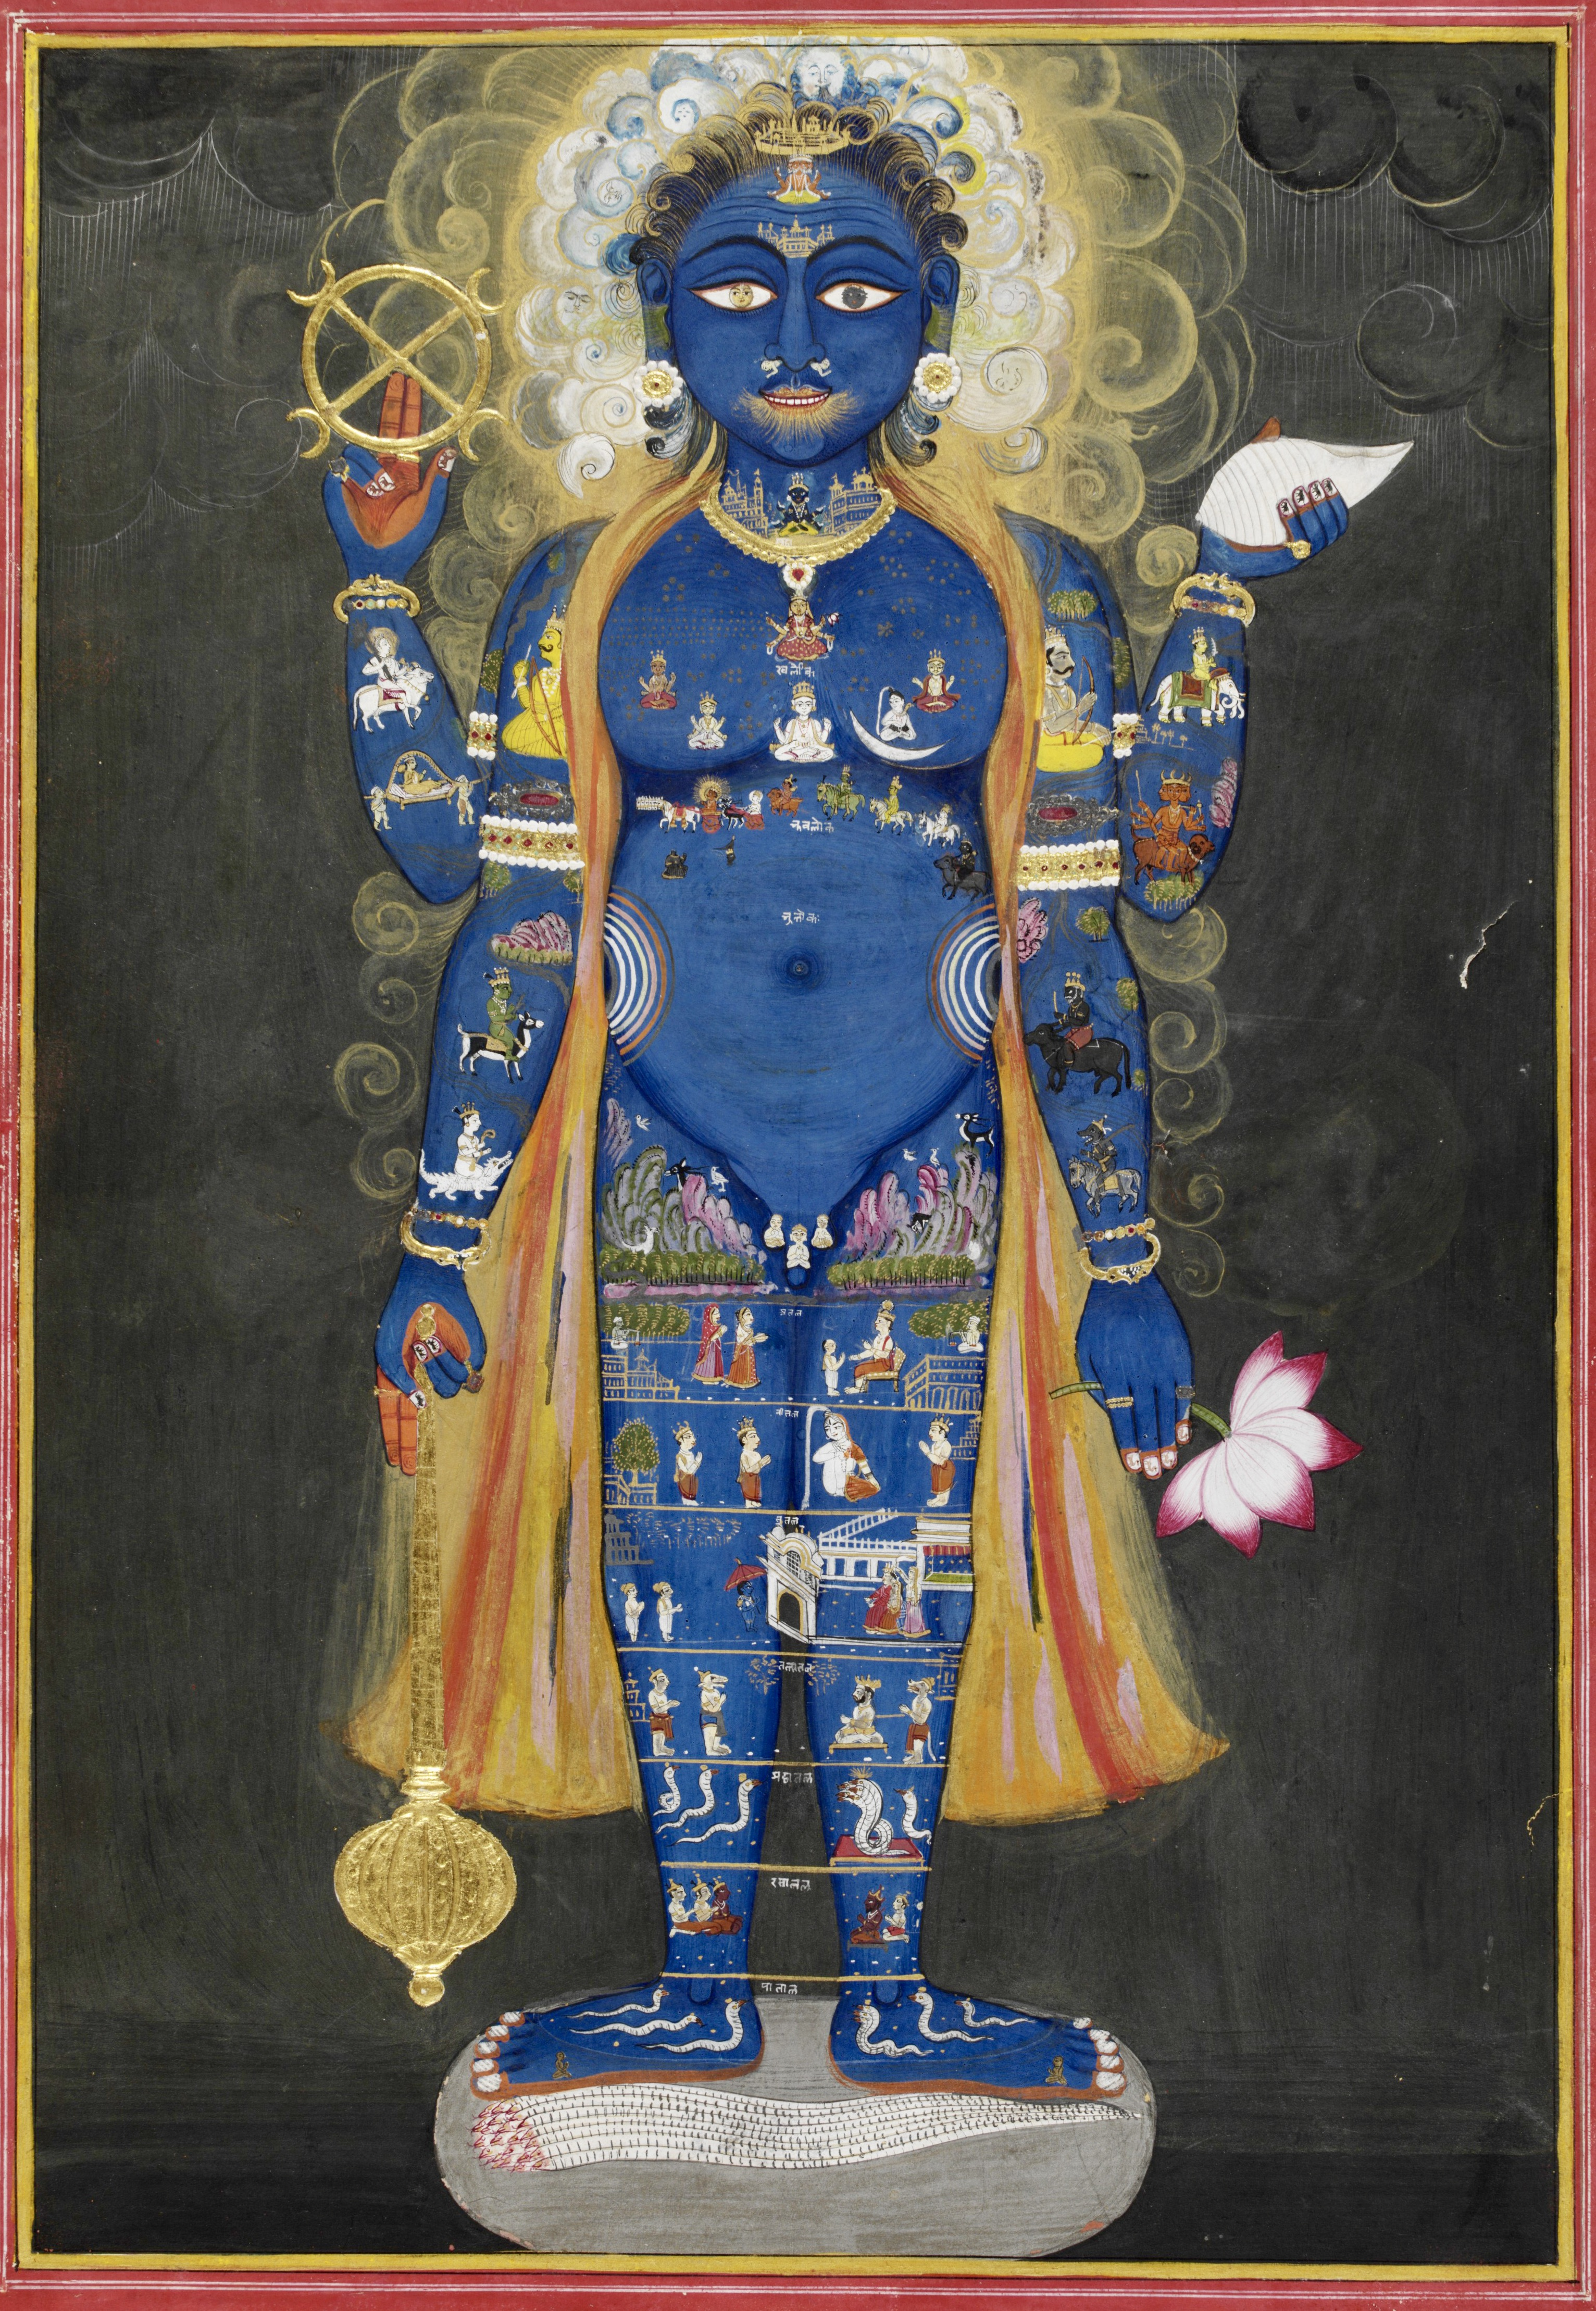
\includegraphics[width=1\textwidth]{pics/Vishnu_Vishvarupa_cropped.jpg}
	\caption{Viṣṇu Viśvarūpa, India, Rajasthan, Jaipur, ca. 1800–1820, Opaque watercolor and gold on paper, 38.5 × 28 cm, Victoria and Albert Museum, London, Given by Mrs. Gerald Clark.}
	\label{fig1}
      \end{figure}
\clearpage
  \begin{figure}[ht]
	\centering
  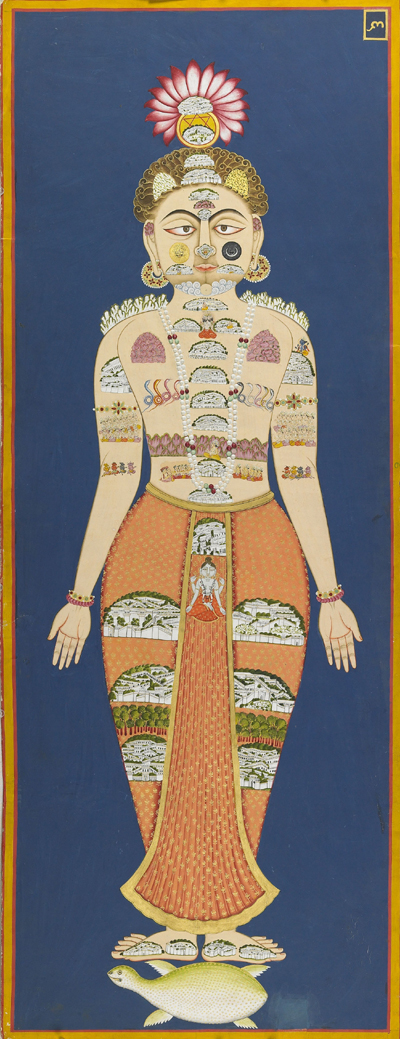
\includegraphics[width=0.5\textwidth]{pics/The_Equivalence_of_Self_and_Universe_(detail),_folio_6_from_the_Siddha_Siddhanta_Paddhati,_(Bulaki),_1824_(Samvat_1881);_122_x_46_cm._Mehrangarh_Museum_Trust..jpg}
	\caption{The Equivalence of Self and Universe (detail), folio 6 from the \textit{Siddhasiddhāntapaddhati} (Bulaki), India, Rajasthan, Jodhpur, 1824 (Samvat 1881), 122 x 46 cm, RJS 2378, Mehragarh Museum Trust.}
	\label{fig2}
      \end{figure}
      % \end{landscape}


\chapter{Bibliography}
 \label{sec:bibli}
   \clearpage
\newpage 
\thispagestyle{empty}
\quad  \addtocounter{page}{-1}

\printbibliography[heading=subbibintoc, title=Consulted Manuscripts, keyword=codex]

\printbibliography[heading=subbibintoc, title=Printed Editions, keyword=printsource]

\printbibliography[heading=subbibintoc, title=Secondary Literature, keyword=seclit]

\printbibliography[heading=subbibintoc, title=Online Sources, keyword=onlinesource]

\end{document}
